% Options for packages loaded elsewhere
\PassOptionsToPackage{unicode}{hyperref}
\PassOptionsToPackage{hyphens}{url}
%
\documentclass[
]{book}
\usepackage{amsmath,amssymb}
\usepackage{lmodern}
\usepackage{iftex}
\ifPDFTeX
  \usepackage[T1]{fontenc}
  \usepackage[utf8]{inputenc}
  \usepackage{textcomp} % provide euro and other symbols
\else % if luatex or xetex
  \usepackage{unicode-math}
  \defaultfontfeatures{Scale=MatchLowercase}
  \defaultfontfeatures[\rmfamily]{Ligatures=TeX,Scale=1}
\fi
% Use upquote if available, for straight quotes in verbatim environments
\IfFileExists{upquote.sty}{\usepackage{upquote}}{}
\IfFileExists{microtype.sty}{% use microtype if available
  \usepackage[]{microtype}
  \UseMicrotypeSet[protrusion]{basicmath} % disable protrusion for tt fonts
}{}
\makeatletter
\@ifundefined{KOMAClassName}{% if non-KOMA class
  \IfFileExists{parskip.sty}{%
    \usepackage{parskip}
  }{% else
    \setlength{\parindent}{0pt}
    \setlength{\parskip}{6pt plus 2pt minus 1pt}}
}{% if KOMA class
  \KOMAoptions{parskip=half}}
\makeatother
\usepackage{xcolor}
\IfFileExists{xurl.sty}{\usepackage{xurl}}{} % add URL line breaks if available
\IfFileExists{bookmark.sty}{\usepackage{bookmark}}{\usepackage{hyperref}}
\hypersetup{
  pdftitle={A Little Book of R for Bioinformatics 2.0},
  pdfauthor={Avirl Coghlan, with contributions by Nathan L. Brouwer},
  hidelinks,
  pdfcreator={LaTeX via pandoc}}
\urlstyle{same} % disable monospaced font for URLs
\usepackage{color}
\usepackage{fancyvrb}
\newcommand{\VerbBar}{|}
\newcommand{\VERB}{\Verb[commandchars=\\\{\}]}
\DefineVerbatimEnvironment{Highlighting}{Verbatim}{commandchars=\\\{\}}
% Add ',fontsize=\small' for more characters per line
\usepackage{framed}
\definecolor{shadecolor}{RGB}{248,248,248}
\newenvironment{Shaded}{\begin{snugshade}}{\end{snugshade}}
\newcommand{\AlertTok}[1]{\textcolor[rgb]{0.94,0.16,0.16}{#1}}
\newcommand{\AnnotationTok}[1]{\textcolor[rgb]{0.56,0.35,0.01}{\textbf{\textit{#1}}}}
\newcommand{\AttributeTok}[1]{\textcolor[rgb]{0.77,0.63,0.00}{#1}}
\newcommand{\BaseNTok}[1]{\textcolor[rgb]{0.00,0.00,0.81}{#1}}
\newcommand{\BuiltInTok}[1]{#1}
\newcommand{\CharTok}[1]{\textcolor[rgb]{0.31,0.60,0.02}{#1}}
\newcommand{\CommentTok}[1]{\textcolor[rgb]{0.56,0.35,0.01}{\textit{#1}}}
\newcommand{\CommentVarTok}[1]{\textcolor[rgb]{0.56,0.35,0.01}{\textbf{\textit{#1}}}}
\newcommand{\ConstantTok}[1]{\textcolor[rgb]{0.00,0.00,0.00}{#1}}
\newcommand{\ControlFlowTok}[1]{\textcolor[rgb]{0.13,0.29,0.53}{\textbf{#1}}}
\newcommand{\DataTypeTok}[1]{\textcolor[rgb]{0.13,0.29,0.53}{#1}}
\newcommand{\DecValTok}[1]{\textcolor[rgb]{0.00,0.00,0.81}{#1}}
\newcommand{\DocumentationTok}[1]{\textcolor[rgb]{0.56,0.35,0.01}{\textbf{\textit{#1}}}}
\newcommand{\ErrorTok}[1]{\textcolor[rgb]{0.64,0.00,0.00}{\textbf{#1}}}
\newcommand{\ExtensionTok}[1]{#1}
\newcommand{\FloatTok}[1]{\textcolor[rgb]{0.00,0.00,0.81}{#1}}
\newcommand{\FunctionTok}[1]{\textcolor[rgb]{0.00,0.00,0.00}{#1}}
\newcommand{\ImportTok}[1]{#1}
\newcommand{\InformationTok}[1]{\textcolor[rgb]{0.56,0.35,0.01}{\textbf{\textit{#1}}}}
\newcommand{\KeywordTok}[1]{\textcolor[rgb]{0.13,0.29,0.53}{\textbf{#1}}}
\newcommand{\NormalTok}[1]{#1}
\newcommand{\OperatorTok}[1]{\textcolor[rgb]{0.81,0.36,0.00}{\textbf{#1}}}
\newcommand{\OtherTok}[1]{\textcolor[rgb]{0.56,0.35,0.01}{#1}}
\newcommand{\PreprocessorTok}[1]{\textcolor[rgb]{0.56,0.35,0.01}{\textit{#1}}}
\newcommand{\RegionMarkerTok}[1]{#1}
\newcommand{\SpecialCharTok}[1]{\textcolor[rgb]{0.00,0.00,0.00}{#1}}
\newcommand{\SpecialStringTok}[1]{\textcolor[rgb]{0.31,0.60,0.02}{#1}}
\newcommand{\StringTok}[1]{\textcolor[rgb]{0.31,0.60,0.02}{#1}}
\newcommand{\VariableTok}[1]{\textcolor[rgb]{0.00,0.00,0.00}{#1}}
\newcommand{\VerbatimStringTok}[1]{\textcolor[rgb]{0.31,0.60,0.02}{#1}}
\newcommand{\WarningTok}[1]{\textcolor[rgb]{0.56,0.35,0.01}{\textbf{\textit{#1}}}}
\usepackage{longtable,booktabs,array}
\usepackage{calc} % for calculating minipage widths
% Correct order of tables after \paragraph or \subparagraph
\usepackage{etoolbox}
\makeatletter
\patchcmd\longtable{\par}{\if@noskipsec\mbox{}\fi\par}{}{}
\makeatother
% Allow footnotes in longtable head/foot
\IfFileExists{footnotehyper.sty}{\usepackage{footnotehyper}}{\usepackage{footnote}}
\makesavenoteenv{longtable}
\usepackage{graphicx}
\makeatletter
\def\maxwidth{\ifdim\Gin@nat@width>\linewidth\linewidth\else\Gin@nat@width\fi}
\def\maxheight{\ifdim\Gin@nat@height>\textheight\textheight\else\Gin@nat@height\fi}
\makeatother
% Scale images if necessary, so that they will not overflow the page
% margins by default, and it is still possible to overwrite the defaults
% using explicit options in \includegraphics[width, height, ...]{}
\setkeys{Gin}{width=\maxwidth,height=\maxheight,keepaspectratio}
% Set default figure placement to htbp
\makeatletter
\def\fps@figure{htbp}
\makeatother
\setlength{\emergencystretch}{3em} % prevent overfull lines
\providecommand{\tightlist}{%
  \setlength{\itemsep}{0pt}\setlength{\parskip}{0pt}}
\setcounter{secnumdepth}{5}
\usepackage{booktabs}

\usepackage{fontspec}
\usepackage{multirow}
\usepackage{multicol}
\usepackage{colortbl}
\usepackage{hhline}
\usepackage{longtable}
\usepackage{array}
\usepackage{hyperref}
\ifLuaTeX
  \usepackage{selnolig}  % disable illegal ligatures
\fi
\usepackage[]{natbib}
\bibliographystyle{apalike}

\title{A Little Book of R for Bioinformatics 2.0}
\author{Avirl Coghlan, with contributions by Nathan L. Brouwer}
\date{2021-08-09}

\begin{document}
\maketitle

{
\setcounter{tocdepth}{1}
\tableofcontents
}
\hypertarget{preface-to-version-2.0}{%
\chapter*{Preface to version 2.0}\label{preface-to-version-2.0}}
\addcontentsline{toc}{chapter}{Preface to version 2.0}

Welcome to \emph{A Little Book of R for Bioinformatics 2.0}!.

This book is based on the original \href{https://a-little-book-of-r-for-bioinformatics.readthedocs.io/en/latest/}{\emph{A Little Book of R for Bioinformatics}} by Dr.~Avril Coghlan (Hereafter ``ALBRB 1.0''). Dr.~Coghlan's book was one of the first and most thorough introductions to using \emph{R} for bioinformatics and computational biology, and was generously published under the Creative Commons 3.0 Attribution License \href{https://creativecommons.org/licenses/by/3.0/}{(CC BY 3.0)}. In addition to describing how to do bioinformatics in R, Coghlan provided numerous functions to facilitate important tasks, practice questions, and references to further reading.

\href{https://a-little-book-of-r-for-bioinformatics.readthedocs.io/en/latest/}{ALBRB 1.0} was extremely useful to me when I was learning bioinformatics and computational biology. In this version of the book, which I'll refer to as \textbf{ALBRB 2.0}, I have adapted Dr.~Coghlan's original book to suit my own teaching needs, updated it with current packages now available in R, added background materials from other open-access sources, and added in my original materials.

Below I've outlined the general types of changes I've made to the original book. I have tried to link back to the original content that these updates are derived from and note how changes were made. Any errors or inconsistencies should be ascribed to me, not Dr.~Coghlan. If you have any feedback, please email me at \href{mailto:brouwern@gmail.com}{\nolinkurl{brouwern@gmail.com}}

\textasciitilde Nathan Brouwer, June 2021

\textbf{Changes implemented in ALBRB 2.0 by Nathan Brouwer}

\begin{enumerate}
\def\labelenumi{\arabic{enumi}.}
\tightlist
\item
  Converted the entire book to RMarkdown and published it via \texttt{bookdown}.
\item
  Added instructions for using RStudio and RStudio Cloud.
\item
  Updated instructions to reflect any changes in software, including changes to how the bioinformatics repository \texttt{Bioconductor} now works.
\item
  Split up chapters into smaller units.
\item
  Reorganized the order of some material.
\item
  Added biological background information by integrating information from the Open Access textbook \href{https://bio.libretexts.org/Bookshelves/Introductory_and_General_Biology/Book\%3A_General_Biology_(OpenStax)}{LibreText General Biology}
\item
  Added links to the books I am developing, \emph{Get R Done!} and \emph{Computational Biology for All}.
\item
  Moved functions written by Coghlan and datasets to my teaching package \href{https://github.com/brouwern/compbio4all}{compbio4all}.
\item
  Functions names changed from camelCase to snake\_case
\item
  Functions re-written so as not to use Bioconductor to reduce/eliminate dependency of \texttt{compbio4all} on \texttt{Bioconductor}.
\item
  Changed some plotting to ggplot2 or ggpubr.
\item
  Added additional subheadings
\item
  Added vocab and function lists to the beginning of many chapters
\item
  At times replaced non-biological examples with biological ones.
\item
  Change from British to American English (Sorry! Couldn't help myself - the spellchecker made me do it!)
\item
  Provided additional links to external resources.
\item
  Added use of \texttt{rentrez} for querying NCBI databases
\end{enumerate}

\hypertarget{how-to-review-this-book}{%
\chapter{How to review this book}\label{how-to-review-this-book}}

\hypertarget{file-format}{%
\section{File format}\label{file-format}}

These lessons are written in RStudio using RMarkdown. Each .RMd file is a mix of test, written in plain format, and \textbf{code chunks}, which look like this

Code chunks start with there apostrophes and \{r\}, like this: ```\{r\}. They end with three apostrophes```. They will appear gray when opened up in RStudio but be white in the normal R code editor or other text editor.

\hypertarget{what-can-you-do}{%
\section{What can you do?}\label{what-can-you-do}}

\begin{itemize}
\tightlist
\item
  Read and fix typos : )
\item
  Add comments within the file
\item
  Email me general comments about the files (structure, topics, confusing parts etc)
\end{itemize}

\hypertarget{adding-comments}{%
\section{Adding comments}\label{adding-comments}}

You're welcome to add comments anywhere to the files, do the exercises and type up the key, propose you own exercises, etc.

\hypertarget{html-tagged-comments}{%
\subsection{HTML-tagged comments}\label{html-tagged-comments}}

The easiest way is to type a comment into the normal text part of the .Rmd file and then surround it with an html comment tag. A comment saying ``A comment'' will therefore look like this:

In RStudio you can type up a comment, highlight it then hit Shift+Control+C on a PC or Shift+Command+C on a mac.

\hypertarget{code-chunk-comments}{%
\subsection{Code chunk comments}\label{code-chunk-comments}}

Another way to add a comment is to make a RMarkdown code chunk thne type up your comments in it by commenting out each line, like the one below. Key to doing this is to put eval = F, echo = F in the braces after the r. eval = F, echo = F tells RStudio to leave that alone when the .Rmd file gets rendered into and web page or PDF.

In RStudio you can add code chunks with a shortcut key. On a Mac the shortcut is OPTION + COMMAND + I.

\hypertarget{keys-to-exercise}{%
\subsection{Keys to exercise}\label{keys-to-exercise}}

Some files will have exercises at the end. I don't always include the key, and you're welcome to try the exercise and type up a key (or fix any errors in mine). As for code chunk comments include eval = F, echo = F in the braces so the key won't appear when rendered. So a problem and its key would look something like this

\hypertarget{problem---fix-this-code}{%
\subsection{Problem - fix this code}\label{problem---fix-this-code}}

\begin{Shaded}
\begin{Highlighting}[]
\FunctionTok{print}\NormalTok{(correct answer)}
\end{Highlighting}
\end{Shaded}

\hypertarget{test-audio-link}{%
\chapter{Test audio link}\label{test-audio-link}}

Here is an example of an audio link embedded in a bookdown book.

The link is here:
\url{https://www.genome.gov/sites/default/files/tg/en/narration/single_nucleotide_polymorphisms_snps.mp3}

In HTML bookdown renders it like this:

(In PDF there is a way to render just a screen shot and link, I think).

\hypertarget{test-shiny-app}{%
\chapter{Test shiny app}\label{test-shiny-app}}

Here is an example of a Shiny app (treesiftr) embedded in a bookdown book.

The direct link is \href{https://wrightaprilm.shinyapps.io/treesiftr_app/}{here}:
\url{https://wrightaprilm.shinyapps.io/treesiftr_app/}

It may take a few seconds for the app to appear (its a fairly big one I think)

\hypertarget{test-youtube-vidoe}{%
\chapter{Test YouTube vidoe}\label{test-youtube-vidoe}}

Here is an example of a YouTube video embedded in a bookdown book.

\textbf{THIS FUNCTIONALITY CURRENTLY ISN''T WORKING BUT WAS PREVIOUSLY}

The \href{https://www.youtube.com/watch?v=zNzZ1PfUDNk\&feature=youtu.be}{original link} is: \url{https://www.youtube.com/watch?v=zNzZ1PfUDNk\&feature=youtu.be}

\hypertarget{test-google-doc-insertion}{%
\chapter{Test google doc insertion}\label{test-google-doc-insertion}}

A Google spreadsheet (or other google docs / form) can be embedded.

The original link is:
\url{https://docs.google.com/spreadsheets/d/18dt7cYHAaszV5Iq8Y-7YOEFnv6hIXbD39Vn75-c3fQo/edit?usp=sharing}

\begin{Shaded}
\begin{Highlighting}[]
\NormalTok{knitr}\SpecialCharTok{::}\FunctionTok{include\_url}\NormalTok{(}\AttributeTok{url =}\StringTok{"https://docs.google.com/spreadsheets/d/18dt7cYHAaszV5Iq8Y{-}7YOEFnv6hIXbD39Vn75{-}c3fQo/edit?usp=sharing"}\NormalTok{)}
\end{Highlighting}
\end{Shaded}

\href{https://docs.google.com/spreadsheets/d/18dt7cYHAaszV5Iq8Y-7YOEFnv6hIXbD39Vn75-c3fQo/edit?usp=sharing}{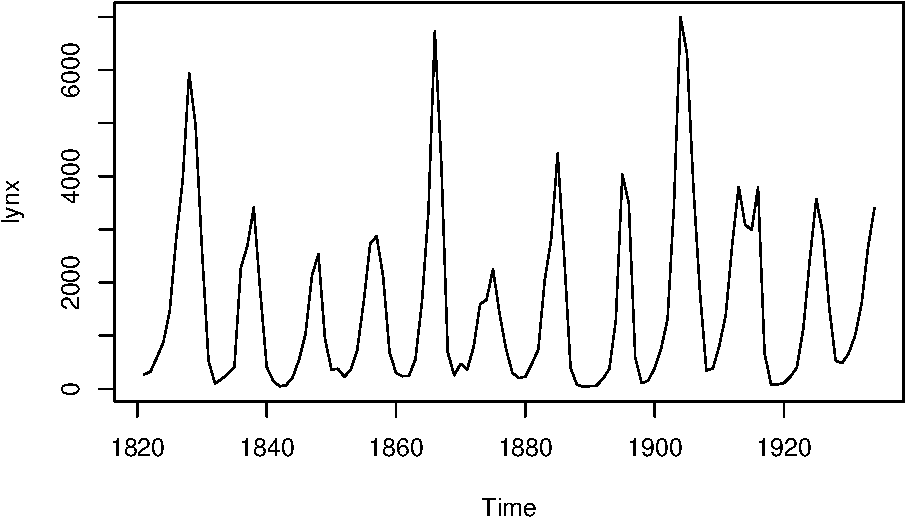
\includegraphics{lbrb_files/figure-latex/unnamed-chunk-9-1.pdf}}

\hypertarget{datacamp-test}{%
\chapter{Datacamp test}\label{datacamp-test}}

This an example of an embedded Datacamp tutorial. It will only be rendered in HTML output.

By default, \texttt{tutorial} will convert all R chunks.

\begin{Shaded}
\begin{Highlighting}[]
\NormalTok{a }\OtherTok{\textless{}{-}} \DecValTok{2}
\NormalTok{b }\OtherTok{\textless{}{-}} \DecValTok{3}

\NormalTok{a }\SpecialCharTok{+}\NormalTok{ b}
\end{Highlighting}
\end{Shaded}

\hypertarget{an-example-of-a-plotly-graph}{%
\chapter{An example of a plotly graph}\label{an-example-of-a-plotly-graph}}

The normal version of the graph looks like this.
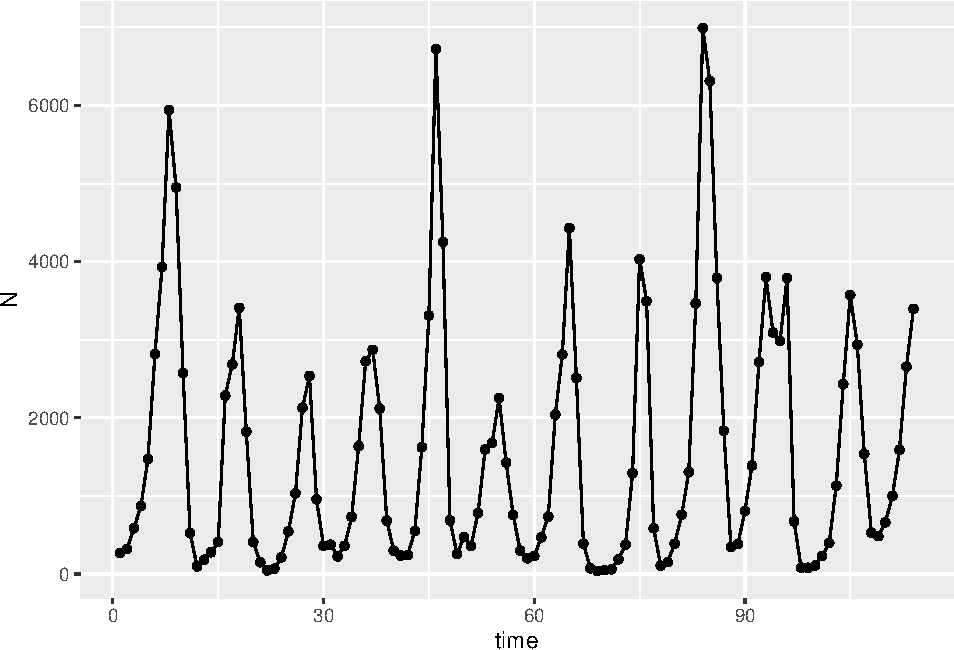
\includegraphics{lbrb_files/figure-latex/unnamed-chunk-12-1.pdf}

The plotly version looks like this

\begin{Shaded}
\begin{Highlighting}[]
\NormalTok{fig }\OtherTok{\textless{}{-}}\NormalTok{ plotly}\SpecialCharTok{::}\FunctionTok{ggplotly}\NormalTok{(p)}

\NormalTok{fig}
\end{Highlighting}
\end{Shaded}

\hypertarget{directly-embedding-of-a-libretext-page}{%
\chapter{Directly embedding of a libretext page}\label{directly-embedding-of-a-libretext-page}}

This is a libretext page directly called from bookdown and embedded in HTML

\hypertarget{libretext-image}{%
\chapter{Libretext image}\label{libretext-image}}

I've mocked up the content from a libretext page below. The main goal is to show how the image from this page doesn't need to be saved as a file, but can be pulled from librtext.

The original page is:

\url{https://bio.libretexts.org/Bookshelves/Introductory_and_General_Biology/Book\%3A_General_Biology_(OpenStax)/8\%3A_Ecology/45\%3A_Population_and_Community_Ecology/45.0\%3A_Prelude_to_Population_and_Community_Ecology}

\hypertarget{prelude-to-population-and-community-ecology}{%
\section{45.0: Prelude to Population and Community Ecology}\label{prelude-to-population-and-community-ecology}}

Imagine sailing down a river in a small motorboat on a weekend afternoon; the water is smooth and you are enjoying the warm sunshine and cool breeze when suddenly you are hit in the head by a 20-pound silver carp. This is a risk now on many rivers and canal systems in Illinois and Missouri because of the presence of Asian carp.

\begin{figure}
\href{https://bio.libretexts.org/@api/deki/files/2180/Figure_45_00_01.jpg?revision=1}{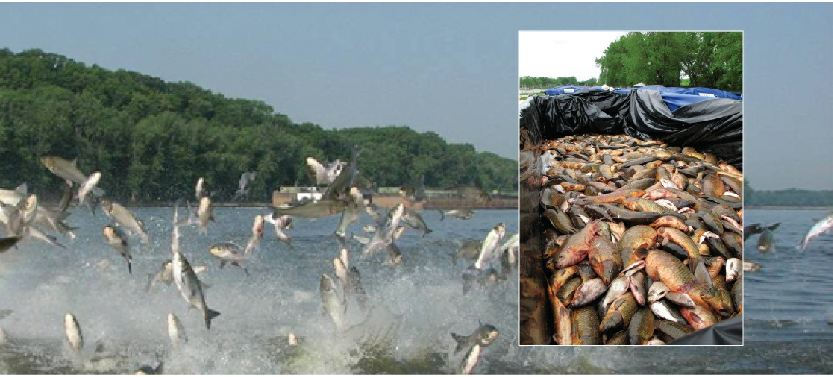
\includegraphics[width=0.5\linewidth]{lbrb_files/figure-latex/unnamed-chunk-15-1} }\caption{Figure  45.0.1 : Asian carp jump out of the water in response to electrofishing. The Asian carp in the inset photograph were harvested from the Little Calumet River in Illinois in May, 2010, using rotenone, a toxin often used as an insecticide, in an effort to learn more about the population of the species. (credit main image: modification of work by USGS; credit inset: modification of work by Lt. David French, USCG)}\label{fig:unnamed-chunk-15}
\end{figure}

This fish---actually a group of species including the silver, black, grass, and big head carp---has been farmed and eaten in China for over 1000 years. It is one of the most important aquaculture food resources worldwide. In the United States, however, Asian carp is considered a dangerous invasive species that disrupts community structure and composition to the point of threatening native species.

\hypertarget{note}{%
\section{Note}\label{note}}

the code to put the image in is

\begin{Shaded}
\begin{Highlighting}[]
\NormalTok{knitr}\SpecialCharTok{::}\FunctionTok{include\_url}\NormalTok{(}\StringTok{"https://bio.libretexts.org/@api/deki/files/2180/Figure\_45\_00\_01.jpg?revision=1"}\NormalTok{)}
\end{Highlighting}
\end{Shaded}

\hypertarget{nucleic-acids}{%
\chapter{Nucleic Acids}\label{nucleic-acids}}

\textbf{Authors}: OpenStax / Libretext Formatted in RMarkdown by Nathan Brouwer under the Creative Commons Attribution License 4.0 license.

This chapter was adapted from \href{https://bio.libretexts.org/Bookshelves/Introductory_and_General_Biology/Book\%3A_General_Biology_(OpenStax)}{LibreText General Biology}, Chapter 3, Section 3.5: \href{https://bio.libretexts.org/Bookshelves/Introductory_and_General_Biology/Book\%3A_General_Biology_(OpenStax)/1\%3A_The_Chemistry_of_Life/3\%3A_Biological_Macromolecules/3.5\%3A_Nucleic_Acids}{Nucleic Acids}. The LibreText book is based on \href{https://openstax.org/details/books/biology-2e}{OpenStax Biology 2nd edition}, Chapter 3, Section 3.5: \href{https://openstax.org/books/biology-2e/pages/3-5-nucleic-acids}{Nucleic Acids}. A full list of authors is found under the \textbf{Contributors and Attributions} section at the end of this document.

\begin{quote}
Nucleic acids are the most important macromolecules for the continuity
of life. They carry the genetic blueprint of a cell and carry
instructions for the functioning of the cell.
\end{quote}

\hypertarget{dna-and-rna}{%
\section{DNA and RNA}\label{dna-and-rna}}

The two main types of nucleic acids are deoxyribonucleic acid (DNA)
and ribonucleic acid (RNA). DNA is the genetic material found in all
living organisms, ranging from single-celled bacteria to multicellular
mammals. It is found in the nucleus of eukaryotes and in the
organelles, chloroplasts, and mitochondria. In prokaryotes, the DNA is
not enclosed in a membranous envelope.

The entire genetic content of a cell is known as its genome, and the
study of genomes is genomics. In eukaryotic cells but not in
prokaryotes, DNA forms a complex with histone proteins to form
chromatin, the substance of eukaryotic chromosomes. A chromosome may
contain tens of thousands of genes. Many genes contain the information
to make protein products; other genes code for RNA products. DNA
controls all of the cellular activities by turning the genes ``on'' or
``off.''

The other type of nucleic acid, RNA, is mostly involved in protein
synthesis. The DNA molecules never leave the nucleus but instead use
an intermediary to communicate with the rest of the cell. This
intermediary is the messenger RNA (mRNA). Other types of RNA---like
rRNA, tRNA, and microRNA---are involved in protein synthesis and its
regulation.

DNA and RNA are made up of monomers known as nucleotides. The
nucleotides combine with each other to form a polynucleotide, DNA or
RNA. Each nucleotide is made up of three components: a nitrogenous
base, a pentose (five-carbon) sugar, and a phosphate group (Figure
3.5.1). Each nitrogenous base in a nucleotide is attached to a sugar
molecule, which is attached to one or more phosphate groups.

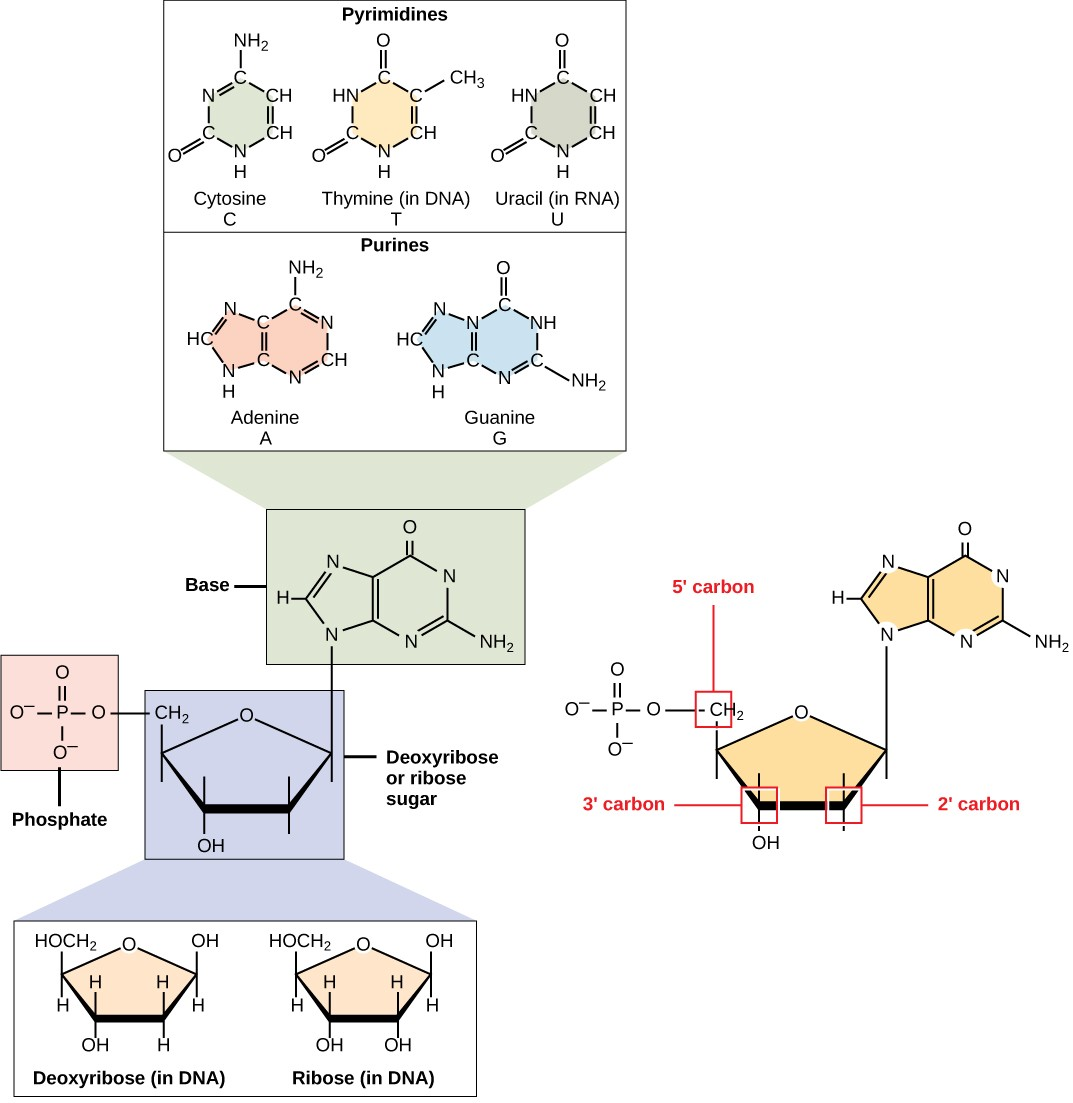
\includegraphics[width=14.9in]{/Users/nlb24/google_backup_sync_nlb24/lbrb/./images/image5}

Figure 3.5.1 : A nucleotide is made up of three components: a
nitrogenous base, a pentose sugar, and one or more phosphate groups.
Carbon residues in the pentose are numbered 1′ through 5′ (the prime
distinguishes these residues from those in the base, which are
numbered without using a prime notation). The base is attached to the
1′ position of the ribose, and the phosphate is attached to the 5′
position. When a polynucleotide is formed, the 5′ phosphate of the
incoming nucleotide attaches to the 3′ hydroxyl group at the end of
the growing chain. Two types of pentose are found in nucleotides,
deoxyribose (found in DNA) and ribose (found in RNA). Deoxyribose is
similar in structure to ribose, but it has an H instead of an OH at
the 2′ position. Bases can be divided into two categories: purines and
pyrimidines. Purines have a double ring structure, and pyrimidines
have a single ring.

The nitrogenous bases, important components of nucleotides, are
organic molecules and are so named because they contain carbon and
nitrogen. They are bases because they contain an amino group that has
the potential of binding an extra hydrogen, and thus, decreases the
hydrogen ion concentration in its environment, making it more basic.
Each nucleotide in DNA contains one of four possible nitrogenous
bases: adenine (A), guanine (G) cytosine (C), and thymine (T).

Adenine and guanine are classified as purines. The primary structure
of a purine is two carbon-nitrogen rings. Cytosine, thymine, and
uracil are classified as pyrimidines which have a single
carbon-nitrogen ring as their primary structure (Figure 3.5.1). Each
of these basic carbon-nitrogen rings has different functional groups
attached to it. In molecular biology shorthand, the nitrogenous bases are simply known by their symbols A, T, G, C, and U. DNA contains A, T, G, and C whereas RNA contains A, U, G, and
C.

The pentose sugar in DNA is deoxyribose, and in RNA, the sugar is
ribose (Figure 3.5.1). The difference between the sugars is the
presence of the hydroxyl group on the second carbon of the ribose and
hydrogen on the second carbon of the deoxyribose. The carbon atoms of
the sugar molecule are numbered as 1′, 2′, 3′, 4′, and 5′ (1′ is read
as ``one prime''). The phosphate residue is attached to the hydroxyl
group of the 5′ carbon of one sugar and the hydroxyl group of the 3′
carbon of the sugar of the next nucleotide, which forms a 5′--3′
phosphodiester linkage. The phosphodiester linkage is not formed by
simple dehydration reaction like the other linkages connecting
monomers in macromolecules: its formation involves the removal of two
phosphate groups. A polynucleotide may have thousands of such
phosphodiester linkages.

\hypertarget{dna-double-helix-structure}{%
\section{DNA Double-Helix Structure}\label{dna-double-helix-structure}}

DNA has a double-helix structure (Figure 3.5.2). The sugar and
phosphate lie on the outside of the helix, forming the backbone of the
DNA. The nitrogenous bases are stacked in the interior, like the steps
of a staircase, in pairs; the pairs are bound to each other by
hydrogen bonds. Every base pair in the double helivx is separated from
the next base pair by 0.34 nm. The two strands of the helix run in
opposite directions, meaning that the 5′ carbon end of one strand will
face the 3′ carbon end of its matching strand. (This is referred to as
antiparallel orientation and is important to DNA replication and in
many nucleic acid interactions.)

\begin{figure}
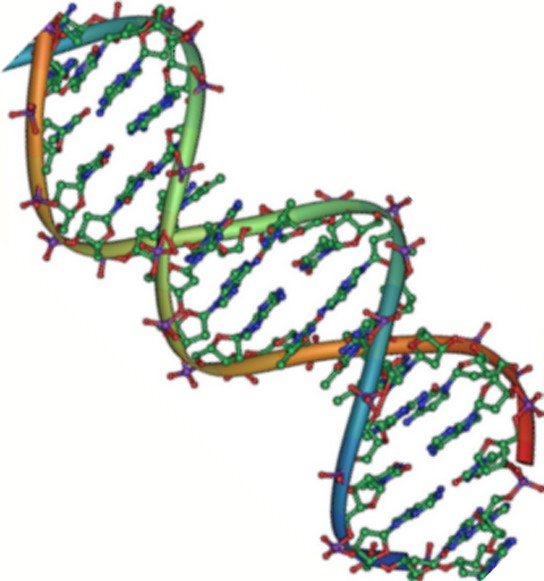
\includegraphics[width=7.56in]{/Users/nlb24/google_backup_sync_nlb24/lbrb/./images/image6} \caption{Figure 3.5.2 : Native DNA is an antiparallel double helix. The phosphate backbone (indicated by the curvy lines) is on the outside, and the bases are on the inside. Each base from one strand interacts via hydrogen bonding with a base from the opposing strand. (credit: Jerome Walker/Dennis Myts)}\label{fig:unnamed-chunk-18}
\end{figure}

Only certain types of base pairing are allowed. For example, a certain
purine can only pair with a certain pyrimidine. This means A can pair
with T, and G can pair with C, as shown in Figure 3.5.3. This is known
as the base complementary rule. In other words, the DNA strands are
complementary to each other. If the sequence of one strand is
AATTGGCC, the complementary strand would have the sequence TTAACCGG.
During DNA replication, each strand is copied, resulting in a daughter
DNA double helix containing one parental DNA strand and a newly
synthesized strand.

Art Connection

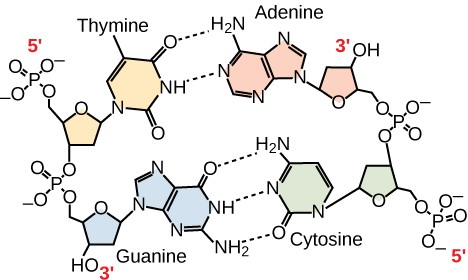
\includegraphics[width=6.5in]{/Users/nlb24/google_backup_sync_nlb24/lbrb/./images/image7}

Figure 3.5.3 : In a double stranded DNA molecule, the two strands run
antiparallel to one another so that one strand runs 5′ to 3′ and the
other 3′ to 5′. The phosphate backbone is located on the outside, and
the bases are in the middle. Adenine forms hydrogen bonds (or base
pairs) with thymine, and guanine base pairs with cytosine.

A mutation occurs, and cytosine is replaced with adenine. What impact
do you think this will have on the DNA structure?

\hypertarget{rna}{%
\section{RNA}\label{rna}}

Ribonucleic acid, or RNA, is mainly involved in the process of protein
synthesis under the direction of DNA. RNA is usually single-stranded
and is made of ribonucleotides that are linked by phosphodiester
bonds. A ribonucleotide in the RNA chain contains ribose (the pentose
sugar), one of the four nitrogenous bases (A, U, G, and C), and the
phosphate group.

There are four major types of RNA: messenger RNA (mRNA), ribosomal RNA
(rRNA), transfer RNA (tRNA), and microRNA (miRNA). The first, mRNA,
carries the message from DNA, which controls all of the cellular
activities in a cell. If a cell requires a certain protein to be
synthesized, the gene for this product is turned ``on'' and the
messenger RNA is synthesized in the nucleus. The RNA base sequence is
complementary to the coding sequence of the DNA from which it has been
copied. However, in RNA, the base T is absent and U is present
instead. If the DNA strand has a sequence AATTGCGC, the sequence of
the complementary RNA is UUAACGCG. In the cytoplasm, the mRNA
interacts with ribosomes and other cellular machinery (Figure 3.5.4).

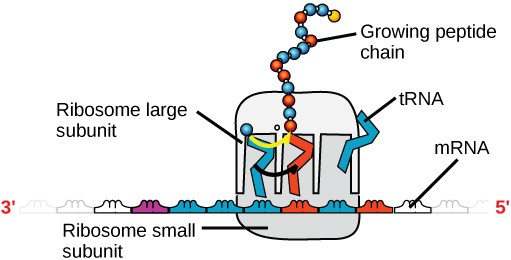
\includegraphics[width=7.1in]{/Users/nlb24/google_backup_sync_nlb24/lbrb/./images/image8}

Figure 3.5.4 : A ribosome has two parts: a large subunit and a small
subunit. The mRNA sits in between the two subunits. A tRNA molecule
recognizes a codon on the mRNA, binds to it by complementary base
pairing, and adds the correct amino acid to the growing peptide chain.

The mRNA is read in sets of three bases known as codons. Each codon
codes for a single amino acid. In this way, the mRNA is read and the
protein product is made. Ribosomal RNA (rRNA) is a major constituent
of ribosomes on which the mRNA binds. The rRNA ensures the proper
alignment of the mRNA and the ribosomes; the rRNA of the ribosome also
has an enzymatic activity (peptidyl transferase) and catalyzes the
formation of the peptide bonds between two aligned amino acids.
Transfer RNA (tRNA) is one of the smallest of the four types of RNA,
usually 70--90 nucleotides long. It carries the correct amino acid to
the site of protein synthesis. It is the base pairing between the tRNA
and mRNA that allows for the correct amino acid to be inserted in the
polypeptide chain. microRNAs are the smallest RNA molecules and their
role involves the regulation of gene expression by interfering with
the expression of certain mRNA messages. Table 3.5.1 below summarizes
features of DNA and RNA.

\textbf{\emph{Table}} 3.5.1 *\textbf{:} Features of DNA and RNA.

\begin{longtable}[]{@{}
  >{\raggedright\arraybackslash}p{(\columnwidth - 4\tabcolsep) * \real{0.31}}
  >{\raggedright\arraybackslash}p{(\columnwidth - 4\tabcolsep) * \real{0.35}}
  >{\raggedright\arraybackslash}p{(\columnwidth - 4\tabcolsep) * \real{0.35}}@{}}
\toprule
\begin{minipage}[b]{\linewidth}\raggedright
\end{minipage} & \begin{minipage}[b]{\linewidth}\raggedright
Features of DNA and
RNA
\end{minipage} & \begin{minipage}[b]{\linewidth}\raggedright
\end{minipage} \\
\midrule
\endhead
& DNA & RNA \\
Function & Carries genetic
information & Involved in protein
synthesis \\
Location & Remains in the nucleus & Leaves the nucleus \\
Structure & Double helix & Usually
single-stranded \\
Sugar & Deoxyribose & Ribose \\
Pyrimidines & Cytosine, thymine & Cytosine, uracil \\
Purines & Adenine, guanine & Adenine, guanine \\
\bottomrule
\end{longtable}

Even though the RNA is single stranded, most RNA types show extensive
intramolecular base pairing between complementary sequences, creating
a predictable three-dimensional structure essential for their
function.

As you have learned, information flow in an organism takes place from
DNA to RNA to protein. DNA dictates the structure of mRNA in a process
known as transcription, and RNA dictates the structure of protein in a
process known as translation. This is known as the Central Dogma of
Life, which holds true for all organisms; however, exceptions to the
rule occur in connection with viral infections.

\emph{Link to Learning}


\includegraphics[width=0.1\linewidth]{/Users/nlb24/google_backup_sync_nlb24/lbrb/./images/image9}

\begin{itemize}
\tightlist
\item
  To learn more about DNA, explore the Howard Hughes Medical Institute
  BioInteractive animations on the topic of DNA.*
\end{itemize}

\hypertarget{summary}{%
\section{Summary}\label{summary}}

Nucleic acids are molecules made up of nucleotides that direct
cellular activities such as cell division and protein synthesis. Each
nucleotide is made up of a pentose sugar, a nitrogenous base, and a
phosphate group. There are two types of nucleic acids: DNA and RNA.
DNA carries the genetic blueprint of the cell and is passed on from
parents to offspring (in the form of chromosomes). It has a
double-helical structure with the two strands running in opposite
directions, connected by hydrogen bonds, and complementary to each
other. RNA is single-stranded and is made of a pentose sugar (ribose),
a nitrogenous base, and a phosphate group. RNA is involved in protein
synthesis and its regulation. Messenger RNA (mRNA) is copied from the
DNA, is exported from the nucleus to the cytoplasm, and contains
information for the construction of proteins. Ribosomal RNA (rRNA) is
a part of the ribosomes at the site of protein synthesis, whereas
transfer RNA (tRNA) carries the amino acid to the site of protein
synthesis. microRNA regulates the use of mRNA for protein synthesis.

Art Connections

\hypertarget{analysis-questions}{%
\section{Analysis Questions}\label{analysis-questions}}

Free Response

\hypertarget{glossary}{%
\section{Glossary}\label{glossary}}

\textbf{deoxyribonucleic acid (DNA)}: double-helical molecule that carries the hereditary information of the cell\\
\textbf{messenger RNA (mRNA)}: DNA that carries information from DNA to ribosomes during proteinsynthesis\\
\textbf{nucleic acid}: biological macromolecule that carries the genetic blueprint of a cell
and carries instructions for the functioning of the cell\\
\textbf{nucleotide}: monomer of nucleic acids; contains a pentose sugar, one or more phosphate groups, and a nitrogenous base\\
\textbf{phosphodiester}: linkage covalent chemical bond that holds together the polynucleotide
chains with a phosphate group linking two pentose sugars of neighboring nucleotides\\
\textbf{polynucleotide}: long chain of nucleotides\\
\textbf{purine}: type of nitrogenous base in DNA and RNA; adenine and guanine are\\
\textbf{purines, pyrimidine}: type of nitrogenous base in DNA and RNA; cytosine, thymine, and uracil
are pyrimidines\\
\textbf{ribonucleic acid (RNA)}: single-stranded, often internally base paired, molecule that is
involved in protein synthesis\\
\textbf{ribosomal RNA (rRNA)}: RNA that ensures the proper alignment of the mRNA and the ribosomes
during protein synthesis and catalyzes the formation of the peptide linkage\\
\textbf{transcription}: process through which messenger RNA forms on a template of DNA\\
\textbf{transfer RNA (tRNA)}: RNA that carries activated amino acids to the site of protein
synthesis on the ribosome\\
\textbf{translation}: process through which RNA directs the formation of protein

\hypertarget{contributors-and-attributions}{%
\section{Contributors and Attributions}\label{contributors-and-attributions}}

Connie Rye (East Mississippi Community College), Robert Wise
(University of Wisconsin, Oshkosh), Vladimir Jurukovski (Suffolk
County Community College), Jean DeSaix (University of North Carolina
at Chapel Hill), Jung Choi (Georgia Institute of Technology), Yael
Avissar (Rhode Island College) among other contributing authors.
Original content by OpenStax (CC BY 4.0; Download for free at
\href{http://cnx.org/contents/185cbf87-c72e-48f5-b51e-f14f21b5eabd\%409.87}{http://cnx.org/contents/185cbf87-c72...f21b5eabd@9.87}).

\hypertarget{proteins}{%
\chapter{Proteins}\label{proteins}}

\textbf{Authors}: OpenStax / LibreText. Formatted in RMarkdown by Nathan Brouwer under the Creative Commons Attribution License 4.0 license.

This chapter was adapted from \href{}{LibreText General Biology}, Chapter 3, Section 3.4: \href{https://bio.libretexts.org/Bookshelves/Introductory_and_General_Biology/Book\%3A_General_Biology_(OpenStax)/1\%3A_The_Chemistry_of_Life/3\%3A_Biological_Macromolecules/3.4\%3A_Proteins}{Proteins}. The LibreText book is based on \href{https://openstax.org/details/books/biology-2e}{OpenStax Biology 2nd edition}, Chapter 3, Section 3.4: \href{https://openstax.org/books/biology-2e/pages/3-4-proteins}{Nucleic Acids}. A full list of authors is found under the \textbf{Contributors and Attributions} section at the end of this document.

\hypertarget{skills-to-develop}{%
\subsection{Skills to develop:}\label{skills-to-develop}}

\begin{enumerate}
\def\labelenumi{\arabic{enumi}.}
\tightlist
\item
  Describe the functions proteins perform in the cell and in tissues
\item
  Discuss the relationship between amino acids and proteins
\item
  Explain the four levels of protein organization
\item
  Describe the ways in which protein shape and function are linked
\end{enumerate}

Proteins are one of the most abundant organic molecules in living systems and have the most diverse range of functions of all \textbf{macromolecules}. Proteins may be structural, regulatory, contractile, or protective; they may serve in transport, storage, or membranes; or they may be toxins or enzymes. Each cell in a living system may contain thousands of proteins, each with a unique function. Their structures, like their functions, vary greatly. They are all, however, \textbf{polymers} of \textbf{amino acids}, arranged in a linear sequence.

\hypertarget{types-and-functions-of-proteins}{%
\section{Types and Functions of Proteins}\label{types-and-functions-of-proteins}}

\textbf{Enzymes}, which are produced by living cells, are \textbf{catalysts} in biochemical reactions (like digestion) and are usually complex or conjugated proteins. Each enzyme is specific for the substrate (a reactant that binds to an enzyme) it acts on. The enzyme may help in breakdown, rearrangement, or synthesis reactions. Enzymes that break down their substrates are called \textbf{catabolic enzymes}, enzymes that build more complex molecules from their substrates are called \textbf{anabolic enzymes}, and enzymes that affect the rate of reaction are called \textbf{catalytic enzymes}.
It should be noted that all enzymes increase the rate of reaction and, therefore, are considered to be organic catalysts. An example of an enzyme is salivary amylase, which
hydrolyzes its substrate amylose, a component of starch.

\textbf{Hormones} are chemical-signaling molecules, usually small proteins or steroids, secreted by endocrine cells that act to control or regulate specific physiological processes, including growth, development, metabolism, and reproduction. For example, insulin is a \textbf{protein hormone} that helps to regulate the blood glucose level.

Proteins have different shapes and molecular weights; some proteins are \textbf{globular} in shape whereas others are fibrous. For example, hemoglobin is a globular protein, but collagen, found in our skin, is a fibrous protein. Protein shape is critical to its function, and this shape is maintained by many different types of chemical bonds. Changes in temperature, pH, and exposure to chemicals may lead to permanent changes in the shape of the protein, leading to loss of function, known as \textbf{denaturation}. All proteins are made up of different arrangements of the same 20 types of \textbf{amino acids}.

\hypertarget{amino-acids}{%
\section{Amino Acids}\label{amino-acids}}

Amino acids are the \textbf{monomers} that make up proteins. Each amino acid has the same fundamental structure, which consists of a central carbon atom, also known as the alpha (\emph{α}) carbon, bonded to an amino group (NH\textsubscript{2}), a carboxyl group (COOH), and to a hydrogen atom. Every amino acid also has another atom or group of atoms bonded to the central atom known as the R group (Figure 3.4.1).

\begin{figure}
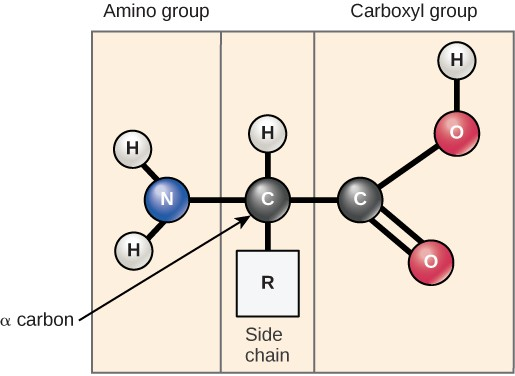
\includegraphics[width=7.15in]{/Users/nlb24/google_backup_sync_nlb24/lbrb/./images/protimage1} \caption{Amino acids have a central asymmetric carbon to which an amino group, a carboxyl group, a hydrogen atom, and a side chain (R group) are attached.}\label{fig:unnamed-chunk-22}
\end{figure}

The name ``amino acid'' is derived from the fact that they contain both an amino group and carboxyl-acid-group in their basic structure. For each amino acid, the R group (or side chain) is different (Figure 3.4.2).

\begin{figure}
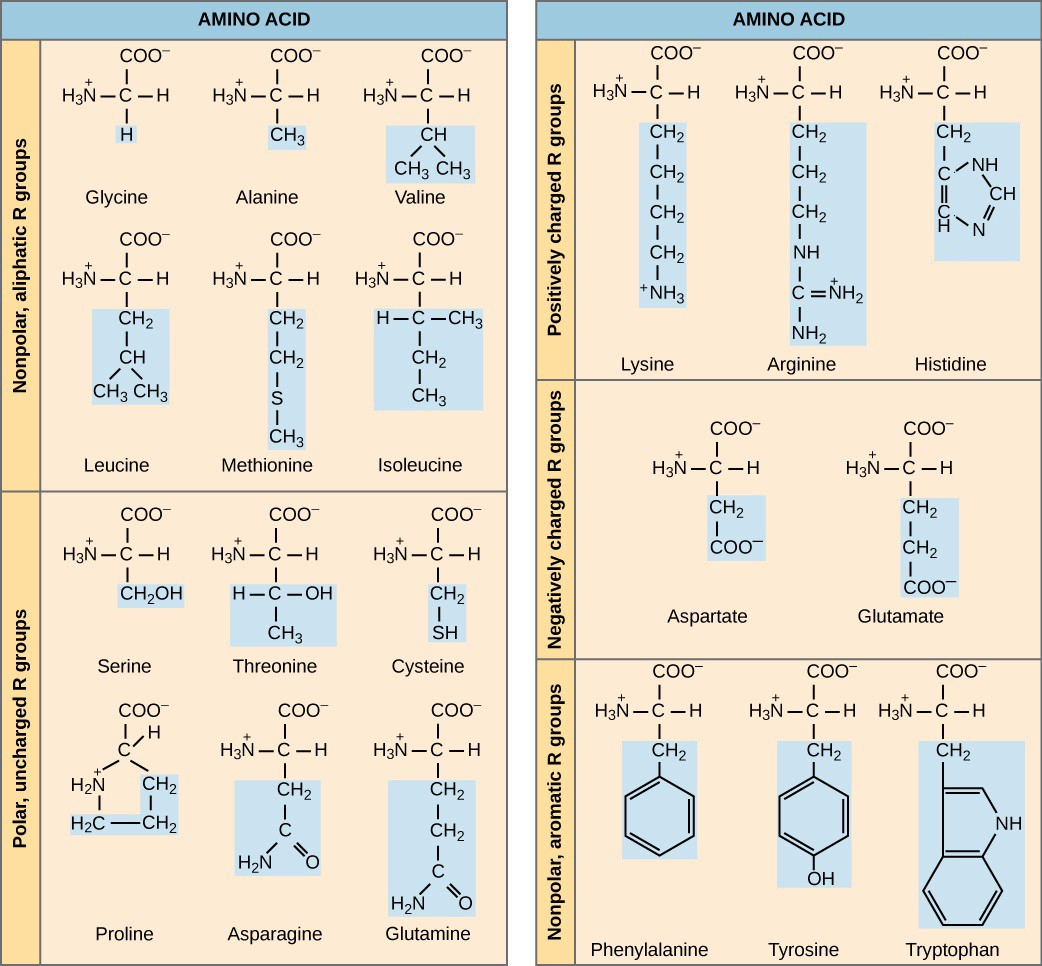
\includegraphics[width=14.47in]{/Users/nlb24/google_backup_sync_nlb24/lbrb/./images/protimage2} \caption{There are 20 common amino acids commonly found in proteins, each with a different R group (variant group) that determines its chemical nature.}\label{fig:unnamed-chunk-23}
\end{figure}

Which categories of amino acid would you expect to find on the surface
of a soluble protein, and which would you expect to find in the
interior? What distribution of amino acids would you expect to find in
a protein embedded in a lipid bilayer?

The chemical nature of the side chain determines the nature of the amino acid (that is, whether it is \textbf{acidic}, \textbf{basic}, \textbf{polar}, or \textbf{nonpolar}). For example, the amino acid glycine has a hydrogen atom as the R group. Amino acids such as valine, methionine, and alanine are nonpolar or hydrophobic, while amino acids such as serine, threonine, and cysteine are polar and have hydrophilic side chains. The side chains of lysine and arginine are positively charged, and therefore these amino acids are also known as basic amino acids. Proline has an R group that is linked to the amino group, forming a ring-like structure. Proline is an exception to the standard structure of an animo acid since its amino group is not separate from the side chain

Amino acids are represented by a single upper case letter or a three-letter abbreviation. For example, valine is known by the letter V or the three-letter code val.

The sequence and the number of amino acids ultimately determine a protein's shape, size, and function. Each amino acid is attached to another amino acid by a covalent bond, known as a \textbf{peptide bond}, which is formed by a dehydration reaction. The carboxyl group of one amino acid and the amino group of the incoming amino acid combine, releasing a molecule of water. The resulting bond is the peptide bond

\begin{figure}
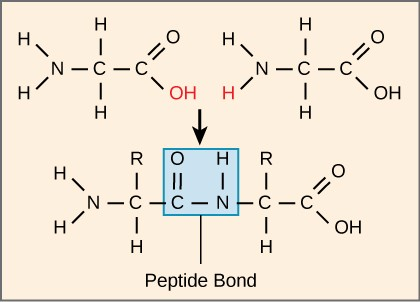
\includegraphics[width=5.83in]{/Users/nlb24/google_backup_sync_nlb24/lbrb/./images/protimage3} \caption{Peptide bond formation is a dehydration synthesis reaction. The carboxyl group of one amino acid is linked to the amino group of the incoming amino acid. In the process, a molecule of water is released.}\label{fig:unnamed-chunk-24}
\end{figure}

The products formed by such linkages are called \textbf{peptides}. As more amino acids join to this growing chain, the resulting chain is known as a \textbf{polypeptide}. Each polypeptide has a free amino group at one end. This end is called the \textbf{N-terminal}, or the amino terminal, and the other end has a free carboxyl group, also known as the C- or carboxyl
terminal. The terms polypeptide and protein are sometimes used interchangeably, a polypeptide is technically a polymer of amino acids, whereas the term protein is more formally used for a polypeptide or polypeptides that have combined together, often have bound non-peptide prosthetic groups, have a distinct shape, and have a unique function.

After \textbf{protein synthesis (translation)}, most proteins are modified. These are known as \textbf{post-translational modifications}. They may undergo \textbf{cleavage}, \textbf{phosphorylation} (addition of a phosphate group), or may require the addition of other chemical groups. Only after these modifications is the protein completely functional.

\hypertarget{evolution-connection}{%
\section{Evolution Connection:}\label{evolution-connection}}

\begin{longtable}[]{@{}
  >{\raggedright\arraybackslash}p{(\columnwidth - 0\tabcolsep) * \real{0.22}}@{}}
\toprule
\endhead
\textbf{The Evolutionary Significance of Cytochrome}: Cytochrome c is an
important component of the electron transport chain, a part of
cellular respiration, and it is normally found in the cellular
organelle, the mitochondrion. This protein has a heme prosthetic
group, and the central ion of the heme gets alternately reduced and
oxidized during electron transfer. Because this essential protein's
role in producing cellular energy is crucial, it has changed very
little over millions of years. Protein sequencing has shown that there
is a considerable amount of cytochrome c amino acid sequence \textbf{homology}
among different species; in other words, evolutionary kinship can be
assessed by measuring the similarities or differences among various
species' DNA or protein sequences. \\
Scientists have determined that human cytochrome c contains 104 amino
acids. For each cytochrome c molecule from different organisms that
has been sequenced to date, 37 of these amino acids appear in the same
position in all samples of cytochrome c.~This indicates that there may
have been a \textbf{common ancestor}. On comparing the human and chimpanzee
protein sequences, no sequence difference was found. When human and
rhesus monkey sequences were compared, the single difference found was
in one amino acid. In another comparison, human to yeast sequencing
shows a difference in the 44th position. \\
\bottomrule
\end{longtable}

\hypertarget{protein-structure}{%
\section{Protein Structure}\label{protein-structure}}

The shape of a protein is critical to its function. For example, an enzyme can bind to a specific substrate at a site known as the \textbf{active site}. If this active site is altered because of local changes or changes in overall protein structure, the enzyme may be unable to bind to the substrate. To understand how the protein gets its final shape or conformation, we need to understand the four levels of protein structure: primary, secondary, tertiary, and quaternary.

\hypertarget{primary-structure}{%
\subsection{Primary Structure}\label{primary-structure}}

The unique sequence of amino acids in a polypeptide chain is its
primary structure. For example, the pancreatic hormone insulin has two
polypeptide chains, A and B, and they are linked together by disulfide
bonds. The N terminal amino acid of the A chain is glycine, whereas
the C terminal amino acid is asparagine (Figure 3.4.4). The sequences
of amino acids in the A and B chains are unique to insulin.

\begin{figure}
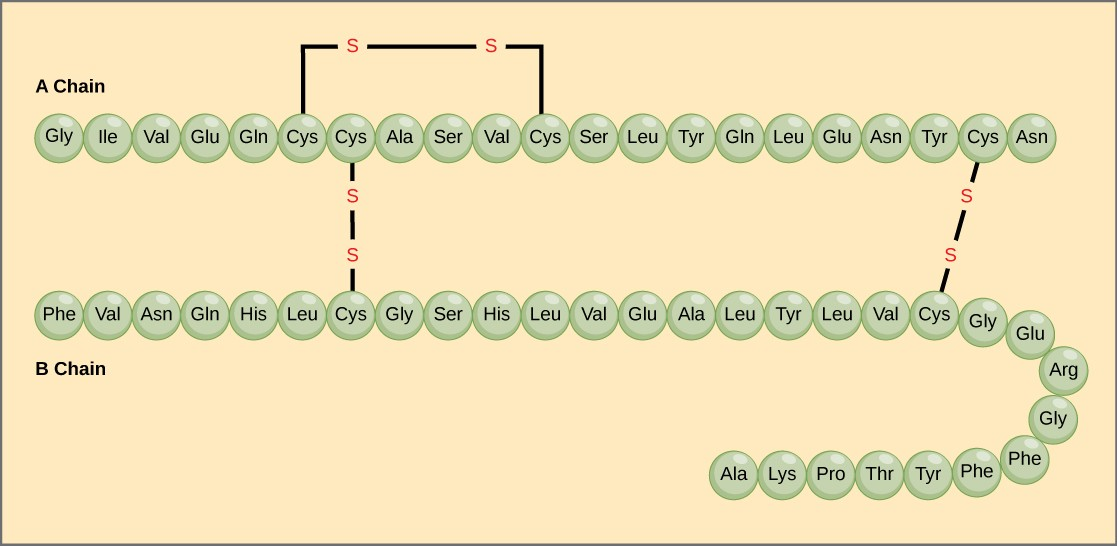
\includegraphics[width=15.51in]{/Users/nlb24/google_backup_sync_nlb24/lbrb/./images/protimage4} \caption{Bovine serum insulin is a protein hormone made of two peptide chains, A (21 amino acids long) and B (30 amino acids long). In each chain, primary structure is indicated by three-letter abbreviations that represent the names of the amino acids in the order they are present. The amino acid cysteine (cys) has a sulfhydryl (SH) group as a side chain. Two sulfhydryl groups can react in the presence of oxygen to form a disulfide (S-S) bond. Two disulfide bonds connect the A and B chains together, and a third helps the A chain fold into the correct shape. Note that all disulfide bonds are the same length, but are drawn different sizes for clarity.}\label{fig:unnamed-chunk-25}
\end{figure}

The unique sequence for every protein is ultimately determined by the
gene encoding the protein. A change in nucleotide sequence of the
gene's coding region may lead to a different amino acid being added to
the growing polypeptide chain, causing a change in protein structure
and function. In sickle cell anemia, the hemoglobin \emph{β} chain (a small
portion of which is shown in Figure 3.4.5) has a single amino acid
substitution, causing a change in protein structure and function.
Specifically, the amino acid glutamic acid is substituted by valine in
the beta chain. What is most remarkable to consider is that a
hemoglobin molecule is made up of two alpha chains and two beta chains
that each consist of about 150 amino acids. The molecule, therefore,
has about 600 amino acids. The structural difference between a normal
hemoglobin molecule and a sickle cell molecule---which dramatically
decreases life expectancy---is a single amino acid of the 600. What is
even more remarkable is that those 600 amino acids are encoded by
three nucleotides each, and the mutation is caused by a single base
change (point mutation), 1 in 1800 bases.

\begin{figure}
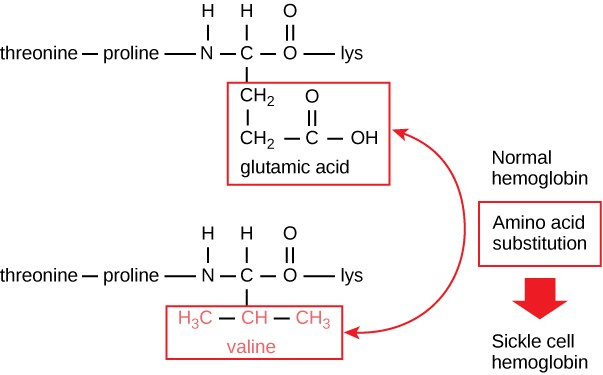
\includegraphics[width=8.38in]{/Users/nlb24/google_backup_sync_nlb24/lbrb/./images/protimage5} \caption{The beta chain of hemoglobin is 147 residues in length, yet a single amino acid substitution leads to sickle cell anemia. In normal hemoglobin, the amino acid at position seven is glutamate. In sickle cell hemoglobin, this glutamate is replaced by a valine.}\label{fig:unnamed-chunk-26}
\end{figure}

Because of this change of one amino acid in the chain, hemoglobin
molecules form long fibers that distort the biconcave, or disc-shaped,
red blood cells and assume a crescent or ``sickle'' shape, which clogs
arteries (Figure 3.4.6). This can lead to myriad serious health
problems such as breathlessness, dizziness, headaches, and abdominal
pain for those affected by this disease.

\begin{figure}
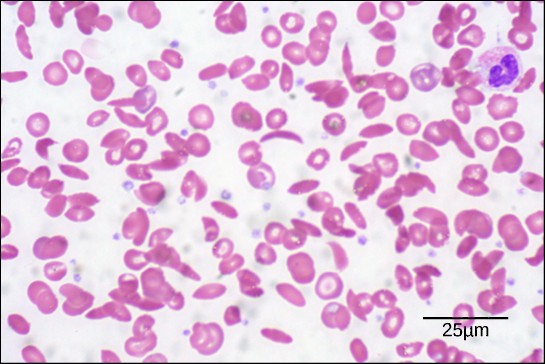
\includegraphics[width=7.57in]{/Users/nlb24/google_backup_sync_nlb24/lbrb/./images/protimage6} \caption{In this blood smear, visualized at 535x magnification using bright field microscopy, sickle cells are crescent shaped, while normal cells are disc-shaped. (credit: modification of work by Ed Uthman; scale-bar data from Matt Russell)}\label{fig:unnamed-chunk-27}
\end{figure}

\hypertarget{secondary-structure}{%
\subsection{Secondary Structure}\label{secondary-structure}}

The local folding of the polypeptide in some regions gives rise to the
secondary structure of the protein. The most common are the \emph{α}-helix
and \emph{β}-pleated sheet structures (Figure 3.4.7). Both structures are
the \emph{α}-helix structure---the helix held in shape by hydrogen bonds.
The hydrogen bonds form between the oxygen atom in the carbonyl group
in one amino acid and another amino acid that is four amino acids
farther along the chain.

\begin{figure}
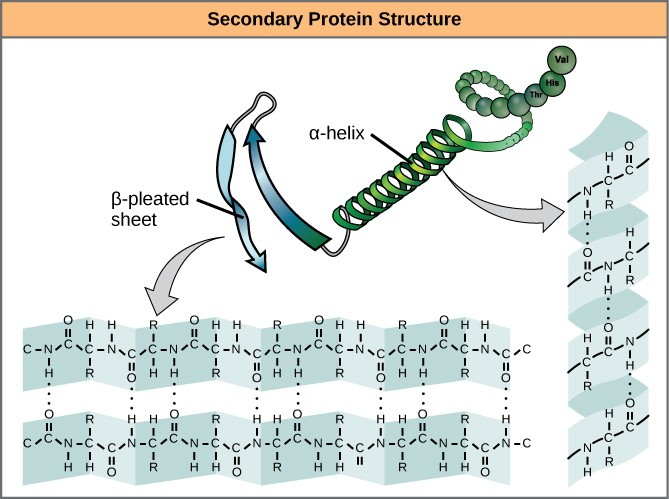
\includegraphics[width=9.29in]{/Users/nlb24/google_backup_sync_nlb24/lbrb/./images/protimage7} \caption{The α-helix and β-pleated sheet are secondary structures of proteins that form because of hydrogen bonding between carbonyl and amino groups in the peptide backbone. Certain amino acids have a propensity to form an α-helix, while others have a propensity to form a β-pleated sheet.}\label{fig:unnamed-chunk-28}
\end{figure}

Every helical turn in an alpha helix has 3.6 amino acid residues. The
R groups (the variant groups) of the polypeptide protrude out from the
\emph{α}-helix chain. In the \emph{β}-pleated sheet, the ``pleats'' are formed by
hydrogen bonding between atoms on the backbone of the polypeptide
chain. The R groups are attached to the carbons and extend above and
below the folds of the pleat. The pleated segments align parallel or
antiparallel to each other, and hydrogen bonds form between the
partially positive nitrogen atom in the amino group and the partially
negative oxygen atom in the carbonyl group of the peptide backbone.
The \emph{α}-helix and \emph{β}-pleated sheet structures are found in most
globular and fibrous proteins and they play an important structural
role.

\hypertarget{tertiary-structure}{%
\subsection{Tertiary Structure}\label{tertiary-structure}}

The unique three-dimensional structure of a polypeptide is its
tertiary structure (Figure 3.4.8). This structure is in part due to
chemical interactions at work on the polypeptide chain. Primarily, the
interactions among R groups creates the complex three- dimensional
tertiary structure of a protein. The nature of the R groups found in
the amino acids involved can counteract the formation of the hydrogen
bonds described for standard secondary structures. For example, R
groups with like charges are repelled by each other and those with
unlike charges are attracted to each other (ionic bonds). When protein
folding takes place, the hydrophobic R groups of nonpolar amino acids
lay in the interior of the protein, whereas the hydrophilic R groups
lay on the outside. The former types of interactions are also known as
hydrophobic interactions. Interaction between cysteine side chains
forms disulfide linkages in the presence of oxygen, the only covalent
bond forming during protein folding.

\begin{figure}
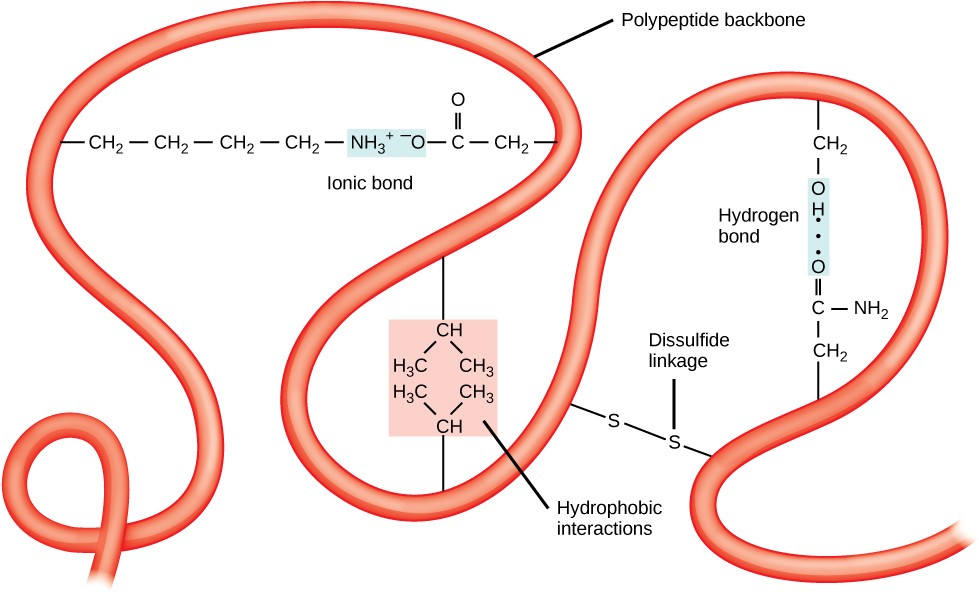
\includegraphics[width=13.6in]{/Users/nlb24/google_backup_sync_nlb24/lbrb/./images/protimage8} \caption{The tertiary structure of proteins is determined by a variety of chemical interactions. These include hydrophobic interactions, ionic bonding, hydrogen bonding and disulfide linkages.}\label{fig:unnamed-chunk-29}
\end{figure}

All of these interactions, weak and strong, determine the final
three-dimensional shape of the protein. When a protein loses its
three-dimensional shape, it may no longer be functional.

\hypertarget{quaternary-structure}{%
\subsection{Quaternary Structure}\label{quaternary-structure}}

In nature, some proteins are formed from several polypeptides, also
known as subunits, and the interaction of these subunits forms the
quaternary structure. Weak interactions between the subunits help to
stabilize the overall structure. For example, insulin (a globular
protein) has a combination of hydrogen bonds and disulfide bonds that
cause it to be mostly clumped into a ball shape. Insulin starts out as
a single polypeptide and loses some internal sequences in the presence
of post-translational modification after the formation of the
disulfide linkages that hold the remaining chains together. Silk (a
fibrous protein), however, has a \emph{β}-pleated sheet structure that is
the result of hydrogen bonding between different chains.

The four levels of protein structure (primary, secondary, tertiary,
and quaternary) are illustrated in Figure 3.4.9.

\begin{figure}
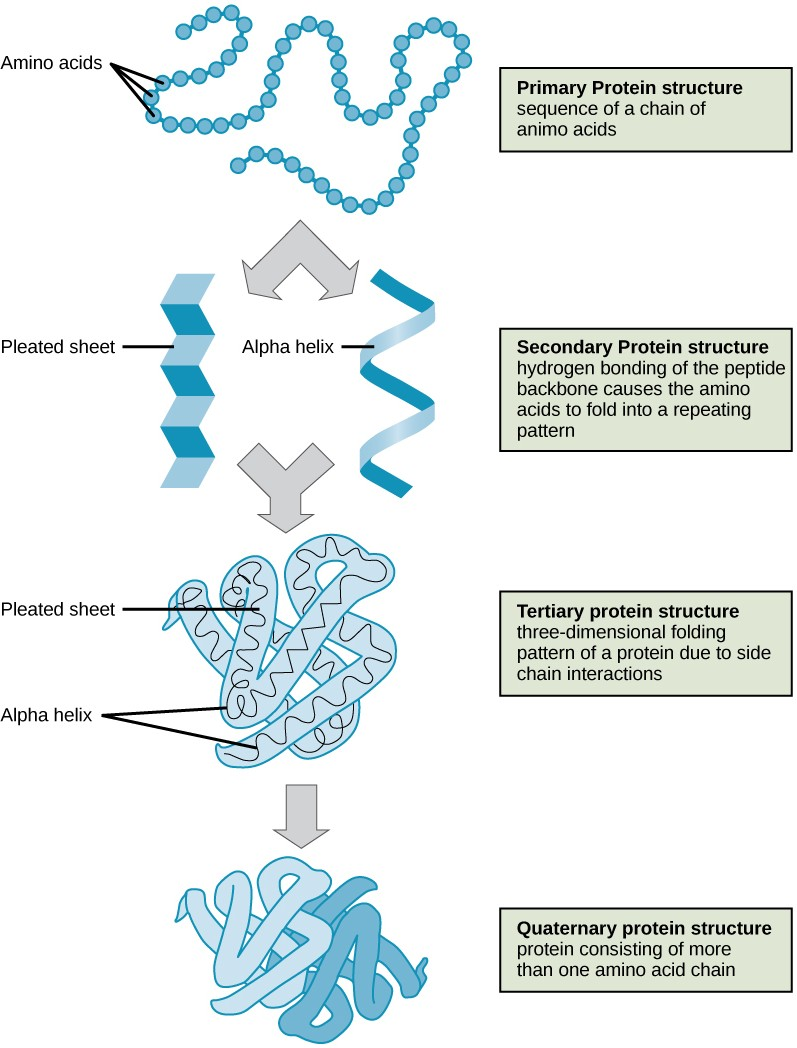
\includegraphics[width=11.07in]{/Users/nlb24/google_backup_sync_nlb24/lbrb/./images/protimage9} \caption{The four levels of protein structure can be observed in these illustrations. (credit: modification of work by National Human Genome Research Institute)}\label{fig:unnamed-chunk-30}
\end{figure}

\hypertarget{denaturation-and-protein-folding}{%
\section{Denaturation and Protein Folding}\label{denaturation-and-protein-folding}}

Each protein has its own unique sequence and shape that are held
together by chemical interactions. If the protein is subject to
changes in temperature, pH, or exposure to chemicals, the protein
structure may change, losing its shape without losing its primary
sequence in what is known as denaturation. Denaturation is often
reversible because the primary structure of the polypeptide is
conserved in the process if the denaturing agent is removed, allowing
the protein to resume its function. Sometimes denaturation is
irreversible, leading to loss of function. One example of irreversible
protein denaturation is when an egg is fried. The albumin protein in
the liquid egg white is denatured when placed in a hot pan. Not all
proteins are denatured at high temperatures; for instance, bacteria
that survive in hot springs have proteins that function at
temperatures close to boiling. The stomach is also very acidic, has a
low pH, and denatures proteins as part of the digestion process;
however, the digestive enzymes of the stomach retain their activity
under these conditions.

Protein folding is critical to its function. It was originally thought
that the proteins themselves were responsible for the folding process.
Only recently was it found that often they receive assistance in the
folding process from protein helpers known as chaperones (or
chaperonins) that associate with the target protein during the folding
process. They act by preventing aggregation of polypeptides that make
up the complete protein structure, and they disassociate from the
protein once the target protein is folded.

\hypertarget{summary-1}{%
\section{Summary}\label{summary-1}}

Proteins are a class of macromolecules that perform a diverse range of
functions for the cell. They help in metabolism by providing
structural support and by acting as enzymes, carriers, or hormones.
The building blocks of proteins (monomers) are amino acids. Each amino
acid has a central carbon that is linked to an amino group, a carboxyl
group, a hydrogen atom, and an

R group or side chain. There are 20 commonly occurring amino acids,
each of which differs in the R group. Each amino acid is linked to its
neighbors by a peptide bond. A long chain of amino acids is known as a
polypeptide.

Proteins are organized at four levels: primary, secondary, tertiary,
and (optional) quaternary. The primary structure is the unique
sequence of amino acids. The local folding of the polypeptide to form
structures such as the \emph{α} helix and \emph{β}-pleated sheet constitutes the
secondary structure. The overall three-dimensional structure is the
tertiary structure. When two or more polypeptides combine to form the
complete protein structure, the configuration is known as the
quaternary structure of a protein. Protein shape and function are
intricately linked; any change in shape caused by changes in
temperature or pH may lead to protein denaturation and a loss in
function.

\hypertarget{art-connections}{%
\section{Art Connections}\label{art-connections}}

\begin{itemize}
\item
  Which categories of amino acid would you expect to find on
  the surface of a soluble protein, and which would you expect to find
  in the interior? What distribution of amino acids would you expect to
  find in a protein embedded in a lipid bilayer?
\item
  Polar and charged amino acid residues (the remainder after
  peptide bond formation) are more likely to be found on the surface of
  soluble proteins where they can interact with water, and nonpolar
  (e.g., amino acid side chains) are more likely to be found in the
  interior where they are sequestered from water. In membrane proteins,
  nonpolar and hydrophobic amino acid side chains associate with the
  hydrophobic tails of phospholipids, while polar and charged amino acid
  side chains interact with the polar head groups or with the aqueous
  solution. However, there are exceptions. Sometimes, positively and
  negatively charged amino acid side chains interact with one another in
  the interior of a protein, and polar or charged amino acid side chains
  that interact with a ligand can be found in the ligand binding pocket.
\end{itemize}

\hypertarget{review-questions}{%
\section{Review Questions}\label{review-questions}}

The monomers that make up proteins are called
1. nucleotides
1. disaccharides
1. amino acids
1. chaperones

Answer: C

The \emph{α} helix and the \emph{β}-pleated sheet are part of which protein
structure?

\begin{enumerate}
\def\labelenumi{\arabic{enumi}.}
\tightlist
\item
  primary
\item
  secondary
\item
  tertiary
\item
  quaternary
\end{enumerate}

Answer: B

\hypertarget{free-response}{%
\section{Free Response}\label{free-response}}

\textbf{Explain what happens if even one amino acid is substituted for another
in a polypeptide chain. Provide a specific example.}

A change in gene sequence can lead to a different amino acid being
added to a polypeptide chain instead of the normal one. This causes a
change in protein structure and function. For example, in sickle cell
anemia, the hemoglobin \emph{β} chain has a single amino acid
substitution---the amino acid glutamic acid in position six is
substituted by valine. Because of this change, hemoglobin molecules
form aggregates, and the disc-shaped red blood cells assume a crescent
shape, which results in serious health problems.

\textbf{Describe the differences in the four protein structures.}

The sequence and number of amino acids in a polypeptide chain is its
primary structure. The local folding of the polypeptide in some
regions is the secondary structure of the protein. The
three-dimensional structure of a polypeptide is known as its tertiary
structure, created in part by chemical interactions such as hydrogen
bonds between polar side chains, van der Waals interactions, disulfide
linkages, and hydrophobic interactions. Some proteins are formed from
multiple polypeptides, also known as subunits, and the interaction of
these subunits forms the quaternary structure.

\hypertarget{glossary-1}{%
\section{Glossary}\label{glossary-1}}

\textbf{alpha-helix structure (\emph{α}-helix)}: type of secondary structure of proteins formed by folding of the polypeptide into a helix shape with hydrogen bonds stabilizing the
structure\\
\textbf{amino acid}: monomer of a protein; has a central carbon or alpha carbon to which an
amino group, a carboxyl group, a hydrogen, and an R group or side
chain is attached; the R group is different for all 20 amino acids\\
\textbf{beta-pleated sheet (\emph{β}-pleated)}: secondary structure found in proteins in which ``pleats'' are formed by hydrogen bonding between atoms on the backbone of the polypeptide chain\\
\textbf{chaperone}: (also, chaperonin) protein that helps nascent protein in the folding process \textbf{denaturation}: loss of shape in a protein as a result of changes in temperature, pH, or exposure to chemicals\\
\textbf{enzyme}: catalyst in a biochemical reaction that is usually a complex or conjugated protein\\
\textbf{hormone}: chemical signaling molecule, usually protein or steroid, secreted by endocrine cells that act to control or regulate specific physiological processes
\textbf{peptide bond}: bond formed between two amino acids by a dehydration reaction\\
\textbf{polypeptide}: long chain of amino acids linked by peptide bonds\\
\textbf{primary structure}: linear sequence of amino acids in a protein\\
\textbf{protein}: biological macromolecule composed of one or more chains of amino acids\\
\textbf{quaternary structure}: association of discrete polypeptide subunits in a protein\\
\textbf{secondary structure}: regular structure formed by proteins by intramolecular hydrogen bonding between the oxygen atom of one amino acid residue and the hydrogen attached to the nitrogen atom of another amino acid residue
\textbf{tertiary structure}: three-dimensional conformation of a protein, including interactions between secondary structural elements; formed from interactions between amino acid side chains

\hypertarget{contributors-and-attributions-1}{%
\section{Contributors and Attributions}\label{contributors-and-attributions-1}}

Connie Rye (East Mississippi Community College), Robert Wise
(University of Wisconsin, Oshkosh), Vladimir Jurukovski (Suffolk
County Community College), Jean DeSaix (University of North Carolina
at Chapel Hill), Jung Choi (Georgia Institute of Technology), Yael
Avissar (Rhode Island College) among other contributing authors.
Original content by OpenStax (CC BY 4.0; Download for free at
\href{http://cnx.org/contents/185cbf87-c72e-48f5-b51e-f14f21b5eabd\%409.87}{http://cnx.org/contents/185cbf87-c72...f21b5eabd@9.87}).

\hypertarget{downloading-r}{%
\chapter{Downloading R}\label{downloading-r}}

\textbf{By}: Avril Coghlan

\textbf{Adapted, edited and expanded}: Nathan Brouwer (\href{mailto:brouwern@gmail.com}{\nolinkurl{brouwern@gmail.com}}) under the Creative Commons 3.0 Attribution License \href{https://creativecommons.org/licenses/by/3.0/}{(CC BY 3.0)}.

\hypertarget{preface}{%
\section{Preface}\label{preface}}

The following introduction to \emph{R} is based on the first part of \href{https://a-little-book-of-r-for-bioinformatics.readthedocs.io/en/latest/src/installr.html}{``How to install \emph{R} and a Brief Introduction to R''} by Avril Coghlan, which was released under the Creative Commons 3.0 Attribution License \href{https://creativecommons.org/licenses/by/3.0/}{(CC BY 3.0)}. For additional information see the Appendices and \href{https://brouwern.github.io/BOOK_R_Ecological_Data_Science/getting-r-onto-your-computer.html}{``Getting \emph{R} onto your computer''}.

\hypertarget{introduction-to-r}{%
\section{Introduction to R}\label{introduction-to-r}}

\emph{R} (www.r-project.org) is a commonly used free statistics software. \emph{R} allows you to carry out statistical analyses in an interactive mode, as well as allowing programming.

\hypertarget{installing-r}{%
\section{Installing R}\label{installing-r}}

To use R, you first need to install the \emph{R} program on your computer.

\hypertarget{installing-r-on-a-windows-pc}{%
\subsection{\texorpdfstring{Installing \emph{R} on a Windows PC}{Installing R on a Windows PC}}\label{installing-r-on-a-windows-pc}}

These instructions will focus on installing \emph{R} on a Windows PC. However, I will also briefly mention how to install \emph{R} on a Macintosh or Linux computer (see below).

\textbf{These steps have not been checked as of 8/13/2019 so there may be small variations in what the prompts are. Installing R, however, is basically that same as any other program. Clicking ``Yes'' etc on everything should work.}

\begin{quote}
\textbf{PROTIP:} Even if you have used \emph{R} before its good to regularly update it to avoid conflicts with recently produced software.
\end{quote}

Minor updates of \emph{R} are made very regularly (approximately every 6 months), as \emph{R} is actively being improved all the time. It is worthwhile installing new versions of \emph{R} a couple times a year, to make sure that you have a recent version of \emph{R} (to ensure compatibility with all the latest versions of the \emph{R} packages that you have downloaded).

To install \emph{R} on your \textbf{Windows} computer, follow these steps:

\begin{enumerate}
\def\labelenumi{\arabic{enumi}.}
\tightlist
\item
  Go to \url{https://cran.r-project.org/}
\item
  Under ``Download and Install R'', click on the ``Windows'' link.
\item
  Under ``Subdirectories'', click on the \textbf{``base''} link.
\item
  On the next page, you should see a link saying something like ``Download \emph{R} 4.1.0 for Windows'' (or \emph{R} X.X.X, where X.X.X gives the version of the program). Click on this link.
\item
  You may be asked if you want to save or run a file ``R-x.x.x-win32.exe''. Choose ``Save'' and save the file. Then double-click on the icon for the file to run it.
\item
  You will be asked what language to install it in.
\item
  The \emph{R} Setup Wizard will appear in a window. Click ``Next'' at the bottom of the \emph{R} Setup wizard window.
\item
  The next page says ``Information'' at the top. Click ``Next'' again.
\item
  The next page says ``Select Destination Location'' at the top. By default, it will suggest to install \emph{R} on the C drive in the ``Program Files'' directory on your computer.
\item
  Click ``Next'' at the bottom of the \emph{R} Setup wizard window.
\item
  The next page says ``Select components'' at the top. Click ``Next'' again.
\item
  The next page says ``Startup options'' at the top. Click ``Next'' again.
\item
  The next page says ``Select start menu folder'' at the top. Click ``Next'' again.
\item
  The next page says ``Select additional tasks'' at the top. Click ``Next'' again.
\item
  \emph{R} should now be installing. This will take about a minute. When \emph{R} has finished, you will see ``Completing the \emph{R} for Windows Setup Wizard'' appear. Click ``Finish''.
\item
  To start R, you can do one of the following steps:
\item
  Check if there is an ``R'' icon on the desktop of the computer that you are using. If so, double-click on the ``R'' icon to start R. If you cannot find an ``R'' icon, try the next step instead.
\item
  Click on the ``Start'' button at the bottom left of your computer screen, and then choose ``All programs'', and start \emph{R} by selecting ``R'' (or \emph{R} X.X.X, where X.X.X gives the version of R) from the menu of programs.
\item
  The \emph{R} console (a rectangle) should pop up:
\end{enumerate}

\hypertarget{how-to-install-r-on-non-windows-computers-eg.-macintosh-or-linux-computers}{%
\subsection{\texorpdfstring{How to install \emph{R} on non-Windows computers (eg. Macintosh or Linux computers)}{How to install R on non-Windows computers (eg. Macintosh or Linux computers)}}\label{how-to-install-r-on-non-windows-computers-eg.-macintosh-or-linux-computers}}

\textbf{These steps have not been checked as of 8/13/2019 so there may be small variations in what the prompts are. Installing R, however, is basically that same as any other program. Clicking ``Yes'' etc on everything should work.}

The instructions above are for installing \emph{R} on a Windows PC. If you want to install \emph{R} on a computer that has a non-Windows operating system (for example, a Macintosh or computer running Linux, you should download the appropriate \emph{R} installer for that operating system at \url{https://cran.r-project.org/} and follow the \emph{R} installation instructions for the appropriate operating system at \url{https://cran.r-project.org/doc/FAQ/R-FAQ.html\#How-can-R-be-installed_003f} .

\hypertarget{starting-r}{%
\section{\texorpdfstring{Starting \emph{R}}{Starting R}}\label{starting-r}}

To start R, Check if there is an \emph{R} icon on the desktop of the computer that you are using. If so, double-click on the \emph{R} icon to start \emph{R}. If you cannot find an \emph{R} icon, try the next step instead.

You can also start \emph{R} from the Start menu in Windows. Click on the ``Start'' button at the bottom left of your computer screen, and then choose ``All programs'', and start \emph{R} by selecting ``R'' (or \emph{R} X.X.X, where X.X.X gives the version of R, e.g.. \emph{R} 2.10.0) from the menu of programs.

Say ``Hi'' to \emph{R} and take a quick look at how it looks. Now say ``Goodbye'', because we will never actually do any work in this version of \emph{R}; instead, we'll use the \textbf{RStudio IDE (integrated development environment)}.

\hypertarget{installing-the-rstudio-ide}{%
\chapter{Installing the RStudio IDE}\label{installing-the-rstudio-ide}}

\textbf{By:} Nathan Brouwer

The name ``R'' refers both to the programming language and the program that runs that language. When you download \emph{it}R* there is also a basic \textbf{GUI} (graphical user interface) that you can access via the \emph{R} icon.

Other GUIs are available, and the most popular currently is \textbf{RStudio.} RStudio a for-profit company that is a main driver of development of R. Much of what they produce has free basic versions or is entirely free. They produce software (RStudio), cloud-based applications (\textbf{RStudio Cloud}), and web server infrastructure for business applications of R.

A brief overview of installing RStudio can be found here \href{https://brouwern.github.io/BOOK_R_Ecological_Data_Science/getting-rstudio-on-to-your-computer.html}{``Getting RStudio on to your computer''}

\hypertarget{getting-to-know-rstudio}{%
\section{Getting to know RStudio}\label{getting-to-know-rstudio}}

For a brief overview of RStudio see \href{https://brouwern.github.io/BOOK_R_Ecological_Data_Science/getting-started-with-rstudio.html}{``Getting started with RStudio''}

A good overview of what the different parts of RStudio can be seen in the image in this tweet: \url{https://twitter.com/RLadiesNCL/status/1138812826917724160?s=20}

\hypertarget{rstudio-versus-rstudio-cloud}{%
\section{RStudio versus RStudio Cloud}\label{rstudio-versus-rstudio-cloud}}

RStudio and RStudio cloud work almost identically, so anything you read about RStudio will apply to RStudio Cloud. RStudio is easy to download an use, but RStudio Cloud eliminates even the minor hiccups that occur. Free accounts with RStudio Cloud allow up to 15 hours per month, which is enough for you to get a taste for using R.

\hypertarget{installing-r-packages}{%
\chapter{\texorpdfstring{Installing \emph{R} packages}{Installing R packages}}\label{installing-r-packages}}

\textbf{By}: Avril Coghlan.

\textbf{Adapted, edited and expanded}: Nathan Brouwer under the Creative Commons 3.0 Attribution License \href{https://creativecommons.org/licenses/by/3.0/}{(CC BY 3.0)}.

\emph{R} is a programming language, and \textbf{packages} (aka \textbf{libraries}) are bundles of software built using \emph{R}. Most sessions using \emph{R} involve using additional \emph{R} packages. This is especially true for bioinformatics and computational biology.

\begin{quote}
\textbf{NOTE}: If you are working in an RStudio Cloud environment organized by someone else (e.g.~a course instructor), they likely are taking care of many of the package management issues. The following information is still useful to be familiar with.
\end{quote}

\hypertarget{downloading-packages-with-the-rstudio-ide}{%
\section{Downloading packages with the RStudio IDE}\label{downloading-packages-with-the-rstudio-ide}}

There is a point-and-click interface for installing \emph{R} packages in RStudio. There is a brief introduction to downloading packages on this site: \url{http://web.cs.ucla.edu/~gulzar/rstudio/}

I've summarized it here:

\begin{enumerate}
\def\labelenumi{\arabic{enumi}.}
\tightlist
\item
  ``Click on the''Packages'' tab in the bottom-right section and then click on ``Install''. The following dialog box will appear.
\item
  In the ``Install Packages'' dialog, write the package name you want to install under the Packages field and then click install. This will install the package you searched for or give you a list of matching package based on your package text.
\end{enumerate}

\hypertarget{downloading-packages-with-the-function-install.packages}{%
\section{\texorpdfstring{Downloading packages with the function \texttt{install.packages()}}{Downloading packages with the function install.packages()}}\label{downloading-packages-with-the-function-install.packages}}

The easiest way to install a package if you know its name is to use the \emph{R} function \texttt{install.packages(})`. Note that it might be better to call this ``download.packages'' since after you install it, you also have to load it!

Frequently I will include \texttt{install.packages(...)} at the beginning of a chapter the first time we use a package to make sure the package is downloaded. Note, however, that if you already have downloaded the package, running \texttt{install.packages(...)} will download a new copy. While packages do get updated from time to time, but its best to re-run \texttt{install.packages(...)} only occassionaly.

We'll download a package used for plotting called \texttt{ggplot2}, which stands for ``Grammar of Graphics.'' \texttt{ggplot2} was developed by Dr.~\href{http://hadley.nz/}{Hadley Wickham}, who is now the Chief Scientists for RStudio.

To download \texttt{ggplot2}, run the following command:

\begin{Shaded}
\begin{Highlighting}[]
\FunctionTok{install.packages}\NormalTok{(}\StringTok{"ggplot2"}\NormalTok{) }\CommentTok{\# note the " "}
\end{Highlighting}
\end{Shaded}

Often when you download a package you'll see a fair bit of angry-looking red text, and sometime other things will pop up. Usually there's nothing of interest here, but sometimes you need to read things carefully over it for hints about why something didn't work.

\hypertarget{using-packages-after-they-are-downloaded}{%
\section{Using packages after they are downloaded}\label{using-packages-after-they-are-downloaded}}

To actually make the functions in package accessible you need to use the \texttt{library()} command. Note that this is \emph{not} in quotes.

\begin{Shaded}
\begin{Highlighting}[]
\FunctionTok{library}\NormalTok{(ggplot2) }\CommentTok{\# note: NO " "}
\end{Highlighting}
\end{Shaded}

\hypertarget{installing-bioconductor}{%
\chapter{Installing Bioconductor}\label{installing-bioconductor}}

\textbf{By}: Avril Coghlan.

\textbf{Adapted, edited and expanded}: Nathan Brouwer under the Creative Commons 3.0 Attribution License \href{https://creativecommons.org/licenses/by/3.0/}{(CC BY 3.0)}, including details on install Bioconductor and common prompts and error messages that appear during installation.

\hypertarget{bioconductor}{%
\section{Bioconductor}\label{bioconductor}}

\emph{R} \textbf{packages} (aka ``libraries'') can live in many places. Most are accessed via \textbf{CRAN}, the \textbf{Comprehensive R Archive Network}. The bioinformatics and computational biology community also has its own package hosting system called \href{www.bioconductor.org}{Bioconductor}. \emph{R} has played an important part in the development and application of bioinformatics techniques in the 21th century. Bioconductor 1.0 was released in 2002 with 15 packages. As of winter 2021, there are almost 2000 packages in the current release!

\begin{quote}
\textbf{NOTE}: If you are working in an RStudio Cloud environment organized by someone else (eg a course instructor), they likely are taking care of most of package management issues, inlcuding setting up Bioconductor. The following information is still useful to be familiar with.
\end{quote}

To interface with Bioconductor you need the \href{https://cran.r-project.org/web/packages/BiocManager/vignettes/BiocManager.html}{BiocManager} package. The Bioconductor people have put \href{https://cran.r-project.org/web/packages/BiocManager/vignettes/BiocManager.html}{BiocManager} on CRAN to allow you to set up interactions with Bioconductor. See the \href{https://cran.r-project.org/web/packages/BiocManager/vignettes/BiocManager.html}{BiocManager documentation} for more information (\url{https://cran.r-project.org/web/packages/BiocManager/vignettes/BiocManager.html}).

Note that if you have an old version of R you will need to update it to interact with Bioconductor.

\hypertarget{installing-biocmanager}{%
\section{Installing BiocManager}\label{installing-biocmanager}}

BiocManager can be installed using the \texttt{install.packages()} packages command.

\begin{Shaded}
\begin{Highlighting}[]
\FunctionTok{install.packages}\NormalTok{(}\StringTok{"BiocManager"}\NormalTok{) }\CommentTok{\# Remember the "  "; don\textquotesingle{}t worry about the red text}
\end{Highlighting}
\end{Shaded}

Once downloaded, BioManager needs to be explicitly loaded into your active R session using \texttt{library()}

\begin{Shaded}
\begin{Highlighting}[]
\FunctionTok{library}\NormalTok{(BiocManager) }\CommentTok{\# no quotes; again, ignore the red text}
\end{Highlighting}
\end{Shaded}

Individual Bioconductor packages can then be downloaded using the \texttt{install()} command. An essential packages is \texttt{Biostrings}. To do this ,

\begin{Shaded}
\begin{Highlighting}[]
\NormalTok{BiocManager}\SpecialCharTok{::}\FunctionTok{install}\NormalTok{(}\StringTok{"Biostrings"}\NormalTok{)}
\end{Highlighting}
\end{Shaded}

\hypertarget{the-ins-and-outs-of-package-installation}{%
\section{The ins and outs of package installation}\label{the-ins-and-outs-of-package-installation}}

\textbf{IMPORANT} Bioconductor has many \textbf{dependencies} - other packages which is relies on. When you install Bioconductor packages you may need to update these packages. If something seems to not be working during this process, restart R and begin the Bioconductor installation process until things seem to work.

Below I discuss the series of prompts I had to deal with while re-installing Biostrings while editing this chapter.

\hypertarget{updating-other-packages-when-downloading-a-package}{%
\subsection{Updating other packages when downloading a package}\label{updating-other-packages-when-downloading-a-package}}

When I re-installed \texttt{Biostrings} while writing this I was given a HUGE blog of red test that contained this:

\begin{Shaded}
\begin{Highlighting}[]
\StringTok{\textquotesingle{}getOption("repos")\textquotesingle{}}\NormalTok{ replaces Bioconductor standard repositories, see }\StringTok{\textquotesingle{}?repositories\textquotesingle{}} \ControlFlowTok{for}
\NormalTok{details}

\NormalTok{replacement repositories}\SpecialCharTok{:}
\NormalTok{    CRAN}\SpecialCharTok{:}\NormalTok{ https}\SpecialCharTok{:}\ErrorTok{//}\NormalTok{cran.rstudio.com}\SpecialCharTok{/}

\NormalTok{Bioconductor version }\FloatTok{3.11}\NormalTok{ (BiocManager }\DecValTok{1}\NormalTok{.}\FloatTok{30.16}\NormalTok{), R }\DecValTok{4}\NormalTok{.}\FloatTok{0.5}\NormalTok{ (}\DecValTok{2021{-}03{-}31}\NormalTok{)}
\NormalTok{Old packages}\SpecialCharTok{:} \StringTok{\textquotesingle{}ade4\textquotesingle{}}\NormalTok{, }\StringTok{\textquotesingle{}ape\textquotesingle{}}\NormalTok{, }\StringTok{\textquotesingle{}aster\textquotesingle{}}\NormalTok{, }\StringTok{\textquotesingle{}bayestestR\textquotesingle{}}\NormalTok{, }\StringTok{\textquotesingle{}bio3d\textquotesingle{}}\NormalTok{, }\StringTok{\textquotesingle{}bitops\textquotesingle{}}\NormalTok{, }\StringTok{\textquotesingle{}blogdown\textquotesingle{}}\NormalTok{,}
  \StringTok{\textquotesingle{}bookdown\textquotesingle{}}\NormalTok{, }\StringTok{\textquotesingle{}brio\textquotesingle{}}\NormalTok{, }\StringTok{\textquotesingle{}broom\textquotesingle{}}\NormalTok{, }\StringTok{\textquotesingle{}broom.mixed\textquotesingle{}}\NormalTok{, }\StringTok{\textquotesingle{}broomExtra\textquotesingle{}}\NormalTok{, }\StringTok{\textquotesingle{}bslib\textquotesingle{}}\NormalTok{, }\StringTok{\textquotesingle{}cachem\textquotesingle{}}\NormalTok{, }\StringTok{\textquotesingle{}callr\textquotesingle{}}\NormalTok{,}
  \StringTok{\textquotesingle{}car\textquotesingle{}}\NormalTok{, }\StringTok{\textquotesingle{}circlize\textquotesingle{}}\NormalTok{, }\StringTok{\textquotesingle{}class\textquotesingle{}}\NormalTok{, }\StringTok{\textquotesingle{}cli\textquotesingle{}}\NormalTok{, }\StringTok{\textquotesingle{}cluster\textquotesingle{}}\NormalTok{, }\StringTok{\textquotesingle{}colorspace\textquotesingle{}}\NormalTok{, }\StringTok{\textquotesingle{}corrplot\textquotesingle{}}\NormalTok{, }\StringTok{\textquotesingle{}cpp11\textquotesingle{}}\NormalTok{, }\StringTok{\textquotesingle{}curl\textquotesingle{}}\NormalTok{,}
  \StringTok{\textquotesingle{}devtools\textquotesingle{}}\NormalTok{, }\StringTok{\textquotesingle{}DHARMa\textquotesingle{}}\NormalTok{, }\StringTok{\textquotesingle{}doBy\textquotesingle{}}\NormalTok{, }\StringTok{\textquotesingle{}dplyr\textquotesingle{}}\NormalTok{, }\StringTok{\textquotesingle{}DT\textquotesingle{}}\NormalTok{, }\StringTok{\textquotesingle{}e1071\textquotesingle{}}\NormalTok{, }\StringTok{\textquotesingle{}ellipsis\textquotesingle{}}\NormalTok{, }\StringTok{\textquotesingle{}emmeans\textquotesingle{}}\NormalTok{, }\StringTok{\textquotesingle{}emojifont\textquotesingle{}}\NormalTok{,}
  \StringTok{\textquotesingle{}extRemes\textquotesingle{}}\NormalTok{, }\StringTok{\textquotesingle{}fansi\textquotesingle{}}\NormalTok{, }\StringTok{\textquotesingle{}flextable\textquotesingle{}}\NormalTok{, }\StringTok{\textquotesingle{}forecast\textquotesingle{}}\NormalTok{, }\StringTok{\textquotesingle{}formatR\textquotesingle{}}\NormalTok{, }\StringTok{\textquotesingle{}gap\textquotesingle{}}\NormalTok{, }\StringTok{\textquotesingle{}gargle\textquotesingle{}}\NormalTok{, }\StringTok{\textquotesingle{}gert\textquotesingle{}}\NormalTok{, }\StringTok{\textquotesingle{}GGally\textquotesingle{}}\NormalTok{,}
  \StringTok{\textquotesingle{}ggfortify\textquotesingle{}}\NormalTok{, }\StringTok{\textquotesingle{}ggplot2\textquotesingle{}}\NormalTok{, }\StringTok{\textquotesingle{}ggsignif\textquotesingle{}}\NormalTok{, }\StringTok{\textquotesingle{}ggVennDiagram\textquotesingle{}}\NormalTok{, }\StringTok{\textquotesingle{}gh\textquotesingle{}}\NormalTok{, }\StringTok{\textquotesingle{}glmmTMB\textquotesingle{}}\NormalTok{, }\StringTok{\textquotesingle{}googledrive\textquotesingle{}}\NormalTok{,}
  \StringTok{\textquotesingle{}gtools\textquotesingle{}}\NormalTok{, }\StringTok{\textquotesingle{}haven\textquotesingle{}}\NormalTok{, }\StringTok{\textquotesingle{}highr\textquotesingle{}}\NormalTok{, }\StringTok{\textquotesingle{}hms\textquotesingle{}}\NormalTok{, }\StringTok{\textquotesingle{}htmlTable\textquotesingle{}}\NormalTok{, }\StringTok{\textquotesingle{}httpuv\textquotesingle{}}\NormalTok{, }\StringTok{\textquotesingle{}huxtable\textquotesingle{}}\NormalTok{, }\StringTok{\textquotesingle{}jquerylib\textquotesingle{}}\NormalTok{,}
  \StringTok{\textquotesingle{}KernSmooth\textquotesingle{}}\NormalTok{, }\StringTok{\textquotesingle{}knitr\textquotesingle{}}\NormalTok{, }\StringTok{\textquotesingle{}later\textquotesingle{}}\NormalTok{, }\StringTok{\textquotesingle{}lattice\textquotesingle{}}\NormalTok{, }\StringTok{\textquotesingle{}lme4\textquotesingle{}}\NormalTok{, }\StringTok{\textquotesingle{}magick\textquotesingle{}}\NormalTok{, }\StringTok{\textquotesingle{}manipulateWidget\textquotesingle{}}\NormalTok{, }\StringTok{\textquotesingle{}MASS\textquotesingle{}}\NormalTok{,}
  \StringTok{\textquotesingle{}Matrix\textquotesingle{}}\NormalTok{, }\StringTok{\textquotesingle{}matrixcalc\textquotesingle{}}\NormalTok{, }\StringTok{\textquotesingle{}matrixStats\textquotesingle{}}\NormalTok{, }\StringTok{\textquotesingle{}mgcv\textquotesingle{}}\NormalTok{, }\StringTok{\textquotesingle{}mime\textquotesingle{}}\NormalTok{, }\StringTok{\textquotesingle{}multcomp\textquotesingle{}}\NormalTok{, }\StringTok{\textquotesingle{}mvtnorm\textquotesingle{}}\NormalTok{, }\StringTok{\textquotesingle{}nnet\textquotesingle{}}\NormalTok{,}
  \StringTok{\textquotesingle{}openssl\textquotesingle{}}\NormalTok{, }\StringTok{\textquotesingle{}openxlsx\textquotesingle{}}\NormalTok{, }\StringTok{\textquotesingle{}parameters\textquotesingle{}}\NormalTok{, }\StringTok{\textquotesingle{}pBrackets\textquotesingle{}}\NormalTok{, }\StringTok{\textquotesingle{}pdftools\textquotesingle{}}\NormalTok{, }\StringTok{\textquotesingle{}phangorn\textquotesingle{}}\NormalTok{, }\StringTok{\textquotesingle{}phytools\textquotesingle{}}\NormalTok{,}
  \StringTok{\textquotesingle{}pillar\textquotesingle{}}\NormalTok{, }\StringTok{\textquotesingle{}plotly\textquotesingle{}}\NormalTok{, }\StringTok{\textquotesingle{}processx\textquotesingle{}}\NormalTok{, }\StringTok{\textquotesingle{}proxy\textquotesingle{}}\NormalTok{, }\StringTok{\textquotesingle{}qgam\textquotesingle{}}\NormalTok{, }\StringTok{\textquotesingle{}quantreg\textquotesingle{}}\NormalTok{, }\StringTok{\textquotesingle{}ragg\textquotesingle{}}\NormalTok{, }\StringTok{\textquotesingle{}Rcpp\textquotesingle{}}\NormalTok{,}
  \StringTok{\textquotesingle{}RcppArmadillo\textquotesingle{}}\NormalTok{, }\StringTok{\textquotesingle{}remotes\textquotesingle{}}\NormalTok{, }\StringTok{\textquotesingle{}rgl\textquotesingle{}}\NormalTok{, }\StringTok{\textquotesingle{}rio\textquotesingle{}}\NormalTok{, }\StringTok{\textquotesingle{}rJava\textquotesingle{}}\NormalTok{, }\StringTok{\textquotesingle{}rlang\textquotesingle{}}\NormalTok{, }\StringTok{\textquotesingle{}rmarkdown\textquotesingle{}}\NormalTok{, }\StringTok{\textquotesingle{}robustbase\textquotesingle{}}\NormalTok{,}
  \StringTok{\textquotesingle{}rsconnect\textquotesingle{}}\NormalTok{, }\StringTok{\textquotesingle{}rversions\textquotesingle{}}\NormalTok{, }\StringTok{\textquotesingle{}sandwich\textquotesingle{}}\NormalTok{, }\StringTok{\textquotesingle{}sass\textquotesingle{}}\NormalTok{, }\StringTok{\textquotesingle{}segmented\textquotesingle{}}\NormalTok{, }\StringTok{\textquotesingle{}seqinr\textquotesingle{}}\NormalTok{, }\StringTok{\textquotesingle{}seqmagick\textquotesingle{}}\NormalTok{, }\StringTok{\textquotesingle{}servr\textquotesingle{}}\NormalTok{,}
  \StringTok{\textquotesingle{}sf\textquotesingle{}}\NormalTok{, }\StringTok{\textquotesingle{}shape\textquotesingle{}}\NormalTok{, }\StringTok{\textquotesingle{}spatial\textquotesingle{}}\NormalTok{, }\StringTok{\textquotesingle{}statmod\textquotesingle{}}\NormalTok{, }\StringTok{\textquotesingle{}stringi\textquotesingle{}}\NormalTok{, }\StringTok{\textquotesingle{}systemfonts\textquotesingle{}}\NormalTok{, }\StringTok{\textquotesingle{}testthat\textquotesingle{}}\NormalTok{, }\StringTok{\textquotesingle{}textshaping\textquotesingle{}}\NormalTok{,}
  \StringTok{\textquotesingle{}tibble\textquotesingle{}}\NormalTok{, }\StringTok{\textquotesingle{}tidyselect\textquotesingle{}}\NormalTok{, }\StringTok{\textquotesingle{}tidytree\textquotesingle{}}\NormalTok{, }\StringTok{\textquotesingle{}tinytex\textquotesingle{}}\NormalTok{, }\StringTok{\textquotesingle{}tufte\textquotesingle{}}\NormalTok{, }\StringTok{\textquotesingle{}UniprotR\textquotesingle{}}\NormalTok{, }\StringTok{\textquotesingle{}units\textquotesingle{}}\NormalTok{, }\StringTok{\textquotesingle{}vctrs\textquotesingle{}}\NormalTok{,}
  \StringTok{\textquotesingle{}viridis\textquotesingle{}}\NormalTok{, }\StringTok{\textquotesingle{}viridisLite\textquotesingle{}}\NormalTok{, }\StringTok{\textquotesingle{}withr\textquotesingle{}}\NormalTok{, }\StringTok{\textquotesingle{}xfun\textquotesingle{}}\NormalTok{, }\StringTok{\textquotesingle{}zip\textquotesingle{}}
\end{Highlighting}
\end{Shaded}

Hidden at the bottom was a prompt: ``Update all/some/none? {[}a/s/n{]}:''

Its a little vague, but what it wants me to do is type in a, s or n and press enter to tell it what to do. I almost always chose ``a'', though this may take a while to update everything.

\hypertarget{packages-from-source}{%
\subsection{Packages ``from source''}\label{packages-from-source}}

You are likely to get lots of random-looking feedback from R when doing Bioconductor-related installations. Look carefully for any prompts as the very last line. While updating \texttt{Biostrings} I was told: ``\emph{There are binary versions available but the source versions are later:}'' and given a table of packages. I was then asked ``\emph{Do you want to install from sources the packages which need compilation? (Yes/no/cancel)}''

I almost always chose ``no''.

\hypertarget{more-on-angry-red-text}{%
\subsection{More on angry red text}\label{more-on-angry-red-text}}

After the prompt about packages from source, R proceeded to download a lot of updates to packages, which took a few minutes. Lots of red text scrolled by, but this is normal.

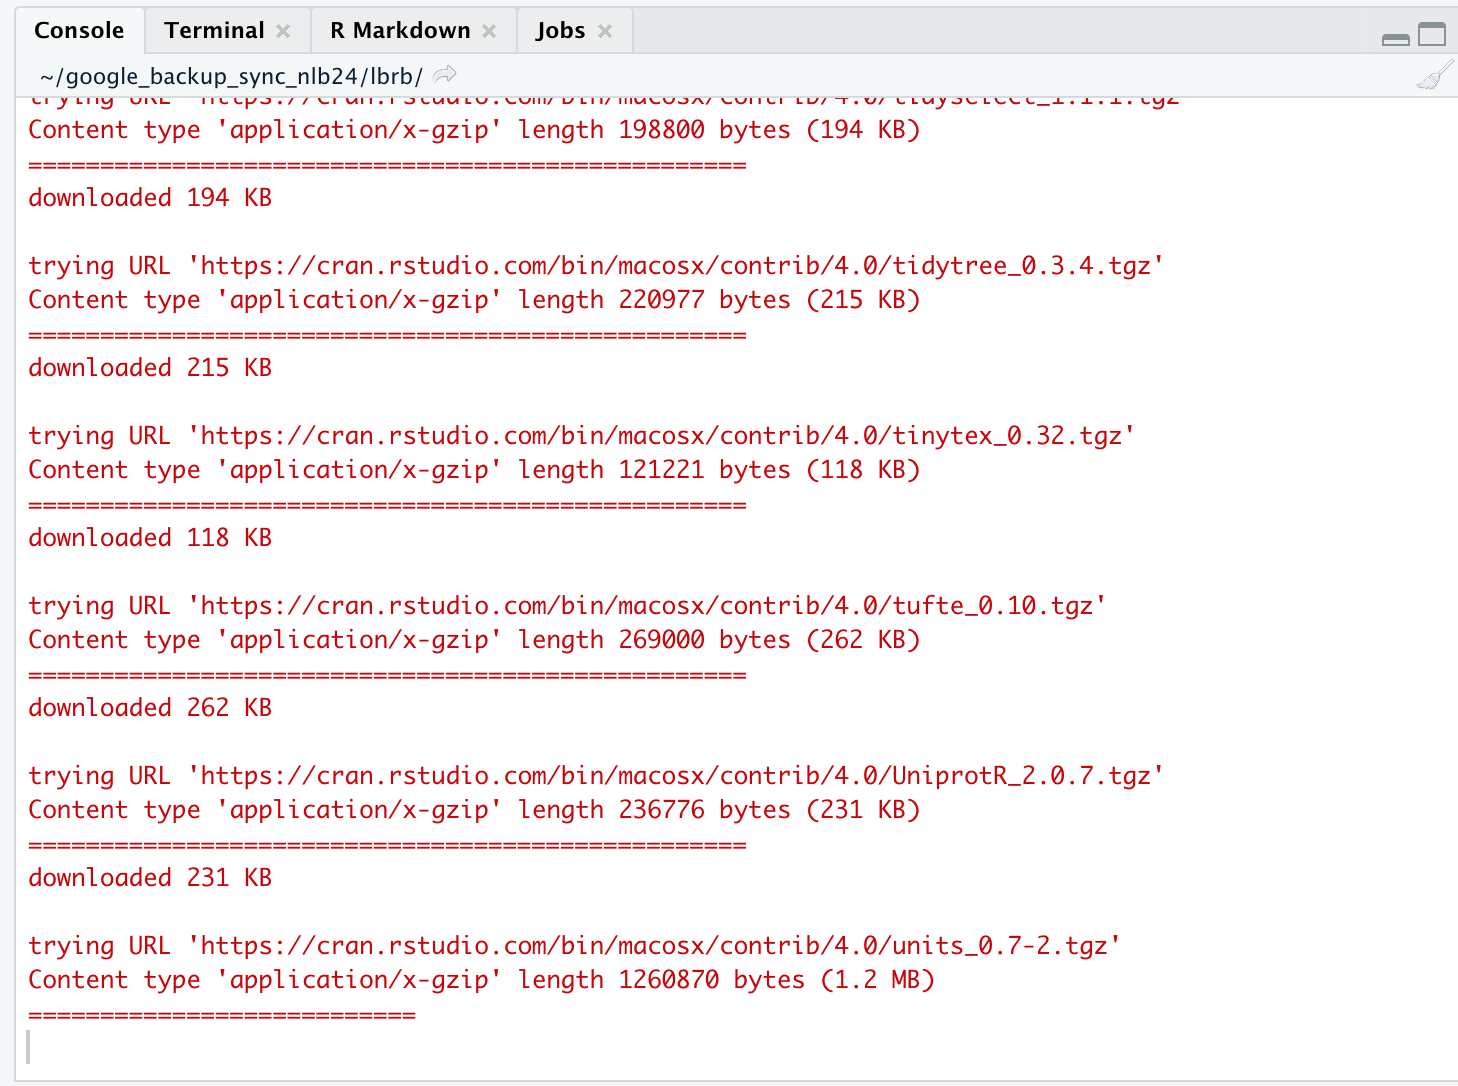
\includegraphics[width=20.25in]{images/angry_red_text_download_biostrings}

\hypertarget{actually-loading-a-package}{%
\section{Actually loading a package}\label{actually-loading-a-package}}

Again, to actually load the \texttt{Biostrings} package into your active R sessions requires the \texttt{libary()} command:

\begin{Shaded}
\begin{Highlighting}[]
\FunctionTok{library}\NormalTok{(Biostrings)}
\end{Highlighting}
\end{Shaded}

As you might expect, there's more red text scrolling up my screen!

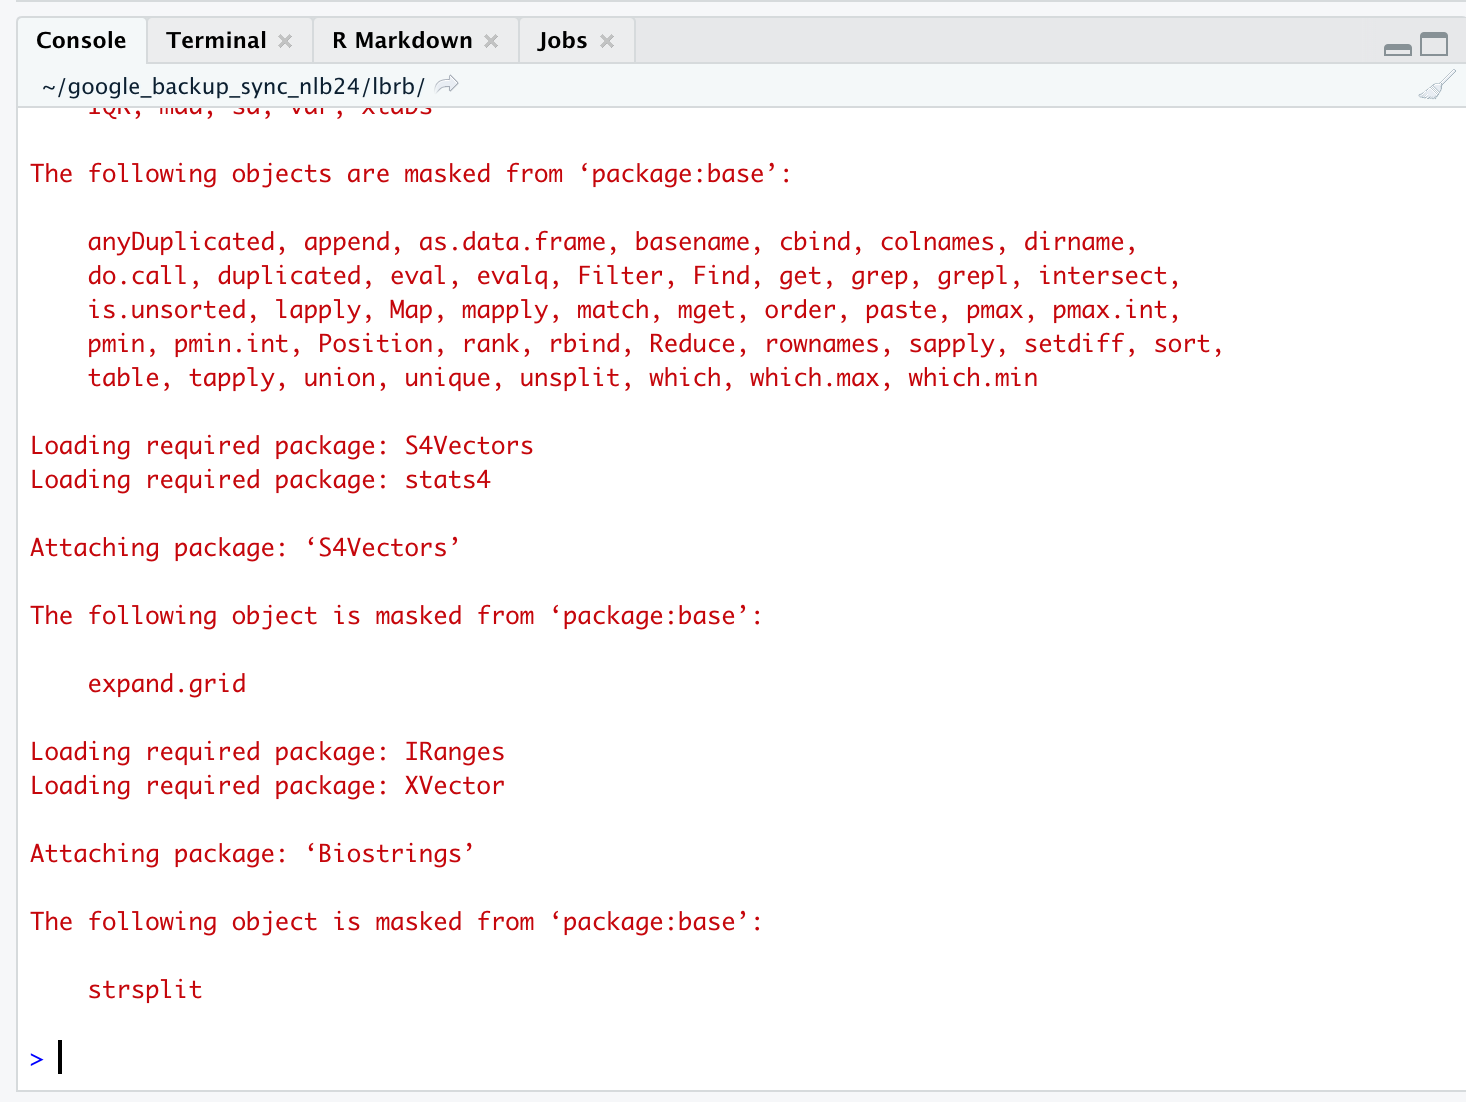
\includegraphics[width=20.36in]{images/angry_red_text_library_biostrings}

I can tell that is actually worked because at the end of all the red stuff is the R prompt of ``\textgreater{}'' and my cursor.


\includegraphics[width=1.42in]{images/R_cursor}

\hypertarget{a-brief-introduction-to-r}{%
\chapter{A Brief introduction to R}\label{a-brief-introduction-to-r}}

\textbf{By}: Avril Coghlan.

\textbf{Adapted, edited and expanded}: Nathan Brouwer under the Creative Commons 3.0 Attribution License \href{https://creativecommons.org/licenses/by/3.0/}{(CC BY 3.0)}.

This chapter provides a brief introduction to R. At the end of are links to additional resources for getting started with R.

\hypertarget{vocabulary}{%
\section{Vocabulary}\label{vocabulary}}

\begin{itemize}
\tightlist
\item
  scalar
\item
  vector
\item
  list
\item
  class
\item
  numeric
\item
  character
\item
  assignment
\item
  elements of an object
\item
  indices
\item
  attributes of an object
\item
  argument of a function
\end{itemize}

\hypertarget{r-functions}{%
\section{R functions}\label{r-functions}}

\begin{itemize}
\tightlist
\item
  \textless-
\item
  {[} {]}
\item
  \$
\item
  table()
\item
  function
\item
  c()
\item
  log10()
\item
  help(), ?
\item
  help.search()
\item
  RSiteSearch()
\item
  mean()
\item
  return()
\item
  q()
\end{itemize}

\hypertarget{interacting-with-r}{%
\section{Interacting with R}\label{interacting-with-r}}

You will type \emph{R} commands into the RStudio \textbf{console} in order to carry out analyses in \emph{R}. In the RStudio console you will see the R prompt starting with the symbol ``\textgreater{}''. ``\textgreater{}'' will always be there at the beginning of each new command - don't try to delete it! Moreover, you never need to type it.


\includegraphics[width=1.42in]{images/R_cursor}

We type the \textbf{commands} needed for a particular task after this prompt. The command is carried out by \emph{R} after you hit the Return key.

Once you have started R, you can start typing commands into the RStudio console, and the results will be calculated immediately, for example:

\begin{Shaded}
\begin{Highlighting}[]
\DecValTok{2}\SpecialCharTok{*}\DecValTok{3}
\end{Highlighting}
\end{Shaded}

\begin{verbatim}
## [1] 6
\end{verbatim}

Note that prior to the output of ``6'' it shows ``{[}1{]}''.

Now subtraction:

\begin{Shaded}
\begin{Highlighting}[]
\DecValTok{10{-}3}
\end{Highlighting}
\end{Shaded}

\begin{verbatim}
## [1] 7
\end{verbatim}

Again, prior to the output of ``7'' it shows ``{[}1{]}''.

\emph{R} can act like a basic calculator that you type commands in to. You can also use it like a more advanced scientific calculator and create \textbf{variables} that store information. All variables created by R are called \textbf{objects}. In R, we assign values to variables using an arrow-looking function \texttt{\textless{}-} the \textbf{assignment operator}. For example, we can \textbf{assign} the value 2*3 to the variable x using the command:

\begin{Shaded}
\begin{Highlighting}[]
\NormalTok{x }\OtherTok{\textless{}{-}} \DecValTok{2}\SpecialCharTok{*}\DecValTok{3}
\end{Highlighting}
\end{Shaded}

To view the contents of any R object, just type its name, press enter, and the contents of that R object will be displayed:

\begin{Shaded}
\begin{Highlighting}[]
\NormalTok{x}
\end{Highlighting}
\end{Shaded}

\begin{verbatim}
## [1] 6
\end{verbatim}

\hypertarget{variables-in-r}{%
\section{Variables in R}\label{variables-in-r}}

There are several different types of objects in R with fancy math names, including \textbf{scalars}, \textbf{vectors}, \textbf{matrices} (singular: \textbf{matrix), }arrays\textbf{, }dataframes\textbf{, }tables\textbf{, and }lists\textbf{. The }scalar** variable x above is one example of an R object. While a scalar variable such as x has just one element, a \textbf{vector} consists of several elements. The elements in a vector are all of the same \textbf{type} (e.g.. numbers or alphabetic characters), while \textbf{lists} may include elements such as characters as well as numeric quantities. Vectors and dataframes are the most common variables you'll use. You'll also encounter matrices often, and lists are ubiquitous in R but beginning users often don't encounter them because they remain behind the scenes.

\hypertarget{vectors}{%
\subsection{Vectors}\label{vectors}}

To create a vector, we can use the \texttt{c()} (combine) function. For example, to create a vector called \texttt{myvector} that has elements with values 8, 6, 9, 10, and 5, we type:

\begin{Shaded}
\begin{Highlighting}[]
\NormalTok{myvector }\OtherTok{\textless{}{-}} \FunctionTok{c}\NormalTok{(}\DecValTok{8}\NormalTok{, }\DecValTok{6}\NormalTok{, }\DecValTok{9}\NormalTok{, }\DecValTok{10}\NormalTok{, }\DecValTok{5}\NormalTok{) }\CommentTok{\# note: commas between each number!}
\end{Highlighting}
\end{Shaded}

To see the contents of the variable \texttt{myvector}, we can just type its name and press enter:

\begin{Shaded}
\begin{Highlighting}[]
\NormalTok{myvector}
\end{Highlighting}
\end{Shaded}

\begin{verbatim}
## [1]  8  6  9 10  5
\end{verbatim}

\hypertarget{vector-indexing}{%
\subsection{Vector indexing}\label{vector-indexing}}

The \texttt{{[}1{]}} is the \textbf{index} of the first \textbf{element} in the vector. We can \textbf{extract} any element of the vector by typing the vector name with the index of that element given in \textbf{square brackets} \texttt{{[}...{]}}.

For example, to get the value of the 4th element in the vector \texttt{myvector}, we type:

\begin{Shaded}
\begin{Highlighting}[]
\NormalTok{myvector[}\DecValTok{4}\NormalTok{]}
\end{Highlighting}
\end{Shaded}

\begin{verbatim}
## [1] 10
\end{verbatim}

\hypertarget{character-vectors}{%
\subsection{Character vectors}\label{character-vectors}}

Vectors can contain letters, such as those designating nucleic acids

\begin{Shaded}
\begin{Highlighting}[]
\NormalTok{my.seq }\OtherTok{\textless{}{-}} \FunctionTok{c}\NormalTok{(}\StringTok{"A"}\NormalTok{,}\StringTok{"T"}\NormalTok{,}\StringTok{"C"}\NormalTok{,}\StringTok{"G"}\NormalTok{)}
\end{Highlighting}
\end{Shaded}

They can also contain multi-letter \textbf{strings}:

\begin{Shaded}
\begin{Highlighting}[]
\NormalTok{my.oligos }\OtherTok{\textless{}{-}} \FunctionTok{c}\NormalTok{(}\StringTok{"ATCGC"}\NormalTok{,}\StringTok{"TTTCGC"}\NormalTok{,}\StringTok{"CCCGCG"}\NormalTok{,}\StringTok{"GGGCGC"}\NormalTok{)}
\end{Highlighting}
\end{Shaded}

\hypertarget{lists}{%
\subsection{Lists}\label{lists}}

\textbf{NOTE}: \emph{below is a discussion of lists in R. This is excellent information, but not necessary if this is your very very first time using R.}

In contrast to a vector, a \textbf{list} can contain elements of different types, for example, both numbers and letters. A list can even include other variables such as a vector. The \texttt{list()} function is used to create a list. For example, we could create a list \texttt{mylist} by typing:

\begin{Shaded}
\begin{Highlighting}[]
\NormalTok{mylist }\OtherTok{\textless{}{-}} \FunctionTok{list}\NormalTok{(}\AttributeTok{name=}\StringTok{"Charles Darwin"}\NormalTok{, }
               \AttributeTok{wife=}\StringTok{"Emma Darwin"}\NormalTok{, }
\NormalTok{               myvector)}
\end{Highlighting}
\end{Shaded}

We can then print out the contents of the list mylist by typing its name:

\begin{Shaded}
\begin{Highlighting}[]
\NormalTok{mylist}
\end{Highlighting}
\end{Shaded}

\begin{verbatim}
## $name
## [1] "Charles Darwin"
## 
## $wife
## [1] "Emma Darwin"
## 
## [[3]]
## [1]  8  6  9 10  5
\end{verbatim}

The \textbf{elements} in a list are numbered, and can be referred to using \textbf{indices}. We can extract an element of a list by typing the list name with the index of the element given in double \textbf{square brackets} (in contrast to a vector, where we only use single square brackets).

We can extract the second element from \texttt{mylist} by typing:

\begin{Shaded}
\begin{Highlighting}[]
\NormalTok{mylist[[}\DecValTok{2}\NormalTok{]]  }\CommentTok{\# note the double square brackets [[...]]}
\end{Highlighting}
\end{Shaded}

\begin{verbatim}
## [1] "Emma Darwin"
\end{verbatim}

As a baby step towards our next task, we can wrap index values as in the \texttt{c()} command like this:

\begin{Shaded}
\begin{Highlighting}[]
\NormalTok{mylist[[}\FunctionTok{c}\NormalTok{(}\DecValTok{2}\NormalTok{)]]  }\CommentTok{\# note the double square brackets [[...]]}
\end{Highlighting}
\end{Shaded}

\begin{verbatim}
## [1] "Emma Darwin"
\end{verbatim}

The number \texttt{2} and \texttt{c(2)} mean the same thing.

Now, we can extract the second AND third elements from \texttt{mylist}. First, we put the indices 2 and 3 into a vector \texttt{c(2,3)}, then wrap that vector in double square brackets: \texttt{{[}c(2,3){]}}. All together it looks like this.

\begin{Shaded}
\begin{Highlighting}[]
\NormalTok{mylist[}\FunctionTok{c}\NormalTok{(}\DecValTok{2}\NormalTok{,}\DecValTok{3}\NormalTok{)] }\CommentTok{\# note the double brackets}
\end{Highlighting}
\end{Shaded}

\begin{verbatim}
## $wife
## [1] "Emma Darwin"
## 
## [[2]]
## [1]  8  6  9 10  5
\end{verbatim}

Elements of lists may also be named, resulting in a \textbf{named lists}. The elements may then be referred to by giving the list name, followed by ``\$'', followed by the element name. For example, mylist\$name is the same as mylist{[}{[}1{]}{]} and mylist\$wife is the same as mylist{[}{[}2{]}{]}:

\begin{Shaded}
\begin{Highlighting}[]
\NormalTok{mylist}\SpecialCharTok{$}\NormalTok{wife}
\end{Highlighting}
\end{Shaded}

\begin{verbatim}
## [1] "Emma Darwin"
\end{verbatim}

We can find out the names of the named elements in a list by using the \texttt{attributes()} function, for example:

\begin{Shaded}
\begin{Highlighting}[]
\FunctionTok{attributes}\NormalTok{(mylist)}
\end{Highlighting}
\end{Shaded}

\begin{verbatim}
## $names
## [1] "name" "wife" ""
\end{verbatim}

When you use the \texttt{attributes()} function to find the named elements of a list variable, the named elements are always listed under a heading ``\$names''. Therefore, we see that the named elements of the list variable \texttt{mylist} are called ``name'' and ``wife'', and we can retrieve their values by typing mylist\$name and mylist\$wife, respectively.

\hypertarget{tables}{%
\subsection{Tables}\label{tables}}

Another type of object that you will encounter in R is a \textbf{table}. The \texttt{table()} function allows you to total up or tabulate the number of times a value occurs within a vector. Tables are typically used on vectors containing \textbf{character data}, such as letters, words, or names, but can work on numeric data data.

\hypertarget{tables---the-basics}{%
\subsubsection{Tables - The basics}\label{tables---the-basics}}

If we made a vector variable ``nucleotides'' containing the of a DNA molecule, we can use the \texttt{table()} function to produce a \textbf{table variable} that contains the number of bases with each possible nucleotides:

\begin{Shaded}
\begin{Highlighting}[]
\NormalTok{bases }\OtherTok{\textless{}{-}} \FunctionTok{c}\NormalTok{(}\StringTok{"A"}\NormalTok{, }\StringTok{"T"}\NormalTok{, }\StringTok{"A"}\NormalTok{, }\StringTok{"A"}\NormalTok{, }\StringTok{"T"}\NormalTok{, }\StringTok{"C"}\NormalTok{, }\StringTok{"G"}\NormalTok{, }\StringTok{"C"}\NormalTok{, }\StringTok{"G"}\NormalTok{)}
\end{Highlighting}
\end{Shaded}

Now make the table

\begin{Shaded}
\begin{Highlighting}[]
\FunctionTok{table}\NormalTok{(bases)}
\end{Highlighting}
\end{Shaded}

\begin{verbatim}
## bases
## A C G T 
## 3 2 2 2
\end{verbatim}

We can store the table variable produced by the function \texttt{table()}, and call the stored table ``bases.table'', by typing:

\begin{Shaded}
\begin{Highlighting}[]
\NormalTok{bases.table }\OtherTok{\textless{}{-}} \FunctionTok{table}\NormalTok{(bases)}
\end{Highlighting}
\end{Shaded}

Tables also work on vectors containing numbers. First, a vector of numbers.

\begin{Shaded}
\begin{Highlighting}[]
\NormalTok{numeric.vecter }\OtherTok{\textless{}{-}} \FunctionTok{c}\NormalTok{(}\DecValTok{1}\NormalTok{,}\DecValTok{1}\NormalTok{,}\DecValTok{1}\NormalTok{,}\DecValTok{1}\NormalTok{,}\DecValTok{3}\NormalTok{,}\DecValTok{4}\NormalTok{,}\DecValTok{4}\NormalTok{,}\DecValTok{4}\NormalTok{,}\DecValTok{4}\NormalTok{)}
\end{Highlighting}
\end{Shaded}

Second, a table, showing how many times each number occurs.

\begin{Shaded}
\begin{Highlighting}[]
\FunctionTok{table}\NormalTok{(numeric.vecter)}
\end{Highlighting}
\end{Shaded}

\begin{verbatim}
## numeric.vecter
## 1 3 4 
## 4 1 4
\end{verbatim}

\hypertarget{tables---further-details}{%
\subsubsection{Tables - further details}\label{tables---further-details}}

To access elements in a table variable, you need to use double square brackets, just like accessing elements in a list. For example, to access the fourth element in the table bases.table (the number of Ts in the sequence), we type:

\begin{Shaded}
\begin{Highlighting}[]
\NormalTok{bases.table[[}\DecValTok{4}\NormalTok{]]  }\CommentTok{\# double brackets!}
\end{Highlighting}
\end{Shaded}

\begin{verbatim}
## [1] 2
\end{verbatim}

Alternatively, you can use the name of the fourth element in the table (``John'') to find the value of that table element:

\begin{Shaded}
\begin{Highlighting}[]
\NormalTok{bases.table[[}\StringTok{"T"}\NormalTok{]]}
\end{Highlighting}
\end{Shaded}

\begin{verbatim}
## [1] 2
\end{verbatim}

\hypertarget{arguments}{%
\section{Arguments}\label{arguments}}

Functions in R usually require \textbf{arguments}, which are input variables (i.e.. objects) that are \textbf{passed} to them, which they then carry out some operation on. For example, the \texttt{log10()} function is passed a number, and it then calculates the log to the base 10 of that number:

\begin{Shaded}
\begin{Highlighting}[]
\FunctionTok{log10}\NormalTok{(}\DecValTok{100}\NormalTok{)}
\end{Highlighting}
\end{Shaded}

\begin{verbatim}
## [1] 2
\end{verbatim}

There's a more generic function, \texttt{log()}, where we pass it not only a number to take the log of, but also the specific \textbf{base} of the logarithm. To take the log base 10 with the \texttt{log()} function we do this

\begin{Shaded}
\begin{Highlighting}[]
\FunctionTok{log}\NormalTok{(}\DecValTok{100}\NormalTok{, }\AttributeTok{base =} \DecValTok{10}\NormalTok{)}
\end{Highlighting}
\end{Shaded}

\begin{verbatim}
## [1] 2
\end{verbatim}

We can also take logs with other bases, such as 2:

\begin{Shaded}
\begin{Highlighting}[]
\FunctionTok{log}\NormalTok{(}\DecValTok{100}\NormalTok{, }\AttributeTok{base =} \DecValTok{2}\NormalTok{)}
\end{Highlighting}
\end{Shaded}

\begin{verbatim}
## [1] 6.643856
\end{verbatim}

\hypertarget{help-files-with-help-and}{%
\section{\texorpdfstring{Help files with \texttt{help()} and \texttt{?}}{Help files with help() and ?}}\label{help-files-with-help-and}}

In \emph{R}, you can get help about a particular function by using the \texttt{help()} function. For example, if you want help about the \texttt{log10()} function, you can type:

\begin{Shaded}
\begin{Highlighting}[]
\FunctionTok{help}\NormalTok{(}\StringTok{"log10"}\NormalTok{)}
\end{Highlighting}
\end{Shaded}

When you use the \texttt{help()} function, a box or web pag will show up in one of the panes of RStudio with information about the function that you asked for help with. You can also use the \texttt{?} next to the function like this

\begin{Shaded}
\begin{Highlighting}[]
\NormalTok{?log10}
\end{Highlighting}
\end{Shaded}

Help files are a mixed bag in R, and it can take some getting used to them. An excellent overview of this is Kieran Healy's \href{https://socviz.co/appendix.html}{``How to read an R help page.''}

\hypertarget{searching-for-functions-with-help.search-and-rsitesearch}{%
\section{\texorpdfstring{Searching for functions with \texttt{help.search()} and \texttt{RSiteSearch()}}{Searching for functions with help.search() and RSiteSearch()}}\label{searching-for-functions-with-help.search-and-rsitesearch}}

If you are not sure of the name of a function, but think you know part of its name, you can search for the function name using the \texttt{help.search()} and \texttt{RSiteSearch()} functions. The \texttt{help.search()} function searches to see if you already have a function installed (from one of the R packages that you have installed) that may be related to some topic you're interested in. \texttt{RSiteSearch()} searches \emph{all} R functions (including those in packages that you haven't yet installed) for functions related to the topic you are interested in.

For example, if you want to know if there is a function to calculate the standard deviation (SD) of a set of numbers, you can search for the names of all installed functions containing the word ``deviation'' in their description by typing:

\begin{Shaded}
\begin{Highlighting}[]
\FunctionTok{help.search}\NormalTok{(}\StringTok{"deviation"}\NormalTok{)}
\end{Highlighting}
\end{Shaded}

Among the functions that were found, is the function \texttt{sd()} in the \texttt{stats} package (an R package that comes with the base R installation), which is used for calculating the standard deviation.

Now, instead of searching just the packages we've have on our computer let's search all R packages on CRAN. Let's look for things related to DNA. Note that \texttt{RSiteSearch()} doesn't provide output within RStudio, but rather opens up your web browser for you to display the results.

\begin{Shaded}
\begin{Highlighting}[]
\FunctionTok{RSiteSearch}\NormalTok{(}\StringTok{"DNA"}\NormalTok{)}
\end{Highlighting}
\end{Shaded}

The results of the \texttt{RSiteSearch()} function will be hits to descriptions of R functions, as well as to R mailing list discussions of those functions.

\hypertarget{more-on-functions}{%
\section{More on functions}\label{more-on-functions}}

We can perform computations with R using objects such as scalars and vectors. For example, to calculate the average of the values in the vector \texttt{myvector} (i.e.. the average of 8, 6, 9, 10 and 5), we can use the \texttt{mean()} function:

\begin{Shaded}
\begin{Highlighting}[]
\FunctionTok{mean}\NormalTok{(myvector) }\CommentTok{\# note: no " "}
\end{Highlighting}
\end{Shaded}

\begin{verbatim}
## [1] 7.6
\end{verbatim}

We have been using built-in R functions such as mean(), length(), print(), plot(), etc.

\hypertarget{writing-your-own-functions}{%
\subsection{Writing your own functions}\label{writing-your-own-functions}}

\textbf{NOTE}: *Writing your own functions is an advanced skills. New users can skip this section.

We can also create our own functions in R to do calculations that you want to carry out very often on different input data sets. For example, we can create a function to calculate the value of 20 plus square of some input number:

\begin{Shaded}
\begin{Highlighting}[]
\NormalTok{myfunction }\OtherTok{\textless{}{-}} \ControlFlowTok{function}\NormalTok{(x) \{ }\FunctionTok{return}\NormalTok{(}\DecValTok{20} \SpecialCharTok{+}\NormalTok{ (x}\SpecialCharTok{*}\NormalTok{x)) \}}
\end{Highlighting}
\end{Shaded}

This function will calculate the square of a number (x), and then add 20 to that value. The \texttt{return()} statement returns the calculated value. Once you have typed in this function, the function is then available for use. For example, we can use the function for different input numbers (e.g.. 10, 25):

\begin{Shaded}
\begin{Highlighting}[]
\FunctionTok{myfunction}\NormalTok{(}\DecValTok{10}\NormalTok{)}
\end{Highlighting}
\end{Shaded}

\begin{verbatim}
## [1] 120
\end{verbatim}

\hypertarget{quiting-r}{%
\section{Quiting R}\label{quiting-r}}

To quit R either close the program, or type:

\begin{Shaded}
\begin{Highlighting}[]
\FunctionTok{q}\NormalTok{()}
\end{Highlighting}
\end{Shaded}

\hypertarget{links-and-further-reading}{%
\section{Links and Further Reading}\label{links-and-further-reading}}

Some links are included here for further reading.

For a more in-depth introduction to R, a good online tutorial is available on the ``Kickstarting R'' website, cran.r-project.org/doc/contrib/Lemon-kickstart.

There is another nice (slightly more in-depth) tutorial to R available on the ``Introduction to R'' website, cran.r-project.org/doc/manuals/R-intro.html.

\href{https://learningstatisticswithr.com/book/introR.html}{Chapter 3} of Danielle Navarro's book is an excellent intro to the basics of R.

\hypertarget{a-primer-for-working-with-vecotrs}{%
\chapter{A primer for working with vecotrs}\label{a-primer-for-working-with-vecotrs}}

\textbf{By}: Avril Coghlan

\textbf{Adapted, edited and expanded}: Nathan Brouwer (\href{mailto:brouwern@gmail.com}{\nolinkurl{brouwern@gmail.com}}) under the Creative Commons 3.0 Attribution License \href{https://creativecommons.org/licenses/by/3.0/}{(CC BY 3.0)}.

\hypertarget{preface-1}{%
\section{Preface}\label{preface-1}}

This is a modification of part of\href{https://a-little-book-of-r-for-bioinformatics.readthedocs.io/en/latest/src/chapter2.html}{``DNA Sequence Statistics (2)''} from Avril Coghlan's \href{https://a-little-book-of-r-for-bioinformatics.readthedocs.io/en/latest/index.html}{\emph{A little book of R for bioinformatics.}}. Most of text and code was originally written by Dr.~Coghlan and distributed under the \href{https://creativecommons.org/licenses/by/3.0/us/}{Creative Commons 3.0} license.

\hypertarget{vocab}{%
\section{Vocab}\label{vocab}}

\begin{itemize}
\tightlist
\item
  base R
\item
  scalar, vector, matrix
\item
  vectorized operation
\item
  regular expressions
\end{itemize}

\hypertarget{functions}{%
\chapter{Functions}\label{functions}}

\begin{itemize}
\tightlist
\item
  \texttt{seq()}
\item
  \texttt{is()}, \texttt{is.vector()}, \texttt{is.matrix()}
\item
  \texttt{gsub()}
\end{itemize}

\hypertarget{vectors-in-r}{%
\section{Vectors in R}\label{vectors-in-r}}

\textbf{Variables} in R include \textbf{scalars}, \textbf{vectors}, and \textbf{lists}. \textbf{Functions} in R carry out operations on variables, for example, using the \texttt{log10()} function to calculate the log to the base 10 of a scalar variable \texttt{x}, or using the \texttt{mean()} function to calculate the average of the values in a vector variable \texttt{myvector}. For example, we can use \texttt{log10()} on a scalar object like this:

\begin{Shaded}
\begin{Highlighting}[]
\CommentTok{\# store value in object}
\NormalTok{x }\OtherTok{\textless{}{-}} \DecValTok{100}

\CommentTok{\# take log base 10 of object}
\FunctionTok{log10}\NormalTok{(x)}
\end{Highlighting}
\end{Shaded}

\begin{verbatim}
## [1] 2
\end{verbatim}

Note that while mathematically x is a single number, or a scalar, R considers it to be a vector:

\begin{Shaded}
\begin{Highlighting}[]
\FunctionTok{is.vector}\NormalTok{(x)}
\end{Highlighting}
\end{Shaded}

\begin{verbatim}
## [1] TRUE
\end{verbatim}

There are many ``is'' commands. What is returned when you run \texttt{is.matrix()} on a vector?

\begin{Shaded}
\begin{Highlighting}[]
\FunctionTok{is.matrix}\NormalTok{(x)}
\end{Highlighting}
\end{Shaded}

\begin{verbatim}
## [1] FALSE
\end{verbatim}

Mathematically this is a bit odd, since often a vector is defined as a one-dimensional matrix, e.g., a single column or single row of a matrix. But in \emph{R} land, a vector is a vector, and matrix is a matrix, and there are no explicit scalars.

\hypertarget{math-on-vectors}{%
\section{Math on vectors}\label{math-on-vectors}}

Vectors can serve as the input for mathematical operations. When this is done \emph{R} does the mathematical operation separately on each element of the vector. This is a unique feature of \emph{R} that can be hard to get used to even for people with previous programming experience.

Let's make a vector of numbers:

\begin{Shaded}
\begin{Highlighting}[]
\NormalTok{myvector }\OtherTok{\textless{}{-}} \FunctionTok{c}\NormalTok{(}\DecValTok{30}\NormalTok{,}\DecValTok{16}\NormalTok{,}\DecValTok{303}\NormalTok{,}\DecValTok{99}\NormalTok{,}\DecValTok{11}\NormalTok{,}\DecValTok{111}\NormalTok{)}
\end{Highlighting}
\end{Shaded}

What happens when we multiply \texttt{myvector} by 10?

\begin{Shaded}
\begin{Highlighting}[]
\NormalTok{myvector}\SpecialCharTok{*}\DecValTok{10}
\end{Highlighting}
\end{Shaded}

\begin{verbatim}
## [1]  300  160 3030  990  110 1110
\end{verbatim}

R has taken each of the 6 values, 30 through 111, of \texttt{myvector} and multiplied each one by 10, giving us 6 results. That is, what R did was

\begin{Shaded}
\begin{Highlighting}[]
\DocumentationTok{\#\# 30*10    \# first value of myvector}
\DocumentationTok{\#\# 16*10    \# second value of myvector}
\DocumentationTok{\#\# 303*10   \# ....}
\DocumentationTok{\#\# 99*10}
\DocumentationTok{\#\# 111*10   \# last value of myvector}
\end{Highlighting}
\end{Shaded}

The normal order of operations rules apply to vectors as they do to operations we're more used to. So multiplying \texttt{myvector} by 10 is the same whether you put he 10 before or after vector. That is \texttt{myvector\textbackslash{}*10} is the same as \texttt{10\textbackslash{}*myvector}.

\begin{Shaded}
\begin{Highlighting}[]
\NormalTok{myvector}\SpecialCharTok{*}\DecValTok{10}
\end{Highlighting}
\end{Shaded}

\begin{verbatim}
## [1]  300  160 3030  990  110 1110
\end{verbatim}

\begin{Shaded}
\begin{Highlighting}[]
\DecValTok{10}\SpecialCharTok{*}\NormalTok{myvector}
\end{Highlighting}
\end{Shaded}

\begin{verbatim}
## [1]  300  160 3030  990  110 1110
\end{verbatim}

What happen when you subtract 30 from myvector? Write the code below.

\begin{Shaded}
\begin{Highlighting}[]
\NormalTok{myvector}\DecValTok{{-}30}
\end{Highlighting}
\end{Shaded}

\begin{verbatim}
## [1]   0 -14 273  69 -19  81
\end{verbatim}

So, what R did was

\begin{Shaded}
\begin{Highlighting}[]
\DocumentationTok{\#\# 30{-}30    \# first value of myvector}
\DocumentationTok{\#\# 16{-}30    \# second value of myvector}
\DocumentationTok{\#\# 303{-}30   \# ....}
\DocumentationTok{\#\# 99{-}30}
\DocumentationTok{\#\# 111{-}30   \# last value of myvector}
\end{Highlighting}
\end{Shaded}

Again, \texttt{myvector-30} is vectorized operation.

You can also square a vector

\begin{Shaded}
\begin{Highlighting}[]
\NormalTok{myvector}\SpecialCharTok{\^{}}\DecValTok{2}
\end{Highlighting}
\end{Shaded}

\begin{verbatim}
## [1]   900   256 91809  9801   121 12321
\end{verbatim}

Which is the same as

\begin{Shaded}
\begin{Highlighting}[]
\DocumentationTok{\#\# 30\^{}2    \# first value of myvector}
\DocumentationTok{\#\# 16\^{}2    \# second value of myvector}
\DocumentationTok{\#\# 303\^{}2   \# ....}
\DocumentationTok{\#\# 99\^{}2}
\DocumentationTok{\#\# 111\^{}2   \# last value of myvector}
\end{Highlighting}
\end{Shaded}

Also you can take the square root of a vector using the functions \texttt{sqrt()}\ldots{}

\begin{Shaded}
\begin{Highlighting}[]
\FunctionTok{sqrt}\NormalTok{(myvector)}
\end{Highlighting}
\end{Shaded}

\begin{verbatim}
## [1]  5.477226  4.000000 17.406895  9.949874  3.316625 10.535654
\end{verbatim}

\ldots and take the log of a vector with \texttt{log()}\ldots{}

\begin{Shaded}
\begin{Highlighting}[]
\FunctionTok{log}\NormalTok{(myvector)}
\end{Highlighting}
\end{Shaded}

\begin{verbatim}
## [1] 3.401197 2.772589 5.713733 4.595120 2.397895 4.709530
\end{verbatim}

\ldots and just about any other mathematical operation. Here we are working on a separate vector object; all of these rules apply to a column in a matrix or a dataframe.

This attribute of R is called \textbf{vectorization}. When you run the code \texttt{myvector*10} or \texttt{log(myvector)} you are doing a \textbf{vectorized} operation - its like normal math with special vector-based super power to get more done faster than you normally could.

\hypertarget{functions-on-vectors}{%
\section{Functions on vectors}\label{functions-on-vectors}}

As we just saw, we can use functions on vectors. Typically these use the vectors as an input and all the numbers are processed into an output. Call the \texttt{mean()} function on the vector we made called \texttt{myvector}.

\begin{Shaded}
\begin{Highlighting}[]
\FunctionTok{mean}\NormalTok{(myvector)}
\end{Highlighting}
\end{Shaded}

\begin{verbatim}
## [1] 95
\end{verbatim}

Note how we get a single value back - the mean of all the values in the vector. R saw that we had a vector of multiple and knew that the mean is a function that doesn't get applied to single number, but sets of numbers.

The function \texttt{sd()} calculates the standard deviation. Apply the \texttt{sd()} to myvector:

\begin{Shaded}
\begin{Highlighting}[]
\FunctionTok{sd}\NormalTok{(myvector)}
\end{Highlighting}
\end{Shaded}

\begin{verbatim}
## [1] 110.5061
\end{verbatim}

\hypertarget{operations-with-two-vectors}{%
\section{Operations with two vectors}\label{operations-with-two-vectors}}

You can also subtract one vector from another vector. This can be a little weird when you first see it. Make another vector with the numbers 5, 10, 15, 20, 25, 30. Call this myvector2:

\begin{Shaded}
\begin{Highlighting}[]
\NormalTok{myvector2 }\OtherTok{\textless{}{-}} \FunctionTok{c}\NormalTok{(}\DecValTok{5}\NormalTok{, }\DecValTok{10}\NormalTok{, }\DecValTok{15}\NormalTok{, }\DecValTok{20}\NormalTok{, }\DecValTok{25}\NormalTok{, }\DecValTok{30}\NormalTok{)}
\end{Highlighting}
\end{Shaded}

Now subtract myvector2 from myvector. What happens?

\begin{Shaded}
\begin{Highlighting}[]
\NormalTok{myvector}\SpecialCharTok{{-}}\NormalTok{myvector2}
\end{Highlighting}
\end{Shaded}

\begin{verbatim}
## [1]  25   6 288  79 -14  81
\end{verbatim}

\hypertarget{subsetting-vectors}{%
\section{Subsetting vectors}\label{subsetting-vectors}}

You can extract an \textbf{element} of a vector by typing the vector name with the index of that element given in \textbf{square brackets}. For example, to get the value of the 3rd element in the vector \texttt{myvector}, we type:

\begin{Shaded}
\begin{Highlighting}[]
\NormalTok{myvector[}\DecValTok{3}\NormalTok{]}
\end{Highlighting}
\end{Shaded}

\begin{verbatim}
## [1] 303
\end{verbatim}

Extract the 4th element of the vector:

\begin{Shaded}
\begin{Highlighting}[]
\NormalTok{myvector[}\DecValTok{4}\NormalTok{]}
\end{Highlighting}
\end{Shaded}

\begin{verbatim}
## [1] 99
\end{verbatim}

You can extract more than one element by using a vector in the brackets:

First, say I want to extract the 3rd and the 4th element. I can make a vector with 3 and 4 in it:

\begin{Shaded}
\begin{Highlighting}[]
\NormalTok{nums }\OtherTok{\textless{}{-}} \FunctionTok{c}\NormalTok{(}\DecValTok{3}\NormalTok{,}\DecValTok{4}\NormalTok{)}
\end{Highlighting}
\end{Shaded}

Then put that vector in the brackets:

\begin{Shaded}
\begin{Highlighting}[]
\NormalTok{myvector[nums]}
\end{Highlighting}
\end{Shaded}

\begin{verbatim}
## [1] 303  99
\end{verbatim}

We can also do it directly like this, skipping the vector-creation step:

\begin{Shaded}
\begin{Highlighting}[]
\NormalTok{myvector[}\FunctionTok{c}\NormalTok{(}\DecValTok{3}\NormalTok{,}\DecValTok{4}\NormalTok{)]}
\end{Highlighting}
\end{Shaded}

\begin{verbatim}
## [1] 303  99
\end{verbatim}

In the chunk below extract the 1st and 2nd elements:

\begin{Shaded}
\begin{Highlighting}[]
\NormalTok{myvector[}\FunctionTok{c}\NormalTok{(}\DecValTok{1}\NormalTok{,}\DecValTok{2}\NormalTok{)]}
\end{Highlighting}
\end{Shaded}

\begin{verbatim}
## [1] 30 16
\end{verbatim}

\hypertarget{sequences-of-numbers}{%
\section{Sequences of numbers}\label{sequences-of-numbers}}

Often we want a vector of numbers in \textbf{sequential order}. That is, a vector with the numbers 1, 2, 3, 4, \ldots{} or 5, 10, 15, 20, \ldots{} The easiest way to do this is using a colon

\begin{Shaded}
\begin{Highlighting}[]
\DecValTok{1}\SpecialCharTok{:}\DecValTok{10}
\end{Highlighting}
\end{Shaded}

\begin{verbatim}
##  [1]  1  2  3  4  5  6  7  8  9 10
\end{verbatim}

Note that in R 1:10 is equivalent to c(1:10)

\begin{Shaded}
\begin{Highlighting}[]
\FunctionTok{c}\NormalTok{(}\DecValTok{1}\SpecialCharTok{:}\DecValTok{10}\NormalTok{)}
\end{Highlighting}
\end{Shaded}

\begin{verbatim}
##  [1]  1  2  3  4  5  6  7  8  9 10
\end{verbatim}

Usually to emphasize that a vector is being created I will use c(1:10)

We can do any number to any numbers

\begin{Shaded}
\begin{Highlighting}[]
\FunctionTok{c}\NormalTok{(}\DecValTok{20}\SpecialCharTok{:}\DecValTok{30}\NormalTok{)}
\end{Highlighting}
\end{Shaded}

\begin{verbatim}
##  [1] 20 21 22 23 24 25 26 27 28 29 30
\end{verbatim}

We can also do it in \emph{reverse}. In the code below put 30 before 20:

\begin{Shaded}
\begin{Highlighting}[]
\FunctionTok{c}\NormalTok{(}\DecValTok{30}\SpecialCharTok{:}\DecValTok{20}\NormalTok{)}
\end{Highlighting}
\end{Shaded}

\begin{verbatim}
##  [1] 30 29 28 27 26 25 24 23 22 21 20
\end{verbatim}

A useful function in \emph{R} is the \texttt{seq()} function, which is an explicit function that can be used to create a vector containing a sequence of numbers that run from a particular number to another particular number.

\begin{Shaded}
\begin{Highlighting}[]
\FunctionTok{seq}\NormalTok{(}\DecValTok{1}\NormalTok{, }\DecValTok{10}\NormalTok{)}
\end{Highlighting}
\end{Shaded}

\begin{verbatim}
##  [1]  1  2  3  4  5  6  7  8  9 10
\end{verbatim}

Using \texttt{seq()} instead of a \texttt{:} can be useful for readability to make it explicit what is going on. More importantly, \texttt{seq} has an argument \texttt{by\ =\ ...} so you can make a sequence of number with any interval between For example, if we want to create the sequence of numbers from 1 to 10 in steps of 1 (i.e.. 1, 2, 3, 4, \ldots{} 10), we can type:

\begin{Shaded}
\begin{Highlighting}[]
\FunctionTok{seq}\NormalTok{(}\DecValTok{1}\NormalTok{, }\DecValTok{10}\NormalTok{,}
    \AttributeTok{by =} \DecValTok{1}\NormalTok{)}
\end{Highlighting}
\end{Shaded}

\begin{verbatim}
##  [1]  1  2  3  4  5  6  7  8  9 10
\end{verbatim}

We can change the \textbf{step size} by altering the value of the \texttt{by} argument given to the function \texttt{seq()}. For example, if we want to create a sequence of numbers from 1-100 in steps of 20 (i.e.. 1, 21, 41, \ldots{} 101), we can type:

\begin{Shaded}
\begin{Highlighting}[]
\FunctionTok{seq}\NormalTok{(}\DecValTok{1}\NormalTok{, }\DecValTok{101}\NormalTok{,}
    \AttributeTok{by =} \DecValTok{20}\NormalTok{)}
\end{Highlighting}
\end{Shaded}

\begin{verbatim}
## [1]   1  21  41  61  81 101
\end{verbatim}

\hypertarget{vectors-can-hold-numeric-or-character-data}{%
\section{Vectors can hold numeric or character data}\label{vectors-can-hold-numeric-or-character-data}}

The vector we created above holds numeric data, as indicated by \texttt{class()}

\begin{Shaded}
\begin{Highlighting}[]
\FunctionTok{class}\NormalTok{(myvector)}
\end{Highlighting}
\end{Shaded}

\begin{verbatim}
## [1] "numeric"
\end{verbatim}

Vectors can also holder character data, like the genetic code:

\begin{Shaded}
\begin{Highlighting}[]
\CommentTok{\# vector of character data}
\NormalTok{myvector }\OtherTok{\textless{}{-}} \FunctionTok{c}\NormalTok{(}\StringTok{"A"}\NormalTok{,}\StringTok{"T"}\NormalTok{,}\StringTok{"G"}\NormalTok{)}

\CommentTok{\# how it looks}
\NormalTok{myvector}
\end{Highlighting}
\end{Shaded}

\begin{verbatim}
## [1] "A" "T" "G"
\end{verbatim}

\begin{Shaded}
\begin{Highlighting}[]
\CommentTok{\# what is "is"}
\FunctionTok{class}\NormalTok{(myvector)}
\end{Highlighting}
\end{Shaded}

\begin{verbatim}
## [1] "character"
\end{verbatim}

\hypertarget{regular-expressions-can-modify-character-data}{%
\section{Regular expressions can modify character data}\label{regular-expressions-can-modify-character-data}}

We can use \textbf{regular expressions} to modify character data. For example, change the Ts to Us

\begin{Shaded}
\begin{Highlighting}[]
\NormalTok{myvector }\OtherTok{\textless{}{-}} \FunctionTok{gsub}\NormalTok{(}\StringTok{"T"}\NormalTok{, }\StringTok{"U"}\NormalTok{, myvector)}
\end{Highlighting}
\end{Shaded}

Now check it out

\begin{Shaded}
\begin{Highlighting}[]
\NormalTok{myvector}
\end{Highlighting}
\end{Shaded}

\begin{verbatim}
## [1] "A" "U" "G"
\end{verbatim}

Regular expressions are a deep subject in computing. You can find some more information about them \href{https://rstudio-pubs-static.s3.amazonaws.com/74603_76cd14d5983f47408fdf0b323550b846.html}{here}.

\hypertarget{plotting-vectors-in-base-r}{%
\chapter{Plotting vectors in base R}\label{plotting-vectors-in-base-r}}

\textbf{By}: Avril Coghlan

\textbf{Adapted, edited and expanded}: Nathan Brouwer (\href{mailto:brouwern@gmail.com}{\nolinkurl{brouwern@gmail.com}}) under the Creative Commons 3.0 Attribution License \href{https://creativecommons.org/licenses/by/3.0/}{(CC BY 3.0)}.

\hypertarget{preface-2}{%
\section{Preface}\label{preface-2}}

This is a modification of part of\href{https://a-little-book-of-r-for-bioinformatics.readthedocs.io/en/latest/src/chapter2.html}{``DNA Sequence Statistics (2)''} from Avril Coghlan's \href{https://a-little-book-of-r-for-bioinformatics.readthedocs.io/en/latest/index.html}{\emph{A little book of R for bioinformatics.}}. Most of text and code was originally written by Dr.~Coghlan and distributed under the \href{https://creativecommons.org/licenses/by/3.0/us/}{Creative Commons 3.0} license.

\hypertarget{plotting-numeric-data}{%
\section{Plotting numeric data}\label{plotting-numeric-data}}

R allows the production of a variety of plots, including \textbf{scatterplots}, \textbf{histograms}, \textbf{piecharts}, and \textbf{boxplots}. Usually we make plots from \textbf{dataframes} with 2 or more columns, but we can also make them from two separate vectors. This flexibility is useful, but also can cause some confusion.

For example, if you have two equal-length vectors of numbers \texttt{numeric.vect1} and \texttt{numeric.vect1}, you can plot a \href{https://en.wikipedia.org/wiki/Scatter_plot}{\textbf{scatterplot}} of the values in \texttt{myvector1} against the values in \texttt{myvector2} using the \textbf{base R} \texttt{plot()}function.

First, let's make up some data in put it in vectors:

\begin{Shaded}
\begin{Highlighting}[]
\NormalTok{numeric.vect1 }\OtherTok{\textless{}{-}} \FunctionTok{c}\NormalTok{(}\DecValTok{10}\NormalTok{, }\DecValTok{15}\NormalTok{,  }\DecValTok{22}\NormalTok{,  }\DecValTok{35}\NormalTok{,  }\DecValTok{43}\NormalTok{)}
\NormalTok{numeric.vect2 }\OtherTok{\textless{}{-}} \FunctionTok{c}\NormalTok{(}\DecValTok{3}\NormalTok{,  }\FloatTok{3.2}\NormalTok{, }\FloatTok{3.9}\NormalTok{, }\FloatTok{4.1}\NormalTok{, }\FloatTok{5.2}\NormalTok{)}
\end{Highlighting}
\end{Shaded}

Not plot with the base R \texttt{plot()} function:

\begin{Shaded}
\begin{Highlighting}[]
\FunctionTok{plot}\NormalTok{(numeric.vect1, numeric.vect2)}
\end{Highlighting}
\end{Shaded}

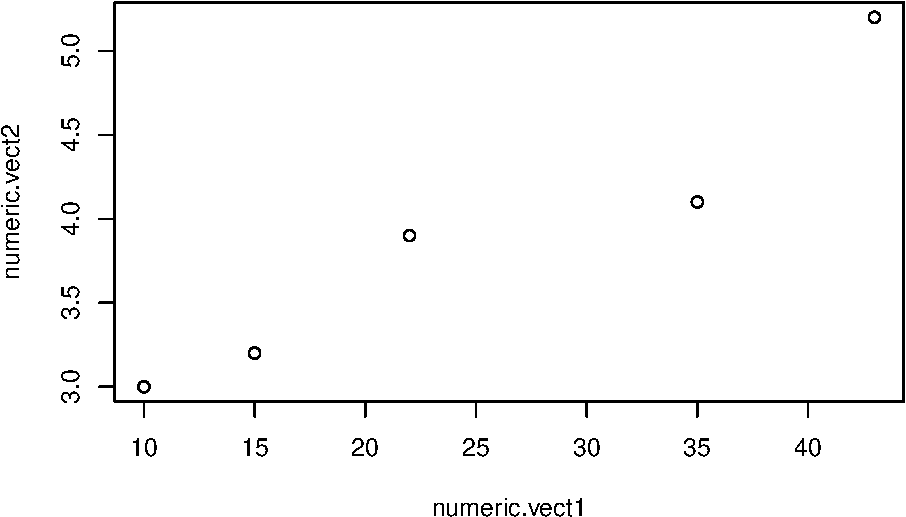
\includegraphics{lbrb_files/figure-latex/unnamed-chunk-112-1.pdf}

Note that there is a comma between the two vector names. When building plots from dataframes you usually see a tilde (\textasciitilde), but when you have two vectors you can use just a comma.

Also note the order of the vectors within the \texttt{plot()} command and which axes they appear on. The first vector is \texttt{numeric.vect1} and it appears on the horizontal x-axis.

If you want to label the axes on the plot, you can do this by giving the \texttt{plot()} function values for its optional arguments \texttt{xlab\ =} and \texttt{ylab\ =}:

\begin{Shaded}
\begin{Highlighting}[]
\FunctionTok{plot}\NormalTok{(numeric.vect1,   }\CommentTok{\# note again the comma, not a \textasciitilde{}}
\NormalTok{     numeric.vect2, }
     \AttributeTok{xlab=}\StringTok{"vector1"}\NormalTok{, }
     \AttributeTok{ylab=}\StringTok{"vector2"}\NormalTok{)}
\end{Highlighting}
\end{Shaded}

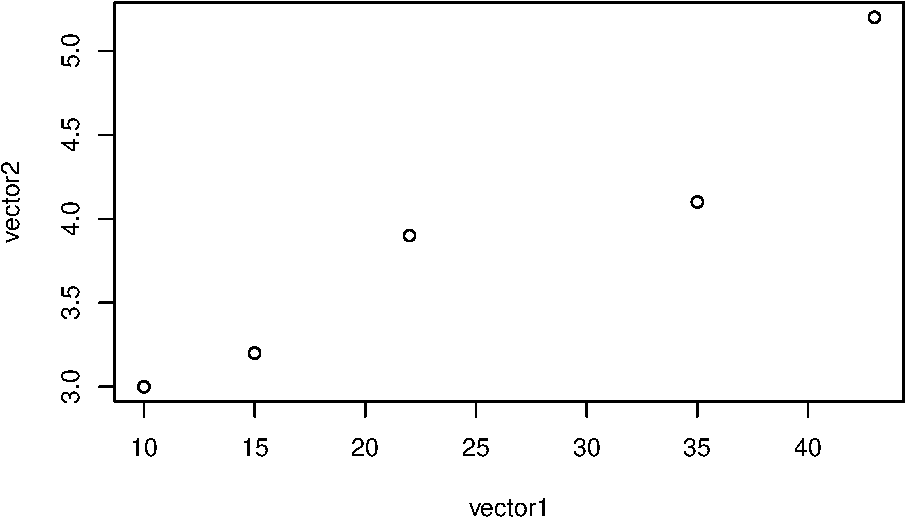
\includegraphics{lbrb_files/figure-latex/unnamed-chunk-113-1.pdf}

We can store character data in vectors so if we want we could do this to set up our labels:

\begin{Shaded}
\begin{Highlighting}[]
\NormalTok{mylabels }\OtherTok{\textless{}{-}}  \FunctionTok{c}\NormalTok{(}\StringTok{"numeric.vect1"}\NormalTok{,}\StringTok{"numeric.vect2"}\NormalTok{)}
\end{Highlighting}
\end{Shaded}

Then use bracket notation to call the labels from the vector

\begin{Shaded}
\begin{Highlighting}[]
\FunctionTok{plot}\NormalTok{(numeric.vect1, }
\NormalTok{     numeric.vect2, }
     \AttributeTok{xlab=}\NormalTok{mylabels[}\DecValTok{1}\NormalTok{],}
     \AttributeTok{ylab=}\NormalTok{mylabels[}\DecValTok{2}\NormalTok{])}
\end{Highlighting}
\end{Shaded}

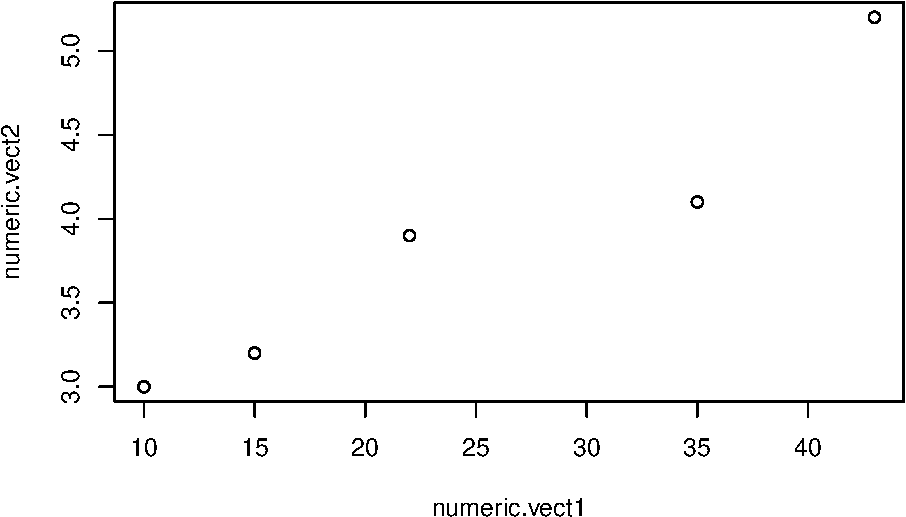
\includegraphics{lbrb_files/figure-latex/unnamed-chunk-115-1.pdf}

If we want we can use a tilde to make our plot like this:

\begin{Shaded}
\begin{Highlighting}[]
\FunctionTok{plot}\NormalTok{(numeric.vect2 }\SpecialCharTok{\textasciitilde{}}\NormalTok{ numeric.vect1)}
\end{Highlighting}
\end{Shaded}

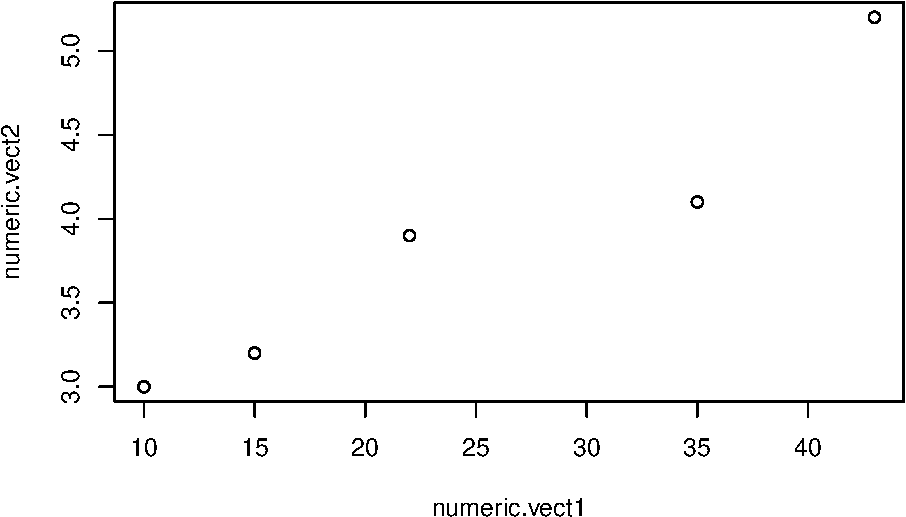
\includegraphics{lbrb_files/figure-latex/unnamed-chunk-116-1.pdf}

Note that now, \texttt{numeric.vect2} is on the left and \texttt{numeric.vect1} is on the right. This flexibility can be tricky to keep track of.

We can also combine these vectors into a dataframe and plot the data by referencing the data frame. First, we combine the two separate vectors into a dataframe using the \texttt{cbind()} command.

\begin{Shaded}
\begin{Highlighting}[]
\NormalTok{df }\OtherTok{\textless{}{-}} \FunctionTok{cbind}\NormalTok{(numeric.vect1, numeric.vect2)}
\end{Highlighting}
\end{Shaded}

Then we plot it like this, referencing the dataframe \texttt{df} via the \texttt{data\ =\ ...} argument.

\begin{Shaded}
\begin{Highlighting}[]
\FunctionTok{plot}\NormalTok{(numeric.vect2 }\SpecialCharTok{\textasciitilde{}}\NormalTok{ numeric.vect1, }\AttributeTok{data =}\NormalTok{ df)}
\end{Highlighting}
\end{Shaded}

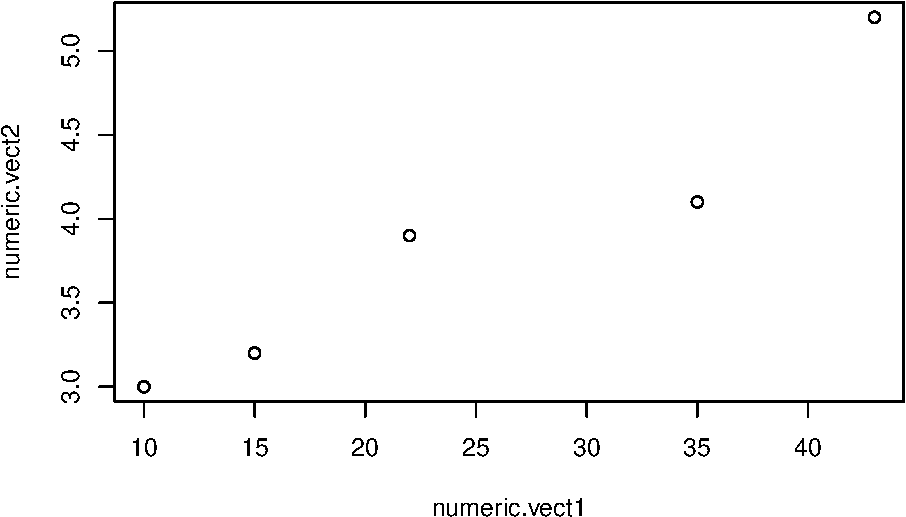
\includegraphics{lbrb_files/figure-latex/unnamed-chunk-118-1.pdf}

\hypertarget{other-plotting-packages}{%
\section{Other plotting packages}\label{other-plotting-packages}}

Base R has lots of plotting functions; additionally, people have written packages to implement new plotting capabilities. The package \texttt{ggplot2} is currently the most popular plotting package, and \texttt{ggpubr} is a package which makes \texttt{ggplot2} easier to use. For quick plots we'll use base R functions, and when we get to more important things we'll use ggplot2 and ggpubr.

\hypertarget{intro-to-r-objects}{%
\chapter{Intro to R objects}\label{intro-to-r-objects}}

\textbf{By}: Nathan Brouwer

\hypertarget{commands-used}{%
\section{Commands used}\label{commands-used}}

\begin{itemize}
\tightlist
\item
  \textless-
\item
  c()
\item
  length()
\item
  dim()
\item
  is()
\end{itemize}

\hypertarget{r-objects}{%
\section{R Objects}\label{r-objects}}

\begin{itemize}
\tightlist
\item
  Everything in R is an object, works with an object, tells you about an object, etc
\item
  We'll do a simple data analysis with a t.test and then look at properties of R objects
\item
  There are several types of objects: \textbf{vectors, matrices, lists, dataframes}
\item
  R objects can hold numbers, text, or both
\item
  A typical dataframe has columns of \textbf{numeric data} and colmns of text that represent \textbf{factor variables} (aka ``\textbf{categoical variables}'')
\end{itemize}

\hypertarget{differences-between-objects}{%
\section{Differences between objects}\label{differences-between-objects}}

Different objects are used and show up in differnt contexts.

\begin{itemize}
\tightlist
\item
  Most practical stats work in R is done with \textbf{dataframes} .\\
\item
  A dataframe is kind of like a spreadsheet, loaded into R.
\item
  For the sake of simplicity, we often load data in as a \textbf{vector}. This just makes things smoother when we are starting out.
\item
  \textbf{vectors} pop up in many places, usually in a support role until you start doing more programming.
\item
  \textbf{matrices} are occassionaly used for applied stats stuff but show up more for programming. A matrix is like a stripped-down dataframe.
\item
  \textbf{lists} show up everywhere, but you often don't know it; many R functions make lists
\item
  Understanding \textbf{lists} will help you efficiently work with stats output and make plots.
\end{itemize}

\hypertarget{the-data}{%
\section{The Data}\label{the-data}}

We'll use the following data to explore R objects.

Motulsky 2nd Ed, Chapter 30, page 220, Table 30.1. Maximal relaxaction of muscle strips of old and young rat bladders stimualted w/ high concentrations of nonrepinephrine (Frazier et al 2006). Response variable is \%E.max

\hypertarget{the-assignment-operator---makes-object}{%
\section{The assignment operator ``\textless-'' makes object}\label{the-assignment-operator---makes-object}}

The code above has made two objects. We can use several commands to learn about these objects.

\begin{itemize}
\tightlist
\item
  is(): what an object is, ie, vector, matrix, list, dataframe
\item
  length():how long an object is; only works with vectors and lists, not dataframes!
\item
  dim(): how long AND how wide and object is; doesn't work with vectors, only dataframes and matrices :(
\end{itemize}

\hypertarget{is}{%
\subsection{is()}\label{is}}

What is our ``old.E.max'' object?

\begin{Shaded}
\begin{Highlighting}[]
\FunctionTok{is}\NormalTok{(old.E.max)}
\end{Highlighting}
\end{Shaded}

\begin{verbatim}
## [1] "numeric" "vector"
\end{verbatim}

\begin{Shaded}
\begin{Highlighting}[]
\FunctionTok{is}\NormalTok{(young.E.max)}
\end{Highlighting}
\end{Shaded}

\begin{verbatim}
## [1] "numeric" "vector"
\end{verbatim}

Its a vector, containing numeric data.

What if we made a vector like this?

\begin{Shaded}
\begin{Highlighting}[]
\NormalTok{cat.variables }\OtherTok{\textless{}{-}} \FunctionTok{c}\NormalTok{(}\StringTok{"old"}\NormalTok{,}\StringTok{"old"}\NormalTok{,}\StringTok{"old"}\NormalTok{,}\StringTok{"old"}\NormalTok{,}
                   \StringTok{"old"}\NormalTok{,}\StringTok{"old"}\NormalTok{,}\StringTok{"old"}\NormalTok{,}\StringTok{"old"}\NormalTok{,}\StringTok{"old"}\NormalTok{)}
\end{Highlighting}
\end{Shaded}

And used \texttt{is()}

\begin{Shaded}
\begin{Highlighting}[]
\FunctionTok{is}\NormalTok{(cat.variables)}
\end{Highlighting}
\end{Shaded}

\begin{verbatim}
## [1] "character"           "vector"              "data.frameRowLabels"
## [4] "SuperClassMethod"
\end{verbatim}

It tells us we have a vector, containing chracter data. Not sure why it feels the need to tell us all the other stuff\ldots{}

\hypertarget{length}{%
\subsection{length()}\label{length}}

Our vector has 9 elements, or is 9 elements long.

\begin{Shaded}
\begin{Highlighting}[]
\FunctionTok{length}\NormalTok{(old.E.max)}
\end{Highlighting}
\end{Shaded}

\begin{verbatim}
## [1] 9
\end{verbatim}

Note that \texttt{dim()}, for dimension, doens't work with vectors!

\begin{Shaded}
\begin{Highlighting}[]
\FunctionTok{dim}\NormalTok{(old.E.max)}
\end{Highlighting}
\end{Shaded}

\begin{verbatim}
## NULL
\end{verbatim}

It would be nice if it said something like ``1 x 9'' for 1 row tall and 9 elements long. So it goes.

\hypertarget{str}{%
\subsection{str()}\label{str}}

\texttt{str()} stands for ``structure''.

\begin{itemize}
\tightlist
\item
  It summarizes info about an object;
\item
  I find it most useful for looking at lists.\\
\item
  If our vector here was really really long, str() would only show the first part of the vector
\end{itemize}

\begin{Shaded}
\begin{Highlighting}[]
\FunctionTok{str}\NormalTok{(old.E.max)}
\end{Highlighting}
\end{Shaded}

\begin{verbatim}
##  num [1:9] 20.8 2.8 50 33.3 29.4 38.9 29.4 52.6 14.3
\end{verbatim}

\hypertarget{c}{%
\subsection{c()}\label{c}}

\begin{itemize}
\tightlist
\item
  We typically use \texttt{c()} to gather together things like numbers, as we did to make our objects above.
\item
  note: this is \emph{lower case} ``c''!
\item
  Uppercase is something else
\item
  For me, R's font makes it hard sometiems to tell the difference between ``c'' and ``C''
\item
  If code isn't working, one problem might be a ``C'' instead of a ``c''
\end{itemize}

Use \texttt{c()} to combine two objects

\begin{Shaded}
\begin{Highlighting}[]
\NormalTok{old.plus.new }\OtherTok{\textless{}{-}} \FunctionTok{c}\NormalTok{(old.E.max, young.E.max)}
\end{Highlighting}
\end{Shaded}

Look at the legnth

\begin{Shaded}
\begin{Highlighting}[]
\FunctionTok{length}\NormalTok{(old.plus.new)}
\end{Highlighting}
\end{Shaded}

\begin{verbatim}
## [1] 17
\end{verbatim}

Note that \texttt{str()} just shows us the first few digits, not all 17

\begin{Shaded}
\begin{Highlighting}[]
\FunctionTok{str}\NormalTok{(old.plus.new)}
\end{Highlighting}
\end{Shaded}

\begin{verbatim}
##  num [1:17] 20.8 2.8 50 33.3 29.4 38.9 29.4 52.6 14.3 45.5 ...
\end{verbatim}

\hypertarget{debrief}{%
\section{Debrief}\label{debrief}}

We can\ldots{}

\begin{itemize}
\tightlist
\item
  learn about objects using length(), is(), str()
\item
  access parts of list using \$ (and also brackets)
\item
  access parts of vetors using square brackets {[} {]}
\item
  save the output of a model / test to an object
\item
  access part of lists for plotting instead of copying stuff
\end{itemize}

\hypertarget{fasta-files}{%
\chapter{FASTA Files}\label{fasta-files}}

Adapted from \href{https://en.wikipedia.org/wiki/FASTA_format}{Wikipedia}: \url{https://en.wikipedia.org/wiki/FASTA_format}

``In bioinformatics, the FASTA format is a text-based format for representing either nucleotide sequences or amino acid (protein) sequences, in which nucleotides or amino acids are represented using single-letter codes. The format allows for sequence names and comments to precede the sequences. The format originates from the FASTA alignment software, but has now become a near universal standard in the field of bioinformatics.

``The simplicity of FASTA format makes it easy to manipulate and parse sequences using text-processing tools and scripting languages like the R programming language and Python.

``The first line in a FASTA file starts with a''\textgreater'' (greater-than) symbol and holds summary information about the sequence, often starting with a unique accession number and followed by information like the name of the gene, the type of sequence, and the organism it is from.

``On the next is the sequence itself in a standard one-letter character string. Anything other than a valid character is be ignored (including spaces, tabs, asterisks, etc\ldots).

``A multiple sequence FASTA format can be obtained by concatenating several single sequence FASTA files in a common file (also known as multi-FASTA format).

``Following the header line, the actual sequence is represented. Sequences may be protein sequences or nucleic acid sequences, and they can contain gaps or alignment characters. Sequences are expected to be represented in the standard amino acid and nucleic acid codes. Lower-case letters are accepted and are mapped into upper-case; a single hyphen or dash can be used to represent a gap character; and in amino acid sequences, U and * are acceptable letters.

``FASTQ format is a form of FASTA format extended to indicate information related to sequencing. It is created by the Sanger Centre in Cambridge.

``Bioconductor.org's Biostrings package can be used to read and manipulate FASTA files in R

from \url{https://zhanglab.dcmb.med.umich.edu/FASTA/}

``FASTA format is a text-based format for representing either nucleotide sequences or peptide sequences, in which base pairs or amino acids are represented using single-letter codes. A sequence in FASTA format begins with a single-line description, followed by lines of sequence data. The description line is distinguished from the sequence data by a greater-than (''\textgreater{}``) symbol in the first column. It is recommended that all lines of text be shorter than 80 characters in length.''

\hypertarget{example-fasta-file}{%
\section{Example FASTA file}\label{example-fasta-file}}

Here is an example of the contents of a FASTA file. (If your are viewing this chapter in the form of the source .Rmd file, the \texttt{cat()} function is included just to print out the content properly and is not part of the FASTA format).

\begin{Shaded}
\begin{Highlighting}[]
\FunctionTok{cat}\NormalTok{(}\StringTok{"\textgreater{}gi|186681228|ref|YP\_001864424.1| phycoerythrobilin:ferredoxin oxidoreductase}
\StringTok{MNSERSDVTLYQPFLDYAIAYMRSRLDLEPYPIPTGFESNSAVVGKGKNQEEVVTTSYAFQTAKLRQIRA}
\StringTok{AHVQGGNSLQVLNFVIFPHLNYDLPFFGADLVTLPGGHLIALDMQPLFRDDSAYQAKYTEPILPIFHAHQ}
\StringTok{QHLSWGGDFPEEAQPFFSPAFLWTRPQETAVVETQVFAAFKDYLKAYLDFVEQAEAVTDSQNLVAIKQAQ}
\StringTok{LRYLRYRAEKDPARGMFKRFYGAEWTEEYIHGFLFDLERKLTVVK"}\NormalTok{)}
\end{Highlighting}
\end{Shaded}

\begin{verbatim}
## >gi|186681228|ref|YP_001864424.1| phycoerythrobilin:ferredoxin oxidoreductase
## MNSERSDVTLYQPFLDYAIAYMRSRLDLEPYPIPTGFESNSAVVGKGKNQEEVVTTSYAFQTAKLRQIRA
## AHVQGGNSLQVLNFVIFPHLNYDLPFFGADLVTLPGGHLIALDMQPLFRDDSAYQAKYTEPILPIFHAHQ
## QHLSWGGDFPEEAQPFFSPAFLWTRPQETAVVETQVFAAFKDYLKAYLDFVEQAEAVTDSQNLVAIKQAQ
## LRYLRYRAEKDPARGMFKRFYGAEWTEEYIHGFLFDLERKLTVVK
\end{verbatim}

\hypertarget{multiple-sequences-in-a-single-fasta-file}{%
\section{Multiple sequences in a single FASTA file}\label{multiple-sequences-in-a-single-fasta-file}}

Multiple sequences can be stored in a single FASTA file, each on separated by a line and have its own headline.

\begin{Shaded}
\begin{Highlighting}[]
\FunctionTok{cat}\NormalTok{(}\StringTok{"\textgreater{}LCBO {-} Prolactin precursor {-} Bovine}
\StringTok{MDSKGSSQKGSRLLLLLVVSNLLLCQGVVSTPVCPNGPGNCQVSLRDLFDRAVMVSHYIHDLSS}
\StringTok{EMFNEFDKRYAQGKGFITMALNSCHTSSLPTPEDKEQAQQTHHEVLMSLILGLLRSWNDPLYHL}
\StringTok{VTEVRGMKGAPDAILSRAIEIEEENKRLLEGMEMIFGQVIPGAKETEPYPVWSGLPSLQTKDED}
\StringTok{ARYSAFYNLLHCLRRDSSKIDTYLKLLNCRIIYNNNC*}

\StringTok{\textgreater{}MCHU {-} Calmodulin {-} Human, rabbit, bovine, rat, and chicken}
\StringTok{MADQLTEEQIAEFKEAFSLFDKDGDGTITTKELGTVMRSLGQNPTEAELQDMINEVDADGNGTID}
\StringTok{FPEFLTMMARKMKDTDSEEEIREAFRVFDKDGNGYISAAELRHVMTNLGEKLTDEEVDEMIREA}
\StringTok{DIDGDGQVNYEEFVQMMTAK*}

\StringTok{\textgreater{}gi|5524211|gb|AAD44166.1| cytochrome b [Elephas maximus maximus]}
\StringTok{LCLYTHIGRNIYYGSYLYSETWNTGIMLLLITMATAFMGYVLPWGQMSFWGATVITNLFSAIPYIGTNLV}
\StringTok{EWIWGGFSVDKATLNRFFAFHFILPFTMVALAGVHLTFLHETGSNNPLGLTSDSDKIPFHPYYTIKDFLG}
\StringTok{LLILILLLLLLALLSPDMLGDPDNHMPADPLNTPLHIKPEWYFLFAYAILRSVPNKLGGVLALFLSIVIL}
\StringTok{GLMPFLHTSKHRSMMLRPLSQALFWTLTMDLLTLTWIGSQPVEYPYTIIGQMASILYFSIILAFLPIAGX}
\StringTok{IENY"}\NormalTok{)}
\end{Highlighting}
\end{Shaded}

\begin{verbatim}
## >LCBO - Prolactin precursor - Bovine
## MDSKGSSQKGSRLLLLLVVSNLLLCQGVVSTPVCPNGPGNCQVSLRDLFDRAVMVSHYIHDLSS
## EMFNEFDKRYAQGKGFITMALNSCHTSSLPTPEDKEQAQQTHHEVLMSLILGLLRSWNDPLYHL
## VTEVRGMKGAPDAILSRAIEIEEENKRLLEGMEMIFGQVIPGAKETEPYPVWSGLPSLQTKDED
## ARYSAFYNLLHCLRRDSSKIDTYLKLLNCRIIYNNNC*
## 
## >MCHU - Calmodulin - Human, rabbit, bovine, rat, and chicken
## MADQLTEEQIAEFKEAFSLFDKDGDGTITTKELGTVMRSLGQNPTEAELQDMINEVDADGNGTID
## FPEFLTMMARKMKDTDSEEEIREAFRVFDKDGNGYISAAELRHVMTNLGEKLTDEEVDEMIREA
## DIDGDGQVNYEEFVQMMTAK*
## 
## >gi|5524211|gb|AAD44166.1| cytochrome b [Elephas maximus maximus]
## LCLYTHIGRNIYYGSYLYSETWNTGIMLLLITMATAFMGYVLPWGQMSFWGATVITNLFSAIPYIGTNLV
## EWIWGGFSVDKATLNRFFAFHFILPFTMVALAGVHLTFLHETGSNNPLGLTSDSDKIPFHPYYTIKDFLG
## LLILILLLLLLALLSPDMLGDPDNHMPADPLNTPLHIKPEWYFLFAYAILRSVPNKLGGVLALFLSIVIL
## GLMPFLHTSKHRSMMLRPLSQALFWTLTMDLLTLTWIGSQPVEYPYTIIGQMASILYFSIILAFLPIAGX
## IENY
\end{verbatim}

\hypertarget{multiple-sequence-alignments-can-be-stored-in-fasta-format}{%
\section{Multiple sequence alignments can be stored in FASTA format}\label{multiple-sequence-alignments-can-be-stored-in-fasta-format}}

\textbf{Aligned FASTA format} can be used to store the output of \textbf{Multiple Sequence Alignment (MSA)}. This format contains

\begin{enumerate}
\def\labelenumi{\arabic{enumi}.}
\tightlist
\item
  Multiple entries, each with their own header line
\item
  \textbf{Gaps} inserted to align sequences are indicated by \texttt{.}
\item
  Each spaces added to the beginning and end of sequences that vary in length are indicated by \texttt{\textasciitilde{}}
\end{enumerate}

In the sample FASTA file below, the \texttt{example1} sequence has a gap of 8 near its beginning. The \texttt{example2} sequence has numerous \texttt{\textasciitilde{}} indicating that this sequence is missing data from its beginning that are present in the other sequences. The \texttt{example3} sequence has numerous \texttt{\textasciitilde{}} at its end, indicating that this sequence is shorter than the others.

\begin{Shaded}
\begin{Highlighting}[]
\FunctionTok{cat}\NormalTok{(}\StringTok{"\textgreater{}example1 }
\StringTok{MKALWALLLVPLLTGCLA........EGELEVTDQLPGQSDQP.WEQALNRFWDYLRWVQ}
\StringTok{GNQARDRLEEVREQMEEVRSKMEEQTQQIRLQAEIFQARIKGWFEPLVEDMQRQWANLME}
\StringTok{KIQASVATNSIASTTVPLENQ}
\StringTok{\textgreater{}example2 }
\StringTok{\textasciitilde{}\textasciitilde{}\textasciitilde{}\textasciitilde{}\textasciitilde{}\textasciitilde{}\textasciitilde{}\textasciitilde{}\textasciitilde{}\textasciitilde{}\textasciitilde{}\textasciitilde{}\textasciitilde{}\textasciitilde{}\textasciitilde{}\textasciitilde{}\textasciitilde{}\textasciitilde{}\textasciitilde{}\textasciitilde{}\textasciitilde{}\textasciitilde{}\textasciitilde{}\textasciitilde{}\textasciitilde{}\textasciitilde{}KVQQELEPEAGWQTGQP.WEAALARFWDYLRWVQ}
\StringTok{SSRARGHLEEMREQIQEVRVKMEEQADQIRQKAEAFQARLKSWFEPLLEDMQRQWDGLVE}
\StringTok{KVQAAVAT.IPTSKPVEEP\textasciitilde{}\textasciitilde{}}
\StringTok{\textgreater{}example3 }
\StringTok{MRSLVVFFALAVLTGCQARSLFQAD..............APQPRWEEMVDRFWQYVSELN}
\StringTok{AGALKEKLEETAENL...RTSLEGRVDELTSLLAPYSQKIREQLQEVMDKIKEATAALPT}
\StringTok{QA\textasciitilde{}\textasciitilde{}\textasciitilde{}\textasciitilde{}\textasciitilde{}\textasciitilde{}\textasciitilde{}\textasciitilde{}\textasciitilde{}\textasciitilde{}\textasciitilde{}\textasciitilde{}\textasciitilde{}\textasciitilde{}\textasciitilde{}\textasciitilde{}\textasciitilde{}\textasciitilde{}\textasciitilde{}"}\NormalTok{)}
\end{Highlighting}
\end{Shaded}

\begin{verbatim}
## >example1 
## MKALWALLLVPLLTGCLA........EGELEVTDQLPGQSDQP.WEQALNRFWDYLRWVQ
## GNQARDRLEEVREQMEEVRSKMEEQTQQIRLQAEIFQARIKGWFEPLVEDMQRQWANLME
## KIQASVATNSIASTTVPLENQ
## >example2 
## ~~~~~~~~~~~~~~~~~~~~~~~~~~KVQQELEPEAGWQTGQP.WEAALARFWDYLRWVQ
## SSRARGHLEEMREQIQEVRVKMEEQADQIRQKAEAFQARLKSWFEPLLEDMQRQWDGLVE
## KVQAAVAT.IPTSKPVEEP~~
## >example3 
## MRSLVVFFALAVLTGCQARSLFQAD..............APQPRWEEMVDRFWQYVSELN
## AGALKEKLEETAENL...RTSLEGRVDELTSLLAPYSQKIREQLQEVMDKIKEATAALPT
## QA~~~~~~~~~~~~~~~~~~~
\end{verbatim}

\hypertarget{fastq-format}{%
\section{FASTQ Format}\label{fastq-format}}

Adapted from \href{https://en.wikipedia.org/wiki/FASTQ_format}{Wikipedia}: \url{https://en.wikipedia.org/wiki/FASTQ_format}

``FASTQ format is a text-based format for storing both a biological sequence (usually nucleotide sequence) and its corresponding quality scores. Both the sequence letter and quality score are each encoded with a single ASCII character for brevity.

``It was originally developed at the Wellcome Trust Sanger Institute to bundle a FASTA formatted sequence and its quality data, but has recently become the de facto standard for storing the output of high-throughput sequencing instruments such as the Illumina Genome Analyzer.

``A FASTQ file normally uses four lines per sequence.

\begin{itemize}
\tightlist
\item
  Line 1 begins with a \texttt{@} character and is followed by a sequence identifier and an optional description (like a FASTA title line).
\item
  Line 2 is the raw sequence letters.
\item
  Line 3 begins with a \texttt{+} character and is optionally followed by the same sequence identifier (and any description) again.
\item
  Line 4 encodes the \textbf{quality values} for the sequence in Line 2 of the file, and must contain the same number of symbols as letters in the sequence.
\end{itemize}

``A FASTQ file containing a single sequence might look like this:''

\begin{Shaded}
\begin{Highlighting}[]
\FunctionTok{cat}\NormalTok{(}\StringTok{"@SEQ\_ID}
\StringTok{GATTTGGGGTTCAAAGCAGTATCGATCAAATAGTAAATCCATTTGTTCAACTCACAGTTT}
\StringTok{+}
\StringTok{!\textquotesingle{}\textquotesingle{}*((((***+))\%\%\%++)(\%\%\%\%).1***{-}+*\textquotesingle{}\textquotesingle{}))**55CCF\textgreater{}\textgreater{}\textgreater{}\textgreater{}\textgreater{}\textgreater{}CCCCCCC65"}\NormalTok{)}
\end{Highlighting}
\end{Shaded}

\begin{verbatim}
## @SEQ_ID
## GATTTGGGGTTCAAAGCAGTATCGATCAAATAGTAAATCCATTTGTTCAACTCACAGTTT
## +
## !''*((((***+))%%%++)(%%%%).1***-+*''))**55CCF>>>>>>CCCCCCC65
\end{verbatim}

``Here are the quality value characters in left-to-right increasing order of quality (ASCII):''

\begin{Shaded}
\begin{Highlighting}[]
 \SpecialCharTok{!}\StringTok{"\#$\%\&\textquotesingle{}()*+,{-}./0123456789:;\textless{}=\textgreater{}?@ABCDEFGHIJKLMNOPQRSTUVWXYZ[\textbackslash{}]\^{}\_\textasciigrave{}abcdefghijklmnopqrstuvwxyz\{|\}\textasciitilde{}}
\end{Highlighting}
\end{Shaded}

FASTQ files typically do not include line breaks and do not wrap around when they reach the width of a normal page or file.

\hypertarget{downloading-dna-sequences-as-fasta-files-in-r}{%
\chapter{Downloading DNA sequences as FASTA files in R}\label{downloading-dna-sequences-as-fasta-files-in-r}}

This is a modification of \href{https://a-little-book-of-r-for-bioinformatics.readthedocs.io/en/latest/src/chapter1.html}{``DNA Sequence Statistics''} from Avril Coghlan's \href{https://a-little-book-of-r-for-bioinformatics.readthedocs.io/en/latest/index.html}{\emph{A little book of R for bioinformatics.}}. Most of the text and code was originally written by Dr.~Coghlan and distributed under the \href{https://creativecommons.org/licenses/by/3.0/us/}{Creative Commons 3.0} license.

\textbf{NOTE}: There is some reduncnacy in this current draft that needs to be eliminated.

\hypertarget{functions-1}{%
\subsection{Functions}\label{functions-1}}

\begin{itemize}
\tightlist
\item
  library()
\item
  help()
\item
  length
\item
  table
\item
  seqinr::GC()
\item
  seqinr::count()
\item
  seqinr::write.fasta()
\end{itemize}

\hypertarget{softwarewebsites}{%
\subsection{Software/websites}\label{softwarewebsites}}

\begin{itemize}
\tightlist
\item
  www.ncbi.nlm.nih.gov
\item
  Text editors (e.g.~Notepad++, TextWrangler)
\end{itemize}

\hypertarget{r-vocabulary}{%
\subsection{R vocabulary}\label{r-vocabulary}}

\begin{itemize}
\tightlist
\item
  list
\item
  library
\item
  package
\item
  CRAN
\item
  wrapper
\end{itemize}

\hypertarget{file-types}{%
\subsection{File types}\label{file-types}}

\begin{itemize}
\tightlist
\item
  FASTA
\end{itemize}

\hypertarget{bioinformatics-vocabulary}{%
\subsection{Bioinformatics vocabulary}\label{bioinformatics-vocabulary}}

\begin{itemize}
\tightlist
\item
  accession, accession number
\item
  NCBI
\item
  NCBI Sequence Database
\item
  EMBL Sequence Database
\item
  FASTA file
\end{itemize}

\hypertarget{organisms-and-sequence-accessions}{%
\subsection{Organisms and Sequence accessions}\label{organisms-and-sequence-accessions}}

\begin{itemize}
\tightlist
\item
  Dengue virus: DEN-1, DEN-2, DEN-3, and DEN-4.
\end{itemize}

The NCBI accessions for the DNA sequences of the DEN-1, DEN-2, DEN-3, and DEN-4 Dengue viruses are NC\_001477, NC\_001474, NC\_001475 and NC\_002640, respectively.

According to Wikipedia

\begin{quote}
``Dengue virus (DENV) is the cause of dengue fever. It is a mosquito-borne, single positive-stranded RNA virus \ldots{} Five serotypes of the virus have been found, all of which can cause the full spectrum of disease. Nevertheless, scientists' understanding of dengue virus may be simplistic, as rather than distinct \ldots{} groups, a continuum appears to exist.'' \url{https://en.wikipedia.org/wiki/Dengue_virus}
\end{quote}

\hypertarget{preliminaries}{%
\subsection{Preliminaries}\label{preliminaries}}

\begin{Shaded}
\begin{Highlighting}[]
\FunctionTok{library}\NormalTok{(rentrez)}
\FunctionTok{library}\NormalTok{(compbio4all) }
\end{Highlighting}
\end{Shaded}

\hypertarget{dna-sequence-statistics-part-1}{%
\section{DNA Sequence Statistics: Part 1}\label{dna-sequence-statistics-part-1}}

\hypertarget{using-r-for-bioinformatics}{%
\subsection{Using R for Bioinformatics}\label{using-r-for-bioinformatics}}

The chapter will guide you through the process of using R to carry out simple analyses that are common in bioinformatics and computational biology. In particular, the focus is on computational analysis of biological sequence data such as genome sequences and protein sequences. The programming approaches, however, are broadly generalizable to statistics and data science.

The tutorials assume that the reader has some basic knowledge of biology, but not necessarily of bioinformatics. The focus is to explain simple bioinformatics analysis, and to explain how to carry out these analyses using \emph{R}.

\hypertarget{r-packages-for-bioinformatics-bioconductor-and-seqinr}{%
\subsection{R packages for bioinformatics: Bioconductor and SeqinR}\label{r-packages-for-bioinformatics-bioconductor-and-seqinr}}

Many authors have written \emph{R} packages for performing a wide variety of analyses. These do not come with the standard \emph{R} installation, but must be installed and loaded as ``add-ons''.

Bioinformaticians have written numerous specialized packages for \emph{R}. In this tutorial, you will learn to use some of the function in the \href{https://cran.r-project.org/web/packages/seqinr/index.html}{\texttt{SeqinR}} package to to carry out simple analyses of DNA sequences. (\texttt{SeqinR} can retrieve sequences from a DNA sequence database, but this has largely been replaced by the functions in the package \texttt{rentrez})

Many well-known bioinformatics packages for \emph{R} are in the Bioconductor set of \emph{R} packages (www.bioconductor.org), which contains packages with many \emph{R} functions for analyzing biological data sets such as microarray data. The \href{https://cran.r-project.org/web/packages/seqinr/index.html}{\texttt{SeqinR}} package is from CRAN, which contains R functions for obtaining sequences from DNA and protein sequence databases, and for analyzing DNA and protein sequences.

We will also use functions from the \texttt{rentrez} and \texttt{ape} packages.

Remember that you can ask for more information about a particular \emph{R} command by using the \texttt{help()} function. For example, to ask for more information about the \texttt{library()}, you can type:

\begin{Shaded}
\begin{Highlighting}[]
\FunctionTok{help}\NormalTok{(}\StringTok{"library"}\NormalTok{)}
\end{Highlighting}
\end{Shaded}

You can also do this

\begin{Shaded}
\begin{Highlighting}[]
\NormalTok{?library}
\end{Highlighting}
\end{Shaded}

\hypertarget{fasta-file-format}{%
\subsection{FASTA file format}\label{fasta-file-format}}

The FASTA format is a simple and widely used format for storing biological (e.g.~DNA or protein) sequences. It was first used by the \href{https://en.wikipedia.org/wiki/FASTA}{FASTA program} for sequence alignment in the 1980s and has been adopted as standard by many other programs.

FASTA files begin with a single-line description starting with a greater-than sign \texttt{\textgreater{}} character, followed on the next line by the sequences. Here is an example of a FASTA file. (If you're looking at the source script for this lesson you'll see the \texttt{cat()} command, which is just a text display function used format the text when you run the code).

\begin{verbatim}
## >A06852 183 residues MPRLFSYLLGVWLLLSQLPREIPGQSTNDFIKACGRELVRLWVEICGSVSWGRTALSLEEPQLETGPPAETMPSSITKDAEILKMMLEFVPNLPQELKATLSERQPSLRELQQSASKDSNLNFEEFKKIILNRQNEAEDKSLLELKNLGLDKHSRKKRLFRMTLSEKCCQVGCIRKDIARLC
\end{verbatim}

\hypertarget{the-ncbi-sequence-database}{%
\subsection{The NCBI sequence database}\label{the-ncbi-sequence-database}}

The US \href{www.ncbi.nlm.nih.gov}{National Centre for Biotechnology Information (NCBI)} maintains the \textbf{NCBI Sequence Database}, a huge database of all the DNA and protein sequence data that has been collected. There are also similar databases in Europe, the \href{www.ebi.ac.uk/embl}{European Molecular Biology Laboratory (EMBL) Sequence Database}, and Japan, the \href{www.ddbj.nig.ac.jp}{DNA Data Bank of Japan (DDBJ)}. These three databases exchange data every night, so at any one point in time, they contain almost identical data.

Each sequence in the NCBI Sequence Database is stored in a separate \textbf{record}, and is assigned a unique identifier that can be used to refer to that record. The identifier is known as an \textbf{accession}, and consists of a mixture of numbers and letters.

For example, Dengue virus causes Dengue fever, which is classified as a \textbf{neglected tropical disease} by the World Health Organization (WHO), is classified by any one of four types of Dengue virus: DEN-1, DEN-2, DEN-3, and DEN-4. The NCBI accessions for the DNA sequences of the DEN-1, DEN-2, DEN-3, and DEN-4 Dengue viruses are

\begin{itemize}
\tightlist
\item
  NC\_001477
\item
  NC\_001474
\item
  NC\_001475\\
\item
  NC\_002640
\end{itemize}

Note that because the NCBI Sequence Database, the EMBL Sequence Database, and DDBJ exchange data every night, the DEN-1 (and DEN-2, DEN-3, DEN-4) Dengue virus sequence are present in all three databases, but they have different accessions in each database, as they each use their own numbering systems for referring to their own sequence records.

\hypertarget{retrieving-genome-sequence-data-using-rentrez}{%
\subsection{Retrieving genome sequence data using rentrez}\label{retrieving-genome-sequence-data-using-rentrez}}

You can retrieve sequence data from NCBI directly from \emph{R} using the \texttt{rentrez} package. The DEN-1 Dengue virus genome sequence has NCBI accession NC\_001477. To retrieve a sequence with a particular NCBI accession, you can use the function \texttt{entrez\_fetch()} from the \texttt{rentrez} package. Note that to be specific where the function comes from I write it as \texttt{package::function()}.

\begin{Shaded}
\begin{Highlighting}[]
\NormalTok{dengueseq\_fasta }\OtherTok{\textless{}{-}}\NormalTok{ rentrez}\SpecialCharTok{::}\FunctionTok{entrez\_fetch}\NormalTok{(}\AttributeTok{db =} \StringTok{"nucleotide"}\NormalTok{, }
                          \AttributeTok{id =} \StringTok{"NC\_001477"}\NormalTok{, }
                          \AttributeTok{rettype =} \StringTok{"fasta"}\NormalTok{)}
\end{Highlighting}
\end{Shaded}

Note that the ``\emph{'' in the name is just an arbitrary way to separate two words. Another common format would be \texttt{dengueseq.fasta}. Some people like \texttt{dengueseqFasta}, called \textbf{camel case} because the capital letter makes a hump in the middle of the word. Underscores are becoming most common and are favored by developers associated with RStudio and the \textbf{tidyverse} of packages that many data scientists use. I switch between ''.'' and ''}'' as separators, usually favoring ``\_'' for function names and ``.'' for objects; I personally find camel case harder to read and to type.

Ok, so what exactly have we done when we made \texttt{dengueseq\_fasta}? We have an R object \texttt{dengueseq\_fasta} which has the sequence linked to the accession number ``NC\_001477.'' So where is the sequence, and what is it?

First, what is it?

\begin{Shaded}
\begin{Highlighting}[]
\FunctionTok{is}\NormalTok{(dengueseq\_fasta)}
\end{Highlighting}
\end{Shaded}

\begin{verbatim}
## [1] "character"           "vector"              "data.frameRowLabels"
## [4] "SuperClassMethod"
\end{verbatim}

\begin{Shaded}
\begin{Highlighting}[]
\FunctionTok{class}\NormalTok{(dengueseq\_fasta)}
\end{Highlighting}
\end{Shaded}

\begin{verbatim}
## [1] "character"
\end{verbatim}

How big is it? Try the \texttt{dim()} and \texttt{length()} commands and see which one works. Do you know why one works and the other doesn't?

\begin{Shaded}
\begin{Highlighting}[]
\FunctionTok{dim}\NormalTok{(dengueseq\_fasta)}
\end{Highlighting}
\end{Shaded}

\begin{verbatim}
## NULL
\end{verbatim}

\begin{Shaded}
\begin{Highlighting}[]
\FunctionTok{length}\NormalTok{(dengueseq\_fasta)}
\end{Highlighting}
\end{Shaded}

\begin{verbatim}
## [1] 1
\end{verbatim}

The size of the object is 1. Why is this? This is the genomics sequence of a virus, so you'd expect it to be fairly large. We'll use another function below to explore that issue. Think about this first: how many pieces of unique information are in the \texttt{dengueseq} object? In what sense is there only \emph{one} piece of information?

If we want to actually see the sequence we can type just type \texttt{dengueseq\_fasta} and press enter. This will print the WHOLE genomic sequence out but it will probably run of your screen.

\begin{Shaded}
\begin{Highlighting}[]
\NormalTok{dengueseq\_fasta}
\end{Highlighting}
\end{Shaded}

This is a whole genome sequence, but its stored as single entry in a vector, so the \texttt{length()} command just tells us how many entries there are in the vector, which is just one! What this means is that the entire genomic sequence is stored in a single entry of the vector \texttt{dengueseq\_fasta}. (If you're not following along with this, no worries - its not essential to actually working with the data)

If we want to actually know how long the sequence is, we need to use the function \texttt{nchar()}.

\begin{Shaded}
\begin{Highlighting}[]
\FunctionTok{nchar}\NormalTok{(dengueseq\_fasta)}
\end{Highlighting}
\end{Shaded}

\begin{verbatim}
## [1] 10935
\end{verbatim}

The sequence is 10935 bases long. All of these bases are stored as a single \textbf{character string} with no spaces in a single entry of our \texttt{dengueseq\_fasta} vector. This isn't actually a useful format for us, so below were' going to convert it to something more useful.

If we want to see just part of the sequence we can use the \texttt{strtrim()} function. Before you run the code below, predict what the 100 means.

\begin{Shaded}
\begin{Highlighting}[]
\FunctionTok{strtrim}\NormalTok{(dengueseq\_fasta, }\DecValTok{100}\NormalTok{)}
\end{Highlighting}
\end{Shaded}

\begin{verbatim}
## [1] ">NC_001477.1 Dengue virus 1, complete genome\nAGTTGTTAGTCTACGTGGACCGACAAGAACAGTTTCGAATCGGAAGCTTGCTTAAC"
\end{verbatim}

Note that at the end of the name is a slash followed by an n, which indicates to the computer that this is a \textbf{newline}; this is read by text editor, but is ignored by R in this context.

\begin{Shaded}
\begin{Highlighting}[]
\FunctionTok{strtrim}\NormalTok{(dengueseq\_fasta, }\DecValTok{45}\NormalTok{)}
\end{Highlighting}
\end{Shaded}

\begin{verbatim}
## [1] ">NC_001477.1 Dengue virus 1, complete genome\nA"
\end{verbatim}

After the \texttt{\textbackslash{}\textbackslash{}n} begins the sequence, which will continue on for a LOOOOOONG way. Let's just print a little bit.

\begin{Shaded}
\begin{Highlighting}[]
\FunctionTok{strtrim}\NormalTok{(dengueseq\_fasta, }\DecValTok{52}\NormalTok{)}
\end{Highlighting}
\end{Shaded}

\begin{verbatim}
## [1] ">NC_001477.1 Dengue virus 1, complete genome\nAGTTGTTA"
\end{verbatim}

Let's print some more. Do you notice anything beside A, T, C and G in the sequence?

\begin{Shaded}
\begin{Highlighting}[]
\FunctionTok{strtrim}\NormalTok{(dengueseq\_fasta, }\DecValTok{200}\NormalTok{)}
\end{Highlighting}
\end{Shaded}

\begin{verbatim}
## [1] ">NC_001477.1 Dengue virus 1, complete genome\nAGTTGTTAGTCTACGTGGACCGACAAGAACAGTTTCGAATCGGAAGCTTGCTTAACGTAGTTCTAACAGT\nTTTTTATTAGAGAGCAGATCTCTGATGAACAACCAACGGAAAAAGACGGGTCGACCGTCTTTCAATATGC\nTGAAACGCGCGAGAAA"
\end{verbatim}

Again, there are the \texttt{\textbackslash{}\textbackslash{}n} newline characters, which tell text editors and wordprocessors how to display the file.

Now that we a sense of what we're looking at let's explore the \texttt{dengueseq\_fasta} a bit more.

We can find out more information about what it is using the \texttt{class()}command.

\begin{Shaded}
\begin{Highlighting}[]
\FunctionTok{class}\NormalTok{(dengueseq\_fasta)}
\end{Highlighting}
\end{Shaded}

\begin{verbatim}
## [1] "character"
\end{verbatim}

As noted before, this is character data.

Many things in R are vectors so we can ask \emph{R }\texttt{is.vector()}

\begin{Shaded}
\begin{Highlighting}[]
\FunctionTok{is.vector}\NormalTok{(dengueseq\_fasta)}
\end{Highlighting}
\end{Shaded}

\begin{verbatim}
## [1] TRUE
\end{verbatim}

Yup, that's true.

Ok, let's see what else. A handy though often verbose command is \texttt{is()}, which tells us what an object, well, what it is:

\begin{Shaded}
\begin{Highlighting}[]
\FunctionTok{is}\NormalTok{(dengueseq\_fasta)}
\end{Highlighting}
\end{Shaded}

\begin{verbatim}
## [1] "character"           "vector"              "data.frameRowLabels"
## [4] "SuperClassMethod"
\end{verbatim}

There is a lot here but if you scan for some key words you will see ``character'' and ``vector'' at the top. The other stuff you can ignore. The first two things, though, tell us the dengueseq\_fasta is a \textbf{vector} of the class \textbf{character}: that is, a \textbf{character vector}.

Another handy function is \texttt{str()}, which gives us a peak at the context and structure of an \emph{R} object. This is most useful when you are working in the R console or with dataframes, but is a useful function to run on all \emph{R} objects. How does this output differ from other ways we've displayed dengueseq\_fasta?

\begin{Shaded}
\begin{Highlighting}[]
\FunctionTok{str}\NormalTok{(dengueseq\_fasta)}
\end{Highlighting}
\end{Shaded}

\begin{verbatim}
##  chr ">NC_001477.1 Dengue virus 1, complete genome\nAGTTGTTAGTCTACGTGGACCGACAAGAACAGTTTCGAATCGGAAGCTTGCTTAACGTAGTTCTA"| __truncated__
\end{verbatim}

We know it contains character data - how many characters? \texttt{nchar()} for ``number of characters'' answers that:

\begin{Shaded}
\begin{Highlighting}[]
\FunctionTok{nchar}\NormalTok{(dengueseq\_fasta)}
\end{Highlighting}
\end{Shaded}

\begin{verbatim}
## [1] 10935
\end{verbatim}

\hypertarget{optional-saving-fasta-files}{%
\section{OPTIONAL: Saving FASTA files}\label{optional-saving-fasta-files}}

We can save our data as .fasta file for safe keeping. The \texttt{write()} function will save the data we downloaded as a plain text file.

\begin{Shaded}
\begin{Highlighting}[]
\FunctionTok{write}\NormalTok{(dengueseq\_fasta, }
      \AttributeTok{file=}\StringTok{"dengueseq.fasta"}\NormalTok{)}
\end{Highlighting}
\end{Shaded}

If you do this, you'll need to figure out where \emph{R} is saving things, which requires and understanding \emph{R's} \textbf{file system}, which can take some getting used to, especially if you're new to programming. As a start, you can see where \emph{R} saves things by using the \texttt{getwd()} command, which tells you where on your harddrive R currently is using as its home base for files.

\begin{Shaded}
\begin{Highlighting}[]
\FunctionTok{getwd}\NormalTok{()}
\end{Highlighting}
\end{Shaded}

\begin{verbatim}
## [1] "/Users/nlb24/google_backup_sync_nlb24/lbrb"
\end{verbatim}

\hypertarget{next-steps}{%
\section{Next steps}\label{next-steps}}

On their own, FASTA files in R are not directly useful. In the next lesson we'll process our \texttt{dengueseq\_fasta} file so that we can use it in analyses.

\hypertarget{downloading-dna-sequences-as-fasta-files-in-r-1}{%
\chapter{Downloading DNA sequences as FASTA files in R}\label{downloading-dna-sequences-as-fasta-files-in-r-1}}

This is a modification of \href{https://a-little-book-of-r-for-bioinformatics.readthedocs.io/en/latest/src/chapter1.html}{``DNA Sequence Statistics''} from Avril Coghlan's \href{https://a-little-book-of-r-for-bioinformatics.readthedocs.io/en/latest/index.html}{\emph{A little book of R for bioinformatics.}}. Most of the text and code was originally written by Dr.~Coghlan and distributed under the \href{https://creativecommons.org/licenses/by/3.0/us/}{Creative Commons 3.0} license.

\hypertarget{preliminaries-1}{%
\section{Preliminaries}\label{preliminaries-1}}

We'll need the \texttt{dengueseq\_fasta} FASTA data object, which is in the \texttt{compbio4all} package. We'll also use the \texttt{stringr} package for cleaning up the FASTA data, which can be downloaded with \texttt{install.packages("stringr")}

\begin{Shaded}
\begin{Highlighting}[]
\CommentTok{\# compbio4all, which has dengueseq\_fasta}
\FunctionTok{library}\NormalTok{(compbio4all)}
\FunctionTok{data}\NormalTok{(dengueseq\_fasta)}

\CommentTok{\# stringr, for data cleaning}
\FunctionTok{library}\NormalTok{(stringr)}
\end{Highlighting}
\end{Shaded}

\hypertarget{convert-fasta-sequence-to-an-r-variable}{%
\section{Convert FASTA sequence to an R variable}\label{convert-fasta-sequence-to-an-r-variable}}

We can't actually do much with the contents of the \texttt{dengueseq\_fasta} we downloaded with the \texttt{rentrez} package except read them. If we want do address some biological questions with the data we need is to convert it into a data structure \emph{R} can work with.

There are several things we need to remove:

\begin{enumerate}
\def\labelenumi{\arabic{enumi}.}
\tightlist
\item
  The \textbf{meta data} line \texttt{\textgreater{}NC\_001477.1\ Dengue\ virus\ 1,\ complete\ genome} (metadata is ``data'' about data, such as where it came from, what it is, who made it, etc.).
\item
  All the \texttt{\textbackslash{}n} that show up in the file (these are the \textbf{line breaks}).
\item
  Put each nucleotide of the sequence into its own spot in a vector.
\end{enumerate}

There are functions that can do this automatically, but

\begin{enumerate}
\def\labelenumi{\arabic{enumi}.}
\tightlist
\item
  I haven't found one I like, and
\item
  walking through this will help you understand the types of operations you can do on text data.
\end{enumerate}

The first two steps involve removing things from the existing \textbf{character string} that contains the sequence. The third step will split the single continuous character string like ``AGTTGTTAGTCTACGT\ldots{}'' into a \textbf{character vector} like \texttt{c("A","G","T","T","G","T","T","A","G","T","C","T","A","C","G","T"...)}, where each element of the vector is a single character a stored in a separate slot in the vector.

\hypertarget{removing-unwanted-characters}{%
\subsection{Removing unwanted characters}\label{removing-unwanted-characters}}

The second item is the easiest to take care of. \emph{R} and many programming languages have tools called \textbf{regular expressions} that allow you to manipulate text. R has a function called \texttt{gsub()} which allows you to substitute or delete character data from a string. First I'll remove all those \texttt{\textbackslash{}n} values.

The regular expression function \texttt{gsub()} takes three arguments:
1. \texttt{pattern\ =\ ...}. This is what we need it to find so we can replace it.
1. \texttt{replacement\ =\ ...}. The replacement.
1. \texttt{x\ =\ ...}. A character string or vector where \texttt{gsub()} will do its work.

We need to get rid of the \texttt{\textbackslash{}n} so that we are left with only A, T and G, which are the actually information of the sequence. We want \texttt{\textbackslash{}n} completely removed, so the replacement will be \texttt{""}, which is as set of quotation marks with nothing in the middle, which means ``delete the target pattern and put nothing in its place.''

One thing that is tricky about regular expressions is that many characters have special meaning to the functions, such as slashes, dollar signs, and brackets. So, if you want to find and replace one of these specially designated characters you need to put a slash in front of them. So when we set the pattern, instead of setting the pattern to a slash before an n \texttt{\textbackslash{}n}, we have to give it two slashes \texttt{\textbackslash{}\textbackslash{}n}.

Here is the regular expression to delete the newline character \textbackslash n.

\begin{Shaded}
\begin{Highlighting}[]
 \CommentTok{\# note: we want to find all the \textbackslash{}n, but need to set the pattern as \textbackslash{}\textbackslash{}n}
\NormalTok{dengueseq\_vector }\OtherTok{\textless{}{-}} \FunctionTok{gsub}\NormalTok{(}\AttributeTok{pattern =} \StringTok{"}\SpecialCharTok{\textbackslash{}\textbackslash{}}\StringTok{n"}\NormalTok{,  }
                         \AttributeTok{replacement =} \StringTok{""}\NormalTok{, }
                         \AttributeTok{x =}\NormalTok{ dengueseq\_fasta)}
\end{Highlighting}
\end{Shaded}

We can use \texttt{strtrim()} to see if it worked

\begin{Shaded}
\begin{Highlighting}[]
\FunctionTok{strtrim}\NormalTok{(dengueseq\_vector, }\DecValTok{80}\NormalTok{)}
\end{Highlighting}
\end{Shaded}

\begin{verbatim}
## [1] ">NC_001477.1 Dengue virus 1, complete genomeAGTTGTTAGTCTACGTGGACCGACAAGAACAGTTTC"
\end{verbatim}

Now for the metadata header. This is a bit complex, but the following code is going to take all the that occurs before the beginning of the sequence (``AGTTGTTAGTC'') and delete it.

First, I'll define what I want to get rid of in an \emph{R} object. This will make the \textbf{call} to \texttt{gsub()} a little cleaner to read

\begin{Shaded}
\begin{Highlighting}[]
\NormalTok{seq.header }\OtherTok{\textless{}{-}} \StringTok{"\textgreater{}NC\_001477.1 Dengue virus 1, complete genome"}
\end{Highlighting}
\end{Shaded}

Now I'll get rid of the header with with \texttt{gsub()}.

\begin{Shaded}
\begin{Highlighting}[]
\NormalTok{dengueseq\_vector }\OtherTok{\textless{}{-}} \FunctionTok{gsub}\NormalTok{(}\AttributeTok{pattern =}\NormalTok{ seq.header, }\CommentTok{\# object defined above}
                         \AttributeTok{replacement =} \StringTok{""}\NormalTok{, }
                         \AttributeTok{x =}\NormalTok{ dengueseq\_vector)}
\end{Highlighting}
\end{Shaded}

See if it worked:

\begin{Shaded}
\begin{Highlighting}[]
\FunctionTok{strtrim}\NormalTok{(dengueseq\_vector, }\DecValTok{80}\NormalTok{)}
\end{Highlighting}
\end{Shaded}

\begin{verbatim}
## [1] "AGTTGTTAGTCTACGTGGACCGACAAGAACAGTTTCGAATCGGAAGCTTGCTTAACGTAGTTCTAACAGTTTTTTATTAG"
\end{verbatim}

\hypertarget{spliting-unbroken-strings-in-character-vectors}{%
\subsection{Spliting unbroken strings in character vectors}\label{spliting-unbroken-strings-in-character-vectors}}

Now the more complex part. We need to split up a continuous, unbroken string of letters into a vector where each letter is on its own. This can be done with the \texttt{str\_split()} function (``string split'') from the \texttt{stringr} package. The notation \texttt{stringr::str\_split()} mean ``use the \texttt{str\_split} function from from the \texttt{stringr} package.'' More specifically, it temporarily loads the \texttt{stringr} package and gives R access to just the \texttt{str\_split} function. These allows you to call a single function without loading the whole library.

There are several arguments to \texttt{str\_split}, and I've tacked a \texttt{{[}{[}1{]}{]}} on to the end.

First, run the command

\begin{Shaded}
\begin{Highlighting}[]
\NormalTok{dengueseq\_vector\_split }\OtherTok{\textless{}{-}}\NormalTok{ stringr}\SpecialCharTok{::}\FunctionTok{str\_split}\NormalTok{(dengueseq\_vector,}
                                       \AttributeTok{pattern =} \StringTok{""}\NormalTok{,}
                                       \AttributeTok{simplify =} \ConstantTok{FALSE}\NormalTok{)[[}\DecValTok{1}\NormalTok{]]}
\end{Highlighting}
\end{Shaded}

Look at the output with str()

\begin{Shaded}
\begin{Highlighting}[]
\FunctionTok{str}\NormalTok{(dengueseq\_vector\_split)}
\end{Highlighting}
\end{Shaded}

\begin{verbatim}
##  chr [1:10735] "A" "G" "T" "T" "G" "T" "T" "A" "G" "T" "C" "T" "A" "C" "G" ...
\end{verbatim}

We can explore what the different arguments do by modifying them. Change \texttt{pattern\ =\ ""\ to\ pattern\ =\ "A"}. Can you figure out what happened?

\begin{Shaded}
\begin{Highlighting}[]
\CommentTok{\# re{-}run the command with "pattern  = "A"}
\NormalTok{dengueseq\_vector\_split2 }\OtherTok{\textless{}{-}}\NormalTok{ stringr}\SpecialCharTok{::}\FunctionTok{str\_split}\NormalTok{(dengueseq\_vector,}
                                       \AttributeTok{pattern =} \StringTok{"A"}\NormalTok{,}
                                       \AttributeTok{simplify =} \ConstantTok{FALSE}\NormalTok{)[[}\DecValTok{1}\NormalTok{]]}
\FunctionTok{str}\NormalTok{(dengueseq\_vector\_split2)}
\end{Highlighting}
\end{Shaded}

\begin{verbatim}
##  chr [1:3427] "" "GTTGTT" "GTCT" "CGTGG" "CCG" "C" "" "G" "" "C" "GTTTCG" ...
\end{verbatim}

And try it with \texttt{pattern\ =\ ""\ to\ pattern\ =\ "G"}.

\begin{Shaded}
\begin{Highlighting}[]
\CommentTok{\# re{-}run the command with "pattern  = "G"}
\NormalTok{dengueseq\_vector\_split3 }\OtherTok{\textless{}{-}}\NormalTok{ stringr}\SpecialCharTok{::}\FunctionTok{str\_split}\NormalTok{(dengueseq\_vector,}
                                       \AttributeTok{pattern =} \StringTok{"G"}\NormalTok{,}
                                       \AttributeTok{simplify =} \ConstantTok{FALSE}\NormalTok{)[[}\DecValTok{1}\NormalTok{]]}
\FunctionTok{str}\NormalTok{(dengueseq\_vector\_split3)}
\end{Highlighting}
\end{Shaded}

\begin{verbatim}
##  chr [1:2771] "A" "TT" "TTA" "TCTAC" "T" "" "ACC" "ACAA" "AACA" "TTTC" ...
\end{verbatim}

Run this code to compare the two ways we just used \texttt{str\_split} (don't worry what it does). Does this help you see what's up?

\begin{Shaded}
\begin{Highlighting}[]
\FunctionTok{options}\NormalTok{(}\AttributeTok{str =} \FunctionTok{strOptions}\NormalTok{(}\AttributeTok{vec.len =} \DecValTok{10}\NormalTok{))}
\FunctionTok{str}\NormalTok{(}\FunctionTok{list}\NormalTok{(dengueseq\_vector\_split[}\DecValTok{1}\SpecialCharTok{:}\DecValTok{20}\NormalTok{],}
\NormalTok{     dengueseq\_vector\_split2[}\DecValTok{1}\SpecialCharTok{:}\DecValTok{10}\NormalTok{], }
\NormalTok{     dengueseq\_vector\_split3[}\DecValTok{1}\SpecialCharTok{:}\DecValTok{10}\NormalTok{]))}
\end{Highlighting}
\end{Shaded}

\begin{verbatim}
## List of 3
##  $ : chr [1:20] "A" "G" "T" "T" "G" "T" "T" "A" "G" "T" ...
##  $ : chr [1:10] "" "GTTGTT" "GTCT" "CGTGG" "CCG" "C" "" "G" "" "C"
##  $ : chr [1:10] "A" "TT" "TTA" "TCTAC" "T" "" "ACC" "ACAA" "AACA" "TTTC"
\end{verbatim}

So, what does the \texttt{pattern\ =\ ...} argument do? For more info open up the help file for \texttt{str\_split} by calling \texttt{?str\_split}.

Something cool which we will explore in the next exercise is that we can do summaries on vectors of nucleotides, like this:

\begin{Shaded}
\begin{Highlighting}[]
\FunctionTok{table}\NormalTok{(dengueseq\_vector\_split)}
\end{Highlighting}
\end{Shaded}

\begin{verbatim}
## dengueseq_vector_split
##    A    C    G    T 
## 3426 2240 2770 2299
\end{verbatim}

\hypertarget{dna-descriptive-statics---part-1}{%
\chapter{DNA descriptive statics - Part 1}\label{dna-descriptive-statics---part-1}}

\textbf{By}: Avril Coghlan

\textbf{Adapted, edited and expanded}: Nathan Brouwer (\href{mailto:brouwern@gmail.com}{\nolinkurl{brouwern@gmail.com}}) under the Creative Commons 3.0 Attribution License \href{https://creativecommons.org/licenses/by/3.0/}{(CC BY 3.0)}.

\hypertarget{preface-3}{%
\section{Preface}\label{preface-3}}

This is a modification of \href{https://a-little-book-of-r-for-bioinformatics.readthedocs.io/en/latest/src/chapter1.html}{``DNA Sequence Statistics (1)''} from Avril Coghlan's \href{https://a-little-book-of-r-for-bioinformatics.readthedocs.io/en/latest/index.html}{\emph{A little book of R for bioinformatics.}}. The text and code were originally written by Dr.~Coghlan and distributed under the \href{https://creativecommons.org/licenses/by/3.0/us/}{Creative Commons 3.0} license.

\hypertarget{writing-todo}{%
\section{Writing TODO:}\label{writing-todo}}

\begin{itemize}
\tightlist
\item
  Add biology introduction
\item
  Work on flow
\item
  organize intial sections (intro, vocab, preliminaries)
\end{itemize}

\hypertarget{introduction}{%
\section{Introduction}\label{introduction}}

\hypertarget{vocabulary-1}{%
\section{Vocabulary}\label{vocabulary-1}}

\begin{itemize}
\tightlist
\item
  GC content
\item
  DNA words
\item
  scatterplots, histograms, piecharts, and boxplots
\end{itemize}

\hypertarget{functions-2}{%
\section{Functions}\label{functions-2}}

\begin{itemize}
\tightlist
\item
  \texttt{seqinr::GC()}
\item
  \texttt{seqinr::count()}
\end{itemize}

\hypertarget{preliminaries-2}{%
\section{Preliminaries}\label{preliminaries-2}}

\begin{Shaded}
\begin{Highlighting}[]
\FunctionTok{library}\NormalTok{(compbio4all)}
\FunctionTok{library}\NormalTok{(seqinr)}
\end{Highlighting}
\end{Shaded}

\hypertarget{converting-dna-from-fasta-format}{%
\section{Converting DNA from FASTA format}\label{converting-dna-from-fasta-format}}

In a previous exercise we downloaded and examined DNA sequence in the FASTA format. The sequence we worked with is also stored as a data file within the \texttt{compbio4all} pa package and can be brought into memory using the \texttt{data()} command.

\begin{Shaded}
\begin{Highlighting}[]
\FunctionTok{data}\NormalTok{(}\StringTok{"dengueseq\_fasta"}\NormalTok{)}
\end{Highlighting}
\end{Shaded}

We can look at this data object with the \texttt{str()} command

\begin{Shaded}
\begin{Highlighting}[]
\FunctionTok{str}\NormalTok{(dengueseq\_fasta)}
\end{Highlighting}
\end{Shaded}

\begin{verbatim}
##  chr ">NC_001477.1 Dengue virus 1, complete genome\nAGTTGTTAGTCTACGTGGACCGACAAGAACAGTTTCGAATCGGAAGCTTGCTTAACGTAGTTCTA"| __truncated__
\end{verbatim}

This isn't in a format we can work with directly so we'll use the function fasta\_cleaner() to set it up.

\begin{Shaded}
\begin{Highlighting}[]
\NormalTok{header. }\OtherTok{\textless{}{-}} \StringTok{"\textgreater{}NC\_001477.1 Dengue virus 1, complete genome"}
\NormalTok{dengueseq\_vector }\OtherTok{\textless{}{-}}\NormalTok{ compbio4all}\SpecialCharTok{::}\FunctionTok{fasta\_cleaner}\NormalTok{(dengueseq\_fasta)}
\end{Highlighting}
\end{Shaded}

Now check it out.

\begin{Shaded}
\begin{Highlighting}[]
\FunctionTok{str}\NormalTok{(dengueseq\_vector)}
\end{Highlighting}
\end{Shaded}

\begin{verbatim}
##  chr [1:10735] "A" "G" "T" "T" "G" "T" "T" "A" "G" "T" "C" "T" "A" "C" "G" ...
\end{verbatim}

What we have here is each base of the sequence in a seperate slot of our vector.

The first four bases are ``AGTT''

We can see the first one like this

\begin{Shaded}
\begin{Highlighting}[]
\NormalTok{dengueseq\_vector[}\DecValTok{1}\NormalTok{]}
\end{Highlighting}
\end{Shaded}

\begin{verbatim}
## [1] "A"
\end{verbatim}

The second one like this

\begin{Shaded}
\begin{Highlighting}[]
\NormalTok{dengueseq\_vector[}\DecValTok{2}\NormalTok{]}
\end{Highlighting}
\end{Shaded}

\begin{verbatim}
## [1] "G"
\end{verbatim}

The first and second like this

\begin{Shaded}
\begin{Highlighting}[]
\NormalTok{dengueseq\_vector[}\DecValTok{1}\SpecialCharTok{:}\DecValTok{2}\NormalTok{]}
\end{Highlighting}
\end{Shaded}

\begin{verbatim}
## [1] "A" "G"
\end{verbatim}

and all four like this

\begin{Shaded}
\begin{Highlighting}[]
\NormalTok{dengueseq\_vector[}\DecValTok{1}\SpecialCharTok{:}\DecValTok{4}\NormalTok{]}
\end{Highlighting}
\end{Shaded}

\begin{verbatim}
## [1] "A" "G" "T" "T"
\end{verbatim}

\hypertarget{length-of-a-dna-sequence}{%
\section{Length of a DNA sequence}\label{length-of-a-dna-sequence}}

Once you have retrieved a DNA sequence, we can obtain some simple statistics to describe that sequence, such as the sequence's total length in nucleotides. In the above example, we retrieved the DEN-1 Dengue virus genome sequence, and stored it in the vector variable dengueseq\_vector To obtain the length of the genome sequence, we would use the length() function, typing:

\begin{Shaded}
\begin{Highlighting}[]
\FunctionTok{length}\NormalTok{(dengueseq\_vector)}
\end{Highlighting}
\end{Shaded}

\begin{verbatim}
## [1] 10735
\end{verbatim}

The length() function will give you back the length of the sequence stored in variable dengueseq\_vector, in nucleotides. The length() function actually gives the number of \textbf{elements} (slots) in the input vector that you passed to it, which in this case in the number of elements in the vector dengueseq\_vector. Since each element of the vector dengueseq\_vector contains one nucleotide of the DEN-1 Dengue virus sequence, the result for the DEN-1 Dengue virus genome tells us the length of its genome sequence (ie. 10735 nucleotides long).

\hypertarget{base-composition-of-a-dna-sequence}{%
\subsection{Base composition of a DNA sequence}\label{base-composition-of-a-dna-sequence}}

An obvious first analysis of any DNA sequence is to count the number of occurrences of the four different nucleotides (``A'', ``C'', ``G'', and ``T'') in the sequence. This can be done using the the table() function. For example, to find the number of As, Cs, Gs, and Ts in the DEN-1 Dengue virus sequence (which you have put into vector variable dengueseq\_vector, using the commands above), you would type:

\begin{Shaded}
\begin{Highlighting}[]
\FunctionTok{table}\NormalTok{(dengueseq\_vector)}
\end{Highlighting}
\end{Shaded}

\begin{verbatim}
## dengueseq_vector
##    A    C    G    T 
## 3426 2240 2770 2299
\end{verbatim}

This means that the DEN-1 Dengue virus genome sequence has 3426 As occurring throughout the genome, 2240 Cs, and so forth.

\hypertarget{gc-content-of-dna}{%
\subsection{GC Content of DNA}\label{gc-content-of-dna}}

One of the most fundamental properties of a genome sequence is its \textbf{GC content}, the fraction of the sequence that consists of Gs and Cs, ie. the \%(G+C).

The GC content can be calculated as the percentage of the bases in the genome that are Gs or Cs. That is, GC content = (number of Gs + number of Cs)\emph{100/(genome length). For example, if the genome is 100 bp, and 20 bases are Gs and 21 bases are Cs, then the GC content is (20 + 21)}100/100 = 41\%.

You can easily calculate the GC content based on the number of As, Gs, Cs, and Ts in the genome sequence. For example, for the DEN-1 Dengue virus genome sequence, we know from using the table() function above that the genome contains 3426 As, 2240 Cs, 2770 Gs and 2299 Ts. Therefore, we can calculate the GC content using the command:

\begin{Shaded}
\begin{Highlighting}[]
\NormalTok{(}\DecValTok{2240}\SpecialCharTok{+}\DecValTok{2770}\NormalTok{)}\SpecialCharTok{*}\DecValTok{100}\SpecialCharTok{/}\NormalTok{(}\DecValTok{3426}\SpecialCharTok{+}\DecValTok{2240}\SpecialCharTok{+}\DecValTok{2770}\SpecialCharTok{+}\DecValTok{2299}\NormalTok{)}
\end{Highlighting}
\end{Shaded}

\begin{verbatim}
## [1] 46.66977
\end{verbatim}

Alternatively, if you are feeling lazy, you can use the GC() function in the SeqinR package, which gives the fraction of bases in the sequence that are Gs or Cs.

\begin{Shaded}
\begin{Highlighting}[]
\NormalTok{seqinr}\SpecialCharTok{::}\FunctionTok{GC}\NormalTok{(dengueseq\_vector)}
\end{Highlighting}
\end{Shaded}

\begin{verbatim}
## [1] 0.4666977
\end{verbatim}

The result above means that the fraction of bases in the DEN-1 Dengue virus genome that are Gs or Cs is 0.4666977. To convert the fraction to a percentage, we have to multiply by 100, so the GC content as a percentage is 46.66977\%.

\hypertarget{dna-words}{%
\subsection{DNA words}\label{dna-words}}

As well as the frequency of each of the individual nucleotides (``A'', ``G'', ``T'', ``C'') in a DNA sequence, it is also interesting to know the frequency of longer \textbf{DNA words}, also referred to as \textbf{genomic words}. The individual nucleotides are DNA words that are 1 nucleotide long, but we may also want to find out the frequency of DNA words that are 2 nucleotides long (ie. ``AA'', ``AG'', ``AC'', ``AT'', ``CA'', ``CG'', ``CC'', ``CT'', ``GA'', ``GG'', ``GC'', ``GT'', ``TA'', ``TG'', ``TC'', and ``TT''), 3 nucleotides long (eg. ``AAA'', ``AAT'', ``ACG'', etc.), 4 nucleotides long, etc.

To find the number of occurrences of DNA words of a particular length, we can use the count() function from the R SeqinR package.

The count() function only works with lower-case letters, so first we have to use the tolower() function to convert our upper class genome to lower case

\begin{Shaded}
\begin{Highlighting}[]
\NormalTok{dengueseq\_vector }\OtherTok{\textless{}{-}}\FunctionTok{tolower}\NormalTok{(dengueseq\_vector)}
\end{Highlighting}
\end{Shaded}

Now we can look for words. For example, to find the number of occurrences of DNA words that are 1 nucleotide long in the sequence dengueseq\_vector, we type:

\begin{Shaded}
\begin{Highlighting}[]
\NormalTok{seqinr}\SpecialCharTok{::}\FunctionTok{count}\NormalTok{(dengueseq\_vector, }\DecValTok{1}\NormalTok{)}
\end{Highlighting}
\end{Shaded}

\begin{verbatim}
## 
##    a    c    g    t 
## 3426 2240 2770 2299
\end{verbatim}

As expected, this gives us the number of occurrences of the individual nucleotides. To find the number of occurrences of DNA words that are 2 nucleotides long, we type:

\begin{Shaded}
\begin{Highlighting}[]
\NormalTok{seqinr}\SpecialCharTok{::}\FunctionTok{count}\NormalTok{(dengueseq\_vector, }\DecValTok{2}\NormalTok{)}
\end{Highlighting}
\end{Shaded}

\begin{verbatim}
## 
##   aa   ac   ag   at   ca   cc   cg   ct   ga   gc   gg   gt   ta   tc   tg   tt 
## 1108  720  890  708  901  523  261  555  976  500  787  507  440  497  832  529
\end{verbatim}

Note that by default the count() function includes all overlapping DNA words in a sequence. Therefore, for example, the sequence ``ATG'' is considered to contain two words that are two nucleotides long: ``AT'' and ``TG''.

If you type help(`count'), you will see that the result (output) of the function count() is a table object. This means that you can use double square brackets to extract the values of elements from the table. For example, to extract the value of the third element (the number of Gs in the DEN-1 Dengue virus sequence), you can type:

\begin{Shaded}
\begin{Highlighting}[]
\NormalTok{denguetable\_2 }\OtherTok{\textless{}{-}}\NormalTok{ seqinr}\SpecialCharTok{::}\FunctionTok{count}\NormalTok{(dengueseq\_vector,}\DecValTok{2}\NormalTok{)}
\NormalTok{denguetable\_2[[}\DecValTok{3}\NormalTok{]]}
\end{Highlighting}
\end{Shaded}

\begin{verbatim}
## [1] 890
\end{verbatim}

The command above extracts the third element of the table produced by count(dengueseq\_vector,1), which we have stored in the table variable denguetable.

Alternatively, you can find the value of the element of the table in column ``g'' by typing:

\begin{Shaded}
\begin{Highlighting}[]
\NormalTok{denguetable\_2[[}\StringTok{"aa"}\NormalTok{]]}
\end{Highlighting}
\end{Shaded}

\begin{verbatim}
## [1] 1108
\end{verbatim}

Once you have table you can make a basic plot

\begin{Shaded}
\begin{Highlighting}[]
\FunctionTok{barplot}\NormalTok{(denguetable\_2)}
\end{Highlighting}
\end{Shaded}

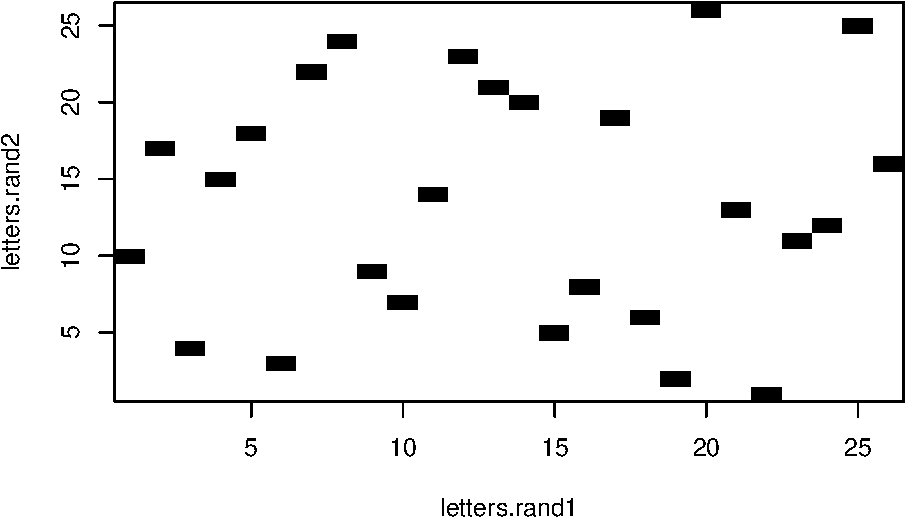
\includegraphics{lbrb_files/figure-latex/unnamed-chunk-185-1.pdf}

We can sort by the number of words using the sort() command

\begin{Shaded}
\begin{Highlighting}[]
\FunctionTok{sort}\NormalTok{(denguetable\_2)}
\end{Highlighting}
\end{Shaded}

\begin{verbatim}
## 
##   cg   ta   tc   gc   gt   cc   tt   ct   at   ac   gg   tg   ag   ca   ga   aa 
##  261  440  497  500  507  523  529  555  708  720  787  832  890  901  976 1108
\end{verbatim}

Let's save over the original object

\begin{Shaded}
\begin{Highlighting}[]
\NormalTok{denguetable\_2 }\OtherTok{\textless{}{-}} \FunctionTok{sort}\NormalTok{(denguetable\_2)}
\end{Highlighting}
\end{Shaded}

\begin{Shaded}
\begin{Highlighting}[]
\FunctionTok{barplot}\NormalTok{(denguetable\_2)}
\end{Highlighting}
\end{Shaded}

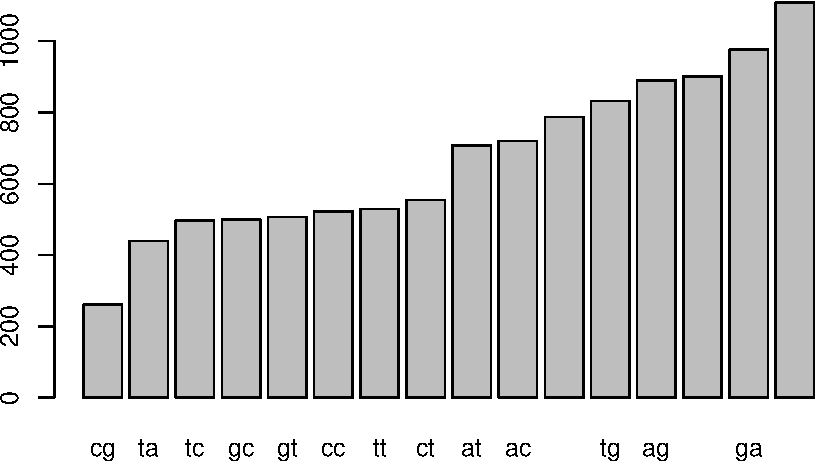
\includegraphics{lbrb_files/figure-latex/unnamed-chunk-188-1.pdf}

R will automatically try to optimize the appearance of the labels on the graph so you may not see all of them; no worries.

R can also make pie charts. Piecharts only really work when there are a few items being plots, like the four bases.

\begin{Shaded}
\begin{Highlighting}[]
\NormalTok{denguetable\_1 }\OtherTok{\textless{}{-}}\NormalTok{ seqinr}\SpecialCharTok{::}\FunctionTok{count}\NormalTok{(dengueseq\_vector,}\DecValTok{1}\NormalTok{)}
\end{Highlighting}
\end{Shaded}

Make a piechart with pie()

\begin{Shaded}
\begin{Highlighting}[]
\FunctionTok{pie}\NormalTok{(denguetable\_1)}
\end{Highlighting}
\end{Shaded}

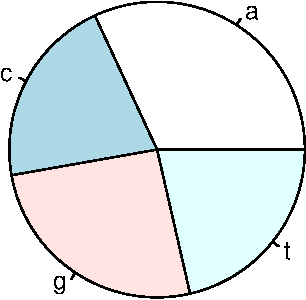
\includegraphics{lbrb_files/figure-latex/unnamed-chunk-190-1.pdf}

\hypertarget{summary-2}{%
\subsection{Summary}\label{summary-2}}

In this practical, have learned to use the following R functions:

length() for finding the length of a vector or list
table() for printing out a table of the number of occurrences of each type of item in a vector or list.
These functions belong to the standard installation of R.

You have also learnt the following R functions that belong to the SeqinR package:

GC() for calculating the GC content for a DNA sequence
count() for calculating the number of occurrences of DNA words of a particular length in a DNA sequence

\hypertarget{acknowledgements}{%
\section{Acknowledgements}\label{acknowledgements}}

This is a modification of \href{https://a-little-book-of-r-for-bioinformatics.readthedocs.io/en/latest/src/chapter1.html}{``DNA Sequence Statistics (1)''} from Avril Coghlan's \href{https://a-little-book-of-r-for-bioinformatics.readthedocs.io/en/latest/index.html}{\emph{A little book of R for bioinformatics.}}. Almost all of text and code was originally written by Dr.~Coghlan and distributed under the \href{https://creativecommons.org/licenses/by/3.0/us/}{Creative Commons 3.0} license.

In ``A little book\ldots{}'' Coghlan noted: ``Many of the ideas for the examples and exercises for this chapter were inspired by the Matlab case studies on Haemophilus influenzae (www.computational-genomics.net/case\_studies/haemophilus\_demo.html) and Bacteriophage lambda (\url{http://www.computational-genomics.net/case_studies/lambdaphage_demo.html}) from the website that accompanies the book Introduction to Computational Genomics: a case studies approach by Cristianini and Hahn (Cambridge University Press; www.computational-genomics.net/book/).''

\hypertarget{license}{%
\subsection{License}\label{license}}

The content in this book is licensed under a Creative Commons Attribution 3.0 License.

\url{https://creativecommons.org/licenses/by/3.0/us/}

\hypertarget{exercises}{%
\subsection{Exercises}\label{exercises}}

Answer the following questions, using the R package. For each question, please record your answer, and what you typed into R to get this answer.

Model answers to the exercises are given in Answers to the exercises on DNA Sequence Statistics (1).

\begin{enumerate}
\def\labelenumi{\arabic{enumi}.}
\tightlist
\item
  What are the last twenty nucleotides of the Dengue virus genome sequence?
\item
  What is the length in nucleotides of the genome sequence for the bacterium Mycobacterium leprae strain TN (accession NC\_002677)?
  Note: Mycobacterium leprae is a bacterium that is responsible for causing leprosy, which is classified by the WHO as a neglected tropical disease. As the genome sequence is a DNA sequence, if you are retrieving its sequence via the NCBI website, you will need to look for it in the NCBI Nucleotide database.
\item
  How many of each of the four nucleotides A, C, T and G, and any other symbols, are there in the Mycobacterium leprae TN genome sequence?
  Note: other symbols apart from the four nucleotides A/C/T/G may appear in a sequence. They correspond to positions in the sequence that are are not clearly one base or another and they are due, for example, to sequencing uncertainties. or example, the symbol `N' means `aNy base', while `R' means `A or G' (puRine). There is a table of symbols at www.bioinformatics.org/sms/iupac.html.
\item
  What is the GC content of the \emph{Mycobacterium leprae TN} genome sequence, when (i) all non-A/C/T/G nucleotides are included, (ii) non-A/C/T/G nucleotides are discarded?
  Hint: look at the help page for the GC() function to find out how it deals with non-A/C/T/G nucleotides.
\item
  How many of each of the four nucleotides A, C, T and G are there in the complement of the Mycobacterium leprae TN genome sequence? \emph{Hint}: you will first need to search for a function to calculate the complement of a sequence. Once you have found out what function to use, remember to use the help() function to find out what are the arguments (inputs) and results (outputs) of that function. How does the function deal with symbols other than the four nucleotides A, C, T and G? Are the numbers of As, Cs, Ts, and Gs in the complementary sequence what you would expect?
\item
  How many occurrences of the DNA words CC, CG and GC occur in the Mycobacterium leprae TN genome sequence?
\item
  How many occurrences of the DNA words CC, CG and GC occur in the (i) first 1000 and (ii) last 1000 nucleotides of the Mycobacterium leprae TN genome sequence?
  1.How can you check that the subsequence that you have looked at is 1000 nucleotides long?
\end{enumerate}

\hypertarget{downloading-protein-sequences-in-r}{%
\chapter{\texorpdfstring{Downloading protein sequences in \emph{R}}{Downloading protein sequences in R}}\label{downloading-protein-sequences-in-r}}

\textbf{By}: Avril Coghlan.

\textbf{Adapted, edited and expanded}: Nathan Brouwer under the Creative Commons 3.0 Attribution License \href{https://creativecommons.org/licenses/by/3.0/}{(CC BY 3.0)}.

\hypertarget{preliminaries-3}{%
\section{Preliminaries}\label{preliminaries-3}}

\begin{Shaded}
\begin{Highlighting}[]
\FunctionTok{library}\NormalTok{(compbio4all)}
\end{Highlighting}
\end{Shaded}

\hypertarget{retrieving-a-uniprot-protein-sequence-using-rentrez}{%
\section{Retrieving a UniProt protein sequence using rentrez}\label{retrieving-a-uniprot-protein-sequence-using-rentrez}}

We can use \texttt{entrez\_fetch()} to download protein sequences.

For example to retrieve the protein sequences for UniProt accessions Q9CD83 and A0PQ23, we type in R:

\begin{Shaded}
\begin{Highlighting}[]
\CommentTok{\# sequence 1: Q9CD83}
\NormalTok{leprae\_fasta }\OtherTok{\textless{}{-}}\NormalTok{ rentrez}\SpecialCharTok{::}\FunctionTok{entrez\_fetch}\NormalTok{(}\AttributeTok{db =} \StringTok{"protein"}\NormalTok{,}
                        \AttributeTok{id =} \StringTok{"Q9CD83"}\NormalTok{,}
                         \AttributeTok{rettype =} \StringTok{"fasta"}\NormalTok{)}
\CommentTok{\# sequence 2: OIN17619.1}
\NormalTok{ulcerans\_fasta }\OtherTok{\textless{}{-}}\NormalTok{ rentrez}\SpecialCharTok{::}\FunctionTok{entrez\_fetch}\NormalTok{(}\AttributeTok{db =} \StringTok{"protein"}\NormalTok{,}
                         \AttributeTok{id =} \StringTok{"OIN17619.1"}\NormalTok{,}
                         \AttributeTok{rettype =} \StringTok{"fasta"}\NormalTok{)}
\end{Highlighting}
\end{Shaded}

Display the contents of the \texttt{lepraeseq} FASTA file.

\begin{Shaded}
\begin{Highlighting}[]
\NormalTok{leprae\_fasta}
\end{Highlighting}
\end{Shaded}

\begin{verbatim}
## [1] ">sp|Q9CD83.1|PHBS_MYCLE RecName: Full=Chorismate pyruvate-lyase; AltName: Full=4-HB synthase; AltName: Full=p-hydroxybenzoic acid synthase\nMTNRTLSREEIRKLDRDLRILVATNGTLTRVLNVVANEEIVVDIINQQLLDVAPKIPELENLKIGRILQR\nDILLKGQKSGILFVAAESLIVIDLLPTAITTYLTKTHHPIGEIMAASRIETYKEDAQVWIGDLPCWLADY\nGYWDLPKRAVGRRYRIIAGGQPVIITTEYFLRSVFQDTPREELDRCQYSNDIDTRSGDRFVLHGRVFKNL\n\n"
\end{verbatim}

Let's clean these up to remove the header and new line characters usin the function \texttt{fasta\_cleaner()}.

\begin{Shaded}
\begin{Highlighting}[]
\NormalTok{leprae\_vector   }\OtherTok{\textless{}{-}} \FunctionTok{fasta\_cleaner}\NormalTok{(leprae\_fasta)}
\NormalTok{ulcerans\_vector }\OtherTok{\textless{}{-}} \FunctionTok{fasta\_cleaner}\NormalTok{(ulcerans\_fasta)}
\end{Highlighting}
\end{Shaded}

Examine the output using \texttt{length()}, \texttt{class()}, and \texttt{head()}:

\begin{Shaded}
\begin{Highlighting}[]
\FunctionTok{length}\NormalTok{(leprae\_vector)}
\FunctionTok{class}\NormalTok{(leprae\_vector)}
\FunctionTok{head}\NormalTok{(leprae\_vector, }\DecValTok{20}\NormalTok{)}
\end{Highlighting}
\end{Shaded}

\hypertarget{changes-to-database-entries}{%
\chapter{Changes to database entries}\label{changes-to-database-entries}}

Sometimes databases entries not linked or database entries get removed. When revising this chapter I had to update three of the accession numbers because the UniProt accessions in the original version weren't working for me.

For example the original UniProt entry included in the chapter
\href{https://www.uniprot.org/uniprot/E3M2K8}{E3M2K8} does not currently link directly to the NCBI entry for this same protein. Instead, I had to use the NCBI accession XP\_003109757.1. I'm not sure why this is.

Two accession numbers in the original version of this chapter appear to have been removed from UniProt because they were preliminary and perhaps did not meet the quality standards for UniProt. While the NCBI Gene and Protein are meant to be a record of \emph{all} sequence, NCBI RefSeq and UniProt are carefully curated to contain information that is consistent, accurate, and represents biological reality.

Searching the UniProt data base for two accessions in the original version of this chapter,
\href{https://www.uniprot.org/uniprot/E1FUV2}{E1FUV2} (\emph{Loa loa}) and
\href{https://www.uniprot.org/uniprot/A8NSK3}{A8NSK3}(\emph{Brugia malayi}), both yielded the result:
\textgreater{}``This entry is obsolete\ldots{} this entry was deleted. The protein sequence for this entry is available in UniParc. For previous versions of this entry, please look at its history.''

Looking at the history for the \emph{Loa loa} version of the protein we can see it was listed as ``unreviewed'' prior to it being pulled and has the note ``The sequence shown here is derived from an \ldots{} whole genome shotgun (WGS) entry which i preliminary data.'' (\url{https://www.uniprot.org/uniprot/E1FUV2.txt?version=9}). Once they got around to reviewing in, the curators at UniProt must have decided that it didn't meet the standards for inclusion in the database. The information about the sequence in other databases, however, was not deleted, just the entry in UniProt.

Most proteins are not experimentally studied in a lab, let alone their structure determined or their expression levels assessed. They are therefore predicted to be real based on their similarity to proteins that have been studied in model organisms.

To track down these sequences, I used BLAST. BLASTing the well-studied model organism \emph{C. elegans} version of the protein against the \emph{Loa loa} genome resulted in a hypothetical protein \href{https://blast.ncbi.nlm.nih.gov/Blast.cgi\#alnHdr_XP_020305433}{LOAG\_18175} a 93\% query coverage with C. elegans and 44\% identity. The accession number for this predicted protein in NCBI is \href{https://blast.ncbi.nlm.nih.gov/Blast.cgi\#alnHdr_XP_020305433}{XP\_020305433.1}. I similarly tracked down the accession for the \emph{Brugia malayi} version of the protein.

\hypertarget{sequence-dotplots-in-r}{%
\chapter{\texorpdfstring{Sequence dotplots in \emph{R}}{Sequence dotplots in R}}\label{sequence-dotplots-in-r}}

\textbf{By}: Avril Coghlan.

\textbf{Adapted, edited and expanded}: Nathan Brouwer under the Creative Commons 3.0 Attribution License \href{https://creativecommons.org/licenses/by/3.0/}{(CC BY 3.0)}.

\textbf{NOTE: I've added some new material that is rather terse and lacks explication.}

\hypertarget{preliminaries-4}{%
\section{Preliminaries}\label{preliminaries-4}}

\begin{Shaded}
\begin{Highlighting}[]
\FunctionTok{library}\NormalTok{(compbio4all)}
\end{Highlighting}
\end{Shaded}

\hypertarget{download-sequences}{%
\subsection{Download sequences}\label{download-sequences}}

As we did in the previous lesson on dotplots, we'll look at two sequences.

\begin{Shaded}
\begin{Highlighting}[]
\CommentTok{\# sequence 1: Q9CD83}
\NormalTok{leprae\_fasta }\OtherTok{\textless{}{-}}\NormalTok{ rentrez}\SpecialCharTok{::}\FunctionTok{entrez\_fetch}\NormalTok{(}\AttributeTok{db =} \StringTok{"protein"}\NormalTok{,}
                        \AttributeTok{id =} \StringTok{"Q9CD83"}\NormalTok{,}
                         \AttributeTok{rettype =} \StringTok{"fasta"}\NormalTok{)}
\CommentTok{\# sequence 2: OIN17619.1}
\NormalTok{ulcerans\_fasta }\OtherTok{\textless{}{-}}\NormalTok{ rentrez}\SpecialCharTok{::}\FunctionTok{entrez\_fetch}\NormalTok{(}\AttributeTok{db =} \StringTok{"protein"}\NormalTok{,}
                         \AttributeTok{id =} \StringTok{"OIN17619.1"}\NormalTok{,}
                         \AttributeTok{rettype =} \StringTok{"fasta"}\NormalTok{)}

\NormalTok{leprae\_vector   }\OtherTok{\textless{}{-}} \FunctionTok{fasta\_cleaner}\NormalTok{(leprae\_fasta)}
\NormalTok{ulcerans\_vector }\OtherTok{\textless{}{-}} \FunctionTok{fasta\_cleaner}\NormalTok{(ulcerans\_fasta)}
\end{Highlighting}
\end{Shaded}

\hypertarget{visualzing-two-identical-sequences}{%
\section{Visualzing two identical sequences}\label{visualzing-two-identical-sequences}}

To help build our intuition about dotplots we'll first look at some artificial examples. First, we'll see what happens when we make a dotplot comparing the alphabet versus itself. The build-in \texttt{LETTERS} object in R contains the alphabet from A to Z. This is a sequence with no repeats.

\begin{Shaded}
\begin{Highlighting}[]
\NormalTok{seqinr}\SpecialCharTok{::}\FunctionTok{dotPlot}\NormalTok{(LETTERS, }
\NormalTok{                LETTERS)}
\end{Highlighting}
\end{Shaded}

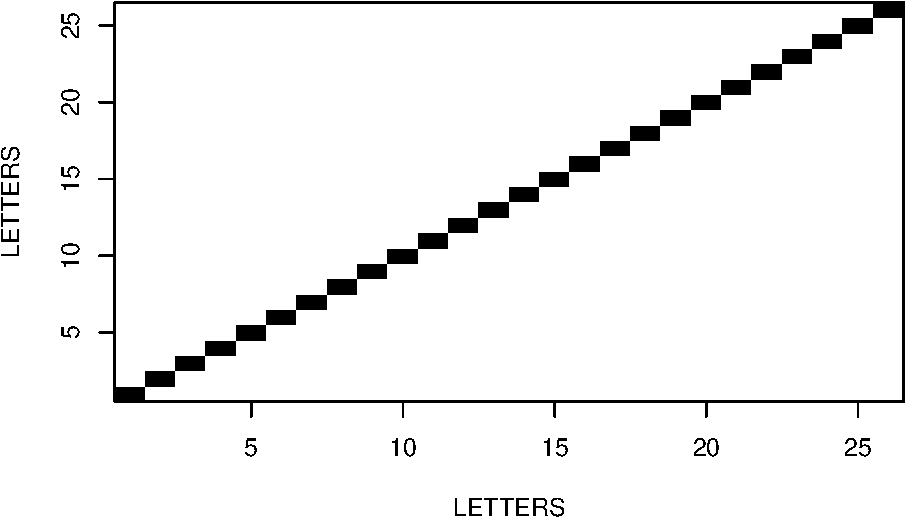
\includegraphics{lbrb_files/figure-latex/unnamed-chunk-199-1.pdf}

What we get is a perfect diagonal line.

\hypertarget{visualizing-repeats}{%
\section{Visualizing repeats}\label{visualizing-repeats}}

Now lets' make a sequence where the alphabet gets repeats twice

\begin{Shaded}
\begin{Highlighting}[]
\NormalTok{LETTERS.}\FloatTok{2.}\NormalTok{times }\OtherTok{\textless{}{-}} \FunctionTok{c}\NormalTok{(LETTERS,LETTERS)}

\NormalTok{seqinr}\SpecialCharTok{::}\FunctionTok{dotPlot}\NormalTok{(LETTERS.}\FloatTok{2.}\NormalTok{times, }
\NormalTok{                LETTERS.}\FloatTok{2.}\NormalTok{times)}
\end{Highlighting}
\end{Shaded}

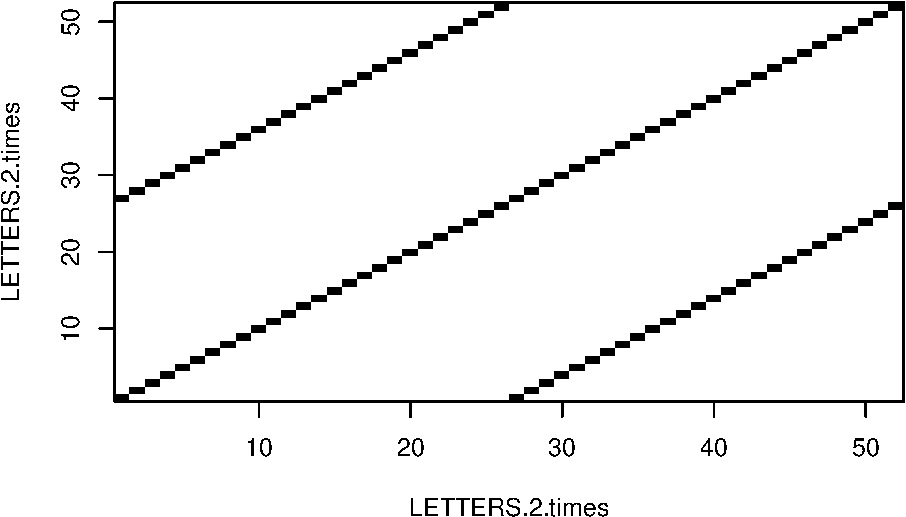
\includegraphics{lbrb_files/figure-latex/unnamed-chunk-200-1.pdf}

Note the diagonal lines.

Now 3 repeats

\begin{Shaded}
\begin{Highlighting}[]
\NormalTok{LETTERS.}\FloatTok{3.}\NormalTok{times }\OtherTok{\textless{}{-}} \FunctionTok{c}\NormalTok{(LETTERS,LETTERS,LETTERS)}

\NormalTok{seqinr}\SpecialCharTok{::}\FunctionTok{dotPlot}\NormalTok{(LETTERS.}\FloatTok{3.}\NormalTok{times, }
\NormalTok{                LETTERS.}\FloatTok{3.}\NormalTok{times)}
\end{Highlighting}
\end{Shaded}

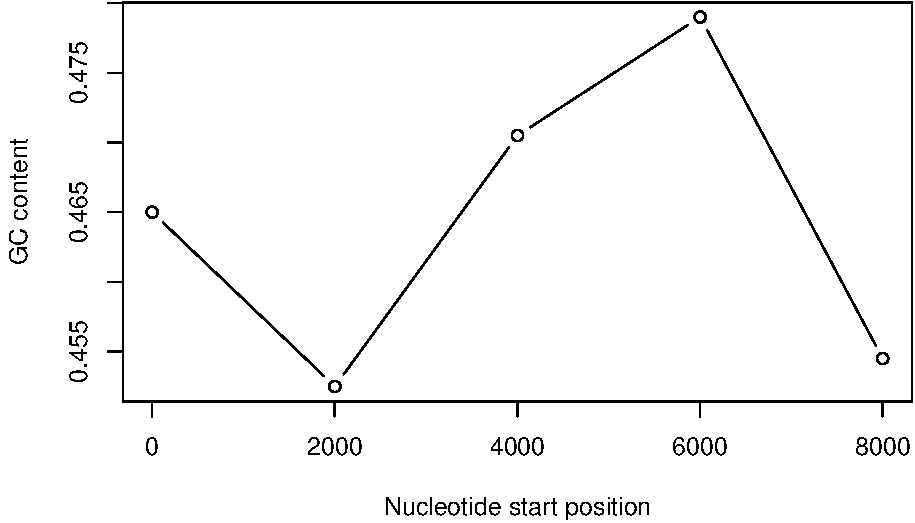
\includegraphics{lbrb_files/figure-latex/unnamed-chunk-201-1.pdf}

Here's another example of repeats.

Create sequence with repeats:

\begin{Shaded}
\begin{Highlighting}[]
\NormalTok{seq.repeat }\OtherTok{\textless{}{-}} \FunctionTok{c}\NormalTok{(}\StringTok{"A"}\NormalTok{,}\StringTok{"C"}\NormalTok{,}\StringTok{"D"}\NormalTok{,}\StringTok{"E"}\NormalTok{,}\StringTok{"F"}\NormalTok{,}\StringTok{"G"}\NormalTok{,}\StringTok{"H"}\NormalTok{,}\StringTok{"I"}\NormalTok{)}
\NormalTok{seq1 }\OtherTok{\textless{}{-}} \FunctionTok{rep}\NormalTok{(seq.repeat,}\DecValTok{3}\NormalTok{)}
\end{Highlighting}
\end{Shaded}

Make the dotplot:

\begin{Shaded}
\begin{Highlighting}[]
\NormalTok{seqinr}\SpecialCharTok{::}\FunctionTok{dotPlot}\NormalTok{(seq1, }
\NormalTok{                seq1)}
\end{Highlighting}
\end{Shaded}

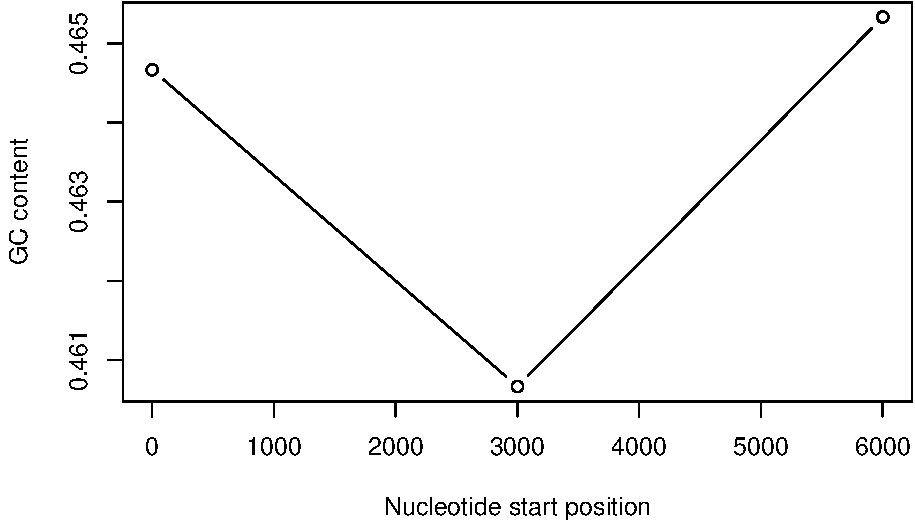
\includegraphics{lbrb_files/figure-latex/unnamed-chunk-203-1.pdf}

\hypertarget{inversions}{%
\section{Inversions}\label{inversions}}

See if you can figure out what's going on here.

\begin{Shaded}
\begin{Highlighting}[]
\NormalTok{LETTERS.}\FloatTok{3.}\NormalTok{times.with.invert }\OtherTok{\textless{}{-}} \FunctionTok{c}\NormalTok{(LETTERS,}\FunctionTok{rev}\NormalTok{(LETTERS),LETTERS)}

\NormalTok{seqinr}\SpecialCharTok{::}\FunctionTok{dotPlot}\NormalTok{(LETTERS.}\FloatTok{3.}\NormalTok{times, }
\NormalTok{                LETTERS.}\FloatTok{3.}\NormalTok{times.with.invert)}
\end{Highlighting}
\end{Shaded}

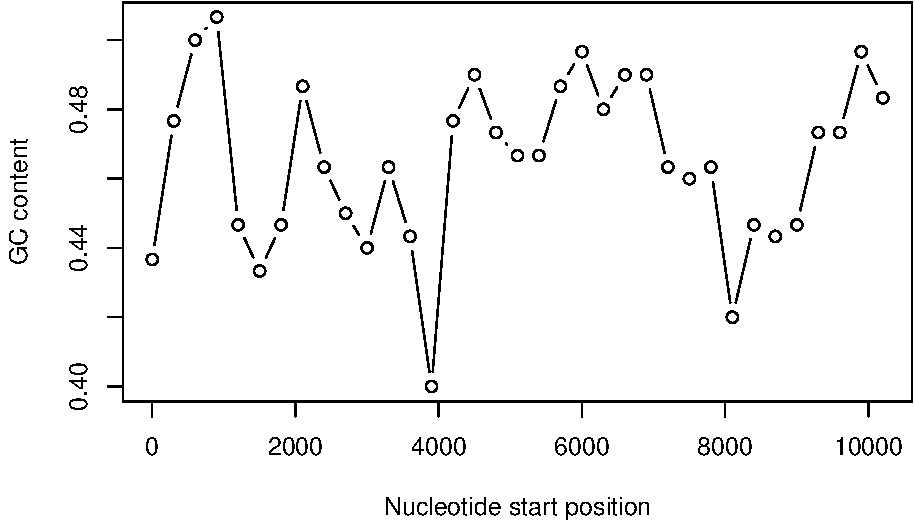
\includegraphics{lbrb_files/figure-latex/unnamed-chunk-204-1.pdf}

\hypertarget{translocations}{%
\section{Translocations}\label{translocations}}

See if you can figure out what's going on here.

\begin{Shaded}
\begin{Highlighting}[]
\NormalTok{seg1 }\OtherTok{\textless{}{-}}\NormalTok{ LETTERS[}\DecValTok{1}\SpecialCharTok{:}\DecValTok{8}\NormalTok{]}
\NormalTok{seg2 }\OtherTok{\textless{}{-}}\NormalTok{ LETTERS[}\DecValTok{9}\SpecialCharTok{:}\DecValTok{18}\NormalTok{]}
\NormalTok{seg3 }\OtherTok{\textless{}{-}}\NormalTok{ LETTERS[}\DecValTok{18}\SpecialCharTok{:}\DecValTok{26}\NormalTok{]}

\NormalTok{LETTERS.with.transloc }\OtherTok{\textless{}{-}} \FunctionTok{c}\NormalTok{(seg1,seg3,seg2)}

\NormalTok{seqinr}\SpecialCharTok{::}\FunctionTok{dotPlot}\NormalTok{(LETTERS, }
\NormalTok{                LETTERS.with.transloc)}
\end{Highlighting}
\end{Shaded}

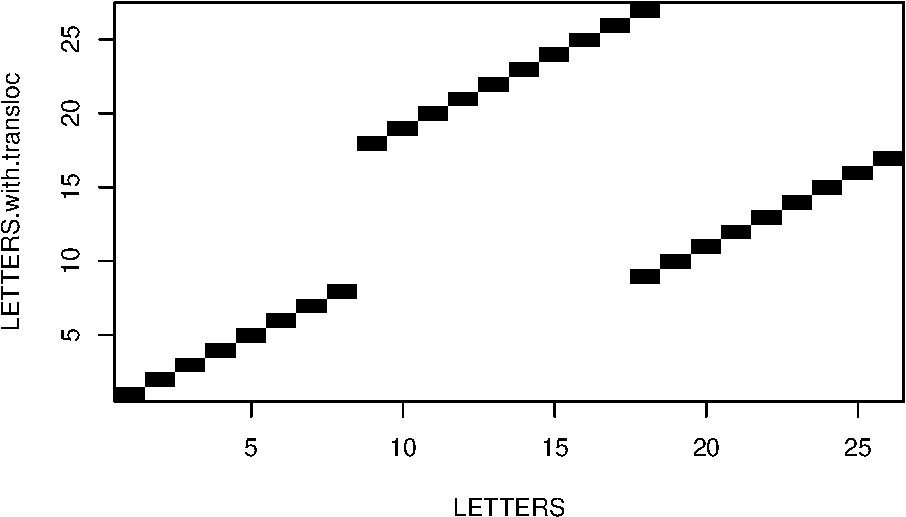
\includegraphics{lbrb_files/figure-latex/unnamed-chunk-205-1.pdf}

\hypertarget{random-sequence}{%
\section{Random sequence}\label{random-sequence}}

\begin{Shaded}
\begin{Highlighting}[]
\NormalTok{letters.rand1 }\OtherTok{\textless{}{-}} \FunctionTok{sample}\NormalTok{(}\AttributeTok{x =}\NormalTok{ LETTERS, }\AttributeTok{size =} \DecValTok{26}\NormalTok{, }\AttributeTok{replace =}\NormalTok{ F)}
\NormalTok{letters.rand2 }\OtherTok{\textless{}{-}} \FunctionTok{sample}\NormalTok{(}\AttributeTok{x =}\NormalTok{ LETTERS, }\AttributeTok{size =} \DecValTok{26}\NormalTok{, }\AttributeTok{replace =}\NormalTok{ F)}


\NormalTok{seqinr}\SpecialCharTok{::}\FunctionTok{dotPlot}\NormalTok{(letters.rand1, }
\NormalTok{                letters.rand2)}
\end{Highlighting}
\end{Shaded}

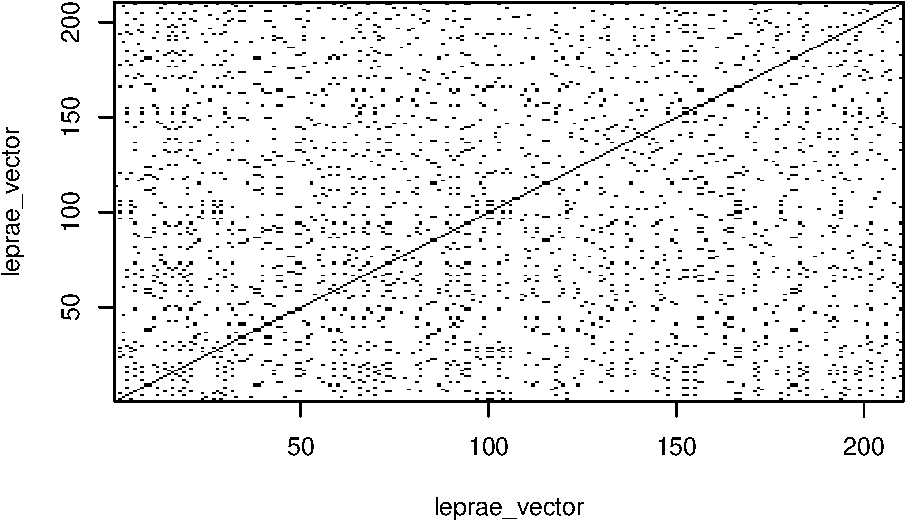
\includegraphics{lbrb_files/figure-latex/unnamed-chunk-206-1.pdf}

\hypertarget{comparing-two-real-sequences-using-a-dotplot}{%
\section{Comparing two real sequences using a dotplot}\label{comparing-two-real-sequences-using-a-dotplot}}

As a first step in comparing two protein, RNA or DNA sequences, it is a good idea to make a \textbf{dotplot}. A \textbf{dotplot} is a graphical method that allows the comparison of two protein or DNA sequences and identify regions of close similarity between them. A dotplot is essentially a two-dimensional matrix (like a grid), which has the sequences of the proteins being compared along the vertical and horizontal axes.

In order to make a simple dotplot to represent of the similarity between two sequences, individual cells in the matrix can be shaded black if residues are identical, so that matching sequence segments appear as runs of diagonal lines across the matrix. Identical proteins will have a line exactly on the main diagonal of the dotplot, that spans across the whole matrix.

For proteins that are not identical, but share regions of similarity, the dotplot will have shorter lines that may be on the \textbf{main diagonal}, or off the main diagonal of the matrix. In essence, a dotplot will reveal if there are any regions that are clearly very similar in two protein (or DNA) sequences.

We can create a dotplot for two sequences using the \texttt{dotPlot()} function in the \texttt{seqinr} package.

First, let's look at a dotplot created using only a single sequence. You'd never do this in practice, but it will give you a sense of what dotplots are doing.

\begin{Shaded}
\begin{Highlighting}[]
\NormalTok{seqinr}\SpecialCharTok{::}\FunctionTok{dotPlot}\NormalTok{(leprae\_vector, }
\NormalTok{                leprae\_vector)}
\end{Highlighting}
\end{Shaded}

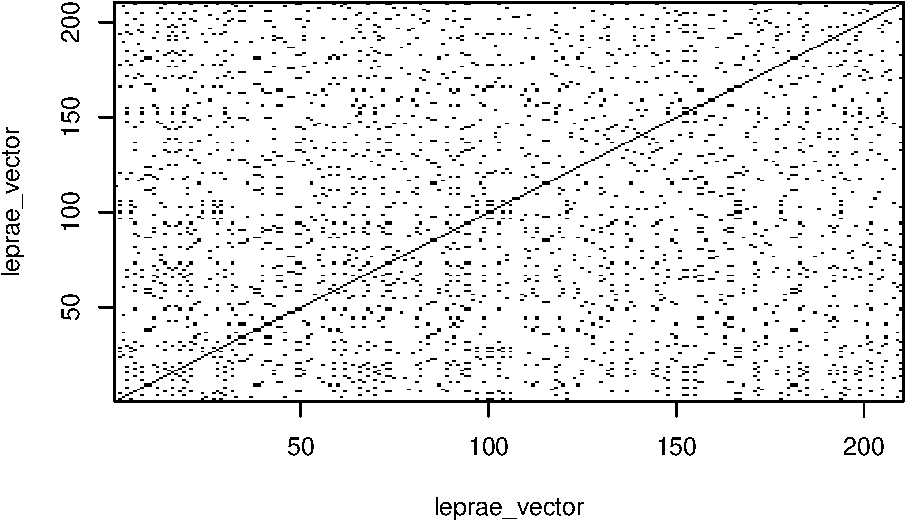
\includegraphics{lbrb_files/figure-latex/unnamed-chunk-207-1.pdf}

These two sequences are identical, so we have a very distinct diagonal line. But there's also other

Now we'll make a real dotplot of the \href{https://en.wikipedia.org/wiki/Chorismate_lyase}{chorismate lyase} proteins from two closely related species, \emph{Mycobacterium leprae} and \emph{Mycobacterium ulcerans}.

\begin{Shaded}
\begin{Highlighting}[]
\NormalTok{seqinr}\SpecialCharTok{::}\FunctionTok{dotPlot}\NormalTok{(leprae\_vector, }
\NormalTok{                ulcerans\_vector)}
\end{Highlighting}
\end{Shaded}

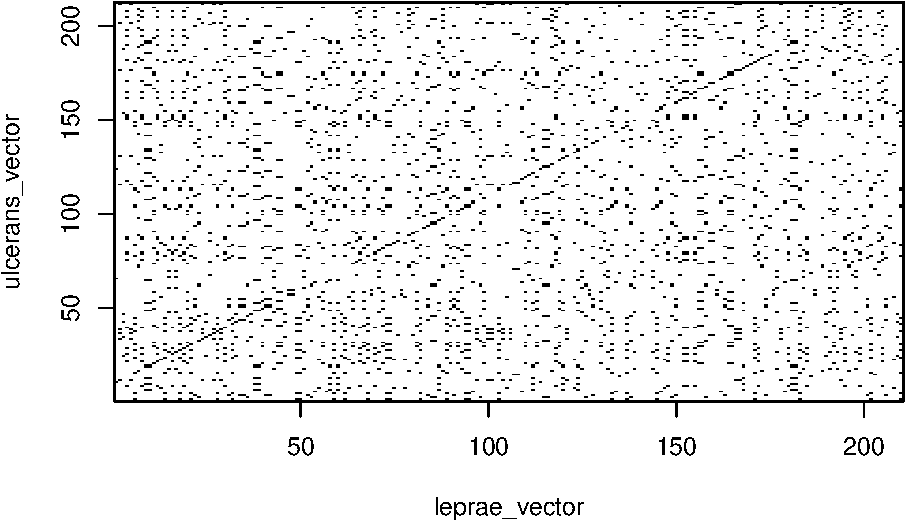
\includegraphics{lbrb_files/figure-latex/unnamed-chunk-208-1.pdf}

In the dotplot above, the \emph{M. leprae} sequence is plotted along the x-axis (horizontal axis), and the \emph{M. ulcerans} sequence is plotted along the y-axis (vertical axis). The dotplot displays a dot at points where there is an identical amino acid in the two sequences.

For example, if amino acid 53 in the \emph{M. leprae} sequence is the same amino acid (eg. ``W'') as amino acid 70 in the M. ulcerans sequence, then the dotplot will show a dot the position in the plot where x =50 and y =53.

In this case you can see a lot of dots along a diagonal line, which indicates that the two protein sequences contain many identical amino acids at the same (or very similar) positions along their lengths. This is what you would expect, because we know that these two proteins are \textbf{homologs} (related proteins) because they share a close evolutionary history.

\hypertarget{global-proteins-aligments-in-r}{%
\chapter{\texorpdfstring{Global proteins aligments in \emph{R}}{Global proteins aligments in R}}\label{global-proteins-aligments-in-r}}

\textbf{By}: Avril Coghlan.

\textbf{Adapted, edited and expanded}: Nathan Brouwer under the Creative Commons 3.0 Attribution License \href{https://creativecommons.org/licenses/by/3.0/}{(CC BY 3.0)}.

\hypertarget{preliminaries-5}{%
\section{Preliminaries}\label{preliminaries-5}}

\begin{Shaded}
\begin{Highlighting}[]
\FunctionTok{library}\NormalTok{(compbio4all)}
\FunctionTok{library}\NormalTok{(Biostrings)}
\end{Highlighting}
\end{Shaded}

\hypertarget{download-sequences-1}{%
\subsection{Download sequences}\label{download-sequences-1}}

As we did in the previous lesson on dotplots, we'll look at two sequences.

\begin{Shaded}
\begin{Highlighting}[]
\CommentTok{\# Download}
\DocumentationTok{\#\# sequence 1: Q9CD83}
\NormalTok{leprae\_fasta }\OtherTok{\textless{}{-}}\NormalTok{ rentrez}\SpecialCharTok{::}\FunctionTok{entrez\_fetch}\NormalTok{(}\AttributeTok{db =} \StringTok{"protein"}\NormalTok{,}
                        \AttributeTok{id =} \StringTok{"Q9CD83"}\NormalTok{,}
                         \AttributeTok{rettype =} \StringTok{"fasta"}\NormalTok{)}
\DocumentationTok{\#\# sequence 2: OIN17619.1}
\NormalTok{ulcerans\_fasta }\OtherTok{\textless{}{-}}\NormalTok{ rentrez}\SpecialCharTok{::}\FunctionTok{entrez\_fetch}\NormalTok{(}\AttributeTok{db =} \StringTok{"protein"}\NormalTok{,}
                         \AttributeTok{id =} \StringTok{"OIN17619.1"}\NormalTok{,}
                         \AttributeTok{rettype =} \StringTok{"fasta"}\NormalTok{)}

\CommentTok{\# clean}
\NormalTok{leprae\_vector   }\OtherTok{\textless{}{-}} \FunctionTok{fasta\_cleaner}\NormalTok{(leprae\_fasta)}
\NormalTok{ulcerans\_vector }\OtherTok{\textless{}{-}} \FunctionTok{fasta\_cleaner}\NormalTok{(ulcerans\_fasta)}
\end{Highlighting}
\end{Shaded}

\hypertarget{pairwise-global-alignment-of-dna-sequences-using-the-needleman-wunsch-algorithm}{%
\section{Pairwise global alignment of DNA sequences using the Needleman-Wunsch algorithm}\label{pairwise-global-alignment-of-dna-sequences-using-the-needleman-wunsch-algorithm}}

If you are studying a particular pair of genes or proteins, an important question is to what extent the two sequences are similar.

To quantify similarity, it is necessary to \textbf{align} the two sequences, and then you can calculate a similarity score based on the alignment.

There are two types of alignment in general. A \textbf{global alignment} is an alignment of the \emph{full} length of two sequences from beginning to end, for example, of two protein sequences or of two DNA sequences. A \textbf{local alignment} is an alignment of part of one sequence to part of another sequence; the parts the end up getting aligned are the most similar, and determined by the alignment algorithm.

The first step in computing a alignment (global or local) is to decide on a \textbf{scoring system}. For example, we may decide to give a score of +2 to a match and a penalty of -1 to a mismatch, and a penalty of -2 to a \textbf{gap} due to an \textbf{indexl}. Thus, for the alignment:

\begin{verbatim}
## [1] "G A A T T C"
\end{verbatim}

\begin{verbatim}
## [1] "G A T T - A"
\end{verbatim}

we would compute a score of

\begin{enumerate}
\def\labelenumi{\arabic{enumi}.}
\tightlist
\item
  G vs G = matchb = 2
\item
  A vs A = match = 2
\item
  A vs T = mismatch = -1
\item
  T vs T = match = 2
\item
  T vs - = gap = -2
\item
  C vs A = mismatch = 2
\end{enumerate}

So, the scores is 2 + 2 -1 + 2 -2 - 1 = 2.

Similarly, the score for the following alignment is 2 + 2 -2 + 2 + 2 -1 = 5:

\begin{verbatim}
## [1] "G A A T T C"
\end{verbatim}

\begin{verbatim}
## [1] "G A - T T A"
\end{verbatim}

The \textbf{scoring system} above can be represented by a \textbf{scoring matrix} (also known as a \textbf{substitution matrix}). The scoring matrix has one row and one column for each possible letter in our alphabet of letters (e.g.~4 rows and 4 columns for DNA and RNA sequences, 20 x 20 for amino acids). The (i,j) element of the matrix has a value of +2 in case of a match and -1 in case of a mismatch.

We can make a scoring matrix in R by using the \texttt{nucleotideSubstitutionMatrix()} function in the \texttt{Biostrings} package. \texttt{Biostrings} is part of a set of R packages for bioinformatics analysis known as \href{www.bioconductor.org/}{Bioconductor} (www.bioconductor.org/).

The arguments (inputs) for the \texttt{nucleotideSubstitutionMatrix()} function are the score that we want to assign to a match and the score that we want to assign to a mismatch. We can also specify that we want to use only the four letters representing the four nucleotides (ie. A, C, G, T) by setting \texttt{baseOnly=TRUE}, or whether we also want to use the letters that represent \textbf{ambiguous cases} where we are not sure what the nucleotide is (e.g.~`N' = A/C/G/T; ambiguous cases occur in some sequences due to sequencing errors or ambiguities).

To make a scoring matrix which assigns a score of +2 to a match and -1 to a mismatch, and store it in the variable \texttt{sigma}, we type:

\begin{Shaded}
\begin{Highlighting}[]
\CommentTok{\# make the matrix}
\NormalTok{sigma }\OtherTok{\textless{}{-}} \FunctionTok{nucleotideSubstitutionMatrix}\NormalTok{(}\AttributeTok{match =} \DecValTok{2}\NormalTok{, }
                                      \AttributeTok{mismatch =} \SpecialCharTok{{-}}\DecValTok{1}\NormalTok{, }
                                      \AttributeTok{baseOnly =} \ConstantTok{TRUE}\NormalTok{)}
\CommentTok{\# Print out the matrix}
\NormalTok{sigma }
\end{Highlighting}
\end{Shaded}

\begin{verbatim}
##    A  C  G  T
## A  2 -1 -1 -1
## C -1  2 -1 -1
## G -1 -1  2 -1
## T -1 -1 -1  2
\end{verbatim}

Instead of assigning the same penalty (e.g.~-8) to every gap position, it is common instead to assign a \textbf{gap opening penalty} to the first position in a gap (e.g.~-8), and a smaller \textbf{gap extension penalty} to every subsequent position in the same gap.

The reason for doing this is that it is likely that adjacent gap positions were created by the same insertion or deletion event, rather than by several independent insertion or deletion events. Therefore, we don't want to penalize a 3-letter gap (AAA---AAA) as much as we would penalize three separate 1-letter gaps (AA-A-A-AA), as the 3-letter gap may have arisen due to just one insertion or deletion event, while the 3 separate 1-letter gaps probably arose due to three independent insertion or deletion events.

For example, if we want to compute the score for a global alignment of two short DNA sequences `GAATTC' and `GATTA', we can use the \textbf{Needleman-Wunsch} algorithm to calculate the highest-scoring alignment using a particular scoring function.

The \texttt{pairwiseAlignment()} function in the Biostrings package finds the score for the optimal global alignment between two sequences using the Needleman-Wunsch algorithm, given a particular scoring system.

As arguments (inputs), \texttt{pairwiseAlignment()} takes

\begin{enumerate}
\def\labelenumi{\arabic{enumi}.}
\tightlist
\item
  the two sequences that you want to align,
\item
  the scoring matrix,
\item
  the gap opening penalty, and
\item
  the gap extension penalty.
\end{enumerate}

You can also tell the function that you want to just have the optimal global alignment's score by setting \texttt{scoreOnly\ =\ TRUE}, or that you want to have both the optimal global alignment and its score by setting \texttt{scoreOnly\ =\ FALSE}.

For example, let's find the score for the optimal global alignment between the sequences `GAATTC' and `GATTA'.

First, we'll store the sequences as \textbf{character vectors}:

\begin{Shaded}
\begin{Highlighting}[]
\NormalTok{s1 }\OtherTok{\textless{}{-}} \StringTok{"GAATTC"}
\NormalTok{s2 }\OtherTok{\textless{}{-}} \StringTok{"GATTA"}
\end{Highlighting}
\end{Shaded}

Now we'll align them:

\begin{Shaded}
\begin{Highlighting}[]
\NormalTok{globalAligns1s2 }\OtherTok{\textless{}{-}}\NormalTok{ Biostrings}\SpecialCharTok{::}\FunctionTok{pairwiseAlignment}\NormalTok{(s1, s2, }
                                                 \AttributeTok{substitutionMatrix =}\NormalTok{ sigma, }
                                                 \AttributeTok{gapOpening =} \SpecialCharTok{{-}}\DecValTok{2}\NormalTok{,}
                                                 \AttributeTok{gapExtension =} \SpecialCharTok{{-}}\DecValTok{8}\NormalTok{, }
                                                 \AttributeTok{scoreOnly =} \ConstantTok{FALSE}\NormalTok{)}
\end{Highlighting}
\end{Shaded}

The output:

\begin{Shaded}
\begin{Highlighting}[]
\NormalTok{globalAligns1s2 }
\end{Highlighting}
\end{Shaded}

\begin{verbatim}
## Global PairwiseAlignmentsSingleSubject (1 of 1)
## pattern: GAATTC
## subject: GA-TTA
## score: -3
\end{verbatim}

The above commands print out the optimal global alignment for the two sequences and its score.

\textbf{Note} we set \texttt{gapOpening} to be -2 and \texttt{gapExtension} to be -8, which means that the first position of a gap is assigned a score of -8 - 2= -10, and every subsequent position in a gap is given a score of -8. Here the alignment contains four matches, one mismatch, and one gap of length 1, so its score is (4\emph{2)+(1}-1)+(1*-10) = -3.

\hypertarget{pairwise-global-alignment-of-protein-sequences-using-the-needleman-wunsch-algorithm}{%
\section{Pairwise global alignment of protein sequences using the Needleman-Wunsch algorithm}\label{pairwise-global-alignment-of-protein-sequences-using-the-needleman-wunsch-algorithm}}

As well as DNA alignments, it is also possible to make alignments of protein sequences. In this case it is necessary to use a scoring matrix for amino acids rather than for nucleotides.

\hypertarget{protein-score-matrices}{%
\subsection{Protein score matrices}\label{protein-score-matrices}}

There are several well known scoring matrices that come with \emph{R}, such as the \textbf{BLOSUM} series of matrices. Different BLOSUM matrices exist, named with different numbers. BLOSUM with high numbers are designed for comparing closely related sequences, while BLOSUM with low numbers are designed for comparing evolutionarily distantly related sequences. For example, \textbf{BLOSUM62} is used for \textbf{less divergent alignments} (alignments of sequences that differ little), and \textbf{BLOSUM30} is used for more divergent alignments (alignments of sequences that differ a lot).

Many \emph{R} packages come with example data sets or data files and you use the \texttt{data()} function is used to load these data files. You can use the \texttt{data()} function to load a data set of BLOSUM matrices that comes with \texttt{Biostrings}

To load the BLOSUM50 matrix, we type:

\begin{Shaded}
\begin{Highlighting}[]
\FunctionTok{data}\NormalTok{(BLOSUM50)}
\NormalTok{BLOSUM50 }\CommentTok{\# Print out the data}
\end{Highlighting}
\end{Shaded}

\begin{verbatim}
##    A  R  N  D  C  Q  E  G  H  I  L  K  M  F  P  S  T  W  Y  V  B  Z  X  *
## A  5 -2 -1 -2 -1 -1 -1  0 -2 -1 -2 -1 -1 -3 -1  1  0 -3 -2  0 -2 -1 -1 -5
## R -2  7 -1 -2 -4  1  0 -3  0 -4 -3  3 -2 -3 -3 -1 -1 -3 -1 -3 -1  0 -1 -5
## N -1 -1  7  2 -2  0  0  0  1 -3 -4  0 -2 -4 -2  1  0 -4 -2 -3  4  0 -1 -5
## D -2 -2  2  8 -4  0  2 -1 -1 -4 -4 -1 -4 -5 -1  0 -1 -5 -3 -4  5  1 -1 -5
## C -1 -4 -2 -4 13 -3 -3 -3 -3 -2 -2 -3 -2 -2 -4 -1 -1 -5 -3 -1 -3 -3 -2 -5
## Q -1  1  0  0 -3  7  2 -2  1 -3 -2  2  0 -4 -1  0 -1 -1 -1 -3  0  4 -1 -5
## E -1  0  0  2 -3  2  6 -3  0 -4 -3  1 -2 -3 -1 -1 -1 -3 -2 -3  1  5 -1 -5
## G  0 -3  0 -1 -3 -2 -3  8 -2 -4 -4 -2 -3 -4 -2  0 -2 -3 -3 -4 -1 -2 -2 -5
## H -2  0  1 -1 -3  1  0 -2 10 -4 -3  0 -1 -1 -2 -1 -2 -3  2 -4  0  0 -1 -5
## I -1 -4 -3 -4 -2 -3 -4 -4 -4  5  2 -3  2  0 -3 -3 -1 -3 -1  4 -4 -3 -1 -5
## L -2 -3 -4 -4 -2 -2 -3 -4 -3  2  5 -3  3  1 -4 -3 -1 -2 -1  1 -4 -3 -1 -5
## K -1  3  0 -1 -3  2  1 -2  0 -3 -3  6 -2 -4 -1  0 -1 -3 -2 -3  0  1 -1 -5
## M -1 -2 -2 -4 -2  0 -2 -3 -1  2  3 -2  7  0 -3 -2 -1 -1  0  1 -3 -1 -1 -5
## F -3 -3 -4 -5 -2 -4 -3 -4 -1  0  1 -4  0  8 -4 -3 -2  1  4 -1 -4 -4 -2 -5
## P -1 -3 -2 -1 -4 -1 -1 -2 -2 -3 -4 -1 -3 -4 10 -1 -1 -4 -3 -3 -2 -1 -2 -5
## S  1 -1  1  0 -1  0 -1  0 -1 -3 -3  0 -2 -3 -1  5  2 -4 -2 -2  0  0 -1 -5
## T  0 -1  0 -1 -1 -1 -1 -2 -2 -1 -1 -1 -1 -2 -1  2  5 -3 -2  0  0 -1  0 -5
## W -3 -3 -4 -5 -5 -1 -3 -3 -3 -3 -2 -3 -1  1 -4 -4 -3 15  2 -3 -5 -2 -3 -5
## Y -2 -1 -2 -3 -3 -1 -2 -3  2 -1 -1 -2  0  4 -3 -2 -2  2  8 -1 -3 -2 -1 -5
## V  0 -3 -3 -4 -1 -3 -3 -4 -4  4  1 -3  1 -1 -3 -2  0 -3 -1  5 -4 -3 -1 -5
## B -2 -1  4  5 -3  0  1 -1  0 -4 -4  0 -3 -4 -2  0  0 -5 -3 -4  5  2 -1 -5
## Z -1  0  0  1 -3  4  5 -2  0 -3 -3  1 -1 -4 -1  0 -1 -2 -2 -3  2  5 -1 -5
## X -1 -1 -1 -1 -2 -1 -1 -2 -1 -1 -1 -1 -1 -2 -2 -1  0 -3 -1 -1 -1 -1 -1 -5
## * -5 -5 -5 -5 -5 -5 -5 -5 -5 -5 -5 -5 -5 -5 -5 -5 -5 -5 -5 -5 -5 -5 -5  1
\end{verbatim}

You can get a list of the available scoring matrices that come with the Biostrings package by using the data() function, which takes as an argument the name of the package for which you want to know the data sets that come with it:

\begin{Shaded}
\begin{Highlighting}[]
\FunctionTok{data}\NormalTok{(}\AttributeTok{package=}\StringTok{"Biostrings"}\NormalTok{)}
\end{Highlighting}
\end{Shaded}

Another well-known series of scoring matrices are the \textbf{PAM} matrices developed by \href{https://en.wikipedia.org/wiki/Margaret_Oakley_Dayhoff}{Margaret Dayhoff} and her team. These have largely been replaced by BLOSUM but are important for historical reasons because they represent one of the first major bioinformatics, computational biology, and phyolgenetics projects ever.

\hypertarget{example-protein-alignment}{%
\subsection{Example protein alignment}\label{example-protein-alignment}}

Let's find the optimal global alignment between the protein sequences ``PAWHEAE'' and ``HEAGAWGHEE'' using the Needleman-Wunsch algorithm using the BLOSUM50 matrix.

First, load the scoring matrix \texttt{BLOSUM50} and make vectors for the sequence

\begin{Shaded}
\begin{Highlighting}[]
\CommentTok{\# matrix}
\FunctionTok{data}\NormalTok{(BLOSUM50)}

\CommentTok{\# sequences}
\NormalTok{s3 }\OtherTok{\textless{}{-}} \StringTok{"PAWHEAE"}
\NormalTok{s4 }\OtherTok{\textless{}{-}} \StringTok{"HEAGAWGHEE"}
\end{Highlighting}
\end{Shaded}

Now do the alignments.

\begin{Shaded}
\begin{Highlighting}[]
\NormalTok{globalAligns3s4 }\OtherTok{\textless{}{-}} \FunctionTok{pairwiseAlignment}\NormalTok{(s3, s4,}
                                     \AttributeTok{substitutionMatrix =} \StringTok{"BLOSUM50"}\NormalTok{, }
                                     \AttributeTok{gapOpening =} \SpecialCharTok{{-}}\DecValTok{2}\NormalTok{,}
                                     \AttributeTok{gapExtension =} \SpecialCharTok{{-}}\DecValTok{8}\NormalTok{, }
                                     \AttributeTok{scoreOnly =} \ConstantTok{FALSE}\NormalTok{)}
\end{Highlighting}
\end{Shaded}

Look at the results:

\begin{Shaded}
\begin{Highlighting}[]
\NormalTok{globalAligns3s4 }\CommentTok{\# Print out the optimal global alignment and its score}
\end{Highlighting}
\end{Shaded}

\begin{verbatim}
## Global PairwiseAlignmentsSingleSubject (1 of 1)
## pattern: P---AWHEAE
## subject: HEAGAWGHEE
## score: -5
\end{verbatim}

We set \texttt{gapOpening} to be -2 and \texttt{gapExtension} to be -8, which means that the first position of a gap is assigned a score of -8-2=-10, and every subsequent position in a gap is given a score of -8. This means that the gap will be given a score of -10-8-8 = -26.

\hypertarget{aligning-uniprot-sequences}{%
\section{Aligning UniProt sequences}\label{aligning-uniprot-sequences}}

We discussed previously how you can search for UniProt accessions and retrieve the corresponding protein sequences, either via the UniProt website or using the \texttt{rentrez} package.

In the examples given above, we learned how to retrieve the sequences for the chorismate lyase proteins from \emph{Mycobacterium leprae} (UniProt Q9CD83) and \emph{Mycobacterium ulcerans} (UniProt A0PQ23), and read them into R, and store them as vectors lepraeseq and ulceransseq.

You can align these sequences using \texttt{pairwiseAlignment()} from the Biostrings package.

As its input, the \texttt{pairwiseAlignment()}function requires that the sequences be in the form of a single string (e.g.~``ACGTA''), rather than as a vector of characters (e.g.~a vector with the first element as ``A'', the second element as ``C'', etc.). Therefore, to align the \emph{M. leprae} and \emph{M. ulcerans} chorismate lyase proteins, we first need to convert the vectors lepraeeq and ulceransseq into strings. We can do this using the \texttt{paste()} function:

\begin{Shaded}
\begin{Highlighting}[]
\CommentTok{\# convert leprae\_vector to an object lepraeseq\_string}
\NormalTok{lepraeseq\_string }\OtherTok{\textless{}{-}}\FunctionTok{paste}\NormalTok{(leprae\_vector,}\AttributeTok{collapse =} \StringTok{""}\NormalTok{)    }

\CommentTok{\# convert ulcerans\_vector to an object ulceransseq\_string}
\NormalTok{ulceransseq\_string }\OtherTok{\textless{}{-}}\FunctionTok{paste}\NormalTok{(ulcerans\_vector,}\AttributeTok{collapse =} \StringTok{""}\NormalTok{) }
\end{Highlighting}
\end{Shaded}

Furthermore, pairwiseAlignment() requires that the sequences be stored as uppercase characters. Therefore, if they are not already in uppercase, we need to use the \texttt{toupper()} function to convert \texttt{lepraeseq\_string} and \texttt{ulceransseq\_string} to uppercase:

\begin{Shaded}
\begin{Highlighting}[]
\NormalTok{lepraeseq\_string   }\OtherTok{\textless{}{-}} \FunctionTok{toupper}\NormalTok{(lepraeseq\_string)}
\NormalTok{ulceransseq\_string }\OtherTok{\textless{}{-}} \FunctionTok{toupper}\NormalTok{(ulceransseq\_string)}
\end{Highlighting}
\end{Shaded}

Check the output

\begin{Shaded}
\begin{Highlighting}[]
\NormalTok{lepraeseq\_string }\CommentTok{\# Print out the content of "lepraeseq\_string"}
\end{Highlighting}
\end{Shaded}

\begin{verbatim}
## [1] "MTNRTLSREEIRKLDRDLRILVATNGTLTRVLNVVANEEIVVDIINQQLLDVAPKIPELENLKIGRILQRDILLKGQKSGILFVAAESLIVIDLLPTAITTYLTKTHHPIGEIMAASRIETYKEDAQVWIGDLPCWLADYGYWDLPKRAVGRRYRIIAGGQPVIITTEYFLRSVFQDTPREELDRCQYSNDIDTRSGDRFVLHGRVFKNL"
\end{verbatim}

We can now align the the \emph{M. leprae} and \emph{M. ulcerans} chorismate lyase protein sequences using the \texttt{pairwiseAlignment()} function:

\begin{Shaded}
\begin{Highlighting}[]
\NormalTok{globalAlignLepraeUlcerans }\OtherTok{\textless{}{-}}\NormalTok{ Biostrings}\SpecialCharTok{::}\FunctionTok{pairwiseAlignment}\NormalTok{(lepraeseq\_string, }
\NormalTok{                                               ulceransseq\_string,}
                                               \AttributeTok{substitutionMatrix =}\NormalTok{ BLOSUM50, }
                                               \AttributeTok{gapOpening =} \SpecialCharTok{{-}}\DecValTok{2}\NormalTok{, }
                                               \AttributeTok{gapExtension =} \SpecialCharTok{{-}}\DecValTok{8}\NormalTok{, }
                                               \AttributeTok{scoreOnly =} \ConstantTok{FALSE}\NormalTok{)}
\end{Highlighting}
\end{Shaded}

The output:

\begin{Shaded}
\begin{Highlighting}[]
\NormalTok{globalAlignLepraeUlcerans }\CommentTok{\# Print out the optimal global alignment and its score}
\end{Highlighting}
\end{Shaded}

\begin{verbatim}
## Global PairwiseAlignmentsSingleSubject (1 of 1)
## pattern: MT-----NR--T---LSREEIRKLDRDLRILVAT...DTPREELDRCQYSNDIDTRSGDRFVLHGRVFKNL
## subject: MLAVLPEKREMTECHLSDEEIRKLNRDLRILIAT...DNSREEPIRHQRS--VGT-SA-R---SGRSICT-
## score: 627
\end{verbatim}

As the alignment is very long, when you type \texttt{globalAlignLepraeUlcerans}, you only see the start and the end of the alignment. Therefore, we need to have a function to print out the whole alignment (see below).

\hypertarget{viewing-a-long-pairwise-alignment}{%
\section{Viewing a long pairwise alignment}\label{viewing-a-long-pairwise-alignment}}

If you want to view a long pairwise alignment such as that between the \emph{M. leprae} and \emph{M. ulerans} chorismate lyase proteins, it is convenient to print out the alignment in blocks.

The R function \texttt{print\_pairwise\_alignment()} below will do this for you:

\begin{Shaded}
\begin{Highlighting}[]
\FunctionTok{print\_pairwise\_alignment}\NormalTok{(globalAlignLepraeUlcerans, }\DecValTok{60}\NormalTok{)}
\end{Highlighting}
\end{Shaded}

\begin{verbatim}
## [1] "MT-----NR--T---LSREEIRKLDRDLRILVATNGTLTRVLNVVANEEIVVDIINQQLL 50"
## [1] "MLAVLPEKREMTECHLSDEEIRKLNRDLRILIATNGTLTRILNVLANDEIVVEIVKQQIQ 60"
## [1] " "
## [1] "DVAPKIPELENLKIGRILQRDILLKGQKSGILFVAAESLIVIDLLPTAITTYLTKTHHPI 110"
## [1] "DAAPEMDGCDHSSIGRVLRRDIVLKGRRSGIPFVAAESFIAIDLLPPEIVASLLETHRPI 120"
## [1] " "
## [1] "GEIMAASRIETYKEDAQVWIGDLPCWLADYGYWDLPKRAVGRRYRIIAGGQPVIITTEYF 170"
## [1] "GEVMAASCIETFKEEAKVWAGESPAWLELDRRRNLPPKVVGRQYRVIAEGRPVIIITEYF 180"
## [1] " "
## [1] "LRSVFQDTPREELDRCQYSNDIDTRSGDRFVLHGRVFKN 230"
## [1] "LRSVFEDNSREEPIRHQRS--VGT-SA-R---SGRSICT 233"
## [1] " "
\end{verbatim}

The position in the protein of the amino acid that is at the end of each line of the printed alignment is shown after the end of the line. For example, the first line of the alignment above finishes at amino acid position 50 in the \emph{M. leprae} protein and also at amino acid position 60 in the \emph{M. ulcerans} protein. Becaues there as a difference of 60-50 = 10 bases, there must be 10 insertions in the \emph{M. leprae} to get it to line up. Count the number of dashes in the sequence to see how many there are.

\hypertarget{local-protein-aligments-in-r}{%
\chapter{\texorpdfstring{Local protein aligments in \emph{R}}{Local protein aligments in R}}\label{local-protein-aligments-in-r}}

\textbf{By}: Avril Coghlan.

\textbf{Adapted, edited and expanded}: Nathan Brouwer under the Creative Commons 3.0 Attribution License \href{https://creativecommons.org/licenses/by/3.0/}{(CC BY 3.0)}.

\hypertarget{preliminaries-6}{%
\section{Preliminaries}\label{preliminaries-6}}

\begin{Shaded}
\begin{Highlighting}[]
\FunctionTok{library}\NormalTok{(compbio4all)}
\FunctionTok{library}\NormalTok{(Biostrings)}
\end{Highlighting}
\end{Shaded}

\hypertarget{download-sequences-2}{%
\subsection{Download sequences}\label{download-sequences-2}}

As we did in the previous lesson on dotplots, we'll look at two sequences.

\begin{Shaded}
\begin{Highlighting}[]
\CommentTok{\# Download}
\DocumentationTok{\#\# sequence 1: Q9CD83}
\NormalTok{leprae\_fasta }\OtherTok{\textless{}{-}}\NormalTok{ rentrez}\SpecialCharTok{::}\FunctionTok{entrez\_fetch}\NormalTok{(}\AttributeTok{db =} \StringTok{"protein"}\NormalTok{,}
                        \AttributeTok{id =} \StringTok{"Q9CD83"}\NormalTok{,}
                         \AttributeTok{rettype =} \StringTok{"fasta"}\NormalTok{)}
\DocumentationTok{\#\# sequence 2: OIN17619.1}
\NormalTok{ulcerans\_fasta }\OtherTok{\textless{}{-}}\NormalTok{ rentrez}\SpecialCharTok{::}\FunctionTok{entrez\_fetch}\NormalTok{(}\AttributeTok{db =} \StringTok{"protein"}\NormalTok{,}
                         \AttributeTok{id =} \StringTok{"OIN17619.1"}\NormalTok{,}
                         \AttributeTok{rettype =} \StringTok{"fasta"}\NormalTok{)}

\CommentTok{\# clean}
\NormalTok{leprae\_vector   }\OtherTok{\textless{}{-}} \FunctionTok{fasta\_cleaner}\NormalTok{(leprae\_fasta)}
\NormalTok{ulcerans\_vector }\OtherTok{\textless{}{-}} \FunctionTok{fasta\_cleaner}\NormalTok{(ulcerans\_fasta)}

\CommentTok{\# convert leprae\_vector to an object lepraeseq\_string}
\NormalTok{lepraeseq\_string }\OtherTok{\textless{}{-}}\FunctionTok{paste}\NormalTok{(leprae\_vector,}\AttributeTok{collapse =} \StringTok{""}\NormalTok{)    }

\CommentTok{\# convert ulcerans\_vector to an object ulceransseq\_string}
\NormalTok{ulceransseq\_string }\OtherTok{\textless{}{-}}\FunctionTok{paste}\NormalTok{(ulcerans\_vector,}\AttributeTok{collapse =} \StringTok{""}\NormalTok{) }
\end{Highlighting}
\end{Shaded}

\hypertarget{pairwise-local-alignment-of-protein-sequences-using-the-smith-waterman-algorithm}{%
\section{Pairwise local alignment of protein sequences using the Smith-Waterman algorithm}\label{pairwise-local-alignment-of-protein-sequences-using-the-smith-waterman-algorithm}}

You can use the \texttt{pairwiseAlignment()} function to find the optimal \textbf{local alignment} of two sequences, that is the best alignment of parts (\textbf{subsequences}) of those sequences, by using the \texttt{type=local} argument in \texttt{pairwiseAlignment()}. This uses the \textbf{\href{https://en.wikipedia.org/wiki/Smith\%E2\%80\%93Waterman_algorithm}{Smith-Waterman algorithm}} for local alignment. This is the classic bioinformatics algorithm for finding optimal local alignments. (We'll discuss updated approaches when we get into \textbf{database searches} with \textbf{BLAST}, the **Basic, Local Alignment Search Tool* that is the workhorse of many day-to-day bioinformatics tasks).

For example, to find the best local alignment between the \emph{M. leprae} and \emph{M. ulcerans} chorismate lyase proteins, we can run:

\begin{Shaded}
\begin{Highlighting}[]
\CommentTok{\# load scoring matrix}
\FunctionTok{data}\NormalTok{(BLOSUM50)}

\CommentTok{\# run alignment}
\NormalTok{localAlignLepraeUlcerans }\OtherTok{\textless{}{-}} \FunctionTok{pairwiseAlignment}\NormalTok{(lepraeseq\_string, }
\NormalTok{                                              ulceransseq\_string,}
                                              \AttributeTok{substitutionMatrix =}\NormalTok{ BLOSUM50, }
                                              \AttributeTok{gapOpening =} \SpecialCharTok{{-}}\DecValTok{2}\NormalTok{, }
                                              \AttributeTok{gapExtension =} \SpecialCharTok{{-}}\DecValTok{8}\NormalTok{, }
                                              \AttributeTok{scoreOnly =} \ConstantTok{FALSE}\NormalTok{, }
                                              \AttributeTok{type=}\StringTok{"local"}\NormalTok{)  }\CommentTok{\# \textless{}= type = "local !}
\end{Highlighting}
\end{Shaded}

Print out the optimal local alignment and its score

\begin{Shaded}
\begin{Highlighting}[]
\NormalTok{localAlignLepraeUlcerans }
\end{Highlighting}
\end{Shaded}

\begin{verbatim}
## Local PairwiseAlignmentsSingleSubject (1 of 1)
## pattern:  [1] MTNRTLSREEIRKLDRDLRILVATNGTLTRVL...TEYFLRSVFQDTPREELDRCQYSNDIDTRSG
## subject: [11] MTECHLSDEEIRKLNRDLRILIATNGTLTRIL...TEYFLRSVFEDNSREEPIRHQRSVGTSARSG
## score: 761
\end{verbatim}

As before, we can print out the full alignment with \texttt{print\_pairwise\_alignment()}:

\begin{Shaded}
\begin{Highlighting}[]
\FunctionTok{print\_pairwise\_alignment}\NormalTok{(localAlignLepraeUlcerans, }\DecValTok{60}\NormalTok{)}
\end{Highlighting}
\end{Shaded}

\begin{verbatim}
## [1] "MTNRTLSREEIRKLDRDLRILVATNGTLTRVLNVVANEEIVVDIINQQLLDVAPKIPELE 60"
## [1] "MTECHLSDEEIRKLNRDLRILIATNGTLTRILNVLANDEIVVEIVKQQIQDAAPEMDGCD 60"
## [1] " "
## [1] "NLKIGRILQRDILLKGQKSGILFVAAESLIVIDLLPTAITTYLTKTHHPIGEIMAASRIE 120"
## [1] "HSSIGRVLRRDIVLKGRRSGIPFVAAESFIAIDLLPPEIVASLLETHRPIGEVMAASCIE 120"
## [1] " "
## [1] "TYKEDAQVWIGDLPCWLADYGYWDLPKRAVGRRYRIIAGGQPVIITTEYFLRSVFQDTPR 180"
## [1] "TFKEEAKVWAGESPAWLELDRRRNLPPKVVGRQYRVIAEGRPVIIITEYFLRSVFEDNSR 180"
## [1] " "
## [1] "EELDRCQYSNDIDTRSG 240"
## [1] "EEPIRHQRSVGTSARSG 240"
## [1] " "
\end{verbatim}

We see that the optimal local alignment is quite similar to the optimal global alignment in this case, except that it excludes a short region of poorly aligned sequence at the start and at the ends of the two proteins.

\hypertarget{alignment-by-eye-in-r}{%
\chapter{Alignment by eye in R}\label{alignment-by-eye-in-r}}

\textbf{By} Nathan Brouwer

\hypertarget{preliminaries-7}{%
\section{Preliminaries}\label{preliminaries-7}}

\hypertarget{packages}{%
\subsection{Packages}\label{packages}}

\begin{Shaded}
\begin{Highlighting}[]
\FunctionTok{library}\NormalTok{(compbio4all)}
\FunctionTok{library}\NormalTok{(Biostrings)}
\end{Highlighting}
\end{Shaded}

\hypertarget{data}{%
\subsection{Data}\label{data}}

\begin{Shaded}
\begin{Highlighting}[]
\FunctionTok{data}\NormalTok{(}\StringTok{"BLOSUM62"}\NormalTok{)}
\end{Highlighting}
\end{Shaded}

Let's do an alignment between two parts of a shroom protein. We'll look at part of the ASD2 domain of Shroom 3. We'll look at human shroom (hShrm3) and call this the ``Query'' sequence. We'll use mouse shroom (mShrm3) as the ``subject'' or ``target''. (The accession number for human shroom 3 is NP\_065910.3)

\begin{Shaded}
\begin{Highlighting}[]
\NormalTok{hShrm3  }\OtherTok{\textless{}{-}} \StringTok{"EPEREPEWRDRPGSP"}

\NormalTok{mShrm3   }\OtherTok{\textless{}{-}} \StringTok{"EAEREASWSEDRPGT"}
\end{Highlighting}
\end{Shaded}

Use nchar() to see how many characters are in them

We can make a little matrix and look at how they align using the rbind() function, which stands for ``row bind''

\begin{Shaded}
\begin{Highlighting}[]
\FunctionTok{rbind}\NormalTok{(hShrm3,}
\NormalTok{      mShrm3)}
\end{Highlighting}
\end{Shaded}

\begin{verbatim}
##        [,1]             
## hShrm3 "EPEREPEWRDRPGSP"
## mShrm3 "EAEREASWSEDRPGT"
\end{verbatim}

Assign this to an object called shrms

\begin{Shaded}
\begin{Highlighting}[]
\NormalTok{shrms }\OtherTok{\textless{}{-}} \FunctionTok{rbind}\NormalTok{(hShrm3, mShrm3)}
\end{Highlighting}
\end{Shaded}

What type of object is shrms?

How big is it? See if you can guess first before using R to check

If we want to do an alignment by eye it would help if instead of having all the letters stuck together they were separated. We would do this by hand but it would require a lot of typing:

\begin{Shaded}
\begin{Highlighting}[]
\NormalTok{hShrm3\_alt }\OtherTok{\textless{}{-}} \FunctionTok{c}\NormalTok{(}\StringTok{"E"}\NormalTok{,}\StringTok{"P"}\NormalTok{,}\StringTok{"E"}\NormalTok{,}\StringTok{"R"}\NormalTok{,}\StringTok{"E"}\NormalTok{,}\StringTok{"P"}\NormalTok{,}\StringTok{"E"}\NormalTok{,}\StringTok{"W"}\NormalTok{,}\StringTok{"R"}\NormalTok{,}\StringTok{"D"}\NormalTok{,}\StringTok{"R"}\NormalTok{,}\StringTok{"P"}\NormalTok{,}\StringTok{"G"}\NormalTok{,}\StringTok{"S"}\NormalTok{,}\StringTok{"P"}\NormalTok{)}

\NormalTok{mShrm3\_alt }\OtherTok{\textless{}{-}} \FunctionTok{c}\NormalTok{(}\StringTok{"E"}\NormalTok{,}\StringTok{"A"}\NormalTok{,}\StringTok{"E"}\NormalTok{,}\StringTok{"R"}\NormalTok{,}\StringTok{"E"}\NormalTok{,}\StringTok{"A"}\NormalTok{,}\StringTok{"S"}\NormalTok{,}\StringTok{"W"}\NormalTok{,}\StringTok{"S"}\NormalTok{,}\StringTok{"E"}\NormalTok{,}\StringTok{"D"}\NormalTok{,}\StringTok{"R"}\NormalTok{,}\StringTok{"P"}\NormalTok{,}\StringTok{"G"}\NormalTok{,}\StringTok{"T"}\NormalTok{)}
\end{Highlighting}
\end{Shaded}

One thing that is annoying about R is that vectors have ``length'' but no dimension. Compare the output of the length() command and dim() command when called on hShrm3\_alt

\begin{Shaded}
\begin{Highlighting}[]
\CommentTok{\# run length()}


\CommentTok{\# run dim()}
\end{Highlighting}
\end{Shaded}

Use is, is.vector, length, is.character, and n.char on hShrm3 and hShrm3\_alt. How is hShrm3 (``EPEREPEWRDRPGSP'') different from hShrm3\_alt? Can you figure out why nchar() is doing what its doing?

\begin{Shaded}
\begin{Highlighting}[]
\CommentTok{\# run is() on hShrm3 AND hShrm3\_alt}


\CommentTok{\# run is.vector on hShrm3 AND hShrm3\_alt}


\CommentTok{\# do this for the rest of the commands}
\end{Highlighting}
\end{Shaded}

Typing all this stuff out is a pain. Instead of typing all those commas to make hShrm3\_alt we could take hShrm3 and have \emph{R} do the work for us. Lots of people work with \textbf{character data} (data make up of alphabetic and other characters that can NOT be interpreted as numbers) so there are lots of functions for manipulating characters. We'll use the \texttt{strsplit()} function.

If we just all strsplit() on the hShrm3 object we get something a little annoying.

\begin{Shaded}
\begin{Highlighting}[]
\FunctionTok{strsplit}\NormalTok{(hShrm3, }\AttributeTok{split =} \StringTok{""}\NormalTok{)}
\end{Highlighting}
\end{Shaded}

\begin{verbatim}
## [[1]]
##  [1] "E" "P" "E" "R" "E" "P" "E" "W" "R" "D" "R" "P" "G" "S" "P"
\end{verbatim}

Note that the output above is on too lines, and the first line is \texttt{{[}{[}1{]}{]}}.

Ok, what's up?

Assign the thing we just made to an object called hShrm3\_vec for ``hShrm3 vector''.

\begin{Shaded}
\begin{Highlighting}[]
\NormalTok{hShrm3\_vec }\OtherTok{\textless{}{-}} \FunctionTok{strsplit}\NormalTok{(hShrm3, }\AttributeTok{split =} \StringTok{""}\NormalTok{)}
\end{Highlighting}
\end{Shaded}

Now figure out what the heck it ``is'':

If you used the right command to figure out what it \textbf{is} (hint) the first thing you see is ``list.'' Lists are rather complex \textbf{data structures} in R because they aren't the kind of thing you run in to if you just have experience working in a spreadsheet. Lists allow you to make collections of different R objects. For now you just need to know that they exist; we'll run into them again later. For now, we want to get rid of this listy-ness of our R object. We can do this with the function unlist(). Call unlist() on your hShrm3\_vec object and re-assign it to the same object hShrm3\_vec, eg, run
hShrm3\_vec \textless- unlist(hShrm3\_vec)

\begin{Shaded}
\begin{Highlighting}[]
\NormalTok{hShrm3\_vec }\OtherTok{\textless{}{-}} \FunctionTok{unlist}\NormalTok{(hShrm3\_vec)}
\end{Highlighting}
\end{Shaded}

Now we need to repeat these steps for the mouse shroom sequence.

\begin{Shaded}
\begin{Highlighting}[]
\CommentTok{\# split up mShrm3 with strsplit()}
\NormalTok{mShrm3\_vec }\OtherTok{\textless{}{-}} \FunctionTok{strsplit}\NormalTok{(mShrm3, }\AttributeTok{split =} \StringTok{""}\NormalTok{)}

\CommentTok{\# unlist it with unlist()}
\NormalTok{mShrm3\_vec }\OtherTok{\textless{}{-}} \FunctionTok{unlist}\NormalTok{(mShrm3\_vec)}
\end{Highlighting}
\end{Shaded}

Something that is useful once you get good at reading R code is that you can wrap functions within functions. So instead of doing this in separate steps I could just do this:

\begin{Shaded}
\begin{Highlighting}[]
\NormalTok{hShrm3\_vec }\OtherTok{\textless{}{-}} \FunctionTok{unlist}\NormalTok{(}\FunctionTok{strsplit}\NormalTok{(hShrm3, }\AttributeTok{split =} \StringTok{""}\NormalTok{))}
\NormalTok{mShrm3\_vec }\OtherTok{\textless{}{-}} \FunctionTok{unlist}\NormalTok{(}\FunctionTok{strsplit}\NormalTok{(mShrm3, }\AttributeTok{split =} \StringTok{""}\NormalTok{))}
\end{Highlighting}
\end{Shaded}

Before moving on confirm that these two factors are the same length. If they aren't R will get angry

\begin{Shaded}
\begin{Highlighting}[]
\CommentTok{\# length of hShrm3\_vec}

\CommentTok{\# length of mShrm3\_vec}
\end{Highlighting}
\end{Shaded}

Now let's make a little matrix so we can think about aligning these sequences. The rbind() function binds two rows together into a matrix.

\begin{Shaded}
\begin{Highlighting}[]
\FunctionTok{rbind}\NormalTok{(hShrm3\_vec, mShrm3\_vec)}
\end{Highlighting}
\end{Shaded}

\begin{verbatim}
##            [,1] [,2] [,3] [,4] [,5] [,6] [,7] [,8] [,9] [,10] [,11] [,12] [,13]
## hShrm3_vec "E"  "P"  "E"  "R"  "E"  "P"  "E"  "W"  "R"  "D"   "R"   "P"   "G"  
## mShrm3_vec "E"  "A"  "E"  "R"  "E"  "A"  "S"  "W"  "S"  "E"   "D"   "R"   "P"  
##            [,14] [,15]
## hShrm3_vec "S"   "P"  
## mShrm3_vec "G"   "T"
\end{verbatim}

For what we want to do next aligning them vertically will actually work better. We can align them as columns using cbind(), which stands for ``column bind''

\begin{Shaded}
\begin{Highlighting}[]
\FunctionTok{cbind}\NormalTok{(hShrm3\_vec, mShrm3\_vec)}
\end{Highlighting}
\end{Shaded}

\begin{verbatim}
##       hShrm3_vec mShrm3_vec
##  [1,] "E"        "E"       
##  [2,] "P"        "A"       
##  [3,] "E"        "E"       
##  [4,] "R"        "R"       
##  [5,] "E"        "E"       
##  [6,] "P"        "A"       
##  [7,] "E"        "S"       
##  [8,] "W"        "W"       
##  [9,] "R"        "S"       
## [10,] "D"        "E"       
## [11,] "R"        "D"       
## [12,] "P"        "R"       
## [13,] "G"        "P"       
## [14,] "S"        "G"       
## [15,] "P"        "T"
\end{verbatim}

Save that to an object called shrm

\begin{Shaded}
\begin{Highlighting}[]
\FunctionTok{cbind}\NormalTok{(hShrm3\_vec, mShrm3\_vec)}
\end{Highlighting}
\end{Shaded}

\begin{verbatim}
##       hShrm3_vec mShrm3_vec
##  [1,] "E"        "E"       
##  [2,] "P"        "A"       
##  [3,] "E"        "E"       
##  [4,] "R"        "R"       
##  [5,] "E"        "E"       
##  [6,] "P"        "A"       
##  [7,] "E"        "S"       
##  [8,] "W"        "W"       
##  [9,] "R"        "S"       
## [10,] "D"        "E"       
## [11,] "R"        "D"       
## [12,] "P"        "R"       
## [13,] "G"        "P"       
## [14,] "S"        "G"       
## [15,] "P"        "T"
\end{verbatim}

\begin{Shaded}
\begin{Highlighting}[]
\NormalTok{shrm }\OtherTok{\textless{}{-}} \FunctionTok{cbind}\NormalTok{(hShrm3\_vec, mShrm3\_vec)}
\end{Highlighting}
\end{Shaded}

The most basic way to do an alignment is to determine the which bases are identical and to score those as 1, and anything that is mismatched score as 0. From this you can determine \textbf{percent identity}.

A handy way to do this quickly in R is to use the ifelse() command. What you can do is tell it to do this: ``IF a base in the first sequence the same as the aligned base in the second sequence, return a value of 1, ELSE return a value of 0.''

I'll do a really transparent example. First, let me make some very simple objects with just a single letter in them.

\begin{Shaded}
\begin{Highlighting}[]
\NormalTok{aa1 }\OtherTok{\textless{}{-}} \StringTok{"A"}
\NormalTok{aa2 }\OtherTok{\textless{}{-}} \StringTok{"A"}
\NormalTok{aa3 }\OtherTok{\textless{}{-}} \StringTok{"W"}
\end{Highlighting}
\end{Shaded}

What kind of object have I just made? Use is, is.vector, length, dim, and is.matrix. Can you understand why you get the results that you do?

Now let me use ifelse(). First, let me check if aa1 is the same as aa2, an if they R, return a value of 1, else return a value of 0

\begin{Shaded}
\begin{Highlighting}[]
\FunctionTok{ifelse}\NormalTok{(aa1 }\SpecialCharTok{==}\NormalTok{ aa2, }\AttributeTok{yes =}  \DecValTok{1}\NormalTok{, }\AttributeTok{no =} \DecValTok{0}\NormalTok{)}
\end{Highlighting}
\end{Shaded}

\begin{verbatim}
## [1] 1
\end{verbatim}

The first part of the function asks a true/false question: is aa1 the same as aa2? Note that it is TWO equals signs

This is a \textbf{logical comparison} or \textbf{logical test} in R. It would work on its own outside of ifelse, like this:

\begin{Shaded}
\begin{Highlighting}[]
\NormalTok{aa1 }\SpecialCharTok{==}\NormalTok{ aa2}
\end{Highlighting}
\end{Shaded}

\begin{verbatim}
## [1] TRUE
\end{verbatim}

Now compare aa1 and aa2. First try the logical test

Now try the ifelse() command

Something that is very hand in R is that it can process things in a series. First, let's turn our single amino acids into some sequences.

\begin{Shaded}
\begin{Highlighting}[]
\NormalTok{seq1 }\OtherTok{\textless{}{-}} \FunctionTok{c}\NormalTok{(aa1, aa2, aa3)}
\NormalTok{seq2 }\OtherTok{\textless{}{-}} \FunctionTok{c}\NormalTok{(aa3, aa2, aa1)}
\end{Highlighting}
\end{Shaded}

Do you know what kind of R object we just made? Run an appropriate check

Now let's compare these two sequences. First a logical comparison. Can you tell what this code is doing?

\begin{Shaded}
\begin{Highlighting}[]
\NormalTok{seq1 }\SpecialCharTok{==}\NormalTok{ seq2}
\end{Highlighting}
\end{Shaded}

\begin{verbatim}
## [1] FALSE  TRUE FALSE
\end{verbatim}

What is going on here? It might help to line everything up using rbind() to make a little matrix. First, save the output of the logical comparison to an R object

\begin{Shaded}
\begin{Highlighting}[]
\NormalTok{identical }\OtherTok{\textless{}{-}}\NormalTok{ seq1}\SpecialCharTok{==}\NormalTok{seq2}
\end{Highlighting}
\end{Shaded}

Now stack the two sequences and the logical comparison into a matrix

\begin{Shaded}
\begin{Highlighting}[]
\FunctionTok{rbind}\NormalTok{(seq1, seq2, identical)}
\end{Highlighting}
\end{Shaded}

\begin{verbatim}
##           [,1]    [,2]   [,3]   
## seq1      "A"     "A"    "W"    
## seq2      "W"     "A"    "A"    
## identical "FALSE" "TRUE" "FALSE"
\end{verbatim}

We can also run ifelse() on the two sequences

\begin{Shaded}
\begin{Highlighting}[]
\FunctionTok{ifelse}\NormalTok{(seq1 }\SpecialCharTok{==}\NormalTok{ seq2, }\AttributeTok{yes =} \DecValTok{1}\NormalTok{, }\AttributeTok{no =} \DecValTok{0}\NormalTok{)}
\end{Highlighting}
\end{Shaded}

\begin{verbatim}
## [1] 0 1 0
\end{verbatim}

Save this output to an object called align.score for ``alignment score''

\begin{Shaded}
\begin{Highlighting}[]
\NormalTok{align.score }\OtherTok{\textless{}{-}} \FunctionTok{ifelse}\NormalTok{(seq1 }\SpecialCharTok{==}\NormalTok{ seq2, }\AttributeTok{yes =} \DecValTok{1}\NormalTok{, }\AttributeTok{no =} \DecValTok{0}\NormalTok{)}
\end{Highlighting}
\end{Shaded}

Now stack everything up into a matrix using rbind

\begin{Shaded}
\begin{Highlighting}[]
\FunctionTok{rbind}\NormalTok{(seq1, seq2, identical, align.score )}
\end{Highlighting}
\end{Shaded}

\begin{verbatim}
##             [,1]    [,2]   [,3]   
## seq1        "A"     "A"    "W"    
## seq2        "W"     "A"    "A"    
## identical   "FALSE" "TRUE" "FALSE"
## align.score "0"     "1"    "0"
\end{verbatim}

Now let's try this on our shroom vectors. First, do a logical comparison of the hShrm3\_vec vector and the mShrm3\_vec vector. Remember there are two equals signs (==)

Now use ifelse() to assign a 1 to a match and a 0 to a mismatch.

Again, can you describe what's going on here?

Again we can make a little matrix with rbind(). I'm going to embed the ifelse() function within rbind(); this might be a little dense but see if you can figure out what each separate command is.

\begin{Shaded}
\begin{Highlighting}[]
\FunctionTok{rbind}\NormalTok{(hShrm3\_vec, }
\NormalTok{      mShrm3\_vec,}
      \AttributeTok{identical =}\NormalTok{ hShrm3\_vec }\SpecialCharTok{==}\NormalTok{ mShrm3\_vec,}
      \AttributeTok{score=} \FunctionTok{ifelse}\NormalTok{(hShrm3\_vec }\SpecialCharTok{==}\NormalTok{ mShrm3\_vec,}\AttributeTok{yes =} \DecValTok{1}\NormalTok{, }\AttributeTok{no =} \DecValTok{0}\NormalTok{ ))}
\end{Highlighting}
\end{Shaded}

\begin{verbatim}
##            [,1]   [,2]    [,3]   [,4]   [,5]   [,6]    [,7]    [,8]   [,9]   
## hShrm3_vec "E"    "P"     "E"    "R"    "E"    "P"     "E"     "W"    "R"    
## mShrm3_vec "E"    "A"     "E"    "R"    "E"    "A"     "S"     "W"    "S"    
## identical  "TRUE" "FALSE" "TRUE" "TRUE" "TRUE" "FALSE" "FALSE" "TRUE" "FALSE"
## score      "1"    "0"     "1"    "1"    "1"    "0"     "0"     "1"    "0"    
##            [,10]   [,11]   [,12]   [,13]   [,14]   [,15]  
## hShrm3_vec "D"     "R"     "P"     "G"     "S"     "P"    
## mShrm3_vec "E"     "D"     "R"     "P"     "G"     "T"    
## identical  "FALSE" "FALSE" "FALSE" "FALSE" "FALSE" "FALSE"
## score      "0"     "0"     "0"     "0"     "0"     "0"
\end{verbatim}

If we want the total score we can assign the results of ifelse() to an object

\begin{Shaded}
\begin{Highlighting}[]
\NormalTok{scores }\OtherTok{\textless{}{-}}\FunctionTok{ifelse}\NormalTok{(hShrm3\_vec }\SpecialCharTok{==}\NormalTok{ mShrm3\_vec,}\AttributeTok{yes =} \DecValTok{1}\NormalTok{, }\AttributeTok{no =} \DecValTok{0}\NormalTok{ )}
\end{Highlighting}
\end{Shaded}

I can then total up the score with sum()

\begin{Shaded}
\begin{Highlighting}[]
\FunctionTok{sum}\NormalTok{(scores)}
\end{Highlighting}
\end{Shaded}

\begin{verbatim}
## [1] 5
\end{verbatim}

I can easily call up the number of amino acids with length(). Do that below

Percent identity is a common statistic when comparing sequences. If my score is 5 and my total number of residues is 15 my percent identity is:

\begin{Shaded}
\begin{Highlighting}[]
\DecValTok{5}\SpecialCharTok{/}\DecValTok{15}
\end{Highlighting}
\end{Shaded}

\begin{verbatim}
## [1] 0.3333333
\end{verbatim}

I can do this directly on the objects like this

\begin{Shaded}
\begin{Highlighting}[]
\FunctionTok{sum}\NormalTok{(scores)}\SpecialCharTok{/}\FunctionTok{length}\NormalTok{(scores)}
\end{Highlighting}
\end{Shaded}

\begin{verbatim}
## [1] 0.3333333
\end{verbatim}

We can do this sort of scoring on sequences in a matrix or data frame. Remember that we made a matrix called shrm with our two sequences in it. Matrices and dataframes are very similar, but its usually easier to work with dataframes. We can convert the matrix to a dataframe like this

\begin{Shaded}
\begin{Highlighting}[]
\NormalTok{shrm }\OtherTok{\textless{}{-}} \FunctionTok{data.frame}\NormalTok{(shrm, }\AttributeTok{stringsAsFactors =}\NormalTok{ F)}
\end{Highlighting}
\end{Shaded}

There's a lot relate to the ``stringsAsFactors = F''; basically it makes sure we are working with raw character data.

Calling summary() on the shrm dataframe can confirm that its character data:

\begin{Shaded}
\begin{Highlighting}[]
\FunctionTok{summary}\NormalTok{(shrm)}
\end{Highlighting}
\end{Shaded}

\begin{verbatim}
##   hShrm3_vec         mShrm3_vec       
##  Length:15          Length:15         
##  Class :character   Class :character  
##  Mode  :character   Mode  :character
\end{verbatim}

You can call up the human shroom 3 columns with this code: shrm{[}, ``hShrm3\_vec''{]}. try it below

How would you call up the other column with mouse shroom?

One tricky thin about R is that you can access the column of dataframes in more than one way. You can get the first column also using the dollar sign

\begin{Shaded}
\begin{Highlighting}[]
\NormalTok{shrm}\SpecialCharTok{$}\NormalTok{hShrm3\_vec}
\end{Highlighting}
\end{Shaded}

\begin{verbatim}
##  [1] "E" "P" "E" "R" "E" "P" "E" "W" "R" "D" "R" "P" "G" "S" "P"
\end{verbatim}

Note that even though we're calling a column, R prints it out left to right like a row.

We can do a logical comparisons of the two columns like this:

\begin{Shaded}
\begin{Highlighting}[]
\NormalTok{shrm[, }\StringTok{"hShrm3\_vec"}\NormalTok{] }\SpecialCharTok{==}\NormalTok{ shrm[,}\StringTok{"mShrm3\_vec"}\NormalTok{]}
\end{Highlighting}
\end{Shaded}

\begin{verbatim}
##  [1]  TRUE FALSE  TRUE  TRUE  TRUE FALSE FALSE  TRUE FALSE FALSE FALSE FALSE
## [13] FALSE FALSE FALSE
\end{verbatim}

Can you re-write this using the dollar sign notation? Try it below

Now let's use ifelse() on these two columns

\begin{Shaded}
\begin{Highlighting}[]
\FunctionTok{ifelse}\NormalTok{(shrm[, }\StringTok{"hShrm3\_vec"}\NormalTok{] }\SpecialCharTok{==}\NormalTok{ shrm[,}\StringTok{"mShrm3\_vec"}\NormalTok{], }\AttributeTok{yes =} \DecValTok{1}\NormalTok{, }\AttributeTok{no =} \DecValTok{0}\NormalTok{)}
\end{Highlighting}
\end{Shaded}

\begin{verbatim}
##  [1] 1 0 1 1 1 0 0 1 0 0 0 0 0 0 0
\end{verbatim}

Rewrite the code above using dollar sign notation

We can add this information to the dataframe like this

\begin{Shaded}
\begin{Highlighting}[]
\NormalTok{shrm}\SpecialCharTok{$}\NormalTok{identical }\OtherTok{\textless{}{-}} \FunctionTok{ifelse}\NormalTok{(shrm[, }\StringTok{"hShrm3\_vec"}\NormalTok{] }\SpecialCharTok{==}\NormalTok{ shrm[,}\StringTok{"mShrm3\_vec"}\NormalTok{], }\AttributeTok{yes =} \DecValTok{1}\NormalTok{, }\AttributeTok{no =} \DecValTok{0}\NormalTok{)}
\end{Highlighting}
\end{Shaded}

Now what do we have? Call up the dataframe shrm we just made:

Now call summary on it. What types of data are each variable?

Comparing an alignment to a scoring matrix by hand is a lot of work, so there's a function called \texttt{score\_alignment()} in the \texttt{compbio4all} package which can do basic comparisons. The function has the following arguments

\begin{itemize}
\tightlist
\item
  seq.df = A dataframe with aligned sequences in columns
\item
  seq1 = the name of the column with a sequence in it; name must be in quotes
\item
  seq2 = the other, aligned sequence
\item
  gap.penalty = -10
\end{itemize}

Running the function returns a dataframe with a new column called ``score''.

\begin{Shaded}
\begin{Highlighting}[]
\NormalTok{shrm }\OtherTok{\textless{}{-}}\FunctionTok{score\_alignment}\NormalTok{(}\AttributeTok{seq.df =}\NormalTok{ shrm, }
                \AttributeTok{seq1=}  \StringTok{"hShrm3\_vec"}\NormalTok{,  }\CommentTok{\#note the quotation marks}
                \AttributeTok{seq2 =} \StringTok{"mShrm3\_vec"}\NormalTok{,}
                \AttributeTok{sub.mat =}\NormalTok{ BLOSUM62,}
                \AttributeTok{gap.penalty =}  \SpecialCharTok{{-}}\DecValTok{10}\NormalTok{)}
\end{Highlighting}
\end{Shaded}

We can call the sum() function on the score column of the shrm dataframe to calculate the overall score for the alignment. This is a metric that tells use how good the alignment is based on the number of identical residues in the sequence, how different any mutations are from the original residue, and how many gaps there are.

\begin{Shaded}
\begin{Highlighting}[]
\FunctionTok{sum}\NormalTok{(shrm}\SpecialCharTok{$}\NormalTok{score)}
\end{Highlighting}
\end{Shaded}

\begin{verbatim}
## [1] 23
\end{verbatim}

I happen to know that we can make this alignment better if we add a gap. I'll do it by hand because I don't have a function yet to do it automatically. I'll put a gap into the human shroom 3 sequence (hShrm3\_alt) after the ``W'' that's about in the middle of the sequence.

\begin{Shaded}
\begin{Highlighting}[]
\NormalTok{hShrm3\_alt  }\OtherTok{\textless{}{-}} \FunctionTok{c}\NormalTok{(}\StringTok{"E"}\NormalTok{,}\StringTok{"P"}\NormalTok{,}\StringTok{"E"}\NormalTok{,}\StringTok{"R"}\NormalTok{,}\StringTok{"E"}\NormalTok{,}\StringTok{"P"}\NormalTok{,}\StringTok{"E"}\NormalTok{,}\StringTok{"W"}\NormalTok{,}\StringTok{"{-}"}\NormalTok{,}\StringTok{"R"}\NormalTok{,}\StringTok{"D"}\NormalTok{,}\StringTok{"R"}\NormalTok{,}\StringTok{"P"}\NormalTok{,}\StringTok{"G"}\NormalTok{,}\StringTok{"S"}\NormalTok{,}\StringTok{"P"}\NormalTok{)}
\end{Highlighting}
\end{Shaded}

Using an appropriate function, confirm that the insertion has made the sequence longer (hint: its not nchar)

Now we'll do the other sequence. To make this work we need to add an insertion to the end of the mouse sequence (mShrm3\_alt) so that the two sequences are the same length.

\begin{Shaded}
\begin{Highlighting}[]
\NormalTok{mShrm3\_alt  }\OtherTok{\textless{}{-}} \FunctionTok{c}\NormalTok{(}\StringTok{"E"}\NormalTok{,}\StringTok{"A"}\NormalTok{,}\StringTok{"E"}\NormalTok{,}\StringTok{"R"}\NormalTok{,}\StringTok{"E"}\NormalTok{,}\StringTok{"A"}\NormalTok{,}\StringTok{"S"}\NormalTok{,}\StringTok{"W"}\NormalTok{,}\StringTok{"S"}\NormalTok{,}\StringTok{"E"}\NormalTok{,}\StringTok{"D"}\NormalTok{,}\StringTok{"R"}\NormalTok{,}\StringTok{"P"}\NormalTok{,}\StringTok{"G"}\NormalTok{,}\StringTok{"T"}\NormalTok{,}\StringTok{"{-}"}\NormalTok{)}
\end{Highlighting}
\end{Shaded}

Again, check that this sequence is longer than it was before

A handy trick is to do a \textbf{logical comparison} to check that the two vectors are the same. Run the following code and see if you can interpret what is going on. Remember that the double equals sign == carries out a logical comparison that returns TRUE if two values are the same.

\begin{Shaded}
\begin{Highlighting}[]
\FunctionTok{length}\NormalTok{(hShrm3\_alt) }\SpecialCharTok{==} \FunctionTok{length}\NormalTok{(mShrm3\_alt)}
\end{Highlighting}
\end{Shaded}

\begin{verbatim}
## [1] TRUE
\end{verbatim}

Now, for a challenge, see if you can figure out what's going on here

\begin{Shaded}
\begin{Highlighting}[]
\NormalTok{hShrm3\_alt }\SpecialCharTok{==}\NormalTok{ mShrm3\_alt}
\end{Highlighting}
\end{Shaded}

\begin{verbatim}
##  [1]  TRUE FALSE  TRUE  TRUE  TRUE FALSE FALSE  TRUE FALSE FALSE  TRUE  TRUE
## [13]  TRUE  TRUE FALSE FALSE
\end{verbatim}

It might be easier if we stack thing in to a little matrix with rbind(). I've put a lot of stuff in the rbind() function but see if you can figure it out.

\begin{Shaded}
\begin{Highlighting}[]
\FunctionTok{rbind}\NormalTok{(}\AttributeTok{hShrm3\_alt =}\NormalTok{ hShrm3\_alt,}
      \AttributeTok{mShrm3\_alt =}\NormalTok{ mShrm3\_alt,}
      \AttributeTok{identical =}\NormalTok{ hShrm3\_alt }\SpecialCharTok{==}\NormalTok{ mShrm3\_alt)}
\end{Highlighting}
\end{Shaded}

\begin{verbatim}
##            [,1]   [,2]    [,3]   [,4]   [,5]   [,6]    [,7]    [,8]   [,9]   
## hShrm3_alt "E"    "P"     "E"    "R"    "E"    "P"     "E"     "W"    "-"    
## mShrm3_alt "E"    "A"     "E"    "R"    "E"    "A"     "S"     "W"    "S"    
## identical  "TRUE" "FALSE" "TRUE" "TRUE" "TRUE" "FALSE" "FALSE" "TRUE" "FALSE"
##            [,10]   [,11]  [,12]  [,13]  [,14]  [,15]   [,16]  
## hShrm3_alt "R"     "D"    "R"    "P"    "G"    "S"     "P"    
## mShrm3_alt "E"     "D"    "R"    "P"    "G"    "T"     "-"    
## identical  "FALSE" "TRUE" "TRUE" "TRUE" "TRUE" "FALSE" "FALSE"
\end{verbatim}

Now let's compare these two sequences by scoring them. First, we'll put them into a dataframe using data.frame(). We'll call the object shrm.gap.

\begin{Shaded}
\begin{Highlighting}[]
\NormalTok{shrm.gap }\OtherTok{\textless{}{-}}\FunctionTok{data.frame}\NormalTok{(hShrm3\_alt,}
\NormalTok{                      mShrm3\_alt, }
                      \AttributeTok{stringsAsFactors =}\NormalTok{ F)}
\end{Highlighting}
\end{Shaded}

Run an appropriate function to confirm that this is a dataframe

Check what the size of the dataframe is:

Now look at the full dataframe

Now run a function to just look at the top of the dataframe:

Run a function to just look at the bottom of the dataframe

Ok, we have a sense of what we're working with. Let's calculate the score

\begin{Shaded}
\begin{Highlighting}[]
\NormalTok{shrm.gap }\OtherTok{\textless{}{-}} \FunctionTok{score\_alignment}\NormalTok{(shrm.gap, }
                     \AttributeTok{seq1=}  \StringTok{"hShrm3\_alt"}\NormalTok{,}
                     \AttributeTok{seq2 =} \StringTok{"mShrm3\_alt"}\NormalTok{,}
                     \AttributeTok{sub.mat=}\NormalTok{ BLOSUM62,}
                     \AttributeTok{gap.penalty =}\SpecialCharTok{{-}}\DecValTok{10}\NormalTok{)}
\end{Highlighting}
\end{Shaded}

Look at the dataframe and make sure it looks right. Note that each gap (``-'') has a score of 10 as defined by the gap.penalty.

Now calculate the total score

\begin{Shaded}
\begin{Highlighting}[]
\FunctionTok{sum}\NormalTok{(shrm.gap}\SpecialCharTok{$}\NormalTok{score)}
\end{Highlighting}
\end{Shaded}

\begin{verbatim}
## [1] 34
\end{verbatim}

There is one issue here which I haven't yet resolved. When alignment are scored we take into account two things: the creation of a gap (yes there is a gap there) and its length (how long it it).

Each gap that get's created gets scores -10 for occurring and -4 for each insertion in the gap. So a gap of 1 insertion (``-'') gets score -10 + -4

\begin{Shaded}
\begin{Highlighting}[]
\SpecialCharTok{{-}}\DecValTok{10} \SpecialCharTok{+} \SpecialCharTok{{-}}\DecValTok{4}
\end{Highlighting}
\end{Shaded}

\begin{verbatim}
## [1] -14
\end{verbatim}

A gap of 2 insertions (``--'') gets a score of

\begin{Shaded}
\begin{Highlighting}[]
\NormalTok{(}\SpecialCharTok{{-}}\DecValTok{10} \SpecialCharTok{+} \SpecialCharTok{{-}}\DecValTok{4}\NormalTok{) }\SpecialCharTok{+} \SpecialCharTok{{-}}\DecValTok{4}
\end{Highlighting}
\end{Shaded}

\begin{verbatim}
## [1] -18
\end{verbatim}

A gap of 3 insertions (``---'') gets a score of

\begin{Shaded}
\begin{Highlighting}[]
\NormalTok{(}\SpecialCharTok{{-}}\DecValTok{10} \SpecialCharTok{+} \SpecialCharTok{{-}}\DecValTok{4}\NormalTok{) }\SpecialCharTok{+} \SpecialCharTok{{-}}\DecValTok{4} \SpecialCharTok{+} \SpecialCharTok{{-}}\DecValTok{4}
\end{Highlighting}
\end{Shaded}

\begin{verbatim}
## [1] -22
\end{verbatim}

Our alignment has two separate insertions, one in the middle and one on the end. In the logic of alignment this is two separate insertions each of length one, so each one gets scored -10 + -4 = -14

I haven't written a function yet to implement counting up the length of the insertions, so the score returned by score\_alignment() is not correct. Based on the description above, what is the correct score? Write out R code using sum() to calculate the correct score.

\hypertarget{alignment-in-r}{%
\chapter{Alignment in R}\label{alignment-in-r}}

\textbf{By}: Nathan Brouwer

\hypertarget{preliminaries-8}{%
\section{Preliminaries}\label{preliminaries-8}}

\hypertarget{packages-1}{%
\subsection{Packages}\label{packages-1}}

\begin{Shaded}
\begin{Highlighting}[]
\FunctionTok{library}\NormalTok{(Biostrings)}
\FunctionTok{data}\NormalTok{(BLOSUM62)}
\end{Highlighting}
\end{Shaded}

\hypertarget{data-1}{%
\subsection{Data}\label{data-1}}

\begin{Shaded}
\begin{Highlighting}[]
\NormalTok{hShrm3  }\OtherTok{\textless{}{-}} \StringTok{"EPEREPEWRDRPGSP"}

\NormalTok{mShrm3   }\OtherTok{\textless{}{-}} \StringTok{"EAEREASWSEDRPGT"}
\end{Highlighting}
\end{Shaded}

We can do a pairwise alignment directly in \emph{R} using \texttt{pairwiseAlignment()} from Biostrings, a package from Bioconductor. We'll use this function to check the math on our alignment calculations from the previous lesson.

Normally this \texttt{pairwiseAlignment()} will insert gaps. Alignment algorithms allow you to set a \textbf{penalty} for first creating a gap, and for how large it is. As noted above, usually the penalty is largest for first allowing a gap initially, but less for each additional space. So a gap of 1 might have a penalty of -14 (-10 + -4), but a gap of 2 might have total penalty of -18 (-10 + -4 + -4).

In \texttt{pairwiseAlignment()} the arguments related to gaps are \texttt{gapOpening\ =} and \texttt{gapExtension\ =}, where \texttt{gapOpening} is the for starting the gap and \texttt{gapExtension} is the penalty for the size of the gap (\emph{including} the first insertion).

In \emph{R} you can get information about a function using the \texttt{?} function. If we want to know about the \texttt{pairwiseAlignment()} function we run \texttt{?pairwiseAlignment}.

Call up the help file for \texttt{pairwiseAlignment} and see if you can see what the \textbf{defaults} are for gap opening (aka gap creation) and gap extension. Hint: Its int the first 50 lines of the help file - don't scroll too far down).

\emph{R} help files are pretty dense so this might be hard. Note that the penalties are set as positive numbers in the help file but get converted to negative values.

\begin{Shaded}
\begin{Highlighting}[]
\CommentTok{\# Call up the help file for pairwiseAlignment()}

\CommentTok{\# What is the gap opening penalty? Replace the "NA" with the penalty}

\NormalTok{gapOpen }\OtherTok{\textless{}{-}} \ConstantTok{NA}


\CommentTok{\# What is the gap extension ? Replace the "NA" with the penalty}

\NormalTok{gapExtend }\OtherTok{\textless{}{-}} \ConstantTok{NA}
\end{Highlighting}
\end{Shaded}

We can force the alignment to NOT allow gaps by setting the penalties for gaps to be REALLY large.

\begin{Shaded}
\begin{Highlighting}[]
\NormalTok{nogap }\OtherTok{\textless{}{-}} \FunctionTok{pairwiseAlignment}\NormalTok{(hShrm3,}
\NormalTok{                  mShrm3,}
                  \AttributeTok{gapOpening =} \SpecialCharTok{{-}}\DecValTok{100}\NormalTok{,}
                  \AttributeTok{gapExtension =} \SpecialCharTok{{-}}\DecValTok{100}\NormalTok{,}
                  \AttributeTok{substitutionMatrix =} \StringTok{"BLOSUM62"}\NormalTok{)}
\end{Highlighting}
\end{Shaded}

We can check the alignment by calling up the object

We can get the score directly using the score() function

We can get the percent identity using the pid() function

Note that In the code above I've set the penalties to be negative, which is more intuitive. Confirm that positive numbers for these penalties result in the same score by changing the 100 values to -100. Copy the code from above and make the appropriate changes.

Why does setting the gap penalties high make the algorithm \emph{not} insert gaps? We haven't covered this directly yet, but the goal of an alignment algorithm is to maximize the score by lining up the two sequences and adding gaps and deletions as necessary. Recalling what's along the diagonal of the BLOSUM matrix, direct matches (identity) between the residues on two sequences result in the highest scores, and differences have lower scores based on how different the residues are. Look at the BLOSUM matrix and see if there are any entries that are as low as -10, the gap penalty.

We can allow gaps by removing the gapOpening and gapExtension arguments (deleting them). Copy the code from above, remove those arguments, and assign the output to an object called gap.

When we don't assign anything to gapOpening and gapExtension arguments in the code above, the function uses the defaults. We can also specify the gap penalties directly. COpy the code again, leave the arguments in but change the penalties to -10 for gap creation and -4 for gap extension.

Look at the alignment; How many indels were added on the ``pattern'' strand?

What is the score of this alignment? Use the appropriate function to access it directly and save into an object called score.gap

\begin{Shaded}
\begin{Highlighting}[]
\CommentTok{\# remove the NA and add the appropriate code }
\NormalTok{score.gap }\OtherTok{\textless{}{-}} \ConstantTok{NA}
\end{Highlighting}
\end{Shaded}

What is the percent identity? Use the appropriate function to access it directly and save it to and object called pid.gap

\begin{Shaded}
\begin{Highlighting}[]
\CommentTok{\# remove the NA and add the appropriate code }
\NormalTok{pid.gap }\OtherTok{\textless{}{-}} \ConstantTok{NA}
\end{Highlighting}
\end{Shaded}

\hypertarget{working-with-vectors-and-matrices}{%
\chapter{Working with vectors and matrices}\label{working-with-vectors-and-matrices}}

\textbf{By}: Avril Coghlan.

\textbf{Adapted, edited and expanded}: Nathan Brouwer under the Creative Commons 3.0 Attribution License \href{https://creativecommons.org/licenses/by/3.0/}{(CC BY 3.0)} with assistant from Havannah Tung.

In previous practicals, you learned how to create different types of variables in R such as scalars, vectors and lists. Sometimes it is useful to create a variable before you actually need to store any data in the variable. To create a vector without actually storing any data in it, you can use the numeric() command to create a vector for storing numbers, or the character() command to create a vector for storing characters (eg. ``A'', ``hello'', etc.) For example, you may want to create a vector variable for storing the square of a number, and then store numbers in its elements afterwards:

Create an empty vector ``myvector'' for storing numbers

\begin{Shaded}
\begin{Highlighting}[]
\NormalTok{myvector }\OtherTok{\textless{}{-}} \FunctionTok{numeric}\NormalTok{()   }
\end{Highlighting}
\end{Shaded}

\begin{Shaded}
\begin{Highlighting}[]
\NormalTok{myvector }\OtherTok{\textless{}{-}} \FunctionTok{c}\NormalTok{(}\DecValTok{1}\NormalTok{,}\DecValTok{2}\NormalTok{,}\DecValTok{3}\NormalTok{,}\DecValTok{4}\NormalTok{,}\DecValTok{5}\NormalTok{,}\DecValTok{6}\NormalTok{,}\DecValTok{7}\NormalTok{,}\DecValTok{8}\NormalTok{,}\DecValTok{9}\NormalTok{,}\DecValTok{10}\NormalTok{)}\SpecialCharTok{\^{}}\DecValTok{2}
\end{Highlighting}
\end{Shaded}

\begin{Shaded}
\begin{Highlighting}[]
\NormalTok{myvector}
\end{Highlighting}
\end{Shaded}

\begin{verbatim}
##  [1]   1   4   9  16  25  36  49  64  81 100
\end{verbatim}

Another very useful type of variable is a \textbf{matrix}. You can create a matrix in \emph{R} using the \emph{matrix()} command. If you look at the help page for the \emph{matrix()} command, you will see that its arguments (inputs) are the data to store in the matrix, the number of rows to store it in, the number of columns to store it in, and whether to fill the matrix with data column-by-column or row-by-row. For example, say you have the heights and weights of eight patients in a hospital in two different vectors:

\begin{Shaded}
\begin{Highlighting}[]
\NormalTok{heights }\OtherTok{\textless{}{-}} \FunctionTok{c}\NormalTok{(}\DecValTok{180}\NormalTok{, }\DecValTok{170}\NormalTok{, }\DecValTok{175}\NormalTok{, }\DecValTok{160}\NormalTok{, }\DecValTok{183}\NormalTok{, }\DecValTok{177}\NormalTok{, }\DecValTok{179}\NormalTok{, }\DecValTok{182}\NormalTok{)}
\NormalTok{weights }\OtherTok{\textless{}{-}} \FunctionTok{c}\NormalTok{(}\DecValTok{90}\NormalTok{, }\DecValTok{88}\NormalTok{, }\DecValTok{100}\NormalTok{, }\DecValTok{68}\NormalTok{, }\DecValTok{95}\NormalTok{, }\DecValTok{120}\NormalTok{, }\DecValTok{88}\NormalTok{, }\DecValTok{93}\NormalTok{)}
\end{Highlighting}
\end{Shaded}

To store this data in a matrix that has one column per person, and one row for heights and one row for weights, we type:

\begin{Shaded}
\begin{Highlighting}[]
\NormalTok{mymatrix }\OtherTok{\textless{}{-}} \FunctionTok{matrix}\NormalTok{(}\FunctionTok{c}\NormalTok{(heights,weights), }\DecValTok{2}\NormalTok{, }\DecValTok{8}\NormalTok{, }\AttributeTok{byrow=}\ConstantTok{TRUE}\NormalTok{)}
\NormalTok{mymatrix }\CommentTok{\# Print out the matrix}
\end{Highlighting}
\end{Shaded}

\begin{verbatim}
##      [,1] [,2] [,3] [,4] [,5] [,6] [,7] [,8]
## [1,]  180  170  175  160  183  177  179  182
## [2,]   90   88  100   68   95  120   88   93
\end{verbatim}

We needed to use the argument \texttt{byrow=TRUE} to tell the \emph{matrix()} command to fill the matrix row-by-row (i.e.. to put the values from the vector heights into the first row of the matrix, and the values from the vector weights into the second row of the matrix).

You can assign names to the rows and columns of a matrix using the rownames() and colnames() commands, respectively. For example, to assign names to the rows and columns of matrix mymatrix, you could type:

\begin{Shaded}
\begin{Highlighting}[]
\FunctionTok{rownames}\NormalTok{(mymatrix) }\OtherTok{\textless{}{-}} \FunctionTok{c}\NormalTok{(}\StringTok{"height"}\NormalTok{, }\StringTok{"weight"}\NormalTok{)}
\FunctionTok{colnames}\NormalTok{(mymatrix) }\OtherTok{\textless{}{-}} \FunctionTok{c}\NormalTok{(}\StringTok{"patient1"}\NormalTok{, }\StringTok{"patient2"}\NormalTok{, }\StringTok{"patient3"}\NormalTok{, }
                        \StringTok{"patient4"}\NormalTok{, }\StringTok{"patient5"}\NormalTok{, }\StringTok{"patient6"}\NormalTok{,}
                        \StringTok{"patient7"}\NormalTok{, }\StringTok{"patient8"}\NormalTok{)}

\NormalTok{mymatrix }\CommentTok{\# Print out the matrix now}
\end{Highlighting}
\end{Shaded}

\begin{verbatim}
##        patient1 patient2 patient3 patient4 patient5 patient6 patient7 patient8
## height      180      170      175      160      183      177      179      182
## weight       90       88      100       68       95      120       88       93
\end{verbatim}

Once you have created a matrix, you can access the values in the elements of the matrix by using square brackets containing the indices of the row and column of the element. For example, if you want to access the value in the second row and fourth column of matrix mymatrix, you can type:

\begin{Shaded}
\begin{Highlighting}[]
\NormalTok{mymatrix[}\DecValTok{2}\NormalTok{,}\DecValTok{4}\NormalTok{]}
\end{Highlighting}
\end{Shaded}

\begin{verbatim}
## [1] 68
\end{verbatim}

If you want to access all the values in a particular row of the matrix, you can just type the index for the row, and leave out the index for the column. For example, if you want to get the values in the second row of the matrix mymatrix, type:

\begin{Shaded}
\begin{Highlighting}[]
\NormalTok{mymatrix[}\DecValTok{2}\NormalTok{,]}
\end{Highlighting}
\end{Shaded}

\begin{verbatim}
## patient1 patient2 patient3 patient4 patient5 patient6 patient7 patient8 
##       90       88      100       68       95      120       88       93
\end{verbatim}

Likewise, if you want to get the values in a particular column of a matrix, leave out the index for the row, and just type the column index. For example, if you want to get the values in the fourth row of the mymatrix, type:

\begin{Shaded}
\begin{Highlighting}[]
\NormalTok{mymatrix[,}\DecValTok{4}\NormalTok{]}
\end{Highlighting}
\end{Shaded}

\begin{verbatim}
## height weight 
##    160     68
\end{verbatim}

\hypertarget{matrix-vocabulary}{%
\chapter{Matrix vocabulary}\label{matrix-vocabulary}}

\textbf{By} Nathan Brouwer

\hypertarget{introduction-1}{%
\section{Introduction}\label{introduction-1}}

In this exercise we will practice manipulating matrices and vector by exploring the structure of \textbf{scoring matrices} and \textbf{alignments}.

\hypertarget{preliminaries-9}{%
\section{Preliminaries}\label{preliminaries-9}}

\hypertarget{packages-2}{%
\subsection{Packages}\label{packages-2}}

\begin{itemize}
\tightlist
\item
  BiocManager
\item
  Biostrings
\item
  combio4all
\end{itemize}

\hypertarget{vocab-1}{%
\subsection{Vocab}\label{vocab-1}}

\hypertarget{math-r-vocab}{%
\subsubsection{Math / R vocab}\label{math-r-vocab}}

\begin{itemize}
\tightlist
\item
  triangular matrix
\item
  square matrix
\item
  lower triangle
\item
  upper triangle
\item
  symmetric matrix
\item
  matrix diagonal
\end{itemize}

\hypertarget{bioinformatics-vocab}{%
\subsubsection{Bioinformatics vocab}\label{bioinformatics-vocab}}

\begin{itemize}
\tightlist
\item
  scoring matrix
\item
  BLOSUM scoring matrix
\end{itemize}

\hypertarget{functions-used}{%
\subsection{Functions used}\label{functions-used}}

\hypertarget{base-r-functions}{%
\subsubsection{Base R functions}\label{base-r-functions}}

\begin{itemize}
\tightlist
\item
  \texttt{data()}
\item
  \texttt{is()}
\item
  \texttt{nrow()}, \texttt{ncol()},
\item
  \texttt{dim()},
\item
  \texttt{names()}, \texttt{colnames()}, \texttt{rownames()},
\item
  \texttt{head()}, \texttt{tail()}
\end{itemize}

\hypertarget{specific-function}{%
\subsubsection{Specific function}\label{specific-function}}

\begin{itemize}
\tightlist
\item
  combio4all::tri\_print()
\item
  combio4all::diag\_show()
\end{itemize}

\hypertarget{load-packages}{%
\section{Load packages}\label{load-packages}}

Load basic packages

\begin{Shaded}
\begin{Highlighting}[]
\FunctionTok{library}\NormalTok{(flextable)}
\FunctionTok{library}\NormalTok{(webshot)}

\FunctionTok{library}\NormalTok{(compbio4all)}
\end{Highlighting}
\end{Shaded}

Data

\begin{Shaded}
\begin{Highlighting}[]
\FunctionTok{data}\NormalTok{(BLOSUM62)}
\end{Highlighting}
\end{Shaded}

Install the Biostrings package from Bioconductor; you don't have to run this if you already happen to have downloaded Biostrings before

In the \emph{R} console the matrix looks like this.

\begin{Shaded}
\begin{Highlighting}[]
\NormalTok{BLOSUM62}
\end{Highlighting}
\end{Shaded}

\begin{verbatim}
##    A  R  N  D  C  Q  E  G  H  I  L  K  M  F  P  S  T  W  Y  V  B  J  Z  X  *
## A  4 -1 -2 -2  0 -1 -1  0 -2 -1 -1 -1 -1 -2 -1  1  0 -3 -2  0 -2 -1 -1 -1 -4
## R -1  5  0 -2 -3  1  0 -2  0 -3 -2  2 -1 -3 -2 -1 -1 -3 -2 -3 -1 -2  0 -1 -4
## N -2  0  6  1 -3  0  0  0  1 -3 -3  0 -2 -3 -2  1  0 -4 -2 -3  4 -3  0 -1 -4
## D -2 -2  1  6 -3  0  2 -1 -1 -3 -4 -1 -3 -3 -1  0 -1 -4 -3 -3  4 -3  1 -1 -4
## C  0 -3 -3 -3  9 -3 -4 -3 -3 -1 -1 -3 -1 -2 -3 -1 -1 -2 -2 -1 -3 -1 -3 -1 -4
## Q -1  1  0  0 -3  5  2 -2  0 -3 -2  1  0 -3 -1  0 -1 -2 -1 -2  0 -2  4 -1 -4
## E -1  0  0  2 -4  2  5 -2  0 -3 -3  1 -2 -3 -1  0 -1 -3 -2 -2  1 -3  4 -1 -4
## G  0 -2  0 -1 -3 -2 -2  6 -2 -4 -4 -2 -3 -3 -2  0 -2 -2 -3 -3 -1 -4 -2 -1 -4
## H -2  0  1 -1 -3  0  0 -2  8 -3 -3 -1 -2 -1 -2 -1 -2 -2  2 -3  0 -3  0 -1 -4
## I -1 -3 -3 -3 -1 -3 -3 -4 -3  4  2 -3  1  0 -3 -2 -1 -3 -1  3 -3  3 -3 -1 -4
## L -1 -2 -3 -4 -1 -2 -3 -4 -3  2  4 -2  2  0 -3 -2 -1 -2 -1  1 -4  3 -3 -1 -4
## K -1  2  0 -1 -3  1  1 -2 -1 -3 -2  5 -1 -3 -1  0 -1 -3 -2 -2  0 -3  1 -1 -4
## M -1 -1 -2 -3 -1  0 -2 -3 -2  1  2 -1  5  0 -2 -1 -1 -1 -1  1 -3  2 -1 -1 -4
## F -2 -3 -3 -3 -2 -3 -3 -3 -1  0  0 -3  0  6 -4 -2 -2  1  3 -1 -3  0 -3 -1 -4
## P -1 -2 -2 -1 -3 -1 -1 -2 -2 -3 -3 -1 -2 -4  7 -1 -1 -4 -3 -2 -2 -3 -1 -1 -4
## S  1 -1  1  0 -1  0  0  0 -1 -2 -2  0 -1 -2 -1  4  1 -3 -2 -2  0 -2  0 -1 -4
## T  0 -1  0 -1 -1 -1 -1 -2 -2 -1 -1 -1 -1 -2 -1  1  5 -2 -2  0 -1 -1 -1 -1 -4
## W -3 -3 -4 -4 -2 -2 -3 -2 -2 -3 -2 -3 -1  1 -4 -3 -2 11  2 -3 -4 -2 -2 -1 -4
## Y -2 -2 -2 -3 -2 -1 -2 -3  2 -1 -1 -2 -1  3 -3 -2 -2  2  7 -1 -3 -1 -2 -1 -4
## V  0 -3 -3 -3 -1 -2 -2 -3 -3  3  1 -2  1 -1 -2 -2  0 -3 -1  4 -3  2 -2 -1 -4
## B -2 -1  4  4 -3  0  1 -1  0 -3 -4  0 -3 -3 -2  0 -1 -4 -3 -3  4 -3  0 -1 -4
## J -1 -2 -3 -3 -1 -2 -3 -4 -3  3  3 -3  2  0 -3 -2 -1 -2 -1  2 -3  3 -3 -1 -4
## Z -1  0  0  1 -3  4  4 -2  0 -3 -3  1 -1 -3 -1  0 -1 -2 -2 -2  0 -3  4 -1 -4
## X -1 -1 -1 -1 -1 -1 -1 -1 -1 -1 -1 -1 -1 -1 -1 -1 -1 -1 -1 -1 -1 -1 -1 -1 -4
## * -4 -4 -4 -4 -4 -4 -4 -4 -4 -4 -4 -4 -4 -4 -4 -4 -4 -4 -4 -4 -4 -4 -4 -4  1
\end{verbatim}

The function \texttt{tri\_print()} will print just the lower triangle, with all the other values left empty. (This might be a bit slow)

\begin{Shaded}
\begin{Highlighting}[]
\FunctionTok{tri\_print}\NormalTok{(BLOSUM62, }\AttributeTok{as.image =}\NormalTok{ T)}
\end{Highlighting}
\end{Shaded}

\providecommand{\docline}[3]{\noalign{\global\setlength{\arrayrulewidth}{#1}}\arrayrulecolor[HTML]{#2}\cline{#3}}

\setlength{\tabcolsep}{2pt}

\renewcommand*{\arraystretch}{1.5}

\begin{longtable}[c]{|p{0.75in}|p{0.75in}|p{0.75in}|p{0.75in}|p{0.75in}|p{0.75in}|p{0.75in}|p{0.75in}|p{0.75in}|p{0.75in}|p{0.75in}|p{0.75in}|p{0.75in}|p{0.75in}|p{0.75in}|p{0.75in}|p{0.75in}|p{0.75in}|p{0.75in}|p{0.75in}|p{0.75in}|p{0.75in}|p{0.75in}|p{0.75in}|p{0.75in}|p{0.75in}}



\hhline{>{\arrayrulecolor[HTML]{666666}\global\arrayrulewidth=2pt}->{\arrayrulecolor[HTML]{666666}\global\arrayrulewidth=2pt}->{\arrayrulecolor[HTML]{666666}\global\arrayrulewidth=2pt}->{\arrayrulecolor[HTML]{666666}\global\arrayrulewidth=2pt}->{\arrayrulecolor[HTML]{666666}\global\arrayrulewidth=2pt}->{\arrayrulecolor[HTML]{666666}\global\arrayrulewidth=2pt}->{\arrayrulecolor[HTML]{666666}\global\arrayrulewidth=2pt}->{\arrayrulecolor[HTML]{666666}\global\arrayrulewidth=2pt}->{\arrayrulecolor[HTML]{666666}\global\arrayrulewidth=2pt}->{\arrayrulecolor[HTML]{666666}\global\arrayrulewidth=2pt}->{\arrayrulecolor[HTML]{666666}\global\arrayrulewidth=2pt}->{\arrayrulecolor[HTML]{666666}\global\arrayrulewidth=2pt}->{\arrayrulecolor[HTML]{666666}\global\arrayrulewidth=2pt}->{\arrayrulecolor[HTML]{666666}\global\arrayrulewidth=2pt}->{\arrayrulecolor[HTML]{666666}\global\arrayrulewidth=2pt}->{\arrayrulecolor[HTML]{666666}\global\arrayrulewidth=2pt}->{\arrayrulecolor[HTML]{666666}\global\arrayrulewidth=2pt}->{\arrayrulecolor[HTML]{666666}\global\arrayrulewidth=2pt}->{\arrayrulecolor[HTML]{666666}\global\arrayrulewidth=2pt}->{\arrayrulecolor[HTML]{666666}\global\arrayrulewidth=2pt}->{\arrayrulecolor[HTML]{666666}\global\arrayrulewidth=2pt}->{\arrayrulecolor[HTML]{666666}\global\arrayrulewidth=2pt}->{\arrayrulecolor[HTML]{666666}\global\arrayrulewidth=2pt}->{\arrayrulecolor[HTML]{666666}\global\arrayrulewidth=2pt}->{\arrayrulecolor[HTML]{666666}\global\arrayrulewidth=2pt}->{\arrayrulecolor[HTML]{666666}\global\arrayrulewidth=2pt}-}

\multicolumn{1}{!{\color[HTML]{000000}\vrule width 0pt}>{\raggedright}p{\dimexpr 0.75in+0\tabcolsep+0\arrayrulewidth}}{\fontsize{11}{11}\selectfont{\textcolor[HTML]{000000}{\global\setmainfont{Helvetica}{x}}}} & \multicolumn{1}{!{\color[HTML]{000000}\vrule width 0pt}>{\raggedright}p{\dimexpr 0.75in+0\tabcolsep+0\arrayrulewidth}}{\fontsize{11}{11}\selectfont{\textcolor[HTML]{000000}{\global\setmainfont{Helvetica}{A}}}} & \multicolumn{1}{!{\color[HTML]{000000}\vrule width 0pt}>{\raggedright}p{\dimexpr 0.75in+0\tabcolsep+0\arrayrulewidth}}{\fontsize{11}{11}\selectfont{\textcolor[HTML]{000000}{\global\setmainfont{Helvetica}{R}}}} & \multicolumn{1}{!{\color[HTML]{000000}\vrule width 0pt}>{\raggedright}p{\dimexpr 0.75in+0\tabcolsep+0\arrayrulewidth}}{\fontsize{11}{11}\selectfont{\textcolor[HTML]{000000}{\global\setmainfont{Helvetica}{N}}}} & \multicolumn{1}{!{\color[HTML]{000000}\vrule width 0pt}>{\raggedright}p{\dimexpr 0.75in+0\tabcolsep+0\arrayrulewidth}}{\fontsize{11}{11}\selectfont{\textcolor[HTML]{000000}{\global\setmainfont{Helvetica}{D}}}} & \multicolumn{1}{!{\color[HTML]{000000}\vrule width 0pt}>{\raggedright}p{\dimexpr 0.75in+0\tabcolsep+0\arrayrulewidth}}{\fontsize{11}{11}\selectfont{\textcolor[HTML]{000000}{\global\setmainfont{Helvetica}{C}}}} & \multicolumn{1}{!{\color[HTML]{000000}\vrule width 0pt}>{\raggedright}p{\dimexpr 0.75in+0\tabcolsep+0\arrayrulewidth}}{\fontsize{11}{11}\selectfont{\textcolor[HTML]{000000}{\global\setmainfont{Helvetica}{Q}}}} & \multicolumn{1}{!{\color[HTML]{000000}\vrule width 0pt}>{\raggedright}p{\dimexpr 0.75in+0\tabcolsep+0\arrayrulewidth}}{\fontsize{11}{11}\selectfont{\textcolor[HTML]{000000}{\global\setmainfont{Helvetica}{E}}}} & \multicolumn{1}{!{\color[HTML]{000000}\vrule width 0pt}>{\raggedright}p{\dimexpr 0.75in+0\tabcolsep+0\arrayrulewidth}}{\fontsize{11}{11}\selectfont{\textcolor[HTML]{000000}{\global\setmainfont{Helvetica}{G}}}} & \multicolumn{1}{!{\color[HTML]{000000}\vrule width 0pt}>{\raggedright}p{\dimexpr 0.75in+0\tabcolsep+0\arrayrulewidth}}{\fontsize{11}{11}\selectfont{\textcolor[HTML]{000000}{\global\setmainfont{Helvetica}{H}}}} & \multicolumn{1}{!{\color[HTML]{000000}\vrule width 0pt}>{\raggedright}p{\dimexpr 0.75in+0\tabcolsep+0\arrayrulewidth}}{\fontsize{11}{11}\selectfont{\textcolor[HTML]{000000}{\global\setmainfont{Helvetica}{I}}}} & \multicolumn{1}{!{\color[HTML]{000000}\vrule width 0pt}>{\raggedright}p{\dimexpr 0.75in+0\tabcolsep+0\arrayrulewidth}}{\fontsize{11}{11}\selectfont{\textcolor[HTML]{000000}{\global\setmainfont{Helvetica}{L}}}} & \multicolumn{1}{!{\color[HTML]{000000}\vrule width 0pt}>{\raggedright}p{\dimexpr 0.75in+0\tabcolsep+0\arrayrulewidth}}{\fontsize{11}{11}\selectfont{\textcolor[HTML]{000000}{\global\setmainfont{Helvetica}{K}}}} & \multicolumn{1}{!{\color[HTML]{000000}\vrule width 0pt}>{\raggedright}p{\dimexpr 0.75in+0\tabcolsep+0\arrayrulewidth}}{\fontsize{11}{11}\selectfont{\textcolor[HTML]{000000}{\global\setmainfont{Helvetica}{M}}}} & \multicolumn{1}{!{\color[HTML]{000000}\vrule width 0pt}>{\raggedright}p{\dimexpr 0.75in+0\tabcolsep+0\arrayrulewidth}}{\fontsize{11}{11}\selectfont{\textcolor[HTML]{000000}{\global\setmainfont{Helvetica}{F}}}} & \multicolumn{1}{!{\color[HTML]{000000}\vrule width 0pt}>{\raggedright}p{\dimexpr 0.75in+0\tabcolsep+0\arrayrulewidth}}{\fontsize{11}{11}\selectfont{\textcolor[HTML]{000000}{\global\setmainfont{Helvetica}{P}}}} & \multicolumn{1}{!{\color[HTML]{000000}\vrule width 0pt}>{\raggedright}p{\dimexpr 0.75in+0\tabcolsep+0\arrayrulewidth}}{\fontsize{11}{11}\selectfont{\textcolor[HTML]{000000}{\global\setmainfont{Helvetica}{S}}}} & \multicolumn{1}{!{\color[HTML]{000000}\vrule width 0pt}>{\raggedright}p{\dimexpr 0.75in+0\tabcolsep+0\arrayrulewidth}}{\fontsize{11}{11}\selectfont{\textcolor[HTML]{000000}{\global\setmainfont{Helvetica}{T}}}} & \multicolumn{1}{!{\color[HTML]{000000}\vrule width 0pt}>{\raggedright}p{\dimexpr 0.75in+0\tabcolsep+0\arrayrulewidth}}{\fontsize{11}{11}\selectfont{\textcolor[HTML]{000000}{\global\setmainfont{Helvetica}{W}}}} & \multicolumn{1}{!{\color[HTML]{000000}\vrule width 0pt}>{\raggedright}p{\dimexpr 0.75in+0\tabcolsep+0\arrayrulewidth}}{\fontsize{11}{11}\selectfont{\textcolor[HTML]{000000}{\global\setmainfont{Helvetica}{Y}}}} & \multicolumn{1}{!{\color[HTML]{000000}\vrule width 0pt}>{\raggedright}p{\dimexpr 0.75in+0\tabcolsep+0\arrayrulewidth}}{\fontsize{11}{11}\selectfont{\textcolor[HTML]{000000}{\global\setmainfont{Helvetica}{V}}}} & \multicolumn{1}{!{\color[HTML]{000000}\vrule width 0pt}>{\raggedright}p{\dimexpr 0.75in+0\tabcolsep+0\arrayrulewidth}}{\fontsize{11}{11}\selectfont{\textcolor[HTML]{000000}{\global\setmainfont{Helvetica}{B}}}} & \multicolumn{1}{!{\color[HTML]{000000}\vrule width 0pt}>{\raggedright}p{\dimexpr 0.75in+0\tabcolsep+0\arrayrulewidth}}{\fontsize{11}{11}\selectfont{\textcolor[HTML]{000000}{\global\setmainfont{Helvetica}{J}}}} & \multicolumn{1}{!{\color[HTML]{000000}\vrule width 0pt}>{\raggedright}p{\dimexpr 0.75in+0\tabcolsep+0\arrayrulewidth}}{\fontsize{11}{11}\selectfont{\textcolor[HTML]{000000}{\global\setmainfont{Helvetica}{Z}}}} & \multicolumn{1}{!{\color[HTML]{000000}\vrule width 0pt}>{\raggedright}p{\dimexpr 0.75in+0\tabcolsep+0\arrayrulewidth}}{\fontsize{11}{11}\selectfont{\textcolor[HTML]{000000}{\global\setmainfont{Helvetica}{X}}}} & \multicolumn{1}{!{\color[HTML]{000000}\vrule width 0pt}>{\raggedright}p{\dimexpr 0.75in+0\tabcolsep+0\arrayrulewidth}!{\color[HTML]{000000}\vrule width 0pt}}{\fontsize{11}{11}\selectfont{\textcolor[HTML]{000000}{\global\setmainfont{Helvetica}{X.}}}} \\

\noalign{\global\setlength{\arrayrulewidth}{2pt}}\arrayrulecolor[HTML]{666666}\cline{1-26}

\endfirsthead

\hhline{>{\arrayrulecolor[HTML]{666666}\global\arrayrulewidth=2pt}->{\arrayrulecolor[HTML]{666666}\global\arrayrulewidth=2pt}->{\arrayrulecolor[HTML]{666666}\global\arrayrulewidth=2pt}->{\arrayrulecolor[HTML]{666666}\global\arrayrulewidth=2pt}->{\arrayrulecolor[HTML]{666666}\global\arrayrulewidth=2pt}->{\arrayrulecolor[HTML]{666666}\global\arrayrulewidth=2pt}->{\arrayrulecolor[HTML]{666666}\global\arrayrulewidth=2pt}->{\arrayrulecolor[HTML]{666666}\global\arrayrulewidth=2pt}->{\arrayrulecolor[HTML]{666666}\global\arrayrulewidth=2pt}->{\arrayrulecolor[HTML]{666666}\global\arrayrulewidth=2pt}->{\arrayrulecolor[HTML]{666666}\global\arrayrulewidth=2pt}->{\arrayrulecolor[HTML]{666666}\global\arrayrulewidth=2pt}->{\arrayrulecolor[HTML]{666666}\global\arrayrulewidth=2pt}->{\arrayrulecolor[HTML]{666666}\global\arrayrulewidth=2pt}->{\arrayrulecolor[HTML]{666666}\global\arrayrulewidth=2pt}->{\arrayrulecolor[HTML]{666666}\global\arrayrulewidth=2pt}->{\arrayrulecolor[HTML]{666666}\global\arrayrulewidth=2pt}->{\arrayrulecolor[HTML]{666666}\global\arrayrulewidth=2pt}->{\arrayrulecolor[HTML]{666666}\global\arrayrulewidth=2pt}->{\arrayrulecolor[HTML]{666666}\global\arrayrulewidth=2pt}->{\arrayrulecolor[HTML]{666666}\global\arrayrulewidth=2pt}->{\arrayrulecolor[HTML]{666666}\global\arrayrulewidth=2pt}->{\arrayrulecolor[HTML]{666666}\global\arrayrulewidth=2pt}->{\arrayrulecolor[HTML]{666666}\global\arrayrulewidth=2pt}->{\arrayrulecolor[HTML]{666666}\global\arrayrulewidth=2pt}->{\arrayrulecolor[HTML]{666666}\global\arrayrulewidth=2pt}-}

\multicolumn{1}{!{\color[HTML]{000000}\vrule width 0pt}>{\raggedright}p{\dimexpr 0.75in+0\tabcolsep+0\arrayrulewidth}}{\fontsize{11}{11}\selectfont{\textcolor[HTML]{000000}{\global\setmainfont{Helvetica}{x}}}} & \multicolumn{1}{!{\color[HTML]{000000}\vrule width 0pt}>{\raggedright}p{\dimexpr 0.75in+0\tabcolsep+0\arrayrulewidth}}{\fontsize{11}{11}\selectfont{\textcolor[HTML]{000000}{\global\setmainfont{Helvetica}{A}}}} & \multicolumn{1}{!{\color[HTML]{000000}\vrule width 0pt}>{\raggedright}p{\dimexpr 0.75in+0\tabcolsep+0\arrayrulewidth}}{\fontsize{11}{11}\selectfont{\textcolor[HTML]{000000}{\global\setmainfont{Helvetica}{R}}}} & \multicolumn{1}{!{\color[HTML]{000000}\vrule width 0pt}>{\raggedright}p{\dimexpr 0.75in+0\tabcolsep+0\arrayrulewidth}}{\fontsize{11}{11}\selectfont{\textcolor[HTML]{000000}{\global\setmainfont{Helvetica}{N}}}} & \multicolumn{1}{!{\color[HTML]{000000}\vrule width 0pt}>{\raggedright}p{\dimexpr 0.75in+0\tabcolsep+0\arrayrulewidth}}{\fontsize{11}{11}\selectfont{\textcolor[HTML]{000000}{\global\setmainfont{Helvetica}{D}}}} & \multicolumn{1}{!{\color[HTML]{000000}\vrule width 0pt}>{\raggedright}p{\dimexpr 0.75in+0\tabcolsep+0\arrayrulewidth}}{\fontsize{11}{11}\selectfont{\textcolor[HTML]{000000}{\global\setmainfont{Helvetica}{C}}}} & \multicolumn{1}{!{\color[HTML]{000000}\vrule width 0pt}>{\raggedright}p{\dimexpr 0.75in+0\tabcolsep+0\arrayrulewidth}}{\fontsize{11}{11}\selectfont{\textcolor[HTML]{000000}{\global\setmainfont{Helvetica}{Q}}}} & \multicolumn{1}{!{\color[HTML]{000000}\vrule width 0pt}>{\raggedright}p{\dimexpr 0.75in+0\tabcolsep+0\arrayrulewidth}}{\fontsize{11}{11}\selectfont{\textcolor[HTML]{000000}{\global\setmainfont{Helvetica}{E}}}} & \multicolumn{1}{!{\color[HTML]{000000}\vrule width 0pt}>{\raggedright}p{\dimexpr 0.75in+0\tabcolsep+0\arrayrulewidth}}{\fontsize{11}{11}\selectfont{\textcolor[HTML]{000000}{\global\setmainfont{Helvetica}{G}}}} & \multicolumn{1}{!{\color[HTML]{000000}\vrule width 0pt}>{\raggedright}p{\dimexpr 0.75in+0\tabcolsep+0\arrayrulewidth}}{\fontsize{11}{11}\selectfont{\textcolor[HTML]{000000}{\global\setmainfont{Helvetica}{H}}}} & \multicolumn{1}{!{\color[HTML]{000000}\vrule width 0pt}>{\raggedright}p{\dimexpr 0.75in+0\tabcolsep+0\arrayrulewidth}}{\fontsize{11}{11}\selectfont{\textcolor[HTML]{000000}{\global\setmainfont{Helvetica}{I}}}} & \multicolumn{1}{!{\color[HTML]{000000}\vrule width 0pt}>{\raggedright}p{\dimexpr 0.75in+0\tabcolsep+0\arrayrulewidth}}{\fontsize{11}{11}\selectfont{\textcolor[HTML]{000000}{\global\setmainfont{Helvetica}{L}}}} & \multicolumn{1}{!{\color[HTML]{000000}\vrule width 0pt}>{\raggedright}p{\dimexpr 0.75in+0\tabcolsep+0\arrayrulewidth}}{\fontsize{11}{11}\selectfont{\textcolor[HTML]{000000}{\global\setmainfont{Helvetica}{K}}}} & \multicolumn{1}{!{\color[HTML]{000000}\vrule width 0pt}>{\raggedright}p{\dimexpr 0.75in+0\tabcolsep+0\arrayrulewidth}}{\fontsize{11}{11}\selectfont{\textcolor[HTML]{000000}{\global\setmainfont{Helvetica}{M}}}} & \multicolumn{1}{!{\color[HTML]{000000}\vrule width 0pt}>{\raggedright}p{\dimexpr 0.75in+0\tabcolsep+0\arrayrulewidth}}{\fontsize{11}{11}\selectfont{\textcolor[HTML]{000000}{\global\setmainfont{Helvetica}{F}}}} & \multicolumn{1}{!{\color[HTML]{000000}\vrule width 0pt}>{\raggedright}p{\dimexpr 0.75in+0\tabcolsep+0\arrayrulewidth}}{\fontsize{11}{11}\selectfont{\textcolor[HTML]{000000}{\global\setmainfont{Helvetica}{P}}}} & \multicolumn{1}{!{\color[HTML]{000000}\vrule width 0pt}>{\raggedright}p{\dimexpr 0.75in+0\tabcolsep+0\arrayrulewidth}}{\fontsize{11}{11}\selectfont{\textcolor[HTML]{000000}{\global\setmainfont{Helvetica}{S}}}} & \multicolumn{1}{!{\color[HTML]{000000}\vrule width 0pt}>{\raggedright}p{\dimexpr 0.75in+0\tabcolsep+0\arrayrulewidth}}{\fontsize{11}{11}\selectfont{\textcolor[HTML]{000000}{\global\setmainfont{Helvetica}{T}}}} & \multicolumn{1}{!{\color[HTML]{000000}\vrule width 0pt}>{\raggedright}p{\dimexpr 0.75in+0\tabcolsep+0\arrayrulewidth}}{\fontsize{11}{11}\selectfont{\textcolor[HTML]{000000}{\global\setmainfont{Helvetica}{W}}}} & \multicolumn{1}{!{\color[HTML]{000000}\vrule width 0pt}>{\raggedright}p{\dimexpr 0.75in+0\tabcolsep+0\arrayrulewidth}}{\fontsize{11}{11}\selectfont{\textcolor[HTML]{000000}{\global\setmainfont{Helvetica}{Y}}}} & \multicolumn{1}{!{\color[HTML]{000000}\vrule width 0pt}>{\raggedright}p{\dimexpr 0.75in+0\tabcolsep+0\arrayrulewidth}}{\fontsize{11}{11}\selectfont{\textcolor[HTML]{000000}{\global\setmainfont{Helvetica}{V}}}} & \multicolumn{1}{!{\color[HTML]{000000}\vrule width 0pt}>{\raggedright}p{\dimexpr 0.75in+0\tabcolsep+0\arrayrulewidth}}{\fontsize{11}{11}\selectfont{\textcolor[HTML]{000000}{\global\setmainfont{Helvetica}{B}}}} & \multicolumn{1}{!{\color[HTML]{000000}\vrule width 0pt}>{\raggedright}p{\dimexpr 0.75in+0\tabcolsep+0\arrayrulewidth}}{\fontsize{11}{11}\selectfont{\textcolor[HTML]{000000}{\global\setmainfont{Helvetica}{J}}}} & \multicolumn{1}{!{\color[HTML]{000000}\vrule width 0pt}>{\raggedright}p{\dimexpr 0.75in+0\tabcolsep+0\arrayrulewidth}}{\fontsize{11}{11}\selectfont{\textcolor[HTML]{000000}{\global\setmainfont{Helvetica}{Z}}}} & \multicolumn{1}{!{\color[HTML]{000000}\vrule width 0pt}>{\raggedright}p{\dimexpr 0.75in+0\tabcolsep+0\arrayrulewidth}}{\fontsize{11}{11}\selectfont{\textcolor[HTML]{000000}{\global\setmainfont{Helvetica}{X}}}} & \multicolumn{1}{!{\color[HTML]{000000}\vrule width 0pt}>{\raggedright}p{\dimexpr 0.75in+0\tabcolsep+0\arrayrulewidth}!{\color[HTML]{000000}\vrule width 0pt}}{\fontsize{11}{11}\selectfont{\textcolor[HTML]{000000}{\global\setmainfont{Helvetica}{X.}}}} \\

\noalign{\global\setlength{\arrayrulewidth}{2pt}}\arrayrulecolor[HTML]{666666}\cline{1-26}\endhead



\multicolumn{1}{!{\color[HTML]{000000}\vrule width 0pt}>{\raggedright}p{\dimexpr 0.75in+0\tabcolsep+0\arrayrulewidth}}{\fontsize{11}{11}\selectfont{\textcolor[HTML]{000000}{\global\setmainfont{Helvetica}{A}}}} & \multicolumn{1}{!{\color[HTML]{000000}\vrule width 0pt}>{\raggedright}p{\dimexpr 0.75in+0\tabcolsep+0\arrayrulewidth}}{\fontsize{11}{11}\selectfont{\textcolor[HTML]{000000}{\global\setmainfont{Helvetica}{4}}}} & \multicolumn{1}{!{\color[HTML]{000000}\vrule width 0pt}>{\raggedright}p{\dimexpr 0.75in+0\tabcolsep+0\arrayrulewidth}}{\fontsize{11}{11}\selectfont{\textcolor[HTML]{000000}{\global\setmainfont{Helvetica}{}}}} & \multicolumn{1}{!{\color[HTML]{000000}\vrule width 0pt}>{\raggedright}p{\dimexpr 0.75in+0\tabcolsep+0\arrayrulewidth}}{\fontsize{11}{11}\selectfont{\textcolor[HTML]{000000}{\global\setmainfont{Helvetica}{}}}} & \multicolumn{1}{!{\color[HTML]{000000}\vrule width 0pt}>{\raggedright}p{\dimexpr 0.75in+0\tabcolsep+0\arrayrulewidth}}{\fontsize{11}{11}\selectfont{\textcolor[HTML]{000000}{\global\setmainfont{Helvetica}{}}}} & \multicolumn{1}{!{\color[HTML]{000000}\vrule width 0pt}>{\raggedright}p{\dimexpr 0.75in+0\tabcolsep+0\arrayrulewidth}}{\fontsize{11}{11}\selectfont{\textcolor[HTML]{000000}{\global\setmainfont{Helvetica}{}}}} & \multicolumn{1}{!{\color[HTML]{000000}\vrule width 0pt}>{\raggedright}p{\dimexpr 0.75in+0\tabcolsep+0\arrayrulewidth}}{\fontsize{11}{11}\selectfont{\textcolor[HTML]{000000}{\global\setmainfont{Helvetica}{}}}} & \multicolumn{1}{!{\color[HTML]{000000}\vrule width 0pt}>{\raggedright}p{\dimexpr 0.75in+0\tabcolsep+0\arrayrulewidth}}{\fontsize{11}{11}\selectfont{\textcolor[HTML]{000000}{\global\setmainfont{Helvetica}{}}}} & \multicolumn{1}{!{\color[HTML]{000000}\vrule width 0pt}>{\raggedright}p{\dimexpr 0.75in+0\tabcolsep+0\arrayrulewidth}}{\fontsize{11}{11}\selectfont{\textcolor[HTML]{000000}{\global\setmainfont{Helvetica}{}}}} & \multicolumn{1}{!{\color[HTML]{000000}\vrule width 0pt}>{\raggedright}p{\dimexpr 0.75in+0\tabcolsep+0\arrayrulewidth}}{\fontsize{11}{11}\selectfont{\textcolor[HTML]{000000}{\global\setmainfont{Helvetica}{}}}} & \multicolumn{1}{!{\color[HTML]{000000}\vrule width 0pt}>{\raggedright}p{\dimexpr 0.75in+0\tabcolsep+0\arrayrulewidth}}{\fontsize{11}{11}\selectfont{\textcolor[HTML]{000000}{\global\setmainfont{Helvetica}{}}}} & \multicolumn{1}{!{\color[HTML]{000000}\vrule width 0pt}>{\raggedright}p{\dimexpr 0.75in+0\tabcolsep+0\arrayrulewidth}}{\fontsize{11}{11}\selectfont{\textcolor[HTML]{000000}{\global\setmainfont{Helvetica}{}}}} & \multicolumn{1}{!{\color[HTML]{000000}\vrule width 0pt}>{\raggedright}p{\dimexpr 0.75in+0\tabcolsep+0\arrayrulewidth}}{\fontsize{11}{11}\selectfont{\textcolor[HTML]{000000}{\global\setmainfont{Helvetica}{}}}} & \multicolumn{1}{!{\color[HTML]{000000}\vrule width 0pt}>{\raggedright}p{\dimexpr 0.75in+0\tabcolsep+0\arrayrulewidth}}{\fontsize{11}{11}\selectfont{\textcolor[HTML]{000000}{\global\setmainfont{Helvetica}{}}}} & \multicolumn{1}{!{\color[HTML]{000000}\vrule width 0pt}>{\raggedright}p{\dimexpr 0.75in+0\tabcolsep+0\arrayrulewidth}}{\fontsize{11}{11}\selectfont{\textcolor[HTML]{000000}{\global\setmainfont{Helvetica}{}}}} & \multicolumn{1}{!{\color[HTML]{000000}\vrule width 0pt}>{\raggedright}p{\dimexpr 0.75in+0\tabcolsep+0\arrayrulewidth}}{\fontsize{11}{11}\selectfont{\textcolor[HTML]{000000}{\global\setmainfont{Helvetica}{}}}} & \multicolumn{1}{!{\color[HTML]{000000}\vrule width 0pt}>{\raggedright}p{\dimexpr 0.75in+0\tabcolsep+0\arrayrulewidth}}{\fontsize{11}{11}\selectfont{\textcolor[HTML]{000000}{\global\setmainfont{Helvetica}{}}}} & \multicolumn{1}{!{\color[HTML]{000000}\vrule width 0pt}>{\raggedright}p{\dimexpr 0.75in+0\tabcolsep+0\arrayrulewidth}}{\fontsize{11}{11}\selectfont{\textcolor[HTML]{000000}{\global\setmainfont{Helvetica}{}}}} & \multicolumn{1}{!{\color[HTML]{000000}\vrule width 0pt}>{\raggedright}p{\dimexpr 0.75in+0\tabcolsep+0\arrayrulewidth}}{\fontsize{11}{11}\selectfont{\textcolor[HTML]{000000}{\global\setmainfont{Helvetica}{}}}} & \multicolumn{1}{!{\color[HTML]{000000}\vrule width 0pt}>{\raggedright}p{\dimexpr 0.75in+0\tabcolsep+0\arrayrulewidth}}{\fontsize{11}{11}\selectfont{\textcolor[HTML]{000000}{\global\setmainfont{Helvetica}{}}}} & \multicolumn{1}{!{\color[HTML]{000000}\vrule width 0pt}>{\raggedright}p{\dimexpr 0.75in+0\tabcolsep+0\arrayrulewidth}}{\fontsize{11}{11}\selectfont{\textcolor[HTML]{000000}{\global\setmainfont{Helvetica}{}}}} & \multicolumn{1}{!{\color[HTML]{000000}\vrule width 0pt}>{\raggedright}p{\dimexpr 0.75in+0\tabcolsep+0\arrayrulewidth}}{\fontsize{11}{11}\selectfont{\textcolor[HTML]{000000}{\global\setmainfont{Helvetica}{}}}} & \multicolumn{1}{!{\color[HTML]{000000}\vrule width 0pt}>{\raggedright}p{\dimexpr 0.75in+0\tabcolsep+0\arrayrulewidth}}{\fontsize{11}{11}\selectfont{\textcolor[HTML]{000000}{\global\setmainfont{Helvetica}{}}}} & \multicolumn{1}{!{\color[HTML]{000000}\vrule width 0pt}>{\raggedright}p{\dimexpr 0.75in+0\tabcolsep+0\arrayrulewidth}}{\fontsize{11}{11}\selectfont{\textcolor[HTML]{000000}{\global\setmainfont{Helvetica}{}}}} & \multicolumn{1}{!{\color[HTML]{000000}\vrule width 0pt}>{\raggedright}p{\dimexpr 0.75in+0\tabcolsep+0\arrayrulewidth}}{\fontsize{11}{11}\selectfont{\textcolor[HTML]{000000}{\global\setmainfont{Helvetica}{}}}} & \multicolumn{1}{!{\color[HTML]{000000}\vrule width 0pt}>{\raggedright}p{\dimexpr 0.75in+0\tabcolsep+0\arrayrulewidth}!{\color[HTML]{000000}\vrule width 0pt}}{\fontsize{11}{11}\selectfont{\textcolor[HTML]{000000}{\global\setmainfont{Helvetica}{}}}} \\





\multicolumn{1}{!{\color[HTML]{000000}\vrule width 0pt}>{\raggedright}p{\dimexpr 0.75in+0\tabcolsep+0\arrayrulewidth}}{\fontsize{11}{11}\selectfont{\textcolor[HTML]{000000}{\global\setmainfont{Helvetica}{R}}}} & \multicolumn{1}{!{\color[HTML]{000000}\vrule width 0pt}>{\raggedright}p{\dimexpr 0.75in+0\tabcolsep+0\arrayrulewidth}}{\fontsize{11}{11}\selectfont{\textcolor[HTML]{000000}{\global\setmainfont{Helvetica}{-1}}}} & \multicolumn{1}{!{\color[HTML]{000000}\vrule width 0pt}>{\raggedright}p{\dimexpr 0.75in+0\tabcolsep+0\arrayrulewidth}}{\fontsize{11}{11}\selectfont{\textcolor[HTML]{000000}{\global\setmainfont{Helvetica}{5}}}} & \multicolumn{1}{!{\color[HTML]{000000}\vrule width 0pt}>{\raggedright}p{\dimexpr 0.75in+0\tabcolsep+0\arrayrulewidth}}{\fontsize{11}{11}\selectfont{\textcolor[HTML]{000000}{\global\setmainfont{Helvetica}{}}}} & \multicolumn{1}{!{\color[HTML]{000000}\vrule width 0pt}>{\raggedright}p{\dimexpr 0.75in+0\tabcolsep+0\arrayrulewidth}}{\fontsize{11}{11}\selectfont{\textcolor[HTML]{000000}{\global\setmainfont{Helvetica}{}}}} & \multicolumn{1}{!{\color[HTML]{000000}\vrule width 0pt}>{\raggedright}p{\dimexpr 0.75in+0\tabcolsep+0\arrayrulewidth}}{\fontsize{11}{11}\selectfont{\textcolor[HTML]{000000}{\global\setmainfont{Helvetica}{}}}} & \multicolumn{1}{!{\color[HTML]{000000}\vrule width 0pt}>{\raggedright}p{\dimexpr 0.75in+0\tabcolsep+0\arrayrulewidth}}{\fontsize{11}{11}\selectfont{\textcolor[HTML]{000000}{\global\setmainfont{Helvetica}{}}}} & \multicolumn{1}{!{\color[HTML]{000000}\vrule width 0pt}>{\raggedright}p{\dimexpr 0.75in+0\tabcolsep+0\arrayrulewidth}}{\fontsize{11}{11}\selectfont{\textcolor[HTML]{000000}{\global\setmainfont{Helvetica}{}}}} & \multicolumn{1}{!{\color[HTML]{000000}\vrule width 0pt}>{\raggedright}p{\dimexpr 0.75in+0\tabcolsep+0\arrayrulewidth}}{\fontsize{11}{11}\selectfont{\textcolor[HTML]{000000}{\global\setmainfont{Helvetica}{}}}} & \multicolumn{1}{!{\color[HTML]{000000}\vrule width 0pt}>{\raggedright}p{\dimexpr 0.75in+0\tabcolsep+0\arrayrulewidth}}{\fontsize{11}{11}\selectfont{\textcolor[HTML]{000000}{\global\setmainfont{Helvetica}{}}}} & \multicolumn{1}{!{\color[HTML]{000000}\vrule width 0pt}>{\raggedright}p{\dimexpr 0.75in+0\tabcolsep+0\arrayrulewidth}}{\fontsize{11}{11}\selectfont{\textcolor[HTML]{000000}{\global\setmainfont{Helvetica}{}}}} & \multicolumn{1}{!{\color[HTML]{000000}\vrule width 0pt}>{\raggedright}p{\dimexpr 0.75in+0\tabcolsep+0\arrayrulewidth}}{\fontsize{11}{11}\selectfont{\textcolor[HTML]{000000}{\global\setmainfont{Helvetica}{}}}} & \multicolumn{1}{!{\color[HTML]{000000}\vrule width 0pt}>{\raggedright}p{\dimexpr 0.75in+0\tabcolsep+0\arrayrulewidth}}{\fontsize{11}{11}\selectfont{\textcolor[HTML]{000000}{\global\setmainfont{Helvetica}{}}}} & \multicolumn{1}{!{\color[HTML]{000000}\vrule width 0pt}>{\raggedright}p{\dimexpr 0.75in+0\tabcolsep+0\arrayrulewidth}}{\fontsize{11}{11}\selectfont{\textcolor[HTML]{000000}{\global\setmainfont{Helvetica}{}}}} & \multicolumn{1}{!{\color[HTML]{000000}\vrule width 0pt}>{\raggedright}p{\dimexpr 0.75in+0\tabcolsep+0\arrayrulewidth}}{\fontsize{11}{11}\selectfont{\textcolor[HTML]{000000}{\global\setmainfont{Helvetica}{}}}} & \multicolumn{1}{!{\color[HTML]{000000}\vrule width 0pt}>{\raggedright}p{\dimexpr 0.75in+0\tabcolsep+0\arrayrulewidth}}{\fontsize{11}{11}\selectfont{\textcolor[HTML]{000000}{\global\setmainfont{Helvetica}{}}}} & \multicolumn{1}{!{\color[HTML]{000000}\vrule width 0pt}>{\raggedright}p{\dimexpr 0.75in+0\tabcolsep+0\arrayrulewidth}}{\fontsize{11}{11}\selectfont{\textcolor[HTML]{000000}{\global\setmainfont{Helvetica}{}}}} & \multicolumn{1}{!{\color[HTML]{000000}\vrule width 0pt}>{\raggedright}p{\dimexpr 0.75in+0\tabcolsep+0\arrayrulewidth}}{\fontsize{11}{11}\selectfont{\textcolor[HTML]{000000}{\global\setmainfont{Helvetica}{}}}} & \multicolumn{1}{!{\color[HTML]{000000}\vrule width 0pt}>{\raggedright}p{\dimexpr 0.75in+0\tabcolsep+0\arrayrulewidth}}{\fontsize{11}{11}\selectfont{\textcolor[HTML]{000000}{\global\setmainfont{Helvetica}{}}}} & \multicolumn{1}{!{\color[HTML]{000000}\vrule width 0pt}>{\raggedright}p{\dimexpr 0.75in+0\tabcolsep+0\arrayrulewidth}}{\fontsize{11}{11}\selectfont{\textcolor[HTML]{000000}{\global\setmainfont{Helvetica}{}}}} & \multicolumn{1}{!{\color[HTML]{000000}\vrule width 0pt}>{\raggedright}p{\dimexpr 0.75in+0\tabcolsep+0\arrayrulewidth}}{\fontsize{11}{11}\selectfont{\textcolor[HTML]{000000}{\global\setmainfont{Helvetica}{}}}} & \multicolumn{1}{!{\color[HTML]{000000}\vrule width 0pt}>{\raggedright}p{\dimexpr 0.75in+0\tabcolsep+0\arrayrulewidth}}{\fontsize{11}{11}\selectfont{\textcolor[HTML]{000000}{\global\setmainfont{Helvetica}{}}}} & \multicolumn{1}{!{\color[HTML]{000000}\vrule width 0pt}>{\raggedright}p{\dimexpr 0.75in+0\tabcolsep+0\arrayrulewidth}}{\fontsize{11}{11}\selectfont{\textcolor[HTML]{000000}{\global\setmainfont{Helvetica}{}}}} & \multicolumn{1}{!{\color[HTML]{000000}\vrule width 0pt}>{\raggedright}p{\dimexpr 0.75in+0\tabcolsep+0\arrayrulewidth}}{\fontsize{11}{11}\selectfont{\textcolor[HTML]{000000}{\global\setmainfont{Helvetica}{}}}} & \multicolumn{1}{!{\color[HTML]{000000}\vrule width 0pt}>{\raggedright}p{\dimexpr 0.75in+0\tabcolsep+0\arrayrulewidth}}{\fontsize{11}{11}\selectfont{\textcolor[HTML]{000000}{\global\setmainfont{Helvetica}{}}}} & \multicolumn{1}{!{\color[HTML]{000000}\vrule width 0pt}>{\raggedright}p{\dimexpr 0.75in+0\tabcolsep+0\arrayrulewidth}!{\color[HTML]{000000}\vrule width 0pt}}{\fontsize{11}{11}\selectfont{\textcolor[HTML]{000000}{\global\setmainfont{Helvetica}{}}}} \\





\multicolumn{1}{!{\color[HTML]{000000}\vrule width 0pt}>{\raggedright}p{\dimexpr 0.75in+0\tabcolsep+0\arrayrulewidth}}{\fontsize{11}{11}\selectfont{\textcolor[HTML]{000000}{\global\setmainfont{Helvetica}{N}}}} & \multicolumn{1}{!{\color[HTML]{000000}\vrule width 0pt}>{\raggedright}p{\dimexpr 0.75in+0\tabcolsep+0\arrayrulewidth}}{\fontsize{11}{11}\selectfont{\textcolor[HTML]{000000}{\global\setmainfont{Helvetica}{-2}}}} & \multicolumn{1}{!{\color[HTML]{000000}\vrule width 0pt}>{\raggedright}p{\dimexpr 0.75in+0\tabcolsep+0\arrayrulewidth}}{\fontsize{11}{11}\selectfont{\textcolor[HTML]{000000}{\global\setmainfont{Helvetica}{0}}}} & \multicolumn{1}{!{\color[HTML]{000000}\vrule width 0pt}>{\raggedright}p{\dimexpr 0.75in+0\tabcolsep+0\arrayrulewidth}}{\fontsize{11}{11}\selectfont{\textcolor[HTML]{000000}{\global\setmainfont{Helvetica}{6}}}} & \multicolumn{1}{!{\color[HTML]{000000}\vrule width 0pt}>{\raggedright}p{\dimexpr 0.75in+0\tabcolsep+0\arrayrulewidth}}{\fontsize{11}{11}\selectfont{\textcolor[HTML]{000000}{\global\setmainfont{Helvetica}{}}}} & \multicolumn{1}{!{\color[HTML]{000000}\vrule width 0pt}>{\raggedright}p{\dimexpr 0.75in+0\tabcolsep+0\arrayrulewidth}}{\fontsize{11}{11}\selectfont{\textcolor[HTML]{000000}{\global\setmainfont{Helvetica}{}}}} & \multicolumn{1}{!{\color[HTML]{000000}\vrule width 0pt}>{\raggedright}p{\dimexpr 0.75in+0\tabcolsep+0\arrayrulewidth}}{\fontsize{11}{11}\selectfont{\textcolor[HTML]{000000}{\global\setmainfont{Helvetica}{}}}} & \multicolumn{1}{!{\color[HTML]{000000}\vrule width 0pt}>{\raggedright}p{\dimexpr 0.75in+0\tabcolsep+0\arrayrulewidth}}{\fontsize{11}{11}\selectfont{\textcolor[HTML]{000000}{\global\setmainfont{Helvetica}{}}}} & \multicolumn{1}{!{\color[HTML]{000000}\vrule width 0pt}>{\raggedright}p{\dimexpr 0.75in+0\tabcolsep+0\arrayrulewidth}}{\fontsize{11}{11}\selectfont{\textcolor[HTML]{000000}{\global\setmainfont{Helvetica}{}}}} & \multicolumn{1}{!{\color[HTML]{000000}\vrule width 0pt}>{\raggedright}p{\dimexpr 0.75in+0\tabcolsep+0\arrayrulewidth}}{\fontsize{11}{11}\selectfont{\textcolor[HTML]{000000}{\global\setmainfont{Helvetica}{}}}} & \multicolumn{1}{!{\color[HTML]{000000}\vrule width 0pt}>{\raggedright}p{\dimexpr 0.75in+0\tabcolsep+0\arrayrulewidth}}{\fontsize{11}{11}\selectfont{\textcolor[HTML]{000000}{\global\setmainfont{Helvetica}{}}}} & \multicolumn{1}{!{\color[HTML]{000000}\vrule width 0pt}>{\raggedright}p{\dimexpr 0.75in+0\tabcolsep+0\arrayrulewidth}}{\fontsize{11}{11}\selectfont{\textcolor[HTML]{000000}{\global\setmainfont{Helvetica}{}}}} & \multicolumn{1}{!{\color[HTML]{000000}\vrule width 0pt}>{\raggedright}p{\dimexpr 0.75in+0\tabcolsep+0\arrayrulewidth}}{\fontsize{11}{11}\selectfont{\textcolor[HTML]{000000}{\global\setmainfont{Helvetica}{}}}} & \multicolumn{1}{!{\color[HTML]{000000}\vrule width 0pt}>{\raggedright}p{\dimexpr 0.75in+0\tabcolsep+0\arrayrulewidth}}{\fontsize{11}{11}\selectfont{\textcolor[HTML]{000000}{\global\setmainfont{Helvetica}{}}}} & \multicolumn{1}{!{\color[HTML]{000000}\vrule width 0pt}>{\raggedright}p{\dimexpr 0.75in+0\tabcolsep+0\arrayrulewidth}}{\fontsize{11}{11}\selectfont{\textcolor[HTML]{000000}{\global\setmainfont{Helvetica}{}}}} & \multicolumn{1}{!{\color[HTML]{000000}\vrule width 0pt}>{\raggedright}p{\dimexpr 0.75in+0\tabcolsep+0\arrayrulewidth}}{\fontsize{11}{11}\selectfont{\textcolor[HTML]{000000}{\global\setmainfont{Helvetica}{}}}} & \multicolumn{1}{!{\color[HTML]{000000}\vrule width 0pt}>{\raggedright}p{\dimexpr 0.75in+0\tabcolsep+0\arrayrulewidth}}{\fontsize{11}{11}\selectfont{\textcolor[HTML]{000000}{\global\setmainfont{Helvetica}{}}}} & \multicolumn{1}{!{\color[HTML]{000000}\vrule width 0pt}>{\raggedright}p{\dimexpr 0.75in+0\tabcolsep+0\arrayrulewidth}}{\fontsize{11}{11}\selectfont{\textcolor[HTML]{000000}{\global\setmainfont{Helvetica}{}}}} & \multicolumn{1}{!{\color[HTML]{000000}\vrule width 0pt}>{\raggedright}p{\dimexpr 0.75in+0\tabcolsep+0\arrayrulewidth}}{\fontsize{11}{11}\selectfont{\textcolor[HTML]{000000}{\global\setmainfont{Helvetica}{}}}} & \multicolumn{1}{!{\color[HTML]{000000}\vrule width 0pt}>{\raggedright}p{\dimexpr 0.75in+0\tabcolsep+0\arrayrulewidth}}{\fontsize{11}{11}\selectfont{\textcolor[HTML]{000000}{\global\setmainfont{Helvetica}{}}}} & \multicolumn{1}{!{\color[HTML]{000000}\vrule width 0pt}>{\raggedright}p{\dimexpr 0.75in+0\tabcolsep+0\arrayrulewidth}}{\fontsize{11}{11}\selectfont{\textcolor[HTML]{000000}{\global\setmainfont{Helvetica}{}}}} & \multicolumn{1}{!{\color[HTML]{000000}\vrule width 0pt}>{\raggedright}p{\dimexpr 0.75in+0\tabcolsep+0\arrayrulewidth}}{\fontsize{11}{11}\selectfont{\textcolor[HTML]{000000}{\global\setmainfont{Helvetica}{}}}} & \multicolumn{1}{!{\color[HTML]{000000}\vrule width 0pt}>{\raggedright}p{\dimexpr 0.75in+0\tabcolsep+0\arrayrulewidth}}{\fontsize{11}{11}\selectfont{\textcolor[HTML]{000000}{\global\setmainfont{Helvetica}{}}}} & \multicolumn{1}{!{\color[HTML]{000000}\vrule width 0pt}>{\raggedright}p{\dimexpr 0.75in+0\tabcolsep+0\arrayrulewidth}}{\fontsize{11}{11}\selectfont{\textcolor[HTML]{000000}{\global\setmainfont{Helvetica}{}}}} & \multicolumn{1}{!{\color[HTML]{000000}\vrule width 0pt}>{\raggedright}p{\dimexpr 0.75in+0\tabcolsep+0\arrayrulewidth}}{\fontsize{11}{11}\selectfont{\textcolor[HTML]{000000}{\global\setmainfont{Helvetica}{}}}} & \multicolumn{1}{!{\color[HTML]{000000}\vrule width 0pt}>{\raggedright}p{\dimexpr 0.75in+0\tabcolsep+0\arrayrulewidth}!{\color[HTML]{000000}\vrule width 0pt}}{\fontsize{11}{11}\selectfont{\textcolor[HTML]{000000}{\global\setmainfont{Helvetica}{}}}} \\





\multicolumn{1}{!{\color[HTML]{000000}\vrule width 0pt}>{\raggedright}p{\dimexpr 0.75in+0\tabcolsep+0\arrayrulewidth}}{\fontsize{11}{11}\selectfont{\textcolor[HTML]{000000}{\global\setmainfont{Helvetica}{D}}}} & \multicolumn{1}{!{\color[HTML]{000000}\vrule width 0pt}>{\raggedright}p{\dimexpr 0.75in+0\tabcolsep+0\arrayrulewidth}}{\fontsize{11}{11}\selectfont{\textcolor[HTML]{000000}{\global\setmainfont{Helvetica}{-2}}}} & \multicolumn{1}{!{\color[HTML]{000000}\vrule width 0pt}>{\raggedright}p{\dimexpr 0.75in+0\tabcolsep+0\arrayrulewidth}}{\fontsize{11}{11}\selectfont{\textcolor[HTML]{000000}{\global\setmainfont{Helvetica}{-2}}}} & \multicolumn{1}{!{\color[HTML]{000000}\vrule width 0pt}>{\raggedright}p{\dimexpr 0.75in+0\tabcolsep+0\arrayrulewidth}}{\fontsize{11}{11}\selectfont{\textcolor[HTML]{000000}{\global\setmainfont{Helvetica}{1}}}} & \multicolumn{1}{!{\color[HTML]{000000}\vrule width 0pt}>{\raggedright}p{\dimexpr 0.75in+0\tabcolsep+0\arrayrulewidth}}{\fontsize{11}{11}\selectfont{\textcolor[HTML]{000000}{\global\setmainfont{Helvetica}{6}}}} & \multicolumn{1}{!{\color[HTML]{000000}\vrule width 0pt}>{\raggedright}p{\dimexpr 0.75in+0\tabcolsep+0\arrayrulewidth}}{\fontsize{11}{11}\selectfont{\textcolor[HTML]{000000}{\global\setmainfont{Helvetica}{}}}} & \multicolumn{1}{!{\color[HTML]{000000}\vrule width 0pt}>{\raggedright}p{\dimexpr 0.75in+0\tabcolsep+0\arrayrulewidth}}{\fontsize{11}{11}\selectfont{\textcolor[HTML]{000000}{\global\setmainfont{Helvetica}{}}}} & \multicolumn{1}{!{\color[HTML]{000000}\vrule width 0pt}>{\raggedright}p{\dimexpr 0.75in+0\tabcolsep+0\arrayrulewidth}}{\fontsize{11}{11}\selectfont{\textcolor[HTML]{000000}{\global\setmainfont{Helvetica}{}}}} & \multicolumn{1}{!{\color[HTML]{000000}\vrule width 0pt}>{\raggedright}p{\dimexpr 0.75in+0\tabcolsep+0\arrayrulewidth}}{\fontsize{11}{11}\selectfont{\textcolor[HTML]{000000}{\global\setmainfont{Helvetica}{}}}} & \multicolumn{1}{!{\color[HTML]{000000}\vrule width 0pt}>{\raggedright}p{\dimexpr 0.75in+0\tabcolsep+0\arrayrulewidth}}{\fontsize{11}{11}\selectfont{\textcolor[HTML]{000000}{\global\setmainfont{Helvetica}{}}}} & \multicolumn{1}{!{\color[HTML]{000000}\vrule width 0pt}>{\raggedright}p{\dimexpr 0.75in+0\tabcolsep+0\arrayrulewidth}}{\fontsize{11}{11}\selectfont{\textcolor[HTML]{000000}{\global\setmainfont{Helvetica}{}}}} & \multicolumn{1}{!{\color[HTML]{000000}\vrule width 0pt}>{\raggedright}p{\dimexpr 0.75in+0\tabcolsep+0\arrayrulewidth}}{\fontsize{11}{11}\selectfont{\textcolor[HTML]{000000}{\global\setmainfont{Helvetica}{}}}} & \multicolumn{1}{!{\color[HTML]{000000}\vrule width 0pt}>{\raggedright}p{\dimexpr 0.75in+0\tabcolsep+0\arrayrulewidth}}{\fontsize{11}{11}\selectfont{\textcolor[HTML]{000000}{\global\setmainfont{Helvetica}{}}}} & \multicolumn{1}{!{\color[HTML]{000000}\vrule width 0pt}>{\raggedright}p{\dimexpr 0.75in+0\tabcolsep+0\arrayrulewidth}}{\fontsize{11}{11}\selectfont{\textcolor[HTML]{000000}{\global\setmainfont{Helvetica}{}}}} & \multicolumn{1}{!{\color[HTML]{000000}\vrule width 0pt}>{\raggedright}p{\dimexpr 0.75in+0\tabcolsep+0\arrayrulewidth}}{\fontsize{11}{11}\selectfont{\textcolor[HTML]{000000}{\global\setmainfont{Helvetica}{}}}} & \multicolumn{1}{!{\color[HTML]{000000}\vrule width 0pt}>{\raggedright}p{\dimexpr 0.75in+0\tabcolsep+0\arrayrulewidth}}{\fontsize{11}{11}\selectfont{\textcolor[HTML]{000000}{\global\setmainfont{Helvetica}{}}}} & \multicolumn{1}{!{\color[HTML]{000000}\vrule width 0pt}>{\raggedright}p{\dimexpr 0.75in+0\tabcolsep+0\arrayrulewidth}}{\fontsize{11}{11}\selectfont{\textcolor[HTML]{000000}{\global\setmainfont{Helvetica}{}}}} & \multicolumn{1}{!{\color[HTML]{000000}\vrule width 0pt}>{\raggedright}p{\dimexpr 0.75in+0\tabcolsep+0\arrayrulewidth}}{\fontsize{11}{11}\selectfont{\textcolor[HTML]{000000}{\global\setmainfont{Helvetica}{}}}} & \multicolumn{1}{!{\color[HTML]{000000}\vrule width 0pt}>{\raggedright}p{\dimexpr 0.75in+0\tabcolsep+0\arrayrulewidth}}{\fontsize{11}{11}\selectfont{\textcolor[HTML]{000000}{\global\setmainfont{Helvetica}{}}}} & \multicolumn{1}{!{\color[HTML]{000000}\vrule width 0pt}>{\raggedright}p{\dimexpr 0.75in+0\tabcolsep+0\arrayrulewidth}}{\fontsize{11}{11}\selectfont{\textcolor[HTML]{000000}{\global\setmainfont{Helvetica}{}}}} & \multicolumn{1}{!{\color[HTML]{000000}\vrule width 0pt}>{\raggedright}p{\dimexpr 0.75in+0\tabcolsep+0\arrayrulewidth}}{\fontsize{11}{11}\selectfont{\textcolor[HTML]{000000}{\global\setmainfont{Helvetica}{}}}} & \multicolumn{1}{!{\color[HTML]{000000}\vrule width 0pt}>{\raggedright}p{\dimexpr 0.75in+0\tabcolsep+0\arrayrulewidth}}{\fontsize{11}{11}\selectfont{\textcolor[HTML]{000000}{\global\setmainfont{Helvetica}{}}}} & \multicolumn{1}{!{\color[HTML]{000000}\vrule width 0pt}>{\raggedright}p{\dimexpr 0.75in+0\tabcolsep+0\arrayrulewidth}}{\fontsize{11}{11}\selectfont{\textcolor[HTML]{000000}{\global\setmainfont{Helvetica}{}}}} & \multicolumn{1}{!{\color[HTML]{000000}\vrule width 0pt}>{\raggedright}p{\dimexpr 0.75in+0\tabcolsep+0\arrayrulewidth}}{\fontsize{11}{11}\selectfont{\textcolor[HTML]{000000}{\global\setmainfont{Helvetica}{}}}} & \multicolumn{1}{!{\color[HTML]{000000}\vrule width 0pt}>{\raggedright}p{\dimexpr 0.75in+0\tabcolsep+0\arrayrulewidth}}{\fontsize{11}{11}\selectfont{\textcolor[HTML]{000000}{\global\setmainfont{Helvetica}{}}}} & \multicolumn{1}{!{\color[HTML]{000000}\vrule width 0pt}>{\raggedright}p{\dimexpr 0.75in+0\tabcolsep+0\arrayrulewidth}!{\color[HTML]{000000}\vrule width 0pt}}{\fontsize{11}{11}\selectfont{\textcolor[HTML]{000000}{\global\setmainfont{Helvetica}{}}}} \\





\multicolumn{1}{!{\color[HTML]{000000}\vrule width 0pt}>{\raggedright}p{\dimexpr 0.75in+0\tabcolsep+0\arrayrulewidth}}{\fontsize{11}{11}\selectfont{\textcolor[HTML]{000000}{\global\setmainfont{Helvetica}{C}}}} & \multicolumn{1}{!{\color[HTML]{000000}\vrule width 0pt}>{\raggedright}p{\dimexpr 0.75in+0\tabcolsep+0\arrayrulewidth}}{\fontsize{11}{11}\selectfont{\textcolor[HTML]{000000}{\global\setmainfont{Helvetica}{0}}}} & \multicolumn{1}{!{\color[HTML]{000000}\vrule width 0pt}>{\raggedright}p{\dimexpr 0.75in+0\tabcolsep+0\arrayrulewidth}}{\fontsize{11}{11}\selectfont{\textcolor[HTML]{000000}{\global\setmainfont{Helvetica}{-3}}}} & \multicolumn{1}{!{\color[HTML]{000000}\vrule width 0pt}>{\raggedright}p{\dimexpr 0.75in+0\tabcolsep+0\arrayrulewidth}}{\fontsize{11}{11}\selectfont{\textcolor[HTML]{000000}{\global\setmainfont{Helvetica}{-3}}}} & \multicolumn{1}{!{\color[HTML]{000000}\vrule width 0pt}>{\raggedright}p{\dimexpr 0.75in+0\tabcolsep+0\arrayrulewidth}}{\fontsize{11}{11}\selectfont{\textcolor[HTML]{000000}{\global\setmainfont{Helvetica}{-3}}}} & \multicolumn{1}{!{\color[HTML]{000000}\vrule width 0pt}>{\raggedright}p{\dimexpr 0.75in+0\tabcolsep+0\arrayrulewidth}}{\fontsize{11}{11}\selectfont{\textcolor[HTML]{000000}{\global\setmainfont{Helvetica}{9}}}} & \multicolumn{1}{!{\color[HTML]{000000}\vrule width 0pt}>{\raggedright}p{\dimexpr 0.75in+0\tabcolsep+0\arrayrulewidth}}{\fontsize{11}{11}\selectfont{\textcolor[HTML]{000000}{\global\setmainfont{Helvetica}{}}}} & \multicolumn{1}{!{\color[HTML]{000000}\vrule width 0pt}>{\raggedright}p{\dimexpr 0.75in+0\tabcolsep+0\arrayrulewidth}}{\fontsize{11}{11}\selectfont{\textcolor[HTML]{000000}{\global\setmainfont{Helvetica}{}}}} & \multicolumn{1}{!{\color[HTML]{000000}\vrule width 0pt}>{\raggedright}p{\dimexpr 0.75in+0\tabcolsep+0\arrayrulewidth}}{\fontsize{11}{11}\selectfont{\textcolor[HTML]{000000}{\global\setmainfont{Helvetica}{}}}} & \multicolumn{1}{!{\color[HTML]{000000}\vrule width 0pt}>{\raggedright}p{\dimexpr 0.75in+0\tabcolsep+0\arrayrulewidth}}{\fontsize{11}{11}\selectfont{\textcolor[HTML]{000000}{\global\setmainfont{Helvetica}{}}}} & \multicolumn{1}{!{\color[HTML]{000000}\vrule width 0pt}>{\raggedright}p{\dimexpr 0.75in+0\tabcolsep+0\arrayrulewidth}}{\fontsize{11}{11}\selectfont{\textcolor[HTML]{000000}{\global\setmainfont{Helvetica}{}}}} & \multicolumn{1}{!{\color[HTML]{000000}\vrule width 0pt}>{\raggedright}p{\dimexpr 0.75in+0\tabcolsep+0\arrayrulewidth}}{\fontsize{11}{11}\selectfont{\textcolor[HTML]{000000}{\global\setmainfont{Helvetica}{}}}} & \multicolumn{1}{!{\color[HTML]{000000}\vrule width 0pt}>{\raggedright}p{\dimexpr 0.75in+0\tabcolsep+0\arrayrulewidth}}{\fontsize{11}{11}\selectfont{\textcolor[HTML]{000000}{\global\setmainfont{Helvetica}{}}}} & \multicolumn{1}{!{\color[HTML]{000000}\vrule width 0pt}>{\raggedright}p{\dimexpr 0.75in+0\tabcolsep+0\arrayrulewidth}}{\fontsize{11}{11}\selectfont{\textcolor[HTML]{000000}{\global\setmainfont{Helvetica}{}}}} & \multicolumn{1}{!{\color[HTML]{000000}\vrule width 0pt}>{\raggedright}p{\dimexpr 0.75in+0\tabcolsep+0\arrayrulewidth}}{\fontsize{11}{11}\selectfont{\textcolor[HTML]{000000}{\global\setmainfont{Helvetica}{}}}} & \multicolumn{1}{!{\color[HTML]{000000}\vrule width 0pt}>{\raggedright}p{\dimexpr 0.75in+0\tabcolsep+0\arrayrulewidth}}{\fontsize{11}{11}\selectfont{\textcolor[HTML]{000000}{\global\setmainfont{Helvetica}{}}}} & \multicolumn{1}{!{\color[HTML]{000000}\vrule width 0pt}>{\raggedright}p{\dimexpr 0.75in+0\tabcolsep+0\arrayrulewidth}}{\fontsize{11}{11}\selectfont{\textcolor[HTML]{000000}{\global\setmainfont{Helvetica}{}}}} & \multicolumn{1}{!{\color[HTML]{000000}\vrule width 0pt}>{\raggedright}p{\dimexpr 0.75in+0\tabcolsep+0\arrayrulewidth}}{\fontsize{11}{11}\selectfont{\textcolor[HTML]{000000}{\global\setmainfont{Helvetica}{}}}} & \multicolumn{1}{!{\color[HTML]{000000}\vrule width 0pt}>{\raggedright}p{\dimexpr 0.75in+0\tabcolsep+0\arrayrulewidth}}{\fontsize{11}{11}\selectfont{\textcolor[HTML]{000000}{\global\setmainfont{Helvetica}{}}}} & \multicolumn{1}{!{\color[HTML]{000000}\vrule width 0pt}>{\raggedright}p{\dimexpr 0.75in+0\tabcolsep+0\arrayrulewidth}}{\fontsize{11}{11}\selectfont{\textcolor[HTML]{000000}{\global\setmainfont{Helvetica}{}}}} & \multicolumn{1}{!{\color[HTML]{000000}\vrule width 0pt}>{\raggedright}p{\dimexpr 0.75in+0\tabcolsep+0\arrayrulewidth}}{\fontsize{11}{11}\selectfont{\textcolor[HTML]{000000}{\global\setmainfont{Helvetica}{}}}} & \multicolumn{1}{!{\color[HTML]{000000}\vrule width 0pt}>{\raggedright}p{\dimexpr 0.75in+0\tabcolsep+0\arrayrulewidth}}{\fontsize{11}{11}\selectfont{\textcolor[HTML]{000000}{\global\setmainfont{Helvetica}{}}}} & \multicolumn{1}{!{\color[HTML]{000000}\vrule width 0pt}>{\raggedright}p{\dimexpr 0.75in+0\tabcolsep+0\arrayrulewidth}}{\fontsize{11}{11}\selectfont{\textcolor[HTML]{000000}{\global\setmainfont{Helvetica}{}}}} & \multicolumn{1}{!{\color[HTML]{000000}\vrule width 0pt}>{\raggedright}p{\dimexpr 0.75in+0\tabcolsep+0\arrayrulewidth}}{\fontsize{11}{11}\selectfont{\textcolor[HTML]{000000}{\global\setmainfont{Helvetica}{}}}} & \multicolumn{1}{!{\color[HTML]{000000}\vrule width 0pt}>{\raggedright}p{\dimexpr 0.75in+0\tabcolsep+0\arrayrulewidth}}{\fontsize{11}{11}\selectfont{\textcolor[HTML]{000000}{\global\setmainfont{Helvetica}{}}}} & \multicolumn{1}{!{\color[HTML]{000000}\vrule width 0pt}>{\raggedright}p{\dimexpr 0.75in+0\tabcolsep+0\arrayrulewidth}!{\color[HTML]{000000}\vrule width 0pt}}{\fontsize{11}{11}\selectfont{\textcolor[HTML]{000000}{\global\setmainfont{Helvetica}{}}}} \\





\multicolumn{1}{!{\color[HTML]{000000}\vrule width 0pt}>{\raggedright}p{\dimexpr 0.75in+0\tabcolsep+0\arrayrulewidth}}{\fontsize{11}{11}\selectfont{\textcolor[HTML]{000000}{\global\setmainfont{Helvetica}{Q}}}} & \multicolumn{1}{!{\color[HTML]{000000}\vrule width 0pt}>{\raggedright}p{\dimexpr 0.75in+0\tabcolsep+0\arrayrulewidth}}{\fontsize{11}{11}\selectfont{\textcolor[HTML]{000000}{\global\setmainfont{Helvetica}{-1}}}} & \multicolumn{1}{!{\color[HTML]{000000}\vrule width 0pt}>{\raggedright}p{\dimexpr 0.75in+0\tabcolsep+0\arrayrulewidth}}{\fontsize{11}{11}\selectfont{\textcolor[HTML]{000000}{\global\setmainfont{Helvetica}{1}}}} & \multicolumn{1}{!{\color[HTML]{000000}\vrule width 0pt}>{\raggedright}p{\dimexpr 0.75in+0\tabcolsep+0\arrayrulewidth}}{\fontsize{11}{11}\selectfont{\textcolor[HTML]{000000}{\global\setmainfont{Helvetica}{0}}}} & \multicolumn{1}{!{\color[HTML]{000000}\vrule width 0pt}>{\raggedright}p{\dimexpr 0.75in+0\tabcolsep+0\arrayrulewidth}}{\fontsize{11}{11}\selectfont{\textcolor[HTML]{000000}{\global\setmainfont{Helvetica}{0}}}} & \multicolumn{1}{!{\color[HTML]{000000}\vrule width 0pt}>{\raggedright}p{\dimexpr 0.75in+0\tabcolsep+0\arrayrulewidth}}{\fontsize{11}{11}\selectfont{\textcolor[HTML]{000000}{\global\setmainfont{Helvetica}{-3}}}} & \multicolumn{1}{!{\color[HTML]{000000}\vrule width 0pt}>{\raggedright}p{\dimexpr 0.75in+0\tabcolsep+0\arrayrulewidth}}{\fontsize{11}{11}\selectfont{\textcolor[HTML]{000000}{\global\setmainfont{Helvetica}{5}}}} & \multicolumn{1}{!{\color[HTML]{000000}\vrule width 0pt}>{\raggedright}p{\dimexpr 0.75in+0\tabcolsep+0\arrayrulewidth}}{\fontsize{11}{11}\selectfont{\textcolor[HTML]{000000}{\global\setmainfont{Helvetica}{}}}} & \multicolumn{1}{!{\color[HTML]{000000}\vrule width 0pt}>{\raggedright}p{\dimexpr 0.75in+0\tabcolsep+0\arrayrulewidth}}{\fontsize{11}{11}\selectfont{\textcolor[HTML]{000000}{\global\setmainfont{Helvetica}{}}}} & \multicolumn{1}{!{\color[HTML]{000000}\vrule width 0pt}>{\raggedright}p{\dimexpr 0.75in+0\tabcolsep+0\arrayrulewidth}}{\fontsize{11}{11}\selectfont{\textcolor[HTML]{000000}{\global\setmainfont{Helvetica}{}}}} & \multicolumn{1}{!{\color[HTML]{000000}\vrule width 0pt}>{\raggedright}p{\dimexpr 0.75in+0\tabcolsep+0\arrayrulewidth}}{\fontsize{11}{11}\selectfont{\textcolor[HTML]{000000}{\global\setmainfont{Helvetica}{}}}} & \multicolumn{1}{!{\color[HTML]{000000}\vrule width 0pt}>{\raggedright}p{\dimexpr 0.75in+0\tabcolsep+0\arrayrulewidth}}{\fontsize{11}{11}\selectfont{\textcolor[HTML]{000000}{\global\setmainfont{Helvetica}{}}}} & \multicolumn{1}{!{\color[HTML]{000000}\vrule width 0pt}>{\raggedright}p{\dimexpr 0.75in+0\tabcolsep+0\arrayrulewidth}}{\fontsize{11}{11}\selectfont{\textcolor[HTML]{000000}{\global\setmainfont{Helvetica}{}}}} & \multicolumn{1}{!{\color[HTML]{000000}\vrule width 0pt}>{\raggedright}p{\dimexpr 0.75in+0\tabcolsep+0\arrayrulewidth}}{\fontsize{11}{11}\selectfont{\textcolor[HTML]{000000}{\global\setmainfont{Helvetica}{}}}} & \multicolumn{1}{!{\color[HTML]{000000}\vrule width 0pt}>{\raggedright}p{\dimexpr 0.75in+0\tabcolsep+0\arrayrulewidth}}{\fontsize{11}{11}\selectfont{\textcolor[HTML]{000000}{\global\setmainfont{Helvetica}{}}}} & \multicolumn{1}{!{\color[HTML]{000000}\vrule width 0pt}>{\raggedright}p{\dimexpr 0.75in+0\tabcolsep+0\arrayrulewidth}}{\fontsize{11}{11}\selectfont{\textcolor[HTML]{000000}{\global\setmainfont{Helvetica}{}}}} & \multicolumn{1}{!{\color[HTML]{000000}\vrule width 0pt}>{\raggedright}p{\dimexpr 0.75in+0\tabcolsep+0\arrayrulewidth}}{\fontsize{11}{11}\selectfont{\textcolor[HTML]{000000}{\global\setmainfont{Helvetica}{}}}} & \multicolumn{1}{!{\color[HTML]{000000}\vrule width 0pt}>{\raggedright}p{\dimexpr 0.75in+0\tabcolsep+0\arrayrulewidth}}{\fontsize{11}{11}\selectfont{\textcolor[HTML]{000000}{\global\setmainfont{Helvetica}{}}}} & \multicolumn{1}{!{\color[HTML]{000000}\vrule width 0pt}>{\raggedright}p{\dimexpr 0.75in+0\tabcolsep+0\arrayrulewidth}}{\fontsize{11}{11}\selectfont{\textcolor[HTML]{000000}{\global\setmainfont{Helvetica}{}}}} & \multicolumn{1}{!{\color[HTML]{000000}\vrule width 0pt}>{\raggedright}p{\dimexpr 0.75in+0\tabcolsep+0\arrayrulewidth}}{\fontsize{11}{11}\selectfont{\textcolor[HTML]{000000}{\global\setmainfont{Helvetica}{}}}} & \multicolumn{1}{!{\color[HTML]{000000}\vrule width 0pt}>{\raggedright}p{\dimexpr 0.75in+0\tabcolsep+0\arrayrulewidth}}{\fontsize{11}{11}\selectfont{\textcolor[HTML]{000000}{\global\setmainfont{Helvetica}{}}}} & \multicolumn{1}{!{\color[HTML]{000000}\vrule width 0pt}>{\raggedright}p{\dimexpr 0.75in+0\tabcolsep+0\arrayrulewidth}}{\fontsize{11}{11}\selectfont{\textcolor[HTML]{000000}{\global\setmainfont{Helvetica}{}}}} & \multicolumn{1}{!{\color[HTML]{000000}\vrule width 0pt}>{\raggedright}p{\dimexpr 0.75in+0\tabcolsep+0\arrayrulewidth}}{\fontsize{11}{11}\selectfont{\textcolor[HTML]{000000}{\global\setmainfont{Helvetica}{}}}} & \multicolumn{1}{!{\color[HTML]{000000}\vrule width 0pt}>{\raggedright}p{\dimexpr 0.75in+0\tabcolsep+0\arrayrulewidth}}{\fontsize{11}{11}\selectfont{\textcolor[HTML]{000000}{\global\setmainfont{Helvetica}{}}}} & \multicolumn{1}{!{\color[HTML]{000000}\vrule width 0pt}>{\raggedright}p{\dimexpr 0.75in+0\tabcolsep+0\arrayrulewidth}}{\fontsize{11}{11}\selectfont{\textcolor[HTML]{000000}{\global\setmainfont{Helvetica}{}}}} & \multicolumn{1}{!{\color[HTML]{000000}\vrule width 0pt}>{\raggedright}p{\dimexpr 0.75in+0\tabcolsep+0\arrayrulewidth}!{\color[HTML]{000000}\vrule width 0pt}}{\fontsize{11}{11}\selectfont{\textcolor[HTML]{000000}{\global\setmainfont{Helvetica}{}}}} \\





\multicolumn{1}{!{\color[HTML]{000000}\vrule width 0pt}>{\raggedright}p{\dimexpr 0.75in+0\tabcolsep+0\arrayrulewidth}}{\fontsize{11}{11}\selectfont{\textcolor[HTML]{000000}{\global\setmainfont{Helvetica}{E}}}} & \multicolumn{1}{!{\color[HTML]{000000}\vrule width 0pt}>{\raggedright}p{\dimexpr 0.75in+0\tabcolsep+0\arrayrulewidth}}{\fontsize{11}{11}\selectfont{\textcolor[HTML]{000000}{\global\setmainfont{Helvetica}{-1}}}} & \multicolumn{1}{!{\color[HTML]{000000}\vrule width 0pt}>{\raggedright}p{\dimexpr 0.75in+0\tabcolsep+0\arrayrulewidth}}{\fontsize{11}{11}\selectfont{\textcolor[HTML]{000000}{\global\setmainfont{Helvetica}{0}}}} & \multicolumn{1}{!{\color[HTML]{000000}\vrule width 0pt}>{\raggedright}p{\dimexpr 0.75in+0\tabcolsep+0\arrayrulewidth}}{\fontsize{11}{11}\selectfont{\textcolor[HTML]{000000}{\global\setmainfont{Helvetica}{0}}}} & \multicolumn{1}{!{\color[HTML]{000000}\vrule width 0pt}>{\raggedright}p{\dimexpr 0.75in+0\tabcolsep+0\arrayrulewidth}}{\fontsize{11}{11}\selectfont{\textcolor[HTML]{000000}{\global\setmainfont{Helvetica}{2}}}} & \multicolumn{1}{!{\color[HTML]{000000}\vrule width 0pt}>{\raggedright}p{\dimexpr 0.75in+0\tabcolsep+0\arrayrulewidth}}{\fontsize{11}{11}\selectfont{\textcolor[HTML]{000000}{\global\setmainfont{Helvetica}{-4}}}} & \multicolumn{1}{!{\color[HTML]{000000}\vrule width 0pt}>{\raggedright}p{\dimexpr 0.75in+0\tabcolsep+0\arrayrulewidth}}{\fontsize{11}{11}\selectfont{\textcolor[HTML]{000000}{\global\setmainfont{Helvetica}{2}}}} & \multicolumn{1}{!{\color[HTML]{000000}\vrule width 0pt}>{\raggedright}p{\dimexpr 0.75in+0\tabcolsep+0\arrayrulewidth}}{\fontsize{11}{11}\selectfont{\textcolor[HTML]{000000}{\global\setmainfont{Helvetica}{5}}}} & \multicolumn{1}{!{\color[HTML]{000000}\vrule width 0pt}>{\raggedright}p{\dimexpr 0.75in+0\tabcolsep+0\arrayrulewidth}}{\fontsize{11}{11}\selectfont{\textcolor[HTML]{000000}{\global\setmainfont{Helvetica}{}}}} & \multicolumn{1}{!{\color[HTML]{000000}\vrule width 0pt}>{\raggedright}p{\dimexpr 0.75in+0\tabcolsep+0\arrayrulewidth}}{\fontsize{11}{11}\selectfont{\textcolor[HTML]{000000}{\global\setmainfont{Helvetica}{}}}} & \multicolumn{1}{!{\color[HTML]{000000}\vrule width 0pt}>{\raggedright}p{\dimexpr 0.75in+0\tabcolsep+0\arrayrulewidth}}{\fontsize{11}{11}\selectfont{\textcolor[HTML]{000000}{\global\setmainfont{Helvetica}{}}}} & \multicolumn{1}{!{\color[HTML]{000000}\vrule width 0pt}>{\raggedright}p{\dimexpr 0.75in+0\tabcolsep+0\arrayrulewidth}}{\fontsize{11}{11}\selectfont{\textcolor[HTML]{000000}{\global\setmainfont{Helvetica}{}}}} & \multicolumn{1}{!{\color[HTML]{000000}\vrule width 0pt}>{\raggedright}p{\dimexpr 0.75in+0\tabcolsep+0\arrayrulewidth}}{\fontsize{11}{11}\selectfont{\textcolor[HTML]{000000}{\global\setmainfont{Helvetica}{}}}} & \multicolumn{1}{!{\color[HTML]{000000}\vrule width 0pt}>{\raggedright}p{\dimexpr 0.75in+0\tabcolsep+0\arrayrulewidth}}{\fontsize{11}{11}\selectfont{\textcolor[HTML]{000000}{\global\setmainfont{Helvetica}{}}}} & \multicolumn{1}{!{\color[HTML]{000000}\vrule width 0pt}>{\raggedright}p{\dimexpr 0.75in+0\tabcolsep+0\arrayrulewidth}}{\fontsize{11}{11}\selectfont{\textcolor[HTML]{000000}{\global\setmainfont{Helvetica}{}}}} & \multicolumn{1}{!{\color[HTML]{000000}\vrule width 0pt}>{\raggedright}p{\dimexpr 0.75in+0\tabcolsep+0\arrayrulewidth}}{\fontsize{11}{11}\selectfont{\textcolor[HTML]{000000}{\global\setmainfont{Helvetica}{}}}} & \multicolumn{1}{!{\color[HTML]{000000}\vrule width 0pt}>{\raggedright}p{\dimexpr 0.75in+0\tabcolsep+0\arrayrulewidth}}{\fontsize{11}{11}\selectfont{\textcolor[HTML]{000000}{\global\setmainfont{Helvetica}{}}}} & \multicolumn{1}{!{\color[HTML]{000000}\vrule width 0pt}>{\raggedright}p{\dimexpr 0.75in+0\tabcolsep+0\arrayrulewidth}}{\fontsize{11}{11}\selectfont{\textcolor[HTML]{000000}{\global\setmainfont{Helvetica}{}}}} & \multicolumn{1}{!{\color[HTML]{000000}\vrule width 0pt}>{\raggedright}p{\dimexpr 0.75in+0\tabcolsep+0\arrayrulewidth}}{\fontsize{11}{11}\selectfont{\textcolor[HTML]{000000}{\global\setmainfont{Helvetica}{}}}} & \multicolumn{1}{!{\color[HTML]{000000}\vrule width 0pt}>{\raggedright}p{\dimexpr 0.75in+0\tabcolsep+0\arrayrulewidth}}{\fontsize{11}{11}\selectfont{\textcolor[HTML]{000000}{\global\setmainfont{Helvetica}{}}}} & \multicolumn{1}{!{\color[HTML]{000000}\vrule width 0pt}>{\raggedright}p{\dimexpr 0.75in+0\tabcolsep+0\arrayrulewidth}}{\fontsize{11}{11}\selectfont{\textcolor[HTML]{000000}{\global\setmainfont{Helvetica}{}}}} & \multicolumn{1}{!{\color[HTML]{000000}\vrule width 0pt}>{\raggedright}p{\dimexpr 0.75in+0\tabcolsep+0\arrayrulewidth}}{\fontsize{11}{11}\selectfont{\textcolor[HTML]{000000}{\global\setmainfont{Helvetica}{}}}} & \multicolumn{1}{!{\color[HTML]{000000}\vrule width 0pt}>{\raggedright}p{\dimexpr 0.75in+0\tabcolsep+0\arrayrulewidth}}{\fontsize{11}{11}\selectfont{\textcolor[HTML]{000000}{\global\setmainfont{Helvetica}{}}}} & \multicolumn{1}{!{\color[HTML]{000000}\vrule width 0pt}>{\raggedright}p{\dimexpr 0.75in+0\tabcolsep+0\arrayrulewidth}}{\fontsize{11}{11}\selectfont{\textcolor[HTML]{000000}{\global\setmainfont{Helvetica}{}}}} & \multicolumn{1}{!{\color[HTML]{000000}\vrule width 0pt}>{\raggedright}p{\dimexpr 0.75in+0\tabcolsep+0\arrayrulewidth}}{\fontsize{11}{11}\selectfont{\textcolor[HTML]{000000}{\global\setmainfont{Helvetica}{}}}} & \multicolumn{1}{!{\color[HTML]{000000}\vrule width 0pt}>{\raggedright}p{\dimexpr 0.75in+0\tabcolsep+0\arrayrulewidth}!{\color[HTML]{000000}\vrule width 0pt}}{\fontsize{11}{11}\selectfont{\textcolor[HTML]{000000}{\global\setmainfont{Helvetica}{}}}} \\





\multicolumn{1}{!{\color[HTML]{000000}\vrule width 0pt}>{\raggedright}p{\dimexpr 0.75in+0\tabcolsep+0\arrayrulewidth}}{\fontsize{11}{11}\selectfont{\textcolor[HTML]{000000}{\global\setmainfont{Helvetica}{G}}}} & \multicolumn{1}{!{\color[HTML]{000000}\vrule width 0pt}>{\raggedright}p{\dimexpr 0.75in+0\tabcolsep+0\arrayrulewidth}}{\fontsize{11}{11}\selectfont{\textcolor[HTML]{000000}{\global\setmainfont{Helvetica}{0}}}} & \multicolumn{1}{!{\color[HTML]{000000}\vrule width 0pt}>{\raggedright}p{\dimexpr 0.75in+0\tabcolsep+0\arrayrulewidth}}{\fontsize{11}{11}\selectfont{\textcolor[HTML]{000000}{\global\setmainfont{Helvetica}{-2}}}} & \multicolumn{1}{!{\color[HTML]{000000}\vrule width 0pt}>{\raggedright}p{\dimexpr 0.75in+0\tabcolsep+0\arrayrulewidth}}{\fontsize{11}{11}\selectfont{\textcolor[HTML]{000000}{\global\setmainfont{Helvetica}{0}}}} & \multicolumn{1}{!{\color[HTML]{000000}\vrule width 0pt}>{\raggedright}p{\dimexpr 0.75in+0\tabcolsep+0\arrayrulewidth}}{\fontsize{11}{11}\selectfont{\textcolor[HTML]{000000}{\global\setmainfont{Helvetica}{-1}}}} & \multicolumn{1}{!{\color[HTML]{000000}\vrule width 0pt}>{\raggedright}p{\dimexpr 0.75in+0\tabcolsep+0\arrayrulewidth}}{\fontsize{11}{11}\selectfont{\textcolor[HTML]{000000}{\global\setmainfont{Helvetica}{-3}}}} & \multicolumn{1}{!{\color[HTML]{000000}\vrule width 0pt}>{\raggedright}p{\dimexpr 0.75in+0\tabcolsep+0\arrayrulewidth}}{\fontsize{11}{11}\selectfont{\textcolor[HTML]{000000}{\global\setmainfont{Helvetica}{-2}}}} & \multicolumn{1}{!{\color[HTML]{000000}\vrule width 0pt}>{\raggedright}p{\dimexpr 0.75in+0\tabcolsep+0\arrayrulewidth}}{\fontsize{11}{11}\selectfont{\textcolor[HTML]{000000}{\global\setmainfont{Helvetica}{-2}}}} & \multicolumn{1}{!{\color[HTML]{000000}\vrule width 0pt}>{\raggedright}p{\dimexpr 0.75in+0\tabcolsep+0\arrayrulewidth}}{\fontsize{11}{11}\selectfont{\textcolor[HTML]{000000}{\global\setmainfont{Helvetica}{6}}}} & \multicolumn{1}{!{\color[HTML]{000000}\vrule width 0pt}>{\raggedright}p{\dimexpr 0.75in+0\tabcolsep+0\arrayrulewidth}}{\fontsize{11}{11}\selectfont{\textcolor[HTML]{000000}{\global\setmainfont{Helvetica}{}}}} & \multicolumn{1}{!{\color[HTML]{000000}\vrule width 0pt}>{\raggedright}p{\dimexpr 0.75in+0\tabcolsep+0\arrayrulewidth}}{\fontsize{11}{11}\selectfont{\textcolor[HTML]{000000}{\global\setmainfont{Helvetica}{}}}} & \multicolumn{1}{!{\color[HTML]{000000}\vrule width 0pt}>{\raggedright}p{\dimexpr 0.75in+0\tabcolsep+0\arrayrulewidth}}{\fontsize{11}{11}\selectfont{\textcolor[HTML]{000000}{\global\setmainfont{Helvetica}{}}}} & \multicolumn{1}{!{\color[HTML]{000000}\vrule width 0pt}>{\raggedright}p{\dimexpr 0.75in+0\tabcolsep+0\arrayrulewidth}}{\fontsize{11}{11}\selectfont{\textcolor[HTML]{000000}{\global\setmainfont{Helvetica}{}}}} & \multicolumn{1}{!{\color[HTML]{000000}\vrule width 0pt}>{\raggedright}p{\dimexpr 0.75in+0\tabcolsep+0\arrayrulewidth}}{\fontsize{11}{11}\selectfont{\textcolor[HTML]{000000}{\global\setmainfont{Helvetica}{}}}} & \multicolumn{1}{!{\color[HTML]{000000}\vrule width 0pt}>{\raggedright}p{\dimexpr 0.75in+0\tabcolsep+0\arrayrulewidth}}{\fontsize{11}{11}\selectfont{\textcolor[HTML]{000000}{\global\setmainfont{Helvetica}{}}}} & \multicolumn{1}{!{\color[HTML]{000000}\vrule width 0pt}>{\raggedright}p{\dimexpr 0.75in+0\tabcolsep+0\arrayrulewidth}}{\fontsize{11}{11}\selectfont{\textcolor[HTML]{000000}{\global\setmainfont{Helvetica}{}}}} & \multicolumn{1}{!{\color[HTML]{000000}\vrule width 0pt}>{\raggedright}p{\dimexpr 0.75in+0\tabcolsep+0\arrayrulewidth}}{\fontsize{11}{11}\selectfont{\textcolor[HTML]{000000}{\global\setmainfont{Helvetica}{}}}} & \multicolumn{1}{!{\color[HTML]{000000}\vrule width 0pt}>{\raggedright}p{\dimexpr 0.75in+0\tabcolsep+0\arrayrulewidth}}{\fontsize{11}{11}\selectfont{\textcolor[HTML]{000000}{\global\setmainfont{Helvetica}{}}}} & \multicolumn{1}{!{\color[HTML]{000000}\vrule width 0pt}>{\raggedright}p{\dimexpr 0.75in+0\tabcolsep+0\arrayrulewidth}}{\fontsize{11}{11}\selectfont{\textcolor[HTML]{000000}{\global\setmainfont{Helvetica}{}}}} & \multicolumn{1}{!{\color[HTML]{000000}\vrule width 0pt}>{\raggedright}p{\dimexpr 0.75in+0\tabcolsep+0\arrayrulewidth}}{\fontsize{11}{11}\selectfont{\textcolor[HTML]{000000}{\global\setmainfont{Helvetica}{}}}} & \multicolumn{1}{!{\color[HTML]{000000}\vrule width 0pt}>{\raggedright}p{\dimexpr 0.75in+0\tabcolsep+0\arrayrulewidth}}{\fontsize{11}{11}\selectfont{\textcolor[HTML]{000000}{\global\setmainfont{Helvetica}{}}}} & \multicolumn{1}{!{\color[HTML]{000000}\vrule width 0pt}>{\raggedright}p{\dimexpr 0.75in+0\tabcolsep+0\arrayrulewidth}}{\fontsize{11}{11}\selectfont{\textcolor[HTML]{000000}{\global\setmainfont{Helvetica}{}}}} & \multicolumn{1}{!{\color[HTML]{000000}\vrule width 0pt}>{\raggedright}p{\dimexpr 0.75in+0\tabcolsep+0\arrayrulewidth}}{\fontsize{11}{11}\selectfont{\textcolor[HTML]{000000}{\global\setmainfont{Helvetica}{}}}} & \multicolumn{1}{!{\color[HTML]{000000}\vrule width 0pt}>{\raggedright}p{\dimexpr 0.75in+0\tabcolsep+0\arrayrulewidth}}{\fontsize{11}{11}\selectfont{\textcolor[HTML]{000000}{\global\setmainfont{Helvetica}{}}}} & \multicolumn{1}{!{\color[HTML]{000000}\vrule width 0pt}>{\raggedright}p{\dimexpr 0.75in+0\tabcolsep+0\arrayrulewidth}}{\fontsize{11}{11}\selectfont{\textcolor[HTML]{000000}{\global\setmainfont{Helvetica}{}}}} & \multicolumn{1}{!{\color[HTML]{000000}\vrule width 0pt}>{\raggedright}p{\dimexpr 0.75in+0\tabcolsep+0\arrayrulewidth}!{\color[HTML]{000000}\vrule width 0pt}}{\fontsize{11}{11}\selectfont{\textcolor[HTML]{000000}{\global\setmainfont{Helvetica}{}}}} \\





\multicolumn{1}{!{\color[HTML]{000000}\vrule width 0pt}>{\raggedright}p{\dimexpr 0.75in+0\tabcolsep+0\arrayrulewidth}}{\fontsize{11}{11}\selectfont{\textcolor[HTML]{000000}{\global\setmainfont{Helvetica}{H}}}} & \multicolumn{1}{!{\color[HTML]{000000}\vrule width 0pt}>{\raggedright}p{\dimexpr 0.75in+0\tabcolsep+0\arrayrulewidth}}{\fontsize{11}{11}\selectfont{\textcolor[HTML]{000000}{\global\setmainfont{Helvetica}{-2}}}} & \multicolumn{1}{!{\color[HTML]{000000}\vrule width 0pt}>{\raggedright}p{\dimexpr 0.75in+0\tabcolsep+0\arrayrulewidth}}{\fontsize{11}{11}\selectfont{\textcolor[HTML]{000000}{\global\setmainfont{Helvetica}{0}}}} & \multicolumn{1}{!{\color[HTML]{000000}\vrule width 0pt}>{\raggedright}p{\dimexpr 0.75in+0\tabcolsep+0\arrayrulewidth}}{\fontsize{11}{11}\selectfont{\textcolor[HTML]{000000}{\global\setmainfont{Helvetica}{1}}}} & \multicolumn{1}{!{\color[HTML]{000000}\vrule width 0pt}>{\raggedright}p{\dimexpr 0.75in+0\tabcolsep+0\arrayrulewidth}}{\fontsize{11}{11}\selectfont{\textcolor[HTML]{000000}{\global\setmainfont{Helvetica}{-1}}}} & \multicolumn{1}{!{\color[HTML]{000000}\vrule width 0pt}>{\raggedright}p{\dimexpr 0.75in+0\tabcolsep+0\arrayrulewidth}}{\fontsize{11}{11}\selectfont{\textcolor[HTML]{000000}{\global\setmainfont{Helvetica}{-3}}}} & \multicolumn{1}{!{\color[HTML]{000000}\vrule width 0pt}>{\raggedright}p{\dimexpr 0.75in+0\tabcolsep+0\arrayrulewidth}}{\fontsize{11}{11}\selectfont{\textcolor[HTML]{000000}{\global\setmainfont{Helvetica}{0}}}} & \multicolumn{1}{!{\color[HTML]{000000}\vrule width 0pt}>{\raggedright}p{\dimexpr 0.75in+0\tabcolsep+0\arrayrulewidth}}{\fontsize{11}{11}\selectfont{\textcolor[HTML]{000000}{\global\setmainfont{Helvetica}{0}}}} & \multicolumn{1}{!{\color[HTML]{000000}\vrule width 0pt}>{\raggedright}p{\dimexpr 0.75in+0\tabcolsep+0\arrayrulewidth}}{\fontsize{11}{11}\selectfont{\textcolor[HTML]{000000}{\global\setmainfont{Helvetica}{-2}}}} & \multicolumn{1}{!{\color[HTML]{000000}\vrule width 0pt}>{\raggedright}p{\dimexpr 0.75in+0\tabcolsep+0\arrayrulewidth}}{\fontsize{11}{11}\selectfont{\textcolor[HTML]{000000}{\global\setmainfont{Helvetica}{8}}}} & \multicolumn{1}{!{\color[HTML]{000000}\vrule width 0pt}>{\raggedright}p{\dimexpr 0.75in+0\tabcolsep+0\arrayrulewidth}}{\fontsize{11}{11}\selectfont{\textcolor[HTML]{000000}{\global\setmainfont{Helvetica}{}}}} & \multicolumn{1}{!{\color[HTML]{000000}\vrule width 0pt}>{\raggedright}p{\dimexpr 0.75in+0\tabcolsep+0\arrayrulewidth}}{\fontsize{11}{11}\selectfont{\textcolor[HTML]{000000}{\global\setmainfont{Helvetica}{}}}} & \multicolumn{1}{!{\color[HTML]{000000}\vrule width 0pt}>{\raggedright}p{\dimexpr 0.75in+0\tabcolsep+0\arrayrulewidth}}{\fontsize{11}{11}\selectfont{\textcolor[HTML]{000000}{\global\setmainfont{Helvetica}{}}}} & \multicolumn{1}{!{\color[HTML]{000000}\vrule width 0pt}>{\raggedright}p{\dimexpr 0.75in+0\tabcolsep+0\arrayrulewidth}}{\fontsize{11}{11}\selectfont{\textcolor[HTML]{000000}{\global\setmainfont{Helvetica}{}}}} & \multicolumn{1}{!{\color[HTML]{000000}\vrule width 0pt}>{\raggedright}p{\dimexpr 0.75in+0\tabcolsep+0\arrayrulewidth}}{\fontsize{11}{11}\selectfont{\textcolor[HTML]{000000}{\global\setmainfont{Helvetica}{}}}} & \multicolumn{1}{!{\color[HTML]{000000}\vrule width 0pt}>{\raggedright}p{\dimexpr 0.75in+0\tabcolsep+0\arrayrulewidth}}{\fontsize{11}{11}\selectfont{\textcolor[HTML]{000000}{\global\setmainfont{Helvetica}{}}}} & \multicolumn{1}{!{\color[HTML]{000000}\vrule width 0pt}>{\raggedright}p{\dimexpr 0.75in+0\tabcolsep+0\arrayrulewidth}}{\fontsize{11}{11}\selectfont{\textcolor[HTML]{000000}{\global\setmainfont{Helvetica}{}}}} & \multicolumn{1}{!{\color[HTML]{000000}\vrule width 0pt}>{\raggedright}p{\dimexpr 0.75in+0\tabcolsep+0\arrayrulewidth}}{\fontsize{11}{11}\selectfont{\textcolor[HTML]{000000}{\global\setmainfont{Helvetica}{}}}} & \multicolumn{1}{!{\color[HTML]{000000}\vrule width 0pt}>{\raggedright}p{\dimexpr 0.75in+0\tabcolsep+0\arrayrulewidth}}{\fontsize{11}{11}\selectfont{\textcolor[HTML]{000000}{\global\setmainfont{Helvetica}{}}}} & \multicolumn{1}{!{\color[HTML]{000000}\vrule width 0pt}>{\raggedright}p{\dimexpr 0.75in+0\tabcolsep+0\arrayrulewidth}}{\fontsize{11}{11}\selectfont{\textcolor[HTML]{000000}{\global\setmainfont{Helvetica}{}}}} & \multicolumn{1}{!{\color[HTML]{000000}\vrule width 0pt}>{\raggedright}p{\dimexpr 0.75in+0\tabcolsep+0\arrayrulewidth}}{\fontsize{11}{11}\selectfont{\textcolor[HTML]{000000}{\global\setmainfont{Helvetica}{}}}} & \multicolumn{1}{!{\color[HTML]{000000}\vrule width 0pt}>{\raggedright}p{\dimexpr 0.75in+0\tabcolsep+0\arrayrulewidth}}{\fontsize{11}{11}\selectfont{\textcolor[HTML]{000000}{\global\setmainfont{Helvetica}{}}}} & \multicolumn{1}{!{\color[HTML]{000000}\vrule width 0pt}>{\raggedright}p{\dimexpr 0.75in+0\tabcolsep+0\arrayrulewidth}}{\fontsize{11}{11}\selectfont{\textcolor[HTML]{000000}{\global\setmainfont{Helvetica}{}}}} & \multicolumn{1}{!{\color[HTML]{000000}\vrule width 0pt}>{\raggedright}p{\dimexpr 0.75in+0\tabcolsep+0\arrayrulewidth}}{\fontsize{11}{11}\selectfont{\textcolor[HTML]{000000}{\global\setmainfont{Helvetica}{}}}} & \multicolumn{1}{!{\color[HTML]{000000}\vrule width 0pt}>{\raggedright}p{\dimexpr 0.75in+0\tabcolsep+0\arrayrulewidth}}{\fontsize{11}{11}\selectfont{\textcolor[HTML]{000000}{\global\setmainfont{Helvetica}{}}}} & \multicolumn{1}{!{\color[HTML]{000000}\vrule width 0pt}>{\raggedright}p{\dimexpr 0.75in+0\tabcolsep+0\arrayrulewidth}!{\color[HTML]{000000}\vrule width 0pt}}{\fontsize{11}{11}\selectfont{\textcolor[HTML]{000000}{\global\setmainfont{Helvetica}{}}}} \\





\multicolumn{1}{!{\color[HTML]{000000}\vrule width 0pt}>{\raggedright}p{\dimexpr 0.75in+0\tabcolsep+0\arrayrulewidth}}{\fontsize{11}{11}\selectfont{\textcolor[HTML]{000000}{\global\setmainfont{Helvetica}{I}}}} & \multicolumn{1}{!{\color[HTML]{000000}\vrule width 0pt}>{\raggedright}p{\dimexpr 0.75in+0\tabcolsep+0\arrayrulewidth}}{\fontsize{11}{11}\selectfont{\textcolor[HTML]{000000}{\global\setmainfont{Helvetica}{-1}}}} & \multicolumn{1}{!{\color[HTML]{000000}\vrule width 0pt}>{\raggedright}p{\dimexpr 0.75in+0\tabcolsep+0\arrayrulewidth}}{\fontsize{11}{11}\selectfont{\textcolor[HTML]{000000}{\global\setmainfont{Helvetica}{-3}}}} & \multicolumn{1}{!{\color[HTML]{000000}\vrule width 0pt}>{\raggedright}p{\dimexpr 0.75in+0\tabcolsep+0\arrayrulewidth}}{\fontsize{11}{11}\selectfont{\textcolor[HTML]{000000}{\global\setmainfont{Helvetica}{-3}}}} & \multicolumn{1}{!{\color[HTML]{000000}\vrule width 0pt}>{\raggedright}p{\dimexpr 0.75in+0\tabcolsep+0\arrayrulewidth}}{\fontsize{11}{11}\selectfont{\textcolor[HTML]{000000}{\global\setmainfont{Helvetica}{-3}}}} & \multicolumn{1}{!{\color[HTML]{000000}\vrule width 0pt}>{\raggedright}p{\dimexpr 0.75in+0\tabcolsep+0\arrayrulewidth}}{\fontsize{11}{11}\selectfont{\textcolor[HTML]{000000}{\global\setmainfont{Helvetica}{-1}}}} & \multicolumn{1}{!{\color[HTML]{000000}\vrule width 0pt}>{\raggedright}p{\dimexpr 0.75in+0\tabcolsep+0\arrayrulewidth}}{\fontsize{11}{11}\selectfont{\textcolor[HTML]{000000}{\global\setmainfont{Helvetica}{-3}}}} & \multicolumn{1}{!{\color[HTML]{000000}\vrule width 0pt}>{\raggedright}p{\dimexpr 0.75in+0\tabcolsep+0\arrayrulewidth}}{\fontsize{11}{11}\selectfont{\textcolor[HTML]{000000}{\global\setmainfont{Helvetica}{-3}}}} & \multicolumn{1}{!{\color[HTML]{000000}\vrule width 0pt}>{\raggedright}p{\dimexpr 0.75in+0\tabcolsep+0\arrayrulewidth}}{\fontsize{11}{11}\selectfont{\textcolor[HTML]{000000}{\global\setmainfont{Helvetica}{-4}}}} & \multicolumn{1}{!{\color[HTML]{000000}\vrule width 0pt}>{\raggedright}p{\dimexpr 0.75in+0\tabcolsep+0\arrayrulewidth}}{\fontsize{11}{11}\selectfont{\textcolor[HTML]{000000}{\global\setmainfont{Helvetica}{-3}}}} & \multicolumn{1}{!{\color[HTML]{000000}\vrule width 0pt}>{\raggedright}p{\dimexpr 0.75in+0\tabcolsep+0\arrayrulewidth}}{\fontsize{11}{11}\selectfont{\textcolor[HTML]{000000}{\global\setmainfont{Helvetica}{4}}}} & \multicolumn{1}{!{\color[HTML]{000000}\vrule width 0pt}>{\raggedright}p{\dimexpr 0.75in+0\tabcolsep+0\arrayrulewidth}}{\fontsize{11}{11}\selectfont{\textcolor[HTML]{000000}{\global\setmainfont{Helvetica}{}}}} & \multicolumn{1}{!{\color[HTML]{000000}\vrule width 0pt}>{\raggedright}p{\dimexpr 0.75in+0\tabcolsep+0\arrayrulewidth}}{\fontsize{11}{11}\selectfont{\textcolor[HTML]{000000}{\global\setmainfont{Helvetica}{}}}} & \multicolumn{1}{!{\color[HTML]{000000}\vrule width 0pt}>{\raggedright}p{\dimexpr 0.75in+0\tabcolsep+0\arrayrulewidth}}{\fontsize{11}{11}\selectfont{\textcolor[HTML]{000000}{\global\setmainfont{Helvetica}{}}}} & \multicolumn{1}{!{\color[HTML]{000000}\vrule width 0pt}>{\raggedright}p{\dimexpr 0.75in+0\tabcolsep+0\arrayrulewidth}}{\fontsize{11}{11}\selectfont{\textcolor[HTML]{000000}{\global\setmainfont{Helvetica}{}}}} & \multicolumn{1}{!{\color[HTML]{000000}\vrule width 0pt}>{\raggedright}p{\dimexpr 0.75in+0\tabcolsep+0\arrayrulewidth}}{\fontsize{11}{11}\selectfont{\textcolor[HTML]{000000}{\global\setmainfont{Helvetica}{}}}} & \multicolumn{1}{!{\color[HTML]{000000}\vrule width 0pt}>{\raggedright}p{\dimexpr 0.75in+0\tabcolsep+0\arrayrulewidth}}{\fontsize{11}{11}\selectfont{\textcolor[HTML]{000000}{\global\setmainfont{Helvetica}{}}}} & \multicolumn{1}{!{\color[HTML]{000000}\vrule width 0pt}>{\raggedright}p{\dimexpr 0.75in+0\tabcolsep+0\arrayrulewidth}}{\fontsize{11}{11}\selectfont{\textcolor[HTML]{000000}{\global\setmainfont{Helvetica}{}}}} & \multicolumn{1}{!{\color[HTML]{000000}\vrule width 0pt}>{\raggedright}p{\dimexpr 0.75in+0\tabcolsep+0\arrayrulewidth}}{\fontsize{11}{11}\selectfont{\textcolor[HTML]{000000}{\global\setmainfont{Helvetica}{}}}} & \multicolumn{1}{!{\color[HTML]{000000}\vrule width 0pt}>{\raggedright}p{\dimexpr 0.75in+0\tabcolsep+0\arrayrulewidth}}{\fontsize{11}{11}\selectfont{\textcolor[HTML]{000000}{\global\setmainfont{Helvetica}{}}}} & \multicolumn{1}{!{\color[HTML]{000000}\vrule width 0pt}>{\raggedright}p{\dimexpr 0.75in+0\tabcolsep+0\arrayrulewidth}}{\fontsize{11}{11}\selectfont{\textcolor[HTML]{000000}{\global\setmainfont{Helvetica}{}}}} & \multicolumn{1}{!{\color[HTML]{000000}\vrule width 0pt}>{\raggedright}p{\dimexpr 0.75in+0\tabcolsep+0\arrayrulewidth}}{\fontsize{11}{11}\selectfont{\textcolor[HTML]{000000}{\global\setmainfont{Helvetica}{}}}} & \multicolumn{1}{!{\color[HTML]{000000}\vrule width 0pt}>{\raggedright}p{\dimexpr 0.75in+0\tabcolsep+0\arrayrulewidth}}{\fontsize{11}{11}\selectfont{\textcolor[HTML]{000000}{\global\setmainfont{Helvetica}{}}}} & \multicolumn{1}{!{\color[HTML]{000000}\vrule width 0pt}>{\raggedright}p{\dimexpr 0.75in+0\tabcolsep+0\arrayrulewidth}}{\fontsize{11}{11}\selectfont{\textcolor[HTML]{000000}{\global\setmainfont{Helvetica}{}}}} & \multicolumn{1}{!{\color[HTML]{000000}\vrule width 0pt}>{\raggedright}p{\dimexpr 0.75in+0\tabcolsep+0\arrayrulewidth}}{\fontsize{11}{11}\selectfont{\textcolor[HTML]{000000}{\global\setmainfont{Helvetica}{}}}} & \multicolumn{1}{!{\color[HTML]{000000}\vrule width 0pt}>{\raggedright}p{\dimexpr 0.75in+0\tabcolsep+0\arrayrulewidth}!{\color[HTML]{000000}\vrule width 0pt}}{\fontsize{11}{11}\selectfont{\textcolor[HTML]{000000}{\global\setmainfont{Helvetica}{}}}} \\





\multicolumn{1}{!{\color[HTML]{000000}\vrule width 0pt}>{\raggedright}p{\dimexpr 0.75in+0\tabcolsep+0\arrayrulewidth}}{\fontsize{11}{11}\selectfont{\textcolor[HTML]{000000}{\global\setmainfont{Helvetica}{L}}}} & \multicolumn{1}{!{\color[HTML]{000000}\vrule width 0pt}>{\raggedright}p{\dimexpr 0.75in+0\tabcolsep+0\arrayrulewidth}}{\fontsize{11}{11}\selectfont{\textcolor[HTML]{000000}{\global\setmainfont{Helvetica}{-1}}}} & \multicolumn{1}{!{\color[HTML]{000000}\vrule width 0pt}>{\raggedright}p{\dimexpr 0.75in+0\tabcolsep+0\arrayrulewidth}}{\fontsize{11}{11}\selectfont{\textcolor[HTML]{000000}{\global\setmainfont{Helvetica}{-2}}}} & \multicolumn{1}{!{\color[HTML]{000000}\vrule width 0pt}>{\raggedright}p{\dimexpr 0.75in+0\tabcolsep+0\arrayrulewidth}}{\fontsize{11}{11}\selectfont{\textcolor[HTML]{000000}{\global\setmainfont{Helvetica}{-3}}}} & \multicolumn{1}{!{\color[HTML]{000000}\vrule width 0pt}>{\raggedright}p{\dimexpr 0.75in+0\tabcolsep+0\arrayrulewidth}}{\fontsize{11}{11}\selectfont{\textcolor[HTML]{000000}{\global\setmainfont{Helvetica}{-4}}}} & \multicolumn{1}{!{\color[HTML]{000000}\vrule width 0pt}>{\raggedright}p{\dimexpr 0.75in+0\tabcolsep+0\arrayrulewidth}}{\fontsize{11}{11}\selectfont{\textcolor[HTML]{000000}{\global\setmainfont{Helvetica}{-1}}}} & \multicolumn{1}{!{\color[HTML]{000000}\vrule width 0pt}>{\raggedright}p{\dimexpr 0.75in+0\tabcolsep+0\arrayrulewidth}}{\fontsize{11}{11}\selectfont{\textcolor[HTML]{000000}{\global\setmainfont{Helvetica}{-2}}}} & \multicolumn{1}{!{\color[HTML]{000000}\vrule width 0pt}>{\raggedright}p{\dimexpr 0.75in+0\tabcolsep+0\arrayrulewidth}}{\fontsize{11}{11}\selectfont{\textcolor[HTML]{000000}{\global\setmainfont{Helvetica}{-3}}}} & \multicolumn{1}{!{\color[HTML]{000000}\vrule width 0pt}>{\raggedright}p{\dimexpr 0.75in+0\tabcolsep+0\arrayrulewidth}}{\fontsize{11}{11}\selectfont{\textcolor[HTML]{000000}{\global\setmainfont{Helvetica}{-4}}}} & \multicolumn{1}{!{\color[HTML]{000000}\vrule width 0pt}>{\raggedright}p{\dimexpr 0.75in+0\tabcolsep+0\arrayrulewidth}}{\fontsize{11}{11}\selectfont{\textcolor[HTML]{000000}{\global\setmainfont{Helvetica}{-3}}}} & \multicolumn{1}{!{\color[HTML]{000000}\vrule width 0pt}>{\raggedright}p{\dimexpr 0.75in+0\tabcolsep+0\arrayrulewidth}}{\fontsize{11}{11}\selectfont{\textcolor[HTML]{000000}{\global\setmainfont{Helvetica}{2}}}} & \multicolumn{1}{!{\color[HTML]{000000}\vrule width 0pt}>{\raggedright}p{\dimexpr 0.75in+0\tabcolsep+0\arrayrulewidth}}{\fontsize{11}{11}\selectfont{\textcolor[HTML]{000000}{\global\setmainfont{Helvetica}{4}}}} & \multicolumn{1}{!{\color[HTML]{000000}\vrule width 0pt}>{\raggedright}p{\dimexpr 0.75in+0\tabcolsep+0\arrayrulewidth}}{\fontsize{11}{11}\selectfont{\textcolor[HTML]{000000}{\global\setmainfont{Helvetica}{}}}} & \multicolumn{1}{!{\color[HTML]{000000}\vrule width 0pt}>{\raggedright}p{\dimexpr 0.75in+0\tabcolsep+0\arrayrulewidth}}{\fontsize{11}{11}\selectfont{\textcolor[HTML]{000000}{\global\setmainfont{Helvetica}{}}}} & \multicolumn{1}{!{\color[HTML]{000000}\vrule width 0pt}>{\raggedright}p{\dimexpr 0.75in+0\tabcolsep+0\arrayrulewidth}}{\fontsize{11}{11}\selectfont{\textcolor[HTML]{000000}{\global\setmainfont{Helvetica}{}}}} & \multicolumn{1}{!{\color[HTML]{000000}\vrule width 0pt}>{\raggedright}p{\dimexpr 0.75in+0\tabcolsep+0\arrayrulewidth}}{\fontsize{11}{11}\selectfont{\textcolor[HTML]{000000}{\global\setmainfont{Helvetica}{}}}} & \multicolumn{1}{!{\color[HTML]{000000}\vrule width 0pt}>{\raggedright}p{\dimexpr 0.75in+0\tabcolsep+0\arrayrulewidth}}{\fontsize{11}{11}\selectfont{\textcolor[HTML]{000000}{\global\setmainfont{Helvetica}{}}}} & \multicolumn{1}{!{\color[HTML]{000000}\vrule width 0pt}>{\raggedright}p{\dimexpr 0.75in+0\tabcolsep+0\arrayrulewidth}}{\fontsize{11}{11}\selectfont{\textcolor[HTML]{000000}{\global\setmainfont{Helvetica}{}}}} & \multicolumn{1}{!{\color[HTML]{000000}\vrule width 0pt}>{\raggedright}p{\dimexpr 0.75in+0\tabcolsep+0\arrayrulewidth}}{\fontsize{11}{11}\selectfont{\textcolor[HTML]{000000}{\global\setmainfont{Helvetica}{}}}} & \multicolumn{1}{!{\color[HTML]{000000}\vrule width 0pt}>{\raggedright}p{\dimexpr 0.75in+0\tabcolsep+0\arrayrulewidth}}{\fontsize{11}{11}\selectfont{\textcolor[HTML]{000000}{\global\setmainfont{Helvetica}{}}}} & \multicolumn{1}{!{\color[HTML]{000000}\vrule width 0pt}>{\raggedright}p{\dimexpr 0.75in+0\tabcolsep+0\arrayrulewidth}}{\fontsize{11}{11}\selectfont{\textcolor[HTML]{000000}{\global\setmainfont{Helvetica}{}}}} & \multicolumn{1}{!{\color[HTML]{000000}\vrule width 0pt}>{\raggedright}p{\dimexpr 0.75in+0\tabcolsep+0\arrayrulewidth}}{\fontsize{11}{11}\selectfont{\textcolor[HTML]{000000}{\global\setmainfont{Helvetica}{}}}} & \multicolumn{1}{!{\color[HTML]{000000}\vrule width 0pt}>{\raggedright}p{\dimexpr 0.75in+0\tabcolsep+0\arrayrulewidth}}{\fontsize{11}{11}\selectfont{\textcolor[HTML]{000000}{\global\setmainfont{Helvetica}{}}}} & \multicolumn{1}{!{\color[HTML]{000000}\vrule width 0pt}>{\raggedright}p{\dimexpr 0.75in+0\tabcolsep+0\arrayrulewidth}}{\fontsize{11}{11}\selectfont{\textcolor[HTML]{000000}{\global\setmainfont{Helvetica}{}}}} & \multicolumn{1}{!{\color[HTML]{000000}\vrule width 0pt}>{\raggedright}p{\dimexpr 0.75in+0\tabcolsep+0\arrayrulewidth}}{\fontsize{11}{11}\selectfont{\textcolor[HTML]{000000}{\global\setmainfont{Helvetica}{}}}} & \multicolumn{1}{!{\color[HTML]{000000}\vrule width 0pt}>{\raggedright}p{\dimexpr 0.75in+0\tabcolsep+0\arrayrulewidth}!{\color[HTML]{000000}\vrule width 0pt}}{\fontsize{11}{11}\selectfont{\textcolor[HTML]{000000}{\global\setmainfont{Helvetica}{}}}} \\





\multicolumn{1}{!{\color[HTML]{000000}\vrule width 0pt}>{\raggedright}p{\dimexpr 0.75in+0\tabcolsep+0\arrayrulewidth}}{\fontsize{11}{11}\selectfont{\textcolor[HTML]{000000}{\global\setmainfont{Helvetica}{K}}}} & \multicolumn{1}{!{\color[HTML]{000000}\vrule width 0pt}>{\raggedright}p{\dimexpr 0.75in+0\tabcolsep+0\arrayrulewidth}}{\fontsize{11}{11}\selectfont{\textcolor[HTML]{000000}{\global\setmainfont{Helvetica}{-1}}}} & \multicolumn{1}{!{\color[HTML]{000000}\vrule width 0pt}>{\raggedright}p{\dimexpr 0.75in+0\tabcolsep+0\arrayrulewidth}}{\fontsize{11}{11}\selectfont{\textcolor[HTML]{000000}{\global\setmainfont{Helvetica}{2}}}} & \multicolumn{1}{!{\color[HTML]{000000}\vrule width 0pt}>{\raggedright}p{\dimexpr 0.75in+0\tabcolsep+0\arrayrulewidth}}{\fontsize{11}{11}\selectfont{\textcolor[HTML]{000000}{\global\setmainfont{Helvetica}{0}}}} & \multicolumn{1}{!{\color[HTML]{000000}\vrule width 0pt}>{\raggedright}p{\dimexpr 0.75in+0\tabcolsep+0\arrayrulewidth}}{\fontsize{11}{11}\selectfont{\textcolor[HTML]{000000}{\global\setmainfont{Helvetica}{-1}}}} & \multicolumn{1}{!{\color[HTML]{000000}\vrule width 0pt}>{\raggedright}p{\dimexpr 0.75in+0\tabcolsep+0\arrayrulewidth}}{\fontsize{11}{11}\selectfont{\textcolor[HTML]{000000}{\global\setmainfont{Helvetica}{-3}}}} & \multicolumn{1}{!{\color[HTML]{000000}\vrule width 0pt}>{\raggedright}p{\dimexpr 0.75in+0\tabcolsep+0\arrayrulewidth}}{\fontsize{11}{11}\selectfont{\textcolor[HTML]{000000}{\global\setmainfont{Helvetica}{1}}}} & \multicolumn{1}{!{\color[HTML]{000000}\vrule width 0pt}>{\raggedright}p{\dimexpr 0.75in+0\tabcolsep+0\arrayrulewidth}}{\fontsize{11}{11}\selectfont{\textcolor[HTML]{000000}{\global\setmainfont{Helvetica}{1}}}} & \multicolumn{1}{!{\color[HTML]{000000}\vrule width 0pt}>{\raggedright}p{\dimexpr 0.75in+0\tabcolsep+0\arrayrulewidth}}{\fontsize{11}{11}\selectfont{\textcolor[HTML]{000000}{\global\setmainfont{Helvetica}{-2}}}} & \multicolumn{1}{!{\color[HTML]{000000}\vrule width 0pt}>{\raggedright}p{\dimexpr 0.75in+0\tabcolsep+0\arrayrulewidth}}{\fontsize{11}{11}\selectfont{\textcolor[HTML]{000000}{\global\setmainfont{Helvetica}{-1}}}} & \multicolumn{1}{!{\color[HTML]{000000}\vrule width 0pt}>{\raggedright}p{\dimexpr 0.75in+0\tabcolsep+0\arrayrulewidth}}{\fontsize{11}{11}\selectfont{\textcolor[HTML]{000000}{\global\setmainfont{Helvetica}{-3}}}} & \multicolumn{1}{!{\color[HTML]{000000}\vrule width 0pt}>{\raggedright}p{\dimexpr 0.75in+0\tabcolsep+0\arrayrulewidth}}{\fontsize{11}{11}\selectfont{\textcolor[HTML]{000000}{\global\setmainfont{Helvetica}{-2}}}} & \multicolumn{1}{!{\color[HTML]{000000}\vrule width 0pt}>{\raggedright}p{\dimexpr 0.75in+0\tabcolsep+0\arrayrulewidth}}{\fontsize{11}{11}\selectfont{\textcolor[HTML]{000000}{\global\setmainfont{Helvetica}{5}}}} & \multicolumn{1}{!{\color[HTML]{000000}\vrule width 0pt}>{\raggedright}p{\dimexpr 0.75in+0\tabcolsep+0\arrayrulewidth}}{\fontsize{11}{11}\selectfont{\textcolor[HTML]{000000}{\global\setmainfont{Helvetica}{}}}} & \multicolumn{1}{!{\color[HTML]{000000}\vrule width 0pt}>{\raggedright}p{\dimexpr 0.75in+0\tabcolsep+0\arrayrulewidth}}{\fontsize{11}{11}\selectfont{\textcolor[HTML]{000000}{\global\setmainfont{Helvetica}{}}}} & \multicolumn{1}{!{\color[HTML]{000000}\vrule width 0pt}>{\raggedright}p{\dimexpr 0.75in+0\tabcolsep+0\arrayrulewidth}}{\fontsize{11}{11}\selectfont{\textcolor[HTML]{000000}{\global\setmainfont{Helvetica}{}}}} & \multicolumn{1}{!{\color[HTML]{000000}\vrule width 0pt}>{\raggedright}p{\dimexpr 0.75in+0\tabcolsep+0\arrayrulewidth}}{\fontsize{11}{11}\selectfont{\textcolor[HTML]{000000}{\global\setmainfont{Helvetica}{}}}} & \multicolumn{1}{!{\color[HTML]{000000}\vrule width 0pt}>{\raggedright}p{\dimexpr 0.75in+0\tabcolsep+0\arrayrulewidth}}{\fontsize{11}{11}\selectfont{\textcolor[HTML]{000000}{\global\setmainfont{Helvetica}{}}}} & \multicolumn{1}{!{\color[HTML]{000000}\vrule width 0pt}>{\raggedright}p{\dimexpr 0.75in+0\tabcolsep+0\arrayrulewidth}}{\fontsize{11}{11}\selectfont{\textcolor[HTML]{000000}{\global\setmainfont{Helvetica}{}}}} & \multicolumn{1}{!{\color[HTML]{000000}\vrule width 0pt}>{\raggedright}p{\dimexpr 0.75in+0\tabcolsep+0\arrayrulewidth}}{\fontsize{11}{11}\selectfont{\textcolor[HTML]{000000}{\global\setmainfont{Helvetica}{}}}} & \multicolumn{1}{!{\color[HTML]{000000}\vrule width 0pt}>{\raggedright}p{\dimexpr 0.75in+0\tabcolsep+0\arrayrulewidth}}{\fontsize{11}{11}\selectfont{\textcolor[HTML]{000000}{\global\setmainfont{Helvetica}{}}}} & \multicolumn{1}{!{\color[HTML]{000000}\vrule width 0pt}>{\raggedright}p{\dimexpr 0.75in+0\tabcolsep+0\arrayrulewidth}}{\fontsize{11}{11}\selectfont{\textcolor[HTML]{000000}{\global\setmainfont{Helvetica}{}}}} & \multicolumn{1}{!{\color[HTML]{000000}\vrule width 0pt}>{\raggedright}p{\dimexpr 0.75in+0\tabcolsep+0\arrayrulewidth}}{\fontsize{11}{11}\selectfont{\textcolor[HTML]{000000}{\global\setmainfont{Helvetica}{}}}} & \multicolumn{1}{!{\color[HTML]{000000}\vrule width 0pt}>{\raggedright}p{\dimexpr 0.75in+0\tabcolsep+0\arrayrulewidth}}{\fontsize{11}{11}\selectfont{\textcolor[HTML]{000000}{\global\setmainfont{Helvetica}{}}}} & \multicolumn{1}{!{\color[HTML]{000000}\vrule width 0pt}>{\raggedright}p{\dimexpr 0.75in+0\tabcolsep+0\arrayrulewidth}}{\fontsize{11}{11}\selectfont{\textcolor[HTML]{000000}{\global\setmainfont{Helvetica}{}}}} & \multicolumn{1}{!{\color[HTML]{000000}\vrule width 0pt}>{\raggedright}p{\dimexpr 0.75in+0\tabcolsep+0\arrayrulewidth}!{\color[HTML]{000000}\vrule width 0pt}}{\fontsize{11}{11}\selectfont{\textcolor[HTML]{000000}{\global\setmainfont{Helvetica}{}}}} \\





\multicolumn{1}{!{\color[HTML]{000000}\vrule width 0pt}>{\raggedright}p{\dimexpr 0.75in+0\tabcolsep+0\arrayrulewidth}}{\fontsize{11}{11}\selectfont{\textcolor[HTML]{000000}{\global\setmainfont{Helvetica}{M}}}} & \multicolumn{1}{!{\color[HTML]{000000}\vrule width 0pt}>{\raggedright}p{\dimexpr 0.75in+0\tabcolsep+0\arrayrulewidth}}{\fontsize{11}{11}\selectfont{\textcolor[HTML]{000000}{\global\setmainfont{Helvetica}{-1}}}} & \multicolumn{1}{!{\color[HTML]{000000}\vrule width 0pt}>{\raggedright}p{\dimexpr 0.75in+0\tabcolsep+0\arrayrulewidth}}{\fontsize{11}{11}\selectfont{\textcolor[HTML]{000000}{\global\setmainfont{Helvetica}{-1}}}} & \multicolumn{1}{!{\color[HTML]{000000}\vrule width 0pt}>{\raggedright}p{\dimexpr 0.75in+0\tabcolsep+0\arrayrulewidth}}{\fontsize{11}{11}\selectfont{\textcolor[HTML]{000000}{\global\setmainfont{Helvetica}{-2}}}} & \multicolumn{1}{!{\color[HTML]{000000}\vrule width 0pt}>{\raggedright}p{\dimexpr 0.75in+0\tabcolsep+0\arrayrulewidth}}{\fontsize{11}{11}\selectfont{\textcolor[HTML]{000000}{\global\setmainfont{Helvetica}{-3}}}} & \multicolumn{1}{!{\color[HTML]{000000}\vrule width 0pt}>{\raggedright}p{\dimexpr 0.75in+0\tabcolsep+0\arrayrulewidth}}{\fontsize{11}{11}\selectfont{\textcolor[HTML]{000000}{\global\setmainfont{Helvetica}{-1}}}} & \multicolumn{1}{!{\color[HTML]{000000}\vrule width 0pt}>{\raggedright}p{\dimexpr 0.75in+0\tabcolsep+0\arrayrulewidth}}{\fontsize{11}{11}\selectfont{\textcolor[HTML]{000000}{\global\setmainfont{Helvetica}{0}}}} & \multicolumn{1}{!{\color[HTML]{000000}\vrule width 0pt}>{\raggedright}p{\dimexpr 0.75in+0\tabcolsep+0\arrayrulewidth}}{\fontsize{11}{11}\selectfont{\textcolor[HTML]{000000}{\global\setmainfont{Helvetica}{-2}}}} & \multicolumn{1}{!{\color[HTML]{000000}\vrule width 0pt}>{\raggedright}p{\dimexpr 0.75in+0\tabcolsep+0\arrayrulewidth}}{\fontsize{11}{11}\selectfont{\textcolor[HTML]{000000}{\global\setmainfont{Helvetica}{-3}}}} & \multicolumn{1}{!{\color[HTML]{000000}\vrule width 0pt}>{\raggedright}p{\dimexpr 0.75in+0\tabcolsep+0\arrayrulewidth}}{\fontsize{11}{11}\selectfont{\textcolor[HTML]{000000}{\global\setmainfont{Helvetica}{-2}}}} & \multicolumn{1}{!{\color[HTML]{000000}\vrule width 0pt}>{\raggedright}p{\dimexpr 0.75in+0\tabcolsep+0\arrayrulewidth}}{\fontsize{11}{11}\selectfont{\textcolor[HTML]{000000}{\global\setmainfont{Helvetica}{1}}}} & \multicolumn{1}{!{\color[HTML]{000000}\vrule width 0pt}>{\raggedright}p{\dimexpr 0.75in+0\tabcolsep+0\arrayrulewidth}}{\fontsize{11}{11}\selectfont{\textcolor[HTML]{000000}{\global\setmainfont{Helvetica}{2}}}} & \multicolumn{1}{!{\color[HTML]{000000}\vrule width 0pt}>{\raggedright}p{\dimexpr 0.75in+0\tabcolsep+0\arrayrulewidth}}{\fontsize{11}{11}\selectfont{\textcolor[HTML]{000000}{\global\setmainfont{Helvetica}{-1}}}} & \multicolumn{1}{!{\color[HTML]{000000}\vrule width 0pt}>{\raggedright}p{\dimexpr 0.75in+0\tabcolsep+0\arrayrulewidth}}{\fontsize{11}{11}\selectfont{\textcolor[HTML]{000000}{\global\setmainfont{Helvetica}{5}}}} & \multicolumn{1}{!{\color[HTML]{000000}\vrule width 0pt}>{\raggedright}p{\dimexpr 0.75in+0\tabcolsep+0\arrayrulewidth}}{\fontsize{11}{11}\selectfont{\textcolor[HTML]{000000}{\global\setmainfont{Helvetica}{}}}} & \multicolumn{1}{!{\color[HTML]{000000}\vrule width 0pt}>{\raggedright}p{\dimexpr 0.75in+0\tabcolsep+0\arrayrulewidth}}{\fontsize{11}{11}\selectfont{\textcolor[HTML]{000000}{\global\setmainfont{Helvetica}{}}}} & \multicolumn{1}{!{\color[HTML]{000000}\vrule width 0pt}>{\raggedright}p{\dimexpr 0.75in+0\tabcolsep+0\arrayrulewidth}}{\fontsize{11}{11}\selectfont{\textcolor[HTML]{000000}{\global\setmainfont{Helvetica}{}}}} & \multicolumn{1}{!{\color[HTML]{000000}\vrule width 0pt}>{\raggedright}p{\dimexpr 0.75in+0\tabcolsep+0\arrayrulewidth}}{\fontsize{11}{11}\selectfont{\textcolor[HTML]{000000}{\global\setmainfont{Helvetica}{}}}} & \multicolumn{1}{!{\color[HTML]{000000}\vrule width 0pt}>{\raggedright}p{\dimexpr 0.75in+0\tabcolsep+0\arrayrulewidth}}{\fontsize{11}{11}\selectfont{\textcolor[HTML]{000000}{\global\setmainfont{Helvetica}{}}}} & \multicolumn{1}{!{\color[HTML]{000000}\vrule width 0pt}>{\raggedright}p{\dimexpr 0.75in+0\tabcolsep+0\arrayrulewidth}}{\fontsize{11}{11}\selectfont{\textcolor[HTML]{000000}{\global\setmainfont{Helvetica}{}}}} & \multicolumn{1}{!{\color[HTML]{000000}\vrule width 0pt}>{\raggedright}p{\dimexpr 0.75in+0\tabcolsep+0\arrayrulewidth}}{\fontsize{11}{11}\selectfont{\textcolor[HTML]{000000}{\global\setmainfont{Helvetica}{}}}} & \multicolumn{1}{!{\color[HTML]{000000}\vrule width 0pt}>{\raggedright}p{\dimexpr 0.75in+0\tabcolsep+0\arrayrulewidth}}{\fontsize{11}{11}\selectfont{\textcolor[HTML]{000000}{\global\setmainfont{Helvetica}{}}}} & \multicolumn{1}{!{\color[HTML]{000000}\vrule width 0pt}>{\raggedright}p{\dimexpr 0.75in+0\tabcolsep+0\arrayrulewidth}}{\fontsize{11}{11}\selectfont{\textcolor[HTML]{000000}{\global\setmainfont{Helvetica}{}}}} & \multicolumn{1}{!{\color[HTML]{000000}\vrule width 0pt}>{\raggedright}p{\dimexpr 0.75in+0\tabcolsep+0\arrayrulewidth}}{\fontsize{11}{11}\selectfont{\textcolor[HTML]{000000}{\global\setmainfont{Helvetica}{}}}} & \multicolumn{1}{!{\color[HTML]{000000}\vrule width 0pt}>{\raggedright}p{\dimexpr 0.75in+0\tabcolsep+0\arrayrulewidth}}{\fontsize{11}{11}\selectfont{\textcolor[HTML]{000000}{\global\setmainfont{Helvetica}{}}}} & \multicolumn{1}{!{\color[HTML]{000000}\vrule width 0pt}>{\raggedright}p{\dimexpr 0.75in+0\tabcolsep+0\arrayrulewidth}!{\color[HTML]{000000}\vrule width 0pt}}{\fontsize{11}{11}\selectfont{\textcolor[HTML]{000000}{\global\setmainfont{Helvetica}{}}}} \\





\multicolumn{1}{!{\color[HTML]{000000}\vrule width 0pt}>{\raggedright}p{\dimexpr 0.75in+0\tabcolsep+0\arrayrulewidth}}{\fontsize{11}{11}\selectfont{\textcolor[HTML]{000000}{\global\setmainfont{Helvetica}{F}}}} & \multicolumn{1}{!{\color[HTML]{000000}\vrule width 0pt}>{\raggedright}p{\dimexpr 0.75in+0\tabcolsep+0\arrayrulewidth}}{\fontsize{11}{11}\selectfont{\textcolor[HTML]{000000}{\global\setmainfont{Helvetica}{-2}}}} & \multicolumn{1}{!{\color[HTML]{000000}\vrule width 0pt}>{\raggedright}p{\dimexpr 0.75in+0\tabcolsep+0\arrayrulewidth}}{\fontsize{11}{11}\selectfont{\textcolor[HTML]{000000}{\global\setmainfont{Helvetica}{-3}}}} & \multicolumn{1}{!{\color[HTML]{000000}\vrule width 0pt}>{\raggedright}p{\dimexpr 0.75in+0\tabcolsep+0\arrayrulewidth}}{\fontsize{11}{11}\selectfont{\textcolor[HTML]{000000}{\global\setmainfont{Helvetica}{-3}}}} & \multicolumn{1}{!{\color[HTML]{000000}\vrule width 0pt}>{\raggedright}p{\dimexpr 0.75in+0\tabcolsep+0\arrayrulewidth}}{\fontsize{11}{11}\selectfont{\textcolor[HTML]{000000}{\global\setmainfont{Helvetica}{-3}}}} & \multicolumn{1}{!{\color[HTML]{000000}\vrule width 0pt}>{\raggedright}p{\dimexpr 0.75in+0\tabcolsep+0\arrayrulewidth}}{\fontsize{11}{11}\selectfont{\textcolor[HTML]{000000}{\global\setmainfont{Helvetica}{-2}}}} & \multicolumn{1}{!{\color[HTML]{000000}\vrule width 0pt}>{\raggedright}p{\dimexpr 0.75in+0\tabcolsep+0\arrayrulewidth}}{\fontsize{11}{11}\selectfont{\textcolor[HTML]{000000}{\global\setmainfont{Helvetica}{-3}}}} & \multicolumn{1}{!{\color[HTML]{000000}\vrule width 0pt}>{\raggedright}p{\dimexpr 0.75in+0\tabcolsep+0\arrayrulewidth}}{\fontsize{11}{11}\selectfont{\textcolor[HTML]{000000}{\global\setmainfont{Helvetica}{-3}}}} & \multicolumn{1}{!{\color[HTML]{000000}\vrule width 0pt}>{\raggedright}p{\dimexpr 0.75in+0\tabcolsep+0\arrayrulewidth}}{\fontsize{11}{11}\selectfont{\textcolor[HTML]{000000}{\global\setmainfont{Helvetica}{-3}}}} & \multicolumn{1}{!{\color[HTML]{000000}\vrule width 0pt}>{\raggedright}p{\dimexpr 0.75in+0\tabcolsep+0\arrayrulewidth}}{\fontsize{11}{11}\selectfont{\textcolor[HTML]{000000}{\global\setmainfont{Helvetica}{-1}}}} & \multicolumn{1}{!{\color[HTML]{000000}\vrule width 0pt}>{\raggedright}p{\dimexpr 0.75in+0\tabcolsep+0\arrayrulewidth}}{\fontsize{11}{11}\selectfont{\textcolor[HTML]{000000}{\global\setmainfont{Helvetica}{0}}}} & \multicolumn{1}{!{\color[HTML]{000000}\vrule width 0pt}>{\raggedright}p{\dimexpr 0.75in+0\tabcolsep+0\arrayrulewidth}}{\fontsize{11}{11}\selectfont{\textcolor[HTML]{000000}{\global\setmainfont{Helvetica}{0}}}} & \multicolumn{1}{!{\color[HTML]{000000}\vrule width 0pt}>{\raggedright}p{\dimexpr 0.75in+0\tabcolsep+0\arrayrulewidth}}{\fontsize{11}{11}\selectfont{\textcolor[HTML]{000000}{\global\setmainfont{Helvetica}{-3}}}} & \multicolumn{1}{!{\color[HTML]{000000}\vrule width 0pt}>{\raggedright}p{\dimexpr 0.75in+0\tabcolsep+0\arrayrulewidth}}{\fontsize{11}{11}\selectfont{\textcolor[HTML]{000000}{\global\setmainfont{Helvetica}{0}}}} & \multicolumn{1}{!{\color[HTML]{000000}\vrule width 0pt}>{\raggedright}p{\dimexpr 0.75in+0\tabcolsep+0\arrayrulewidth}}{\fontsize{11}{11}\selectfont{\textcolor[HTML]{000000}{\global\setmainfont{Helvetica}{6}}}} & \multicolumn{1}{!{\color[HTML]{000000}\vrule width 0pt}>{\raggedright}p{\dimexpr 0.75in+0\tabcolsep+0\arrayrulewidth}}{\fontsize{11}{11}\selectfont{\textcolor[HTML]{000000}{\global\setmainfont{Helvetica}{}}}} & \multicolumn{1}{!{\color[HTML]{000000}\vrule width 0pt}>{\raggedright}p{\dimexpr 0.75in+0\tabcolsep+0\arrayrulewidth}}{\fontsize{11}{11}\selectfont{\textcolor[HTML]{000000}{\global\setmainfont{Helvetica}{}}}} & \multicolumn{1}{!{\color[HTML]{000000}\vrule width 0pt}>{\raggedright}p{\dimexpr 0.75in+0\tabcolsep+0\arrayrulewidth}}{\fontsize{11}{11}\selectfont{\textcolor[HTML]{000000}{\global\setmainfont{Helvetica}{}}}} & \multicolumn{1}{!{\color[HTML]{000000}\vrule width 0pt}>{\raggedright}p{\dimexpr 0.75in+0\tabcolsep+0\arrayrulewidth}}{\fontsize{11}{11}\selectfont{\textcolor[HTML]{000000}{\global\setmainfont{Helvetica}{}}}} & \multicolumn{1}{!{\color[HTML]{000000}\vrule width 0pt}>{\raggedright}p{\dimexpr 0.75in+0\tabcolsep+0\arrayrulewidth}}{\fontsize{11}{11}\selectfont{\textcolor[HTML]{000000}{\global\setmainfont{Helvetica}{}}}} & \multicolumn{1}{!{\color[HTML]{000000}\vrule width 0pt}>{\raggedright}p{\dimexpr 0.75in+0\tabcolsep+0\arrayrulewidth}}{\fontsize{11}{11}\selectfont{\textcolor[HTML]{000000}{\global\setmainfont{Helvetica}{}}}} & \multicolumn{1}{!{\color[HTML]{000000}\vrule width 0pt}>{\raggedright}p{\dimexpr 0.75in+0\tabcolsep+0\arrayrulewidth}}{\fontsize{11}{11}\selectfont{\textcolor[HTML]{000000}{\global\setmainfont{Helvetica}{}}}} & \multicolumn{1}{!{\color[HTML]{000000}\vrule width 0pt}>{\raggedright}p{\dimexpr 0.75in+0\tabcolsep+0\arrayrulewidth}}{\fontsize{11}{11}\selectfont{\textcolor[HTML]{000000}{\global\setmainfont{Helvetica}{}}}} & \multicolumn{1}{!{\color[HTML]{000000}\vrule width 0pt}>{\raggedright}p{\dimexpr 0.75in+0\tabcolsep+0\arrayrulewidth}}{\fontsize{11}{11}\selectfont{\textcolor[HTML]{000000}{\global\setmainfont{Helvetica}{}}}} & \multicolumn{1}{!{\color[HTML]{000000}\vrule width 0pt}>{\raggedright}p{\dimexpr 0.75in+0\tabcolsep+0\arrayrulewidth}}{\fontsize{11}{11}\selectfont{\textcolor[HTML]{000000}{\global\setmainfont{Helvetica}{}}}} & \multicolumn{1}{!{\color[HTML]{000000}\vrule width 0pt}>{\raggedright}p{\dimexpr 0.75in+0\tabcolsep+0\arrayrulewidth}!{\color[HTML]{000000}\vrule width 0pt}}{\fontsize{11}{11}\selectfont{\textcolor[HTML]{000000}{\global\setmainfont{Helvetica}{}}}} \\





\multicolumn{1}{!{\color[HTML]{000000}\vrule width 0pt}>{\raggedright}p{\dimexpr 0.75in+0\tabcolsep+0\arrayrulewidth}}{\fontsize{11}{11}\selectfont{\textcolor[HTML]{000000}{\global\setmainfont{Helvetica}{P}}}} & \multicolumn{1}{!{\color[HTML]{000000}\vrule width 0pt}>{\raggedright}p{\dimexpr 0.75in+0\tabcolsep+0\arrayrulewidth}}{\fontsize{11}{11}\selectfont{\textcolor[HTML]{000000}{\global\setmainfont{Helvetica}{-1}}}} & \multicolumn{1}{!{\color[HTML]{000000}\vrule width 0pt}>{\raggedright}p{\dimexpr 0.75in+0\tabcolsep+0\arrayrulewidth}}{\fontsize{11}{11}\selectfont{\textcolor[HTML]{000000}{\global\setmainfont{Helvetica}{-2}}}} & \multicolumn{1}{!{\color[HTML]{000000}\vrule width 0pt}>{\raggedright}p{\dimexpr 0.75in+0\tabcolsep+0\arrayrulewidth}}{\fontsize{11}{11}\selectfont{\textcolor[HTML]{000000}{\global\setmainfont{Helvetica}{-2}}}} & \multicolumn{1}{!{\color[HTML]{000000}\vrule width 0pt}>{\raggedright}p{\dimexpr 0.75in+0\tabcolsep+0\arrayrulewidth}}{\fontsize{11}{11}\selectfont{\textcolor[HTML]{000000}{\global\setmainfont{Helvetica}{-1}}}} & \multicolumn{1}{!{\color[HTML]{000000}\vrule width 0pt}>{\raggedright}p{\dimexpr 0.75in+0\tabcolsep+0\arrayrulewidth}}{\fontsize{11}{11}\selectfont{\textcolor[HTML]{000000}{\global\setmainfont{Helvetica}{-3}}}} & \multicolumn{1}{!{\color[HTML]{000000}\vrule width 0pt}>{\raggedright}p{\dimexpr 0.75in+0\tabcolsep+0\arrayrulewidth}}{\fontsize{11}{11}\selectfont{\textcolor[HTML]{000000}{\global\setmainfont{Helvetica}{-1}}}} & \multicolumn{1}{!{\color[HTML]{000000}\vrule width 0pt}>{\raggedright}p{\dimexpr 0.75in+0\tabcolsep+0\arrayrulewidth}}{\fontsize{11}{11}\selectfont{\textcolor[HTML]{000000}{\global\setmainfont{Helvetica}{-1}}}} & \multicolumn{1}{!{\color[HTML]{000000}\vrule width 0pt}>{\raggedright}p{\dimexpr 0.75in+0\tabcolsep+0\arrayrulewidth}}{\fontsize{11}{11}\selectfont{\textcolor[HTML]{000000}{\global\setmainfont{Helvetica}{-2}}}} & \multicolumn{1}{!{\color[HTML]{000000}\vrule width 0pt}>{\raggedright}p{\dimexpr 0.75in+0\tabcolsep+0\arrayrulewidth}}{\fontsize{11}{11}\selectfont{\textcolor[HTML]{000000}{\global\setmainfont{Helvetica}{-2}}}} & \multicolumn{1}{!{\color[HTML]{000000}\vrule width 0pt}>{\raggedright}p{\dimexpr 0.75in+0\tabcolsep+0\arrayrulewidth}}{\fontsize{11}{11}\selectfont{\textcolor[HTML]{000000}{\global\setmainfont{Helvetica}{-3}}}} & \multicolumn{1}{!{\color[HTML]{000000}\vrule width 0pt}>{\raggedright}p{\dimexpr 0.75in+0\tabcolsep+0\arrayrulewidth}}{\fontsize{11}{11}\selectfont{\textcolor[HTML]{000000}{\global\setmainfont{Helvetica}{-3}}}} & \multicolumn{1}{!{\color[HTML]{000000}\vrule width 0pt}>{\raggedright}p{\dimexpr 0.75in+0\tabcolsep+0\arrayrulewidth}}{\fontsize{11}{11}\selectfont{\textcolor[HTML]{000000}{\global\setmainfont{Helvetica}{-1}}}} & \multicolumn{1}{!{\color[HTML]{000000}\vrule width 0pt}>{\raggedright}p{\dimexpr 0.75in+0\tabcolsep+0\arrayrulewidth}}{\fontsize{11}{11}\selectfont{\textcolor[HTML]{000000}{\global\setmainfont{Helvetica}{-2}}}} & \multicolumn{1}{!{\color[HTML]{000000}\vrule width 0pt}>{\raggedright}p{\dimexpr 0.75in+0\tabcolsep+0\arrayrulewidth}}{\fontsize{11}{11}\selectfont{\textcolor[HTML]{000000}{\global\setmainfont{Helvetica}{-4}}}} & \multicolumn{1}{!{\color[HTML]{000000}\vrule width 0pt}>{\raggedright}p{\dimexpr 0.75in+0\tabcolsep+0\arrayrulewidth}}{\fontsize{11}{11}\selectfont{\textcolor[HTML]{000000}{\global\setmainfont{Helvetica}{7}}}} & \multicolumn{1}{!{\color[HTML]{000000}\vrule width 0pt}>{\raggedright}p{\dimexpr 0.75in+0\tabcolsep+0\arrayrulewidth}}{\fontsize{11}{11}\selectfont{\textcolor[HTML]{000000}{\global\setmainfont{Helvetica}{}}}} & \multicolumn{1}{!{\color[HTML]{000000}\vrule width 0pt}>{\raggedright}p{\dimexpr 0.75in+0\tabcolsep+0\arrayrulewidth}}{\fontsize{11}{11}\selectfont{\textcolor[HTML]{000000}{\global\setmainfont{Helvetica}{}}}} & \multicolumn{1}{!{\color[HTML]{000000}\vrule width 0pt}>{\raggedright}p{\dimexpr 0.75in+0\tabcolsep+0\arrayrulewidth}}{\fontsize{11}{11}\selectfont{\textcolor[HTML]{000000}{\global\setmainfont{Helvetica}{}}}} & \multicolumn{1}{!{\color[HTML]{000000}\vrule width 0pt}>{\raggedright}p{\dimexpr 0.75in+0\tabcolsep+0\arrayrulewidth}}{\fontsize{11}{11}\selectfont{\textcolor[HTML]{000000}{\global\setmainfont{Helvetica}{}}}} & \multicolumn{1}{!{\color[HTML]{000000}\vrule width 0pt}>{\raggedright}p{\dimexpr 0.75in+0\tabcolsep+0\arrayrulewidth}}{\fontsize{11}{11}\selectfont{\textcolor[HTML]{000000}{\global\setmainfont{Helvetica}{}}}} & \multicolumn{1}{!{\color[HTML]{000000}\vrule width 0pt}>{\raggedright}p{\dimexpr 0.75in+0\tabcolsep+0\arrayrulewidth}}{\fontsize{11}{11}\selectfont{\textcolor[HTML]{000000}{\global\setmainfont{Helvetica}{}}}} & \multicolumn{1}{!{\color[HTML]{000000}\vrule width 0pt}>{\raggedright}p{\dimexpr 0.75in+0\tabcolsep+0\arrayrulewidth}}{\fontsize{11}{11}\selectfont{\textcolor[HTML]{000000}{\global\setmainfont{Helvetica}{}}}} & \multicolumn{1}{!{\color[HTML]{000000}\vrule width 0pt}>{\raggedright}p{\dimexpr 0.75in+0\tabcolsep+0\arrayrulewidth}}{\fontsize{11}{11}\selectfont{\textcolor[HTML]{000000}{\global\setmainfont{Helvetica}{}}}} & \multicolumn{1}{!{\color[HTML]{000000}\vrule width 0pt}>{\raggedright}p{\dimexpr 0.75in+0\tabcolsep+0\arrayrulewidth}}{\fontsize{11}{11}\selectfont{\textcolor[HTML]{000000}{\global\setmainfont{Helvetica}{}}}} & \multicolumn{1}{!{\color[HTML]{000000}\vrule width 0pt}>{\raggedright}p{\dimexpr 0.75in+0\tabcolsep+0\arrayrulewidth}!{\color[HTML]{000000}\vrule width 0pt}}{\fontsize{11}{11}\selectfont{\textcolor[HTML]{000000}{\global\setmainfont{Helvetica}{}}}} \\





\multicolumn{1}{!{\color[HTML]{000000}\vrule width 0pt}>{\raggedright}p{\dimexpr 0.75in+0\tabcolsep+0\arrayrulewidth}}{\fontsize{11}{11}\selectfont{\textcolor[HTML]{000000}{\global\setmainfont{Helvetica}{S}}}} & \multicolumn{1}{!{\color[HTML]{000000}\vrule width 0pt}>{\raggedright}p{\dimexpr 0.75in+0\tabcolsep+0\arrayrulewidth}}{\fontsize{11}{11}\selectfont{\textcolor[HTML]{000000}{\global\setmainfont{Helvetica}{1}}}} & \multicolumn{1}{!{\color[HTML]{000000}\vrule width 0pt}>{\raggedright}p{\dimexpr 0.75in+0\tabcolsep+0\arrayrulewidth}}{\fontsize{11}{11}\selectfont{\textcolor[HTML]{000000}{\global\setmainfont{Helvetica}{-1}}}} & \multicolumn{1}{!{\color[HTML]{000000}\vrule width 0pt}>{\raggedright}p{\dimexpr 0.75in+0\tabcolsep+0\arrayrulewidth}}{\fontsize{11}{11}\selectfont{\textcolor[HTML]{000000}{\global\setmainfont{Helvetica}{1}}}} & \multicolumn{1}{!{\color[HTML]{000000}\vrule width 0pt}>{\raggedright}p{\dimexpr 0.75in+0\tabcolsep+0\arrayrulewidth}}{\fontsize{11}{11}\selectfont{\textcolor[HTML]{000000}{\global\setmainfont{Helvetica}{0}}}} & \multicolumn{1}{!{\color[HTML]{000000}\vrule width 0pt}>{\raggedright}p{\dimexpr 0.75in+0\tabcolsep+0\arrayrulewidth}}{\fontsize{11}{11}\selectfont{\textcolor[HTML]{000000}{\global\setmainfont{Helvetica}{-1}}}} & \multicolumn{1}{!{\color[HTML]{000000}\vrule width 0pt}>{\raggedright}p{\dimexpr 0.75in+0\tabcolsep+0\arrayrulewidth}}{\fontsize{11}{11}\selectfont{\textcolor[HTML]{000000}{\global\setmainfont{Helvetica}{0}}}} & \multicolumn{1}{!{\color[HTML]{000000}\vrule width 0pt}>{\raggedright}p{\dimexpr 0.75in+0\tabcolsep+0\arrayrulewidth}}{\fontsize{11}{11}\selectfont{\textcolor[HTML]{000000}{\global\setmainfont{Helvetica}{0}}}} & \multicolumn{1}{!{\color[HTML]{000000}\vrule width 0pt}>{\raggedright}p{\dimexpr 0.75in+0\tabcolsep+0\arrayrulewidth}}{\fontsize{11}{11}\selectfont{\textcolor[HTML]{000000}{\global\setmainfont{Helvetica}{0}}}} & \multicolumn{1}{!{\color[HTML]{000000}\vrule width 0pt}>{\raggedright}p{\dimexpr 0.75in+0\tabcolsep+0\arrayrulewidth}}{\fontsize{11}{11}\selectfont{\textcolor[HTML]{000000}{\global\setmainfont{Helvetica}{-1}}}} & \multicolumn{1}{!{\color[HTML]{000000}\vrule width 0pt}>{\raggedright}p{\dimexpr 0.75in+0\tabcolsep+0\arrayrulewidth}}{\fontsize{11}{11}\selectfont{\textcolor[HTML]{000000}{\global\setmainfont{Helvetica}{-2}}}} & \multicolumn{1}{!{\color[HTML]{000000}\vrule width 0pt}>{\raggedright}p{\dimexpr 0.75in+0\tabcolsep+0\arrayrulewidth}}{\fontsize{11}{11}\selectfont{\textcolor[HTML]{000000}{\global\setmainfont{Helvetica}{-2}}}} & \multicolumn{1}{!{\color[HTML]{000000}\vrule width 0pt}>{\raggedright}p{\dimexpr 0.75in+0\tabcolsep+0\arrayrulewidth}}{\fontsize{11}{11}\selectfont{\textcolor[HTML]{000000}{\global\setmainfont{Helvetica}{0}}}} & \multicolumn{1}{!{\color[HTML]{000000}\vrule width 0pt}>{\raggedright}p{\dimexpr 0.75in+0\tabcolsep+0\arrayrulewidth}}{\fontsize{11}{11}\selectfont{\textcolor[HTML]{000000}{\global\setmainfont{Helvetica}{-1}}}} & \multicolumn{1}{!{\color[HTML]{000000}\vrule width 0pt}>{\raggedright}p{\dimexpr 0.75in+0\tabcolsep+0\arrayrulewidth}}{\fontsize{11}{11}\selectfont{\textcolor[HTML]{000000}{\global\setmainfont{Helvetica}{-2}}}} & \multicolumn{1}{!{\color[HTML]{000000}\vrule width 0pt}>{\raggedright}p{\dimexpr 0.75in+0\tabcolsep+0\arrayrulewidth}}{\fontsize{11}{11}\selectfont{\textcolor[HTML]{000000}{\global\setmainfont{Helvetica}{-1}}}} & \multicolumn{1}{!{\color[HTML]{000000}\vrule width 0pt}>{\raggedright}p{\dimexpr 0.75in+0\tabcolsep+0\arrayrulewidth}}{\fontsize{11}{11}\selectfont{\textcolor[HTML]{000000}{\global\setmainfont{Helvetica}{4}}}} & \multicolumn{1}{!{\color[HTML]{000000}\vrule width 0pt}>{\raggedright}p{\dimexpr 0.75in+0\tabcolsep+0\arrayrulewidth}}{\fontsize{11}{11}\selectfont{\textcolor[HTML]{000000}{\global\setmainfont{Helvetica}{}}}} & \multicolumn{1}{!{\color[HTML]{000000}\vrule width 0pt}>{\raggedright}p{\dimexpr 0.75in+0\tabcolsep+0\arrayrulewidth}}{\fontsize{11}{11}\selectfont{\textcolor[HTML]{000000}{\global\setmainfont{Helvetica}{}}}} & \multicolumn{1}{!{\color[HTML]{000000}\vrule width 0pt}>{\raggedright}p{\dimexpr 0.75in+0\tabcolsep+0\arrayrulewidth}}{\fontsize{11}{11}\selectfont{\textcolor[HTML]{000000}{\global\setmainfont{Helvetica}{}}}} & \multicolumn{1}{!{\color[HTML]{000000}\vrule width 0pt}>{\raggedright}p{\dimexpr 0.75in+0\tabcolsep+0\arrayrulewidth}}{\fontsize{11}{11}\selectfont{\textcolor[HTML]{000000}{\global\setmainfont{Helvetica}{}}}} & \multicolumn{1}{!{\color[HTML]{000000}\vrule width 0pt}>{\raggedright}p{\dimexpr 0.75in+0\tabcolsep+0\arrayrulewidth}}{\fontsize{11}{11}\selectfont{\textcolor[HTML]{000000}{\global\setmainfont{Helvetica}{}}}} & \multicolumn{1}{!{\color[HTML]{000000}\vrule width 0pt}>{\raggedright}p{\dimexpr 0.75in+0\tabcolsep+0\arrayrulewidth}}{\fontsize{11}{11}\selectfont{\textcolor[HTML]{000000}{\global\setmainfont{Helvetica}{}}}} & \multicolumn{1}{!{\color[HTML]{000000}\vrule width 0pt}>{\raggedright}p{\dimexpr 0.75in+0\tabcolsep+0\arrayrulewidth}}{\fontsize{11}{11}\selectfont{\textcolor[HTML]{000000}{\global\setmainfont{Helvetica}{}}}} & \multicolumn{1}{!{\color[HTML]{000000}\vrule width 0pt}>{\raggedright}p{\dimexpr 0.75in+0\tabcolsep+0\arrayrulewidth}}{\fontsize{11}{11}\selectfont{\textcolor[HTML]{000000}{\global\setmainfont{Helvetica}{}}}} & \multicolumn{1}{!{\color[HTML]{000000}\vrule width 0pt}>{\raggedright}p{\dimexpr 0.75in+0\tabcolsep+0\arrayrulewidth}!{\color[HTML]{000000}\vrule width 0pt}}{\fontsize{11}{11}\selectfont{\textcolor[HTML]{000000}{\global\setmainfont{Helvetica}{}}}} \\





\multicolumn{1}{!{\color[HTML]{000000}\vrule width 0pt}>{\raggedright}p{\dimexpr 0.75in+0\tabcolsep+0\arrayrulewidth}}{\fontsize{11}{11}\selectfont{\textcolor[HTML]{000000}{\global\setmainfont{Helvetica}{T}}}} & \multicolumn{1}{!{\color[HTML]{000000}\vrule width 0pt}>{\raggedright}p{\dimexpr 0.75in+0\tabcolsep+0\arrayrulewidth}}{\fontsize{11}{11}\selectfont{\textcolor[HTML]{000000}{\global\setmainfont{Helvetica}{0}}}} & \multicolumn{1}{!{\color[HTML]{000000}\vrule width 0pt}>{\raggedright}p{\dimexpr 0.75in+0\tabcolsep+0\arrayrulewidth}}{\fontsize{11}{11}\selectfont{\textcolor[HTML]{000000}{\global\setmainfont{Helvetica}{-1}}}} & \multicolumn{1}{!{\color[HTML]{000000}\vrule width 0pt}>{\raggedright}p{\dimexpr 0.75in+0\tabcolsep+0\arrayrulewidth}}{\fontsize{11}{11}\selectfont{\textcolor[HTML]{000000}{\global\setmainfont{Helvetica}{0}}}} & \multicolumn{1}{!{\color[HTML]{000000}\vrule width 0pt}>{\raggedright}p{\dimexpr 0.75in+0\tabcolsep+0\arrayrulewidth}}{\fontsize{11}{11}\selectfont{\textcolor[HTML]{000000}{\global\setmainfont{Helvetica}{-1}}}} & \multicolumn{1}{!{\color[HTML]{000000}\vrule width 0pt}>{\raggedright}p{\dimexpr 0.75in+0\tabcolsep+0\arrayrulewidth}}{\fontsize{11}{11}\selectfont{\textcolor[HTML]{000000}{\global\setmainfont{Helvetica}{-1}}}} & \multicolumn{1}{!{\color[HTML]{000000}\vrule width 0pt}>{\raggedright}p{\dimexpr 0.75in+0\tabcolsep+0\arrayrulewidth}}{\fontsize{11}{11}\selectfont{\textcolor[HTML]{000000}{\global\setmainfont{Helvetica}{-1}}}} & \multicolumn{1}{!{\color[HTML]{000000}\vrule width 0pt}>{\raggedright}p{\dimexpr 0.75in+0\tabcolsep+0\arrayrulewidth}}{\fontsize{11}{11}\selectfont{\textcolor[HTML]{000000}{\global\setmainfont{Helvetica}{-1}}}} & \multicolumn{1}{!{\color[HTML]{000000}\vrule width 0pt}>{\raggedright}p{\dimexpr 0.75in+0\tabcolsep+0\arrayrulewidth}}{\fontsize{11}{11}\selectfont{\textcolor[HTML]{000000}{\global\setmainfont{Helvetica}{-2}}}} & \multicolumn{1}{!{\color[HTML]{000000}\vrule width 0pt}>{\raggedright}p{\dimexpr 0.75in+0\tabcolsep+0\arrayrulewidth}}{\fontsize{11}{11}\selectfont{\textcolor[HTML]{000000}{\global\setmainfont{Helvetica}{-2}}}} & \multicolumn{1}{!{\color[HTML]{000000}\vrule width 0pt}>{\raggedright}p{\dimexpr 0.75in+0\tabcolsep+0\arrayrulewidth}}{\fontsize{11}{11}\selectfont{\textcolor[HTML]{000000}{\global\setmainfont{Helvetica}{-1}}}} & \multicolumn{1}{!{\color[HTML]{000000}\vrule width 0pt}>{\raggedright}p{\dimexpr 0.75in+0\tabcolsep+0\arrayrulewidth}}{\fontsize{11}{11}\selectfont{\textcolor[HTML]{000000}{\global\setmainfont{Helvetica}{-1}}}} & \multicolumn{1}{!{\color[HTML]{000000}\vrule width 0pt}>{\raggedright}p{\dimexpr 0.75in+0\tabcolsep+0\arrayrulewidth}}{\fontsize{11}{11}\selectfont{\textcolor[HTML]{000000}{\global\setmainfont{Helvetica}{-1}}}} & \multicolumn{1}{!{\color[HTML]{000000}\vrule width 0pt}>{\raggedright}p{\dimexpr 0.75in+0\tabcolsep+0\arrayrulewidth}}{\fontsize{11}{11}\selectfont{\textcolor[HTML]{000000}{\global\setmainfont{Helvetica}{-1}}}} & \multicolumn{1}{!{\color[HTML]{000000}\vrule width 0pt}>{\raggedright}p{\dimexpr 0.75in+0\tabcolsep+0\arrayrulewidth}}{\fontsize{11}{11}\selectfont{\textcolor[HTML]{000000}{\global\setmainfont{Helvetica}{-2}}}} & \multicolumn{1}{!{\color[HTML]{000000}\vrule width 0pt}>{\raggedright}p{\dimexpr 0.75in+0\tabcolsep+0\arrayrulewidth}}{\fontsize{11}{11}\selectfont{\textcolor[HTML]{000000}{\global\setmainfont{Helvetica}{-1}}}} & \multicolumn{1}{!{\color[HTML]{000000}\vrule width 0pt}>{\raggedright}p{\dimexpr 0.75in+0\tabcolsep+0\arrayrulewidth}}{\fontsize{11}{11}\selectfont{\textcolor[HTML]{000000}{\global\setmainfont{Helvetica}{1}}}} & \multicolumn{1}{!{\color[HTML]{000000}\vrule width 0pt}>{\raggedright}p{\dimexpr 0.75in+0\tabcolsep+0\arrayrulewidth}}{\fontsize{11}{11}\selectfont{\textcolor[HTML]{000000}{\global\setmainfont{Helvetica}{5}}}} & \multicolumn{1}{!{\color[HTML]{000000}\vrule width 0pt}>{\raggedright}p{\dimexpr 0.75in+0\tabcolsep+0\arrayrulewidth}}{\fontsize{11}{11}\selectfont{\textcolor[HTML]{000000}{\global\setmainfont{Helvetica}{}}}} & \multicolumn{1}{!{\color[HTML]{000000}\vrule width 0pt}>{\raggedright}p{\dimexpr 0.75in+0\tabcolsep+0\arrayrulewidth}}{\fontsize{11}{11}\selectfont{\textcolor[HTML]{000000}{\global\setmainfont{Helvetica}{}}}} & \multicolumn{1}{!{\color[HTML]{000000}\vrule width 0pt}>{\raggedright}p{\dimexpr 0.75in+0\tabcolsep+0\arrayrulewidth}}{\fontsize{11}{11}\selectfont{\textcolor[HTML]{000000}{\global\setmainfont{Helvetica}{}}}} & \multicolumn{1}{!{\color[HTML]{000000}\vrule width 0pt}>{\raggedright}p{\dimexpr 0.75in+0\tabcolsep+0\arrayrulewidth}}{\fontsize{11}{11}\selectfont{\textcolor[HTML]{000000}{\global\setmainfont{Helvetica}{}}}} & \multicolumn{1}{!{\color[HTML]{000000}\vrule width 0pt}>{\raggedright}p{\dimexpr 0.75in+0\tabcolsep+0\arrayrulewidth}}{\fontsize{11}{11}\selectfont{\textcolor[HTML]{000000}{\global\setmainfont{Helvetica}{}}}} & \multicolumn{1}{!{\color[HTML]{000000}\vrule width 0pt}>{\raggedright}p{\dimexpr 0.75in+0\tabcolsep+0\arrayrulewidth}}{\fontsize{11}{11}\selectfont{\textcolor[HTML]{000000}{\global\setmainfont{Helvetica}{}}}} & \multicolumn{1}{!{\color[HTML]{000000}\vrule width 0pt}>{\raggedright}p{\dimexpr 0.75in+0\tabcolsep+0\arrayrulewidth}}{\fontsize{11}{11}\selectfont{\textcolor[HTML]{000000}{\global\setmainfont{Helvetica}{}}}} & \multicolumn{1}{!{\color[HTML]{000000}\vrule width 0pt}>{\raggedright}p{\dimexpr 0.75in+0\tabcolsep+0\arrayrulewidth}!{\color[HTML]{000000}\vrule width 0pt}}{\fontsize{11}{11}\selectfont{\textcolor[HTML]{000000}{\global\setmainfont{Helvetica}{}}}} \\





\multicolumn{1}{!{\color[HTML]{000000}\vrule width 0pt}>{\raggedright}p{\dimexpr 0.75in+0\tabcolsep+0\arrayrulewidth}}{\fontsize{11}{11}\selectfont{\textcolor[HTML]{000000}{\global\setmainfont{Helvetica}{W}}}} & \multicolumn{1}{!{\color[HTML]{000000}\vrule width 0pt}>{\raggedright}p{\dimexpr 0.75in+0\tabcolsep+0\arrayrulewidth}}{\fontsize{11}{11}\selectfont{\textcolor[HTML]{000000}{\global\setmainfont{Helvetica}{-3}}}} & \multicolumn{1}{!{\color[HTML]{000000}\vrule width 0pt}>{\raggedright}p{\dimexpr 0.75in+0\tabcolsep+0\arrayrulewidth}}{\fontsize{11}{11}\selectfont{\textcolor[HTML]{000000}{\global\setmainfont{Helvetica}{-3}}}} & \multicolumn{1}{!{\color[HTML]{000000}\vrule width 0pt}>{\raggedright}p{\dimexpr 0.75in+0\tabcolsep+0\arrayrulewidth}}{\fontsize{11}{11}\selectfont{\textcolor[HTML]{000000}{\global\setmainfont{Helvetica}{-4}}}} & \multicolumn{1}{!{\color[HTML]{000000}\vrule width 0pt}>{\raggedright}p{\dimexpr 0.75in+0\tabcolsep+0\arrayrulewidth}}{\fontsize{11}{11}\selectfont{\textcolor[HTML]{000000}{\global\setmainfont{Helvetica}{-4}}}} & \multicolumn{1}{!{\color[HTML]{000000}\vrule width 0pt}>{\raggedright}p{\dimexpr 0.75in+0\tabcolsep+0\arrayrulewidth}}{\fontsize{11}{11}\selectfont{\textcolor[HTML]{000000}{\global\setmainfont{Helvetica}{-2}}}} & \multicolumn{1}{!{\color[HTML]{000000}\vrule width 0pt}>{\raggedright}p{\dimexpr 0.75in+0\tabcolsep+0\arrayrulewidth}}{\fontsize{11}{11}\selectfont{\textcolor[HTML]{000000}{\global\setmainfont{Helvetica}{-2}}}} & \multicolumn{1}{!{\color[HTML]{000000}\vrule width 0pt}>{\raggedright}p{\dimexpr 0.75in+0\tabcolsep+0\arrayrulewidth}}{\fontsize{11}{11}\selectfont{\textcolor[HTML]{000000}{\global\setmainfont{Helvetica}{-3}}}} & \multicolumn{1}{!{\color[HTML]{000000}\vrule width 0pt}>{\raggedright}p{\dimexpr 0.75in+0\tabcolsep+0\arrayrulewidth}}{\fontsize{11}{11}\selectfont{\textcolor[HTML]{000000}{\global\setmainfont{Helvetica}{-2}}}} & \multicolumn{1}{!{\color[HTML]{000000}\vrule width 0pt}>{\raggedright}p{\dimexpr 0.75in+0\tabcolsep+0\arrayrulewidth}}{\fontsize{11}{11}\selectfont{\textcolor[HTML]{000000}{\global\setmainfont{Helvetica}{-2}}}} & \multicolumn{1}{!{\color[HTML]{000000}\vrule width 0pt}>{\raggedright}p{\dimexpr 0.75in+0\tabcolsep+0\arrayrulewidth}}{\fontsize{11}{11}\selectfont{\textcolor[HTML]{000000}{\global\setmainfont{Helvetica}{-3}}}} & \multicolumn{1}{!{\color[HTML]{000000}\vrule width 0pt}>{\raggedright}p{\dimexpr 0.75in+0\tabcolsep+0\arrayrulewidth}}{\fontsize{11}{11}\selectfont{\textcolor[HTML]{000000}{\global\setmainfont{Helvetica}{-2}}}} & \multicolumn{1}{!{\color[HTML]{000000}\vrule width 0pt}>{\raggedright}p{\dimexpr 0.75in+0\tabcolsep+0\arrayrulewidth}}{\fontsize{11}{11}\selectfont{\textcolor[HTML]{000000}{\global\setmainfont{Helvetica}{-3}}}} & \multicolumn{1}{!{\color[HTML]{000000}\vrule width 0pt}>{\raggedright}p{\dimexpr 0.75in+0\tabcolsep+0\arrayrulewidth}}{\fontsize{11}{11}\selectfont{\textcolor[HTML]{000000}{\global\setmainfont{Helvetica}{-1}}}} & \multicolumn{1}{!{\color[HTML]{000000}\vrule width 0pt}>{\raggedright}p{\dimexpr 0.75in+0\tabcolsep+0\arrayrulewidth}}{\fontsize{11}{11}\selectfont{\textcolor[HTML]{000000}{\global\setmainfont{Helvetica}{1}}}} & \multicolumn{1}{!{\color[HTML]{000000}\vrule width 0pt}>{\raggedright}p{\dimexpr 0.75in+0\tabcolsep+0\arrayrulewidth}}{\fontsize{11}{11}\selectfont{\textcolor[HTML]{000000}{\global\setmainfont{Helvetica}{-4}}}} & \multicolumn{1}{!{\color[HTML]{000000}\vrule width 0pt}>{\raggedright}p{\dimexpr 0.75in+0\tabcolsep+0\arrayrulewidth}}{\fontsize{11}{11}\selectfont{\textcolor[HTML]{000000}{\global\setmainfont{Helvetica}{-3}}}} & \multicolumn{1}{!{\color[HTML]{000000}\vrule width 0pt}>{\raggedright}p{\dimexpr 0.75in+0\tabcolsep+0\arrayrulewidth}}{\fontsize{11}{11}\selectfont{\textcolor[HTML]{000000}{\global\setmainfont{Helvetica}{-2}}}} & \multicolumn{1}{!{\color[HTML]{000000}\vrule width 0pt}>{\raggedright}p{\dimexpr 0.75in+0\tabcolsep+0\arrayrulewidth}}{\fontsize{11}{11}\selectfont{\textcolor[HTML]{000000}{\global\setmainfont{Helvetica}{11}}}} & \multicolumn{1}{!{\color[HTML]{000000}\vrule width 0pt}>{\raggedright}p{\dimexpr 0.75in+0\tabcolsep+0\arrayrulewidth}}{\fontsize{11}{11}\selectfont{\textcolor[HTML]{000000}{\global\setmainfont{Helvetica}{}}}} & \multicolumn{1}{!{\color[HTML]{000000}\vrule width 0pt}>{\raggedright}p{\dimexpr 0.75in+0\tabcolsep+0\arrayrulewidth}}{\fontsize{11}{11}\selectfont{\textcolor[HTML]{000000}{\global\setmainfont{Helvetica}{}}}} & \multicolumn{1}{!{\color[HTML]{000000}\vrule width 0pt}>{\raggedright}p{\dimexpr 0.75in+0\tabcolsep+0\arrayrulewidth}}{\fontsize{11}{11}\selectfont{\textcolor[HTML]{000000}{\global\setmainfont{Helvetica}{}}}} & \multicolumn{1}{!{\color[HTML]{000000}\vrule width 0pt}>{\raggedright}p{\dimexpr 0.75in+0\tabcolsep+0\arrayrulewidth}}{\fontsize{11}{11}\selectfont{\textcolor[HTML]{000000}{\global\setmainfont{Helvetica}{}}}} & \multicolumn{1}{!{\color[HTML]{000000}\vrule width 0pt}>{\raggedright}p{\dimexpr 0.75in+0\tabcolsep+0\arrayrulewidth}}{\fontsize{11}{11}\selectfont{\textcolor[HTML]{000000}{\global\setmainfont{Helvetica}{}}}} & \multicolumn{1}{!{\color[HTML]{000000}\vrule width 0pt}>{\raggedright}p{\dimexpr 0.75in+0\tabcolsep+0\arrayrulewidth}}{\fontsize{11}{11}\selectfont{\textcolor[HTML]{000000}{\global\setmainfont{Helvetica}{}}}} & \multicolumn{1}{!{\color[HTML]{000000}\vrule width 0pt}>{\raggedright}p{\dimexpr 0.75in+0\tabcolsep+0\arrayrulewidth}!{\color[HTML]{000000}\vrule width 0pt}}{\fontsize{11}{11}\selectfont{\textcolor[HTML]{000000}{\global\setmainfont{Helvetica}{}}}} \\





\multicolumn{1}{!{\color[HTML]{000000}\vrule width 0pt}>{\raggedright}p{\dimexpr 0.75in+0\tabcolsep+0\arrayrulewidth}}{\fontsize{11}{11}\selectfont{\textcolor[HTML]{000000}{\global\setmainfont{Helvetica}{Y}}}} & \multicolumn{1}{!{\color[HTML]{000000}\vrule width 0pt}>{\raggedright}p{\dimexpr 0.75in+0\tabcolsep+0\arrayrulewidth}}{\fontsize{11}{11}\selectfont{\textcolor[HTML]{000000}{\global\setmainfont{Helvetica}{-2}}}} & \multicolumn{1}{!{\color[HTML]{000000}\vrule width 0pt}>{\raggedright}p{\dimexpr 0.75in+0\tabcolsep+0\arrayrulewidth}}{\fontsize{11}{11}\selectfont{\textcolor[HTML]{000000}{\global\setmainfont{Helvetica}{-2}}}} & \multicolumn{1}{!{\color[HTML]{000000}\vrule width 0pt}>{\raggedright}p{\dimexpr 0.75in+0\tabcolsep+0\arrayrulewidth}}{\fontsize{11}{11}\selectfont{\textcolor[HTML]{000000}{\global\setmainfont{Helvetica}{-2}}}} & \multicolumn{1}{!{\color[HTML]{000000}\vrule width 0pt}>{\raggedright}p{\dimexpr 0.75in+0\tabcolsep+0\arrayrulewidth}}{\fontsize{11}{11}\selectfont{\textcolor[HTML]{000000}{\global\setmainfont{Helvetica}{-3}}}} & \multicolumn{1}{!{\color[HTML]{000000}\vrule width 0pt}>{\raggedright}p{\dimexpr 0.75in+0\tabcolsep+0\arrayrulewidth}}{\fontsize{11}{11}\selectfont{\textcolor[HTML]{000000}{\global\setmainfont{Helvetica}{-2}}}} & \multicolumn{1}{!{\color[HTML]{000000}\vrule width 0pt}>{\raggedright}p{\dimexpr 0.75in+0\tabcolsep+0\arrayrulewidth}}{\fontsize{11}{11}\selectfont{\textcolor[HTML]{000000}{\global\setmainfont{Helvetica}{-1}}}} & \multicolumn{1}{!{\color[HTML]{000000}\vrule width 0pt}>{\raggedright}p{\dimexpr 0.75in+0\tabcolsep+0\arrayrulewidth}}{\fontsize{11}{11}\selectfont{\textcolor[HTML]{000000}{\global\setmainfont{Helvetica}{-2}}}} & \multicolumn{1}{!{\color[HTML]{000000}\vrule width 0pt}>{\raggedright}p{\dimexpr 0.75in+0\tabcolsep+0\arrayrulewidth}}{\fontsize{11}{11}\selectfont{\textcolor[HTML]{000000}{\global\setmainfont{Helvetica}{-3}}}} & \multicolumn{1}{!{\color[HTML]{000000}\vrule width 0pt}>{\raggedright}p{\dimexpr 0.75in+0\tabcolsep+0\arrayrulewidth}}{\fontsize{11}{11}\selectfont{\textcolor[HTML]{000000}{\global\setmainfont{Helvetica}{2}}}} & \multicolumn{1}{!{\color[HTML]{000000}\vrule width 0pt}>{\raggedright}p{\dimexpr 0.75in+0\tabcolsep+0\arrayrulewidth}}{\fontsize{11}{11}\selectfont{\textcolor[HTML]{000000}{\global\setmainfont{Helvetica}{-1}}}} & \multicolumn{1}{!{\color[HTML]{000000}\vrule width 0pt}>{\raggedright}p{\dimexpr 0.75in+0\tabcolsep+0\arrayrulewidth}}{\fontsize{11}{11}\selectfont{\textcolor[HTML]{000000}{\global\setmainfont{Helvetica}{-1}}}} & \multicolumn{1}{!{\color[HTML]{000000}\vrule width 0pt}>{\raggedright}p{\dimexpr 0.75in+0\tabcolsep+0\arrayrulewidth}}{\fontsize{11}{11}\selectfont{\textcolor[HTML]{000000}{\global\setmainfont{Helvetica}{-2}}}} & \multicolumn{1}{!{\color[HTML]{000000}\vrule width 0pt}>{\raggedright}p{\dimexpr 0.75in+0\tabcolsep+0\arrayrulewidth}}{\fontsize{11}{11}\selectfont{\textcolor[HTML]{000000}{\global\setmainfont{Helvetica}{-1}}}} & \multicolumn{1}{!{\color[HTML]{000000}\vrule width 0pt}>{\raggedright}p{\dimexpr 0.75in+0\tabcolsep+0\arrayrulewidth}}{\fontsize{11}{11}\selectfont{\textcolor[HTML]{000000}{\global\setmainfont{Helvetica}{3}}}} & \multicolumn{1}{!{\color[HTML]{000000}\vrule width 0pt}>{\raggedright}p{\dimexpr 0.75in+0\tabcolsep+0\arrayrulewidth}}{\fontsize{11}{11}\selectfont{\textcolor[HTML]{000000}{\global\setmainfont{Helvetica}{-3}}}} & \multicolumn{1}{!{\color[HTML]{000000}\vrule width 0pt}>{\raggedright}p{\dimexpr 0.75in+0\tabcolsep+0\arrayrulewidth}}{\fontsize{11}{11}\selectfont{\textcolor[HTML]{000000}{\global\setmainfont{Helvetica}{-2}}}} & \multicolumn{1}{!{\color[HTML]{000000}\vrule width 0pt}>{\raggedright}p{\dimexpr 0.75in+0\tabcolsep+0\arrayrulewidth}}{\fontsize{11}{11}\selectfont{\textcolor[HTML]{000000}{\global\setmainfont{Helvetica}{-2}}}} & \multicolumn{1}{!{\color[HTML]{000000}\vrule width 0pt}>{\raggedright}p{\dimexpr 0.75in+0\tabcolsep+0\arrayrulewidth}}{\fontsize{11}{11}\selectfont{\textcolor[HTML]{000000}{\global\setmainfont{Helvetica}{2}}}} & \multicolumn{1}{!{\color[HTML]{000000}\vrule width 0pt}>{\raggedright}p{\dimexpr 0.75in+0\tabcolsep+0\arrayrulewidth}}{\fontsize{11}{11}\selectfont{\textcolor[HTML]{000000}{\global\setmainfont{Helvetica}{7}}}} & \multicolumn{1}{!{\color[HTML]{000000}\vrule width 0pt}>{\raggedright}p{\dimexpr 0.75in+0\tabcolsep+0\arrayrulewidth}}{\fontsize{11}{11}\selectfont{\textcolor[HTML]{000000}{\global\setmainfont{Helvetica}{}}}} & \multicolumn{1}{!{\color[HTML]{000000}\vrule width 0pt}>{\raggedright}p{\dimexpr 0.75in+0\tabcolsep+0\arrayrulewidth}}{\fontsize{11}{11}\selectfont{\textcolor[HTML]{000000}{\global\setmainfont{Helvetica}{}}}} & \multicolumn{1}{!{\color[HTML]{000000}\vrule width 0pt}>{\raggedright}p{\dimexpr 0.75in+0\tabcolsep+0\arrayrulewidth}}{\fontsize{11}{11}\selectfont{\textcolor[HTML]{000000}{\global\setmainfont{Helvetica}{}}}} & \multicolumn{1}{!{\color[HTML]{000000}\vrule width 0pt}>{\raggedright}p{\dimexpr 0.75in+0\tabcolsep+0\arrayrulewidth}}{\fontsize{11}{11}\selectfont{\textcolor[HTML]{000000}{\global\setmainfont{Helvetica}{}}}} & \multicolumn{1}{!{\color[HTML]{000000}\vrule width 0pt}>{\raggedright}p{\dimexpr 0.75in+0\tabcolsep+0\arrayrulewidth}}{\fontsize{11}{11}\selectfont{\textcolor[HTML]{000000}{\global\setmainfont{Helvetica}{}}}} & \multicolumn{1}{!{\color[HTML]{000000}\vrule width 0pt}>{\raggedright}p{\dimexpr 0.75in+0\tabcolsep+0\arrayrulewidth}!{\color[HTML]{000000}\vrule width 0pt}}{\fontsize{11}{11}\selectfont{\textcolor[HTML]{000000}{\global\setmainfont{Helvetica}{}}}} \\





\multicolumn{1}{!{\color[HTML]{000000}\vrule width 0pt}>{\raggedright}p{\dimexpr 0.75in+0\tabcolsep+0\arrayrulewidth}}{\fontsize{11}{11}\selectfont{\textcolor[HTML]{000000}{\global\setmainfont{Helvetica}{V}}}} & \multicolumn{1}{!{\color[HTML]{000000}\vrule width 0pt}>{\raggedright}p{\dimexpr 0.75in+0\tabcolsep+0\arrayrulewidth}}{\fontsize{11}{11}\selectfont{\textcolor[HTML]{000000}{\global\setmainfont{Helvetica}{0}}}} & \multicolumn{1}{!{\color[HTML]{000000}\vrule width 0pt}>{\raggedright}p{\dimexpr 0.75in+0\tabcolsep+0\arrayrulewidth}}{\fontsize{11}{11}\selectfont{\textcolor[HTML]{000000}{\global\setmainfont{Helvetica}{-3}}}} & \multicolumn{1}{!{\color[HTML]{000000}\vrule width 0pt}>{\raggedright}p{\dimexpr 0.75in+0\tabcolsep+0\arrayrulewidth}}{\fontsize{11}{11}\selectfont{\textcolor[HTML]{000000}{\global\setmainfont{Helvetica}{-3}}}} & \multicolumn{1}{!{\color[HTML]{000000}\vrule width 0pt}>{\raggedright}p{\dimexpr 0.75in+0\tabcolsep+0\arrayrulewidth}}{\fontsize{11}{11}\selectfont{\textcolor[HTML]{000000}{\global\setmainfont{Helvetica}{-3}}}} & \multicolumn{1}{!{\color[HTML]{000000}\vrule width 0pt}>{\raggedright}p{\dimexpr 0.75in+0\tabcolsep+0\arrayrulewidth}}{\fontsize{11}{11}\selectfont{\textcolor[HTML]{000000}{\global\setmainfont{Helvetica}{-1}}}} & \multicolumn{1}{!{\color[HTML]{000000}\vrule width 0pt}>{\raggedright}p{\dimexpr 0.75in+0\tabcolsep+0\arrayrulewidth}}{\fontsize{11}{11}\selectfont{\textcolor[HTML]{000000}{\global\setmainfont{Helvetica}{-2}}}} & \multicolumn{1}{!{\color[HTML]{000000}\vrule width 0pt}>{\raggedright}p{\dimexpr 0.75in+0\tabcolsep+0\arrayrulewidth}}{\fontsize{11}{11}\selectfont{\textcolor[HTML]{000000}{\global\setmainfont{Helvetica}{-2}}}} & \multicolumn{1}{!{\color[HTML]{000000}\vrule width 0pt}>{\raggedright}p{\dimexpr 0.75in+0\tabcolsep+0\arrayrulewidth}}{\fontsize{11}{11}\selectfont{\textcolor[HTML]{000000}{\global\setmainfont{Helvetica}{-3}}}} & \multicolumn{1}{!{\color[HTML]{000000}\vrule width 0pt}>{\raggedright}p{\dimexpr 0.75in+0\tabcolsep+0\arrayrulewidth}}{\fontsize{11}{11}\selectfont{\textcolor[HTML]{000000}{\global\setmainfont{Helvetica}{-3}}}} & \multicolumn{1}{!{\color[HTML]{000000}\vrule width 0pt}>{\raggedright}p{\dimexpr 0.75in+0\tabcolsep+0\arrayrulewidth}}{\fontsize{11}{11}\selectfont{\textcolor[HTML]{000000}{\global\setmainfont{Helvetica}{3}}}} & \multicolumn{1}{!{\color[HTML]{000000}\vrule width 0pt}>{\raggedright}p{\dimexpr 0.75in+0\tabcolsep+0\arrayrulewidth}}{\fontsize{11}{11}\selectfont{\textcolor[HTML]{000000}{\global\setmainfont{Helvetica}{1}}}} & \multicolumn{1}{!{\color[HTML]{000000}\vrule width 0pt}>{\raggedright}p{\dimexpr 0.75in+0\tabcolsep+0\arrayrulewidth}}{\fontsize{11}{11}\selectfont{\textcolor[HTML]{000000}{\global\setmainfont{Helvetica}{-2}}}} & \multicolumn{1}{!{\color[HTML]{000000}\vrule width 0pt}>{\raggedright}p{\dimexpr 0.75in+0\tabcolsep+0\arrayrulewidth}}{\fontsize{11}{11}\selectfont{\textcolor[HTML]{000000}{\global\setmainfont{Helvetica}{1}}}} & \multicolumn{1}{!{\color[HTML]{000000}\vrule width 0pt}>{\raggedright}p{\dimexpr 0.75in+0\tabcolsep+0\arrayrulewidth}}{\fontsize{11}{11}\selectfont{\textcolor[HTML]{000000}{\global\setmainfont{Helvetica}{-1}}}} & \multicolumn{1}{!{\color[HTML]{000000}\vrule width 0pt}>{\raggedright}p{\dimexpr 0.75in+0\tabcolsep+0\arrayrulewidth}}{\fontsize{11}{11}\selectfont{\textcolor[HTML]{000000}{\global\setmainfont{Helvetica}{-2}}}} & \multicolumn{1}{!{\color[HTML]{000000}\vrule width 0pt}>{\raggedright}p{\dimexpr 0.75in+0\tabcolsep+0\arrayrulewidth}}{\fontsize{11}{11}\selectfont{\textcolor[HTML]{000000}{\global\setmainfont{Helvetica}{-2}}}} & \multicolumn{1}{!{\color[HTML]{000000}\vrule width 0pt}>{\raggedright}p{\dimexpr 0.75in+0\tabcolsep+0\arrayrulewidth}}{\fontsize{11}{11}\selectfont{\textcolor[HTML]{000000}{\global\setmainfont{Helvetica}{0}}}} & \multicolumn{1}{!{\color[HTML]{000000}\vrule width 0pt}>{\raggedright}p{\dimexpr 0.75in+0\tabcolsep+0\arrayrulewidth}}{\fontsize{11}{11}\selectfont{\textcolor[HTML]{000000}{\global\setmainfont{Helvetica}{-3}}}} & \multicolumn{1}{!{\color[HTML]{000000}\vrule width 0pt}>{\raggedright}p{\dimexpr 0.75in+0\tabcolsep+0\arrayrulewidth}}{\fontsize{11}{11}\selectfont{\textcolor[HTML]{000000}{\global\setmainfont{Helvetica}{-1}}}} & \multicolumn{1}{!{\color[HTML]{000000}\vrule width 0pt}>{\raggedright}p{\dimexpr 0.75in+0\tabcolsep+0\arrayrulewidth}}{\fontsize{11}{11}\selectfont{\textcolor[HTML]{000000}{\global\setmainfont{Helvetica}{4}}}} & \multicolumn{1}{!{\color[HTML]{000000}\vrule width 0pt}>{\raggedright}p{\dimexpr 0.75in+0\tabcolsep+0\arrayrulewidth}}{\fontsize{11}{11}\selectfont{\textcolor[HTML]{000000}{\global\setmainfont{Helvetica}{}}}} & \multicolumn{1}{!{\color[HTML]{000000}\vrule width 0pt}>{\raggedright}p{\dimexpr 0.75in+0\tabcolsep+0\arrayrulewidth}}{\fontsize{11}{11}\selectfont{\textcolor[HTML]{000000}{\global\setmainfont{Helvetica}{}}}} & \multicolumn{1}{!{\color[HTML]{000000}\vrule width 0pt}>{\raggedright}p{\dimexpr 0.75in+0\tabcolsep+0\arrayrulewidth}}{\fontsize{11}{11}\selectfont{\textcolor[HTML]{000000}{\global\setmainfont{Helvetica}{}}}} & \multicolumn{1}{!{\color[HTML]{000000}\vrule width 0pt}>{\raggedright}p{\dimexpr 0.75in+0\tabcolsep+0\arrayrulewidth}}{\fontsize{11}{11}\selectfont{\textcolor[HTML]{000000}{\global\setmainfont{Helvetica}{}}}} & \multicolumn{1}{!{\color[HTML]{000000}\vrule width 0pt}>{\raggedright}p{\dimexpr 0.75in+0\tabcolsep+0\arrayrulewidth}!{\color[HTML]{000000}\vrule width 0pt}}{\fontsize{11}{11}\selectfont{\textcolor[HTML]{000000}{\global\setmainfont{Helvetica}{}}}} \\





\multicolumn{1}{!{\color[HTML]{000000}\vrule width 0pt}>{\raggedright}p{\dimexpr 0.75in+0\tabcolsep+0\arrayrulewidth}}{\fontsize{11}{11}\selectfont{\textcolor[HTML]{000000}{\global\setmainfont{Helvetica}{B}}}} & \multicolumn{1}{!{\color[HTML]{000000}\vrule width 0pt}>{\raggedright}p{\dimexpr 0.75in+0\tabcolsep+0\arrayrulewidth}}{\fontsize{11}{11}\selectfont{\textcolor[HTML]{000000}{\global\setmainfont{Helvetica}{-2}}}} & \multicolumn{1}{!{\color[HTML]{000000}\vrule width 0pt}>{\raggedright}p{\dimexpr 0.75in+0\tabcolsep+0\arrayrulewidth}}{\fontsize{11}{11}\selectfont{\textcolor[HTML]{000000}{\global\setmainfont{Helvetica}{-1}}}} & \multicolumn{1}{!{\color[HTML]{000000}\vrule width 0pt}>{\raggedright}p{\dimexpr 0.75in+0\tabcolsep+0\arrayrulewidth}}{\fontsize{11}{11}\selectfont{\textcolor[HTML]{000000}{\global\setmainfont{Helvetica}{4}}}} & \multicolumn{1}{!{\color[HTML]{000000}\vrule width 0pt}>{\raggedright}p{\dimexpr 0.75in+0\tabcolsep+0\arrayrulewidth}}{\fontsize{11}{11}\selectfont{\textcolor[HTML]{000000}{\global\setmainfont{Helvetica}{4}}}} & \multicolumn{1}{!{\color[HTML]{000000}\vrule width 0pt}>{\raggedright}p{\dimexpr 0.75in+0\tabcolsep+0\arrayrulewidth}}{\fontsize{11}{11}\selectfont{\textcolor[HTML]{000000}{\global\setmainfont{Helvetica}{-3}}}} & \multicolumn{1}{!{\color[HTML]{000000}\vrule width 0pt}>{\raggedright}p{\dimexpr 0.75in+0\tabcolsep+0\arrayrulewidth}}{\fontsize{11}{11}\selectfont{\textcolor[HTML]{000000}{\global\setmainfont{Helvetica}{0}}}} & \multicolumn{1}{!{\color[HTML]{000000}\vrule width 0pt}>{\raggedright}p{\dimexpr 0.75in+0\tabcolsep+0\arrayrulewidth}}{\fontsize{11}{11}\selectfont{\textcolor[HTML]{000000}{\global\setmainfont{Helvetica}{1}}}} & \multicolumn{1}{!{\color[HTML]{000000}\vrule width 0pt}>{\raggedright}p{\dimexpr 0.75in+0\tabcolsep+0\arrayrulewidth}}{\fontsize{11}{11}\selectfont{\textcolor[HTML]{000000}{\global\setmainfont{Helvetica}{-1}}}} & \multicolumn{1}{!{\color[HTML]{000000}\vrule width 0pt}>{\raggedright}p{\dimexpr 0.75in+0\tabcolsep+0\arrayrulewidth}}{\fontsize{11}{11}\selectfont{\textcolor[HTML]{000000}{\global\setmainfont{Helvetica}{0}}}} & \multicolumn{1}{!{\color[HTML]{000000}\vrule width 0pt}>{\raggedright}p{\dimexpr 0.75in+0\tabcolsep+0\arrayrulewidth}}{\fontsize{11}{11}\selectfont{\textcolor[HTML]{000000}{\global\setmainfont{Helvetica}{-3}}}} & \multicolumn{1}{!{\color[HTML]{000000}\vrule width 0pt}>{\raggedright}p{\dimexpr 0.75in+0\tabcolsep+0\arrayrulewidth}}{\fontsize{11}{11}\selectfont{\textcolor[HTML]{000000}{\global\setmainfont{Helvetica}{-4}}}} & \multicolumn{1}{!{\color[HTML]{000000}\vrule width 0pt}>{\raggedright}p{\dimexpr 0.75in+0\tabcolsep+0\arrayrulewidth}}{\fontsize{11}{11}\selectfont{\textcolor[HTML]{000000}{\global\setmainfont{Helvetica}{0}}}} & \multicolumn{1}{!{\color[HTML]{000000}\vrule width 0pt}>{\raggedright}p{\dimexpr 0.75in+0\tabcolsep+0\arrayrulewidth}}{\fontsize{11}{11}\selectfont{\textcolor[HTML]{000000}{\global\setmainfont{Helvetica}{-3}}}} & \multicolumn{1}{!{\color[HTML]{000000}\vrule width 0pt}>{\raggedright}p{\dimexpr 0.75in+0\tabcolsep+0\arrayrulewidth}}{\fontsize{11}{11}\selectfont{\textcolor[HTML]{000000}{\global\setmainfont{Helvetica}{-3}}}} & \multicolumn{1}{!{\color[HTML]{000000}\vrule width 0pt}>{\raggedright}p{\dimexpr 0.75in+0\tabcolsep+0\arrayrulewidth}}{\fontsize{11}{11}\selectfont{\textcolor[HTML]{000000}{\global\setmainfont{Helvetica}{-2}}}} & \multicolumn{1}{!{\color[HTML]{000000}\vrule width 0pt}>{\raggedright}p{\dimexpr 0.75in+0\tabcolsep+0\arrayrulewidth}}{\fontsize{11}{11}\selectfont{\textcolor[HTML]{000000}{\global\setmainfont{Helvetica}{0}}}} & \multicolumn{1}{!{\color[HTML]{000000}\vrule width 0pt}>{\raggedright}p{\dimexpr 0.75in+0\tabcolsep+0\arrayrulewidth}}{\fontsize{11}{11}\selectfont{\textcolor[HTML]{000000}{\global\setmainfont{Helvetica}{-1}}}} & \multicolumn{1}{!{\color[HTML]{000000}\vrule width 0pt}>{\raggedright}p{\dimexpr 0.75in+0\tabcolsep+0\arrayrulewidth}}{\fontsize{11}{11}\selectfont{\textcolor[HTML]{000000}{\global\setmainfont{Helvetica}{-4}}}} & \multicolumn{1}{!{\color[HTML]{000000}\vrule width 0pt}>{\raggedright}p{\dimexpr 0.75in+0\tabcolsep+0\arrayrulewidth}}{\fontsize{11}{11}\selectfont{\textcolor[HTML]{000000}{\global\setmainfont{Helvetica}{-3}}}} & \multicolumn{1}{!{\color[HTML]{000000}\vrule width 0pt}>{\raggedright}p{\dimexpr 0.75in+0\tabcolsep+0\arrayrulewidth}}{\fontsize{11}{11}\selectfont{\textcolor[HTML]{000000}{\global\setmainfont{Helvetica}{-3}}}} & \multicolumn{1}{!{\color[HTML]{000000}\vrule width 0pt}>{\raggedright}p{\dimexpr 0.75in+0\tabcolsep+0\arrayrulewidth}}{\fontsize{11}{11}\selectfont{\textcolor[HTML]{000000}{\global\setmainfont{Helvetica}{4}}}} & \multicolumn{1}{!{\color[HTML]{000000}\vrule width 0pt}>{\raggedright}p{\dimexpr 0.75in+0\tabcolsep+0\arrayrulewidth}}{\fontsize{11}{11}\selectfont{\textcolor[HTML]{000000}{\global\setmainfont{Helvetica}{}}}} & \multicolumn{1}{!{\color[HTML]{000000}\vrule width 0pt}>{\raggedright}p{\dimexpr 0.75in+0\tabcolsep+0\arrayrulewidth}}{\fontsize{11}{11}\selectfont{\textcolor[HTML]{000000}{\global\setmainfont{Helvetica}{}}}} & \multicolumn{1}{!{\color[HTML]{000000}\vrule width 0pt}>{\raggedright}p{\dimexpr 0.75in+0\tabcolsep+0\arrayrulewidth}}{\fontsize{11}{11}\selectfont{\textcolor[HTML]{000000}{\global\setmainfont{Helvetica}{}}}} & \multicolumn{1}{!{\color[HTML]{000000}\vrule width 0pt}>{\raggedright}p{\dimexpr 0.75in+0\tabcolsep+0\arrayrulewidth}!{\color[HTML]{000000}\vrule width 0pt}}{\fontsize{11}{11}\selectfont{\textcolor[HTML]{000000}{\global\setmainfont{Helvetica}{}}}} \\





\multicolumn{1}{!{\color[HTML]{000000}\vrule width 0pt}>{\raggedright}p{\dimexpr 0.75in+0\tabcolsep+0\arrayrulewidth}}{\fontsize{11}{11}\selectfont{\textcolor[HTML]{000000}{\global\setmainfont{Helvetica}{J}}}} & \multicolumn{1}{!{\color[HTML]{000000}\vrule width 0pt}>{\raggedright}p{\dimexpr 0.75in+0\tabcolsep+0\arrayrulewidth}}{\fontsize{11}{11}\selectfont{\textcolor[HTML]{000000}{\global\setmainfont{Helvetica}{-1}}}} & \multicolumn{1}{!{\color[HTML]{000000}\vrule width 0pt}>{\raggedright}p{\dimexpr 0.75in+0\tabcolsep+0\arrayrulewidth}}{\fontsize{11}{11}\selectfont{\textcolor[HTML]{000000}{\global\setmainfont{Helvetica}{-2}}}} & \multicolumn{1}{!{\color[HTML]{000000}\vrule width 0pt}>{\raggedright}p{\dimexpr 0.75in+0\tabcolsep+0\arrayrulewidth}}{\fontsize{11}{11}\selectfont{\textcolor[HTML]{000000}{\global\setmainfont{Helvetica}{-3}}}} & \multicolumn{1}{!{\color[HTML]{000000}\vrule width 0pt}>{\raggedright}p{\dimexpr 0.75in+0\tabcolsep+0\arrayrulewidth}}{\fontsize{11}{11}\selectfont{\textcolor[HTML]{000000}{\global\setmainfont{Helvetica}{-3}}}} & \multicolumn{1}{!{\color[HTML]{000000}\vrule width 0pt}>{\raggedright}p{\dimexpr 0.75in+0\tabcolsep+0\arrayrulewidth}}{\fontsize{11}{11}\selectfont{\textcolor[HTML]{000000}{\global\setmainfont{Helvetica}{-1}}}} & \multicolumn{1}{!{\color[HTML]{000000}\vrule width 0pt}>{\raggedright}p{\dimexpr 0.75in+0\tabcolsep+0\arrayrulewidth}}{\fontsize{11}{11}\selectfont{\textcolor[HTML]{000000}{\global\setmainfont{Helvetica}{-2}}}} & \multicolumn{1}{!{\color[HTML]{000000}\vrule width 0pt}>{\raggedright}p{\dimexpr 0.75in+0\tabcolsep+0\arrayrulewidth}}{\fontsize{11}{11}\selectfont{\textcolor[HTML]{000000}{\global\setmainfont{Helvetica}{-3}}}} & \multicolumn{1}{!{\color[HTML]{000000}\vrule width 0pt}>{\raggedright}p{\dimexpr 0.75in+0\tabcolsep+0\arrayrulewidth}}{\fontsize{11}{11}\selectfont{\textcolor[HTML]{000000}{\global\setmainfont{Helvetica}{-4}}}} & \multicolumn{1}{!{\color[HTML]{000000}\vrule width 0pt}>{\raggedright}p{\dimexpr 0.75in+0\tabcolsep+0\arrayrulewidth}}{\fontsize{11}{11}\selectfont{\textcolor[HTML]{000000}{\global\setmainfont{Helvetica}{-3}}}} & \multicolumn{1}{!{\color[HTML]{000000}\vrule width 0pt}>{\raggedright}p{\dimexpr 0.75in+0\tabcolsep+0\arrayrulewidth}}{\fontsize{11}{11}\selectfont{\textcolor[HTML]{000000}{\global\setmainfont{Helvetica}{3}}}} & \multicolumn{1}{!{\color[HTML]{000000}\vrule width 0pt}>{\raggedright}p{\dimexpr 0.75in+0\tabcolsep+0\arrayrulewidth}}{\fontsize{11}{11}\selectfont{\textcolor[HTML]{000000}{\global\setmainfont{Helvetica}{3}}}} & \multicolumn{1}{!{\color[HTML]{000000}\vrule width 0pt}>{\raggedright}p{\dimexpr 0.75in+0\tabcolsep+0\arrayrulewidth}}{\fontsize{11}{11}\selectfont{\textcolor[HTML]{000000}{\global\setmainfont{Helvetica}{-3}}}} & \multicolumn{1}{!{\color[HTML]{000000}\vrule width 0pt}>{\raggedright}p{\dimexpr 0.75in+0\tabcolsep+0\arrayrulewidth}}{\fontsize{11}{11}\selectfont{\textcolor[HTML]{000000}{\global\setmainfont{Helvetica}{2}}}} & \multicolumn{1}{!{\color[HTML]{000000}\vrule width 0pt}>{\raggedright}p{\dimexpr 0.75in+0\tabcolsep+0\arrayrulewidth}}{\fontsize{11}{11}\selectfont{\textcolor[HTML]{000000}{\global\setmainfont{Helvetica}{0}}}} & \multicolumn{1}{!{\color[HTML]{000000}\vrule width 0pt}>{\raggedright}p{\dimexpr 0.75in+0\tabcolsep+0\arrayrulewidth}}{\fontsize{11}{11}\selectfont{\textcolor[HTML]{000000}{\global\setmainfont{Helvetica}{-3}}}} & \multicolumn{1}{!{\color[HTML]{000000}\vrule width 0pt}>{\raggedright}p{\dimexpr 0.75in+0\tabcolsep+0\arrayrulewidth}}{\fontsize{11}{11}\selectfont{\textcolor[HTML]{000000}{\global\setmainfont{Helvetica}{-2}}}} & \multicolumn{1}{!{\color[HTML]{000000}\vrule width 0pt}>{\raggedright}p{\dimexpr 0.75in+0\tabcolsep+0\arrayrulewidth}}{\fontsize{11}{11}\selectfont{\textcolor[HTML]{000000}{\global\setmainfont{Helvetica}{-1}}}} & \multicolumn{1}{!{\color[HTML]{000000}\vrule width 0pt}>{\raggedright}p{\dimexpr 0.75in+0\tabcolsep+0\arrayrulewidth}}{\fontsize{11}{11}\selectfont{\textcolor[HTML]{000000}{\global\setmainfont{Helvetica}{-2}}}} & \multicolumn{1}{!{\color[HTML]{000000}\vrule width 0pt}>{\raggedright}p{\dimexpr 0.75in+0\tabcolsep+0\arrayrulewidth}}{\fontsize{11}{11}\selectfont{\textcolor[HTML]{000000}{\global\setmainfont{Helvetica}{-1}}}} & \multicolumn{1}{!{\color[HTML]{000000}\vrule width 0pt}>{\raggedright}p{\dimexpr 0.75in+0\tabcolsep+0\arrayrulewidth}}{\fontsize{11}{11}\selectfont{\textcolor[HTML]{000000}{\global\setmainfont{Helvetica}{2}}}} & \multicolumn{1}{!{\color[HTML]{000000}\vrule width 0pt}>{\raggedright}p{\dimexpr 0.75in+0\tabcolsep+0\arrayrulewidth}}{\fontsize{11}{11}\selectfont{\textcolor[HTML]{000000}{\global\setmainfont{Helvetica}{-3}}}} & \multicolumn{1}{!{\color[HTML]{000000}\vrule width 0pt}>{\raggedright}p{\dimexpr 0.75in+0\tabcolsep+0\arrayrulewidth}}{\fontsize{11}{11}\selectfont{\textcolor[HTML]{000000}{\global\setmainfont{Helvetica}{3}}}} & \multicolumn{1}{!{\color[HTML]{000000}\vrule width 0pt}>{\raggedright}p{\dimexpr 0.75in+0\tabcolsep+0\arrayrulewidth}}{\fontsize{11}{11}\selectfont{\textcolor[HTML]{000000}{\global\setmainfont{Helvetica}{}}}} & \multicolumn{1}{!{\color[HTML]{000000}\vrule width 0pt}>{\raggedright}p{\dimexpr 0.75in+0\tabcolsep+0\arrayrulewidth}}{\fontsize{11}{11}\selectfont{\textcolor[HTML]{000000}{\global\setmainfont{Helvetica}{}}}} & \multicolumn{1}{!{\color[HTML]{000000}\vrule width 0pt}>{\raggedright}p{\dimexpr 0.75in+0\tabcolsep+0\arrayrulewidth}!{\color[HTML]{000000}\vrule width 0pt}}{\fontsize{11}{11}\selectfont{\textcolor[HTML]{000000}{\global\setmainfont{Helvetica}{}}}} \\





\multicolumn{1}{!{\color[HTML]{000000}\vrule width 0pt}>{\raggedright}p{\dimexpr 0.75in+0\tabcolsep+0\arrayrulewidth}}{\fontsize{11}{11}\selectfont{\textcolor[HTML]{000000}{\global\setmainfont{Helvetica}{Z}}}} & \multicolumn{1}{!{\color[HTML]{000000}\vrule width 0pt}>{\raggedright}p{\dimexpr 0.75in+0\tabcolsep+0\arrayrulewidth}}{\fontsize{11}{11}\selectfont{\textcolor[HTML]{000000}{\global\setmainfont{Helvetica}{-1}}}} & \multicolumn{1}{!{\color[HTML]{000000}\vrule width 0pt}>{\raggedright}p{\dimexpr 0.75in+0\tabcolsep+0\arrayrulewidth}}{\fontsize{11}{11}\selectfont{\textcolor[HTML]{000000}{\global\setmainfont{Helvetica}{0}}}} & \multicolumn{1}{!{\color[HTML]{000000}\vrule width 0pt}>{\raggedright}p{\dimexpr 0.75in+0\tabcolsep+0\arrayrulewidth}}{\fontsize{11}{11}\selectfont{\textcolor[HTML]{000000}{\global\setmainfont{Helvetica}{0}}}} & \multicolumn{1}{!{\color[HTML]{000000}\vrule width 0pt}>{\raggedright}p{\dimexpr 0.75in+0\tabcolsep+0\arrayrulewidth}}{\fontsize{11}{11}\selectfont{\textcolor[HTML]{000000}{\global\setmainfont{Helvetica}{1}}}} & \multicolumn{1}{!{\color[HTML]{000000}\vrule width 0pt}>{\raggedright}p{\dimexpr 0.75in+0\tabcolsep+0\arrayrulewidth}}{\fontsize{11}{11}\selectfont{\textcolor[HTML]{000000}{\global\setmainfont{Helvetica}{-3}}}} & \multicolumn{1}{!{\color[HTML]{000000}\vrule width 0pt}>{\raggedright}p{\dimexpr 0.75in+0\tabcolsep+0\arrayrulewidth}}{\fontsize{11}{11}\selectfont{\textcolor[HTML]{000000}{\global\setmainfont{Helvetica}{4}}}} & \multicolumn{1}{!{\color[HTML]{000000}\vrule width 0pt}>{\raggedright}p{\dimexpr 0.75in+0\tabcolsep+0\arrayrulewidth}}{\fontsize{11}{11}\selectfont{\textcolor[HTML]{000000}{\global\setmainfont{Helvetica}{4}}}} & \multicolumn{1}{!{\color[HTML]{000000}\vrule width 0pt}>{\raggedright}p{\dimexpr 0.75in+0\tabcolsep+0\arrayrulewidth}}{\fontsize{11}{11}\selectfont{\textcolor[HTML]{000000}{\global\setmainfont{Helvetica}{-2}}}} & \multicolumn{1}{!{\color[HTML]{000000}\vrule width 0pt}>{\raggedright}p{\dimexpr 0.75in+0\tabcolsep+0\arrayrulewidth}}{\fontsize{11}{11}\selectfont{\textcolor[HTML]{000000}{\global\setmainfont{Helvetica}{0}}}} & \multicolumn{1}{!{\color[HTML]{000000}\vrule width 0pt}>{\raggedright}p{\dimexpr 0.75in+0\tabcolsep+0\arrayrulewidth}}{\fontsize{11}{11}\selectfont{\textcolor[HTML]{000000}{\global\setmainfont{Helvetica}{-3}}}} & \multicolumn{1}{!{\color[HTML]{000000}\vrule width 0pt}>{\raggedright}p{\dimexpr 0.75in+0\tabcolsep+0\arrayrulewidth}}{\fontsize{11}{11}\selectfont{\textcolor[HTML]{000000}{\global\setmainfont{Helvetica}{-3}}}} & \multicolumn{1}{!{\color[HTML]{000000}\vrule width 0pt}>{\raggedright}p{\dimexpr 0.75in+0\tabcolsep+0\arrayrulewidth}}{\fontsize{11}{11}\selectfont{\textcolor[HTML]{000000}{\global\setmainfont{Helvetica}{1}}}} & \multicolumn{1}{!{\color[HTML]{000000}\vrule width 0pt}>{\raggedright}p{\dimexpr 0.75in+0\tabcolsep+0\arrayrulewidth}}{\fontsize{11}{11}\selectfont{\textcolor[HTML]{000000}{\global\setmainfont{Helvetica}{-1}}}} & \multicolumn{1}{!{\color[HTML]{000000}\vrule width 0pt}>{\raggedright}p{\dimexpr 0.75in+0\tabcolsep+0\arrayrulewidth}}{\fontsize{11}{11}\selectfont{\textcolor[HTML]{000000}{\global\setmainfont{Helvetica}{-3}}}} & \multicolumn{1}{!{\color[HTML]{000000}\vrule width 0pt}>{\raggedright}p{\dimexpr 0.75in+0\tabcolsep+0\arrayrulewidth}}{\fontsize{11}{11}\selectfont{\textcolor[HTML]{000000}{\global\setmainfont{Helvetica}{-1}}}} & \multicolumn{1}{!{\color[HTML]{000000}\vrule width 0pt}>{\raggedright}p{\dimexpr 0.75in+0\tabcolsep+0\arrayrulewidth}}{\fontsize{11}{11}\selectfont{\textcolor[HTML]{000000}{\global\setmainfont{Helvetica}{0}}}} & \multicolumn{1}{!{\color[HTML]{000000}\vrule width 0pt}>{\raggedright}p{\dimexpr 0.75in+0\tabcolsep+0\arrayrulewidth}}{\fontsize{11}{11}\selectfont{\textcolor[HTML]{000000}{\global\setmainfont{Helvetica}{-1}}}} & \multicolumn{1}{!{\color[HTML]{000000}\vrule width 0pt}>{\raggedright}p{\dimexpr 0.75in+0\tabcolsep+0\arrayrulewidth}}{\fontsize{11}{11}\selectfont{\textcolor[HTML]{000000}{\global\setmainfont{Helvetica}{-2}}}} & \multicolumn{1}{!{\color[HTML]{000000}\vrule width 0pt}>{\raggedright}p{\dimexpr 0.75in+0\tabcolsep+0\arrayrulewidth}}{\fontsize{11}{11}\selectfont{\textcolor[HTML]{000000}{\global\setmainfont{Helvetica}{-2}}}} & \multicolumn{1}{!{\color[HTML]{000000}\vrule width 0pt}>{\raggedright}p{\dimexpr 0.75in+0\tabcolsep+0\arrayrulewidth}}{\fontsize{11}{11}\selectfont{\textcolor[HTML]{000000}{\global\setmainfont{Helvetica}{-2}}}} & \multicolumn{1}{!{\color[HTML]{000000}\vrule width 0pt}>{\raggedright}p{\dimexpr 0.75in+0\tabcolsep+0\arrayrulewidth}}{\fontsize{11}{11}\selectfont{\textcolor[HTML]{000000}{\global\setmainfont{Helvetica}{0}}}} & \multicolumn{1}{!{\color[HTML]{000000}\vrule width 0pt}>{\raggedright}p{\dimexpr 0.75in+0\tabcolsep+0\arrayrulewidth}}{\fontsize{11}{11}\selectfont{\textcolor[HTML]{000000}{\global\setmainfont{Helvetica}{-3}}}} & \multicolumn{1}{!{\color[HTML]{000000}\vrule width 0pt}>{\raggedright}p{\dimexpr 0.75in+0\tabcolsep+0\arrayrulewidth}}{\fontsize{11}{11}\selectfont{\textcolor[HTML]{000000}{\global\setmainfont{Helvetica}{4}}}} & \multicolumn{1}{!{\color[HTML]{000000}\vrule width 0pt}>{\raggedright}p{\dimexpr 0.75in+0\tabcolsep+0\arrayrulewidth}}{\fontsize{11}{11}\selectfont{\textcolor[HTML]{000000}{\global\setmainfont{Helvetica}{}}}} & \multicolumn{1}{!{\color[HTML]{000000}\vrule width 0pt}>{\raggedright}p{\dimexpr 0.75in+0\tabcolsep+0\arrayrulewidth}!{\color[HTML]{000000}\vrule width 0pt}}{\fontsize{11}{11}\selectfont{\textcolor[HTML]{000000}{\global\setmainfont{Helvetica}{}}}} \\





\multicolumn{1}{!{\color[HTML]{000000}\vrule width 0pt}>{\raggedright}p{\dimexpr 0.75in+0\tabcolsep+0\arrayrulewidth}}{\fontsize{11}{11}\selectfont{\textcolor[HTML]{000000}{\global\setmainfont{Helvetica}{X}}}} & \multicolumn{1}{!{\color[HTML]{000000}\vrule width 0pt}>{\raggedright}p{\dimexpr 0.75in+0\tabcolsep+0\arrayrulewidth}}{\fontsize{11}{11}\selectfont{\textcolor[HTML]{000000}{\global\setmainfont{Helvetica}{-1}}}} & \multicolumn{1}{!{\color[HTML]{000000}\vrule width 0pt}>{\raggedright}p{\dimexpr 0.75in+0\tabcolsep+0\arrayrulewidth}}{\fontsize{11}{11}\selectfont{\textcolor[HTML]{000000}{\global\setmainfont{Helvetica}{-1}}}} & \multicolumn{1}{!{\color[HTML]{000000}\vrule width 0pt}>{\raggedright}p{\dimexpr 0.75in+0\tabcolsep+0\arrayrulewidth}}{\fontsize{11}{11}\selectfont{\textcolor[HTML]{000000}{\global\setmainfont{Helvetica}{-1}}}} & \multicolumn{1}{!{\color[HTML]{000000}\vrule width 0pt}>{\raggedright}p{\dimexpr 0.75in+0\tabcolsep+0\arrayrulewidth}}{\fontsize{11}{11}\selectfont{\textcolor[HTML]{000000}{\global\setmainfont{Helvetica}{-1}}}} & \multicolumn{1}{!{\color[HTML]{000000}\vrule width 0pt}>{\raggedright}p{\dimexpr 0.75in+0\tabcolsep+0\arrayrulewidth}}{\fontsize{11}{11}\selectfont{\textcolor[HTML]{000000}{\global\setmainfont{Helvetica}{-1}}}} & \multicolumn{1}{!{\color[HTML]{000000}\vrule width 0pt}>{\raggedright}p{\dimexpr 0.75in+0\tabcolsep+0\arrayrulewidth}}{\fontsize{11}{11}\selectfont{\textcolor[HTML]{000000}{\global\setmainfont{Helvetica}{-1}}}} & \multicolumn{1}{!{\color[HTML]{000000}\vrule width 0pt}>{\raggedright}p{\dimexpr 0.75in+0\tabcolsep+0\arrayrulewidth}}{\fontsize{11}{11}\selectfont{\textcolor[HTML]{000000}{\global\setmainfont{Helvetica}{-1}}}} & \multicolumn{1}{!{\color[HTML]{000000}\vrule width 0pt}>{\raggedright}p{\dimexpr 0.75in+0\tabcolsep+0\arrayrulewidth}}{\fontsize{11}{11}\selectfont{\textcolor[HTML]{000000}{\global\setmainfont{Helvetica}{-1}}}} & \multicolumn{1}{!{\color[HTML]{000000}\vrule width 0pt}>{\raggedright}p{\dimexpr 0.75in+0\tabcolsep+0\arrayrulewidth}}{\fontsize{11}{11}\selectfont{\textcolor[HTML]{000000}{\global\setmainfont{Helvetica}{-1}}}} & \multicolumn{1}{!{\color[HTML]{000000}\vrule width 0pt}>{\raggedright}p{\dimexpr 0.75in+0\tabcolsep+0\arrayrulewidth}}{\fontsize{11}{11}\selectfont{\textcolor[HTML]{000000}{\global\setmainfont{Helvetica}{-1}}}} & \multicolumn{1}{!{\color[HTML]{000000}\vrule width 0pt}>{\raggedright}p{\dimexpr 0.75in+0\tabcolsep+0\arrayrulewidth}}{\fontsize{11}{11}\selectfont{\textcolor[HTML]{000000}{\global\setmainfont{Helvetica}{-1}}}} & \multicolumn{1}{!{\color[HTML]{000000}\vrule width 0pt}>{\raggedright}p{\dimexpr 0.75in+0\tabcolsep+0\arrayrulewidth}}{\fontsize{11}{11}\selectfont{\textcolor[HTML]{000000}{\global\setmainfont{Helvetica}{-1}}}} & \multicolumn{1}{!{\color[HTML]{000000}\vrule width 0pt}>{\raggedright}p{\dimexpr 0.75in+0\tabcolsep+0\arrayrulewidth}}{\fontsize{11}{11}\selectfont{\textcolor[HTML]{000000}{\global\setmainfont{Helvetica}{-1}}}} & \multicolumn{1}{!{\color[HTML]{000000}\vrule width 0pt}>{\raggedright}p{\dimexpr 0.75in+0\tabcolsep+0\arrayrulewidth}}{\fontsize{11}{11}\selectfont{\textcolor[HTML]{000000}{\global\setmainfont{Helvetica}{-1}}}} & \multicolumn{1}{!{\color[HTML]{000000}\vrule width 0pt}>{\raggedright}p{\dimexpr 0.75in+0\tabcolsep+0\arrayrulewidth}}{\fontsize{11}{11}\selectfont{\textcolor[HTML]{000000}{\global\setmainfont{Helvetica}{-1}}}} & \multicolumn{1}{!{\color[HTML]{000000}\vrule width 0pt}>{\raggedright}p{\dimexpr 0.75in+0\tabcolsep+0\arrayrulewidth}}{\fontsize{11}{11}\selectfont{\textcolor[HTML]{000000}{\global\setmainfont{Helvetica}{-1}}}} & \multicolumn{1}{!{\color[HTML]{000000}\vrule width 0pt}>{\raggedright}p{\dimexpr 0.75in+0\tabcolsep+0\arrayrulewidth}}{\fontsize{11}{11}\selectfont{\textcolor[HTML]{000000}{\global\setmainfont{Helvetica}{-1}}}} & \multicolumn{1}{!{\color[HTML]{000000}\vrule width 0pt}>{\raggedright}p{\dimexpr 0.75in+0\tabcolsep+0\arrayrulewidth}}{\fontsize{11}{11}\selectfont{\textcolor[HTML]{000000}{\global\setmainfont{Helvetica}{-1}}}} & \multicolumn{1}{!{\color[HTML]{000000}\vrule width 0pt}>{\raggedright}p{\dimexpr 0.75in+0\tabcolsep+0\arrayrulewidth}}{\fontsize{11}{11}\selectfont{\textcolor[HTML]{000000}{\global\setmainfont{Helvetica}{-1}}}} & \multicolumn{1}{!{\color[HTML]{000000}\vrule width 0pt}>{\raggedright}p{\dimexpr 0.75in+0\tabcolsep+0\arrayrulewidth}}{\fontsize{11}{11}\selectfont{\textcolor[HTML]{000000}{\global\setmainfont{Helvetica}{-1}}}} & \multicolumn{1}{!{\color[HTML]{000000}\vrule width 0pt}>{\raggedright}p{\dimexpr 0.75in+0\tabcolsep+0\arrayrulewidth}}{\fontsize{11}{11}\selectfont{\textcolor[HTML]{000000}{\global\setmainfont{Helvetica}{-1}}}} & \multicolumn{1}{!{\color[HTML]{000000}\vrule width 0pt}>{\raggedright}p{\dimexpr 0.75in+0\tabcolsep+0\arrayrulewidth}}{\fontsize{11}{11}\selectfont{\textcolor[HTML]{000000}{\global\setmainfont{Helvetica}{-1}}}} & \multicolumn{1}{!{\color[HTML]{000000}\vrule width 0pt}>{\raggedright}p{\dimexpr 0.75in+0\tabcolsep+0\arrayrulewidth}}{\fontsize{11}{11}\selectfont{\textcolor[HTML]{000000}{\global\setmainfont{Helvetica}{-1}}}} & \multicolumn{1}{!{\color[HTML]{000000}\vrule width 0pt}>{\raggedright}p{\dimexpr 0.75in+0\tabcolsep+0\arrayrulewidth}}{\fontsize{11}{11}\selectfont{\textcolor[HTML]{000000}{\global\setmainfont{Helvetica}{-1}}}} & \multicolumn{1}{!{\color[HTML]{000000}\vrule width 0pt}>{\raggedright}p{\dimexpr 0.75in+0\tabcolsep+0\arrayrulewidth}!{\color[HTML]{000000}\vrule width 0pt}}{\fontsize{11}{11}\selectfont{\textcolor[HTML]{000000}{\global\setmainfont{Helvetica}{}}}} \\





\multicolumn{1}{!{\color[HTML]{000000}\vrule width 0pt}>{\raggedright}p{\dimexpr 0.75in+0\tabcolsep+0\arrayrulewidth}}{\fontsize{11}{11}\selectfont{\textcolor[HTML]{000000}{\global\setmainfont{Helvetica}{*}}}} & \multicolumn{1}{!{\color[HTML]{000000}\vrule width 0pt}>{\raggedright}p{\dimexpr 0.75in+0\tabcolsep+0\arrayrulewidth}}{\fontsize{11}{11}\selectfont{\textcolor[HTML]{000000}{\global\setmainfont{Helvetica}{-4}}}} & \multicolumn{1}{!{\color[HTML]{000000}\vrule width 0pt}>{\raggedright}p{\dimexpr 0.75in+0\tabcolsep+0\arrayrulewidth}}{\fontsize{11}{11}\selectfont{\textcolor[HTML]{000000}{\global\setmainfont{Helvetica}{-4}}}} & \multicolumn{1}{!{\color[HTML]{000000}\vrule width 0pt}>{\raggedright}p{\dimexpr 0.75in+0\tabcolsep+0\arrayrulewidth}}{\fontsize{11}{11}\selectfont{\textcolor[HTML]{000000}{\global\setmainfont{Helvetica}{-4}}}} & \multicolumn{1}{!{\color[HTML]{000000}\vrule width 0pt}>{\raggedright}p{\dimexpr 0.75in+0\tabcolsep+0\arrayrulewidth}}{\fontsize{11}{11}\selectfont{\textcolor[HTML]{000000}{\global\setmainfont{Helvetica}{-4}}}} & \multicolumn{1}{!{\color[HTML]{000000}\vrule width 0pt}>{\raggedright}p{\dimexpr 0.75in+0\tabcolsep+0\arrayrulewidth}}{\fontsize{11}{11}\selectfont{\textcolor[HTML]{000000}{\global\setmainfont{Helvetica}{-4}}}} & \multicolumn{1}{!{\color[HTML]{000000}\vrule width 0pt}>{\raggedright}p{\dimexpr 0.75in+0\tabcolsep+0\arrayrulewidth}}{\fontsize{11}{11}\selectfont{\textcolor[HTML]{000000}{\global\setmainfont{Helvetica}{-4}}}} & \multicolumn{1}{!{\color[HTML]{000000}\vrule width 0pt}>{\raggedright}p{\dimexpr 0.75in+0\tabcolsep+0\arrayrulewidth}}{\fontsize{11}{11}\selectfont{\textcolor[HTML]{000000}{\global\setmainfont{Helvetica}{-4}}}} & \multicolumn{1}{!{\color[HTML]{000000}\vrule width 0pt}>{\raggedright}p{\dimexpr 0.75in+0\tabcolsep+0\arrayrulewidth}}{\fontsize{11}{11}\selectfont{\textcolor[HTML]{000000}{\global\setmainfont{Helvetica}{-4}}}} & \multicolumn{1}{!{\color[HTML]{000000}\vrule width 0pt}>{\raggedright}p{\dimexpr 0.75in+0\tabcolsep+0\arrayrulewidth}}{\fontsize{11}{11}\selectfont{\textcolor[HTML]{000000}{\global\setmainfont{Helvetica}{-4}}}} & \multicolumn{1}{!{\color[HTML]{000000}\vrule width 0pt}>{\raggedright}p{\dimexpr 0.75in+0\tabcolsep+0\arrayrulewidth}}{\fontsize{11}{11}\selectfont{\textcolor[HTML]{000000}{\global\setmainfont{Helvetica}{-4}}}} & \multicolumn{1}{!{\color[HTML]{000000}\vrule width 0pt}>{\raggedright}p{\dimexpr 0.75in+0\tabcolsep+0\arrayrulewidth}}{\fontsize{11}{11}\selectfont{\textcolor[HTML]{000000}{\global\setmainfont{Helvetica}{-4}}}} & \multicolumn{1}{!{\color[HTML]{000000}\vrule width 0pt}>{\raggedright}p{\dimexpr 0.75in+0\tabcolsep+0\arrayrulewidth}}{\fontsize{11}{11}\selectfont{\textcolor[HTML]{000000}{\global\setmainfont{Helvetica}{-4}}}} & \multicolumn{1}{!{\color[HTML]{000000}\vrule width 0pt}>{\raggedright}p{\dimexpr 0.75in+0\tabcolsep+0\arrayrulewidth}}{\fontsize{11}{11}\selectfont{\textcolor[HTML]{000000}{\global\setmainfont{Helvetica}{-4}}}} & \multicolumn{1}{!{\color[HTML]{000000}\vrule width 0pt}>{\raggedright}p{\dimexpr 0.75in+0\tabcolsep+0\arrayrulewidth}}{\fontsize{11}{11}\selectfont{\textcolor[HTML]{000000}{\global\setmainfont{Helvetica}{-4}}}} & \multicolumn{1}{!{\color[HTML]{000000}\vrule width 0pt}>{\raggedright}p{\dimexpr 0.75in+0\tabcolsep+0\arrayrulewidth}}{\fontsize{11}{11}\selectfont{\textcolor[HTML]{000000}{\global\setmainfont{Helvetica}{-4}}}} & \multicolumn{1}{!{\color[HTML]{000000}\vrule width 0pt}>{\raggedright}p{\dimexpr 0.75in+0\tabcolsep+0\arrayrulewidth}}{\fontsize{11}{11}\selectfont{\textcolor[HTML]{000000}{\global\setmainfont{Helvetica}{-4}}}} & \multicolumn{1}{!{\color[HTML]{000000}\vrule width 0pt}>{\raggedright}p{\dimexpr 0.75in+0\tabcolsep+0\arrayrulewidth}}{\fontsize{11}{11}\selectfont{\textcolor[HTML]{000000}{\global\setmainfont{Helvetica}{-4}}}} & \multicolumn{1}{!{\color[HTML]{000000}\vrule width 0pt}>{\raggedright}p{\dimexpr 0.75in+0\tabcolsep+0\arrayrulewidth}}{\fontsize{11}{11}\selectfont{\textcolor[HTML]{000000}{\global\setmainfont{Helvetica}{-4}}}} & \multicolumn{1}{!{\color[HTML]{000000}\vrule width 0pt}>{\raggedright}p{\dimexpr 0.75in+0\tabcolsep+0\arrayrulewidth}}{\fontsize{11}{11}\selectfont{\textcolor[HTML]{000000}{\global\setmainfont{Helvetica}{-4}}}} & \multicolumn{1}{!{\color[HTML]{000000}\vrule width 0pt}>{\raggedright}p{\dimexpr 0.75in+0\tabcolsep+0\arrayrulewidth}}{\fontsize{11}{11}\selectfont{\textcolor[HTML]{000000}{\global\setmainfont{Helvetica}{-4}}}} & \multicolumn{1}{!{\color[HTML]{000000}\vrule width 0pt}>{\raggedright}p{\dimexpr 0.75in+0\tabcolsep+0\arrayrulewidth}}{\fontsize{11}{11}\selectfont{\textcolor[HTML]{000000}{\global\setmainfont{Helvetica}{-4}}}} & \multicolumn{1}{!{\color[HTML]{000000}\vrule width 0pt}>{\raggedright}p{\dimexpr 0.75in+0\tabcolsep+0\arrayrulewidth}}{\fontsize{11}{11}\selectfont{\textcolor[HTML]{000000}{\global\setmainfont{Helvetica}{-4}}}} & \multicolumn{1}{!{\color[HTML]{000000}\vrule width 0pt}>{\raggedright}p{\dimexpr 0.75in+0\tabcolsep+0\arrayrulewidth}}{\fontsize{11}{11}\selectfont{\textcolor[HTML]{000000}{\global\setmainfont{Helvetica}{-4}}}} & \multicolumn{1}{!{\color[HTML]{000000}\vrule width 0pt}>{\raggedright}p{\dimexpr 0.75in+0\tabcolsep+0\arrayrulewidth}}{\fontsize{11}{11}\selectfont{\textcolor[HTML]{000000}{\global\setmainfont{Helvetica}{-4}}}} & \multicolumn{1}{!{\color[HTML]{000000}\vrule width 0pt}>{\raggedright}p{\dimexpr 0.75in+0\tabcolsep+0\arrayrulewidth}!{\color[HTML]{000000}\vrule width 0pt}}{\fontsize{11}{11}\selectfont{\textcolor[HTML]{000000}{\global\setmainfont{Helvetica}{1}}}} \\

\noalign{\global\setlength{\arrayrulewidth}{2pt}}\arrayrulecolor[HTML]{666666}\cline{1-26}



\end{longtable}

We can also look at the upper triangle.

\begin{Shaded}
\begin{Highlighting}[]
\FunctionTok{tri\_print}\NormalTok{(BLOSUM62,}\AttributeTok{triangle =} \StringTok{"upper"}\NormalTok{, }\AttributeTok{as.image =}\NormalTok{ T)}
\end{Highlighting}
\end{Shaded}

\providecommand{\docline}[3]{\noalign{\global\setlength{\arrayrulewidth}{#1}}\arrayrulecolor[HTML]{#2}\cline{#3}}

\setlength{\tabcolsep}{2pt}

\renewcommand*{\arraystretch}{1.5}

\begin{longtable}[c]{|p{0.75in}|p{0.75in}|p{0.75in}|p{0.75in}|p{0.75in}|p{0.75in}|p{0.75in}|p{0.75in}|p{0.75in}|p{0.75in}|p{0.75in}|p{0.75in}|p{0.75in}|p{0.75in}|p{0.75in}|p{0.75in}|p{0.75in}|p{0.75in}|p{0.75in}|p{0.75in}|p{0.75in}|p{0.75in}|p{0.75in}|p{0.75in}|p{0.75in}|p{0.75in}}



\hhline{>{\arrayrulecolor[HTML]{666666}\global\arrayrulewidth=2pt}->{\arrayrulecolor[HTML]{666666}\global\arrayrulewidth=2pt}->{\arrayrulecolor[HTML]{666666}\global\arrayrulewidth=2pt}->{\arrayrulecolor[HTML]{666666}\global\arrayrulewidth=2pt}->{\arrayrulecolor[HTML]{666666}\global\arrayrulewidth=2pt}->{\arrayrulecolor[HTML]{666666}\global\arrayrulewidth=2pt}->{\arrayrulecolor[HTML]{666666}\global\arrayrulewidth=2pt}->{\arrayrulecolor[HTML]{666666}\global\arrayrulewidth=2pt}->{\arrayrulecolor[HTML]{666666}\global\arrayrulewidth=2pt}->{\arrayrulecolor[HTML]{666666}\global\arrayrulewidth=2pt}->{\arrayrulecolor[HTML]{666666}\global\arrayrulewidth=2pt}->{\arrayrulecolor[HTML]{666666}\global\arrayrulewidth=2pt}->{\arrayrulecolor[HTML]{666666}\global\arrayrulewidth=2pt}->{\arrayrulecolor[HTML]{666666}\global\arrayrulewidth=2pt}->{\arrayrulecolor[HTML]{666666}\global\arrayrulewidth=2pt}->{\arrayrulecolor[HTML]{666666}\global\arrayrulewidth=2pt}->{\arrayrulecolor[HTML]{666666}\global\arrayrulewidth=2pt}->{\arrayrulecolor[HTML]{666666}\global\arrayrulewidth=2pt}->{\arrayrulecolor[HTML]{666666}\global\arrayrulewidth=2pt}->{\arrayrulecolor[HTML]{666666}\global\arrayrulewidth=2pt}->{\arrayrulecolor[HTML]{666666}\global\arrayrulewidth=2pt}->{\arrayrulecolor[HTML]{666666}\global\arrayrulewidth=2pt}->{\arrayrulecolor[HTML]{666666}\global\arrayrulewidth=2pt}->{\arrayrulecolor[HTML]{666666}\global\arrayrulewidth=2pt}->{\arrayrulecolor[HTML]{666666}\global\arrayrulewidth=2pt}->{\arrayrulecolor[HTML]{666666}\global\arrayrulewidth=2pt}-}

\multicolumn{1}{!{\color[HTML]{000000}\vrule width 0pt}>{\raggedright}p{\dimexpr 0.75in+0\tabcolsep+0\arrayrulewidth}}{\fontsize{11}{11}\selectfont{\textcolor[HTML]{000000}{\global\setmainfont{Helvetica}{x}}}} & \multicolumn{1}{!{\color[HTML]{000000}\vrule width 0pt}>{\raggedright}p{\dimexpr 0.75in+0\tabcolsep+0\arrayrulewidth}}{\fontsize{11}{11}\selectfont{\textcolor[HTML]{000000}{\global\setmainfont{Helvetica}{A}}}} & \multicolumn{1}{!{\color[HTML]{000000}\vrule width 0pt}>{\raggedright}p{\dimexpr 0.75in+0\tabcolsep+0\arrayrulewidth}}{\fontsize{11}{11}\selectfont{\textcolor[HTML]{000000}{\global\setmainfont{Helvetica}{R}}}} & \multicolumn{1}{!{\color[HTML]{000000}\vrule width 0pt}>{\raggedright}p{\dimexpr 0.75in+0\tabcolsep+0\arrayrulewidth}}{\fontsize{11}{11}\selectfont{\textcolor[HTML]{000000}{\global\setmainfont{Helvetica}{N}}}} & \multicolumn{1}{!{\color[HTML]{000000}\vrule width 0pt}>{\raggedright}p{\dimexpr 0.75in+0\tabcolsep+0\arrayrulewidth}}{\fontsize{11}{11}\selectfont{\textcolor[HTML]{000000}{\global\setmainfont{Helvetica}{D}}}} & \multicolumn{1}{!{\color[HTML]{000000}\vrule width 0pt}>{\raggedright}p{\dimexpr 0.75in+0\tabcolsep+0\arrayrulewidth}}{\fontsize{11}{11}\selectfont{\textcolor[HTML]{000000}{\global\setmainfont{Helvetica}{C}}}} & \multicolumn{1}{!{\color[HTML]{000000}\vrule width 0pt}>{\raggedright}p{\dimexpr 0.75in+0\tabcolsep+0\arrayrulewidth}}{\fontsize{11}{11}\selectfont{\textcolor[HTML]{000000}{\global\setmainfont{Helvetica}{Q}}}} & \multicolumn{1}{!{\color[HTML]{000000}\vrule width 0pt}>{\raggedright}p{\dimexpr 0.75in+0\tabcolsep+0\arrayrulewidth}}{\fontsize{11}{11}\selectfont{\textcolor[HTML]{000000}{\global\setmainfont{Helvetica}{E}}}} & \multicolumn{1}{!{\color[HTML]{000000}\vrule width 0pt}>{\raggedright}p{\dimexpr 0.75in+0\tabcolsep+0\arrayrulewidth}}{\fontsize{11}{11}\selectfont{\textcolor[HTML]{000000}{\global\setmainfont{Helvetica}{G}}}} & \multicolumn{1}{!{\color[HTML]{000000}\vrule width 0pt}>{\raggedright}p{\dimexpr 0.75in+0\tabcolsep+0\arrayrulewidth}}{\fontsize{11}{11}\selectfont{\textcolor[HTML]{000000}{\global\setmainfont{Helvetica}{H}}}} & \multicolumn{1}{!{\color[HTML]{000000}\vrule width 0pt}>{\raggedright}p{\dimexpr 0.75in+0\tabcolsep+0\arrayrulewidth}}{\fontsize{11}{11}\selectfont{\textcolor[HTML]{000000}{\global\setmainfont{Helvetica}{I}}}} & \multicolumn{1}{!{\color[HTML]{000000}\vrule width 0pt}>{\raggedright}p{\dimexpr 0.75in+0\tabcolsep+0\arrayrulewidth}}{\fontsize{11}{11}\selectfont{\textcolor[HTML]{000000}{\global\setmainfont{Helvetica}{L}}}} & \multicolumn{1}{!{\color[HTML]{000000}\vrule width 0pt}>{\raggedright}p{\dimexpr 0.75in+0\tabcolsep+0\arrayrulewidth}}{\fontsize{11}{11}\selectfont{\textcolor[HTML]{000000}{\global\setmainfont{Helvetica}{K}}}} & \multicolumn{1}{!{\color[HTML]{000000}\vrule width 0pt}>{\raggedright}p{\dimexpr 0.75in+0\tabcolsep+0\arrayrulewidth}}{\fontsize{11}{11}\selectfont{\textcolor[HTML]{000000}{\global\setmainfont{Helvetica}{M}}}} & \multicolumn{1}{!{\color[HTML]{000000}\vrule width 0pt}>{\raggedright}p{\dimexpr 0.75in+0\tabcolsep+0\arrayrulewidth}}{\fontsize{11}{11}\selectfont{\textcolor[HTML]{000000}{\global\setmainfont{Helvetica}{F}}}} & \multicolumn{1}{!{\color[HTML]{000000}\vrule width 0pt}>{\raggedright}p{\dimexpr 0.75in+0\tabcolsep+0\arrayrulewidth}}{\fontsize{11}{11}\selectfont{\textcolor[HTML]{000000}{\global\setmainfont{Helvetica}{P}}}} & \multicolumn{1}{!{\color[HTML]{000000}\vrule width 0pt}>{\raggedright}p{\dimexpr 0.75in+0\tabcolsep+0\arrayrulewidth}}{\fontsize{11}{11}\selectfont{\textcolor[HTML]{000000}{\global\setmainfont{Helvetica}{S}}}} & \multicolumn{1}{!{\color[HTML]{000000}\vrule width 0pt}>{\raggedright}p{\dimexpr 0.75in+0\tabcolsep+0\arrayrulewidth}}{\fontsize{11}{11}\selectfont{\textcolor[HTML]{000000}{\global\setmainfont{Helvetica}{T}}}} & \multicolumn{1}{!{\color[HTML]{000000}\vrule width 0pt}>{\raggedright}p{\dimexpr 0.75in+0\tabcolsep+0\arrayrulewidth}}{\fontsize{11}{11}\selectfont{\textcolor[HTML]{000000}{\global\setmainfont{Helvetica}{W}}}} & \multicolumn{1}{!{\color[HTML]{000000}\vrule width 0pt}>{\raggedright}p{\dimexpr 0.75in+0\tabcolsep+0\arrayrulewidth}}{\fontsize{11}{11}\selectfont{\textcolor[HTML]{000000}{\global\setmainfont{Helvetica}{Y}}}} & \multicolumn{1}{!{\color[HTML]{000000}\vrule width 0pt}>{\raggedright}p{\dimexpr 0.75in+0\tabcolsep+0\arrayrulewidth}}{\fontsize{11}{11}\selectfont{\textcolor[HTML]{000000}{\global\setmainfont{Helvetica}{V}}}} & \multicolumn{1}{!{\color[HTML]{000000}\vrule width 0pt}>{\raggedright}p{\dimexpr 0.75in+0\tabcolsep+0\arrayrulewidth}}{\fontsize{11}{11}\selectfont{\textcolor[HTML]{000000}{\global\setmainfont{Helvetica}{B}}}} & \multicolumn{1}{!{\color[HTML]{000000}\vrule width 0pt}>{\raggedright}p{\dimexpr 0.75in+0\tabcolsep+0\arrayrulewidth}}{\fontsize{11}{11}\selectfont{\textcolor[HTML]{000000}{\global\setmainfont{Helvetica}{J}}}} & \multicolumn{1}{!{\color[HTML]{000000}\vrule width 0pt}>{\raggedright}p{\dimexpr 0.75in+0\tabcolsep+0\arrayrulewidth}}{\fontsize{11}{11}\selectfont{\textcolor[HTML]{000000}{\global\setmainfont{Helvetica}{Z}}}} & \multicolumn{1}{!{\color[HTML]{000000}\vrule width 0pt}>{\raggedright}p{\dimexpr 0.75in+0\tabcolsep+0\arrayrulewidth}}{\fontsize{11}{11}\selectfont{\textcolor[HTML]{000000}{\global\setmainfont{Helvetica}{X}}}} & \multicolumn{1}{!{\color[HTML]{000000}\vrule width 0pt}>{\raggedright}p{\dimexpr 0.75in+0\tabcolsep+0\arrayrulewidth}!{\color[HTML]{000000}\vrule width 0pt}}{\fontsize{11}{11}\selectfont{\textcolor[HTML]{000000}{\global\setmainfont{Helvetica}{X.}}}} \\

\noalign{\global\setlength{\arrayrulewidth}{2pt}}\arrayrulecolor[HTML]{666666}\cline{1-26}

\endfirsthead

\hhline{>{\arrayrulecolor[HTML]{666666}\global\arrayrulewidth=2pt}->{\arrayrulecolor[HTML]{666666}\global\arrayrulewidth=2pt}->{\arrayrulecolor[HTML]{666666}\global\arrayrulewidth=2pt}->{\arrayrulecolor[HTML]{666666}\global\arrayrulewidth=2pt}->{\arrayrulecolor[HTML]{666666}\global\arrayrulewidth=2pt}->{\arrayrulecolor[HTML]{666666}\global\arrayrulewidth=2pt}->{\arrayrulecolor[HTML]{666666}\global\arrayrulewidth=2pt}->{\arrayrulecolor[HTML]{666666}\global\arrayrulewidth=2pt}->{\arrayrulecolor[HTML]{666666}\global\arrayrulewidth=2pt}->{\arrayrulecolor[HTML]{666666}\global\arrayrulewidth=2pt}->{\arrayrulecolor[HTML]{666666}\global\arrayrulewidth=2pt}->{\arrayrulecolor[HTML]{666666}\global\arrayrulewidth=2pt}->{\arrayrulecolor[HTML]{666666}\global\arrayrulewidth=2pt}->{\arrayrulecolor[HTML]{666666}\global\arrayrulewidth=2pt}->{\arrayrulecolor[HTML]{666666}\global\arrayrulewidth=2pt}->{\arrayrulecolor[HTML]{666666}\global\arrayrulewidth=2pt}->{\arrayrulecolor[HTML]{666666}\global\arrayrulewidth=2pt}->{\arrayrulecolor[HTML]{666666}\global\arrayrulewidth=2pt}->{\arrayrulecolor[HTML]{666666}\global\arrayrulewidth=2pt}->{\arrayrulecolor[HTML]{666666}\global\arrayrulewidth=2pt}->{\arrayrulecolor[HTML]{666666}\global\arrayrulewidth=2pt}->{\arrayrulecolor[HTML]{666666}\global\arrayrulewidth=2pt}->{\arrayrulecolor[HTML]{666666}\global\arrayrulewidth=2pt}->{\arrayrulecolor[HTML]{666666}\global\arrayrulewidth=2pt}->{\arrayrulecolor[HTML]{666666}\global\arrayrulewidth=2pt}->{\arrayrulecolor[HTML]{666666}\global\arrayrulewidth=2pt}-}

\multicolumn{1}{!{\color[HTML]{000000}\vrule width 0pt}>{\raggedright}p{\dimexpr 0.75in+0\tabcolsep+0\arrayrulewidth}}{\fontsize{11}{11}\selectfont{\textcolor[HTML]{000000}{\global\setmainfont{Helvetica}{x}}}} & \multicolumn{1}{!{\color[HTML]{000000}\vrule width 0pt}>{\raggedright}p{\dimexpr 0.75in+0\tabcolsep+0\arrayrulewidth}}{\fontsize{11}{11}\selectfont{\textcolor[HTML]{000000}{\global\setmainfont{Helvetica}{A}}}} & \multicolumn{1}{!{\color[HTML]{000000}\vrule width 0pt}>{\raggedright}p{\dimexpr 0.75in+0\tabcolsep+0\arrayrulewidth}}{\fontsize{11}{11}\selectfont{\textcolor[HTML]{000000}{\global\setmainfont{Helvetica}{R}}}} & \multicolumn{1}{!{\color[HTML]{000000}\vrule width 0pt}>{\raggedright}p{\dimexpr 0.75in+0\tabcolsep+0\arrayrulewidth}}{\fontsize{11}{11}\selectfont{\textcolor[HTML]{000000}{\global\setmainfont{Helvetica}{N}}}} & \multicolumn{1}{!{\color[HTML]{000000}\vrule width 0pt}>{\raggedright}p{\dimexpr 0.75in+0\tabcolsep+0\arrayrulewidth}}{\fontsize{11}{11}\selectfont{\textcolor[HTML]{000000}{\global\setmainfont{Helvetica}{D}}}} & \multicolumn{1}{!{\color[HTML]{000000}\vrule width 0pt}>{\raggedright}p{\dimexpr 0.75in+0\tabcolsep+0\arrayrulewidth}}{\fontsize{11}{11}\selectfont{\textcolor[HTML]{000000}{\global\setmainfont{Helvetica}{C}}}} & \multicolumn{1}{!{\color[HTML]{000000}\vrule width 0pt}>{\raggedright}p{\dimexpr 0.75in+0\tabcolsep+0\arrayrulewidth}}{\fontsize{11}{11}\selectfont{\textcolor[HTML]{000000}{\global\setmainfont{Helvetica}{Q}}}} & \multicolumn{1}{!{\color[HTML]{000000}\vrule width 0pt}>{\raggedright}p{\dimexpr 0.75in+0\tabcolsep+0\arrayrulewidth}}{\fontsize{11}{11}\selectfont{\textcolor[HTML]{000000}{\global\setmainfont{Helvetica}{E}}}} & \multicolumn{1}{!{\color[HTML]{000000}\vrule width 0pt}>{\raggedright}p{\dimexpr 0.75in+0\tabcolsep+0\arrayrulewidth}}{\fontsize{11}{11}\selectfont{\textcolor[HTML]{000000}{\global\setmainfont{Helvetica}{G}}}} & \multicolumn{1}{!{\color[HTML]{000000}\vrule width 0pt}>{\raggedright}p{\dimexpr 0.75in+0\tabcolsep+0\arrayrulewidth}}{\fontsize{11}{11}\selectfont{\textcolor[HTML]{000000}{\global\setmainfont{Helvetica}{H}}}} & \multicolumn{1}{!{\color[HTML]{000000}\vrule width 0pt}>{\raggedright}p{\dimexpr 0.75in+0\tabcolsep+0\arrayrulewidth}}{\fontsize{11}{11}\selectfont{\textcolor[HTML]{000000}{\global\setmainfont{Helvetica}{I}}}} & \multicolumn{1}{!{\color[HTML]{000000}\vrule width 0pt}>{\raggedright}p{\dimexpr 0.75in+0\tabcolsep+0\arrayrulewidth}}{\fontsize{11}{11}\selectfont{\textcolor[HTML]{000000}{\global\setmainfont{Helvetica}{L}}}} & \multicolumn{1}{!{\color[HTML]{000000}\vrule width 0pt}>{\raggedright}p{\dimexpr 0.75in+0\tabcolsep+0\arrayrulewidth}}{\fontsize{11}{11}\selectfont{\textcolor[HTML]{000000}{\global\setmainfont{Helvetica}{K}}}} & \multicolumn{1}{!{\color[HTML]{000000}\vrule width 0pt}>{\raggedright}p{\dimexpr 0.75in+0\tabcolsep+0\arrayrulewidth}}{\fontsize{11}{11}\selectfont{\textcolor[HTML]{000000}{\global\setmainfont{Helvetica}{M}}}} & \multicolumn{1}{!{\color[HTML]{000000}\vrule width 0pt}>{\raggedright}p{\dimexpr 0.75in+0\tabcolsep+0\arrayrulewidth}}{\fontsize{11}{11}\selectfont{\textcolor[HTML]{000000}{\global\setmainfont{Helvetica}{F}}}} & \multicolumn{1}{!{\color[HTML]{000000}\vrule width 0pt}>{\raggedright}p{\dimexpr 0.75in+0\tabcolsep+0\arrayrulewidth}}{\fontsize{11}{11}\selectfont{\textcolor[HTML]{000000}{\global\setmainfont{Helvetica}{P}}}} & \multicolumn{1}{!{\color[HTML]{000000}\vrule width 0pt}>{\raggedright}p{\dimexpr 0.75in+0\tabcolsep+0\arrayrulewidth}}{\fontsize{11}{11}\selectfont{\textcolor[HTML]{000000}{\global\setmainfont{Helvetica}{S}}}} & \multicolumn{1}{!{\color[HTML]{000000}\vrule width 0pt}>{\raggedright}p{\dimexpr 0.75in+0\tabcolsep+0\arrayrulewidth}}{\fontsize{11}{11}\selectfont{\textcolor[HTML]{000000}{\global\setmainfont{Helvetica}{T}}}} & \multicolumn{1}{!{\color[HTML]{000000}\vrule width 0pt}>{\raggedright}p{\dimexpr 0.75in+0\tabcolsep+0\arrayrulewidth}}{\fontsize{11}{11}\selectfont{\textcolor[HTML]{000000}{\global\setmainfont{Helvetica}{W}}}} & \multicolumn{1}{!{\color[HTML]{000000}\vrule width 0pt}>{\raggedright}p{\dimexpr 0.75in+0\tabcolsep+0\arrayrulewidth}}{\fontsize{11}{11}\selectfont{\textcolor[HTML]{000000}{\global\setmainfont{Helvetica}{Y}}}} & \multicolumn{1}{!{\color[HTML]{000000}\vrule width 0pt}>{\raggedright}p{\dimexpr 0.75in+0\tabcolsep+0\arrayrulewidth}}{\fontsize{11}{11}\selectfont{\textcolor[HTML]{000000}{\global\setmainfont{Helvetica}{V}}}} & \multicolumn{1}{!{\color[HTML]{000000}\vrule width 0pt}>{\raggedright}p{\dimexpr 0.75in+0\tabcolsep+0\arrayrulewidth}}{\fontsize{11}{11}\selectfont{\textcolor[HTML]{000000}{\global\setmainfont{Helvetica}{B}}}} & \multicolumn{1}{!{\color[HTML]{000000}\vrule width 0pt}>{\raggedright}p{\dimexpr 0.75in+0\tabcolsep+0\arrayrulewidth}}{\fontsize{11}{11}\selectfont{\textcolor[HTML]{000000}{\global\setmainfont{Helvetica}{J}}}} & \multicolumn{1}{!{\color[HTML]{000000}\vrule width 0pt}>{\raggedright}p{\dimexpr 0.75in+0\tabcolsep+0\arrayrulewidth}}{\fontsize{11}{11}\selectfont{\textcolor[HTML]{000000}{\global\setmainfont{Helvetica}{Z}}}} & \multicolumn{1}{!{\color[HTML]{000000}\vrule width 0pt}>{\raggedright}p{\dimexpr 0.75in+0\tabcolsep+0\arrayrulewidth}}{\fontsize{11}{11}\selectfont{\textcolor[HTML]{000000}{\global\setmainfont{Helvetica}{X}}}} & \multicolumn{1}{!{\color[HTML]{000000}\vrule width 0pt}>{\raggedright}p{\dimexpr 0.75in+0\tabcolsep+0\arrayrulewidth}!{\color[HTML]{000000}\vrule width 0pt}}{\fontsize{11}{11}\selectfont{\textcolor[HTML]{000000}{\global\setmainfont{Helvetica}{X.}}}} \\

\noalign{\global\setlength{\arrayrulewidth}{2pt}}\arrayrulecolor[HTML]{666666}\cline{1-26}\endhead



\multicolumn{1}{!{\color[HTML]{000000}\vrule width 0pt}>{\raggedright}p{\dimexpr 0.75in+0\tabcolsep+0\arrayrulewidth}}{\fontsize{11}{11}\selectfont{\textcolor[HTML]{000000}{\global\setmainfont{Helvetica}{A}}}} & \multicolumn{1}{!{\color[HTML]{000000}\vrule width 0pt}>{\raggedright}p{\dimexpr 0.75in+0\tabcolsep+0\arrayrulewidth}}{\fontsize{11}{11}\selectfont{\textcolor[HTML]{000000}{\global\setmainfont{Helvetica}{4}}}} & \multicolumn{1}{!{\color[HTML]{000000}\vrule width 0pt}>{\raggedright}p{\dimexpr 0.75in+0\tabcolsep+0\arrayrulewidth}}{\fontsize{11}{11}\selectfont{\textcolor[HTML]{000000}{\global\setmainfont{Helvetica}{-1}}}} & \multicolumn{1}{!{\color[HTML]{000000}\vrule width 0pt}>{\raggedright}p{\dimexpr 0.75in+0\tabcolsep+0\arrayrulewidth}}{\fontsize{11}{11}\selectfont{\textcolor[HTML]{000000}{\global\setmainfont{Helvetica}{-2}}}} & \multicolumn{1}{!{\color[HTML]{000000}\vrule width 0pt}>{\raggedright}p{\dimexpr 0.75in+0\tabcolsep+0\arrayrulewidth}}{\fontsize{11}{11}\selectfont{\textcolor[HTML]{000000}{\global\setmainfont{Helvetica}{-2}}}} & \multicolumn{1}{!{\color[HTML]{000000}\vrule width 0pt}>{\raggedright}p{\dimexpr 0.75in+0\tabcolsep+0\arrayrulewidth}}{\fontsize{11}{11}\selectfont{\textcolor[HTML]{000000}{\global\setmainfont{Helvetica}{0}}}} & \multicolumn{1}{!{\color[HTML]{000000}\vrule width 0pt}>{\raggedright}p{\dimexpr 0.75in+0\tabcolsep+0\arrayrulewidth}}{\fontsize{11}{11}\selectfont{\textcolor[HTML]{000000}{\global\setmainfont{Helvetica}{-1}}}} & \multicolumn{1}{!{\color[HTML]{000000}\vrule width 0pt}>{\raggedright}p{\dimexpr 0.75in+0\tabcolsep+0\arrayrulewidth}}{\fontsize{11}{11}\selectfont{\textcolor[HTML]{000000}{\global\setmainfont{Helvetica}{-1}}}} & \multicolumn{1}{!{\color[HTML]{000000}\vrule width 0pt}>{\raggedright}p{\dimexpr 0.75in+0\tabcolsep+0\arrayrulewidth}}{\fontsize{11}{11}\selectfont{\textcolor[HTML]{000000}{\global\setmainfont{Helvetica}{0}}}} & \multicolumn{1}{!{\color[HTML]{000000}\vrule width 0pt}>{\raggedright}p{\dimexpr 0.75in+0\tabcolsep+0\arrayrulewidth}}{\fontsize{11}{11}\selectfont{\textcolor[HTML]{000000}{\global\setmainfont{Helvetica}{-2}}}} & \multicolumn{1}{!{\color[HTML]{000000}\vrule width 0pt}>{\raggedright}p{\dimexpr 0.75in+0\tabcolsep+0\arrayrulewidth}}{\fontsize{11}{11}\selectfont{\textcolor[HTML]{000000}{\global\setmainfont{Helvetica}{-1}}}} & \multicolumn{1}{!{\color[HTML]{000000}\vrule width 0pt}>{\raggedright}p{\dimexpr 0.75in+0\tabcolsep+0\arrayrulewidth}}{\fontsize{11}{11}\selectfont{\textcolor[HTML]{000000}{\global\setmainfont{Helvetica}{-1}}}} & \multicolumn{1}{!{\color[HTML]{000000}\vrule width 0pt}>{\raggedright}p{\dimexpr 0.75in+0\tabcolsep+0\arrayrulewidth}}{\fontsize{11}{11}\selectfont{\textcolor[HTML]{000000}{\global\setmainfont{Helvetica}{-1}}}} & \multicolumn{1}{!{\color[HTML]{000000}\vrule width 0pt}>{\raggedright}p{\dimexpr 0.75in+0\tabcolsep+0\arrayrulewidth}}{\fontsize{11}{11}\selectfont{\textcolor[HTML]{000000}{\global\setmainfont{Helvetica}{-1}}}} & \multicolumn{1}{!{\color[HTML]{000000}\vrule width 0pt}>{\raggedright}p{\dimexpr 0.75in+0\tabcolsep+0\arrayrulewidth}}{\fontsize{11}{11}\selectfont{\textcolor[HTML]{000000}{\global\setmainfont{Helvetica}{-2}}}} & \multicolumn{1}{!{\color[HTML]{000000}\vrule width 0pt}>{\raggedright}p{\dimexpr 0.75in+0\tabcolsep+0\arrayrulewidth}}{\fontsize{11}{11}\selectfont{\textcolor[HTML]{000000}{\global\setmainfont{Helvetica}{-1}}}} & \multicolumn{1}{!{\color[HTML]{000000}\vrule width 0pt}>{\raggedright}p{\dimexpr 0.75in+0\tabcolsep+0\arrayrulewidth}}{\fontsize{11}{11}\selectfont{\textcolor[HTML]{000000}{\global\setmainfont{Helvetica}{1}}}} & \multicolumn{1}{!{\color[HTML]{000000}\vrule width 0pt}>{\raggedright}p{\dimexpr 0.75in+0\tabcolsep+0\arrayrulewidth}}{\fontsize{11}{11}\selectfont{\textcolor[HTML]{000000}{\global\setmainfont{Helvetica}{0}}}} & \multicolumn{1}{!{\color[HTML]{000000}\vrule width 0pt}>{\raggedright}p{\dimexpr 0.75in+0\tabcolsep+0\arrayrulewidth}}{\fontsize{11}{11}\selectfont{\textcolor[HTML]{000000}{\global\setmainfont{Helvetica}{-3}}}} & \multicolumn{1}{!{\color[HTML]{000000}\vrule width 0pt}>{\raggedright}p{\dimexpr 0.75in+0\tabcolsep+0\arrayrulewidth}}{\fontsize{11}{11}\selectfont{\textcolor[HTML]{000000}{\global\setmainfont{Helvetica}{-2}}}} & \multicolumn{1}{!{\color[HTML]{000000}\vrule width 0pt}>{\raggedright}p{\dimexpr 0.75in+0\tabcolsep+0\arrayrulewidth}}{\fontsize{11}{11}\selectfont{\textcolor[HTML]{000000}{\global\setmainfont{Helvetica}{0}}}} & \multicolumn{1}{!{\color[HTML]{000000}\vrule width 0pt}>{\raggedright}p{\dimexpr 0.75in+0\tabcolsep+0\arrayrulewidth}}{\fontsize{11}{11}\selectfont{\textcolor[HTML]{000000}{\global\setmainfont{Helvetica}{-2}}}} & \multicolumn{1}{!{\color[HTML]{000000}\vrule width 0pt}>{\raggedright}p{\dimexpr 0.75in+0\tabcolsep+0\arrayrulewidth}}{\fontsize{11}{11}\selectfont{\textcolor[HTML]{000000}{\global\setmainfont{Helvetica}{-1}}}} & \multicolumn{1}{!{\color[HTML]{000000}\vrule width 0pt}>{\raggedright}p{\dimexpr 0.75in+0\tabcolsep+0\arrayrulewidth}}{\fontsize{11}{11}\selectfont{\textcolor[HTML]{000000}{\global\setmainfont{Helvetica}{-1}}}} & \multicolumn{1}{!{\color[HTML]{000000}\vrule width 0pt}>{\raggedright}p{\dimexpr 0.75in+0\tabcolsep+0\arrayrulewidth}}{\fontsize{11}{11}\selectfont{\textcolor[HTML]{000000}{\global\setmainfont{Helvetica}{-1}}}} & \multicolumn{1}{!{\color[HTML]{000000}\vrule width 0pt}>{\raggedright}p{\dimexpr 0.75in+0\tabcolsep+0\arrayrulewidth}!{\color[HTML]{000000}\vrule width 0pt}}{\fontsize{11}{11}\selectfont{\textcolor[HTML]{000000}{\global\setmainfont{Helvetica}{-4}}}} \\





\multicolumn{1}{!{\color[HTML]{000000}\vrule width 0pt}>{\raggedright}p{\dimexpr 0.75in+0\tabcolsep+0\arrayrulewidth}}{\fontsize{11}{11}\selectfont{\textcolor[HTML]{000000}{\global\setmainfont{Helvetica}{R}}}} & \multicolumn{1}{!{\color[HTML]{000000}\vrule width 0pt}>{\raggedright}p{\dimexpr 0.75in+0\tabcolsep+0\arrayrulewidth}}{\fontsize{11}{11}\selectfont{\textcolor[HTML]{000000}{\global\setmainfont{Helvetica}{}}}} & \multicolumn{1}{!{\color[HTML]{000000}\vrule width 0pt}>{\raggedright}p{\dimexpr 0.75in+0\tabcolsep+0\arrayrulewidth}}{\fontsize{11}{11}\selectfont{\textcolor[HTML]{000000}{\global\setmainfont{Helvetica}{5}}}} & \multicolumn{1}{!{\color[HTML]{000000}\vrule width 0pt}>{\raggedright}p{\dimexpr 0.75in+0\tabcolsep+0\arrayrulewidth}}{\fontsize{11}{11}\selectfont{\textcolor[HTML]{000000}{\global\setmainfont{Helvetica}{0}}}} & \multicolumn{1}{!{\color[HTML]{000000}\vrule width 0pt}>{\raggedright}p{\dimexpr 0.75in+0\tabcolsep+0\arrayrulewidth}}{\fontsize{11}{11}\selectfont{\textcolor[HTML]{000000}{\global\setmainfont{Helvetica}{-2}}}} & \multicolumn{1}{!{\color[HTML]{000000}\vrule width 0pt}>{\raggedright}p{\dimexpr 0.75in+0\tabcolsep+0\arrayrulewidth}}{\fontsize{11}{11}\selectfont{\textcolor[HTML]{000000}{\global\setmainfont{Helvetica}{-3}}}} & \multicolumn{1}{!{\color[HTML]{000000}\vrule width 0pt}>{\raggedright}p{\dimexpr 0.75in+0\tabcolsep+0\arrayrulewidth}}{\fontsize{11}{11}\selectfont{\textcolor[HTML]{000000}{\global\setmainfont{Helvetica}{1}}}} & \multicolumn{1}{!{\color[HTML]{000000}\vrule width 0pt}>{\raggedright}p{\dimexpr 0.75in+0\tabcolsep+0\arrayrulewidth}}{\fontsize{11}{11}\selectfont{\textcolor[HTML]{000000}{\global\setmainfont{Helvetica}{0}}}} & \multicolumn{1}{!{\color[HTML]{000000}\vrule width 0pt}>{\raggedright}p{\dimexpr 0.75in+0\tabcolsep+0\arrayrulewidth}}{\fontsize{11}{11}\selectfont{\textcolor[HTML]{000000}{\global\setmainfont{Helvetica}{-2}}}} & \multicolumn{1}{!{\color[HTML]{000000}\vrule width 0pt}>{\raggedright}p{\dimexpr 0.75in+0\tabcolsep+0\arrayrulewidth}}{\fontsize{11}{11}\selectfont{\textcolor[HTML]{000000}{\global\setmainfont{Helvetica}{0}}}} & \multicolumn{1}{!{\color[HTML]{000000}\vrule width 0pt}>{\raggedright}p{\dimexpr 0.75in+0\tabcolsep+0\arrayrulewidth}}{\fontsize{11}{11}\selectfont{\textcolor[HTML]{000000}{\global\setmainfont{Helvetica}{-3}}}} & \multicolumn{1}{!{\color[HTML]{000000}\vrule width 0pt}>{\raggedright}p{\dimexpr 0.75in+0\tabcolsep+0\arrayrulewidth}}{\fontsize{11}{11}\selectfont{\textcolor[HTML]{000000}{\global\setmainfont{Helvetica}{-2}}}} & \multicolumn{1}{!{\color[HTML]{000000}\vrule width 0pt}>{\raggedright}p{\dimexpr 0.75in+0\tabcolsep+0\arrayrulewidth}}{\fontsize{11}{11}\selectfont{\textcolor[HTML]{000000}{\global\setmainfont{Helvetica}{2}}}} & \multicolumn{1}{!{\color[HTML]{000000}\vrule width 0pt}>{\raggedright}p{\dimexpr 0.75in+0\tabcolsep+0\arrayrulewidth}}{\fontsize{11}{11}\selectfont{\textcolor[HTML]{000000}{\global\setmainfont{Helvetica}{-1}}}} & \multicolumn{1}{!{\color[HTML]{000000}\vrule width 0pt}>{\raggedright}p{\dimexpr 0.75in+0\tabcolsep+0\arrayrulewidth}}{\fontsize{11}{11}\selectfont{\textcolor[HTML]{000000}{\global\setmainfont{Helvetica}{-3}}}} & \multicolumn{1}{!{\color[HTML]{000000}\vrule width 0pt}>{\raggedright}p{\dimexpr 0.75in+0\tabcolsep+0\arrayrulewidth}}{\fontsize{11}{11}\selectfont{\textcolor[HTML]{000000}{\global\setmainfont{Helvetica}{-2}}}} & \multicolumn{1}{!{\color[HTML]{000000}\vrule width 0pt}>{\raggedright}p{\dimexpr 0.75in+0\tabcolsep+0\arrayrulewidth}}{\fontsize{11}{11}\selectfont{\textcolor[HTML]{000000}{\global\setmainfont{Helvetica}{-1}}}} & \multicolumn{1}{!{\color[HTML]{000000}\vrule width 0pt}>{\raggedright}p{\dimexpr 0.75in+0\tabcolsep+0\arrayrulewidth}}{\fontsize{11}{11}\selectfont{\textcolor[HTML]{000000}{\global\setmainfont{Helvetica}{-1}}}} & \multicolumn{1}{!{\color[HTML]{000000}\vrule width 0pt}>{\raggedright}p{\dimexpr 0.75in+0\tabcolsep+0\arrayrulewidth}}{\fontsize{11}{11}\selectfont{\textcolor[HTML]{000000}{\global\setmainfont{Helvetica}{-3}}}} & \multicolumn{1}{!{\color[HTML]{000000}\vrule width 0pt}>{\raggedright}p{\dimexpr 0.75in+0\tabcolsep+0\arrayrulewidth}}{\fontsize{11}{11}\selectfont{\textcolor[HTML]{000000}{\global\setmainfont{Helvetica}{-2}}}} & \multicolumn{1}{!{\color[HTML]{000000}\vrule width 0pt}>{\raggedright}p{\dimexpr 0.75in+0\tabcolsep+0\arrayrulewidth}}{\fontsize{11}{11}\selectfont{\textcolor[HTML]{000000}{\global\setmainfont{Helvetica}{-3}}}} & \multicolumn{1}{!{\color[HTML]{000000}\vrule width 0pt}>{\raggedright}p{\dimexpr 0.75in+0\tabcolsep+0\arrayrulewidth}}{\fontsize{11}{11}\selectfont{\textcolor[HTML]{000000}{\global\setmainfont{Helvetica}{-1}}}} & \multicolumn{1}{!{\color[HTML]{000000}\vrule width 0pt}>{\raggedright}p{\dimexpr 0.75in+0\tabcolsep+0\arrayrulewidth}}{\fontsize{11}{11}\selectfont{\textcolor[HTML]{000000}{\global\setmainfont{Helvetica}{-2}}}} & \multicolumn{1}{!{\color[HTML]{000000}\vrule width 0pt}>{\raggedright}p{\dimexpr 0.75in+0\tabcolsep+0\arrayrulewidth}}{\fontsize{11}{11}\selectfont{\textcolor[HTML]{000000}{\global\setmainfont{Helvetica}{0}}}} & \multicolumn{1}{!{\color[HTML]{000000}\vrule width 0pt}>{\raggedright}p{\dimexpr 0.75in+0\tabcolsep+0\arrayrulewidth}}{\fontsize{11}{11}\selectfont{\textcolor[HTML]{000000}{\global\setmainfont{Helvetica}{-1}}}} & \multicolumn{1}{!{\color[HTML]{000000}\vrule width 0pt}>{\raggedright}p{\dimexpr 0.75in+0\tabcolsep+0\arrayrulewidth}!{\color[HTML]{000000}\vrule width 0pt}}{\fontsize{11}{11}\selectfont{\textcolor[HTML]{000000}{\global\setmainfont{Helvetica}{-4}}}} \\





\multicolumn{1}{!{\color[HTML]{000000}\vrule width 0pt}>{\raggedright}p{\dimexpr 0.75in+0\tabcolsep+0\arrayrulewidth}}{\fontsize{11}{11}\selectfont{\textcolor[HTML]{000000}{\global\setmainfont{Helvetica}{N}}}} & \multicolumn{1}{!{\color[HTML]{000000}\vrule width 0pt}>{\raggedright}p{\dimexpr 0.75in+0\tabcolsep+0\arrayrulewidth}}{\fontsize{11}{11}\selectfont{\textcolor[HTML]{000000}{\global\setmainfont{Helvetica}{}}}} & \multicolumn{1}{!{\color[HTML]{000000}\vrule width 0pt}>{\raggedright}p{\dimexpr 0.75in+0\tabcolsep+0\arrayrulewidth}}{\fontsize{11}{11}\selectfont{\textcolor[HTML]{000000}{\global\setmainfont{Helvetica}{}}}} & \multicolumn{1}{!{\color[HTML]{000000}\vrule width 0pt}>{\raggedright}p{\dimexpr 0.75in+0\tabcolsep+0\arrayrulewidth}}{\fontsize{11}{11}\selectfont{\textcolor[HTML]{000000}{\global\setmainfont{Helvetica}{6}}}} & \multicolumn{1}{!{\color[HTML]{000000}\vrule width 0pt}>{\raggedright}p{\dimexpr 0.75in+0\tabcolsep+0\arrayrulewidth}}{\fontsize{11}{11}\selectfont{\textcolor[HTML]{000000}{\global\setmainfont{Helvetica}{1}}}} & \multicolumn{1}{!{\color[HTML]{000000}\vrule width 0pt}>{\raggedright}p{\dimexpr 0.75in+0\tabcolsep+0\arrayrulewidth}}{\fontsize{11}{11}\selectfont{\textcolor[HTML]{000000}{\global\setmainfont{Helvetica}{-3}}}} & \multicolumn{1}{!{\color[HTML]{000000}\vrule width 0pt}>{\raggedright}p{\dimexpr 0.75in+0\tabcolsep+0\arrayrulewidth}}{\fontsize{11}{11}\selectfont{\textcolor[HTML]{000000}{\global\setmainfont{Helvetica}{0}}}} & \multicolumn{1}{!{\color[HTML]{000000}\vrule width 0pt}>{\raggedright}p{\dimexpr 0.75in+0\tabcolsep+0\arrayrulewidth}}{\fontsize{11}{11}\selectfont{\textcolor[HTML]{000000}{\global\setmainfont{Helvetica}{0}}}} & \multicolumn{1}{!{\color[HTML]{000000}\vrule width 0pt}>{\raggedright}p{\dimexpr 0.75in+0\tabcolsep+0\arrayrulewidth}}{\fontsize{11}{11}\selectfont{\textcolor[HTML]{000000}{\global\setmainfont{Helvetica}{0}}}} & \multicolumn{1}{!{\color[HTML]{000000}\vrule width 0pt}>{\raggedright}p{\dimexpr 0.75in+0\tabcolsep+0\arrayrulewidth}}{\fontsize{11}{11}\selectfont{\textcolor[HTML]{000000}{\global\setmainfont{Helvetica}{1}}}} & \multicolumn{1}{!{\color[HTML]{000000}\vrule width 0pt}>{\raggedright}p{\dimexpr 0.75in+0\tabcolsep+0\arrayrulewidth}}{\fontsize{11}{11}\selectfont{\textcolor[HTML]{000000}{\global\setmainfont{Helvetica}{-3}}}} & \multicolumn{1}{!{\color[HTML]{000000}\vrule width 0pt}>{\raggedright}p{\dimexpr 0.75in+0\tabcolsep+0\arrayrulewidth}}{\fontsize{11}{11}\selectfont{\textcolor[HTML]{000000}{\global\setmainfont{Helvetica}{-3}}}} & \multicolumn{1}{!{\color[HTML]{000000}\vrule width 0pt}>{\raggedright}p{\dimexpr 0.75in+0\tabcolsep+0\arrayrulewidth}}{\fontsize{11}{11}\selectfont{\textcolor[HTML]{000000}{\global\setmainfont{Helvetica}{0}}}} & \multicolumn{1}{!{\color[HTML]{000000}\vrule width 0pt}>{\raggedright}p{\dimexpr 0.75in+0\tabcolsep+0\arrayrulewidth}}{\fontsize{11}{11}\selectfont{\textcolor[HTML]{000000}{\global\setmainfont{Helvetica}{-2}}}} & \multicolumn{1}{!{\color[HTML]{000000}\vrule width 0pt}>{\raggedright}p{\dimexpr 0.75in+0\tabcolsep+0\arrayrulewidth}}{\fontsize{11}{11}\selectfont{\textcolor[HTML]{000000}{\global\setmainfont{Helvetica}{-3}}}} & \multicolumn{1}{!{\color[HTML]{000000}\vrule width 0pt}>{\raggedright}p{\dimexpr 0.75in+0\tabcolsep+0\arrayrulewidth}}{\fontsize{11}{11}\selectfont{\textcolor[HTML]{000000}{\global\setmainfont{Helvetica}{-2}}}} & \multicolumn{1}{!{\color[HTML]{000000}\vrule width 0pt}>{\raggedright}p{\dimexpr 0.75in+0\tabcolsep+0\arrayrulewidth}}{\fontsize{11}{11}\selectfont{\textcolor[HTML]{000000}{\global\setmainfont{Helvetica}{1}}}} & \multicolumn{1}{!{\color[HTML]{000000}\vrule width 0pt}>{\raggedright}p{\dimexpr 0.75in+0\tabcolsep+0\arrayrulewidth}}{\fontsize{11}{11}\selectfont{\textcolor[HTML]{000000}{\global\setmainfont{Helvetica}{0}}}} & \multicolumn{1}{!{\color[HTML]{000000}\vrule width 0pt}>{\raggedright}p{\dimexpr 0.75in+0\tabcolsep+0\arrayrulewidth}}{\fontsize{11}{11}\selectfont{\textcolor[HTML]{000000}{\global\setmainfont{Helvetica}{-4}}}} & \multicolumn{1}{!{\color[HTML]{000000}\vrule width 0pt}>{\raggedright}p{\dimexpr 0.75in+0\tabcolsep+0\arrayrulewidth}}{\fontsize{11}{11}\selectfont{\textcolor[HTML]{000000}{\global\setmainfont{Helvetica}{-2}}}} & \multicolumn{1}{!{\color[HTML]{000000}\vrule width 0pt}>{\raggedright}p{\dimexpr 0.75in+0\tabcolsep+0\arrayrulewidth}}{\fontsize{11}{11}\selectfont{\textcolor[HTML]{000000}{\global\setmainfont{Helvetica}{-3}}}} & \multicolumn{1}{!{\color[HTML]{000000}\vrule width 0pt}>{\raggedright}p{\dimexpr 0.75in+0\tabcolsep+0\arrayrulewidth}}{\fontsize{11}{11}\selectfont{\textcolor[HTML]{000000}{\global\setmainfont{Helvetica}{4}}}} & \multicolumn{1}{!{\color[HTML]{000000}\vrule width 0pt}>{\raggedright}p{\dimexpr 0.75in+0\tabcolsep+0\arrayrulewidth}}{\fontsize{11}{11}\selectfont{\textcolor[HTML]{000000}{\global\setmainfont{Helvetica}{-3}}}} & \multicolumn{1}{!{\color[HTML]{000000}\vrule width 0pt}>{\raggedright}p{\dimexpr 0.75in+0\tabcolsep+0\arrayrulewidth}}{\fontsize{11}{11}\selectfont{\textcolor[HTML]{000000}{\global\setmainfont{Helvetica}{0}}}} & \multicolumn{1}{!{\color[HTML]{000000}\vrule width 0pt}>{\raggedright}p{\dimexpr 0.75in+0\tabcolsep+0\arrayrulewidth}}{\fontsize{11}{11}\selectfont{\textcolor[HTML]{000000}{\global\setmainfont{Helvetica}{-1}}}} & \multicolumn{1}{!{\color[HTML]{000000}\vrule width 0pt}>{\raggedright}p{\dimexpr 0.75in+0\tabcolsep+0\arrayrulewidth}!{\color[HTML]{000000}\vrule width 0pt}}{\fontsize{11}{11}\selectfont{\textcolor[HTML]{000000}{\global\setmainfont{Helvetica}{-4}}}} \\





\multicolumn{1}{!{\color[HTML]{000000}\vrule width 0pt}>{\raggedright}p{\dimexpr 0.75in+0\tabcolsep+0\arrayrulewidth}}{\fontsize{11}{11}\selectfont{\textcolor[HTML]{000000}{\global\setmainfont{Helvetica}{D}}}} & \multicolumn{1}{!{\color[HTML]{000000}\vrule width 0pt}>{\raggedright}p{\dimexpr 0.75in+0\tabcolsep+0\arrayrulewidth}}{\fontsize{11}{11}\selectfont{\textcolor[HTML]{000000}{\global\setmainfont{Helvetica}{}}}} & \multicolumn{1}{!{\color[HTML]{000000}\vrule width 0pt}>{\raggedright}p{\dimexpr 0.75in+0\tabcolsep+0\arrayrulewidth}}{\fontsize{11}{11}\selectfont{\textcolor[HTML]{000000}{\global\setmainfont{Helvetica}{}}}} & \multicolumn{1}{!{\color[HTML]{000000}\vrule width 0pt}>{\raggedright}p{\dimexpr 0.75in+0\tabcolsep+0\arrayrulewidth}}{\fontsize{11}{11}\selectfont{\textcolor[HTML]{000000}{\global\setmainfont{Helvetica}{}}}} & \multicolumn{1}{!{\color[HTML]{000000}\vrule width 0pt}>{\raggedright}p{\dimexpr 0.75in+0\tabcolsep+0\arrayrulewidth}}{\fontsize{11}{11}\selectfont{\textcolor[HTML]{000000}{\global\setmainfont{Helvetica}{6}}}} & \multicolumn{1}{!{\color[HTML]{000000}\vrule width 0pt}>{\raggedright}p{\dimexpr 0.75in+0\tabcolsep+0\arrayrulewidth}}{\fontsize{11}{11}\selectfont{\textcolor[HTML]{000000}{\global\setmainfont{Helvetica}{-3}}}} & \multicolumn{1}{!{\color[HTML]{000000}\vrule width 0pt}>{\raggedright}p{\dimexpr 0.75in+0\tabcolsep+0\arrayrulewidth}}{\fontsize{11}{11}\selectfont{\textcolor[HTML]{000000}{\global\setmainfont{Helvetica}{0}}}} & \multicolumn{1}{!{\color[HTML]{000000}\vrule width 0pt}>{\raggedright}p{\dimexpr 0.75in+0\tabcolsep+0\arrayrulewidth}}{\fontsize{11}{11}\selectfont{\textcolor[HTML]{000000}{\global\setmainfont{Helvetica}{2}}}} & \multicolumn{1}{!{\color[HTML]{000000}\vrule width 0pt}>{\raggedright}p{\dimexpr 0.75in+0\tabcolsep+0\arrayrulewidth}}{\fontsize{11}{11}\selectfont{\textcolor[HTML]{000000}{\global\setmainfont{Helvetica}{-1}}}} & \multicolumn{1}{!{\color[HTML]{000000}\vrule width 0pt}>{\raggedright}p{\dimexpr 0.75in+0\tabcolsep+0\arrayrulewidth}}{\fontsize{11}{11}\selectfont{\textcolor[HTML]{000000}{\global\setmainfont{Helvetica}{-1}}}} & \multicolumn{1}{!{\color[HTML]{000000}\vrule width 0pt}>{\raggedright}p{\dimexpr 0.75in+0\tabcolsep+0\arrayrulewidth}}{\fontsize{11}{11}\selectfont{\textcolor[HTML]{000000}{\global\setmainfont{Helvetica}{-3}}}} & \multicolumn{1}{!{\color[HTML]{000000}\vrule width 0pt}>{\raggedright}p{\dimexpr 0.75in+0\tabcolsep+0\arrayrulewidth}}{\fontsize{11}{11}\selectfont{\textcolor[HTML]{000000}{\global\setmainfont{Helvetica}{-4}}}} & \multicolumn{1}{!{\color[HTML]{000000}\vrule width 0pt}>{\raggedright}p{\dimexpr 0.75in+0\tabcolsep+0\arrayrulewidth}}{\fontsize{11}{11}\selectfont{\textcolor[HTML]{000000}{\global\setmainfont{Helvetica}{-1}}}} & \multicolumn{1}{!{\color[HTML]{000000}\vrule width 0pt}>{\raggedright}p{\dimexpr 0.75in+0\tabcolsep+0\arrayrulewidth}}{\fontsize{11}{11}\selectfont{\textcolor[HTML]{000000}{\global\setmainfont{Helvetica}{-3}}}} & \multicolumn{1}{!{\color[HTML]{000000}\vrule width 0pt}>{\raggedright}p{\dimexpr 0.75in+0\tabcolsep+0\arrayrulewidth}}{\fontsize{11}{11}\selectfont{\textcolor[HTML]{000000}{\global\setmainfont{Helvetica}{-3}}}} & \multicolumn{1}{!{\color[HTML]{000000}\vrule width 0pt}>{\raggedright}p{\dimexpr 0.75in+0\tabcolsep+0\arrayrulewidth}}{\fontsize{11}{11}\selectfont{\textcolor[HTML]{000000}{\global\setmainfont{Helvetica}{-1}}}} & \multicolumn{1}{!{\color[HTML]{000000}\vrule width 0pt}>{\raggedright}p{\dimexpr 0.75in+0\tabcolsep+0\arrayrulewidth}}{\fontsize{11}{11}\selectfont{\textcolor[HTML]{000000}{\global\setmainfont{Helvetica}{0}}}} & \multicolumn{1}{!{\color[HTML]{000000}\vrule width 0pt}>{\raggedright}p{\dimexpr 0.75in+0\tabcolsep+0\arrayrulewidth}}{\fontsize{11}{11}\selectfont{\textcolor[HTML]{000000}{\global\setmainfont{Helvetica}{-1}}}} & \multicolumn{1}{!{\color[HTML]{000000}\vrule width 0pt}>{\raggedright}p{\dimexpr 0.75in+0\tabcolsep+0\arrayrulewidth}}{\fontsize{11}{11}\selectfont{\textcolor[HTML]{000000}{\global\setmainfont{Helvetica}{-4}}}} & \multicolumn{1}{!{\color[HTML]{000000}\vrule width 0pt}>{\raggedright}p{\dimexpr 0.75in+0\tabcolsep+0\arrayrulewidth}}{\fontsize{11}{11}\selectfont{\textcolor[HTML]{000000}{\global\setmainfont{Helvetica}{-3}}}} & \multicolumn{1}{!{\color[HTML]{000000}\vrule width 0pt}>{\raggedright}p{\dimexpr 0.75in+0\tabcolsep+0\arrayrulewidth}}{\fontsize{11}{11}\selectfont{\textcolor[HTML]{000000}{\global\setmainfont{Helvetica}{-3}}}} & \multicolumn{1}{!{\color[HTML]{000000}\vrule width 0pt}>{\raggedright}p{\dimexpr 0.75in+0\tabcolsep+0\arrayrulewidth}}{\fontsize{11}{11}\selectfont{\textcolor[HTML]{000000}{\global\setmainfont{Helvetica}{4}}}} & \multicolumn{1}{!{\color[HTML]{000000}\vrule width 0pt}>{\raggedright}p{\dimexpr 0.75in+0\tabcolsep+0\arrayrulewidth}}{\fontsize{11}{11}\selectfont{\textcolor[HTML]{000000}{\global\setmainfont{Helvetica}{-3}}}} & \multicolumn{1}{!{\color[HTML]{000000}\vrule width 0pt}>{\raggedright}p{\dimexpr 0.75in+0\tabcolsep+0\arrayrulewidth}}{\fontsize{11}{11}\selectfont{\textcolor[HTML]{000000}{\global\setmainfont{Helvetica}{1}}}} & \multicolumn{1}{!{\color[HTML]{000000}\vrule width 0pt}>{\raggedright}p{\dimexpr 0.75in+0\tabcolsep+0\arrayrulewidth}}{\fontsize{11}{11}\selectfont{\textcolor[HTML]{000000}{\global\setmainfont{Helvetica}{-1}}}} & \multicolumn{1}{!{\color[HTML]{000000}\vrule width 0pt}>{\raggedright}p{\dimexpr 0.75in+0\tabcolsep+0\arrayrulewidth}!{\color[HTML]{000000}\vrule width 0pt}}{\fontsize{11}{11}\selectfont{\textcolor[HTML]{000000}{\global\setmainfont{Helvetica}{-4}}}} \\





\multicolumn{1}{!{\color[HTML]{000000}\vrule width 0pt}>{\raggedright}p{\dimexpr 0.75in+0\tabcolsep+0\arrayrulewidth}}{\fontsize{11}{11}\selectfont{\textcolor[HTML]{000000}{\global\setmainfont{Helvetica}{C}}}} & \multicolumn{1}{!{\color[HTML]{000000}\vrule width 0pt}>{\raggedright}p{\dimexpr 0.75in+0\tabcolsep+0\arrayrulewidth}}{\fontsize{11}{11}\selectfont{\textcolor[HTML]{000000}{\global\setmainfont{Helvetica}{}}}} & \multicolumn{1}{!{\color[HTML]{000000}\vrule width 0pt}>{\raggedright}p{\dimexpr 0.75in+0\tabcolsep+0\arrayrulewidth}}{\fontsize{11}{11}\selectfont{\textcolor[HTML]{000000}{\global\setmainfont{Helvetica}{}}}} & \multicolumn{1}{!{\color[HTML]{000000}\vrule width 0pt}>{\raggedright}p{\dimexpr 0.75in+0\tabcolsep+0\arrayrulewidth}}{\fontsize{11}{11}\selectfont{\textcolor[HTML]{000000}{\global\setmainfont{Helvetica}{}}}} & \multicolumn{1}{!{\color[HTML]{000000}\vrule width 0pt}>{\raggedright}p{\dimexpr 0.75in+0\tabcolsep+0\arrayrulewidth}}{\fontsize{11}{11}\selectfont{\textcolor[HTML]{000000}{\global\setmainfont{Helvetica}{}}}} & \multicolumn{1}{!{\color[HTML]{000000}\vrule width 0pt}>{\raggedright}p{\dimexpr 0.75in+0\tabcolsep+0\arrayrulewidth}}{\fontsize{11}{11}\selectfont{\textcolor[HTML]{000000}{\global\setmainfont{Helvetica}{9}}}} & \multicolumn{1}{!{\color[HTML]{000000}\vrule width 0pt}>{\raggedright}p{\dimexpr 0.75in+0\tabcolsep+0\arrayrulewidth}}{\fontsize{11}{11}\selectfont{\textcolor[HTML]{000000}{\global\setmainfont{Helvetica}{-3}}}} & \multicolumn{1}{!{\color[HTML]{000000}\vrule width 0pt}>{\raggedright}p{\dimexpr 0.75in+0\tabcolsep+0\arrayrulewidth}}{\fontsize{11}{11}\selectfont{\textcolor[HTML]{000000}{\global\setmainfont{Helvetica}{-4}}}} & \multicolumn{1}{!{\color[HTML]{000000}\vrule width 0pt}>{\raggedright}p{\dimexpr 0.75in+0\tabcolsep+0\arrayrulewidth}}{\fontsize{11}{11}\selectfont{\textcolor[HTML]{000000}{\global\setmainfont{Helvetica}{-3}}}} & \multicolumn{1}{!{\color[HTML]{000000}\vrule width 0pt}>{\raggedright}p{\dimexpr 0.75in+0\tabcolsep+0\arrayrulewidth}}{\fontsize{11}{11}\selectfont{\textcolor[HTML]{000000}{\global\setmainfont{Helvetica}{-3}}}} & \multicolumn{1}{!{\color[HTML]{000000}\vrule width 0pt}>{\raggedright}p{\dimexpr 0.75in+0\tabcolsep+0\arrayrulewidth}}{\fontsize{11}{11}\selectfont{\textcolor[HTML]{000000}{\global\setmainfont{Helvetica}{-1}}}} & \multicolumn{1}{!{\color[HTML]{000000}\vrule width 0pt}>{\raggedright}p{\dimexpr 0.75in+0\tabcolsep+0\arrayrulewidth}}{\fontsize{11}{11}\selectfont{\textcolor[HTML]{000000}{\global\setmainfont{Helvetica}{-1}}}} & \multicolumn{1}{!{\color[HTML]{000000}\vrule width 0pt}>{\raggedright}p{\dimexpr 0.75in+0\tabcolsep+0\arrayrulewidth}}{\fontsize{11}{11}\selectfont{\textcolor[HTML]{000000}{\global\setmainfont{Helvetica}{-3}}}} & \multicolumn{1}{!{\color[HTML]{000000}\vrule width 0pt}>{\raggedright}p{\dimexpr 0.75in+0\tabcolsep+0\arrayrulewidth}}{\fontsize{11}{11}\selectfont{\textcolor[HTML]{000000}{\global\setmainfont{Helvetica}{-1}}}} & \multicolumn{1}{!{\color[HTML]{000000}\vrule width 0pt}>{\raggedright}p{\dimexpr 0.75in+0\tabcolsep+0\arrayrulewidth}}{\fontsize{11}{11}\selectfont{\textcolor[HTML]{000000}{\global\setmainfont{Helvetica}{-2}}}} & \multicolumn{1}{!{\color[HTML]{000000}\vrule width 0pt}>{\raggedright}p{\dimexpr 0.75in+0\tabcolsep+0\arrayrulewidth}}{\fontsize{11}{11}\selectfont{\textcolor[HTML]{000000}{\global\setmainfont{Helvetica}{-3}}}} & \multicolumn{1}{!{\color[HTML]{000000}\vrule width 0pt}>{\raggedright}p{\dimexpr 0.75in+0\tabcolsep+0\arrayrulewidth}}{\fontsize{11}{11}\selectfont{\textcolor[HTML]{000000}{\global\setmainfont{Helvetica}{-1}}}} & \multicolumn{1}{!{\color[HTML]{000000}\vrule width 0pt}>{\raggedright}p{\dimexpr 0.75in+0\tabcolsep+0\arrayrulewidth}}{\fontsize{11}{11}\selectfont{\textcolor[HTML]{000000}{\global\setmainfont{Helvetica}{-1}}}} & \multicolumn{1}{!{\color[HTML]{000000}\vrule width 0pt}>{\raggedright}p{\dimexpr 0.75in+0\tabcolsep+0\arrayrulewidth}}{\fontsize{11}{11}\selectfont{\textcolor[HTML]{000000}{\global\setmainfont{Helvetica}{-2}}}} & \multicolumn{1}{!{\color[HTML]{000000}\vrule width 0pt}>{\raggedright}p{\dimexpr 0.75in+0\tabcolsep+0\arrayrulewidth}}{\fontsize{11}{11}\selectfont{\textcolor[HTML]{000000}{\global\setmainfont{Helvetica}{-2}}}} & \multicolumn{1}{!{\color[HTML]{000000}\vrule width 0pt}>{\raggedright}p{\dimexpr 0.75in+0\tabcolsep+0\arrayrulewidth}}{\fontsize{11}{11}\selectfont{\textcolor[HTML]{000000}{\global\setmainfont{Helvetica}{-1}}}} & \multicolumn{1}{!{\color[HTML]{000000}\vrule width 0pt}>{\raggedright}p{\dimexpr 0.75in+0\tabcolsep+0\arrayrulewidth}}{\fontsize{11}{11}\selectfont{\textcolor[HTML]{000000}{\global\setmainfont{Helvetica}{-3}}}} & \multicolumn{1}{!{\color[HTML]{000000}\vrule width 0pt}>{\raggedright}p{\dimexpr 0.75in+0\tabcolsep+0\arrayrulewidth}}{\fontsize{11}{11}\selectfont{\textcolor[HTML]{000000}{\global\setmainfont{Helvetica}{-1}}}} & \multicolumn{1}{!{\color[HTML]{000000}\vrule width 0pt}>{\raggedright}p{\dimexpr 0.75in+0\tabcolsep+0\arrayrulewidth}}{\fontsize{11}{11}\selectfont{\textcolor[HTML]{000000}{\global\setmainfont{Helvetica}{-3}}}} & \multicolumn{1}{!{\color[HTML]{000000}\vrule width 0pt}>{\raggedright}p{\dimexpr 0.75in+0\tabcolsep+0\arrayrulewidth}}{\fontsize{11}{11}\selectfont{\textcolor[HTML]{000000}{\global\setmainfont{Helvetica}{-1}}}} & \multicolumn{1}{!{\color[HTML]{000000}\vrule width 0pt}>{\raggedright}p{\dimexpr 0.75in+0\tabcolsep+0\arrayrulewidth}!{\color[HTML]{000000}\vrule width 0pt}}{\fontsize{11}{11}\selectfont{\textcolor[HTML]{000000}{\global\setmainfont{Helvetica}{-4}}}} \\





\multicolumn{1}{!{\color[HTML]{000000}\vrule width 0pt}>{\raggedright}p{\dimexpr 0.75in+0\tabcolsep+0\arrayrulewidth}}{\fontsize{11}{11}\selectfont{\textcolor[HTML]{000000}{\global\setmainfont{Helvetica}{Q}}}} & \multicolumn{1}{!{\color[HTML]{000000}\vrule width 0pt}>{\raggedright}p{\dimexpr 0.75in+0\tabcolsep+0\arrayrulewidth}}{\fontsize{11}{11}\selectfont{\textcolor[HTML]{000000}{\global\setmainfont{Helvetica}{}}}} & \multicolumn{1}{!{\color[HTML]{000000}\vrule width 0pt}>{\raggedright}p{\dimexpr 0.75in+0\tabcolsep+0\arrayrulewidth}}{\fontsize{11}{11}\selectfont{\textcolor[HTML]{000000}{\global\setmainfont{Helvetica}{}}}} & \multicolumn{1}{!{\color[HTML]{000000}\vrule width 0pt}>{\raggedright}p{\dimexpr 0.75in+0\tabcolsep+0\arrayrulewidth}}{\fontsize{11}{11}\selectfont{\textcolor[HTML]{000000}{\global\setmainfont{Helvetica}{}}}} & \multicolumn{1}{!{\color[HTML]{000000}\vrule width 0pt}>{\raggedright}p{\dimexpr 0.75in+0\tabcolsep+0\arrayrulewidth}}{\fontsize{11}{11}\selectfont{\textcolor[HTML]{000000}{\global\setmainfont{Helvetica}{}}}} & \multicolumn{1}{!{\color[HTML]{000000}\vrule width 0pt}>{\raggedright}p{\dimexpr 0.75in+0\tabcolsep+0\arrayrulewidth}}{\fontsize{11}{11}\selectfont{\textcolor[HTML]{000000}{\global\setmainfont{Helvetica}{}}}} & \multicolumn{1}{!{\color[HTML]{000000}\vrule width 0pt}>{\raggedright}p{\dimexpr 0.75in+0\tabcolsep+0\arrayrulewidth}}{\fontsize{11}{11}\selectfont{\textcolor[HTML]{000000}{\global\setmainfont{Helvetica}{5}}}} & \multicolumn{1}{!{\color[HTML]{000000}\vrule width 0pt}>{\raggedright}p{\dimexpr 0.75in+0\tabcolsep+0\arrayrulewidth}}{\fontsize{11}{11}\selectfont{\textcolor[HTML]{000000}{\global\setmainfont{Helvetica}{2}}}} & \multicolumn{1}{!{\color[HTML]{000000}\vrule width 0pt}>{\raggedright}p{\dimexpr 0.75in+0\tabcolsep+0\arrayrulewidth}}{\fontsize{11}{11}\selectfont{\textcolor[HTML]{000000}{\global\setmainfont{Helvetica}{-2}}}} & \multicolumn{1}{!{\color[HTML]{000000}\vrule width 0pt}>{\raggedright}p{\dimexpr 0.75in+0\tabcolsep+0\arrayrulewidth}}{\fontsize{11}{11}\selectfont{\textcolor[HTML]{000000}{\global\setmainfont{Helvetica}{0}}}} & \multicolumn{1}{!{\color[HTML]{000000}\vrule width 0pt}>{\raggedright}p{\dimexpr 0.75in+0\tabcolsep+0\arrayrulewidth}}{\fontsize{11}{11}\selectfont{\textcolor[HTML]{000000}{\global\setmainfont{Helvetica}{-3}}}} & \multicolumn{1}{!{\color[HTML]{000000}\vrule width 0pt}>{\raggedright}p{\dimexpr 0.75in+0\tabcolsep+0\arrayrulewidth}}{\fontsize{11}{11}\selectfont{\textcolor[HTML]{000000}{\global\setmainfont{Helvetica}{-2}}}} & \multicolumn{1}{!{\color[HTML]{000000}\vrule width 0pt}>{\raggedright}p{\dimexpr 0.75in+0\tabcolsep+0\arrayrulewidth}}{\fontsize{11}{11}\selectfont{\textcolor[HTML]{000000}{\global\setmainfont{Helvetica}{1}}}} & \multicolumn{1}{!{\color[HTML]{000000}\vrule width 0pt}>{\raggedright}p{\dimexpr 0.75in+0\tabcolsep+0\arrayrulewidth}}{\fontsize{11}{11}\selectfont{\textcolor[HTML]{000000}{\global\setmainfont{Helvetica}{0}}}} & \multicolumn{1}{!{\color[HTML]{000000}\vrule width 0pt}>{\raggedright}p{\dimexpr 0.75in+0\tabcolsep+0\arrayrulewidth}}{\fontsize{11}{11}\selectfont{\textcolor[HTML]{000000}{\global\setmainfont{Helvetica}{-3}}}} & \multicolumn{1}{!{\color[HTML]{000000}\vrule width 0pt}>{\raggedright}p{\dimexpr 0.75in+0\tabcolsep+0\arrayrulewidth}}{\fontsize{11}{11}\selectfont{\textcolor[HTML]{000000}{\global\setmainfont{Helvetica}{-1}}}} & \multicolumn{1}{!{\color[HTML]{000000}\vrule width 0pt}>{\raggedright}p{\dimexpr 0.75in+0\tabcolsep+0\arrayrulewidth}}{\fontsize{11}{11}\selectfont{\textcolor[HTML]{000000}{\global\setmainfont{Helvetica}{0}}}} & \multicolumn{1}{!{\color[HTML]{000000}\vrule width 0pt}>{\raggedright}p{\dimexpr 0.75in+0\tabcolsep+0\arrayrulewidth}}{\fontsize{11}{11}\selectfont{\textcolor[HTML]{000000}{\global\setmainfont{Helvetica}{-1}}}} & \multicolumn{1}{!{\color[HTML]{000000}\vrule width 0pt}>{\raggedright}p{\dimexpr 0.75in+0\tabcolsep+0\arrayrulewidth}}{\fontsize{11}{11}\selectfont{\textcolor[HTML]{000000}{\global\setmainfont{Helvetica}{-2}}}} & \multicolumn{1}{!{\color[HTML]{000000}\vrule width 0pt}>{\raggedright}p{\dimexpr 0.75in+0\tabcolsep+0\arrayrulewidth}}{\fontsize{11}{11}\selectfont{\textcolor[HTML]{000000}{\global\setmainfont{Helvetica}{-1}}}} & \multicolumn{1}{!{\color[HTML]{000000}\vrule width 0pt}>{\raggedright}p{\dimexpr 0.75in+0\tabcolsep+0\arrayrulewidth}}{\fontsize{11}{11}\selectfont{\textcolor[HTML]{000000}{\global\setmainfont{Helvetica}{-2}}}} & \multicolumn{1}{!{\color[HTML]{000000}\vrule width 0pt}>{\raggedright}p{\dimexpr 0.75in+0\tabcolsep+0\arrayrulewidth}}{\fontsize{11}{11}\selectfont{\textcolor[HTML]{000000}{\global\setmainfont{Helvetica}{0}}}} & \multicolumn{1}{!{\color[HTML]{000000}\vrule width 0pt}>{\raggedright}p{\dimexpr 0.75in+0\tabcolsep+0\arrayrulewidth}}{\fontsize{11}{11}\selectfont{\textcolor[HTML]{000000}{\global\setmainfont{Helvetica}{-2}}}} & \multicolumn{1}{!{\color[HTML]{000000}\vrule width 0pt}>{\raggedright}p{\dimexpr 0.75in+0\tabcolsep+0\arrayrulewidth}}{\fontsize{11}{11}\selectfont{\textcolor[HTML]{000000}{\global\setmainfont{Helvetica}{4}}}} & \multicolumn{1}{!{\color[HTML]{000000}\vrule width 0pt}>{\raggedright}p{\dimexpr 0.75in+0\tabcolsep+0\arrayrulewidth}}{\fontsize{11}{11}\selectfont{\textcolor[HTML]{000000}{\global\setmainfont{Helvetica}{-1}}}} & \multicolumn{1}{!{\color[HTML]{000000}\vrule width 0pt}>{\raggedright}p{\dimexpr 0.75in+0\tabcolsep+0\arrayrulewidth}!{\color[HTML]{000000}\vrule width 0pt}}{\fontsize{11}{11}\selectfont{\textcolor[HTML]{000000}{\global\setmainfont{Helvetica}{-4}}}} \\





\multicolumn{1}{!{\color[HTML]{000000}\vrule width 0pt}>{\raggedright}p{\dimexpr 0.75in+0\tabcolsep+0\arrayrulewidth}}{\fontsize{11}{11}\selectfont{\textcolor[HTML]{000000}{\global\setmainfont{Helvetica}{E}}}} & \multicolumn{1}{!{\color[HTML]{000000}\vrule width 0pt}>{\raggedright}p{\dimexpr 0.75in+0\tabcolsep+0\arrayrulewidth}}{\fontsize{11}{11}\selectfont{\textcolor[HTML]{000000}{\global\setmainfont{Helvetica}{}}}} & \multicolumn{1}{!{\color[HTML]{000000}\vrule width 0pt}>{\raggedright}p{\dimexpr 0.75in+0\tabcolsep+0\arrayrulewidth}}{\fontsize{11}{11}\selectfont{\textcolor[HTML]{000000}{\global\setmainfont{Helvetica}{}}}} & \multicolumn{1}{!{\color[HTML]{000000}\vrule width 0pt}>{\raggedright}p{\dimexpr 0.75in+0\tabcolsep+0\arrayrulewidth}}{\fontsize{11}{11}\selectfont{\textcolor[HTML]{000000}{\global\setmainfont{Helvetica}{}}}} & \multicolumn{1}{!{\color[HTML]{000000}\vrule width 0pt}>{\raggedright}p{\dimexpr 0.75in+0\tabcolsep+0\arrayrulewidth}}{\fontsize{11}{11}\selectfont{\textcolor[HTML]{000000}{\global\setmainfont{Helvetica}{}}}} & \multicolumn{1}{!{\color[HTML]{000000}\vrule width 0pt}>{\raggedright}p{\dimexpr 0.75in+0\tabcolsep+0\arrayrulewidth}}{\fontsize{11}{11}\selectfont{\textcolor[HTML]{000000}{\global\setmainfont{Helvetica}{}}}} & \multicolumn{1}{!{\color[HTML]{000000}\vrule width 0pt}>{\raggedright}p{\dimexpr 0.75in+0\tabcolsep+0\arrayrulewidth}}{\fontsize{11}{11}\selectfont{\textcolor[HTML]{000000}{\global\setmainfont{Helvetica}{}}}} & \multicolumn{1}{!{\color[HTML]{000000}\vrule width 0pt}>{\raggedright}p{\dimexpr 0.75in+0\tabcolsep+0\arrayrulewidth}}{\fontsize{11}{11}\selectfont{\textcolor[HTML]{000000}{\global\setmainfont{Helvetica}{5}}}} & \multicolumn{1}{!{\color[HTML]{000000}\vrule width 0pt}>{\raggedright}p{\dimexpr 0.75in+0\tabcolsep+0\arrayrulewidth}}{\fontsize{11}{11}\selectfont{\textcolor[HTML]{000000}{\global\setmainfont{Helvetica}{-2}}}} & \multicolumn{1}{!{\color[HTML]{000000}\vrule width 0pt}>{\raggedright}p{\dimexpr 0.75in+0\tabcolsep+0\arrayrulewidth}}{\fontsize{11}{11}\selectfont{\textcolor[HTML]{000000}{\global\setmainfont{Helvetica}{0}}}} & \multicolumn{1}{!{\color[HTML]{000000}\vrule width 0pt}>{\raggedright}p{\dimexpr 0.75in+0\tabcolsep+0\arrayrulewidth}}{\fontsize{11}{11}\selectfont{\textcolor[HTML]{000000}{\global\setmainfont{Helvetica}{-3}}}} & \multicolumn{1}{!{\color[HTML]{000000}\vrule width 0pt}>{\raggedright}p{\dimexpr 0.75in+0\tabcolsep+0\arrayrulewidth}}{\fontsize{11}{11}\selectfont{\textcolor[HTML]{000000}{\global\setmainfont{Helvetica}{-3}}}} & \multicolumn{1}{!{\color[HTML]{000000}\vrule width 0pt}>{\raggedright}p{\dimexpr 0.75in+0\tabcolsep+0\arrayrulewidth}}{\fontsize{11}{11}\selectfont{\textcolor[HTML]{000000}{\global\setmainfont{Helvetica}{1}}}} & \multicolumn{1}{!{\color[HTML]{000000}\vrule width 0pt}>{\raggedright}p{\dimexpr 0.75in+0\tabcolsep+0\arrayrulewidth}}{\fontsize{11}{11}\selectfont{\textcolor[HTML]{000000}{\global\setmainfont{Helvetica}{-2}}}} & \multicolumn{1}{!{\color[HTML]{000000}\vrule width 0pt}>{\raggedright}p{\dimexpr 0.75in+0\tabcolsep+0\arrayrulewidth}}{\fontsize{11}{11}\selectfont{\textcolor[HTML]{000000}{\global\setmainfont{Helvetica}{-3}}}} & \multicolumn{1}{!{\color[HTML]{000000}\vrule width 0pt}>{\raggedright}p{\dimexpr 0.75in+0\tabcolsep+0\arrayrulewidth}}{\fontsize{11}{11}\selectfont{\textcolor[HTML]{000000}{\global\setmainfont{Helvetica}{-1}}}} & \multicolumn{1}{!{\color[HTML]{000000}\vrule width 0pt}>{\raggedright}p{\dimexpr 0.75in+0\tabcolsep+0\arrayrulewidth}}{\fontsize{11}{11}\selectfont{\textcolor[HTML]{000000}{\global\setmainfont{Helvetica}{0}}}} & \multicolumn{1}{!{\color[HTML]{000000}\vrule width 0pt}>{\raggedright}p{\dimexpr 0.75in+0\tabcolsep+0\arrayrulewidth}}{\fontsize{11}{11}\selectfont{\textcolor[HTML]{000000}{\global\setmainfont{Helvetica}{-1}}}} & \multicolumn{1}{!{\color[HTML]{000000}\vrule width 0pt}>{\raggedright}p{\dimexpr 0.75in+0\tabcolsep+0\arrayrulewidth}}{\fontsize{11}{11}\selectfont{\textcolor[HTML]{000000}{\global\setmainfont{Helvetica}{-3}}}} & \multicolumn{1}{!{\color[HTML]{000000}\vrule width 0pt}>{\raggedright}p{\dimexpr 0.75in+0\tabcolsep+0\arrayrulewidth}}{\fontsize{11}{11}\selectfont{\textcolor[HTML]{000000}{\global\setmainfont{Helvetica}{-2}}}} & \multicolumn{1}{!{\color[HTML]{000000}\vrule width 0pt}>{\raggedright}p{\dimexpr 0.75in+0\tabcolsep+0\arrayrulewidth}}{\fontsize{11}{11}\selectfont{\textcolor[HTML]{000000}{\global\setmainfont{Helvetica}{-2}}}} & \multicolumn{1}{!{\color[HTML]{000000}\vrule width 0pt}>{\raggedright}p{\dimexpr 0.75in+0\tabcolsep+0\arrayrulewidth}}{\fontsize{11}{11}\selectfont{\textcolor[HTML]{000000}{\global\setmainfont{Helvetica}{1}}}} & \multicolumn{1}{!{\color[HTML]{000000}\vrule width 0pt}>{\raggedright}p{\dimexpr 0.75in+0\tabcolsep+0\arrayrulewidth}}{\fontsize{11}{11}\selectfont{\textcolor[HTML]{000000}{\global\setmainfont{Helvetica}{-3}}}} & \multicolumn{1}{!{\color[HTML]{000000}\vrule width 0pt}>{\raggedright}p{\dimexpr 0.75in+0\tabcolsep+0\arrayrulewidth}}{\fontsize{11}{11}\selectfont{\textcolor[HTML]{000000}{\global\setmainfont{Helvetica}{4}}}} & \multicolumn{1}{!{\color[HTML]{000000}\vrule width 0pt}>{\raggedright}p{\dimexpr 0.75in+0\tabcolsep+0\arrayrulewidth}}{\fontsize{11}{11}\selectfont{\textcolor[HTML]{000000}{\global\setmainfont{Helvetica}{-1}}}} & \multicolumn{1}{!{\color[HTML]{000000}\vrule width 0pt}>{\raggedright}p{\dimexpr 0.75in+0\tabcolsep+0\arrayrulewidth}!{\color[HTML]{000000}\vrule width 0pt}}{\fontsize{11}{11}\selectfont{\textcolor[HTML]{000000}{\global\setmainfont{Helvetica}{-4}}}} \\





\multicolumn{1}{!{\color[HTML]{000000}\vrule width 0pt}>{\raggedright}p{\dimexpr 0.75in+0\tabcolsep+0\arrayrulewidth}}{\fontsize{11}{11}\selectfont{\textcolor[HTML]{000000}{\global\setmainfont{Helvetica}{G}}}} & \multicolumn{1}{!{\color[HTML]{000000}\vrule width 0pt}>{\raggedright}p{\dimexpr 0.75in+0\tabcolsep+0\arrayrulewidth}}{\fontsize{11}{11}\selectfont{\textcolor[HTML]{000000}{\global\setmainfont{Helvetica}{}}}} & \multicolumn{1}{!{\color[HTML]{000000}\vrule width 0pt}>{\raggedright}p{\dimexpr 0.75in+0\tabcolsep+0\arrayrulewidth}}{\fontsize{11}{11}\selectfont{\textcolor[HTML]{000000}{\global\setmainfont{Helvetica}{}}}} & \multicolumn{1}{!{\color[HTML]{000000}\vrule width 0pt}>{\raggedright}p{\dimexpr 0.75in+0\tabcolsep+0\arrayrulewidth}}{\fontsize{11}{11}\selectfont{\textcolor[HTML]{000000}{\global\setmainfont{Helvetica}{}}}} & \multicolumn{1}{!{\color[HTML]{000000}\vrule width 0pt}>{\raggedright}p{\dimexpr 0.75in+0\tabcolsep+0\arrayrulewidth}}{\fontsize{11}{11}\selectfont{\textcolor[HTML]{000000}{\global\setmainfont{Helvetica}{}}}} & \multicolumn{1}{!{\color[HTML]{000000}\vrule width 0pt}>{\raggedright}p{\dimexpr 0.75in+0\tabcolsep+0\arrayrulewidth}}{\fontsize{11}{11}\selectfont{\textcolor[HTML]{000000}{\global\setmainfont{Helvetica}{}}}} & \multicolumn{1}{!{\color[HTML]{000000}\vrule width 0pt}>{\raggedright}p{\dimexpr 0.75in+0\tabcolsep+0\arrayrulewidth}}{\fontsize{11}{11}\selectfont{\textcolor[HTML]{000000}{\global\setmainfont{Helvetica}{}}}} & \multicolumn{1}{!{\color[HTML]{000000}\vrule width 0pt}>{\raggedright}p{\dimexpr 0.75in+0\tabcolsep+0\arrayrulewidth}}{\fontsize{11}{11}\selectfont{\textcolor[HTML]{000000}{\global\setmainfont{Helvetica}{}}}} & \multicolumn{1}{!{\color[HTML]{000000}\vrule width 0pt}>{\raggedright}p{\dimexpr 0.75in+0\tabcolsep+0\arrayrulewidth}}{\fontsize{11}{11}\selectfont{\textcolor[HTML]{000000}{\global\setmainfont{Helvetica}{6}}}} & \multicolumn{1}{!{\color[HTML]{000000}\vrule width 0pt}>{\raggedright}p{\dimexpr 0.75in+0\tabcolsep+0\arrayrulewidth}}{\fontsize{11}{11}\selectfont{\textcolor[HTML]{000000}{\global\setmainfont{Helvetica}{-2}}}} & \multicolumn{1}{!{\color[HTML]{000000}\vrule width 0pt}>{\raggedright}p{\dimexpr 0.75in+0\tabcolsep+0\arrayrulewidth}}{\fontsize{11}{11}\selectfont{\textcolor[HTML]{000000}{\global\setmainfont{Helvetica}{-4}}}} & \multicolumn{1}{!{\color[HTML]{000000}\vrule width 0pt}>{\raggedright}p{\dimexpr 0.75in+0\tabcolsep+0\arrayrulewidth}}{\fontsize{11}{11}\selectfont{\textcolor[HTML]{000000}{\global\setmainfont{Helvetica}{-4}}}} & \multicolumn{1}{!{\color[HTML]{000000}\vrule width 0pt}>{\raggedright}p{\dimexpr 0.75in+0\tabcolsep+0\arrayrulewidth}}{\fontsize{11}{11}\selectfont{\textcolor[HTML]{000000}{\global\setmainfont{Helvetica}{-2}}}} & \multicolumn{1}{!{\color[HTML]{000000}\vrule width 0pt}>{\raggedright}p{\dimexpr 0.75in+0\tabcolsep+0\arrayrulewidth}}{\fontsize{11}{11}\selectfont{\textcolor[HTML]{000000}{\global\setmainfont{Helvetica}{-3}}}} & \multicolumn{1}{!{\color[HTML]{000000}\vrule width 0pt}>{\raggedright}p{\dimexpr 0.75in+0\tabcolsep+0\arrayrulewidth}}{\fontsize{11}{11}\selectfont{\textcolor[HTML]{000000}{\global\setmainfont{Helvetica}{-3}}}} & \multicolumn{1}{!{\color[HTML]{000000}\vrule width 0pt}>{\raggedright}p{\dimexpr 0.75in+0\tabcolsep+0\arrayrulewidth}}{\fontsize{11}{11}\selectfont{\textcolor[HTML]{000000}{\global\setmainfont{Helvetica}{-2}}}} & \multicolumn{1}{!{\color[HTML]{000000}\vrule width 0pt}>{\raggedright}p{\dimexpr 0.75in+0\tabcolsep+0\arrayrulewidth}}{\fontsize{11}{11}\selectfont{\textcolor[HTML]{000000}{\global\setmainfont{Helvetica}{0}}}} & \multicolumn{1}{!{\color[HTML]{000000}\vrule width 0pt}>{\raggedright}p{\dimexpr 0.75in+0\tabcolsep+0\arrayrulewidth}}{\fontsize{11}{11}\selectfont{\textcolor[HTML]{000000}{\global\setmainfont{Helvetica}{-2}}}} & \multicolumn{1}{!{\color[HTML]{000000}\vrule width 0pt}>{\raggedright}p{\dimexpr 0.75in+0\tabcolsep+0\arrayrulewidth}}{\fontsize{11}{11}\selectfont{\textcolor[HTML]{000000}{\global\setmainfont{Helvetica}{-2}}}} & \multicolumn{1}{!{\color[HTML]{000000}\vrule width 0pt}>{\raggedright}p{\dimexpr 0.75in+0\tabcolsep+0\arrayrulewidth}}{\fontsize{11}{11}\selectfont{\textcolor[HTML]{000000}{\global\setmainfont{Helvetica}{-3}}}} & \multicolumn{1}{!{\color[HTML]{000000}\vrule width 0pt}>{\raggedright}p{\dimexpr 0.75in+0\tabcolsep+0\arrayrulewidth}}{\fontsize{11}{11}\selectfont{\textcolor[HTML]{000000}{\global\setmainfont{Helvetica}{-3}}}} & \multicolumn{1}{!{\color[HTML]{000000}\vrule width 0pt}>{\raggedright}p{\dimexpr 0.75in+0\tabcolsep+0\arrayrulewidth}}{\fontsize{11}{11}\selectfont{\textcolor[HTML]{000000}{\global\setmainfont{Helvetica}{-1}}}} & \multicolumn{1}{!{\color[HTML]{000000}\vrule width 0pt}>{\raggedright}p{\dimexpr 0.75in+0\tabcolsep+0\arrayrulewidth}}{\fontsize{11}{11}\selectfont{\textcolor[HTML]{000000}{\global\setmainfont{Helvetica}{-4}}}} & \multicolumn{1}{!{\color[HTML]{000000}\vrule width 0pt}>{\raggedright}p{\dimexpr 0.75in+0\tabcolsep+0\arrayrulewidth}}{\fontsize{11}{11}\selectfont{\textcolor[HTML]{000000}{\global\setmainfont{Helvetica}{-2}}}} & \multicolumn{1}{!{\color[HTML]{000000}\vrule width 0pt}>{\raggedright}p{\dimexpr 0.75in+0\tabcolsep+0\arrayrulewidth}}{\fontsize{11}{11}\selectfont{\textcolor[HTML]{000000}{\global\setmainfont{Helvetica}{-1}}}} & \multicolumn{1}{!{\color[HTML]{000000}\vrule width 0pt}>{\raggedright}p{\dimexpr 0.75in+0\tabcolsep+0\arrayrulewidth}!{\color[HTML]{000000}\vrule width 0pt}}{\fontsize{11}{11}\selectfont{\textcolor[HTML]{000000}{\global\setmainfont{Helvetica}{-4}}}} \\





\multicolumn{1}{!{\color[HTML]{000000}\vrule width 0pt}>{\raggedright}p{\dimexpr 0.75in+0\tabcolsep+0\arrayrulewidth}}{\fontsize{11}{11}\selectfont{\textcolor[HTML]{000000}{\global\setmainfont{Helvetica}{H}}}} & \multicolumn{1}{!{\color[HTML]{000000}\vrule width 0pt}>{\raggedright}p{\dimexpr 0.75in+0\tabcolsep+0\arrayrulewidth}}{\fontsize{11}{11}\selectfont{\textcolor[HTML]{000000}{\global\setmainfont{Helvetica}{}}}} & \multicolumn{1}{!{\color[HTML]{000000}\vrule width 0pt}>{\raggedright}p{\dimexpr 0.75in+0\tabcolsep+0\arrayrulewidth}}{\fontsize{11}{11}\selectfont{\textcolor[HTML]{000000}{\global\setmainfont{Helvetica}{}}}} & \multicolumn{1}{!{\color[HTML]{000000}\vrule width 0pt}>{\raggedright}p{\dimexpr 0.75in+0\tabcolsep+0\arrayrulewidth}}{\fontsize{11}{11}\selectfont{\textcolor[HTML]{000000}{\global\setmainfont{Helvetica}{}}}} & \multicolumn{1}{!{\color[HTML]{000000}\vrule width 0pt}>{\raggedright}p{\dimexpr 0.75in+0\tabcolsep+0\arrayrulewidth}}{\fontsize{11}{11}\selectfont{\textcolor[HTML]{000000}{\global\setmainfont{Helvetica}{}}}} & \multicolumn{1}{!{\color[HTML]{000000}\vrule width 0pt}>{\raggedright}p{\dimexpr 0.75in+0\tabcolsep+0\arrayrulewidth}}{\fontsize{11}{11}\selectfont{\textcolor[HTML]{000000}{\global\setmainfont{Helvetica}{}}}} & \multicolumn{1}{!{\color[HTML]{000000}\vrule width 0pt}>{\raggedright}p{\dimexpr 0.75in+0\tabcolsep+0\arrayrulewidth}}{\fontsize{11}{11}\selectfont{\textcolor[HTML]{000000}{\global\setmainfont{Helvetica}{}}}} & \multicolumn{1}{!{\color[HTML]{000000}\vrule width 0pt}>{\raggedright}p{\dimexpr 0.75in+0\tabcolsep+0\arrayrulewidth}}{\fontsize{11}{11}\selectfont{\textcolor[HTML]{000000}{\global\setmainfont{Helvetica}{}}}} & \multicolumn{1}{!{\color[HTML]{000000}\vrule width 0pt}>{\raggedright}p{\dimexpr 0.75in+0\tabcolsep+0\arrayrulewidth}}{\fontsize{11}{11}\selectfont{\textcolor[HTML]{000000}{\global\setmainfont{Helvetica}{}}}} & \multicolumn{1}{!{\color[HTML]{000000}\vrule width 0pt}>{\raggedright}p{\dimexpr 0.75in+0\tabcolsep+0\arrayrulewidth}}{\fontsize{11}{11}\selectfont{\textcolor[HTML]{000000}{\global\setmainfont{Helvetica}{8}}}} & \multicolumn{1}{!{\color[HTML]{000000}\vrule width 0pt}>{\raggedright}p{\dimexpr 0.75in+0\tabcolsep+0\arrayrulewidth}}{\fontsize{11}{11}\selectfont{\textcolor[HTML]{000000}{\global\setmainfont{Helvetica}{-3}}}} & \multicolumn{1}{!{\color[HTML]{000000}\vrule width 0pt}>{\raggedright}p{\dimexpr 0.75in+0\tabcolsep+0\arrayrulewidth}}{\fontsize{11}{11}\selectfont{\textcolor[HTML]{000000}{\global\setmainfont{Helvetica}{-3}}}} & \multicolumn{1}{!{\color[HTML]{000000}\vrule width 0pt}>{\raggedright}p{\dimexpr 0.75in+0\tabcolsep+0\arrayrulewidth}}{\fontsize{11}{11}\selectfont{\textcolor[HTML]{000000}{\global\setmainfont{Helvetica}{-1}}}} & \multicolumn{1}{!{\color[HTML]{000000}\vrule width 0pt}>{\raggedright}p{\dimexpr 0.75in+0\tabcolsep+0\arrayrulewidth}}{\fontsize{11}{11}\selectfont{\textcolor[HTML]{000000}{\global\setmainfont{Helvetica}{-2}}}} & \multicolumn{1}{!{\color[HTML]{000000}\vrule width 0pt}>{\raggedright}p{\dimexpr 0.75in+0\tabcolsep+0\arrayrulewidth}}{\fontsize{11}{11}\selectfont{\textcolor[HTML]{000000}{\global\setmainfont{Helvetica}{-1}}}} & \multicolumn{1}{!{\color[HTML]{000000}\vrule width 0pt}>{\raggedright}p{\dimexpr 0.75in+0\tabcolsep+0\arrayrulewidth}}{\fontsize{11}{11}\selectfont{\textcolor[HTML]{000000}{\global\setmainfont{Helvetica}{-2}}}} & \multicolumn{1}{!{\color[HTML]{000000}\vrule width 0pt}>{\raggedright}p{\dimexpr 0.75in+0\tabcolsep+0\arrayrulewidth}}{\fontsize{11}{11}\selectfont{\textcolor[HTML]{000000}{\global\setmainfont{Helvetica}{-1}}}} & \multicolumn{1}{!{\color[HTML]{000000}\vrule width 0pt}>{\raggedright}p{\dimexpr 0.75in+0\tabcolsep+0\arrayrulewidth}}{\fontsize{11}{11}\selectfont{\textcolor[HTML]{000000}{\global\setmainfont{Helvetica}{-2}}}} & \multicolumn{1}{!{\color[HTML]{000000}\vrule width 0pt}>{\raggedright}p{\dimexpr 0.75in+0\tabcolsep+0\arrayrulewidth}}{\fontsize{11}{11}\selectfont{\textcolor[HTML]{000000}{\global\setmainfont{Helvetica}{-2}}}} & \multicolumn{1}{!{\color[HTML]{000000}\vrule width 0pt}>{\raggedright}p{\dimexpr 0.75in+0\tabcolsep+0\arrayrulewidth}}{\fontsize{11}{11}\selectfont{\textcolor[HTML]{000000}{\global\setmainfont{Helvetica}{2}}}} & \multicolumn{1}{!{\color[HTML]{000000}\vrule width 0pt}>{\raggedright}p{\dimexpr 0.75in+0\tabcolsep+0\arrayrulewidth}}{\fontsize{11}{11}\selectfont{\textcolor[HTML]{000000}{\global\setmainfont{Helvetica}{-3}}}} & \multicolumn{1}{!{\color[HTML]{000000}\vrule width 0pt}>{\raggedright}p{\dimexpr 0.75in+0\tabcolsep+0\arrayrulewidth}}{\fontsize{11}{11}\selectfont{\textcolor[HTML]{000000}{\global\setmainfont{Helvetica}{0}}}} & \multicolumn{1}{!{\color[HTML]{000000}\vrule width 0pt}>{\raggedright}p{\dimexpr 0.75in+0\tabcolsep+0\arrayrulewidth}}{\fontsize{11}{11}\selectfont{\textcolor[HTML]{000000}{\global\setmainfont{Helvetica}{-3}}}} & \multicolumn{1}{!{\color[HTML]{000000}\vrule width 0pt}>{\raggedright}p{\dimexpr 0.75in+0\tabcolsep+0\arrayrulewidth}}{\fontsize{11}{11}\selectfont{\textcolor[HTML]{000000}{\global\setmainfont{Helvetica}{0}}}} & \multicolumn{1}{!{\color[HTML]{000000}\vrule width 0pt}>{\raggedright}p{\dimexpr 0.75in+0\tabcolsep+0\arrayrulewidth}}{\fontsize{11}{11}\selectfont{\textcolor[HTML]{000000}{\global\setmainfont{Helvetica}{-1}}}} & \multicolumn{1}{!{\color[HTML]{000000}\vrule width 0pt}>{\raggedright}p{\dimexpr 0.75in+0\tabcolsep+0\arrayrulewidth}!{\color[HTML]{000000}\vrule width 0pt}}{\fontsize{11}{11}\selectfont{\textcolor[HTML]{000000}{\global\setmainfont{Helvetica}{-4}}}} \\





\multicolumn{1}{!{\color[HTML]{000000}\vrule width 0pt}>{\raggedright}p{\dimexpr 0.75in+0\tabcolsep+0\arrayrulewidth}}{\fontsize{11}{11}\selectfont{\textcolor[HTML]{000000}{\global\setmainfont{Helvetica}{I}}}} & \multicolumn{1}{!{\color[HTML]{000000}\vrule width 0pt}>{\raggedright}p{\dimexpr 0.75in+0\tabcolsep+0\arrayrulewidth}}{\fontsize{11}{11}\selectfont{\textcolor[HTML]{000000}{\global\setmainfont{Helvetica}{}}}} & \multicolumn{1}{!{\color[HTML]{000000}\vrule width 0pt}>{\raggedright}p{\dimexpr 0.75in+0\tabcolsep+0\arrayrulewidth}}{\fontsize{11}{11}\selectfont{\textcolor[HTML]{000000}{\global\setmainfont{Helvetica}{}}}} & \multicolumn{1}{!{\color[HTML]{000000}\vrule width 0pt}>{\raggedright}p{\dimexpr 0.75in+0\tabcolsep+0\arrayrulewidth}}{\fontsize{11}{11}\selectfont{\textcolor[HTML]{000000}{\global\setmainfont{Helvetica}{}}}} & \multicolumn{1}{!{\color[HTML]{000000}\vrule width 0pt}>{\raggedright}p{\dimexpr 0.75in+0\tabcolsep+0\arrayrulewidth}}{\fontsize{11}{11}\selectfont{\textcolor[HTML]{000000}{\global\setmainfont{Helvetica}{}}}} & \multicolumn{1}{!{\color[HTML]{000000}\vrule width 0pt}>{\raggedright}p{\dimexpr 0.75in+0\tabcolsep+0\arrayrulewidth}}{\fontsize{11}{11}\selectfont{\textcolor[HTML]{000000}{\global\setmainfont{Helvetica}{}}}} & \multicolumn{1}{!{\color[HTML]{000000}\vrule width 0pt}>{\raggedright}p{\dimexpr 0.75in+0\tabcolsep+0\arrayrulewidth}}{\fontsize{11}{11}\selectfont{\textcolor[HTML]{000000}{\global\setmainfont{Helvetica}{}}}} & \multicolumn{1}{!{\color[HTML]{000000}\vrule width 0pt}>{\raggedright}p{\dimexpr 0.75in+0\tabcolsep+0\arrayrulewidth}}{\fontsize{11}{11}\selectfont{\textcolor[HTML]{000000}{\global\setmainfont{Helvetica}{}}}} & \multicolumn{1}{!{\color[HTML]{000000}\vrule width 0pt}>{\raggedright}p{\dimexpr 0.75in+0\tabcolsep+0\arrayrulewidth}}{\fontsize{11}{11}\selectfont{\textcolor[HTML]{000000}{\global\setmainfont{Helvetica}{}}}} & \multicolumn{1}{!{\color[HTML]{000000}\vrule width 0pt}>{\raggedright}p{\dimexpr 0.75in+0\tabcolsep+0\arrayrulewidth}}{\fontsize{11}{11}\selectfont{\textcolor[HTML]{000000}{\global\setmainfont{Helvetica}{}}}} & \multicolumn{1}{!{\color[HTML]{000000}\vrule width 0pt}>{\raggedright}p{\dimexpr 0.75in+0\tabcolsep+0\arrayrulewidth}}{\fontsize{11}{11}\selectfont{\textcolor[HTML]{000000}{\global\setmainfont{Helvetica}{4}}}} & \multicolumn{1}{!{\color[HTML]{000000}\vrule width 0pt}>{\raggedright}p{\dimexpr 0.75in+0\tabcolsep+0\arrayrulewidth}}{\fontsize{11}{11}\selectfont{\textcolor[HTML]{000000}{\global\setmainfont{Helvetica}{2}}}} & \multicolumn{1}{!{\color[HTML]{000000}\vrule width 0pt}>{\raggedright}p{\dimexpr 0.75in+0\tabcolsep+0\arrayrulewidth}}{\fontsize{11}{11}\selectfont{\textcolor[HTML]{000000}{\global\setmainfont{Helvetica}{-3}}}} & \multicolumn{1}{!{\color[HTML]{000000}\vrule width 0pt}>{\raggedright}p{\dimexpr 0.75in+0\tabcolsep+0\arrayrulewidth}}{\fontsize{11}{11}\selectfont{\textcolor[HTML]{000000}{\global\setmainfont{Helvetica}{1}}}} & \multicolumn{1}{!{\color[HTML]{000000}\vrule width 0pt}>{\raggedright}p{\dimexpr 0.75in+0\tabcolsep+0\arrayrulewidth}}{\fontsize{11}{11}\selectfont{\textcolor[HTML]{000000}{\global\setmainfont{Helvetica}{0}}}} & \multicolumn{1}{!{\color[HTML]{000000}\vrule width 0pt}>{\raggedright}p{\dimexpr 0.75in+0\tabcolsep+0\arrayrulewidth}}{\fontsize{11}{11}\selectfont{\textcolor[HTML]{000000}{\global\setmainfont{Helvetica}{-3}}}} & \multicolumn{1}{!{\color[HTML]{000000}\vrule width 0pt}>{\raggedright}p{\dimexpr 0.75in+0\tabcolsep+0\arrayrulewidth}}{\fontsize{11}{11}\selectfont{\textcolor[HTML]{000000}{\global\setmainfont{Helvetica}{-2}}}} & \multicolumn{1}{!{\color[HTML]{000000}\vrule width 0pt}>{\raggedright}p{\dimexpr 0.75in+0\tabcolsep+0\arrayrulewidth}}{\fontsize{11}{11}\selectfont{\textcolor[HTML]{000000}{\global\setmainfont{Helvetica}{-1}}}} & \multicolumn{1}{!{\color[HTML]{000000}\vrule width 0pt}>{\raggedright}p{\dimexpr 0.75in+0\tabcolsep+0\arrayrulewidth}}{\fontsize{11}{11}\selectfont{\textcolor[HTML]{000000}{\global\setmainfont{Helvetica}{-3}}}} & \multicolumn{1}{!{\color[HTML]{000000}\vrule width 0pt}>{\raggedright}p{\dimexpr 0.75in+0\tabcolsep+0\arrayrulewidth}}{\fontsize{11}{11}\selectfont{\textcolor[HTML]{000000}{\global\setmainfont{Helvetica}{-1}}}} & \multicolumn{1}{!{\color[HTML]{000000}\vrule width 0pt}>{\raggedright}p{\dimexpr 0.75in+0\tabcolsep+0\arrayrulewidth}}{\fontsize{11}{11}\selectfont{\textcolor[HTML]{000000}{\global\setmainfont{Helvetica}{3}}}} & \multicolumn{1}{!{\color[HTML]{000000}\vrule width 0pt}>{\raggedright}p{\dimexpr 0.75in+0\tabcolsep+0\arrayrulewidth}}{\fontsize{11}{11}\selectfont{\textcolor[HTML]{000000}{\global\setmainfont{Helvetica}{-3}}}} & \multicolumn{1}{!{\color[HTML]{000000}\vrule width 0pt}>{\raggedright}p{\dimexpr 0.75in+0\tabcolsep+0\arrayrulewidth}}{\fontsize{11}{11}\selectfont{\textcolor[HTML]{000000}{\global\setmainfont{Helvetica}{3}}}} & \multicolumn{1}{!{\color[HTML]{000000}\vrule width 0pt}>{\raggedright}p{\dimexpr 0.75in+0\tabcolsep+0\arrayrulewidth}}{\fontsize{11}{11}\selectfont{\textcolor[HTML]{000000}{\global\setmainfont{Helvetica}{-3}}}} & \multicolumn{1}{!{\color[HTML]{000000}\vrule width 0pt}>{\raggedright}p{\dimexpr 0.75in+0\tabcolsep+0\arrayrulewidth}}{\fontsize{11}{11}\selectfont{\textcolor[HTML]{000000}{\global\setmainfont{Helvetica}{-1}}}} & \multicolumn{1}{!{\color[HTML]{000000}\vrule width 0pt}>{\raggedright}p{\dimexpr 0.75in+0\tabcolsep+0\arrayrulewidth}!{\color[HTML]{000000}\vrule width 0pt}}{\fontsize{11}{11}\selectfont{\textcolor[HTML]{000000}{\global\setmainfont{Helvetica}{-4}}}} \\





\multicolumn{1}{!{\color[HTML]{000000}\vrule width 0pt}>{\raggedright}p{\dimexpr 0.75in+0\tabcolsep+0\arrayrulewidth}}{\fontsize{11}{11}\selectfont{\textcolor[HTML]{000000}{\global\setmainfont{Helvetica}{L}}}} & \multicolumn{1}{!{\color[HTML]{000000}\vrule width 0pt}>{\raggedright}p{\dimexpr 0.75in+0\tabcolsep+0\arrayrulewidth}}{\fontsize{11}{11}\selectfont{\textcolor[HTML]{000000}{\global\setmainfont{Helvetica}{}}}} & \multicolumn{1}{!{\color[HTML]{000000}\vrule width 0pt}>{\raggedright}p{\dimexpr 0.75in+0\tabcolsep+0\arrayrulewidth}}{\fontsize{11}{11}\selectfont{\textcolor[HTML]{000000}{\global\setmainfont{Helvetica}{}}}} & \multicolumn{1}{!{\color[HTML]{000000}\vrule width 0pt}>{\raggedright}p{\dimexpr 0.75in+0\tabcolsep+0\arrayrulewidth}}{\fontsize{11}{11}\selectfont{\textcolor[HTML]{000000}{\global\setmainfont{Helvetica}{}}}} & \multicolumn{1}{!{\color[HTML]{000000}\vrule width 0pt}>{\raggedright}p{\dimexpr 0.75in+0\tabcolsep+0\arrayrulewidth}}{\fontsize{11}{11}\selectfont{\textcolor[HTML]{000000}{\global\setmainfont{Helvetica}{}}}} & \multicolumn{1}{!{\color[HTML]{000000}\vrule width 0pt}>{\raggedright}p{\dimexpr 0.75in+0\tabcolsep+0\arrayrulewidth}}{\fontsize{11}{11}\selectfont{\textcolor[HTML]{000000}{\global\setmainfont{Helvetica}{}}}} & \multicolumn{1}{!{\color[HTML]{000000}\vrule width 0pt}>{\raggedright}p{\dimexpr 0.75in+0\tabcolsep+0\arrayrulewidth}}{\fontsize{11}{11}\selectfont{\textcolor[HTML]{000000}{\global\setmainfont{Helvetica}{}}}} & \multicolumn{1}{!{\color[HTML]{000000}\vrule width 0pt}>{\raggedright}p{\dimexpr 0.75in+0\tabcolsep+0\arrayrulewidth}}{\fontsize{11}{11}\selectfont{\textcolor[HTML]{000000}{\global\setmainfont{Helvetica}{}}}} & \multicolumn{1}{!{\color[HTML]{000000}\vrule width 0pt}>{\raggedright}p{\dimexpr 0.75in+0\tabcolsep+0\arrayrulewidth}}{\fontsize{11}{11}\selectfont{\textcolor[HTML]{000000}{\global\setmainfont{Helvetica}{}}}} & \multicolumn{1}{!{\color[HTML]{000000}\vrule width 0pt}>{\raggedright}p{\dimexpr 0.75in+0\tabcolsep+0\arrayrulewidth}}{\fontsize{11}{11}\selectfont{\textcolor[HTML]{000000}{\global\setmainfont{Helvetica}{}}}} & \multicolumn{1}{!{\color[HTML]{000000}\vrule width 0pt}>{\raggedright}p{\dimexpr 0.75in+0\tabcolsep+0\arrayrulewidth}}{\fontsize{11}{11}\selectfont{\textcolor[HTML]{000000}{\global\setmainfont{Helvetica}{}}}} & \multicolumn{1}{!{\color[HTML]{000000}\vrule width 0pt}>{\raggedright}p{\dimexpr 0.75in+0\tabcolsep+0\arrayrulewidth}}{\fontsize{11}{11}\selectfont{\textcolor[HTML]{000000}{\global\setmainfont{Helvetica}{4}}}} & \multicolumn{1}{!{\color[HTML]{000000}\vrule width 0pt}>{\raggedright}p{\dimexpr 0.75in+0\tabcolsep+0\arrayrulewidth}}{\fontsize{11}{11}\selectfont{\textcolor[HTML]{000000}{\global\setmainfont{Helvetica}{-2}}}} & \multicolumn{1}{!{\color[HTML]{000000}\vrule width 0pt}>{\raggedright}p{\dimexpr 0.75in+0\tabcolsep+0\arrayrulewidth}}{\fontsize{11}{11}\selectfont{\textcolor[HTML]{000000}{\global\setmainfont{Helvetica}{2}}}} & \multicolumn{1}{!{\color[HTML]{000000}\vrule width 0pt}>{\raggedright}p{\dimexpr 0.75in+0\tabcolsep+0\arrayrulewidth}}{\fontsize{11}{11}\selectfont{\textcolor[HTML]{000000}{\global\setmainfont{Helvetica}{0}}}} & \multicolumn{1}{!{\color[HTML]{000000}\vrule width 0pt}>{\raggedright}p{\dimexpr 0.75in+0\tabcolsep+0\arrayrulewidth}}{\fontsize{11}{11}\selectfont{\textcolor[HTML]{000000}{\global\setmainfont{Helvetica}{-3}}}} & \multicolumn{1}{!{\color[HTML]{000000}\vrule width 0pt}>{\raggedright}p{\dimexpr 0.75in+0\tabcolsep+0\arrayrulewidth}}{\fontsize{11}{11}\selectfont{\textcolor[HTML]{000000}{\global\setmainfont{Helvetica}{-2}}}} & \multicolumn{1}{!{\color[HTML]{000000}\vrule width 0pt}>{\raggedright}p{\dimexpr 0.75in+0\tabcolsep+0\arrayrulewidth}}{\fontsize{11}{11}\selectfont{\textcolor[HTML]{000000}{\global\setmainfont{Helvetica}{-1}}}} & \multicolumn{1}{!{\color[HTML]{000000}\vrule width 0pt}>{\raggedright}p{\dimexpr 0.75in+0\tabcolsep+0\arrayrulewidth}}{\fontsize{11}{11}\selectfont{\textcolor[HTML]{000000}{\global\setmainfont{Helvetica}{-2}}}} & \multicolumn{1}{!{\color[HTML]{000000}\vrule width 0pt}>{\raggedright}p{\dimexpr 0.75in+0\tabcolsep+0\arrayrulewidth}}{\fontsize{11}{11}\selectfont{\textcolor[HTML]{000000}{\global\setmainfont{Helvetica}{-1}}}} & \multicolumn{1}{!{\color[HTML]{000000}\vrule width 0pt}>{\raggedright}p{\dimexpr 0.75in+0\tabcolsep+0\arrayrulewidth}}{\fontsize{11}{11}\selectfont{\textcolor[HTML]{000000}{\global\setmainfont{Helvetica}{1}}}} & \multicolumn{1}{!{\color[HTML]{000000}\vrule width 0pt}>{\raggedright}p{\dimexpr 0.75in+0\tabcolsep+0\arrayrulewidth}}{\fontsize{11}{11}\selectfont{\textcolor[HTML]{000000}{\global\setmainfont{Helvetica}{-4}}}} & \multicolumn{1}{!{\color[HTML]{000000}\vrule width 0pt}>{\raggedright}p{\dimexpr 0.75in+0\tabcolsep+0\arrayrulewidth}}{\fontsize{11}{11}\selectfont{\textcolor[HTML]{000000}{\global\setmainfont{Helvetica}{3}}}} & \multicolumn{1}{!{\color[HTML]{000000}\vrule width 0pt}>{\raggedright}p{\dimexpr 0.75in+0\tabcolsep+0\arrayrulewidth}}{\fontsize{11}{11}\selectfont{\textcolor[HTML]{000000}{\global\setmainfont{Helvetica}{-3}}}} & \multicolumn{1}{!{\color[HTML]{000000}\vrule width 0pt}>{\raggedright}p{\dimexpr 0.75in+0\tabcolsep+0\arrayrulewidth}}{\fontsize{11}{11}\selectfont{\textcolor[HTML]{000000}{\global\setmainfont{Helvetica}{-1}}}} & \multicolumn{1}{!{\color[HTML]{000000}\vrule width 0pt}>{\raggedright}p{\dimexpr 0.75in+0\tabcolsep+0\arrayrulewidth}!{\color[HTML]{000000}\vrule width 0pt}}{\fontsize{11}{11}\selectfont{\textcolor[HTML]{000000}{\global\setmainfont{Helvetica}{-4}}}} \\





\multicolumn{1}{!{\color[HTML]{000000}\vrule width 0pt}>{\raggedright}p{\dimexpr 0.75in+0\tabcolsep+0\arrayrulewidth}}{\fontsize{11}{11}\selectfont{\textcolor[HTML]{000000}{\global\setmainfont{Helvetica}{K}}}} & \multicolumn{1}{!{\color[HTML]{000000}\vrule width 0pt}>{\raggedright}p{\dimexpr 0.75in+0\tabcolsep+0\arrayrulewidth}}{\fontsize{11}{11}\selectfont{\textcolor[HTML]{000000}{\global\setmainfont{Helvetica}{}}}} & \multicolumn{1}{!{\color[HTML]{000000}\vrule width 0pt}>{\raggedright}p{\dimexpr 0.75in+0\tabcolsep+0\arrayrulewidth}}{\fontsize{11}{11}\selectfont{\textcolor[HTML]{000000}{\global\setmainfont{Helvetica}{}}}} & \multicolumn{1}{!{\color[HTML]{000000}\vrule width 0pt}>{\raggedright}p{\dimexpr 0.75in+0\tabcolsep+0\arrayrulewidth}}{\fontsize{11}{11}\selectfont{\textcolor[HTML]{000000}{\global\setmainfont{Helvetica}{}}}} & \multicolumn{1}{!{\color[HTML]{000000}\vrule width 0pt}>{\raggedright}p{\dimexpr 0.75in+0\tabcolsep+0\arrayrulewidth}}{\fontsize{11}{11}\selectfont{\textcolor[HTML]{000000}{\global\setmainfont{Helvetica}{}}}} & \multicolumn{1}{!{\color[HTML]{000000}\vrule width 0pt}>{\raggedright}p{\dimexpr 0.75in+0\tabcolsep+0\arrayrulewidth}}{\fontsize{11}{11}\selectfont{\textcolor[HTML]{000000}{\global\setmainfont{Helvetica}{}}}} & \multicolumn{1}{!{\color[HTML]{000000}\vrule width 0pt}>{\raggedright}p{\dimexpr 0.75in+0\tabcolsep+0\arrayrulewidth}}{\fontsize{11}{11}\selectfont{\textcolor[HTML]{000000}{\global\setmainfont{Helvetica}{}}}} & \multicolumn{1}{!{\color[HTML]{000000}\vrule width 0pt}>{\raggedright}p{\dimexpr 0.75in+0\tabcolsep+0\arrayrulewidth}}{\fontsize{11}{11}\selectfont{\textcolor[HTML]{000000}{\global\setmainfont{Helvetica}{}}}} & \multicolumn{1}{!{\color[HTML]{000000}\vrule width 0pt}>{\raggedright}p{\dimexpr 0.75in+0\tabcolsep+0\arrayrulewidth}}{\fontsize{11}{11}\selectfont{\textcolor[HTML]{000000}{\global\setmainfont{Helvetica}{}}}} & \multicolumn{1}{!{\color[HTML]{000000}\vrule width 0pt}>{\raggedright}p{\dimexpr 0.75in+0\tabcolsep+0\arrayrulewidth}}{\fontsize{11}{11}\selectfont{\textcolor[HTML]{000000}{\global\setmainfont{Helvetica}{}}}} & \multicolumn{1}{!{\color[HTML]{000000}\vrule width 0pt}>{\raggedright}p{\dimexpr 0.75in+0\tabcolsep+0\arrayrulewidth}}{\fontsize{11}{11}\selectfont{\textcolor[HTML]{000000}{\global\setmainfont{Helvetica}{}}}} & \multicolumn{1}{!{\color[HTML]{000000}\vrule width 0pt}>{\raggedright}p{\dimexpr 0.75in+0\tabcolsep+0\arrayrulewidth}}{\fontsize{11}{11}\selectfont{\textcolor[HTML]{000000}{\global\setmainfont{Helvetica}{}}}} & \multicolumn{1}{!{\color[HTML]{000000}\vrule width 0pt}>{\raggedright}p{\dimexpr 0.75in+0\tabcolsep+0\arrayrulewidth}}{\fontsize{11}{11}\selectfont{\textcolor[HTML]{000000}{\global\setmainfont{Helvetica}{5}}}} & \multicolumn{1}{!{\color[HTML]{000000}\vrule width 0pt}>{\raggedright}p{\dimexpr 0.75in+0\tabcolsep+0\arrayrulewidth}}{\fontsize{11}{11}\selectfont{\textcolor[HTML]{000000}{\global\setmainfont{Helvetica}{-1}}}} & \multicolumn{1}{!{\color[HTML]{000000}\vrule width 0pt}>{\raggedright}p{\dimexpr 0.75in+0\tabcolsep+0\arrayrulewidth}}{\fontsize{11}{11}\selectfont{\textcolor[HTML]{000000}{\global\setmainfont{Helvetica}{-3}}}} & \multicolumn{1}{!{\color[HTML]{000000}\vrule width 0pt}>{\raggedright}p{\dimexpr 0.75in+0\tabcolsep+0\arrayrulewidth}}{\fontsize{11}{11}\selectfont{\textcolor[HTML]{000000}{\global\setmainfont{Helvetica}{-1}}}} & \multicolumn{1}{!{\color[HTML]{000000}\vrule width 0pt}>{\raggedright}p{\dimexpr 0.75in+0\tabcolsep+0\arrayrulewidth}}{\fontsize{11}{11}\selectfont{\textcolor[HTML]{000000}{\global\setmainfont{Helvetica}{0}}}} & \multicolumn{1}{!{\color[HTML]{000000}\vrule width 0pt}>{\raggedright}p{\dimexpr 0.75in+0\tabcolsep+0\arrayrulewidth}}{\fontsize{11}{11}\selectfont{\textcolor[HTML]{000000}{\global\setmainfont{Helvetica}{-1}}}} & \multicolumn{1}{!{\color[HTML]{000000}\vrule width 0pt}>{\raggedright}p{\dimexpr 0.75in+0\tabcolsep+0\arrayrulewidth}}{\fontsize{11}{11}\selectfont{\textcolor[HTML]{000000}{\global\setmainfont{Helvetica}{-3}}}} & \multicolumn{1}{!{\color[HTML]{000000}\vrule width 0pt}>{\raggedright}p{\dimexpr 0.75in+0\tabcolsep+0\arrayrulewidth}}{\fontsize{11}{11}\selectfont{\textcolor[HTML]{000000}{\global\setmainfont{Helvetica}{-2}}}} & \multicolumn{1}{!{\color[HTML]{000000}\vrule width 0pt}>{\raggedright}p{\dimexpr 0.75in+0\tabcolsep+0\arrayrulewidth}}{\fontsize{11}{11}\selectfont{\textcolor[HTML]{000000}{\global\setmainfont{Helvetica}{-2}}}} & \multicolumn{1}{!{\color[HTML]{000000}\vrule width 0pt}>{\raggedright}p{\dimexpr 0.75in+0\tabcolsep+0\arrayrulewidth}}{\fontsize{11}{11}\selectfont{\textcolor[HTML]{000000}{\global\setmainfont{Helvetica}{0}}}} & \multicolumn{1}{!{\color[HTML]{000000}\vrule width 0pt}>{\raggedright}p{\dimexpr 0.75in+0\tabcolsep+0\arrayrulewidth}}{\fontsize{11}{11}\selectfont{\textcolor[HTML]{000000}{\global\setmainfont{Helvetica}{-3}}}} & \multicolumn{1}{!{\color[HTML]{000000}\vrule width 0pt}>{\raggedright}p{\dimexpr 0.75in+0\tabcolsep+0\arrayrulewidth}}{\fontsize{11}{11}\selectfont{\textcolor[HTML]{000000}{\global\setmainfont{Helvetica}{1}}}} & \multicolumn{1}{!{\color[HTML]{000000}\vrule width 0pt}>{\raggedright}p{\dimexpr 0.75in+0\tabcolsep+0\arrayrulewidth}}{\fontsize{11}{11}\selectfont{\textcolor[HTML]{000000}{\global\setmainfont{Helvetica}{-1}}}} & \multicolumn{1}{!{\color[HTML]{000000}\vrule width 0pt}>{\raggedright}p{\dimexpr 0.75in+0\tabcolsep+0\arrayrulewidth}!{\color[HTML]{000000}\vrule width 0pt}}{\fontsize{11}{11}\selectfont{\textcolor[HTML]{000000}{\global\setmainfont{Helvetica}{-4}}}} \\





\multicolumn{1}{!{\color[HTML]{000000}\vrule width 0pt}>{\raggedright}p{\dimexpr 0.75in+0\tabcolsep+0\arrayrulewidth}}{\fontsize{11}{11}\selectfont{\textcolor[HTML]{000000}{\global\setmainfont{Helvetica}{M}}}} & \multicolumn{1}{!{\color[HTML]{000000}\vrule width 0pt}>{\raggedright}p{\dimexpr 0.75in+0\tabcolsep+0\arrayrulewidth}}{\fontsize{11}{11}\selectfont{\textcolor[HTML]{000000}{\global\setmainfont{Helvetica}{}}}} & \multicolumn{1}{!{\color[HTML]{000000}\vrule width 0pt}>{\raggedright}p{\dimexpr 0.75in+0\tabcolsep+0\arrayrulewidth}}{\fontsize{11}{11}\selectfont{\textcolor[HTML]{000000}{\global\setmainfont{Helvetica}{}}}} & \multicolumn{1}{!{\color[HTML]{000000}\vrule width 0pt}>{\raggedright}p{\dimexpr 0.75in+0\tabcolsep+0\arrayrulewidth}}{\fontsize{11}{11}\selectfont{\textcolor[HTML]{000000}{\global\setmainfont{Helvetica}{}}}} & \multicolumn{1}{!{\color[HTML]{000000}\vrule width 0pt}>{\raggedright}p{\dimexpr 0.75in+0\tabcolsep+0\arrayrulewidth}}{\fontsize{11}{11}\selectfont{\textcolor[HTML]{000000}{\global\setmainfont{Helvetica}{}}}} & \multicolumn{1}{!{\color[HTML]{000000}\vrule width 0pt}>{\raggedright}p{\dimexpr 0.75in+0\tabcolsep+0\arrayrulewidth}}{\fontsize{11}{11}\selectfont{\textcolor[HTML]{000000}{\global\setmainfont{Helvetica}{}}}} & \multicolumn{1}{!{\color[HTML]{000000}\vrule width 0pt}>{\raggedright}p{\dimexpr 0.75in+0\tabcolsep+0\arrayrulewidth}}{\fontsize{11}{11}\selectfont{\textcolor[HTML]{000000}{\global\setmainfont{Helvetica}{}}}} & \multicolumn{1}{!{\color[HTML]{000000}\vrule width 0pt}>{\raggedright}p{\dimexpr 0.75in+0\tabcolsep+0\arrayrulewidth}}{\fontsize{11}{11}\selectfont{\textcolor[HTML]{000000}{\global\setmainfont{Helvetica}{}}}} & \multicolumn{1}{!{\color[HTML]{000000}\vrule width 0pt}>{\raggedright}p{\dimexpr 0.75in+0\tabcolsep+0\arrayrulewidth}}{\fontsize{11}{11}\selectfont{\textcolor[HTML]{000000}{\global\setmainfont{Helvetica}{}}}} & \multicolumn{1}{!{\color[HTML]{000000}\vrule width 0pt}>{\raggedright}p{\dimexpr 0.75in+0\tabcolsep+0\arrayrulewidth}}{\fontsize{11}{11}\selectfont{\textcolor[HTML]{000000}{\global\setmainfont{Helvetica}{}}}} & \multicolumn{1}{!{\color[HTML]{000000}\vrule width 0pt}>{\raggedright}p{\dimexpr 0.75in+0\tabcolsep+0\arrayrulewidth}}{\fontsize{11}{11}\selectfont{\textcolor[HTML]{000000}{\global\setmainfont{Helvetica}{}}}} & \multicolumn{1}{!{\color[HTML]{000000}\vrule width 0pt}>{\raggedright}p{\dimexpr 0.75in+0\tabcolsep+0\arrayrulewidth}}{\fontsize{11}{11}\selectfont{\textcolor[HTML]{000000}{\global\setmainfont{Helvetica}{}}}} & \multicolumn{1}{!{\color[HTML]{000000}\vrule width 0pt}>{\raggedright}p{\dimexpr 0.75in+0\tabcolsep+0\arrayrulewidth}}{\fontsize{11}{11}\selectfont{\textcolor[HTML]{000000}{\global\setmainfont{Helvetica}{}}}} & \multicolumn{1}{!{\color[HTML]{000000}\vrule width 0pt}>{\raggedright}p{\dimexpr 0.75in+0\tabcolsep+0\arrayrulewidth}}{\fontsize{11}{11}\selectfont{\textcolor[HTML]{000000}{\global\setmainfont{Helvetica}{5}}}} & \multicolumn{1}{!{\color[HTML]{000000}\vrule width 0pt}>{\raggedright}p{\dimexpr 0.75in+0\tabcolsep+0\arrayrulewidth}}{\fontsize{11}{11}\selectfont{\textcolor[HTML]{000000}{\global\setmainfont{Helvetica}{0}}}} & \multicolumn{1}{!{\color[HTML]{000000}\vrule width 0pt}>{\raggedright}p{\dimexpr 0.75in+0\tabcolsep+0\arrayrulewidth}}{\fontsize{11}{11}\selectfont{\textcolor[HTML]{000000}{\global\setmainfont{Helvetica}{-2}}}} & \multicolumn{1}{!{\color[HTML]{000000}\vrule width 0pt}>{\raggedright}p{\dimexpr 0.75in+0\tabcolsep+0\arrayrulewidth}}{\fontsize{11}{11}\selectfont{\textcolor[HTML]{000000}{\global\setmainfont{Helvetica}{-1}}}} & \multicolumn{1}{!{\color[HTML]{000000}\vrule width 0pt}>{\raggedright}p{\dimexpr 0.75in+0\tabcolsep+0\arrayrulewidth}}{\fontsize{11}{11}\selectfont{\textcolor[HTML]{000000}{\global\setmainfont{Helvetica}{-1}}}} & \multicolumn{1}{!{\color[HTML]{000000}\vrule width 0pt}>{\raggedright}p{\dimexpr 0.75in+0\tabcolsep+0\arrayrulewidth}}{\fontsize{11}{11}\selectfont{\textcolor[HTML]{000000}{\global\setmainfont{Helvetica}{-1}}}} & \multicolumn{1}{!{\color[HTML]{000000}\vrule width 0pt}>{\raggedright}p{\dimexpr 0.75in+0\tabcolsep+0\arrayrulewidth}}{\fontsize{11}{11}\selectfont{\textcolor[HTML]{000000}{\global\setmainfont{Helvetica}{-1}}}} & \multicolumn{1}{!{\color[HTML]{000000}\vrule width 0pt}>{\raggedright}p{\dimexpr 0.75in+0\tabcolsep+0\arrayrulewidth}}{\fontsize{11}{11}\selectfont{\textcolor[HTML]{000000}{\global\setmainfont{Helvetica}{1}}}} & \multicolumn{1}{!{\color[HTML]{000000}\vrule width 0pt}>{\raggedright}p{\dimexpr 0.75in+0\tabcolsep+0\arrayrulewidth}}{\fontsize{11}{11}\selectfont{\textcolor[HTML]{000000}{\global\setmainfont{Helvetica}{-3}}}} & \multicolumn{1}{!{\color[HTML]{000000}\vrule width 0pt}>{\raggedright}p{\dimexpr 0.75in+0\tabcolsep+0\arrayrulewidth}}{\fontsize{11}{11}\selectfont{\textcolor[HTML]{000000}{\global\setmainfont{Helvetica}{2}}}} & \multicolumn{1}{!{\color[HTML]{000000}\vrule width 0pt}>{\raggedright}p{\dimexpr 0.75in+0\tabcolsep+0\arrayrulewidth}}{\fontsize{11}{11}\selectfont{\textcolor[HTML]{000000}{\global\setmainfont{Helvetica}{-1}}}} & \multicolumn{1}{!{\color[HTML]{000000}\vrule width 0pt}>{\raggedright}p{\dimexpr 0.75in+0\tabcolsep+0\arrayrulewidth}}{\fontsize{11}{11}\selectfont{\textcolor[HTML]{000000}{\global\setmainfont{Helvetica}{-1}}}} & \multicolumn{1}{!{\color[HTML]{000000}\vrule width 0pt}>{\raggedright}p{\dimexpr 0.75in+0\tabcolsep+0\arrayrulewidth}!{\color[HTML]{000000}\vrule width 0pt}}{\fontsize{11}{11}\selectfont{\textcolor[HTML]{000000}{\global\setmainfont{Helvetica}{-4}}}} \\





\multicolumn{1}{!{\color[HTML]{000000}\vrule width 0pt}>{\raggedright}p{\dimexpr 0.75in+0\tabcolsep+0\arrayrulewidth}}{\fontsize{11}{11}\selectfont{\textcolor[HTML]{000000}{\global\setmainfont{Helvetica}{F}}}} & \multicolumn{1}{!{\color[HTML]{000000}\vrule width 0pt}>{\raggedright}p{\dimexpr 0.75in+0\tabcolsep+0\arrayrulewidth}}{\fontsize{11}{11}\selectfont{\textcolor[HTML]{000000}{\global\setmainfont{Helvetica}{}}}} & \multicolumn{1}{!{\color[HTML]{000000}\vrule width 0pt}>{\raggedright}p{\dimexpr 0.75in+0\tabcolsep+0\arrayrulewidth}}{\fontsize{11}{11}\selectfont{\textcolor[HTML]{000000}{\global\setmainfont{Helvetica}{}}}} & \multicolumn{1}{!{\color[HTML]{000000}\vrule width 0pt}>{\raggedright}p{\dimexpr 0.75in+0\tabcolsep+0\arrayrulewidth}}{\fontsize{11}{11}\selectfont{\textcolor[HTML]{000000}{\global\setmainfont{Helvetica}{}}}} & \multicolumn{1}{!{\color[HTML]{000000}\vrule width 0pt}>{\raggedright}p{\dimexpr 0.75in+0\tabcolsep+0\arrayrulewidth}}{\fontsize{11}{11}\selectfont{\textcolor[HTML]{000000}{\global\setmainfont{Helvetica}{}}}} & \multicolumn{1}{!{\color[HTML]{000000}\vrule width 0pt}>{\raggedright}p{\dimexpr 0.75in+0\tabcolsep+0\arrayrulewidth}}{\fontsize{11}{11}\selectfont{\textcolor[HTML]{000000}{\global\setmainfont{Helvetica}{}}}} & \multicolumn{1}{!{\color[HTML]{000000}\vrule width 0pt}>{\raggedright}p{\dimexpr 0.75in+0\tabcolsep+0\arrayrulewidth}}{\fontsize{11}{11}\selectfont{\textcolor[HTML]{000000}{\global\setmainfont{Helvetica}{}}}} & \multicolumn{1}{!{\color[HTML]{000000}\vrule width 0pt}>{\raggedright}p{\dimexpr 0.75in+0\tabcolsep+0\arrayrulewidth}}{\fontsize{11}{11}\selectfont{\textcolor[HTML]{000000}{\global\setmainfont{Helvetica}{}}}} & \multicolumn{1}{!{\color[HTML]{000000}\vrule width 0pt}>{\raggedright}p{\dimexpr 0.75in+0\tabcolsep+0\arrayrulewidth}}{\fontsize{11}{11}\selectfont{\textcolor[HTML]{000000}{\global\setmainfont{Helvetica}{}}}} & \multicolumn{1}{!{\color[HTML]{000000}\vrule width 0pt}>{\raggedright}p{\dimexpr 0.75in+0\tabcolsep+0\arrayrulewidth}}{\fontsize{11}{11}\selectfont{\textcolor[HTML]{000000}{\global\setmainfont{Helvetica}{}}}} & \multicolumn{1}{!{\color[HTML]{000000}\vrule width 0pt}>{\raggedright}p{\dimexpr 0.75in+0\tabcolsep+0\arrayrulewidth}}{\fontsize{11}{11}\selectfont{\textcolor[HTML]{000000}{\global\setmainfont{Helvetica}{}}}} & \multicolumn{1}{!{\color[HTML]{000000}\vrule width 0pt}>{\raggedright}p{\dimexpr 0.75in+0\tabcolsep+0\arrayrulewidth}}{\fontsize{11}{11}\selectfont{\textcolor[HTML]{000000}{\global\setmainfont{Helvetica}{}}}} & \multicolumn{1}{!{\color[HTML]{000000}\vrule width 0pt}>{\raggedright}p{\dimexpr 0.75in+0\tabcolsep+0\arrayrulewidth}}{\fontsize{11}{11}\selectfont{\textcolor[HTML]{000000}{\global\setmainfont{Helvetica}{}}}} & \multicolumn{1}{!{\color[HTML]{000000}\vrule width 0pt}>{\raggedright}p{\dimexpr 0.75in+0\tabcolsep+0\arrayrulewidth}}{\fontsize{11}{11}\selectfont{\textcolor[HTML]{000000}{\global\setmainfont{Helvetica}{}}}} & \multicolumn{1}{!{\color[HTML]{000000}\vrule width 0pt}>{\raggedright}p{\dimexpr 0.75in+0\tabcolsep+0\arrayrulewidth}}{\fontsize{11}{11}\selectfont{\textcolor[HTML]{000000}{\global\setmainfont{Helvetica}{6}}}} & \multicolumn{1}{!{\color[HTML]{000000}\vrule width 0pt}>{\raggedright}p{\dimexpr 0.75in+0\tabcolsep+0\arrayrulewidth}}{\fontsize{11}{11}\selectfont{\textcolor[HTML]{000000}{\global\setmainfont{Helvetica}{-4}}}} & \multicolumn{1}{!{\color[HTML]{000000}\vrule width 0pt}>{\raggedright}p{\dimexpr 0.75in+0\tabcolsep+0\arrayrulewidth}}{\fontsize{11}{11}\selectfont{\textcolor[HTML]{000000}{\global\setmainfont{Helvetica}{-2}}}} & \multicolumn{1}{!{\color[HTML]{000000}\vrule width 0pt}>{\raggedright}p{\dimexpr 0.75in+0\tabcolsep+0\arrayrulewidth}}{\fontsize{11}{11}\selectfont{\textcolor[HTML]{000000}{\global\setmainfont{Helvetica}{-2}}}} & \multicolumn{1}{!{\color[HTML]{000000}\vrule width 0pt}>{\raggedright}p{\dimexpr 0.75in+0\tabcolsep+0\arrayrulewidth}}{\fontsize{11}{11}\selectfont{\textcolor[HTML]{000000}{\global\setmainfont{Helvetica}{1}}}} & \multicolumn{1}{!{\color[HTML]{000000}\vrule width 0pt}>{\raggedright}p{\dimexpr 0.75in+0\tabcolsep+0\arrayrulewidth}}{\fontsize{11}{11}\selectfont{\textcolor[HTML]{000000}{\global\setmainfont{Helvetica}{3}}}} & \multicolumn{1}{!{\color[HTML]{000000}\vrule width 0pt}>{\raggedright}p{\dimexpr 0.75in+0\tabcolsep+0\arrayrulewidth}}{\fontsize{11}{11}\selectfont{\textcolor[HTML]{000000}{\global\setmainfont{Helvetica}{-1}}}} & \multicolumn{1}{!{\color[HTML]{000000}\vrule width 0pt}>{\raggedright}p{\dimexpr 0.75in+0\tabcolsep+0\arrayrulewidth}}{\fontsize{11}{11}\selectfont{\textcolor[HTML]{000000}{\global\setmainfont{Helvetica}{-3}}}} & \multicolumn{1}{!{\color[HTML]{000000}\vrule width 0pt}>{\raggedright}p{\dimexpr 0.75in+0\tabcolsep+0\arrayrulewidth}}{\fontsize{11}{11}\selectfont{\textcolor[HTML]{000000}{\global\setmainfont{Helvetica}{0}}}} & \multicolumn{1}{!{\color[HTML]{000000}\vrule width 0pt}>{\raggedright}p{\dimexpr 0.75in+0\tabcolsep+0\arrayrulewidth}}{\fontsize{11}{11}\selectfont{\textcolor[HTML]{000000}{\global\setmainfont{Helvetica}{-3}}}} & \multicolumn{1}{!{\color[HTML]{000000}\vrule width 0pt}>{\raggedright}p{\dimexpr 0.75in+0\tabcolsep+0\arrayrulewidth}}{\fontsize{11}{11}\selectfont{\textcolor[HTML]{000000}{\global\setmainfont{Helvetica}{-1}}}} & \multicolumn{1}{!{\color[HTML]{000000}\vrule width 0pt}>{\raggedright}p{\dimexpr 0.75in+0\tabcolsep+0\arrayrulewidth}!{\color[HTML]{000000}\vrule width 0pt}}{\fontsize{11}{11}\selectfont{\textcolor[HTML]{000000}{\global\setmainfont{Helvetica}{-4}}}} \\





\multicolumn{1}{!{\color[HTML]{000000}\vrule width 0pt}>{\raggedright}p{\dimexpr 0.75in+0\tabcolsep+0\arrayrulewidth}}{\fontsize{11}{11}\selectfont{\textcolor[HTML]{000000}{\global\setmainfont{Helvetica}{P}}}} & \multicolumn{1}{!{\color[HTML]{000000}\vrule width 0pt}>{\raggedright}p{\dimexpr 0.75in+0\tabcolsep+0\arrayrulewidth}}{\fontsize{11}{11}\selectfont{\textcolor[HTML]{000000}{\global\setmainfont{Helvetica}{}}}} & \multicolumn{1}{!{\color[HTML]{000000}\vrule width 0pt}>{\raggedright}p{\dimexpr 0.75in+0\tabcolsep+0\arrayrulewidth}}{\fontsize{11}{11}\selectfont{\textcolor[HTML]{000000}{\global\setmainfont{Helvetica}{}}}} & \multicolumn{1}{!{\color[HTML]{000000}\vrule width 0pt}>{\raggedright}p{\dimexpr 0.75in+0\tabcolsep+0\arrayrulewidth}}{\fontsize{11}{11}\selectfont{\textcolor[HTML]{000000}{\global\setmainfont{Helvetica}{}}}} & \multicolumn{1}{!{\color[HTML]{000000}\vrule width 0pt}>{\raggedright}p{\dimexpr 0.75in+0\tabcolsep+0\arrayrulewidth}}{\fontsize{11}{11}\selectfont{\textcolor[HTML]{000000}{\global\setmainfont{Helvetica}{}}}} & \multicolumn{1}{!{\color[HTML]{000000}\vrule width 0pt}>{\raggedright}p{\dimexpr 0.75in+0\tabcolsep+0\arrayrulewidth}}{\fontsize{11}{11}\selectfont{\textcolor[HTML]{000000}{\global\setmainfont{Helvetica}{}}}} & \multicolumn{1}{!{\color[HTML]{000000}\vrule width 0pt}>{\raggedright}p{\dimexpr 0.75in+0\tabcolsep+0\arrayrulewidth}}{\fontsize{11}{11}\selectfont{\textcolor[HTML]{000000}{\global\setmainfont{Helvetica}{}}}} & \multicolumn{1}{!{\color[HTML]{000000}\vrule width 0pt}>{\raggedright}p{\dimexpr 0.75in+0\tabcolsep+0\arrayrulewidth}}{\fontsize{11}{11}\selectfont{\textcolor[HTML]{000000}{\global\setmainfont{Helvetica}{}}}} & \multicolumn{1}{!{\color[HTML]{000000}\vrule width 0pt}>{\raggedright}p{\dimexpr 0.75in+0\tabcolsep+0\arrayrulewidth}}{\fontsize{11}{11}\selectfont{\textcolor[HTML]{000000}{\global\setmainfont{Helvetica}{}}}} & \multicolumn{1}{!{\color[HTML]{000000}\vrule width 0pt}>{\raggedright}p{\dimexpr 0.75in+0\tabcolsep+0\arrayrulewidth}}{\fontsize{11}{11}\selectfont{\textcolor[HTML]{000000}{\global\setmainfont{Helvetica}{}}}} & \multicolumn{1}{!{\color[HTML]{000000}\vrule width 0pt}>{\raggedright}p{\dimexpr 0.75in+0\tabcolsep+0\arrayrulewidth}}{\fontsize{11}{11}\selectfont{\textcolor[HTML]{000000}{\global\setmainfont{Helvetica}{}}}} & \multicolumn{1}{!{\color[HTML]{000000}\vrule width 0pt}>{\raggedright}p{\dimexpr 0.75in+0\tabcolsep+0\arrayrulewidth}}{\fontsize{11}{11}\selectfont{\textcolor[HTML]{000000}{\global\setmainfont{Helvetica}{}}}} & \multicolumn{1}{!{\color[HTML]{000000}\vrule width 0pt}>{\raggedright}p{\dimexpr 0.75in+0\tabcolsep+0\arrayrulewidth}}{\fontsize{11}{11}\selectfont{\textcolor[HTML]{000000}{\global\setmainfont{Helvetica}{}}}} & \multicolumn{1}{!{\color[HTML]{000000}\vrule width 0pt}>{\raggedright}p{\dimexpr 0.75in+0\tabcolsep+0\arrayrulewidth}}{\fontsize{11}{11}\selectfont{\textcolor[HTML]{000000}{\global\setmainfont{Helvetica}{}}}} & \multicolumn{1}{!{\color[HTML]{000000}\vrule width 0pt}>{\raggedright}p{\dimexpr 0.75in+0\tabcolsep+0\arrayrulewidth}}{\fontsize{11}{11}\selectfont{\textcolor[HTML]{000000}{\global\setmainfont{Helvetica}{}}}} & \multicolumn{1}{!{\color[HTML]{000000}\vrule width 0pt}>{\raggedright}p{\dimexpr 0.75in+0\tabcolsep+0\arrayrulewidth}}{\fontsize{11}{11}\selectfont{\textcolor[HTML]{000000}{\global\setmainfont{Helvetica}{7}}}} & \multicolumn{1}{!{\color[HTML]{000000}\vrule width 0pt}>{\raggedright}p{\dimexpr 0.75in+0\tabcolsep+0\arrayrulewidth}}{\fontsize{11}{11}\selectfont{\textcolor[HTML]{000000}{\global\setmainfont{Helvetica}{-1}}}} & \multicolumn{1}{!{\color[HTML]{000000}\vrule width 0pt}>{\raggedright}p{\dimexpr 0.75in+0\tabcolsep+0\arrayrulewidth}}{\fontsize{11}{11}\selectfont{\textcolor[HTML]{000000}{\global\setmainfont{Helvetica}{-1}}}} & \multicolumn{1}{!{\color[HTML]{000000}\vrule width 0pt}>{\raggedright}p{\dimexpr 0.75in+0\tabcolsep+0\arrayrulewidth}}{\fontsize{11}{11}\selectfont{\textcolor[HTML]{000000}{\global\setmainfont{Helvetica}{-4}}}} & \multicolumn{1}{!{\color[HTML]{000000}\vrule width 0pt}>{\raggedright}p{\dimexpr 0.75in+0\tabcolsep+0\arrayrulewidth}}{\fontsize{11}{11}\selectfont{\textcolor[HTML]{000000}{\global\setmainfont{Helvetica}{-3}}}} & \multicolumn{1}{!{\color[HTML]{000000}\vrule width 0pt}>{\raggedright}p{\dimexpr 0.75in+0\tabcolsep+0\arrayrulewidth}}{\fontsize{11}{11}\selectfont{\textcolor[HTML]{000000}{\global\setmainfont{Helvetica}{-2}}}} & \multicolumn{1}{!{\color[HTML]{000000}\vrule width 0pt}>{\raggedright}p{\dimexpr 0.75in+0\tabcolsep+0\arrayrulewidth}}{\fontsize{11}{11}\selectfont{\textcolor[HTML]{000000}{\global\setmainfont{Helvetica}{-2}}}} & \multicolumn{1}{!{\color[HTML]{000000}\vrule width 0pt}>{\raggedright}p{\dimexpr 0.75in+0\tabcolsep+0\arrayrulewidth}}{\fontsize{11}{11}\selectfont{\textcolor[HTML]{000000}{\global\setmainfont{Helvetica}{-3}}}} & \multicolumn{1}{!{\color[HTML]{000000}\vrule width 0pt}>{\raggedright}p{\dimexpr 0.75in+0\tabcolsep+0\arrayrulewidth}}{\fontsize{11}{11}\selectfont{\textcolor[HTML]{000000}{\global\setmainfont{Helvetica}{-1}}}} & \multicolumn{1}{!{\color[HTML]{000000}\vrule width 0pt}>{\raggedright}p{\dimexpr 0.75in+0\tabcolsep+0\arrayrulewidth}}{\fontsize{11}{11}\selectfont{\textcolor[HTML]{000000}{\global\setmainfont{Helvetica}{-1}}}} & \multicolumn{1}{!{\color[HTML]{000000}\vrule width 0pt}>{\raggedright}p{\dimexpr 0.75in+0\tabcolsep+0\arrayrulewidth}!{\color[HTML]{000000}\vrule width 0pt}}{\fontsize{11}{11}\selectfont{\textcolor[HTML]{000000}{\global\setmainfont{Helvetica}{-4}}}} \\





\multicolumn{1}{!{\color[HTML]{000000}\vrule width 0pt}>{\raggedright}p{\dimexpr 0.75in+0\tabcolsep+0\arrayrulewidth}}{\fontsize{11}{11}\selectfont{\textcolor[HTML]{000000}{\global\setmainfont{Helvetica}{S}}}} & \multicolumn{1}{!{\color[HTML]{000000}\vrule width 0pt}>{\raggedright}p{\dimexpr 0.75in+0\tabcolsep+0\arrayrulewidth}}{\fontsize{11}{11}\selectfont{\textcolor[HTML]{000000}{\global\setmainfont{Helvetica}{}}}} & \multicolumn{1}{!{\color[HTML]{000000}\vrule width 0pt}>{\raggedright}p{\dimexpr 0.75in+0\tabcolsep+0\arrayrulewidth}}{\fontsize{11}{11}\selectfont{\textcolor[HTML]{000000}{\global\setmainfont{Helvetica}{}}}} & \multicolumn{1}{!{\color[HTML]{000000}\vrule width 0pt}>{\raggedright}p{\dimexpr 0.75in+0\tabcolsep+0\arrayrulewidth}}{\fontsize{11}{11}\selectfont{\textcolor[HTML]{000000}{\global\setmainfont{Helvetica}{}}}} & \multicolumn{1}{!{\color[HTML]{000000}\vrule width 0pt}>{\raggedright}p{\dimexpr 0.75in+0\tabcolsep+0\arrayrulewidth}}{\fontsize{11}{11}\selectfont{\textcolor[HTML]{000000}{\global\setmainfont{Helvetica}{}}}} & \multicolumn{1}{!{\color[HTML]{000000}\vrule width 0pt}>{\raggedright}p{\dimexpr 0.75in+0\tabcolsep+0\arrayrulewidth}}{\fontsize{11}{11}\selectfont{\textcolor[HTML]{000000}{\global\setmainfont{Helvetica}{}}}} & \multicolumn{1}{!{\color[HTML]{000000}\vrule width 0pt}>{\raggedright}p{\dimexpr 0.75in+0\tabcolsep+0\arrayrulewidth}}{\fontsize{11}{11}\selectfont{\textcolor[HTML]{000000}{\global\setmainfont{Helvetica}{}}}} & \multicolumn{1}{!{\color[HTML]{000000}\vrule width 0pt}>{\raggedright}p{\dimexpr 0.75in+0\tabcolsep+0\arrayrulewidth}}{\fontsize{11}{11}\selectfont{\textcolor[HTML]{000000}{\global\setmainfont{Helvetica}{}}}} & \multicolumn{1}{!{\color[HTML]{000000}\vrule width 0pt}>{\raggedright}p{\dimexpr 0.75in+0\tabcolsep+0\arrayrulewidth}}{\fontsize{11}{11}\selectfont{\textcolor[HTML]{000000}{\global\setmainfont{Helvetica}{}}}} & \multicolumn{1}{!{\color[HTML]{000000}\vrule width 0pt}>{\raggedright}p{\dimexpr 0.75in+0\tabcolsep+0\arrayrulewidth}}{\fontsize{11}{11}\selectfont{\textcolor[HTML]{000000}{\global\setmainfont{Helvetica}{}}}} & \multicolumn{1}{!{\color[HTML]{000000}\vrule width 0pt}>{\raggedright}p{\dimexpr 0.75in+0\tabcolsep+0\arrayrulewidth}}{\fontsize{11}{11}\selectfont{\textcolor[HTML]{000000}{\global\setmainfont{Helvetica}{}}}} & \multicolumn{1}{!{\color[HTML]{000000}\vrule width 0pt}>{\raggedright}p{\dimexpr 0.75in+0\tabcolsep+0\arrayrulewidth}}{\fontsize{11}{11}\selectfont{\textcolor[HTML]{000000}{\global\setmainfont{Helvetica}{}}}} & \multicolumn{1}{!{\color[HTML]{000000}\vrule width 0pt}>{\raggedright}p{\dimexpr 0.75in+0\tabcolsep+0\arrayrulewidth}}{\fontsize{11}{11}\selectfont{\textcolor[HTML]{000000}{\global\setmainfont{Helvetica}{}}}} & \multicolumn{1}{!{\color[HTML]{000000}\vrule width 0pt}>{\raggedright}p{\dimexpr 0.75in+0\tabcolsep+0\arrayrulewidth}}{\fontsize{11}{11}\selectfont{\textcolor[HTML]{000000}{\global\setmainfont{Helvetica}{}}}} & \multicolumn{1}{!{\color[HTML]{000000}\vrule width 0pt}>{\raggedright}p{\dimexpr 0.75in+0\tabcolsep+0\arrayrulewidth}}{\fontsize{11}{11}\selectfont{\textcolor[HTML]{000000}{\global\setmainfont{Helvetica}{}}}} & \multicolumn{1}{!{\color[HTML]{000000}\vrule width 0pt}>{\raggedright}p{\dimexpr 0.75in+0\tabcolsep+0\arrayrulewidth}}{\fontsize{11}{11}\selectfont{\textcolor[HTML]{000000}{\global\setmainfont{Helvetica}{}}}} & \multicolumn{1}{!{\color[HTML]{000000}\vrule width 0pt}>{\raggedright}p{\dimexpr 0.75in+0\tabcolsep+0\arrayrulewidth}}{\fontsize{11}{11}\selectfont{\textcolor[HTML]{000000}{\global\setmainfont{Helvetica}{4}}}} & \multicolumn{1}{!{\color[HTML]{000000}\vrule width 0pt}>{\raggedright}p{\dimexpr 0.75in+0\tabcolsep+0\arrayrulewidth}}{\fontsize{11}{11}\selectfont{\textcolor[HTML]{000000}{\global\setmainfont{Helvetica}{1}}}} & \multicolumn{1}{!{\color[HTML]{000000}\vrule width 0pt}>{\raggedright}p{\dimexpr 0.75in+0\tabcolsep+0\arrayrulewidth}}{\fontsize{11}{11}\selectfont{\textcolor[HTML]{000000}{\global\setmainfont{Helvetica}{-3}}}} & \multicolumn{1}{!{\color[HTML]{000000}\vrule width 0pt}>{\raggedright}p{\dimexpr 0.75in+0\tabcolsep+0\arrayrulewidth}}{\fontsize{11}{11}\selectfont{\textcolor[HTML]{000000}{\global\setmainfont{Helvetica}{-2}}}} & \multicolumn{1}{!{\color[HTML]{000000}\vrule width 0pt}>{\raggedright}p{\dimexpr 0.75in+0\tabcolsep+0\arrayrulewidth}}{\fontsize{11}{11}\selectfont{\textcolor[HTML]{000000}{\global\setmainfont{Helvetica}{-2}}}} & \multicolumn{1}{!{\color[HTML]{000000}\vrule width 0pt}>{\raggedright}p{\dimexpr 0.75in+0\tabcolsep+0\arrayrulewidth}}{\fontsize{11}{11}\selectfont{\textcolor[HTML]{000000}{\global\setmainfont{Helvetica}{0}}}} & \multicolumn{1}{!{\color[HTML]{000000}\vrule width 0pt}>{\raggedright}p{\dimexpr 0.75in+0\tabcolsep+0\arrayrulewidth}}{\fontsize{11}{11}\selectfont{\textcolor[HTML]{000000}{\global\setmainfont{Helvetica}{-2}}}} & \multicolumn{1}{!{\color[HTML]{000000}\vrule width 0pt}>{\raggedright}p{\dimexpr 0.75in+0\tabcolsep+0\arrayrulewidth}}{\fontsize{11}{11}\selectfont{\textcolor[HTML]{000000}{\global\setmainfont{Helvetica}{0}}}} & \multicolumn{1}{!{\color[HTML]{000000}\vrule width 0pt}>{\raggedright}p{\dimexpr 0.75in+0\tabcolsep+0\arrayrulewidth}}{\fontsize{11}{11}\selectfont{\textcolor[HTML]{000000}{\global\setmainfont{Helvetica}{-1}}}} & \multicolumn{1}{!{\color[HTML]{000000}\vrule width 0pt}>{\raggedright}p{\dimexpr 0.75in+0\tabcolsep+0\arrayrulewidth}!{\color[HTML]{000000}\vrule width 0pt}}{\fontsize{11}{11}\selectfont{\textcolor[HTML]{000000}{\global\setmainfont{Helvetica}{-4}}}} \\





\multicolumn{1}{!{\color[HTML]{000000}\vrule width 0pt}>{\raggedright}p{\dimexpr 0.75in+0\tabcolsep+0\arrayrulewidth}}{\fontsize{11}{11}\selectfont{\textcolor[HTML]{000000}{\global\setmainfont{Helvetica}{T}}}} & \multicolumn{1}{!{\color[HTML]{000000}\vrule width 0pt}>{\raggedright}p{\dimexpr 0.75in+0\tabcolsep+0\arrayrulewidth}}{\fontsize{11}{11}\selectfont{\textcolor[HTML]{000000}{\global\setmainfont{Helvetica}{}}}} & \multicolumn{1}{!{\color[HTML]{000000}\vrule width 0pt}>{\raggedright}p{\dimexpr 0.75in+0\tabcolsep+0\arrayrulewidth}}{\fontsize{11}{11}\selectfont{\textcolor[HTML]{000000}{\global\setmainfont{Helvetica}{}}}} & \multicolumn{1}{!{\color[HTML]{000000}\vrule width 0pt}>{\raggedright}p{\dimexpr 0.75in+0\tabcolsep+0\arrayrulewidth}}{\fontsize{11}{11}\selectfont{\textcolor[HTML]{000000}{\global\setmainfont{Helvetica}{}}}} & \multicolumn{1}{!{\color[HTML]{000000}\vrule width 0pt}>{\raggedright}p{\dimexpr 0.75in+0\tabcolsep+0\arrayrulewidth}}{\fontsize{11}{11}\selectfont{\textcolor[HTML]{000000}{\global\setmainfont{Helvetica}{}}}} & \multicolumn{1}{!{\color[HTML]{000000}\vrule width 0pt}>{\raggedright}p{\dimexpr 0.75in+0\tabcolsep+0\arrayrulewidth}}{\fontsize{11}{11}\selectfont{\textcolor[HTML]{000000}{\global\setmainfont{Helvetica}{}}}} & \multicolumn{1}{!{\color[HTML]{000000}\vrule width 0pt}>{\raggedright}p{\dimexpr 0.75in+0\tabcolsep+0\arrayrulewidth}}{\fontsize{11}{11}\selectfont{\textcolor[HTML]{000000}{\global\setmainfont{Helvetica}{}}}} & \multicolumn{1}{!{\color[HTML]{000000}\vrule width 0pt}>{\raggedright}p{\dimexpr 0.75in+0\tabcolsep+0\arrayrulewidth}}{\fontsize{11}{11}\selectfont{\textcolor[HTML]{000000}{\global\setmainfont{Helvetica}{}}}} & \multicolumn{1}{!{\color[HTML]{000000}\vrule width 0pt}>{\raggedright}p{\dimexpr 0.75in+0\tabcolsep+0\arrayrulewidth}}{\fontsize{11}{11}\selectfont{\textcolor[HTML]{000000}{\global\setmainfont{Helvetica}{}}}} & \multicolumn{1}{!{\color[HTML]{000000}\vrule width 0pt}>{\raggedright}p{\dimexpr 0.75in+0\tabcolsep+0\arrayrulewidth}}{\fontsize{11}{11}\selectfont{\textcolor[HTML]{000000}{\global\setmainfont{Helvetica}{}}}} & \multicolumn{1}{!{\color[HTML]{000000}\vrule width 0pt}>{\raggedright}p{\dimexpr 0.75in+0\tabcolsep+0\arrayrulewidth}}{\fontsize{11}{11}\selectfont{\textcolor[HTML]{000000}{\global\setmainfont{Helvetica}{}}}} & \multicolumn{1}{!{\color[HTML]{000000}\vrule width 0pt}>{\raggedright}p{\dimexpr 0.75in+0\tabcolsep+0\arrayrulewidth}}{\fontsize{11}{11}\selectfont{\textcolor[HTML]{000000}{\global\setmainfont{Helvetica}{}}}} & \multicolumn{1}{!{\color[HTML]{000000}\vrule width 0pt}>{\raggedright}p{\dimexpr 0.75in+0\tabcolsep+0\arrayrulewidth}}{\fontsize{11}{11}\selectfont{\textcolor[HTML]{000000}{\global\setmainfont{Helvetica}{}}}} & \multicolumn{1}{!{\color[HTML]{000000}\vrule width 0pt}>{\raggedright}p{\dimexpr 0.75in+0\tabcolsep+0\arrayrulewidth}}{\fontsize{11}{11}\selectfont{\textcolor[HTML]{000000}{\global\setmainfont{Helvetica}{}}}} & \multicolumn{1}{!{\color[HTML]{000000}\vrule width 0pt}>{\raggedright}p{\dimexpr 0.75in+0\tabcolsep+0\arrayrulewidth}}{\fontsize{11}{11}\selectfont{\textcolor[HTML]{000000}{\global\setmainfont{Helvetica}{}}}} & \multicolumn{1}{!{\color[HTML]{000000}\vrule width 0pt}>{\raggedright}p{\dimexpr 0.75in+0\tabcolsep+0\arrayrulewidth}}{\fontsize{11}{11}\selectfont{\textcolor[HTML]{000000}{\global\setmainfont{Helvetica}{}}}} & \multicolumn{1}{!{\color[HTML]{000000}\vrule width 0pt}>{\raggedright}p{\dimexpr 0.75in+0\tabcolsep+0\arrayrulewidth}}{\fontsize{11}{11}\selectfont{\textcolor[HTML]{000000}{\global\setmainfont{Helvetica}{}}}} & \multicolumn{1}{!{\color[HTML]{000000}\vrule width 0pt}>{\raggedright}p{\dimexpr 0.75in+0\tabcolsep+0\arrayrulewidth}}{\fontsize{11}{11}\selectfont{\textcolor[HTML]{000000}{\global\setmainfont{Helvetica}{5}}}} & \multicolumn{1}{!{\color[HTML]{000000}\vrule width 0pt}>{\raggedright}p{\dimexpr 0.75in+0\tabcolsep+0\arrayrulewidth}}{\fontsize{11}{11}\selectfont{\textcolor[HTML]{000000}{\global\setmainfont{Helvetica}{-2}}}} & \multicolumn{1}{!{\color[HTML]{000000}\vrule width 0pt}>{\raggedright}p{\dimexpr 0.75in+0\tabcolsep+0\arrayrulewidth}}{\fontsize{11}{11}\selectfont{\textcolor[HTML]{000000}{\global\setmainfont{Helvetica}{-2}}}} & \multicolumn{1}{!{\color[HTML]{000000}\vrule width 0pt}>{\raggedright}p{\dimexpr 0.75in+0\tabcolsep+0\arrayrulewidth}}{\fontsize{11}{11}\selectfont{\textcolor[HTML]{000000}{\global\setmainfont{Helvetica}{0}}}} & \multicolumn{1}{!{\color[HTML]{000000}\vrule width 0pt}>{\raggedright}p{\dimexpr 0.75in+0\tabcolsep+0\arrayrulewidth}}{\fontsize{11}{11}\selectfont{\textcolor[HTML]{000000}{\global\setmainfont{Helvetica}{-1}}}} & \multicolumn{1}{!{\color[HTML]{000000}\vrule width 0pt}>{\raggedright}p{\dimexpr 0.75in+0\tabcolsep+0\arrayrulewidth}}{\fontsize{11}{11}\selectfont{\textcolor[HTML]{000000}{\global\setmainfont{Helvetica}{-1}}}} & \multicolumn{1}{!{\color[HTML]{000000}\vrule width 0pt}>{\raggedright}p{\dimexpr 0.75in+0\tabcolsep+0\arrayrulewidth}}{\fontsize{11}{11}\selectfont{\textcolor[HTML]{000000}{\global\setmainfont{Helvetica}{-1}}}} & \multicolumn{1}{!{\color[HTML]{000000}\vrule width 0pt}>{\raggedright}p{\dimexpr 0.75in+0\tabcolsep+0\arrayrulewidth}}{\fontsize{11}{11}\selectfont{\textcolor[HTML]{000000}{\global\setmainfont{Helvetica}{-1}}}} & \multicolumn{1}{!{\color[HTML]{000000}\vrule width 0pt}>{\raggedright}p{\dimexpr 0.75in+0\tabcolsep+0\arrayrulewidth}!{\color[HTML]{000000}\vrule width 0pt}}{\fontsize{11}{11}\selectfont{\textcolor[HTML]{000000}{\global\setmainfont{Helvetica}{-4}}}} \\





\multicolumn{1}{!{\color[HTML]{000000}\vrule width 0pt}>{\raggedright}p{\dimexpr 0.75in+0\tabcolsep+0\arrayrulewidth}}{\fontsize{11}{11}\selectfont{\textcolor[HTML]{000000}{\global\setmainfont{Helvetica}{W}}}} & \multicolumn{1}{!{\color[HTML]{000000}\vrule width 0pt}>{\raggedright}p{\dimexpr 0.75in+0\tabcolsep+0\arrayrulewidth}}{\fontsize{11}{11}\selectfont{\textcolor[HTML]{000000}{\global\setmainfont{Helvetica}{}}}} & \multicolumn{1}{!{\color[HTML]{000000}\vrule width 0pt}>{\raggedright}p{\dimexpr 0.75in+0\tabcolsep+0\arrayrulewidth}}{\fontsize{11}{11}\selectfont{\textcolor[HTML]{000000}{\global\setmainfont{Helvetica}{}}}} & \multicolumn{1}{!{\color[HTML]{000000}\vrule width 0pt}>{\raggedright}p{\dimexpr 0.75in+0\tabcolsep+0\arrayrulewidth}}{\fontsize{11}{11}\selectfont{\textcolor[HTML]{000000}{\global\setmainfont{Helvetica}{}}}} & \multicolumn{1}{!{\color[HTML]{000000}\vrule width 0pt}>{\raggedright}p{\dimexpr 0.75in+0\tabcolsep+0\arrayrulewidth}}{\fontsize{11}{11}\selectfont{\textcolor[HTML]{000000}{\global\setmainfont{Helvetica}{}}}} & \multicolumn{1}{!{\color[HTML]{000000}\vrule width 0pt}>{\raggedright}p{\dimexpr 0.75in+0\tabcolsep+0\arrayrulewidth}}{\fontsize{11}{11}\selectfont{\textcolor[HTML]{000000}{\global\setmainfont{Helvetica}{}}}} & \multicolumn{1}{!{\color[HTML]{000000}\vrule width 0pt}>{\raggedright}p{\dimexpr 0.75in+0\tabcolsep+0\arrayrulewidth}}{\fontsize{11}{11}\selectfont{\textcolor[HTML]{000000}{\global\setmainfont{Helvetica}{}}}} & \multicolumn{1}{!{\color[HTML]{000000}\vrule width 0pt}>{\raggedright}p{\dimexpr 0.75in+0\tabcolsep+0\arrayrulewidth}}{\fontsize{11}{11}\selectfont{\textcolor[HTML]{000000}{\global\setmainfont{Helvetica}{}}}} & \multicolumn{1}{!{\color[HTML]{000000}\vrule width 0pt}>{\raggedright}p{\dimexpr 0.75in+0\tabcolsep+0\arrayrulewidth}}{\fontsize{11}{11}\selectfont{\textcolor[HTML]{000000}{\global\setmainfont{Helvetica}{}}}} & \multicolumn{1}{!{\color[HTML]{000000}\vrule width 0pt}>{\raggedright}p{\dimexpr 0.75in+0\tabcolsep+0\arrayrulewidth}}{\fontsize{11}{11}\selectfont{\textcolor[HTML]{000000}{\global\setmainfont{Helvetica}{}}}} & \multicolumn{1}{!{\color[HTML]{000000}\vrule width 0pt}>{\raggedright}p{\dimexpr 0.75in+0\tabcolsep+0\arrayrulewidth}}{\fontsize{11}{11}\selectfont{\textcolor[HTML]{000000}{\global\setmainfont{Helvetica}{}}}} & \multicolumn{1}{!{\color[HTML]{000000}\vrule width 0pt}>{\raggedright}p{\dimexpr 0.75in+0\tabcolsep+0\arrayrulewidth}}{\fontsize{11}{11}\selectfont{\textcolor[HTML]{000000}{\global\setmainfont{Helvetica}{}}}} & \multicolumn{1}{!{\color[HTML]{000000}\vrule width 0pt}>{\raggedright}p{\dimexpr 0.75in+0\tabcolsep+0\arrayrulewidth}}{\fontsize{11}{11}\selectfont{\textcolor[HTML]{000000}{\global\setmainfont{Helvetica}{}}}} & \multicolumn{1}{!{\color[HTML]{000000}\vrule width 0pt}>{\raggedright}p{\dimexpr 0.75in+0\tabcolsep+0\arrayrulewidth}}{\fontsize{11}{11}\selectfont{\textcolor[HTML]{000000}{\global\setmainfont{Helvetica}{}}}} & \multicolumn{1}{!{\color[HTML]{000000}\vrule width 0pt}>{\raggedright}p{\dimexpr 0.75in+0\tabcolsep+0\arrayrulewidth}}{\fontsize{11}{11}\selectfont{\textcolor[HTML]{000000}{\global\setmainfont{Helvetica}{}}}} & \multicolumn{1}{!{\color[HTML]{000000}\vrule width 0pt}>{\raggedright}p{\dimexpr 0.75in+0\tabcolsep+0\arrayrulewidth}}{\fontsize{11}{11}\selectfont{\textcolor[HTML]{000000}{\global\setmainfont{Helvetica}{}}}} & \multicolumn{1}{!{\color[HTML]{000000}\vrule width 0pt}>{\raggedright}p{\dimexpr 0.75in+0\tabcolsep+0\arrayrulewidth}}{\fontsize{11}{11}\selectfont{\textcolor[HTML]{000000}{\global\setmainfont{Helvetica}{}}}} & \multicolumn{1}{!{\color[HTML]{000000}\vrule width 0pt}>{\raggedright}p{\dimexpr 0.75in+0\tabcolsep+0\arrayrulewidth}}{\fontsize{11}{11}\selectfont{\textcolor[HTML]{000000}{\global\setmainfont{Helvetica}{}}}} & \multicolumn{1}{!{\color[HTML]{000000}\vrule width 0pt}>{\raggedright}p{\dimexpr 0.75in+0\tabcolsep+0\arrayrulewidth}}{\fontsize{11}{11}\selectfont{\textcolor[HTML]{000000}{\global\setmainfont{Helvetica}{11}}}} & \multicolumn{1}{!{\color[HTML]{000000}\vrule width 0pt}>{\raggedright}p{\dimexpr 0.75in+0\tabcolsep+0\arrayrulewidth}}{\fontsize{11}{11}\selectfont{\textcolor[HTML]{000000}{\global\setmainfont{Helvetica}{2}}}} & \multicolumn{1}{!{\color[HTML]{000000}\vrule width 0pt}>{\raggedright}p{\dimexpr 0.75in+0\tabcolsep+0\arrayrulewidth}}{\fontsize{11}{11}\selectfont{\textcolor[HTML]{000000}{\global\setmainfont{Helvetica}{-3}}}} & \multicolumn{1}{!{\color[HTML]{000000}\vrule width 0pt}>{\raggedright}p{\dimexpr 0.75in+0\tabcolsep+0\arrayrulewidth}}{\fontsize{11}{11}\selectfont{\textcolor[HTML]{000000}{\global\setmainfont{Helvetica}{-4}}}} & \multicolumn{1}{!{\color[HTML]{000000}\vrule width 0pt}>{\raggedright}p{\dimexpr 0.75in+0\tabcolsep+0\arrayrulewidth}}{\fontsize{11}{11}\selectfont{\textcolor[HTML]{000000}{\global\setmainfont{Helvetica}{-2}}}} & \multicolumn{1}{!{\color[HTML]{000000}\vrule width 0pt}>{\raggedright}p{\dimexpr 0.75in+0\tabcolsep+0\arrayrulewidth}}{\fontsize{11}{11}\selectfont{\textcolor[HTML]{000000}{\global\setmainfont{Helvetica}{-2}}}} & \multicolumn{1}{!{\color[HTML]{000000}\vrule width 0pt}>{\raggedright}p{\dimexpr 0.75in+0\tabcolsep+0\arrayrulewidth}}{\fontsize{11}{11}\selectfont{\textcolor[HTML]{000000}{\global\setmainfont{Helvetica}{-1}}}} & \multicolumn{1}{!{\color[HTML]{000000}\vrule width 0pt}>{\raggedright}p{\dimexpr 0.75in+0\tabcolsep+0\arrayrulewidth}!{\color[HTML]{000000}\vrule width 0pt}}{\fontsize{11}{11}\selectfont{\textcolor[HTML]{000000}{\global\setmainfont{Helvetica}{-4}}}} \\





\multicolumn{1}{!{\color[HTML]{000000}\vrule width 0pt}>{\raggedright}p{\dimexpr 0.75in+0\tabcolsep+0\arrayrulewidth}}{\fontsize{11}{11}\selectfont{\textcolor[HTML]{000000}{\global\setmainfont{Helvetica}{Y}}}} & \multicolumn{1}{!{\color[HTML]{000000}\vrule width 0pt}>{\raggedright}p{\dimexpr 0.75in+0\tabcolsep+0\arrayrulewidth}}{\fontsize{11}{11}\selectfont{\textcolor[HTML]{000000}{\global\setmainfont{Helvetica}{}}}} & \multicolumn{1}{!{\color[HTML]{000000}\vrule width 0pt}>{\raggedright}p{\dimexpr 0.75in+0\tabcolsep+0\arrayrulewidth}}{\fontsize{11}{11}\selectfont{\textcolor[HTML]{000000}{\global\setmainfont{Helvetica}{}}}} & \multicolumn{1}{!{\color[HTML]{000000}\vrule width 0pt}>{\raggedright}p{\dimexpr 0.75in+0\tabcolsep+0\arrayrulewidth}}{\fontsize{11}{11}\selectfont{\textcolor[HTML]{000000}{\global\setmainfont{Helvetica}{}}}} & \multicolumn{1}{!{\color[HTML]{000000}\vrule width 0pt}>{\raggedright}p{\dimexpr 0.75in+0\tabcolsep+0\arrayrulewidth}}{\fontsize{11}{11}\selectfont{\textcolor[HTML]{000000}{\global\setmainfont{Helvetica}{}}}} & \multicolumn{1}{!{\color[HTML]{000000}\vrule width 0pt}>{\raggedright}p{\dimexpr 0.75in+0\tabcolsep+0\arrayrulewidth}}{\fontsize{11}{11}\selectfont{\textcolor[HTML]{000000}{\global\setmainfont{Helvetica}{}}}} & \multicolumn{1}{!{\color[HTML]{000000}\vrule width 0pt}>{\raggedright}p{\dimexpr 0.75in+0\tabcolsep+0\arrayrulewidth}}{\fontsize{11}{11}\selectfont{\textcolor[HTML]{000000}{\global\setmainfont{Helvetica}{}}}} & \multicolumn{1}{!{\color[HTML]{000000}\vrule width 0pt}>{\raggedright}p{\dimexpr 0.75in+0\tabcolsep+0\arrayrulewidth}}{\fontsize{11}{11}\selectfont{\textcolor[HTML]{000000}{\global\setmainfont{Helvetica}{}}}} & \multicolumn{1}{!{\color[HTML]{000000}\vrule width 0pt}>{\raggedright}p{\dimexpr 0.75in+0\tabcolsep+0\arrayrulewidth}}{\fontsize{11}{11}\selectfont{\textcolor[HTML]{000000}{\global\setmainfont{Helvetica}{}}}} & \multicolumn{1}{!{\color[HTML]{000000}\vrule width 0pt}>{\raggedright}p{\dimexpr 0.75in+0\tabcolsep+0\arrayrulewidth}}{\fontsize{11}{11}\selectfont{\textcolor[HTML]{000000}{\global\setmainfont{Helvetica}{}}}} & \multicolumn{1}{!{\color[HTML]{000000}\vrule width 0pt}>{\raggedright}p{\dimexpr 0.75in+0\tabcolsep+0\arrayrulewidth}}{\fontsize{11}{11}\selectfont{\textcolor[HTML]{000000}{\global\setmainfont{Helvetica}{}}}} & \multicolumn{1}{!{\color[HTML]{000000}\vrule width 0pt}>{\raggedright}p{\dimexpr 0.75in+0\tabcolsep+0\arrayrulewidth}}{\fontsize{11}{11}\selectfont{\textcolor[HTML]{000000}{\global\setmainfont{Helvetica}{}}}} & \multicolumn{1}{!{\color[HTML]{000000}\vrule width 0pt}>{\raggedright}p{\dimexpr 0.75in+0\tabcolsep+0\arrayrulewidth}}{\fontsize{11}{11}\selectfont{\textcolor[HTML]{000000}{\global\setmainfont{Helvetica}{}}}} & \multicolumn{1}{!{\color[HTML]{000000}\vrule width 0pt}>{\raggedright}p{\dimexpr 0.75in+0\tabcolsep+0\arrayrulewidth}}{\fontsize{11}{11}\selectfont{\textcolor[HTML]{000000}{\global\setmainfont{Helvetica}{}}}} & \multicolumn{1}{!{\color[HTML]{000000}\vrule width 0pt}>{\raggedright}p{\dimexpr 0.75in+0\tabcolsep+0\arrayrulewidth}}{\fontsize{11}{11}\selectfont{\textcolor[HTML]{000000}{\global\setmainfont{Helvetica}{}}}} & \multicolumn{1}{!{\color[HTML]{000000}\vrule width 0pt}>{\raggedright}p{\dimexpr 0.75in+0\tabcolsep+0\arrayrulewidth}}{\fontsize{11}{11}\selectfont{\textcolor[HTML]{000000}{\global\setmainfont{Helvetica}{}}}} & \multicolumn{1}{!{\color[HTML]{000000}\vrule width 0pt}>{\raggedright}p{\dimexpr 0.75in+0\tabcolsep+0\arrayrulewidth}}{\fontsize{11}{11}\selectfont{\textcolor[HTML]{000000}{\global\setmainfont{Helvetica}{}}}} & \multicolumn{1}{!{\color[HTML]{000000}\vrule width 0pt}>{\raggedright}p{\dimexpr 0.75in+0\tabcolsep+0\arrayrulewidth}}{\fontsize{11}{11}\selectfont{\textcolor[HTML]{000000}{\global\setmainfont{Helvetica}{}}}} & \multicolumn{1}{!{\color[HTML]{000000}\vrule width 0pt}>{\raggedright}p{\dimexpr 0.75in+0\tabcolsep+0\arrayrulewidth}}{\fontsize{11}{11}\selectfont{\textcolor[HTML]{000000}{\global\setmainfont{Helvetica}{}}}} & \multicolumn{1}{!{\color[HTML]{000000}\vrule width 0pt}>{\raggedright}p{\dimexpr 0.75in+0\tabcolsep+0\arrayrulewidth}}{\fontsize{11}{11}\selectfont{\textcolor[HTML]{000000}{\global\setmainfont{Helvetica}{7}}}} & \multicolumn{1}{!{\color[HTML]{000000}\vrule width 0pt}>{\raggedright}p{\dimexpr 0.75in+0\tabcolsep+0\arrayrulewidth}}{\fontsize{11}{11}\selectfont{\textcolor[HTML]{000000}{\global\setmainfont{Helvetica}{-1}}}} & \multicolumn{1}{!{\color[HTML]{000000}\vrule width 0pt}>{\raggedright}p{\dimexpr 0.75in+0\tabcolsep+0\arrayrulewidth}}{\fontsize{11}{11}\selectfont{\textcolor[HTML]{000000}{\global\setmainfont{Helvetica}{-3}}}} & \multicolumn{1}{!{\color[HTML]{000000}\vrule width 0pt}>{\raggedright}p{\dimexpr 0.75in+0\tabcolsep+0\arrayrulewidth}}{\fontsize{11}{11}\selectfont{\textcolor[HTML]{000000}{\global\setmainfont{Helvetica}{-1}}}} & \multicolumn{1}{!{\color[HTML]{000000}\vrule width 0pt}>{\raggedright}p{\dimexpr 0.75in+0\tabcolsep+0\arrayrulewidth}}{\fontsize{11}{11}\selectfont{\textcolor[HTML]{000000}{\global\setmainfont{Helvetica}{-2}}}} & \multicolumn{1}{!{\color[HTML]{000000}\vrule width 0pt}>{\raggedright}p{\dimexpr 0.75in+0\tabcolsep+0\arrayrulewidth}}{\fontsize{11}{11}\selectfont{\textcolor[HTML]{000000}{\global\setmainfont{Helvetica}{-1}}}} & \multicolumn{1}{!{\color[HTML]{000000}\vrule width 0pt}>{\raggedright}p{\dimexpr 0.75in+0\tabcolsep+0\arrayrulewidth}!{\color[HTML]{000000}\vrule width 0pt}}{\fontsize{11}{11}\selectfont{\textcolor[HTML]{000000}{\global\setmainfont{Helvetica}{-4}}}} \\





\multicolumn{1}{!{\color[HTML]{000000}\vrule width 0pt}>{\raggedright}p{\dimexpr 0.75in+0\tabcolsep+0\arrayrulewidth}}{\fontsize{11}{11}\selectfont{\textcolor[HTML]{000000}{\global\setmainfont{Helvetica}{V}}}} & \multicolumn{1}{!{\color[HTML]{000000}\vrule width 0pt}>{\raggedright}p{\dimexpr 0.75in+0\tabcolsep+0\arrayrulewidth}}{\fontsize{11}{11}\selectfont{\textcolor[HTML]{000000}{\global\setmainfont{Helvetica}{}}}} & \multicolumn{1}{!{\color[HTML]{000000}\vrule width 0pt}>{\raggedright}p{\dimexpr 0.75in+0\tabcolsep+0\arrayrulewidth}}{\fontsize{11}{11}\selectfont{\textcolor[HTML]{000000}{\global\setmainfont{Helvetica}{}}}} & \multicolumn{1}{!{\color[HTML]{000000}\vrule width 0pt}>{\raggedright}p{\dimexpr 0.75in+0\tabcolsep+0\arrayrulewidth}}{\fontsize{11}{11}\selectfont{\textcolor[HTML]{000000}{\global\setmainfont{Helvetica}{}}}} & \multicolumn{1}{!{\color[HTML]{000000}\vrule width 0pt}>{\raggedright}p{\dimexpr 0.75in+0\tabcolsep+0\arrayrulewidth}}{\fontsize{11}{11}\selectfont{\textcolor[HTML]{000000}{\global\setmainfont{Helvetica}{}}}} & \multicolumn{1}{!{\color[HTML]{000000}\vrule width 0pt}>{\raggedright}p{\dimexpr 0.75in+0\tabcolsep+0\arrayrulewidth}}{\fontsize{11}{11}\selectfont{\textcolor[HTML]{000000}{\global\setmainfont{Helvetica}{}}}} & \multicolumn{1}{!{\color[HTML]{000000}\vrule width 0pt}>{\raggedright}p{\dimexpr 0.75in+0\tabcolsep+0\arrayrulewidth}}{\fontsize{11}{11}\selectfont{\textcolor[HTML]{000000}{\global\setmainfont{Helvetica}{}}}} & \multicolumn{1}{!{\color[HTML]{000000}\vrule width 0pt}>{\raggedright}p{\dimexpr 0.75in+0\tabcolsep+0\arrayrulewidth}}{\fontsize{11}{11}\selectfont{\textcolor[HTML]{000000}{\global\setmainfont{Helvetica}{}}}} & \multicolumn{1}{!{\color[HTML]{000000}\vrule width 0pt}>{\raggedright}p{\dimexpr 0.75in+0\tabcolsep+0\arrayrulewidth}}{\fontsize{11}{11}\selectfont{\textcolor[HTML]{000000}{\global\setmainfont{Helvetica}{}}}} & \multicolumn{1}{!{\color[HTML]{000000}\vrule width 0pt}>{\raggedright}p{\dimexpr 0.75in+0\tabcolsep+0\arrayrulewidth}}{\fontsize{11}{11}\selectfont{\textcolor[HTML]{000000}{\global\setmainfont{Helvetica}{}}}} & \multicolumn{1}{!{\color[HTML]{000000}\vrule width 0pt}>{\raggedright}p{\dimexpr 0.75in+0\tabcolsep+0\arrayrulewidth}}{\fontsize{11}{11}\selectfont{\textcolor[HTML]{000000}{\global\setmainfont{Helvetica}{}}}} & \multicolumn{1}{!{\color[HTML]{000000}\vrule width 0pt}>{\raggedright}p{\dimexpr 0.75in+0\tabcolsep+0\arrayrulewidth}}{\fontsize{11}{11}\selectfont{\textcolor[HTML]{000000}{\global\setmainfont{Helvetica}{}}}} & \multicolumn{1}{!{\color[HTML]{000000}\vrule width 0pt}>{\raggedright}p{\dimexpr 0.75in+0\tabcolsep+0\arrayrulewidth}}{\fontsize{11}{11}\selectfont{\textcolor[HTML]{000000}{\global\setmainfont{Helvetica}{}}}} & \multicolumn{1}{!{\color[HTML]{000000}\vrule width 0pt}>{\raggedright}p{\dimexpr 0.75in+0\tabcolsep+0\arrayrulewidth}}{\fontsize{11}{11}\selectfont{\textcolor[HTML]{000000}{\global\setmainfont{Helvetica}{}}}} & \multicolumn{1}{!{\color[HTML]{000000}\vrule width 0pt}>{\raggedright}p{\dimexpr 0.75in+0\tabcolsep+0\arrayrulewidth}}{\fontsize{11}{11}\selectfont{\textcolor[HTML]{000000}{\global\setmainfont{Helvetica}{}}}} & \multicolumn{1}{!{\color[HTML]{000000}\vrule width 0pt}>{\raggedright}p{\dimexpr 0.75in+0\tabcolsep+0\arrayrulewidth}}{\fontsize{11}{11}\selectfont{\textcolor[HTML]{000000}{\global\setmainfont{Helvetica}{}}}} & \multicolumn{1}{!{\color[HTML]{000000}\vrule width 0pt}>{\raggedright}p{\dimexpr 0.75in+0\tabcolsep+0\arrayrulewidth}}{\fontsize{11}{11}\selectfont{\textcolor[HTML]{000000}{\global\setmainfont{Helvetica}{}}}} & \multicolumn{1}{!{\color[HTML]{000000}\vrule width 0pt}>{\raggedright}p{\dimexpr 0.75in+0\tabcolsep+0\arrayrulewidth}}{\fontsize{11}{11}\selectfont{\textcolor[HTML]{000000}{\global\setmainfont{Helvetica}{}}}} & \multicolumn{1}{!{\color[HTML]{000000}\vrule width 0pt}>{\raggedright}p{\dimexpr 0.75in+0\tabcolsep+0\arrayrulewidth}}{\fontsize{11}{11}\selectfont{\textcolor[HTML]{000000}{\global\setmainfont{Helvetica}{}}}} & \multicolumn{1}{!{\color[HTML]{000000}\vrule width 0pt}>{\raggedright}p{\dimexpr 0.75in+0\tabcolsep+0\arrayrulewidth}}{\fontsize{11}{11}\selectfont{\textcolor[HTML]{000000}{\global\setmainfont{Helvetica}{}}}} & \multicolumn{1}{!{\color[HTML]{000000}\vrule width 0pt}>{\raggedright}p{\dimexpr 0.75in+0\tabcolsep+0\arrayrulewidth}}{\fontsize{11}{11}\selectfont{\textcolor[HTML]{000000}{\global\setmainfont{Helvetica}{4}}}} & \multicolumn{1}{!{\color[HTML]{000000}\vrule width 0pt}>{\raggedright}p{\dimexpr 0.75in+0\tabcolsep+0\arrayrulewidth}}{\fontsize{11}{11}\selectfont{\textcolor[HTML]{000000}{\global\setmainfont{Helvetica}{-3}}}} & \multicolumn{1}{!{\color[HTML]{000000}\vrule width 0pt}>{\raggedright}p{\dimexpr 0.75in+0\tabcolsep+0\arrayrulewidth}}{\fontsize{11}{11}\selectfont{\textcolor[HTML]{000000}{\global\setmainfont{Helvetica}{2}}}} & \multicolumn{1}{!{\color[HTML]{000000}\vrule width 0pt}>{\raggedright}p{\dimexpr 0.75in+0\tabcolsep+0\arrayrulewidth}}{\fontsize{11}{11}\selectfont{\textcolor[HTML]{000000}{\global\setmainfont{Helvetica}{-2}}}} & \multicolumn{1}{!{\color[HTML]{000000}\vrule width 0pt}>{\raggedright}p{\dimexpr 0.75in+0\tabcolsep+0\arrayrulewidth}}{\fontsize{11}{11}\selectfont{\textcolor[HTML]{000000}{\global\setmainfont{Helvetica}{-1}}}} & \multicolumn{1}{!{\color[HTML]{000000}\vrule width 0pt}>{\raggedright}p{\dimexpr 0.75in+0\tabcolsep+0\arrayrulewidth}!{\color[HTML]{000000}\vrule width 0pt}}{\fontsize{11}{11}\selectfont{\textcolor[HTML]{000000}{\global\setmainfont{Helvetica}{-4}}}} \\





\multicolumn{1}{!{\color[HTML]{000000}\vrule width 0pt}>{\raggedright}p{\dimexpr 0.75in+0\tabcolsep+0\arrayrulewidth}}{\fontsize{11}{11}\selectfont{\textcolor[HTML]{000000}{\global\setmainfont{Helvetica}{B}}}} & \multicolumn{1}{!{\color[HTML]{000000}\vrule width 0pt}>{\raggedright}p{\dimexpr 0.75in+0\tabcolsep+0\arrayrulewidth}}{\fontsize{11}{11}\selectfont{\textcolor[HTML]{000000}{\global\setmainfont{Helvetica}{}}}} & \multicolumn{1}{!{\color[HTML]{000000}\vrule width 0pt}>{\raggedright}p{\dimexpr 0.75in+0\tabcolsep+0\arrayrulewidth}}{\fontsize{11}{11}\selectfont{\textcolor[HTML]{000000}{\global\setmainfont{Helvetica}{}}}} & \multicolumn{1}{!{\color[HTML]{000000}\vrule width 0pt}>{\raggedright}p{\dimexpr 0.75in+0\tabcolsep+0\arrayrulewidth}}{\fontsize{11}{11}\selectfont{\textcolor[HTML]{000000}{\global\setmainfont{Helvetica}{}}}} & \multicolumn{1}{!{\color[HTML]{000000}\vrule width 0pt}>{\raggedright}p{\dimexpr 0.75in+0\tabcolsep+0\arrayrulewidth}}{\fontsize{11}{11}\selectfont{\textcolor[HTML]{000000}{\global\setmainfont{Helvetica}{}}}} & \multicolumn{1}{!{\color[HTML]{000000}\vrule width 0pt}>{\raggedright}p{\dimexpr 0.75in+0\tabcolsep+0\arrayrulewidth}}{\fontsize{11}{11}\selectfont{\textcolor[HTML]{000000}{\global\setmainfont{Helvetica}{}}}} & \multicolumn{1}{!{\color[HTML]{000000}\vrule width 0pt}>{\raggedright}p{\dimexpr 0.75in+0\tabcolsep+0\arrayrulewidth}}{\fontsize{11}{11}\selectfont{\textcolor[HTML]{000000}{\global\setmainfont{Helvetica}{}}}} & \multicolumn{1}{!{\color[HTML]{000000}\vrule width 0pt}>{\raggedright}p{\dimexpr 0.75in+0\tabcolsep+0\arrayrulewidth}}{\fontsize{11}{11}\selectfont{\textcolor[HTML]{000000}{\global\setmainfont{Helvetica}{}}}} & \multicolumn{1}{!{\color[HTML]{000000}\vrule width 0pt}>{\raggedright}p{\dimexpr 0.75in+0\tabcolsep+0\arrayrulewidth}}{\fontsize{11}{11}\selectfont{\textcolor[HTML]{000000}{\global\setmainfont{Helvetica}{}}}} & \multicolumn{1}{!{\color[HTML]{000000}\vrule width 0pt}>{\raggedright}p{\dimexpr 0.75in+0\tabcolsep+0\arrayrulewidth}}{\fontsize{11}{11}\selectfont{\textcolor[HTML]{000000}{\global\setmainfont{Helvetica}{}}}} & \multicolumn{1}{!{\color[HTML]{000000}\vrule width 0pt}>{\raggedright}p{\dimexpr 0.75in+0\tabcolsep+0\arrayrulewidth}}{\fontsize{11}{11}\selectfont{\textcolor[HTML]{000000}{\global\setmainfont{Helvetica}{}}}} & \multicolumn{1}{!{\color[HTML]{000000}\vrule width 0pt}>{\raggedright}p{\dimexpr 0.75in+0\tabcolsep+0\arrayrulewidth}}{\fontsize{11}{11}\selectfont{\textcolor[HTML]{000000}{\global\setmainfont{Helvetica}{}}}} & \multicolumn{1}{!{\color[HTML]{000000}\vrule width 0pt}>{\raggedright}p{\dimexpr 0.75in+0\tabcolsep+0\arrayrulewidth}}{\fontsize{11}{11}\selectfont{\textcolor[HTML]{000000}{\global\setmainfont{Helvetica}{}}}} & \multicolumn{1}{!{\color[HTML]{000000}\vrule width 0pt}>{\raggedright}p{\dimexpr 0.75in+0\tabcolsep+0\arrayrulewidth}}{\fontsize{11}{11}\selectfont{\textcolor[HTML]{000000}{\global\setmainfont{Helvetica}{}}}} & \multicolumn{1}{!{\color[HTML]{000000}\vrule width 0pt}>{\raggedright}p{\dimexpr 0.75in+0\tabcolsep+0\arrayrulewidth}}{\fontsize{11}{11}\selectfont{\textcolor[HTML]{000000}{\global\setmainfont{Helvetica}{}}}} & \multicolumn{1}{!{\color[HTML]{000000}\vrule width 0pt}>{\raggedright}p{\dimexpr 0.75in+0\tabcolsep+0\arrayrulewidth}}{\fontsize{11}{11}\selectfont{\textcolor[HTML]{000000}{\global\setmainfont{Helvetica}{}}}} & \multicolumn{1}{!{\color[HTML]{000000}\vrule width 0pt}>{\raggedright}p{\dimexpr 0.75in+0\tabcolsep+0\arrayrulewidth}}{\fontsize{11}{11}\selectfont{\textcolor[HTML]{000000}{\global\setmainfont{Helvetica}{}}}} & \multicolumn{1}{!{\color[HTML]{000000}\vrule width 0pt}>{\raggedright}p{\dimexpr 0.75in+0\tabcolsep+0\arrayrulewidth}}{\fontsize{11}{11}\selectfont{\textcolor[HTML]{000000}{\global\setmainfont{Helvetica}{}}}} & \multicolumn{1}{!{\color[HTML]{000000}\vrule width 0pt}>{\raggedright}p{\dimexpr 0.75in+0\tabcolsep+0\arrayrulewidth}}{\fontsize{11}{11}\selectfont{\textcolor[HTML]{000000}{\global\setmainfont{Helvetica}{}}}} & \multicolumn{1}{!{\color[HTML]{000000}\vrule width 0pt}>{\raggedright}p{\dimexpr 0.75in+0\tabcolsep+0\arrayrulewidth}}{\fontsize{11}{11}\selectfont{\textcolor[HTML]{000000}{\global\setmainfont{Helvetica}{}}}} & \multicolumn{1}{!{\color[HTML]{000000}\vrule width 0pt}>{\raggedright}p{\dimexpr 0.75in+0\tabcolsep+0\arrayrulewidth}}{\fontsize{11}{11}\selectfont{\textcolor[HTML]{000000}{\global\setmainfont{Helvetica}{}}}} & \multicolumn{1}{!{\color[HTML]{000000}\vrule width 0pt}>{\raggedright}p{\dimexpr 0.75in+0\tabcolsep+0\arrayrulewidth}}{\fontsize{11}{11}\selectfont{\textcolor[HTML]{000000}{\global\setmainfont{Helvetica}{4}}}} & \multicolumn{1}{!{\color[HTML]{000000}\vrule width 0pt}>{\raggedright}p{\dimexpr 0.75in+0\tabcolsep+0\arrayrulewidth}}{\fontsize{11}{11}\selectfont{\textcolor[HTML]{000000}{\global\setmainfont{Helvetica}{-3}}}} & \multicolumn{1}{!{\color[HTML]{000000}\vrule width 0pt}>{\raggedright}p{\dimexpr 0.75in+0\tabcolsep+0\arrayrulewidth}}{\fontsize{11}{11}\selectfont{\textcolor[HTML]{000000}{\global\setmainfont{Helvetica}{0}}}} & \multicolumn{1}{!{\color[HTML]{000000}\vrule width 0pt}>{\raggedright}p{\dimexpr 0.75in+0\tabcolsep+0\arrayrulewidth}}{\fontsize{11}{11}\selectfont{\textcolor[HTML]{000000}{\global\setmainfont{Helvetica}{-1}}}} & \multicolumn{1}{!{\color[HTML]{000000}\vrule width 0pt}>{\raggedright}p{\dimexpr 0.75in+0\tabcolsep+0\arrayrulewidth}!{\color[HTML]{000000}\vrule width 0pt}}{\fontsize{11}{11}\selectfont{\textcolor[HTML]{000000}{\global\setmainfont{Helvetica}{-4}}}} \\





\multicolumn{1}{!{\color[HTML]{000000}\vrule width 0pt}>{\raggedright}p{\dimexpr 0.75in+0\tabcolsep+0\arrayrulewidth}}{\fontsize{11}{11}\selectfont{\textcolor[HTML]{000000}{\global\setmainfont{Helvetica}{J}}}} & \multicolumn{1}{!{\color[HTML]{000000}\vrule width 0pt}>{\raggedright}p{\dimexpr 0.75in+0\tabcolsep+0\arrayrulewidth}}{\fontsize{11}{11}\selectfont{\textcolor[HTML]{000000}{\global\setmainfont{Helvetica}{}}}} & \multicolumn{1}{!{\color[HTML]{000000}\vrule width 0pt}>{\raggedright}p{\dimexpr 0.75in+0\tabcolsep+0\arrayrulewidth}}{\fontsize{11}{11}\selectfont{\textcolor[HTML]{000000}{\global\setmainfont{Helvetica}{}}}} & \multicolumn{1}{!{\color[HTML]{000000}\vrule width 0pt}>{\raggedright}p{\dimexpr 0.75in+0\tabcolsep+0\arrayrulewidth}}{\fontsize{11}{11}\selectfont{\textcolor[HTML]{000000}{\global\setmainfont{Helvetica}{}}}} & \multicolumn{1}{!{\color[HTML]{000000}\vrule width 0pt}>{\raggedright}p{\dimexpr 0.75in+0\tabcolsep+0\arrayrulewidth}}{\fontsize{11}{11}\selectfont{\textcolor[HTML]{000000}{\global\setmainfont{Helvetica}{}}}} & \multicolumn{1}{!{\color[HTML]{000000}\vrule width 0pt}>{\raggedright}p{\dimexpr 0.75in+0\tabcolsep+0\arrayrulewidth}}{\fontsize{11}{11}\selectfont{\textcolor[HTML]{000000}{\global\setmainfont{Helvetica}{}}}} & \multicolumn{1}{!{\color[HTML]{000000}\vrule width 0pt}>{\raggedright}p{\dimexpr 0.75in+0\tabcolsep+0\arrayrulewidth}}{\fontsize{11}{11}\selectfont{\textcolor[HTML]{000000}{\global\setmainfont{Helvetica}{}}}} & \multicolumn{1}{!{\color[HTML]{000000}\vrule width 0pt}>{\raggedright}p{\dimexpr 0.75in+0\tabcolsep+0\arrayrulewidth}}{\fontsize{11}{11}\selectfont{\textcolor[HTML]{000000}{\global\setmainfont{Helvetica}{}}}} & \multicolumn{1}{!{\color[HTML]{000000}\vrule width 0pt}>{\raggedright}p{\dimexpr 0.75in+0\tabcolsep+0\arrayrulewidth}}{\fontsize{11}{11}\selectfont{\textcolor[HTML]{000000}{\global\setmainfont{Helvetica}{}}}} & \multicolumn{1}{!{\color[HTML]{000000}\vrule width 0pt}>{\raggedright}p{\dimexpr 0.75in+0\tabcolsep+0\arrayrulewidth}}{\fontsize{11}{11}\selectfont{\textcolor[HTML]{000000}{\global\setmainfont{Helvetica}{}}}} & \multicolumn{1}{!{\color[HTML]{000000}\vrule width 0pt}>{\raggedright}p{\dimexpr 0.75in+0\tabcolsep+0\arrayrulewidth}}{\fontsize{11}{11}\selectfont{\textcolor[HTML]{000000}{\global\setmainfont{Helvetica}{}}}} & \multicolumn{1}{!{\color[HTML]{000000}\vrule width 0pt}>{\raggedright}p{\dimexpr 0.75in+0\tabcolsep+0\arrayrulewidth}}{\fontsize{11}{11}\selectfont{\textcolor[HTML]{000000}{\global\setmainfont{Helvetica}{}}}} & \multicolumn{1}{!{\color[HTML]{000000}\vrule width 0pt}>{\raggedright}p{\dimexpr 0.75in+0\tabcolsep+0\arrayrulewidth}}{\fontsize{11}{11}\selectfont{\textcolor[HTML]{000000}{\global\setmainfont{Helvetica}{}}}} & \multicolumn{1}{!{\color[HTML]{000000}\vrule width 0pt}>{\raggedright}p{\dimexpr 0.75in+0\tabcolsep+0\arrayrulewidth}}{\fontsize{11}{11}\selectfont{\textcolor[HTML]{000000}{\global\setmainfont{Helvetica}{}}}} & \multicolumn{1}{!{\color[HTML]{000000}\vrule width 0pt}>{\raggedright}p{\dimexpr 0.75in+0\tabcolsep+0\arrayrulewidth}}{\fontsize{11}{11}\selectfont{\textcolor[HTML]{000000}{\global\setmainfont{Helvetica}{}}}} & \multicolumn{1}{!{\color[HTML]{000000}\vrule width 0pt}>{\raggedright}p{\dimexpr 0.75in+0\tabcolsep+0\arrayrulewidth}}{\fontsize{11}{11}\selectfont{\textcolor[HTML]{000000}{\global\setmainfont{Helvetica}{}}}} & \multicolumn{1}{!{\color[HTML]{000000}\vrule width 0pt}>{\raggedright}p{\dimexpr 0.75in+0\tabcolsep+0\arrayrulewidth}}{\fontsize{11}{11}\selectfont{\textcolor[HTML]{000000}{\global\setmainfont{Helvetica}{}}}} & \multicolumn{1}{!{\color[HTML]{000000}\vrule width 0pt}>{\raggedright}p{\dimexpr 0.75in+0\tabcolsep+0\arrayrulewidth}}{\fontsize{11}{11}\selectfont{\textcolor[HTML]{000000}{\global\setmainfont{Helvetica}{}}}} & \multicolumn{1}{!{\color[HTML]{000000}\vrule width 0pt}>{\raggedright}p{\dimexpr 0.75in+0\tabcolsep+0\arrayrulewidth}}{\fontsize{11}{11}\selectfont{\textcolor[HTML]{000000}{\global\setmainfont{Helvetica}{}}}} & \multicolumn{1}{!{\color[HTML]{000000}\vrule width 0pt}>{\raggedright}p{\dimexpr 0.75in+0\tabcolsep+0\arrayrulewidth}}{\fontsize{11}{11}\selectfont{\textcolor[HTML]{000000}{\global\setmainfont{Helvetica}{}}}} & \multicolumn{1}{!{\color[HTML]{000000}\vrule width 0pt}>{\raggedright}p{\dimexpr 0.75in+0\tabcolsep+0\arrayrulewidth}}{\fontsize{11}{11}\selectfont{\textcolor[HTML]{000000}{\global\setmainfont{Helvetica}{}}}} & \multicolumn{1}{!{\color[HTML]{000000}\vrule width 0pt}>{\raggedright}p{\dimexpr 0.75in+0\tabcolsep+0\arrayrulewidth}}{\fontsize{11}{11}\selectfont{\textcolor[HTML]{000000}{\global\setmainfont{Helvetica}{}}}} & \multicolumn{1}{!{\color[HTML]{000000}\vrule width 0pt}>{\raggedright}p{\dimexpr 0.75in+0\tabcolsep+0\arrayrulewidth}}{\fontsize{11}{11}\selectfont{\textcolor[HTML]{000000}{\global\setmainfont{Helvetica}{3}}}} & \multicolumn{1}{!{\color[HTML]{000000}\vrule width 0pt}>{\raggedright}p{\dimexpr 0.75in+0\tabcolsep+0\arrayrulewidth}}{\fontsize{11}{11}\selectfont{\textcolor[HTML]{000000}{\global\setmainfont{Helvetica}{-3}}}} & \multicolumn{1}{!{\color[HTML]{000000}\vrule width 0pt}>{\raggedright}p{\dimexpr 0.75in+0\tabcolsep+0\arrayrulewidth}}{\fontsize{11}{11}\selectfont{\textcolor[HTML]{000000}{\global\setmainfont{Helvetica}{-1}}}} & \multicolumn{1}{!{\color[HTML]{000000}\vrule width 0pt}>{\raggedright}p{\dimexpr 0.75in+0\tabcolsep+0\arrayrulewidth}!{\color[HTML]{000000}\vrule width 0pt}}{\fontsize{11}{11}\selectfont{\textcolor[HTML]{000000}{\global\setmainfont{Helvetica}{-4}}}} \\





\multicolumn{1}{!{\color[HTML]{000000}\vrule width 0pt}>{\raggedright}p{\dimexpr 0.75in+0\tabcolsep+0\arrayrulewidth}}{\fontsize{11}{11}\selectfont{\textcolor[HTML]{000000}{\global\setmainfont{Helvetica}{Z}}}} & \multicolumn{1}{!{\color[HTML]{000000}\vrule width 0pt}>{\raggedright}p{\dimexpr 0.75in+0\tabcolsep+0\arrayrulewidth}}{\fontsize{11}{11}\selectfont{\textcolor[HTML]{000000}{\global\setmainfont{Helvetica}{}}}} & \multicolumn{1}{!{\color[HTML]{000000}\vrule width 0pt}>{\raggedright}p{\dimexpr 0.75in+0\tabcolsep+0\arrayrulewidth}}{\fontsize{11}{11}\selectfont{\textcolor[HTML]{000000}{\global\setmainfont{Helvetica}{}}}} & \multicolumn{1}{!{\color[HTML]{000000}\vrule width 0pt}>{\raggedright}p{\dimexpr 0.75in+0\tabcolsep+0\arrayrulewidth}}{\fontsize{11}{11}\selectfont{\textcolor[HTML]{000000}{\global\setmainfont{Helvetica}{}}}} & \multicolumn{1}{!{\color[HTML]{000000}\vrule width 0pt}>{\raggedright}p{\dimexpr 0.75in+0\tabcolsep+0\arrayrulewidth}}{\fontsize{11}{11}\selectfont{\textcolor[HTML]{000000}{\global\setmainfont{Helvetica}{}}}} & \multicolumn{1}{!{\color[HTML]{000000}\vrule width 0pt}>{\raggedright}p{\dimexpr 0.75in+0\tabcolsep+0\arrayrulewidth}}{\fontsize{11}{11}\selectfont{\textcolor[HTML]{000000}{\global\setmainfont{Helvetica}{}}}} & \multicolumn{1}{!{\color[HTML]{000000}\vrule width 0pt}>{\raggedright}p{\dimexpr 0.75in+0\tabcolsep+0\arrayrulewidth}}{\fontsize{11}{11}\selectfont{\textcolor[HTML]{000000}{\global\setmainfont{Helvetica}{}}}} & \multicolumn{1}{!{\color[HTML]{000000}\vrule width 0pt}>{\raggedright}p{\dimexpr 0.75in+0\tabcolsep+0\arrayrulewidth}}{\fontsize{11}{11}\selectfont{\textcolor[HTML]{000000}{\global\setmainfont{Helvetica}{}}}} & \multicolumn{1}{!{\color[HTML]{000000}\vrule width 0pt}>{\raggedright}p{\dimexpr 0.75in+0\tabcolsep+0\arrayrulewidth}}{\fontsize{11}{11}\selectfont{\textcolor[HTML]{000000}{\global\setmainfont{Helvetica}{}}}} & \multicolumn{1}{!{\color[HTML]{000000}\vrule width 0pt}>{\raggedright}p{\dimexpr 0.75in+0\tabcolsep+0\arrayrulewidth}}{\fontsize{11}{11}\selectfont{\textcolor[HTML]{000000}{\global\setmainfont{Helvetica}{}}}} & \multicolumn{1}{!{\color[HTML]{000000}\vrule width 0pt}>{\raggedright}p{\dimexpr 0.75in+0\tabcolsep+0\arrayrulewidth}}{\fontsize{11}{11}\selectfont{\textcolor[HTML]{000000}{\global\setmainfont{Helvetica}{}}}} & \multicolumn{1}{!{\color[HTML]{000000}\vrule width 0pt}>{\raggedright}p{\dimexpr 0.75in+0\tabcolsep+0\arrayrulewidth}}{\fontsize{11}{11}\selectfont{\textcolor[HTML]{000000}{\global\setmainfont{Helvetica}{}}}} & \multicolumn{1}{!{\color[HTML]{000000}\vrule width 0pt}>{\raggedright}p{\dimexpr 0.75in+0\tabcolsep+0\arrayrulewidth}}{\fontsize{11}{11}\selectfont{\textcolor[HTML]{000000}{\global\setmainfont{Helvetica}{}}}} & \multicolumn{1}{!{\color[HTML]{000000}\vrule width 0pt}>{\raggedright}p{\dimexpr 0.75in+0\tabcolsep+0\arrayrulewidth}}{\fontsize{11}{11}\selectfont{\textcolor[HTML]{000000}{\global\setmainfont{Helvetica}{}}}} & \multicolumn{1}{!{\color[HTML]{000000}\vrule width 0pt}>{\raggedright}p{\dimexpr 0.75in+0\tabcolsep+0\arrayrulewidth}}{\fontsize{11}{11}\selectfont{\textcolor[HTML]{000000}{\global\setmainfont{Helvetica}{}}}} & \multicolumn{1}{!{\color[HTML]{000000}\vrule width 0pt}>{\raggedright}p{\dimexpr 0.75in+0\tabcolsep+0\arrayrulewidth}}{\fontsize{11}{11}\selectfont{\textcolor[HTML]{000000}{\global\setmainfont{Helvetica}{}}}} & \multicolumn{1}{!{\color[HTML]{000000}\vrule width 0pt}>{\raggedright}p{\dimexpr 0.75in+0\tabcolsep+0\arrayrulewidth}}{\fontsize{11}{11}\selectfont{\textcolor[HTML]{000000}{\global\setmainfont{Helvetica}{}}}} & \multicolumn{1}{!{\color[HTML]{000000}\vrule width 0pt}>{\raggedright}p{\dimexpr 0.75in+0\tabcolsep+0\arrayrulewidth}}{\fontsize{11}{11}\selectfont{\textcolor[HTML]{000000}{\global\setmainfont{Helvetica}{}}}} & \multicolumn{1}{!{\color[HTML]{000000}\vrule width 0pt}>{\raggedright}p{\dimexpr 0.75in+0\tabcolsep+0\arrayrulewidth}}{\fontsize{11}{11}\selectfont{\textcolor[HTML]{000000}{\global\setmainfont{Helvetica}{}}}} & \multicolumn{1}{!{\color[HTML]{000000}\vrule width 0pt}>{\raggedright}p{\dimexpr 0.75in+0\tabcolsep+0\arrayrulewidth}}{\fontsize{11}{11}\selectfont{\textcolor[HTML]{000000}{\global\setmainfont{Helvetica}{}}}} & \multicolumn{1}{!{\color[HTML]{000000}\vrule width 0pt}>{\raggedright}p{\dimexpr 0.75in+0\tabcolsep+0\arrayrulewidth}}{\fontsize{11}{11}\selectfont{\textcolor[HTML]{000000}{\global\setmainfont{Helvetica}{}}}} & \multicolumn{1}{!{\color[HTML]{000000}\vrule width 0pt}>{\raggedright}p{\dimexpr 0.75in+0\tabcolsep+0\arrayrulewidth}}{\fontsize{11}{11}\selectfont{\textcolor[HTML]{000000}{\global\setmainfont{Helvetica}{}}}} & \multicolumn{1}{!{\color[HTML]{000000}\vrule width 0pt}>{\raggedright}p{\dimexpr 0.75in+0\tabcolsep+0\arrayrulewidth}}{\fontsize{11}{11}\selectfont{\textcolor[HTML]{000000}{\global\setmainfont{Helvetica}{}}}} & \multicolumn{1}{!{\color[HTML]{000000}\vrule width 0pt}>{\raggedright}p{\dimexpr 0.75in+0\tabcolsep+0\arrayrulewidth}}{\fontsize{11}{11}\selectfont{\textcolor[HTML]{000000}{\global\setmainfont{Helvetica}{4}}}} & \multicolumn{1}{!{\color[HTML]{000000}\vrule width 0pt}>{\raggedright}p{\dimexpr 0.75in+0\tabcolsep+0\arrayrulewidth}}{\fontsize{11}{11}\selectfont{\textcolor[HTML]{000000}{\global\setmainfont{Helvetica}{-1}}}} & \multicolumn{1}{!{\color[HTML]{000000}\vrule width 0pt}>{\raggedright}p{\dimexpr 0.75in+0\tabcolsep+0\arrayrulewidth}!{\color[HTML]{000000}\vrule width 0pt}}{\fontsize{11}{11}\selectfont{\textcolor[HTML]{000000}{\global\setmainfont{Helvetica}{-4}}}} \\





\multicolumn{1}{!{\color[HTML]{000000}\vrule width 0pt}>{\raggedright}p{\dimexpr 0.75in+0\tabcolsep+0\arrayrulewidth}}{\fontsize{11}{11}\selectfont{\textcolor[HTML]{000000}{\global\setmainfont{Helvetica}{X}}}} & \multicolumn{1}{!{\color[HTML]{000000}\vrule width 0pt}>{\raggedright}p{\dimexpr 0.75in+0\tabcolsep+0\arrayrulewidth}}{\fontsize{11}{11}\selectfont{\textcolor[HTML]{000000}{\global\setmainfont{Helvetica}{}}}} & \multicolumn{1}{!{\color[HTML]{000000}\vrule width 0pt}>{\raggedright}p{\dimexpr 0.75in+0\tabcolsep+0\arrayrulewidth}}{\fontsize{11}{11}\selectfont{\textcolor[HTML]{000000}{\global\setmainfont{Helvetica}{}}}} & \multicolumn{1}{!{\color[HTML]{000000}\vrule width 0pt}>{\raggedright}p{\dimexpr 0.75in+0\tabcolsep+0\arrayrulewidth}}{\fontsize{11}{11}\selectfont{\textcolor[HTML]{000000}{\global\setmainfont{Helvetica}{}}}} & \multicolumn{1}{!{\color[HTML]{000000}\vrule width 0pt}>{\raggedright}p{\dimexpr 0.75in+0\tabcolsep+0\arrayrulewidth}}{\fontsize{11}{11}\selectfont{\textcolor[HTML]{000000}{\global\setmainfont{Helvetica}{}}}} & \multicolumn{1}{!{\color[HTML]{000000}\vrule width 0pt}>{\raggedright}p{\dimexpr 0.75in+0\tabcolsep+0\arrayrulewidth}}{\fontsize{11}{11}\selectfont{\textcolor[HTML]{000000}{\global\setmainfont{Helvetica}{}}}} & \multicolumn{1}{!{\color[HTML]{000000}\vrule width 0pt}>{\raggedright}p{\dimexpr 0.75in+0\tabcolsep+0\arrayrulewidth}}{\fontsize{11}{11}\selectfont{\textcolor[HTML]{000000}{\global\setmainfont{Helvetica}{}}}} & \multicolumn{1}{!{\color[HTML]{000000}\vrule width 0pt}>{\raggedright}p{\dimexpr 0.75in+0\tabcolsep+0\arrayrulewidth}}{\fontsize{11}{11}\selectfont{\textcolor[HTML]{000000}{\global\setmainfont{Helvetica}{}}}} & \multicolumn{1}{!{\color[HTML]{000000}\vrule width 0pt}>{\raggedright}p{\dimexpr 0.75in+0\tabcolsep+0\arrayrulewidth}}{\fontsize{11}{11}\selectfont{\textcolor[HTML]{000000}{\global\setmainfont{Helvetica}{}}}} & \multicolumn{1}{!{\color[HTML]{000000}\vrule width 0pt}>{\raggedright}p{\dimexpr 0.75in+0\tabcolsep+0\arrayrulewidth}}{\fontsize{11}{11}\selectfont{\textcolor[HTML]{000000}{\global\setmainfont{Helvetica}{}}}} & \multicolumn{1}{!{\color[HTML]{000000}\vrule width 0pt}>{\raggedright}p{\dimexpr 0.75in+0\tabcolsep+0\arrayrulewidth}}{\fontsize{11}{11}\selectfont{\textcolor[HTML]{000000}{\global\setmainfont{Helvetica}{}}}} & \multicolumn{1}{!{\color[HTML]{000000}\vrule width 0pt}>{\raggedright}p{\dimexpr 0.75in+0\tabcolsep+0\arrayrulewidth}}{\fontsize{11}{11}\selectfont{\textcolor[HTML]{000000}{\global\setmainfont{Helvetica}{}}}} & \multicolumn{1}{!{\color[HTML]{000000}\vrule width 0pt}>{\raggedright}p{\dimexpr 0.75in+0\tabcolsep+0\arrayrulewidth}}{\fontsize{11}{11}\selectfont{\textcolor[HTML]{000000}{\global\setmainfont{Helvetica}{}}}} & \multicolumn{1}{!{\color[HTML]{000000}\vrule width 0pt}>{\raggedright}p{\dimexpr 0.75in+0\tabcolsep+0\arrayrulewidth}}{\fontsize{11}{11}\selectfont{\textcolor[HTML]{000000}{\global\setmainfont{Helvetica}{}}}} & \multicolumn{1}{!{\color[HTML]{000000}\vrule width 0pt}>{\raggedright}p{\dimexpr 0.75in+0\tabcolsep+0\arrayrulewidth}}{\fontsize{11}{11}\selectfont{\textcolor[HTML]{000000}{\global\setmainfont{Helvetica}{}}}} & \multicolumn{1}{!{\color[HTML]{000000}\vrule width 0pt}>{\raggedright}p{\dimexpr 0.75in+0\tabcolsep+0\arrayrulewidth}}{\fontsize{11}{11}\selectfont{\textcolor[HTML]{000000}{\global\setmainfont{Helvetica}{}}}} & \multicolumn{1}{!{\color[HTML]{000000}\vrule width 0pt}>{\raggedright}p{\dimexpr 0.75in+0\tabcolsep+0\arrayrulewidth}}{\fontsize{11}{11}\selectfont{\textcolor[HTML]{000000}{\global\setmainfont{Helvetica}{}}}} & \multicolumn{1}{!{\color[HTML]{000000}\vrule width 0pt}>{\raggedright}p{\dimexpr 0.75in+0\tabcolsep+0\arrayrulewidth}}{\fontsize{11}{11}\selectfont{\textcolor[HTML]{000000}{\global\setmainfont{Helvetica}{}}}} & \multicolumn{1}{!{\color[HTML]{000000}\vrule width 0pt}>{\raggedright}p{\dimexpr 0.75in+0\tabcolsep+0\arrayrulewidth}}{\fontsize{11}{11}\selectfont{\textcolor[HTML]{000000}{\global\setmainfont{Helvetica}{}}}} & \multicolumn{1}{!{\color[HTML]{000000}\vrule width 0pt}>{\raggedright}p{\dimexpr 0.75in+0\tabcolsep+0\arrayrulewidth}}{\fontsize{11}{11}\selectfont{\textcolor[HTML]{000000}{\global\setmainfont{Helvetica}{}}}} & \multicolumn{1}{!{\color[HTML]{000000}\vrule width 0pt}>{\raggedright}p{\dimexpr 0.75in+0\tabcolsep+0\arrayrulewidth}}{\fontsize{11}{11}\selectfont{\textcolor[HTML]{000000}{\global\setmainfont{Helvetica}{}}}} & \multicolumn{1}{!{\color[HTML]{000000}\vrule width 0pt}>{\raggedright}p{\dimexpr 0.75in+0\tabcolsep+0\arrayrulewidth}}{\fontsize{11}{11}\selectfont{\textcolor[HTML]{000000}{\global\setmainfont{Helvetica}{}}}} & \multicolumn{1}{!{\color[HTML]{000000}\vrule width 0pt}>{\raggedright}p{\dimexpr 0.75in+0\tabcolsep+0\arrayrulewidth}}{\fontsize{11}{11}\selectfont{\textcolor[HTML]{000000}{\global\setmainfont{Helvetica}{}}}} & \multicolumn{1}{!{\color[HTML]{000000}\vrule width 0pt}>{\raggedright}p{\dimexpr 0.75in+0\tabcolsep+0\arrayrulewidth}}{\fontsize{11}{11}\selectfont{\textcolor[HTML]{000000}{\global\setmainfont{Helvetica}{}}}} & \multicolumn{1}{!{\color[HTML]{000000}\vrule width 0pt}>{\raggedright}p{\dimexpr 0.75in+0\tabcolsep+0\arrayrulewidth}}{\fontsize{11}{11}\selectfont{\textcolor[HTML]{000000}{\global\setmainfont{Helvetica}{-1}}}} & \multicolumn{1}{!{\color[HTML]{000000}\vrule width 0pt}>{\raggedright}p{\dimexpr 0.75in+0\tabcolsep+0\arrayrulewidth}!{\color[HTML]{000000}\vrule width 0pt}}{\fontsize{11}{11}\selectfont{\textcolor[HTML]{000000}{\global\setmainfont{Helvetica}{-4}}}} \\





\multicolumn{1}{!{\color[HTML]{000000}\vrule width 0pt}>{\raggedright}p{\dimexpr 0.75in+0\tabcolsep+0\arrayrulewidth}}{\fontsize{11}{11}\selectfont{\textcolor[HTML]{000000}{\global\setmainfont{Helvetica}{*}}}} & \multicolumn{1}{!{\color[HTML]{000000}\vrule width 0pt}>{\raggedright}p{\dimexpr 0.75in+0\tabcolsep+0\arrayrulewidth}}{\fontsize{11}{11}\selectfont{\textcolor[HTML]{000000}{\global\setmainfont{Helvetica}{}}}} & \multicolumn{1}{!{\color[HTML]{000000}\vrule width 0pt}>{\raggedright}p{\dimexpr 0.75in+0\tabcolsep+0\arrayrulewidth}}{\fontsize{11}{11}\selectfont{\textcolor[HTML]{000000}{\global\setmainfont{Helvetica}{}}}} & \multicolumn{1}{!{\color[HTML]{000000}\vrule width 0pt}>{\raggedright}p{\dimexpr 0.75in+0\tabcolsep+0\arrayrulewidth}}{\fontsize{11}{11}\selectfont{\textcolor[HTML]{000000}{\global\setmainfont{Helvetica}{}}}} & \multicolumn{1}{!{\color[HTML]{000000}\vrule width 0pt}>{\raggedright}p{\dimexpr 0.75in+0\tabcolsep+0\arrayrulewidth}}{\fontsize{11}{11}\selectfont{\textcolor[HTML]{000000}{\global\setmainfont{Helvetica}{}}}} & \multicolumn{1}{!{\color[HTML]{000000}\vrule width 0pt}>{\raggedright}p{\dimexpr 0.75in+0\tabcolsep+0\arrayrulewidth}}{\fontsize{11}{11}\selectfont{\textcolor[HTML]{000000}{\global\setmainfont{Helvetica}{}}}} & \multicolumn{1}{!{\color[HTML]{000000}\vrule width 0pt}>{\raggedright}p{\dimexpr 0.75in+0\tabcolsep+0\arrayrulewidth}}{\fontsize{11}{11}\selectfont{\textcolor[HTML]{000000}{\global\setmainfont{Helvetica}{}}}} & \multicolumn{1}{!{\color[HTML]{000000}\vrule width 0pt}>{\raggedright}p{\dimexpr 0.75in+0\tabcolsep+0\arrayrulewidth}}{\fontsize{11}{11}\selectfont{\textcolor[HTML]{000000}{\global\setmainfont{Helvetica}{}}}} & \multicolumn{1}{!{\color[HTML]{000000}\vrule width 0pt}>{\raggedright}p{\dimexpr 0.75in+0\tabcolsep+0\arrayrulewidth}}{\fontsize{11}{11}\selectfont{\textcolor[HTML]{000000}{\global\setmainfont{Helvetica}{}}}} & \multicolumn{1}{!{\color[HTML]{000000}\vrule width 0pt}>{\raggedright}p{\dimexpr 0.75in+0\tabcolsep+0\arrayrulewidth}}{\fontsize{11}{11}\selectfont{\textcolor[HTML]{000000}{\global\setmainfont{Helvetica}{}}}} & \multicolumn{1}{!{\color[HTML]{000000}\vrule width 0pt}>{\raggedright}p{\dimexpr 0.75in+0\tabcolsep+0\arrayrulewidth}}{\fontsize{11}{11}\selectfont{\textcolor[HTML]{000000}{\global\setmainfont{Helvetica}{}}}} & \multicolumn{1}{!{\color[HTML]{000000}\vrule width 0pt}>{\raggedright}p{\dimexpr 0.75in+0\tabcolsep+0\arrayrulewidth}}{\fontsize{11}{11}\selectfont{\textcolor[HTML]{000000}{\global\setmainfont{Helvetica}{}}}} & \multicolumn{1}{!{\color[HTML]{000000}\vrule width 0pt}>{\raggedright}p{\dimexpr 0.75in+0\tabcolsep+0\arrayrulewidth}}{\fontsize{11}{11}\selectfont{\textcolor[HTML]{000000}{\global\setmainfont{Helvetica}{}}}} & \multicolumn{1}{!{\color[HTML]{000000}\vrule width 0pt}>{\raggedright}p{\dimexpr 0.75in+0\tabcolsep+0\arrayrulewidth}}{\fontsize{11}{11}\selectfont{\textcolor[HTML]{000000}{\global\setmainfont{Helvetica}{}}}} & \multicolumn{1}{!{\color[HTML]{000000}\vrule width 0pt}>{\raggedright}p{\dimexpr 0.75in+0\tabcolsep+0\arrayrulewidth}}{\fontsize{11}{11}\selectfont{\textcolor[HTML]{000000}{\global\setmainfont{Helvetica}{}}}} & \multicolumn{1}{!{\color[HTML]{000000}\vrule width 0pt}>{\raggedright}p{\dimexpr 0.75in+0\tabcolsep+0\arrayrulewidth}}{\fontsize{11}{11}\selectfont{\textcolor[HTML]{000000}{\global\setmainfont{Helvetica}{}}}} & \multicolumn{1}{!{\color[HTML]{000000}\vrule width 0pt}>{\raggedright}p{\dimexpr 0.75in+0\tabcolsep+0\arrayrulewidth}}{\fontsize{11}{11}\selectfont{\textcolor[HTML]{000000}{\global\setmainfont{Helvetica}{}}}} & \multicolumn{1}{!{\color[HTML]{000000}\vrule width 0pt}>{\raggedright}p{\dimexpr 0.75in+0\tabcolsep+0\arrayrulewidth}}{\fontsize{11}{11}\selectfont{\textcolor[HTML]{000000}{\global\setmainfont{Helvetica}{}}}} & \multicolumn{1}{!{\color[HTML]{000000}\vrule width 0pt}>{\raggedright}p{\dimexpr 0.75in+0\tabcolsep+0\arrayrulewidth}}{\fontsize{11}{11}\selectfont{\textcolor[HTML]{000000}{\global\setmainfont{Helvetica}{}}}} & \multicolumn{1}{!{\color[HTML]{000000}\vrule width 0pt}>{\raggedright}p{\dimexpr 0.75in+0\tabcolsep+0\arrayrulewidth}}{\fontsize{11}{11}\selectfont{\textcolor[HTML]{000000}{\global\setmainfont{Helvetica}{}}}} & \multicolumn{1}{!{\color[HTML]{000000}\vrule width 0pt}>{\raggedright}p{\dimexpr 0.75in+0\tabcolsep+0\arrayrulewidth}}{\fontsize{11}{11}\selectfont{\textcolor[HTML]{000000}{\global\setmainfont{Helvetica}{}}}} & \multicolumn{1}{!{\color[HTML]{000000}\vrule width 0pt}>{\raggedright}p{\dimexpr 0.75in+0\tabcolsep+0\arrayrulewidth}}{\fontsize{11}{11}\selectfont{\textcolor[HTML]{000000}{\global\setmainfont{Helvetica}{}}}} & \multicolumn{1}{!{\color[HTML]{000000}\vrule width 0pt}>{\raggedright}p{\dimexpr 0.75in+0\tabcolsep+0\arrayrulewidth}}{\fontsize{11}{11}\selectfont{\textcolor[HTML]{000000}{\global\setmainfont{Helvetica}{}}}} & \multicolumn{1}{!{\color[HTML]{000000}\vrule width 0pt}>{\raggedright}p{\dimexpr 0.75in+0\tabcolsep+0\arrayrulewidth}}{\fontsize{11}{11}\selectfont{\textcolor[HTML]{000000}{\global\setmainfont{Helvetica}{}}}} & \multicolumn{1}{!{\color[HTML]{000000}\vrule width 0pt}>{\raggedright}p{\dimexpr 0.75in+0\tabcolsep+0\arrayrulewidth}}{\fontsize{11}{11}\selectfont{\textcolor[HTML]{000000}{\global\setmainfont{Helvetica}{}}}} & \multicolumn{1}{!{\color[HTML]{000000}\vrule width 0pt}>{\raggedright}p{\dimexpr 0.75in+0\tabcolsep+0\arrayrulewidth}!{\color[HTML]{000000}\vrule width 0pt}}{\fontsize{11}{11}\selectfont{\textcolor[HTML]{000000}{\global\setmainfont{Helvetica}{1}}}} \\

\noalign{\global\setlength{\arrayrulewidth}{2pt}}\arrayrulecolor[HTML]{666666}\cline{1-26}



\end{longtable}

\hypertarget{matrix-structure}{%
\section{Matrix structure}\label{matrix-structure}}

The BLOSUM62 matrix is a \textbf{square matrix} since the number of rows equals the number of columns. It is also a symmetrical matrix since the \textbf{lower triangle} of the matrix is the same as the \textbf{upper triangle}. The \texttt{compbio4all} package has functions for displaying these.

\emph{R} shows us the full \textbf{symmetric matrix}, though in books usually they just show the \textbf{lower triangle}. A symmetric matrix is one where the upper and lower triangles are identical.

\hypertarget{diagonal-of-a-matrix}{%
\section{Diagonal of a matrix}\label{diagonal-of-a-matrix}}

The \textbf{diagonal of a matrix} is the set of numbers that falls directly in a diagonal line from the upper left corner to the lower right.

The diagonal of a scoring matrix represents an amino acid that hasn't changed or diverged between two sequences (in theory it could change and then change back). We can access the diagonal in \emph{R} \texttt{diag()}.

What does \texttt{diag(BLOSUM62)} tell you?

\begin{Shaded}
\begin{Highlighting}[]
\FunctionTok{diag}\NormalTok{(BLOSUM62)}
\end{Highlighting}
\end{Shaded}

\begin{verbatim}
##  A  R  N  D  C  Q  E  G  H  I  L  K  M  F  P  S  T  W  Y  V  B  J  Z  X  * 
##  4  5  6  6  9  5  5  6  8  4  4  5  5  6  7  4  5 11  7  4  4  3  4 -1  1
\end{verbatim}

This is showing you the entries that fall along the diagonal of the matrix. But the output is just a string of numbers. We can look at the diagonal in context using the \texttt{diag\_show()} function from the compbio4all package.

\begin{Shaded}
\begin{Highlighting}[]
\FunctionTok{diag\_show}\NormalTok{(BLOSUM62)}
\end{Highlighting}
\end{Shaded}

\providecommand{\docline}[3]{\noalign{\global\setlength{\arrayrulewidth}{#1}}\arrayrulecolor[HTML]{#2}\cline{#3}}

\setlength{\tabcolsep}{2pt}

\renewcommand*{\arraystretch}{1.5}

\begin{longtable}[c]{|p{0.75in}|p{0.75in}|p{0.75in}|p{0.75in}|p{0.75in}|p{0.75in}|p{0.75in}|p{0.75in}|p{0.75in}|p{0.75in}|p{0.75in}|p{0.75in}|p{0.75in}|p{0.75in}|p{0.75in}|p{0.75in}|p{0.75in}|p{0.75in}|p{0.75in}|p{0.75in}|p{0.75in}|p{0.75in}|p{0.75in}|p{0.75in}|p{0.75in}|p{0.75in}}



\hhline{>{\arrayrulecolor[HTML]{666666}\global\arrayrulewidth=2pt}->{\arrayrulecolor[HTML]{666666}\global\arrayrulewidth=2pt}->{\arrayrulecolor[HTML]{666666}\global\arrayrulewidth=2pt}->{\arrayrulecolor[HTML]{666666}\global\arrayrulewidth=2pt}->{\arrayrulecolor[HTML]{666666}\global\arrayrulewidth=2pt}->{\arrayrulecolor[HTML]{666666}\global\arrayrulewidth=2pt}->{\arrayrulecolor[HTML]{666666}\global\arrayrulewidth=2pt}->{\arrayrulecolor[HTML]{666666}\global\arrayrulewidth=2pt}->{\arrayrulecolor[HTML]{666666}\global\arrayrulewidth=2pt}->{\arrayrulecolor[HTML]{666666}\global\arrayrulewidth=2pt}->{\arrayrulecolor[HTML]{666666}\global\arrayrulewidth=2pt}->{\arrayrulecolor[HTML]{666666}\global\arrayrulewidth=2pt}->{\arrayrulecolor[HTML]{666666}\global\arrayrulewidth=2pt}->{\arrayrulecolor[HTML]{666666}\global\arrayrulewidth=2pt}->{\arrayrulecolor[HTML]{666666}\global\arrayrulewidth=2pt}->{\arrayrulecolor[HTML]{666666}\global\arrayrulewidth=2pt}->{\arrayrulecolor[HTML]{666666}\global\arrayrulewidth=2pt}->{\arrayrulecolor[HTML]{666666}\global\arrayrulewidth=2pt}->{\arrayrulecolor[HTML]{666666}\global\arrayrulewidth=2pt}->{\arrayrulecolor[HTML]{666666}\global\arrayrulewidth=2pt}->{\arrayrulecolor[HTML]{666666}\global\arrayrulewidth=2pt}->{\arrayrulecolor[HTML]{666666}\global\arrayrulewidth=2pt}->{\arrayrulecolor[HTML]{666666}\global\arrayrulewidth=2pt}->{\arrayrulecolor[HTML]{666666}\global\arrayrulewidth=2pt}->{\arrayrulecolor[HTML]{666666}\global\arrayrulewidth=2pt}->{\arrayrulecolor[HTML]{666666}\global\arrayrulewidth=2pt}-}

\multicolumn{1}{!{\color[HTML]{000000}\vrule width 0pt}>{\raggedright}p{\dimexpr 0.75in+0\tabcolsep+0\arrayrulewidth}}{\fontsize{11}{11}\selectfont{\textcolor[HTML]{000000}{\global\setmainfont{Helvetica}{.}}}} & \multicolumn{1}{!{\color[HTML]{000000}\vrule width 0pt}>{\raggedright}p{\dimexpr 0.75in+0\tabcolsep+0\arrayrulewidth}}{\fontsize{11}{11}\selectfont{\textcolor[HTML]{000000}{\global\setmainfont{Helvetica}{A}}}} & \multicolumn{1}{!{\color[HTML]{000000}\vrule width 0pt}>{\raggedright}p{\dimexpr 0.75in+0\tabcolsep+0\arrayrulewidth}}{\fontsize{11}{11}\selectfont{\textcolor[HTML]{000000}{\global\setmainfont{Helvetica}{R}}}} & \multicolumn{1}{!{\color[HTML]{000000}\vrule width 0pt}>{\raggedright}p{\dimexpr 0.75in+0\tabcolsep+0\arrayrulewidth}}{\fontsize{11}{11}\selectfont{\textcolor[HTML]{000000}{\global\setmainfont{Helvetica}{N}}}} & \multicolumn{1}{!{\color[HTML]{000000}\vrule width 0pt}>{\raggedright}p{\dimexpr 0.75in+0\tabcolsep+0\arrayrulewidth}}{\fontsize{11}{11}\selectfont{\textcolor[HTML]{000000}{\global\setmainfont{Helvetica}{D}}}} & \multicolumn{1}{!{\color[HTML]{000000}\vrule width 0pt}>{\raggedright}p{\dimexpr 0.75in+0\tabcolsep+0\arrayrulewidth}}{\fontsize{11}{11}\selectfont{\textcolor[HTML]{000000}{\global\setmainfont{Helvetica}{C}}}} & \multicolumn{1}{!{\color[HTML]{000000}\vrule width 0pt}>{\raggedright}p{\dimexpr 0.75in+0\tabcolsep+0\arrayrulewidth}}{\fontsize{11}{11}\selectfont{\textcolor[HTML]{000000}{\global\setmainfont{Helvetica}{Q}}}} & \multicolumn{1}{!{\color[HTML]{000000}\vrule width 0pt}>{\raggedright}p{\dimexpr 0.75in+0\tabcolsep+0\arrayrulewidth}}{\fontsize{11}{11}\selectfont{\textcolor[HTML]{000000}{\global\setmainfont{Helvetica}{E}}}} & \multicolumn{1}{!{\color[HTML]{000000}\vrule width 0pt}>{\raggedright}p{\dimexpr 0.75in+0\tabcolsep+0\arrayrulewidth}}{\fontsize{11}{11}\selectfont{\textcolor[HTML]{000000}{\global\setmainfont{Helvetica}{G}}}} & \multicolumn{1}{!{\color[HTML]{000000}\vrule width 0pt}>{\raggedright}p{\dimexpr 0.75in+0\tabcolsep+0\arrayrulewidth}}{\fontsize{11}{11}\selectfont{\textcolor[HTML]{000000}{\global\setmainfont{Helvetica}{H}}}} & \multicolumn{1}{!{\color[HTML]{000000}\vrule width 0pt}>{\raggedright}p{\dimexpr 0.75in+0\tabcolsep+0\arrayrulewidth}}{\fontsize{11}{11}\selectfont{\textcolor[HTML]{000000}{\global\setmainfont{Helvetica}{I}}}} & \multicolumn{1}{!{\color[HTML]{000000}\vrule width 0pt}>{\raggedright}p{\dimexpr 0.75in+0\tabcolsep+0\arrayrulewidth}}{\fontsize{11}{11}\selectfont{\textcolor[HTML]{000000}{\global\setmainfont{Helvetica}{L}}}} & \multicolumn{1}{!{\color[HTML]{000000}\vrule width 0pt}>{\raggedright}p{\dimexpr 0.75in+0\tabcolsep+0\arrayrulewidth}}{\fontsize{11}{11}\selectfont{\textcolor[HTML]{000000}{\global\setmainfont{Helvetica}{K}}}} & \multicolumn{1}{!{\color[HTML]{000000}\vrule width 0pt}>{\raggedright}p{\dimexpr 0.75in+0\tabcolsep+0\arrayrulewidth}}{\fontsize{11}{11}\selectfont{\textcolor[HTML]{000000}{\global\setmainfont{Helvetica}{M}}}} & \multicolumn{1}{!{\color[HTML]{000000}\vrule width 0pt}>{\raggedright}p{\dimexpr 0.75in+0\tabcolsep+0\arrayrulewidth}}{\fontsize{11}{11}\selectfont{\textcolor[HTML]{000000}{\global\setmainfont{Helvetica}{F}}}} & \multicolumn{1}{!{\color[HTML]{000000}\vrule width 0pt}>{\raggedright}p{\dimexpr 0.75in+0\tabcolsep+0\arrayrulewidth}}{\fontsize{11}{11}\selectfont{\textcolor[HTML]{000000}{\global\setmainfont{Helvetica}{P}}}} & \multicolumn{1}{!{\color[HTML]{000000}\vrule width 0pt}>{\raggedright}p{\dimexpr 0.75in+0\tabcolsep+0\arrayrulewidth}}{\fontsize{11}{11}\selectfont{\textcolor[HTML]{000000}{\global\setmainfont{Helvetica}{S}}}} & \multicolumn{1}{!{\color[HTML]{000000}\vrule width 0pt}>{\raggedright}p{\dimexpr 0.75in+0\tabcolsep+0\arrayrulewidth}}{\fontsize{11}{11}\selectfont{\textcolor[HTML]{000000}{\global\setmainfont{Helvetica}{T}}}} & \multicolumn{1}{!{\color[HTML]{000000}\vrule width 0pt}>{\raggedright}p{\dimexpr 0.75in+0\tabcolsep+0\arrayrulewidth}}{\fontsize{11}{11}\selectfont{\textcolor[HTML]{000000}{\global\setmainfont{Helvetica}{W}}}} & \multicolumn{1}{!{\color[HTML]{000000}\vrule width 0pt}>{\raggedright}p{\dimexpr 0.75in+0\tabcolsep+0\arrayrulewidth}}{\fontsize{11}{11}\selectfont{\textcolor[HTML]{000000}{\global\setmainfont{Helvetica}{Y}}}} & \multicolumn{1}{!{\color[HTML]{000000}\vrule width 0pt}>{\raggedright}p{\dimexpr 0.75in+0\tabcolsep+0\arrayrulewidth}}{\fontsize{11}{11}\selectfont{\textcolor[HTML]{000000}{\global\setmainfont{Helvetica}{V}}}} & \multicolumn{1}{!{\color[HTML]{000000}\vrule width 0pt}>{\raggedright}p{\dimexpr 0.75in+0\tabcolsep+0\arrayrulewidth}}{\fontsize{11}{11}\selectfont{\textcolor[HTML]{000000}{\global\setmainfont{Helvetica}{B}}}} & \multicolumn{1}{!{\color[HTML]{000000}\vrule width 0pt}>{\raggedright}p{\dimexpr 0.75in+0\tabcolsep+0\arrayrulewidth}}{\fontsize{11}{11}\selectfont{\textcolor[HTML]{000000}{\global\setmainfont{Helvetica}{J}}}} & \multicolumn{1}{!{\color[HTML]{000000}\vrule width 0pt}>{\raggedright}p{\dimexpr 0.75in+0\tabcolsep+0\arrayrulewidth}}{\fontsize{11}{11}\selectfont{\textcolor[HTML]{000000}{\global\setmainfont{Helvetica}{Z}}}} & \multicolumn{1}{!{\color[HTML]{000000}\vrule width 0pt}>{\raggedright}p{\dimexpr 0.75in+0\tabcolsep+0\arrayrulewidth}}{\fontsize{11}{11}\selectfont{\textcolor[HTML]{000000}{\global\setmainfont{Helvetica}{X}}}} & \multicolumn{1}{!{\color[HTML]{000000}\vrule width 0pt}>{\raggedright}p{\dimexpr 0.75in+0\tabcolsep+0\arrayrulewidth}!{\color[HTML]{000000}\vrule width 0pt}}{\fontsize{11}{11}\selectfont{\textcolor[HTML]{000000}{\global\setmainfont{Helvetica}{X.}}}} \\

\noalign{\global\setlength{\arrayrulewidth}{2pt}}\arrayrulecolor[HTML]{666666}\cline{1-26}

\endfirsthead

\hhline{>{\arrayrulecolor[HTML]{666666}\global\arrayrulewidth=2pt}->{\arrayrulecolor[HTML]{666666}\global\arrayrulewidth=2pt}->{\arrayrulecolor[HTML]{666666}\global\arrayrulewidth=2pt}->{\arrayrulecolor[HTML]{666666}\global\arrayrulewidth=2pt}->{\arrayrulecolor[HTML]{666666}\global\arrayrulewidth=2pt}->{\arrayrulecolor[HTML]{666666}\global\arrayrulewidth=2pt}->{\arrayrulecolor[HTML]{666666}\global\arrayrulewidth=2pt}->{\arrayrulecolor[HTML]{666666}\global\arrayrulewidth=2pt}->{\arrayrulecolor[HTML]{666666}\global\arrayrulewidth=2pt}->{\arrayrulecolor[HTML]{666666}\global\arrayrulewidth=2pt}->{\arrayrulecolor[HTML]{666666}\global\arrayrulewidth=2pt}->{\arrayrulecolor[HTML]{666666}\global\arrayrulewidth=2pt}->{\arrayrulecolor[HTML]{666666}\global\arrayrulewidth=2pt}->{\arrayrulecolor[HTML]{666666}\global\arrayrulewidth=2pt}->{\arrayrulecolor[HTML]{666666}\global\arrayrulewidth=2pt}->{\arrayrulecolor[HTML]{666666}\global\arrayrulewidth=2pt}->{\arrayrulecolor[HTML]{666666}\global\arrayrulewidth=2pt}->{\arrayrulecolor[HTML]{666666}\global\arrayrulewidth=2pt}->{\arrayrulecolor[HTML]{666666}\global\arrayrulewidth=2pt}->{\arrayrulecolor[HTML]{666666}\global\arrayrulewidth=2pt}->{\arrayrulecolor[HTML]{666666}\global\arrayrulewidth=2pt}->{\arrayrulecolor[HTML]{666666}\global\arrayrulewidth=2pt}->{\arrayrulecolor[HTML]{666666}\global\arrayrulewidth=2pt}->{\arrayrulecolor[HTML]{666666}\global\arrayrulewidth=2pt}->{\arrayrulecolor[HTML]{666666}\global\arrayrulewidth=2pt}->{\arrayrulecolor[HTML]{666666}\global\arrayrulewidth=2pt}-}

\multicolumn{1}{!{\color[HTML]{000000}\vrule width 0pt}>{\raggedright}p{\dimexpr 0.75in+0\tabcolsep+0\arrayrulewidth}}{\fontsize{11}{11}\selectfont{\textcolor[HTML]{000000}{\global\setmainfont{Helvetica}{.}}}} & \multicolumn{1}{!{\color[HTML]{000000}\vrule width 0pt}>{\raggedright}p{\dimexpr 0.75in+0\tabcolsep+0\arrayrulewidth}}{\fontsize{11}{11}\selectfont{\textcolor[HTML]{000000}{\global\setmainfont{Helvetica}{A}}}} & \multicolumn{1}{!{\color[HTML]{000000}\vrule width 0pt}>{\raggedright}p{\dimexpr 0.75in+0\tabcolsep+0\arrayrulewidth}}{\fontsize{11}{11}\selectfont{\textcolor[HTML]{000000}{\global\setmainfont{Helvetica}{R}}}} & \multicolumn{1}{!{\color[HTML]{000000}\vrule width 0pt}>{\raggedright}p{\dimexpr 0.75in+0\tabcolsep+0\arrayrulewidth}}{\fontsize{11}{11}\selectfont{\textcolor[HTML]{000000}{\global\setmainfont{Helvetica}{N}}}} & \multicolumn{1}{!{\color[HTML]{000000}\vrule width 0pt}>{\raggedright}p{\dimexpr 0.75in+0\tabcolsep+0\arrayrulewidth}}{\fontsize{11}{11}\selectfont{\textcolor[HTML]{000000}{\global\setmainfont{Helvetica}{D}}}} & \multicolumn{1}{!{\color[HTML]{000000}\vrule width 0pt}>{\raggedright}p{\dimexpr 0.75in+0\tabcolsep+0\arrayrulewidth}}{\fontsize{11}{11}\selectfont{\textcolor[HTML]{000000}{\global\setmainfont{Helvetica}{C}}}} & \multicolumn{1}{!{\color[HTML]{000000}\vrule width 0pt}>{\raggedright}p{\dimexpr 0.75in+0\tabcolsep+0\arrayrulewidth}}{\fontsize{11}{11}\selectfont{\textcolor[HTML]{000000}{\global\setmainfont{Helvetica}{Q}}}} & \multicolumn{1}{!{\color[HTML]{000000}\vrule width 0pt}>{\raggedright}p{\dimexpr 0.75in+0\tabcolsep+0\arrayrulewidth}}{\fontsize{11}{11}\selectfont{\textcolor[HTML]{000000}{\global\setmainfont{Helvetica}{E}}}} & \multicolumn{1}{!{\color[HTML]{000000}\vrule width 0pt}>{\raggedright}p{\dimexpr 0.75in+0\tabcolsep+0\arrayrulewidth}}{\fontsize{11}{11}\selectfont{\textcolor[HTML]{000000}{\global\setmainfont{Helvetica}{G}}}} & \multicolumn{1}{!{\color[HTML]{000000}\vrule width 0pt}>{\raggedright}p{\dimexpr 0.75in+0\tabcolsep+0\arrayrulewidth}}{\fontsize{11}{11}\selectfont{\textcolor[HTML]{000000}{\global\setmainfont{Helvetica}{H}}}} & \multicolumn{1}{!{\color[HTML]{000000}\vrule width 0pt}>{\raggedright}p{\dimexpr 0.75in+0\tabcolsep+0\arrayrulewidth}}{\fontsize{11}{11}\selectfont{\textcolor[HTML]{000000}{\global\setmainfont{Helvetica}{I}}}} & \multicolumn{1}{!{\color[HTML]{000000}\vrule width 0pt}>{\raggedright}p{\dimexpr 0.75in+0\tabcolsep+0\arrayrulewidth}}{\fontsize{11}{11}\selectfont{\textcolor[HTML]{000000}{\global\setmainfont{Helvetica}{L}}}} & \multicolumn{1}{!{\color[HTML]{000000}\vrule width 0pt}>{\raggedright}p{\dimexpr 0.75in+0\tabcolsep+0\arrayrulewidth}}{\fontsize{11}{11}\selectfont{\textcolor[HTML]{000000}{\global\setmainfont{Helvetica}{K}}}} & \multicolumn{1}{!{\color[HTML]{000000}\vrule width 0pt}>{\raggedright}p{\dimexpr 0.75in+0\tabcolsep+0\arrayrulewidth}}{\fontsize{11}{11}\selectfont{\textcolor[HTML]{000000}{\global\setmainfont{Helvetica}{M}}}} & \multicolumn{1}{!{\color[HTML]{000000}\vrule width 0pt}>{\raggedright}p{\dimexpr 0.75in+0\tabcolsep+0\arrayrulewidth}}{\fontsize{11}{11}\selectfont{\textcolor[HTML]{000000}{\global\setmainfont{Helvetica}{F}}}} & \multicolumn{1}{!{\color[HTML]{000000}\vrule width 0pt}>{\raggedright}p{\dimexpr 0.75in+0\tabcolsep+0\arrayrulewidth}}{\fontsize{11}{11}\selectfont{\textcolor[HTML]{000000}{\global\setmainfont{Helvetica}{P}}}} & \multicolumn{1}{!{\color[HTML]{000000}\vrule width 0pt}>{\raggedright}p{\dimexpr 0.75in+0\tabcolsep+0\arrayrulewidth}}{\fontsize{11}{11}\selectfont{\textcolor[HTML]{000000}{\global\setmainfont{Helvetica}{S}}}} & \multicolumn{1}{!{\color[HTML]{000000}\vrule width 0pt}>{\raggedright}p{\dimexpr 0.75in+0\tabcolsep+0\arrayrulewidth}}{\fontsize{11}{11}\selectfont{\textcolor[HTML]{000000}{\global\setmainfont{Helvetica}{T}}}} & \multicolumn{1}{!{\color[HTML]{000000}\vrule width 0pt}>{\raggedright}p{\dimexpr 0.75in+0\tabcolsep+0\arrayrulewidth}}{\fontsize{11}{11}\selectfont{\textcolor[HTML]{000000}{\global\setmainfont{Helvetica}{W}}}} & \multicolumn{1}{!{\color[HTML]{000000}\vrule width 0pt}>{\raggedright}p{\dimexpr 0.75in+0\tabcolsep+0\arrayrulewidth}}{\fontsize{11}{11}\selectfont{\textcolor[HTML]{000000}{\global\setmainfont{Helvetica}{Y}}}} & \multicolumn{1}{!{\color[HTML]{000000}\vrule width 0pt}>{\raggedright}p{\dimexpr 0.75in+0\tabcolsep+0\arrayrulewidth}}{\fontsize{11}{11}\selectfont{\textcolor[HTML]{000000}{\global\setmainfont{Helvetica}{V}}}} & \multicolumn{1}{!{\color[HTML]{000000}\vrule width 0pt}>{\raggedright}p{\dimexpr 0.75in+0\tabcolsep+0\arrayrulewidth}}{\fontsize{11}{11}\selectfont{\textcolor[HTML]{000000}{\global\setmainfont{Helvetica}{B}}}} & \multicolumn{1}{!{\color[HTML]{000000}\vrule width 0pt}>{\raggedright}p{\dimexpr 0.75in+0\tabcolsep+0\arrayrulewidth}}{\fontsize{11}{11}\selectfont{\textcolor[HTML]{000000}{\global\setmainfont{Helvetica}{J}}}} & \multicolumn{1}{!{\color[HTML]{000000}\vrule width 0pt}>{\raggedright}p{\dimexpr 0.75in+0\tabcolsep+0\arrayrulewidth}}{\fontsize{11}{11}\selectfont{\textcolor[HTML]{000000}{\global\setmainfont{Helvetica}{Z}}}} & \multicolumn{1}{!{\color[HTML]{000000}\vrule width 0pt}>{\raggedright}p{\dimexpr 0.75in+0\tabcolsep+0\arrayrulewidth}}{\fontsize{11}{11}\selectfont{\textcolor[HTML]{000000}{\global\setmainfont{Helvetica}{X}}}} & \multicolumn{1}{!{\color[HTML]{000000}\vrule width 0pt}>{\raggedright}p{\dimexpr 0.75in+0\tabcolsep+0\arrayrulewidth}!{\color[HTML]{000000}\vrule width 0pt}}{\fontsize{11}{11}\selectfont{\textcolor[HTML]{000000}{\global\setmainfont{Helvetica}{X.}}}} \\

\noalign{\global\setlength{\arrayrulewidth}{2pt}}\arrayrulecolor[HTML]{666666}\cline{1-26}\endhead



\multicolumn{1}{!{\color[HTML]{000000}\vrule width 0pt}>{\raggedright}p{\dimexpr 0.75in+0\tabcolsep+0\arrayrulewidth}}{\fontsize{11}{11}\selectfont{\textcolor[HTML]{000000}{\global\setmainfont{Helvetica}{A}}}} & \multicolumn{1}{!{\color[HTML]{000000}\vrule width 0pt}>{\raggedright}p{\dimexpr 0.75in+0\tabcolsep+0\arrayrulewidth}}{\fontsize{11}{11}\selectfont{\textcolor[HTML]{000000}{\global\setmainfont{Helvetica}{4}}}} & \multicolumn{1}{!{\color[HTML]{000000}\vrule width 0pt}>{\raggedright}p{\dimexpr 0.75in+0\tabcolsep+0\arrayrulewidth}}{\fontsize{11}{11}\selectfont{\textcolor[HTML]{000000}{\global\setmainfont{Helvetica}{}}}} & \multicolumn{1}{!{\color[HTML]{000000}\vrule width 0pt}>{\raggedright}p{\dimexpr 0.75in+0\tabcolsep+0\arrayrulewidth}}{\fontsize{11}{11}\selectfont{\textcolor[HTML]{000000}{\global\setmainfont{Helvetica}{}}}} & \multicolumn{1}{!{\color[HTML]{000000}\vrule width 0pt}>{\raggedright}p{\dimexpr 0.75in+0\tabcolsep+0\arrayrulewidth}}{\fontsize{11}{11}\selectfont{\textcolor[HTML]{000000}{\global\setmainfont{Helvetica}{}}}} & \multicolumn{1}{!{\color[HTML]{000000}\vrule width 0pt}>{\raggedright}p{\dimexpr 0.75in+0\tabcolsep+0\arrayrulewidth}}{\fontsize{11}{11}\selectfont{\textcolor[HTML]{000000}{\global\setmainfont{Helvetica}{}}}} & \multicolumn{1}{!{\color[HTML]{000000}\vrule width 0pt}>{\raggedright}p{\dimexpr 0.75in+0\tabcolsep+0\arrayrulewidth}}{\fontsize{11}{11}\selectfont{\textcolor[HTML]{000000}{\global\setmainfont{Helvetica}{}}}} & \multicolumn{1}{!{\color[HTML]{000000}\vrule width 0pt}>{\raggedright}p{\dimexpr 0.75in+0\tabcolsep+0\arrayrulewidth}}{\fontsize{11}{11}\selectfont{\textcolor[HTML]{000000}{\global\setmainfont{Helvetica}{}}}} & \multicolumn{1}{!{\color[HTML]{000000}\vrule width 0pt}>{\raggedright}p{\dimexpr 0.75in+0\tabcolsep+0\arrayrulewidth}}{\fontsize{11}{11}\selectfont{\textcolor[HTML]{000000}{\global\setmainfont{Helvetica}{}}}} & \multicolumn{1}{!{\color[HTML]{000000}\vrule width 0pt}>{\raggedright}p{\dimexpr 0.75in+0\tabcolsep+0\arrayrulewidth}}{\fontsize{11}{11}\selectfont{\textcolor[HTML]{000000}{\global\setmainfont{Helvetica}{}}}} & \multicolumn{1}{!{\color[HTML]{000000}\vrule width 0pt}>{\raggedright}p{\dimexpr 0.75in+0\tabcolsep+0\arrayrulewidth}}{\fontsize{11}{11}\selectfont{\textcolor[HTML]{000000}{\global\setmainfont{Helvetica}{}}}} & \multicolumn{1}{!{\color[HTML]{000000}\vrule width 0pt}>{\raggedright}p{\dimexpr 0.75in+0\tabcolsep+0\arrayrulewidth}}{\fontsize{11}{11}\selectfont{\textcolor[HTML]{000000}{\global\setmainfont{Helvetica}{}}}} & \multicolumn{1}{!{\color[HTML]{000000}\vrule width 0pt}>{\raggedright}p{\dimexpr 0.75in+0\tabcolsep+0\arrayrulewidth}}{\fontsize{11}{11}\selectfont{\textcolor[HTML]{000000}{\global\setmainfont{Helvetica}{}}}} & \multicolumn{1}{!{\color[HTML]{000000}\vrule width 0pt}>{\raggedright}p{\dimexpr 0.75in+0\tabcolsep+0\arrayrulewidth}}{\fontsize{11}{11}\selectfont{\textcolor[HTML]{000000}{\global\setmainfont{Helvetica}{}}}} & \multicolumn{1}{!{\color[HTML]{000000}\vrule width 0pt}>{\raggedright}p{\dimexpr 0.75in+0\tabcolsep+0\arrayrulewidth}}{\fontsize{11}{11}\selectfont{\textcolor[HTML]{000000}{\global\setmainfont{Helvetica}{}}}} & \multicolumn{1}{!{\color[HTML]{000000}\vrule width 0pt}>{\raggedright}p{\dimexpr 0.75in+0\tabcolsep+0\arrayrulewidth}}{\fontsize{11}{11}\selectfont{\textcolor[HTML]{000000}{\global\setmainfont{Helvetica}{}}}} & \multicolumn{1}{!{\color[HTML]{000000}\vrule width 0pt}>{\raggedright}p{\dimexpr 0.75in+0\tabcolsep+0\arrayrulewidth}}{\fontsize{11}{11}\selectfont{\textcolor[HTML]{000000}{\global\setmainfont{Helvetica}{}}}} & \multicolumn{1}{!{\color[HTML]{000000}\vrule width 0pt}>{\raggedright}p{\dimexpr 0.75in+0\tabcolsep+0\arrayrulewidth}}{\fontsize{11}{11}\selectfont{\textcolor[HTML]{000000}{\global\setmainfont{Helvetica}{}}}} & \multicolumn{1}{!{\color[HTML]{000000}\vrule width 0pt}>{\raggedright}p{\dimexpr 0.75in+0\tabcolsep+0\arrayrulewidth}}{\fontsize{11}{11}\selectfont{\textcolor[HTML]{000000}{\global\setmainfont{Helvetica}{}}}} & \multicolumn{1}{!{\color[HTML]{000000}\vrule width 0pt}>{\raggedright}p{\dimexpr 0.75in+0\tabcolsep+0\arrayrulewidth}}{\fontsize{11}{11}\selectfont{\textcolor[HTML]{000000}{\global\setmainfont{Helvetica}{}}}} & \multicolumn{1}{!{\color[HTML]{000000}\vrule width 0pt}>{\raggedright}p{\dimexpr 0.75in+0\tabcolsep+0\arrayrulewidth}}{\fontsize{11}{11}\selectfont{\textcolor[HTML]{000000}{\global\setmainfont{Helvetica}{}}}} & \multicolumn{1}{!{\color[HTML]{000000}\vrule width 0pt}>{\raggedright}p{\dimexpr 0.75in+0\tabcolsep+0\arrayrulewidth}}{\fontsize{11}{11}\selectfont{\textcolor[HTML]{000000}{\global\setmainfont{Helvetica}{}}}} & \multicolumn{1}{!{\color[HTML]{000000}\vrule width 0pt}>{\raggedright}p{\dimexpr 0.75in+0\tabcolsep+0\arrayrulewidth}}{\fontsize{11}{11}\selectfont{\textcolor[HTML]{000000}{\global\setmainfont{Helvetica}{}}}} & \multicolumn{1}{!{\color[HTML]{000000}\vrule width 0pt}>{\raggedright}p{\dimexpr 0.75in+0\tabcolsep+0\arrayrulewidth}}{\fontsize{11}{11}\selectfont{\textcolor[HTML]{000000}{\global\setmainfont{Helvetica}{}}}} & \multicolumn{1}{!{\color[HTML]{000000}\vrule width 0pt}>{\raggedright}p{\dimexpr 0.75in+0\tabcolsep+0\arrayrulewidth}}{\fontsize{11}{11}\selectfont{\textcolor[HTML]{000000}{\global\setmainfont{Helvetica}{}}}} & \multicolumn{1}{!{\color[HTML]{000000}\vrule width 0pt}>{\raggedright}p{\dimexpr 0.75in+0\tabcolsep+0\arrayrulewidth}!{\color[HTML]{000000}\vrule width 0pt}}{\fontsize{11}{11}\selectfont{\textcolor[HTML]{000000}{\global\setmainfont{Helvetica}{}}}} \\





\multicolumn{1}{!{\color[HTML]{000000}\vrule width 0pt}>{\raggedright}p{\dimexpr 0.75in+0\tabcolsep+0\arrayrulewidth}}{\fontsize{11}{11}\selectfont{\textcolor[HTML]{000000}{\global\setmainfont{Helvetica}{R}}}} & \multicolumn{1}{!{\color[HTML]{000000}\vrule width 0pt}>{\raggedright}p{\dimexpr 0.75in+0\tabcolsep+0\arrayrulewidth}}{\fontsize{11}{11}\selectfont{\textcolor[HTML]{000000}{\global\setmainfont{Helvetica}{}}}} & \multicolumn{1}{!{\color[HTML]{000000}\vrule width 0pt}>{\raggedright}p{\dimexpr 0.75in+0\tabcolsep+0\arrayrulewidth}}{\fontsize{11}{11}\selectfont{\textcolor[HTML]{000000}{\global\setmainfont{Helvetica}{5}}}} & \multicolumn{1}{!{\color[HTML]{000000}\vrule width 0pt}>{\raggedright}p{\dimexpr 0.75in+0\tabcolsep+0\arrayrulewidth}}{\fontsize{11}{11}\selectfont{\textcolor[HTML]{000000}{\global\setmainfont{Helvetica}{}}}} & \multicolumn{1}{!{\color[HTML]{000000}\vrule width 0pt}>{\raggedright}p{\dimexpr 0.75in+0\tabcolsep+0\arrayrulewidth}}{\fontsize{11}{11}\selectfont{\textcolor[HTML]{000000}{\global\setmainfont{Helvetica}{}}}} & \multicolumn{1}{!{\color[HTML]{000000}\vrule width 0pt}>{\raggedright}p{\dimexpr 0.75in+0\tabcolsep+0\arrayrulewidth}}{\fontsize{11}{11}\selectfont{\textcolor[HTML]{000000}{\global\setmainfont{Helvetica}{}}}} & \multicolumn{1}{!{\color[HTML]{000000}\vrule width 0pt}>{\raggedright}p{\dimexpr 0.75in+0\tabcolsep+0\arrayrulewidth}}{\fontsize{11}{11}\selectfont{\textcolor[HTML]{000000}{\global\setmainfont{Helvetica}{}}}} & \multicolumn{1}{!{\color[HTML]{000000}\vrule width 0pt}>{\raggedright}p{\dimexpr 0.75in+0\tabcolsep+0\arrayrulewidth}}{\fontsize{11}{11}\selectfont{\textcolor[HTML]{000000}{\global\setmainfont{Helvetica}{}}}} & \multicolumn{1}{!{\color[HTML]{000000}\vrule width 0pt}>{\raggedright}p{\dimexpr 0.75in+0\tabcolsep+0\arrayrulewidth}}{\fontsize{11}{11}\selectfont{\textcolor[HTML]{000000}{\global\setmainfont{Helvetica}{}}}} & \multicolumn{1}{!{\color[HTML]{000000}\vrule width 0pt}>{\raggedright}p{\dimexpr 0.75in+0\tabcolsep+0\arrayrulewidth}}{\fontsize{11}{11}\selectfont{\textcolor[HTML]{000000}{\global\setmainfont{Helvetica}{}}}} & \multicolumn{1}{!{\color[HTML]{000000}\vrule width 0pt}>{\raggedright}p{\dimexpr 0.75in+0\tabcolsep+0\arrayrulewidth}}{\fontsize{11}{11}\selectfont{\textcolor[HTML]{000000}{\global\setmainfont{Helvetica}{}}}} & \multicolumn{1}{!{\color[HTML]{000000}\vrule width 0pt}>{\raggedright}p{\dimexpr 0.75in+0\tabcolsep+0\arrayrulewidth}}{\fontsize{11}{11}\selectfont{\textcolor[HTML]{000000}{\global\setmainfont{Helvetica}{}}}} & \multicolumn{1}{!{\color[HTML]{000000}\vrule width 0pt}>{\raggedright}p{\dimexpr 0.75in+0\tabcolsep+0\arrayrulewidth}}{\fontsize{11}{11}\selectfont{\textcolor[HTML]{000000}{\global\setmainfont{Helvetica}{}}}} & \multicolumn{1}{!{\color[HTML]{000000}\vrule width 0pt}>{\raggedright}p{\dimexpr 0.75in+0\tabcolsep+0\arrayrulewidth}}{\fontsize{11}{11}\selectfont{\textcolor[HTML]{000000}{\global\setmainfont{Helvetica}{}}}} & \multicolumn{1}{!{\color[HTML]{000000}\vrule width 0pt}>{\raggedright}p{\dimexpr 0.75in+0\tabcolsep+0\arrayrulewidth}}{\fontsize{11}{11}\selectfont{\textcolor[HTML]{000000}{\global\setmainfont{Helvetica}{}}}} & \multicolumn{1}{!{\color[HTML]{000000}\vrule width 0pt}>{\raggedright}p{\dimexpr 0.75in+0\tabcolsep+0\arrayrulewidth}}{\fontsize{11}{11}\selectfont{\textcolor[HTML]{000000}{\global\setmainfont{Helvetica}{}}}} & \multicolumn{1}{!{\color[HTML]{000000}\vrule width 0pt}>{\raggedright}p{\dimexpr 0.75in+0\tabcolsep+0\arrayrulewidth}}{\fontsize{11}{11}\selectfont{\textcolor[HTML]{000000}{\global\setmainfont{Helvetica}{}}}} & \multicolumn{1}{!{\color[HTML]{000000}\vrule width 0pt}>{\raggedright}p{\dimexpr 0.75in+0\tabcolsep+0\arrayrulewidth}}{\fontsize{11}{11}\selectfont{\textcolor[HTML]{000000}{\global\setmainfont{Helvetica}{}}}} & \multicolumn{1}{!{\color[HTML]{000000}\vrule width 0pt}>{\raggedright}p{\dimexpr 0.75in+0\tabcolsep+0\arrayrulewidth}}{\fontsize{11}{11}\selectfont{\textcolor[HTML]{000000}{\global\setmainfont{Helvetica}{}}}} & \multicolumn{1}{!{\color[HTML]{000000}\vrule width 0pt}>{\raggedright}p{\dimexpr 0.75in+0\tabcolsep+0\arrayrulewidth}}{\fontsize{11}{11}\selectfont{\textcolor[HTML]{000000}{\global\setmainfont{Helvetica}{}}}} & \multicolumn{1}{!{\color[HTML]{000000}\vrule width 0pt}>{\raggedright}p{\dimexpr 0.75in+0\tabcolsep+0\arrayrulewidth}}{\fontsize{11}{11}\selectfont{\textcolor[HTML]{000000}{\global\setmainfont{Helvetica}{}}}} & \multicolumn{1}{!{\color[HTML]{000000}\vrule width 0pt}>{\raggedright}p{\dimexpr 0.75in+0\tabcolsep+0\arrayrulewidth}}{\fontsize{11}{11}\selectfont{\textcolor[HTML]{000000}{\global\setmainfont{Helvetica}{}}}} & \multicolumn{1}{!{\color[HTML]{000000}\vrule width 0pt}>{\raggedright}p{\dimexpr 0.75in+0\tabcolsep+0\arrayrulewidth}}{\fontsize{11}{11}\selectfont{\textcolor[HTML]{000000}{\global\setmainfont{Helvetica}{}}}} & \multicolumn{1}{!{\color[HTML]{000000}\vrule width 0pt}>{\raggedright}p{\dimexpr 0.75in+0\tabcolsep+0\arrayrulewidth}}{\fontsize{11}{11}\selectfont{\textcolor[HTML]{000000}{\global\setmainfont{Helvetica}{}}}} & \multicolumn{1}{!{\color[HTML]{000000}\vrule width 0pt}>{\raggedright}p{\dimexpr 0.75in+0\tabcolsep+0\arrayrulewidth}}{\fontsize{11}{11}\selectfont{\textcolor[HTML]{000000}{\global\setmainfont{Helvetica}{}}}} & \multicolumn{1}{!{\color[HTML]{000000}\vrule width 0pt}>{\raggedright}p{\dimexpr 0.75in+0\tabcolsep+0\arrayrulewidth}!{\color[HTML]{000000}\vrule width 0pt}}{\fontsize{11}{11}\selectfont{\textcolor[HTML]{000000}{\global\setmainfont{Helvetica}{}}}} \\





\multicolumn{1}{!{\color[HTML]{000000}\vrule width 0pt}>{\raggedright}p{\dimexpr 0.75in+0\tabcolsep+0\arrayrulewidth}}{\fontsize{11}{11}\selectfont{\textcolor[HTML]{000000}{\global\setmainfont{Helvetica}{N}}}} & \multicolumn{1}{!{\color[HTML]{000000}\vrule width 0pt}>{\raggedright}p{\dimexpr 0.75in+0\tabcolsep+0\arrayrulewidth}}{\fontsize{11}{11}\selectfont{\textcolor[HTML]{000000}{\global\setmainfont{Helvetica}{}}}} & \multicolumn{1}{!{\color[HTML]{000000}\vrule width 0pt}>{\raggedright}p{\dimexpr 0.75in+0\tabcolsep+0\arrayrulewidth}}{\fontsize{11}{11}\selectfont{\textcolor[HTML]{000000}{\global\setmainfont{Helvetica}{}}}} & \multicolumn{1}{!{\color[HTML]{000000}\vrule width 0pt}>{\raggedright}p{\dimexpr 0.75in+0\tabcolsep+0\arrayrulewidth}}{\fontsize{11}{11}\selectfont{\textcolor[HTML]{000000}{\global\setmainfont{Helvetica}{6}}}} & \multicolumn{1}{!{\color[HTML]{000000}\vrule width 0pt}>{\raggedright}p{\dimexpr 0.75in+0\tabcolsep+0\arrayrulewidth}}{\fontsize{11}{11}\selectfont{\textcolor[HTML]{000000}{\global\setmainfont{Helvetica}{}}}} & \multicolumn{1}{!{\color[HTML]{000000}\vrule width 0pt}>{\raggedright}p{\dimexpr 0.75in+0\tabcolsep+0\arrayrulewidth}}{\fontsize{11}{11}\selectfont{\textcolor[HTML]{000000}{\global\setmainfont{Helvetica}{}}}} & \multicolumn{1}{!{\color[HTML]{000000}\vrule width 0pt}>{\raggedright}p{\dimexpr 0.75in+0\tabcolsep+0\arrayrulewidth}}{\fontsize{11}{11}\selectfont{\textcolor[HTML]{000000}{\global\setmainfont{Helvetica}{}}}} & \multicolumn{1}{!{\color[HTML]{000000}\vrule width 0pt}>{\raggedright}p{\dimexpr 0.75in+0\tabcolsep+0\arrayrulewidth}}{\fontsize{11}{11}\selectfont{\textcolor[HTML]{000000}{\global\setmainfont{Helvetica}{}}}} & \multicolumn{1}{!{\color[HTML]{000000}\vrule width 0pt}>{\raggedright}p{\dimexpr 0.75in+0\tabcolsep+0\arrayrulewidth}}{\fontsize{11}{11}\selectfont{\textcolor[HTML]{000000}{\global\setmainfont{Helvetica}{}}}} & \multicolumn{1}{!{\color[HTML]{000000}\vrule width 0pt}>{\raggedright}p{\dimexpr 0.75in+0\tabcolsep+0\arrayrulewidth}}{\fontsize{11}{11}\selectfont{\textcolor[HTML]{000000}{\global\setmainfont{Helvetica}{}}}} & \multicolumn{1}{!{\color[HTML]{000000}\vrule width 0pt}>{\raggedright}p{\dimexpr 0.75in+0\tabcolsep+0\arrayrulewidth}}{\fontsize{11}{11}\selectfont{\textcolor[HTML]{000000}{\global\setmainfont{Helvetica}{}}}} & \multicolumn{1}{!{\color[HTML]{000000}\vrule width 0pt}>{\raggedright}p{\dimexpr 0.75in+0\tabcolsep+0\arrayrulewidth}}{\fontsize{11}{11}\selectfont{\textcolor[HTML]{000000}{\global\setmainfont{Helvetica}{}}}} & \multicolumn{1}{!{\color[HTML]{000000}\vrule width 0pt}>{\raggedright}p{\dimexpr 0.75in+0\tabcolsep+0\arrayrulewidth}}{\fontsize{11}{11}\selectfont{\textcolor[HTML]{000000}{\global\setmainfont{Helvetica}{}}}} & \multicolumn{1}{!{\color[HTML]{000000}\vrule width 0pt}>{\raggedright}p{\dimexpr 0.75in+0\tabcolsep+0\arrayrulewidth}}{\fontsize{11}{11}\selectfont{\textcolor[HTML]{000000}{\global\setmainfont{Helvetica}{}}}} & \multicolumn{1}{!{\color[HTML]{000000}\vrule width 0pt}>{\raggedright}p{\dimexpr 0.75in+0\tabcolsep+0\arrayrulewidth}}{\fontsize{11}{11}\selectfont{\textcolor[HTML]{000000}{\global\setmainfont{Helvetica}{}}}} & \multicolumn{1}{!{\color[HTML]{000000}\vrule width 0pt}>{\raggedright}p{\dimexpr 0.75in+0\tabcolsep+0\arrayrulewidth}}{\fontsize{11}{11}\selectfont{\textcolor[HTML]{000000}{\global\setmainfont{Helvetica}{}}}} & \multicolumn{1}{!{\color[HTML]{000000}\vrule width 0pt}>{\raggedright}p{\dimexpr 0.75in+0\tabcolsep+0\arrayrulewidth}}{\fontsize{11}{11}\selectfont{\textcolor[HTML]{000000}{\global\setmainfont{Helvetica}{}}}} & \multicolumn{1}{!{\color[HTML]{000000}\vrule width 0pt}>{\raggedright}p{\dimexpr 0.75in+0\tabcolsep+0\arrayrulewidth}}{\fontsize{11}{11}\selectfont{\textcolor[HTML]{000000}{\global\setmainfont{Helvetica}{}}}} & \multicolumn{1}{!{\color[HTML]{000000}\vrule width 0pt}>{\raggedright}p{\dimexpr 0.75in+0\tabcolsep+0\arrayrulewidth}}{\fontsize{11}{11}\selectfont{\textcolor[HTML]{000000}{\global\setmainfont{Helvetica}{}}}} & \multicolumn{1}{!{\color[HTML]{000000}\vrule width 0pt}>{\raggedright}p{\dimexpr 0.75in+0\tabcolsep+0\arrayrulewidth}}{\fontsize{11}{11}\selectfont{\textcolor[HTML]{000000}{\global\setmainfont{Helvetica}{}}}} & \multicolumn{1}{!{\color[HTML]{000000}\vrule width 0pt}>{\raggedright}p{\dimexpr 0.75in+0\tabcolsep+0\arrayrulewidth}}{\fontsize{11}{11}\selectfont{\textcolor[HTML]{000000}{\global\setmainfont{Helvetica}{}}}} & \multicolumn{1}{!{\color[HTML]{000000}\vrule width 0pt}>{\raggedright}p{\dimexpr 0.75in+0\tabcolsep+0\arrayrulewidth}}{\fontsize{11}{11}\selectfont{\textcolor[HTML]{000000}{\global\setmainfont{Helvetica}{}}}} & \multicolumn{1}{!{\color[HTML]{000000}\vrule width 0pt}>{\raggedright}p{\dimexpr 0.75in+0\tabcolsep+0\arrayrulewidth}}{\fontsize{11}{11}\selectfont{\textcolor[HTML]{000000}{\global\setmainfont{Helvetica}{}}}} & \multicolumn{1}{!{\color[HTML]{000000}\vrule width 0pt}>{\raggedright}p{\dimexpr 0.75in+0\tabcolsep+0\arrayrulewidth}}{\fontsize{11}{11}\selectfont{\textcolor[HTML]{000000}{\global\setmainfont{Helvetica}{}}}} & \multicolumn{1}{!{\color[HTML]{000000}\vrule width 0pt}>{\raggedright}p{\dimexpr 0.75in+0\tabcolsep+0\arrayrulewidth}}{\fontsize{11}{11}\selectfont{\textcolor[HTML]{000000}{\global\setmainfont{Helvetica}{}}}} & \multicolumn{1}{!{\color[HTML]{000000}\vrule width 0pt}>{\raggedright}p{\dimexpr 0.75in+0\tabcolsep+0\arrayrulewidth}!{\color[HTML]{000000}\vrule width 0pt}}{\fontsize{11}{11}\selectfont{\textcolor[HTML]{000000}{\global\setmainfont{Helvetica}{}}}} \\





\multicolumn{1}{!{\color[HTML]{000000}\vrule width 0pt}>{\raggedright}p{\dimexpr 0.75in+0\tabcolsep+0\arrayrulewidth}}{\fontsize{11}{11}\selectfont{\textcolor[HTML]{000000}{\global\setmainfont{Helvetica}{D}}}} & \multicolumn{1}{!{\color[HTML]{000000}\vrule width 0pt}>{\raggedright}p{\dimexpr 0.75in+0\tabcolsep+0\arrayrulewidth}}{\fontsize{11}{11}\selectfont{\textcolor[HTML]{000000}{\global\setmainfont{Helvetica}{}}}} & \multicolumn{1}{!{\color[HTML]{000000}\vrule width 0pt}>{\raggedright}p{\dimexpr 0.75in+0\tabcolsep+0\arrayrulewidth}}{\fontsize{11}{11}\selectfont{\textcolor[HTML]{000000}{\global\setmainfont{Helvetica}{}}}} & \multicolumn{1}{!{\color[HTML]{000000}\vrule width 0pt}>{\raggedright}p{\dimexpr 0.75in+0\tabcolsep+0\arrayrulewidth}}{\fontsize{11}{11}\selectfont{\textcolor[HTML]{000000}{\global\setmainfont{Helvetica}{}}}} & \multicolumn{1}{!{\color[HTML]{000000}\vrule width 0pt}>{\raggedright}p{\dimexpr 0.75in+0\tabcolsep+0\arrayrulewidth}}{\fontsize{11}{11}\selectfont{\textcolor[HTML]{000000}{\global\setmainfont{Helvetica}{6}}}} & \multicolumn{1}{!{\color[HTML]{000000}\vrule width 0pt}>{\raggedright}p{\dimexpr 0.75in+0\tabcolsep+0\arrayrulewidth}}{\fontsize{11}{11}\selectfont{\textcolor[HTML]{000000}{\global\setmainfont{Helvetica}{}}}} & \multicolumn{1}{!{\color[HTML]{000000}\vrule width 0pt}>{\raggedright}p{\dimexpr 0.75in+0\tabcolsep+0\arrayrulewidth}}{\fontsize{11}{11}\selectfont{\textcolor[HTML]{000000}{\global\setmainfont{Helvetica}{}}}} & \multicolumn{1}{!{\color[HTML]{000000}\vrule width 0pt}>{\raggedright}p{\dimexpr 0.75in+0\tabcolsep+0\arrayrulewidth}}{\fontsize{11}{11}\selectfont{\textcolor[HTML]{000000}{\global\setmainfont{Helvetica}{}}}} & \multicolumn{1}{!{\color[HTML]{000000}\vrule width 0pt}>{\raggedright}p{\dimexpr 0.75in+0\tabcolsep+0\arrayrulewidth}}{\fontsize{11}{11}\selectfont{\textcolor[HTML]{000000}{\global\setmainfont{Helvetica}{}}}} & \multicolumn{1}{!{\color[HTML]{000000}\vrule width 0pt}>{\raggedright}p{\dimexpr 0.75in+0\tabcolsep+0\arrayrulewidth}}{\fontsize{11}{11}\selectfont{\textcolor[HTML]{000000}{\global\setmainfont{Helvetica}{}}}} & \multicolumn{1}{!{\color[HTML]{000000}\vrule width 0pt}>{\raggedright}p{\dimexpr 0.75in+0\tabcolsep+0\arrayrulewidth}}{\fontsize{11}{11}\selectfont{\textcolor[HTML]{000000}{\global\setmainfont{Helvetica}{}}}} & \multicolumn{1}{!{\color[HTML]{000000}\vrule width 0pt}>{\raggedright}p{\dimexpr 0.75in+0\tabcolsep+0\arrayrulewidth}}{\fontsize{11}{11}\selectfont{\textcolor[HTML]{000000}{\global\setmainfont{Helvetica}{}}}} & \multicolumn{1}{!{\color[HTML]{000000}\vrule width 0pt}>{\raggedright}p{\dimexpr 0.75in+0\tabcolsep+0\arrayrulewidth}}{\fontsize{11}{11}\selectfont{\textcolor[HTML]{000000}{\global\setmainfont{Helvetica}{}}}} & \multicolumn{1}{!{\color[HTML]{000000}\vrule width 0pt}>{\raggedright}p{\dimexpr 0.75in+0\tabcolsep+0\arrayrulewidth}}{\fontsize{11}{11}\selectfont{\textcolor[HTML]{000000}{\global\setmainfont{Helvetica}{}}}} & \multicolumn{1}{!{\color[HTML]{000000}\vrule width 0pt}>{\raggedright}p{\dimexpr 0.75in+0\tabcolsep+0\arrayrulewidth}}{\fontsize{11}{11}\selectfont{\textcolor[HTML]{000000}{\global\setmainfont{Helvetica}{}}}} & \multicolumn{1}{!{\color[HTML]{000000}\vrule width 0pt}>{\raggedright}p{\dimexpr 0.75in+0\tabcolsep+0\arrayrulewidth}}{\fontsize{11}{11}\selectfont{\textcolor[HTML]{000000}{\global\setmainfont{Helvetica}{}}}} & \multicolumn{1}{!{\color[HTML]{000000}\vrule width 0pt}>{\raggedright}p{\dimexpr 0.75in+0\tabcolsep+0\arrayrulewidth}}{\fontsize{11}{11}\selectfont{\textcolor[HTML]{000000}{\global\setmainfont{Helvetica}{}}}} & \multicolumn{1}{!{\color[HTML]{000000}\vrule width 0pt}>{\raggedright}p{\dimexpr 0.75in+0\tabcolsep+0\arrayrulewidth}}{\fontsize{11}{11}\selectfont{\textcolor[HTML]{000000}{\global\setmainfont{Helvetica}{}}}} & \multicolumn{1}{!{\color[HTML]{000000}\vrule width 0pt}>{\raggedright}p{\dimexpr 0.75in+0\tabcolsep+0\arrayrulewidth}}{\fontsize{11}{11}\selectfont{\textcolor[HTML]{000000}{\global\setmainfont{Helvetica}{}}}} & \multicolumn{1}{!{\color[HTML]{000000}\vrule width 0pt}>{\raggedright}p{\dimexpr 0.75in+0\tabcolsep+0\arrayrulewidth}}{\fontsize{11}{11}\selectfont{\textcolor[HTML]{000000}{\global\setmainfont{Helvetica}{}}}} & \multicolumn{1}{!{\color[HTML]{000000}\vrule width 0pt}>{\raggedright}p{\dimexpr 0.75in+0\tabcolsep+0\arrayrulewidth}}{\fontsize{11}{11}\selectfont{\textcolor[HTML]{000000}{\global\setmainfont{Helvetica}{}}}} & \multicolumn{1}{!{\color[HTML]{000000}\vrule width 0pt}>{\raggedright}p{\dimexpr 0.75in+0\tabcolsep+0\arrayrulewidth}}{\fontsize{11}{11}\selectfont{\textcolor[HTML]{000000}{\global\setmainfont{Helvetica}{}}}} & \multicolumn{1}{!{\color[HTML]{000000}\vrule width 0pt}>{\raggedright}p{\dimexpr 0.75in+0\tabcolsep+0\arrayrulewidth}}{\fontsize{11}{11}\selectfont{\textcolor[HTML]{000000}{\global\setmainfont{Helvetica}{}}}} & \multicolumn{1}{!{\color[HTML]{000000}\vrule width 0pt}>{\raggedright}p{\dimexpr 0.75in+0\tabcolsep+0\arrayrulewidth}}{\fontsize{11}{11}\selectfont{\textcolor[HTML]{000000}{\global\setmainfont{Helvetica}{}}}} & \multicolumn{1}{!{\color[HTML]{000000}\vrule width 0pt}>{\raggedright}p{\dimexpr 0.75in+0\tabcolsep+0\arrayrulewidth}}{\fontsize{11}{11}\selectfont{\textcolor[HTML]{000000}{\global\setmainfont{Helvetica}{}}}} & \multicolumn{1}{!{\color[HTML]{000000}\vrule width 0pt}>{\raggedright}p{\dimexpr 0.75in+0\tabcolsep+0\arrayrulewidth}!{\color[HTML]{000000}\vrule width 0pt}}{\fontsize{11}{11}\selectfont{\textcolor[HTML]{000000}{\global\setmainfont{Helvetica}{}}}} \\





\multicolumn{1}{!{\color[HTML]{000000}\vrule width 0pt}>{\raggedright}p{\dimexpr 0.75in+0\tabcolsep+0\arrayrulewidth}}{\fontsize{11}{11}\selectfont{\textcolor[HTML]{000000}{\global\setmainfont{Helvetica}{C}}}} & \multicolumn{1}{!{\color[HTML]{000000}\vrule width 0pt}>{\raggedright}p{\dimexpr 0.75in+0\tabcolsep+0\arrayrulewidth}}{\fontsize{11}{11}\selectfont{\textcolor[HTML]{000000}{\global\setmainfont{Helvetica}{}}}} & \multicolumn{1}{!{\color[HTML]{000000}\vrule width 0pt}>{\raggedright}p{\dimexpr 0.75in+0\tabcolsep+0\arrayrulewidth}}{\fontsize{11}{11}\selectfont{\textcolor[HTML]{000000}{\global\setmainfont{Helvetica}{}}}} & \multicolumn{1}{!{\color[HTML]{000000}\vrule width 0pt}>{\raggedright}p{\dimexpr 0.75in+0\tabcolsep+0\arrayrulewidth}}{\fontsize{11}{11}\selectfont{\textcolor[HTML]{000000}{\global\setmainfont{Helvetica}{}}}} & \multicolumn{1}{!{\color[HTML]{000000}\vrule width 0pt}>{\raggedright}p{\dimexpr 0.75in+0\tabcolsep+0\arrayrulewidth}}{\fontsize{11}{11}\selectfont{\textcolor[HTML]{000000}{\global\setmainfont{Helvetica}{}}}} & \multicolumn{1}{!{\color[HTML]{000000}\vrule width 0pt}>{\raggedright}p{\dimexpr 0.75in+0\tabcolsep+0\arrayrulewidth}}{\fontsize{11}{11}\selectfont{\textcolor[HTML]{000000}{\global\setmainfont{Helvetica}{9}}}} & \multicolumn{1}{!{\color[HTML]{000000}\vrule width 0pt}>{\raggedright}p{\dimexpr 0.75in+0\tabcolsep+0\arrayrulewidth}}{\fontsize{11}{11}\selectfont{\textcolor[HTML]{000000}{\global\setmainfont{Helvetica}{}}}} & \multicolumn{1}{!{\color[HTML]{000000}\vrule width 0pt}>{\raggedright}p{\dimexpr 0.75in+0\tabcolsep+0\arrayrulewidth}}{\fontsize{11}{11}\selectfont{\textcolor[HTML]{000000}{\global\setmainfont{Helvetica}{}}}} & \multicolumn{1}{!{\color[HTML]{000000}\vrule width 0pt}>{\raggedright}p{\dimexpr 0.75in+0\tabcolsep+0\arrayrulewidth}}{\fontsize{11}{11}\selectfont{\textcolor[HTML]{000000}{\global\setmainfont{Helvetica}{}}}} & \multicolumn{1}{!{\color[HTML]{000000}\vrule width 0pt}>{\raggedright}p{\dimexpr 0.75in+0\tabcolsep+0\arrayrulewidth}}{\fontsize{11}{11}\selectfont{\textcolor[HTML]{000000}{\global\setmainfont{Helvetica}{}}}} & \multicolumn{1}{!{\color[HTML]{000000}\vrule width 0pt}>{\raggedright}p{\dimexpr 0.75in+0\tabcolsep+0\arrayrulewidth}}{\fontsize{11}{11}\selectfont{\textcolor[HTML]{000000}{\global\setmainfont{Helvetica}{}}}} & \multicolumn{1}{!{\color[HTML]{000000}\vrule width 0pt}>{\raggedright}p{\dimexpr 0.75in+0\tabcolsep+0\arrayrulewidth}}{\fontsize{11}{11}\selectfont{\textcolor[HTML]{000000}{\global\setmainfont{Helvetica}{}}}} & \multicolumn{1}{!{\color[HTML]{000000}\vrule width 0pt}>{\raggedright}p{\dimexpr 0.75in+0\tabcolsep+0\arrayrulewidth}}{\fontsize{11}{11}\selectfont{\textcolor[HTML]{000000}{\global\setmainfont{Helvetica}{}}}} & \multicolumn{1}{!{\color[HTML]{000000}\vrule width 0pt}>{\raggedright}p{\dimexpr 0.75in+0\tabcolsep+0\arrayrulewidth}}{\fontsize{11}{11}\selectfont{\textcolor[HTML]{000000}{\global\setmainfont{Helvetica}{}}}} & \multicolumn{1}{!{\color[HTML]{000000}\vrule width 0pt}>{\raggedright}p{\dimexpr 0.75in+0\tabcolsep+0\arrayrulewidth}}{\fontsize{11}{11}\selectfont{\textcolor[HTML]{000000}{\global\setmainfont{Helvetica}{}}}} & \multicolumn{1}{!{\color[HTML]{000000}\vrule width 0pt}>{\raggedright}p{\dimexpr 0.75in+0\tabcolsep+0\arrayrulewidth}}{\fontsize{11}{11}\selectfont{\textcolor[HTML]{000000}{\global\setmainfont{Helvetica}{}}}} & \multicolumn{1}{!{\color[HTML]{000000}\vrule width 0pt}>{\raggedright}p{\dimexpr 0.75in+0\tabcolsep+0\arrayrulewidth}}{\fontsize{11}{11}\selectfont{\textcolor[HTML]{000000}{\global\setmainfont{Helvetica}{}}}} & \multicolumn{1}{!{\color[HTML]{000000}\vrule width 0pt}>{\raggedright}p{\dimexpr 0.75in+0\tabcolsep+0\arrayrulewidth}}{\fontsize{11}{11}\selectfont{\textcolor[HTML]{000000}{\global\setmainfont{Helvetica}{}}}} & \multicolumn{1}{!{\color[HTML]{000000}\vrule width 0pt}>{\raggedright}p{\dimexpr 0.75in+0\tabcolsep+0\arrayrulewidth}}{\fontsize{11}{11}\selectfont{\textcolor[HTML]{000000}{\global\setmainfont{Helvetica}{}}}} & \multicolumn{1}{!{\color[HTML]{000000}\vrule width 0pt}>{\raggedright}p{\dimexpr 0.75in+0\tabcolsep+0\arrayrulewidth}}{\fontsize{11}{11}\selectfont{\textcolor[HTML]{000000}{\global\setmainfont{Helvetica}{}}}} & \multicolumn{1}{!{\color[HTML]{000000}\vrule width 0pt}>{\raggedright}p{\dimexpr 0.75in+0\tabcolsep+0\arrayrulewidth}}{\fontsize{11}{11}\selectfont{\textcolor[HTML]{000000}{\global\setmainfont{Helvetica}{}}}} & \multicolumn{1}{!{\color[HTML]{000000}\vrule width 0pt}>{\raggedright}p{\dimexpr 0.75in+0\tabcolsep+0\arrayrulewidth}}{\fontsize{11}{11}\selectfont{\textcolor[HTML]{000000}{\global\setmainfont{Helvetica}{}}}} & \multicolumn{1}{!{\color[HTML]{000000}\vrule width 0pt}>{\raggedright}p{\dimexpr 0.75in+0\tabcolsep+0\arrayrulewidth}}{\fontsize{11}{11}\selectfont{\textcolor[HTML]{000000}{\global\setmainfont{Helvetica}{}}}} & \multicolumn{1}{!{\color[HTML]{000000}\vrule width 0pt}>{\raggedright}p{\dimexpr 0.75in+0\tabcolsep+0\arrayrulewidth}}{\fontsize{11}{11}\selectfont{\textcolor[HTML]{000000}{\global\setmainfont{Helvetica}{}}}} & \multicolumn{1}{!{\color[HTML]{000000}\vrule width 0pt}>{\raggedright}p{\dimexpr 0.75in+0\tabcolsep+0\arrayrulewidth}}{\fontsize{11}{11}\selectfont{\textcolor[HTML]{000000}{\global\setmainfont{Helvetica}{}}}} & \multicolumn{1}{!{\color[HTML]{000000}\vrule width 0pt}>{\raggedright}p{\dimexpr 0.75in+0\tabcolsep+0\arrayrulewidth}!{\color[HTML]{000000}\vrule width 0pt}}{\fontsize{11}{11}\selectfont{\textcolor[HTML]{000000}{\global\setmainfont{Helvetica}{}}}} \\





\multicolumn{1}{!{\color[HTML]{000000}\vrule width 0pt}>{\raggedright}p{\dimexpr 0.75in+0\tabcolsep+0\arrayrulewidth}}{\fontsize{11}{11}\selectfont{\textcolor[HTML]{000000}{\global\setmainfont{Helvetica}{Q}}}} & \multicolumn{1}{!{\color[HTML]{000000}\vrule width 0pt}>{\raggedright}p{\dimexpr 0.75in+0\tabcolsep+0\arrayrulewidth}}{\fontsize{11}{11}\selectfont{\textcolor[HTML]{000000}{\global\setmainfont{Helvetica}{}}}} & \multicolumn{1}{!{\color[HTML]{000000}\vrule width 0pt}>{\raggedright}p{\dimexpr 0.75in+0\tabcolsep+0\arrayrulewidth}}{\fontsize{11}{11}\selectfont{\textcolor[HTML]{000000}{\global\setmainfont{Helvetica}{}}}} & \multicolumn{1}{!{\color[HTML]{000000}\vrule width 0pt}>{\raggedright}p{\dimexpr 0.75in+0\tabcolsep+0\arrayrulewidth}}{\fontsize{11}{11}\selectfont{\textcolor[HTML]{000000}{\global\setmainfont{Helvetica}{}}}} & \multicolumn{1}{!{\color[HTML]{000000}\vrule width 0pt}>{\raggedright}p{\dimexpr 0.75in+0\tabcolsep+0\arrayrulewidth}}{\fontsize{11}{11}\selectfont{\textcolor[HTML]{000000}{\global\setmainfont{Helvetica}{}}}} & \multicolumn{1}{!{\color[HTML]{000000}\vrule width 0pt}>{\raggedright}p{\dimexpr 0.75in+0\tabcolsep+0\arrayrulewidth}}{\fontsize{11}{11}\selectfont{\textcolor[HTML]{000000}{\global\setmainfont{Helvetica}{}}}} & \multicolumn{1}{!{\color[HTML]{000000}\vrule width 0pt}>{\raggedright}p{\dimexpr 0.75in+0\tabcolsep+0\arrayrulewidth}}{\fontsize{11}{11}\selectfont{\textcolor[HTML]{000000}{\global\setmainfont{Helvetica}{5}}}} & \multicolumn{1}{!{\color[HTML]{000000}\vrule width 0pt}>{\raggedright}p{\dimexpr 0.75in+0\tabcolsep+0\arrayrulewidth}}{\fontsize{11}{11}\selectfont{\textcolor[HTML]{000000}{\global\setmainfont{Helvetica}{}}}} & \multicolumn{1}{!{\color[HTML]{000000}\vrule width 0pt}>{\raggedright}p{\dimexpr 0.75in+0\tabcolsep+0\arrayrulewidth}}{\fontsize{11}{11}\selectfont{\textcolor[HTML]{000000}{\global\setmainfont{Helvetica}{}}}} & \multicolumn{1}{!{\color[HTML]{000000}\vrule width 0pt}>{\raggedright}p{\dimexpr 0.75in+0\tabcolsep+0\arrayrulewidth}}{\fontsize{11}{11}\selectfont{\textcolor[HTML]{000000}{\global\setmainfont{Helvetica}{}}}} & \multicolumn{1}{!{\color[HTML]{000000}\vrule width 0pt}>{\raggedright}p{\dimexpr 0.75in+0\tabcolsep+0\arrayrulewidth}}{\fontsize{11}{11}\selectfont{\textcolor[HTML]{000000}{\global\setmainfont{Helvetica}{}}}} & \multicolumn{1}{!{\color[HTML]{000000}\vrule width 0pt}>{\raggedright}p{\dimexpr 0.75in+0\tabcolsep+0\arrayrulewidth}}{\fontsize{11}{11}\selectfont{\textcolor[HTML]{000000}{\global\setmainfont{Helvetica}{}}}} & \multicolumn{1}{!{\color[HTML]{000000}\vrule width 0pt}>{\raggedright}p{\dimexpr 0.75in+0\tabcolsep+0\arrayrulewidth}}{\fontsize{11}{11}\selectfont{\textcolor[HTML]{000000}{\global\setmainfont{Helvetica}{}}}} & \multicolumn{1}{!{\color[HTML]{000000}\vrule width 0pt}>{\raggedright}p{\dimexpr 0.75in+0\tabcolsep+0\arrayrulewidth}}{\fontsize{11}{11}\selectfont{\textcolor[HTML]{000000}{\global\setmainfont{Helvetica}{}}}} & \multicolumn{1}{!{\color[HTML]{000000}\vrule width 0pt}>{\raggedright}p{\dimexpr 0.75in+0\tabcolsep+0\arrayrulewidth}}{\fontsize{11}{11}\selectfont{\textcolor[HTML]{000000}{\global\setmainfont{Helvetica}{}}}} & \multicolumn{1}{!{\color[HTML]{000000}\vrule width 0pt}>{\raggedright}p{\dimexpr 0.75in+0\tabcolsep+0\arrayrulewidth}}{\fontsize{11}{11}\selectfont{\textcolor[HTML]{000000}{\global\setmainfont{Helvetica}{}}}} & \multicolumn{1}{!{\color[HTML]{000000}\vrule width 0pt}>{\raggedright}p{\dimexpr 0.75in+0\tabcolsep+0\arrayrulewidth}}{\fontsize{11}{11}\selectfont{\textcolor[HTML]{000000}{\global\setmainfont{Helvetica}{}}}} & \multicolumn{1}{!{\color[HTML]{000000}\vrule width 0pt}>{\raggedright}p{\dimexpr 0.75in+0\tabcolsep+0\arrayrulewidth}}{\fontsize{11}{11}\selectfont{\textcolor[HTML]{000000}{\global\setmainfont{Helvetica}{}}}} & \multicolumn{1}{!{\color[HTML]{000000}\vrule width 0pt}>{\raggedright}p{\dimexpr 0.75in+0\tabcolsep+0\arrayrulewidth}}{\fontsize{11}{11}\selectfont{\textcolor[HTML]{000000}{\global\setmainfont{Helvetica}{}}}} & \multicolumn{1}{!{\color[HTML]{000000}\vrule width 0pt}>{\raggedright}p{\dimexpr 0.75in+0\tabcolsep+0\arrayrulewidth}}{\fontsize{11}{11}\selectfont{\textcolor[HTML]{000000}{\global\setmainfont{Helvetica}{}}}} & \multicolumn{1}{!{\color[HTML]{000000}\vrule width 0pt}>{\raggedright}p{\dimexpr 0.75in+0\tabcolsep+0\arrayrulewidth}}{\fontsize{11}{11}\selectfont{\textcolor[HTML]{000000}{\global\setmainfont{Helvetica}{}}}} & \multicolumn{1}{!{\color[HTML]{000000}\vrule width 0pt}>{\raggedright}p{\dimexpr 0.75in+0\tabcolsep+0\arrayrulewidth}}{\fontsize{11}{11}\selectfont{\textcolor[HTML]{000000}{\global\setmainfont{Helvetica}{}}}} & \multicolumn{1}{!{\color[HTML]{000000}\vrule width 0pt}>{\raggedright}p{\dimexpr 0.75in+0\tabcolsep+0\arrayrulewidth}}{\fontsize{11}{11}\selectfont{\textcolor[HTML]{000000}{\global\setmainfont{Helvetica}{}}}} & \multicolumn{1}{!{\color[HTML]{000000}\vrule width 0pt}>{\raggedright}p{\dimexpr 0.75in+0\tabcolsep+0\arrayrulewidth}}{\fontsize{11}{11}\selectfont{\textcolor[HTML]{000000}{\global\setmainfont{Helvetica}{}}}} & \multicolumn{1}{!{\color[HTML]{000000}\vrule width 0pt}>{\raggedright}p{\dimexpr 0.75in+0\tabcolsep+0\arrayrulewidth}}{\fontsize{11}{11}\selectfont{\textcolor[HTML]{000000}{\global\setmainfont{Helvetica}{}}}} & \multicolumn{1}{!{\color[HTML]{000000}\vrule width 0pt}>{\raggedright}p{\dimexpr 0.75in+0\tabcolsep+0\arrayrulewidth}!{\color[HTML]{000000}\vrule width 0pt}}{\fontsize{11}{11}\selectfont{\textcolor[HTML]{000000}{\global\setmainfont{Helvetica}{}}}} \\





\multicolumn{1}{!{\color[HTML]{000000}\vrule width 0pt}>{\raggedright}p{\dimexpr 0.75in+0\tabcolsep+0\arrayrulewidth}}{\fontsize{11}{11}\selectfont{\textcolor[HTML]{000000}{\global\setmainfont{Helvetica}{E}}}} & \multicolumn{1}{!{\color[HTML]{000000}\vrule width 0pt}>{\raggedright}p{\dimexpr 0.75in+0\tabcolsep+0\arrayrulewidth}}{\fontsize{11}{11}\selectfont{\textcolor[HTML]{000000}{\global\setmainfont{Helvetica}{}}}} & \multicolumn{1}{!{\color[HTML]{000000}\vrule width 0pt}>{\raggedright}p{\dimexpr 0.75in+0\tabcolsep+0\arrayrulewidth}}{\fontsize{11}{11}\selectfont{\textcolor[HTML]{000000}{\global\setmainfont{Helvetica}{}}}} & \multicolumn{1}{!{\color[HTML]{000000}\vrule width 0pt}>{\raggedright}p{\dimexpr 0.75in+0\tabcolsep+0\arrayrulewidth}}{\fontsize{11}{11}\selectfont{\textcolor[HTML]{000000}{\global\setmainfont{Helvetica}{}}}} & \multicolumn{1}{!{\color[HTML]{000000}\vrule width 0pt}>{\raggedright}p{\dimexpr 0.75in+0\tabcolsep+0\arrayrulewidth}}{\fontsize{11}{11}\selectfont{\textcolor[HTML]{000000}{\global\setmainfont{Helvetica}{}}}} & \multicolumn{1}{!{\color[HTML]{000000}\vrule width 0pt}>{\raggedright}p{\dimexpr 0.75in+0\tabcolsep+0\arrayrulewidth}}{\fontsize{11}{11}\selectfont{\textcolor[HTML]{000000}{\global\setmainfont{Helvetica}{}}}} & \multicolumn{1}{!{\color[HTML]{000000}\vrule width 0pt}>{\raggedright}p{\dimexpr 0.75in+0\tabcolsep+0\arrayrulewidth}}{\fontsize{11}{11}\selectfont{\textcolor[HTML]{000000}{\global\setmainfont{Helvetica}{}}}} & \multicolumn{1}{!{\color[HTML]{000000}\vrule width 0pt}>{\raggedright}p{\dimexpr 0.75in+0\tabcolsep+0\arrayrulewidth}}{\fontsize{11}{11}\selectfont{\textcolor[HTML]{000000}{\global\setmainfont{Helvetica}{5}}}} & \multicolumn{1}{!{\color[HTML]{000000}\vrule width 0pt}>{\raggedright}p{\dimexpr 0.75in+0\tabcolsep+0\arrayrulewidth}}{\fontsize{11}{11}\selectfont{\textcolor[HTML]{000000}{\global\setmainfont{Helvetica}{}}}} & \multicolumn{1}{!{\color[HTML]{000000}\vrule width 0pt}>{\raggedright}p{\dimexpr 0.75in+0\tabcolsep+0\arrayrulewidth}}{\fontsize{11}{11}\selectfont{\textcolor[HTML]{000000}{\global\setmainfont{Helvetica}{}}}} & \multicolumn{1}{!{\color[HTML]{000000}\vrule width 0pt}>{\raggedright}p{\dimexpr 0.75in+0\tabcolsep+0\arrayrulewidth}}{\fontsize{11}{11}\selectfont{\textcolor[HTML]{000000}{\global\setmainfont{Helvetica}{}}}} & \multicolumn{1}{!{\color[HTML]{000000}\vrule width 0pt}>{\raggedright}p{\dimexpr 0.75in+0\tabcolsep+0\arrayrulewidth}}{\fontsize{11}{11}\selectfont{\textcolor[HTML]{000000}{\global\setmainfont{Helvetica}{}}}} & \multicolumn{1}{!{\color[HTML]{000000}\vrule width 0pt}>{\raggedright}p{\dimexpr 0.75in+0\tabcolsep+0\arrayrulewidth}}{\fontsize{11}{11}\selectfont{\textcolor[HTML]{000000}{\global\setmainfont{Helvetica}{}}}} & \multicolumn{1}{!{\color[HTML]{000000}\vrule width 0pt}>{\raggedright}p{\dimexpr 0.75in+0\tabcolsep+0\arrayrulewidth}}{\fontsize{11}{11}\selectfont{\textcolor[HTML]{000000}{\global\setmainfont{Helvetica}{}}}} & \multicolumn{1}{!{\color[HTML]{000000}\vrule width 0pt}>{\raggedright}p{\dimexpr 0.75in+0\tabcolsep+0\arrayrulewidth}}{\fontsize{11}{11}\selectfont{\textcolor[HTML]{000000}{\global\setmainfont{Helvetica}{}}}} & \multicolumn{1}{!{\color[HTML]{000000}\vrule width 0pt}>{\raggedright}p{\dimexpr 0.75in+0\tabcolsep+0\arrayrulewidth}}{\fontsize{11}{11}\selectfont{\textcolor[HTML]{000000}{\global\setmainfont{Helvetica}{}}}} & \multicolumn{1}{!{\color[HTML]{000000}\vrule width 0pt}>{\raggedright}p{\dimexpr 0.75in+0\tabcolsep+0\arrayrulewidth}}{\fontsize{11}{11}\selectfont{\textcolor[HTML]{000000}{\global\setmainfont{Helvetica}{}}}} & \multicolumn{1}{!{\color[HTML]{000000}\vrule width 0pt}>{\raggedright}p{\dimexpr 0.75in+0\tabcolsep+0\arrayrulewidth}}{\fontsize{11}{11}\selectfont{\textcolor[HTML]{000000}{\global\setmainfont{Helvetica}{}}}} & \multicolumn{1}{!{\color[HTML]{000000}\vrule width 0pt}>{\raggedright}p{\dimexpr 0.75in+0\tabcolsep+0\arrayrulewidth}}{\fontsize{11}{11}\selectfont{\textcolor[HTML]{000000}{\global\setmainfont{Helvetica}{}}}} & \multicolumn{1}{!{\color[HTML]{000000}\vrule width 0pt}>{\raggedright}p{\dimexpr 0.75in+0\tabcolsep+0\arrayrulewidth}}{\fontsize{11}{11}\selectfont{\textcolor[HTML]{000000}{\global\setmainfont{Helvetica}{}}}} & \multicolumn{1}{!{\color[HTML]{000000}\vrule width 0pt}>{\raggedright}p{\dimexpr 0.75in+0\tabcolsep+0\arrayrulewidth}}{\fontsize{11}{11}\selectfont{\textcolor[HTML]{000000}{\global\setmainfont{Helvetica}{}}}} & \multicolumn{1}{!{\color[HTML]{000000}\vrule width 0pt}>{\raggedright}p{\dimexpr 0.75in+0\tabcolsep+0\arrayrulewidth}}{\fontsize{11}{11}\selectfont{\textcolor[HTML]{000000}{\global\setmainfont{Helvetica}{}}}} & \multicolumn{1}{!{\color[HTML]{000000}\vrule width 0pt}>{\raggedright}p{\dimexpr 0.75in+0\tabcolsep+0\arrayrulewidth}}{\fontsize{11}{11}\selectfont{\textcolor[HTML]{000000}{\global\setmainfont{Helvetica}{}}}} & \multicolumn{1}{!{\color[HTML]{000000}\vrule width 0pt}>{\raggedright}p{\dimexpr 0.75in+0\tabcolsep+0\arrayrulewidth}}{\fontsize{11}{11}\selectfont{\textcolor[HTML]{000000}{\global\setmainfont{Helvetica}{}}}} & \multicolumn{1}{!{\color[HTML]{000000}\vrule width 0pt}>{\raggedright}p{\dimexpr 0.75in+0\tabcolsep+0\arrayrulewidth}}{\fontsize{11}{11}\selectfont{\textcolor[HTML]{000000}{\global\setmainfont{Helvetica}{}}}} & \multicolumn{1}{!{\color[HTML]{000000}\vrule width 0pt}>{\raggedright}p{\dimexpr 0.75in+0\tabcolsep+0\arrayrulewidth}!{\color[HTML]{000000}\vrule width 0pt}}{\fontsize{11}{11}\selectfont{\textcolor[HTML]{000000}{\global\setmainfont{Helvetica}{}}}} \\





\multicolumn{1}{!{\color[HTML]{000000}\vrule width 0pt}>{\raggedright}p{\dimexpr 0.75in+0\tabcolsep+0\arrayrulewidth}}{\fontsize{11}{11}\selectfont{\textcolor[HTML]{000000}{\global\setmainfont{Helvetica}{G}}}} & \multicolumn{1}{!{\color[HTML]{000000}\vrule width 0pt}>{\raggedright}p{\dimexpr 0.75in+0\tabcolsep+0\arrayrulewidth}}{\fontsize{11}{11}\selectfont{\textcolor[HTML]{000000}{\global\setmainfont{Helvetica}{}}}} & \multicolumn{1}{!{\color[HTML]{000000}\vrule width 0pt}>{\raggedright}p{\dimexpr 0.75in+0\tabcolsep+0\arrayrulewidth}}{\fontsize{11}{11}\selectfont{\textcolor[HTML]{000000}{\global\setmainfont{Helvetica}{}}}} & \multicolumn{1}{!{\color[HTML]{000000}\vrule width 0pt}>{\raggedright}p{\dimexpr 0.75in+0\tabcolsep+0\arrayrulewidth}}{\fontsize{11}{11}\selectfont{\textcolor[HTML]{000000}{\global\setmainfont{Helvetica}{}}}} & \multicolumn{1}{!{\color[HTML]{000000}\vrule width 0pt}>{\raggedright}p{\dimexpr 0.75in+0\tabcolsep+0\arrayrulewidth}}{\fontsize{11}{11}\selectfont{\textcolor[HTML]{000000}{\global\setmainfont{Helvetica}{}}}} & \multicolumn{1}{!{\color[HTML]{000000}\vrule width 0pt}>{\raggedright}p{\dimexpr 0.75in+0\tabcolsep+0\arrayrulewidth}}{\fontsize{11}{11}\selectfont{\textcolor[HTML]{000000}{\global\setmainfont{Helvetica}{}}}} & \multicolumn{1}{!{\color[HTML]{000000}\vrule width 0pt}>{\raggedright}p{\dimexpr 0.75in+0\tabcolsep+0\arrayrulewidth}}{\fontsize{11}{11}\selectfont{\textcolor[HTML]{000000}{\global\setmainfont{Helvetica}{}}}} & \multicolumn{1}{!{\color[HTML]{000000}\vrule width 0pt}>{\raggedright}p{\dimexpr 0.75in+0\tabcolsep+0\arrayrulewidth}}{\fontsize{11}{11}\selectfont{\textcolor[HTML]{000000}{\global\setmainfont{Helvetica}{}}}} & \multicolumn{1}{!{\color[HTML]{000000}\vrule width 0pt}>{\raggedright}p{\dimexpr 0.75in+0\tabcolsep+0\arrayrulewidth}}{\fontsize{11}{11}\selectfont{\textcolor[HTML]{000000}{\global\setmainfont{Helvetica}{6}}}} & \multicolumn{1}{!{\color[HTML]{000000}\vrule width 0pt}>{\raggedright}p{\dimexpr 0.75in+0\tabcolsep+0\arrayrulewidth}}{\fontsize{11}{11}\selectfont{\textcolor[HTML]{000000}{\global\setmainfont{Helvetica}{}}}} & \multicolumn{1}{!{\color[HTML]{000000}\vrule width 0pt}>{\raggedright}p{\dimexpr 0.75in+0\tabcolsep+0\arrayrulewidth}}{\fontsize{11}{11}\selectfont{\textcolor[HTML]{000000}{\global\setmainfont{Helvetica}{}}}} & \multicolumn{1}{!{\color[HTML]{000000}\vrule width 0pt}>{\raggedright}p{\dimexpr 0.75in+0\tabcolsep+0\arrayrulewidth}}{\fontsize{11}{11}\selectfont{\textcolor[HTML]{000000}{\global\setmainfont{Helvetica}{}}}} & \multicolumn{1}{!{\color[HTML]{000000}\vrule width 0pt}>{\raggedright}p{\dimexpr 0.75in+0\tabcolsep+0\arrayrulewidth}}{\fontsize{11}{11}\selectfont{\textcolor[HTML]{000000}{\global\setmainfont{Helvetica}{}}}} & \multicolumn{1}{!{\color[HTML]{000000}\vrule width 0pt}>{\raggedright}p{\dimexpr 0.75in+0\tabcolsep+0\arrayrulewidth}}{\fontsize{11}{11}\selectfont{\textcolor[HTML]{000000}{\global\setmainfont{Helvetica}{}}}} & \multicolumn{1}{!{\color[HTML]{000000}\vrule width 0pt}>{\raggedright}p{\dimexpr 0.75in+0\tabcolsep+0\arrayrulewidth}}{\fontsize{11}{11}\selectfont{\textcolor[HTML]{000000}{\global\setmainfont{Helvetica}{}}}} & \multicolumn{1}{!{\color[HTML]{000000}\vrule width 0pt}>{\raggedright}p{\dimexpr 0.75in+0\tabcolsep+0\arrayrulewidth}}{\fontsize{11}{11}\selectfont{\textcolor[HTML]{000000}{\global\setmainfont{Helvetica}{}}}} & \multicolumn{1}{!{\color[HTML]{000000}\vrule width 0pt}>{\raggedright}p{\dimexpr 0.75in+0\tabcolsep+0\arrayrulewidth}}{\fontsize{11}{11}\selectfont{\textcolor[HTML]{000000}{\global\setmainfont{Helvetica}{}}}} & \multicolumn{1}{!{\color[HTML]{000000}\vrule width 0pt}>{\raggedright}p{\dimexpr 0.75in+0\tabcolsep+0\arrayrulewidth}}{\fontsize{11}{11}\selectfont{\textcolor[HTML]{000000}{\global\setmainfont{Helvetica}{}}}} & \multicolumn{1}{!{\color[HTML]{000000}\vrule width 0pt}>{\raggedright}p{\dimexpr 0.75in+0\tabcolsep+0\arrayrulewidth}}{\fontsize{11}{11}\selectfont{\textcolor[HTML]{000000}{\global\setmainfont{Helvetica}{}}}} & \multicolumn{1}{!{\color[HTML]{000000}\vrule width 0pt}>{\raggedright}p{\dimexpr 0.75in+0\tabcolsep+0\arrayrulewidth}}{\fontsize{11}{11}\selectfont{\textcolor[HTML]{000000}{\global\setmainfont{Helvetica}{}}}} & \multicolumn{1}{!{\color[HTML]{000000}\vrule width 0pt}>{\raggedright}p{\dimexpr 0.75in+0\tabcolsep+0\arrayrulewidth}}{\fontsize{11}{11}\selectfont{\textcolor[HTML]{000000}{\global\setmainfont{Helvetica}{}}}} & \multicolumn{1}{!{\color[HTML]{000000}\vrule width 0pt}>{\raggedright}p{\dimexpr 0.75in+0\tabcolsep+0\arrayrulewidth}}{\fontsize{11}{11}\selectfont{\textcolor[HTML]{000000}{\global\setmainfont{Helvetica}{}}}} & \multicolumn{1}{!{\color[HTML]{000000}\vrule width 0pt}>{\raggedright}p{\dimexpr 0.75in+0\tabcolsep+0\arrayrulewidth}}{\fontsize{11}{11}\selectfont{\textcolor[HTML]{000000}{\global\setmainfont{Helvetica}{}}}} & \multicolumn{1}{!{\color[HTML]{000000}\vrule width 0pt}>{\raggedright}p{\dimexpr 0.75in+0\tabcolsep+0\arrayrulewidth}}{\fontsize{11}{11}\selectfont{\textcolor[HTML]{000000}{\global\setmainfont{Helvetica}{}}}} & \multicolumn{1}{!{\color[HTML]{000000}\vrule width 0pt}>{\raggedright}p{\dimexpr 0.75in+0\tabcolsep+0\arrayrulewidth}}{\fontsize{11}{11}\selectfont{\textcolor[HTML]{000000}{\global\setmainfont{Helvetica}{}}}} & \multicolumn{1}{!{\color[HTML]{000000}\vrule width 0pt}>{\raggedright}p{\dimexpr 0.75in+0\tabcolsep+0\arrayrulewidth}!{\color[HTML]{000000}\vrule width 0pt}}{\fontsize{11}{11}\selectfont{\textcolor[HTML]{000000}{\global\setmainfont{Helvetica}{}}}} \\





\multicolumn{1}{!{\color[HTML]{000000}\vrule width 0pt}>{\raggedright}p{\dimexpr 0.75in+0\tabcolsep+0\arrayrulewidth}}{\fontsize{11}{11}\selectfont{\textcolor[HTML]{000000}{\global\setmainfont{Helvetica}{H}}}} & \multicolumn{1}{!{\color[HTML]{000000}\vrule width 0pt}>{\raggedright}p{\dimexpr 0.75in+0\tabcolsep+0\arrayrulewidth}}{\fontsize{11}{11}\selectfont{\textcolor[HTML]{000000}{\global\setmainfont{Helvetica}{}}}} & \multicolumn{1}{!{\color[HTML]{000000}\vrule width 0pt}>{\raggedright}p{\dimexpr 0.75in+0\tabcolsep+0\arrayrulewidth}}{\fontsize{11}{11}\selectfont{\textcolor[HTML]{000000}{\global\setmainfont{Helvetica}{}}}} & \multicolumn{1}{!{\color[HTML]{000000}\vrule width 0pt}>{\raggedright}p{\dimexpr 0.75in+0\tabcolsep+0\arrayrulewidth}}{\fontsize{11}{11}\selectfont{\textcolor[HTML]{000000}{\global\setmainfont{Helvetica}{}}}} & \multicolumn{1}{!{\color[HTML]{000000}\vrule width 0pt}>{\raggedright}p{\dimexpr 0.75in+0\tabcolsep+0\arrayrulewidth}}{\fontsize{11}{11}\selectfont{\textcolor[HTML]{000000}{\global\setmainfont{Helvetica}{}}}} & \multicolumn{1}{!{\color[HTML]{000000}\vrule width 0pt}>{\raggedright}p{\dimexpr 0.75in+0\tabcolsep+0\arrayrulewidth}}{\fontsize{11}{11}\selectfont{\textcolor[HTML]{000000}{\global\setmainfont{Helvetica}{}}}} & \multicolumn{1}{!{\color[HTML]{000000}\vrule width 0pt}>{\raggedright}p{\dimexpr 0.75in+0\tabcolsep+0\arrayrulewidth}}{\fontsize{11}{11}\selectfont{\textcolor[HTML]{000000}{\global\setmainfont{Helvetica}{}}}} & \multicolumn{1}{!{\color[HTML]{000000}\vrule width 0pt}>{\raggedright}p{\dimexpr 0.75in+0\tabcolsep+0\arrayrulewidth}}{\fontsize{11}{11}\selectfont{\textcolor[HTML]{000000}{\global\setmainfont{Helvetica}{}}}} & \multicolumn{1}{!{\color[HTML]{000000}\vrule width 0pt}>{\raggedright}p{\dimexpr 0.75in+0\tabcolsep+0\arrayrulewidth}}{\fontsize{11}{11}\selectfont{\textcolor[HTML]{000000}{\global\setmainfont{Helvetica}{}}}} & \multicolumn{1}{!{\color[HTML]{000000}\vrule width 0pt}>{\raggedright}p{\dimexpr 0.75in+0\tabcolsep+0\arrayrulewidth}}{\fontsize{11}{11}\selectfont{\textcolor[HTML]{000000}{\global\setmainfont{Helvetica}{8}}}} & \multicolumn{1}{!{\color[HTML]{000000}\vrule width 0pt}>{\raggedright}p{\dimexpr 0.75in+0\tabcolsep+0\arrayrulewidth}}{\fontsize{11}{11}\selectfont{\textcolor[HTML]{000000}{\global\setmainfont{Helvetica}{}}}} & \multicolumn{1}{!{\color[HTML]{000000}\vrule width 0pt}>{\raggedright}p{\dimexpr 0.75in+0\tabcolsep+0\arrayrulewidth}}{\fontsize{11}{11}\selectfont{\textcolor[HTML]{000000}{\global\setmainfont{Helvetica}{}}}} & \multicolumn{1}{!{\color[HTML]{000000}\vrule width 0pt}>{\raggedright}p{\dimexpr 0.75in+0\tabcolsep+0\arrayrulewidth}}{\fontsize{11}{11}\selectfont{\textcolor[HTML]{000000}{\global\setmainfont{Helvetica}{}}}} & \multicolumn{1}{!{\color[HTML]{000000}\vrule width 0pt}>{\raggedright}p{\dimexpr 0.75in+0\tabcolsep+0\arrayrulewidth}}{\fontsize{11}{11}\selectfont{\textcolor[HTML]{000000}{\global\setmainfont{Helvetica}{}}}} & \multicolumn{1}{!{\color[HTML]{000000}\vrule width 0pt}>{\raggedright}p{\dimexpr 0.75in+0\tabcolsep+0\arrayrulewidth}}{\fontsize{11}{11}\selectfont{\textcolor[HTML]{000000}{\global\setmainfont{Helvetica}{}}}} & \multicolumn{1}{!{\color[HTML]{000000}\vrule width 0pt}>{\raggedright}p{\dimexpr 0.75in+0\tabcolsep+0\arrayrulewidth}}{\fontsize{11}{11}\selectfont{\textcolor[HTML]{000000}{\global\setmainfont{Helvetica}{}}}} & \multicolumn{1}{!{\color[HTML]{000000}\vrule width 0pt}>{\raggedright}p{\dimexpr 0.75in+0\tabcolsep+0\arrayrulewidth}}{\fontsize{11}{11}\selectfont{\textcolor[HTML]{000000}{\global\setmainfont{Helvetica}{}}}} & \multicolumn{1}{!{\color[HTML]{000000}\vrule width 0pt}>{\raggedright}p{\dimexpr 0.75in+0\tabcolsep+0\arrayrulewidth}}{\fontsize{11}{11}\selectfont{\textcolor[HTML]{000000}{\global\setmainfont{Helvetica}{}}}} & \multicolumn{1}{!{\color[HTML]{000000}\vrule width 0pt}>{\raggedright}p{\dimexpr 0.75in+0\tabcolsep+0\arrayrulewidth}}{\fontsize{11}{11}\selectfont{\textcolor[HTML]{000000}{\global\setmainfont{Helvetica}{}}}} & \multicolumn{1}{!{\color[HTML]{000000}\vrule width 0pt}>{\raggedright}p{\dimexpr 0.75in+0\tabcolsep+0\arrayrulewidth}}{\fontsize{11}{11}\selectfont{\textcolor[HTML]{000000}{\global\setmainfont{Helvetica}{}}}} & \multicolumn{1}{!{\color[HTML]{000000}\vrule width 0pt}>{\raggedright}p{\dimexpr 0.75in+0\tabcolsep+0\arrayrulewidth}}{\fontsize{11}{11}\selectfont{\textcolor[HTML]{000000}{\global\setmainfont{Helvetica}{}}}} & \multicolumn{1}{!{\color[HTML]{000000}\vrule width 0pt}>{\raggedright}p{\dimexpr 0.75in+0\tabcolsep+0\arrayrulewidth}}{\fontsize{11}{11}\selectfont{\textcolor[HTML]{000000}{\global\setmainfont{Helvetica}{}}}} & \multicolumn{1}{!{\color[HTML]{000000}\vrule width 0pt}>{\raggedright}p{\dimexpr 0.75in+0\tabcolsep+0\arrayrulewidth}}{\fontsize{11}{11}\selectfont{\textcolor[HTML]{000000}{\global\setmainfont{Helvetica}{}}}} & \multicolumn{1}{!{\color[HTML]{000000}\vrule width 0pt}>{\raggedright}p{\dimexpr 0.75in+0\tabcolsep+0\arrayrulewidth}}{\fontsize{11}{11}\selectfont{\textcolor[HTML]{000000}{\global\setmainfont{Helvetica}{}}}} & \multicolumn{1}{!{\color[HTML]{000000}\vrule width 0pt}>{\raggedright}p{\dimexpr 0.75in+0\tabcolsep+0\arrayrulewidth}}{\fontsize{11}{11}\selectfont{\textcolor[HTML]{000000}{\global\setmainfont{Helvetica}{}}}} & \multicolumn{1}{!{\color[HTML]{000000}\vrule width 0pt}>{\raggedright}p{\dimexpr 0.75in+0\tabcolsep+0\arrayrulewidth}!{\color[HTML]{000000}\vrule width 0pt}}{\fontsize{11}{11}\selectfont{\textcolor[HTML]{000000}{\global\setmainfont{Helvetica}{}}}} \\





\multicolumn{1}{!{\color[HTML]{000000}\vrule width 0pt}>{\raggedright}p{\dimexpr 0.75in+0\tabcolsep+0\arrayrulewidth}}{\fontsize{11}{11}\selectfont{\textcolor[HTML]{000000}{\global\setmainfont{Helvetica}{I}}}} & \multicolumn{1}{!{\color[HTML]{000000}\vrule width 0pt}>{\raggedright}p{\dimexpr 0.75in+0\tabcolsep+0\arrayrulewidth}}{\fontsize{11}{11}\selectfont{\textcolor[HTML]{000000}{\global\setmainfont{Helvetica}{}}}} & \multicolumn{1}{!{\color[HTML]{000000}\vrule width 0pt}>{\raggedright}p{\dimexpr 0.75in+0\tabcolsep+0\arrayrulewidth}}{\fontsize{11}{11}\selectfont{\textcolor[HTML]{000000}{\global\setmainfont{Helvetica}{}}}} & \multicolumn{1}{!{\color[HTML]{000000}\vrule width 0pt}>{\raggedright}p{\dimexpr 0.75in+0\tabcolsep+0\arrayrulewidth}}{\fontsize{11}{11}\selectfont{\textcolor[HTML]{000000}{\global\setmainfont{Helvetica}{}}}} & \multicolumn{1}{!{\color[HTML]{000000}\vrule width 0pt}>{\raggedright}p{\dimexpr 0.75in+0\tabcolsep+0\arrayrulewidth}}{\fontsize{11}{11}\selectfont{\textcolor[HTML]{000000}{\global\setmainfont{Helvetica}{}}}} & \multicolumn{1}{!{\color[HTML]{000000}\vrule width 0pt}>{\raggedright}p{\dimexpr 0.75in+0\tabcolsep+0\arrayrulewidth}}{\fontsize{11}{11}\selectfont{\textcolor[HTML]{000000}{\global\setmainfont{Helvetica}{}}}} & \multicolumn{1}{!{\color[HTML]{000000}\vrule width 0pt}>{\raggedright}p{\dimexpr 0.75in+0\tabcolsep+0\arrayrulewidth}}{\fontsize{11}{11}\selectfont{\textcolor[HTML]{000000}{\global\setmainfont{Helvetica}{}}}} & \multicolumn{1}{!{\color[HTML]{000000}\vrule width 0pt}>{\raggedright}p{\dimexpr 0.75in+0\tabcolsep+0\arrayrulewidth}}{\fontsize{11}{11}\selectfont{\textcolor[HTML]{000000}{\global\setmainfont{Helvetica}{}}}} & \multicolumn{1}{!{\color[HTML]{000000}\vrule width 0pt}>{\raggedright}p{\dimexpr 0.75in+0\tabcolsep+0\arrayrulewidth}}{\fontsize{11}{11}\selectfont{\textcolor[HTML]{000000}{\global\setmainfont{Helvetica}{}}}} & \multicolumn{1}{!{\color[HTML]{000000}\vrule width 0pt}>{\raggedright}p{\dimexpr 0.75in+0\tabcolsep+0\arrayrulewidth}}{\fontsize{11}{11}\selectfont{\textcolor[HTML]{000000}{\global\setmainfont{Helvetica}{}}}} & \multicolumn{1}{!{\color[HTML]{000000}\vrule width 0pt}>{\raggedright}p{\dimexpr 0.75in+0\tabcolsep+0\arrayrulewidth}}{\fontsize{11}{11}\selectfont{\textcolor[HTML]{000000}{\global\setmainfont{Helvetica}{4}}}} & \multicolumn{1}{!{\color[HTML]{000000}\vrule width 0pt}>{\raggedright}p{\dimexpr 0.75in+0\tabcolsep+0\arrayrulewidth}}{\fontsize{11}{11}\selectfont{\textcolor[HTML]{000000}{\global\setmainfont{Helvetica}{}}}} & \multicolumn{1}{!{\color[HTML]{000000}\vrule width 0pt}>{\raggedright}p{\dimexpr 0.75in+0\tabcolsep+0\arrayrulewidth}}{\fontsize{11}{11}\selectfont{\textcolor[HTML]{000000}{\global\setmainfont{Helvetica}{}}}} & \multicolumn{1}{!{\color[HTML]{000000}\vrule width 0pt}>{\raggedright}p{\dimexpr 0.75in+0\tabcolsep+0\arrayrulewidth}}{\fontsize{11}{11}\selectfont{\textcolor[HTML]{000000}{\global\setmainfont{Helvetica}{}}}} & \multicolumn{1}{!{\color[HTML]{000000}\vrule width 0pt}>{\raggedright}p{\dimexpr 0.75in+0\tabcolsep+0\arrayrulewidth}}{\fontsize{11}{11}\selectfont{\textcolor[HTML]{000000}{\global\setmainfont{Helvetica}{}}}} & \multicolumn{1}{!{\color[HTML]{000000}\vrule width 0pt}>{\raggedright}p{\dimexpr 0.75in+0\tabcolsep+0\arrayrulewidth}}{\fontsize{11}{11}\selectfont{\textcolor[HTML]{000000}{\global\setmainfont{Helvetica}{}}}} & \multicolumn{1}{!{\color[HTML]{000000}\vrule width 0pt}>{\raggedright}p{\dimexpr 0.75in+0\tabcolsep+0\arrayrulewidth}}{\fontsize{11}{11}\selectfont{\textcolor[HTML]{000000}{\global\setmainfont{Helvetica}{}}}} & \multicolumn{1}{!{\color[HTML]{000000}\vrule width 0pt}>{\raggedright}p{\dimexpr 0.75in+0\tabcolsep+0\arrayrulewidth}}{\fontsize{11}{11}\selectfont{\textcolor[HTML]{000000}{\global\setmainfont{Helvetica}{}}}} & \multicolumn{1}{!{\color[HTML]{000000}\vrule width 0pt}>{\raggedright}p{\dimexpr 0.75in+0\tabcolsep+0\arrayrulewidth}}{\fontsize{11}{11}\selectfont{\textcolor[HTML]{000000}{\global\setmainfont{Helvetica}{}}}} & \multicolumn{1}{!{\color[HTML]{000000}\vrule width 0pt}>{\raggedright}p{\dimexpr 0.75in+0\tabcolsep+0\arrayrulewidth}}{\fontsize{11}{11}\selectfont{\textcolor[HTML]{000000}{\global\setmainfont{Helvetica}{}}}} & \multicolumn{1}{!{\color[HTML]{000000}\vrule width 0pt}>{\raggedright}p{\dimexpr 0.75in+0\tabcolsep+0\arrayrulewidth}}{\fontsize{11}{11}\selectfont{\textcolor[HTML]{000000}{\global\setmainfont{Helvetica}{}}}} & \multicolumn{1}{!{\color[HTML]{000000}\vrule width 0pt}>{\raggedright}p{\dimexpr 0.75in+0\tabcolsep+0\arrayrulewidth}}{\fontsize{11}{11}\selectfont{\textcolor[HTML]{000000}{\global\setmainfont{Helvetica}{}}}} & \multicolumn{1}{!{\color[HTML]{000000}\vrule width 0pt}>{\raggedright}p{\dimexpr 0.75in+0\tabcolsep+0\arrayrulewidth}}{\fontsize{11}{11}\selectfont{\textcolor[HTML]{000000}{\global\setmainfont{Helvetica}{}}}} & \multicolumn{1}{!{\color[HTML]{000000}\vrule width 0pt}>{\raggedright}p{\dimexpr 0.75in+0\tabcolsep+0\arrayrulewidth}}{\fontsize{11}{11}\selectfont{\textcolor[HTML]{000000}{\global\setmainfont{Helvetica}{}}}} & \multicolumn{1}{!{\color[HTML]{000000}\vrule width 0pt}>{\raggedright}p{\dimexpr 0.75in+0\tabcolsep+0\arrayrulewidth}}{\fontsize{11}{11}\selectfont{\textcolor[HTML]{000000}{\global\setmainfont{Helvetica}{}}}} & \multicolumn{1}{!{\color[HTML]{000000}\vrule width 0pt}>{\raggedright}p{\dimexpr 0.75in+0\tabcolsep+0\arrayrulewidth}!{\color[HTML]{000000}\vrule width 0pt}}{\fontsize{11}{11}\selectfont{\textcolor[HTML]{000000}{\global\setmainfont{Helvetica}{}}}} \\





\multicolumn{1}{!{\color[HTML]{000000}\vrule width 0pt}>{\raggedright}p{\dimexpr 0.75in+0\tabcolsep+0\arrayrulewidth}}{\fontsize{11}{11}\selectfont{\textcolor[HTML]{000000}{\global\setmainfont{Helvetica}{L}}}} & \multicolumn{1}{!{\color[HTML]{000000}\vrule width 0pt}>{\raggedright}p{\dimexpr 0.75in+0\tabcolsep+0\arrayrulewidth}}{\fontsize{11}{11}\selectfont{\textcolor[HTML]{000000}{\global\setmainfont{Helvetica}{}}}} & \multicolumn{1}{!{\color[HTML]{000000}\vrule width 0pt}>{\raggedright}p{\dimexpr 0.75in+0\tabcolsep+0\arrayrulewidth}}{\fontsize{11}{11}\selectfont{\textcolor[HTML]{000000}{\global\setmainfont{Helvetica}{}}}} & \multicolumn{1}{!{\color[HTML]{000000}\vrule width 0pt}>{\raggedright}p{\dimexpr 0.75in+0\tabcolsep+0\arrayrulewidth}}{\fontsize{11}{11}\selectfont{\textcolor[HTML]{000000}{\global\setmainfont{Helvetica}{}}}} & \multicolumn{1}{!{\color[HTML]{000000}\vrule width 0pt}>{\raggedright}p{\dimexpr 0.75in+0\tabcolsep+0\arrayrulewidth}}{\fontsize{11}{11}\selectfont{\textcolor[HTML]{000000}{\global\setmainfont{Helvetica}{}}}} & \multicolumn{1}{!{\color[HTML]{000000}\vrule width 0pt}>{\raggedright}p{\dimexpr 0.75in+0\tabcolsep+0\arrayrulewidth}}{\fontsize{11}{11}\selectfont{\textcolor[HTML]{000000}{\global\setmainfont{Helvetica}{}}}} & \multicolumn{1}{!{\color[HTML]{000000}\vrule width 0pt}>{\raggedright}p{\dimexpr 0.75in+0\tabcolsep+0\arrayrulewidth}}{\fontsize{11}{11}\selectfont{\textcolor[HTML]{000000}{\global\setmainfont{Helvetica}{}}}} & \multicolumn{1}{!{\color[HTML]{000000}\vrule width 0pt}>{\raggedright}p{\dimexpr 0.75in+0\tabcolsep+0\arrayrulewidth}}{\fontsize{11}{11}\selectfont{\textcolor[HTML]{000000}{\global\setmainfont{Helvetica}{}}}} & \multicolumn{1}{!{\color[HTML]{000000}\vrule width 0pt}>{\raggedright}p{\dimexpr 0.75in+0\tabcolsep+0\arrayrulewidth}}{\fontsize{11}{11}\selectfont{\textcolor[HTML]{000000}{\global\setmainfont{Helvetica}{}}}} & \multicolumn{1}{!{\color[HTML]{000000}\vrule width 0pt}>{\raggedright}p{\dimexpr 0.75in+0\tabcolsep+0\arrayrulewidth}}{\fontsize{11}{11}\selectfont{\textcolor[HTML]{000000}{\global\setmainfont{Helvetica}{}}}} & \multicolumn{1}{!{\color[HTML]{000000}\vrule width 0pt}>{\raggedright}p{\dimexpr 0.75in+0\tabcolsep+0\arrayrulewidth}}{\fontsize{11}{11}\selectfont{\textcolor[HTML]{000000}{\global\setmainfont{Helvetica}{}}}} & \multicolumn{1}{!{\color[HTML]{000000}\vrule width 0pt}>{\raggedright}p{\dimexpr 0.75in+0\tabcolsep+0\arrayrulewidth}}{\fontsize{11}{11}\selectfont{\textcolor[HTML]{000000}{\global\setmainfont{Helvetica}{4}}}} & \multicolumn{1}{!{\color[HTML]{000000}\vrule width 0pt}>{\raggedright}p{\dimexpr 0.75in+0\tabcolsep+0\arrayrulewidth}}{\fontsize{11}{11}\selectfont{\textcolor[HTML]{000000}{\global\setmainfont{Helvetica}{}}}} & \multicolumn{1}{!{\color[HTML]{000000}\vrule width 0pt}>{\raggedright}p{\dimexpr 0.75in+0\tabcolsep+0\arrayrulewidth}}{\fontsize{11}{11}\selectfont{\textcolor[HTML]{000000}{\global\setmainfont{Helvetica}{}}}} & \multicolumn{1}{!{\color[HTML]{000000}\vrule width 0pt}>{\raggedright}p{\dimexpr 0.75in+0\tabcolsep+0\arrayrulewidth}}{\fontsize{11}{11}\selectfont{\textcolor[HTML]{000000}{\global\setmainfont{Helvetica}{}}}} & \multicolumn{1}{!{\color[HTML]{000000}\vrule width 0pt}>{\raggedright}p{\dimexpr 0.75in+0\tabcolsep+0\arrayrulewidth}}{\fontsize{11}{11}\selectfont{\textcolor[HTML]{000000}{\global\setmainfont{Helvetica}{}}}} & \multicolumn{1}{!{\color[HTML]{000000}\vrule width 0pt}>{\raggedright}p{\dimexpr 0.75in+0\tabcolsep+0\arrayrulewidth}}{\fontsize{11}{11}\selectfont{\textcolor[HTML]{000000}{\global\setmainfont{Helvetica}{}}}} & \multicolumn{1}{!{\color[HTML]{000000}\vrule width 0pt}>{\raggedright}p{\dimexpr 0.75in+0\tabcolsep+0\arrayrulewidth}}{\fontsize{11}{11}\selectfont{\textcolor[HTML]{000000}{\global\setmainfont{Helvetica}{}}}} & \multicolumn{1}{!{\color[HTML]{000000}\vrule width 0pt}>{\raggedright}p{\dimexpr 0.75in+0\tabcolsep+0\arrayrulewidth}}{\fontsize{11}{11}\selectfont{\textcolor[HTML]{000000}{\global\setmainfont{Helvetica}{}}}} & \multicolumn{1}{!{\color[HTML]{000000}\vrule width 0pt}>{\raggedright}p{\dimexpr 0.75in+0\tabcolsep+0\arrayrulewidth}}{\fontsize{11}{11}\selectfont{\textcolor[HTML]{000000}{\global\setmainfont{Helvetica}{}}}} & \multicolumn{1}{!{\color[HTML]{000000}\vrule width 0pt}>{\raggedright}p{\dimexpr 0.75in+0\tabcolsep+0\arrayrulewidth}}{\fontsize{11}{11}\selectfont{\textcolor[HTML]{000000}{\global\setmainfont{Helvetica}{}}}} & \multicolumn{1}{!{\color[HTML]{000000}\vrule width 0pt}>{\raggedright}p{\dimexpr 0.75in+0\tabcolsep+0\arrayrulewidth}}{\fontsize{11}{11}\selectfont{\textcolor[HTML]{000000}{\global\setmainfont{Helvetica}{}}}} & \multicolumn{1}{!{\color[HTML]{000000}\vrule width 0pt}>{\raggedright}p{\dimexpr 0.75in+0\tabcolsep+0\arrayrulewidth}}{\fontsize{11}{11}\selectfont{\textcolor[HTML]{000000}{\global\setmainfont{Helvetica}{}}}} & \multicolumn{1}{!{\color[HTML]{000000}\vrule width 0pt}>{\raggedright}p{\dimexpr 0.75in+0\tabcolsep+0\arrayrulewidth}}{\fontsize{11}{11}\selectfont{\textcolor[HTML]{000000}{\global\setmainfont{Helvetica}{}}}} & \multicolumn{1}{!{\color[HTML]{000000}\vrule width 0pt}>{\raggedright}p{\dimexpr 0.75in+0\tabcolsep+0\arrayrulewidth}}{\fontsize{11}{11}\selectfont{\textcolor[HTML]{000000}{\global\setmainfont{Helvetica}{}}}} & \multicolumn{1}{!{\color[HTML]{000000}\vrule width 0pt}>{\raggedright}p{\dimexpr 0.75in+0\tabcolsep+0\arrayrulewidth}!{\color[HTML]{000000}\vrule width 0pt}}{\fontsize{11}{11}\selectfont{\textcolor[HTML]{000000}{\global\setmainfont{Helvetica}{}}}} \\





\multicolumn{1}{!{\color[HTML]{000000}\vrule width 0pt}>{\raggedright}p{\dimexpr 0.75in+0\tabcolsep+0\arrayrulewidth}}{\fontsize{11}{11}\selectfont{\textcolor[HTML]{000000}{\global\setmainfont{Helvetica}{K}}}} & \multicolumn{1}{!{\color[HTML]{000000}\vrule width 0pt}>{\raggedright}p{\dimexpr 0.75in+0\tabcolsep+0\arrayrulewidth}}{\fontsize{11}{11}\selectfont{\textcolor[HTML]{000000}{\global\setmainfont{Helvetica}{}}}} & \multicolumn{1}{!{\color[HTML]{000000}\vrule width 0pt}>{\raggedright}p{\dimexpr 0.75in+0\tabcolsep+0\arrayrulewidth}}{\fontsize{11}{11}\selectfont{\textcolor[HTML]{000000}{\global\setmainfont{Helvetica}{}}}} & \multicolumn{1}{!{\color[HTML]{000000}\vrule width 0pt}>{\raggedright}p{\dimexpr 0.75in+0\tabcolsep+0\arrayrulewidth}}{\fontsize{11}{11}\selectfont{\textcolor[HTML]{000000}{\global\setmainfont{Helvetica}{}}}} & \multicolumn{1}{!{\color[HTML]{000000}\vrule width 0pt}>{\raggedright}p{\dimexpr 0.75in+0\tabcolsep+0\arrayrulewidth}}{\fontsize{11}{11}\selectfont{\textcolor[HTML]{000000}{\global\setmainfont{Helvetica}{}}}} & \multicolumn{1}{!{\color[HTML]{000000}\vrule width 0pt}>{\raggedright}p{\dimexpr 0.75in+0\tabcolsep+0\arrayrulewidth}}{\fontsize{11}{11}\selectfont{\textcolor[HTML]{000000}{\global\setmainfont{Helvetica}{}}}} & \multicolumn{1}{!{\color[HTML]{000000}\vrule width 0pt}>{\raggedright}p{\dimexpr 0.75in+0\tabcolsep+0\arrayrulewidth}}{\fontsize{11}{11}\selectfont{\textcolor[HTML]{000000}{\global\setmainfont{Helvetica}{}}}} & \multicolumn{1}{!{\color[HTML]{000000}\vrule width 0pt}>{\raggedright}p{\dimexpr 0.75in+0\tabcolsep+0\arrayrulewidth}}{\fontsize{11}{11}\selectfont{\textcolor[HTML]{000000}{\global\setmainfont{Helvetica}{}}}} & \multicolumn{1}{!{\color[HTML]{000000}\vrule width 0pt}>{\raggedright}p{\dimexpr 0.75in+0\tabcolsep+0\arrayrulewidth}}{\fontsize{11}{11}\selectfont{\textcolor[HTML]{000000}{\global\setmainfont{Helvetica}{}}}} & \multicolumn{1}{!{\color[HTML]{000000}\vrule width 0pt}>{\raggedright}p{\dimexpr 0.75in+0\tabcolsep+0\arrayrulewidth}}{\fontsize{11}{11}\selectfont{\textcolor[HTML]{000000}{\global\setmainfont{Helvetica}{}}}} & \multicolumn{1}{!{\color[HTML]{000000}\vrule width 0pt}>{\raggedright}p{\dimexpr 0.75in+0\tabcolsep+0\arrayrulewidth}}{\fontsize{11}{11}\selectfont{\textcolor[HTML]{000000}{\global\setmainfont{Helvetica}{}}}} & \multicolumn{1}{!{\color[HTML]{000000}\vrule width 0pt}>{\raggedright}p{\dimexpr 0.75in+0\tabcolsep+0\arrayrulewidth}}{\fontsize{11}{11}\selectfont{\textcolor[HTML]{000000}{\global\setmainfont{Helvetica}{}}}} & \multicolumn{1}{!{\color[HTML]{000000}\vrule width 0pt}>{\raggedright}p{\dimexpr 0.75in+0\tabcolsep+0\arrayrulewidth}}{\fontsize{11}{11}\selectfont{\textcolor[HTML]{000000}{\global\setmainfont{Helvetica}{5}}}} & \multicolumn{1}{!{\color[HTML]{000000}\vrule width 0pt}>{\raggedright}p{\dimexpr 0.75in+0\tabcolsep+0\arrayrulewidth}}{\fontsize{11}{11}\selectfont{\textcolor[HTML]{000000}{\global\setmainfont{Helvetica}{}}}} & \multicolumn{1}{!{\color[HTML]{000000}\vrule width 0pt}>{\raggedright}p{\dimexpr 0.75in+0\tabcolsep+0\arrayrulewidth}}{\fontsize{11}{11}\selectfont{\textcolor[HTML]{000000}{\global\setmainfont{Helvetica}{}}}} & \multicolumn{1}{!{\color[HTML]{000000}\vrule width 0pt}>{\raggedright}p{\dimexpr 0.75in+0\tabcolsep+0\arrayrulewidth}}{\fontsize{11}{11}\selectfont{\textcolor[HTML]{000000}{\global\setmainfont{Helvetica}{}}}} & \multicolumn{1}{!{\color[HTML]{000000}\vrule width 0pt}>{\raggedright}p{\dimexpr 0.75in+0\tabcolsep+0\arrayrulewidth}}{\fontsize{11}{11}\selectfont{\textcolor[HTML]{000000}{\global\setmainfont{Helvetica}{}}}} & \multicolumn{1}{!{\color[HTML]{000000}\vrule width 0pt}>{\raggedright}p{\dimexpr 0.75in+0\tabcolsep+0\arrayrulewidth}}{\fontsize{11}{11}\selectfont{\textcolor[HTML]{000000}{\global\setmainfont{Helvetica}{}}}} & \multicolumn{1}{!{\color[HTML]{000000}\vrule width 0pt}>{\raggedright}p{\dimexpr 0.75in+0\tabcolsep+0\arrayrulewidth}}{\fontsize{11}{11}\selectfont{\textcolor[HTML]{000000}{\global\setmainfont{Helvetica}{}}}} & \multicolumn{1}{!{\color[HTML]{000000}\vrule width 0pt}>{\raggedright}p{\dimexpr 0.75in+0\tabcolsep+0\arrayrulewidth}}{\fontsize{11}{11}\selectfont{\textcolor[HTML]{000000}{\global\setmainfont{Helvetica}{}}}} & \multicolumn{1}{!{\color[HTML]{000000}\vrule width 0pt}>{\raggedright}p{\dimexpr 0.75in+0\tabcolsep+0\arrayrulewidth}}{\fontsize{11}{11}\selectfont{\textcolor[HTML]{000000}{\global\setmainfont{Helvetica}{}}}} & \multicolumn{1}{!{\color[HTML]{000000}\vrule width 0pt}>{\raggedright}p{\dimexpr 0.75in+0\tabcolsep+0\arrayrulewidth}}{\fontsize{11}{11}\selectfont{\textcolor[HTML]{000000}{\global\setmainfont{Helvetica}{}}}} & \multicolumn{1}{!{\color[HTML]{000000}\vrule width 0pt}>{\raggedright}p{\dimexpr 0.75in+0\tabcolsep+0\arrayrulewidth}}{\fontsize{11}{11}\selectfont{\textcolor[HTML]{000000}{\global\setmainfont{Helvetica}{}}}} & \multicolumn{1}{!{\color[HTML]{000000}\vrule width 0pt}>{\raggedright}p{\dimexpr 0.75in+0\tabcolsep+0\arrayrulewidth}}{\fontsize{11}{11}\selectfont{\textcolor[HTML]{000000}{\global\setmainfont{Helvetica}{}}}} & \multicolumn{1}{!{\color[HTML]{000000}\vrule width 0pt}>{\raggedright}p{\dimexpr 0.75in+0\tabcolsep+0\arrayrulewidth}}{\fontsize{11}{11}\selectfont{\textcolor[HTML]{000000}{\global\setmainfont{Helvetica}{}}}} & \multicolumn{1}{!{\color[HTML]{000000}\vrule width 0pt}>{\raggedright}p{\dimexpr 0.75in+0\tabcolsep+0\arrayrulewidth}!{\color[HTML]{000000}\vrule width 0pt}}{\fontsize{11}{11}\selectfont{\textcolor[HTML]{000000}{\global\setmainfont{Helvetica}{}}}} \\





\multicolumn{1}{!{\color[HTML]{000000}\vrule width 0pt}>{\raggedright}p{\dimexpr 0.75in+0\tabcolsep+0\arrayrulewidth}}{\fontsize{11}{11}\selectfont{\textcolor[HTML]{000000}{\global\setmainfont{Helvetica}{M}}}} & \multicolumn{1}{!{\color[HTML]{000000}\vrule width 0pt}>{\raggedright}p{\dimexpr 0.75in+0\tabcolsep+0\arrayrulewidth}}{\fontsize{11}{11}\selectfont{\textcolor[HTML]{000000}{\global\setmainfont{Helvetica}{}}}} & \multicolumn{1}{!{\color[HTML]{000000}\vrule width 0pt}>{\raggedright}p{\dimexpr 0.75in+0\tabcolsep+0\arrayrulewidth}}{\fontsize{11}{11}\selectfont{\textcolor[HTML]{000000}{\global\setmainfont{Helvetica}{}}}} & \multicolumn{1}{!{\color[HTML]{000000}\vrule width 0pt}>{\raggedright}p{\dimexpr 0.75in+0\tabcolsep+0\arrayrulewidth}}{\fontsize{11}{11}\selectfont{\textcolor[HTML]{000000}{\global\setmainfont{Helvetica}{}}}} & \multicolumn{1}{!{\color[HTML]{000000}\vrule width 0pt}>{\raggedright}p{\dimexpr 0.75in+0\tabcolsep+0\arrayrulewidth}}{\fontsize{11}{11}\selectfont{\textcolor[HTML]{000000}{\global\setmainfont{Helvetica}{}}}} & \multicolumn{1}{!{\color[HTML]{000000}\vrule width 0pt}>{\raggedright}p{\dimexpr 0.75in+0\tabcolsep+0\arrayrulewidth}}{\fontsize{11}{11}\selectfont{\textcolor[HTML]{000000}{\global\setmainfont{Helvetica}{}}}} & \multicolumn{1}{!{\color[HTML]{000000}\vrule width 0pt}>{\raggedright}p{\dimexpr 0.75in+0\tabcolsep+0\arrayrulewidth}}{\fontsize{11}{11}\selectfont{\textcolor[HTML]{000000}{\global\setmainfont{Helvetica}{}}}} & \multicolumn{1}{!{\color[HTML]{000000}\vrule width 0pt}>{\raggedright}p{\dimexpr 0.75in+0\tabcolsep+0\arrayrulewidth}}{\fontsize{11}{11}\selectfont{\textcolor[HTML]{000000}{\global\setmainfont{Helvetica}{}}}} & \multicolumn{1}{!{\color[HTML]{000000}\vrule width 0pt}>{\raggedright}p{\dimexpr 0.75in+0\tabcolsep+0\arrayrulewidth}}{\fontsize{11}{11}\selectfont{\textcolor[HTML]{000000}{\global\setmainfont{Helvetica}{}}}} & \multicolumn{1}{!{\color[HTML]{000000}\vrule width 0pt}>{\raggedright}p{\dimexpr 0.75in+0\tabcolsep+0\arrayrulewidth}}{\fontsize{11}{11}\selectfont{\textcolor[HTML]{000000}{\global\setmainfont{Helvetica}{}}}} & \multicolumn{1}{!{\color[HTML]{000000}\vrule width 0pt}>{\raggedright}p{\dimexpr 0.75in+0\tabcolsep+0\arrayrulewidth}}{\fontsize{11}{11}\selectfont{\textcolor[HTML]{000000}{\global\setmainfont{Helvetica}{}}}} & \multicolumn{1}{!{\color[HTML]{000000}\vrule width 0pt}>{\raggedright}p{\dimexpr 0.75in+0\tabcolsep+0\arrayrulewidth}}{\fontsize{11}{11}\selectfont{\textcolor[HTML]{000000}{\global\setmainfont{Helvetica}{}}}} & \multicolumn{1}{!{\color[HTML]{000000}\vrule width 0pt}>{\raggedright}p{\dimexpr 0.75in+0\tabcolsep+0\arrayrulewidth}}{\fontsize{11}{11}\selectfont{\textcolor[HTML]{000000}{\global\setmainfont{Helvetica}{}}}} & \multicolumn{1}{!{\color[HTML]{000000}\vrule width 0pt}>{\raggedright}p{\dimexpr 0.75in+0\tabcolsep+0\arrayrulewidth}}{\fontsize{11}{11}\selectfont{\textcolor[HTML]{000000}{\global\setmainfont{Helvetica}{5}}}} & \multicolumn{1}{!{\color[HTML]{000000}\vrule width 0pt}>{\raggedright}p{\dimexpr 0.75in+0\tabcolsep+0\arrayrulewidth}}{\fontsize{11}{11}\selectfont{\textcolor[HTML]{000000}{\global\setmainfont{Helvetica}{}}}} & \multicolumn{1}{!{\color[HTML]{000000}\vrule width 0pt}>{\raggedright}p{\dimexpr 0.75in+0\tabcolsep+0\arrayrulewidth}}{\fontsize{11}{11}\selectfont{\textcolor[HTML]{000000}{\global\setmainfont{Helvetica}{}}}} & \multicolumn{1}{!{\color[HTML]{000000}\vrule width 0pt}>{\raggedright}p{\dimexpr 0.75in+0\tabcolsep+0\arrayrulewidth}}{\fontsize{11}{11}\selectfont{\textcolor[HTML]{000000}{\global\setmainfont{Helvetica}{}}}} & \multicolumn{1}{!{\color[HTML]{000000}\vrule width 0pt}>{\raggedright}p{\dimexpr 0.75in+0\tabcolsep+0\arrayrulewidth}}{\fontsize{11}{11}\selectfont{\textcolor[HTML]{000000}{\global\setmainfont{Helvetica}{}}}} & \multicolumn{1}{!{\color[HTML]{000000}\vrule width 0pt}>{\raggedright}p{\dimexpr 0.75in+0\tabcolsep+0\arrayrulewidth}}{\fontsize{11}{11}\selectfont{\textcolor[HTML]{000000}{\global\setmainfont{Helvetica}{}}}} & \multicolumn{1}{!{\color[HTML]{000000}\vrule width 0pt}>{\raggedright}p{\dimexpr 0.75in+0\tabcolsep+0\arrayrulewidth}}{\fontsize{11}{11}\selectfont{\textcolor[HTML]{000000}{\global\setmainfont{Helvetica}{}}}} & \multicolumn{1}{!{\color[HTML]{000000}\vrule width 0pt}>{\raggedright}p{\dimexpr 0.75in+0\tabcolsep+0\arrayrulewidth}}{\fontsize{11}{11}\selectfont{\textcolor[HTML]{000000}{\global\setmainfont{Helvetica}{}}}} & \multicolumn{1}{!{\color[HTML]{000000}\vrule width 0pt}>{\raggedright}p{\dimexpr 0.75in+0\tabcolsep+0\arrayrulewidth}}{\fontsize{11}{11}\selectfont{\textcolor[HTML]{000000}{\global\setmainfont{Helvetica}{}}}} & \multicolumn{1}{!{\color[HTML]{000000}\vrule width 0pt}>{\raggedright}p{\dimexpr 0.75in+0\tabcolsep+0\arrayrulewidth}}{\fontsize{11}{11}\selectfont{\textcolor[HTML]{000000}{\global\setmainfont{Helvetica}{}}}} & \multicolumn{1}{!{\color[HTML]{000000}\vrule width 0pt}>{\raggedright}p{\dimexpr 0.75in+0\tabcolsep+0\arrayrulewidth}}{\fontsize{11}{11}\selectfont{\textcolor[HTML]{000000}{\global\setmainfont{Helvetica}{}}}} & \multicolumn{1}{!{\color[HTML]{000000}\vrule width 0pt}>{\raggedright}p{\dimexpr 0.75in+0\tabcolsep+0\arrayrulewidth}}{\fontsize{11}{11}\selectfont{\textcolor[HTML]{000000}{\global\setmainfont{Helvetica}{}}}} & \multicolumn{1}{!{\color[HTML]{000000}\vrule width 0pt}>{\raggedright}p{\dimexpr 0.75in+0\tabcolsep+0\arrayrulewidth}!{\color[HTML]{000000}\vrule width 0pt}}{\fontsize{11}{11}\selectfont{\textcolor[HTML]{000000}{\global\setmainfont{Helvetica}{}}}} \\





\multicolumn{1}{!{\color[HTML]{000000}\vrule width 0pt}>{\raggedright}p{\dimexpr 0.75in+0\tabcolsep+0\arrayrulewidth}}{\fontsize{11}{11}\selectfont{\textcolor[HTML]{000000}{\global\setmainfont{Helvetica}{F}}}} & \multicolumn{1}{!{\color[HTML]{000000}\vrule width 0pt}>{\raggedright}p{\dimexpr 0.75in+0\tabcolsep+0\arrayrulewidth}}{\fontsize{11}{11}\selectfont{\textcolor[HTML]{000000}{\global\setmainfont{Helvetica}{}}}} & \multicolumn{1}{!{\color[HTML]{000000}\vrule width 0pt}>{\raggedright}p{\dimexpr 0.75in+0\tabcolsep+0\arrayrulewidth}}{\fontsize{11}{11}\selectfont{\textcolor[HTML]{000000}{\global\setmainfont{Helvetica}{}}}} & \multicolumn{1}{!{\color[HTML]{000000}\vrule width 0pt}>{\raggedright}p{\dimexpr 0.75in+0\tabcolsep+0\arrayrulewidth}}{\fontsize{11}{11}\selectfont{\textcolor[HTML]{000000}{\global\setmainfont{Helvetica}{}}}} & \multicolumn{1}{!{\color[HTML]{000000}\vrule width 0pt}>{\raggedright}p{\dimexpr 0.75in+0\tabcolsep+0\arrayrulewidth}}{\fontsize{11}{11}\selectfont{\textcolor[HTML]{000000}{\global\setmainfont{Helvetica}{}}}} & \multicolumn{1}{!{\color[HTML]{000000}\vrule width 0pt}>{\raggedright}p{\dimexpr 0.75in+0\tabcolsep+0\arrayrulewidth}}{\fontsize{11}{11}\selectfont{\textcolor[HTML]{000000}{\global\setmainfont{Helvetica}{}}}} & \multicolumn{1}{!{\color[HTML]{000000}\vrule width 0pt}>{\raggedright}p{\dimexpr 0.75in+0\tabcolsep+0\arrayrulewidth}}{\fontsize{11}{11}\selectfont{\textcolor[HTML]{000000}{\global\setmainfont{Helvetica}{}}}} & \multicolumn{1}{!{\color[HTML]{000000}\vrule width 0pt}>{\raggedright}p{\dimexpr 0.75in+0\tabcolsep+0\arrayrulewidth}}{\fontsize{11}{11}\selectfont{\textcolor[HTML]{000000}{\global\setmainfont{Helvetica}{}}}} & \multicolumn{1}{!{\color[HTML]{000000}\vrule width 0pt}>{\raggedright}p{\dimexpr 0.75in+0\tabcolsep+0\arrayrulewidth}}{\fontsize{11}{11}\selectfont{\textcolor[HTML]{000000}{\global\setmainfont{Helvetica}{}}}} & \multicolumn{1}{!{\color[HTML]{000000}\vrule width 0pt}>{\raggedright}p{\dimexpr 0.75in+0\tabcolsep+0\arrayrulewidth}}{\fontsize{11}{11}\selectfont{\textcolor[HTML]{000000}{\global\setmainfont{Helvetica}{}}}} & \multicolumn{1}{!{\color[HTML]{000000}\vrule width 0pt}>{\raggedright}p{\dimexpr 0.75in+0\tabcolsep+0\arrayrulewidth}}{\fontsize{11}{11}\selectfont{\textcolor[HTML]{000000}{\global\setmainfont{Helvetica}{}}}} & \multicolumn{1}{!{\color[HTML]{000000}\vrule width 0pt}>{\raggedright}p{\dimexpr 0.75in+0\tabcolsep+0\arrayrulewidth}}{\fontsize{11}{11}\selectfont{\textcolor[HTML]{000000}{\global\setmainfont{Helvetica}{}}}} & \multicolumn{1}{!{\color[HTML]{000000}\vrule width 0pt}>{\raggedright}p{\dimexpr 0.75in+0\tabcolsep+0\arrayrulewidth}}{\fontsize{11}{11}\selectfont{\textcolor[HTML]{000000}{\global\setmainfont{Helvetica}{}}}} & \multicolumn{1}{!{\color[HTML]{000000}\vrule width 0pt}>{\raggedright}p{\dimexpr 0.75in+0\tabcolsep+0\arrayrulewidth}}{\fontsize{11}{11}\selectfont{\textcolor[HTML]{000000}{\global\setmainfont{Helvetica}{}}}} & \multicolumn{1}{!{\color[HTML]{000000}\vrule width 0pt}>{\raggedright}p{\dimexpr 0.75in+0\tabcolsep+0\arrayrulewidth}}{\fontsize{11}{11}\selectfont{\textcolor[HTML]{000000}{\global\setmainfont{Helvetica}{6}}}} & \multicolumn{1}{!{\color[HTML]{000000}\vrule width 0pt}>{\raggedright}p{\dimexpr 0.75in+0\tabcolsep+0\arrayrulewidth}}{\fontsize{11}{11}\selectfont{\textcolor[HTML]{000000}{\global\setmainfont{Helvetica}{}}}} & \multicolumn{1}{!{\color[HTML]{000000}\vrule width 0pt}>{\raggedright}p{\dimexpr 0.75in+0\tabcolsep+0\arrayrulewidth}}{\fontsize{11}{11}\selectfont{\textcolor[HTML]{000000}{\global\setmainfont{Helvetica}{}}}} & \multicolumn{1}{!{\color[HTML]{000000}\vrule width 0pt}>{\raggedright}p{\dimexpr 0.75in+0\tabcolsep+0\arrayrulewidth}}{\fontsize{11}{11}\selectfont{\textcolor[HTML]{000000}{\global\setmainfont{Helvetica}{}}}} & \multicolumn{1}{!{\color[HTML]{000000}\vrule width 0pt}>{\raggedright}p{\dimexpr 0.75in+0\tabcolsep+0\arrayrulewidth}}{\fontsize{11}{11}\selectfont{\textcolor[HTML]{000000}{\global\setmainfont{Helvetica}{}}}} & \multicolumn{1}{!{\color[HTML]{000000}\vrule width 0pt}>{\raggedright}p{\dimexpr 0.75in+0\tabcolsep+0\arrayrulewidth}}{\fontsize{11}{11}\selectfont{\textcolor[HTML]{000000}{\global\setmainfont{Helvetica}{}}}} & \multicolumn{1}{!{\color[HTML]{000000}\vrule width 0pt}>{\raggedright}p{\dimexpr 0.75in+0\tabcolsep+0\arrayrulewidth}}{\fontsize{11}{11}\selectfont{\textcolor[HTML]{000000}{\global\setmainfont{Helvetica}{}}}} & \multicolumn{1}{!{\color[HTML]{000000}\vrule width 0pt}>{\raggedright}p{\dimexpr 0.75in+0\tabcolsep+0\arrayrulewidth}}{\fontsize{11}{11}\selectfont{\textcolor[HTML]{000000}{\global\setmainfont{Helvetica}{}}}} & \multicolumn{1}{!{\color[HTML]{000000}\vrule width 0pt}>{\raggedright}p{\dimexpr 0.75in+0\tabcolsep+0\arrayrulewidth}}{\fontsize{11}{11}\selectfont{\textcolor[HTML]{000000}{\global\setmainfont{Helvetica}{}}}} & \multicolumn{1}{!{\color[HTML]{000000}\vrule width 0pt}>{\raggedright}p{\dimexpr 0.75in+0\tabcolsep+0\arrayrulewidth}}{\fontsize{11}{11}\selectfont{\textcolor[HTML]{000000}{\global\setmainfont{Helvetica}{}}}} & \multicolumn{1}{!{\color[HTML]{000000}\vrule width 0pt}>{\raggedright}p{\dimexpr 0.75in+0\tabcolsep+0\arrayrulewidth}}{\fontsize{11}{11}\selectfont{\textcolor[HTML]{000000}{\global\setmainfont{Helvetica}{}}}} & \multicolumn{1}{!{\color[HTML]{000000}\vrule width 0pt}>{\raggedright}p{\dimexpr 0.75in+0\tabcolsep+0\arrayrulewidth}!{\color[HTML]{000000}\vrule width 0pt}}{\fontsize{11}{11}\selectfont{\textcolor[HTML]{000000}{\global\setmainfont{Helvetica}{}}}} \\





\multicolumn{1}{!{\color[HTML]{000000}\vrule width 0pt}>{\raggedright}p{\dimexpr 0.75in+0\tabcolsep+0\arrayrulewidth}}{\fontsize{11}{11}\selectfont{\textcolor[HTML]{000000}{\global\setmainfont{Helvetica}{P}}}} & \multicolumn{1}{!{\color[HTML]{000000}\vrule width 0pt}>{\raggedright}p{\dimexpr 0.75in+0\tabcolsep+0\arrayrulewidth}}{\fontsize{11}{11}\selectfont{\textcolor[HTML]{000000}{\global\setmainfont{Helvetica}{}}}} & \multicolumn{1}{!{\color[HTML]{000000}\vrule width 0pt}>{\raggedright}p{\dimexpr 0.75in+0\tabcolsep+0\arrayrulewidth}}{\fontsize{11}{11}\selectfont{\textcolor[HTML]{000000}{\global\setmainfont{Helvetica}{}}}} & \multicolumn{1}{!{\color[HTML]{000000}\vrule width 0pt}>{\raggedright}p{\dimexpr 0.75in+0\tabcolsep+0\arrayrulewidth}}{\fontsize{11}{11}\selectfont{\textcolor[HTML]{000000}{\global\setmainfont{Helvetica}{}}}} & \multicolumn{1}{!{\color[HTML]{000000}\vrule width 0pt}>{\raggedright}p{\dimexpr 0.75in+0\tabcolsep+0\arrayrulewidth}}{\fontsize{11}{11}\selectfont{\textcolor[HTML]{000000}{\global\setmainfont{Helvetica}{}}}} & \multicolumn{1}{!{\color[HTML]{000000}\vrule width 0pt}>{\raggedright}p{\dimexpr 0.75in+0\tabcolsep+0\arrayrulewidth}}{\fontsize{11}{11}\selectfont{\textcolor[HTML]{000000}{\global\setmainfont{Helvetica}{}}}} & \multicolumn{1}{!{\color[HTML]{000000}\vrule width 0pt}>{\raggedright}p{\dimexpr 0.75in+0\tabcolsep+0\arrayrulewidth}}{\fontsize{11}{11}\selectfont{\textcolor[HTML]{000000}{\global\setmainfont{Helvetica}{}}}} & \multicolumn{1}{!{\color[HTML]{000000}\vrule width 0pt}>{\raggedright}p{\dimexpr 0.75in+0\tabcolsep+0\arrayrulewidth}}{\fontsize{11}{11}\selectfont{\textcolor[HTML]{000000}{\global\setmainfont{Helvetica}{}}}} & \multicolumn{1}{!{\color[HTML]{000000}\vrule width 0pt}>{\raggedright}p{\dimexpr 0.75in+0\tabcolsep+0\arrayrulewidth}}{\fontsize{11}{11}\selectfont{\textcolor[HTML]{000000}{\global\setmainfont{Helvetica}{}}}} & \multicolumn{1}{!{\color[HTML]{000000}\vrule width 0pt}>{\raggedright}p{\dimexpr 0.75in+0\tabcolsep+0\arrayrulewidth}}{\fontsize{11}{11}\selectfont{\textcolor[HTML]{000000}{\global\setmainfont{Helvetica}{}}}} & \multicolumn{1}{!{\color[HTML]{000000}\vrule width 0pt}>{\raggedright}p{\dimexpr 0.75in+0\tabcolsep+0\arrayrulewidth}}{\fontsize{11}{11}\selectfont{\textcolor[HTML]{000000}{\global\setmainfont{Helvetica}{}}}} & \multicolumn{1}{!{\color[HTML]{000000}\vrule width 0pt}>{\raggedright}p{\dimexpr 0.75in+0\tabcolsep+0\arrayrulewidth}}{\fontsize{11}{11}\selectfont{\textcolor[HTML]{000000}{\global\setmainfont{Helvetica}{}}}} & \multicolumn{1}{!{\color[HTML]{000000}\vrule width 0pt}>{\raggedright}p{\dimexpr 0.75in+0\tabcolsep+0\arrayrulewidth}}{\fontsize{11}{11}\selectfont{\textcolor[HTML]{000000}{\global\setmainfont{Helvetica}{}}}} & \multicolumn{1}{!{\color[HTML]{000000}\vrule width 0pt}>{\raggedright}p{\dimexpr 0.75in+0\tabcolsep+0\arrayrulewidth}}{\fontsize{11}{11}\selectfont{\textcolor[HTML]{000000}{\global\setmainfont{Helvetica}{}}}} & \multicolumn{1}{!{\color[HTML]{000000}\vrule width 0pt}>{\raggedright}p{\dimexpr 0.75in+0\tabcolsep+0\arrayrulewidth}}{\fontsize{11}{11}\selectfont{\textcolor[HTML]{000000}{\global\setmainfont{Helvetica}{}}}} & \multicolumn{1}{!{\color[HTML]{000000}\vrule width 0pt}>{\raggedright}p{\dimexpr 0.75in+0\tabcolsep+0\arrayrulewidth}}{\fontsize{11}{11}\selectfont{\textcolor[HTML]{000000}{\global\setmainfont{Helvetica}{7}}}} & \multicolumn{1}{!{\color[HTML]{000000}\vrule width 0pt}>{\raggedright}p{\dimexpr 0.75in+0\tabcolsep+0\arrayrulewidth}}{\fontsize{11}{11}\selectfont{\textcolor[HTML]{000000}{\global\setmainfont{Helvetica}{}}}} & \multicolumn{1}{!{\color[HTML]{000000}\vrule width 0pt}>{\raggedright}p{\dimexpr 0.75in+0\tabcolsep+0\arrayrulewidth}}{\fontsize{11}{11}\selectfont{\textcolor[HTML]{000000}{\global\setmainfont{Helvetica}{}}}} & \multicolumn{1}{!{\color[HTML]{000000}\vrule width 0pt}>{\raggedright}p{\dimexpr 0.75in+0\tabcolsep+0\arrayrulewidth}}{\fontsize{11}{11}\selectfont{\textcolor[HTML]{000000}{\global\setmainfont{Helvetica}{}}}} & \multicolumn{1}{!{\color[HTML]{000000}\vrule width 0pt}>{\raggedright}p{\dimexpr 0.75in+0\tabcolsep+0\arrayrulewidth}}{\fontsize{11}{11}\selectfont{\textcolor[HTML]{000000}{\global\setmainfont{Helvetica}{}}}} & \multicolumn{1}{!{\color[HTML]{000000}\vrule width 0pt}>{\raggedright}p{\dimexpr 0.75in+0\tabcolsep+0\arrayrulewidth}}{\fontsize{11}{11}\selectfont{\textcolor[HTML]{000000}{\global\setmainfont{Helvetica}{}}}} & \multicolumn{1}{!{\color[HTML]{000000}\vrule width 0pt}>{\raggedright}p{\dimexpr 0.75in+0\tabcolsep+0\arrayrulewidth}}{\fontsize{11}{11}\selectfont{\textcolor[HTML]{000000}{\global\setmainfont{Helvetica}{}}}} & \multicolumn{1}{!{\color[HTML]{000000}\vrule width 0pt}>{\raggedright}p{\dimexpr 0.75in+0\tabcolsep+0\arrayrulewidth}}{\fontsize{11}{11}\selectfont{\textcolor[HTML]{000000}{\global\setmainfont{Helvetica}{}}}} & \multicolumn{1}{!{\color[HTML]{000000}\vrule width 0pt}>{\raggedright}p{\dimexpr 0.75in+0\tabcolsep+0\arrayrulewidth}}{\fontsize{11}{11}\selectfont{\textcolor[HTML]{000000}{\global\setmainfont{Helvetica}{}}}} & \multicolumn{1}{!{\color[HTML]{000000}\vrule width 0pt}>{\raggedright}p{\dimexpr 0.75in+0\tabcolsep+0\arrayrulewidth}}{\fontsize{11}{11}\selectfont{\textcolor[HTML]{000000}{\global\setmainfont{Helvetica}{}}}} & \multicolumn{1}{!{\color[HTML]{000000}\vrule width 0pt}>{\raggedright}p{\dimexpr 0.75in+0\tabcolsep+0\arrayrulewidth}!{\color[HTML]{000000}\vrule width 0pt}}{\fontsize{11}{11}\selectfont{\textcolor[HTML]{000000}{\global\setmainfont{Helvetica}{}}}} \\





\multicolumn{1}{!{\color[HTML]{000000}\vrule width 0pt}>{\raggedright}p{\dimexpr 0.75in+0\tabcolsep+0\arrayrulewidth}}{\fontsize{11}{11}\selectfont{\textcolor[HTML]{000000}{\global\setmainfont{Helvetica}{S}}}} & \multicolumn{1}{!{\color[HTML]{000000}\vrule width 0pt}>{\raggedright}p{\dimexpr 0.75in+0\tabcolsep+0\arrayrulewidth}}{\fontsize{11}{11}\selectfont{\textcolor[HTML]{000000}{\global\setmainfont{Helvetica}{}}}} & \multicolumn{1}{!{\color[HTML]{000000}\vrule width 0pt}>{\raggedright}p{\dimexpr 0.75in+0\tabcolsep+0\arrayrulewidth}}{\fontsize{11}{11}\selectfont{\textcolor[HTML]{000000}{\global\setmainfont{Helvetica}{}}}} & \multicolumn{1}{!{\color[HTML]{000000}\vrule width 0pt}>{\raggedright}p{\dimexpr 0.75in+0\tabcolsep+0\arrayrulewidth}}{\fontsize{11}{11}\selectfont{\textcolor[HTML]{000000}{\global\setmainfont{Helvetica}{}}}} & \multicolumn{1}{!{\color[HTML]{000000}\vrule width 0pt}>{\raggedright}p{\dimexpr 0.75in+0\tabcolsep+0\arrayrulewidth}}{\fontsize{11}{11}\selectfont{\textcolor[HTML]{000000}{\global\setmainfont{Helvetica}{}}}} & \multicolumn{1}{!{\color[HTML]{000000}\vrule width 0pt}>{\raggedright}p{\dimexpr 0.75in+0\tabcolsep+0\arrayrulewidth}}{\fontsize{11}{11}\selectfont{\textcolor[HTML]{000000}{\global\setmainfont{Helvetica}{}}}} & \multicolumn{1}{!{\color[HTML]{000000}\vrule width 0pt}>{\raggedright}p{\dimexpr 0.75in+0\tabcolsep+0\arrayrulewidth}}{\fontsize{11}{11}\selectfont{\textcolor[HTML]{000000}{\global\setmainfont{Helvetica}{}}}} & \multicolumn{1}{!{\color[HTML]{000000}\vrule width 0pt}>{\raggedright}p{\dimexpr 0.75in+0\tabcolsep+0\arrayrulewidth}}{\fontsize{11}{11}\selectfont{\textcolor[HTML]{000000}{\global\setmainfont{Helvetica}{}}}} & \multicolumn{1}{!{\color[HTML]{000000}\vrule width 0pt}>{\raggedright}p{\dimexpr 0.75in+0\tabcolsep+0\arrayrulewidth}}{\fontsize{11}{11}\selectfont{\textcolor[HTML]{000000}{\global\setmainfont{Helvetica}{}}}} & \multicolumn{1}{!{\color[HTML]{000000}\vrule width 0pt}>{\raggedright}p{\dimexpr 0.75in+0\tabcolsep+0\arrayrulewidth}}{\fontsize{11}{11}\selectfont{\textcolor[HTML]{000000}{\global\setmainfont{Helvetica}{}}}} & \multicolumn{1}{!{\color[HTML]{000000}\vrule width 0pt}>{\raggedright}p{\dimexpr 0.75in+0\tabcolsep+0\arrayrulewidth}}{\fontsize{11}{11}\selectfont{\textcolor[HTML]{000000}{\global\setmainfont{Helvetica}{}}}} & \multicolumn{1}{!{\color[HTML]{000000}\vrule width 0pt}>{\raggedright}p{\dimexpr 0.75in+0\tabcolsep+0\arrayrulewidth}}{\fontsize{11}{11}\selectfont{\textcolor[HTML]{000000}{\global\setmainfont{Helvetica}{}}}} & \multicolumn{1}{!{\color[HTML]{000000}\vrule width 0pt}>{\raggedright}p{\dimexpr 0.75in+0\tabcolsep+0\arrayrulewidth}}{\fontsize{11}{11}\selectfont{\textcolor[HTML]{000000}{\global\setmainfont{Helvetica}{}}}} & \multicolumn{1}{!{\color[HTML]{000000}\vrule width 0pt}>{\raggedright}p{\dimexpr 0.75in+0\tabcolsep+0\arrayrulewidth}}{\fontsize{11}{11}\selectfont{\textcolor[HTML]{000000}{\global\setmainfont{Helvetica}{}}}} & \multicolumn{1}{!{\color[HTML]{000000}\vrule width 0pt}>{\raggedright}p{\dimexpr 0.75in+0\tabcolsep+0\arrayrulewidth}}{\fontsize{11}{11}\selectfont{\textcolor[HTML]{000000}{\global\setmainfont{Helvetica}{}}}} & \multicolumn{1}{!{\color[HTML]{000000}\vrule width 0pt}>{\raggedright}p{\dimexpr 0.75in+0\tabcolsep+0\arrayrulewidth}}{\fontsize{11}{11}\selectfont{\textcolor[HTML]{000000}{\global\setmainfont{Helvetica}{}}}} & \multicolumn{1}{!{\color[HTML]{000000}\vrule width 0pt}>{\raggedright}p{\dimexpr 0.75in+0\tabcolsep+0\arrayrulewidth}}{\fontsize{11}{11}\selectfont{\textcolor[HTML]{000000}{\global\setmainfont{Helvetica}{4}}}} & \multicolumn{1}{!{\color[HTML]{000000}\vrule width 0pt}>{\raggedright}p{\dimexpr 0.75in+0\tabcolsep+0\arrayrulewidth}}{\fontsize{11}{11}\selectfont{\textcolor[HTML]{000000}{\global\setmainfont{Helvetica}{}}}} & \multicolumn{1}{!{\color[HTML]{000000}\vrule width 0pt}>{\raggedright}p{\dimexpr 0.75in+0\tabcolsep+0\arrayrulewidth}}{\fontsize{11}{11}\selectfont{\textcolor[HTML]{000000}{\global\setmainfont{Helvetica}{}}}} & \multicolumn{1}{!{\color[HTML]{000000}\vrule width 0pt}>{\raggedright}p{\dimexpr 0.75in+0\tabcolsep+0\arrayrulewidth}}{\fontsize{11}{11}\selectfont{\textcolor[HTML]{000000}{\global\setmainfont{Helvetica}{}}}} & \multicolumn{1}{!{\color[HTML]{000000}\vrule width 0pt}>{\raggedright}p{\dimexpr 0.75in+0\tabcolsep+0\arrayrulewidth}}{\fontsize{11}{11}\selectfont{\textcolor[HTML]{000000}{\global\setmainfont{Helvetica}{}}}} & \multicolumn{1}{!{\color[HTML]{000000}\vrule width 0pt}>{\raggedright}p{\dimexpr 0.75in+0\tabcolsep+0\arrayrulewidth}}{\fontsize{11}{11}\selectfont{\textcolor[HTML]{000000}{\global\setmainfont{Helvetica}{}}}} & \multicolumn{1}{!{\color[HTML]{000000}\vrule width 0pt}>{\raggedright}p{\dimexpr 0.75in+0\tabcolsep+0\arrayrulewidth}}{\fontsize{11}{11}\selectfont{\textcolor[HTML]{000000}{\global\setmainfont{Helvetica}{}}}} & \multicolumn{1}{!{\color[HTML]{000000}\vrule width 0pt}>{\raggedright}p{\dimexpr 0.75in+0\tabcolsep+0\arrayrulewidth}}{\fontsize{11}{11}\selectfont{\textcolor[HTML]{000000}{\global\setmainfont{Helvetica}{}}}} & \multicolumn{1}{!{\color[HTML]{000000}\vrule width 0pt}>{\raggedright}p{\dimexpr 0.75in+0\tabcolsep+0\arrayrulewidth}}{\fontsize{11}{11}\selectfont{\textcolor[HTML]{000000}{\global\setmainfont{Helvetica}{}}}} & \multicolumn{1}{!{\color[HTML]{000000}\vrule width 0pt}>{\raggedright}p{\dimexpr 0.75in+0\tabcolsep+0\arrayrulewidth}!{\color[HTML]{000000}\vrule width 0pt}}{\fontsize{11}{11}\selectfont{\textcolor[HTML]{000000}{\global\setmainfont{Helvetica}{}}}} \\





\multicolumn{1}{!{\color[HTML]{000000}\vrule width 0pt}>{\raggedright}p{\dimexpr 0.75in+0\tabcolsep+0\arrayrulewidth}}{\fontsize{11}{11}\selectfont{\textcolor[HTML]{000000}{\global\setmainfont{Helvetica}{T}}}} & \multicolumn{1}{!{\color[HTML]{000000}\vrule width 0pt}>{\raggedright}p{\dimexpr 0.75in+0\tabcolsep+0\arrayrulewidth}}{\fontsize{11}{11}\selectfont{\textcolor[HTML]{000000}{\global\setmainfont{Helvetica}{}}}} & \multicolumn{1}{!{\color[HTML]{000000}\vrule width 0pt}>{\raggedright}p{\dimexpr 0.75in+0\tabcolsep+0\arrayrulewidth}}{\fontsize{11}{11}\selectfont{\textcolor[HTML]{000000}{\global\setmainfont{Helvetica}{}}}} & \multicolumn{1}{!{\color[HTML]{000000}\vrule width 0pt}>{\raggedright}p{\dimexpr 0.75in+0\tabcolsep+0\arrayrulewidth}}{\fontsize{11}{11}\selectfont{\textcolor[HTML]{000000}{\global\setmainfont{Helvetica}{}}}} & \multicolumn{1}{!{\color[HTML]{000000}\vrule width 0pt}>{\raggedright}p{\dimexpr 0.75in+0\tabcolsep+0\arrayrulewidth}}{\fontsize{11}{11}\selectfont{\textcolor[HTML]{000000}{\global\setmainfont{Helvetica}{}}}} & \multicolumn{1}{!{\color[HTML]{000000}\vrule width 0pt}>{\raggedright}p{\dimexpr 0.75in+0\tabcolsep+0\arrayrulewidth}}{\fontsize{11}{11}\selectfont{\textcolor[HTML]{000000}{\global\setmainfont{Helvetica}{}}}} & \multicolumn{1}{!{\color[HTML]{000000}\vrule width 0pt}>{\raggedright}p{\dimexpr 0.75in+0\tabcolsep+0\arrayrulewidth}}{\fontsize{11}{11}\selectfont{\textcolor[HTML]{000000}{\global\setmainfont{Helvetica}{}}}} & \multicolumn{1}{!{\color[HTML]{000000}\vrule width 0pt}>{\raggedright}p{\dimexpr 0.75in+0\tabcolsep+0\arrayrulewidth}}{\fontsize{11}{11}\selectfont{\textcolor[HTML]{000000}{\global\setmainfont{Helvetica}{}}}} & \multicolumn{1}{!{\color[HTML]{000000}\vrule width 0pt}>{\raggedright}p{\dimexpr 0.75in+0\tabcolsep+0\arrayrulewidth}}{\fontsize{11}{11}\selectfont{\textcolor[HTML]{000000}{\global\setmainfont{Helvetica}{}}}} & \multicolumn{1}{!{\color[HTML]{000000}\vrule width 0pt}>{\raggedright}p{\dimexpr 0.75in+0\tabcolsep+0\arrayrulewidth}}{\fontsize{11}{11}\selectfont{\textcolor[HTML]{000000}{\global\setmainfont{Helvetica}{}}}} & \multicolumn{1}{!{\color[HTML]{000000}\vrule width 0pt}>{\raggedright}p{\dimexpr 0.75in+0\tabcolsep+0\arrayrulewidth}}{\fontsize{11}{11}\selectfont{\textcolor[HTML]{000000}{\global\setmainfont{Helvetica}{}}}} & \multicolumn{1}{!{\color[HTML]{000000}\vrule width 0pt}>{\raggedright}p{\dimexpr 0.75in+0\tabcolsep+0\arrayrulewidth}}{\fontsize{11}{11}\selectfont{\textcolor[HTML]{000000}{\global\setmainfont{Helvetica}{}}}} & \multicolumn{1}{!{\color[HTML]{000000}\vrule width 0pt}>{\raggedright}p{\dimexpr 0.75in+0\tabcolsep+0\arrayrulewidth}}{\fontsize{11}{11}\selectfont{\textcolor[HTML]{000000}{\global\setmainfont{Helvetica}{}}}} & \multicolumn{1}{!{\color[HTML]{000000}\vrule width 0pt}>{\raggedright}p{\dimexpr 0.75in+0\tabcolsep+0\arrayrulewidth}}{\fontsize{11}{11}\selectfont{\textcolor[HTML]{000000}{\global\setmainfont{Helvetica}{}}}} & \multicolumn{1}{!{\color[HTML]{000000}\vrule width 0pt}>{\raggedright}p{\dimexpr 0.75in+0\tabcolsep+0\arrayrulewidth}}{\fontsize{11}{11}\selectfont{\textcolor[HTML]{000000}{\global\setmainfont{Helvetica}{}}}} & \multicolumn{1}{!{\color[HTML]{000000}\vrule width 0pt}>{\raggedright}p{\dimexpr 0.75in+0\tabcolsep+0\arrayrulewidth}}{\fontsize{11}{11}\selectfont{\textcolor[HTML]{000000}{\global\setmainfont{Helvetica}{}}}} & \multicolumn{1}{!{\color[HTML]{000000}\vrule width 0pt}>{\raggedright}p{\dimexpr 0.75in+0\tabcolsep+0\arrayrulewidth}}{\fontsize{11}{11}\selectfont{\textcolor[HTML]{000000}{\global\setmainfont{Helvetica}{}}}} & \multicolumn{1}{!{\color[HTML]{000000}\vrule width 0pt}>{\raggedright}p{\dimexpr 0.75in+0\tabcolsep+0\arrayrulewidth}}{\fontsize{11}{11}\selectfont{\textcolor[HTML]{000000}{\global\setmainfont{Helvetica}{5}}}} & \multicolumn{1}{!{\color[HTML]{000000}\vrule width 0pt}>{\raggedright}p{\dimexpr 0.75in+0\tabcolsep+0\arrayrulewidth}}{\fontsize{11}{11}\selectfont{\textcolor[HTML]{000000}{\global\setmainfont{Helvetica}{}}}} & \multicolumn{1}{!{\color[HTML]{000000}\vrule width 0pt}>{\raggedright}p{\dimexpr 0.75in+0\tabcolsep+0\arrayrulewidth}}{\fontsize{11}{11}\selectfont{\textcolor[HTML]{000000}{\global\setmainfont{Helvetica}{}}}} & \multicolumn{1}{!{\color[HTML]{000000}\vrule width 0pt}>{\raggedright}p{\dimexpr 0.75in+0\tabcolsep+0\arrayrulewidth}}{\fontsize{11}{11}\selectfont{\textcolor[HTML]{000000}{\global\setmainfont{Helvetica}{}}}} & \multicolumn{1}{!{\color[HTML]{000000}\vrule width 0pt}>{\raggedright}p{\dimexpr 0.75in+0\tabcolsep+0\arrayrulewidth}}{\fontsize{11}{11}\selectfont{\textcolor[HTML]{000000}{\global\setmainfont{Helvetica}{}}}} & \multicolumn{1}{!{\color[HTML]{000000}\vrule width 0pt}>{\raggedright}p{\dimexpr 0.75in+0\tabcolsep+0\arrayrulewidth}}{\fontsize{11}{11}\selectfont{\textcolor[HTML]{000000}{\global\setmainfont{Helvetica}{}}}} & \multicolumn{1}{!{\color[HTML]{000000}\vrule width 0pt}>{\raggedright}p{\dimexpr 0.75in+0\tabcolsep+0\arrayrulewidth}}{\fontsize{11}{11}\selectfont{\textcolor[HTML]{000000}{\global\setmainfont{Helvetica}{}}}} & \multicolumn{1}{!{\color[HTML]{000000}\vrule width 0pt}>{\raggedright}p{\dimexpr 0.75in+0\tabcolsep+0\arrayrulewidth}}{\fontsize{11}{11}\selectfont{\textcolor[HTML]{000000}{\global\setmainfont{Helvetica}{}}}} & \multicolumn{1}{!{\color[HTML]{000000}\vrule width 0pt}>{\raggedright}p{\dimexpr 0.75in+0\tabcolsep+0\arrayrulewidth}!{\color[HTML]{000000}\vrule width 0pt}}{\fontsize{11}{11}\selectfont{\textcolor[HTML]{000000}{\global\setmainfont{Helvetica}{}}}} \\





\multicolumn{1}{!{\color[HTML]{000000}\vrule width 0pt}>{\raggedright}p{\dimexpr 0.75in+0\tabcolsep+0\arrayrulewidth}}{\fontsize{11}{11}\selectfont{\textcolor[HTML]{000000}{\global\setmainfont{Helvetica}{W}}}} & \multicolumn{1}{!{\color[HTML]{000000}\vrule width 0pt}>{\raggedright}p{\dimexpr 0.75in+0\tabcolsep+0\arrayrulewidth}}{\fontsize{11}{11}\selectfont{\textcolor[HTML]{000000}{\global\setmainfont{Helvetica}{}}}} & \multicolumn{1}{!{\color[HTML]{000000}\vrule width 0pt}>{\raggedright}p{\dimexpr 0.75in+0\tabcolsep+0\arrayrulewidth}}{\fontsize{11}{11}\selectfont{\textcolor[HTML]{000000}{\global\setmainfont{Helvetica}{}}}} & \multicolumn{1}{!{\color[HTML]{000000}\vrule width 0pt}>{\raggedright}p{\dimexpr 0.75in+0\tabcolsep+0\arrayrulewidth}}{\fontsize{11}{11}\selectfont{\textcolor[HTML]{000000}{\global\setmainfont{Helvetica}{}}}} & \multicolumn{1}{!{\color[HTML]{000000}\vrule width 0pt}>{\raggedright}p{\dimexpr 0.75in+0\tabcolsep+0\arrayrulewidth}}{\fontsize{11}{11}\selectfont{\textcolor[HTML]{000000}{\global\setmainfont{Helvetica}{}}}} & \multicolumn{1}{!{\color[HTML]{000000}\vrule width 0pt}>{\raggedright}p{\dimexpr 0.75in+0\tabcolsep+0\arrayrulewidth}}{\fontsize{11}{11}\selectfont{\textcolor[HTML]{000000}{\global\setmainfont{Helvetica}{}}}} & \multicolumn{1}{!{\color[HTML]{000000}\vrule width 0pt}>{\raggedright}p{\dimexpr 0.75in+0\tabcolsep+0\arrayrulewidth}}{\fontsize{11}{11}\selectfont{\textcolor[HTML]{000000}{\global\setmainfont{Helvetica}{}}}} & \multicolumn{1}{!{\color[HTML]{000000}\vrule width 0pt}>{\raggedright}p{\dimexpr 0.75in+0\tabcolsep+0\arrayrulewidth}}{\fontsize{11}{11}\selectfont{\textcolor[HTML]{000000}{\global\setmainfont{Helvetica}{}}}} & \multicolumn{1}{!{\color[HTML]{000000}\vrule width 0pt}>{\raggedright}p{\dimexpr 0.75in+0\tabcolsep+0\arrayrulewidth}}{\fontsize{11}{11}\selectfont{\textcolor[HTML]{000000}{\global\setmainfont{Helvetica}{}}}} & \multicolumn{1}{!{\color[HTML]{000000}\vrule width 0pt}>{\raggedright}p{\dimexpr 0.75in+0\tabcolsep+0\arrayrulewidth}}{\fontsize{11}{11}\selectfont{\textcolor[HTML]{000000}{\global\setmainfont{Helvetica}{}}}} & \multicolumn{1}{!{\color[HTML]{000000}\vrule width 0pt}>{\raggedright}p{\dimexpr 0.75in+0\tabcolsep+0\arrayrulewidth}}{\fontsize{11}{11}\selectfont{\textcolor[HTML]{000000}{\global\setmainfont{Helvetica}{}}}} & \multicolumn{1}{!{\color[HTML]{000000}\vrule width 0pt}>{\raggedright}p{\dimexpr 0.75in+0\tabcolsep+0\arrayrulewidth}}{\fontsize{11}{11}\selectfont{\textcolor[HTML]{000000}{\global\setmainfont{Helvetica}{}}}} & \multicolumn{1}{!{\color[HTML]{000000}\vrule width 0pt}>{\raggedright}p{\dimexpr 0.75in+0\tabcolsep+0\arrayrulewidth}}{\fontsize{11}{11}\selectfont{\textcolor[HTML]{000000}{\global\setmainfont{Helvetica}{}}}} & \multicolumn{1}{!{\color[HTML]{000000}\vrule width 0pt}>{\raggedright}p{\dimexpr 0.75in+0\tabcolsep+0\arrayrulewidth}}{\fontsize{11}{11}\selectfont{\textcolor[HTML]{000000}{\global\setmainfont{Helvetica}{}}}} & \multicolumn{1}{!{\color[HTML]{000000}\vrule width 0pt}>{\raggedright}p{\dimexpr 0.75in+0\tabcolsep+0\arrayrulewidth}}{\fontsize{11}{11}\selectfont{\textcolor[HTML]{000000}{\global\setmainfont{Helvetica}{}}}} & \multicolumn{1}{!{\color[HTML]{000000}\vrule width 0pt}>{\raggedright}p{\dimexpr 0.75in+0\tabcolsep+0\arrayrulewidth}}{\fontsize{11}{11}\selectfont{\textcolor[HTML]{000000}{\global\setmainfont{Helvetica}{}}}} & \multicolumn{1}{!{\color[HTML]{000000}\vrule width 0pt}>{\raggedright}p{\dimexpr 0.75in+0\tabcolsep+0\arrayrulewidth}}{\fontsize{11}{11}\selectfont{\textcolor[HTML]{000000}{\global\setmainfont{Helvetica}{}}}} & \multicolumn{1}{!{\color[HTML]{000000}\vrule width 0pt}>{\raggedright}p{\dimexpr 0.75in+0\tabcolsep+0\arrayrulewidth}}{\fontsize{11}{11}\selectfont{\textcolor[HTML]{000000}{\global\setmainfont{Helvetica}{}}}} & \multicolumn{1}{!{\color[HTML]{000000}\vrule width 0pt}>{\raggedright}p{\dimexpr 0.75in+0\tabcolsep+0\arrayrulewidth}}{\fontsize{11}{11}\selectfont{\textcolor[HTML]{000000}{\global\setmainfont{Helvetica}{11}}}} & \multicolumn{1}{!{\color[HTML]{000000}\vrule width 0pt}>{\raggedright}p{\dimexpr 0.75in+0\tabcolsep+0\arrayrulewidth}}{\fontsize{11}{11}\selectfont{\textcolor[HTML]{000000}{\global\setmainfont{Helvetica}{}}}} & \multicolumn{1}{!{\color[HTML]{000000}\vrule width 0pt}>{\raggedright}p{\dimexpr 0.75in+0\tabcolsep+0\arrayrulewidth}}{\fontsize{11}{11}\selectfont{\textcolor[HTML]{000000}{\global\setmainfont{Helvetica}{}}}} & \multicolumn{1}{!{\color[HTML]{000000}\vrule width 0pt}>{\raggedright}p{\dimexpr 0.75in+0\tabcolsep+0\arrayrulewidth}}{\fontsize{11}{11}\selectfont{\textcolor[HTML]{000000}{\global\setmainfont{Helvetica}{}}}} & \multicolumn{1}{!{\color[HTML]{000000}\vrule width 0pt}>{\raggedright}p{\dimexpr 0.75in+0\tabcolsep+0\arrayrulewidth}}{\fontsize{11}{11}\selectfont{\textcolor[HTML]{000000}{\global\setmainfont{Helvetica}{}}}} & \multicolumn{1}{!{\color[HTML]{000000}\vrule width 0pt}>{\raggedright}p{\dimexpr 0.75in+0\tabcolsep+0\arrayrulewidth}}{\fontsize{11}{11}\selectfont{\textcolor[HTML]{000000}{\global\setmainfont{Helvetica}{}}}} & \multicolumn{1}{!{\color[HTML]{000000}\vrule width 0pt}>{\raggedright}p{\dimexpr 0.75in+0\tabcolsep+0\arrayrulewidth}}{\fontsize{11}{11}\selectfont{\textcolor[HTML]{000000}{\global\setmainfont{Helvetica}{}}}} & \multicolumn{1}{!{\color[HTML]{000000}\vrule width 0pt}>{\raggedright}p{\dimexpr 0.75in+0\tabcolsep+0\arrayrulewidth}!{\color[HTML]{000000}\vrule width 0pt}}{\fontsize{11}{11}\selectfont{\textcolor[HTML]{000000}{\global\setmainfont{Helvetica}{}}}} \\





\multicolumn{1}{!{\color[HTML]{000000}\vrule width 0pt}>{\raggedright}p{\dimexpr 0.75in+0\tabcolsep+0\arrayrulewidth}}{\fontsize{11}{11}\selectfont{\textcolor[HTML]{000000}{\global\setmainfont{Helvetica}{Y}}}} & \multicolumn{1}{!{\color[HTML]{000000}\vrule width 0pt}>{\raggedright}p{\dimexpr 0.75in+0\tabcolsep+0\arrayrulewidth}}{\fontsize{11}{11}\selectfont{\textcolor[HTML]{000000}{\global\setmainfont{Helvetica}{}}}} & \multicolumn{1}{!{\color[HTML]{000000}\vrule width 0pt}>{\raggedright}p{\dimexpr 0.75in+0\tabcolsep+0\arrayrulewidth}}{\fontsize{11}{11}\selectfont{\textcolor[HTML]{000000}{\global\setmainfont{Helvetica}{}}}} & \multicolumn{1}{!{\color[HTML]{000000}\vrule width 0pt}>{\raggedright}p{\dimexpr 0.75in+0\tabcolsep+0\arrayrulewidth}}{\fontsize{11}{11}\selectfont{\textcolor[HTML]{000000}{\global\setmainfont{Helvetica}{}}}} & \multicolumn{1}{!{\color[HTML]{000000}\vrule width 0pt}>{\raggedright}p{\dimexpr 0.75in+0\tabcolsep+0\arrayrulewidth}}{\fontsize{11}{11}\selectfont{\textcolor[HTML]{000000}{\global\setmainfont{Helvetica}{}}}} & \multicolumn{1}{!{\color[HTML]{000000}\vrule width 0pt}>{\raggedright}p{\dimexpr 0.75in+0\tabcolsep+0\arrayrulewidth}}{\fontsize{11}{11}\selectfont{\textcolor[HTML]{000000}{\global\setmainfont{Helvetica}{}}}} & \multicolumn{1}{!{\color[HTML]{000000}\vrule width 0pt}>{\raggedright}p{\dimexpr 0.75in+0\tabcolsep+0\arrayrulewidth}}{\fontsize{11}{11}\selectfont{\textcolor[HTML]{000000}{\global\setmainfont{Helvetica}{}}}} & \multicolumn{1}{!{\color[HTML]{000000}\vrule width 0pt}>{\raggedright}p{\dimexpr 0.75in+0\tabcolsep+0\arrayrulewidth}}{\fontsize{11}{11}\selectfont{\textcolor[HTML]{000000}{\global\setmainfont{Helvetica}{}}}} & \multicolumn{1}{!{\color[HTML]{000000}\vrule width 0pt}>{\raggedright}p{\dimexpr 0.75in+0\tabcolsep+0\arrayrulewidth}}{\fontsize{11}{11}\selectfont{\textcolor[HTML]{000000}{\global\setmainfont{Helvetica}{}}}} & \multicolumn{1}{!{\color[HTML]{000000}\vrule width 0pt}>{\raggedright}p{\dimexpr 0.75in+0\tabcolsep+0\arrayrulewidth}}{\fontsize{11}{11}\selectfont{\textcolor[HTML]{000000}{\global\setmainfont{Helvetica}{}}}} & \multicolumn{1}{!{\color[HTML]{000000}\vrule width 0pt}>{\raggedright}p{\dimexpr 0.75in+0\tabcolsep+0\arrayrulewidth}}{\fontsize{11}{11}\selectfont{\textcolor[HTML]{000000}{\global\setmainfont{Helvetica}{}}}} & \multicolumn{1}{!{\color[HTML]{000000}\vrule width 0pt}>{\raggedright}p{\dimexpr 0.75in+0\tabcolsep+0\arrayrulewidth}}{\fontsize{11}{11}\selectfont{\textcolor[HTML]{000000}{\global\setmainfont{Helvetica}{}}}} & \multicolumn{1}{!{\color[HTML]{000000}\vrule width 0pt}>{\raggedright}p{\dimexpr 0.75in+0\tabcolsep+0\arrayrulewidth}}{\fontsize{11}{11}\selectfont{\textcolor[HTML]{000000}{\global\setmainfont{Helvetica}{}}}} & \multicolumn{1}{!{\color[HTML]{000000}\vrule width 0pt}>{\raggedright}p{\dimexpr 0.75in+0\tabcolsep+0\arrayrulewidth}}{\fontsize{11}{11}\selectfont{\textcolor[HTML]{000000}{\global\setmainfont{Helvetica}{}}}} & \multicolumn{1}{!{\color[HTML]{000000}\vrule width 0pt}>{\raggedright}p{\dimexpr 0.75in+0\tabcolsep+0\arrayrulewidth}}{\fontsize{11}{11}\selectfont{\textcolor[HTML]{000000}{\global\setmainfont{Helvetica}{}}}} & \multicolumn{1}{!{\color[HTML]{000000}\vrule width 0pt}>{\raggedright}p{\dimexpr 0.75in+0\tabcolsep+0\arrayrulewidth}}{\fontsize{11}{11}\selectfont{\textcolor[HTML]{000000}{\global\setmainfont{Helvetica}{}}}} & \multicolumn{1}{!{\color[HTML]{000000}\vrule width 0pt}>{\raggedright}p{\dimexpr 0.75in+0\tabcolsep+0\arrayrulewidth}}{\fontsize{11}{11}\selectfont{\textcolor[HTML]{000000}{\global\setmainfont{Helvetica}{}}}} & \multicolumn{1}{!{\color[HTML]{000000}\vrule width 0pt}>{\raggedright}p{\dimexpr 0.75in+0\tabcolsep+0\arrayrulewidth}}{\fontsize{11}{11}\selectfont{\textcolor[HTML]{000000}{\global\setmainfont{Helvetica}{}}}} & \multicolumn{1}{!{\color[HTML]{000000}\vrule width 0pt}>{\raggedright}p{\dimexpr 0.75in+0\tabcolsep+0\arrayrulewidth}}{\fontsize{11}{11}\selectfont{\textcolor[HTML]{000000}{\global\setmainfont{Helvetica}{}}}} & \multicolumn{1}{!{\color[HTML]{000000}\vrule width 0pt}>{\raggedright}p{\dimexpr 0.75in+0\tabcolsep+0\arrayrulewidth}}{\fontsize{11}{11}\selectfont{\textcolor[HTML]{000000}{\global\setmainfont{Helvetica}{7}}}} & \multicolumn{1}{!{\color[HTML]{000000}\vrule width 0pt}>{\raggedright}p{\dimexpr 0.75in+0\tabcolsep+0\arrayrulewidth}}{\fontsize{11}{11}\selectfont{\textcolor[HTML]{000000}{\global\setmainfont{Helvetica}{}}}} & \multicolumn{1}{!{\color[HTML]{000000}\vrule width 0pt}>{\raggedright}p{\dimexpr 0.75in+0\tabcolsep+0\arrayrulewidth}}{\fontsize{11}{11}\selectfont{\textcolor[HTML]{000000}{\global\setmainfont{Helvetica}{}}}} & \multicolumn{1}{!{\color[HTML]{000000}\vrule width 0pt}>{\raggedright}p{\dimexpr 0.75in+0\tabcolsep+0\arrayrulewidth}}{\fontsize{11}{11}\selectfont{\textcolor[HTML]{000000}{\global\setmainfont{Helvetica}{}}}} & \multicolumn{1}{!{\color[HTML]{000000}\vrule width 0pt}>{\raggedright}p{\dimexpr 0.75in+0\tabcolsep+0\arrayrulewidth}}{\fontsize{11}{11}\selectfont{\textcolor[HTML]{000000}{\global\setmainfont{Helvetica}{}}}} & \multicolumn{1}{!{\color[HTML]{000000}\vrule width 0pt}>{\raggedright}p{\dimexpr 0.75in+0\tabcolsep+0\arrayrulewidth}}{\fontsize{11}{11}\selectfont{\textcolor[HTML]{000000}{\global\setmainfont{Helvetica}{}}}} & \multicolumn{1}{!{\color[HTML]{000000}\vrule width 0pt}>{\raggedright}p{\dimexpr 0.75in+0\tabcolsep+0\arrayrulewidth}!{\color[HTML]{000000}\vrule width 0pt}}{\fontsize{11}{11}\selectfont{\textcolor[HTML]{000000}{\global\setmainfont{Helvetica}{}}}} \\





\multicolumn{1}{!{\color[HTML]{000000}\vrule width 0pt}>{\raggedright}p{\dimexpr 0.75in+0\tabcolsep+0\arrayrulewidth}}{\fontsize{11}{11}\selectfont{\textcolor[HTML]{000000}{\global\setmainfont{Helvetica}{V}}}} & \multicolumn{1}{!{\color[HTML]{000000}\vrule width 0pt}>{\raggedright}p{\dimexpr 0.75in+0\tabcolsep+0\arrayrulewidth}}{\fontsize{11}{11}\selectfont{\textcolor[HTML]{000000}{\global\setmainfont{Helvetica}{}}}} & \multicolumn{1}{!{\color[HTML]{000000}\vrule width 0pt}>{\raggedright}p{\dimexpr 0.75in+0\tabcolsep+0\arrayrulewidth}}{\fontsize{11}{11}\selectfont{\textcolor[HTML]{000000}{\global\setmainfont{Helvetica}{}}}} & \multicolumn{1}{!{\color[HTML]{000000}\vrule width 0pt}>{\raggedright}p{\dimexpr 0.75in+0\tabcolsep+0\arrayrulewidth}}{\fontsize{11}{11}\selectfont{\textcolor[HTML]{000000}{\global\setmainfont{Helvetica}{}}}} & \multicolumn{1}{!{\color[HTML]{000000}\vrule width 0pt}>{\raggedright}p{\dimexpr 0.75in+0\tabcolsep+0\arrayrulewidth}}{\fontsize{11}{11}\selectfont{\textcolor[HTML]{000000}{\global\setmainfont{Helvetica}{}}}} & \multicolumn{1}{!{\color[HTML]{000000}\vrule width 0pt}>{\raggedright}p{\dimexpr 0.75in+0\tabcolsep+0\arrayrulewidth}}{\fontsize{11}{11}\selectfont{\textcolor[HTML]{000000}{\global\setmainfont{Helvetica}{}}}} & \multicolumn{1}{!{\color[HTML]{000000}\vrule width 0pt}>{\raggedright}p{\dimexpr 0.75in+0\tabcolsep+0\arrayrulewidth}}{\fontsize{11}{11}\selectfont{\textcolor[HTML]{000000}{\global\setmainfont{Helvetica}{}}}} & \multicolumn{1}{!{\color[HTML]{000000}\vrule width 0pt}>{\raggedright}p{\dimexpr 0.75in+0\tabcolsep+0\arrayrulewidth}}{\fontsize{11}{11}\selectfont{\textcolor[HTML]{000000}{\global\setmainfont{Helvetica}{}}}} & \multicolumn{1}{!{\color[HTML]{000000}\vrule width 0pt}>{\raggedright}p{\dimexpr 0.75in+0\tabcolsep+0\arrayrulewidth}}{\fontsize{11}{11}\selectfont{\textcolor[HTML]{000000}{\global\setmainfont{Helvetica}{}}}} & \multicolumn{1}{!{\color[HTML]{000000}\vrule width 0pt}>{\raggedright}p{\dimexpr 0.75in+0\tabcolsep+0\arrayrulewidth}}{\fontsize{11}{11}\selectfont{\textcolor[HTML]{000000}{\global\setmainfont{Helvetica}{}}}} & \multicolumn{1}{!{\color[HTML]{000000}\vrule width 0pt}>{\raggedright}p{\dimexpr 0.75in+0\tabcolsep+0\arrayrulewidth}}{\fontsize{11}{11}\selectfont{\textcolor[HTML]{000000}{\global\setmainfont{Helvetica}{}}}} & \multicolumn{1}{!{\color[HTML]{000000}\vrule width 0pt}>{\raggedright}p{\dimexpr 0.75in+0\tabcolsep+0\arrayrulewidth}}{\fontsize{11}{11}\selectfont{\textcolor[HTML]{000000}{\global\setmainfont{Helvetica}{}}}} & \multicolumn{1}{!{\color[HTML]{000000}\vrule width 0pt}>{\raggedright}p{\dimexpr 0.75in+0\tabcolsep+0\arrayrulewidth}}{\fontsize{11}{11}\selectfont{\textcolor[HTML]{000000}{\global\setmainfont{Helvetica}{}}}} & \multicolumn{1}{!{\color[HTML]{000000}\vrule width 0pt}>{\raggedright}p{\dimexpr 0.75in+0\tabcolsep+0\arrayrulewidth}}{\fontsize{11}{11}\selectfont{\textcolor[HTML]{000000}{\global\setmainfont{Helvetica}{}}}} & \multicolumn{1}{!{\color[HTML]{000000}\vrule width 0pt}>{\raggedright}p{\dimexpr 0.75in+0\tabcolsep+0\arrayrulewidth}}{\fontsize{11}{11}\selectfont{\textcolor[HTML]{000000}{\global\setmainfont{Helvetica}{}}}} & \multicolumn{1}{!{\color[HTML]{000000}\vrule width 0pt}>{\raggedright}p{\dimexpr 0.75in+0\tabcolsep+0\arrayrulewidth}}{\fontsize{11}{11}\selectfont{\textcolor[HTML]{000000}{\global\setmainfont{Helvetica}{}}}} & \multicolumn{1}{!{\color[HTML]{000000}\vrule width 0pt}>{\raggedright}p{\dimexpr 0.75in+0\tabcolsep+0\arrayrulewidth}}{\fontsize{11}{11}\selectfont{\textcolor[HTML]{000000}{\global\setmainfont{Helvetica}{}}}} & \multicolumn{1}{!{\color[HTML]{000000}\vrule width 0pt}>{\raggedright}p{\dimexpr 0.75in+0\tabcolsep+0\arrayrulewidth}}{\fontsize{11}{11}\selectfont{\textcolor[HTML]{000000}{\global\setmainfont{Helvetica}{}}}} & \multicolumn{1}{!{\color[HTML]{000000}\vrule width 0pt}>{\raggedright}p{\dimexpr 0.75in+0\tabcolsep+0\arrayrulewidth}}{\fontsize{11}{11}\selectfont{\textcolor[HTML]{000000}{\global\setmainfont{Helvetica}{}}}} & \multicolumn{1}{!{\color[HTML]{000000}\vrule width 0pt}>{\raggedright}p{\dimexpr 0.75in+0\tabcolsep+0\arrayrulewidth}}{\fontsize{11}{11}\selectfont{\textcolor[HTML]{000000}{\global\setmainfont{Helvetica}{}}}} & \multicolumn{1}{!{\color[HTML]{000000}\vrule width 0pt}>{\raggedright}p{\dimexpr 0.75in+0\tabcolsep+0\arrayrulewidth}}{\fontsize{11}{11}\selectfont{\textcolor[HTML]{000000}{\global\setmainfont{Helvetica}{4}}}} & \multicolumn{1}{!{\color[HTML]{000000}\vrule width 0pt}>{\raggedright}p{\dimexpr 0.75in+0\tabcolsep+0\arrayrulewidth}}{\fontsize{11}{11}\selectfont{\textcolor[HTML]{000000}{\global\setmainfont{Helvetica}{}}}} & \multicolumn{1}{!{\color[HTML]{000000}\vrule width 0pt}>{\raggedright}p{\dimexpr 0.75in+0\tabcolsep+0\arrayrulewidth}}{\fontsize{11}{11}\selectfont{\textcolor[HTML]{000000}{\global\setmainfont{Helvetica}{}}}} & \multicolumn{1}{!{\color[HTML]{000000}\vrule width 0pt}>{\raggedright}p{\dimexpr 0.75in+0\tabcolsep+0\arrayrulewidth}}{\fontsize{11}{11}\selectfont{\textcolor[HTML]{000000}{\global\setmainfont{Helvetica}{}}}} & \multicolumn{1}{!{\color[HTML]{000000}\vrule width 0pt}>{\raggedright}p{\dimexpr 0.75in+0\tabcolsep+0\arrayrulewidth}}{\fontsize{11}{11}\selectfont{\textcolor[HTML]{000000}{\global\setmainfont{Helvetica}{}}}} & \multicolumn{1}{!{\color[HTML]{000000}\vrule width 0pt}>{\raggedright}p{\dimexpr 0.75in+0\tabcolsep+0\arrayrulewidth}!{\color[HTML]{000000}\vrule width 0pt}}{\fontsize{11}{11}\selectfont{\textcolor[HTML]{000000}{\global\setmainfont{Helvetica}{}}}} \\





\multicolumn{1}{!{\color[HTML]{000000}\vrule width 0pt}>{\raggedright}p{\dimexpr 0.75in+0\tabcolsep+0\arrayrulewidth}}{\fontsize{11}{11}\selectfont{\textcolor[HTML]{000000}{\global\setmainfont{Helvetica}{B}}}} & \multicolumn{1}{!{\color[HTML]{000000}\vrule width 0pt}>{\raggedright}p{\dimexpr 0.75in+0\tabcolsep+0\arrayrulewidth}}{\fontsize{11}{11}\selectfont{\textcolor[HTML]{000000}{\global\setmainfont{Helvetica}{}}}} & \multicolumn{1}{!{\color[HTML]{000000}\vrule width 0pt}>{\raggedright}p{\dimexpr 0.75in+0\tabcolsep+0\arrayrulewidth}}{\fontsize{11}{11}\selectfont{\textcolor[HTML]{000000}{\global\setmainfont{Helvetica}{}}}} & \multicolumn{1}{!{\color[HTML]{000000}\vrule width 0pt}>{\raggedright}p{\dimexpr 0.75in+0\tabcolsep+0\arrayrulewidth}}{\fontsize{11}{11}\selectfont{\textcolor[HTML]{000000}{\global\setmainfont{Helvetica}{}}}} & \multicolumn{1}{!{\color[HTML]{000000}\vrule width 0pt}>{\raggedright}p{\dimexpr 0.75in+0\tabcolsep+0\arrayrulewidth}}{\fontsize{11}{11}\selectfont{\textcolor[HTML]{000000}{\global\setmainfont{Helvetica}{}}}} & \multicolumn{1}{!{\color[HTML]{000000}\vrule width 0pt}>{\raggedright}p{\dimexpr 0.75in+0\tabcolsep+0\arrayrulewidth}}{\fontsize{11}{11}\selectfont{\textcolor[HTML]{000000}{\global\setmainfont{Helvetica}{}}}} & \multicolumn{1}{!{\color[HTML]{000000}\vrule width 0pt}>{\raggedright}p{\dimexpr 0.75in+0\tabcolsep+0\arrayrulewidth}}{\fontsize{11}{11}\selectfont{\textcolor[HTML]{000000}{\global\setmainfont{Helvetica}{}}}} & \multicolumn{1}{!{\color[HTML]{000000}\vrule width 0pt}>{\raggedright}p{\dimexpr 0.75in+0\tabcolsep+0\arrayrulewidth}}{\fontsize{11}{11}\selectfont{\textcolor[HTML]{000000}{\global\setmainfont{Helvetica}{}}}} & \multicolumn{1}{!{\color[HTML]{000000}\vrule width 0pt}>{\raggedright}p{\dimexpr 0.75in+0\tabcolsep+0\arrayrulewidth}}{\fontsize{11}{11}\selectfont{\textcolor[HTML]{000000}{\global\setmainfont{Helvetica}{}}}} & \multicolumn{1}{!{\color[HTML]{000000}\vrule width 0pt}>{\raggedright}p{\dimexpr 0.75in+0\tabcolsep+0\arrayrulewidth}}{\fontsize{11}{11}\selectfont{\textcolor[HTML]{000000}{\global\setmainfont{Helvetica}{}}}} & \multicolumn{1}{!{\color[HTML]{000000}\vrule width 0pt}>{\raggedright}p{\dimexpr 0.75in+0\tabcolsep+0\arrayrulewidth}}{\fontsize{11}{11}\selectfont{\textcolor[HTML]{000000}{\global\setmainfont{Helvetica}{}}}} & \multicolumn{1}{!{\color[HTML]{000000}\vrule width 0pt}>{\raggedright}p{\dimexpr 0.75in+0\tabcolsep+0\arrayrulewidth}}{\fontsize{11}{11}\selectfont{\textcolor[HTML]{000000}{\global\setmainfont{Helvetica}{}}}} & \multicolumn{1}{!{\color[HTML]{000000}\vrule width 0pt}>{\raggedright}p{\dimexpr 0.75in+0\tabcolsep+0\arrayrulewidth}}{\fontsize{11}{11}\selectfont{\textcolor[HTML]{000000}{\global\setmainfont{Helvetica}{}}}} & \multicolumn{1}{!{\color[HTML]{000000}\vrule width 0pt}>{\raggedright}p{\dimexpr 0.75in+0\tabcolsep+0\arrayrulewidth}}{\fontsize{11}{11}\selectfont{\textcolor[HTML]{000000}{\global\setmainfont{Helvetica}{}}}} & \multicolumn{1}{!{\color[HTML]{000000}\vrule width 0pt}>{\raggedright}p{\dimexpr 0.75in+0\tabcolsep+0\arrayrulewidth}}{\fontsize{11}{11}\selectfont{\textcolor[HTML]{000000}{\global\setmainfont{Helvetica}{}}}} & \multicolumn{1}{!{\color[HTML]{000000}\vrule width 0pt}>{\raggedright}p{\dimexpr 0.75in+0\tabcolsep+0\arrayrulewidth}}{\fontsize{11}{11}\selectfont{\textcolor[HTML]{000000}{\global\setmainfont{Helvetica}{}}}} & \multicolumn{1}{!{\color[HTML]{000000}\vrule width 0pt}>{\raggedright}p{\dimexpr 0.75in+0\tabcolsep+0\arrayrulewidth}}{\fontsize{11}{11}\selectfont{\textcolor[HTML]{000000}{\global\setmainfont{Helvetica}{}}}} & \multicolumn{1}{!{\color[HTML]{000000}\vrule width 0pt}>{\raggedright}p{\dimexpr 0.75in+0\tabcolsep+0\arrayrulewidth}}{\fontsize{11}{11}\selectfont{\textcolor[HTML]{000000}{\global\setmainfont{Helvetica}{}}}} & \multicolumn{1}{!{\color[HTML]{000000}\vrule width 0pt}>{\raggedright}p{\dimexpr 0.75in+0\tabcolsep+0\arrayrulewidth}}{\fontsize{11}{11}\selectfont{\textcolor[HTML]{000000}{\global\setmainfont{Helvetica}{}}}} & \multicolumn{1}{!{\color[HTML]{000000}\vrule width 0pt}>{\raggedright}p{\dimexpr 0.75in+0\tabcolsep+0\arrayrulewidth}}{\fontsize{11}{11}\selectfont{\textcolor[HTML]{000000}{\global\setmainfont{Helvetica}{}}}} & \multicolumn{1}{!{\color[HTML]{000000}\vrule width 0pt}>{\raggedright}p{\dimexpr 0.75in+0\tabcolsep+0\arrayrulewidth}}{\fontsize{11}{11}\selectfont{\textcolor[HTML]{000000}{\global\setmainfont{Helvetica}{}}}} & \multicolumn{1}{!{\color[HTML]{000000}\vrule width 0pt}>{\raggedright}p{\dimexpr 0.75in+0\tabcolsep+0\arrayrulewidth}}{\fontsize{11}{11}\selectfont{\textcolor[HTML]{000000}{\global\setmainfont{Helvetica}{4}}}} & \multicolumn{1}{!{\color[HTML]{000000}\vrule width 0pt}>{\raggedright}p{\dimexpr 0.75in+0\tabcolsep+0\arrayrulewidth}}{\fontsize{11}{11}\selectfont{\textcolor[HTML]{000000}{\global\setmainfont{Helvetica}{}}}} & \multicolumn{1}{!{\color[HTML]{000000}\vrule width 0pt}>{\raggedright}p{\dimexpr 0.75in+0\tabcolsep+0\arrayrulewidth}}{\fontsize{11}{11}\selectfont{\textcolor[HTML]{000000}{\global\setmainfont{Helvetica}{}}}} & \multicolumn{1}{!{\color[HTML]{000000}\vrule width 0pt}>{\raggedright}p{\dimexpr 0.75in+0\tabcolsep+0\arrayrulewidth}}{\fontsize{11}{11}\selectfont{\textcolor[HTML]{000000}{\global\setmainfont{Helvetica}{}}}} & \multicolumn{1}{!{\color[HTML]{000000}\vrule width 0pt}>{\raggedright}p{\dimexpr 0.75in+0\tabcolsep+0\arrayrulewidth}!{\color[HTML]{000000}\vrule width 0pt}}{\fontsize{11}{11}\selectfont{\textcolor[HTML]{000000}{\global\setmainfont{Helvetica}{}}}} \\





\multicolumn{1}{!{\color[HTML]{000000}\vrule width 0pt}>{\raggedright}p{\dimexpr 0.75in+0\tabcolsep+0\arrayrulewidth}}{\fontsize{11}{11}\selectfont{\textcolor[HTML]{000000}{\global\setmainfont{Helvetica}{J}}}} & \multicolumn{1}{!{\color[HTML]{000000}\vrule width 0pt}>{\raggedright}p{\dimexpr 0.75in+0\tabcolsep+0\arrayrulewidth}}{\fontsize{11}{11}\selectfont{\textcolor[HTML]{000000}{\global\setmainfont{Helvetica}{}}}} & \multicolumn{1}{!{\color[HTML]{000000}\vrule width 0pt}>{\raggedright}p{\dimexpr 0.75in+0\tabcolsep+0\arrayrulewidth}}{\fontsize{11}{11}\selectfont{\textcolor[HTML]{000000}{\global\setmainfont{Helvetica}{}}}} & \multicolumn{1}{!{\color[HTML]{000000}\vrule width 0pt}>{\raggedright}p{\dimexpr 0.75in+0\tabcolsep+0\arrayrulewidth}}{\fontsize{11}{11}\selectfont{\textcolor[HTML]{000000}{\global\setmainfont{Helvetica}{}}}} & \multicolumn{1}{!{\color[HTML]{000000}\vrule width 0pt}>{\raggedright}p{\dimexpr 0.75in+0\tabcolsep+0\arrayrulewidth}}{\fontsize{11}{11}\selectfont{\textcolor[HTML]{000000}{\global\setmainfont{Helvetica}{}}}} & \multicolumn{1}{!{\color[HTML]{000000}\vrule width 0pt}>{\raggedright}p{\dimexpr 0.75in+0\tabcolsep+0\arrayrulewidth}}{\fontsize{11}{11}\selectfont{\textcolor[HTML]{000000}{\global\setmainfont{Helvetica}{}}}} & \multicolumn{1}{!{\color[HTML]{000000}\vrule width 0pt}>{\raggedright}p{\dimexpr 0.75in+0\tabcolsep+0\arrayrulewidth}}{\fontsize{11}{11}\selectfont{\textcolor[HTML]{000000}{\global\setmainfont{Helvetica}{}}}} & \multicolumn{1}{!{\color[HTML]{000000}\vrule width 0pt}>{\raggedright}p{\dimexpr 0.75in+0\tabcolsep+0\arrayrulewidth}}{\fontsize{11}{11}\selectfont{\textcolor[HTML]{000000}{\global\setmainfont{Helvetica}{}}}} & \multicolumn{1}{!{\color[HTML]{000000}\vrule width 0pt}>{\raggedright}p{\dimexpr 0.75in+0\tabcolsep+0\arrayrulewidth}}{\fontsize{11}{11}\selectfont{\textcolor[HTML]{000000}{\global\setmainfont{Helvetica}{}}}} & \multicolumn{1}{!{\color[HTML]{000000}\vrule width 0pt}>{\raggedright}p{\dimexpr 0.75in+0\tabcolsep+0\arrayrulewidth}}{\fontsize{11}{11}\selectfont{\textcolor[HTML]{000000}{\global\setmainfont{Helvetica}{}}}} & \multicolumn{1}{!{\color[HTML]{000000}\vrule width 0pt}>{\raggedright}p{\dimexpr 0.75in+0\tabcolsep+0\arrayrulewidth}}{\fontsize{11}{11}\selectfont{\textcolor[HTML]{000000}{\global\setmainfont{Helvetica}{}}}} & \multicolumn{1}{!{\color[HTML]{000000}\vrule width 0pt}>{\raggedright}p{\dimexpr 0.75in+0\tabcolsep+0\arrayrulewidth}}{\fontsize{11}{11}\selectfont{\textcolor[HTML]{000000}{\global\setmainfont{Helvetica}{}}}} & \multicolumn{1}{!{\color[HTML]{000000}\vrule width 0pt}>{\raggedright}p{\dimexpr 0.75in+0\tabcolsep+0\arrayrulewidth}}{\fontsize{11}{11}\selectfont{\textcolor[HTML]{000000}{\global\setmainfont{Helvetica}{}}}} & \multicolumn{1}{!{\color[HTML]{000000}\vrule width 0pt}>{\raggedright}p{\dimexpr 0.75in+0\tabcolsep+0\arrayrulewidth}}{\fontsize{11}{11}\selectfont{\textcolor[HTML]{000000}{\global\setmainfont{Helvetica}{}}}} & \multicolumn{1}{!{\color[HTML]{000000}\vrule width 0pt}>{\raggedright}p{\dimexpr 0.75in+0\tabcolsep+0\arrayrulewidth}}{\fontsize{11}{11}\selectfont{\textcolor[HTML]{000000}{\global\setmainfont{Helvetica}{}}}} & \multicolumn{1}{!{\color[HTML]{000000}\vrule width 0pt}>{\raggedright}p{\dimexpr 0.75in+0\tabcolsep+0\arrayrulewidth}}{\fontsize{11}{11}\selectfont{\textcolor[HTML]{000000}{\global\setmainfont{Helvetica}{}}}} & \multicolumn{1}{!{\color[HTML]{000000}\vrule width 0pt}>{\raggedright}p{\dimexpr 0.75in+0\tabcolsep+0\arrayrulewidth}}{\fontsize{11}{11}\selectfont{\textcolor[HTML]{000000}{\global\setmainfont{Helvetica}{}}}} & \multicolumn{1}{!{\color[HTML]{000000}\vrule width 0pt}>{\raggedright}p{\dimexpr 0.75in+0\tabcolsep+0\arrayrulewidth}}{\fontsize{11}{11}\selectfont{\textcolor[HTML]{000000}{\global\setmainfont{Helvetica}{}}}} & \multicolumn{1}{!{\color[HTML]{000000}\vrule width 0pt}>{\raggedright}p{\dimexpr 0.75in+0\tabcolsep+0\arrayrulewidth}}{\fontsize{11}{11}\selectfont{\textcolor[HTML]{000000}{\global\setmainfont{Helvetica}{}}}} & \multicolumn{1}{!{\color[HTML]{000000}\vrule width 0pt}>{\raggedright}p{\dimexpr 0.75in+0\tabcolsep+0\arrayrulewidth}}{\fontsize{11}{11}\selectfont{\textcolor[HTML]{000000}{\global\setmainfont{Helvetica}{}}}} & \multicolumn{1}{!{\color[HTML]{000000}\vrule width 0pt}>{\raggedright}p{\dimexpr 0.75in+0\tabcolsep+0\arrayrulewidth}}{\fontsize{11}{11}\selectfont{\textcolor[HTML]{000000}{\global\setmainfont{Helvetica}{}}}} & \multicolumn{1}{!{\color[HTML]{000000}\vrule width 0pt}>{\raggedright}p{\dimexpr 0.75in+0\tabcolsep+0\arrayrulewidth}}{\fontsize{11}{11}\selectfont{\textcolor[HTML]{000000}{\global\setmainfont{Helvetica}{}}}} & \multicolumn{1}{!{\color[HTML]{000000}\vrule width 0pt}>{\raggedright}p{\dimexpr 0.75in+0\tabcolsep+0\arrayrulewidth}}{\fontsize{11}{11}\selectfont{\textcolor[HTML]{000000}{\global\setmainfont{Helvetica}{3}}}} & \multicolumn{1}{!{\color[HTML]{000000}\vrule width 0pt}>{\raggedright}p{\dimexpr 0.75in+0\tabcolsep+0\arrayrulewidth}}{\fontsize{11}{11}\selectfont{\textcolor[HTML]{000000}{\global\setmainfont{Helvetica}{}}}} & \multicolumn{1}{!{\color[HTML]{000000}\vrule width 0pt}>{\raggedright}p{\dimexpr 0.75in+0\tabcolsep+0\arrayrulewidth}}{\fontsize{11}{11}\selectfont{\textcolor[HTML]{000000}{\global\setmainfont{Helvetica}{}}}} & \multicolumn{1}{!{\color[HTML]{000000}\vrule width 0pt}>{\raggedright}p{\dimexpr 0.75in+0\tabcolsep+0\arrayrulewidth}!{\color[HTML]{000000}\vrule width 0pt}}{\fontsize{11}{11}\selectfont{\textcolor[HTML]{000000}{\global\setmainfont{Helvetica}{}}}} \\





\multicolumn{1}{!{\color[HTML]{000000}\vrule width 0pt}>{\raggedright}p{\dimexpr 0.75in+0\tabcolsep+0\arrayrulewidth}}{\fontsize{11}{11}\selectfont{\textcolor[HTML]{000000}{\global\setmainfont{Helvetica}{Z}}}} & \multicolumn{1}{!{\color[HTML]{000000}\vrule width 0pt}>{\raggedright}p{\dimexpr 0.75in+0\tabcolsep+0\arrayrulewidth}}{\fontsize{11}{11}\selectfont{\textcolor[HTML]{000000}{\global\setmainfont{Helvetica}{}}}} & \multicolumn{1}{!{\color[HTML]{000000}\vrule width 0pt}>{\raggedright}p{\dimexpr 0.75in+0\tabcolsep+0\arrayrulewidth}}{\fontsize{11}{11}\selectfont{\textcolor[HTML]{000000}{\global\setmainfont{Helvetica}{}}}} & \multicolumn{1}{!{\color[HTML]{000000}\vrule width 0pt}>{\raggedright}p{\dimexpr 0.75in+0\tabcolsep+0\arrayrulewidth}}{\fontsize{11}{11}\selectfont{\textcolor[HTML]{000000}{\global\setmainfont{Helvetica}{}}}} & \multicolumn{1}{!{\color[HTML]{000000}\vrule width 0pt}>{\raggedright}p{\dimexpr 0.75in+0\tabcolsep+0\arrayrulewidth}}{\fontsize{11}{11}\selectfont{\textcolor[HTML]{000000}{\global\setmainfont{Helvetica}{}}}} & \multicolumn{1}{!{\color[HTML]{000000}\vrule width 0pt}>{\raggedright}p{\dimexpr 0.75in+0\tabcolsep+0\arrayrulewidth}}{\fontsize{11}{11}\selectfont{\textcolor[HTML]{000000}{\global\setmainfont{Helvetica}{}}}} & \multicolumn{1}{!{\color[HTML]{000000}\vrule width 0pt}>{\raggedright}p{\dimexpr 0.75in+0\tabcolsep+0\arrayrulewidth}}{\fontsize{11}{11}\selectfont{\textcolor[HTML]{000000}{\global\setmainfont{Helvetica}{}}}} & \multicolumn{1}{!{\color[HTML]{000000}\vrule width 0pt}>{\raggedright}p{\dimexpr 0.75in+0\tabcolsep+0\arrayrulewidth}}{\fontsize{11}{11}\selectfont{\textcolor[HTML]{000000}{\global\setmainfont{Helvetica}{}}}} & \multicolumn{1}{!{\color[HTML]{000000}\vrule width 0pt}>{\raggedright}p{\dimexpr 0.75in+0\tabcolsep+0\arrayrulewidth}}{\fontsize{11}{11}\selectfont{\textcolor[HTML]{000000}{\global\setmainfont{Helvetica}{}}}} & \multicolumn{1}{!{\color[HTML]{000000}\vrule width 0pt}>{\raggedright}p{\dimexpr 0.75in+0\tabcolsep+0\arrayrulewidth}}{\fontsize{11}{11}\selectfont{\textcolor[HTML]{000000}{\global\setmainfont{Helvetica}{}}}} & \multicolumn{1}{!{\color[HTML]{000000}\vrule width 0pt}>{\raggedright}p{\dimexpr 0.75in+0\tabcolsep+0\arrayrulewidth}}{\fontsize{11}{11}\selectfont{\textcolor[HTML]{000000}{\global\setmainfont{Helvetica}{}}}} & \multicolumn{1}{!{\color[HTML]{000000}\vrule width 0pt}>{\raggedright}p{\dimexpr 0.75in+0\tabcolsep+0\arrayrulewidth}}{\fontsize{11}{11}\selectfont{\textcolor[HTML]{000000}{\global\setmainfont{Helvetica}{}}}} & \multicolumn{1}{!{\color[HTML]{000000}\vrule width 0pt}>{\raggedright}p{\dimexpr 0.75in+0\tabcolsep+0\arrayrulewidth}}{\fontsize{11}{11}\selectfont{\textcolor[HTML]{000000}{\global\setmainfont{Helvetica}{}}}} & \multicolumn{1}{!{\color[HTML]{000000}\vrule width 0pt}>{\raggedright}p{\dimexpr 0.75in+0\tabcolsep+0\arrayrulewidth}}{\fontsize{11}{11}\selectfont{\textcolor[HTML]{000000}{\global\setmainfont{Helvetica}{}}}} & \multicolumn{1}{!{\color[HTML]{000000}\vrule width 0pt}>{\raggedright}p{\dimexpr 0.75in+0\tabcolsep+0\arrayrulewidth}}{\fontsize{11}{11}\selectfont{\textcolor[HTML]{000000}{\global\setmainfont{Helvetica}{}}}} & \multicolumn{1}{!{\color[HTML]{000000}\vrule width 0pt}>{\raggedright}p{\dimexpr 0.75in+0\tabcolsep+0\arrayrulewidth}}{\fontsize{11}{11}\selectfont{\textcolor[HTML]{000000}{\global\setmainfont{Helvetica}{}}}} & \multicolumn{1}{!{\color[HTML]{000000}\vrule width 0pt}>{\raggedright}p{\dimexpr 0.75in+0\tabcolsep+0\arrayrulewidth}}{\fontsize{11}{11}\selectfont{\textcolor[HTML]{000000}{\global\setmainfont{Helvetica}{}}}} & \multicolumn{1}{!{\color[HTML]{000000}\vrule width 0pt}>{\raggedright}p{\dimexpr 0.75in+0\tabcolsep+0\arrayrulewidth}}{\fontsize{11}{11}\selectfont{\textcolor[HTML]{000000}{\global\setmainfont{Helvetica}{}}}} & \multicolumn{1}{!{\color[HTML]{000000}\vrule width 0pt}>{\raggedright}p{\dimexpr 0.75in+0\tabcolsep+0\arrayrulewidth}}{\fontsize{11}{11}\selectfont{\textcolor[HTML]{000000}{\global\setmainfont{Helvetica}{}}}} & \multicolumn{1}{!{\color[HTML]{000000}\vrule width 0pt}>{\raggedright}p{\dimexpr 0.75in+0\tabcolsep+0\arrayrulewidth}}{\fontsize{11}{11}\selectfont{\textcolor[HTML]{000000}{\global\setmainfont{Helvetica}{}}}} & \multicolumn{1}{!{\color[HTML]{000000}\vrule width 0pt}>{\raggedright}p{\dimexpr 0.75in+0\tabcolsep+0\arrayrulewidth}}{\fontsize{11}{11}\selectfont{\textcolor[HTML]{000000}{\global\setmainfont{Helvetica}{}}}} & \multicolumn{1}{!{\color[HTML]{000000}\vrule width 0pt}>{\raggedright}p{\dimexpr 0.75in+0\tabcolsep+0\arrayrulewidth}}{\fontsize{11}{11}\selectfont{\textcolor[HTML]{000000}{\global\setmainfont{Helvetica}{}}}} & \multicolumn{1}{!{\color[HTML]{000000}\vrule width 0pt}>{\raggedright}p{\dimexpr 0.75in+0\tabcolsep+0\arrayrulewidth}}{\fontsize{11}{11}\selectfont{\textcolor[HTML]{000000}{\global\setmainfont{Helvetica}{}}}} & \multicolumn{1}{!{\color[HTML]{000000}\vrule width 0pt}>{\raggedright}p{\dimexpr 0.75in+0\tabcolsep+0\arrayrulewidth}}{\fontsize{11}{11}\selectfont{\textcolor[HTML]{000000}{\global\setmainfont{Helvetica}{4}}}} & \multicolumn{1}{!{\color[HTML]{000000}\vrule width 0pt}>{\raggedright}p{\dimexpr 0.75in+0\tabcolsep+0\arrayrulewidth}}{\fontsize{11}{11}\selectfont{\textcolor[HTML]{000000}{\global\setmainfont{Helvetica}{}}}} & \multicolumn{1}{!{\color[HTML]{000000}\vrule width 0pt}>{\raggedright}p{\dimexpr 0.75in+0\tabcolsep+0\arrayrulewidth}!{\color[HTML]{000000}\vrule width 0pt}}{\fontsize{11}{11}\selectfont{\textcolor[HTML]{000000}{\global\setmainfont{Helvetica}{}}}} \\





\multicolumn{1}{!{\color[HTML]{000000}\vrule width 0pt}>{\raggedright}p{\dimexpr 0.75in+0\tabcolsep+0\arrayrulewidth}}{\fontsize{11}{11}\selectfont{\textcolor[HTML]{000000}{\global\setmainfont{Helvetica}{X}}}} & \multicolumn{1}{!{\color[HTML]{000000}\vrule width 0pt}>{\raggedright}p{\dimexpr 0.75in+0\tabcolsep+0\arrayrulewidth}}{\fontsize{11}{11}\selectfont{\textcolor[HTML]{000000}{\global\setmainfont{Helvetica}{}}}} & \multicolumn{1}{!{\color[HTML]{000000}\vrule width 0pt}>{\raggedright}p{\dimexpr 0.75in+0\tabcolsep+0\arrayrulewidth}}{\fontsize{11}{11}\selectfont{\textcolor[HTML]{000000}{\global\setmainfont{Helvetica}{}}}} & \multicolumn{1}{!{\color[HTML]{000000}\vrule width 0pt}>{\raggedright}p{\dimexpr 0.75in+0\tabcolsep+0\arrayrulewidth}}{\fontsize{11}{11}\selectfont{\textcolor[HTML]{000000}{\global\setmainfont{Helvetica}{}}}} & \multicolumn{1}{!{\color[HTML]{000000}\vrule width 0pt}>{\raggedright}p{\dimexpr 0.75in+0\tabcolsep+0\arrayrulewidth}}{\fontsize{11}{11}\selectfont{\textcolor[HTML]{000000}{\global\setmainfont{Helvetica}{}}}} & \multicolumn{1}{!{\color[HTML]{000000}\vrule width 0pt}>{\raggedright}p{\dimexpr 0.75in+0\tabcolsep+0\arrayrulewidth}}{\fontsize{11}{11}\selectfont{\textcolor[HTML]{000000}{\global\setmainfont{Helvetica}{}}}} & \multicolumn{1}{!{\color[HTML]{000000}\vrule width 0pt}>{\raggedright}p{\dimexpr 0.75in+0\tabcolsep+0\arrayrulewidth}}{\fontsize{11}{11}\selectfont{\textcolor[HTML]{000000}{\global\setmainfont{Helvetica}{}}}} & \multicolumn{1}{!{\color[HTML]{000000}\vrule width 0pt}>{\raggedright}p{\dimexpr 0.75in+0\tabcolsep+0\arrayrulewidth}}{\fontsize{11}{11}\selectfont{\textcolor[HTML]{000000}{\global\setmainfont{Helvetica}{}}}} & \multicolumn{1}{!{\color[HTML]{000000}\vrule width 0pt}>{\raggedright}p{\dimexpr 0.75in+0\tabcolsep+0\arrayrulewidth}}{\fontsize{11}{11}\selectfont{\textcolor[HTML]{000000}{\global\setmainfont{Helvetica}{}}}} & \multicolumn{1}{!{\color[HTML]{000000}\vrule width 0pt}>{\raggedright}p{\dimexpr 0.75in+0\tabcolsep+0\arrayrulewidth}}{\fontsize{11}{11}\selectfont{\textcolor[HTML]{000000}{\global\setmainfont{Helvetica}{}}}} & \multicolumn{1}{!{\color[HTML]{000000}\vrule width 0pt}>{\raggedright}p{\dimexpr 0.75in+0\tabcolsep+0\arrayrulewidth}}{\fontsize{11}{11}\selectfont{\textcolor[HTML]{000000}{\global\setmainfont{Helvetica}{}}}} & \multicolumn{1}{!{\color[HTML]{000000}\vrule width 0pt}>{\raggedright}p{\dimexpr 0.75in+0\tabcolsep+0\arrayrulewidth}}{\fontsize{11}{11}\selectfont{\textcolor[HTML]{000000}{\global\setmainfont{Helvetica}{}}}} & \multicolumn{1}{!{\color[HTML]{000000}\vrule width 0pt}>{\raggedright}p{\dimexpr 0.75in+0\tabcolsep+0\arrayrulewidth}}{\fontsize{11}{11}\selectfont{\textcolor[HTML]{000000}{\global\setmainfont{Helvetica}{}}}} & \multicolumn{1}{!{\color[HTML]{000000}\vrule width 0pt}>{\raggedright}p{\dimexpr 0.75in+0\tabcolsep+0\arrayrulewidth}}{\fontsize{11}{11}\selectfont{\textcolor[HTML]{000000}{\global\setmainfont{Helvetica}{}}}} & \multicolumn{1}{!{\color[HTML]{000000}\vrule width 0pt}>{\raggedright}p{\dimexpr 0.75in+0\tabcolsep+0\arrayrulewidth}}{\fontsize{11}{11}\selectfont{\textcolor[HTML]{000000}{\global\setmainfont{Helvetica}{}}}} & \multicolumn{1}{!{\color[HTML]{000000}\vrule width 0pt}>{\raggedright}p{\dimexpr 0.75in+0\tabcolsep+0\arrayrulewidth}}{\fontsize{11}{11}\selectfont{\textcolor[HTML]{000000}{\global\setmainfont{Helvetica}{}}}} & \multicolumn{1}{!{\color[HTML]{000000}\vrule width 0pt}>{\raggedright}p{\dimexpr 0.75in+0\tabcolsep+0\arrayrulewidth}}{\fontsize{11}{11}\selectfont{\textcolor[HTML]{000000}{\global\setmainfont{Helvetica}{}}}} & \multicolumn{1}{!{\color[HTML]{000000}\vrule width 0pt}>{\raggedright}p{\dimexpr 0.75in+0\tabcolsep+0\arrayrulewidth}}{\fontsize{11}{11}\selectfont{\textcolor[HTML]{000000}{\global\setmainfont{Helvetica}{}}}} & \multicolumn{1}{!{\color[HTML]{000000}\vrule width 0pt}>{\raggedright}p{\dimexpr 0.75in+0\tabcolsep+0\arrayrulewidth}}{\fontsize{11}{11}\selectfont{\textcolor[HTML]{000000}{\global\setmainfont{Helvetica}{}}}} & \multicolumn{1}{!{\color[HTML]{000000}\vrule width 0pt}>{\raggedright}p{\dimexpr 0.75in+0\tabcolsep+0\arrayrulewidth}}{\fontsize{11}{11}\selectfont{\textcolor[HTML]{000000}{\global\setmainfont{Helvetica}{}}}} & \multicolumn{1}{!{\color[HTML]{000000}\vrule width 0pt}>{\raggedright}p{\dimexpr 0.75in+0\tabcolsep+0\arrayrulewidth}}{\fontsize{11}{11}\selectfont{\textcolor[HTML]{000000}{\global\setmainfont{Helvetica}{}}}} & \multicolumn{1}{!{\color[HTML]{000000}\vrule width 0pt}>{\raggedright}p{\dimexpr 0.75in+0\tabcolsep+0\arrayrulewidth}}{\fontsize{11}{11}\selectfont{\textcolor[HTML]{000000}{\global\setmainfont{Helvetica}{}}}} & \multicolumn{1}{!{\color[HTML]{000000}\vrule width 0pt}>{\raggedright}p{\dimexpr 0.75in+0\tabcolsep+0\arrayrulewidth}}{\fontsize{11}{11}\selectfont{\textcolor[HTML]{000000}{\global\setmainfont{Helvetica}{}}}} & \multicolumn{1}{!{\color[HTML]{000000}\vrule width 0pt}>{\raggedright}p{\dimexpr 0.75in+0\tabcolsep+0\arrayrulewidth}}{\fontsize{11}{11}\selectfont{\textcolor[HTML]{000000}{\global\setmainfont{Helvetica}{}}}} & \multicolumn{1}{!{\color[HTML]{000000}\vrule width 0pt}>{\raggedright}p{\dimexpr 0.75in+0\tabcolsep+0\arrayrulewidth}}{\fontsize{11}{11}\selectfont{\textcolor[HTML]{000000}{\global\setmainfont{Helvetica}{-1}}}} & \multicolumn{1}{!{\color[HTML]{000000}\vrule width 0pt}>{\raggedright}p{\dimexpr 0.75in+0\tabcolsep+0\arrayrulewidth}!{\color[HTML]{000000}\vrule width 0pt}}{\fontsize{11}{11}\selectfont{\textcolor[HTML]{000000}{\global\setmainfont{Helvetica}{}}}} \\





\multicolumn{1}{!{\color[HTML]{000000}\vrule width 0pt}>{\raggedright}p{\dimexpr 0.75in+0\tabcolsep+0\arrayrulewidth}}{\fontsize{11}{11}\selectfont{\textcolor[HTML]{000000}{\global\setmainfont{Helvetica}{*}}}} & \multicolumn{1}{!{\color[HTML]{000000}\vrule width 0pt}>{\raggedright}p{\dimexpr 0.75in+0\tabcolsep+0\arrayrulewidth}}{\fontsize{11}{11}\selectfont{\textcolor[HTML]{000000}{\global\setmainfont{Helvetica}{}}}} & \multicolumn{1}{!{\color[HTML]{000000}\vrule width 0pt}>{\raggedright}p{\dimexpr 0.75in+0\tabcolsep+0\arrayrulewidth}}{\fontsize{11}{11}\selectfont{\textcolor[HTML]{000000}{\global\setmainfont{Helvetica}{}}}} & \multicolumn{1}{!{\color[HTML]{000000}\vrule width 0pt}>{\raggedright}p{\dimexpr 0.75in+0\tabcolsep+0\arrayrulewidth}}{\fontsize{11}{11}\selectfont{\textcolor[HTML]{000000}{\global\setmainfont{Helvetica}{}}}} & \multicolumn{1}{!{\color[HTML]{000000}\vrule width 0pt}>{\raggedright}p{\dimexpr 0.75in+0\tabcolsep+0\arrayrulewidth}}{\fontsize{11}{11}\selectfont{\textcolor[HTML]{000000}{\global\setmainfont{Helvetica}{}}}} & \multicolumn{1}{!{\color[HTML]{000000}\vrule width 0pt}>{\raggedright}p{\dimexpr 0.75in+0\tabcolsep+0\arrayrulewidth}}{\fontsize{11}{11}\selectfont{\textcolor[HTML]{000000}{\global\setmainfont{Helvetica}{}}}} & \multicolumn{1}{!{\color[HTML]{000000}\vrule width 0pt}>{\raggedright}p{\dimexpr 0.75in+0\tabcolsep+0\arrayrulewidth}}{\fontsize{11}{11}\selectfont{\textcolor[HTML]{000000}{\global\setmainfont{Helvetica}{}}}} & \multicolumn{1}{!{\color[HTML]{000000}\vrule width 0pt}>{\raggedright}p{\dimexpr 0.75in+0\tabcolsep+0\arrayrulewidth}}{\fontsize{11}{11}\selectfont{\textcolor[HTML]{000000}{\global\setmainfont{Helvetica}{}}}} & \multicolumn{1}{!{\color[HTML]{000000}\vrule width 0pt}>{\raggedright}p{\dimexpr 0.75in+0\tabcolsep+0\arrayrulewidth}}{\fontsize{11}{11}\selectfont{\textcolor[HTML]{000000}{\global\setmainfont{Helvetica}{}}}} & \multicolumn{1}{!{\color[HTML]{000000}\vrule width 0pt}>{\raggedright}p{\dimexpr 0.75in+0\tabcolsep+0\arrayrulewidth}}{\fontsize{11}{11}\selectfont{\textcolor[HTML]{000000}{\global\setmainfont{Helvetica}{}}}} & \multicolumn{1}{!{\color[HTML]{000000}\vrule width 0pt}>{\raggedright}p{\dimexpr 0.75in+0\tabcolsep+0\arrayrulewidth}}{\fontsize{11}{11}\selectfont{\textcolor[HTML]{000000}{\global\setmainfont{Helvetica}{}}}} & \multicolumn{1}{!{\color[HTML]{000000}\vrule width 0pt}>{\raggedright}p{\dimexpr 0.75in+0\tabcolsep+0\arrayrulewidth}}{\fontsize{11}{11}\selectfont{\textcolor[HTML]{000000}{\global\setmainfont{Helvetica}{}}}} & \multicolumn{1}{!{\color[HTML]{000000}\vrule width 0pt}>{\raggedright}p{\dimexpr 0.75in+0\tabcolsep+0\arrayrulewidth}}{\fontsize{11}{11}\selectfont{\textcolor[HTML]{000000}{\global\setmainfont{Helvetica}{}}}} & \multicolumn{1}{!{\color[HTML]{000000}\vrule width 0pt}>{\raggedright}p{\dimexpr 0.75in+0\tabcolsep+0\arrayrulewidth}}{\fontsize{11}{11}\selectfont{\textcolor[HTML]{000000}{\global\setmainfont{Helvetica}{}}}} & \multicolumn{1}{!{\color[HTML]{000000}\vrule width 0pt}>{\raggedright}p{\dimexpr 0.75in+0\tabcolsep+0\arrayrulewidth}}{\fontsize{11}{11}\selectfont{\textcolor[HTML]{000000}{\global\setmainfont{Helvetica}{}}}} & \multicolumn{1}{!{\color[HTML]{000000}\vrule width 0pt}>{\raggedright}p{\dimexpr 0.75in+0\tabcolsep+0\arrayrulewidth}}{\fontsize{11}{11}\selectfont{\textcolor[HTML]{000000}{\global\setmainfont{Helvetica}{}}}} & \multicolumn{1}{!{\color[HTML]{000000}\vrule width 0pt}>{\raggedright}p{\dimexpr 0.75in+0\tabcolsep+0\arrayrulewidth}}{\fontsize{11}{11}\selectfont{\textcolor[HTML]{000000}{\global\setmainfont{Helvetica}{}}}} & \multicolumn{1}{!{\color[HTML]{000000}\vrule width 0pt}>{\raggedright}p{\dimexpr 0.75in+0\tabcolsep+0\arrayrulewidth}}{\fontsize{11}{11}\selectfont{\textcolor[HTML]{000000}{\global\setmainfont{Helvetica}{}}}} & \multicolumn{1}{!{\color[HTML]{000000}\vrule width 0pt}>{\raggedright}p{\dimexpr 0.75in+0\tabcolsep+0\arrayrulewidth}}{\fontsize{11}{11}\selectfont{\textcolor[HTML]{000000}{\global\setmainfont{Helvetica}{}}}} & \multicolumn{1}{!{\color[HTML]{000000}\vrule width 0pt}>{\raggedright}p{\dimexpr 0.75in+0\tabcolsep+0\arrayrulewidth}}{\fontsize{11}{11}\selectfont{\textcolor[HTML]{000000}{\global\setmainfont{Helvetica}{}}}} & \multicolumn{1}{!{\color[HTML]{000000}\vrule width 0pt}>{\raggedright}p{\dimexpr 0.75in+0\tabcolsep+0\arrayrulewidth}}{\fontsize{11}{11}\selectfont{\textcolor[HTML]{000000}{\global\setmainfont{Helvetica}{}}}} & \multicolumn{1}{!{\color[HTML]{000000}\vrule width 0pt}>{\raggedright}p{\dimexpr 0.75in+0\tabcolsep+0\arrayrulewidth}}{\fontsize{11}{11}\selectfont{\textcolor[HTML]{000000}{\global\setmainfont{Helvetica}{}}}} & \multicolumn{1}{!{\color[HTML]{000000}\vrule width 0pt}>{\raggedright}p{\dimexpr 0.75in+0\tabcolsep+0\arrayrulewidth}}{\fontsize{11}{11}\selectfont{\textcolor[HTML]{000000}{\global\setmainfont{Helvetica}{}}}} & \multicolumn{1}{!{\color[HTML]{000000}\vrule width 0pt}>{\raggedright}p{\dimexpr 0.75in+0\tabcolsep+0\arrayrulewidth}}{\fontsize{11}{11}\selectfont{\textcolor[HTML]{000000}{\global\setmainfont{Helvetica}{}}}} & \multicolumn{1}{!{\color[HTML]{000000}\vrule width 0pt}>{\raggedright}p{\dimexpr 0.75in+0\tabcolsep+0\arrayrulewidth}}{\fontsize{11}{11}\selectfont{\textcolor[HTML]{000000}{\global\setmainfont{Helvetica}{}}}} & \multicolumn{1}{!{\color[HTML]{000000}\vrule width 0pt}>{\raggedright}p{\dimexpr 0.75in+0\tabcolsep+0\arrayrulewidth}!{\color[HTML]{000000}\vrule width 0pt}}{\fontsize{11}{11}\selectfont{\textcolor[HTML]{000000}{\global\setmainfont{Helvetica}{1}}}} \\

\noalign{\global\setlength{\arrayrulewidth}{2pt}}\arrayrulecolor[HTML]{666666}\cline{1-26}



\end{longtable}

\hypertarget{testing-the-significance-of-an-alignment}{%
\chapter{Testing the significance of an alignment}\label{testing-the-significance-of-an-alignment}}

\begin{Shaded}
\begin{Highlighting}[]
\FunctionTok{library}\NormalTok{(compbio4all)}
\FunctionTok{library}\NormalTok{(Biostrings)}
\end{Highlighting}
\end{Shaded}

\textbf{By}: Avril Coghlan.\\
Pairwise Sequence Alignment
\url{https://a-little-book-of-r-for-bioinformatics.readthedocs.io/en/latest/src/chapter4.html}

\textbf{Adapted, edited and expanded}: Nathan Brouwer under the Creative Commons 3.0 Attribution License \href{https://creativecommons.org/licenses/by/3.0/}{(CC BY 3.0)}.

\hypertarget{calculating-the-statistical-significance-of-a-pairwise-global-alignment}{%
\section{Calculating the statistical significance of a pairwise global alignment}\label{calculating-the-statistical-significance-of-a-pairwise-global-alignment}}

We have seen that when we align the ``PAWHEAE'' and ``HEAGAWGHEE'' protein sequences, they have some similarity, and the score for their optimal global alignment is -5.

But is this alignment statistically significant? In other words, is this alignment better than we would expect between any two random proteins?

The Needleman-Wunsch alignment algorithm will produce a global alignment even if we give it two unrelated random protein sequences, although the alignment score would be low.

Therefore, we should ask: is the score for our alignment better than expected between two random sequences of the same lengths and amino acid compositions?

It is reasonable to expect that if the alignment score is statistically significant, then it will be higher than the scores obtained from aligning pairs of random protein sequences that have the same lengths and amino acid compositions as our original two sequences.

Therefore, to assess if the score for our alignment between the ``PAWHEAE'' and ``HEAGAWGHEE'' protein sequence is statistically significant, a first step is to make some random sequences that have the same amino acid composition and length as one of our initial two sequences, for example, as the same amino acid composition and length as the sequence ``PAWHEAE''.

How can we obtain random sequences of the same amino acid composition and length as the sequence ``PAWHEAE''? One way is to generate sequences using a multinomial model for protein sequences in which the probabilities of the different amino acids set to be equal to their frequencies in the sequence ``PAWHEAE''.

That is, we can generate sequences using a multinomial model for proteins, in which the probability of ``P'' is set to 0.1428571 (1/7); the probability of ``A'' is set to 0.2857143 (2/7); the probability of ``W'' is set to 0.1428571 (1/7); the probability of ``H' is set to 0.1428571 (1/7); and the probabilty of `E' is set to 0.2857143 (2/7), and the probabilities of the other 15 amino acids are set to 0.

To generate a sequence with this multinomial model, we choose the letter for each position in the sequence according to those probabilities. This is as if we have made a roulette wheel in which 1/7\emph{th} of the circle is taken up by a pie labelled ``P'', 2/7\emph{ths} by a pie labelled ``A'', 1/7\emph{th} by a pie labelled ``W'', 1/7\emph{th} by a pie labelled ``H'', and 2/7\emph{ths} by a pie labeled ``E'':

To generate a sequence using the multinomial model, we keep spinning the arrow in the centre of the roulette wheel, and write down the letter that the arrow stops on after each spin. To generate a sequence that is 7 letters long, we can spin the arrow 7 times. To generate 1000 sequences that are each 7 letters long, we can spin the arrow 7000 times, where the letters chosen form 1000 7-letter amino acid sequences.

To generate a certain number (eg.1000) random amino acid sequences of a certain length using a multinomial model, you can use the function \texttt{make\_seqs\_multinom\_mod()} below:

The function \texttt{make\_seqs\_multinom\_mod()} generates X random sequences with a multinomial model, where the probabilities of the different letters are set equal to their frequencies in an input sequence, which is passed to the function as a string of characters (eg. ``PAWHEAE'').

The function returns X random sequences in the form of a vector which has X elements, the first element of the vector contains the first sequence, the second element contains the second sequence, and so on.

You will need to copy and paste this function into R before you can use it.

We can use this function to generate 1000 7-letter amino acid sequences using a multinomial model in which the probabilities of the letters are set equal to their frequencies in ``PAWHEAE'' (i.e.~probabilities 1/7 for P, 2/7 for A, 1/7 for W, 1/7 for H and 2/7 for E), by typing:

\begin{Shaded}
\begin{Highlighting}[]
\NormalTok{randomseqs }\OtherTok{\textless{}{-}} \FunctionTok{make\_seqs\_multinom\_mod}\NormalTok{(}\StringTok{\textquotesingle{}PAWHEAE\textquotesingle{}}\NormalTok{,}\DecValTok{1000}\NormalTok{)}
\NormalTok{randomseqs[}\DecValTok{1}\SpecialCharTok{:}\DecValTok{10}\NormalTok{] }\CommentTok{\# Print out the first 10 random sequences}
\end{Highlighting}
\end{Shaded}

\begin{verbatim}
##  [1] "EAWEHEP" "WWEEEEA" "AHHWAAE" "APPAEEA" "AAEEEAH" "AHHWEEE" "APAAHEP"
##  [8] "APEEHEW" "EEAWWAP" "WWAAHHA"
\end{verbatim}

The 1000 random sequences are stored in a vector \texttt{randomseqs} that has 1000 elements, each of which contains one of the random sequences.

We can then use the Needleman-Wunsch algorithm to align the sequence ``HEAGAWGHEE'' to one of the 1000 random sequences generated using the multinomial model with probabilities 1/7 for P, 2/7 for A, 1/7 for W, 1/7 for H and 2/7 for E.

For example, to align ``HEAGAWGHEE'' to the first of the 1000 random sequences (``EEHAAAE''), we type:

\begin{Shaded}
\begin{Highlighting}[]
\NormalTok{s4 }\OtherTok{\textless{}{-}} \StringTok{"HEAGAWGHEE"}
\end{Highlighting}
\end{Shaded}

\begin{Shaded}
\begin{Highlighting}[]
\NormalTok{Biostrings}\SpecialCharTok{::}\FunctionTok{pairwiseAlignment}\NormalTok{(s4, randomseqs[}\DecValTok{1}\NormalTok{], }
                              \AttributeTok{substitutionMatrix =} \StringTok{"BLOSUM50"}\NormalTok{, }
                              \AttributeTok{gapOpening =} \SpecialCharTok{{-}}\DecValTok{2}\NormalTok{,}
                              \AttributeTok{gapExtension =} \SpecialCharTok{{-}}\DecValTok{8}\NormalTok{, }
                              \AttributeTok{scoreOnly =} \ConstantTok{FALSE}\NormalTok{)}
\end{Highlighting}
\end{Shaded}

\begin{verbatim}
## Global PairwiseAlignmentsSingleSubject (1 of 1)
## pattern: HEAGAWGHEE
## subject: -EA--WEHEP
## score: 10
\end{verbatim}

If we use the \texttt{pairwiseAlignment()} function with the argument \texttt{scoreOnly=TRUE}, it will just give us the score for the alignment:

\begin{Shaded}
\begin{Highlighting}[]
\FunctionTok{pairwiseAlignment}\NormalTok{(s4, randomseqs[}\DecValTok{1}\NormalTok{], }
                  \AttributeTok{substitutionMatrix =} \StringTok{"BLOSUM50"}\NormalTok{,}
                  \AttributeTok{gapOpening =} \SpecialCharTok{{-}}\DecValTok{2}\NormalTok{,}
                  \AttributeTok{gapExtension =} \SpecialCharTok{{-}}\DecValTok{8}\NormalTok{, }
                  \AttributeTok{scoreOnly =} \ConstantTok{TRUE}\NormalTok{)}
\end{Highlighting}
\end{Shaded}

\begin{verbatim}
## [1] 10
\end{verbatim}

If we repeat this 1000 times, that is, for each of the 1000 random sequences in vector randomseqs, we can get a distribution of alignment scores expected for aligning ``HEAGAWGHEE'' to random sequences of the same length and (approximately the same) amino acid composition as ``PAWHEAE''.

We can then compare the actual score for aligning ``PAWHEAE'' to ``HEAGAWGHEE'' (i.e.~-5) to the distribution of scores for aligning ``HEAGAWGHEE'' to the random sequences.

The code above first uses the \texttt{double()} function to create a numeric vector \texttt{randomscores} for storing real numbers (i.e.~not integers), with 1000 elements. This will be used to store the alignment scores for 1000 alignments between ``HEAGAWGHEE'' and the 1000 different random sequences generated using the multinomial model.

The for loop takes each of the 1000 different random sequences, aligns each one to ``HEAGAWGHEE'', and stores the 1000 alignment scores in the \texttt{randomscores} vector.

\begin{Shaded}
\begin{Highlighting}[]
\NormalTok{randomscores }\OtherTok{\textless{}{-}} \FunctionTok{double}\NormalTok{(}\DecValTok{1000}\NormalTok{) }\CommentTok{\# Create a numeric vector with 1000 elements}
\ControlFlowTok{for}\NormalTok{ (i }\ControlFlowTok{in} \DecValTok{1}\SpecialCharTok{:}\DecValTok{1000}\NormalTok{)}
\NormalTok{\{}
\NormalTok{  score }\OtherTok{\textless{}{-}}\NormalTok{ Biostrings}\SpecialCharTok{::}\FunctionTok{pairwiseAlignment}\NormalTok{(s4, randomseqs[i], }
                                         \AttributeTok{substitutionMatrix =} \StringTok{"BLOSUM50"}\NormalTok{,}
                                         \AttributeTok{gapOpening =} \SpecialCharTok{{-}}\DecValTok{2}\NormalTok{, }
                                         \AttributeTok{gapExtension =} \SpecialCharTok{{-}}\DecValTok{8}\NormalTok{,}
                                         \AttributeTok{scoreOnly =} \ConstantTok{TRUE}\NormalTok{)}
\NormalTok{                                         randomscores[i] }\OtherTok{\textless{}{-}}\NormalTok{ score}
\NormalTok{\}}
\end{Highlighting}
\end{Shaded}

Once we have run the for loop, we can make a histogram plot of the 1000 scores in vector randomscores by typing:

\begin{Shaded}
\begin{Highlighting}[]
\FunctionTok{hist}\NormalTok{(randomscores, }\AttributeTok{col=}\StringTok{"red"}\NormalTok{) }\CommentTok{\# Draw a red histogram}
\end{Highlighting}
\end{Shaded}

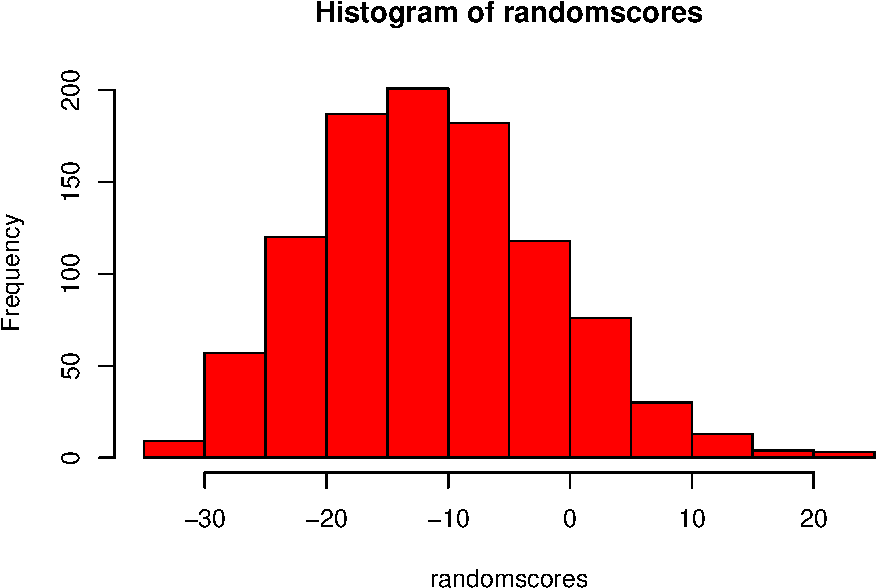
\includegraphics{lbrb_files/figure-latex/unnamed-chunk-349-1.pdf}

We can see from the histogram that quite a lot of the random sequences seem to have higher alignment scores than -5 when aligned to ``HEAGAWGHEE'' (where -5 is the alignment score for ``PAWHEAE'' and ``HEAGAWGHEE'').

We can use the vector randomscores of scores for 1000 alignments of random sequences to ``HEAGAWGHEE'' to calculate the probability of getting a score as large as the real alignment score for ``PAWHEAE'' and ``HEAGAWGHEE'' (i.e.~-5) by chance.

\begin{Shaded}
\begin{Highlighting}[]
\FunctionTok{sum}\NormalTok{(randomscores }\SpecialCharTok{\textgreater{}=} \SpecialCharTok{{-}}\DecValTok{5}\NormalTok{)}
\end{Highlighting}
\end{Shaded}

\begin{verbatim}
## [1] 274
\end{verbatim}

We see that 266 of the 1000 alignments of random sequences to ``HEAGAWGHEE'' had alignment scores that were equal to or greater than -5. Thus, we can estimate that the probability of getting a score as large as the real alignment score by chance is (266/1000 =) 0.266. In other words, we can calculate a P-value of 0.266. This probability or P-value is quite high (almost 30\%, or 1 in 3), so we can conclude that it is quite probable that we could get an alignment score as high as -5 by chance alone. This indicates that the sequences ``HEAGAWGHEE'' and ``PAWHEAE'' are not more similar than any two random sequences, and so they are probably not related sequences.

Another way of saying this is that the P-value that we calculated is high (0.266), and as a result we conclude that the alignment score for the sequences ``HEAGAWGHEE'' and ``PAWHEAE'' is not statistically significant. Generally, if the P-value that we calculate for an alignment of two sequences is \textgreater0.05, we conclude that the alignment score is not statistically significant, and that the sequences are probably not related. On the other hand, if the P-value is less than or equal to 0.05, we conclude that the alignment score is ``statistically significant'', and the sequences are very probably related (homologous).

\hypertarget{summary-3}{%
\section{Summary}\label{summary-3}}

In this practical, you will have learned to use the following functions:

\begin{itemize}
\tightlist
\item
  \texttt{data()} for reading in data that comes with an \emph{R} package
\item
  \texttt{double()} for creating a numeric vector for storing real (non-integer) numbers
\item
  \texttt{toupper()} for converting a string of characters from lowercase to uppercase
\end{itemize}

All of these functions belong to the standard installation of R.

You have also learned the following R functions that belong to bioinformatics packages:

\begin{itemize}
\tightlist
\item
  \texttt{nucleotideSubstitutionMatrix()} in the Biostrings package for making a nucleotide scoring matrix
\item
  \texttt{pairwiseAlignment()} in the Biostrings package for making a global alignment between two sequences
\item
  \texttt{c2s()} in the seqinr package for converting a sequence stored in a vector to a string of characters
\end{itemize}

\hypertarget{links-and-further-reading-1}{%
\section{Links and Further Reading}\label{links-and-further-reading-1}}

Some links are included here for further reading.

For background reading on sequence alignment, it is recommended to read Chapter 3 of Introduction to Computational Genomics: a case studies approach by Cristianini and Hahn (Cambridge University Press; www.computational-genomics.net/book/).

For more in-depth information and more examples on using the SeqinR package for sequence analysis, look at the SeqinR documentation, \url{http://pbil.univ-lyon1.fr/software/seqinr/doc.php?lang=eng}.

There is also a very nice chapter on ``Analyzing Sequences'', which includes examples of using SeqinR and Biostrings for sequence analysis, as well as details on how to implement algorithms such as Needleman-Wunsch and Smith-Waterman in R yourself, in the book Applied statistics for bioinformatics using R by Krijnen (available online at cran.r-project.org/doc/contrib/Krijnen-IntroBioInfStatistics.pdf).

For a more in-depth introduction to R, a good online tutorial is available on the ``Kickstarting R'' website, cran.r-project.org/doc/contrib/Lemon-kickstart.

There is another nice (slightly more in-depth) tutorial to R available on the ``Introduction to R'' website, cran.r-project.org/doc/manuals/R-intro.html.

For more information on and examples using the Biostrings package, see the Biostrings documentation at \url{http://www.bioconductor.org/packages/release/bioc/html/Biostrings.html}.

The examples of DNA sequences and protein sequences to align (`GAATTC' and `GATTA', and sequences ``PAWHEAE'' and ``HEAGAWGHEE''), as well as some ideas related to finding the statistical significance of a pairwise alignment, were inspired by the chapter on ``Analyzing Sequences'' in the book Applied statistics for bioinformatics using R by Krijnen (cran.r-project.org/doc/contrib/Krijnen-IntroBioInfStatistics.pdf).

\hypertarget{exercises-1}{%
\section{Exercises}\label{exercises-1}}

Answer the following questions using \emph{R}. For each question, please record your answer, and what you typed into R to get this answer.

Model answers to the exercises are given in Answers to the exercises on Sequence Alignment.

\begin{enumerate}
\def\labelenumi{\arabic{enumi}.}
\tightlist
\item
  Download FASTA-format files of the \textbf{Brugia malayi} Vab-3 protein (UniProt accession A8PZ80) and the \emph{Loa loa} Vab-3 protein (UniProt accession E1FTG0) sequences from UniProt.
  Note: the vab-3 gene of \emph{Brugia malayi} and the vab-3 gene of \emph{Loa loa} are related genes that control eye development in these two species. \emph{Brugia malayi} and \emph{Loa loa} are both parasitic nematode worms, which both cause filariasis, which is classified by the WHO as a neglected tropical disease.
\item
  What is the alignment score for the optimal global alignment between the \emph{Brugia malayi} Vab-3 protein and the \emph{Loa loa} Vab-3 protein, when you use the BLOSUM50 scoring matrix, a gap opening penalty of -10 and a gap extension penalty of -0.5?
  Note: to specify a gap opening penalty of -10 and a gap extension penalty of -0.5, set the \texttt{gapOpening} argument to -9.5, and the \texttt{gapExtension} penalty to -0.5 in the \texttt{pairwiseAlignment()} function.
\item
  Use the print\_pairwise\_alignment() function to view the optimal global alignment between \textbf{Brugia malayi} Vab-3 protein and the \emph{Loa loa} Vab-3 protein, using the BLOSUM50 scoring matrix, a gap opening penalty of -10 and a gap extension penalty of -0.5.
  Do you see any regions where the alignment is very good (lots of identities and few gaps)?
\item
  What global alignment score do you get for the two Vab-3 proteins, when you use the BLOSUM62 alignment matrix, a gap opening penalty of -10 and a gap extension penalty of -0.5?
  Which scoring matrix do you think is more appropriate for using for this pair of proteins: BLOSUM50 or BLOSUM62?
\item
  What is the statistical significance of the optimal global alignment for the \textbf{Brugia malayi} and \textbf{Loa loa} Vab-3 proteins made using the BLOSUM50 scoring matrix, with a gap opening penalty of -10 and a gap extension penalty of -0.5?
  In other words, what is the probability of getting a score as large as the real alignment score for Vab-3 by chance?
\item
  What is the optimal global alignment score between the \emph{Brugia malayi} Vab-6 protein and the \emph{Mycobacterium leprae} chorismate lyase protein?
  Is the alignment score statistically significant (what is the P- value?)? Does this surprise you?
\end{enumerate}

\hypertarget{retrieving-multiple-sequences-in-r}{%
\chapter{Retrieving multiple sequences in R}\label{retrieving-multiple-sequences-in-r}}

\begin{Shaded}
\begin{Highlighting}[]
\FunctionTok{library}\NormalTok{(compbio4all)}
\end{Highlighting}
\end{Shaded}

\textbf{By}: Avril Coghlan.\\
Multiple Alignment and Phylogenetic trees
\url{https://a-little-book-of-r-for-bioinformatics.readthedocs.io/en/latest/src/chapter5.html}

\textbf{Adapted, edited and expanded}: Nathan Brouwer under the Creative Commons 3.0 Attribution License \href{https://creativecommons.org/licenses/by/3.0/}{(CC BY 3.0)}.

\hypertarget{prelminaries}{%
\section{Prelminaries}\label{prelminaries}}

\begin{Shaded}
\begin{Highlighting}[]
\DocumentationTok{\#\# package}
\FunctionTok{library}\NormalTok{(compbio4all)}
\FunctionTok{library}\NormalTok{(rentrez)    }\CommentTok{\# still needed?}
\end{Highlighting}
\end{Shaded}

\hypertarget{retrieving-a-set-of-sequences-from-uniprot}{%
\section{Retrieving a set of sequences from UniProt}\label{retrieving-a-set-of-sequences-from-uniprot}}

Using websites or \emph{R} you can search fort DNA or protein sequences in sequence databases such as the \textbf{NCBI} database and \textbf{UniProt}. Oftentimes, it is useful to retrieve several sequences at once. The \emph{R} function \texttt{entrez\_fetch()} from the \emph{rentrez} package is useful for this purpose. Other packages can also, such as \texttt{sequinr} this but \emph{rentrez} has the cleanest interface.

We'll retrieve the protein sequences for these UniProt accessions

\begin{enumerate}
\def\labelenumi{\arabic{enumi}.}
\tightlist
\item
  P06747: rabies virus phosphoprotein
\item
  P0C569: Mokola virus phosphoprotein
\item
  O56773: Lagos bat virus phosphoprotein
\item
  Q5VKP1: Western Caucasian bat virus phosphoprotein
\end{enumerate}

Rabies virus is the virus responsible for rabies, which is classified by the WHO as a \textbf{neglected tropical disease}. Rabies is not a major human pathogen in the USA and Europe, but is problem in Africa. {[}Mokola virus{]}(\url{https://en.wikipedia.org/wiki/Mokola_lyssavirus}() and rabies virus are closely related viruses that both belong to a group of viruses called the \href{https://en.wikipedia.org/wiki/Lyssavirus}{Lyssaviruses}. Mokola virus causes a rabies-like infection in mammals including humans.

You can type make a vector containing the names of the sequences. Note that the accessions aren't numbers but are \textbf{quoted character strings}:

\begin{Shaded}
\begin{Highlighting}[]
\NormalTok{seqnames }\OtherTok{\textless{}{-}} \FunctionTok{c}\NormalTok{(}\StringTok{"P06747"}\NormalTok{, }
              \StringTok{"P0C569"}\NormalTok{, }
              \StringTok{"O56773"}\NormalTok{, }
              \StringTok{"Q5VKP1"}\NormalTok{)  }
\end{Highlighting}
\end{Shaded}

Confirm that we are working with character data using \texttt{is.character()}

\begin{Shaded}
\begin{Highlighting}[]
\FunctionTok{is.character}\NormalTok{(seqnames)}
\end{Highlighting}
\end{Shaded}

\begin{verbatim}
## [1] TRUE
\end{verbatim}

We can access the first element of the vector, P06747, using \textbf{bracket notation} like this:

\begin{Shaded}
\begin{Highlighting}[]
\NormalTok{seqnames[}\DecValTok{1}\NormalTok{]}
\end{Highlighting}
\end{Shaded}

\begin{verbatim}
## [1] "P06747"
\end{verbatim}

The code to access the second and third elements of the vector of accessions is:

\begin{Shaded}
\begin{Highlighting}[]
\CommentTok{\# 2nd accession}
\NormalTok{seqnames[}\DecValTok{2}\NormalTok{]}
\end{Highlighting}
\end{Shaded}

\begin{verbatim}
## [1] "P0C569"
\end{verbatim}

\begin{Shaded}
\begin{Highlighting}[]
\CommentTok{\# 3rd accession}
\NormalTok{seqnames[}\DecValTok{3}\NormalTok{]}
\end{Highlighting}
\end{Shaded}

\begin{verbatim}
## [1] "O56773"
\end{verbatim}

Now let's use this vector of accessions to download sequence data. To make sure we understand what we're doing, first we'll download just the sequences one by one. This code retrieves the first sequence and store them in vector variable \texttt{seqs}.

\begin{Shaded}
\begin{Highlighting}[]
\NormalTok{seq1 }\OtherTok{\textless{}{-}}\NormalTok{ rentrez}\SpecialCharTok{::}\FunctionTok{entrez\_fetch}\NormalTok{(}\AttributeTok{db =} \StringTok{"protein"}\NormalTok{, }
                          \AttributeTok{id =}\NormalTok{ seqnames[}\DecValTok{1}\NormalTok{], }
                          \AttributeTok{rettype =} \StringTok{"fasta"}\NormalTok{)      }
\end{Highlighting}
\end{Shaded}

We can do the next two sequences by change \texttt{id\ =\ ...} to \texttt{seqnames{[}2{]}} and \texttt{seqnames{[}3{]}}.

\begin{Shaded}
\begin{Highlighting}[]
\CommentTok{\# sequence two using seqnames[2]}
\NormalTok{seq2 }\OtherTok{\textless{}{-}}\NormalTok{ rentrez}\SpecialCharTok{::}\FunctionTok{entrez\_fetch}\NormalTok{(}\AttributeTok{db =} \StringTok{"protein"}\NormalTok{, }
                          \AttributeTok{id =}\NormalTok{ seqnames[}\DecValTok{2}\NormalTok{], }
                          \AttributeTok{rettype =} \StringTok{"fasta"}\NormalTok{) }

\CommentTok{\# sequence two using seqnames[3]}
\NormalTok{seq3 }\OtherTok{\textless{}{-}}\NormalTok{ rentrez}\SpecialCharTok{::}\FunctionTok{entrez\_fetch}\NormalTok{(}\AttributeTok{db =} \StringTok{"protein"}\NormalTok{, }
                          \AttributeTok{id =}\NormalTok{ seqnames[}\DecValTok{3}\NormalTok{], }
                          \AttributeTok{rettype =} \StringTok{"fasta"}\NormalTok{)}

\CommentTok{\# sequence two using seqnames[4]}
\NormalTok{seq4 }\OtherTok{\textless{}{-}}\NormalTok{ rentrez}\SpecialCharTok{::}\FunctionTok{entrez\_fetch}\NormalTok{(}\AttributeTok{db =} \StringTok{"protein"}\NormalTok{, }
                          \AttributeTok{id =}\NormalTok{ seqnames[}\DecValTok{4}\NormalTok{], }
                          \AttributeTok{rettype =} \StringTok{"fasta"}\NormalTok{)}
\end{Highlighting}
\end{Shaded}

Each of these is in raw FASTA format

\begin{Shaded}
\begin{Highlighting}[]
\NormalTok{seq1}
\end{Highlighting}
\end{Shaded}

\begin{verbatim}
## [1] ">sp|P06747.1|PHOSP_RABVP RecName: Full=Phosphoprotein; Short=Protein P; AltName: Full=Protein M1\nMSKIFVNPSAIRAGLADLEMAEETVDLINRNIEDNQAHLQGEPIEVDNLPEDMGRLHLDDGKSPNPGEMA\nKVGEGKYREDFQMDEGEDPSLLFQSYLDNVGVQIVRQIRSGERFLKIWSQTVEEIISYVAVNFPNPPGKS\nSEDKSTQTTGRELKKETTPTPSQRESQSSKARMAAQTASGPPALEWSATNEEDDLSVEAEIAHQIAESFS\nKKYKFPSRSSGILLYNFEQLKMNLDDIVKEAKNVPGVTRLARDGSKLPLRCVLGWVALANSKKFQLLVES\nNKLSKIMQDDLNRYTSC\n\n"
\end{verbatim}

To do an analysis of these we need to clean each of these vectors using \texttt{fasta\_cleaner()}.

\begin{Shaded}
\begin{Highlighting}[]
\NormalTok{seq1 }\OtherTok{\textless{}{-}} \FunctionTok{fasta\_cleaner}\NormalTok{(seq1, }\AttributeTok{parse =}\NormalTok{ T)  }
\NormalTok{seq2 }\OtherTok{\textless{}{-}} \FunctionTok{fasta\_cleaner}\NormalTok{(seq2, }\AttributeTok{parse =}\NormalTok{ T)  }
\NormalTok{seq3 }\OtherTok{\textless{}{-}} \FunctionTok{fasta\_cleaner}\NormalTok{(seq3, }\AttributeTok{parse =}\NormalTok{ T)  }
\NormalTok{seq4 }\OtherTok{\textless{}{-}} \FunctionTok{fasta\_cleaner}\NormalTok{(seq4, }\AttributeTok{parse =}\NormalTok{ T)  }
\end{Highlighting}
\end{Shaded}

Print out the first 20 letters of the first sequence

\begin{Shaded}
\begin{Highlighting}[]
\NormalTok{seq1[}\DecValTok{1}\SpecialCharTok{:}\DecValTok{20}\NormalTok{]                                   }
\end{Highlighting}
\end{Shaded}

\begin{verbatim}
##  [1] "M" "S" "K" "I" "F" "V" "N" "P" "S" "A" "I" "R" "A" "G" "L" "A" "D" "L" "E"
## [20] "M"
\end{verbatim}

Print out the first 20 letters of the second sequence

\begin{Shaded}
\begin{Highlighting}[]
\NormalTok{seq2[}\DecValTok{1}\SpecialCharTok{:}\DecValTok{20}\NormalTok{]                                   }
\end{Highlighting}
\end{Shaded}

\begin{verbatim}
##  [1] "M" "S" "K" "D" "L" "V" "H" "P" "S" "L" "I" "R" "A" "G" "I" "V" "E" "L" "E"
## [20] "M"
\end{verbatim}

We have these four sequences, each cleaned and in its own vector. We can therefore do dotplots, alignments, and other analyses. Creating all these separate vectors is a bit laborious. Luckily \texttt{entrez\_fetch()} can download multiple sequences for us.

\hypertarget{downloading-sequences-in-bulk}{%
\section{Downloading sequences in bulk}\label{downloading-sequences-in-bulk}}

Previously we were giving \texttt{entrez\_fetch} the name of just one sequence at a time by using square brackets on our \texttt{seqnames} vector, e.g.~\texttt{seqnames{[}1{]}}, \texttt{seqnames{[}2{]}} etc. If don't include square brackets, \texttt{entrez\_fetch()} will download \emph{all} of the sequences in succession and package them up into a single long, formatted string. This may take a second or two, depending on your internet connection and how busy the NCBI servers are.

\begin{Shaded}
\begin{Highlighting}[]
\NormalTok{seq\_1\_2\_3\_4 }\OtherTok{\textless{}{-}}\NormalTok{ rentrez}\SpecialCharTok{::}\FunctionTok{entrez\_fetch}\NormalTok{(}\AttributeTok{db =} \StringTok{"protein"}\NormalTok{, }
                          \AttributeTok{id =}\NormalTok{ seqnames, }
                          \AttributeTok{rettype =} \StringTok{"fasta"}\NormalTok{)}
\end{Highlighting}
\end{Shaded}

We can view what we have in a nice format using the \texttt{cat()} function.

\begin{Shaded}
\begin{Highlighting}[]
\FunctionTok{cat}\NormalTok{(seq\_1\_2\_3\_4)}
\end{Highlighting}
\end{Shaded}

\begin{verbatim}
## >sp|P06747.1|PHOSP_RABVP RecName: Full=Phosphoprotein; Short=Protein P; AltName: Full=Protein M1
## MSKIFVNPSAIRAGLADLEMAEETVDLINRNIEDNQAHLQGEPIEVDNLPEDMGRLHLDDGKSPNPGEMA
## KVGEGKYREDFQMDEGEDPSLLFQSYLDNVGVQIVRQIRSGERFLKIWSQTVEEIISYVAVNFPNPPGKS
## SEDKSTQTTGRELKKETTPTPSQRESQSSKARMAAQTASGPPALEWSATNEEDDLSVEAEIAHQIAESFS
## KKYKFPSRSSGILLYNFEQLKMNLDDIVKEAKNVPGVTRLARDGSKLPLRCVLGWVALANSKKFQLLVES
## NKLSKIMQDDLNRYTSC
## 
## >sp|P0C569.1|PHOSP_MOKV RecName: Full=Phosphoprotein; Short=Protein P; AltName: Full=Protein M1
## MSKDLVHPSLIRAGIVELEMAEETTDLINRTIESNQAHLQGEPLYVDSLPEDMSRLRIEDKSRRTKTEEE
## ERDEGSSEEDNYLSEGQDPLIPFQNFLDEIGARAVKRLKTGEGFFRVWSALSDDIKGYVSTNIMTSGERD
## TKSIQIQTEPTASVSSGNESRHDSESMHDPNDKKDHTPDHDVVPDIESSTDKGEIRDIEGEVAHQVAESF
## SKKYKFPSRSSGIFLWNFEQLKMNLDDIVKAAMNVPGVERIAEKGGKLPLRCILGFVALDSSKRFRLLAD
## NDKVARLIQEDINSYMARLEEAE
## 
## >sp|O56773.1|PHOSP_LBV RecName: Full=Phosphoprotein; Short=Protein P; AltName: Full=Protein M1
## MSKGLIHPSAIRSGLVDLEMAEETVDLVHKNLADSQAHLQGEPLNVDSLPEDMRKMRLTNAPSEREIIEE
## DEEEYSSEDEYYLSQGQDPMVPFQNFLDELGTQIVRRMKSGDGFFKIWSAASEDIKGYVLSTFMKPETQA
## TVSKPTQTDSLSVPRPSQGYTSVPRDKPSNSESQGGGVKPKKVQKSEWTRDTDEISDIEGEVAHQVAESF
## SKKYKFPSRSSGIFLWNFEQLKMNLDDIVKTSMNVPGVDKIAEKGGKLPLRCILGFVSLDSSKRFRLLAD
## TDKVARLMQDDIHNYMTRIEEIDHN
## 
## >sp|Q5VKP1.1|PHOSP_WCBV RecName: Full=Phosphoprotein; Short=Protein P; AltName: Full=Protein M1
## MSKSLIHPSDLRAGLADIEMADETVDLVYKNLSEGQAHLQGEPFDIKDLPEGVSKLQISDNVRSDTSPNE
## YSDEDDEEGEDEYEEVYDPVSAFQDFLDETGSYLISKLKKGEKIKKTWSEVSRVIYSYVMSNFPPRPPKP
## TTKDIAVQADLKKPNEIQKISEHKSKSEPSPREPVVEMHKHATLENPEDDEGALESEIAHQVAESYSKKY
## KFPSKSSGIFLWNFEQLKMNLDDIVQVARGVPGISQIVERGGKLPLRCMLGYVGLETSKRFRSLVNQDKL
## CKLMQEDLNAYSVSSNN
\end{verbatim}

This is a good way to store FASTA files, but we can't work with them in this format - they need to be in vectors. To give us FASTA data in a usable form the \texttt{compbio4all} package has a function called \texttt{entrez\_fetch\_list()}, which is a \textbf{wrapper} for \texttt{entrez\_fetch()} which returns each sequence in its own separate slot in a list.

\begin{Shaded}
\begin{Highlighting}[]
\NormalTok{seq\_1\_2\_3\_4 }\OtherTok{\textless{}{-}} \FunctionTok{entrez\_fetch\_list}\NormalTok{(}\AttributeTok{db =} \StringTok{"protein"}\NormalTok{, }
                          \AttributeTok{id =}\NormalTok{ seqnames, }
                          \AttributeTok{rettype =} \StringTok{"fasta"}\NormalTok{)}
\end{Highlighting}
\end{Shaded}

Let's look at the output

\begin{Shaded}
\begin{Highlighting}[]
\NormalTok{seq\_1\_2\_3\_4}
\end{Highlighting}
\end{Shaded}

\begin{verbatim}
## $P06747
## [1] ">sp|P06747.1|PHOSP_RABVP RecName: Full=Phosphoprotein; Short=Protein P; AltName: Full=Protein M1\nMSKIFVNPSAIRAGLADLEMAEETVDLINRNIEDNQAHLQGEPIEVDNLPEDMGRLHLDDGKSPNPGEMA\nKVGEGKYREDFQMDEGEDPSLLFQSYLDNVGVQIVRQIRSGERFLKIWSQTVEEIISYVAVNFPNPPGKS\nSEDKSTQTTGRELKKETTPTPSQRESQSSKARMAAQTASGPPALEWSATNEEDDLSVEAEIAHQIAESFS\nKKYKFPSRSSGILLYNFEQLKMNLDDIVKEAKNVPGVTRLARDGSKLPLRCVLGWVALANSKKFQLLVES\nNKLSKIMQDDLNRYTSC\n\n"
## 
## $P0C569
## [1] ">sp|P0C569.1|PHOSP_MOKV RecName: Full=Phosphoprotein; Short=Protein P; AltName: Full=Protein M1\nMSKDLVHPSLIRAGIVELEMAEETTDLINRTIESNQAHLQGEPLYVDSLPEDMSRLRIEDKSRRTKTEEE\nERDEGSSEEDNYLSEGQDPLIPFQNFLDEIGARAVKRLKTGEGFFRVWSALSDDIKGYVSTNIMTSGERD\nTKSIQIQTEPTASVSSGNESRHDSESMHDPNDKKDHTPDHDVVPDIESSTDKGEIRDIEGEVAHQVAESF\nSKKYKFPSRSSGIFLWNFEQLKMNLDDIVKAAMNVPGVERIAEKGGKLPLRCILGFVALDSSKRFRLLAD\nNDKVARLIQEDINSYMARLEEAE\n\n"
## 
## $O56773
## [1] ">sp|O56773.1|PHOSP_LBV RecName: Full=Phosphoprotein; Short=Protein P; AltName: Full=Protein M1\nMSKGLIHPSAIRSGLVDLEMAEETVDLVHKNLADSQAHLQGEPLNVDSLPEDMRKMRLTNAPSEREIIEE\nDEEEYSSEDEYYLSQGQDPMVPFQNFLDELGTQIVRRMKSGDGFFKIWSAASEDIKGYVLSTFMKPETQA\nTVSKPTQTDSLSVPRPSQGYTSVPRDKPSNSESQGGGVKPKKVQKSEWTRDTDEISDIEGEVAHQVAESF\nSKKYKFPSRSSGIFLWNFEQLKMNLDDIVKTSMNVPGVDKIAEKGGKLPLRCILGFVSLDSSKRFRLLAD\nTDKVARLMQDDIHNYMTRIEEIDHN\n\n"
## 
## $Q5VKP1
## [1] ">sp|Q5VKP1.1|PHOSP_WCBV RecName: Full=Phosphoprotein; Short=Protein P; AltName: Full=Protein M1\nMSKSLIHPSDLRAGLADIEMADETVDLVYKNLSEGQAHLQGEPFDIKDLPEGVSKLQISDNVRSDTSPNE\nYSDEDDEEGEDEYEEVYDPVSAFQDFLDETGSYLISKLKKGEKIKKTWSEVSRVIYSYVMSNFPPRPPKP\nTTKDIAVQADLKKPNEIQKISEHKSKSEPSPREPVVEMHKHATLENPEDDEGALESEIAHQVAESYSKKY\nKFPSKSSGIFLWNFEQLKMNLDDIVQVARGVPGISQIVERGGKLPLRCMLGYVGLETSKRFRSLVNQDKL\nCKLMQEDLNAYSVSSNN\n\n"
\end{verbatim}

Note that before each sequence is its name, preceded by a dollar sign, e.g.~\texttt{\$P06747}.

This is the name of each element of our list. We can confirm that we have a list using \texttt{is.list()}.

\begin{Shaded}
\begin{Highlighting}[]
\FunctionTok{is.list}\NormalTok{(seq\_1\_2\_3\_4)}
\end{Highlighting}
\end{Shaded}

\begin{verbatim}
## [1] TRUE
\end{verbatim}

The size of the list is the number of elements it contains, not the amount of data in each element. There are 4 sequences, so 4 elements, so length = 4.

\begin{Shaded}
\begin{Highlighting}[]
\FunctionTok{length}\NormalTok{(seq\_1\_2\_3\_4)}
\end{Highlighting}
\end{Shaded}

\begin{verbatim}
## [1] 4
\end{verbatim}

We can access each element of the list by name, like this:

\begin{Shaded}
\begin{Highlighting}[]
\NormalTok{seq\_1\_2\_3\_4}\SpecialCharTok{$}\NormalTok{P06747}
\end{Highlighting}
\end{Shaded}

\begin{verbatim}
## [1] ">sp|P06747.1|PHOSP_RABVP RecName: Full=Phosphoprotein; Short=Protein P; AltName: Full=Protein M1\nMSKIFVNPSAIRAGLADLEMAEETVDLINRNIEDNQAHLQGEPIEVDNLPEDMGRLHLDDGKSPNPGEMA\nKVGEGKYREDFQMDEGEDPSLLFQSYLDNVGVQIVRQIRSGERFLKIWSQTVEEIISYVAVNFPNPPGKS\nSEDKSTQTTGRELKKETTPTPSQRESQSSKARMAAQTASGPPALEWSATNEEDDLSVEAEIAHQIAESFS\nKKYKFPSRSSGILLYNFEQLKMNLDDIVKEAKNVPGVTRLARDGSKLPLRCVLGWVALANSKKFQLLVES\nNKLSKIMQDDLNRYTSC\n\n"
\end{verbatim}

We can also access it by its index number, like this, using \textbf{double-bracket notation.}

\begin{Shaded}
\begin{Highlighting}[]
\NormalTok{seq\_1\_2\_3\_4[[}\DecValTok{1}\NormalTok{]] }\CommentTok{\#NOTE: double brackets}
\end{Highlighting}
\end{Shaded}

\begin{verbatim}
## [1] ">sp|P06747.1|PHOSP_RABVP RecName: Full=Phosphoprotein; Short=Protein P; AltName: Full=Protein M1\nMSKIFVNPSAIRAGLADLEMAEETVDLINRNIEDNQAHLQGEPIEVDNLPEDMGRLHLDDGKSPNPGEMA\nKVGEGKYREDFQMDEGEDPSLLFQSYLDNVGVQIVRQIRSGERFLKIWSQTVEEIISYVAVNFPNPPGKS\nSEDKSTQTTGRELKKETTPTPSQRESQSSKARMAAQTASGPPALEWSATNEEDDLSVEAEIAHQIAESFS\nKKYKFPSRSSGILLYNFEQLKMNLDDIVKEAKNVPGVTRLARDGSKLPLRCVLGWVALANSKKFQLLVES\nNKLSKIMQDDLNRYTSC\n\n"
\end{verbatim}

Each element of the list is a vector. We can check this using \texttt{is.vector()} like this

\begin{Shaded}
\begin{Highlighting}[]
\FunctionTok{is.vector}\NormalTok{(seq\_1\_2\_3\_4}\SpecialCharTok{$}\NormalTok{P06747)}
\end{Highlighting}
\end{Shaded}

\begin{verbatim}
## [1] TRUE
\end{verbatim}

or using double brackets like this

\begin{Shaded}
\begin{Highlighting}[]
\FunctionTok{is.vector}\NormalTok{(seq\_1\_2\_3\_4[[}\DecValTok{1}\NormalTok{]])}
\end{Highlighting}
\end{Shaded}

Its character data, which we can confirm with \texttt{class()}

\begin{Shaded}
\begin{Highlighting}[]
\FunctionTok{class}\NormalTok{(seq\_1\_2\_3\_4}\SpecialCharTok{$}\NormalTok{P06747) }\CommentTok{\# dollar sign notation}
\FunctionTok{class}\NormalTok{(seq\_1\_2\_3\_4[[}\DecValTok{1}\NormalTok{]])   }\CommentTok{\# double{-}bracket notation}
\end{Highlighting}
\end{Shaded}

\hypertarget{manipulating-matrices-and-vectors-worked-example}{%
\chapter{Manipulating matrices and vectors: worked example}\label{manipulating-matrices-and-vectors-worked-example}}

\textbf{By} Nathan Brouwer

\hypertarget{introduction-2}{%
\section{Introduction}\label{introduction-2}}

In this exercise we will practice manipulating matrices and vectors by exploring the structure of \textbf{scoring matrices}.

\hypertarget{preliminaries-10}{%
\section{Preliminaries}\label{preliminaries-10}}

\hypertarget{packages-3}{%
\subsection{Packages}\label{packages-3}}

\begin{itemize}
\tightlist
\item
  BiocManager
\item
  Biostrings
\item
  combio4all
\end{itemize}

\hypertarget{vocab-2}{%
\subsection{Vocab}\label{vocab-2}}

\hypertarget{math-r-vocab-1}{%
\subsubsection{Math / R vocab}\label{math-r-vocab-1}}

\begin{itemize}
\tightlist
\item
  triangular matrix
\item
  square matrix
\item
  lower triangle
\item
  upper triangle
\item
  symmetric matrix
\item
  matrix diagonal
\item
  named vectors
\item
  named matrices
\item
  accessing items in named vectors or matrices
\item
  square bracket notation
\end{itemize}

\hypertarget{bioinformatics-vocab-1}{%
\subsubsection{Bioinformatics vocab}\label{bioinformatics-vocab-1}}

\begin{itemize}
\tightlist
\item
  scoring matrix
\item
  BLOSUM scoring matrix
\end{itemize}

\hypertarget{functions-used-1}{%
\subsection{Functions used}\label{functions-used-1}}

\hypertarget{base-r-functions-1}{%
\subsubsection{Base R functions}\label{base-r-functions-1}}

\begin{itemize}
\tightlist
\item
  \texttt{data()}
\item
  \texttt{is()}
\item
  \texttt{nrow()}, \texttt{ncol()},
\item
  \texttt{dim()},
\item
  \texttt{names()}, \texttt{colnames()}, \texttt{rownames()},
\item
  \texttt{head()}, \texttt{tail()}
\end{itemize}

\hypertarget{packages-4}{%
\subsection{Packages}\label{packages-4}}

\begin{Shaded}
\begin{Highlighting}[]
\FunctionTok{library}\NormalTok{(Biostrings)}
\end{Highlighting}
\end{Shaded}

\hypertarget{data-2}{%
\subsection{Data}\label{data-2}}

\begin{Shaded}
\begin{Highlighting}[]
\FunctionTok{data}\NormalTok{(BLOSUM62)}
\end{Highlighting}
\end{Shaded}

\hypertarget{matrix-elements-can-be-accessed-with-square-bracket-notation}{%
\section{Matrix elements can be accessed with square bracket notation}\label{matrix-elements-can-be-accessed-with-square-bracket-notation}}

We often want to access just subsets of data from a matrix or a dataframe. This can take some getting used to. We can use \textbf{square brackets} to get certain subsets or ranges of cells. If we want just the upper left-hand cell we can do this:

\begin{Shaded}
\begin{Highlighting}[]
\NormalTok{BLOSUM62[}\DecValTok{1}\NormalTok{,}\DecValTok{1}\NormalTok{]}
\end{Highlighting}
\end{Shaded}

\begin{verbatim}
## [1] 4
\end{verbatim}

If we want the first four cells in the upper left hand corner we can do this

\begin{Shaded}
\begin{Highlighting}[]
\NormalTok{BLOSUM62[}\FunctionTok{c}\NormalTok{(}\DecValTok{1}\SpecialCharTok{:}\DecValTok{4}\NormalTok{), }\FunctionTok{c}\NormalTok{(}\DecValTok{1}\SpecialCharTok{:}\DecValTok{4}\NormalTok{)]}
\end{Highlighting}
\end{Shaded}

\begin{verbatim}
##    A  R  N  D
## A  4 -1 -2 -2
## R -1  5  0 -2
## N -2  0  6  1
## D -2 -2  1  6
\end{verbatim}

If we want to get rid of the \textbf{ambiguity code} cells on the bottom which are \texttt{B}, \texttt{J}, \texttt{Z}, \texttt{X} and \texttt{*} we can specify that we want elements 1 through 20. Let me step through this.

First, run the code below; what happens?

\begin{Shaded}
\begin{Highlighting}[]
\DecValTok{1}\SpecialCharTok{:}\DecValTok{4}
\end{Highlighting}
\end{Shaded}

\begin{verbatim}
## [1] 1 2 3 4
\end{verbatim}

Now do the same thing for 1 to 20:

Note that this next line should provide the same result as what you just did.

\begin{Shaded}
\begin{Highlighting}[]
\FunctionTok{c}\NormalTok{(}\DecValTok{1}\SpecialCharTok{:}\DecValTok{20}\NormalTok{)}
\end{Highlighting}
\end{Shaded}

\begin{verbatim}
##  [1]  1  2  3  4  5  6  7  8  9 10 11 12 13 14 15 16 17 18 19 20
\end{verbatim}

If we \emph{really} wanted to type all of this out, we would have to do this:

\begin{Shaded}
\begin{Highlighting}[]
\FunctionTok{c}\NormalTok{(}\DecValTok{1}\NormalTok{,}\DecValTok{2}\NormalTok{,}\DecValTok{3}\NormalTok{,}\DecValTok{4}\NormalTok{,}\DecValTok{5}\NormalTok{,}\DecValTok{6}\NormalTok{,}\DecValTok{7}\NormalTok{,}\DecValTok{8}\NormalTok{,}\DecValTok{9}\NormalTok{,}\DecValTok{10}\NormalTok{,}\DecValTok{11}\NormalTok{,}\DecValTok{12}\NormalTok{,}\DecValTok{13}\NormalTok{,}\DecValTok{14}\NormalTok{,}\DecValTok{15}\NormalTok{,}\DecValTok{16}\NormalTok{,}\DecValTok{17}\NormalTok{,}\DecValTok{18}\NormalTok{,}\DecValTok{19}\NormalTok{,}\DecValTok{20}\NormalTok{)}
\end{Highlighting}
\end{Shaded}

\begin{verbatim}
##  [1]  1  2  3  4  5  6  7  8  9 10 11 12 13 14 15 16 17 18 19 20
\end{verbatim}

We can get just the first row of the BLOSUM matrix by telling \emph{R} we want row 1 and columns 1 to 20.

We get just \emph{row} 1 like this:

\begin{Shaded}
\begin{Highlighting}[]
\NormalTok{BLOSUM62[}\DecValTok{1}\NormalTok{, ]}
\end{Highlighting}
\end{Shaded}

\begin{verbatim}
##  A  R  N  D  C  Q  E  G  H  I  L  K  M  F  P  S  T  W  Y  V  B  J  Z  X  * 
##  4 -1 -2 -2  0 -1 -1  0 -2 -1 -1 -1 -1 -2 -1  1  0 -3 -2  0 -2 -1 -1 -1 -4
\end{verbatim}

We get columns 1:20 like this:

\begin{Shaded}
\begin{Highlighting}[]
\NormalTok{BLOSUM62[ , }\FunctionTok{c}\NormalTok{(}\DecValTok{1}\SpecialCharTok{:}\DecValTok{20}\NormalTok{)]}
\end{Highlighting}
\end{Shaded}

\begin{verbatim}
##    A  R  N  D  C  Q  E  G  H  I  L  K  M  F  P  S  T  W  Y  V
## A  4 -1 -2 -2  0 -1 -1  0 -2 -1 -1 -1 -1 -2 -1  1  0 -3 -2  0
## R -1  5  0 -2 -3  1  0 -2  0 -3 -2  2 -1 -3 -2 -1 -1 -3 -2 -3
## N -2  0  6  1 -3  0  0  0  1 -3 -3  0 -2 -3 -2  1  0 -4 -2 -3
## D -2 -2  1  6 -3  0  2 -1 -1 -3 -4 -1 -3 -3 -1  0 -1 -4 -3 -3
## C  0 -3 -3 -3  9 -3 -4 -3 -3 -1 -1 -3 -1 -2 -3 -1 -1 -2 -2 -1
## Q -1  1  0  0 -3  5  2 -2  0 -3 -2  1  0 -3 -1  0 -1 -2 -1 -2
## E -1  0  0  2 -4  2  5 -2  0 -3 -3  1 -2 -3 -1  0 -1 -3 -2 -2
## G  0 -2  0 -1 -3 -2 -2  6 -2 -4 -4 -2 -3 -3 -2  0 -2 -2 -3 -3
## H -2  0  1 -1 -3  0  0 -2  8 -3 -3 -1 -2 -1 -2 -1 -2 -2  2 -3
## I -1 -3 -3 -3 -1 -3 -3 -4 -3  4  2 -3  1  0 -3 -2 -1 -3 -1  3
## L -1 -2 -3 -4 -1 -2 -3 -4 -3  2  4 -2  2  0 -3 -2 -1 -2 -1  1
## K -1  2  0 -1 -3  1  1 -2 -1 -3 -2  5 -1 -3 -1  0 -1 -3 -2 -2
## M -1 -1 -2 -3 -1  0 -2 -3 -2  1  2 -1  5  0 -2 -1 -1 -1 -1  1
## F -2 -3 -3 -3 -2 -3 -3 -3 -1  0  0 -3  0  6 -4 -2 -2  1  3 -1
## P -1 -2 -2 -1 -3 -1 -1 -2 -2 -3 -3 -1 -2 -4  7 -1 -1 -4 -3 -2
## S  1 -1  1  0 -1  0  0  0 -1 -2 -2  0 -1 -2 -1  4  1 -3 -2 -2
## T  0 -1  0 -1 -1 -1 -1 -2 -2 -1 -1 -1 -1 -2 -1  1  5 -2 -2  0
## W -3 -3 -4 -4 -2 -2 -3 -2 -2 -3 -2 -3 -1  1 -4 -3 -2 11  2 -3
## Y -2 -2 -2 -3 -2 -1 -2 -3  2 -1 -1 -2 -1  3 -3 -2 -2  2  7 -1
## V  0 -3 -3 -3 -1 -2 -2 -3 -3  3  1 -2  1 -1 -2 -2  0 -3 -1  4
## B -2 -1  4  4 -3  0  1 -1  0 -3 -4  0 -3 -3 -2  0 -1 -4 -3 -3
## J -1 -2 -3 -3 -1 -2 -3 -4 -3  3  3 -3  2  0 -3 -2 -1 -2 -1  2
## Z -1  0  0  1 -3  4  4 -2  0 -3 -3  1 -1 -3 -1  0 -1 -2 -2 -2
## X -1 -1 -1 -1 -1 -1 -1 -1 -1 -1 -1 -1 -1 -1 -1 -1 -1 -1 -1 -1
## * -4 -4 -4 -4 -4 -4 -4 -4 -4 -4 -4 -4 -4 -4 -4 -4 -4 -4 -4 -4
\end{verbatim}

Note that leaving the first part blank gives us ALL the rows.

If we want just the first row AND the first 20 columns, we do this:

\begin{Shaded}
\begin{Highlighting}[]
\NormalTok{BLOSUM62[}\DecValTok{1}\NormalTok{ , }\FunctionTok{c}\NormalTok{(}\DecValTok{1}\SpecialCharTok{:}\DecValTok{20}\NormalTok{)]}
\end{Highlighting}
\end{Shaded}

\begin{verbatim}
##  A  R  N  D  C  Q  E  G  H  I  L  K  M  F  P  S  T  W  Y  V 
##  4 -1 -2 -2  0 -1 -1  0 -2 -1 -1 -1 -1 -2 -1  1  0 -3 -2  0
\end{verbatim}

Assign the output of the code \texttt{c(1:20)} to an object called \texttt{i} using the assignment operator \texttt{\textless{}-}. The code should like like this \texttt{i\ \textless{}-\ c(1:20)}.

\begin{Shaded}
\begin{Highlighting}[]
\NormalTok{i }\OtherTok{\textless{}{-}} \FunctionTok{c}\NormalTok{(}\DecValTok{1}\SpecialCharTok{:}\DecValTok{20}\NormalTok{)}
\end{Highlighting}
\end{Shaded}

This thing \texttt{i} we just made is a \textbf{vector} of numbers. Vectors are a 1-dimensional sequence of numbers. You can think of a matrix as a bunch of vectors stacked on top of each other.

Unfortunately, if you call \texttt{is()} in the \texttt{i} object you don't get a totally clear picture of what it is. Where does the word \texttt{vector} show up?

I'm not sure why \texttt{vector} isn't the first thing to be printed. We can check whether \texttt{i} is a vector more directly by asking it ``hey i, are you a vector'' using the \texttt{is.vector()} command

\begin{Shaded}
\begin{Highlighting}[]
\FunctionTok{is.vector}\NormalTok{(i)}
\end{Highlighting}
\end{Shaded}

\begin{verbatim}
## [1] TRUE
\end{verbatim}

Its a vector, so it shouldn't be a matrix, but we can check with \texttt{is.matrix()}

\begin{Shaded}
\begin{Highlighting}[]
\FunctionTok{is.matrix}\NormalTok{(i)}
\end{Highlighting}
\end{Shaded}

\begin{verbatim}
## [1] FALSE
\end{verbatim}

Math books may tell you that a vector is a 1-dimensional matrix, but in \emph{R} land vectors are distinct from matrices.

Vectors show up \emph{everywhere} in R. In this case I've defined a vector, \texttt{i}, which is holding the row and column numbers I want to isolated from the BLOSUM62 matrix.

I can call up just these rows and columns like this

\begin{Shaded}
\begin{Highlighting}[]
\NormalTok{BLOSUM62[i , i]}
\end{Highlighting}
\end{Shaded}

\begin{verbatim}
##    A  R  N  D  C  Q  E  G  H  I  L  K  M  F  P  S  T  W  Y  V
## A  4 -1 -2 -2  0 -1 -1  0 -2 -1 -1 -1 -1 -2 -1  1  0 -3 -2  0
## R -1  5  0 -2 -3  1  0 -2  0 -3 -2  2 -1 -3 -2 -1 -1 -3 -2 -3
## N -2  0  6  1 -3  0  0  0  1 -3 -3  0 -2 -3 -2  1  0 -4 -2 -3
## D -2 -2  1  6 -3  0  2 -1 -1 -3 -4 -1 -3 -3 -1  0 -1 -4 -3 -3
## C  0 -3 -3 -3  9 -3 -4 -3 -3 -1 -1 -3 -1 -2 -3 -1 -1 -2 -2 -1
## Q -1  1  0  0 -3  5  2 -2  0 -3 -2  1  0 -3 -1  0 -1 -2 -1 -2
## E -1  0  0  2 -4  2  5 -2  0 -3 -3  1 -2 -3 -1  0 -1 -3 -2 -2
## G  0 -2  0 -1 -3 -2 -2  6 -2 -4 -4 -2 -3 -3 -2  0 -2 -2 -3 -3
## H -2  0  1 -1 -3  0  0 -2  8 -3 -3 -1 -2 -1 -2 -1 -2 -2  2 -3
## I -1 -3 -3 -3 -1 -3 -3 -4 -3  4  2 -3  1  0 -3 -2 -1 -3 -1  3
## L -1 -2 -3 -4 -1 -2 -3 -4 -3  2  4 -2  2  0 -3 -2 -1 -2 -1  1
## K -1  2  0 -1 -3  1  1 -2 -1 -3 -2  5 -1 -3 -1  0 -1 -3 -2 -2
## M -1 -1 -2 -3 -1  0 -2 -3 -2  1  2 -1  5  0 -2 -1 -1 -1 -1  1
## F -2 -3 -3 -3 -2 -3 -3 -3 -1  0  0 -3  0  6 -4 -2 -2  1  3 -1
## P -1 -2 -2 -1 -3 -1 -1 -2 -2 -3 -3 -1 -2 -4  7 -1 -1 -4 -3 -2
## S  1 -1  1  0 -1  0  0  0 -1 -2 -2  0 -1 -2 -1  4  1 -3 -2 -2
## T  0 -1  0 -1 -1 -1 -1 -2 -2 -1 -1 -1 -1 -2 -1  1  5 -2 -2  0
## W -3 -3 -4 -4 -2 -2 -3 -2 -2 -3 -2 -3 -1  1 -4 -3 -2 11  2 -3
## Y -2 -2 -2 -3 -2 -1 -2 -3  2 -1 -1 -2 -1  3 -3 -2 -2  2  7 -1
## V  0 -3 -3 -3 -1 -2 -2 -3 -3  3  1 -2  1 -1 -2 -2  0 -3 -1  4
\end{verbatim}

If I hadn't defined the vector \texttt{i}, I could write

\begin{Shaded}
\begin{Highlighting}[]
\NormalTok{BLOSUM62[}\FunctionTok{c}\NormalTok{(}\DecValTok{1}\SpecialCharTok{:}\DecValTok{20}\NormalTok{) ,}\FunctionTok{c}\NormalTok{(}\DecValTok{1}\SpecialCharTok{:}\DecValTok{20}\NormalTok{)  ]}
\end{Highlighting}
\end{Shaded}

\begin{verbatim}
##    A  R  N  D  C  Q  E  G  H  I  L  K  M  F  P  S  T  W  Y  V
## A  4 -1 -2 -2  0 -1 -1  0 -2 -1 -1 -1 -1 -2 -1  1  0 -3 -2  0
## R -1  5  0 -2 -3  1  0 -2  0 -3 -2  2 -1 -3 -2 -1 -1 -3 -2 -3
## N -2  0  6  1 -3  0  0  0  1 -3 -3  0 -2 -3 -2  1  0 -4 -2 -3
## D -2 -2  1  6 -3  0  2 -1 -1 -3 -4 -1 -3 -3 -1  0 -1 -4 -3 -3
## C  0 -3 -3 -3  9 -3 -4 -3 -3 -1 -1 -3 -1 -2 -3 -1 -1 -2 -2 -1
## Q -1  1  0  0 -3  5  2 -2  0 -3 -2  1  0 -3 -1  0 -1 -2 -1 -2
## E -1  0  0  2 -4  2  5 -2  0 -3 -3  1 -2 -3 -1  0 -1 -3 -2 -2
## G  0 -2  0 -1 -3 -2 -2  6 -2 -4 -4 -2 -3 -3 -2  0 -2 -2 -3 -3
## H -2  0  1 -1 -3  0  0 -2  8 -3 -3 -1 -2 -1 -2 -1 -2 -2  2 -3
## I -1 -3 -3 -3 -1 -3 -3 -4 -3  4  2 -3  1  0 -3 -2 -1 -3 -1  3
## L -1 -2 -3 -4 -1 -2 -3 -4 -3  2  4 -2  2  0 -3 -2 -1 -2 -1  1
## K -1  2  0 -1 -3  1  1 -2 -1 -3 -2  5 -1 -3 -1  0 -1 -3 -2 -2
## M -1 -1 -2 -3 -1  0 -2 -3 -2  1  2 -1  5  0 -2 -1 -1 -1 -1  1
## F -2 -3 -3 -3 -2 -3 -3 -3 -1  0  0 -3  0  6 -4 -2 -2  1  3 -1
## P -1 -2 -2 -1 -3 -1 -1 -2 -2 -3 -3 -1 -2 -4  7 -1 -1 -4 -3 -2
## S  1 -1  1  0 -1  0  0  0 -1 -2 -2  0 -1 -2 -1  4  1 -3 -2 -2
## T  0 -1  0 -1 -1 -1 -1 -2 -2 -1 -1 -1 -1 -2 -1  1  5 -2 -2  0
## W -3 -3 -4 -4 -2 -2 -3 -2 -2 -3 -2 -3 -1  1 -4 -3 -2 11  2 -3
## Y -2 -2 -2 -3 -2 -1 -2 -3  2 -1 -1 -2 -1  3 -3 -2 -2  2  7 -1
## V  0 -3 -3 -3 -1 -2 -2 -3 -3  3  1 -2  1 -1 -2 -2  0 -3 -1  4
\end{verbatim}

Let's isolate just the first 20 rows and columns and put them into a new object called \texttt{BLOSUM62.subset}.

\begin{Shaded}
\begin{Highlighting}[]
\NormalTok{BLOSUM62.subset }\OtherTok{\textless{}{-}}\NormalTok{  BLOSUM62[i ,i ]}
\end{Highlighting}
\end{Shaded}

We can get the scores for when there is no change in an amino acid from the diagonal with \texttt{diag()}

\begin{Shaded}
\begin{Highlighting}[]
\FunctionTok{diag}\NormalTok{(BLOSUM62.subset)}
\end{Highlighting}
\end{Shaded}

\begin{verbatim}
##  A  R  N  D  C  Q  E  G  H  I  L  K  M  F  P  S  T  W  Y  V 
##  4  5  6  6  9  5  5  6  8  4  4  5  5  6  7  4  5 11  7  4
\end{verbatim}

If you're scoring an alignment by hand you can pull up the diagonal of the matrix this way so you don't have to squint at the whole matrix. We can make it even easier if we alphabetize thing, though this requires some extra code which you don't need to worry about. (I'm making a new vector, \texttt{i2}, which will do the alphabetizing).

\begin{Shaded}
\begin{Highlighting}[]
\CommentTok{\# get column names}
\NormalTok{n }\OtherTok{\textless{}{-}} \FunctionTok{colnames}\NormalTok{(BLOSUM62.subset)}

\CommentTok{\# sort}
\NormalTok{i2 }\OtherTok{\textless{}{-}} \FunctionTok{sort}\NormalTok{(n)}
\end{Highlighting}
\end{Shaded}

Now things are in alphabetical order

\begin{Shaded}
\begin{Highlighting}[]
\FunctionTok{diag}\NormalTok{(BLOSUM62.subset)[i2]}
\end{Highlighting}
\end{Shaded}

\begin{verbatim}
##  A  C  D  E  F  G  H  I  K  L  M  N  P  Q  R  S  T  V  W  Y 
##  4  9  6  5  6  6  8  4  5  4  5  6  7  5  5  4  5  4 11  7
\end{verbatim}

Save this alphabetized diagonal to an \texttt{R} object called \texttt{BLOSUM62.diag} using the assignment operator \texttt{\textless{}-}

\begin{Shaded}
\begin{Highlighting}[]
\NormalTok{BLOSUM62.diag }\OtherTok{\textless{}{-}} \FunctionTok{diag}\NormalTok{(BLOSUM62.subset)[i2]}
\end{Highlighting}
\end{Shaded}

What are the names attached to this \texttt{BLOSUM62.diag} object? Unfortunately \emph{R} is picky about how you do this so you need to figure out whether the functions \texttt{names()}, \texttt{rownames()}, or \texttt{colnames()} gets you want you want

\begin{Shaded}
\begin{Highlighting}[]
\FunctionTok{rownames}\NormalTok{(BLOSUM62.diag)}
\end{Highlighting}
\end{Shaded}

\begin{verbatim}
## NULL
\end{verbatim}

\begin{Shaded}
\begin{Highlighting}[]
\FunctionTok{colnames}\NormalTok{(BLOSUM62.diag)}
\end{Highlighting}
\end{Shaded}

\begin{verbatim}
## NULL
\end{verbatim}

\begin{Shaded}
\begin{Highlighting}[]
\FunctionTok{names}\NormalTok{(BLOSUM62.diag)}
\end{Highlighting}
\end{Shaded}

\begin{verbatim}
##  [1] "A" "C" "D" "E" "F" "G" "H" "I" "K" "L" "M" "N" "P" "Q" "R" "S" "T" "V" "W"
## [20] "Y"
\end{verbatim}

\hypertarget{r-object-names}{%
\section{R object names}\label{r-object-names}}

When an \emph{R} object has ``names'' assigned to it we can use the name to call up elements of the object.

\hypertarget{accessing-items-in-names-vectors}{%
\subsection{Accessing items in names vectors}\label{accessing-items-in-names-vectors}}

We can call up just the score for an E to E transition stored in our matrix diagonal like this, which is a way of saying ``Hey R, give me the value in this \texttt{BLOSUM62.diag} object that is in the slot labeled''E''.

\begin{Shaded}
\begin{Highlighting}[]
\NormalTok{BLOSUM62.diag[}\StringTok{"E"}\NormalTok{]}
\end{Highlighting}
\end{Shaded}

\begin{verbatim}
## E 
## 5
\end{verbatim}

E is the 4th slot so we can also get this value like this with the slot number.

\begin{Shaded}
\begin{Highlighting}[]
\NormalTok{BLOSUM62.diag[}\DecValTok{4}\NormalTok{]}
\end{Highlighting}
\end{Shaded}

\begin{verbatim}
## E 
## 5
\end{verbatim}

We could get the first four values using \texttt{c(1:4)}. Try it

What type of object is this diagonal thingy anyway? The command starts with ``i''.

\hypertarget{accessing-items-in-names-matrices}{%
\subsection{Accessing items in names matrices}\label{accessing-items-in-names-matrices}}

If we want to get something from the main matrix (the full BLOSUM matrix, not the diagonal) we can also specify things using the row and column names. This will give us the value for an E to E transition:

\begin{Shaded}
\begin{Highlighting}[]
\NormalTok{BLOSUM62.subset[}\StringTok{"E"}\NormalTok{,}\StringTok{"E"}\NormalTok{]}
\end{Highlighting}
\end{Shaded}

\begin{verbatim}
## [1] 5
\end{verbatim}

How could you get the whole ``E'' \emph{column}?

How could you get the whole ``E'' \emph{row}?

We can use numbers too if we want. ``E'' is in the 7th column, so we can get the E to E value like this:

\begin{Shaded}
\begin{Highlighting}[]
\NormalTok{BLOSUM62.subset[}\DecValTok{7}\NormalTok{,}\DecValTok{7}\NormalTok{]}
\end{Highlighting}
\end{Shaded}

\begin{verbatim}
## [1] 5
\end{verbatim}

How would you get the whole ``E'' column?

How would you get the whole ``E'' row?

\begin{Shaded}
\begin{Highlighting}[]
\NormalTok{BLOSUM62.subset[}\DecValTok{7}\NormalTok{, ]}
\end{Highlighting}
\end{Shaded}

\begin{verbatim}
##  A  R  N  D  C  Q  E  G  H  I  L  K  M  F  P  S  T  W  Y  V 
## -1  0  0  2 -4  2  5 -2  0 -3 -3  1 -2 -3 -1  0 -1 -3 -2 -2
\end{verbatim}

We can of course specify any score we want. For a P to A transition we could do this:

\begin{Shaded}
\begin{Highlighting}[]
\NormalTok{BLOSUM62.subset[}\StringTok{"P"}\NormalTok{,}\StringTok{"A"}\NormalTok{]}
\end{Highlighting}
\end{Shaded}

\begin{verbatim}
## [1] -1
\end{verbatim}

Or specify the row and column numbers

\begin{Shaded}
\begin{Highlighting}[]
\NormalTok{BLOSUM62.subset[}\DecValTok{15}\NormalTok{,}\DecValTok{1}\NormalTok{]}
\end{Highlighting}
\end{Shaded}

\begin{verbatim}
## [1] -1
\end{verbatim}

What happens when you do {[}``A'',``P''{]} instead (reverse of what was above?

So, if you are doing an alignment by hand, you can quickly query the matrix and pull up the scores. If you have a sequence ``EPEERPEWRDRPGSP'' and ``EAEREASWSEDRPGT'' you can get the score for the E to E matching again like this

\begin{Shaded}
\begin{Highlighting}[]
\NormalTok{BLOSUM62.subset[}\StringTok{"E"}\NormalTok{,}\StringTok{"E"}\NormalTok{]}
\end{Highlighting}
\end{Shaded}

\begin{verbatim}
## [1] 5
\end{verbatim}

and P to A like this

\begin{Shaded}
\begin{Highlighting}[]
\NormalTok{BLOSUM62.subset[}\StringTok{"P"}\NormalTok{,}\StringTok{"A"}\NormalTok{]}
\end{Highlighting}
\end{Shaded}

\begin{verbatim}
## [1] -1
\end{verbatim}

and so on.

\hypertarget{multiple-sequence-alignment-in-r}{%
\chapter{Multiple sequence alignment in R}\label{multiple-sequence-alignment-in-r}}

\textbf{By}: Nathan Brouwer, with some content adapted Coghlan (2011) \href{https://a-little-book-of-r-for-bioinformatics.readthedocs.io/en/latest/src/chapter5.html}{Multiple Alignment and Phylogenetic trees} and under the Creative Commons 3.0 Attribution License \href{https://creativecommons.org/licenses/by/3.0/}{(CC BY 3.0)}. Functions print\_msa() and clean\_alignment() adapted from (\href{https://a-little-book-of-r-for-bioinformatics.readthedocs.io/en/latest/\#}{Coglan 2011}).

\hypertarget{preliminaries-11}{%
\section{Preliminaries}\label{preliminaries-11}}

\hypertarget{packages-5}{%
\subsection{Packages}\label{packages-5}}

We'll be using the package \texttt{ggmsa} for the first time and you will have to install it using \texttt{install.packages("ggmsa")}. You may be asked to re-restart R more then once during the installation process.

\begin{Shaded}
\begin{Highlighting}[]
\CommentTok{\# new packages}
\DocumentationTok{\#\# Only install once}
\CommentTok{\# install.packages("ggmsa")}
\FunctionTok{library}\NormalTok{(ggmsa)       }\CommentTok{\# visualize MSA}

\CommentTok{\# other packages}
\FunctionTok{library}\NormalTok{(compbio4all)}
\FunctionTok{library}\NormalTok{(Biostrings)  }\CommentTok{\# convert FASTA to AAStringSet}
\FunctionTok{library}\NormalTok{(msa)         }\CommentTok{\# multiple sequence alignment}
\end{Highlighting}
\end{Shaded}

\hypertarget{functions-3}{%
\subsection{Functions}\label{functions-3}}

The following key functions from compbio4all are used in this lesson

\begin{itemize}
\tightlist
\item
  fasta\_cleaner()
\item
  entrez\_fetch\_list()
\item
  print\_msa()
\item
  clean\_alignment()
\end{itemize}

\hypertarget{multiple-sequence-alignment-msa}{%
\section{Multiple sequence alignment (MSA)}\label{multiple-sequence-alignment-msa}}

A common task in bioinformatics is to download a set of related sequences from a database, and then to align those sequences using multiple alignment software. This is the first step in almost all phylogenetic analyses using sequence data.

\hypertarget{make-msa-with-msa}{%
\section{Make MSA with msa()}\label{make-msa-with-msa}}

WE'll use a package called \texttt{msa} (\href{https://academic.oup.com/bioinformatics/article/31/24/3997/197486}{Bodenhofer et al.~2015}). There are several packages that can do multiple sequence alignment in R, but they all require loading an external piece of alignment software that is just accessed via R. The \texttt{msa} package actually runs the alignment algorithms entirely in R, making workflows simpler.

\hypertarget{data-preparation}{%
\subsection{Data preparation}\label{data-preparation}}

The data is stored in object in combio4all

\begin{Shaded}
\begin{Highlighting}[]
\FunctionTok{data}\NormalTok{(seq\_1\_2\_3\_4) }
\end{Highlighting}
\end{Shaded}

This data is in the form of a list

\begin{Shaded}
\begin{Highlighting}[]
\FunctionTok{is.list}\NormalTok{(seq\_1\_2\_3\_4)}
\end{Highlighting}
\end{Shaded}

\begin{verbatim}
## [1] TRUE
\end{verbatim}

First we need to clean each one using \texttt{fasta\_cleaner()}.

\begin{Shaded}
\begin{Highlighting}[]
\NormalTok{seq\_1\_2\_3\_4[[}\DecValTok{1}\NormalTok{]] }\OtherTok{\textless{}{-}} \FunctionTok{fasta\_cleaner}\NormalTok{(seq\_1\_2\_3\_4[[}\DecValTok{1}\NormalTok{]])}
\NormalTok{seq\_1\_2\_3\_4[[}\DecValTok{2}\NormalTok{]] }\OtherTok{\textless{}{-}} \FunctionTok{fasta\_cleaner}\NormalTok{(seq\_1\_2\_3\_4[[}\DecValTok{2}\NormalTok{]])}
\NormalTok{seq\_1\_2\_3\_4[[}\DecValTok{3}\NormalTok{]] }\OtherTok{\textless{}{-}} \FunctionTok{fasta\_cleaner}\NormalTok{(seq\_1\_2\_3\_4[[}\DecValTok{3}\NormalTok{]])}
\NormalTok{seq\_1\_2\_3\_4[[}\DecValTok{4}\NormalTok{]] }\OtherTok{\textless{}{-}} \FunctionTok{fasta\_cleaner}\NormalTok{(seq\_1\_2\_3\_4[[}\DecValTok{4}\NormalTok{]])}
\end{Highlighting}
\end{Shaded}

We need to put it into the form of a vector; in particular a \textbf{named vector}.

\begin{Shaded}
\begin{Highlighting}[]
\NormalTok{seq\_1\_2\_3\_4\_vector }\OtherTok{\textless{}{-}} \FunctionTok{c}\NormalTok{(}\AttributeTok{P06747 =} \FunctionTok{paste}\NormalTok{(seq\_1\_2\_3\_4[[}\DecValTok{1}\NormalTok{]], }\AttributeTok{collapse =} \StringTok{""}\NormalTok{),}
                 \AttributeTok{P0C569 =} \FunctionTok{paste}\NormalTok{(seq\_1\_2\_3\_4[[}\DecValTok{2}\NormalTok{]], }\AttributeTok{collapse =} \StringTok{""}\NormalTok{),}
                 \AttributeTok{O56773 =} \FunctionTok{paste}\NormalTok{(seq\_1\_2\_3\_4[[}\DecValTok{3}\NormalTok{]], }\AttributeTok{collapse =} \StringTok{""}\NormalTok{),}
                 \AttributeTok{Q5VKP1 =} \FunctionTok{paste}\NormalTok{(seq\_1\_2\_3\_4[[}\DecValTok{4}\NormalTok{]], }\AttributeTok{collapse =} \StringTok{""}\NormalTok{))}
\end{Highlighting}
\end{Shaded}

We'll need need to convert our set of sequences to a particular format in preparation for alignment. This is done with the \texttt{AAStringSet()} function from \texttt{Biostrings}.

\begin{Shaded}
\begin{Highlighting}[]
\NormalTok{seq\_1\_2\_3\_4\_stringset }\OtherTok{\textless{}{-}}\NormalTok{ Biostrings}\SpecialCharTok{::}\FunctionTok{AAStringSet}\NormalTok{(seq\_1\_2\_3\_4\_vector)}
\end{Highlighting}
\end{Shaded}

This just puts things in a format that makes the software happy. Doing this is a theme of bioinformatics work!

\begin{Shaded}
\begin{Highlighting}[]
\NormalTok{seq\_1\_2\_3\_4\_stringset}
\end{Highlighting}
\end{Shaded}

\begin{verbatim}
## AAStringSet object of length 4:
##     width seq                                               names               
## [1]     1 M                                                 P06747
## [2]     1 M                                                 P0C569
## [3]     1 M                                                 O56773
## [4]     1 M                                                 Q5VKP1
\end{verbatim}

Next, we can run the alignment algorithm with the \texttt{msa()} function. There are many algorithms and pieces software for building alignments. The \texttt{msa} packages implements three major ones:

\begin{enumerate}
\def\labelenumi{\arabic{enumi}.}
\tightlist
\item
  ClustalW
\item
  ClustalOmega
\item
  Muscle
\end{enumerate}

We'll use ClustalW. Depending on the size and number of sequences this may take a little bit of time.

\begin{Shaded}
\begin{Highlighting}[]
\NormalTok{virusaln }\OtherTok{\textless{}{-}} \FunctionTok{msa}\NormalTok{(}\AttributeTok{inputSeqs =}\NormalTok{ seq\_1\_2\_3\_4\_stringset,}
                     \AttributeTok{method =} \StringTok{"ClustalW"}\NormalTok{)}
\end{Highlighting}
\end{Shaded}

\begin{verbatim}
## use default substitution matrix
\end{verbatim}

We can view a snapshot of the alignment.

\begin{Shaded}
\begin{Highlighting}[]
\NormalTok{virusaln}
\end{Highlighting}
\end{Shaded}

\begin{verbatim}
## CLUSTAL 2.1  
## 
## Call:
##    msa(inputSeqs = seq_1_2_3_4_stringset, method = "ClustalW")
## 
## MsaAAMultipleAlignment with 4 rows and 1 column
##     aln     names
## [1] M       P06747
## [2] M       P0C569
## [3] M       Q5VKP1
## [4] M       O56773
## Con M       Consensus
\end{verbatim}

Each sequence is on a line. The \textbf{consensus sequence} indicates something similar to the average of all the sequences and is on the bottom and labeled \texttt{Con}. Question marks indicate that the software could not determine a consensus. Dashes indicate either \textbf{indels} (\textbf{insertions} or \textbf{deletions}), or are added at the begining and end of sequences of unequal length so that they line up.

The output from \texttt{msa()} is a particular class of R object, a \texttt{MsaAAMultipleAlignment}.

\begin{Shaded}
\begin{Highlighting}[]
\FunctionTok{is}\NormalTok{(virusaln)}
\end{Highlighting}
\end{Shaded}

\begin{verbatim}
## [1] "MsaAAMultipleAlignment" "AAMultipleAlignment"    "MsaMetaData"           
## [4] "MultipleAlignment"
\end{verbatim}

\begin{Shaded}
\begin{Highlighting}[]
\FunctionTok{class}\NormalTok{(virusaln)}
\end{Highlighting}
\end{Shaded}

\begin{verbatim}
## [1] "MsaAAMultipleAlignment"
## attr(,"package")
## [1] "msa"
\end{verbatim}

Next we'll want to visualize our alignment. In order to do further work with the MSA we're going to - I bet you can guess what happens next - make a conversion to the object. In this case we're going to make a subtle change by calling up the \texttt{class()} of the alignment and changing it from \texttt{MsaAAMultipleAlignment} (with ``Msa'' at the beginning) to \texttt{AAMultipleAlignment} (no ``Msa''). (This is an annoying step and is needed because the folks who wrote the \texttt{msa} package have yet to collaobrate with the folks who wrote another package we'll use in a little bit).

Don't worry if you don't understand what's going on here - just run the code.

\begin{Shaded}
\begin{Highlighting}[]
\FunctionTok{class}\NormalTok{(virusaln) }\OtherTok{\textless{}{-}} \StringTok{"AAMultipleAlignment"}
\end{Highlighting}
\end{Shaded}

\hypertarget{viewing-your-msa}{%
\section{Viewing your MSA}\label{viewing-your-msa}}

There are several ways to view and explore your MSA

\begin{enumerate}
\def\labelenumi{\arabic{enumi}.}
\tightlist
\item
  Within the R console using \texttt{compbio4all::print\_msa()}
\item
  As an R plot using \texttt{ggmsa::ggmas()}
\item
  OPTIONAL: As a PDF using \texttt{msa::msaPrettyPrint()}
\end{enumerate}

\hypertarget{viewing-a-long-multiple-alignment-in-the-r-console.}{%
\subsection{Viewing a long multiple alignment in the R console.}\label{viewing-a-long-multiple-alignment-in-the-r-console.}}

If you want to view a long multiple alignment within the R console, it is convenient to view the multiple alignment in blocks.

The function \texttt{print\_msa()} (\href{https://a-little-book-of-r-for-bioinformatics.readthedocs.io/en/latest/\#}{Coglan 2011})below will do this for you. As its inputs, the function \texttt{print\_msa()} takes the two things

\begin{enumerate}
\def\labelenumi{\arabic{enumi}.}
\tightlist
\item
  \texttt{alignment}: input alignment
\item
  \texttt{chunksize}: the number of columns to print out in each block.
\end{enumerate}

To use \texttt{print\_msa()} we first need to do a little format conversion:

\begin{Shaded}
\begin{Highlighting}[]
\NormalTok{virusaln\_seqinr }\OtherTok{\textless{}{-}} \FunctionTok{msaConvert}\NormalTok{(virusaln, }\AttributeTok{type =} \StringTok{"seqinr::alignment"}\NormalTok{)}
\end{Highlighting}
\end{Shaded}

Then we can print it out like this, making the alignment 60 bases wide:

\begin{Shaded}
\begin{Highlighting}[]
\FunctionTok{print\_msa}\NormalTok{(}\AttributeTok{alignment =}\NormalTok{ virusaln\_seqinr, }
          \AttributeTok{chunksize =} \DecValTok{60}\NormalTok{)}
\end{Highlighting}
\end{Shaded}

\begin{verbatim}
## [1] "M 59"
## [1] "M 59"
## [1] "M 59"
## [1] "M 59"
## [1] " "
\end{verbatim}

\hypertarget{visualizing-alignments-as-an-r-plot}{%
\subsection{Visualizing alignments as an R plot}\label{visualizing-alignments-as-an-r-plot}}

A powerful tool for visualizing focal parts of an alignment is \texttt{ggmsa}. If you haven't already, download it with \texttt{install.packages("ggmsa")} and load it with \texttt{library(ggmsa)}.

\texttt{ggmsa} prints a sequence alignment out within RStudio. Alignments can be large, so its important to select a subset of the alignment for visualzation.

First, let's look at the first 20 bases of our alignment. Note that we are using \texttt{virusaln}, NOT \texttt{virusaln\_seqinr} (sorry for the back and forth between objects.)

\begin{Shaded}
\begin{Highlighting}[]
\FunctionTok{ggmsa}\NormalTok{(virusaln,   }\CommentTok{\# virusaln, NOT virusaln\_seqinr}
      \AttributeTok{start =} \DecValTok{1}\NormalTok{, }
      \AttributeTok{end =} \DecValTok{20}\NormalTok{) }
\end{Highlighting}
\end{Shaded}


\includegraphics{lbrb_files/figure-latex/unnamed-chunk-428-1.pdf}

\hypertarget{optional-file-types-used-by-ggmsa}{%
\subsubsection{\texorpdfstring{OPTIONAL: File types used by \texttt{ggmsa}}{OPTIONAL: File types used by ggmsa}}\label{optional-file-types-used-by-ggmsa}}

The \texttt{ggmsa} packages currently only works with certain types of alignment output. We can see what these are with \texttt{available\_msa()}.

\begin{Shaded}
\begin{Highlighting}[]
\FunctionTok{available\_msa}\NormalTok{()}
\end{Highlighting}
\end{Shaded}

\begin{verbatim}
## files currently available:
\end{verbatim}

\begin{verbatim}
## .fasta
\end{verbatim}

\begin{verbatim}
## XStringSet objects from 'Biostrings' package:
\end{verbatim}

\begin{verbatim}
## DNAStringSet RNAStringSet AAStringSet BStringSet DNAMultipleAlignment RNAMultipleAlignment AAMultipleAlignment
\end{verbatim}

\begin{verbatim}
## bin objects:
\end{verbatim}

\begin{verbatim}
## DNAbin AAbin
\end{verbatim}

As you can see there are a number of ways multiple sequence alignments can be represented in \emph{R}. This has to do with the facts that i) There are many pieces of software / algorithms for making MSAs, and many bioinformatics packages that work with them.,

You can see that \texttt{AAMultipleAlignment} is listed, which the the format we set previously using the \texttt{class()} command.

The \texttt{msa} packages has a function \texttt{msaConvert()} which can change formats between different ways of representing MSAs which may be useful.

\hypertarget{optional-print-msa-to-pdf}{%
\subsection{OPTIONAL: Print MSA to PDF}\label{optional-print-msa-to-pdf}}

The \texttt{msa} package has a fabulous function, \texttt{msaPrettyPrint()} for rendering an MSA to PDF. It can take a little bit to run, and in order to vioew the PDF you need to locate the output. (Again, we'll use \texttt{virusaln}, not \texttt{virusaln\_seqinr}).

\begin{Shaded}
\begin{Highlighting}[]
\FunctionTok{msaPrettyPrint}\NormalTok{(virusaln,     }\CommentTok{\# virusaln, NOT virusaln\_seqinr}
               \AttributeTok{file =} \StringTok{"my\_msa.pdf"}\NormalTok{,}
               \AttributeTok{askForOverwrite =}\NormalTok{ F)}
\end{Highlighting}
\end{Shaded}

On a Mac usually searching in Finder will locate the file even after is just created. You can ask R where it is saving thing using \texttt{getwd()}.

\begin{Shaded}
\begin{Highlighting}[]
\FunctionTok{getwd}\NormalTok{()}
\end{Highlighting}
\end{Shaded}

\begin{verbatim}
## [1] "/Users/nlb24/google_backup_sync_nlb24/lbrb"
\end{verbatim}

You can change where R is saving things using the RStudio menu by clicking on Session -\textgreater{} Set Working Directory -\textgreater{} Choose directory\ldots{}

\hypertarget{discarding-very-poorly-conserved-regions-from-an-alignment}{%
\section{Discarding very poorly conserved regions from an alignment}\label{discarding-very-poorly-conserved-regions-from-an-alignment}}

It is often a good idea to discard very \textbf{poorly conserved} regions from a multiple sequence alignment before visualizing it or building a phylogenetic tree, as the very poorly conserved regions are likely to be regions that are either \textbf{non-homologous} between the sequences being considered (and so do not have any phylogenetic signal), or are homologous but are so \textbf{diverged} that they are very difficult to align accurately (and so may add noise to the phylogenetic analysis, and decrease the accuracy of the inferred tree).

To discard very poorly conserved regions from a multiple alignment, you can use the following R function, \texttt{clean\_alignment()} ((\href{https://a-little-book-of-r-for-bioinformatics.readthedocs.io/en/latest/\#}{Coglan 2011}))

The function \texttt{clean\_alignment()} takes three arguments (inputs):

\begin{enumerate}
\def\labelenumi{\arabic{enumi}.}
\tightlist
\item
  the input alignment;
\item
  minpcnongap: the minimum percent of letters in an alignment column that must be non-gap characters for the column to be kept; and
\item
  minpcid: the minimum percent of pairs of letters in an alignment column that must be identical for the column to be kept.
\end{enumerate}

For example, if we have a single column (\textbf{locus}) with letters ``T'', ``A'', ``T'', ``-'' (in four sequences), then 75\% of the letters are non-gap characters; and the pairs of letters between the three non-gap sequences are

\begin{itemize}
\tightlist
\item
  1 versus 2: ``T,A'',
\item
  1 versus 3: ``T,T'',
\item
  2 versus 3: ``A,T'',
\end{itemize}

Therefore 33\% of the pairs of letters are identical (\textbf{PID}) for that position in the alignment.

If you look at the multiple alignment for the virus phosphoprotein sequences (which we printed out using function \texttt{print\_msa()}, see above), we can see that the last few columns are poorly aligned (contain many gaps and mismatches), and probably add noise to the phylogenetic analysis.

Let's cleave off anything with less than 30\% non-gap and less than 30\% PID.
NOTE: we're bac to using \texttt{virusaln\_seqinr}, not \texttt{virusaln}.

\begin{Shaded}
\begin{Highlighting}[]
\NormalTok{virusaln\_seqinr\_clean }\OtherTok{\textless{}{-}} \FunctionTok{clean\_alignment}\NormalTok{(}\AttributeTok{alignment =}\NormalTok{ virusaln\_seqinr,  }\CommentTok{\# virusaln\_seqinr}
                                   \AttributeTok{minpcnongap =} \DecValTok{30}\NormalTok{, }
                                   \AttributeTok{minpcid =} \DecValTok{30}\NormalTok{)}
\end{Highlighting}
\end{Shaded}

In this case, we required that at least 30\% of letters in a column are not gap characters for that column to be kept, and that at least 30\% of pairs of letters in an alignment column must be identical for the column to be kept.

We can print out the filtered alignment by typing:

\begin{Shaded}
\begin{Highlighting}[]
\FunctionTok{print\_msa}\NormalTok{(virusaln\_seqinr\_clean)}
\end{Highlighting}
\end{Shaded}

The filtered alignment is shorter, and is missing some of the poorly conserved regions of the original alignment.

Note that it is not a good idea to filter out too much of your alignment, as if you are left with few columns in your filtered alignment, you will be basing your phylogenetic tree upon a very short alignment (little data), and so the tree may be unreliable. Therefore, you need to achieve a balance between discarding the dodgy (poorly aligned) parts of your alignment, and retaining enough columns of the alignment that you will have enough data to based your tree upon.

\hypertarget{the-blosum-scoring-matrix-in-r}{%
\chapter{The BLOSUM scoring matrix in R}\label{the-blosum-scoring-matrix-in-r}}

\textbf{By} Nathan Brouwer

\begin{Shaded}
\begin{Highlighting}[]
\FunctionTok{library}\NormalTok{(compbio4all)}
\end{Highlighting}
\end{Shaded}

\hypertarget{introduction-3}{%
\section{Introduction}\label{introduction-3}}

In this lesson we will introduce the basic structure of the BLOSUM scoring matrix.

\hypertarget{preliminaries-12}{%
\section{Preliminaries}\label{preliminaries-12}}

\hypertarget{packages-6}{%
\subsection{Packages}\label{packages-6}}

\begin{itemize}
\tightlist
\item
  BiocManager
\item
  Biostrings
\item
  combio4all
\end{itemize}

\hypertarget{vocab-3}{%
\subsection{Vocab}\label{vocab-3}}

\hypertarget{math-r-vocab-2}{%
\subsubsection{Math / R vocab}\label{math-r-vocab-2}}

\begin{itemize}
\tightlist
\item
  triangular matrix
\item
  square matrix
\item
  lower triangle
\item
  upper triangle
\item
  symmetric matrix
\item
  matrix diagonal
\item
  named vectors
\item
  named matrices
\item
  accessing items in named vectors or matrices
\item
  square bracket notation
\end{itemize}

\hypertarget{bioinformatics-vocab-2}{%
\subsubsection{Bioinformatics vocab}\label{bioinformatics-vocab-2}}

\begin{itemize}
\tightlist
\item
  scoring matrix
\item
  BLOSUM scoring matrix
\item
  ambiguity codes
\end{itemize}

\hypertarget{functions-used-2}{%
\subsection{Functions used}\label{functions-used-2}}

\hypertarget{base-r-functions-2}{%
\subsubsection{Base R functions}\label{base-r-functions-2}}

\begin{itemize}
\tightlist
\item
  \texttt{data()}
\item
  \texttt{is()}
\item
  \texttt{nrow()}, \texttt{ncol()},
\item
  \texttt{dim()},
\item
  \texttt{names()}, \texttt{colnames()}, \texttt{rownames()},
\item
  \texttt{head()}, \texttt{tail()}
\end{itemize}

\hypertarget{specific-function-1}{%
\subsubsection{Specific function}\label{specific-function-1}}

\begin{itemize}
\tightlist
\item
  combio4all::tri\_print()
\item
  combio4all::diag\_show()
\end{itemize}

\hypertarget{load-packages-1}{%
\section{Load packages}\label{load-packages-1}}

Load basic packages

\begin{Shaded}
\begin{Highlighting}[]
\FunctionTok{library}\NormalTok{(flextable)}
\FunctionTok{library}\NormalTok{(webshot)}
\end{Highlighting}
\end{Shaded}

Install the Biostrings package from Bioconductor; you don't have to run this if you already happen to have downloaded Biostrings before

\begin{Shaded}
\begin{Highlighting}[]
\FunctionTok{library}\NormalTok{(Biostrings)}
\end{Highlighting}
\end{Shaded}

\hypertarget{the-blosum-matrix}{%
\section{The BLOSUM matrix}\label{the-blosum-matrix}}

When data is contained within an R package we can load it using the data() function. We'll work with a version of the BLOSUM62 matrix in the Biostrings package

Load BLOSUM62 amino acid substitution matrix using data()

\begin{Shaded}
\begin{Highlighting}[]
\FunctionTok{data}\NormalTok{(BLOSUM62)}
\end{Highlighting}
\end{Shaded}

Bioinformatics uses a lot of difference data structures, including dataframes, matrices, vectors, etc.

What is the \textbf{data structure} of BLOSUM62? Use is()

Take a look at the whole matrix by just calling up the object on its own:

Whenever you start working with data its important to get a sense of what's there, how much of its there, and if there is anything goofy. Since it can be hard to see a dataframe or matrix on a screen its important to explore it with various commands, including \texttt{nrow()}, \texttt{ncol()}, \texttt{dim()}, \texttt{colnames()}, \texttt{rownames()}, \texttt{head()}, and \texttt{tail()}

Use \texttt{nrow()} and \texttt{ncol()} to determine the number of rows and columns.

This is a \textbf{square matrix} since the number of rows equals the number of columns. It is also a symmetrical matrix since the \textbf{lower triangle} of the matrix is the same as the \textbf{upper triangle}. The compbio4all package has functions for displaying these.

\emph{R} shows us the full \textbf{symmetric matrix}, though in books usually they just show the \textbf{lower triangle}. A symmetric matrix is one where the upper and lower triangles are identical.

\begin{Shaded}
\begin{Highlighting}[]
\NormalTok{BLOSUM62}
\end{Highlighting}
\end{Shaded}

\begin{verbatim}
##    A  R  N  D  C  Q  E  G  H  I  L  K  M  F  P  S  T  W  Y  V  B  J  Z  X  *
## A  4 -1 -2 -2  0 -1 -1  0 -2 -1 -1 -1 -1 -2 -1  1  0 -3 -2  0 -2 -1 -1 -1 -4
## R -1  5  0 -2 -3  1  0 -2  0 -3 -2  2 -1 -3 -2 -1 -1 -3 -2 -3 -1 -2  0 -1 -4
## N -2  0  6  1 -3  0  0  0  1 -3 -3  0 -2 -3 -2  1  0 -4 -2 -3  4 -3  0 -1 -4
## D -2 -2  1  6 -3  0  2 -1 -1 -3 -4 -1 -3 -3 -1  0 -1 -4 -3 -3  4 -3  1 -1 -4
## C  0 -3 -3 -3  9 -3 -4 -3 -3 -1 -1 -3 -1 -2 -3 -1 -1 -2 -2 -1 -3 -1 -3 -1 -4
## Q -1  1  0  0 -3  5  2 -2  0 -3 -2  1  0 -3 -1  0 -1 -2 -1 -2  0 -2  4 -1 -4
## E -1  0  0  2 -4  2  5 -2  0 -3 -3  1 -2 -3 -1  0 -1 -3 -2 -2  1 -3  4 -1 -4
## G  0 -2  0 -1 -3 -2 -2  6 -2 -4 -4 -2 -3 -3 -2  0 -2 -2 -3 -3 -1 -4 -2 -1 -4
## H -2  0  1 -1 -3  0  0 -2  8 -3 -3 -1 -2 -1 -2 -1 -2 -2  2 -3  0 -3  0 -1 -4
## I -1 -3 -3 -3 -1 -3 -3 -4 -3  4  2 -3  1  0 -3 -2 -1 -3 -1  3 -3  3 -3 -1 -4
## L -1 -2 -3 -4 -1 -2 -3 -4 -3  2  4 -2  2  0 -3 -2 -1 -2 -1  1 -4  3 -3 -1 -4
## K -1  2  0 -1 -3  1  1 -2 -1 -3 -2  5 -1 -3 -1  0 -1 -3 -2 -2  0 -3  1 -1 -4
## M -1 -1 -2 -3 -1  0 -2 -3 -2  1  2 -1  5  0 -2 -1 -1 -1 -1  1 -3  2 -1 -1 -4
## F -2 -3 -3 -3 -2 -3 -3 -3 -1  0  0 -3  0  6 -4 -2 -2  1  3 -1 -3  0 -3 -1 -4
## P -1 -2 -2 -1 -3 -1 -1 -2 -2 -3 -3 -1 -2 -4  7 -1 -1 -4 -3 -2 -2 -3 -1 -1 -4
## S  1 -1  1  0 -1  0  0  0 -1 -2 -2  0 -1 -2 -1  4  1 -3 -2 -2  0 -2  0 -1 -4
## T  0 -1  0 -1 -1 -1 -1 -2 -2 -1 -1 -1 -1 -2 -1  1  5 -2 -2  0 -1 -1 -1 -1 -4
## W -3 -3 -4 -4 -2 -2 -3 -2 -2 -3 -2 -3 -1  1 -4 -3 -2 11  2 -3 -4 -2 -2 -1 -4
## Y -2 -2 -2 -3 -2 -1 -2 -3  2 -1 -1 -2 -1  3 -3 -2 -2  2  7 -1 -3 -1 -2 -1 -4
## V  0 -3 -3 -3 -1 -2 -2 -3 -3  3  1 -2  1 -1 -2 -2  0 -3 -1  4 -3  2 -2 -1 -4
## B -2 -1  4  4 -3  0  1 -1  0 -3 -4  0 -3 -3 -2  0 -1 -4 -3 -3  4 -3  0 -1 -4
## J -1 -2 -3 -3 -1 -2 -3 -4 -3  3  3 -3  2  0 -3 -2 -1 -2 -1  2 -3  3 -3 -1 -4
## Z -1  0  0  1 -3  4  4 -2  0 -3 -3  1 -1 -3 -1  0 -1 -2 -2 -2  0 -3  4 -1 -4
## X -1 -1 -1 -1 -1 -1 -1 -1 -1 -1 -1 -1 -1 -1 -1 -1 -1 -1 -1 -1 -1 -1 -1 -1 -4
## * -4 -4 -4 -4 -4 -4 -4 -4 -4 -4 -4 -4 -4 -4 -4 -4 -4 -4 -4 -4 -4 -4 -4 -4  1
\end{verbatim}

The function \texttt{tri\_print()} will print just the lower triangle, with all the other values left empty. (This might be a bit slow)

\begin{Shaded}
\begin{Highlighting}[]
\FunctionTok{tri\_print}\NormalTok{(BLOSUM62, }\AttributeTok{as.image =}\NormalTok{ T)}
\end{Highlighting}
\end{Shaded}

\providecommand{\docline}[3]{\noalign{\global\setlength{\arrayrulewidth}{#1}}\arrayrulecolor[HTML]{#2}\cline{#3}}

\setlength{\tabcolsep}{2pt}

\renewcommand*{\arraystretch}{1.5}

\begin{longtable}[c]{|p{0.75in}|p{0.75in}|p{0.75in}|p{0.75in}|p{0.75in}|p{0.75in}|p{0.75in}|p{0.75in}|p{0.75in}|p{0.75in}|p{0.75in}|p{0.75in}|p{0.75in}|p{0.75in}|p{0.75in}|p{0.75in}|p{0.75in}|p{0.75in}|p{0.75in}|p{0.75in}|p{0.75in}|p{0.75in}|p{0.75in}|p{0.75in}|p{0.75in}|p{0.75in}}



\hhline{>{\arrayrulecolor[HTML]{666666}\global\arrayrulewidth=2pt}->{\arrayrulecolor[HTML]{666666}\global\arrayrulewidth=2pt}->{\arrayrulecolor[HTML]{666666}\global\arrayrulewidth=2pt}->{\arrayrulecolor[HTML]{666666}\global\arrayrulewidth=2pt}->{\arrayrulecolor[HTML]{666666}\global\arrayrulewidth=2pt}->{\arrayrulecolor[HTML]{666666}\global\arrayrulewidth=2pt}->{\arrayrulecolor[HTML]{666666}\global\arrayrulewidth=2pt}->{\arrayrulecolor[HTML]{666666}\global\arrayrulewidth=2pt}->{\arrayrulecolor[HTML]{666666}\global\arrayrulewidth=2pt}->{\arrayrulecolor[HTML]{666666}\global\arrayrulewidth=2pt}->{\arrayrulecolor[HTML]{666666}\global\arrayrulewidth=2pt}->{\arrayrulecolor[HTML]{666666}\global\arrayrulewidth=2pt}->{\arrayrulecolor[HTML]{666666}\global\arrayrulewidth=2pt}->{\arrayrulecolor[HTML]{666666}\global\arrayrulewidth=2pt}->{\arrayrulecolor[HTML]{666666}\global\arrayrulewidth=2pt}->{\arrayrulecolor[HTML]{666666}\global\arrayrulewidth=2pt}->{\arrayrulecolor[HTML]{666666}\global\arrayrulewidth=2pt}->{\arrayrulecolor[HTML]{666666}\global\arrayrulewidth=2pt}->{\arrayrulecolor[HTML]{666666}\global\arrayrulewidth=2pt}->{\arrayrulecolor[HTML]{666666}\global\arrayrulewidth=2pt}->{\arrayrulecolor[HTML]{666666}\global\arrayrulewidth=2pt}->{\arrayrulecolor[HTML]{666666}\global\arrayrulewidth=2pt}->{\arrayrulecolor[HTML]{666666}\global\arrayrulewidth=2pt}->{\arrayrulecolor[HTML]{666666}\global\arrayrulewidth=2pt}->{\arrayrulecolor[HTML]{666666}\global\arrayrulewidth=2pt}->{\arrayrulecolor[HTML]{666666}\global\arrayrulewidth=2pt}-}

\multicolumn{1}{!{\color[HTML]{000000}\vrule width 0pt}>{\raggedright}p{\dimexpr 0.75in+0\tabcolsep+0\arrayrulewidth}}{\fontsize{11}{11}\selectfont{\textcolor[HTML]{000000}{\global\setmainfont{Helvetica}{x}}}} & \multicolumn{1}{!{\color[HTML]{000000}\vrule width 0pt}>{\raggedright}p{\dimexpr 0.75in+0\tabcolsep+0\arrayrulewidth}}{\fontsize{11}{11}\selectfont{\textcolor[HTML]{000000}{\global\setmainfont{Helvetica}{A}}}} & \multicolumn{1}{!{\color[HTML]{000000}\vrule width 0pt}>{\raggedright}p{\dimexpr 0.75in+0\tabcolsep+0\arrayrulewidth}}{\fontsize{11}{11}\selectfont{\textcolor[HTML]{000000}{\global\setmainfont{Helvetica}{R}}}} & \multicolumn{1}{!{\color[HTML]{000000}\vrule width 0pt}>{\raggedright}p{\dimexpr 0.75in+0\tabcolsep+0\arrayrulewidth}}{\fontsize{11}{11}\selectfont{\textcolor[HTML]{000000}{\global\setmainfont{Helvetica}{N}}}} & \multicolumn{1}{!{\color[HTML]{000000}\vrule width 0pt}>{\raggedright}p{\dimexpr 0.75in+0\tabcolsep+0\arrayrulewidth}}{\fontsize{11}{11}\selectfont{\textcolor[HTML]{000000}{\global\setmainfont{Helvetica}{D}}}} & \multicolumn{1}{!{\color[HTML]{000000}\vrule width 0pt}>{\raggedright}p{\dimexpr 0.75in+0\tabcolsep+0\arrayrulewidth}}{\fontsize{11}{11}\selectfont{\textcolor[HTML]{000000}{\global\setmainfont{Helvetica}{C}}}} & \multicolumn{1}{!{\color[HTML]{000000}\vrule width 0pt}>{\raggedright}p{\dimexpr 0.75in+0\tabcolsep+0\arrayrulewidth}}{\fontsize{11}{11}\selectfont{\textcolor[HTML]{000000}{\global\setmainfont{Helvetica}{Q}}}} & \multicolumn{1}{!{\color[HTML]{000000}\vrule width 0pt}>{\raggedright}p{\dimexpr 0.75in+0\tabcolsep+0\arrayrulewidth}}{\fontsize{11}{11}\selectfont{\textcolor[HTML]{000000}{\global\setmainfont{Helvetica}{E}}}} & \multicolumn{1}{!{\color[HTML]{000000}\vrule width 0pt}>{\raggedright}p{\dimexpr 0.75in+0\tabcolsep+0\arrayrulewidth}}{\fontsize{11}{11}\selectfont{\textcolor[HTML]{000000}{\global\setmainfont{Helvetica}{G}}}} & \multicolumn{1}{!{\color[HTML]{000000}\vrule width 0pt}>{\raggedright}p{\dimexpr 0.75in+0\tabcolsep+0\arrayrulewidth}}{\fontsize{11}{11}\selectfont{\textcolor[HTML]{000000}{\global\setmainfont{Helvetica}{H}}}} & \multicolumn{1}{!{\color[HTML]{000000}\vrule width 0pt}>{\raggedright}p{\dimexpr 0.75in+0\tabcolsep+0\arrayrulewidth}}{\fontsize{11}{11}\selectfont{\textcolor[HTML]{000000}{\global\setmainfont{Helvetica}{I}}}} & \multicolumn{1}{!{\color[HTML]{000000}\vrule width 0pt}>{\raggedright}p{\dimexpr 0.75in+0\tabcolsep+0\arrayrulewidth}}{\fontsize{11}{11}\selectfont{\textcolor[HTML]{000000}{\global\setmainfont{Helvetica}{L}}}} & \multicolumn{1}{!{\color[HTML]{000000}\vrule width 0pt}>{\raggedright}p{\dimexpr 0.75in+0\tabcolsep+0\arrayrulewidth}}{\fontsize{11}{11}\selectfont{\textcolor[HTML]{000000}{\global\setmainfont{Helvetica}{K}}}} & \multicolumn{1}{!{\color[HTML]{000000}\vrule width 0pt}>{\raggedright}p{\dimexpr 0.75in+0\tabcolsep+0\arrayrulewidth}}{\fontsize{11}{11}\selectfont{\textcolor[HTML]{000000}{\global\setmainfont{Helvetica}{M}}}} & \multicolumn{1}{!{\color[HTML]{000000}\vrule width 0pt}>{\raggedright}p{\dimexpr 0.75in+0\tabcolsep+0\arrayrulewidth}}{\fontsize{11}{11}\selectfont{\textcolor[HTML]{000000}{\global\setmainfont{Helvetica}{F}}}} & \multicolumn{1}{!{\color[HTML]{000000}\vrule width 0pt}>{\raggedright}p{\dimexpr 0.75in+0\tabcolsep+0\arrayrulewidth}}{\fontsize{11}{11}\selectfont{\textcolor[HTML]{000000}{\global\setmainfont{Helvetica}{P}}}} & \multicolumn{1}{!{\color[HTML]{000000}\vrule width 0pt}>{\raggedright}p{\dimexpr 0.75in+0\tabcolsep+0\arrayrulewidth}}{\fontsize{11}{11}\selectfont{\textcolor[HTML]{000000}{\global\setmainfont{Helvetica}{S}}}} & \multicolumn{1}{!{\color[HTML]{000000}\vrule width 0pt}>{\raggedright}p{\dimexpr 0.75in+0\tabcolsep+0\arrayrulewidth}}{\fontsize{11}{11}\selectfont{\textcolor[HTML]{000000}{\global\setmainfont{Helvetica}{T}}}} & \multicolumn{1}{!{\color[HTML]{000000}\vrule width 0pt}>{\raggedright}p{\dimexpr 0.75in+0\tabcolsep+0\arrayrulewidth}}{\fontsize{11}{11}\selectfont{\textcolor[HTML]{000000}{\global\setmainfont{Helvetica}{W}}}} & \multicolumn{1}{!{\color[HTML]{000000}\vrule width 0pt}>{\raggedright}p{\dimexpr 0.75in+0\tabcolsep+0\arrayrulewidth}}{\fontsize{11}{11}\selectfont{\textcolor[HTML]{000000}{\global\setmainfont{Helvetica}{Y}}}} & \multicolumn{1}{!{\color[HTML]{000000}\vrule width 0pt}>{\raggedright}p{\dimexpr 0.75in+0\tabcolsep+0\arrayrulewidth}}{\fontsize{11}{11}\selectfont{\textcolor[HTML]{000000}{\global\setmainfont{Helvetica}{V}}}} & \multicolumn{1}{!{\color[HTML]{000000}\vrule width 0pt}>{\raggedright}p{\dimexpr 0.75in+0\tabcolsep+0\arrayrulewidth}}{\fontsize{11}{11}\selectfont{\textcolor[HTML]{000000}{\global\setmainfont{Helvetica}{B}}}} & \multicolumn{1}{!{\color[HTML]{000000}\vrule width 0pt}>{\raggedright}p{\dimexpr 0.75in+0\tabcolsep+0\arrayrulewidth}}{\fontsize{11}{11}\selectfont{\textcolor[HTML]{000000}{\global\setmainfont{Helvetica}{J}}}} & \multicolumn{1}{!{\color[HTML]{000000}\vrule width 0pt}>{\raggedright}p{\dimexpr 0.75in+0\tabcolsep+0\arrayrulewidth}}{\fontsize{11}{11}\selectfont{\textcolor[HTML]{000000}{\global\setmainfont{Helvetica}{Z}}}} & \multicolumn{1}{!{\color[HTML]{000000}\vrule width 0pt}>{\raggedright}p{\dimexpr 0.75in+0\tabcolsep+0\arrayrulewidth}}{\fontsize{11}{11}\selectfont{\textcolor[HTML]{000000}{\global\setmainfont{Helvetica}{X}}}} & \multicolumn{1}{!{\color[HTML]{000000}\vrule width 0pt}>{\raggedright}p{\dimexpr 0.75in+0\tabcolsep+0\arrayrulewidth}!{\color[HTML]{000000}\vrule width 0pt}}{\fontsize{11}{11}\selectfont{\textcolor[HTML]{000000}{\global\setmainfont{Helvetica}{X.}}}} \\

\noalign{\global\setlength{\arrayrulewidth}{2pt}}\arrayrulecolor[HTML]{666666}\cline{1-26}

\endfirsthead

\hhline{>{\arrayrulecolor[HTML]{666666}\global\arrayrulewidth=2pt}->{\arrayrulecolor[HTML]{666666}\global\arrayrulewidth=2pt}->{\arrayrulecolor[HTML]{666666}\global\arrayrulewidth=2pt}->{\arrayrulecolor[HTML]{666666}\global\arrayrulewidth=2pt}->{\arrayrulecolor[HTML]{666666}\global\arrayrulewidth=2pt}->{\arrayrulecolor[HTML]{666666}\global\arrayrulewidth=2pt}->{\arrayrulecolor[HTML]{666666}\global\arrayrulewidth=2pt}->{\arrayrulecolor[HTML]{666666}\global\arrayrulewidth=2pt}->{\arrayrulecolor[HTML]{666666}\global\arrayrulewidth=2pt}->{\arrayrulecolor[HTML]{666666}\global\arrayrulewidth=2pt}->{\arrayrulecolor[HTML]{666666}\global\arrayrulewidth=2pt}->{\arrayrulecolor[HTML]{666666}\global\arrayrulewidth=2pt}->{\arrayrulecolor[HTML]{666666}\global\arrayrulewidth=2pt}->{\arrayrulecolor[HTML]{666666}\global\arrayrulewidth=2pt}->{\arrayrulecolor[HTML]{666666}\global\arrayrulewidth=2pt}->{\arrayrulecolor[HTML]{666666}\global\arrayrulewidth=2pt}->{\arrayrulecolor[HTML]{666666}\global\arrayrulewidth=2pt}->{\arrayrulecolor[HTML]{666666}\global\arrayrulewidth=2pt}->{\arrayrulecolor[HTML]{666666}\global\arrayrulewidth=2pt}->{\arrayrulecolor[HTML]{666666}\global\arrayrulewidth=2pt}->{\arrayrulecolor[HTML]{666666}\global\arrayrulewidth=2pt}->{\arrayrulecolor[HTML]{666666}\global\arrayrulewidth=2pt}->{\arrayrulecolor[HTML]{666666}\global\arrayrulewidth=2pt}->{\arrayrulecolor[HTML]{666666}\global\arrayrulewidth=2pt}->{\arrayrulecolor[HTML]{666666}\global\arrayrulewidth=2pt}->{\arrayrulecolor[HTML]{666666}\global\arrayrulewidth=2pt}-}

\multicolumn{1}{!{\color[HTML]{000000}\vrule width 0pt}>{\raggedright}p{\dimexpr 0.75in+0\tabcolsep+0\arrayrulewidth}}{\fontsize{11}{11}\selectfont{\textcolor[HTML]{000000}{\global\setmainfont{Helvetica}{x}}}} & \multicolumn{1}{!{\color[HTML]{000000}\vrule width 0pt}>{\raggedright}p{\dimexpr 0.75in+0\tabcolsep+0\arrayrulewidth}}{\fontsize{11}{11}\selectfont{\textcolor[HTML]{000000}{\global\setmainfont{Helvetica}{A}}}} & \multicolumn{1}{!{\color[HTML]{000000}\vrule width 0pt}>{\raggedright}p{\dimexpr 0.75in+0\tabcolsep+0\arrayrulewidth}}{\fontsize{11}{11}\selectfont{\textcolor[HTML]{000000}{\global\setmainfont{Helvetica}{R}}}} & \multicolumn{1}{!{\color[HTML]{000000}\vrule width 0pt}>{\raggedright}p{\dimexpr 0.75in+0\tabcolsep+0\arrayrulewidth}}{\fontsize{11}{11}\selectfont{\textcolor[HTML]{000000}{\global\setmainfont{Helvetica}{N}}}} & \multicolumn{1}{!{\color[HTML]{000000}\vrule width 0pt}>{\raggedright}p{\dimexpr 0.75in+0\tabcolsep+0\arrayrulewidth}}{\fontsize{11}{11}\selectfont{\textcolor[HTML]{000000}{\global\setmainfont{Helvetica}{D}}}} & \multicolumn{1}{!{\color[HTML]{000000}\vrule width 0pt}>{\raggedright}p{\dimexpr 0.75in+0\tabcolsep+0\arrayrulewidth}}{\fontsize{11}{11}\selectfont{\textcolor[HTML]{000000}{\global\setmainfont{Helvetica}{C}}}} & \multicolumn{1}{!{\color[HTML]{000000}\vrule width 0pt}>{\raggedright}p{\dimexpr 0.75in+0\tabcolsep+0\arrayrulewidth}}{\fontsize{11}{11}\selectfont{\textcolor[HTML]{000000}{\global\setmainfont{Helvetica}{Q}}}} & \multicolumn{1}{!{\color[HTML]{000000}\vrule width 0pt}>{\raggedright}p{\dimexpr 0.75in+0\tabcolsep+0\arrayrulewidth}}{\fontsize{11}{11}\selectfont{\textcolor[HTML]{000000}{\global\setmainfont{Helvetica}{E}}}} & \multicolumn{1}{!{\color[HTML]{000000}\vrule width 0pt}>{\raggedright}p{\dimexpr 0.75in+0\tabcolsep+0\arrayrulewidth}}{\fontsize{11}{11}\selectfont{\textcolor[HTML]{000000}{\global\setmainfont{Helvetica}{G}}}} & \multicolumn{1}{!{\color[HTML]{000000}\vrule width 0pt}>{\raggedright}p{\dimexpr 0.75in+0\tabcolsep+0\arrayrulewidth}}{\fontsize{11}{11}\selectfont{\textcolor[HTML]{000000}{\global\setmainfont{Helvetica}{H}}}} & \multicolumn{1}{!{\color[HTML]{000000}\vrule width 0pt}>{\raggedright}p{\dimexpr 0.75in+0\tabcolsep+0\arrayrulewidth}}{\fontsize{11}{11}\selectfont{\textcolor[HTML]{000000}{\global\setmainfont{Helvetica}{I}}}} & \multicolumn{1}{!{\color[HTML]{000000}\vrule width 0pt}>{\raggedright}p{\dimexpr 0.75in+0\tabcolsep+0\arrayrulewidth}}{\fontsize{11}{11}\selectfont{\textcolor[HTML]{000000}{\global\setmainfont{Helvetica}{L}}}} & \multicolumn{1}{!{\color[HTML]{000000}\vrule width 0pt}>{\raggedright}p{\dimexpr 0.75in+0\tabcolsep+0\arrayrulewidth}}{\fontsize{11}{11}\selectfont{\textcolor[HTML]{000000}{\global\setmainfont{Helvetica}{K}}}} & \multicolumn{1}{!{\color[HTML]{000000}\vrule width 0pt}>{\raggedright}p{\dimexpr 0.75in+0\tabcolsep+0\arrayrulewidth}}{\fontsize{11}{11}\selectfont{\textcolor[HTML]{000000}{\global\setmainfont{Helvetica}{M}}}} & \multicolumn{1}{!{\color[HTML]{000000}\vrule width 0pt}>{\raggedright}p{\dimexpr 0.75in+0\tabcolsep+0\arrayrulewidth}}{\fontsize{11}{11}\selectfont{\textcolor[HTML]{000000}{\global\setmainfont{Helvetica}{F}}}} & \multicolumn{1}{!{\color[HTML]{000000}\vrule width 0pt}>{\raggedright}p{\dimexpr 0.75in+0\tabcolsep+0\arrayrulewidth}}{\fontsize{11}{11}\selectfont{\textcolor[HTML]{000000}{\global\setmainfont{Helvetica}{P}}}} & \multicolumn{1}{!{\color[HTML]{000000}\vrule width 0pt}>{\raggedright}p{\dimexpr 0.75in+0\tabcolsep+0\arrayrulewidth}}{\fontsize{11}{11}\selectfont{\textcolor[HTML]{000000}{\global\setmainfont{Helvetica}{S}}}} & \multicolumn{1}{!{\color[HTML]{000000}\vrule width 0pt}>{\raggedright}p{\dimexpr 0.75in+0\tabcolsep+0\arrayrulewidth}}{\fontsize{11}{11}\selectfont{\textcolor[HTML]{000000}{\global\setmainfont{Helvetica}{T}}}} & \multicolumn{1}{!{\color[HTML]{000000}\vrule width 0pt}>{\raggedright}p{\dimexpr 0.75in+0\tabcolsep+0\arrayrulewidth}}{\fontsize{11}{11}\selectfont{\textcolor[HTML]{000000}{\global\setmainfont{Helvetica}{W}}}} & \multicolumn{1}{!{\color[HTML]{000000}\vrule width 0pt}>{\raggedright}p{\dimexpr 0.75in+0\tabcolsep+0\arrayrulewidth}}{\fontsize{11}{11}\selectfont{\textcolor[HTML]{000000}{\global\setmainfont{Helvetica}{Y}}}} & \multicolumn{1}{!{\color[HTML]{000000}\vrule width 0pt}>{\raggedright}p{\dimexpr 0.75in+0\tabcolsep+0\arrayrulewidth}}{\fontsize{11}{11}\selectfont{\textcolor[HTML]{000000}{\global\setmainfont{Helvetica}{V}}}} & \multicolumn{1}{!{\color[HTML]{000000}\vrule width 0pt}>{\raggedright}p{\dimexpr 0.75in+0\tabcolsep+0\arrayrulewidth}}{\fontsize{11}{11}\selectfont{\textcolor[HTML]{000000}{\global\setmainfont{Helvetica}{B}}}} & \multicolumn{1}{!{\color[HTML]{000000}\vrule width 0pt}>{\raggedright}p{\dimexpr 0.75in+0\tabcolsep+0\arrayrulewidth}}{\fontsize{11}{11}\selectfont{\textcolor[HTML]{000000}{\global\setmainfont{Helvetica}{J}}}} & \multicolumn{1}{!{\color[HTML]{000000}\vrule width 0pt}>{\raggedright}p{\dimexpr 0.75in+0\tabcolsep+0\arrayrulewidth}}{\fontsize{11}{11}\selectfont{\textcolor[HTML]{000000}{\global\setmainfont{Helvetica}{Z}}}} & \multicolumn{1}{!{\color[HTML]{000000}\vrule width 0pt}>{\raggedright}p{\dimexpr 0.75in+0\tabcolsep+0\arrayrulewidth}}{\fontsize{11}{11}\selectfont{\textcolor[HTML]{000000}{\global\setmainfont{Helvetica}{X}}}} & \multicolumn{1}{!{\color[HTML]{000000}\vrule width 0pt}>{\raggedright}p{\dimexpr 0.75in+0\tabcolsep+0\arrayrulewidth}!{\color[HTML]{000000}\vrule width 0pt}}{\fontsize{11}{11}\selectfont{\textcolor[HTML]{000000}{\global\setmainfont{Helvetica}{X.}}}} \\

\noalign{\global\setlength{\arrayrulewidth}{2pt}}\arrayrulecolor[HTML]{666666}\cline{1-26}\endhead



\multicolumn{1}{!{\color[HTML]{000000}\vrule width 0pt}>{\raggedright}p{\dimexpr 0.75in+0\tabcolsep+0\arrayrulewidth}}{\fontsize{11}{11}\selectfont{\textcolor[HTML]{000000}{\global\setmainfont{Helvetica}{A}}}} & \multicolumn{1}{!{\color[HTML]{000000}\vrule width 0pt}>{\raggedright}p{\dimexpr 0.75in+0\tabcolsep+0\arrayrulewidth}}{\fontsize{11}{11}\selectfont{\textcolor[HTML]{000000}{\global\setmainfont{Helvetica}{4}}}} & \multicolumn{1}{!{\color[HTML]{000000}\vrule width 0pt}>{\raggedright}p{\dimexpr 0.75in+0\tabcolsep+0\arrayrulewidth}}{\fontsize{11}{11}\selectfont{\textcolor[HTML]{000000}{\global\setmainfont{Helvetica}{}}}} & \multicolumn{1}{!{\color[HTML]{000000}\vrule width 0pt}>{\raggedright}p{\dimexpr 0.75in+0\tabcolsep+0\arrayrulewidth}}{\fontsize{11}{11}\selectfont{\textcolor[HTML]{000000}{\global\setmainfont{Helvetica}{}}}} & \multicolumn{1}{!{\color[HTML]{000000}\vrule width 0pt}>{\raggedright}p{\dimexpr 0.75in+0\tabcolsep+0\arrayrulewidth}}{\fontsize{11}{11}\selectfont{\textcolor[HTML]{000000}{\global\setmainfont{Helvetica}{}}}} & \multicolumn{1}{!{\color[HTML]{000000}\vrule width 0pt}>{\raggedright}p{\dimexpr 0.75in+0\tabcolsep+0\arrayrulewidth}}{\fontsize{11}{11}\selectfont{\textcolor[HTML]{000000}{\global\setmainfont{Helvetica}{}}}} & \multicolumn{1}{!{\color[HTML]{000000}\vrule width 0pt}>{\raggedright}p{\dimexpr 0.75in+0\tabcolsep+0\arrayrulewidth}}{\fontsize{11}{11}\selectfont{\textcolor[HTML]{000000}{\global\setmainfont{Helvetica}{}}}} & \multicolumn{1}{!{\color[HTML]{000000}\vrule width 0pt}>{\raggedright}p{\dimexpr 0.75in+0\tabcolsep+0\arrayrulewidth}}{\fontsize{11}{11}\selectfont{\textcolor[HTML]{000000}{\global\setmainfont{Helvetica}{}}}} & \multicolumn{1}{!{\color[HTML]{000000}\vrule width 0pt}>{\raggedright}p{\dimexpr 0.75in+0\tabcolsep+0\arrayrulewidth}}{\fontsize{11}{11}\selectfont{\textcolor[HTML]{000000}{\global\setmainfont{Helvetica}{}}}} & \multicolumn{1}{!{\color[HTML]{000000}\vrule width 0pt}>{\raggedright}p{\dimexpr 0.75in+0\tabcolsep+0\arrayrulewidth}}{\fontsize{11}{11}\selectfont{\textcolor[HTML]{000000}{\global\setmainfont{Helvetica}{}}}} & \multicolumn{1}{!{\color[HTML]{000000}\vrule width 0pt}>{\raggedright}p{\dimexpr 0.75in+0\tabcolsep+0\arrayrulewidth}}{\fontsize{11}{11}\selectfont{\textcolor[HTML]{000000}{\global\setmainfont{Helvetica}{}}}} & \multicolumn{1}{!{\color[HTML]{000000}\vrule width 0pt}>{\raggedright}p{\dimexpr 0.75in+0\tabcolsep+0\arrayrulewidth}}{\fontsize{11}{11}\selectfont{\textcolor[HTML]{000000}{\global\setmainfont{Helvetica}{}}}} & \multicolumn{1}{!{\color[HTML]{000000}\vrule width 0pt}>{\raggedright}p{\dimexpr 0.75in+0\tabcolsep+0\arrayrulewidth}}{\fontsize{11}{11}\selectfont{\textcolor[HTML]{000000}{\global\setmainfont{Helvetica}{}}}} & \multicolumn{1}{!{\color[HTML]{000000}\vrule width 0pt}>{\raggedright}p{\dimexpr 0.75in+0\tabcolsep+0\arrayrulewidth}}{\fontsize{11}{11}\selectfont{\textcolor[HTML]{000000}{\global\setmainfont{Helvetica}{}}}} & \multicolumn{1}{!{\color[HTML]{000000}\vrule width 0pt}>{\raggedright}p{\dimexpr 0.75in+0\tabcolsep+0\arrayrulewidth}}{\fontsize{11}{11}\selectfont{\textcolor[HTML]{000000}{\global\setmainfont{Helvetica}{}}}} & \multicolumn{1}{!{\color[HTML]{000000}\vrule width 0pt}>{\raggedright}p{\dimexpr 0.75in+0\tabcolsep+0\arrayrulewidth}}{\fontsize{11}{11}\selectfont{\textcolor[HTML]{000000}{\global\setmainfont{Helvetica}{}}}} & \multicolumn{1}{!{\color[HTML]{000000}\vrule width 0pt}>{\raggedright}p{\dimexpr 0.75in+0\tabcolsep+0\arrayrulewidth}}{\fontsize{11}{11}\selectfont{\textcolor[HTML]{000000}{\global\setmainfont{Helvetica}{}}}} & \multicolumn{1}{!{\color[HTML]{000000}\vrule width 0pt}>{\raggedright}p{\dimexpr 0.75in+0\tabcolsep+0\arrayrulewidth}}{\fontsize{11}{11}\selectfont{\textcolor[HTML]{000000}{\global\setmainfont{Helvetica}{}}}} & \multicolumn{1}{!{\color[HTML]{000000}\vrule width 0pt}>{\raggedright}p{\dimexpr 0.75in+0\tabcolsep+0\arrayrulewidth}}{\fontsize{11}{11}\selectfont{\textcolor[HTML]{000000}{\global\setmainfont{Helvetica}{}}}} & \multicolumn{1}{!{\color[HTML]{000000}\vrule width 0pt}>{\raggedright}p{\dimexpr 0.75in+0\tabcolsep+0\arrayrulewidth}}{\fontsize{11}{11}\selectfont{\textcolor[HTML]{000000}{\global\setmainfont{Helvetica}{}}}} & \multicolumn{1}{!{\color[HTML]{000000}\vrule width 0pt}>{\raggedright}p{\dimexpr 0.75in+0\tabcolsep+0\arrayrulewidth}}{\fontsize{11}{11}\selectfont{\textcolor[HTML]{000000}{\global\setmainfont{Helvetica}{}}}} & \multicolumn{1}{!{\color[HTML]{000000}\vrule width 0pt}>{\raggedright}p{\dimexpr 0.75in+0\tabcolsep+0\arrayrulewidth}}{\fontsize{11}{11}\selectfont{\textcolor[HTML]{000000}{\global\setmainfont{Helvetica}{}}}} & \multicolumn{1}{!{\color[HTML]{000000}\vrule width 0pt}>{\raggedright}p{\dimexpr 0.75in+0\tabcolsep+0\arrayrulewidth}}{\fontsize{11}{11}\selectfont{\textcolor[HTML]{000000}{\global\setmainfont{Helvetica}{}}}} & \multicolumn{1}{!{\color[HTML]{000000}\vrule width 0pt}>{\raggedright}p{\dimexpr 0.75in+0\tabcolsep+0\arrayrulewidth}}{\fontsize{11}{11}\selectfont{\textcolor[HTML]{000000}{\global\setmainfont{Helvetica}{}}}} & \multicolumn{1}{!{\color[HTML]{000000}\vrule width 0pt}>{\raggedright}p{\dimexpr 0.75in+0\tabcolsep+0\arrayrulewidth}}{\fontsize{11}{11}\selectfont{\textcolor[HTML]{000000}{\global\setmainfont{Helvetica}{}}}} & \multicolumn{1}{!{\color[HTML]{000000}\vrule width 0pt}>{\raggedright}p{\dimexpr 0.75in+0\tabcolsep+0\arrayrulewidth}!{\color[HTML]{000000}\vrule width 0pt}}{\fontsize{11}{11}\selectfont{\textcolor[HTML]{000000}{\global\setmainfont{Helvetica}{}}}} \\





\multicolumn{1}{!{\color[HTML]{000000}\vrule width 0pt}>{\raggedright}p{\dimexpr 0.75in+0\tabcolsep+0\arrayrulewidth}}{\fontsize{11}{11}\selectfont{\textcolor[HTML]{000000}{\global\setmainfont{Helvetica}{R}}}} & \multicolumn{1}{!{\color[HTML]{000000}\vrule width 0pt}>{\raggedright}p{\dimexpr 0.75in+0\tabcolsep+0\arrayrulewidth}}{\fontsize{11}{11}\selectfont{\textcolor[HTML]{000000}{\global\setmainfont{Helvetica}{-1}}}} & \multicolumn{1}{!{\color[HTML]{000000}\vrule width 0pt}>{\raggedright}p{\dimexpr 0.75in+0\tabcolsep+0\arrayrulewidth}}{\fontsize{11}{11}\selectfont{\textcolor[HTML]{000000}{\global\setmainfont{Helvetica}{5}}}} & \multicolumn{1}{!{\color[HTML]{000000}\vrule width 0pt}>{\raggedright}p{\dimexpr 0.75in+0\tabcolsep+0\arrayrulewidth}}{\fontsize{11}{11}\selectfont{\textcolor[HTML]{000000}{\global\setmainfont{Helvetica}{}}}} & \multicolumn{1}{!{\color[HTML]{000000}\vrule width 0pt}>{\raggedright}p{\dimexpr 0.75in+0\tabcolsep+0\arrayrulewidth}}{\fontsize{11}{11}\selectfont{\textcolor[HTML]{000000}{\global\setmainfont{Helvetica}{}}}} & \multicolumn{1}{!{\color[HTML]{000000}\vrule width 0pt}>{\raggedright}p{\dimexpr 0.75in+0\tabcolsep+0\arrayrulewidth}}{\fontsize{11}{11}\selectfont{\textcolor[HTML]{000000}{\global\setmainfont{Helvetica}{}}}} & \multicolumn{1}{!{\color[HTML]{000000}\vrule width 0pt}>{\raggedright}p{\dimexpr 0.75in+0\tabcolsep+0\arrayrulewidth}}{\fontsize{11}{11}\selectfont{\textcolor[HTML]{000000}{\global\setmainfont{Helvetica}{}}}} & \multicolumn{1}{!{\color[HTML]{000000}\vrule width 0pt}>{\raggedright}p{\dimexpr 0.75in+0\tabcolsep+0\arrayrulewidth}}{\fontsize{11}{11}\selectfont{\textcolor[HTML]{000000}{\global\setmainfont{Helvetica}{}}}} & \multicolumn{1}{!{\color[HTML]{000000}\vrule width 0pt}>{\raggedright}p{\dimexpr 0.75in+0\tabcolsep+0\arrayrulewidth}}{\fontsize{11}{11}\selectfont{\textcolor[HTML]{000000}{\global\setmainfont{Helvetica}{}}}} & \multicolumn{1}{!{\color[HTML]{000000}\vrule width 0pt}>{\raggedright}p{\dimexpr 0.75in+0\tabcolsep+0\arrayrulewidth}}{\fontsize{11}{11}\selectfont{\textcolor[HTML]{000000}{\global\setmainfont{Helvetica}{}}}} & \multicolumn{1}{!{\color[HTML]{000000}\vrule width 0pt}>{\raggedright}p{\dimexpr 0.75in+0\tabcolsep+0\arrayrulewidth}}{\fontsize{11}{11}\selectfont{\textcolor[HTML]{000000}{\global\setmainfont{Helvetica}{}}}} & \multicolumn{1}{!{\color[HTML]{000000}\vrule width 0pt}>{\raggedright}p{\dimexpr 0.75in+0\tabcolsep+0\arrayrulewidth}}{\fontsize{11}{11}\selectfont{\textcolor[HTML]{000000}{\global\setmainfont{Helvetica}{}}}} & \multicolumn{1}{!{\color[HTML]{000000}\vrule width 0pt}>{\raggedright}p{\dimexpr 0.75in+0\tabcolsep+0\arrayrulewidth}}{\fontsize{11}{11}\selectfont{\textcolor[HTML]{000000}{\global\setmainfont{Helvetica}{}}}} & \multicolumn{1}{!{\color[HTML]{000000}\vrule width 0pt}>{\raggedright}p{\dimexpr 0.75in+0\tabcolsep+0\arrayrulewidth}}{\fontsize{11}{11}\selectfont{\textcolor[HTML]{000000}{\global\setmainfont{Helvetica}{}}}} & \multicolumn{1}{!{\color[HTML]{000000}\vrule width 0pt}>{\raggedright}p{\dimexpr 0.75in+0\tabcolsep+0\arrayrulewidth}}{\fontsize{11}{11}\selectfont{\textcolor[HTML]{000000}{\global\setmainfont{Helvetica}{}}}} & \multicolumn{1}{!{\color[HTML]{000000}\vrule width 0pt}>{\raggedright}p{\dimexpr 0.75in+0\tabcolsep+0\arrayrulewidth}}{\fontsize{11}{11}\selectfont{\textcolor[HTML]{000000}{\global\setmainfont{Helvetica}{}}}} & \multicolumn{1}{!{\color[HTML]{000000}\vrule width 0pt}>{\raggedright}p{\dimexpr 0.75in+0\tabcolsep+0\arrayrulewidth}}{\fontsize{11}{11}\selectfont{\textcolor[HTML]{000000}{\global\setmainfont{Helvetica}{}}}} & \multicolumn{1}{!{\color[HTML]{000000}\vrule width 0pt}>{\raggedright}p{\dimexpr 0.75in+0\tabcolsep+0\arrayrulewidth}}{\fontsize{11}{11}\selectfont{\textcolor[HTML]{000000}{\global\setmainfont{Helvetica}{}}}} & \multicolumn{1}{!{\color[HTML]{000000}\vrule width 0pt}>{\raggedright}p{\dimexpr 0.75in+0\tabcolsep+0\arrayrulewidth}}{\fontsize{11}{11}\selectfont{\textcolor[HTML]{000000}{\global\setmainfont{Helvetica}{}}}} & \multicolumn{1}{!{\color[HTML]{000000}\vrule width 0pt}>{\raggedright}p{\dimexpr 0.75in+0\tabcolsep+0\arrayrulewidth}}{\fontsize{11}{11}\selectfont{\textcolor[HTML]{000000}{\global\setmainfont{Helvetica}{}}}} & \multicolumn{1}{!{\color[HTML]{000000}\vrule width 0pt}>{\raggedright}p{\dimexpr 0.75in+0\tabcolsep+0\arrayrulewidth}}{\fontsize{11}{11}\selectfont{\textcolor[HTML]{000000}{\global\setmainfont{Helvetica}{}}}} & \multicolumn{1}{!{\color[HTML]{000000}\vrule width 0pt}>{\raggedright}p{\dimexpr 0.75in+0\tabcolsep+0\arrayrulewidth}}{\fontsize{11}{11}\selectfont{\textcolor[HTML]{000000}{\global\setmainfont{Helvetica}{}}}} & \multicolumn{1}{!{\color[HTML]{000000}\vrule width 0pt}>{\raggedright}p{\dimexpr 0.75in+0\tabcolsep+0\arrayrulewidth}}{\fontsize{11}{11}\selectfont{\textcolor[HTML]{000000}{\global\setmainfont{Helvetica}{}}}} & \multicolumn{1}{!{\color[HTML]{000000}\vrule width 0pt}>{\raggedright}p{\dimexpr 0.75in+0\tabcolsep+0\arrayrulewidth}}{\fontsize{11}{11}\selectfont{\textcolor[HTML]{000000}{\global\setmainfont{Helvetica}{}}}} & \multicolumn{1}{!{\color[HTML]{000000}\vrule width 0pt}>{\raggedright}p{\dimexpr 0.75in+0\tabcolsep+0\arrayrulewidth}}{\fontsize{11}{11}\selectfont{\textcolor[HTML]{000000}{\global\setmainfont{Helvetica}{}}}} & \multicolumn{1}{!{\color[HTML]{000000}\vrule width 0pt}>{\raggedright}p{\dimexpr 0.75in+0\tabcolsep+0\arrayrulewidth}!{\color[HTML]{000000}\vrule width 0pt}}{\fontsize{11}{11}\selectfont{\textcolor[HTML]{000000}{\global\setmainfont{Helvetica}{}}}} \\





\multicolumn{1}{!{\color[HTML]{000000}\vrule width 0pt}>{\raggedright}p{\dimexpr 0.75in+0\tabcolsep+0\arrayrulewidth}}{\fontsize{11}{11}\selectfont{\textcolor[HTML]{000000}{\global\setmainfont{Helvetica}{N}}}} & \multicolumn{1}{!{\color[HTML]{000000}\vrule width 0pt}>{\raggedright}p{\dimexpr 0.75in+0\tabcolsep+0\arrayrulewidth}}{\fontsize{11}{11}\selectfont{\textcolor[HTML]{000000}{\global\setmainfont{Helvetica}{-2}}}} & \multicolumn{1}{!{\color[HTML]{000000}\vrule width 0pt}>{\raggedright}p{\dimexpr 0.75in+0\tabcolsep+0\arrayrulewidth}}{\fontsize{11}{11}\selectfont{\textcolor[HTML]{000000}{\global\setmainfont{Helvetica}{0}}}} & \multicolumn{1}{!{\color[HTML]{000000}\vrule width 0pt}>{\raggedright}p{\dimexpr 0.75in+0\tabcolsep+0\arrayrulewidth}}{\fontsize{11}{11}\selectfont{\textcolor[HTML]{000000}{\global\setmainfont{Helvetica}{6}}}} & \multicolumn{1}{!{\color[HTML]{000000}\vrule width 0pt}>{\raggedright}p{\dimexpr 0.75in+0\tabcolsep+0\arrayrulewidth}}{\fontsize{11}{11}\selectfont{\textcolor[HTML]{000000}{\global\setmainfont{Helvetica}{}}}} & \multicolumn{1}{!{\color[HTML]{000000}\vrule width 0pt}>{\raggedright}p{\dimexpr 0.75in+0\tabcolsep+0\arrayrulewidth}}{\fontsize{11}{11}\selectfont{\textcolor[HTML]{000000}{\global\setmainfont{Helvetica}{}}}} & \multicolumn{1}{!{\color[HTML]{000000}\vrule width 0pt}>{\raggedright}p{\dimexpr 0.75in+0\tabcolsep+0\arrayrulewidth}}{\fontsize{11}{11}\selectfont{\textcolor[HTML]{000000}{\global\setmainfont{Helvetica}{}}}} & \multicolumn{1}{!{\color[HTML]{000000}\vrule width 0pt}>{\raggedright}p{\dimexpr 0.75in+0\tabcolsep+0\arrayrulewidth}}{\fontsize{11}{11}\selectfont{\textcolor[HTML]{000000}{\global\setmainfont{Helvetica}{}}}} & \multicolumn{1}{!{\color[HTML]{000000}\vrule width 0pt}>{\raggedright}p{\dimexpr 0.75in+0\tabcolsep+0\arrayrulewidth}}{\fontsize{11}{11}\selectfont{\textcolor[HTML]{000000}{\global\setmainfont{Helvetica}{}}}} & \multicolumn{1}{!{\color[HTML]{000000}\vrule width 0pt}>{\raggedright}p{\dimexpr 0.75in+0\tabcolsep+0\arrayrulewidth}}{\fontsize{11}{11}\selectfont{\textcolor[HTML]{000000}{\global\setmainfont{Helvetica}{}}}} & \multicolumn{1}{!{\color[HTML]{000000}\vrule width 0pt}>{\raggedright}p{\dimexpr 0.75in+0\tabcolsep+0\arrayrulewidth}}{\fontsize{11}{11}\selectfont{\textcolor[HTML]{000000}{\global\setmainfont{Helvetica}{}}}} & \multicolumn{1}{!{\color[HTML]{000000}\vrule width 0pt}>{\raggedright}p{\dimexpr 0.75in+0\tabcolsep+0\arrayrulewidth}}{\fontsize{11}{11}\selectfont{\textcolor[HTML]{000000}{\global\setmainfont{Helvetica}{}}}} & \multicolumn{1}{!{\color[HTML]{000000}\vrule width 0pt}>{\raggedright}p{\dimexpr 0.75in+0\tabcolsep+0\arrayrulewidth}}{\fontsize{11}{11}\selectfont{\textcolor[HTML]{000000}{\global\setmainfont{Helvetica}{}}}} & \multicolumn{1}{!{\color[HTML]{000000}\vrule width 0pt}>{\raggedright}p{\dimexpr 0.75in+0\tabcolsep+0\arrayrulewidth}}{\fontsize{11}{11}\selectfont{\textcolor[HTML]{000000}{\global\setmainfont{Helvetica}{}}}} & \multicolumn{1}{!{\color[HTML]{000000}\vrule width 0pt}>{\raggedright}p{\dimexpr 0.75in+0\tabcolsep+0\arrayrulewidth}}{\fontsize{11}{11}\selectfont{\textcolor[HTML]{000000}{\global\setmainfont{Helvetica}{}}}} & \multicolumn{1}{!{\color[HTML]{000000}\vrule width 0pt}>{\raggedright}p{\dimexpr 0.75in+0\tabcolsep+0\arrayrulewidth}}{\fontsize{11}{11}\selectfont{\textcolor[HTML]{000000}{\global\setmainfont{Helvetica}{}}}} & \multicolumn{1}{!{\color[HTML]{000000}\vrule width 0pt}>{\raggedright}p{\dimexpr 0.75in+0\tabcolsep+0\arrayrulewidth}}{\fontsize{11}{11}\selectfont{\textcolor[HTML]{000000}{\global\setmainfont{Helvetica}{}}}} & \multicolumn{1}{!{\color[HTML]{000000}\vrule width 0pt}>{\raggedright}p{\dimexpr 0.75in+0\tabcolsep+0\arrayrulewidth}}{\fontsize{11}{11}\selectfont{\textcolor[HTML]{000000}{\global\setmainfont{Helvetica}{}}}} & \multicolumn{1}{!{\color[HTML]{000000}\vrule width 0pt}>{\raggedright}p{\dimexpr 0.75in+0\tabcolsep+0\arrayrulewidth}}{\fontsize{11}{11}\selectfont{\textcolor[HTML]{000000}{\global\setmainfont{Helvetica}{}}}} & \multicolumn{1}{!{\color[HTML]{000000}\vrule width 0pt}>{\raggedright}p{\dimexpr 0.75in+0\tabcolsep+0\arrayrulewidth}}{\fontsize{11}{11}\selectfont{\textcolor[HTML]{000000}{\global\setmainfont{Helvetica}{}}}} & \multicolumn{1}{!{\color[HTML]{000000}\vrule width 0pt}>{\raggedright}p{\dimexpr 0.75in+0\tabcolsep+0\arrayrulewidth}}{\fontsize{11}{11}\selectfont{\textcolor[HTML]{000000}{\global\setmainfont{Helvetica}{}}}} & \multicolumn{1}{!{\color[HTML]{000000}\vrule width 0pt}>{\raggedright}p{\dimexpr 0.75in+0\tabcolsep+0\arrayrulewidth}}{\fontsize{11}{11}\selectfont{\textcolor[HTML]{000000}{\global\setmainfont{Helvetica}{}}}} & \multicolumn{1}{!{\color[HTML]{000000}\vrule width 0pt}>{\raggedright}p{\dimexpr 0.75in+0\tabcolsep+0\arrayrulewidth}}{\fontsize{11}{11}\selectfont{\textcolor[HTML]{000000}{\global\setmainfont{Helvetica}{}}}} & \multicolumn{1}{!{\color[HTML]{000000}\vrule width 0pt}>{\raggedright}p{\dimexpr 0.75in+0\tabcolsep+0\arrayrulewidth}}{\fontsize{11}{11}\selectfont{\textcolor[HTML]{000000}{\global\setmainfont{Helvetica}{}}}} & \multicolumn{1}{!{\color[HTML]{000000}\vrule width 0pt}>{\raggedright}p{\dimexpr 0.75in+0\tabcolsep+0\arrayrulewidth}}{\fontsize{11}{11}\selectfont{\textcolor[HTML]{000000}{\global\setmainfont{Helvetica}{}}}} & \multicolumn{1}{!{\color[HTML]{000000}\vrule width 0pt}>{\raggedright}p{\dimexpr 0.75in+0\tabcolsep+0\arrayrulewidth}!{\color[HTML]{000000}\vrule width 0pt}}{\fontsize{11}{11}\selectfont{\textcolor[HTML]{000000}{\global\setmainfont{Helvetica}{}}}} \\





\multicolumn{1}{!{\color[HTML]{000000}\vrule width 0pt}>{\raggedright}p{\dimexpr 0.75in+0\tabcolsep+0\arrayrulewidth}}{\fontsize{11}{11}\selectfont{\textcolor[HTML]{000000}{\global\setmainfont{Helvetica}{D}}}} & \multicolumn{1}{!{\color[HTML]{000000}\vrule width 0pt}>{\raggedright}p{\dimexpr 0.75in+0\tabcolsep+0\arrayrulewidth}}{\fontsize{11}{11}\selectfont{\textcolor[HTML]{000000}{\global\setmainfont{Helvetica}{-2}}}} & \multicolumn{1}{!{\color[HTML]{000000}\vrule width 0pt}>{\raggedright}p{\dimexpr 0.75in+0\tabcolsep+0\arrayrulewidth}}{\fontsize{11}{11}\selectfont{\textcolor[HTML]{000000}{\global\setmainfont{Helvetica}{-2}}}} & \multicolumn{1}{!{\color[HTML]{000000}\vrule width 0pt}>{\raggedright}p{\dimexpr 0.75in+0\tabcolsep+0\arrayrulewidth}}{\fontsize{11}{11}\selectfont{\textcolor[HTML]{000000}{\global\setmainfont{Helvetica}{1}}}} & \multicolumn{1}{!{\color[HTML]{000000}\vrule width 0pt}>{\raggedright}p{\dimexpr 0.75in+0\tabcolsep+0\arrayrulewidth}}{\fontsize{11}{11}\selectfont{\textcolor[HTML]{000000}{\global\setmainfont{Helvetica}{6}}}} & \multicolumn{1}{!{\color[HTML]{000000}\vrule width 0pt}>{\raggedright}p{\dimexpr 0.75in+0\tabcolsep+0\arrayrulewidth}}{\fontsize{11}{11}\selectfont{\textcolor[HTML]{000000}{\global\setmainfont{Helvetica}{}}}} & \multicolumn{1}{!{\color[HTML]{000000}\vrule width 0pt}>{\raggedright}p{\dimexpr 0.75in+0\tabcolsep+0\arrayrulewidth}}{\fontsize{11}{11}\selectfont{\textcolor[HTML]{000000}{\global\setmainfont{Helvetica}{}}}} & \multicolumn{1}{!{\color[HTML]{000000}\vrule width 0pt}>{\raggedright}p{\dimexpr 0.75in+0\tabcolsep+0\arrayrulewidth}}{\fontsize{11}{11}\selectfont{\textcolor[HTML]{000000}{\global\setmainfont{Helvetica}{}}}} & \multicolumn{1}{!{\color[HTML]{000000}\vrule width 0pt}>{\raggedright}p{\dimexpr 0.75in+0\tabcolsep+0\arrayrulewidth}}{\fontsize{11}{11}\selectfont{\textcolor[HTML]{000000}{\global\setmainfont{Helvetica}{}}}} & \multicolumn{1}{!{\color[HTML]{000000}\vrule width 0pt}>{\raggedright}p{\dimexpr 0.75in+0\tabcolsep+0\arrayrulewidth}}{\fontsize{11}{11}\selectfont{\textcolor[HTML]{000000}{\global\setmainfont{Helvetica}{}}}} & \multicolumn{1}{!{\color[HTML]{000000}\vrule width 0pt}>{\raggedright}p{\dimexpr 0.75in+0\tabcolsep+0\arrayrulewidth}}{\fontsize{11}{11}\selectfont{\textcolor[HTML]{000000}{\global\setmainfont{Helvetica}{}}}} & \multicolumn{1}{!{\color[HTML]{000000}\vrule width 0pt}>{\raggedright}p{\dimexpr 0.75in+0\tabcolsep+0\arrayrulewidth}}{\fontsize{11}{11}\selectfont{\textcolor[HTML]{000000}{\global\setmainfont{Helvetica}{}}}} & \multicolumn{1}{!{\color[HTML]{000000}\vrule width 0pt}>{\raggedright}p{\dimexpr 0.75in+0\tabcolsep+0\arrayrulewidth}}{\fontsize{11}{11}\selectfont{\textcolor[HTML]{000000}{\global\setmainfont{Helvetica}{}}}} & \multicolumn{1}{!{\color[HTML]{000000}\vrule width 0pt}>{\raggedright}p{\dimexpr 0.75in+0\tabcolsep+0\arrayrulewidth}}{\fontsize{11}{11}\selectfont{\textcolor[HTML]{000000}{\global\setmainfont{Helvetica}{}}}} & \multicolumn{1}{!{\color[HTML]{000000}\vrule width 0pt}>{\raggedright}p{\dimexpr 0.75in+0\tabcolsep+0\arrayrulewidth}}{\fontsize{11}{11}\selectfont{\textcolor[HTML]{000000}{\global\setmainfont{Helvetica}{}}}} & \multicolumn{1}{!{\color[HTML]{000000}\vrule width 0pt}>{\raggedright}p{\dimexpr 0.75in+0\tabcolsep+0\arrayrulewidth}}{\fontsize{11}{11}\selectfont{\textcolor[HTML]{000000}{\global\setmainfont{Helvetica}{}}}} & \multicolumn{1}{!{\color[HTML]{000000}\vrule width 0pt}>{\raggedright}p{\dimexpr 0.75in+0\tabcolsep+0\arrayrulewidth}}{\fontsize{11}{11}\selectfont{\textcolor[HTML]{000000}{\global\setmainfont{Helvetica}{}}}} & \multicolumn{1}{!{\color[HTML]{000000}\vrule width 0pt}>{\raggedright}p{\dimexpr 0.75in+0\tabcolsep+0\arrayrulewidth}}{\fontsize{11}{11}\selectfont{\textcolor[HTML]{000000}{\global\setmainfont{Helvetica}{}}}} & \multicolumn{1}{!{\color[HTML]{000000}\vrule width 0pt}>{\raggedright}p{\dimexpr 0.75in+0\tabcolsep+0\arrayrulewidth}}{\fontsize{11}{11}\selectfont{\textcolor[HTML]{000000}{\global\setmainfont{Helvetica}{}}}} & \multicolumn{1}{!{\color[HTML]{000000}\vrule width 0pt}>{\raggedright}p{\dimexpr 0.75in+0\tabcolsep+0\arrayrulewidth}}{\fontsize{11}{11}\selectfont{\textcolor[HTML]{000000}{\global\setmainfont{Helvetica}{}}}} & \multicolumn{1}{!{\color[HTML]{000000}\vrule width 0pt}>{\raggedright}p{\dimexpr 0.75in+0\tabcolsep+0\arrayrulewidth}}{\fontsize{11}{11}\selectfont{\textcolor[HTML]{000000}{\global\setmainfont{Helvetica}{}}}} & \multicolumn{1}{!{\color[HTML]{000000}\vrule width 0pt}>{\raggedright}p{\dimexpr 0.75in+0\tabcolsep+0\arrayrulewidth}}{\fontsize{11}{11}\selectfont{\textcolor[HTML]{000000}{\global\setmainfont{Helvetica}{}}}} & \multicolumn{1}{!{\color[HTML]{000000}\vrule width 0pt}>{\raggedright}p{\dimexpr 0.75in+0\tabcolsep+0\arrayrulewidth}}{\fontsize{11}{11}\selectfont{\textcolor[HTML]{000000}{\global\setmainfont{Helvetica}{}}}} & \multicolumn{1}{!{\color[HTML]{000000}\vrule width 0pt}>{\raggedright}p{\dimexpr 0.75in+0\tabcolsep+0\arrayrulewidth}}{\fontsize{11}{11}\selectfont{\textcolor[HTML]{000000}{\global\setmainfont{Helvetica}{}}}} & \multicolumn{1}{!{\color[HTML]{000000}\vrule width 0pt}>{\raggedright}p{\dimexpr 0.75in+0\tabcolsep+0\arrayrulewidth}}{\fontsize{11}{11}\selectfont{\textcolor[HTML]{000000}{\global\setmainfont{Helvetica}{}}}} & \multicolumn{1}{!{\color[HTML]{000000}\vrule width 0pt}>{\raggedright}p{\dimexpr 0.75in+0\tabcolsep+0\arrayrulewidth}!{\color[HTML]{000000}\vrule width 0pt}}{\fontsize{11}{11}\selectfont{\textcolor[HTML]{000000}{\global\setmainfont{Helvetica}{}}}} \\





\multicolumn{1}{!{\color[HTML]{000000}\vrule width 0pt}>{\raggedright}p{\dimexpr 0.75in+0\tabcolsep+0\arrayrulewidth}}{\fontsize{11}{11}\selectfont{\textcolor[HTML]{000000}{\global\setmainfont{Helvetica}{C}}}} & \multicolumn{1}{!{\color[HTML]{000000}\vrule width 0pt}>{\raggedright}p{\dimexpr 0.75in+0\tabcolsep+0\arrayrulewidth}}{\fontsize{11}{11}\selectfont{\textcolor[HTML]{000000}{\global\setmainfont{Helvetica}{0}}}} & \multicolumn{1}{!{\color[HTML]{000000}\vrule width 0pt}>{\raggedright}p{\dimexpr 0.75in+0\tabcolsep+0\arrayrulewidth}}{\fontsize{11}{11}\selectfont{\textcolor[HTML]{000000}{\global\setmainfont{Helvetica}{-3}}}} & \multicolumn{1}{!{\color[HTML]{000000}\vrule width 0pt}>{\raggedright}p{\dimexpr 0.75in+0\tabcolsep+0\arrayrulewidth}}{\fontsize{11}{11}\selectfont{\textcolor[HTML]{000000}{\global\setmainfont{Helvetica}{-3}}}} & \multicolumn{1}{!{\color[HTML]{000000}\vrule width 0pt}>{\raggedright}p{\dimexpr 0.75in+0\tabcolsep+0\arrayrulewidth}}{\fontsize{11}{11}\selectfont{\textcolor[HTML]{000000}{\global\setmainfont{Helvetica}{-3}}}} & \multicolumn{1}{!{\color[HTML]{000000}\vrule width 0pt}>{\raggedright}p{\dimexpr 0.75in+0\tabcolsep+0\arrayrulewidth}}{\fontsize{11}{11}\selectfont{\textcolor[HTML]{000000}{\global\setmainfont{Helvetica}{9}}}} & \multicolumn{1}{!{\color[HTML]{000000}\vrule width 0pt}>{\raggedright}p{\dimexpr 0.75in+0\tabcolsep+0\arrayrulewidth}}{\fontsize{11}{11}\selectfont{\textcolor[HTML]{000000}{\global\setmainfont{Helvetica}{}}}} & \multicolumn{1}{!{\color[HTML]{000000}\vrule width 0pt}>{\raggedright}p{\dimexpr 0.75in+0\tabcolsep+0\arrayrulewidth}}{\fontsize{11}{11}\selectfont{\textcolor[HTML]{000000}{\global\setmainfont{Helvetica}{}}}} & \multicolumn{1}{!{\color[HTML]{000000}\vrule width 0pt}>{\raggedright}p{\dimexpr 0.75in+0\tabcolsep+0\arrayrulewidth}}{\fontsize{11}{11}\selectfont{\textcolor[HTML]{000000}{\global\setmainfont{Helvetica}{}}}} & \multicolumn{1}{!{\color[HTML]{000000}\vrule width 0pt}>{\raggedright}p{\dimexpr 0.75in+0\tabcolsep+0\arrayrulewidth}}{\fontsize{11}{11}\selectfont{\textcolor[HTML]{000000}{\global\setmainfont{Helvetica}{}}}} & \multicolumn{1}{!{\color[HTML]{000000}\vrule width 0pt}>{\raggedright}p{\dimexpr 0.75in+0\tabcolsep+0\arrayrulewidth}}{\fontsize{11}{11}\selectfont{\textcolor[HTML]{000000}{\global\setmainfont{Helvetica}{}}}} & \multicolumn{1}{!{\color[HTML]{000000}\vrule width 0pt}>{\raggedright}p{\dimexpr 0.75in+0\tabcolsep+0\arrayrulewidth}}{\fontsize{11}{11}\selectfont{\textcolor[HTML]{000000}{\global\setmainfont{Helvetica}{}}}} & \multicolumn{1}{!{\color[HTML]{000000}\vrule width 0pt}>{\raggedright}p{\dimexpr 0.75in+0\tabcolsep+0\arrayrulewidth}}{\fontsize{11}{11}\selectfont{\textcolor[HTML]{000000}{\global\setmainfont{Helvetica}{}}}} & \multicolumn{1}{!{\color[HTML]{000000}\vrule width 0pt}>{\raggedright}p{\dimexpr 0.75in+0\tabcolsep+0\arrayrulewidth}}{\fontsize{11}{11}\selectfont{\textcolor[HTML]{000000}{\global\setmainfont{Helvetica}{}}}} & \multicolumn{1}{!{\color[HTML]{000000}\vrule width 0pt}>{\raggedright}p{\dimexpr 0.75in+0\tabcolsep+0\arrayrulewidth}}{\fontsize{11}{11}\selectfont{\textcolor[HTML]{000000}{\global\setmainfont{Helvetica}{}}}} & \multicolumn{1}{!{\color[HTML]{000000}\vrule width 0pt}>{\raggedright}p{\dimexpr 0.75in+0\tabcolsep+0\arrayrulewidth}}{\fontsize{11}{11}\selectfont{\textcolor[HTML]{000000}{\global\setmainfont{Helvetica}{}}}} & \multicolumn{1}{!{\color[HTML]{000000}\vrule width 0pt}>{\raggedright}p{\dimexpr 0.75in+0\tabcolsep+0\arrayrulewidth}}{\fontsize{11}{11}\selectfont{\textcolor[HTML]{000000}{\global\setmainfont{Helvetica}{}}}} & \multicolumn{1}{!{\color[HTML]{000000}\vrule width 0pt}>{\raggedright}p{\dimexpr 0.75in+0\tabcolsep+0\arrayrulewidth}}{\fontsize{11}{11}\selectfont{\textcolor[HTML]{000000}{\global\setmainfont{Helvetica}{}}}} & \multicolumn{1}{!{\color[HTML]{000000}\vrule width 0pt}>{\raggedright}p{\dimexpr 0.75in+0\tabcolsep+0\arrayrulewidth}}{\fontsize{11}{11}\selectfont{\textcolor[HTML]{000000}{\global\setmainfont{Helvetica}{}}}} & \multicolumn{1}{!{\color[HTML]{000000}\vrule width 0pt}>{\raggedright}p{\dimexpr 0.75in+0\tabcolsep+0\arrayrulewidth}}{\fontsize{11}{11}\selectfont{\textcolor[HTML]{000000}{\global\setmainfont{Helvetica}{}}}} & \multicolumn{1}{!{\color[HTML]{000000}\vrule width 0pt}>{\raggedright}p{\dimexpr 0.75in+0\tabcolsep+0\arrayrulewidth}}{\fontsize{11}{11}\selectfont{\textcolor[HTML]{000000}{\global\setmainfont{Helvetica}{}}}} & \multicolumn{1}{!{\color[HTML]{000000}\vrule width 0pt}>{\raggedright}p{\dimexpr 0.75in+0\tabcolsep+0\arrayrulewidth}}{\fontsize{11}{11}\selectfont{\textcolor[HTML]{000000}{\global\setmainfont{Helvetica}{}}}} & \multicolumn{1}{!{\color[HTML]{000000}\vrule width 0pt}>{\raggedright}p{\dimexpr 0.75in+0\tabcolsep+0\arrayrulewidth}}{\fontsize{11}{11}\selectfont{\textcolor[HTML]{000000}{\global\setmainfont{Helvetica}{}}}} & \multicolumn{1}{!{\color[HTML]{000000}\vrule width 0pt}>{\raggedright}p{\dimexpr 0.75in+0\tabcolsep+0\arrayrulewidth}}{\fontsize{11}{11}\selectfont{\textcolor[HTML]{000000}{\global\setmainfont{Helvetica}{}}}} & \multicolumn{1}{!{\color[HTML]{000000}\vrule width 0pt}>{\raggedright}p{\dimexpr 0.75in+0\tabcolsep+0\arrayrulewidth}}{\fontsize{11}{11}\selectfont{\textcolor[HTML]{000000}{\global\setmainfont{Helvetica}{}}}} & \multicolumn{1}{!{\color[HTML]{000000}\vrule width 0pt}>{\raggedright}p{\dimexpr 0.75in+0\tabcolsep+0\arrayrulewidth}!{\color[HTML]{000000}\vrule width 0pt}}{\fontsize{11}{11}\selectfont{\textcolor[HTML]{000000}{\global\setmainfont{Helvetica}{}}}} \\





\multicolumn{1}{!{\color[HTML]{000000}\vrule width 0pt}>{\raggedright}p{\dimexpr 0.75in+0\tabcolsep+0\arrayrulewidth}}{\fontsize{11}{11}\selectfont{\textcolor[HTML]{000000}{\global\setmainfont{Helvetica}{Q}}}} & \multicolumn{1}{!{\color[HTML]{000000}\vrule width 0pt}>{\raggedright}p{\dimexpr 0.75in+0\tabcolsep+0\arrayrulewidth}}{\fontsize{11}{11}\selectfont{\textcolor[HTML]{000000}{\global\setmainfont{Helvetica}{-1}}}} & \multicolumn{1}{!{\color[HTML]{000000}\vrule width 0pt}>{\raggedright}p{\dimexpr 0.75in+0\tabcolsep+0\arrayrulewidth}}{\fontsize{11}{11}\selectfont{\textcolor[HTML]{000000}{\global\setmainfont{Helvetica}{1}}}} & \multicolumn{1}{!{\color[HTML]{000000}\vrule width 0pt}>{\raggedright}p{\dimexpr 0.75in+0\tabcolsep+0\arrayrulewidth}}{\fontsize{11}{11}\selectfont{\textcolor[HTML]{000000}{\global\setmainfont{Helvetica}{0}}}} & \multicolumn{1}{!{\color[HTML]{000000}\vrule width 0pt}>{\raggedright}p{\dimexpr 0.75in+0\tabcolsep+0\arrayrulewidth}}{\fontsize{11}{11}\selectfont{\textcolor[HTML]{000000}{\global\setmainfont{Helvetica}{0}}}} & \multicolumn{1}{!{\color[HTML]{000000}\vrule width 0pt}>{\raggedright}p{\dimexpr 0.75in+0\tabcolsep+0\arrayrulewidth}}{\fontsize{11}{11}\selectfont{\textcolor[HTML]{000000}{\global\setmainfont{Helvetica}{-3}}}} & \multicolumn{1}{!{\color[HTML]{000000}\vrule width 0pt}>{\raggedright}p{\dimexpr 0.75in+0\tabcolsep+0\arrayrulewidth}}{\fontsize{11}{11}\selectfont{\textcolor[HTML]{000000}{\global\setmainfont{Helvetica}{5}}}} & \multicolumn{1}{!{\color[HTML]{000000}\vrule width 0pt}>{\raggedright}p{\dimexpr 0.75in+0\tabcolsep+0\arrayrulewidth}}{\fontsize{11}{11}\selectfont{\textcolor[HTML]{000000}{\global\setmainfont{Helvetica}{}}}} & \multicolumn{1}{!{\color[HTML]{000000}\vrule width 0pt}>{\raggedright}p{\dimexpr 0.75in+0\tabcolsep+0\arrayrulewidth}}{\fontsize{11}{11}\selectfont{\textcolor[HTML]{000000}{\global\setmainfont{Helvetica}{}}}} & \multicolumn{1}{!{\color[HTML]{000000}\vrule width 0pt}>{\raggedright}p{\dimexpr 0.75in+0\tabcolsep+0\arrayrulewidth}}{\fontsize{11}{11}\selectfont{\textcolor[HTML]{000000}{\global\setmainfont{Helvetica}{}}}} & \multicolumn{1}{!{\color[HTML]{000000}\vrule width 0pt}>{\raggedright}p{\dimexpr 0.75in+0\tabcolsep+0\arrayrulewidth}}{\fontsize{11}{11}\selectfont{\textcolor[HTML]{000000}{\global\setmainfont{Helvetica}{}}}} & \multicolumn{1}{!{\color[HTML]{000000}\vrule width 0pt}>{\raggedright}p{\dimexpr 0.75in+0\tabcolsep+0\arrayrulewidth}}{\fontsize{11}{11}\selectfont{\textcolor[HTML]{000000}{\global\setmainfont{Helvetica}{}}}} & \multicolumn{1}{!{\color[HTML]{000000}\vrule width 0pt}>{\raggedright}p{\dimexpr 0.75in+0\tabcolsep+0\arrayrulewidth}}{\fontsize{11}{11}\selectfont{\textcolor[HTML]{000000}{\global\setmainfont{Helvetica}{}}}} & \multicolumn{1}{!{\color[HTML]{000000}\vrule width 0pt}>{\raggedright}p{\dimexpr 0.75in+0\tabcolsep+0\arrayrulewidth}}{\fontsize{11}{11}\selectfont{\textcolor[HTML]{000000}{\global\setmainfont{Helvetica}{}}}} & \multicolumn{1}{!{\color[HTML]{000000}\vrule width 0pt}>{\raggedright}p{\dimexpr 0.75in+0\tabcolsep+0\arrayrulewidth}}{\fontsize{11}{11}\selectfont{\textcolor[HTML]{000000}{\global\setmainfont{Helvetica}{}}}} & \multicolumn{1}{!{\color[HTML]{000000}\vrule width 0pt}>{\raggedright}p{\dimexpr 0.75in+0\tabcolsep+0\arrayrulewidth}}{\fontsize{11}{11}\selectfont{\textcolor[HTML]{000000}{\global\setmainfont{Helvetica}{}}}} & \multicolumn{1}{!{\color[HTML]{000000}\vrule width 0pt}>{\raggedright}p{\dimexpr 0.75in+0\tabcolsep+0\arrayrulewidth}}{\fontsize{11}{11}\selectfont{\textcolor[HTML]{000000}{\global\setmainfont{Helvetica}{}}}} & \multicolumn{1}{!{\color[HTML]{000000}\vrule width 0pt}>{\raggedright}p{\dimexpr 0.75in+0\tabcolsep+0\arrayrulewidth}}{\fontsize{11}{11}\selectfont{\textcolor[HTML]{000000}{\global\setmainfont{Helvetica}{}}}} & \multicolumn{1}{!{\color[HTML]{000000}\vrule width 0pt}>{\raggedright}p{\dimexpr 0.75in+0\tabcolsep+0\arrayrulewidth}}{\fontsize{11}{11}\selectfont{\textcolor[HTML]{000000}{\global\setmainfont{Helvetica}{}}}} & \multicolumn{1}{!{\color[HTML]{000000}\vrule width 0pt}>{\raggedright}p{\dimexpr 0.75in+0\tabcolsep+0\arrayrulewidth}}{\fontsize{11}{11}\selectfont{\textcolor[HTML]{000000}{\global\setmainfont{Helvetica}{}}}} & \multicolumn{1}{!{\color[HTML]{000000}\vrule width 0pt}>{\raggedright}p{\dimexpr 0.75in+0\tabcolsep+0\arrayrulewidth}}{\fontsize{11}{11}\selectfont{\textcolor[HTML]{000000}{\global\setmainfont{Helvetica}{}}}} & \multicolumn{1}{!{\color[HTML]{000000}\vrule width 0pt}>{\raggedright}p{\dimexpr 0.75in+0\tabcolsep+0\arrayrulewidth}}{\fontsize{11}{11}\selectfont{\textcolor[HTML]{000000}{\global\setmainfont{Helvetica}{}}}} & \multicolumn{1}{!{\color[HTML]{000000}\vrule width 0pt}>{\raggedright}p{\dimexpr 0.75in+0\tabcolsep+0\arrayrulewidth}}{\fontsize{11}{11}\selectfont{\textcolor[HTML]{000000}{\global\setmainfont{Helvetica}{}}}} & \multicolumn{1}{!{\color[HTML]{000000}\vrule width 0pt}>{\raggedright}p{\dimexpr 0.75in+0\tabcolsep+0\arrayrulewidth}}{\fontsize{11}{11}\selectfont{\textcolor[HTML]{000000}{\global\setmainfont{Helvetica}{}}}} & \multicolumn{1}{!{\color[HTML]{000000}\vrule width 0pt}>{\raggedright}p{\dimexpr 0.75in+0\tabcolsep+0\arrayrulewidth}}{\fontsize{11}{11}\selectfont{\textcolor[HTML]{000000}{\global\setmainfont{Helvetica}{}}}} & \multicolumn{1}{!{\color[HTML]{000000}\vrule width 0pt}>{\raggedright}p{\dimexpr 0.75in+0\tabcolsep+0\arrayrulewidth}!{\color[HTML]{000000}\vrule width 0pt}}{\fontsize{11}{11}\selectfont{\textcolor[HTML]{000000}{\global\setmainfont{Helvetica}{}}}} \\





\multicolumn{1}{!{\color[HTML]{000000}\vrule width 0pt}>{\raggedright}p{\dimexpr 0.75in+0\tabcolsep+0\arrayrulewidth}}{\fontsize{11}{11}\selectfont{\textcolor[HTML]{000000}{\global\setmainfont{Helvetica}{E}}}} & \multicolumn{1}{!{\color[HTML]{000000}\vrule width 0pt}>{\raggedright}p{\dimexpr 0.75in+0\tabcolsep+0\arrayrulewidth}}{\fontsize{11}{11}\selectfont{\textcolor[HTML]{000000}{\global\setmainfont{Helvetica}{-1}}}} & \multicolumn{1}{!{\color[HTML]{000000}\vrule width 0pt}>{\raggedright}p{\dimexpr 0.75in+0\tabcolsep+0\arrayrulewidth}}{\fontsize{11}{11}\selectfont{\textcolor[HTML]{000000}{\global\setmainfont{Helvetica}{0}}}} & \multicolumn{1}{!{\color[HTML]{000000}\vrule width 0pt}>{\raggedright}p{\dimexpr 0.75in+0\tabcolsep+0\arrayrulewidth}}{\fontsize{11}{11}\selectfont{\textcolor[HTML]{000000}{\global\setmainfont{Helvetica}{0}}}} & \multicolumn{1}{!{\color[HTML]{000000}\vrule width 0pt}>{\raggedright}p{\dimexpr 0.75in+0\tabcolsep+0\arrayrulewidth}}{\fontsize{11}{11}\selectfont{\textcolor[HTML]{000000}{\global\setmainfont{Helvetica}{2}}}} & \multicolumn{1}{!{\color[HTML]{000000}\vrule width 0pt}>{\raggedright}p{\dimexpr 0.75in+0\tabcolsep+0\arrayrulewidth}}{\fontsize{11}{11}\selectfont{\textcolor[HTML]{000000}{\global\setmainfont{Helvetica}{-4}}}} & \multicolumn{1}{!{\color[HTML]{000000}\vrule width 0pt}>{\raggedright}p{\dimexpr 0.75in+0\tabcolsep+0\arrayrulewidth}}{\fontsize{11}{11}\selectfont{\textcolor[HTML]{000000}{\global\setmainfont{Helvetica}{2}}}} & \multicolumn{1}{!{\color[HTML]{000000}\vrule width 0pt}>{\raggedright}p{\dimexpr 0.75in+0\tabcolsep+0\arrayrulewidth}}{\fontsize{11}{11}\selectfont{\textcolor[HTML]{000000}{\global\setmainfont{Helvetica}{5}}}} & \multicolumn{1}{!{\color[HTML]{000000}\vrule width 0pt}>{\raggedright}p{\dimexpr 0.75in+0\tabcolsep+0\arrayrulewidth}}{\fontsize{11}{11}\selectfont{\textcolor[HTML]{000000}{\global\setmainfont{Helvetica}{}}}} & \multicolumn{1}{!{\color[HTML]{000000}\vrule width 0pt}>{\raggedright}p{\dimexpr 0.75in+0\tabcolsep+0\arrayrulewidth}}{\fontsize{11}{11}\selectfont{\textcolor[HTML]{000000}{\global\setmainfont{Helvetica}{}}}} & \multicolumn{1}{!{\color[HTML]{000000}\vrule width 0pt}>{\raggedright}p{\dimexpr 0.75in+0\tabcolsep+0\arrayrulewidth}}{\fontsize{11}{11}\selectfont{\textcolor[HTML]{000000}{\global\setmainfont{Helvetica}{}}}} & \multicolumn{1}{!{\color[HTML]{000000}\vrule width 0pt}>{\raggedright}p{\dimexpr 0.75in+0\tabcolsep+0\arrayrulewidth}}{\fontsize{11}{11}\selectfont{\textcolor[HTML]{000000}{\global\setmainfont{Helvetica}{}}}} & \multicolumn{1}{!{\color[HTML]{000000}\vrule width 0pt}>{\raggedright}p{\dimexpr 0.75in+0\tabcolsep+0\arrayrulewidth}}{\fontsize{11}{11}\selectfont{\textcolor[HTML]{000000}{\global\setmainfont{Helvetica}{}}}} & \multicolumn{1}{!{\color[HTML]{000000}\vrule width 0pt}>{\raggedright}p{\dimexpr 0.75in+0\tabcolsep+0\arrayrulewidth}}{\fontsize{11}{11}\selectfont{\textcolor[HTML]{000000}{\global\setmainfont{Helvetica}{}}}} & \multicolumn{1}{!{\color[HTML]{000000}\vrule width 0pt}>{\raggedright}p{\dimexpr 0.75in+0\tabcolsep+0\arrayrulewidth}}{\fontsize{11}{11}\selectfont{\textcolor[HTML]{000000}{\global\setmainfont{Helvetica}{}}}} & \multicolumn{1}{!{\color[HTML]{000000}\vrule width 0pt}>{\raggedright}p{\dimexpr 0.75in+0\tabcolsep+0\arrayrulewidth}}{\fontsize{11}{11}\selectfont{\textcolor[HTML]{000000}{\global\setmainfont{Helvetica}{}}}} & \multicolumn{1}{!{\color[HTML]{000000}\vrule width 0pt}>{\raggedright}p{\dimexpr 0.75in+0\tabcolsep+0\arrayrulewidth}}{\fontsize{11}{11}\selectfont{\textcolor[HTML]{000000}{\global\setmainfont{Helvetica}{}}}} & \multicolumn{1}{!{\color[HTML]{000000}\vrule width 0pt}>{\raggedright}p{\dimexpr 0.75in+0\tabcolsep+0\arrayrulewidth}}{\fontsize{11}{11}\selectfont{\textcolor[HTML]{000000}{\global\setmainfont{Helvetica}{}}}} & \multicolumn{1}{!{\color[HTML]{000000}\vrule width 0pt}>{\raggedright}p{\dimexpr 0.75in+0\tabcolsep+0\arrayrulewidth}}{\fontsize{11}{11}\selectfont{\textcolor[HTML]{000000}{\global\setmainfont{Helvetica}{}}}} & \multicolumn{1}{!{\color[HTML]{000000}\vrule width 0pt}>{\raggedright}p{\dimexpr 0.75in+0\tabcolsep+0\arrayrulewidth}}{\fontsize{11}{11}\selectfont{\textcolor[HTML]{000000}{\global\setmainfont{Helvetica}{}}}} & \multicolumn{1}{!{\color[HTML]{000000}\vrule width 0pt}>{\raggedright}p{\dimexpr 0.75in+0\tabcolsep+0\arrayrulewidth}}{\fontsize{11}{11}\selectfont{\textcolor[HTML]{000000}{\global\setmainfont{Helvetica}{}}}} & \multicolumn{1}{!{\color[HTML]{000000}\vrule width 0pt}>{\raggedright}p{\dimexpr 0.75in+0\tabcolsep+0\arrayrulewidth}}{\fontsize{11}{11}\selectfont{\textcolor[HTML]{000000}{\global\setmainfont{Helvetica}{}}}} & \multicolumn{1}{!{\color[HTML]{000000}\vrule width 0pt}>{\raggedright}p{\dimexpr 0.75in+0\tabcolsep+0\arrayrulewidth}}{\fontsize{11}{11}\selectfont{\textcolor[HTML]{000000}{\global\setmainfont{Helvetica}{}}}} & \multicolumn{1}{!{\color[HTML]{000000}\vrule width 0pt}>{\raggedright}p{\dimexpr 0.75in+0\tabcolsep+0\arrayrulewidth}}{\fontsize{11}{11}\selectfont{\textcolor[HTML]{000000}{\global\setmainfont{Helvetica}{}}}} & \multicolumn{1}{!{\color[HTML]{000000}\vrule width 0pt}>{\raggedright}p{\dimexpr 0.75in+0\tabcolsep+0\arrayrulewidth}}{\fontsize{11}{11}\selectfont{\textcolor[HTML]{000000}{\global\setmainfont{Helvetica}{}}}} & \multicolumn{1}{!{\color[HTML]{000000}\vrule width 0pt}>{\raggedright}p{\dimexpr 0.75in+0\tabcolsep+0\arrayrulewidth}!{\color[HTML]{000000}\vrule width 0pt}}{\fontsize{11}{11}\selectfont{\textcolor[HTML]{000000}{\global\setmainfont{Helvetica}{}}}} \\





\multicolumn{1}{!{\color[HTML]{000000}\vrule width 0pt}>{\raggedright}p{\dimexpr 0.75in+0\tabcolsep+0\arrayrulewidth}}{\fontsize{11}{11}\selectfont{\textcolor[HTML]{000000}{\global\setmainfont{Helvetica}{G}}}} & \multicolumn{1}{!{\color[HTML]{000000}\vrule width 0pt}>{\raggedright}p{\dimexpr 0.75in+0\tabcolsep+0\arrayrulewidth}}{\fontsize{11}{11}\selectfont{\textcolor[HTML]{000000}{\global\setmainfont{Helvetica}{0}}}} & \multicolumn{1}{!{\color[HTML]{000000}\vrule width 0pt}>{\raggedright}p{\dimexpr 0.75in+0\tabcolsep+0\arrayrulewidth}}{\fontsize{11}{11}\selectfont{\textcolor[HTML]{000000}{\global\setmainfont{Helvetica}{-2}}}} & \multicolumn{1}{!{\color[HTML]{000000}\vrule width 0pt}>{\raggedright}p{\dimexpr 0.75in+0\tabcolsep+0\arrayrulewidth}}{\fontsize{11}{11}\selectfont{\textcolor[HTML]{000000}{\global\setmainfont{Helvetica}{0}}}} & \multicolumn{1}{!{\color[HTML]{000000}\vrule width 0pt}>{\raggedright}p{\dimexpr 0.75in+0\tabcolsep+0\arrayrulewidth}}{\fontsize{11}{11}\selectfont{\textcolor[HTML]{000000}{\global\setmainfont{Helvetica}{-1}}}} & \multicolumn{1}{!{\color[HTML]{000000}\vrule width 0pt}>{\raggedright}p{\dimexpr 0.75in+0\tabcolsep+0\arrayrulewidth}}{\fontsize{11}{11}\selectfont{\textcolor[HTML]{000000}{\global\setmainfont{Helvetica}{-3}}}} & \multicolumn{1}{!{\color[HTML]{000000}\vrule width 0pt}>{\raggedright}p{\dimexpr 0.75in+0\tabcolsep+0\arrayrulewidth}}{\fontsize{11}{11}\selectfont{\textcolor[HTML]{000000}{\global\setmainfont{Helvetica}{-2}}}} & \multicolumn{1}{!{\color[HTML]{000000}\vrule width 0pt}>{\raggedright}p{\dimexpr 0.75in+0\tabcolsep+0\arrayrulewidth}}{\fontsize{11}{11}\selectfont{\textcolor[HTML]{000000}{\global\setmainfont{Helvetica}{-2}}}} & \multicolumn{1}{!{\color[HTML]{000000}\vrule width 0pt}>{\raggedright}p{\dimexpr 0.75in+0\tabcolsep+0\arrayrulewidth}}{\fontsize{11}{11}\selectfont{\textcolor[HTML]{000000}{\global\setmainfont{Helvetica}{6}}}} & \multicolumn{1}{!{\color[HTML]{000000}\vrule width 0pt}>{\raggedright}p{\dimexpr 0.75in+0\tabcolsep+0\arrayrulewidth}}{\fontsize{11}{11}\selectfont{\textcolor[HTML]{000000}{\global\setmainfont{Helvetica}{}}}} & \multicolumn{1}{!{\color[HTML]{000000}\vrule width 0pt}>{\raggedright}p{\dimexpr 0.75in+0\tabcolsep+0\arrayrulewidth}}{\fontsize{11}{11}\selectfont{\textcolor[HTML]{000000}{\global\setmainfont{Helvetica}{}}}} & \multicolumn{1}{!{\color[HTML]{000000}\vrule width 0pt}>{\raggedright}p{\dimexpr 0.75in+0\tabcolsep+0\arrayrulewidth}}{\fontsize{11}{11}\selectfont{\textcolor[HTML]{000000}{\global\setmainfont{Helvetica}{}}}} & \multicolumn{1}{!{\color[HTML]{000000}\vrule width 0pt}>{\raggedright}p{\dimexpr 0.75in+0\tabcolsep+0\arrayrulewidth}}{\fontsize{11}{11}\selectfont{\textcolor[HTML]{000000}{\global\setmainfont{Helvetica}{}}}} & \multicolumn{1}{!{\color[HTML]{000000}\vrule width 0pt}>{\raggedright}p{\dimexpr 0.75in+0\tabcolsep+0\arrayrulewidth}}{\fontsize{11}{11}\selectfont{\textcolor[HTML]{000000}{\global\setmainfont{Helvetica}{}}}} & \multicolumn{1}{!{\color[HTML]{000000}\vrule width 0pt}>{\raggedright}p{\dimexpr 0.75in+0\tabcolsep+0\arrayrulewidth}}{\fontsize{11}{11}\selectfont{\textcolor[HTML]{000000}{\global\setmainfont{Helvetica}{}}}} & \multicolumn{1}{!{\color[HTML]{000000}\vrule width 0pt}>{\raggedright}p{\dimexpr 0.75in+0\tabcolsep+0\arrayrulewidth}}{\fontsize{11}{11}\selectfont{\textcolor[HTML]{000000}{\global\setmainfont{Helvetica}{}}}} & \multicolumn{1}{!{\color[HTML]{000000}\vrule width 0pt}>{\raggedright}p{\dimexpr 0.75in+0\tabcolsep+0\arrayrulewidth}}{\fontsize{11}{11}\selectfont{\textcolor[HTML]{000000}{\global\setmainfont{Helvetica}{}}}} & \multicolumn{1}{!{\color[HTML]{000000}\vrule width 0pt}>{\raggedright}p{\dimexpr 0.75in+0\tabcolsep+0\arrayrulewidth}}{\fontsize{11}{11}\selectfont{\textcolor[HTML]{000000}{\global\setmainfont{Helvetica}{}}}} & \multicolumn{1}{!{\color[HTML]{000000}\vrule width 0pt}>{\raggedright}p{\dimexpr 0.75in+0\tabcolsep+0\arrayrulewidth}}{\fontsize{11}{11}\selectfont{\textcolor[HTML]{000000}{\global\setmainfont{Helvetica}{}}}} & \multicolumn{1}{!{\color[HTML]{000000}\vrule width 0pt}>{\raggedright}p{\dimexpr 0.75in+0\tabcolsep+0\arrayrulewidth}}{\fontsize{11}{11}\selectfont{\textcolor[HTML]{000000}{\global\setmainfont{Helvetica}{}}}} & \multicolumn{1}{!{\color[HTML]{000000}\vrule width 0pt}>{\raggedright}p{\dimexpr 0.75in+0\tabcolsep+0\arrayrulewidth}}{\fontsize{11}{11}\selectfont{\textcolor[HTML]{000000}{\global\setmainfont{Helvetica}{}}}} & \multicolumn{1}{!{\color[HTML]{000000}\vrule width 0pt}>{\raggedright}p{\dimexpr 0.75in+0\tabcolsep+0\arrayrulewidth}}{\fontsize{11}{11}\selectfont{\textcolor[HTML]{000000}{\global\setmainfont{Helvetica}{}}}} & \multicolumn{1}{!{\color[HTML]{000000}\vrule width 0pt}>{\raggedright}p{\dimexpr 0.75in+0\tabcolsep+0\arrayrulewidth}}{\fontsize{11}{11}\selectfont{\textcolor[HTML]{000000}{\global\setmainfont{Helvetica}{}}}} & \multicolumn{1}{!{\color[HTML]{000000}\vrule width 0pt}>{\raggedright}p{\dimexpr 0.75in+0\tabcolsep+0\arrayrulewidth}}{\fontsize{11}{11}\selectfont{\textcolor[HTML]{000000}{\global\setmainfont{Helvetica}{}}}} & \multicolumn{1}{!{\color[HTML]{000000}\vrule width 0pt}>{\raggedright}p{\dimexpr 0.75in+0\tabcolsep+0\arrayrulewidth}}{\fontsize{11}{11}\selectfont{\textcolor[HTML]{000000}{\global\setmainfont{Helvetica}{}}}} & \multicolumn{1}{!{\color[HTML]{000000}\vrule width 0pt}>{\raggedright}p{\dimexpr 0.75in+0\tabcolsep+0\arrayrulewidth}!{\color[HTML]{000000}\vrule width 0pt}}{\fontsize{11}{11}\selectfont{\textcolor[HTML]{000000}{\global\setmainfont{Helvetica}{}}}} \\





\multicolumn{1}{!{\color[HTML]{000000}\vrule width 0pt}>{\raggedright}p{\dimexpr 0.75in+0\tabcolsep+0\arrayrulewidth}}{\fontsize{11}{11}\selectfont{\textcolor[HTML]{000000}{\global\setmainfont{Helvetica}{H}}}} & \multicolumn{1}{!{\color[HTML]{000000}\vrule width 0pt}>{\raggedright}p{\dimexpr 0.75in+0\tabcolsep+0\arrayrulewidth}}{\fontsize{11}{11}\selectfont{\textcolor[HTML]{000000}{\global\setmainfont{Helvetica}{-2}}}} & \multicolumn{1}{!{\color[HTML]{000000}\vrule width 0pt}>{\raggedright}p{\dimexpr 0.75in+0\tabcolsep+0\arrayrulewidth}}{\fontsize{11}{11}\selectfont{\textcolor[HTML]{000000}{\global\setmainfont{Helvetica}{0}}}} & \multicolumn{1}{!{\color[HTML]{000000}\vrule width 0pt}>{\raggedright}p{\dimexpr 0.75in+0\tabcolsep+0\arrayrulewidth}}{\fontsize{11}{11}\selectfont{\textcolor[HTML]{000000}{\global\setmainfont{Helvetica}{1}}}} & \multicolumn{1}{!{\color[HTML]{000000}\vrule width 0pt}>{\raggedright}p{\dimexpr 0.75in+0\tabcolsep+0\arrayrulewidth}}{\fontsize{11}{11}\selectfont{\textcolor[HTML]{000000}{\global\setmainfont{Helvetica}{-1}}}} & \multicolumn{1}{!{\color[HTML]{000000}\vrule width 0pt}>{\raggedright}p{\dimexpr 0.75in+0\tabcolsep+0\arrayrulewidth}}{\fontsize{11}{11}\selectfont{\textcolor[HTML]{000000}{\global\setmainfont{Helvetica}{-3}}}} & \multicolumn{1}{!{\color[HTML]{000000}\vrule width 0pt}>{\raggedright}p{\dimexpr 0.75in+0\tabcolsep+0\arrayrulewidth}}{\fontsize{11}{11}\selectfont{\textcolor[HTML]{000000}{\global\setmainfont{Helvetica}{0}}}} & \multicolumn{1}{!{\color[HTML]{000000}\vrule width 0pt}>{\raggedright}p{\dimexpr 0.75in+0\tabcolsep+0\arrayrulewidth}}{\fontsize{11}{11}\selectfont{\textcolor[HTML]{000000}{\global\setmainfont{Helvetica}{0}}}} & \multicolumn{1}{!{\color[HTML]{000000}\vrule width 0pt}>{\raggedright}p{\dimexpr 0.75in+0\tabcolsep+0\arrayrulewidth}}{\fontsize{11}{11}\selectfont{\textcolor[HTML]{000000}{\global\setmainfont{Helvetica}{-2}}}} & \multicolumn{1}{!{\color[HTML]{000000}\vrule width 0pt}>{\raggedright}p{\dimexpr 0.75in+0\tabcolsep+0\arrayrulewidth}}{\fontsize{11}{11}\selectfont{\textcolor[HTML]{000000}{\global\setmainfont{Helvetica}{8}}}} & \multicolumn{1}{!{\color[HTML]{000000}\vrule width 0pt}>{\raggedright}p{\dimexpr 0.75in+0\tabcolsep+0\arrayrulewidth}}{\fontsize{11}{11}\selectfont{\textcolor[HTML]{000000}{\global\setmainfont{Helvetica}{}}}} & \multicolumn{1}{!{\color[HTML]{000000}\vrule width 0pt}>{\raggedright}p{\dimexpr 0.75in+0\tabcolsep+0\arrayrulewidth}}{\fontsize{11}{11}\selectfont{\textcolor[HTML]{000000}{\global\setmainfont{Helvetica}{}}}} & \multicolumn{1}{!{\color[HTML]{000000}\vrule width 0pt}>{\raggedright}p{\dimexpr 0.75in+0\tabcolsep+0\arrayrulewidth}}{\fontsize{11}{11}\selectfont{\textcolor[HTML]{000000}{\global\setmainfont{Helvetica}{}}}} & \multicolumn{1}{!{\color[HTML]{000000}\vrule width 0pt}>{\raggedright}p{\dimexpr 0.75in+0\tabcolsep+0\arrayrulewidth}}{\fontsize{11}{11}\selectfont{\textcolor[HTML]{000000}{\global\setmainfont{Helvetica}{}}}} & \multicolumn{1}{!{\color[HTML]{000000}\vrule width 0pt}>{\raggedright}p{\dimexpr 0.75in+0\tabcolsep+0\arrayrulewidth}}{\fontsize{11}{11}\selectfont{\textcolor[HTML]{000000}{\global\setmainfont{Helvetica}{}}}} & \multicolumn{1}{!{\color[HTML]{000000}\vrule width 0pt}>{\raggedright}p{\dimexpr 0.75in+0\tabcolsep+0\arrayrulewidth}}{\fontsize{11}{11}\selectfont{\textcolor[HTML]{000000}{\global\setmainfont{Helvetica}{}}}} & \multicolumn{1}{!{\color[HTML]{000000}\vrule width 0pt}>{\raggedright}p{\dimexpr 0.75in+0\tabcolsep+0\arrayrulewidth}}{\fontsize{11}{11}\selectfont{\textcolor[HTML]{000000}{\global\setmainfont{Helvetica}{}}}} & \multicolumn{1}{!{\color[HTML]{000000}\vrule width 0pt}>{\raggedright}p{\dimexpr 0.75in+0\tabcolsep+0\arrayrulewidth}}{\fontsize{11}{11}\selectfont{\textcolor[HTML]{000000}{\global\setmainfont{Helvetica}{}}}} & \multicolumn{1}{!{\color[HTML]{000000}\vrule width 0pt}>{\raggedright}p{\dimexpr 0.75in+0\tabcolsep+0\arrayrulewidth}}{\fontsize{11}{11}\selectfont{\textcolor[HTML]{000000}{\global\setmainfont{Helvetica}{}}}} & \multicolumn{1}{!{\color[HTML]{000000}\vrule width 0pt}>{\raggedright}p{\dimexpr 0.75in+0\tabcolsep+0\arrayrulewidth}}{\fontsize{11}{11}\selectfont{\textcolor[HTML]{000000}{\global\setmainfont{Helvetica}{}}}} & \multicolumn{1}{!{\color[HTML]{000000}\vrule width 0pt}>{\raggedright}p{\dimexpr 0.75in+0\tabcolsep+0\arrayrulewidth}}{\fontsize{11}{11}\selectfont{\textcolor[HTML]{000000}{\global\setmainfont{Helvetica}{}}}} & \multicolumn{1}{!{\color[HTML]{000000}\vrule width 0pt}>{\raggedright}p{\dimexpr 0.75in+0\tabcolsep+0\arrayrulewidth}}{\fontsize{11}{11}\selectfont{\textcolor[HTML]{000000}{\global\setmainfont{Helvetica}{}}}} & \multicolumn{1}{!{\color[HTML]{000000}\vrule width 0pt}>{\raggedright}p{\dimexpr 0.75in+0\tabcolsep+0\arrayrulewidth}}{\fontsize{11}{11}\selectfont{\textcolor[HTML]{000000}{\global\setmainfont{Helvetica}{}}}} & \multicolumn{1}{!{\color[HTML]{000000}\vrule width 0pt}>{\raggedright}p{\dimexpr 0.75in+0\tabcolsep+0\arrayrulewidth}}{\fontsize{11}{11}\selectfont{\textcolor[HTML]{000000}{\global\setmainfont{Helvetica}{}}}} & \multicolumn{1}{!{\color[HTML]{000000}\vrule width 0pt}>{\raggedright}p{\dimexpr 0.75in+0\tabcolsep+0\arrayrulewidth}}{\fontsize{11}{11}\selectfont{\textcolor[HTML]{000000}{\global\setmainfont{Helvetica}{}}}} & \multicolumn{1}{!{\color[HTML]{000000}\vrule width 0pt}>{\raggedright}p{\dimexpr 0.75in+0\tabcolsep+0\arrayrulewidth}!{\color[HTML]{000000}\vrule width 0pt}}{\fontsize{11}{11}\selectfont{\textcolor[HTML]{000000}{\global\setmainfont{Helvetica}{}}}} \\





\multicolumn{1}{!{\color[HTML]{000000}\vrule width 0pt}>{\raggedright}p{\dimexpr 0.75in+0\tabcolsep+0\arrayrulewidth}}{\fontsize{11}{11}\selectfont{\textcolor[HTML]{000000}{\global\setmainfont{Helvetica}{I}}}} & \multicolumn{1}{!{\color[HTML]{000000}\vrule width 0pt}>{\raggedright}p{\dimexpr 0.75in+0\tabcolsep+0\arrayrulewidth}}{\fontsize{11}{11}\selectfont{\textcolor[HTML]{000000}{\global\setmainfont{Helvetica}{-1}}}} & \multicolumn{1}{!{\color[HTML]{000000}\vrule width 0pt}>{\raggedright}p{\dimexpr 0.75in+0\tabcolsep+0\arrayrulewidth}}{\fontsize{11}{11}\selectfont{\textcolor[HTML]{000000}{\global\setmainfont{Helvetica}{-3}}}} & \multicolumn{1}{!{\color[HTML]{000000}\vrule width 0pt}>{\raggedright}p{\dimexpr 0.75in+0\tabcolsep+0\arrayrulewidth}}{\fontsize{11}{11}\selectfont{\textcolor[HTML]{000000}{\global\setmainfont{Helvetica}{-3}}}} & \multicolumn{1}{!{\color[HTML]{000000}\vrule width 0pt}>{\raggedright}p{\dimexpr 0.75in+0\tabcolsep+0\arrayrulewidth}}{\fontsize{11}{11}\selectfont{\textcolor[HTML]{000000}{\global\setmainfont{Helvetica}{-3}}}} & \multicolumn{1}{!{\color[HTML]{000000}\vrule width 0pt}>{\raggedright}p{\dimexpr 0.75in+0\tabcolsep+0\arrayrulewidth}}{\fontsize{11}{11}\selectfont{\textcolor[HTML]{000000}{\global\setmainfont{Helvetica}{-1}}}} & \multicolumn{1}{!{\color[HTML]{000000}\vrule width 0pt}>{\raggedright}p{\dimexpr 0.75in+0\tabcolsep+0\arrayrulewidth}}{\fontsize{11}{11}\selectfont{\textcolor[HTML]{000000}{\global\setmainfont{Helvetica}{-3}}}} & \multicolumn{1}{!{\color[HTML]{000000}\vrule width 0pt}>{\raggedright}p{\dimexpr 0.75in+0\tabcolsep+0\arrayrulewidth}}{\fontsize{11}{11}\selectfont{\textcolor[HTML]{000000}{\global\setmainfont{Helvetica}{-3}}}} & \multicolumn{1}{!{\color[HTML]{000000}\vrule width 0pt}>{\raggedright}p{\dimexpr 0.75in+0\tabcolsep+0\arrayrulewidth}}{\fontsize{11}{11}\selectfont{\textcolor[HTML]{000000}{\global\setmainfont{Helvetica}{-4}}}} & \multicolumn{1}{!{\color[HTML]{000000}\vrule width 0pt}>{\raggedright}p{\dimexpr 0.75in+0\tabcolsep+0\arrayrulewidth}}{\fontsize{11}{11}\selectfont{\textcolor[HTML]{000000}{\global\setmainfont{Helvetica}{-3}}}} & \multicolumn{1}{!{\color[HTML]{000000}\vrule width 0pt}>{\raggedright}p{\dimexpr 0.75in+0\tabcolsep+0\arrayrulewidth}}{\fontsize{11}{11}\selectfont{\textcolor[HTML]{000000}{\global\setmainfont{Helvetica}{4}}}} & \multicolumn{1}{!{\color[HTML]{000000}\vrule width 0pt}>{\raggedright}p{\dimexpr 0.75in+0\tabcolsep+0\arrayrulewidth}}{\fontsize{11}{11}\selectfont{\textcolor[HTML]{000000}{\global\setmainfont{Helvetica}{}}}} & \multicolumn{1}{!{\color[HTML]{000000}\vrule width 0pt}>{\raggedright}p{\dimexpr 0.75in+0\tabcolsep+0\arrayrulewidth}}{\fontsize{11}{11}\selectfont{\textcolor[HTML]{000000}{\global\setmainfont{Helvetica}{}}}} & \multicolumn{1}{!{\color[HTML]{000000}\vrule width 0pt}>{\raggedright}p{\dimexpr 0.75in+0\tabcolsep+0\arrayrulewidth}}{\fontsize{11}{11}\selectfont{\textcolor[HTML]{000000}{\global\setmainfont{Helvetica}{}}}} & \multicolumn{1}{!{\color[HTML]{000000}\vrule width 0pt}>{\raggedright}p{\dimexpr 0.75in+0\tabcolsep+0\arrayrulewidth}}{\fontsize{11}{11}\selectfont{\textcolor[HTML]{000000}{\global\setmainfont{Helvetica}{}}}} & \multicolumn{1}{!{\color[HTML]{000000}\vrule width 0pt}>{\raggedright}p{\dimexpr 0.75in+0\tabcolsep+0\arrayrulewidth}}{\fontsize{11}{11}\selectfont{\textcolor[HTML]{000000}{\global\setmainfont{Helvetica}{}}}} & \multicolumn{1}{!{\color[HTML]{000000}\vrule width 0pt}>{\raggedright}p{\dimexpr 0.75in+0\tabcolsep+0\arrayrulewidth}}{\fontsize{11}{11}\selectfont{\textcolor[HTML]{000000}{\global\setmainfont{Helvetica}{}}}} & \multicolumn{1}{!{\color[HTML]{000000}\vrule width 0pt}>{\raggedright}p{\dimexpr 0.75in+0\tabcolsep+0\arrayrulewidth}}{\fontsize{11}{11}\selectfont{\textcolor[HTML]{000000}{\global\setmainfont{Helvetica}{}}}} & \multicolumn{1}{!{\color[HTML]{000000}\vrule width 0pt}>{\raggedright}p{\dimexpr 0.75in+0\tabcolsep+0\arrayrulewidth}}{\fontsize{11}{11}\selectfont{\textcolor[HTML]{000000}{\global\setmainfont{Helvetica}{}}}} & \multicolumn{1}{!{\color[HTML]{000000}\vrule width 0pt}>{\raggedright}p{\dimexpr 0.75in+0\tabcolsep+0\arrayrulewidth}}{\fontsize{11}{11}\selectfont{\textcolor[HTML]{000000}{\global\setmainfont{Helvetica}{}}}} & \multicolumn{1}{!{\color[HTML]{000000}\vrule width 0pt}>{\raggedright}p{\dimexpr 0.75in+0\tabcolsep+0\arrayrulewidth}}{\fontsize{11}{11}\selectfont{\textcolor[HTML]{000000}{\global\setmainfont{Helvetica}{}}}} & \multicolumn{1}{!{\color[HTML]{000000}\vrule width 0pt}>{\raggedright}p{\dimexpr 0.75in+0\tabcolsep+0\arrayrulewidth}}{\fontsize{11}{11}\selectfont{\textcolor[HTML]{000000}{\global\setmainfont{Helvetica}{}}}} & \multicolumn{1}{!{\color[HTML]{000000}\vrule width 0pt}>{\raggedright}p{\dimexpr 0.75in+0\tabcolsep+0\arrayrulewidth}}{\fontsize{11}{11}\selectfont{\textcolor[HTML]{000000}{\global\setmainfont{Helvetica}{}}}} & \multicolumn{1}{!{\color[HTML]{000000}\vrule width 0pt}>{\raggedright}p{\dimexpr 0.75in+0\tabcolsep+0\arrayrulewidth}}{\fontsize{11}{11}\selectfont{\textcolor[HTML]{000000}{\global\setmainfont{Helvetica}{}}}} & \multicolumn{1}{!{\color[HTML]{000000}\vrule width 0pt}>{\raggedright}p{\dimexpr 0.75in+0\tabcolsep+0\arrayrulewidth}}{\fontsize{11}{11}\selectfont{\textcolor[HTML]{000000}{\global\setmainfont{Helvetica}{}}}} & \multicolumn{1}{!{\color[HTML]{000000}\vrule width 0pt}>{\raggedright}p{\dimexpr 0.75in+0\tabcolsep+0\arrayrulewidth}!{\color[HTML]{000000}\vrule width 0pt}}{\fontsize{11}{11}\selectfont{\textcolor[HTML]{000000}{\global\setmainfont{Helvetica}{}}}} \\





\multicolumn{1}{!{\color[HTML]{000000}\vrule width 0pt}>{\raggedright}p{\dimexpr 0.75in+0\tabcolsep+0\arrayrulewidth}}{\fontsize{11}{11}\selectfont{\textcolor[HTML]{000000}{\global\setmainfont{Helvetica}{L}}}} & \multicolumn{1}{!{\color[HTML]{000000}\vrule width 0pt}>{\raggedright}p{\dimexpr 0.75in+0\tabcolsep+0\arrayrulewidth}}{\fontsize{11}{11}\selectfont{\textcolor[HTML]{000000}{\global\setmainfont{Helvetica}{-1}}}} & \multicolumn{1}{!{\color[HTML]{000000}\vrule width 0pt}>{\raggedright}p{\dimexpr 0.75in+0\tabcolsep+0\arrayrulewidth}}{\fontsize{11}{11}\selectfont{\textcolor[HTML]{000000}{\global\setmainfont{Helvetica}{-2}}}} & \multicolumn{1}{!{\color[HTML]{000000}\vrule width 0pt}>{\raggedright}p{\dimexpr 0.75in+0\tabcolsep+0\arrayrulewidth}}{\fontsize{11}{11}\selectfont{\textcolor[HTML]{000000}{\global\setmainfont{Helvetica}{-3}}}} & \multicolumn{1}{!{\color[HTML]{000000}\vrule width 0pt}>{\raggedright}p{\dimexpr 0.75in+0\tabcolsep+0\arrayrulewidth}}{\fontsize{11}{11}\selectfont{\textcolor[HTML]{000000}{\global\setmainfont{Helvetica}{-4}}}} & \multicolumn{1}{!{\color[HTML]{000000}\vrule width 0pt}>{\raggedright}p{\dimexpr 0.75in+0\tabcolsep+0\arrayrulewidth}}{\fontsize{11}{11}\selectfont{\textcolor[HTML]{000000}{\global\setmainfont{Helvetica}{-1}}}} & \multicolumn{1}{!{\color[HTML]{000000}\vrule width 0pt}>{\raggedright}p{\dimexpr 0.75in+0\tabcolsep+0\arrayrulewidth}}{\fontsize{11}{11}\selectfont{\textcolor[HTML]{000000}{\global\setmainfont{Helvetica}{-2}}}} & \multicolumn{1}{!{\color[HTML]{000000}\vrule width 0pt}>{\raggedright}p{\dimexpr 0.75in+0\tabcolsep+0\arrayrulewidth}}{\fontsize{11}{11}\selectfont{\textcolor[HTML]{000000}{\global\setmainfont{Helvetica}{-3}}}} & \multicolumn{1}{!{\color[HTML]{000000}\vrule width 0pt}>{\raggedright}p{\dimexpr 0.75in+0\tabcolsep+0\arrayrulewidth}}{\fontsize{11}{11}\selectfont{\textcolor[HTML]{000000}{\global\setmainfont{Helvetica}{-4}}}} & \multicolumn{1}{!{\color[HTML]{000000}\vrule width 0pt}>{\raggedright}p{\dimexpr 0.75in+0\tabcolsep+0\arrayrulewidth}}{\fontsize{11}{11}\selectfont{\textcolor[HTML]{000000}{\global\setmainfont{Helvetica}{-3}}}} & \multicolumn{1}{!{\color[HTML]{000000}\vrule width 0pt}>{\raggedright}p{\dimexpr 0.75in+0\tabcolsep+0\arrayrulewidth}}{\fontsize{11}{11}\selectfont{\textcolor[HTML]{000000}{\global\setmainfont{Helvetica}{2}}}} & \multicolumn{1}{!{\color[HTML]{000000}\vrule width 0pt}>{\raggedright}p{\dimexpr 0.75in+0\tabcolsep+0\arrayrulewidth}}{\fontsize{11}{11}\selectfont{\textcolor[HTML]{000000}{\global\setmainfont{Helvetica}{4}}}} & \multicolumn{1}{!{\color[HTML]{000000}\vrule width 0pt}>{\raggedright}p{\dimexpr 0.75in+0\tabcolsep+0\arrayrulewidth}}{\fontsize{11}{11}\selectfont{\textcolor[HTML]{000000}{\global\setmainfont{Helvetica}{}}}} & \multicolumn{1}{!{\color[HTML]{000000}\vrule width 0pt}>{\raggedright}p{\dimexpr 0.75in+0\tabcolsep+0\arrayrulewidth}}{\fontsize{11}{11}\selectfont{\textcolor[HTML]{000000}{\global\setmainfont{Helvetica}{}}}} & \multicolumn{1}{!{\color[HTML]{000000}\vrule width 0pt}>{\raggedright}p{\dimexpr 0.75in+0\tabcolsep+0\arrayrulewidth}}{\fontsize{11}{11}\selectfont{\textcolor[HTML]{000000}{\global\setmainfont{Helvetica}{}}}} & \multicolumn{1}{!{\color[HTML]{000000}\vrule width 0pt}>{\raggedright}p{\dimexpr 0.75in+0\tabcolsep+0\arrayrulewidth}}{\fontsize{11}{11}\selectfont{\textcolor[HTML]{000000}{\global\setmainfont{Helvetica}{}}}} & \multicolumn{1}{!{\color[HTML]{000000}\vrule width 0pt}>{\raggedright}p{\dimexpr 0.75in+0\tabcolsep+0\arrayrulewidth}}{\fontsize{11}{11}\selectfont{\textcolor[HTML]{000000}{\global\setmainfont{Helvetica}{}}}} & \multicolumn{1}{!{\color[HTML]{000000}\vrule width 0pt}>{\raggedright}p{\dimexpr 0.75in+0\tabcolsep+0\arrayrulewidth}}{\fontsize{11}{11}\selectfont{\textcolor[HTML]{000000}{\global\setmainfont{Helvetica}{}}}} & \multicolumn{1}{!{\color[HTML]{000000}\vrule width 0pt}>{\raggedright}p{\dimexpr 0.75in+0\tabcolsep+0\arrayrulewidth}}{\fontsize{11}{11}\selectfont{\textcolor[HTML]{000000}{\global\setmainfont{Helvetica}{}}}} & \multicolumn{1}{!{\color[HTML]{000000}\vrule width 0pt}>{\raggedright}p{\dimexpr 0.75in+0\tabcolsep+0\arrayrulewidth}}{\fontsize{11}{11}\selectfont{\textcolor[HTML]{000000}{\global\setmainfont{Helvetica}{}}}} & \multicolumn{1}{!{\color[HTML]{000000}\vrule width 0pt}>{\raggedright}p{\dimexpr 0.75in+0\tabcolsep+0\arrayrulewidth}}{\fontsize{11}{11}\selectfont{\textcolor[HTML]{000000}{\global\setmainfont{Helvetica}{}}}} & \multicolumn{1}{!{\color[HTML]{000000}\vrule width 0pt}>{\raggedright}p{\dimexpr 0.75in+0\tabcolsep+0\arrayrulewidth}}{\fontsize{11}{11}\selectfont{\textcolor[HTML]{000000}{\global\setmainfont{Helvetica}{}}}} & \multicolumn{1}{!{\color[HTML]{000000}\vrule width 0pt}>{\raggedright}p{\dimexpr 0.75in+0\tabcolsep+0\arrayrulewidth}}{\fontsize{11}{11}\selectfont{\textcolor[HTML]{000000}{\global\setmainfont{Helvetica}{}}}} & \multicolumn{1}{!{\color[HTML]{000000}\vrule width 0pt}>{\raggedright}p{\dimexpr 0.75in+0\tabcolsep+0\arrayrulewidth}}{\fontsize{11}{11}\selectfont{\textcolor[HTML]{000000}{\global\setmainfont{Helvetica}{}}}} & \multicolumn{1}{!{\color[HTML]{000000}\vrule width 0pt}>{\raggedright}p{\dimexpr 0.75in+0\tabcolsep+0\arrayrulewidth}}{\fontsize{11}{11}\selectfont{\textcolor[HTML]{000000}{\global\setmainfont{Helvetica}{}}}} & \multicolumn{1}{!{\color[HTML]{000000}\vrule width 0pt}>{\raggedright}p{\dimexpr 0.75in+0\tabcolsep+0\arrayrulewidth}!{\color[HTML]{000000}\vrule width 0pt}}{\fontsize{11}{11}\selectfont{\textcolor[HTML]{000000}{\global\setmainfont{Helvetica}{}}}} \\





\multicolumn{1}{!{\color[HTML]{000000}\vrule width 0pt}>{\raggedright}p{\dimexpr 0.75in+0\tabcolsep+0\arrayrulewidth}}{\fontsize{11}{11}\selectfont{\textcolor[HTML]{000000}{\global\setmainfont{Helvetica}{K}}}} & \multicolumn{1}{!{\color[HTML]{000000}\vrule width 0pt}>{\raggedright}p{\dimexpr 0.75in+0\tabcolsep+0\arrayrulewidth}}{\fontsize{11}{11}\selectfont{\textcolor[HTML]{000000}{\global\setmainfont{Helvetica}{-1}}}} & \multicolumn{1}{!{\color[HTML]{000000}\vrule width 0pt}>{\raggedright}p{\dimexpr 0.75in+0\tabcolsep+0\arrayrulewidth}}{\fontsize{11}{11}\selectfont{\textcolor[HTML]{000000}{\global\setmainfont{Helvetica}{2}}}} & \multicolumn{1}{!{\color[HTML]{000000}\vrule width 0pt}>{\raggedright}p{\dimexpr 0.75in+0\tabcolsep+0\arrayrulewidth}}{\fontsize{11}{11}\selectfont{\textcolor[HTML]{000000}{\global\setmainfont{Helvetica}{0}}}} & \multicolumn{1}{!{\color[HTML]{000000}\vrule width 0pt}>{\raggedright}p{\dimexpr 0.75in+0\tabcolsep+0\arrayrulewidth}}{\fontsize{11}{11}\selectfont{\textcolor[HTML]{000000}{\global\setmainfont{Helvetica}{-1}}}} & \multicolumn{1}{!{\color[HTML]{000000}\vrule width 0pt}>{\raggedright}p{\dimexpr 0.75in+0\tabcolsep+0\arrayrulewidth}}{\fontsize{11}{11}\selectfont{\textcolor[HTML]{000000}{\global\setmainfont{Helvetica}{-3}}}} & \multicolumn{1}{!{\color[HTML]{000000}\vrule width 0pt}>{\raggedright}p{\dimexpr 0.75in+0\tabcolsep+0\arrayrulewidth}}{\fontsize{11}{11}\selectfont{\textcolor[HTML]{000000}{\global\setmainfont{Helvetica}{1}}}} & \multicolumn{1}{!{\color[HTML]{000000}\vrule width 0pt}>{\raggedright}p{\dimexpr 0.75in+0\tabcolsep+0\arrayrulewidth}}{\fontsize{11}{11}\selectfont{\textcolor[HTML]{000000}{\global\setmainfont{Helvetica}{1}}}} & \multicolumn{1}{!{\color[HTML]{000000}\vrule width 0pt}>{\raggedright}p{\dimexpr 0.75in+0\tabcolsep+0\arrayrulewidth}}{\fontsize{11}{11}\selectfont{\textcolor[HTML]{000000}{\global\setmainfont{Helvetica}{-2}}}} & \multicolumn{1}{!{\color[HTML]{000000}\vrule width 0pt}>{\raggedright}p{\dimexpr 0.75in+0\tabcolsep+0\arrayrulewidth}}{\fontsize{11}{11}\selectfont{\textcolor[HTML]{000000}{\global\setmainfont{Helvetica}{-1}}}} & \multicolumn{1}{!{\color[HTML]{000000}\vrule width 0pt}>{\raggedright}p{\dimexpr 0.75in+0\tabcolsep+0\arrayrulewidth}}{\fontsize{11}{11}\selectfont{\textcolor[HTML]{000000}{\global\setmainfont{Helvetica}{-3}}}} & \multicolumn{1}{!{\color[HTML]{000000}\vrule width 0pt}>{\raggedright}p{\dimexpr 0.75in+0\tabcolsep+0\arrayrulewidth}}{\fontsize{11}{11}\selectfont{\textcolor[HTML]{000000}{\global\setmainfont{Helvetica}{-2}}}} & \multicolumn{1}{!{\color[HTML]{000000}\vrule width 0pt}>{\raggedright}p{\dimexpr 0.75in+0\tabcolsep+0\arrayrulewidth}}{\fontsize{11}{11}\selectfont{\textcolor[HTML]{000000}{\global\setmainfont{Helvetica}{5}}}} & \multicolumn{1}{!{\color[HTML]{000000}\vrule width 0pt}>{\raggedright}p{\dimexpr 0.75in+0\tabcolsep+0\arrayrulewidth}}{\fontsize{11}{11}\selectfont{\textcolor[HTML]{000000}{\global\setmainfont{Helvetica}{}}}} & \multicolumn{1}{!{\color[HTML]{000000}\vrule width 0pt}>{\raggedright}p{\dimexpr 0.75in+0\tabcolsep+0\arrayrulewidth}}{\fontsize{11}{11}\selectfont{\textcolor[HTML]{000000}{\global\setmainfont{Helvetica}{}}}} & \multicolumn{1}{!{\color[HTML]{000000}\vrule width 0pt}>{\raggedright}p{\dimexpr 0.75in+0\tabcolsep+0\arrayrulewidth}}{\fontsize{11}{11}\selectfont{\textcolor[HTML]{000000}{\global\setmainfont{Helvetica}{}}}} & \multicolumn{1}{!{\color[HTML]{000000}\vrule width 0pt}>{\raggedright}p{\dimexpr 0.75in+0\tabcolsep+0\arrayrulewidth}}{\fontsize{11}{11}\selectfont{\textcolor[HTML]{000000}{\global\setmainfont{Helvetica}{}}}} & \multicolumn{1}{!{\color[HTML]{000000}\vrule width 0pt}>{\raggedright}p{\dimexpr 0.75in+0\tabcolsep+0\arrayrulewidth}}{\fontsize{11}{11}\selectfont{\textcolor[HTML]{000000}{\global\setmainfont{Helvetica}{}}}} & \multicolumn{1}{!{\color[HTML]{000000}\vrule width 0pt}>{\raggedright}p{\dimexpr 0.75in+0\tabcolsep+0\arrayrulewidth}}{\fontsize{11}{11}\selectfont{\textcolor[HTML]{000000}{\global\setmainfont{Helvetica}{}}}} & \multicolumn{1}{!{\color[HTML]{000000}\vrule width 0pt}>{\raggedright}p{\dimexpr 0.75in+0\tabcolsep+0\arrayrulewidth}}{\fontsize{11}{11}\selectfont{\textcolor[HTML]{000000}{\global\setmainfont{Helvetica}{}}}} & \multicolumn{1}{!{\color[HTML]{000000}\vrule width 0pt}>{\raggedright}p{\dimexpr 0.75in+0\tabcolsep+0\arrayrulewidth}}{\fontsize{11}{11}\selectfont{\textcolor[HTML]{000000}{\global\setmainfont{Helvetica}{}}}} & \multicolumn{1}{!{\color[HTML]{000000}\vrule width 0pt}>{\raggedright}p{\dimexpr 0.75in+0\tabcolsep+0\arrayrulewidth}}{\fontsize{11}{11}\selectfont{\textcolor[HTML]{000000}{\global\setmainfont{Helvetica}{}}}} & \multicolumn{1}{!{\color[HTML]{000000}\vrule width 0pt}>{\raggedright}p{\dimexpr 0.75in+0\tabcolsep+0\arrayrulewidth}}{\fontsize{11}{11}\selectfont{\textcolor[HTML]{000000}{\global\setmainfont{Helvetica}{}}}} & \multicolumn{1}{!{\color[HTML]{000000}\vrule width 0pt}>{\raggedright}p{\dimexpr 0.75in+0\tabcolsep+0\arrayrulewidth}}{\fontsize{11}{11}\selectfont{\textcolor[HTML]{000000}{\global\setmainfont{Helvetica}{}}}} & \multicolumn{1}{!{\color[HTML]{000000}\vrule width 0pt}>{\raggedright}p{\dimexpr 0.75in+0\tabcolsep+0\arrayrulewidth}}{\fontsize{11}{11}\selectfont{\textcolor[HTML]{000000}{\global\setmainfont{Helvetica}{}}}} & \multicolumn{1}{!{\color[HTML]{000000}\vrule width 0pt}>{\raggedright}p{\dimexpr 0.75in+0\tabcolsep+0\arrayrulewidth}!{\color[HTML]{000000}\vrule width 0pt}}{\fontsize{11}{11}\selectfont{\textcolor[HTML]{000000}{\global\setmainfont{Helvetica}{}}}} \\





\multicolumn{1}{!{\color[HTML]{000000}\vrule width 0pt}>{\raggedright}p{\dimexpr 0.75in+0\tabcolsep+0\arrayrulewidth}}{\fontsize{11}{11}\selectfont{\textcolor[HTML]{000000}{\global\setmainfont{Helvetica}{M}}}} & \multicolumn{1}{!{\color[HTML]{000000}\vrule width 0pt}>{\raggedright}p{\dimexpr 0.75in+0\tabcolsep+0\arrayrulewidth}}{\fontsize{11}{11}\selectfont{\textcolor[HTML]{000000}{\global\setmainfont{Helvetica}{-1}}}} & \multicolumn{1}{!{\color[HTML]{000000}\vrule width 0pt}>{\raggedright}p{\dimexpr 0.75in+0\tabcolsep+0\arrayrulewidth}}{\fontsize{11}{11}\selectfont{\textcolor[HTML]{000000}{\global\setmainfont{Helvetica}{-1}}}} & \multicolumn{1}{!{\color[HTML]{000000}\vrule width 0pt}>{\raggedright}p{\dimexpr 0.75in+0\tabcolsep+0\arrayrulewidth}}{\fontsize{11}{11}\selectfont{\textcolor[HTML]{000000}{\global\setmainfont{Helvetica}{-2}}}} & \multicolumn{1}{!{\color[HTML]{000000}\vrule width 0pt}>{\raggedright}p{\dimexpr 0.75in+0\tabcolsep+0\arrayrulewidth}}{\fontsize{11}{11}\selectfont{\textcolor[HTML]{000000}{\global\setmainfont{Helvetica}{-3}}}} & \multicolumn{1}{!{\color[HTML]{000000}\vrule width 0pt}>{\raggedright}p{\dimexpr 0.75in+0\tabcolsep+0\arrayrulewidth}}{\fontsize{11}{11}\selectfont{\textcolor[HTML]{000000}{\global\setmainfont{Helvetica}{-1}}}} & \multicolumn{1}{!{\color[HTML]{000000}\vrule width 0pt}>{\raggedright}p{\dimexpr 0.75in+0\tabcolsep+0\arrayrulewidth}}{\fontsize{11}{11}\selectfont{\textcolor[HTML]{000000}{\global\setmainfont{Helvetica}{0}}}} & \multicolumn{1}{!{\color[HTML]{000000}\vrule width 0pt}>{\raggedright}p{\dimexpr 0.75in+0\tabcolsep+0\arrayrulewidth}}{\fontsize{11}{11}\selectfont{\textcolor[HTML]{000000}{\global\setmainfont{Helvetica}{-2}}}} & \multicolumn{1}{!{\color[HTML]{000000}\vrule width 0pt}>{\raggedright}p{\dimexpr 0.75in+0\tabcolsep+0\arrayrulewidth}}{\fontsize{11}{11}\selectfont{\textcolor[HTML]{000000}{\global\setmainfont{Helvetica}{-3}}}} & \multicolumn{1}{!{\color[HTML]{000000}\vrule width 0pt}>{\raggedright}p{\dimexpr 0.75in+0\tabcolsep+0\arrayrulewidth}}{\fontsize{11}{11}\selectfont{\textcolor[HTML]{000000}{\global\setmainfont{Helvetica}{-2}}}} & \multicolumn{1}{!{\color[HTML]{000000}\vrule width 0pt}>{\raggedright}p{\dimexpr 0.75in+0\tabcolsep+0\arrayrulewidth}}{\fontsize{11}{11}\selectfont{\textcolor[HTML]{000000}{\global\setmainfont{Helvetica}{1}}}} & \multicolumn{1}{!{\color[HTML]{000000}\vrule width 0pt}>{\raggedright}p{\dimexpr 0.75in+0\tabcolsep+0\arrayrulewidth}}{\fontsize{11}{11}\selectfont{\textcolor[HTML]{000000}{\global\setmainfont{Helvetica}{2}}}} & \multicolumn{1}{!{\color[HTML]{000000}\vrule width 0pt}>{\raggedright}p{\dimexpr 0.75in+0\tabcolsep+0\arrayrulewidth}}{\fontsize{11}{11}\selectfont{\textcolor[HTML]{000000}{\global\setmainfont{Helvetica}{-1}}}} & \multicolumn{1}{!{\color[HTML]{000000}\vrule width 0pt}>{\raggedright}p{\dimexpr 0.75in+0\tabcolsep+0\arrayrulewidth}}{\fontsize{11}{11}\selectfont{\textcolor[HTML]{000000}{\global\setmainfont{Helvetica}{5}}}} & \multicolumn{1}{!{\color[HTML]{000000}\vrule width 0pt}>{\raggedright}p{\dimexpr 0.75in+0\tabcolsep+0\arrayrulewidth}}{\fontsize{11}{11}\selectfont{\textcolor[HTML]{000000}{\global\setmainfont{Helvetica}{}}}} & \multicolumn{1}{!{\color[HTML]{000000}\vrule width 0pt}>{\raggedright}p{\dimexpr 0.75in+0\tabcolsep+0\arrayrulewidth}}{\fontsize{11}{11}\selectfont{\textcolor[HTML]{000000}{\global\setmainfont{Helvetica}{}}}} & \multicolumn{1}{!{\color[HTML]{000000}\vrule width 0pt}>{\raggedright}p{\dimexpr 0.75in+0\tabcolsep+0\arrayrulewidth}}{\fontsize{11}{11}\selectfont{\textcolor[HTML]{000000}{\global\setmainfont{Helvetica}{}}}} & \multicolumn{1}{!{\color[HTML]{000000}\vrule width 0pt}>{\raggedright}p{\dimexpr 0.75in+0\tabcolsep+0\arrayrulewidth}}{\fontsize{11}{11}\selectfont{\textcolor[HTML]{000000}{\global\setmainfont{Helvetica}{}}}} & \multicolumn{1}{!{\color[HTML]{000000}\vrule width 0pt}>{\raggedright}p{\dimexpr 0.75in+0\tabcolsep+0\arrayrulewidth}}{\fontsize{11}{11}\selectfont{\textcolor[HTML]{000000}{\global\setmainfont{Helvetica}{}}}} & \multicolumn{1}{!{\color[HTML]{000000}\vrule width 0pt}>{\raggedright}p{\dimexpr 0.75in+0\tabcolsep+0\arrayrulewidth}}{\fontsize{11}{11}\selectfont{\textcolor[HTML]{000000}{\global\setmainfont{Helvetica}{}}}} & \multicolumn{1}{!{\color[HTML]{000000}\vrule width 0pt}>{\raggedright}p{\dimexpr 0.75in+0\tabcolsep+0\arrayrulewidth}}{\fontsize{11}{11}\selectfont{\textcolor[HTML]{000000}{\global\setmainfont{Helvetica}{}}}} & \multicolumn{1}{!{\color[HTML]{000000}\vrule width 0pt}>{\raggedright}p{\dimexpr 0.75in+0\tabcolsep+0\arrayrulewidth}}{\fontsize{11}{11}\selectfont{\textcolor[HTML]{000000}{\global\setmainfont{Helvetica}{}}}} & \multicolumn{1}{!{\color[HTML]{000000}\vrule width 0pt}>{\raggedright}p{\dimexpr 0.75in+0\tabcolsep+0\arrayrulewidth}}{\fontsize{11}{11}\selectfont{\textcolor[HTML]{000000}{\global\setmainfont{Helvetica}{}}}} & \multicolumn{1}{!{\color[HTML]{000000}\vrule width 0pt}>{\raggedright}p{\dimexpr 0.75in+0\tabcolsep+0\arrayrulewidth}}{\fontsize{11}{11}\selectfont{\textcolor[HTML]{000000}{\global\setmainfont{Helvetica}{}}}} & \multicolumn{1}{!{\color[HTML]{000000}\vrule width 0pt}>{\raggedright}p{\dimexpr 0.75in+0\tabcolsep+0\arrayrulewidth}}{\fontsize{11}{11}\selectfont{\textcolor[HTML]{000000}{\global\setmainfont{Helvetica}{}}}} & \multicolumn{1}{!{\color[HTML]{000000}\vrule width 0pt}>{\raggedright}p{\dimexpr 0.75in+0\tabcolsep+0\arrayrulewidth}!{\color[HTML]{000000}\vrule width 0pt}}{\fontsize{11}{11}\selectfont{\textcolor[HTML]{000000}{\global\setmainfont{Helvetica}{}}}} \\





\multicolumn{1}{!{\color[HTML]{000000}\vrule width 0pt}>{\raggedright}p{\dimexpr 0.75in+0\tabcolsep+0\arrayrulewidth}}{\fontsize{11}{11}\selectfont{\textcolor[HTML]{000000}{\global\setmainfont{Helvetica}{F}}}} & \multicolumn{1}{!{\color[HTML]{000000}\vrule width 0pt}>{\raggedright}p{\dimexpr 0.75in+0\tabcolsep+0\arrayrulewidth}}{\fontsize{11}{11}\selectfont{\textcolor[HTML]{000000}{\global\setmainfont{Helvetica}{-2}}}} & \multicolumn{1}{!{\color[HTML]{000000}\vrule width 0pt}>{\raggedright}p{\dimexpr 0.75in+0\tabcolsep+0\arrayrulewidth}}{\fontsize{11}{11}\selectfont{\textcolor[HTML]{000000}{\global\setmainfont{Helvetica}{-3}}}} & \multicolumn{1}{!{\color[HTML]{000000}\vrule width 0pt}>{\raggedright}p{\dimexpr 0.75in+0\tabcolsep+0\arrayrulewidth}}{\fontsize{11}{11}\selectfont{\textcolor[HTML]{000000}{\global\setmainfont{Helvetica}{-3}}}} & \multicolumn{1}{!{\color[HTML]{000000}\vrule width 0pt}>{\raggedright}p{\dimexpr 0.75in+0\tabcolsep+0\arrayrulewidth}}{\fontsize{11}{11}\selectfont{\textcolor[HTML]{000000}{\global\setmainfont{Helvetica}{-3}}}} & \multicolumn{1}{!{\color[HTML]{000000}\vrule width 0pt}>{\raggedright}p{\dimexpr 0.75in+0\tabcolsep+0\arrayrulewidth}}{\fontsize{11}{11}\selectfont{\textcolor[HTML]{000000}{\global\setmainfont{Helvetica}{-2}}}} & \multicolumn{1}{!{\color[HTML]{000000}\vrule width 0pt}>{\raggedright}p{\dimexpr 0.75in+0\tabcolsep+0\arrayrulewidth}}{\fontsize{11}{11}\selectfont{\textcolor[HTML]{000000}{\global\setmainfont{Helvetica}{-3}}}} & \multicolumn{1}{!{\color[HTML]{000000}\vrule width 0pt}>{\raggedright}p{\dimexpr 0.75in+0\tabcolsep+0\arrayrulewidth}}{\fontsize{11}{11}\selectfont{\textcolor[HTML]{000000}{\global\setmainfont{Helvetica}{-3}}}} & \multicolumn{1}{!{\color[HTML]{000000}\vrule width 0pt}>{\raggedright}p{\dimexpr 0.75in+0\tabcolsep+0\arrayrulewidth}}{\fontsize{11}{11}\selectfont{\textcolor[HTML]{000000}{\global\setmainfont{Helvetica}{-3}}}} & \multicolumn{1}{!{\color[HTML]{000000}\vrule width 0pt}>{\raggedright}p{\dimexpr 0.75in+0\tabcolsep+0\arrayrulewidth}}{\fontsize{11}{11}\selectfont{\textcolor[HTML]{000000}{\global\setmainfont{Helvetica}{-1}}}} & \multicolumn{1}{!{\color[HTML]{000000}\vrule width 0pt}>{\raggedright}p{\dimexpr 0.75in+0\tabcolsep+0\arrayrulewidth}}{\fontsize{11}{11}\selectfont{\textcolor[HTML]{000000}{\global\setmainfont{Helvetica}{0}}}} & \multicolumn{1}{!{\color[HTML]{000000}\vrule width 0pt}>{\raggedright}p{\dimexpr 0.75in+0\tabcolsep+0\arrayrulewidth}}{\fontsize{11}{11}\selectfont{\textcolor[HTML]{000000}{\global\setmainfont{Helvetica}{0}}}} & \multicolumn{1}{!{\color[HTML]{000000}\vrule width 0pt}>{\raggedright}p{\dimexpr 0.75in+0\tabcolsep+0\arrayrulewidth}}{\fontsize{11}{11}\selectfont{\textcolor[HTML]{000000}{\global\setmainfont{Helvetica}{-3}}}} & \multicolumn{1}{!{\color[HTML]{000000}\vrule width 0pt}>{\raggedright}p{\dimexpr 0.75in+0\tabcolsep+0\arrayrulewidth}}{\fontsize{11}{11}\selectfont{\textcolor[HTML]{000000}{\global\setmainfont{Helvetica}{0}}}} & \multicolumn{1}{!{\color[HTML]{000000}\vrule width 0pt}>{\raggedright}p{\dimexpr 0.75in+0\tabcolsep+0\arrayrulewidth}}{\fontsize{11}{11}\selectfont{\textcolor[HTML]{000000}{\global\setmainfont{Helvetica}{6}}}} & \multicolumn{1}{!{\color[HTML]{000000}\vrule width 0pt}>{\raggedright}p{\dimexpr 0.75in+0\tabcolsep+0\arrayrulewidth}}{\fontsize{11}{11}\selectfont{\textcolor[HTML]{000000}{\global\setmainfont{Helvetica}{}}}} & \multicolumn{1}{!{\color[HTML]{000000}\vrule width 0pt}>{\raggedright}p{\dimexpr 0.75in+0\tabcolsep+0\arrayrulewidth}}{\fontsize{11}{11}\selectfont{\textcolor[HTML]{000000}{\global\setmainfont{Helvetica}{}}}} & \multicolumn{1}{!{\color[HTML]{000000}\vrule width 0pt}>{\raggedright}p{\dimexpr 0.75in+0\tabcolsep+0\arrayrulewidth}}{\fontsize{11}{11}\selectfont{\textcolor[HTML]{000000}{\global\setmainfont{Helvetica}{}}}} & \multicolumn{1}{!{\color[HTML]{000000}\vrule width 0pt}>{\raggedright}p{\dimexpr 0.75in+0\tabcolsep+0\arrayrulewidth}}{\fontsize{11}{11}\selectfont{\textcolor[HTML]{000000}{\global\setmainfont{Helvetica}{}}}} & \multicolumn{1}{!{\color[HTML]{000000}\vrule width 0pt}>{\raggedright}p{\dimexpr 0.75in+0\tabcolsep+0\arrayrulewidth}}{\fontsize{11}{11}\selectfont{\textcolor[HTML]{000000}{\global\setmainfont{Helvetica}{}}}} & \multicolumn{1}{!{\color[HTML]{000000}\vrule width 0pt}>{\raggedright}p{\dimexpr 0.75in+0\tabcolsep+0\arrayrulewidth}}{\fontsize{11}{11}\selectfont{\textcolor[HTML]{000000}{\global\setmainfont{Helvetica}{}}}} & \multicolumn{1}{!{\color[HTML]{000000}\vrule width 0pt}>{\raggedright}p{\dimexpr 0.75in+0\tabcolsep+0\arrayrulewidth}}{\fontsize{11}{11}\selectfont{\textcolor[HTML]{000000}{\global\setmainfont{Helvetica}{}}}} & \multicolumn{1}{!{\color[HTML]{000000}\vrule width 0pt}>{\raggedright}p{\dimexpr 0.75in+0\tabcolsep+0\arrayrulewidth}}{\fontsize{11}{11}\selectfont{\textcolor[HTML]{000000}{\global\setmainfont{Helvetica}{}}}} & \multicolumn{1}{!{\color[HTML]{000000}\vrule width 0pt}>{\raggedright}p{\dimexpr 0.75in+0\tabcolsep+0\arrayrulewidth}}{\fontsize{11}{11}\selectfont{\textcolor[HTML]{000000}{\global\setmainfont{Helvetica}{}}}} & \multicolumn{1}{!{\color[HTML]{000000}\vrule width 0pt}>{\raggedright}p{\dimexpr 0.75in+0\tabcolsep+0\arrayrulewidth}}{\fontsize{11}{11}\selectfont{\textcolor[HTML]{000000}{\global\setmainfont{Helvetica}{}}}} & \multicolumn{1}{!{\color[HTML]{000000}\vrule width 0pt}>{\raggedright}p{\dimexpr 0.75in+0\tabcolsep+0\arrayrulewidth}!{\color[HTML]{000000}\vrule width 0pt}}{\fontsize{11}{11}\selectfont{\textcolor[HTML]{000000}{\global\setmainfont{Helvetica}{}}}} \\





\multicolumn{1}{!{\color[HTML]{000000}\vrule width 0pt}>{\raggedright}p{\dimexpr 0.75in+0\tabcolsep+0\arrayrulewidth}}{\fontsize{11}{11}\selectfont{\textcolor[HTML]{000000}{\global\setmainfont{Helvetica}{P}}}} & \multicolumn{1}{!{\color[HTML]{000000}\vrule width 0pt}>{\raggedright}p{\dimexpr 0.75in+0\tabcolsep+0\arrayrulewidth}}{\fontsize{11}{11}\selectfont{\textcolor[HTML]{000000}{\global\setmainfont{Helvetica}{-1}}}} & \multicolumn{1}{!{\color[HTML]{000000}\vrule width 0pt}>{\raggedright}p{\dimexpr 0.75in+0\tabcolsep+0\arrayrulewidth}}{\fontsize{11}{11}\selectfont{\textcolor[HTML]{000000}{\global\setmainfont{Helvetica}{-2}}}} & \multicolumn{1}{!{\color[HTML]{000000}\vrule width 0pt}>{\raggedright}p{\dimexpr 0.75in+0\tabcolsep+0\arrayrulewidth}}{\fontsize{11}{11}\selectfont{\textcolor[HTML]{000000}{\global\setmainfont{Helvetica}{-2}}}} & \multicolumn{1}{!{\color[HTML]{000000}\vrule width 0pt}>{\raggedright}p{\dimexpr 0.75in+0\tabcolsep+0\arrayrulewidth}}{\fontsize{11}{11}\selectfont{\textcolor[HTML]{000000}{\global\setmainfont{Helvetica}{-1}}}} & \multicolumn{1}{!{\color[HTML]{000000}\vrule width 0pt}>{\raggedright}p{\dimexpr 0.75in+0\tabcolsep+0\arrayrulewidth}}{\fontsize{11}{11}\selectfont{\textcolor[HTML]{000000}{\global\setmainfont{Helvetica}{-3}}}} & \multicolumn{1}{!{\color[HTML]{000000}\vrule width 0pt}>{\raggedright}p{\dimexpr 0.75in+0\tabcolsep+0\arrayrulewidth}}{\fontsize{11}{11}\selectfont{\textcolor[HTML]{000000}{\global\setmainfont{Helvetica}{-1}}}} & \multicolumn{1}{!{\color[HTML]{000000}\vrule width 0pt}>{\raggedright}p{\dimexpr 0.75in+0\tabcolsep+0\arrayrulewidth}}{\fontsize{11}{11}\selectfont{\textcolor[HTML]{000000}{\global\setmainfont{Helvetica}{-1}}}} & \multicolumn{1}{!{\color[HTML]{000000}\vrule width 0pt}>{\raggedright}p{\dimexpr 0.75in+0\tabcolsep+0\arrayrulewidth}}{\fontsize{11}{11}\selectfont{\textcolor[HTML]{000000}{\global\setmainfont{Helvetica}{-2}}}} & \multicolumn{1}{!{\color[HTML]{000000}\vrule width 0pt}>{\raggedright}p{\dimexpr 0.75in+0\tabcolsep+0\arrayrulewidth}}{\fontsize{11}{11}\selectfont{\textcolor[HTML]{000000}{\global\setmainfont{Helvetica}{-2}}}} & \multicolumn{1}{!{\color[HTML]{000000}\vrule width 0pt}>{\raggedright}p{\dimexpr 0.75in+0\tabcolsep+0\arrayrulewidth}}{\fontsize{11}{11}\selectfont{\textcolor[HTML]{000000}{\global\setmainfont{Helvetica}{-3}}}} & \multicolumn{1}{!{\color[HTML]{000000}\vrule width 0pt}>{\raggedright}p{\dimexpr 0.75in+0\tabcolsep+0\arrayrulewidth}}{\fontsize{11}{11}\selectfont{\textcolor[HTML]{000000}{\global\setmainfont{Helvetica}{-3}}}} & \multicolumn{1}{!{\color[HTML]{000000}\vrule width 0pt}>{\raggedright}p{\dimexpr 0.75in+0\tabcolsep+0\arrayrulewidth}}{\fontsize{11}{11}\selectfont{\textcolor[HTML]{000000}{\global\setmainfont{Helvetica}{-1}}}} & \multicolumn{1}{!{\color[HTML]{000000}\vrule width 0pt}>{\raggedright}p{\dimexpr 0.75in+0\tabcolsep+0\arrayrulewidth}}{\fontsize{11}{11}\selectfont{\textcolor[HTML]{000000}{\global\setmainfont{Helvetica}{-2}}}} & \multicolumn{1}{!{\color[HTML]{000000}\vrule width 0pt}>{\raggedright}p{\dimexpr 0.75in+0\tabcolsep+0\arrayrulewidth}}{\fontsize{11}{11}\selectfont{\textcolor[HTML]{000000}{\global\setmainfont{Helvetica}{-4}}}} & \multicolumn{1}{!{\color[HTML]{000000}\vrule width 0pt}>{\raggedright}p{\dimexpr 0.75in+0\tabcolsep+0\arrayrulewidth}}{\fontsize{11}{11}\selectfont{\textcolor[HTML]{000000}{\global\setmainfont{Helvetica}{7}}}} & \multicolumn{1}{!{\color[HTML]{000000}\vrule width 0pt}>{\raggedright}p{\dimexpr 0.75in+0\tabcolsep+0\arrayrulewidth}}{\fontsize{11}{11}\selectfont{\textcolor[HTML]{000000}{\global\setmainfont{Helvetica}{}}}} & \multicolumn{1}{!{\color[HTML]{000000}\vrule width 0pt}>{\raggedright}p{\dimexpr 0.75in+0\tabcolsep+0\arrayrulewidth}}{\fontsize{11}{11}\selectfont{\textcolor[HTML]{000000}{\global\setmainfont{Helvetica}{}}}} & \multicolumn{1}{!{\color[HTML]{000000}\vrule width 0pt}>{\raggedright}p{\dimexpr 0.75in+0\tabcolsep+0\arrayrulewidth}}{\fontsize{11}{11}\selectfont{\textcolor[HTML]{000000}{\global\setmainfont{Helvetica}{}}}} & \multicolumn{1}{!{\color[HTML]{000000}\vrule width 0pt}>{\raggedright}p{\dimexpr 0.75in+0\tabcolsep+0\arrayrulewidth}}{\fontsize{11}{11}\selectfont{\textcolor[HTML]{000000}{\global\setmainfont{Helvetica}{}}}} & \multicolumn{1}{!{\color[HTML]{000000}\vrule width 0pt}>{\raggedright}p{\dimexpr 0.75in+0\tabcolsep+0\arrayrulewidth}}{\fontsize{11}{11}\selectfont{\textcolor[HTML]{000000}{\global\setmainfont{Helvetica}{}}}} & \multicolumn{1}{!{\color[HTML]{000000}\vrule width 0pt}>{\raggedright}p{\dimexpr 0.75in+0\tabcolsep+0\arrayrulewidth}}{\fontsize{11}{11}\selectfont{\textcolor[HTML]{000000}{\global\setmainfont{Helvetica}{}}}} & \multicolumn{1}{!{\color[HTML]{000000}\vrule width 0pt}>{\raggedright}p{\dimexpr 0.75in+0\tabcolsep+0\arrayrulewidth}}{\fontsize{11}{11}\selectfont{\textcolor[HTML]{000000}{\global\setmainfont{Helvetica}{}}}} & \multicolumn{1}{!{\color[HTML]{000000}\vrule width 0pt}>{\raggedright}p{\dimexpr 0.75in+0\tabcolsep+0\arrayrulewidth}}{\fontsize{11}{11}\selectfont{\textcolor[HTML]{000000}{\global\setmainfont{Helvetica}{}}}} & \multicolumn{1}{!{\color[HTML]{000000}\vrule width 0pt}>{\raggedright}p{\dimexpr 0.75in+0\tabcolsep+0\arrayrulewidth}}{\fontsize{11}{11}\selectfont{\textcolor[HTML]{000000}{\global\setmainfont{Helvetica}{}}}} & \multicolumn{1}{!{\color[HTML]{000000}\vrule width 0pt}>{\raggedright}p{\dimexpr 0.75in+0\tabcolsep+0\arrayrulewidth}!{\color[HTML]{000000}\vrule width 0pt}}{\fontsize{11}{11}\selectfont{\textcolor[HTML]{000000}{\global\setmainfont{Helvetica}{}}}} \\





\multicolumn{1}{!{\color[HTML]{000000}\vrule width 0pt}>{\raggedright}p{\dimexpr 0.75in+0\tabcolsep+0\arrayrulewidth}}{\fontsize{11}{11}\selectfont{\textcolor[HTML]{000000}{\global\setmainfont{Helvetica}{S}}}} & \multicolumn{1}{!{\color[HTML]{000000}\vrule width 0pt}>{\raggedright}p{\dimexpr 0.75in+0\tabcolsep+0\arrayrulewidth}}{\fontsize{11}{11}\selectfont{\textcolor[HTML]{000000}{\global\setmainfont{Helvetica}{1}}}} & \multicolumn{1}{!{\color[HTML]{000000}\vrule width 0pt}>{\raggedright}p{\dimexpr 0.75in+0\tabcolsep+0\arrayrulewidth}}{\fontsize{11}{11}\selectfont{\textcolor[HTML]{000000}{\global\setmainfont{Helvetica}{-1}}}} & \multicolumn{1}{!{\color[HTML]{000000}\vrule width 0pt}>{\raggedright}p{\dimexpr 0.75in+0\tabcolsep+0\arrayrulewidth}}{\fontsize{11}{11}\selectfont{\textcolor[HTML]{000000}{\global\setmainfont{Helvetica}{1}}}} & \multicolumn{1}{!{\color[HTML]{000000}\vrule width 0pt}>{\raggedright}p{\dimexpr 0.75in+0\tabcolsep+0\arrayrulewidth}}{\fontsize{11}{11}\selectfont{\textcolor[HTML]{000000}{\global\setmainfont{Helvetica}{0}}}} & \multicolumn{1}{!{\color[HTML]{000000}\vrule width 0pt}>{\raggedright}p{\dimexpr 0.75in+0\tabcolsep+0\arrayrulewidth}}{\fontsize{11}{11}\selectfont{\textcolor[HTML]{000000}{\global\setmainfont{Helvetica}{-1}}}} & \multicolumn{1}{!{\color[HTML]{000000}\vrule width 0pt}>{\raggedright}p{\dimexpr 0.75in+0\tabcolsep+0\arrayrulewidth}}{\fontsize{11}{11}\selectfont{\textcolor[HTML]{000000}{\global\setmainfont{Helvetica}{0}}}} & \multicolumn{1}{!{\color[HTML]{000000}\vrule width 0pt}>{\raggedright}p{\dimexpr 0.75in+0\tabcolsep+0\arrayrulewidth}}{\fontsize{11}{11}\selectfont{\textcolor[HTML]{000000}{\global\setmainfont{Helvetica}{0}}}} & \multicolumn{1}{!{\color[HTML]{000000}\vrule width 0pt}>{\raggedright}p{\dimexpr 0.75in+0\tabcolsep+0\arrayrulewidth}}{\fontsize{11}{11}\selectfont{\textcolor[HTML]{000000}{\global\setmainfont{Helvetica}{0}}}} & \multicolumn{1}{!{\color[HTML]{000000}\vrule width 0pt}>{\raggedright}p{\dimexpr 0.75in+0\tabcolsep+0\arrayrulewidth}}{\fontsize{11}{11}\selectfont{\textcolor[HTML]{000000}{\global\setmainfont{Helvetica}{-1}}}} & \multicolumn{1}{!{\color[HTML]{000000}\vrule width 0pt}>{\raggedright}p{\dimexpr 0.75in+0\tabcolsep+0\arrayrulewidth}}{\fontsize{11}{11}\selectfont{\textcolor[HTML]{000000}{\global\setmainfont{Helvetica}{-2}}}} & \multicolumn{1}{!{\color[HTML]{000000}\vrule width 0pt}>{\raggedright}p{\dimexpr 0.75in+0\tabcolsep+0\arrayrulewidth}}{\fontsize{11}{11}\selectfont{\textcolor[HTML]{000000}{\global\setmainfont{Helvetica}{-2}}}} & \multicolumn{1}{!{\color[HTML]{000000}\vrule width 0pt}>{\raggedright}p{\dimexpr 0.75in+0\tabcolsep+0\arrayrulewidth}}{\fontsize{11}{11}\selectfont{\textcolor[HTML]{000000}{\global\setmainfont{Helvetica}{0}}}} & \multicolumn{1}{!{\color[HTML]{000000}\vrule width 0pt}>{\raggedright}p{\dimexpr 0.75in+0\tabcolsep+0\arrayrulewidth}}{\fontsize{11}{11}\selectfont{\textcolor[HTML]{000000}{\global\setmainfont{Helvetica}{-1}}}} & \multicolumn{1}{!{\color[HTML]{000000}\vrule width 0pt}>{\raggedright}p{\dimexpr 0.75in+0\tabcolsep+0\arrayrulewidth}}{\fontsize{11}{11}\selectfont{\textcolor[HTML]{000000}{\global\setmainfont{Helvetica}{-2}}}} & \multicolumn{1}{!{\color[HTML]{000000}\vrule width 0pt}>{\raggedright}p{\dimexpr 0.75in+0\tabcolsep+0\arrayrulewidth}}{\fontsize{11}{11}\selectfont{\textcolor[HTML]{000000}{\global\setmainfont{Helvetica}{-1}}}} & \multicolumn{1}{!{\color[HTML]{000000}\vrule width 0pt}>{\raggedright}p{\dimexpr 0.75in+0\tabcolsep+0\arrayrulewidth}}{\fontsize{11}{11}\selectfont{\textcolor[HTML]{000000}{\global\setmainfont{Helvetica}{4}}}} & \multicolumn{1}{!{\color[HTML]{000000}\vrule width 0pt}>{\raggedright}p{\dimexpr 0.75in+0\tabcolsep+0\arrayrulewidth}}{\fontsize{11}{11}\selectfont{\textcolor[HTML]{000000}{\global\setmainfont{Helvetica}{}}}} & \multicolumn{1}{!{\color[HTML]{000000}\vrule width 0pt}>{\raggedright}p{\dimexpr 0.75in+0\tabcolsep+0\arrayrulewidth}}{\fontsize{11}{11}\selectfont{\textcolor[HTML]{000000}{\global\setmainfont{Helvetica}{}}}} & \multicolumn{1}{!{\color[HTML]{000000}\vrule width 0pt}>{\raggedright}p{\dimexpr 0.75in+0\tabcolsep+0\arrayrulewidth}}{\fontsize{11}{11}\selectfont{\textcolor[HTML]{000000}{\global\setmainfont{Helvetica}{}}}} & \multicolumn{1}{!{\color[HTML]{000000}\vrule width 0pt}>{\raggedright}p{\dimexpr 0.75in+0\tabcolsep+0\arrayrulewidth}}{\fontsize{11}{11}\selectfont{\textcolor[HTML]{000000}{\global\setmainfont{Helvetica}{}}}} & \multicolumn{1}{!{\color[HTML]{000000}\vrule width 0pt}>{\raggedright}p{\dimexpr 0.75in+0\tabcolsep+0\arrayrulewidth}}{\fontsize{11}{11}\selectfont{\textcolor[HTML]{000000}{\global\setmainfont{Helvetica}{}}}} & \multicolumn{1}{!{\color[HTML]{000000}\vrule width 0pt}>{\raggedright}p{\dimexpr 0.75in+0\tabcolsep+0\arrayrulewidth}}{\fontsize{11}{11}\selectfont{\textcolor[HTML]{000000}{\global\setmainfont{Helvetica}{}}}} & \multicolumn{1}{!{\color[HTML]{000000}\vrule width 0pt}>{\raggedright}p{\dimexpr 0.75in+0\tabcolsep+0\arrayrulewidth}}{\fontsize{11}{11}\selectfont{\textcolor[HTML]{000000}{\global\setmainfont{Helvetica}{}}}} & \multicolumn{1}{!{\color[HTML]{000000}\vrule width 0pt}>{\raggedright}p{\dimexpr 0.75in+0\tabcolsep+0\arrayrulewidth}}{\fontsize{11}{11}\selectfont{\textcolor[HTML]{000000}{\global\setmainfont{Helvetica}{}}}} & \multicolumn{1}{!{\color[HTML]{000000}\vrule width 0pt}>{\raggedright}p{\dimexpr 0.75in+0\tabcolsep+0\arrayrulewidth}!{\color[HTML]{000000}\vrule width 0pt}}{\fontsize{11}{11}\selectfont{\textcolor[HTML]{000000}{\global\setmainfont{Helvetica}{}}}} \\





\multicolumn{1}{!{\color[HTML]{000000}\vrule width 0pt}>{\raggedright}p{\dimexpr 0.75in+0\tabcolsep+0\arrayrulewidth}}{\fontsize{11}{11}\selectfont{\textcolor[HTML]{000000}{\global\setmainfont{Helvetica}{T}}}} & \multicolumn{1}{!{\color[HTML]{000000}\vrule width 0pt}>{\raggedright}p{\dimexpr 0.75in+0\tabcolsep+0\arrayrulewidth}}{\fontsize{11}{11}\selectfont{\textcolor[HTML]{000000}{\global\setmainfont{Helvetica}{0}}}} & \multicolumn{1}{!{\color[HTML]{000000}\vrule width 0pt}>{\raggedright}p{\dimexpr 0.75in+0\tabcolsep+0\arrayrulewidth}}{\fontsize{11}{11}\selectfont{\textcolor[HTML]{000000}{\global\setmainfont{Helvetica}{-1}}}} & \multicolumn{1}{!{\color[HTML]{000000}\vrule width 0pt}>{\raggedright}p{\dimexpr 0.75in+0\tabcolsep+0\arrayrulewidth}}{\fontsize{11}{11}\selectfont{\textcolor[HTML]{000000}{\global\setmainfont{Helvetica}{0}}}} & \multicolumn{1}{!{\color[HTML]{000000}\vrule width 0pt}>{\raggedright}p{\dimexpr 0.75in+0\tabcolsep+0\arrayrulewidth}}{\fontsize{11}{11}\selectfont{\textcolor[HTML]{000000}{\global\setmainfont{Helvetica}{-1}}}} & \multicolumn{1}{!{\color[HTML]{000000}\vrule width 0pt}>{\raggedright}p{\dimexpr 0.75in+0\tabcolsep+0\arrayrulewidth}}{\fontsize{11}{11}\selectfont{\textcolor[HTML]{000000}{\global\setmainfont{Helvetica}{-1}}}} & \multicolumn{1}{!{\color[HTML]{000000}\vrule width 0pt}>{\raggedright}p{\dimexpr 0.75in+0\tabcolsep+0\arrayrulewidth}}{\fontsize{11}{11}\selectfont{\textcolor[HTML]{000000}{\global\setmainfont{Helvetica}{-1}}}} & \multicolumn{1}{!{\color[HTML]{000000}\vrule width 0pt}>{\raggedright}p{\dimexpr 0.75in+0\tabcolsep+0\arrayrulewidth}}{\fontsize{11}{11}\selectfont{\textcolor[HTML]{000000}{\global\setmainfont{Helvetica}{-1}}}} & \multicolumn{1}{!{\color[HTML]{000000}\vrule width 0pt}>{\raggedright}p{\dimexpr 0.75in+0\tabcolsep+0\arrayrulewidth}}{\fontsize{11}{11}\selectfont{\textcolor[HTML]{000000}{\global\setmainfont{Helvetica}{-2}}}} & \multicolumn{1}{!{\color[HTML]{000000}\vrule width 0pt}>{\raggedright}p{\dimexpr 0.75in+0\tabcolsep+0\arrayrulewidth}}{\fontsize{11}{11}\selectfont{\textcolor[HTML]{000000}{\global\setmainfont{Helvetica}{-2}}}} & \multicolumn{1}{!{\color[HTML]{000000}\vrule width 0pt}>{\raggedright}p{\dimexpr 0.75in+0\tabcolsep+0\arrayrulewidth}}{\fontsize{11}{11}\selectfont{\textcolor[HTML]{000000}{\global\setmainfont{Helvetica}{-1}}}} & \multicolumn{1}{!{\color[HTML]{000000}\vrule width 0pt}>{\raggedright}p{\dimexpr 0.75in+0\tabcolsep+0\arrayrulewidth}}{\fontsize{11}{11}\selectfont{\textcolor[HTML]{000000}{\global\setmainfont{Helvetica}{-1}}}} & \multicolumn{1}{!{\color[HTML]{000000}\vrule width 0pt}>{\raggedright}p{\dimexpr 0.75in+0\tabcolsep+0\arrayrulewidth}}{\fontsize{11}{11}\selectfont{\textcolor[HTML]{000000}{\global\setmainfont{Helvetica}{-1}}}} & \multicolumn{1}{!{\color[HTML]{000000}\vrule width 0pt}>{\raggedright}p{\dimexpr 0.75in+0\tabcolsep+0\arrayrulewidth}}{\fontsize{11}{11}\selectfont{\textcolor[HTML]{000000}{\global\setmainfont{Helvetica}{-1}}}} & \multicolumn{1}{!{\color[HTML]{000000}\vrule width 0pt}>{\raggedright}p{\dimexpr 0.75in+0\tabcolsep+0\arrayrulewidth}}{\fontsize{11}{11}\selectfont{\textcolor[HTML]{000000}{\global\setmainfont{Helvetica}{-2}}}} & \multicolumn{1}{!{\color[HTML]{000000}\vrule width 0pt}>{\raggedright}p{\dimexpr 0.75in+0\tabcolsep+0\arrayrulewidth}}{\fontsize{11}{11}\selectfont{\textcolor[HTML]{000000}{\global\setmainfont{Helvetica}{-1}}}} & \multicolumn{1}{!{\color[HTML]{000000}\vrule width 0pt}>{\raggedright}p{\dimexpr 0.75in+0\tabcolsep+0\arrayrulewidth}}{\fontsize{11}{11}\selectfont{\textcolor[HTML]{000000}{\global\setmainfont{Helvetica}{1}}}} & \multicolumn{1}{!{\color[HTML]{000000}\vrule width 0pt}>{\raggedright}p{\dimexpr 0.75in+0\tabcolsep+0\arrayrulewidth}}{\fontsize{11}{11}\selectfont{\textcolor[HTML]{000000}{\global\setmainfont{Helvetica}{5}}}} & \multicolumn{1}{!{\color[HTML]{000000}\vrule width 0pt}>{\raggedright}p{\dimexpr 0.75in+0\tabcolsep+0\arrayrulewidth}}{\fontsize{11}{11}\selectfont{\textcolor[HTML]{000000}{\global\setmainfont{Helvetica}{}}}} & \multicolumn{1}{!{\color[HTML]{000000}\vrule width 0pt}>{\raggedright}p{\dimexpr 0.75in+0\tabcolsep+0\arrayrulewidth}}{\fontsize{11}{11}\selectfont{\textcolor[HTML]{000000}{\global\setmainfont{Helvetica}{}}}} & \multicolumn{1}{!{\color[HTML]{000000}\vrule width 0pt}>{\raggedright}p{\dimexpr 0.75in+0\tabcolsep+0\arrayrulewidth}}{\fontsize{11}{11}\selectfont{\textcolor[HTML]{000000}{\global\setmainfont{Helvetica}{}}}} & \multicolumn{1}{!{\color[HTML]{000000}\vrule width 0pt}>{\raggedright}p{\dimexpr 0.75in+0\tabcolsep+0\arrayrulewidth}}{\fontsize{11}{11}\selectfont{\textcolor[HTML]{000000}{\global\setmainfont{Helvetica}{}}}} & \multicolumn{1}{!{\color[HTML]{000000}\vrule width 0pt}>{\raggedright}p{\dimexpr 0.75in+0\tabcolsep+0\arrayrulewidth}}{\fontsize{11}{11}\selectfont{\textcolor[HTML]{000000}{\global\setmainfont{Helvetica}{}}}} & \multicolumn{1}{!{\color[HTML]{000000}\vrule width 0pt}>{\raggedright}p{\dimexpr 0.75in+0\tabcolsep+0\arrayrulewidth}}{\fontsize{11}{11}\selectfont{\textcolor[HTML]{000000}{\global\setmainfont{Helvetica}{}}}} & \multicolumn{1}{!{\color[HTML]{000000}\vrule width 0pt}>{\raggedright}p{\dimexpr 0.75in+0\tabcolsep+0\arrayrulewidth}}{\fontsize{11}{11}\selectfont{\textcolor[HTML]{000000}{\global\setmainfont{Helvetica}{}}}} & \multicolumn{1}{!{\color[HTML]{000000}\vrule width 0pt}>{\raggedright}p{\dimexpr 0.75in+0\tabcolsep+0\arrayrulewidth}!{\color[HTML]{000000}\vrule width 0pt}}{\fontsize{11}{11}\selectfont{\textcolor[HTML]{000000}{\global\setmainfont{Helvetica}{}}}} \\





\multicolumn{1}{!{\color[HTML]{000000}\vrule width 0pt}>{\raggedright}p{\dimexpr 0.75in+0\tabcolsep+0\arrayrulewidth}}{\fontsize{11}{11}\selectfont{\textcolor[HTML]{000000}{\global\setmainfont{Helvetica}{W}}}} & \multicolumn{1}{!{\color[HTML]{000000}\vrule width 0pt}>{\raggedright}p{\dimexpr 0.75in+0\tabcolsep+0\arrayrulewidth}}{\fontsize{11}{11}\selectfont{\textcolor[HTML]{000000}{\global\setmainfont{Helvetica}{-3}}}} & \multicolumn{1}{!{\color[HTML]{000000}\vrule width 0pt}>{\raggedright}p{\dimexpr 0.75in+0\tabcolsep+0\arrayrulewidth}}{\fontsize{11}{11}\selectfont{\textcolor[HTML]{000000}{\global\setmainfont{Helvetica}{-3}}}} & \multicolumn{1}{!{\color[HTML]{000000}\vrule width 0pt}>{\raggedright}p{\dimexpr 0.75in+0\tabcolsep+0\arrayrulewidth}}{\fontsize{11}{11}\selectfont{\textcolor[HTML]{000000}{\global\setmainfont{Helvetica}{-4}}}} & \multicolumn{1}{!{\color[HTML]{000000}\vrule width 0pt}>{\raggedright}p{\dimexpr 0.75in+0\tabcolsep+0\arrayrulewidth}}{\fontsize{11}{11}\selectfont{\textcolor[HTML]{000000}{\global\setmainfont{Helvetica}{-4}}}} & \multicolumn{1}{!{\color[HTML]{000000}\vrule width 0pt}>{\raggedright}p{\dimexpr 0.75in+0\tabcolsep+0\arrayrulewidth}}{\fontsize{11}{11}\selectfont{\textcolor[HTML]{000000}{\global\setmainfont{Helvetica}{-2}}}} & \multicolumn{1}{!{\color[HTML]{000000}\vrule width 0pt}>{\raggedright}p{\dimexpr 0.75in+0\tabcolsep+0\arrayrulewidth}}{\fontsize{11}{11}\selectfont{\textcolor[HTML]{000000}{\global\setmainfont{Helvetica}{-2}}}} & \multicolumn{1}{!{\color[HTML]{000000}\vrule width 0pt}>{\raggedright}p{\dimexpr 0.75in+0\tabcolsep+0\arrayrulewidth}}{\fontsize{11}{11}\selectfont{\textcolor[HTML]{000000}{\global\setmainfont{Helvetica}{-3}}}} & \multicolumn{1}{!{\color[HTML]{000000}\vrule width 0pt}>{\raggedright}p{\dimexpr 0.75in+0\tabcolsep+0\arrayrulewidth}}{\fontsize{11}{11}\selectfont{\textcolor[HTML]{000000}{\global\setmainfont{Helvetica}{-2}}}} & \multicolumn{1}{!{\color[HTML]{000000}\vrule width 0pt}>{\raggedright}p{\dimexpr 0.75in+0\tabcolsep+0\arrayrulewidth}}{\fontsize{11}{11}\selectfont{\textcolor[HTML]{000000}{\global\setmainfont{Helvetica}{-2}}}} & \multicolumn{1}{!{\color[HTML]{000000}\vrule width 0pt}>{\raggedright}p{\dimexpr 0.75in+0\tabcolsep+0\arrayrulewidth}}{\fontsize{11}{11}\selectfont{\textcolor[HTML]{000000}{\global\setmainfont{Helvetica}{-3}}}} & \multicolumn{1}{!{\color[HTML]{000000}\vrule width 0pt}>{\raggedright}p{\dimexpr 0.75in+0\tabcolsep+0\arrayrulewidth}}{\fontsize{11}{11}\selectfont{\textcolor[HTML]{000000}{\global\setmainfont{Helvetica}{-2}}}} & \multicolumn{1}{!{\color[HTML]{000000}\vrule width 0pt}>{\raggedright}p{\dimexpr 0.75in+0\tabcolsep+0\arrayrulewidth}}{\fontsize{11}{11}\selectfont{\textcolor[HTML]{000000}{\global\setmainfont{Helvetica}{-3}}}} & \multicolumn{1}{!{\color[HTML]{000000}\vrule width 0pt}>{\raggedright}p{\dimexpr 0.75in+0\tabcolsep+0\arrayrulewidth}}{\fontsize{11}{11}\selectfont{\textcolor[HTML]{000000}{\global\setmainfont{Helvetica}{-1}}}} & \multicolumn{1}{!{\color[HTML]{000000}\vrule width 0pt}>{\raggedright}p{\dimexpr 0.75in+0\tabcolsep+0\arrayrulewidth}}{\fontsize{11}{11}\selectfont{\textcolor[HTML]{000000}{\global\setmainfont{Helvetica}{1}}}} & \multicolumn{1}{!{\color[HTML]{000000}\vrule width 0pt}>{\raggedright}p{\dimexpr 0.75in+0\tabcolsep+0\arrayrulewidth}}{\fontsize{11}{11}\selectfont{\textcolor[HTML]{000000}{\global\setmainfont{Helvetica}{-4}}}} & \multicolumn{1}{!{\color[HTML]{000000}\vrule width 0pt}>{\raggedright}p{\dimexpr 0.75in+0\tabcolsep+0\arrayrulewidth}}{\fontsize{11}{11}\selectfont{\textcolor[HTML]{000000}{\global\setmainfont{Helvetica}{-3}}}} & \multicolumn{1}{!{\color[HTML]{000000}\vrule width 0pt}>{\raggedright}p{\dimexpr 0.75in+0\tabcolsep+0\arrayrulewidth}}{\fontsize{11}{11}\selectfont{\textcolor[HTML]{000000}{\global\setmainfont{Helvetica}{-2}}}} & \multicolumn{1}{!{\color[HTML]{000000}\vrule width 0pt}>{\raggedright}p{\dimexpr 0.75in+0\tabcolsep+0\arrayrulewidth}}{\fontsize{11}{11}\selectfont{\textcolor[HTML]{000000}{\global\setmainfont{Helvetica}{11}}}} & \multicolumn{1}{!{\color[HTML]{000000}\vrule width 0pt}>{\raggedright}p{\dimexpr 0.75in+0\tabcolsep+0\arrayrulewidth}}{\fontsize{11}{11}\selectfont{\textcolor[HTML]{000000}{\global\setmainfont{Helvetica}{}}}} & \multicolumn{1}{!{\color[HTML]{000000}\vrule width 0pt}>{\raggedright}p{\dimexpr 0.75in+0\tabcolsep+0\arrayrulewidth}}{\fontsize{11}{11}\selectfont{\textcolor[HTML]{000000}{\global\setmainfont{Helvetica}{}}}} & \multicolumn{1}{!{\color[HTML]{000000}\vrule width 0pt}>{\raggedright}p{\dimexpr 0.75in+0\tabcolsep+0\arrayrulewidth}}{\fontsize{11}{11}\selectfont{\textcolor[HTML]{000000}{\global\setmainfont{Helvetica}{}}}} & \multicolumn{1}{!{\color[HTML]{000000}\vrule width 0pt}>{\raggedright}p{\dimexpr 0.75in+0\tabcolsep+0\arrayrulewidth}}{\fontsize{11}{11}\selectfont{\textcolor[HTML]{000000}{\global\setmainfont{Helvetica}{}}}} & \multicolumn{1}{!{\color[HTML]{000000}\vrule width 0pt}>{\raggedright}p{\dimexpr 0.75in+0\tabcolsep+0\arrayrulewidth}}{\fontsize{11}{11}\selectfont{\textcolor[HTML]{000000}{\global\setmainfont{Helvetica}{}}}} & \multicolumn{1}{!{\color[HTML]{000000}\vrule width 0pt}>{\raggedright}p{\dimexpr 0.75in+0\tabcolsep+0\arrayrulewidth}}{\fontsize{11}{11}\selectfont{\textcolor[HTML]{000000}{\global\setmainfont{Helvetica}{}}}} & \multicolumn{1}{!{\color[HTML]{000000}\vrule width 0pt}>{\raggedright}p{\dimexpr 0.75in+0\tabcolsep+0\arrayrulewidth}!{\color[HTML]{000000}\vrule width 0pt}}{\fontsize{11}{11}\selectfont{\textcolor[HTML]{000000}{\global\setmainfont{Helvetica}{}}}} \\





\multicolumn{1}{!{\color[HTML]{000000}\vrule width 0pt}>{\raggedright}p{\dimexpr 0.75in+0\tabcolsep+0\arrayrulewidth}}{\fontsize{11}{11}\selectfont{\textcolor[HTML]{000000}{\global\setmainfont{Helvetica}{Y}}}} & \multicolumn{1}{!{\color[HTML]{000000}\vrule width 0pt}>{\raggedright}p{\dimexpr 0.75in+0\tabcolsep+0\arrayrulewidth}}{\fontsize{11}{11}\selectfont{\textcolor[HTML]{000000}{\global\setmainfont{Helvetica}{-2}}}} & \multicolumn{1}{!{\color[HTML]{000000}\vrule width 0pt}>{\raggedright}p{\dimexpr 0.75in+0\tabcolsep+0\arrayrulewidth}}{\fontsize{11}{11}\selectfont{\textcolor[HTML]{000000}{\global\setmainfont{Helvetica}{-2}}}} & \multicolumn{1}{!{\color[HTML]{000000}\vrule width 0pt}>{\raggedright}p{\dimexpr 0.75in+0\tabcolsep+0\arrayrulewidth}}{\fontsize{11}{11}\selectfont{\textcolor[HTML]{000000}{\global\setmainfont{Helvetica}{-2}}}} & \multicolumn{1}{!{\color[HTML]{000000}\vrule width 0pt}>{\raggedright}p{\dimexpr 0.75in+0\tabcolsep+0\arrayrulewidth}}{\fontsize{11}{11}\selectfont{\textcolor[HTML]{000000}{\global\setmainfont{Helvetica}{-3}}}} & \multicolumn{1}{!{\color[HTML]{000000}\vrule width 0pt}>{\raggedright}p{\dimexpr 0.75in+0\tabcolsep+0\arrayrulewidth}}{\fontsize{11}{11}\selectfont{\textcolor[HTML]{000000}{\global\setmainfont{Helvetica}{-2}}}} & \multicolumn{1}{!{\color[HTML]{000000}\vrule width 0pt}>{\raggedright}p{\dimexpr 0.75in+0\tabcolsep+0\arrayrulewidth}}{\fontsize{11}{11}\selectfont{\textcolor[HTML]{000000}{\global\setmainfont{Helvetica}{-1}}}} & \multicolumn{1}{!{\color[HTML]{000000}\vrule width 0pt}>{\raggedright}p{\dimexpr 0.75in+0\tabcolsep+0\arrayrulewidth}}{\fontsize{11}{11}\selectfont{\textcolor[HTML]{000000}{\global\setmainfont{Helvetica}{-2}}}} & \multicolumn{1}{!{\color[HTML]{000000}\vrule width 0pt}>{\raggedright}p{\dimexpr 0.75in+0\tabcolsep+0\arrayrulewidth}}{\fontsize{11}{11}\selectfont{\textcolor[HTML]{000000}{\global\setmainfont{Helvetica}{-3}}}} & \multicolumn{1}{!{\color[HTML]{000000}\vrule width 0pt}>{\raggedright}p{\dimexpr 0.75in+0\tabcolsep+0\arrayrulewidth}}{\fontsize{11}{11}\selectfont{\textcolor[HTML]{000000}{\global\setmainfont{Helvetica}{2}}}} & \multicolumn{1}{!{\color[HTML]{000000}\vrule width 0pt}>{\raggedright}p{\dimexpr 0.75in+0\tabcolsep+0\arrayrulewidth}}{\fontsize{11}{11}\selectfont{\textcolor[HTML]{000000}{\global\setmainfont{Helvetica}{-1}}}} & \multicolumn{1}{!{\color[HTML]{000000}\vrule width 0pt}>{\raggedright}p{\dimexpr 0.75in+0\tabcolsep+0\arrayrulewidth}}{\fontsize{11}{11}\selectfont{\textcolor[HTML]{000000}{\global\setmainfont{Helvetica}{-1}}}} & \multicolumn{1}{!{\color[HTML]{000000}\vrule width 0pt}>{\raggedright}p{\dimexpr 0.75in+0\tabcolsep+0\arrayrulewidth}}{\fontsize{11}{11}\selectfont{\textcolor[HTML]{000000}{\global\setmainfont{Helvetica}{-2}}}} & \multicolumn{1}{!{\color[HTML]{000000}\vrule width 0pt}>{\raggedright}p{\dimexpr 0.75in+0\tabcolsep+0\arrayrulewidth}}{\fontsize{11}{11}\selectfont{\textcolor[HTML]{000000}{\global\setmainfont{Helvetica}{-1}}}} & \multicolumn{1}{!{\color[HTML]{000000}\vrule width 0pt}>{\raggedright}p{\dimexpr 0.75in+0\tabcolsep+0\arrayrulewidth}}{\fontsize{11}{11}\selectfont{\textcolor[HTML]{000000}{\global\setmainfont{Helvetica}{3}}}} & \multicolumn{1}{!{\color[HTML]{000000}\vrule width 0pt}>{\raggedright}p{\dimexpr 0.75in+0\tabcolsep+0\arrayrulewidth}}{\fontsize{11}{11}\selectfont{\textcolor[HTML]{000000}{\global\setmainfont{Helvetica}{-3}}}} & \multicolumn{1}{!{\color[HTML]{000000}\vrule width 0pt}>{\raggedright}p{\dimexpr 0.75in+0\tabcolsep+0\arrayrulewidth}}{\fontsize{11}{11}\selectfont{\textcolor[HTML]{000000}{\global\setmainfont{Helvetica}{-2}}}} & \multicolumn{1}{!{\color[HTML]{000000}\vrule width 0pt}>{\raggedright}p{\dimexpr 0.75in+0\tabcolsep+0\arrayrulewidth}}{\fontsize{11}{11}\selectfont{\textcolor[HTML]{000000}{\global\setmainfont{Helvetica}{-2}}}} & \multicolumn{1}{!{\color[HTML]{000000}\vrule width 0pt}>{\raggedright}p{\dimexpr 0.75in+0\tabcolsep+0\arrayrulewidth}}{\fontsize{11}{11}\selectfont{\textcolor[HTML]{000000}{\global\setmainfont{Helvetica}{2}}}} & \multicolumn{1}{!{\color[HTML]{000000}\vrule width 0pt}>{\raggedright}p{\dimexpr 0.75in+0\tabcolsep+0\arrayrulewidth}}{\fontsize{11}{11}\selectfont{\textcolor[HTML]{000000}{\global\setmainfont{Helvetica}{7}}}} & \multicolumn{1}{!{\color[HTML]{000000}\vrule width 0pt}>{\raggedright}p{\dimexpr 0.75in+0\tabcolsep+0\arrayrulewidth}}{\fontsize{11}{11}\selectfont{\textcolor[HTML]{000000}{\global\setmainfont{Helvetica}{}}}} & \multicolumn{1}{!{\color[HTML]{000000}\vrule width 0pt}>{\raggedright}p{\dimexpr 0.75in+0\tabcolsep+0\arrayrulewidth}}{\fontsize{11}{11}\selectfont{\textcolor[HTML]{000000}{\global\setmainfont{Helvetica}{}}}} & \multicolumn{1}{!{\color[HTML]{000000}\vrule width 0pt}>{\raggedright}p{\dimexpr 0.75in+0\tabcolsep+0\arrayrulewidth}}{\fontsize{11}{11}\selectfont{\textcolor[HTML]{000000}{\global\setmainfont{Helvetica}{}}}} & \multicolumn{1}{!{\color[HTML]{000000}\vrule width 0pt}>{\raggedright}p{\dimexpr 0.75in+0\tabcolsep+0\arrayrulewidth}}{\fontsize{11}{11}\selectfont{\textcolor[HTML]{000000}{\global\setmainfont{Helvetica}{}}}} & \multicolumn{1}{!{\color[HTML]{000000}\vrule width 0pt}>{\raggedright}p{\dimexpr 0.75in+0\tabcolsep+0\arrayrulewidth}}{\fontsize{11}{11}\selectfont{\textcolor[HTML]{000000}{\global\setmainfont{Helvetica}{}}}} & \multicolumn{1}{!{\color[HTML]{000000}\vrule width 0pt}>{\raggedright}p{\dimexpr 0.75in+0\tabcolsep+0\arrayrulewidth}!{\color[HTML]{000000}\vrule width 0pt}}{\fontsize{11}{11}\selectfont{\textcolor[HTML]{000000}{\global\setmainfont{Helvetica}{}}}} \\





\multicolumn{1}{!{\color[HTML]{000000}\vrule width 0pt}>{\raggedright}p{\dimexpr 0.75in+0\tabcolsep+0\arrayrulewidth}}{\fontsize{11}{11}\selectfont{\textcolor[HTML]{000000}{\global\setmainfont{Helvetica}{V}}}} & \multicolumn{1}{!{\color[HTML]{000000}\vrule width 0pt}>{\raggedright}p{\dimexpr 0.75in+0\tabcolsep+0\arrayrulewidth}}{\fontsize{11}{11}\selectfont{\textcolor[HTML]{000000}{\global\setmainfont{Helvetica}{0}}}} & \multicolumn{1}{!{\color[HTML]{000000}\vrule width 0pt}>{\raggedright}p{\dimexpr 0.75in+0\tabcolsep+0\arrayrulewidth}}{\fontsize{11}{11}\selectfont{\textcolor[HTML]{000000}{\global\setmainfont{Helvetica}{-3}}}} & \multicolumn{1}{!{\color[HTML]{000000}\vrule width 0pt}>{\raggedright}p{\dimexpr 0.75in+0\tabcolsep+0\arrayrulewidth}}{\fontsize{11}{11}\selectfont{\textcolor[HTML]{000000}{\global\setmainfont{Helvetica}{-3}}}} & \multicolumn{1}{!{\color[HTML]{000000}\vrule width 0pt}>{\raggedright}p{\dimexpr 0.75in+0\tabcolsep+0\arrayrulewidth}}{\fontsize{11}{11}\selectfont{\textcolor[HTML]{000000}{\global\setmainfont{Helvetica}{-3}}}} & \multicolumn{1}{!{\color[HTML]{000000}\vrule width 0pt}>{\raggedright}p{\dimexpr 0.75in+0\tabcolsep+0\arrayrulewidth}}{\fontsize{11}{11}\selectfont{\textcolor[HTML]{000000}{\global\setmainfont{Helvetica}{-1}}}} & \multicolumn{1}{!{\color[HTML]{000000}\vrule width 0pt}>{\raggedright}p{\dimexpr 0.75in+0\tabcolsep+0\arrayrulewidth}}{\fontsize{11}{11}\selectfont{\textcolor[HTML]{000000}{\global\setmainfont{Helvetica}{-2}}}} & \multicolumn{1}{!{\color[HTML]{000000}\vrule width 0pt}>{\raggedright}p{\dimexpr 0.75in+0\tabcolsep+0\arrayrulewidth}}{\fontsize{11}{11}\selectfont{\textcolor[HTML]{000000}{\global\setmainfont{Helvetica}{-2}}}} & \multicolumn{1}{!{\color[HTML]{000000}\vrule width 0pt}>{\raggedright}p{\dimexpr 0.75in+0\tabcolsep+0\arrayrulewidth}}{\fontsize{11}{11}\selectfont{\textcolor[HTML]{000000}{\global\setmainfont{Helvetica}{-3}}}} & \multicolumn{1}{!{\color[HTML]{000000}\vrule width 0pt}>{\raggedright}p{\dimexpr 0.75in+0\tabcolsep+0\arrayrulewidth}}{\fontsize{11}{11}\selectfont{\textcolor[HTML]{000000}{\global\setmainfont{Helvetica}{-3}}}} & \multicolumn{1}{!{\color[HTML]{000000}\vrule width 0pt}>{\raggedright}p{\dimexpr 0.75in+0\tabcolsep+0\arrayrulewidth}}{\fontsize{11}{11}\selectfont{\textcolor[HTML]{000000}{\global\setmainfont{Helvetica}{3}}}} & \multicolumn{1}{!{\color[HTML]{000000}\vrule width 0pt}>{\raggedright}p{\dimexpr 0.75in+0\tabcolsep+0\arrayrulewidth}}{\fontsize{11}{11}\selectfont{\textcolor[HTML]{000000}{\global\setmainfont{Helvetica}{1}}}} & \multicolumn{1}{!{\color[HTML]{000000}\vrule width 0pt}>{\raggedright}p{\dimexpr 0.75in+0\tabcolsep+0\arrayrulewidth}}{\fontsize{11}{11}\selectfont{\textcolor[HTML]{000000}{\global\setmainfont{Helvetica}{-2}}}} & \multicolumn{1}{!{\color[HTML]{000000}\vrule width 0pt}>{\raggedright}p{\dimexpr 0.75in+0\tabcolsep+0\arrayrulewidth}}{\fontsize{11}{11}\selectfont{\textcolor[HTML]{000000}{\global\setmainfont{Helvetica}{1}}}} & \multicolumn{1}{!{\color[HTML]{000000}\vrule width 0pt}>{\raggedright}p{\dimexpr 0.75in+0\tabcolsep+0\arrayrulewidth}}{\fontsize{11}{11}\selectfont{\textcolor[HTML]{000000}{\global\setmainfont{Helvetica}{-1}}}} & \multicolumn{1}{!{\color[HTML]{000000}\vrule width 0pt}>{\raggedright}p{\dimexpr 0.75in+0\tabcolsep+0\arrayrulewidth}}{\fontsize{11}{11}\selectfont{\textcolor[HTML]{000000}{\global\setmainfont{Helvetica}{-2}}}} & \multicolumn{1}{!{\color[HTML]{000000}\vrule width 0pt}>{\raggedright}p{\dimexpr 0.75in+0\tabcolsep+0\arrayrulewidth}}{\fontsize{11}{11}\selectfont{\textcolor[HTML]{000000}{\global\setmainfont{Helvetica}{-2}}}} & \multicolumn{1}{!{\color[HTML]{000000}\vrule width 0pt}>{\raggedright}p{\dimexpr 0.75in+0\tabcolsep+0\arrayrulewidth}}{\fontsize{11}{11}\selectfont{\textcolor[HTML]{000000}{\global\setmainfont{Helvetica}{0}}}} & \multicolumn{1}{!{\color[HTML]{000000}\vrule width 0pt}>{\raggedright}p{\dimexpr 0.75in+0\tabcolsep+0\arrayrulewidth}}{\fontsize{11}{11}\selectfont{\textcolor[HTML]{000000}{\global\setmainfont{Helvetica}{-3}}}} & \multicolumn{1}{!{\color[HTML]{000000}\vrule width 0pt}>{\raggedright}p{\dimexpr 0.75in+0\tabcolsep+0\arrayrulewidth}}{\fontsize{11}{11}\selectfont{\textcolor[HTML]{000000}{\global\setmainfont{Helvetica}{-1}}}} & \multicolumn{1}{!{\color[HTML]{000000}\vrule width 0pt}>{\raggedright}p{\dimexpr 0.75in+0\tabcolsep+0\arrayrulewidth}}{\fontsize{11}{11}\selectfont{\textcolor[HTML]{000000}{\global\setmainfont{Helvetica}{4}}}} & \multicolumn{1}{!{\color[HTML]{000000}\vrule width 0pt}>{\raggedright}p{\dimexpr 0.75in+0\tabcolsep+0\arrayrulewidth}}{\fontsize{11}{11}\selectfont{\textcolor[HTML]{000000}{\global\setmainfont{Helvetica}{}}}} & \multicolumn{1}{!{\color[HTML]{000000}\vrule width 0pt}>{\raggedright}p{\dimexpr 0.75in+0\tabcolsep+0\arrayrulewidth}}{\fontsize{11}{11}\selectfont{\textcolor[HTML]{000000}{\global\setmainfont{Helvetica}{}}}} & \multicolumn{1}{!{\color[HTML]{000000}\vrule width 0pt}>{\raggedright}p{\dimexpr 0.75in+0\tabcolsep+0\arrayrulewidth}}{\fontsize{11}{11}\selectfont{\textcolor[HTML]{000000}{\global\setmainfont{Helvetica}{}}}} & \multicolumn{1}{!{\color[HTML]{000000}\vrule width 0pt}>{\raggedright}p{\dimexpr 0.75in+0\tabcolsep+0\arrayrulewidth}}{\fontsize{11}{11}\selectfont{\textcolor[HTML]{000000}{\global\setmainfont{Helvetica}{}}}} & \multicolumn{1}{!{\color[HTML]{000000}\vrule width 0pt}>{\raggedright}p{\dimexpr 0.75in+0\tabcolsep+0\arrayrulewidth}!{\color[HTML]{000000}\vrule width 0pt}}{\fontsize{11}{11}\selectfont{\textcolor[HTML]{000000}{\global\setmainfont{Helvetica}{}}}} \\





\multicolumn{1}{!{\color[HTML]{000000}\vrule width 0pt}>{\raggedright}p{\dimexpr 0.75in+0\tabcolsep+0\arrayrulewidth}}{\fontsize{11}{11}\selectfont{\textcolor[HTML]{000000}{\global\setmainfont{Helvetica}{B}}}} & \multicolumn{1}{!{\color[HTML]{000000}\vrule width 0pt}>{\raggedright}p{\dimexpr 0.75in+0\tabcolsep+0\arrayrulewidth}}{\fontsize{11}{11}\selectfont{\textcolor[HTML]{000000}{\global\setmainfont{Helvetica}{-2}}}} & \multicolumn{1}{!{\color[HTML]{000000}\vrule width 0pt}>{\raggedright}p{\dimexpr 0.75in+0\tabcolsep+0\arrayrulewidth}}{\fontsize{11}{11}\selectfont{\textcolor[HTML]{000000}{\global\setmainfont{Helvetica}{-1}}}} & \multicolumn{1}{!{\color[HTML]{000000}\vrule width 0pt}>{\raggedright}p{\dimexpr 0.75in+0\tabcolsep+0\arrayrulewidth}}{\fontsize{11}{11}\selectfont{\textcolor[HTML]{000000}{\global\setmainfont{Helvetica}{4}}}} & \multicolumn{1}{!{\color[HTML]{000000}\vrule width 0pt}>{\raggedright}p{\dimexpr 0.75in+0\tabcolsep+0\arrayrulewidth}}{\fontsize{11}{11}\selectfont{\textcolor[HTML]{000000}{\global\setmainfont{Helvetica}{4}}}} & \multicolumn{1}{!{\color[HTML]{000000}\vrule width 0pt}>{\raggedright}p{\dimexpr 0.75in+0\tabcolsep+0\arrayrulewidth}}{\fontsize{11}{11}\selectfont{\textcolor[HTML]{000000}{\global\setmainfont{Helvetica}{-3}}}} & \multicolumn{1}{!{\color[HTML]{000000}\vrule width 0pt}>{\raggedright}p{\dimexpr 0.75in+0\tabcolsep+0\arrayrulewidth}}{\fontsize{11}{11}\selectfont{\textcolor[HTML]{000000}{\global\setmainfont{Helvetica}{0}}}} & \multicolumn{1}{!{\color[HTML]{000000}\vrule width 0pt}>{\raggedright}p{\dimexpr 0.75in+0\tabcolsep+0\arrayrulewidth}}{\fontsize{11}{11}\selectfont{\textcolor[HTML]{000000}{\global\setmainfont{Helvetica}{1}}}} & \multicolumn{1}{!{\color[HTML]{000000}\vrule width 0pt}>{\raggedright}p{\dimexpr 0.75in+0\tabcolsep+0\arrayrulewidth}}{\fontsize{11}{11}\selectfont{\textcolor[HTML]{000000}{\global\setmainfont{Helvetica}{-1}}}} & \multicolumn{1}{!{\color[HTML]{000000}\vrule width 0pt}>{\raggedright}p{\dimexpr 0.75in+0\tabcolsep+0\arrayrulewidth}}{\fontsize{11}{11}\selectfont{\textcolor[HTML]{000000}{\global\setmainfont{Helvetica}{0}}}} & \multicolumn{1}{!{\color[HTML]{000000}\vrule width 0pt}>{\raggedright}p{\dimexpr 0.75in+0\tabcolsep+0\arrayrulewidth}}{\fontsize{11}{11}\selectfont{\textcolor[HTML]{000000}{\global\setmainfont{Helvetica}{-3}}}} & \multicolumn{1}{!{\color[HTML]{000000}\vrule width 0pt}>{\raggedright}p{\dimexpr 0.75in+0\tabcolsep+0\arrayrulewidth}}{\fontsize{11}{11}\selectfont{\textcolor[HTML]{000000}{\global\setmainfont{Helvetica}{-4}}}} & \multicolumn{1}{!{\color[HTML]{000000}\vrule width 0pt}>{\raggedright}p{\dimexpr 0.75in+0\tabcolsep+0\arrayrulewidth}}{\fontsize{11}{11}\selectfont{\textcolor[HTML]{000000}{\global\setmainfont{Helvetica}{0}}}} & \multicolumn{1}{!{\color[HTML]{000000}\vrule width 0pt}>{\raggedright}p{\dimexpr 0.75in+0\tabcolsep+0\arrayrulewidth}}{\fontsize{11}{11}\selectfont{\textcolor[HTML]{000000}{\global\setmainfont{Helvetica}{-3}}}} & \multicolumn{1}{!{\color[HTML]{000000}\vrule width 0pt}>{\raggedright}p{\dimexpr 0.75in+0\tabcolsep+0\arrayrulewidth}}{\fontsize{11}{11}\selectfont{\textcolor[HTML]{000000}{\global\setmainfont{Helvetica}{-3}}}} & \multicolumn{1}{!{\color[HTML]{000000}\vrule width 0pt}>{\raggedright}p{\dimexpr 0.75in+0\tabcolsep+0\arrayrulewidth}}{\fontsize{11}{11}\selectfont{\textcolor[HTML]{000000}{\global\setmainfont{Helvetica}{-2}}}} & \multicolumn{1}{!{\color[HTML]{000000}\vrule width 0pt}>{\raggedright}p{\dimexpr 0.75in+0\tabcolsep+0\arrayrulewidth}}{\fontsize{11}{11}\selectfont{\textcolor[HTML]{000000}{\global\setmainfont{Helvetica}{0}}}} & \multicolumn{1}{!{\color[HTML]{000000}\vrule width 0pt}>{\raggedright}p{\dimexpr 0.75in+0\tabcolsep+0\arrayrulewidth}}{\fontsize{11}{11}\selectfont{\textcolor[HTML]{000000}{\global\setmainfont{Helvetica}{-1}}}} & \multicolumn{1}{!{\color[HTML]{000000}\vrule width 0pt}>{\raggedright}p{\dimexpr 0.75in+0\tabcolsep+0\arrayrulewidth}}{\fontsize{11}{11}\selectfont{\textcolor[HTML]{000000}{\global\setmainfont{Helvetica}{-4}}}} & \multicolumn{1}{!{\color[HTML]{000000}\vrule width 0pt}>{\raggedright}p{\dimexpr 0.75in+0\tabcolsep+0\arrayrulewidth}}{\fontsize{11}{11}\selectfont{\textcolor[HTML]{000000}{\global\setmainfont{Helvetica}{-3}}}} & \multicolumn{1}{!{\color[HTML]{000000}\vrule width 0pt}>{\raggedright}p{\dimexpr 0.75in+0\tabcolsep+0\arrayrulewidth}}{\fontsize{11}{11}\selectfont{\textcolor[HTML]{000000}{\global\setmainfont{Helvetica}{-3}}}} & \multicolumn{1}{!{\color[HTML]{000000}\vrule width 0pt}>{\raggedright}p{\dimexpr 0.75in+0\tabcolsep+0\arrayrulewidth}}{\fontsize{11}{11}\selectfont{\textcolor[HTML]{000000}{\global\setmainfont{Helvetica}{4}}}} & \multicolumn{1}{!{\color[HTML]{000000}\vrule width 0pt}>{\raggedright}p{\dimexpr 0.75in+0\tabcolsep+0\arrayrulewidth}}{\fontsize{11}{11}\selectfont{\textcolor[HTML]{000000}{\global\setmainfont{Helvetica}{}}}} & \multicolumn{1}{!{\color[HTML]{000000}\vrule width 0pt}>{\raggedright}p{\dimexpr 0.75in+0\tabcolsep+0\arrayrulewidth}}{\fontsize{11}{11}\selectfont{\textcolor[HTML]{000000}{\global\setmainfont{Helvetica}{}}}} & \multicolumn{1}{!{\color[HTML]{000000}\vrule width 0pt}>{\raggedright}p{\dimexpr 0.75in+0\tabcolsep+0\arrayrulewidth}}{\fontsize{11}{11}\selectfont{\textcolor[HTML]{000000}{\global\setmainfont{Helvetica}{}}}} & \multicolumn{1}{!{\color[HTML]{000000}\vrule width 0pt}>{\raggedright}p{\dimexpr 0.75in+0\tabcolsep+0\arrayrulewidth}!{\color[HTML]{000000}\vrule width 0pt}}{\fontsize{11}{11}\selectfont{\textcolor[HTML]{000000}{\global\setmainfont{Helvetica}{}}}} \\





\multicolumn{1}{!{\color[HTML]{000000}\vrule width 0pt}>{\raggedright}p{\dimexpr 0.75in+0\tabcolsep+0\arrayrulewidth}}{\fontsize{11}{11}\selectfont{\textcolor[HTML]{000000}{\global\setmainfont{Helvetica}{J}}}} & \multicolumn{1}{!{\color[HTML]{000000}\vrule width 0pt}>{\raggedright}p{\dimexpr 0.75in+0\tabcolsep+0\arrayrulewidth}}{\fontsize{11}{11}\selectfont{\textcolor[HTML]{000000}{\global\setmainfont{Helvetica}{-1}}}} & \multicolumn{1}{!{\color[HTML]{000000}\vrule width 0pt}>{\raggedright}p{\dimexpr 0.75in+0\tabcolsep+0\arrayrulewidth}}{\fontsize{11}{11}\selectfont{\textcolor[HTML]{000000}{\global\setmainfont{Helvetica}{-2}}}} & \multicolumn{1}{!{\color[HTML]{000000}\vrule width 0pt}>{\raggedright}p{\dimexpr 0.75in+0\tabcolsep+0\arrayrulewidth}}{\fontsize{11}{11}\selectfont{\textcolor[HTML]{000000}{\global\setmainfont{Helvetica}{-3}}}} & \multicolumn{1}{!{\color[HTML]{000000}\vrule width 0pt}>{\raggedright}p{\dimexpr 0.75in+0\tabcolsep+0\arrayrulewidth}}{\fontsize{11}{11}\selectfont{\textcolor[HTML]{000000}{\global\setmainfont{Helvetica}{-3}}}} & \multicolumn{1}{!{\color[HTML]{000000}\vrule width 0pt}>{\raggedright}p{\dimexpr 0.75in+0\tabcolsep+0\arrayrulewidth}}{\fontsize{11}{11}\selectfont{\textcolor[HTML]{000000}{\global\setmainfont{Helvetica}{-1}}}} & \multicolumn{1}{!{\color[HTML]{000000}\vrule width 0pt}>{\raggedright}p{\dimexpr 0.75in+0\tabcolsep+0\arrayrulewidth}}{\fontsize{11}{11}\selectfont{\textcolor[HTML]{000000}{\global\setmainfont{Helvetica}{-2}}}} & \multicolumn{1}{!{\color[HTML]{000000}\vrule width 0pt}>{\raggedright}p{\dimexpr 0.75in+0\tabcolsep+0\arrayrulewidth}}{\fontsize{11}{11}\selectfont{\textcolor[HTML]{000000}{\global\setmainfont{Helvetica}{-3}}}} & \multicolumn{1}{!{\color[HTML]{000000}\vrule width 0pt}>{\raggedright}p{\dimexpr 0.75in+0\tabcolsep+0\arrayrulewidth}}{\fontsize{11}{11}\selectfont{\textcolor[HTML]{000000}{\global\setmainfont{Helvetica}{-4}}}} & \multicolumn{1}{!{\color[HTML]{000000}\vrule width 0pt}>{\raggedright}p{\dimexpr 0.75in+0\tabcolsep+0\arrayrulewidth}}{\fontsize{11}{11}\selectfont{\textcolor[HTML]{000000}{\global\setmainfont{Helvetica}{-3}}}} & \multicolumn{1}{!{\color[HTML]{000000}\vrule width 0pt}>{\raggedright}p{\dimexpr 0.75in+0\tabcolsep+0\arrayrulewidth}}{\fontsize{11}{11}\selectfont{\textcolor[HTML]{000000}{\global\setmainfont{Helvetica}{3}}}} & \multicolumn{1}{!{\color[HTML]{000000}\vrule width 0pt}>{\raggedright}p{\dimexpr 0.75in+0\tabcolsep+0\arrayrulewidth}}{\fontsize{11}{11}\selectfont{\textcolor[HTML]{000000}{\global\setmainfont{Helvetica}{3}}}} & \multicolumn{1}{!{\color[HTML]{000000}\vrule width 0pt}>{\raggedright}p{\dimexpr 0.75in+0\tabcolsep+0\arrayrulewidth}}{\fontsize{11}{11}\selectfont{\textcolor[HTML]{000000}{\global\setmainfont{Helvetica}{-3}}}} & \multicolumn{1}{!{\color[HTML]{000000}\vrule width 0pt}>{\raggedright}p{\dimexpr 0.75in+0\tabcolsep+0\arrayrulewidth}}{\fontsize{11}{11}\selectfont{\textcolor[HTML]{000000}{\global\setmainfont{Helvetica}{2}}}} & \multicolumn{1}{!{\color[HTML]{000000}\vrule width 0pt}>{\raggedright}p{\dimexpr 0.75in+0\tabcolsep+0\arrayrulewidth}}{\fontsize{11}{11}\selectfont{\textcolor[HTML]{000000}{\global\setmainfont{Helvetica}{0}}}} & \multicolumn{1}{!{\color[HTML]{000000}\vrule width 0pt}>{\raggedright}p{\dimexpr 0.75in+0\tabcolsep+0\arrayrulewidth}}{\fontsize{11}{11}\selectfont{\textcolor[HTML]{000000}{\global\setmainfont{Helvetica}{-3}}}} & \multicolumn{1}{!{\color[HTML]{000000}\vrule width 0pt}>{\raggedright}p{\dimexpr 0.75in+0\tabcolsep+0\arrayrulewidth}}{\fontsize{11}{11}\selectfont{\textcolor[HTML]{000000}{\global\setmainfont{Helvetica}{-2}}}} & \multicolumn{1}{!{\color[HTML]{000000}\vrule width 0pt}>{\raggedright}p{\dimexpr 0.75in+0\tabcolsep+0\arrayrulewidth}}{\fontsize{11}{11}\selectfont{\textcolor[HTML]{000000}{\global\setmainfont{Helvetica}{-1}}}} & \multicolumn{1}{!{\color[HTML]{000000}\vrule width 0pt}>{\raggedright}p{\dimexpr 0.75in+0\tabcolsep+0\arrayrulewidth}}{\fontsize{11}{11}\selectfont{\textcolor[HTML]{000000}{\global\setmainfont{Helvetica}{-2}}}} & \multicolumn{1}{!{\color[HTML]{000000}\vrule width 0pt}>{\raggedright}p{\dimexpr 0.75in+0\tabcolsep+0\arrayrulewidth}}{\fontsize{11}{11}\selectfont{\textcolor[HTML]{000000}{\global\setmainfont{Helvetica}{-1}}}} & \multicolumn{1}{!{\color[HTML]{000000}\vrule width 0pt}>{\raggedright}p{\dimexpr 0.75in+0\tabcolsep+0\arrayrulewidth}}{\fontsize{11}{11}\selectfont{\textcolor[HTML]{000000}{\global\setmainfont{Helvetica}{2}}}} & \multicolumn{1}{!{\color[HTML]{000000}\vrule width 0pt}>{\raggedright}p{\dimexpr 0.75in+0\tabcolsep+0\arrayrulewidth}}{\fontsize{11}{11}\selectfont{\textcolor[HTML]{000000}{\global\setmainfont{Helvetica}{-3}}}} & \multicolumn{1}{!{\color[HTML]{000000}\vrule width 0pt}>{\raggedright}p{\dimexpr 0.75in+0\tabcolsep+0\arrayrulewidth}}{\fontsize{11}{11}\selectfont{\textcolor[HTML]{000000}{\global\setmainfont{Helvetica}{3}}}} & \multicolumn{1}{!{\color[HTML]{000000}\vrule width 0pt}>{\raggedright}p{\dimexpr 0.75in+0\tabcolsep+0\arrayrulewidth}}{\fontsize{11}{11}\selectfont{\textcolor[HTML]{000000}{\global\setmainfont{Helvetica}{}}}} & \multicolumn{1}{!{\color[HTML]{000000}\vrule width 0pt}>{\raggedright}p{\dimexpr 0.75in+0\tabcolsep+0\arrayrulewidth}}{\fontsize{11}{11}\selectfont{\textcolor[HTML]{000000}{\global\setmainfont{Helvetica}{}}}} & \multicolumn{1}{!{\color[HTML]{000000}\vrule width 0pt}>{\raggedright}p{\dimexpr 0.75in+0\tabcolsep+0\arrayrulewidth}!{\color[HTML]{000000}\vrule width 0pt}}{\fontsize{11}{11}\selectfont{\textcolor[HTML]{000000}{\global\setmainfont{Helvetica}{}}}} \\





\multicolumn{1}{!{\color[HTML]{000000}\vrule width 0pt}>{\raggedright}p{\dimexpr 0.75in+0\tabcolsep+0\arrayrulewidth}}{\fontsize{11}{11}\selectfont{\textcolor[HTML]{000000}{\global\setmainfont{Helvetica}{Z}}}} & \multicolumn{1}{!{\color[HTML]{000000}\vrule width 0pt}>{\raggedright}p{\dimexpr 0.75in+0\tabcolsep+0\arrayrulewidth}}{\fontsize{11}{11}\selectfont{\textcolor[HTML]{000000}{\global\setmainfont{Helvetica}{-1}}}} & \multicolumn{1}{!{\color[HTML]{000000}\vrule width 0pt}>{\raggedright}p{\dimexpr 0.75in+0\tabcolsep+0\arrayrulewidth}}{\fontsize{11}{11}\selectfont{\textcolor[HTML]{000000}{\global\setmainfont{Helvetica}{0}}}} & \multicolumn{1}{!{\color[HTML]{000000}\vrule width 0pt}>{\raggedright}p{\dimexpr 0.75in+0\tabcolsep+0\arrayrulewidth}}{\fontsize{11}{11}\selectfont{\textcolor[HTML]{000000}{\global\setmainfont{Helvetica}{0}}}} & \multicolumn{1}{!{\color[HTML]{000000}\vrule width 0pt}>{\raggedright}p{\dimexpr 0.75in+0\tabcolsep+0\arrayrulewidth}}{\fontsize{11}{11}\selectfont{\textcolor[HTML]{000000}{\global\setmainfont{Helvetica}{1}}}} & \multicolumn{1}{!{\color[HTML]{000000}\vrule width 0pt}>{\raggedright}p{\dimexpr 0.75in+0\tabcolsep+0\arrayrulewidth}}{\fontsize{11}{11}\selectfont{\textcolor[HTML]{000000}{\global\setmainfont{Helvetica}{-3}}}} & \multicolumn{1}{!{\color[HTML]{000000}\vrule width 0pt}>{\raggedright}p{\dimexpr 0.75in+0\tabcolsep+0\arrayrulewidth}}{\fontsize{11}{11}\selectfont{\textcolor[HTML]{000000}{\global\setmainfont{Helvetica}{4}}}} & \multicolumn{1}{!{\color[HTML]{000000}\vrule width 0pt}>{\raggedright}p{\dimexpr 0.75in+0\tabcolsep+0\arrayrulewidth}}{\fontsize{11}{11}\selectfont{\textcolor[HTML]{000000}{\global\setmainfont{Helvetica}{4}}}} & \multicolumn{1}{!{\color[HTML]{000000}\vrule width 0pt}>{\raggedright}p{\dimexpr 0.75in+0\tabcolsep+0\arrayrulewidth}}{\fontsize{11}{11}\selectfont{\textcolor[HTML]{000000}{\global\setmainfont{Helvetica}{-2}}}} & \multicolumn{1}{!{\color[HTML]{000000}\vrule width 0pt}>{\raggedright}p{\dimexpr 0.75in+0\tabcolsep+0\arrayrulewidth}}{\fontsize{11}{11}\selectfont{\textcolor[HTML]{000000}{\global\setmainfont{Helvetica}{0}}}} & \multicolumn{1}{!{\color[HTML]{000000}\vrule width 0pt}>{\raggedright}p{\dimexpr 0.75in+0\tabcolsep+0\arrayrulewidth}}{\fontsize{11}{11}\selectfont{\textcolor[HTML]{000000}{\global\setmainfont{Helvetica}{-3}}}} & \multicolumn{1}{!{\color[HTML]{000000}\vrule width 0pt}>{\raggedright}p{\dimexpr 0.75in+0\tabcolsep+0\arrayrulewidth}}{\fontsize{11}{11}\selectfont{\textcolor[HTML]{000000}{\global\setmainfont{Helvetica}{-3}}}} & \multicolumn{1}{!{\color[HTML]{000000}\vrule width 0pt}>{\raggedright}p{\dimexpr 0.75in+0\tabcolsep+0\arrayrulewidth}}{\fontsize{11}{11}\selectfont{\textcolor[HTML]{000000}{\global\setmainfont{Helvetica}{1}}}} & \multicolumn{1}{!{\color[HTML]{000000}\vrule width 0pt}>{\raggedright}p{\dimexpr 0.75in+0\tabcolsep+0\arrayrulewidth}}{\fontsize{11}{11}\selectfont{\textcolor[HTML]{000000}{\global\setmainfont{Helvetica}{-1}}}} & \multicolumn{1}{!{\color[HTML]{000000}\vrule width 0pt}>{\raggedright}p{\dimexpr 0.75in+0\tabcolsep+0\arrayrulewidth}}{\fontsize{11}{11}\selectfont{\textcolor[HTML]{000000}{\global\setmainfont{Helvetica}{-3}}}} & \multicolumn{1}{!{\color[HTML]{000000}\vrule width 0pt}>{\raggedright}p{\dimexpr 0.75in+0\tabcolsep+0\arrayrulewidth}}{\fontsize{11}{11}\selectfont{\textcolor[HTML]{000000}{\global\setmainfont{Helvetica}{-1}}}} & \multicolumn{1}{!{\color[HTML]{000000}\vrule width 0pt}>{\raggedright}p{\dimexpr 0.75in+0\tabcolsep+0\arrayrulewidth}}{\fontsize{11}{11}\selectfont{\textcolor[HTML]{000000}{\global\setmainfont{Helvetica}{0}}}} & \multicolumn{1}{!{\color[HTML]{000000}\vrule width 0pt}>{\raggedright}p{\dimexpr 0.75in+0\tabcolsep+0\arrayrulewidth}}{\fontsize{11}{11}\selectfont{\textcolor[HTML]{000000}{\global\setmainfont{Helvetica}{-1}}}} & \multicolumn{1}{!{\color[HTML]{000000}\vrule width 0pt}>{\raggedright}p{\dimexpr 0.75in+0\tabcolsep+0\arrayrulewidth}}{\fontsize{11}{11}\selectfont{\textcolor[HTML]{000000}{\global\setmainfont{Helvetica}{-2}}}} & \multicolumn{1}{!{\color[HTML]{000000}\vrule width 0pt}>{\raggedright}p{\dimexpr 0.75in+0\tabcolsep+0\arrayrulewidth}}{\fontsize{11}{11}\selectfont{\textcolor[HTML]{000000}{\global\setmainfont{Helvetica}{-2}}}} & \multicolumn{1}{!{\color[HTML]{000000}\vrule width 0pt}>{\raggedright}p{\dimexpr 0.75in+0\tabcolsep+0\arrayrulewidth}}{\fontsize{11}{11}\selectfont{\textcolor[HTML]{000000}{\global\setmainfont{Helvetica}{-2}}}} & \multicolumn{1}{!{\color[HTML]{000000}\vrule width 0pt}>{\raggedright}p{\dimexpr 0.75in+0\tabcolsep+0\arrayrulewidth}}{\fontsize{11}{11}\selectfont{\textcolor[HTML]{000000}{\global\setmainfont{Helvetica}{0}}}} & \multicolumn{1}{!{\color[HTML]{000000}\vrule width 0pt}>{\raggedright}p{\dimexpr 0.75in+0\tabcolsep+0\arrayrulewidth}}{\fontsize{11}{11}\selectfont{\textcolor[HTML]{000000}{\global\setmainfont{Helvetica}{-3}}}} & \multicolumn{1}{!{\color[HTML]{000000}\vrule width 0pt}>{\raggedright}p{\dimexpr 0.75in+0\tabcolsep+0\arrayrulewidth}}{\fontsize{11}{11}\selectfont{\textcolor[HTML]{000000}{\global\setmainfont{Helvetica}{4}}}} & \multicolumn{1}{!{\color[HTML]{000000}\vrule width 0pt}>{\raggedright}p{\dimexpr 0.75in+0\tabcolsep+0\arrayrulewidth}}{\fontsize{11}{11}\selectfont{\textcolor[HTML]{000000}{\global\setmainfont{Helvetica}{}}}} & \multicolumn{1}{!{\color[HTML]{000000}\vrule width 0pt}>{\raggedright}p{\dimexpr 0.75in+0\tabcolsep+0\arrayrulewidth}!{\color[HTML]{000000}\vrule width 0pt}}{\fontsize{11}{11}\selectfont{\textcolor[HTML]{000000}{\global\setmainfont{Helvetica}{}}}} \\





\multicolumn{1}{!{\color[HTML]{000000}\vrule width 0pt}>{\raggedright}p{\dimexpr 0.75in+0\tabcolsep+0\arrayrulewidth}}{\fontsize{11}{11}\selectfont{\textcolor[HTML]{000000}{\global\setmainfont{Helvetica}{X}}}} & \multicolumn{1}{!{\color[HTML]{000000}\vrule width 0pt}>{\raggedright}p{\dimexpr 0.75in+0\tabcolsep+0\arrayrulewidth}}{\fontsize{11}{11}\selectfont{\textcolor[HTML]{000000}{\global\setmainfont{Helvetica}{-1}}}} & \multicolumn{1}{!{\color[HTML]{000000}\vrule width 0pt}>{\raggedright}p{\dimexpr 0.75in+0\tabcolsep+0\arrayrulewidth}}{\fontsize{11}{11}\selectfont{\textcolor[HTML]{000000}{\global\setmainfont{Helvetica}{-1}}}} & \multicolumn{1}{!{\color[HTML]{000000}\vrule width 0pt}>{\raggedright}p{\dimexpr 0.75in+0\tabcolsep+0\arrayrulewidth}}{\fontsize{11}{11}\selectfont{\textcolor[HTML]{000000}{\global\setmainfont{Helvetica}{-1}}}} & \multicolumn{1}{!{\color[HTML]{000000}\vrule width 0pt}>{\raggedright}p{\dimexpr 0.75in+0\tabcolsep+0\arrayrulewidth}}{\fontsize{11}{11}\selectfont{\textcolor[HTML]{000000}{\global\setmainfont{Helvetica}{-1}}}} & \multicolumn{1}{!{\color[HTML]{000000}\vrule width 0pt}>{\raggedright}p{\dimexpr 0.75in+0\tabcolsep+0\arrayrulewidth}}{\fontsize{11}{11}\selectfont{\textcolor[HTML]{000000}{\global\setmainfont{Helvetica}{-1}}}} & \multicolumn{1}{!{\color[HTML]{000000}\vrule width 0pt}>{\raggedright}p{\dimexpr 0.75in+0\tabcolsep+0\arrayrulewidth}}{\fontsize{11}{11}\selectfont{\textcolor[HTML]{000000}{\global\setmainfont{Helvetica}{-1}}}} & \multicolumn{1}{!{\color[HTML]{000000}\vrule width 0pt}>{\raggedright}p{\dimexpr 0.75in+0\tabcolsep+0\arrayrulewidth}}{\fontsize{11}{11}\selectfont{\textcolor[HTML]{000000}{\global\setmainfont{Helvetica}{-1}}}} & \multicolumn{1}{!{\color[HTML]{000000}\vrule width 0pt}>{\raggedright}p{\dimexpr 0.75in+0\tabcolsep+0\arrayrulewidth}}{\fontsize{11}{11}\selectfont{\textcolor[HTML]{000000}{\global\setmainfont{Helvetica}{-1}}}} & \multicolumn{1}{!{\color[HTML]{000000}\vrule width 0pt}>{\raggedright}p{\dimexpr 0.75in+0\tabcolsep+0\arrayrulewidth}}{\fontsize{11}{11}\selectfont{\textcolor[HTML]{000000}{\global\setmainfont{Helvetica}{-1}}}} & \multicolumn{1}{!{\color[HTML]{000000}\vrule width 0pt}>{\raggedright}p{\dimexpr 0.75in+0\tabcolsep+0\arrayrulewidth}}{\fontsize{11}{11}\selectfont{\textcolor[HTML]{000000}{\global\setmainfont{Helvetica}{-1}}}} & \multicolumn{1}{!{\color[HTML]{000000}\vrule width 0pt}>{\raggedright}p{\dimexpr 0.75in+0\tabcolsep+0\arrayrulewidth}}{\fontsize{11}{11}\selectfont{\textcolor[HTML]{000000}{\global\setmainfont{Helvetica}{-1}}}} & \multicolumn{1}{!{\color[HTML]{000000}\vrule width 0pt}>{\raggedright}p{\dimexpr 0.75in+0\tabcolsep+0\arrayrulewidth}}{\fontsize{11}{11}\selectfont{\textcolor[HTML]{000000}{\global\setmainfont{Helvetica}{-1}}}} & \multicolumn{1}{!{\color[HTML]{000000}\vrule width 0pt}>{\raggedright}p{\dimexpr 0.75in+0\tabcolsep+0\arrayrulewidth}}{\fontsize{11}{11}\selectfont{\textcolor[HTML]{000000}{\global\setmainfont{Helvetica}{-1}}}} & \multicolumn{1}{!{\color[HTML]{000000}\vrule width 0pt}>{\raggedright}p{\dimexpr 0.75in+0\tabcolsep+0\arrayrulewidth}}{\fontsize{11}{11}\selectfont{\textcolor[HTML]{000000}{\global\setmainfont{Helvetica}{-1}}}} & \multicolumn{1}{!{\color[HTML]{000000}\vrule width 0pt}>{\raggedright}p{\dimexpr 0.75in+0\tabcolsep+0\arrayrulewidth}}{\fontsize{11}{11}\selectfont{\textcolor[HTML]{000000}{\global\setmainfont{Helvetica}{-1}}}} & \multicolumn{1}{!{\color[HTML]{000000}\vrule width 0pt}>{\raggedright}p{\dimexpr 0.75in+0\tabcolsep+0\arrayrulewidth}}{\fontsize{11}{11}\selectfont{\textcolor[HTML]{000000}{\global\setmainfont{Helvetica}{-1}}}} & \multicolumn{1}{!{\color[HTML]{000000}\vrule width 0pt}>{\raggedright}p{\dimexpr 0.75in+0\tabcolsep+0\arrayrulewidth}}{\fontsize{11}{11}\selectfont{\textcolor[HTML]{000000}{\global\setmainfont{Helvetica}{-1}}}} & \multicolumn{1}{!{\color[HTML]{000000}\vrule width 0pt}>{\raggedright}p{\dimexpr 0.75in+0\tabcolsep+0\arrayrulewidth}}{\fontsize{11}{11}\selectfont{\textcolor[HTML]{000000}{\global\setmainfont{Helvetica}{-1}}}} & \multicolumn{1}{!{\color[HTML]{000000}\vrule width 0pt}>{\raggedright}p{\dimexpr 0.75in+0\tabcolsep+0\arrayrulewidth}}{\fontsize{11}{11}\selectfont{\textcolor[HTML]{000000}{\global\setmainfont{Helvetica}{-1}}}} & \multicolumn{1}{!{\color[HTML]{000000}\vrule width 0pt}>{\raggedright}p{\dimexpr 0.75in+0\tabcolsep+0\arrayrulewidth}}{\fontsize{11}{11}\selectfont{\textcolor[HTML]{000000}{\global\setmainfont{Helvetica}{-1}}}} & \multicolumn{1}{!{\color[HTML]{000000}\vrule width 0pt}>{\raggedright}p{\dimexpr 0.75in+0\tabcolsep+0\arrayrulewidth}}{\fontsize{11}{11}\selectfont{\textcolor[HTML]{000000}{\global\setmainfont{Helvetica}{-1}}}} & \multicolumn{1}{!{\color[HTML]{000000}\vrule width 0pt}>{\raggedright}p{\dimexpr 0.75in+0\tabcolsep+0\arrayrulewidth}}{\fontsize{11}{11}\selectfont{\textcolor[HTML]{000000}{\global\setmainfont{Helvetica}{-1}}}} & \multicolumn{1}{!{\color[HTML]{000000}\vrule width 0pt}>{\raggedright}p{\dimexpr 0.75in+0\tabcolsep+0\arrayrulewidth}}{\fontsize{11}{11}\selectfont{\textcolor[HTML]{000000}{\global\setmainfont{Helvetica}{-1}}}} & \multicolumn{1}{!{\color[HTML]{000000}\vrule width 0pt}>{\raggedright}p{\dimexpr 0.75in+0\tabcolsep+0\arrayrulewidth}}{\fontsize{11}{11}\selectfont{\textcolor[HTML]{000000}{\global\setmainfont{Helvetica}{-1}}}} & \multicolumn{1}{!{\color[HTML]{000000}\vrule width 0pt}>{\raggedright}p{\dimexpr 0.75in+0\tabcolsep+0\arrayrulewidth}!{\color[HTML]{000000}\vrule width 0pt}}{\fontsize{11}{11}\selectfont{\textcolor[HTML]{000000}{\global\setmainfont{Helvetica}{}}}} \\





\multicolumn{1}{!{\color[HTML]{000000}\vrule width 0pt}>{\raggedright}p{\dimexpr 0.75in+0\tabcolsep+0\arrayrulewidth}}{\fontsize{11}{11}\selectfont{\textcolor[HTML]{000000}{\global\setmainfont{Helvetica}{*}}}} & \multicolumn{1}{!{\color[HTML]{000000}\vrule width 0pt}>{\raggedright}p{\dimexpr 0.75in+0\tabcolsep+0\arrayrulewidth}}{\fontsize{11}{11}\selectfont{\textcolor[HTML]{000000}{\global\setmainfont{Helvetica}{-4}}}} & \multicolumn{1}{!{\color[HTML]{000000}\vrule width 0pt}>{\raggedright}p{\dimexpr 0.75in+0\tabcolsep+0\arrayrulewidth}}{\fontsize{11}{11}\selectfont{\textcolor[HTML]{000000}{\global\setmainfont{Helvetica}{-4}}}} & \multicolumn{1}{!{\color[HTML]{000000}\vrule width 0pt}>{\raggedright}p{\dimexpr 0.75in+0\tabcolsep+0\arrayrulewidth}}{\fontsize{11}{11}\selectfont{\textcolor[HTML]{000000}{\global\setmainfont{Helvetica}{-4}}}} & \multicolumn{1}{!{\color[HTML]{000000}\vrule width 0pt}>{\raggedright}p{\dimexpr 0.75in+0\tabcolsep+0\arrayrulewidth}}{\fontsize{11}{11}\selectfont{\textcolor[HTML]{000000}{\global\setmainfont{Helvetica}{-4}}}} & \multicolumn{1}{!{\color[HTML]{000000}\vrule width 0pt}>{\raggedright}p{\dimexpr 0.75in+0\tabcolsep+0\arrayrulewidth}}{\fontsize{11}{11}\selectfont{\textcolor[HTML]{000000}{\global\setmainfont{Helvetica}{-4}}}} & \multicolumn{1}{!{\color[HTML]{000000}\vrule width 0pt}>{\raggedright}p{\dimexpr 0.75in+0\tabcolsep+0\arrayrulewidth}}{\fontsize{11}{11}\selectfont{\textcolor[HTML]{000000}{\global\setmainfont{Helvetica}{-4}}}} & \multicolumn{1}{!{\color[HTML]{000000}\vrule width 0pt}>{\raggedright}p{\dimexpr 0.75in+0\tabcolsep+0\arrayrulewidth}}{\fontsize{11}{11}\selectfont{\textcolor[HTML]{000000}{\global\setmainfont{Helvetica}{-4}}}} & \multicolumn{1}{!{\color[HTML]{000000}\vrule width 0pt}>{\raggedright}p{\dimexpr 0.75in+0\tabcolsep+0\arrayrulewidth}}{\fontsize{11}{11}\selectfont{\textcolor[HTML]{000000}{\global\setmainfont{Helvetica}{-4}}}} & \multicolumn{1}{!{\color[HTML]{000000}\vrule width 0pt}>{\raggedright}p{\dimexpr 0.75in+0\tabcolsep+0\arrayrulewidth}}{\fontsize{11}{11}\selectfont{\textcolor[HTML]{000000}{\global\setmainfont{Helvetica}{-4}}}} & \multicolumn{1}{!{\color[HTML]{000000}\vrule width 0pt}>{\raggedright}p{\dimexpr 0.75in+0\tabcolsep+0\arrayrulewidth}}{\fontsize{11}{11}\selectfont{\textcolor[HTML]{000000}{\global\setmainfont{Helvetica}{-4}}}} & \multicolumn{1}{!{\color[HTML]{000000}\vrule width 0pt}>{\raggedright}p{\dimexpr 0.75in+0\tabcolsep+0\arrayrulewidth}}{\fontsize{11}{11}\selectfont{\textcolor[HTML]{000000}{\global\setmainfont{Helvetica}{-4}}}} & \multicolumn{1}{!{\color[HTML]{000000}\vrule width 0pt}>{\raggedright}p{\dimexpr 0.75in+0\tabcolsep+0\arrayrulewidth}}{\fontsize{11}{11}\selectfont{\textcolor[HTML]{000000}{\global\setmainfont{Helvetica}{-4}}}} & \multicolumn{1}{!{\color[HTML]{000000}\vrule width 0pt}>{\raggedright}p{\dimexpr 0.75in+0\tabcolsep+0\arrayrulewidth}}{\fontsize{11}{11}\selectfont{\textcolor[HTML]{000000}{\global\setmainfont{Helvetica}{-4}}}} & \multicolumn{1}{!{\color[HTML]{000000}\vrule width 0pt}>{\raggedright}p{\dimexpr 0.75in+0\tabcolsep+0\arrayrulewidth}}{\fontsize{11}{11}\selectfont{\textcolor[HTML]{000000}{\global\setmainfont{Helvetica}{-4}}}} & \multicolumn{1}{!{\color[HTML]{000000}\vrule width 0pt}>{\raggedright}p{\dimexpr 0.75in+0\tabcolsep+0\arrayrulewidth}}{\fontsize{11}{11}\selectfont{\textcolor[HTML]{000000}{\global\setmainfont{Helvetica}{-4}}}} & \multicolumn{1}{!{\color[HTML]{000000}\vrule width 0pt}>{\raggedright}p{\dimexpr 0.75in+0\tabcolsep+0\arrayrulewidth}}{\fontsize{11}{11}\selectfont{\textcolor[HTML]{000000}{\global\setmainfont{Helvetica}{-4}}}} & \multicolumn{1}{!{\color[HTML]{000000}\vrule width 0pt}>{\raggedright}p{\dimexpr 0.75in+0\tabcolsep+0\arrayrulewidth}}{\fontsize{11}{11}\selectfont{\textcolor[HTML]{000000}{\global\setmainfont{Helvetica}{-4}}}} & \multicolumn{1}{!{\color[HTML]{000000}\vrule width 0pt}>{\raggedright}p{\dimexpr 0.75in+0\tabcolsep+0\arrayrulewidth}}{\fontsize{11}{11}\selectfont{\textcolor[HTML]{000000}{\global\setmainfont{Helvetica}{-4}}}} & \multicolumn{1}{!{\color[HTML]{000000}\vrule width 0pt}>{\raggedright}p{\dimexpr 0.75in+0\tabcolsep+0\arrayrulewidth}}{\fontsize{11}{11}\selectfont{\textcolor[HTML]{000000}{\global\setmainfont{Helvetica}{-4}}}} & \multicolumn{1}{!{\color[HTML]{000000}\vrule width 0pt}>{\raggedright}p{\dimexpr 0.75in+0\tabcolsep+0\arrayrulewidth}}{\fontsize{11}{11}\selectfont{\textcolor[HTML]{000000}{\global\setmainfont{Helvetica}{-4}}}} & \multicolumn{1}{!{\color[HTML]{000000}\vrule width 0pt}>{\raggedright}p{\dimexpr 0.75in+0\tabcolsep+0\arrayrulewidth}}{\fontsize{11}{11}\selectfont{\textcolor[HTML]{000000}{\global\setmainfont{Helvetica}{-4}}}} & \multicolumn{1}{!{\color[HTML]{000000}\vrule width 0pt}>{\raggedright}p{\dimexpr 0.75in+0\tabcolsep+0\arrayrulewidth}}{\fontsize{11}{11}\selectfont{\textcolor[HTML]{000000}{\global\setmainfont{Helvetica}{-4}}}} & \multicolumn{1}{!{\color[HTML]{000000}\vrule width 0pt}>{\raggedright}p{\dimexpr 0.75in+0\tabcolsep+0\arrayrulewidth}}{\fontsize{11}{11}\selectfont{\textcolor[HTML]{000000}{\global\setmainfont{Helvetica}{-4}}}} & \multicolumn{1}{!{\color[HTML]{000000}\vrule width 0pt}>{\raggedright}p{\dimexpr 0.75in+0\tabcolsep+0\arrayrulewidth}}{\fontsize{11}{11}\selectfont{\textcolor[HTML]{000000}{\global\setmainfont{Helvetica}{-4}}}} & \multicolumn{1}{!{\color[HTML]{000000}\vrule width 0pt}>{\raggedright}p{\dimexpr 0.75in+0\tabcolsep+0\arrayrulewidth}!{\color[HTML]{000000}\vrule width 0pt}}{\fontsize{11}{11}\selectfont{\textcolor[HTML]{000000}{\global\setmainfont{Helvetica}{1}}}} \\

\noalign{\global\setlength{\arrayrulewidth}{2pt}}\arrayrulecolor[HTML]{666666}\cline{1-26}



\end{longtable}

\textbf{BLOSUM62} is a matrix for scoring differences between sequences of amino acids. Is the size of this \emph{R} object therefore a bit odd? We should check out what these rows and columns actually are.

What are the row names of the matrix? Use rownames() to determine this.

What are the column names? Run the appropriate command below to determine this.

Look at the top of the matrix using \texttt{head()}.

Look at the bottom of the matrix using \texttt{tail()}.

What have we learned? There's more than 20 rows and columns (why is 20 the reference point?). The \texttt{B}, \texttt{J}, \texttt{Z}, \texttt{X} and \texttt{*} represent more \textbf{ambiguity codes}. These usually show up due to sequencing errors or lack of full resolution of an amino acid in the sequence because they are so close chemically (e.g.~Asparagine versus aspartic acid) .

\begin{itemize}
\tightlist
\item
  \textbf{B} means its ambiguous whether the amino acid is asparagine or aspartici acid (D or N)
\item
  \textbf{J} is used when its ambiguous whether its I or L.
\item
  \textbf{Z} means its ambiguous whether the amino acid is glutamine or glutamic acid (E or Q).
\item
  \textbf{X} is a stand in for any or an unknown code. This might occur if there is a sequencing error.
\item
  The \textbf{asterisk} ``*'' is used to represent \textbf{stop codons}.
\end{itemize}

We'll be working with sequences without any ambiguities. In the following sections of code we'll remove these ambiguity codes.

\hypertarget{visualizing-the-blosum-matrix}{%
\section{Visualizing the BLOSUM matrix}\label{visualizing-the-blosum-matrix}}

We can visualize the BLOSUM matrix by first drawing all 20 amino acids in a circle.

\begin{verbatim}
## 
## Attaching package: 'igraph'
\end{verbatim}

\begin{verbatim}
## The following object is masked from 'package:flextable':
## 
##     compose
\end{verbatim}

\begin{verbatim}
## The following object is masked from 'package:Biostrings':
## 
##     union
\end{verbatim}

\begin{verbatim}
## The following object is masked from 'package:XVector':
## 
##     path
\end{verbatim}

\begin{verbatim}
## The following object is masked from 'package:IRanges':
## 
##     union
\end{verbatim}

\begin{verbatim}
## The following object is masked from 'package:S4Vectors':
## 
##     union
\end{verbatim}

\begin{verbatim}
## The following objects are masked from 'package:BiocGenerics':
## 
##     normalize, path, union
\end{verbatim}

\begin{verbatim}
## The following objects are masked from 'package:stats':
## 
##     decompose, spectrum
\end{verbatim}

\begin{verbatim}
## The following object is masked from 'package:base':
## 
##     union
\end{verbatim}

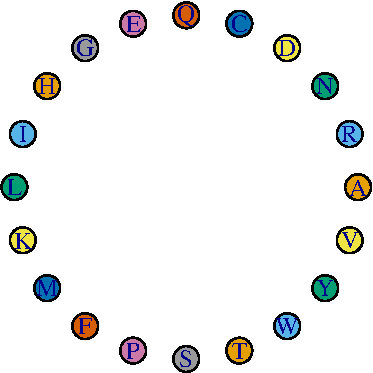
\includegraphics{lbrb_files/figure-latex/unnamed-chunk-448-1.pdf}

In theory, all mutations can change any codon into any other codon. We can represent mutations that result in a changed in the amino acid by connecting each amino acid with an arrow. We'll do this for adenine. Thicker arrows represent more common transitions.\\
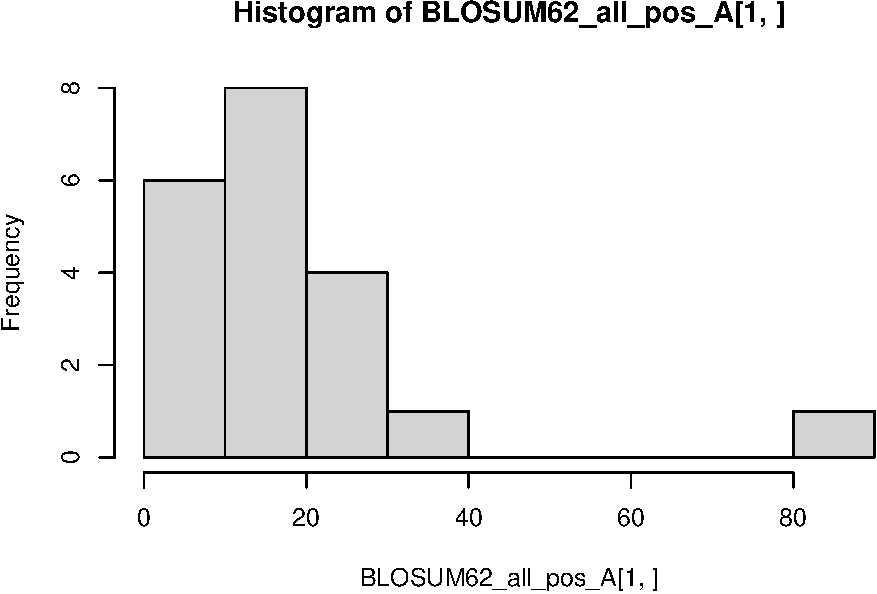
\includegraphics{lbrb_files/figure-latex/unnamed-chunk-449-1.pdf} 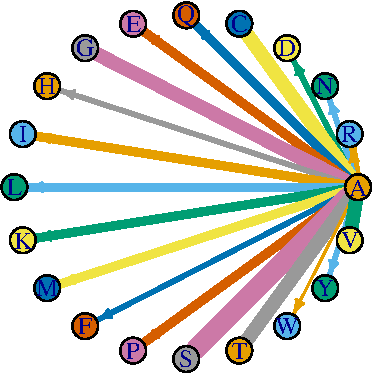
\includegraphics{lbrb_files/figure-latex/unnamed-chunk-449-2.pdf}

Often, there will be no change in a codon, the changes don't impact which amino acid, or a mutation to a different codon is reversed due to a \textbf{back mutation}. We can represent the fact that an adenine can stay as adenine with a \textbf{self loop}. You can see that the most common ``transition'' is for adenine to remain as adenine.

\begin{Shaded}
\begin{Highlighting}[]
\NormalTok{blosum.graph.A }\OtherTok{\textless{}{-}} \FunctionTok{graph\_from\_adjacency\_matrix}\NormalTok{(BLOSUM62\_all\_pos\_A,}
                                              \AttributeTok{diag =}\NormalTok{ T,}
                                              \AttributeTok{weighted =}\NormalTok{ T,}
                                              \AttributeTok{mode =} \StringTok{"directed"}\NormalTok{)}


\FunctionTok{plot.igraph}\NormalTok{(blosum.graph.A ,}
            \AttributeTok{layout =}\NormalTok{ blosum.graph.circle, }
            \AttributeTok{edge.arrow.size =}\FloatTok{0.5}\NormalTok{,}
            \AttributeTok{vertex.color=} \DecValTok{1}\SpecialCharTok{:}\DecValTok{20}\NormalTok{, }
            \AttributeTok{edge.color =} \DecValTok{1}\SpecialCharTok{:}\DecValTok{20}\NormalTok{,}
            \AttributeTok{edge.width =} \FunctionTok{E}\NormalTok{(blosum.graph.A)}\SpecialCharTok{$}\NormalTok{weight}\SpecialCharTok{/}\DecValTok{10}
\NormalTok{            )}
\end{Highlighting}
\end{Shaded}

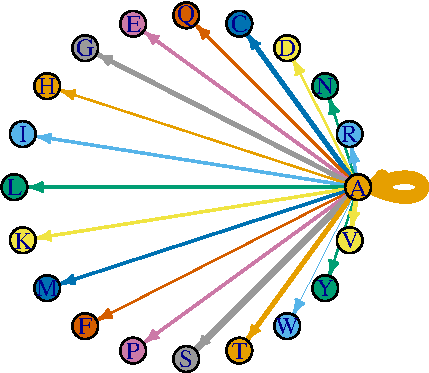
\includegraphics{lbrb_files/figure-latex/unnamed-chunk-450-1.pdf}

Instead of laying things out in circle, we can have them oriented so that the amino acids adenine is most likely to transition to are closest to it.

\begin{Shaded}
\begin{Highlighting}[]
\NormalTok{blosum.graph.A }\OtherTok{\textless{}{-}} \FunctionTok{graph\_from\_adjacency\_matrix}\NormalTok{(BLOSUM62\_all\_pos\_A,}
                                              \AttributeTok{diag =}\NormalTok{ F,}
                                              \AttributeTok{weighted =}\NormalTok{ T,}
                                              \AttributeTok{mode =} \StringTok{"directed"}\NormalTok{)}
\FunctionTok{plot.igraph}\NormalTok{(blosum.graph.A ,}
            \CommentTok{\#layout = blosum.graph.circle, }
            \AttributeTok{edge.arrow.size =}\FloatTok{0.5}\NormalTok{,}
            \AttributeTok{vertex.color=} \DecValTok{1}\SpecialCharTok{:}\DecValTok{20}\NormalTok{, }
            \AttributeTok{edge.color =} \DecValTok{1}\SpecialCharTok{:}\DecValTok{20}\NormalTok{,}
            \AttributeTok{edge.width =} \FunctionTok{E}\NormalTok{(blosum.graph.A)}\SpecialCharTok{$}\NormalTok{weight}\SpecialCharTok{/}\DecValTok{10}
\NormalTok{            )}
\end{Highlighting}
\end{Shaded}

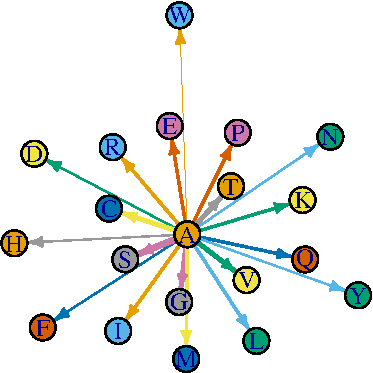
\includegraphics{lbrb_files/figure-latex/unnamed-chunk-451-1.pdf}

We can extend this by considering all possible transition and making a plot that tries to orient each amino acid close to the other amino acids its likely to transition to, and far from those its unlikely to. This is a bit tricky, since all transitions are now being consider.

\begin{Shaded}
\begin{Highlighting}[]
\NormalTok{blosum.graph.all }\OtherTok{\textless{}{-}} \FunctionTok{graph\_from\_adjacency\_matrix}\NormalTok{(BLOSUM62\_all\_pos,}
                                              \AttributeTok{diag =}\NormalTok{ F,}
                                              \AttributeTok{weighted =}\NormalTok{ T,}
                                              \AttributeTok{mode =} \StringTok{"directed"}\NormalTok{)}
\FunctionTok{plot.igraph}\NormalTok{(blosum.graph.all,}
            \AttributeTok{edge.arrow.size =} \DecValTok{0}\NormalTok{,}
            \AttributeTok{vertex.color=} \DecValTok{1}\SpecialCharTok{:}\DecValTok{20}\NormalTok{,}
            \AttributeTok{edge.color =} \DecValTok{1}\NormalTok{)}
\end{Highlighting}
\end{Shaded}

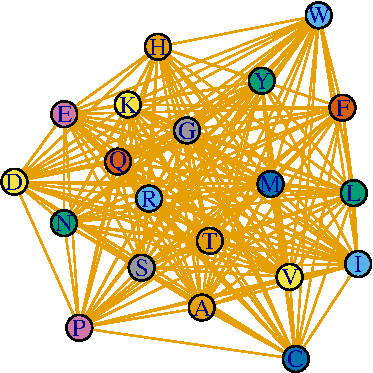
\includegraphics{lbrb_files/figure-latex/unnamed-chunk-452-1.pdf}

\hypertarget{a-complete-bioinformatics-workflow-in-r}{%
\chapter{A complete bioinformatics workflow in R}\label{a-complete-bioinformatics-workflow-in-r}}

\textbf{By}: Nathan L. Brouwer

\hypertarget{worked-example-building-a-phylogeny-in-r}{%
\chapter{``Worked example: Building a phylogeny in R''}\label{worked-example-building-a-phylogeny-in-r}}

\hypertarget{introduction-4}{%
\section{Introduction}\label{introduction-4}}

Phylogenies play an important role in computational biology and bioinformatics. Phylogenetics itself is an obligatly computational field that only began rapid growth when computational power allowed the many algorithms it relies on to be done rapidly. Phylogeneies of species, genes and proteins are used to address many biological issues, including

\begin{itemize}
\tightlist
\item
  Patterns of protein evolution
\item
  Origin and evolution of phenotypic traits
\item
  Origin and progression of epidemics
\item
  Origin of evolution of diseases (eg, zooenoses)
\item
  Prediction of protein function from its sequence
\item
  \ldots{} and many more
\end{itemize}

The actual building of a phylogeny is a computationally intensive task; moreover, there are many bioinformatics and computational tasks the precede the construction of a phylogeny:

\begin{itemize}
\tightlist
\item
  genome sequencing and assembly
\item
  computational gene prediction and annotation
\item
  database searching and results screening
\item
  pairwise sequence alignment
\item
  data organization and cleaning
\item
  multiple sequence alignment
\item
  evaluation and validation of alignment accuracy
\end{itemize}

Once all of these steps have been carried out, the building of a phylogeny involves

\begin{itemize}
\tightlist
\item
  picking a model of sequence evolution or other description of evolution
\item
  picking a statistical approach to tree construction
\item
  evaluationg uncertainty in the final tree
\end{itemize}

In this chapter we will work through many of these steps. In most cases we will pick the easiest or fastest option; in later chapters we will unpack the various options. This chapter is written as an interactive R sessions. You can follow along by opening the .Rmd file of the chapter or typing the appropriate commands into your own script. I assume that all the necessary packages have been installed and they only need to be loaded into R using the \emph{library()} command.

This lesson walks you through and entire workflow for a bioinformatics, including

\begin{enumerate}
\def\labelenumi{\arabic{enumi}.}
\tightlist
\item
  obtaining FASTA sequences
\item
  cleaning sequences
\item
  creating alignments
\item
  creating distance a distance matrix
\item
  building a phylogenetic tree
\end{enumerate}

We'll examine the Shroom family of genes, which produces Shroom proteins essential for tissue formation in many multicellular eukaryotes, including neural tube formation in vertebrates. We'll examine shroom in severall very different organism, including humans, mice and sea urchins. There is more than one type of shroom in vertebrates, and we'll also look at two different Shroom genes: shroom 1 and shroom 2.

This lesson draws on skills from previous sections of the book, but is written to act as a independent summary of these activities. There is therefore review of key aspects of R and bioinformatics throughout it.

\hypertarget{software-preliminaires}{%
\section{Software Preliminaires}\label{software-preliminaires}}

\hypertarget{vocab-4}{%
\subsection{Vocab}\label{vocab-4}}

\begin{itemize}
\tightlist
\item
  arguement
\item
  function
\item
  list
\item
  named list
\item
  vector
\item
  named vector
\item
  for() loop
\item
  R console
\end{itemize}

\hypertarget{r-functions-1}{%
\subsection{R functions}\label{r-functions-1}}

\begin{itemize}
\tightlist
\item
  library()
\item
  round()
\item
  plot()
\item
  mtext()
\item
  nchar()
\item
  rentrez::entrez\_fetch()
\item
  combio4all::entrez\_fetch\_list()
\item
  combio4aal::print\_msa() (Coghlan 2011)
\item
  Biostrings::AAStringSet()
\item
  msa::msa()
\item
  msa::msaConvert()
\item
  msa::msaPrettyPrint()
\item
  seqinr::dist.alignment()
\item
  ape::nj()
\end{itemize}

A few things need to be done to get started with our R session.

\hypertarget{download-necessary-packages}{%
\subsection{Download necessary packages}\label{download-necessary-packages}}

Many \emph{R} sessions begin by downloading necessary software packages to augment \emph{R's} functionality.

If you don't have them already, you'll need the following packages from CRAN:

\begin{enumerate}
\def\labelenumi{\arabic{enumi}.}
\tightlist
\item
  \texttt{ape}
\item
  \texttt{seqinr}
\item
  \texttt{rentrez}
\item
  \texttt{devtools}
\end{enumerate}

The CRAN packages can be loaded with \texttt{install.packages()}.

You'll also need these packages from Bioconductor:

\begin{enumerate}
\def\labelenumi{\arabic{enumi}.}
\tightlist
\item
  \texttt{msa}
\item
  \texttt{Biostrings}
\end{enumerate}

For install packages from Bioconductor, see the chapter at the beginning of this book on this process.

Finally, you'll need this package from GitHub

\begin{enumerate}
\def\labelenumi{\arabic{enumi}.}
\tightlist
\item
  \texttt{compbio4all}
\end{enumerate}

To install packages from GitHub you can use the code \texttt{devtools::install\_github("brouwern/combio4all")}

\hypertarget{load-packages-into-memory}{%
\subsection{Load packages into memory}\label{load-packages-into-memory}}

We noew need to load up all our bioinformatics and phylogenetics software into R. This is done with the \texttt{library()} command.

To run this code just clock on the sideways green triangel all the way to the right of the code.

NOTE: You'll likely see some red code appear on your screen. No worries, totally normal!

\begin{Shaded}
\begin{Highlighting}[]
\CommentTok{\# github packages}
\FunctionTok{library}\NormalTok{(compbio4all)}

\CommentTok{\# CRAN packages}
\FunctionTok{library}\NormalTok{(rentrez)}
\FunctionTok{library}\NormalTok{(seqinr)}
\FunctionTok{library}\NormalTok{(ape)}

\CommentTok{\# Bioconductor packages}
\FunctionTok{library}\NormalTok{(msa)}
\FunctionTok{library}\NormalTok{(Biostrings)}
\end{Highlighting}
\end{Shaded}

\hypertarget{downloading-macro-molecular-sequences}{%
\section{Downloading macro-molecular sequences}\label{downloading-macro-molecular-sequences}}

We're going to explore some sequences. First we need to download them. To do this we'll use a function, \texttt{entrez\_fretch()}, which accesses the \href{ncbi.nlm.nih.gov/search/}{\textbf{Entrez}} system of database (ncbi.nlm.nih.gov/search/). This function is from the \texttt{rentrez} package, which stands for ``R-Entrez.''

We need to tell \texttt{entrez\_fetch()} several things

\begin{enumerate}
\def\labelenumi{\arabic{enumi}.}
\tightlist
\item
  \texttt{db\ =\ ...} the type of entrez database.\\
\item
  \texttt{id\ =\ ...} the \textbf{accession} (ID) number of the sequence
\item
  \texttt{rettype\ =\ ...} file type what we want the function to return.
\end{enumerate}

Formally, these things are called \textbf{arguements} by \emph{R}.

We'll use these settings:

\begin{enumerate}
\def\labelenumi{\arabic{enumi}.}
\tightlist
\item
  \texttt{db\ =\ "protein"} to access the Entrez database of protein sequences\\
\item
  \texttt{rettype\ =\ "fasta"}, which is a standard file format for nucleic acid and protein sequences
\end{enumerate}

We'll set \texttt{id\ =\ ...} to sequences whose \textbf{accession numbers} are:

\begin{enumerate}
\def\labelenumi{\arabic{enumi}.}
\tightlist
\item
  NP\_065910: Human shroom 3
\item
  AAF13269: Mouse shroom 3a
\item
  CAA58534: Human shroom 2
\item
  XP\_783573: Sea urchin shroom
\end{enumerate}

There are two highly conserved regions of shroom 3
1. ASD 1: aa 884 to aa 1062 in hShroom3
1. ASD 2: aa 1671 to aa 1955 in hShroom3

Normally we'd have to download these sequences by hand through pointing and clicking on GeneBank records on the NCBI website. In \emph{R} we can do it automatically; this might take a second.

All the code needed is this:

\begin{Shaded}
\begin{Highlighting}[]
\CommentTok{\# Human shroom 3 (H. sapiens)}
\NormalTok{hShroom3 }\OtherTok{\textless{}{-}} \FunctionTok{entrez\_fetch}\NormalTok{(}\AttributeTok{db =} \StringTok{"protein"}\NormalTok{, }
                          \AttributeTok{id =} \StringTok{"NP\_065910"}\NormalTok{, }
                          \AttributeTok{rettype =} \StringTok{"fasta"}\NormalTok{)}
\end{Highlighting}
\end{Shaded}

The output is in FASTA format; we'll use the \texttt{cat()} to do a little formating for us:

\begin{Shaded}
\begin{Highlighting}[]
\FunctionTok{cat}\NormalTok{(hShroom3)}
\end{Highlighting}
\end{Shaded}

\begin{verbatim}
## >NP_065910.3 protein Shroom3 [Homo sapiens]
## MMRTTEDFHKPSATLNSNTATKGRYIYLEAFLEGGAPWGFTLKGGLEHGEPLIISKVEEGGKADTLSSKL
## QAGDEVVHINEVTLSSSRKEAVSLVKGSYKTLRLVVRRDVCTDPGHADTGASNFVSPEHLTSGPQHRKAA
## WSGGVKLRLKHRRSEPAGRPHSWHTTKSGEKQPDASMMQISQGMIGPPWHQSYHSSSSTSDLSNYDHAYL
## RRSPDQCSSQGSMESLEPSGAYPPCHLSPAKSTGSIDQLSHFHNKRDSAYSSFSTSSSILEYPHPGISGR
## ERSGSMDNTSARGGLLEGMRQADIRYVKTVYDTRRGVSAEYEVNSSALLLQGREARASANGQGYDKWSNI
## PRGKGVPPPSWSQQCPSSLETATDNLPPKVGAPLPPARSDSYAAFRHRERPSSWSSLDQKRLCRPQANSL
## GSLKSPFIEEQLHTVLEKSPENSPPVKPKHNYTQKAQPGQPLLPTSIYPVPSLEPHFAQVPQPSVSSNGM
## LYPALAKESGYIAPQGACNKMATIDENGNQNGSGRPGFAFCQPLEHDLLSPVEKKPEATAKYVPSKVHFC
## SVPENEEDASLKRHLTPPQGNSPHSNERKSTHSNKPSSHPHSLKCPQAQAWQAGEDKRSSRLSEPWEGDF
## QEDHNANLWRRLEREGLGQSLSGNFGKTKSAFSSLQNIPESLRRHSSLELGRGTQEGYPGGRPTCAVNTK
## AEDPGRKAAPDLGSHLDRQVSYPRPEGRTGASASFNSTDPSPEEPPAPSHPHTSSLGRRGPGPGSASALQ
## GFQYGKPHCSVLEKVSKFEQREQGSQRPSVGGSGFGHNYRPHRTVSTSSTSGNDFEETKAHIRFSESAEP
## LGNGEQHFKNGELKLEEASRQPCGQQLSGGASDSGRGPQRPDARLLRSQSTFQLSSEPEREPEWRDRPGS
## PESPLLDAPFSRAYRNSIKDAQSRVLGATSFRRRDLELGAPVASRSWRPRPSSAHVGLRSPEASASASPH
## TPRERHSVTPAEGDLARPVPPAARRGARRRLTPEQKKRSYSEPEKMNEVGIVEEAEPAPLGPQRNGMRFP
## ESSVADRRRLFERDGKACSTLSLSGPELKQFQQSALADYIQRKTGKRPTSAAGCSLQEPGPLRERAQSAY
## LQPGPAALEGSGLASASSLSSLREPSLQPRREATLLPATVAETQQAPRDRSSSFAGGRRLGERRRGDLLS
## GANGGTRGTQRGDETPREPSSWGARAGKSMSAEDLLERSDVLAGPVHVRSRSSPATADKRQDVLLGQDSG
## FGLVKDPCYLAGPGSRSLSCSERGQEEMLPLFHHLTPRWGGSGCKAIGDSSVPSECPGTLDHQRQASRTP
## CPRPPLAGTQGLVTDTRAAPLTPIGTPLPSAIPSGYCSQDGQTGRQPLPPYTPAMMHRSNGHTLTQPPGP
## RGCEGDGPEHGVEEGTRKRVSLPQWPPPSRAKWAHAAREDSLPEESSAPDFANLKHYQKQQSLPSLCSTS
## DPDTPLGAPSTPGRISLRISESVLRDSPPPHEDYEDEVFVRDPHPKATSSPTFEPLPPPPPPPPSQETPV
## YSMDDFPPPPPHTVCEAQLDSEDPEGPRPSFNKLSKVTIARERHMPGAAHVVGSQTLASRLQTSIKGSEA
## ESTPPSFMSVHAQLAGSLGGQPAPIQTQSLSHDPVSGTQGLEKKVSPDPQKSSEDIRTEALAKEIVHQDK
## SLADILDPDSRLKTTMDLMEGLFPRDVNLLKENSVKRKAIQRTVSSSGCEGKRNEDKEAVSMLVNCPAYY
## SVSAPKAELLNKIKEMPAEVNEEEEQADVNEKKAELIGSLTHKLETLQEAKGSLLTDIKLNNALGEEVEA
## LISELCKPNEFDKYRMFIGDLDKVVNLLLSLSGRLARVENVLSGLGEDASNEERSSLYEKRKILAGQHED
## ARELKENLDRRERVVLGILANYLSEEQLQDYQHFVKMKSTLLIEQRKLDDKIKLGQEQVKCLLESLPSDF
## IPKAGALALPPNLTSEPIPAGGCTFSGIFPTLTSPL
\end{verbatim}

Note the initial \texttt{\textgreater{}}, then the header line of \texttt{NP\_065910.3\ protein\ Shroom3\ {[}Homo\ sapiens{]}}. After that is the amino acid sequence. The underlying data also includes the \textbf{newline character} \texttt{\textbackslash{}n} to designate where each line of amino acids stops.

We can get the rest of the data by just chaing the \texttt{id\ =\ ...} argument:

\begin{Shaded}
\begin{Highlighting}[]
\CommentTok{\# Mouse shroom 3a (M. musculus)}
\NormalTok{mShroom3a }\OtherTok{\textless{}{-}} \FunctionTok{entrez\_fetch}\NormalTok{(}\AttributeTok{db =} \StringTok{"protein"}\NormalTok{, }
                          \AttributeTok{id =} \StringTok{"AAF13269"}\NormalTok{, }
                          \AttributeTok{rettype =} \StringTok{"fasta"}\NormalTok{)}

\CommentTok{\# Human shroom 2 (H. sapiens)}
\NormalTok{hShroom2 }\OtherTok{\textless{}{-}} \FunctionTok{entrez\_fetch}\NormalTok{(}\AttributeTok{db =} \StringTok{"protein"}\NormalTok{, }
                          \AttributeTok{id =} \StringTok{"CAA58534"}\NormalTok{, }
                          \AttributeTok{rettype =} \StringTok{"fasta"}\NormalTok{)}


\CommentTok{\# Sea{-}urchin shroom}
\NormalTok{sShroom }\OtherTok{\textless{}{-}} \FunctionTok{entrez\_fetch}\NormalTok{(}\AttributeTok{db =} \StringTok{"protein"}\NormalTok{, }
                          \AttributeTok{id =} \StringTok{"XP\_783573"}\NormalTok{, }
                          \AttributeTok{rettype =} \StringTok{"fasta"}\NormalTok{)}
\end{Highlighting}
\end{Shaded}

I'm going to check about how long each of these sequences is - each should have an at least slightly different length. If any are identical, I might have repeated an accession name or re-used an object name. The function \texttt{nchar()} counts of the number of characters in an \emph{R} object.

\begin{Shaded}
\begin{Highlighting}[]
\FunctionTok{nchar}\NormalTok{(hShroom3)}
\end{Highlighting}
\end{Shaded}

\begin{verbatim}
## [1] 2070
\end{verbatim}

\begin{Shaded}
\begin{Highlighting}[]
\FunctionTok{nchar}\NormalTok{(mShroom3a)}
\end{Highlighting}
\end{Shaded}

\begin{verbatim}
## [1] 2083
\end{verbatim}

\begin{Shaded}
\begin{Highlighting}[]
\FunctionTok{nchar}\NormalTok{(sShroom)}
\end{Highlighting}
\end{Shaded}

\begin{verbatim}
## [1] 1758
\end{verbatim}

\begin{Shaded}
\begin{Highlighting}[]
\FunctionTok{nchar}\NormalTok{(hShroom2)}
\end{Highlighting}
\end{Shaded}

\begin{verbatim}
## [1] 1673
\end{verbatim}

\hypertarget{prepping-macromolecular-sequences}{%
\section{Prepping macromolecular sequences}\label{prepping-macromolecular-sequences}}

\begin{quote}
``90\% of data analysis is data cleaning'' (-Just about every data analyst and data scientist on twitter)
\end{quote}

We have our sequences, but the current format isn't directly usable for us yet because there are several thigns that aren't sequence information

\begin{enumerate}
\def\labelenumi{\arabic{enumi}.}
\tightlist
\item
  metadata (the header)
\item
  page formatting information (the newline character)
\end{enumerate}

We can remove this non-sequence information using a function I wrote called \texttt{fasta\_cleaner()}, which is in the \texttt{compbio4all} package. The function uses \textbf{regular expressions} to remove the info we don't need.

\textbf{ASIDE}: If we run the name of the command with out any quotation marks we can see the code:

\begin{Shaded}
\begin{Highlighting}[]
\NormalTok{fasta\_cleaner}
\end{Highlighting}
\end{Shaded}

\begin{verbatim}
## function(fasta_object, parse = TRUE){
## 
##   fasta_object <- sub("^(>)(.*?)(\\n)(.*)(\\n\\n)","\\4",fasta_object)
##   fasta_object <- gsub("\n", "", fasta_object)
## 
##   if(parse == TRUE){
##     fasta_object <- stringr::str_split(fasta_object,
##                                        pattern = "",
##                                        simplify = FALSE)
##   }
## 
##   return(fasta_object[[1]])
## }
## <bytecode: 0x7fda36f05d60>
## <environment: namespace:compbio4all>
\end{verbatim}

\textbf{End ASIDE}

Now use the function to clean our sequences; we won't worry about what \texttt{pare\ =\ ...} is for.

\begin{Shaded}
\begin{Highlighting}[]
\NormalTok{hShroom3  }\OtherTok{\textless{}{-}} \FunctionTok{fasta\_cleaner}\NormalTok{(hShroom3,  }\AttributeTok{parse =}\NormalTok{ F)}
\NormalTok{mShroom3a }\OtherTok{\textless{}{-}} \FunctionTok{fasta\_cleaner}\NormalTok{(mShroom3a, }\AttributeTok{parse =}\NormalTok{ F)}
\NormalTok{hShroom2  }\OtherTok{\textless{}{-}} \FunctionTok{fasta\_cleaner}\NormalTok{(hShroom2,  }\AttributeTok{parse =}\NormalTok{ F)}
\NormalTok{sShroom   }\OtherTok{\textless{}{-}} \FunctionTok{fasta\_cleaner}\NormalTok{(sShroom,   }\AttributeTok{parse =}\NormalTok{ F)}
\end{Highlighting}
\end{Shaded}

Now let's take a peek at what our sequences look like:

\begin{Shaded}
\begin{Highlighting}[]
\NormalTok{hShroom3}
\end{Highlighting}
\end{Shaded}

\begin{verbatim}
## [1] "MMRTTEDFHKPSATLNSNTATKGRYIYLEAFLEGGAPWGFTLKGGLEHGEPLIISKVEEGGKADTLSSKLQAGDEVVHINEVTLSSSRKEAVSLVKGSYKTLRLVVRRDVCTDPGHADTGASNFVSPEHLTSGPQHRKAAWSGGVKLRLKHRRSEPAGRPHSWHTTKSGEKQPDASMMQISQGMIGPPWHQSYHSSSSTSDLSNYDHAYLRRSPDQCSSQGSMESLEPSGAYPPCHLSPAKSTGSIDQLSHFHNKRDSAYSSFSTSSSILEYPHPGISGRERSGSMDNTSARGGLLEGMRQADIRYVKTVYDTRRGVSAEYEVNSSALLLQGREARASANGQGYDKWSNIPRGKGVPPPSWSQQCPSSLETATDNLPPKVGAPLPPARSDSYAAFRHRERPSSWSSLDQKRLCRPQANSLGSLKSPFIEEQLHTVLEKSPENSPPVKPKHNYTQKAQPGQPLLPTSIYPVPSLEPHFAQVPQPSVSSNGMLYPALAKESGYIAPQGACNKMATIDENGNQNGSGRPGFAFCQPLEHDLLSPVEKKPEATAKYVPSKVHFCSVPENEEDASLKRHLTPPQGNSPHSNERKSTHSNKPSSHPHSLKCPQAQAWQAGEDKRSSRLSEPWEGDFQEDHNANLWRRLEREGLGQSLSGNFGKTKSAFSSLQNIPESLRRHSSLELGRGTQEGYPGGRPTCAVNTKAEDPGRKAAPDLGSHLDRQVSYPRPEGRTGASASFNSTDPSPEEPPAPSHPHTSSLGRRGPGPGSASALQGFQYGKPHCSVLEKVSKFEQREQGSQRPSVGGSGFGHNYRPHRTVSTSSTSGNDFEETKAHIRFSESAEPLGNGEQHFKNGELKLEEASRQPCGQQLSGGASDSGRGPQRPDARLLRSQSTFQLSSEPEREPEWRDRPGSPESPLLDAPFSRAYRNSIKDAQSRVLGATSFRRRDLELGAPVASRSWRPRPSSAHVGLRSPEASASASPHTPRERHSVTPAEGDLARPVPPAARRGARRRLTPEQKKRSYSEPEKMNEVGIVEEAEPAPLGPQRNGMRFPESSVADRRRLFERDGKACSTLSLSGPELKQFQQSALADYIQRKTGKRPTSAAGCSLQEPGPLRERAQSAYLQPGPAALEGSGLASASSLSSLREPSLQPRREATLLPATVAETQQAPRDRSSSFAGGRRLGERRRGDLLSGANGGTRGTQRGDETPREPSSWGARAGKSMSAEDLLERSDVLAGPVHVRSRSSPATADKRQDVLLGQDSGFGLVKDPCYLAGPGSRSLSCSERGQEEMLPLFHHLTPRWGGSGCKAIGDSSVPSECPGTLDHQRQASRTPCPRPPLAGTQGLVTDTRAAPLTPIGTPLPSAIPSGYCSQDGQTGRQPLPPYTPAMMHRSNGHTLTQPPGPRGCEGDGPEHGVEEGTRKRVSLPQWPPPSRAKWAHAAREDSLPEESSAPDFANLKHYQKQQSLPSLCSTSDPDTPLGAPSTPGRISLRISESVLRDSPPPHEDYEDEVFVRDPHPKATSSPTFEPLPPPPPPPPSQETPVYSMDDFPPPPPHTVCEAQLDSEDPEGPRPSFNKLSKVTIARERHMPGAAHVVGSQTLASRLQTSIKGSEAESTPPSFMSVHAQLAGSLGGQPAPIQTQSLSHDPVSGTQGLEKKVSPDPQKSSEDIRTEALAKEIVHQDKSLADILDPDSRLKTTMDLMEGLFPRDVNLLKENSVKRKAIQRTVSSSGCEGKRNEDKEAVSMLVNCPAYYSVSAPKAELLNKIKEMPAEVNEEEEQADVNEKKAELIGSLTHKLETLQEAKGSLLTDIKLNNALGEEVEALISELCKPNEFDKYRMFIGDLDKVVNLLLSLSGRLARVENVLSGLGEDASNEERSSLYEKRKILAGQHEDARELKENLDRRERVVLGILANYLSEEQLQDYQHFVKMKSTLLIEQRKLDDKIKLGQEQVKCLLESLPSDFIPKAGALALPPNLTSEPIPAGGCTFSGIFPTLTSPL"
\end{verbatim}

\hypertarget{aligning-sequences}{%
\section{Aligning sequences}\label{aligning-sequences}}

We can do a \href{https://tinyurl.com/y4du73zq}{\textbf{global alignment}} of one sequence against another using the \texttt{pairwiseAlignment()} function from the \textbf{Bioconductor} package \texttt{Biostrings} (note that capital ``B'' in \texttt{Biostrings}; most \emph{R} package names are all lower case, but not this one).

Let's align human versus mouse shroom:

\begin{Shaded}
\begin{Highlighting}[]
\NormalTok{align.h3.vs.m3a }\OtherTok{\textless{}{-}}\NormalTok{ Biostrings}\SpecialCharTok{::}\FunctionTok{pairwiseAlignment}\NormalTok{(}
\NormalTok{                  hShroom3,}
\NormalTok{                  mShroom3a)}
\end{Highlighting}
\end{Shaded}

We can peek at the alignment

\begin{Shaded}
\begin{Highlighting}[]
\NormalTok{align.h3.vs.m3a}
\end{Highlighting}
\end{Shaded}

\begin{verbatim}
## Global PairwiseAlignmentsSingleSubject (1 of 1)
## pattern: MMRTTEDFHKPSATLN-SNTATKGRYIYLEAFLE...KAGALALPPNLTSEPIPAGGCTFSGIFPTLTSPL
## subject: MK-TPENLEEPSATPNPSRTPTE-RFVYLEALLE...KAGAISLPPALTGHATPGGTSVFGGVFPTLTSPL
## score: 2189.934
\end{verbatim}

The \textbf{score} tells us how closely they are aligned; higher scores mean the sequences are more similar. Its hard to interpret the number on its own so we can get the \textbf{percent sequence identity (PID)} using the \texttt{pid()} function.

\begin{Shaded}
\begin{Highlighting}[]
\NormalTok{Biostrings}\SpecialCharTok{::}\FunctionTok{pid}\NormalTok{(align.h3.vs.m3a)}
\end{Highlighting}
\end{Shaded}

\begin{verbatim}
## [1] 70.56511
\end{verbatim}

So, \emph{shroom3} from humans and \emph{shroom3} from mice are \textasciitilde71\% similar (at least using this particular method of alignment, and there are many ways to do this!)

What about human shroom 3 and sea-urchin shroom?

\begin{Shaded}
\begin{Highlighting}[]
\NormalTok{align.h3.vs.h2 }\OtherTok{\textless{}{-}}\NormalTok{ Biostrings}\SpecialCharTok{::}\FunctionTok{pairwiseAlignment}\NormalTok{(}
\NormalTok{                  hShroom3,}
\NormalTok{                  hShroom2)}
\end{Highlighting}
\end{Shaded}

First check out the score using \texttt{score()}, which accesses it directly without all the other information.

\begin{Shaded}
\begin{Highlighting}[]
\FunctionTok{score}\NormalTok{(align.h3.vs.h2)}
\end{Highlighting}
\end{Shaded}

\begin{verbatim}
## [1] -5673.853
\end{verbatim}

Now the percent sequence alignment with \texttt{pid()}:

\begin{Shaded}
\begin{Highlighting}[]
\NormalTok{Biostrings}\SpecialCharTok{::}\FunctionTok{pid}\NormalTok{(align.h3.vs.h2)}
\end{Highlighting}
\end{Shaded}

\begin{verbatim}
## [1] 33.83277
\end{verbatim}

So Human shroom 3 and Mouse shroom 3 are 71\% identical, but Human shroom 3 and human shroom 2 are only 34\% similar? How does it work out evolutionary that a human and mouse gene are more similar than a human and a human gene? What are the evolutionary relationships among these genes within the shroom gene family?

\hypertarget{the-shroom-family-of-genes}{%
\section{The shroom family of genes}\label{the-shroom-family-of-genes}}

I've copied a table from a published paper which has accession numbers for 15 different Shroom genes.

\begin{Shaded}
\begin{Highlighting}[]
\NormalTok{shroom\_table }\OtherTok{\textless{}{-}} \FunctionTok{c}\NormalTok{(}\StringTok{"CAA78718"}\NormalTok{ , }\StringTok{"X. laevis Apx"}\NormalTok{ ,         }\StringTok{"xShroom1"}\NormalTok{,}
            \StringTok{"NP\_597713"}\NormalTok{ , }\StringTok{"H. sapiens APXL2"}\NormalTok{ ,     }\StringTok{"hShroom1"}\NormalTok{,}
            \StringTok{"CAA58534"}\NormalTok{ , }\StringTok{"H. sapiens APXL"}\NormalTok{,        }\StringTok{"hShroom2"}\NormalTok{,}
            \StringTok{"ABD19518"}\NormalTok{ , }\StringTok{"M. musculus Apxl"}\NormalTok{ ,      }\StringTok{"mShroom2"}\NormalTok{,}
            \StringTok{"AAF13269"}\NormalTok{ , }\StringTok{"M. musculus ShroomL"}\NormalTok{ ,   }\StringTok{"mShroom3a"}\NormalTok{,}
            \StringTok{"AAF13270"}\NormalTok{ , }\StringTok{"M. musculus ShroomS"}\NormalTok{ ,   }\StringTok{"mShroom3b"}\NormalTok{,}
            \StringTok{"NP\_065910"}\NormalTok{, }\StringTok{"H. sapiens Shroom"}\NormalTok{ ,     }\StringTok{"hShroom3"}\NormalTok{,}
            \StringTok{"ABD59319"}\NormalTok{ , }\StringTok{"X. laevis Shroom{-}like"}\NormalTok{,  }\StringTok{"xShroom3"}\NormalTok{,}
            \StringTok{"NP\_065768"}\NormalTok{, }\StringTok{"H. sapiens KIAA1202"}\NormalTok{ ,   }\StringTok{"hShroom4a"}\NormalTok{,}
            \StringTok{"AAK95579"}\NormalTok{ , }\StringTok{"H. sapiens SHAP{-}A"}\NormalTok{ ,     }\StringTok{"hShroom4b"}\NormalTok{,}
            \CommentTok{\#"DQ435686" , "M. musculus KIAA1202" ,  "mShroom4",}
            \StringTok{"ABA81834"}\NormalTok{ , }\StringTok{"D. melanogaster Shroom"}\NormalTok{, }\StringTok{"dmShroom"}\NormalTok{,}
            \StringTok{"EAA12598"}\NormalTok{ , }\StringTok{"A. gambiae Shroom"}\NormalTok{,      }\StringTok{"agShroom"}\NormalTok{,}
            \StringTok{"XP\_392427"}\NormalTok{ , }\StringTok{"A. mellifera Shroom"}\NormalTok{ ,  }\StringTok{"amShroom"}\NormalTok{,}
            \StringTok{"XP\_783573"}\NormalTok{ , }\StringTok{"S. purpuratus Shroom"}\NormalTok{ , }\StringTok{"spShroom"}\NormalTok{) }\CommentTok{\#sea urchin}
\end{Highlighting}
\end{Shaded}

I'll do a bit of formatting; you can ignore these details if you want

\begin{Shaded}
\begin{Highlighting}[]
\CommentTok{\# convert to matrix}
\NormalTok{shroom\_table\_matrix }\OtherTok{\textless{}{-}} \FunctionTok{matrix}\NormalTok{(shroom\_table,}
                                  \AttributeTok{byrow =}\NormalTok{ T,}
                                  \AttributeTok{nrow =} \DecValTok{14}\NormalTok{)}
\CommentTok{\# convert to dataframe}
\NormalTok{shroom\_table }\OtherTok{\textless{}{-}} \FunctionTok{data.frame}\NormalTok{(shroom\_table\_matrix, }
                     \AttributeTok{stringsAsFactors =}\NormalTok{ F)}

\CommentTok{\# name columns}
\FunctionTok{names}\NormalTok{(shroom\_table) }\OtherTok{\textless{}{-}} \FunctionTok{c}\NormalTok{(}\StringTok{"accession"}\NormalTok{, }\StringTok{"name.orig"}\NormalTok{,}\StringTok{"name.new"}\NormalTok{)}

\CommentTok{\# Create simplified species names}
\NormalTok{shroom\_table}\SpecialCharTok{$}\NormalTok{spp }\OtherTok{\textless{}{-}} \StringTok{"Homo"}
\NormalTok{shroom\_table}\SpecialCharTok{$}\NormalTok{spp[}\FunctionTok{grep}\NormalTok{(}\StringTok{"laevis"}\NormalTok{,shroom\_table}\SpecialCharTok{$}\NormalTok{name.orig)] }\OtherTok{\textless{}{-}} \StringTok{"Xenopus"}
\NormalTok{shroom\_table}\SpecialCharTok{$}\NormalTok{spp[}\FunctionTok{grep}\NormalTok{(}\StringTok{"musculus"}\NormalTok{,shroom\_table}\SpecialCharTok{$}\NormalTok{name.orig)] }\OtherTok{\textless{}{-}} \StringTok{"Mus"}
\NormalTok{shroom\_table}\SpecialCharTok{$}\NormalTok{spp[}\FunctionTok{grep}\NormalTok{(}\StringTok{"melanogaster"}\NormalTok{,shroom\_table}\SpecialCharTok{$}\NormalTok{name.orig)] }\OtherTok{\textless{}{-}} \StringTok{"Drosophila"}
\NormalTok{shroom\_table}\SpecialCharTok{$}\NormalTok{spp[}\FunctionTok{grep}\NormalTok{(}\StringTok{"gambiae"}\NormalTok{,shroom\_table}\SpecialCharTok{$}\NormalTok{name.orig)] }\OtherTok{\textless{}{-}} \StringTok{"mosquito"}
\NormalTok{shroom\_table}\SpecialCharTok{$}\NormalTok{spp[}\FunctionTok{grep}\NormalTok{(}\StringTok{"mellifera"}\NormalTok{,shroom\_table}\SpecialCharTok{$}\NormalTok{name.orig)] }\OtherTok{\textless{}{-}} \StringTok{"bee"}
\NormalTok{shroom\_table}\SpecialCharTok{$}\NormalTok{spp[}\FunctionTok{grep}\NormalTok{(}\StringTok{"purpuratus"}\NormalTok{,shroom\_table}\SpecialCharTok{$}\NormalTok{name.orig)] }\OtherTok{\textless{}{-}} \StringTok{"sea urchin"}
\end{Highlighting}
\end{Shaded}

Take a look:

\begin{Shaded}
\begin{Highlighting}[]
\NormalTok{shroom\_table}
\end{Highlighting}
\end{Shaded}

\begin{verbatim}
##    accession              name.orig  name.new        spp
## 1   CAA78718          X. laevis Apx  xShroom1    Xenopus
## 2  NP_597713       H. sapiens APXL2  hShroom1       Homo
## 3   CAA58534        H. sapiens APXL  hShroom2       Homo
## 4   ABD19518       M. musculus Apxl  mShroom2        Mus
## 5   AAF13269    M. musculus ShroomL mShroom3a        Mus
## 6   AAF13270    M. musculus ShroomS mShroom3b        Mus
## 7  NP_065910      H. sapiens Shroom  hShroom3       Homo
## 8   ABD59319  X. laevis Shroom-like  xShroom3    Xenopus
## 9  NP_065768    H. sapiens KIAA1202 hShroom4a       Homo
## 10  AAK95579      H. sapiens SHAP-A hShroom4b       Homo
## 11  ABA81834 D. melanogaster Shroom  dmShroom Drosophila
## 12  EAA12598      A. gambiae Shroom  agShroom   mosquito
## 13 XP_392427    A. mellifera Shroom  amShroom        bee
## 14 XP_783573   S. purpuratus Shroom  spShroom sea urchin
\end{verbatim}

\hypertarget{downloading-multiple-sequences}{%
\section{Downloading multiple sequences}\label{downloading-multiple-sequences}}

Instead of getting one sequence at a time we can download several by accessing the ``accession'' column from the table

\begin{Shaded}
\begin{Highlighting}[]
\NormalTok{shroom\_table}\SpecialCharTok{$}\NormalTok{accession}
\end{Highlighting}
\end{Shaded}

\begin{verbatim}
##  [1] "CAA78718"  "NP_597713" "CAA58534"  "ABD19518"  "AAF13269"  "AAF13270" 
##  [7] "NP_065910" "ABD59319"  "NP_065768" "AAK95579"  "ABA81834"  "EAA12598" 
## [13] "XP_392427" "XP_783573"
\end{verbatim}

We can give this whole set of accessions to \texttt{entrez\_fetch()}:

\begin{Shaded}
\begin{Highlighting}[]
\NormalTok{shrooms }\OtherTok{\textless{}{-}} \FunctionTok{entrez\_fetch}\NormalTok{(}\AttributeTok{db =} \StringTok{"protein"}\NormalTok{, }
                          \AttributeTok{id =}\NormalTok{ shroom\_table}\SpecialCharTok{$}\NormalTok{accession, }
                          \AttributeTok{rettype =} \StringTok{"fasta"}\NormalTok{)}
\end{Highlighting}
\end{Shaded}

We can look at what we got here with \texttt{cat()} (I won't display this because it is very long!)

\begin{Shaded}
\begin{Highlighting}[]
\FunctionTok{cat}\NormalTok{(shrooms)}
\end{Highlighting}
\end{Shaded}

The current format of these data is a single, long set of data. This is a standard way to store, share and transmit FASTA files, but in \emph{R} we'll need a slightly different format.

We'll download all of the sequences again, this time using a function from \texttt{compbio4all} called \texttt{entrez\_fetch\_list()} which is a \textbf{wrapper} function I wrote to put the output of \texttt{entrez\_fetch()} into an \emph{R} data format called a \textbf{list}.

\begin{Shaded}
\begin{Highlighting}[]
\NormalTok{shrooms\_list }\OtherTok{\textless{}{-}} \FunctionTok{entrez\_fetch\_list}\NormalTok{(}\AttributeTok{db =} \StringTok{"protein"}\NormalTok{, }
                          \AttributeTok{id =}\NormalTok{ shroom\_table}\SpecialCharTok{$}\NormalTok{accession, }
                          \AttributeTok{rettype =} \StringTok{"fasta"}\NormalTok{)}
\end{Highlighting}
\end{Shaded}

Now we have a list which as 14 \textbf{elements}, one for each sequence in our table.

\begin{Shaded}
\begin{Highlighting}[]
\FunctionTok{length}\NormalTok{(shrooms\_list)}
\end{Highlighting}
\end{Shaded}

\begin{verbatim}
## [1] 14
\end{verbatim}

We now need to clean up each one fo these sequences. We can do that using a simple \texttt{for()} loop:

\begin{Shaded}
\begin{Highlighting}[]
\ControlFlowTok{for}\NormalTok{(i }\ControlFlowTok{in} \DecValTok{1}\SpecialCharTok{:}\FunctionTok{length}\NormalTok{(shrooms\_list))\{}
\NormalTok{  shrooms\_list[[i]] }\OtherTok{\textless{}{-}} \FunctionTok{fasta\_cleaner}\NormalTok{(shrooms\_list[[i]], }\AttributeTok{parse =}\NormalTok{ F)}
\NormalTok{\}}
\end{Highlighting}
\end{Shaded}

Second to last step: we need to take each one of our sequences from our list and put it into a \textbf{vector}, in particular a \textbf{named vector}

\begin{Shaded}
\begin{Highlighting}[]
\CommentTok{\# make a vector to store output}
\NormalTok{shrooms\_vector }\OtherTok{\textless{}{-}} \FunctionTok{rep}\NormalTok{(}\ConstantTok{NA}\NormalTok{, }\FunctionTok{length}\NormalTok{(shrooms\_list))}

\CommentTok{\# run the loop}
\ControlFlowTok{for}\NormalTok{(i }\ControlFlowTok{in} \DecValTok{1}\SpecialCharTok{:}\FunctionTok{length}\NormalTok{(shrooms\_vector))\{}
\NormalTok{  shrooms\_vector[i] }\OtherTok{\textless{}{-}}\NormalTok{ shrooms\_list[[i]]}
\NormalTok{\}}

\CommentTok{\# name the vector}
\FunctionTok{names}\NormalTok{(shrooms\_vector) }\OtherTok{\textless{}{-}} \FunctionTok{names}\NormalTok{(shrooms\_list)}
\end{Highlighting}
\end{Shaded}

Now the final step: we need to convert our named vector to a \textbf{string set} using \texttt{Biostrings::AAStringSet()}. Note the \texttt{\_ss} tag at the end of the object we're assigning the output to, which designates this as a string set.

\begin{Shaded}
\begin{Highlighting}[]
\NormalTok{shrooms\_vector\_ss }\OtherTok{\textless{}{-}}\NormalTok{ Biostrings}\SpecialCharTok{::}\FunctionTok{AAStringSet}\NormalTok{(shrooms\_vector)}
\end{Highlighting}
\end{Shaded}

\hypertarget{multiple-sequence-alignment}{%
\section{Multiple sequence alignment}\label{multiple-sequence-alignment}}

We must \textbf{align} all of the sequences we downloaded and use that \textbf{alignment} to build a \textbf{phylogenetic tree}. This will tell us how the different genes, both within and between species, are likely to be related.

\hypertarget{building-an-multiple-sequence-alignment-msa}{%
\subsection{Building an Multiple Sequence Alignment (MSA)}\label{building-an-multiple-sequence-alignment-msa}}

We'll use the software \texttt{msa,} which implements the \textbf{ClustalW} multiple sequence alignment algorithm. Normally we'd have to download the ClustalW program and either point-and-click our way through it or use the \textbf{command line}*, but these folks wrote up the algorithm in R so we can do this with a line of R code. This will take a second or two.

\begin{Shaded}
\begin{Highlighting}[]
\NormalTok{shrooms\_align }\OtherTok{\textless{}{-}} \FunctionTok{msa}\NormalTok{(shrooms\_vector\_ss,}
                     \AttributeTok{method =} \StringTok{"ClustalW"}\NormalTok{)}
\end{Highlighting}
\end{Shaded}

\begin{verbatim}
## use default substitution matrix
\end{verbatim}

\hypertarget{viewing-an-msa}{%
\subsection{Viewing an MSA}\label{viewing-an-msa}}

Once we build an MSA we need to visualize it.

\hypertarget{viewing-an-msa-in-r}{%
\subsubsection{Viewing an MSA in R}\label{viewing-an-msa-in-r}}

We can look at the output from \texttt{msa()}, but its not very helpful

\begin{Shaded}
\begin{Highlighting}[]
\NormalTok{shrooms\_align}
\end{Highlighting}
\end{Shaded}

\begin{verbatim}
## CLUSTAL 2.1  
## 
## Call:
##    msa(shrooms_vector_ss, method = "ClustalW")
## 
## MsaAAMultipleAlignment with 14 rows and 2252 columns
##      aln                                                   names
##  [1] -------------------------...------------------------- NP_065768
##  [2] -------------------------...------------------------- AAK95579
##  [3] -------------------------...SVFGGVFPTLTSPL----------- AAF13269
##  [4] -------------------------...SVFGGVFPTLTSPL----------- AAF13270
##  [5] -------------------------...CTFSGIFPTLTSPL----------- NP_065910
##  [6] -------------------------...NKS--LPPPLTSSL----------- ABD59319
##  [7] -------------------------...------------------------- CAA58534
##  [8] -------------------------...------------------------- ABD19518
##  [9] -------------------------...LT----------------------- NP_597713
## [10] -------------------------...------------------------- CAA78718
## [11] -------------------------...------------------------- EAA12598
## [12] -------------------------...------------------------- ABA81834
## [13] MTELQPSPPGYRVQDEAPGPPSCPP...------------------------- XP_392427
## [14] -------------------------...AATSSSSNGIGGPEQLNSNATSSYC XP_783573
##  Con -------------------------...------------------------- Consensus
\end{verbatim}

A function called \texttt{print\_msa()} (Coghlan 2011) which I've put into\texttt{combio4all} can give us more informative output by printing out the actual alignment into the R console.

To use \texttt{print\_msa()} We need to make a few minor tweaks though first. These are behind the scenes changes so don't worry about the details right now. We'll change the name to \texttt{shrooms\_align\_seqinr} to indcate that one of our changes is putting this into a format defined by the bioinformatics package \texttt{seqinr}.

\begin{Shaded}
\begin{Highlighting}[]
\FunctionTok{class}\NormalTok{(shrooms\_align) }\OtherTok{\textless{}{-}} \StringTok{"AAMultipleAlignment"}
\NormalTok{shrooms\_align\_seqinr }\OtherTok{\textless{}{-}} \FunctionTok{msaConvert}\NormalTok{(shrooms\_align, }\AttributeTok{type =} \StringTok{"seqinr::alignment"}\NormalTok{)}
\end{Highlighting}
\end{Shaded}

I won't display the output from \texttt{shrooms\_align\_seqinr} because its very long; we have 14 shroom genes, and shroom happens to be a rather long gene.

\begin{Shaded}
\begin{Highlighting}[]
\FunctionTok{print\_msa}\NormalTok{(}\AttributeTok{alignment =}\NormalTok{ shrooms\_align\_seqinr, }
          \AttributeTok{chunksize =} \DecValTok{60}\NormalTok{)}
\end{Highlighting}
\end{Shaded}

\hypertarget{displaying-an-msa-as-an-r-plot}{%
\subsubsection{Displaying an MSA as an R plot}\label{displaying-an-msa-as-an-r-plot}}

I'm going to just show about 100 amino acids near the end of the alignment, where there is the most overlap across all of the sequences. This is set with the \texttt{start\ =\ ...} and \texttt{end\ =\ ...} arguments. Note that we're using the \texttt{shrooms\_align} object.

\begin{Shaded}
\begin{Highlighting}[]
\NormalTok{ggmsa}\SpecialCharTok{::}\FunctionTok{ggmsa}\NormalTok{(shrooms\_align,   }\CommentTok{\# shrooms\_align, NOT shrooms\_align\_seqinr}
      \AttributeTok{start =} \DecValTok{2000}\NormalTok{, }
      \AttributeTok{end =} \DecValTok{2100}\NormalTok{) }
\end{Highlighting}
\end{Shaded}

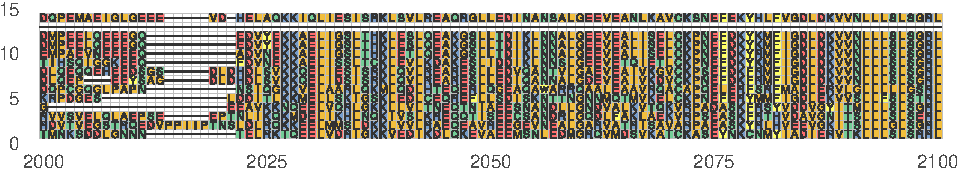
\includegraphics{lbrb_files/figure-latex/unnamed-chunk-482-1.pdf}

\hypertarget{saving-an-msa-as-pdf}{%
\subsubsection{Saving an MSA as PDF}\label{saving-an-msa-as-pdf}}

We can take a look at the alignment in PDF format if we want. I this case I'm going to just show about 100 amino acids near the end of the alignment, where there is the most overlap across all of the sequences. This is set with the \texttt{y\ =\ c(...)} argument.

\begin{Shaded}
\begin{Highlighting}[]
\FunctionTok{msaPrettyPrint}\NormalTok{(shrooms\_align,             }\CommentTok{\# alignment}
               \AttributeTok{file =} \StringTok{"shroom\_msa.pdf"}\NormalTok{,   }\CommentTok{\# file name}
               \AttributeTok{y=}\FunctionTok{c}\NormalTok{(}\DecValTok{2000}\NormalTok{, }\DecValTok{2100}\NormalTok{),           }\CommentTok{\# range}
               \AttributeTok{askForOverwrite=}\ConstantTok{FALSE}\NormalTok{)}
\end{Highlighting}
\end{Shaded}

You can see where R is saving thigns by running \texttt{getwd()}

\begin{Shaded}
\begin{Highlighting}[]
\FunctionTok{getwd}\NormalTok{()}
\end{Highlighting}
\end{Shaded}

\begin{verbatim}
## [1] "/Users/nlb24/google_backup_sync_nlb24/lbrb"
\end{verbatim}

On a Mac you can usually find the file by searching in Finder for the file name, which I set to be ``shroom\_msa.pdf'' using the \texttt{file\ =\ ...} arguement above.

\hypertarget{genetic-distance.}{%
\section{Genetic distance.}\label{genetic-distance.}}

Next need to first get an estimate of how similar each sequences is. The more amino acids that are identical to each other, the more similar.

Instead of similarity, we usually work in terms of \emph{difference} or \textbf{genetic distance} (a.k.a. \textbf{evolutionary distance}). This is done with the \texttt{dist.alignment()} function.

\begin{Shaded}
\begin{Highlighting}[]
\NormalTok{shrooms\_dist }\OtherTok{\textless{}{-}}\NormalTok{ seqinr}\SpecialCharTok{::}\FunctionTok{dist.alignment}\NormalTok{(shrooms\_align\_seqinr, }
                                       \AttributeTok{matrix =} \StringTok{"identity"}\NormalTok{)}
\end{Highlighting}
\end{Shaded}

We've made a matrix using \texttt{dist.alignment()}; let's round it off so its easier to look at using the \texttt{round()} function.

\begin{Shaded}
\begin{Highlighting}[]
\NormalTok{shrooms\_dist\_rounded }\OtherTok{\textless{}{-}} \FunctionTok{round}\NormalTok{(shrooms\_dist,}
                              \AttributeTok{digits =} \DecValTok{3}\NormalTok{)}
\end{Highlighting}
\end{Shaded}

Now let's look at it

\begin{Shaded}
\begin{Highlighting}[]
\NormalTok{shrooms\_dist\_rounded}
\end{Highlighting}
\end{Shaded}

\begin{verbatim}
##           NP_065768 AAK95579 AAF13269 AAF13270 NP_065910 ABD59319 CAA58534
## AAK95579      0.000                                                       
## AAF13269      0.884    0.917                                              
## AAF13270      0.897    0.917    0.000                                     
## NP_065910     0.878    0.912    0.533    0.536                            
## ABD59319      0.893    0.921    0.783    0.783     0.782                  
## CAA58534      0.872    0.908    0.838    0.849     0.840    0.864         
## ABD19518      0.866    0.912    0.834    0.846     0.838    0.855    0.548
## NP_597713     0.916    0.939    0.903    0.903     0.902    0.904    0.896
## CAA78718      0.925    0.955    0.896    0.895     0.893    0.893    0.898
## EAA12598      0.914    0.947    0.899    0.899     0.902    0.897    0.891
## ABA81834      0.938    0.943    0.935    0.934     0.936    0.940    0.935
## XP_392427     0.936    0.963    0.935    0.934     0.938    0.941    0.938
## XP_783573     0.940    0.958    0.942    0.939     0.942    0.935    0.942
##           ABD19518 NP_597713 CAA78718 EAA12598 ABA81834 XP_392427
## AAK95579                                                         
## AAF13269                                                         
## AAF13270                                                         
## NP_065910                                                        
## ABD59319                                                         
## CAA58534                                                         
## ABD19518                                                         
## NP_597713    0.900                                               
## CAA78718     0.891     0.919                                     
## EAA12598     0.896     0.920    0.922                            
## ABA81834     0.935     0.932    0.946    0.882                   
## XP_392427    0.934     0.927    0.947    0.878    0.923          
## XP_783573    0.946     0.947    0.941    0.925    0.954     0.943
\end{verbatim}

\hypertarget{phylognetic-trees-finally}{%
\section{Phylognetic trees (finally!)}\label{phylognetic-trees-finally}}

We got our sequence, built multiple sequence alignment, and calcualted the genetic distance between sequences. Now we are - finally - ready to build a phylogenetic tree.

First, we let R figure out the structure of the tree. There are \textbf{MANY} ways to build phylogenetic trees. We'll use a common one used for exploring sequences called \textbf{neighbor joining} algorithm via the function \texttt{nj()}. Neighbor joining uses genetic distances to cluster sequences into \textbf{clades}.

\begin{Shaded}
\begin{Highlighting}[]
\NormalTok{tree }\OtherTok{\textless{}{-}} \FunctionTok{nj}\NormalTok{(shrooms\_dist)}
\end{Highlighting}
\end{Shaded}

\hypertarget{plotting-phylogenetic-trees}{%
\subsection{Plotting phylogenetic trees}\label{plotting-phylogenetic-trees}}

Now we'll make a quick plot of our tree using \texttt{plot()} (and add a little label using a function called \texttt{mtext()}).

\begin{Shaded}
\begin{Highlighting}[]
\CommentTok{\# plot tree}
\FunctionTok{plot.phylo}\NormalTok{ (tree, }\AttributeTok{main=}\StringTok{"Phylogenetic Tree"}\NormalTok{, }
            \AttributeTok{type =} \StringTok{"unrooted"}\NormalTok{, }
            \AttributeTok{use.edge.length =}\NormalTok{ F)}

\CommentTok{\# add label}
\FunctionTok{mtext}\NormalTok{(}\AttributeTok{text =} \StringTok{"Shroom family gene tree {-} unrooted, no branch lengths"}\NormalTok{)}
\end{Highlighting}
\end{Shaded}

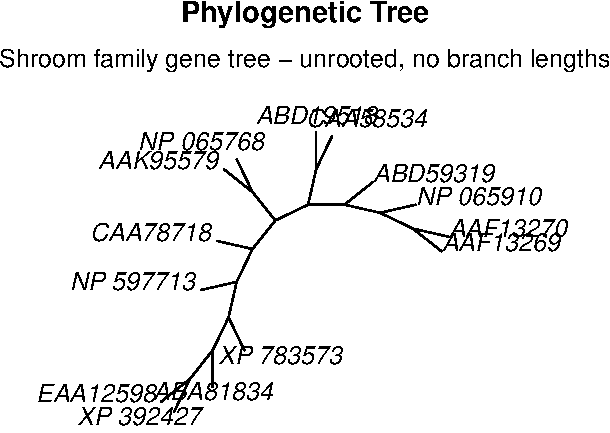
\includegraphics{lbrb_files/figure-latex/unnamed-chunk-489-1.pdf}

This is an **unrooted tree*. For the sake of plotting we've also ignored the evolutionary distance between the sequences.

To make a rooted tree we remove \texttt{type\ =\ "unrooted}.

\begin{Shaded}
\begin{Highlighting}[]
\CommentTok{\# plot tree}
\FunctionTok{plot.phylo}\NormalTok{ (tree, }\AttributeTok{main=}\StringTok{"Phylogenetic Tree"}\NormalTok{, }
            \AttributeTok{use.edge.length =}\NormalTok{ F)}

\CommentTok{\# add label}
\FunctionTok{mtext}\NormalTok{(}\AttributeTok{text =} \StringTok{"Shroom family gene tree {-} rooted, no branch lenths"}\NormalTok{)}
\end{Highlighting}
\end{Shaded}

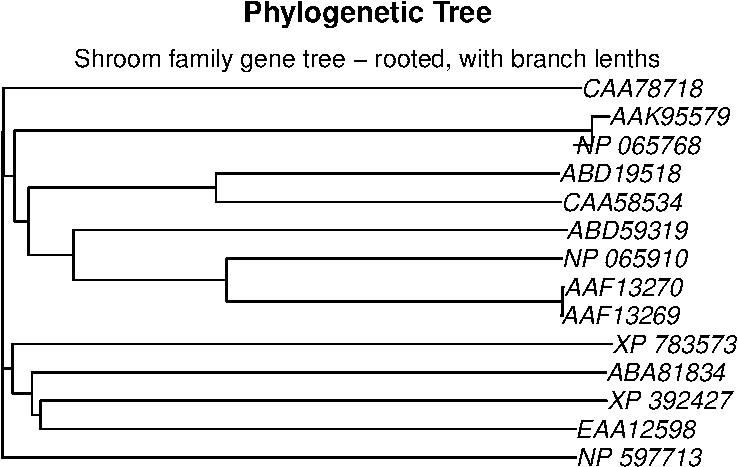
\includegraphics{lbrb_files/figure-latex/unnamed-chunk-490-1.pdf}

We can include information about branch length by setting \texttt{use.edge.length\ =\ ...} to \texttt{T}.

\begin{Shaded}
\begin{Highlighting}[]
\CommentTok{\# plot tree}
\FunctionTok{plot.phylo}\NormalTok{ (tree, }\AttributeTok{main=}\StringTok{"Phylogenetic Tree"}\NormalTok{, }
            \AttributeTok{use.edge.length =}\NormalTok{ T)}

\CommentTok{\# add label}
\FunctionTok{mtext}\NormalTok{(}\AttributeTok{text =} \StringTok{"Shroom family gene tree {-} rooted, with branch lenths"}\NormalTok{)}
\end{Highlighting}
\end{Shaded}

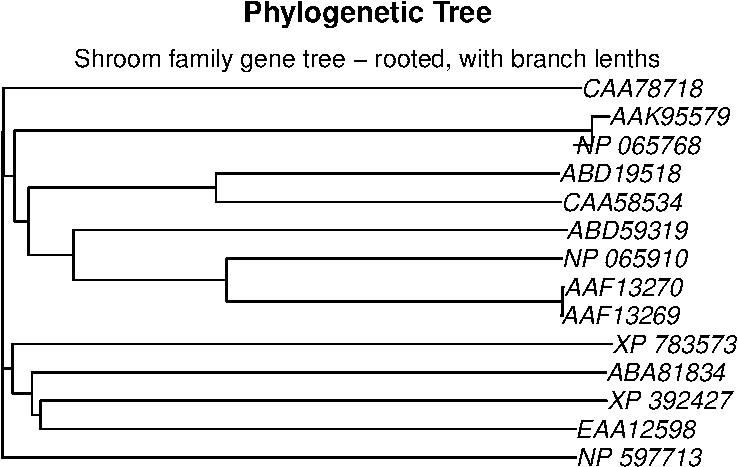
\includegraphics{lbrb_files/figure-latex/unnamed-chunk-491-1.pdf}

Some of the branches are now very short, but most are very long, indicating that these genes have been evolvin independently for many millions of years.

Let's make a fancier plot. Don't worry about all the steps; I've added some more code to add some annotations on the right-hand side to help us see what's going on.

\begin{Shaded}
\begin{Highlighting}[]
\FunctionTok{plot}\NormalTok{(tree, }\AttributeTok{main=}\StringTok{"Phylogenetic Tree"}\NormalTok{)}
\FunctionTok{mtext}\NormalTok{(}\AttributeTok{text =} \StringTok{"Shroom family gene tree"}\NormalTok{)}

\NormalTok{x }\OtherTok{\textless{}{-}} \FloatTok{0.551}
\NormalTok{x2 }\OtherTok{\textless{}{-}} \FloatTok{0.6}

\CommentTok{\# label Shrm 3}
\FunctionTok{segments}\NormalTok{(}\AttributeTok{x0 =}\NormalTok{ x, }\AttributeTok{y0 =} \DecValTok{1}\NormalTok{, }
         \AttributeTok{x1 =}\NormalTok{ x, }\AttributeTok{y1 =} \DecValTok{4}\NormalTok{,}
         \AttributeTok{lwd=}\DecValTok{2}\NormalTok{)}
\FunctionTok{text}\NormalTok{(}\AttributeTok{x =}\NormalTok{ x}\SpecialCharTok{*}\FloatTok{1.01}\NormalTok{, }\AttributeTok{y =} \FloatTok{2.5}\NormalTok{, }\StringTok{"Shrm 3"}\NormalTok{,}\AttributeTok{adj =} \DecValTok{0}\NormalTok{)}

\FunctionTok{segments}\NormalTok{(}\AttributeTok{x0 =}\NormalTok{ x, }\AttributeTok{y0 =} \DecValTok{5}\NormalTok{, }
         \AttributeTok{x1 =}\NormalTok{ x, }\AttributeTok{y1 =} \DecValTok{6}\NormalTok{,}
         \AttributeTok{lwd=}\DecValTok{2}\NormalTok{)}
\FunctionTok{text}\NormalTok{(}\AttributeTok{x =}\NormalTok{ x}\SpecialCharTok{*}\FloatTok{1.01}\NormalTok{, }\AttributeTok{y =} \FloatTok{5.5}\NormalTok{, }\StringTok{"Shrm 2"}\NormalTok{,}\AttributeTok{adj =} \DecValTok{0}\NormalTok{)}

\FunctionTok{segments}\NormalTok{(}\AttributeTok{x0 =}\NormalTok{ x, }\AttributeTok{y0 =} \DecValTok{7}\NormalTok{, }
         \AttributeTok{x1 =}\NormalTok{ x, }\AttributeTok{y1 =} \DecValTok{9}\NormalTok{,}
         \AttributeTok{lwd=}\DecValTok{2}\NormalTok{)}
\FunctionTok{text}\NormalTok{(}\AttributeTok{x =}\NormalTok{ x}\SpecialCharTok{*}\FloatTok{1.01}\NormalTok{, }\AttributeTok{y =} \DecValTok{8}\NormalTok{, }\StringTok{"Shrm 1"}\NormalTok{,}\AttributeTok{adj =} \DecValTok{0}\NormalTok{)}

\FunctionTok{segments}\NormalTok{(}\AttributeTok{x0 =}\NormalTok{ x, }\AttributeTok{y0 =} \DecValTok{10}\NormalTok{, }
         \AttributeTok{x1 =}\NormalTok{ x, }\AttributeTok{y1 =} \DecValTok{13}\NormalTok{,}
         \AttributeTok{lwd=}\DecValTok{2}\NormalTok{)}
\FunctionTok{text}\NormalTok{(}\AttributeTok{x =}\NormalTok{ x}\SpecialCharTok{*}\FloatTok{1.01}\NormalTok{, }\AttributeTok{y =} \DecValTok{12}\NormalTok{, }\StringTok{"Shrm ?"}\NormalTok{,}\AttributeTok{adj =} \DecValTok{0}\NormalTok{)}


\FunctionTok{segments}\NormalTok{(}\AttributeTok{x0 =}\NormalTok{ x, }\AttributeTok{y0 =} \DecValTok{14}\NormalTok{, }
         \AttributeTok{x1 =}\NormalTok{ x, }\AttributeTok{y1 =} \DecValTok{15}\NormalTok{,}
         \AttributeTok{lwd=}\DecValTok{2}\NormalTok{)}
\FunctionTok{text}\NormalTok{(}\AttributeTok{x =}\NormalTok{ x}\SpecialCharTok{*}\FloatTok{1.01}\NormalTok{, }\AttributeTok{y =} \FloatTok{14.5}\NormalTok{, }\StringTok{"Shrm 4"}\NormalTok{,}\AttributeTok{adj =} \DecValTok{0}\NormalTok{)}


\FunctionTok{segments}\NormalTok{(}\AttributeTok{x0 =}\NormalTok{ x2, }\AttributeTok{y0 =} \DecValTok{1}\NormalTok{, }
         \AttributeTok{x1 =}\NormalTok{ x2, }\AttributeTok{y1 =} \DecValTok{6}\NormalTok{,}
         \AttributeTok{lwd=}\DecValTok{2}\NormalTok{)}

\FunctionTok{segments}\NormalTok{(}\AttributeTok{x0 =}\NormalTok{ x2, }\AttributeTok{y0 =} \DecValTok{7}\NormalTok{, }
         \AttributeTok{x1 =}\NormalTok{ x2, }\AttributeTok{y1 =} \DecValTok{9}\NormalTok{,}
         \AttributeTok{lwd=}\DecValTok{2}\NormalTok{)}

\FunctionTok{segments}\NormalTok{(}\AttributeTok{x0 =}\NormalTok{ x2, }\AttributeTok{y0 =} \DecValTok{10}\NormalTok{, }
         \AttributeTok{x1 =}\NormalTok{ x2, }\AttributeTok{y1 =} \DecValTok{15}\NormalTok{,}
         \AttributeTok{lwd=}\DecValTok{2}\NormalTok{)}
\end{Highlighting}
\end{Shaded}

\includegraphics{lbrb_files/figure-latex/unnamed-chunk-492-1.pdf}

\hypertarget{calculating-genetic-distances-between-sequences}{%
\chapter{Calculating genetic distances between sequences}\label{calculating-genetic-distances-between-sequences}}

\textbf{By}: Nathan Brouwer, with some content adapted Coghlan (2011) \href{https://a-little-book-of-r-for-bioinformatics.readthedocs.io/en/latest/src/chapter5.html}{Multiple Alignment and Phylogenetic trees} and under the Creative Commons 3.0 Attribution License \href{https://creativecommons.org/licenses/by/3.0/}{(CC BY 3.0)}. Functions print\_msa() and clean\_alignment() adapted from (\href{https://a-little-book-of-r-for-bioinformatics.readthedocs.io/en/latest/\#}{Coglan 2011}).

\hypertarget{preliminaries-13}{%
\section{Preliminaries}\label{preliminaries-13}}

\begin{Shaded}
\begin{Highlighting}[]
\FunctionTok{library}\NormalTok{(compbio4all)}
\FunctionTok{library}\NormalTok{(msa)}
\FunctionTok{library}\NormalTok{(seqinr)}
\FunctionTok{library}\NormalTok{(ape)}
\end{Highlighting}
\end{Shaded}

\hypertarget{introduction-5}{%
\section{Introduction}\label{introduction-5}}

A common first step in performing a \textbf{phylogenetic analysis} is to calculate the \textbf{pairwise genetic distances} between sequences. The \textbf{genetic distance} is an estimate of the evolutionary \textbf{divergence} between two sequences, and is usually measured in quantity of evolutionary change, e.g., an estimate of the number of mutations that have occurred since the two sequences shared a \textbf{common ancestor}.

We can calculate the genetic distances between protein sequences using the \texttt{dist.alignment()} function in the \texttt{seqinr} package. The \texttt{dist.alignment()} function takes a multiple sequence alignment (MSA) as input. Based on the MSA that you give it, \texttt{dist.alignment()} calculates the genetic distance between each \textbf{\emph{pair}} of proteins in the multiple alignment, yielding pairwise distances. For example, to calculate genetic distances between the virus phosphoproteins based on the multiple sequence alignment stored in virusaln, we type:

\begin{Shaded}
\begin{Highlighting}[]
\FunctionTok{data}\NormalTok{(virusaln)}
\NormalTok{virusdist }\OtherTok{\textless{}{-}}\NormalTok{ seqinr}\SpecialCharTok{::}\FunctionTok{dist.alignment}\NormalTok{(virusaln\_seqinr)  }\CommentTok{\# Calculate the genetic distances}

\NormalTok{virusdist }\CommentTok{\# Print out the genetic distance matrix}
\end{Highlighting}
\end{Shaded}

\begin{verbatim}
##        P06747 P0C569 Q5VKP1
## P0C569      0              
## Q5VKP1      0      0       
## O56773      0      0      0
\end{verbatim}

\textbf{NOTE} My result are different from the original results, shown here:
I need to check the settings used for the MSA\\
P0C569 O56773 P06747
O56773 0.4142670
P06747 0.4678196 0.4714045
Q5VKP1 0.4828127 0.5067117 0.5034130

The genetic distance matrix above shows the genetic distance between each pair of proteins. The sequences are referred to by their \textbf{UniProt accessions}. Recall that

\begin{itemize}
\tightlist
\item
  P06747 = rabies virus phosphoprotein
\item
  P0C569 is Mokola virus phosphoprotein
\item
  O56773 is Lagos bat virus phosphoprotein
\item
  Q5VKP1 is Western Caucasian bat virus phosphoprotein.
\end{itemize}

Based on the genetic \textbf{distance matrix} above, we can see that the genetic distance between Lagos bat virus phosphoprotein (O56773) and Mokola virus phosphoprotein (P0C569) is smallest (about 0.414). Similarly, the genetic distance between Western Caucasian bat virus phosphoprotein (Q5VKP1) and Lagos bat virus phosphoprotein (O56773) is the biggest (about 0.507).

The larger the genetic distance between two sequences, the more amino acid changes (such as change from Asp to Met) or \textbf{indels} that have occurred since they shared a common ancestor, and the longer ago their \textbf{common ancestor} probably lived. (The relationship between number of mutations and time, however, depends on the mutation rate and generation time of the organism).

\hypertarget{calculating-genetic-distances-between-dnamrna-sequences}{%
\section{Calculating genetic distances between DNA/mRNA sequences}\label{calculating-genetic-distances-between-dnamrna-sequences}}

Just like for protein sequences, you can calculate genetic distances between DNA (or mRNA) sequences based on an alignment of the sequences. The RefSeq DNA accession numbers for the proteins we've been using are:

\begin{itemize}
\tightlist
\item
  AF049118 = mRNA sequence for Mokola virus phosphoprotein,
\item
  AF049114 = mRNA sequence for Mokola virus phosphoprotein,
\item
  AF049119 = mRNA sequence for Lagos bat virus phosphoprotein,
\item
  AF049115 = mRNA sequence for Duvenhage virus phosphoprotein.
\end{itemize}

We can retrieve these DNA sequences using \texttt{entrez\_fetch\_list()}. Some notes about how we'll use this function works:

\begin{enumerate}
\def\labelenumi{\arabic{enumi}.}
\tightlist
\item
  \texttt{db} is short for ``database''
\item
  the database is called \texttt{nuccore} (not \texttt{genebank} or \texttt{gene})
\item
  the argument \texttt{rettype} is ``tt''; I think it stands for ``REtURN type'' (I also forget the second ``t'')
\end{enumerate}

\begin{Shaded}
\begin{Highlighting}[]
\CommentTok{\# put accessions in vector}
\NormalTok{accessions\_mrna }\OtherTok{\textless{}{-}} \FunctionTok{c}\NormalTok{(}\StringTok{"AF049118"}\NormalTok{,}\StringTok{"AF049114"}\NormalTok{,}\StringTok{"AF049119"}\NormalTok{,}\StringTok{"AF049115"}\NormalTok{)}

\CommentTok{\# get sequences}
\NormalTok{virus\_mrna\_list }\OtherTok{\textless{}{-}} \FunctionTok{entrez\_fetch\_list}\NormalTok{(}\AttributeTok{db =} \StringTok{"nuccore"}\NormalTok{,  }\CommentTok{\# "nuccore" db for DNA }
                                   \AttributeTok{id =}\NormalTok{ accessions\_mrna, }
                                   \AttributeTok{rettype =} \StringTok{"FASTA"}\NormalTok{) }\CommentTok{\# rettype has two t}
\end{Highlighting}
\end{Shaded}

We can clean these three sequences using a simple \texttt{for()} loop. We set \texttt{parse\ =\ F} so we get things back as single character string.

\begin{Shaded}
\begin{Highlighting}[]
\ControlFlowTok{for}\NormalTok{(i }\ControlFlowTok{in} \DecValTok{1}\SpecialCharTok{:}\FunctionTok{length}\NormalTok{(virus\_mrna\_list))\{}
\NormalTok{  virus\_mrna\_list[[i]] }\OtherTok{\textless{}{-}} \FunctionTok{fasta\_cleaner}\NormalTok{(virus\_mrna\_list[i], }
                                       \AttributeTok{parse =}\NormalTok{ F)}
\NormalTok{\}}
\end{Highlighting}
\end{Shaded}

Now we need to convert each of these into a named vector of sequences.

\begin{Shaded}
\begin{Highlighting}[]
\NormalTok{mra\_seq\_vector }\OtherTok{\textless{}{-}} \FunctionTok{c}\NormalTok{(}\AttributeTok{AF049118 =}\NormalTok{  virus\_mrna\_list[[}\DecValTok{1}\NormalTok{]] ,}
                 \AttributeTok{AF049114 =}\NormalTok{ virus\_mrna\_list[[}\DecValTok{2}\NormalTok{]] ,}
                 \AttributeTok{AF049119 =}\NormalTok{ virus\_mrna\_list[[}\DecValTok{3}\NormalTok{]] ,}
                 \AttributeTok{AF049115 =}\NormalTok{ virus\_mrna\_list[[}\DecValTok{4}\NormalTok{]])}
\end{Highlighting}
\end{Shaded}

Finally convert this to a ``stringset'' using \texttt{Biostrings::DNAStringSet()}.

\begin{Shaded}
\begin{Highlighting}[]
\NormalTok{dna\_seq\_stringset }\OtherTok{\textless{}{-}}\NormalTok{ Biostrings}\SpecialCharTok{::}\FunctionTok{DNAStringSet}\NormalTok{(mra\_seq\_vector)}
\end{Highlighting}
\end{Shaded}

Let's see what we got

\begin{Shaded}
\begin{Highlighting}[]
\NormalTok{dna\_seq\_stringset}
\end{Highlighting}
\end{Shaded}

\begin{verbatim}
## DNAStringSet object of length 4:
##     width seq                                               names               
## [1]  1083 TCAGAGAGCTCCTTTGCAAAGGA...AAAATGAAAAAAACATTTAACAT AF049118
## [2]  1016 CACTTCGAACGGTACATATTAGT...AAATTCTCAAAAATGAGCTCTCC AF049114
## [3]  1010 CAAAATGTCATCTCATATGAAAT...GGAACTTAAAACACAGAAGGTTT AF049119
## [4]   990 ATGAGCAAGATTTTTATCAATCC...ACACCACTGACAAAATGAACATC AF049115
\end{verbatim}

Now we can make an alignment use \texttt{msa()}.

\begin{Shaded}
\begin{Highlighting}[]
\NormalTok{virus\_mrna\_aln }\OtherTok{\textless{}{-}} \FunctionTok{msa}\NormalTok{(}\AttributeTok{inputSeqs =}\NormalTok{ dna\_seq\_stringset,}
                     \AttributeTok{method =} \StringTok{"ClustalW"}\NormalTok{)}
\end{Highlighting}
\end{Shaded}

\begin{verbatim}
## use default substitution matrix
\end{verbatim}

The output looks like this

\begin{Shaded}
\begin{Highlighting}[]
\NormalTok{virus\_mrna\_aln}
\end{Highlighting}
\end{Shaded}

\begin{verbatim}
## CLUSTAL 2.1  
## 
## Call:
##    msa(inputSeqs = dna_seq_stringset, method = "ClustalW")
## 
## MsaDNAMultipleAlignment with 4 rows and 1097 columns
##     aln                                                    names
## [1] -------------------------C...------------------------- AF049114
## [2] --------------------------...------------------------- AF049119
## [3] TCAGAGAGCTCCTTTGCAAAGGAGGA...AAAAACATTTAACAT---------- AF049118
## [4] --------------------------...CAACACCACTGACAAAATGAACATC AF049115
## Con --------------------------...-??-??---?-???----------- Consensus
\end{verbatim}

This looks a LOT different than an amino acid alignment, which looked like this:

\begin{Shaded}
\begin{Highlighting}[]
\FunctionTok{data}\NormalTok{(virusaln)}
\NormalTok{virusaln}
\end{Highlighting}
\end{Shaded}

\begin{verbatim}
## AAMultipleAlignment with 4 rows and 306 columns
##      aln                                                    names               
## [1] MSKDLVHPSLIRAGIVELEMAEETTD...NDKVARLIQEDINSYMARLEEAE-- P0C569
## [2] MSKGLIHPSAIRSGLVDLEMAEETVD...TDKVARLMQDDIHNYMTRIEEIDHN O56773
## [3] MSKIFVNPSAIRAGLADLEMAEETVD...SNKLSKIMQDDLNRYTSC------- P06747
## [4] MSKSLIHPSDLRAGLADIEMADETVD...QDKLCKLMQEDLNAYSVSSNN---- Q5VKP1
\end{verbatim}

Why might the be different? First, examine the output above and determine how long the DNA alignment is versus the amino acid alignment? Why are they different, and why is one longer than the other?

The DNA alignment is 1097 columns, while the amino acid alignment is only 306 rows. Note that 306*3 = 918. 1097 is pretty close to 1097. What's the relevance of multiplying by 3?

\hypertarget{calculationg-genetic-distance}{%
\section{Calculationg genetic distance}\label{calculationg-genetic-distance}}

You can calculate a genetic distance for DNA or mRNA sequences using the \texttt{dist.dna()} function in the \texttt{ape} package. \texttt{dist.dna()} takes a MSA of DNA or mRNA sequences as its input, and calculates the genetic distance between each pair of DNA sequences in the multiple alignment.

The \texttt{dist.dna()} function requires the input alignment to be in a special format known as \texttt{DNAbin} format, so we must use the \texttt{as.DNAbin()} function to convert our DNA alignment into this format before using the \texttt{dist.dna()} function.

\begin{Shaded}
\begin{Highlighting}[]
 \CommentTok{\# Convert the alignment to "DNAbin" format}
\NormalTok{virus\_mrna\_aln\_bin }\OtherTok{\textless{}{-}}\NormalTok{ ape}\SpecialCharTok{::}\FunctionTok{as.DNAbin}\NormalTok{(virus\_mrna\_aln)}
\end{Highlighting}
\end{Shaded}

The output of \texttt{as.DNAbin()} gives us a short summery of the alignment

\begin{Shaded}
\begin{Highlighting}[]
\NormalTok{virus\_mrna\_aln\_bin}
\end{Highlighting}
\end{Shaded}

\begin{verbatim}
## 4 DNA sequences in binary format stored in a matrix.
## 
## All sequences of same length: 1097 
## 
## Labels:
## AF049114
## AF049119
## AF049118
## AF049115
## 
## Base composition:
##     a     c     g     t 
## 0.324 0.202 0.240 0.234 
## (Total: 4.39 kb)
\end{verbatim}

Now to make and view the alignment:

\begin{Shaded}
\begin{Highlighting}[]
 \CommentTok{\# Calculate the genetic distance matrix}
\NormalTok{virus\_mrna\_dist }\OtherTok{\textless{}{-}}\NormalTok{ ape}\SpecialCharTok{::}\FunctionTok{dist.dna}\NormalTok{(virus\_mrna\_aln\_bin)}

 \CommentTok{\# Print out the genetic distance matrix}
\NormalTok{virus\_mrna\_dist                             }
\end{Highlighting}
\end{Shaded}

\begin{verbatim}
##           AF049114  AF049119  AF049118
## AF049119 0.3400576                    
## AF049118 0.5235850 0.5637372          
## AF049115 0.6854129 0.6852311 0.7656023
\end{verbatim}

NOTE: my results for this alignment are the same as the original by Coghlan. I'm not sure why my amino acid alignment produces divergent results but the DNA is the same.

\hypertarget{unrooted-neighbor-joining-phylogenetic-trees}{%
\chapter{Unrooted neighbor-joining phylogenetic trees}\label{unrooted-neighbor-joining-phylogenetic-trees}}

\textbf{NOTE}: the code for this chapter works as intended but there are some differences between my results and what is reported by the original author of the chapter. This is likely to do with different alignment software, though it could just be a typo.

\textbf{By}: Avril Coghlan.
Multiple Alignment and Phylogenetic trees
\url{https://a-little-book-of-r-for-bioinformatics.readthedocs.io/en/latest/src/chapter5.html}

\textbf{Adapted, edited and expanded}: Nathan Brouwer under the Creative Commons 3.0 Attribution License \href{https://creativecommons.org/licenses/by/3.0/}{(CC BY 3.0)}.

\hypertarget{preliminaries-14}{%
\section{Preliminaries}\label{preliminaries-14}}

\begin{Shaded}
\begin{Highlighting}[]
\FunctionTok{library}\NormalTok{(compbio4all)}
\FunctionTok{library}\NormalTok{(seqinr)}
\end{Highlighting}
\end{Shaded}

You will need to install the \texttt{ape} package if you do not have it already using \texttt{install.packages("ape")}.

\begin{Shaded}
\begin{Highlighting}[]
\FunctionTok{library}\NormalTok{(ape)}
\end{Highlighting}
\end{Shaded}

\hypertarget{key-functions}{%
\subsection{Key functions}\label{key-functions}}

\begin{itemize}
\tightlist
\item
  compbio4all::unrooted\_NJ\_tree (Coghlan 200x)
\end{itemize}

\hypertarget{key-vocab}{%
\subsection{Key vocab}\label{key-vocab}}

\begin{itemize}
\tightlist
\item
  clade
\item
  bootstrap
\item
  resample
\item
  rooted vs.~unrooted tree
\item
  outgroup
\end{itemize}

\hypertarget{building-an-unrooted-phylogenetic-tree-for-protein-sequences}{%
\section{Building an unrooted phylogenetic tree for protein sequences}\label{building-an-unrooted-phylogenetic-tree-for-protein-sequences}}

Once we have a \textbf{distance matrix} that gives the \textbf{pairwise distances} between all our protein sequences, we can build a \textbf{phylogenetic tree} based on that distance matrix. One method for using this is the \textbf{neighbor-joining algorithm}.

If we have the distance matrix already made we can make the tree like this using \texttt{ape::nj()}. The distance matrix is saved in \texttt{compbio4all} as \texttt{virus\_mrna\_dist}. Load this with \texttt{data()}.

\begin{Shaded}
\begin{Highlighting}[]
\FunctionTok{par}\NormalTok{(}\AttributeTok{mfrow =} \FunctionTok{c}\NormalTok{(}\DecValTok{1}\NormalTok{,}\DecValTok{1}\NormalTok{))}
\CommentTok{\# load the distance matrix}
\FunctionTok{data}\NormalTok{(virus\_mrna\_dist)}

\CommentTok{\# build the tree}
\NormalTok{tree\_from\_distmat }\OtherTok{\textless{}{-}} \FunctionTok{nj}\NormalTok{(virus\_mrna\_dist)}


\FunctionTok{plot.phylo}\NormalTok{(tree\_from\_distmat, }\AttributeTok{type =} \StringTok{"unrooted"}\NormalTok{)}
\end{Highlighting}
\end{Shaded}

\includegraphics{lbrb_files/figure-latex/unnamed-chunk-508-1.pdf}

\hypertarget{build-tree-with-unrooted_nj_tree}{%
\subsection{\texorpdfstring{Build tree with \texttt{unrooted\_NJ\_tree()}}{Build tree with unrooted\_NJ\_tree()}}\label{build-tree-with-unrooted_nj_tree}}

Coghlan (2011) wrote a function to simply the steps of making an NJ tree. The R function \texttt{unrooted\_NJ\_tree()} is a \textbf{wrapper} for functions from the \texttt{ape} package which builds a phylogenetic tree based on an alignment of sequences, using the NJ algorithm.

The \texttt{unrooted\_NJ\_tree()} function takes an alignment of sequences its input, calculates \textbf{pairwise distances} between the sequences based on the alignment behind the scenes, and then builds a phylogenetic tree based on the pairwise distances. It returns the phylogenetic tree, and also makes a plot of that tree. It also gives us information about to what extent the data in the original MSA support the evolutionary relationships shown in the tree.

The alignment is saved in \texttt{compbio4all} as \texttt{virusaln} and can be loaded with the \texttt{data()} command.

\begin{Shaded}
\begin{Highlighting}[]
\FunctionTok{data}\NormalTok{(virusaln\_seqinr\_clean)}
\end{Highlighting}
\end{Shaded}

Take a look at the structure of the data

\begin{Shaded}
\begin{Highlighting}[]
\FunctionTok{str}\NormalTok{(virusaln\_seqinr\_clean)}
\end{Highlighting}
\end{Shaded}

\begin{verbatim}
## List of 4
##  $ nb : int 4
##  $ nam: chr [1:4] "P0C569" "O56773" "P06747" "Q5VKP1"
##  $ seq: chr [1:4] "MSKLVHPSIRAGIVELEMAEETTDLIRTIQAHLQGEPVDLPEDMRLIDREEEDEGDPFQFLDEGVKGEFRWSSIGYVNIMSTSIQTHSDESGEDEEVAHQVAESFSKKYKF"| __truncated__ "MSKLIHPSIRSGLVDLEMAEETVDLVKNLQAHLQGEPVDLPEDMKMLNSEEEEQGDPFQFLDEGVKGDFKWSSIGYVTFMPTSKQTSDSETDEDEEVAHQVAESFSKKYKF"| __truncated__ "MSKFVNPSIRAGLADLEMAEETVDLIRNIQAHLQGEPVDLPEDMRLLDSAERDEGDPFQYLDNGVRGEFKWSVISYVNFPPSDKQTSSSSTDD-EEIAHQIAESFSKKYKF"| __truncated__ "MSKLIHPSLRAGLADIEMADETVDLVKNLQAHLQGEPIKLPEGVKLIDREEEEEVDPFQFLDEGIKGEIKWSSISYVNFPPTDIQAHSS--DDAEEIAHQVAESYSKKYKF"| __truncated__
##  $ com: logi NA
##  - attr(*, "class")= chr "alignment"
\end{verbatim}

\begin{Shaded}
\begin{Highlighting}[]
\NormalTok{virusalntree }\OtherTok{\textless{}{-}} \FunctionTok{unrooted\_NJ\_tree}\NormalTok{(virusaln\_seqinr\_clean,}
                               \AttributeTok{type=}\StringTok{"protein"}\NormalTok{)}
\end{Highlighting}
\end{Shaded}

Note that you need to specify that the type of sequences that you are using are protein sequences when you use \texttt{unrooted\_NJ\_tree()}, by setting \texttt{type=protein}.

We can see that \texttt{Q5VKP1} (Western Caucasian bat virus phosphoprotein) and \texttt{P06747} (rabies virus phosphoprotein) have been grouped together into a \textbf{clade} on the tree, and that \texttt{O56773} (Lagos bat virus phosphoprotein) and \texttt{P0C569} (Mokola virus phosphoprotein) are grouped together.

This is consistent with what we saw above in the genetic distance matrix, which showed that the genetic distance between Lagos bat virus phosphoprotein (O56773) and Mokola virus phosphoprotein (P0C569) is relatively small.

\hypertarget{boostrap-values-indicate-support-for-clades}{%
\section{Boostrap values indicate support for clades}\label{boostrap-values-indicate-support-for-clades}}

In the plot, the numbers in blue boxes are \textbf{bootstrap values} for the nodes in the tree. A bootstrap value for a particular node in the tree gives an idea of the confidence that we have in the clade (group) defined by that node in the tree. If a node has a high bootstrap value (near 100\%) then we are very confident that the clade defined by the node is correct, while if it has a low bootstrap value (near 0\%) then we are not so confident.

Note that the fact that a bootstrap value for a node is high does not necessarily guarantee that the clade defined by the node is correct, but just tells us that it is quite likely that it is correct given the data and analysis we're using.

The bootstrap values are calculated by making many (for example, 100) random \textbf{resamples} of the alignment that the phylogenetic tree was based upon. Each resample of the alignment consists of a certain number x (e.g.. 200) of randomly sampled \emph{columns} from the alignment. Each resample of the alignment (e.g.. 200 randomly sampled columns) forms a sort of fake alignment of its own, and a phylogenetic tree can be based upon the \emph{resample}. We can make 100 random resamples of the alignment, and build 100 phylogenetic trees based on the 100 resamples. These 100 trees are known as the \textbf{bootstrap trees}. For each clade (grouping) that we see in our original phylogenetic tree, we can count in how many of the 100 bootstrap trees it appears. This is known as the \textbf{bootstrap value} for the clade in our original phylogenetic tree.

For example, if we calculate 100 random resamples of the virus phosphoprotein alignment, and build 100 phylogenetic trees based on these resamples, we can calculate the bootstrap values for each clade in the virus phosphoprotein phylogenetic tree.

\textbf{NOTE:} I am currently not able to reproduce these results:

In this case, the bootstrap value for the node defining the clade containing Q5VKP1 (Western Caucasian bat virus phosphoprotein) and P06747 (rabies virus phosphoprotein) is 25\%, while the bootstrap value for node defining the clade containing of Lagos bat virus phosphoprotein (O56773) and Mokola virus phosphoprotein (P0C569) is 100\%. The bootstrap values for each of these clades is the percent of 100 bootstrap trees that the clade appears in.

Therefore, we are very confident that Lagos bat virus and Mokola virus phosphoproteins should be grouped together in the tree. However, we are not so confident that the Western Caucasian bat virus and rabies virus phosphoproteins should be grouped together.

\hypertarget{branch-lengths-indicate-divergence-between-sequences}{%
\section{Branch lengths indicate divergence between sequences}\label{branch-lengths-indicate-divergence-between-sequences}}

The lengths of the branches in the plot of the tree are proportional to the amount of evolutionary change (estimated number of mutations) along the branches. In this case, the branches leading to Lagos bat virus phosphoprotein (O56773) and Mokola virus phosphoprotein (P0C569) from the node representing their common ancestor are slightly shorter than the branches leading to the Western Caucasian bat virus (Q5VKP1) and rabies virus (P06747) phosphoproteins from the node representing their common ancestor.

This suggests that there might have been more mutations in the Western Caucasian bat virus (Q5VKP1) and rabies virus (P06747) phosphoproteins since they shared a common ancestor, than in the Lagos bat virus phosphoprotein (O56773) and Mokola virus phosphoprotein (P0C569) since they shared a common ancestor.

\hypertarget{unrooted-trees-lack-an-outgroup}{%
\section{Unrooted trees lack an outgroup}\label{unrooted-trees-lack-an-outgroup}}

The tree above of the virus phosphoproteins is an \textbf{unrooted} phylogenetic tree as it does not contain an \textbf{outgroup} sequence; that is, a sequence of a protein that is known to be more distantly related to the other proteins in the tree than they are to each other.

As a result, we cannot tell which direction evolutionary time ran in along the internal branches of the tree. For example, we cannot tell whether the node representing the common ancestor of (O56773, P0C569) was an ancestor of the node representing the common ancestor of (Q5VKP1, P06747), or the other way around.

In order to build a \textbf{rooted }phylogenetic tree, we need to have an outgroup sequence in our tree. In the case of the virus phosphoproteins, this is unfortunately not possible, as there is not any protein known that is more distantly related to the four proteins already in our tree than they are to each other.

However, in many other cases, an outgroup - a sequence known to be more distantly related to the other sequences in the tree than they are to each other - is known, and so it is possible to build a rooted phylogenetic tree.

We discussed above that it is a good idea to investigate whether discarding the poorly conserved regions of a multiple alignment has an effect on the phylogenetic analysis. In this case, we made a filtered copy of the multiple alignment and stored it in the variable virusln\_seqinr\_clean (see above). We can make a phylogenetic tree based this filtered alignment, and see if it agrees with the phylogenetic tree based on the original alignment:

\begin{Shaded}
\begin{Highlighting}[]
\FunctionTok{data}\NormalTok{(virusaln\_seqinr\_clean)}
\NormalTok{cleanedvirusalntree }\OtherTok{\textless{}{-}} \FunctionTok{unrooted\_NJ\_tree}\NormalTok{(virusaln\_seqinr\_clean,}\AttributeTok{type=}\StringTok{"protein"}\NormalTok{)}
\end{Highlighting}
\end{Shaded}

As in the phylogenetic tree based on the raw (unfiltered) multiple alignment, O56773 and P0C569 are still grouped together, and Q5VKP1 and P06747 are still grouped together. Thus, filtering the multiple alignment does not have an effect on the tree. The bootstrap value, however, have changed.

If we had found a difference in the trees made using the unfiltered and filtered multiple alignments, we would have to examine the multiple alignments closely, to see if the unfiltered multiple alignment contains a lot of very poorly aligned regions that might be adding noise to the phylogenetic analysis (if this is true, the tree based on the filtered alignment is likely to be more reliable).

\hypertarget{local-variation-in-gc-content}{%
\chapter{Local variation in GC content}\label{local-variation-in-gc-content}}

\textbf{By}: Avril Coghlan.

\textbf{Adapted, edited and expanded}: Nathan Brouwer under the Creative Commons 3.0 Attribution License \href{https://creativecommons.org/licenses/by/3.0/}{(CC BY 3.0)}.

This is a modification of \href{https://a-little-book-of-r-for-bioinformatics.readthedocs.io/en/latest/src/chapter1.html}{``DNA Sequence Statistics (1)''} from Avril Coghlan's \href{https://a-little-book-of-r-for-bioinformatics.readthedocs.io/en/latest/index.html}{\emph{A little book of R for bioinformatics.}}. Almost all of text and code was originally written by Dr.~Coghlan and distributed under the \href{https://creativecommons.org/licenses/by/3.0/us/}{Creative Commons 3.0} license.

Preliminaries

\begin{Shaded}
\begin{Highlighting}[]
\FunctionTok{library}\NormalTok{(rentrez)}
\FunctionTok{library}\NormalTok{(seqinr)}
\FunctionTok{library}\NormalTok{(compbio4all)}
\end{Highlighting}
\end{Shaded}

\hypertarget{note-on-the-biology-in-this-section}{%
\subsection{Note on the biology in this section}\label{note-on-the-biology-in-this-section}}

Some of the biology in this tutorial appears to be out of date. For example, using variation in GC content to ID horizontal gene transfer is currently considered to be biased. The examples are still good for practicing \emph{R} skills.

\hypertarget{vocabulary-2}{%
\section{Vocabulary}\label{vocabulary-2}}

\begin{itemize}
\tightlist
\item
  \href{https://en.wikipedia.org/wiki/GC-content}{\textbf{GC content}}
\item
  \href{en.wikipedia.org/wiki/Horizontal_gene_transfer}{\textbf{horizontal transfer}}
\item
  \textbf{local variation} in GC content \ldots{}
\end{itemize}

\hypertarget{reading-sequence-data-with-rentrezentrez_fetch}{%
\section{Reading sequence data with rentrez::entrez\_fetch}\label{reading-sequence-data-with-rentrezentrez_fetch}}

In a previous section you learned how to use to search for and download the sequence data for a given NCBI accession from the NCBI Sequence Database, either via the NCBI website using \texttt{entrez\_fetch()} from the rentrez package.

For example, you could have downloaded the sequence data for a the DEN-1 Dengue virus sequence (NCBI accession NC\_001477), and stored it on a file on your computer (eg. \texttt{dengue\_fasta.fasta}).

Download direct:

\begin{Shaded}
\begin{Highlighting}[]
\NormalTok{dengueseq\_fasta }\OtherTok{\textless{}{-}} \FunctionTok{entrez\_fetch}\NormalTok{(}\AttributeTok{db =} \StringTok{"nucleotide"}\NormalTok{, }
                          \AttributeTok{id =} \StringTok{"NC\_001477"}\NormalTok{, }
                          \AttributeTok{rettype =} \StringTok{"fasta"}\NormalTok{)}
\end{Highlighting}
\end{Shaded}

From \texttt{combio4all} package

\begin{Shaded}
\begin{Highlighting}[]
\FunctionTok{data}\NormalTok{(dengueseq\_fasta)}
\end{Highlighting}
\end{Shaded}

As noted before, the file gets downloaded in FASTA format, which isn't directly useable in \emph{R}

\begin{verbatim}
## [1] ">NC_001477.1 Dengue virus 1, complete genome\nAGTTGTTAGTCTACGTGGACCGACAAGAACAGTTTCGAATCGGAAGCTTGCTTAACGTAGTTCTAACAGT\nTTTTTATTAGAGAGCAGATCTCTGATGAACAACCAACGGAAAAAGACGGGTCGACCGTCTTTCAATATGC\nTGAAACGCGCGAGAAACCGCGTGTCAACTGTTTCACAGTTGGCGAAGAGATTCTCAAAAGGATTGC"
\end{verbatim}

We can convert our FASTA object into a vector using the function fasta\_cleaner()

\begin{Shaded}
\begin{Highlighting}[]
\NormalTok{header. }\OtherTok{\textless{}{-}} \StringTok{"\textgreater{}NC\_001477.1 Dengue virus 1, complete genome"}
\NormalTok{dengueseq\_vector }\OtherTok{\textless{}{-}} \FunctionTok{fasta\_cleaner}\NormalTok{(dengueseq\_fasta)}
\end{Highlighting}
\end{Shaded}

Once you have retrieved a sequence from the NCBI Sequence Database and stored it in a vector variable such as dengueseq\_vector in the example above, it is possible to extract \textbf{subsequence} of the sequence by typing the name of the vector (eg. dengueseq\_vector) followed by the square brackets containing the indices for those nucleotides. For example, to obtain nucleotides 452-535 of the DEN-1 Dengue virus genome, we can type:

\begin{Shaded}
\begin{Highlighting}[]
\NormalTok{dengueseq\_vector[}\DecValTok{452}\SpecialCharTok{:}\DecValTok{535}\NormalTok{]}
\end{Highlighting}
\end{Shaded}

\begin{verbatim}
##  [1] "C" "G" "A" "G" "G" "G" "G" "G" "A" "G" "A" "G" "C" "C" "G" "C" "A" "C" "A"
## [20] "T" "G" "A" "T" "A" "G" "T" "T" "A" "G" "C" "A" "A" "G" "C" "A" "G" "G" "A"
## [39] "A" "A" "G" "A" "G" "G" "A" "A" "A" "A" "T" "C" "A" "C" "T" "T" "T" "T" "G"
## [58] "T" "T" "T" "A" "A" "G" "A" "C" "C" "T" "C" "T" "G" "C" "A" "G" "G" "T" "G"
## [77] "T" "C" "A" "A" "C" "A" "T" "G"
\end{verbatim}

\hypertarget{local-variation-in-gc-content-1}{%
\section{Local variation in GC content}\label{local-variation-in-gc-content-1}}

In a previous section, you learned that to find out the \href{https://en.wikipedia.org/wiki/GC-content}{\textbf{GC content}} of a genome sequence (percentage of nucleotides in a genome sequence that are Gs or Cs), you can use the GC() function in the seqinr package. For example, to find the GC content of the DEN-1 Dengue virus sequence that we have stored in the vector dengueseq\_vector, we can type:

\begin{Shaded}
\begin{Highlighting}[]
\NormalTok{seqinr}\SpecialCharTok{::}\FunctionTok{GC}\NormalTok{(dengueseq\_vector)}
\end{Highlighting}
\end{Shaded}

\begin{verbatim}
## [1] 0.4666977
\end{verbatim}

The output of the GC() is the fraction of nucleotides in a sequence that are Gs or Cs, so to convert it to a percentage we need to multiply by 100.

\begin{Shaded}
\begin{Highlighting}[]
\NormalTok{seqinr}\SpecialCharTok{::}\FunctionTok{GC}\NormalTok{(dengueseq\_vector)}\SpecialCharTok{*}\DecValTok{100}
\end{Highlighting}
\end{Shaded}

\begin{verbatim}
## [1] 46.66977
\end{verbatim}

Thus, the GC content of the DEN-1 Dengue virus genome is about 0.467 or 46.7\%.

Although the GC content of the whole DEN-1 Dengue virus genome sequence is about 46.7\%, there is probably \textbf{local variation} in GC content within the genome. That is, some regions of the genome sequence may have GC contents quite a bit higher than 46.7\%, while some regions of the genome sequence may have GC contents that are quite a big lower than 46.7\%. Local fluctuations in GC content within the genome sequence can provide different interesting information, for example, they may reveal cases of \href{en.wikipedia.org/wiki/Horizontal_gene_transfer}{\textbf{horizontal transfer}} or reveal biases in mutation.

If a chunk of DNA has moved by horizontal transfer from the genome of a species with low GC content to a species with high GC content, the chunk of horizontally transferred DNA could be detected as a region of unusually low GC content in the high-GC recipient genome.

On the other hand, a region unusually low GC content in an otherwise high-GC content genome could also arise due to biases in mutation in that region of the genome, for example, if mutations from Gs/Cs to Ts/As are more common for some reason in that region of the genome than in the rest of the genome.

\hypertarget{a-sliding-window-analysis-of-gc-content}{%
\section{A sliding window analysis of GC content}\label{a-sliding-window-analysis-of-gc-content}}

In order to study local variation in GC content within a genome sequence, we could calculate the GC content for small chunks of the genome sequence. The DEN-1 Dengue virus genome sequence is 10735 nucleotides long. To study variation in GC content within the genome sequence, we could calculate the GC content of chunks of the DEN-1 Dengue virus genome, for example, for each 2000-nucleotide chunk of the genome sequence:

\begin{Shaded}
\begin{Highlighting}[]
\NormalTok{seqinr}\SpecialCharTok{::}\FunctionTok{GC}\NormalTok{(dengueseq\_vector[}\DecValTok{1}\SpecialCharTok{:}\DecValTok{2000}\NormalTok{])      }\CommentTok{\# Calculate the GC content of nucleotides 1{-}2000 of the Dengue genome}
\end{Highlighting}
\end{Shaded}

\begin{verbatim}
## [1] 0.465
\end{verbatim}

\begin{Shaded}
\begin{Highlighting}[]
\NormalTok{seqinr}\SpecialCharTok{::}\FunctionTok{GC}\NormalTok{(dengueseq\_vector[}\DecValTok{2001}\SpecialCharTok{:}\DecValTok{4000}\NormalTok{])   }\CommentTok{\# Calculate the GC content of nucleotides 2001{-}4000 of the Dengue genome}
\end{Highlighting}
\end{Shaded}

\begin{verbatim}
## [1] 0.4525
\end{verbatim}

From the output of the above calculations, we see that the region of the DEN-1 Dengue virus genome from nucleotides 1-2000 has a GC content of 46.5\%, while the region of the Dengue genome from nucleotides 2001-4000 has a GC content of about 45.3\%. Thus, there seems to be some local variation in GC content within the Dengue genome sequence.

Instead of typing in the commands above to tell R to calculate the GC content for each 2000-nucleotide chunk of the DEN-1 Dengue genome, we can use a for loop to carry out the same calculations, but by typing far fewer commands. That is, we can use a for loop to take each 2000-nucleotide chunk of the DEN-1 Dengue virus genome, and to calculate the GC content of each 2000-nucleotide chunk. Below we will explain the following for loop that has been written for this purpose:

\begin{Shaded}
\begin{Highlighting}[]
\NormalTok{starts }\OtherTok{\textless{}{-}} \FunctionTok{seq}\NormalTok{(}\DecValTok{1}\NormalTok{, }\FunctionTok{length}\NormalTok{(dengueseq\_vector)}\SpecialCharTok{{-}}\DecValTok{2000}\NormalTok{, }\AttributeTok{by =} \DecValTok{2000}\NormalTok{)}
\NormalTok{starts}
\end{Highlighting}
\end{Shaded}

\begin{verbatim}
## [1]    1 2001 4001 6001 8001
\end{verbatim}

\begin{Shaded}
\begin{Highlighting}[]
\NormalTok{ n }\OtherTok{\textless{}{-}} \FunctionTok{length}\NormalTok{(starts)    }\CommentTok{\# Find the length of the vector "starts"}
 \ControlFlowTok{for}\NormalTok{ (i }\ControlFlowTok{in} \DecValTok{1}\SpecialCharTok{:}\NormalTok{n) \{}
\NormalTok{        chunk }\OtherTok{\textless{}{-}}\NormalTok{ dengueseq\_vector[starts[i]}\SpecialCharTok{:}\NormalTok{(starts[i]}\SpecialCharTok{+}\DecValTok{1999}\NormalTok{)]}
\NormalTok{        chunkGC }\OtherTok{\textless{}{-}} \FunctionTok{GC}\NormalTok{(chunk)}
        \FunctionTok{print}\NormalTok{ (chunkGC)}
\NormalTok{     \}}
\end{Highlighting}
\end{Shaded}

\begin{verbatim}
## [1] 0.465
## [1] 0.4525
## [1] 0.4705
## [1] 0.479
## [1] 0.4545
\end{verbatim}

The command \texttt{starts\ \textless{}-\ seq(1,\ length(dengueseq\_vector)-2000,\ by\ =\ 2000)} stores the result of the \texttt{seq()} command in the vector starts, which contains the values 1, 2001, 4001, 6001, and 8001.

We set the variable n to be equal to the number of elements in the vector starts, so it will be 5 here, since the vector starts contains the five elements 1, 2001, 4001, 6001 and 8001. The line ``for (i in 1:n)'' means that the counter i will take values of 1-5 in subsequent cycles of the for loop. The for loop above is spread over several lines. However, R will not execute the commands within the for loop until you have typed the final ``\}'' at the end of the for loop and pressed ``Return''.

Each of the three commands within the for loop are carried out in each cycle of the loop. In the first cycle of the loop, i is 1, the vector variable chunk is used to store the region from nucleotides 1-2000 of the Dengue virus sequence, the GC content of that region is calculated and stored in the variable chunkGC, and the value of chunkGC is printed out.

In the second cycle of the loop, i is 2, the vector variable chunk is used to store the region from nucleotides 2001-4000 of the Dengue virus sequence, the GC content of that region is calculated and stored in the variable \texttt{chunkGC}, and the value of \texttt{chunkGC} is printed out. The loop continues until the value of i is 5. In the fifth cycle through the loop, the value of i is 5, and so the GC content of the region from nucleotides 8001-10000 is printed out.

Note that we stop the loop when we are looking at the region from nucleotides 8001-10000, instead of continuing to another cycle of the loop where the region under examination would be from nucleotides 10001-12000. The reason for this is because the length of the Dengue virus genome sequence is just 10735 nucleotides, so there is not a full 2000-nucleotide region from nucleotide 10001 to the end of the sequence at nucleotide 10735.

The above analysis of local variation in GC content is what is known as a sliding window analysis of GC content. By calculating the GC content in each 2000-nucleotide chunk of the Dengue virus genome, you are effectively sliding a 2000-nucleotide window along the DNA sequence from start to end, and calculating the GC content in each non-overlapping window (chunk of DNA).

Note that this sliding window analysis of GC content is a slightly simplified version of the method usually carried out by bioinformaticians. In this simplified version, we have calculated the GC content in non-overlapping windows along a DNA sequence. However, it is more usual to calculate GC content in overlapping windows along a sequence, although that makes the code slightly more complicated.

\hypertarget{a-sliding-window-plot-of-gc-content}{%
\section{A sliding window plot of GC content}\label{a-sliding-window-plot-of-gc-content}}

It is common to use the data generated from a sliding window analysis to create a sliding window plot of GC content. To create a sliding window plot of GC content, you plot the local GC content in each window of the genome, versus the nucleotide position of the start of each window. We can create a sliding window plot of GC content by typing:

\begin{Shaded}
\begin{Highlighting}[]
\NormalTok{ starts }\OtherTok{\textless{}{-}} \FunctionTok{seq}\NormalTok{(}\DecValTok{1}\NormalTok{, }\FunctionTok{length}\NormalTok{(dengueseq\_vector)}\SpecialCharTok{{-}}\DecValTok{2000}\NormalTok{, }\AttributeTok{by =} \DecValTok{2000}\NormalTok{)}

\NormalTok{ n }\OtherTok{\textless{}{-}} \FunctionTok{length}\NormalTok{(starts)    }\CommentTok{\# Find the length of the vector "starts"}
 
\NormalTok{ chunkGCs }\OtherTok{\textless{}{-}} \FunctionTok{numeric}\NormalTok{(n) }\CommentTok{\# Make a vector of the same }
                        \CommentTok{\#length as vector "starts", }
                        \CommentTok{\# but just containing zeroes}
 \ControlFlowTok{for}\NormalTok{ (i }\ControlFlowTok{in} \DecValTok{1}\SpecialCharTok{:}\NormalTok{n) \{}
\NormalTok{        chunk }\OtherTok{\textless{}{-}}\NormalTok{ dengueseq\_vector[starts[i]}\SpecialCharTok{:}\NormalTok{(starts[i]}\SpecialCharTok{+}\DecValTok{1999}\NormalTok{)]}
\NormalTok{        chunkGC }\OtherTok{\textless{}{-}} \FunctionTok{GC}\NormalTok{(chunk)}
        \FunctionTok{print}\NormalTok{(chunkGC)}
\NormalTok{        chunkGCs[i] }\OtherTok{\textless{}{-}}\NormalTok{ chunkGC}
\NormalTok{     \}}
\end{Highlighting}
\end{Shaded}

\begin{verbatim}
## [1] 0.465
## [1] 0.4525
## [1] 0.4705
## [1] 0.479
## [1] 0.4545
\end{verbatim}

\begin{Shaded}
\begin{Highlighting}[]
 \FunctionTok{plot}\NormalTok{(starts, }
\NormalTok{      chunkGCs,}
      \AttributeTok{type=}\StringTok{"b"}\NormalTok{, }
      \AttributeTok{xlab=}\StringTok{"Nucleotide start position"}\NormalTok{,}
      \AttributeTok{ylab=}\StringTok{"GC content"}\NormalTok{)}
\end{Highlighting}
\end{Shaded}

\includegraphics{lbrb_files/figure-latex/unnamed-chunk-524-1.pdf}

In the code above, the line \texttt{chunkGCs\ \textless{}-\ numeric(n)} makes a new vector \texttt{chunkGCs} which has the same number of elements as the vector starts (5 elements here). This vector chunkGCs is then used within the for loop for storing the GC content of each chunk of DNA.

After the loop, the vector starts can be plotted against the vector chunkGCs using the \texttt{plot()} function, to get a plot of GC content against nucleotide position in the genome sequence. This is a sliding window plot of GC content.

You may want to use the code above to create sliding window plots of GC content of different species' genomes, using different window sizes. Therefore, it makes sense to use a function to do the sliding window plot, that can take the windo wsize that the user wants to use and the sequence that the user wants to study as arguments (inputs).

The compbio4all has a function \texttt{plot\_sliding\_window()} that does this.

This function will make a sliding window plot of GC content for a particular input sequence inputseq specified by the user, using a particular window size window size specified by the user. Once you have typed in this function once, you can use it again and again to make sliding window plots of GC contents for different input DNA sequences, with different window sizes. For example, you could create two different sliding window plots of the DEN-1 Dengue virus genome sequence, using window sizes of 3000 and 300 nucleotides, respectively:

\begin{Shaded}
\begin{Highlighting}[]
 \FunctionTok{plot\_sliding\_window}\NormalTok{(}\DecValTok{3000}\NormalTok{, dengueseq\_vector)}
\end{Highlighting}
\end{Shaded}

\begin{verbatim}
## [1] 0.4646667
## [1] 0.4606667
## [1] 0.4653333
\end{verbatim}

\includegraphics{lbrb_files/figure-latex/unnamed-chunk-525-1.pdf}

\begin{Shaded}
\begin{Highlighting}[]
 \FunctionTok{plot\_sliding\_window}\NormalTok{(}\DecValTok{300}\NormalTok{, dengueseq\_vector)}
\end{Highlighting}
\end{Shaded}

\begin{verbatim}
## [1] 0.4366667
## [1] 0.4766667
## [1] 0.5
## [1] 0.5066667
## [1] 0.4466667
## [1] 0.4333333
## [1] 0.4466667
## [1] 0.4866667
## [1] 0.4633333
## [1] 0.45
## [1] 0.44
## [1] 0.4633333
## [1] 0.4433333
## [1] 0.4
## [1] 0.4766667
## [1] 0.49
## [1] 0.4733333
## [1] 0.4666667
## [1] 0.4666667
## [1] 0.4866667
## [1] 0.4966667
## [1] 0.48
## [1] 0.49
## [1] 0.49
## [1] 0.4633333
## [1] 0.46
## [1] 0.4633333
## [1] 0.42
## [1] 0.4466667
## [1] 0.4433333
## [1] 0.4466667
## [1] 0.4733333
## [1] 0.4733333
## [1] 0.4966667
## [1] 0.4833333
\end{verbatim}

\includegraphics{lbrb_files/figure-latex/unnamed-chunk-526-1.pdf}

\hypertarget{over-represented-and-under-represented-dna-words}{%
\subsection{Over-represented and under-represented DNA words}\label{over-represented-and-under-represented-dna-words}}

In the previous chapter, you learned that the \texttt{count()} function in the \texttt{seqinr} R package can calculate the frequency of all DNA words of a certain length in a DNA sequence. For example, if you want to know the frequency of all DNA words that are 2 nucleotides long in the Dengue virus genome sequence, you can type:

\begin{Shaded}
\begin{Highlighting}[]
\NormalTok{dengueseq\_vector\_lc }\OtherTok{\textless{}{-}} \FunctionTok{tolower}\NormalTok{(dengueseq\_vector)}
\NormalTok{seqinr}\SpecialCharTok{::}\FunctionTok{count}\NormalTok{(dengueseq\_vector\_lc, }\DecValTok{2}\NormalTok{)}
\end{Highlighting}
\end{Shaded}

\begin{verbatim}
## 
##   aa   ac   ag   at   ca   cc   cg   ct   ga   gc   gg   gt   ta   tc   tg   tt 
## 1108  720  890  708  901  523  261  555  976  500  787  507  440  497  832  529
\end{verbatim}

It is interesting to identify DNA words that are two nucleotides long (\textbf{dinucleotides}, i.e.. ``AT'', ``AC'', etc.) that are over-represented or under-represented in a DNA sequence. If a particular DNA word is over-represented in a sequence, it means that it occurs many more times in the sequence than you would have expected by chance. Similarly, if a particular DNA word is under-represented in a sequence, it means it occurs far fewer times in the sequence than you would have expected.

A statistic called \emph{p} (\emph{Rho}) is used to measure how over- or under-represented a particular DNA word is. For a 2-nucleotide (dinucleotide) DNA word p is calculated as:

p(xy) = fxy/(fx*fy),

where fxy and fx are the frequencies of the DNA words xy and x in the DNA sequence under study. For example, the value of for the DNA word ``TA'' can be calculated as: p(TA) = fTA/(fT* fA), where fTA, fT and fA are the frequencies of the DNA words ``TA'', ``T'' and ``A'' in the DNA sequence.

The idea behind the p statistic is that, if a DNA sequence had a frequency fx of a 1-nucleotide DNA word x, and a frequency fy of a 1-nucleotide DNA word y, then we expect the frequency of the 2-nucleotide DNA word xy to be fx* fy. That is, the frequencies of the 2-nucleotide DNA words in a sequence are expected to be equal the products of the specific frequencies of the two nucleotides that compose them. If this were true, then p would be equal to 1. If we find that p is much greater than 1 for a particular 2-nucleotide word in a sequence, it indicates that that 2-nucleotide word is much more common in that sequence than expected (i.e.. it is over-represented).

For example, say that your input sequence has only 5\% Ts (i.e.. fT = 0.05). In a random DNA sequence with 5\% Ts, you would expect to see the word ``TT'' very infrequently. In fact, we would only expect 0.05 * 0.05=0.0025 (0.25\%) of 2-nucleotide words to be TTs (i.e.. we expect fTT = fT* fT). This is because Ts are rare, so they are expected to be adjacent to each other very infrequently if the few Ts are randomly scattered throughout the DNA. Therefore, if you see lots of TT 2-nucleotide words in your real input sequence (eg. fTT = 0.3, so p = 0.3/0.0025 = 120), you would suspect that natural selection has acted to increase the number of occurrences of the TT word in the sequence (presumably because it has some beneficial biological function).

To find over-represented and under-represented DNA words that are 2 nucleotides long in the DEN-1 Dengue virus sequence, we can calculate the p statistic for each 2-nucleotide word in the sequence. For example, given the number of occurrences of the individual nucleotides A, C, G and T in the Dengue sequence, and the number of occurrences of the DNA word GC in the sequence (500, from above), we can calculate the value of p for the 2-nucleotide DNA word ``GC'', using the formula p(GC) = fGC/(fG * fC), where fGC, fG and fC are the frequencies of the DNA words ``GC'', ``G'' and ``C'' in the DNA sequence:

\begin{Shaded}
\begin{Highlighting}[]
\FunctionTok{count}\NormalTok{(dengueseq\_vector\_lc, }\AttributeTok{wordsize =} \DecValTok{1}\NormalTok{) }\CommentTok{\# Get the number of occurrences of 1{-}nucleotide DNA words}
\end{Highlighting}
\end{Shaded}

\begin{verbatim}
## 
##    a    c    g    t 
## 3426 2240 2770 2299
\end{verbatim}

\begin{Shaded}
\begin{Highlighting}[]
 \DecValTok{2770}\SpecialCharTok{/}\NormalTok{(}\DecValTok{3426}\SpecialCharTok{+}\DecValTok{2240}\SpecialCharTok{+}\DecValTok{2770}\SpecialCharTok{+}\DecValTok{2299}\NormalTok{) }\CommentTok{\# Get fG}
\end{Highlighting}
\end{Shaded}

\begin{verbatim}
## [1] 0.2580345
\end{verbatim}

\begin{Shaded}
\begin{Highlighting}[]
 \DecValTok{2240}\SpecialCharTok{/}\NormalTok{(}\DecValTok{3426}\SpecialCharTok{+}\DecValTok{2240}\SpecialCharTok{+}\DecValTok{2770}\SpecialCharTok{+}\DecValTok{2299}\NormalTok{) }\CommentTok{\# Get fC}
\end{Highlighting}
\end{Shaded}

\begin{verbatim}
## [1] 0.2086633
\end{verbatim}

\begin{Shaded}
\begin{Highlighting}[]
 \FunctionTok{count}\NormalTok{(dengueseq\_vector\_lc, }\DecValTok{2}\NormalTok{) }\CommentTok{\# Get the number of occurrences of 2{-}nucleotide DNA words}
\end{Highlighting}
\end{Shaded}

\begin{verbatim}
## 
##   aa   ac   ag   at   ca   cc   cg   ct   ga   gc   gg   gt   ta   tc   tg   tt 
## 1108  720  890  708  901  523  261  555  976  500  787  507  440  497  832  529
\end{verbatim}

\begin{Shaded}
\begin{Highlighting}[]
\DecValTok{500}\SpecialCharTok{/}\NormalTok{(}\DecValTok{1108}\SpecialCharTok{+}\DecValTok{720}\SpecialCharTok{+}\DecValTok{890}\SpecialCharTok{+}\DecValTok{708}\SpecialCharTok{+}\DecValTok{901}\SpecialCharTok{+}\DecValTok{523}\SpecialCharTok{+}\DecValTok{261}\SpecialCharTok{+}\DecValTok{555}\SpecialCharTok{+}\DecValTok{976}\SpecialCharTok{+}\DecValTok{500}\SpecialCharTok{+}\DecValTok{787}\SpecialCharTok{+}\DecValTok{507}\SpecialCharTok{+}\DecValTok{440}\SpecialCharTok{+}\DecValTok{497}\SpecialCharTok{+}\DecValTok{832}\SpecialCharTok{+}\DecValTok{529}\NormalTok{) }\CommentTok{\# Get fGC}
\end{Highlighting}
\end{Shaded}

\begin{verbatim}
## [1] 0.04658096
\end{verbatim}

\begin{Shaded}
\begin{Highlighting}[]
 \FloatTok{0.04658096}\SpecialCharTok{/}\NormalTok{(}\FloatTok{0.2580345}\SpecialCharTok{*}\FloatTok{0.2086633}\NormalTok{) }\CommentTok{\# Get rho(GC)}
\end{Highlighting}
\end{Shaded}

\begin{verbatim}
## [1] 0.8651364
\end{verbatim}

We calculate a value of p(GC) of approximately 0.865. This means that the DNA word ``GC'' is about 0.865 times as common in the DEN-1 Dengue virus sequence than expected. That is, it seems to be slightly under-represented.

Note that if the ratio of the observed to expected frequency of a particular DNA word is very low or very high, then we would suspect that there is a statistical under-representation or over-representation of that DNA word. However, to be sure that this over- or under-representation is statistically significant, we would need to do a statistical test. We will not deal with the topic of how to carry out the statistical test here.

\hypertarget{summary-4}{%
\section{Summary}\label{summary-4}}

In this chapter, you will have learned to use the following functions:

\begin{itemize}
\tightlist
\item
  \texttt{seq()} for creating a sequence of numbers
\item
  \texttt{print()} for printing out the value of a variable
\item
  \texttt{plot()} for making a plot (eg. a scatterplot)
\item
  \texttt{numeric()} for making a numeric vector of a particular length
\end{itemize}

All of these functions belong to the standard installation of R. You also learned how to use for loops to carry out the same operation again and again, each time on different inputs.

\hypertarget{further-reading}{%
\section{Further Reading}\label{further-reading}}

For background reading on DNA sequence statistics, it is recommended to read Chapter 1 of Introduction to Computational Genomics: a case studies approach by Cristianini and Hahn (Cambridge University Press; www.computational-genomics.net/book/).

For more in-depth information and more examples on using the seqinr package for sequence analysis, look at the seqinr documentation, \url{http://pbil.univ-lyon1.fr/software/seqinr/doc.php?lang=eng}.

There is also a very nice chapter on ``Analyzing Sequences'', which includes examples of using seqinr for sequence analysis, in the book Applied statistics for bioinformatics using R by Krijnen (available online at cran.r-project.org/doc/contrib/Krijnen-IntroBioInfStatistics.pdf).

\hypertarget{acknowledgements-1}{%
\section{Acknowledgements}\label{acknowledgements-1}}

In ``A little book\ldots{}'' Coghlan write ``Many of the ideas for the examples and exercises for this chapter were inspired by the Matlab case studies on \emph{Haemophilus influenzae} (www.computational-genomics.net/case\_studies/haemophilus\_demo.html) and Bacteriophage lambda (\url{http://www.computational-genomics.net/case_studies/lambdaphage_demo.html}) from the website that accompanies the book Introduction to Computational Genomics: a case studies approach by Cristianini and Hahn (Cambridge University Press; www.computational-genomics.net/book/).''

\hypertarget{exercises-2}{%
\section{Exercises}\label{exercises-2}}

Answer the following questions, using the R package. For each question, please record your answer, and what you typed into R to get this answer.

Model answers to the exercises are given in Answers to the exercises on DNA Sequence Statistics.

\begin{enumerate}
\def\labelenumi{\arabic{enumi}.}
\tightlist
\item
  Draw a sliding window plot of GC content in the DEN-1 Dengue virus genome, using a window size of 200 nucleotides. Do you see any regions of unusual DNA content in the genome (eg. a high peak or low trough)?
  Make a sketch of each plot that you draw. At what position (in base-pairs) in the genome is there the largest change in local GC content (approximate position is fine here)? Compare the sliding window plots of GC content created using window sizes of 200 and 2000 nucleotides. How does window size affect your ability to detect differences within the Dengue virus genome?
\item
  Draw a sliding window plot of GC content in the genome sequence for the bacterium Mycobacterium leprae strain TN (accession NC\_002677) using a window size of 20000 nucleotides. Do you see any regions of unusual DNA content in the genome (eg. a high peak or low trough)?
\item
  Make a sketch of each plot that you drew for the previous quetion. Write down the approximate nucleotide position of the highest peak or lowest trough that you see. Why do you think a window size of 20000 nucleotides was chosen? What do you see if you use a much smaller window size (eg. 200 nucleotides) or a much larger window size (eg. 200,000 nucleotides)?
\item
  Advanced: Write a function to calculate the AT content of a DNA sequence (i.e.. the fraction of the nucleotides in the sequence that are As or Ts). What is the AT content of the Mycobacterium leprae TN genome? Hint: use the function count() to make a table containing the number of As, Gs, Ts and Cs in the sequence. Remember that function count() produces a table object, and you can access the elements of a table object using double square brackets. Do you notice a relationship between the AT content of the \emph{Mycobacterium leprae} TN genome, and its GC content?
\item
  Advanced: Write a function to draw a sliding window plot of AT content. Use it to make a sliding window plot of AT content along the Mycobacterium leprae TN genome, using a window size of 20000 nucleotides. Do you notice any relationship between the sliding window plot of GC content along the Mycobacterium leprae genome, and the sliding window plot of AT content? Make a sketch of the plot that you draw.
\item
  Is the 3-nucleotide word GAC GC over-represented or under-represented in the Mycobacterium leprae TN genome sequence? What is the frequency of this word in the sequence? What is the expected frequency of this word in the sequence? What is the p (Rho) value for this word? How would you figure out whether there is already an R function to calculate p (Rho)? Is there one that you could use?
\end{enumerate}

\hypertarget{computational-gene-finding}{%
\chapter{Computational gene finding}\label{computational-gene-finding}}

\textbf{By}: Avril Coghlan.

\textbf{Adapted, edited and expanded}: Nathan Brouwer under the Creative Commons 3.0 Attribution License \href{https://creativecommons.org/licenses/by/3.0/}{(CC BY 3.0)}.

\textbf{NOTE: this chapter has not been significantly revised}

\hypertarget{preliminaries-15}{%
\section{Preliminaries}\label{preliminaries-15}}

\hypertarget{packages-7}{%
\subsection{Packages}\label{packages-7}}

\begin{Shaded}
\begin{Highlighting}[]
\FunctionTok{library}\NormalTok{(Biostrings)}
\FunctionTok{library}\NormalTok{(seqinr)}
\FunctionTok{library}\NormalTok{(compbio4all)}
\end{Highlighting}
\end{Shaded}

\hypertarget{the-genetic-code}{%
\section{The genetic code}\label{the-genetic-code}}

A \textbf{protein-coding gene} starts with an ``ATG'' and is followed by codons (DNA triplets) that code for amino acids. Protein-coding geneds end with a ``TGA'', ``TAA'', or ``TAG''. That is, the \textbf{start codon} of a gene is always ``ATG'', while the stop codon of a gene can be ``TGA'', ``TAA'' or ``TAG''. The start codon ATG also codes for the amino acid \textbf{methionine (Met)}. In some proteins this initial Met is part of the final protein, but in others is cleaved of as part of \textbf{post-transnational modification} of the polypeptide chain.

In \emph{R}, you can view the \textbf{standard genetic code}, the correspondence between codons and the amino acids that they are translated into, by using the \texttt{tablecode()} function in the \texttt{seqinr} package:

\begin{Shaded}
\begin{Highlighting}[]
\NormalTok{seqinr}\SpecialCharTok{::}\FunctionTok{tablecode}\NormalTok{()}
\end{Highlighting}
\end{Shaded}

\includegraphics{lbrb_files/figure-latex/unnamed-chunk-535-1.pdf}

You can see from this table that ``ATG'' is translated to Met (the amino acid methionine), and that ``TAA'', ``TGA'' and ``TAG'' correspond to ``Stp'' (stop codons), which are not translated to any amino acid, but signal the end of translation.

\hypertarget{finding-start-and-stop-codons-in-a-dna-sequence}{%
\section{Finding start and stop codons in a DNA sequence}\label{finding-start-and-stop-codons-in-a-dna-sequence}}

When a stretch of a genome is sequence for the first time researchers do not know if there are any genes present. Fhe first requirement for a gene is a start codon and a stop codon. To look for all the potential start and stop codons in a DNA sequence, we need to find all the ``ATG''s, ``TGA''s, ``TAA''s, and ``TAG''s in the sequence.

To do this, we can use the \texttt{matchPattern()} function from the \texttt{Biostrings} package, which identifies all occurrences of a particular \textbf{motif} (eg. ``ATG'') in a sequence. As input, \texttt{matchPattern()} requires that the sequences be in the form of a \textbf{string} of single characters with no spaces.

For example, we can look for all ``ATG''s in the sequence ``AAAATGCAGTAACCCATGCCC'' like this. First, define the sequence we want to scan.

\begin{Shaded}
\begin{Highlighting}[]
\NormalTok{s1 }\OtherTok{\textless{}{-}} \StringTok{"aaaatgcagtaacccatgccc"}
\end{Highlighting}
\end{Shaded}

Then use \texttt{matchPattern()} from \texttt{Biostrings} to located all of the \texttt{atg} codons.

\begin{Shaded}
\begin{Highlighting}[]
\FunctionTok{matchPattern}\NormalTok{(}\StringTok{"atg"}\NormalTok{, s1) }\CommentTok{\# Find all ATGs in the sequence s1}
\end{Highlighting}
\end{Shaded}

\begin{verbatim}
## Views on a 21-letter BString subject
## subject: aaaatgcagtaacccatgccc
## views:
##       start end width
##   [1]     4   6     3 [atg]
##   [2]    16  18     3 [atg]
\end{verbatim}

The output from \texttt{matchPattern()} tells us that there are two ``ATG''s in the sequence, at nucleotides 4-6, and at nucleotides 16-18. Beause this its a short sequence, we can see these by visually inspecting the sequence ``AAAATGCAGTAACCCATGCCC''. For long sequences of 100s to 1000s to tens of thousands of bases this is not a tenable approach.

Similarly, if you use \texttt{matchPattern()} to find the positions of ``TAA''s, ``TGA''s, and ``TAG''s in the sequence ``AAAATGCAGTAACCCATGCCC'', you will find that it has one ``TAA'' at nucleotides 10-12, but no ``TAG''s or ``TGA''s.

The function \texttt{find\_start\_stop\_codons()} written by Coghlan (2011) and included in \texttt{combio4all} can be used to find all potential start and stop codons in a DNA sequence:

\begin{Shaded}
\begin{Highlighting}[]
\NormalTok{compbio4all}\SpecialCharTok{::}\FunctionTok{find\_start\_stop\_codons}\NormalTok{(s1)}
\end{Highlighting}
\end{Shaded}

\begin{verbatim}
## $positions
## [1]  4 10 16
## 
## $types
## [1] "atg" "taa" "atg"
\end{verbatim}

The result of the function is returned as a list variable that contains two elements: the first element of the list is a vector containing the positions of potential start and stop codons in the input sequence, and the second element of the list is a vector containing the type of those start/stop codons (``atg'', ``taa'', ``tag'', or ``tga'').

The output for sequence s1 tells us that sequence s1 has an ``ATG'' starting at nucleotide 4, a ``TAA'' starting at nucleotide 10, and another ``ATG'' starting at nucleotide 16.

We can use the function \texttt{find\_start\_stop\_codons()} to find all potential start and stop codons in longer sequences. For example, say we want to find all potential start and stop codons in the first 500 nucleotides of the genome sequence of the DEN-1 Dengue virus (NCBI accession NC\_001477).

In a previous chapter, you learned that you can retrieve a sequence for an NCBI accession using the \texttt{entrez\_fetch()} function. Thus, to retrieve the genome sequence of the DEN-1 Dengue virus (NCBI accession NC\_001477), we can type:

\begin{Shaded}
\begin{Highlighting}[]
\NormalTok{dengueseq\_fasta }\OtherTok{\textless{}{-}}\NormalTok{ rentrez}\SpecialCharTok{::}\FunctionTok{entrez\_fetch}\NormalTok{(}\AttributeTok{db =} \StringTok{"nucleotide"}\NormalTok{, }
                          \AttributeTok{id =} \StringTok{"NC\_001477"}\NormalTok{, }
                          \AttributeTok{rettype =} \StringTok{"fasta"}\NormalTok{)}
\end{Highlighting}
\end{Shaded}

The data are also included in the \texttt{combio4all} package

\begin{Shaded}
\begin{Highlighting}[]
\FunctionTok{data}\NormalTok{(dengueseq\_fasta)}
\end{Highlighting}
\end{Shaded}

\begin{Shaded}
\begin{Highlighting}[]
\FunctionTok{is}\NormalTok{(dengueseq\_fasta)}
\end{Highlighting}
\end{Shaded}

\begin{verbatim}
##  [1] "character"               "vector"                 
##  [3] "data.frameRowLabels"     "SuperClassMethod"       
##  [5] "character_OR_connection" "character_OR_NULL"      
##  [7] "atomic"                  "EnumerationValue"       
##  [9] "vector_OR_Vector"        "vector_OR_factor"
\end{verbatim}

\begin{Shaded}
\begin{Highlighting}[]
\FunctionTok{str}\NormalTok{(dengueseq\_fasta)}
\end{Highlighting}
\end{Shaded}

\begin{verbatim}
##  chr ">NC_001477.1 Dengue virus 1, complete genome\nAGTTGTTAGTCTACGTGGACCGACAAGAACAGTTTCGAATCGGAAGCTTGCTTAACGTAGTTCTA"| __truncated__
\end{verbatim}

The raw FASTA file needs to be cleaned up a bit first.

\begin{Shaded}
\begin{Highlighting}[]
\NormalTok{dengueseq\_fasta }\OtherTok{\textless{}{-}} \FunctionTok{gsub}\NormalTok{(}\StringTok{"}\SpecialCharTok{\textbackslash{}n}\StringTok{"}\NormalTok{, }\StringTok{""}\NormalTok{, dengueseq\_fasta)}
\NormalTok{header. }\OtherTok{\textless{}{-}} \StringTok{"\textgreater{}NC\_001477.1 Dengue virus 1, complete genome"}
\NormalTok{dengueseq\_fasta }\OtherTok{\textless{}{-}} \FunctionTok{gsub}\NormalTok{(header.,}\StringTok{""}\NormalTok{, dengueseq\_fasta)}
\end{Highlighting}
\end{Shaded}

\begin{Shaded}
\begin{Highlighting}[]
\FunctionTok{str}\NormalTok{(dengueseq\_fasta)}
\end{Highlighting}
\end{Shaded}

\begin{verbatim}
##  chr "AGTTGTTAGTCTACGTGGACCGACAAGAACAGTTTCGAATCGGAAGCTTGCTTAACGTAGTTCTAACAGTTTTTTATTAGAGAGCAGATCTCTGATGAACAACCAACGGAA"| __truncated__
\end{verbatim}

And the format finallized

\begin{Shaded}
\begin{Highlighting}[]
\NormalTok{dengueseq\_fasta\_vector }\OtherTok{\textless{}{-}}\NormalTok{ stringr}\SpecialCharTok{::}\FunctionTok{str\_split}\NormalTok{(dengueseq\_fasta,}\StringTok{""}\NormalTok{)}
\end{Highlighting}
\end{Shaded}

\begin{Shaded}
\begin{Highlighting}[]
\FunctionTok{is}\NormalTok{(dengueseq\_fasta\_vector)}
\end{Highlighting}
\end{Shaded}

\begin{verbatim}
## [1] "list"             "vector"           "list_OR_List"     "vector_OR_Vector"
## [5] "vector_OR_factor"
\end{verbatim}

\begin{Shaded}
\begin{Highlighting}[]
\FunctionTok{length}\NormalTok{(dengueseq\_fasta\_vector)}
\end{Highlighting}
\end{Shaded}

\begin{verbatim}
## [1] 1
\end{verbatim}

\begin{Shaded}
\begin{Highlighting}[]
\NormalTok{dengueseq\_fasta\_vector }\OtherTok{\textless{}{-}} \FunctionTok{unlist}\NormalTok{(dengueseq\_fasta\_vector)}
\end{Highlighting}
\end{Shaded}

\begin{Shaded}
\begin{Highlighting}[]
\FunctionTok{is}\NormalTok{(dengueseq\_fasta\_vector)}
\end{Highlighting}
\end{Shaded}

\begin{verbatim}
##  [1] "character"               "vector"                 
##  [3] "data.frameRowLabels"     "SuperClassMethod"       
##  [5] "character_OR_connection" "character_OR_NULL"      
##  [7] "atomic"                  "EnumerationValue"       
##  [9] "vector_OR_Vector"        "vector_OR_factor"
\end{verbatim}

\begin{Shaded}
\begin{Highlighting}[]
\FunctionTok{length}\NormalTok{(dengueseq\_fasta\_vector)}
\end{Highlighting}
\end{Shaded}

\begin{verbatim}
## [1] 10735
\end{verbatim}

\begin{Shaded}
\begin{Highlighting}[]
\NormalTok{dengueseq\_fasta\_vector[}\DecValTok{1}\NormalTok{]}
\end{Highlighting}
\end{Shaded}

\begin{verbatim}
## [1] "A"
\end{verbatim}

The object \texttt{dengueseq\_fasta\_vector} is a vector, and each letter in the DEN-1 Dengue virus DNA sequence is stored in one element of this vector.

\begin{Shaded}
\begin{Highlighting}[]
\FunctionTok{str}\NormalTok{(dengueseq\_fasta\_vector)}
\end{Highlighting}
\end{Shaded}

\begin{verbatim}
##  chr [1:10735] "A" "G" "T" "T" "G" "T" "T" "A" "G" "T" "C" "T" "A" "C" "G" ...
\end{verbatim}

\begin{Shaded}
\begin{Highlighting}[]
\NormalTok{dengueseq\_fasta\_vector[}\DecValTok{1}\SpecialCharTok{:}\DecValTok{10}\NormalTok{]}
\end{Highlighting}
\end{Shaded}

\begin{verbatim}
##  [1] "A" "G" "T" "T" "G" "T" "T" "A" "G" "T"
\end{verbatim}

To cut out the first 500 nucleotides of the DEN-1 Dengue virus sequence, we can just take the first 500 elements of this vector using bracket notation:

\begin{Shaded}
\begin{Highlighting}[]
\NormalTok{dengueseqstart }\OtherTok{\textless{}{-}}\NormalTok{ dengueseq\_fasta\_vector[}\DecValTok{1}\SpecialCharTok{:}\DecValTok{500}\NormalTok{] }
\end{Highlighting}
\end{Shaded}

Find the length of the \texttt{dengueseqstart} start vector

\begin{Shaded}
\begin{Highlighting}[]
\FunctionTok{length}\NormalTok{(dengueseqstart)             }
\end{Highlighting}
\end{Shaded}

\begin{verbatim}
## [1] 500
\end{verbatim}

Next we want to find potential start and stop codons in the first 500 nucleotides of the Dengue virus sequence. We can do this using the \texttt{find\_start\_stop\_codons()\ function\ described\ above.\ However,\ the}find\_start\_stop\_codons() function requires that the input sequence be in the format of a string of characters, rather than a vector. Therefore, we first need to convert the vector dengueseqstart into a string of characters. We can do that using the \texttt{c2s()} function in the seqinr package:

\begin{Shaded}
\begin{Highlighting}[]
\NormalTok{dengueseqstart                    }\CommentTok{\# Print out the vector dengueseqstart}
\end{Highlighting}
\end{Shaded}

\begin{verbatim}
##   [1] "A" "G" "T" "T" "G" "T" "T" "A" "G" "T" "C" "T" "A" "C" "G" "T" "G" "G"
##  [19] "A" "C" "C" "G" "A" "C" "A" "A" "G" "A" "A" "C" "A" "G" "T" "T" "T" "C"
##  [37] "G" "A" "A" "T" "C" "G" "G" "A" "A" "G" "C" "T" "T" "G" "C" "T" "T" "A"
##  [55] "A" "C" "G" "T" "A" "G" "T" "T" "C" "T" "A" "A" "C" "A" "G" "T" "T" "T"
##  [73] "T" "T" "T" "A" "T" "T" "A" "G" "A" "G" "A" "G" "C" "A" "G" "A" "T" "C"
##  [91] "T" "C" "T" "G" "A" "T" "G" "A" "A" "C" "A" "A" "C" "C" "A" "A" "C" "G"
## [109] "G" "A" "A" "A" "A" "A" "G" "A" "C" "G" "G" "G" "T" "C" "G" "A" "C" "C"
## [127] "G" "T" "C" "T" "T" "T" "C" "A" "A" "T" "A" "T" "G" "C" "T" "G" "A" "A"
## [145] "A" "C" "G" "C" "G" "C" "G" "A" "G" "A" "A" "A" "C" "C" "G" "C" "G" "T"
## [163] "G" "T" "C" "A" "A" "C" "T" "G" "T" "T" "T" "C" "A" "C" "A" "G" "T" "T"
## [181] "G" "G" "C" "G" "A" "A" "G" "A" "G" "A" "T" "T" "C" "T" "C" "A" "A" "A"
## [199] "A" "G" "G" "A" "T" "T" "G" "C" "T" "T" "T" "C" "A" "G" "G" "C" "C" "A"
## [217] "A" "G" "G" "A" "C" "C" "C" "A" "T" "G" "A" "A" "A" "T" "T" "G" "G" "T"
## [235] "G" "A" "T" "G" "G" "C" "T" "T" "T" "T" "A" "T" "A" "G" "C" "A" "T" "T"
## [253] "C" "C" "T" "A" "A" "G" "A" "T" "T" "T" "C" "T" "A" "G" "C" "C" "A" "T"
## [271] "A" "C" "C" "T" "C" "C" "A" "A" "C" "A" "G" "C" "A" "G" "G" "A" "A" "T"
## [289] "T" "T" "T" "G" "G" "C" "T" "A" "G" "A" "T" "G" "G" "G" "G" "C" "T" "C"
## [307] "A" "T" "T" "C" "A" "A" "G" "A" "A" "G" "A" "A" "T" "G" "G" "A" "G" "C"
## [325] "G" "A" "T" "C" "A" "A" "A" "G" "T" "G" "T" "T" "A" "C" "G" "G" "G" "G"
## [343] "T" "T" "T" "C" "A" "A" "G" "A" "A" "A" "G" "A" "A" "A" "T" "C" "T" "C"
## [361] "A" "A" "A" "C" "A" "T" "G" "T" "T" "G" "A" "A" "C" "A" "T" "A" "A" "T"
## [379] "G" "A" "A" "C" "A" "G" "G" "A" "G" "G" "A" "A" "A" "A" "G" "A" "T" "C"
## [397] "T" "G" "T" "G" "A" "C" "C" "A" "T" "G" "C" "T" "C" "C" "T" "C" "A" "T"
## [415] "G" "C" "T" "G" "C" "T" "G" "C" "C" "C" "A" "C" "A" "G" "C" "C" "C" "T"
## [433] "G" "G" "C" "G" "T" "T" "C" "C" "A" "T" "C" "T" "G" "A" "C" "C" "A" "C"
## [451] "C" "C" "G" "A" "G" "G" "G" "G" "G" "A" "G" "A" "G" "C" "C" "G" "C" "A"
## [469] "C" "A" "T" "G" "A" "T" "A" "G" "T" "T" "A" "G" "C" "A" "A" "G" "C" "A"
## [487] "G" "G" "A" "A" "A" "G" "A" "G" "G" "A" "A" "A" "A" "T"
\end{verbatim}

Convert the vector ``dengueseqstart'' to a string of characters

\begin{Shaded}
\begin{Highlighting}[]
\NormalTok{dengueseqstartstring }\OtherTok{\textless{}{-}} \FunctionTok{c2s}\NormalTok{(dengueseqstart) }\CommentTok{\# }
\end{Highlighting}
\end{Shaded}

Print out the object string of characters \texttt{dengueseqstartstring}

\begin{Shaded}
\begin{Highlighting}[]
\NormalTok{dengueseqstartstring                      }
\end{Highlighting}
\end{Shaded}

\begin{verbatim}
## [1] "AGTTGTTAGTCTACGTGGACCGACAAGAACAGTTTCGAATCGGAAGCTTGCTTAACGTAGTTCTAACAGTTTTTTATTAGAGAGCAGATCTCTGATGAACAACCAACGGAAAAAGACGGGTCGACCGTCTTTCAATATGCTGAAACGCGCGAGAAACCGCGTGTCAACTGTTTCACAGTTGGCGAAGAGATTCTCAAAAGGATTGCTTTCAGGCCAAGGACCCATGAAATTGGTGATGGCTTTTATAGCATTCCTAAGATTTCTAGCCATACCTCCAACAGCAGGAATTTTGGCTAGATGGGGCTCATTCAAGAAGAATGGAGCGATCAAAGTGTTACGGGGTTTCAAGAAAGAAATCTCAAACATGTTGAACATAATGAACAGGAGGAAAAGATCTGTGACCATGCTCCTCATGCTGCTGCCCACAGCCCTGGCGTTCCATCTGACCACCCGAGGGGGAGAGCCGCACATGATAGTTAGCAAGCAGGAAAGAGGAAAAT"
\end{verbatim}

\begin{Shaded}
\begin{Highlighting}[]
\NormalTok{dengueseqstartstring }\OtherTok{\textless{}{-}} \FunctionTok{tolower}\NormalTok{(dengueseqstartstring)}
\end{Highlighting}
\end{Shaded}

We can then find potential start and stop codons in the first 500 nucleotides of the DEN-1 Dengue virus sequence by typing:

\begin{Shaded}
\begin{Highlighting}[]
\FunctionTok{find\_start\_stop\_codons}\NormalTok{(dengueseqstartstring)}
\end{Highlighting}
\end{Shaded}

\begin{verbatim}
## $positions
##  [1]   7  53  58  64  78  93  95  96 137 141 224 225 234 236 246 255 264 295 298
## [20] 318 365 369 375 377 378 399 404 413 444 470 471 474 478
## 
## $types
##  [1] "tag" "taa" "tag" "taa" "tag" "tga" "atg" "tga" "atg" "tga" "atg" "tga"
## [13] "tga" "atg" "tag" "taa" "tag" "tag" "atg" "atg" "atg" "tga" "taa" "atg"
## [25] "tga" "tga" "atg" "atg" "tga" "atg" "tga" "tag" "tag"
\end{verbatim}

We see that the lambda sequence has many different potential start and stop codons, for example, a potential stop codon (TAG) at nucleotide 7, a potential stop codon (TAA) at nucleotide 53, a potential stop codon (TAG) at nucleotide 58, and so on.

\hypertarget{reading-frames}{%
\section{Reading frames}\label{reading-frames}}

Potential start and stop codons in a single-standed DNA sequence can be in three different possible \textbf{reading frames}. A potential start/stop codon is said to be in the \textbf{+1 reading frame} if there is an integer number of triplets \emph{x} between the first nucleotide of the sequence and the start of the start/stop codon. Thus, a potential start/stop codon that begins at nucleotides 1 (0 triplets), 4 (1 triplet), 7 (2 triplets)\ldots{} will be in the +1 reading frame.

If there is an integer number of triplets x, plus one nucleotide (ie. x.3 triplets), between the first nucleotide of the sequence and the start of the start/stop codon, then the start/stop codon is said to be in the \textbf{+2 reading frame}. A potential start/stop codon that begins at nucleotides 2 (0.3 triplets), 5 (1.3 triplets), 8 (2.3 triplets) \ldots{} is in the +2 reading frame.

Similarly, if there is an integer number of triplets x, plus two nucleotides (ie. x.6 triplets), between the first nucleotides of the sequence and the start of the start/stop codon, the start/stop codon is in the \textbf{+3 reading frame}. So a potential start/stop codon that begins at nucleotides 3 (0.6 triplets), 6 (1.6 triplets), 9 (2.6 triplets)\ldots{} is in the +3 reading frame.

For a potential start and stop codon to be part of the same gene, they must be in the same reading frame.

From the output of \texttt{find\_start\_stop\_codons()} for the first 500 nucleotides of the genome of DEN-1 Dengue virus (see above), you can see that there is a potential start codon (ATG) that starts at nucleotide 137, and a potential stop codon (TGA) that starts at nucleotide 141. That is, the potential start codon is from nucleotides 137-139 and the potential stop codon is from nucleotides 141-143. Could the region from nucleotides 137 to 143 possibly be a gene?

We can cut out the region from nucleotides 137 to 143 of the sequence \texttt{dengueseqstartstring} to have a look, by using the \texttt{substring()} function. If you look at the help page for the \texttt{substring()} function, you will see that its arguments (inputs) are the name of the variable containing the string of characters (ie., the DNA sequence), and the coordinates of the substring that you want:

\begin{Shaded}
\begin{Highlighting}[]
\FunctionTok{substring}\NormalTok{(dengueseqstartstring,}\DecValTok{137}\NormalTok{,}\DecValTok{143}\NormalTok{)}
\end{Highlighting}
\end{Shaded}

\begin{verbatim}
## [1] "atgctga"
\end{verbatim}

If we look at the sequence from nucleotides 137-143, ``ATGCTGA'', we see that it starts with a potential start codon (ATG) and ends with a potential stop codon (TGA).

However, the \textbf{ribosome} reads the sequence by scanning the codons (triplets) one-by-one from left to right, and when we break up the sequence into codons (triplets) we see that it does not contain an integer (whole) number of triplets: ``ATG CTG A''.

This means that even if the ribosome will not recognise the region from 137-143 as a potential gene, as the ATG at nucleotide 137 is not separated from the TGA at nucleotide 141 by an integer number of codons. That is, this ATG and TGA are not in the same reading frame, and so cannot be the start and stop codon of the same gene.

The potential start codon at nucleotide 137 of the \texttt{lambdaseqstartstring} sequence is in the +2 reading frame, as there is an integer number of triplets, plus one nucleotide, between the start of the sequence and the start of the start codon (ie. triplets 1-3, 4-6, 7-9, 10-12, 13-15, 16-18, 19-21, 22-24, 25-27, 28-30, \ldots, 133-135, and a single nucleotide 136).

However, the potential stop codon at nucleotide 141 is the +3 reading frame, as there are two nucleotides plus an integer number of triplets between the start of the sequence and the start of the stop codon (ie. triplets 1-3, 4-6, 7-9, 10-12, 13-15, 16-18, 19-21, 22-24, 25-27, 28-30, 31-33, 34-36, 37-39, 40-42, 43-45, \ldots, 133-135, 136-138, and two nucleotides 139, 140).

As the potential start codon at nucleotide 137 and the potential stop codon at nucleotide 141 are in different reading frames, they are not separated by an integer number of codons, and therefore cannot be part of the same gene.

\hypertarget{finding-open-reading-frames-on-the-forward-strand-of-a-dna-sequence}{%
\section{Finding open reading frames on the forward strand of a DNA sequence}\label{finding-open-reading-frames-on-the-forward-strand-of-a-dna-sequence}}

To find potential genes, we need to look for a potential start codon, followed by an integer number of codons, followed by a potential stop codon. This is eqivalent to looking for a potential start codon followed by a potential stop codon that is in the same reading frame. Such a stretch of DNA is known as an **open reading frame (ORF), and is a good candidate for a potential gene.

The function \texttt{plot\_ORFs\_in\_seq()} (Coghlan 2011) plots the potential start and stop codons in the three different reading frames of a DNA sequence. For example, to plot the potential start and stop codons in the first 500 nucleotides of the DEN-1 Dengue virus genome, we type:

\begin{Shaded}
\begin{Highlighting}[]
\FunctionTok{par}\NormalTok{(}\AttributeTok{mfrow =} \FunctionTok{c}\NormalTok{(}\DecValTok{1}\NormalTok{,}\DecValTok{1}\NormalTok{))}
\FunctionTok{plot\_start\_stop\_codons}\NormalTok{(}\AttributeTok{sq =}\NormalTok{ dengueseqstartstring)}
\end{Highlighting}
\end{Shaded}

\begin{verbatim}
## This may take a second...
\end{verbatim}

\includegraphics{lbrb_files/figure-latex/unnamed-chunk-561-1.pdf}

In the picture produced by \texttt{plot\_ORFs\_in\_seq()}, the x-axis represents the input sequence (\texttt{dengueseqstartstring} here). The potential start codons are represented by vertical red lines, and potential stop codons are represented by vertical blue lines.

Three different layers in the picture show potential start/stop codons in the +1 reading frame (bottom layer), +2 reading frame (middle layer), and +3 reading frame (top layer).

We can see that the start codon at nucleotide 137 is represented by a vertical red line in the layer corresponding to the +2 reading frame (middle layer). There are no potential stop codons in the +2 reading frame to the right of that start codon. Thus, the start codon at nucleotide 137 does not seem to be part of an open reading frame.

We can see however that in the +3 reading frame (top layer) there is a predicted start codon (red line) at position 318 and that this is followed by a predicted stop codon (blue line) at position 371. Thus, the region from nucleotides 318 to 371 could be a potential gene in the +3 reading frame. In other words, the region from nucleotides 318 to 371 is an open reading frame, or ORF.

For example, we can use \texttt{find\_start\_stop\_codons()} to find all ORFs in the sequence s1:

\begin{Shaded}
\begin{Highlighting}[]
\NormalTok{s1 }\OtherTok{\textless{}{-}} \StringTok{"aaaatgcagtaacccatgccc"}
\end{Highlighting}
\end{Shaded}

\begin{Shaded}
\begin{Highlighting}[]
\FunctionTok{find\_start\_stop\_codons}\NormalTok{(s1)}
\end{Highlighting}
\end{Shaded}

\begin{verbatim}
## $positions
## [1]  4 10 16
## 
## $types
## [1] "atg" "taa" "atg"
\end{verbatim}

The function \texttt{find\_ORFs\_in\_seq()} returns a list variable, where the first element of the list is a vector of the start positions of ORFs, the second element of the list is a vector of the end positions of those ORFs, and the third element is a vector containing the lengths of the ORFs.

The output for the \texttt{find\_ORFs\_in\_seq()} function for s1 tells us that there is one ORF in the sequence s1, and that the predicted start codon starts at nucleotide 4 in the sequence, and that the predicted stop codon ends at nucleotide 12 in the sequence.

We can use the function \texttt{find\_ORFs\_in\_seq()} to find the ORFs in the first 500 nucleotides of the DEN-1 Dengue virus genome sequence by typing:

\begin{Shaded}
\begin{Highlighting}[]
\FunctionTok{find\_ORFs\_in\_seq}\NormalTok{(dengueseqstartstring)}
\end{Highlighting}
\end{Shaded}

\begin{verbatim}
## $orfstarts
## [1] 298 318
## 
## $orfstops
## [1] 480 371
## 
## $orflengths
## [1] 183  54
\end{verbatim}

The result from \texttt{find\_ORFs\_in\_seq()} indicates that there are two ORFs in the first 500 nucleotides of the DEN-1 Dengue virus genome, at nucleotides 298-480 (start codon at 298-300, stop codon at 478-480), and 318-371 (start codon at 318-320, stop codon at 369-371).

The \texttt{compbio4all} function \texttt{plot\_ORFs\_in\_seq()} plots the positions of ORFs in a sequence.
You can then use this function to plot the positions of the ORFs in dengueseqstartstring by typing:

\begin{Shaded}
\begin{Highlighting}[]
\FunctionTok{plot\_ORFs\_in\_seq}\NormalTok{(dengueseqstartstring)}
\end{Highlighting}
\end{Shaded}

\includegraphics{lbrb_files/figure-latex/unnamed-chunk-565-1.pdf}

The picture produced by \texttt{plot\_ORFs\_in\_seq()} represents the two ORFs in the first 500 nucleotides of the lambda genome as blue rectangles.

One of the ORFs is in the +3 reading frame, and one is in the +1 reading frame. There are no ORFs in the +2 reading frame, as there are no potential stop codons to the right (3') of the potential start codons in the +2 reading frame, as we can see from the picture produced by \texttt{find\_start\_stop\_codons()} above.

\hypertarget{predicting-the-protein-sequence-for-an-orf}{%
\section{Predicting the protein sequence for an ORF}\label{predicting-the-protein-sequence-for-an-orf}}

If you find an ORF in a DNA sequence, it is interesting to find the DNA sequence of the ORF. For example, the function \texttt{find\_start\_stop\_codons()} indicates that there is an ORF from nucleotides 4-12 of the sequence s1 (aaaatgcagtaacccatgccc). To look at the DNA sequence for just the ORF, we can use the \texttt{substring()} function to cut out that piece of DNA. For example, to cut out the substring of sequence s1 that corresponds to the ORF from nucleotides 4-12, we type:

\begin{Shaded}
\begin{Highlighting}[]
\NormalTok{s1 }\OtherTok{\textless{}{-}} \StringTok{"aaaatgcagtaacccatgccc"}
\end{Highlighting}
\end{Shaded}

\begin{Shaded}
\begin{Highlighting}[]
\NormalTok{myorf }\OtherTok{\textless{}{-}} \FunctionTok{substring}\NormalTok{(s1, }\DecValTok{4}\NormalTok{, }\DecValTok{12}\NormalTok{)}
\end{Highlighting}
\end{Shaded}

Print out the sequence of ``myorf''

\begin{Shaded}
\begin{Highlighting}[]
\NormalTok{myorf }
\end{Highlighting}
\end{Shaded}

\begin{verbatim}
## [1] "atgcagtaa"
\end{verbatim}

As you can see, the ORF starts with a predicted start codon (ATG), is followed by an integer number of codons (just one codon, CAG, in this case), and ends with a predicted stop codon (TAA).

If you have the DNA sequence of an ORF, you can predict the protein sequence for the ORF by using the \texttt{translate()} function from the \texttt{seqinr} package. Note that as there is a function called \texttt{translate()} in both the \texttt{Biostrings} and \texttt{seqinr} packages, we need to type \texttt{seqinr::translate()} to specify that we want to use the \texttt{seqinr} version of the `translate() function.

The \texttt{translate()} function requires that the input sequence be in the form of a \emph{vector} of characters. If your sequence is in the form of a string of characters, you can convert it to a vector of characters using the \texttt{s2c()} function from \texttt{seqinr} For example, to predict the protein sequence of the ORF myorf, you would type:

\begin{Shaded}
\begin{Highlighting}[]
\NormalTok{myorfvector }\OtherTok{\textless{}{-}} \FunctionTok{s2c}\NormalTok{(myorf) }\CommentTok{\# Convert the sequence of characters to a vector}
\end{Highlighting}
\end{Shaded}

Print out the value of ``myorfvector''

\begin{Shaded}
\begin{Highlighting}[]
\NormalTok{myorfvector               }
\end{Highlighting}
\end{Shaded}

\begin{verbatim}
## [1] "a" "t" "g" "c" "a" "g" "t" "a" "a"
\end{verbatim}

Now tanslate:

\begin{Shaded}
\begin{Highlighting}[]
\NormalTok{seqinr}\SpecialCharTok{::}\FunctionTok{translate}\NormalTok{(myorfvector)}
\end{Highlighting}
\end{Shaded}

\begin{verbatim}
## [1] "M" "Q" "*"
\end{verbatim}

From the output of the \texttt{seqinr::translate()} function, we see that the predicted start codon (ATG) is translated as a Methionine (M), and that this is followed by a Glutamine (Q). The predicted stop codon is represented as ``*'' as it is not translated into any amino acid.

\hypertarget{finding-open-reading-frames-on-the-reverse-strand-of-a-dna-sequence}{%
\section{Finding open reading frames on the reverse strand of a DNA sequence}\label{finding-open-reading-frames-on-the-reverse-strand-of-a-dna-sequence}}

Genes in a genome sequence can occur either on the \textbf{forward (plus) strand} of the DNA, or on the \textbf{reverse (minus) strand}. To find ORFs on the reverse strand of a sequence, we must first infer the reverse strand sequence, and then use our \texttt{find\_start\_stop\_codons()} function to find ORFs on the reverse strand.

The reverse strand sequence easily can be inferred from the forward strand sequence, as it is always the \textbf{reverse complement} sequence of the forward strand sequence. We can use the \texttt{comp()} function from the seqinr package to determine the complement of a sequence, and \texttt{rev()} to reverse that sequence in order to give us the reverse complement sequence.

The \texttt{comp()} and \texttt{rev()} functions require that the input sequence is in the form of a vector of characters. The \texttt{s2c()} function can be used to convert a sequence in the form of a string of characters to a vector, while the \texttt{c2s()} function is useful for convering a vector back to a string of characters.

For example, if our forward strand sequence is ``AAAATGCTTAAACCATTGCCC'', and we want to find the reverse strand sequence, we type:

\begin{Shaded}
\begin{Highlighting}[]
\NormalTok{forward }\OtherTok{\textless{}{-}} \StringTok{"AAAATGCTTAAACCATTGCCC"}
\end{Highlighting}
\end{Shaded}

Convert the string of characters to a vector

\begin{Shaded}
\begin{Highlighting}[]
\NormalTok{forwardvector }\OtherTok{\textless{}{-}} \FunctionTok{s2c}\NormalTok{(forward)             }
\end{Highlighting}
\end{Shaded}

Print out the vector containing the forward strand sequence

\begin{Shaded}
\begin{Highlighting}[]
\NormalTok{forwardvector                                }
\end{Highlighting}
\end{Shaded}

\begin{verbatim}
##  [1] "A" "A" "A" "A" "T" "G" "C" "T" "T" "A" "A" "A" "C" "C" "A" "T" "T" "G" "C"
## [20] "C" "C"
\end{verbatim}

\begin{Shaded}
\begin{Highlighting}[]
\FunctionTok{comp}\NormalTok{(forwardvector)}
\end{Highlighting}
\end{Shaded}

\begin{verbatim}
##  [1] "t" "t" "t" "t" "a" "c" "g" "a" "a" "t" "t" "t" "g" "g" "t" "a" "a" "c" "g"
## [20] "g" "g"
\end{verbatim}

Find the reverse strand sequence, by finding the reverse complement

\begin{Shaded}
\begin{Highlighting}[]
\NormalTok{reversevector }\OtherTok{\textless{}{-}} \FunctionTok{rev}\NormalTok{(}\FunctionTok{comp}\NormalTok{(forwardvector))    }
\end{Highlighting}
\end{Shaded}

Print out the vector containing the reverse strand sequence

\begin{Shaded}
\begin{Highlighting}[]
\NormalTok{reversevector                             }
\end{Highlighting}
\end{Shaded}

\begin{verbatim}
##  [1] "g" "g" "g" "c" "a" "a" "t" "g" "g" "t" "t" "t" "a" "a" "g" "c" "a" "t" "t"
## [20] "t" "t"
\end{verbatim}

Convert the vector to a string of characters

\begin{Shaded}
\begin{Highlighting}[]
\NormalTok{reverse }\OtherTok{\textless{}{-}} \FunctionTok{c2s}\NormalTok{(reversevector)                }
\end{Highlighting}
\end{Shaded}

Print out the string of characters containing the reverse strand sequence

\begin{Shaded}
\begin{Highlighting}[]
\NormalTok{reverse                                      }
\end{Highlighting}
\end{Shaded}

\begin{verbatim}
## [1] "gggcaatggtttaagcatttt"
\end{verbatim}

In the command \texttt{reversevector\ \textless{}-\ rev(comp(forwardvector))} above, we are first using the \texttt{comp()} function to find the \textbf{complement} of the forward strand sequence. We are then using the \texttt{rev()} function to take the output sequence given by \texttt{comp()} and reverse the order of the letters in that sequence. An equivalent way of doing the same thing would be to type:

Find the complement of the forward strand sequence

\begin{Shaded}
\begin{Highlighting}[]
\NormalTok{complement }\OtherTok{\textless{}{-}} \FunctionTok{comp}\NormalTok{(forwardvector)            }
\end{Highlighting}
\end{Shaded}

Reverse the order of the letters in sequence ``complement'', to find the reverse strand sequence (the reverse complement sequence)

\begin{Shaded}
\begin{Highlighting}[]
\NormalTok{reversevector }\OtherTok{\textless{}{-}} \FunctionTok{rev}\NormalTok{(complement)             }\CommentTok{\# }
\end{Highlighting}
\end{Shaded}

Once we have inferred the reverse strand sequence, we can then use the \texttt{find\_start\_stop\_codons()} function to find ORFs in the reverse strand sequence:

\begin{Shaded}
\begin{Highlighting}[]
\FunctionTok{find\_start\_stop\_codons}\NormalTok{(reverse)}
\end{Highlighting}
\end{Shaded}

\begin{verbatim}
## $positions
## [1]  6 12
## 
## $types
## [1] "atg" "taa"
\end{verbatim}

This indicates that there is one ORF of length 9 bp in the reverse strand of sequence ``AAAATGCTTAAACCATTGCCC'', that has a predicted start codon that starts at nucleotide 6 in the reverse strand sequence and a predicted stop codon that ends at nucleotide 14 in the reverse strand sequence.

\hypertarget{lengths-of-open-reading-frames}{%
\section{Lengths of open reading frames}\label{lengths-of-open-reading-frames}}

As you can see from the picture displaying the genetic code made using \texttt{tablecode()} (above), three of the 64 different codons are stop codons. This means that in a random DNA sequence the probability that any codon is a potential stop codon is 3/64, or about 1/21 (about 5\%).

Therefore, you might expect that sometimes potential start and stop codons can occur in a DNA sequence just due to chance alone, not because they are actually part of any real gene that is transcribed and translated into a protein.

As a result, many of the ORFs in a DNA sequence will not correspond to real genes, but just be stretches of DNA between potential start and stop codons that happened by chance to be found in the sequence.

In other words, an open reading frame (ORF) is just a gene prediction, or a potential gene. It may correspond to a real gene (may be a true positive gene prediction), but it may not (may be a false positive gene prediction).

How can we tell whether the potential start and stop codons of an ORF are probably real start and stop codons, that is, whether an ORF probably corresponds to a real gene that is transcribed and translated into a protein?

In fact, we cannot tell using bioinformatics methods alone (we actually need to do some lab experiments to know), but we can make a fairly confident prediction. We can make our prediction based on the length of the ORF.

By definition, an ORF is a stretch of DNA that starts with a potential start codon, and ends with a potential stop codon in the same reading frame, and so has no internal stop codons in that reading frame. Because about 1/21 of codons (\textasciitilde5\%) in a random DNA sequence are expected to be potential stop codons just by chance alone, if we see a very long ORF of hundreds of codons, it would be surprising that there would be no internal stop codons in such a long stretch of DNA if the ORF were not a real gene.

In other words, long ORFs that are hundreds of codons long are unlikely to occur due to chance alone, and therefore we can be fairly confident that such long ORFs probably correspond to real genes.

\hypertarget{significance-of-orfs}{%
\chapter{Significance of ORFs}\label{significance-of-orfs}}

\textbf{By}: Avril Coghlan.

\textbf{Adapted, edited and expanded}: Nathan Brouwer under the Creative Commons 3.0 Attribution License \href{https://creativecommons.org/licenses/by/3.0/}{(CC BY 3.0)}.

\textbf{NOTE: this chapter has not yet been significaly revised}.

\hypertarget{preliminaries-16}{%
\section{Preliminaries}\label{preliminaries-16}}

\begin{Shaded}
\begin{Highlighting}[]
\FunctionTok{library}\NormalTok{(compbio4all)}
\FunctionTok{library}\NormalTok{(seqinr)}
\end{Highlighting}
\end{Shaded}

\hypertarget{identifying-significant-open-reading-frames}{%
\section{Identifying significant open reading frames}\label{identifying-significant-open-reading-frames}}

How long does an ORF need to be in order for us to be confident that it probably corresponds to a real gene? This is a difficult question.

One approach to answer this is to ask: what is the longest ORF found in a random sequence of the same length and nucleotide composition as our original sequence?

The ORFs in a random sequence do not correspond to real genes, but are just due to potential start and stop codons that have occurred by chance in those sequences (since, by definition, a random sequence is one that was generated randomly, rather than by evolution as in a real organism).

Thus, by looking at the lengths of ORFs in the random sequence, we can see what is the longest ORF that is likely to occur by chance alone.

But where can we get random sequences from? In a previous chapter, you learned that you can generate random sequences using a multinomial model with a particular probability of each letter (a particular probability of A, C, G, and T in the case of random DNA sequences).

In that previous chapter, we used the function make\_seqs\_multinom\_mod() to generate random sequences using a multinomial model in which the probability of each letter is set equal to the fraction of an input sequence that consists of that letter. This function takes two arguments, the input sequence, and the number of the random sequences that you want to generate.

For example, to create a random sequence of the same length as `AAAATGCTTAAACCATTGCCC', using a multinomial model in which the probabilities of A, C, G and T are set equal to their fractions in this sequence, we copy and paste the make\_seqs\_multinom\_mod() into R, then type:

\begin{Shaded}
\begin{Highlighting}[]
\NormalTok{myseq    }\OtherTok{\textless{}{-}} \StringTok{"AAAATGCTTAAACCATTGCCC"}
\end{Highlighting}
\end{Shaded}

Generate one random sequence using the multinomial model

\begin{Shaded}
\begin{Highlighting}[]
\NormalTok{compbio4all}\SpecialCharTok{::}\FunctionTok{make\_seqs\_multinom\_mod}\NormalTok{(myseq, }\DecValTok{1}\NormalTok{) }
\end{Highlighting}
\end{Shaded}

\begin{verbatim}
## [1] "GGCCCCAAACATCTCATTATC"
\end{verbatim}

We can then use the \texttt{find\_ORFs\_in\_seq()} function to find ORFs in this random sequence. If we repeat this 10 times, we can find the lengths of the ORFs found in the 10 random sequences. We can then compare the lengths of the ORFs found in the original sequence, to the lengths of the ORFs found in the random sequences.

For example, to compare the lengths of ORFs found in the DEN-1 Dengue virus genome sequence dengueseq to the lengths of ORFs found in 10 random sequences generated using a multinomial model in which the probabilities of the four bases are set equal to their fractions in the DEN-1 Dengue virus sequence, we type:

Convert the Dengue sequence to a string of characters

\begin{Shaded}
\begin{Highlighting}[]
\NormalTok{x }\OtherTok{\textless{}{-}} \FunctionTok{fasta\_cleaner}\NormalTok{(dengueseq\_fasta)}
\NormalTok{dengueseqstring }\OtherTok{\textless{}{-}}\NormalTok{ seqinr}\SpecialCharTok{::}\FunctionTok{c2s}\NormalTok{(x)   }
\NormalTok{dengueseqstring }\OtherTok{\textless{}{-}} \FunctionTok{tolower}\NormalTok{(dengueseqstring)}
\end{Highlighting}
\end{Shaded}

Find ORFs in ``dengueseqstring''

\begin{Shaded}
\begin{Highlighting}[]
\NormalTok{mylist }\OtherTok{\textless{}{-}} \FunctionTok{find\_ORFs\_in\_seq}\NormalTok{(}\AttributeTok{sq =}\NormalTok{ dengueseqstring)  }
\end{Highlighting}
\end{Shaded}

Find the lengths of ORFs in ``dengueseqstring''

\begin{Shaded}
\begin{Highlighting}[]
\NormalTok{orflengths }\OtherTok{\textless{}{-}}\NormalTok{ mylist[[}\DecValTok{3}\NormalTok{]]  }
\end{Highlighting}
\end{Shaded}

Generate 10 random sequences using the multinomial model

\begin{Shaded}
\begin{Highlighting}[]
\NormalTok{randseqs }\OtherTok{\textless{}{-}} \FunctionTok{make\_seqs\_multinom\_mod}\NormalTok{(dengueseqstring, }\DecValTok{10}\NormalTok{) }
\end{Highlighting}
\end{Shaded}

Tell R that we want to make a new vector of numbers

\begin{Shaded}
\begin{Highlighting}[]
\NormalTok{randseqorflengths }\OtherTok{\textless{}{-}} \FunctionTok{numeric}\NormalTok{()            }
\end{Highlighting}
\end{Shaded}

\begin{Shaded}
\begin{Highlighting}[]
\ControlFlowTok{for}\NormalTok{ (i }\ControlFlowTok{in} \DecValTok{1}\SpecialCharTok{:}\DecValTok{10}\NormalTok{)}
\NormalTok{  \{}
     \FunctionTok{print}\NormalTok{(i)}
\NormalTok{     randseq }\OtherTok{\textless{}{-}}\NormalTok{ randseqs[i]              }\CommentTok{\# Get the ith random sequence}
\NormalTok{     mylist }\OtherTok{\textless{}{-}} \FunctionTok{find\_ORFs\_in\_seq}\NormalTok{(randseq)  }\CommentTok{\# Find ORFs in "randseq"}
\NormalTok{     lengths }\OtherTok{\textless{}{-}}\NormalTok{ mylist[[}\DecValTok{3}\NormalTok{]]             }\CommentTok{\# Find the lengths of ORFs}
                                        \CommentTok{\# in "randseq"}
\NormalTok{     randseqorflengths }\OtherTok{\textless{}{-}} \FunctionTok{append}\NormalTok{(randseqorflengths, }
\NormalTok{                                 lengths, }
                                 \AttributeTok{after=}\FunctionTok{length}\NormalTok{(randseqorflengths))}
\NormalTok{  \}}
\end{Highlighting}
\end{Shaded}

\begin{verbatim}
## [1] 1
## [1] 2
## [1] 3
## [1] 4
## [1] 5
## [1] 6
## [1] 7
## [1] 8
## [1] 9
## [1] 10
\end{verbatim}

This may take a little time to run, however, the for loop above prints out the value of i each time that it starts the loop, so you can see how far it has got.

In the code above, we retrieve the lengths of the ORFs found by function \texttt{find\_ORFs\_in\_seq()} by taking the third element of the list returned by this function. As mentioned above, the third element of the list returned by this function is a vector containing the lengths of all the ORFs found in the input sequence.

We can then plot a histogram of the lengths of the ORFs in the real DEN-1 Dengue genome sequence (orflengths) beside a histogram of the lengths of the ORFs in the 10 random sequences (randseqorflengths):

\begin{Shaded}
\begin{Highlighting}[]
\FunctionTok{par}\NormalTok{(}\AttributeTok{mfrow =} \FunctionTok{c}\NormalTok{(}\DecValTok{1}\NormalTok{,}\DecValTok{2}\NormalTok{))           }\CommentTok{\# Make a picture with two plots }
                              \CommentTok{\# side{-}by{-}side (one row, two columns)}
\NormalTok{bins }\OtherTok{\textless{}{-}} \FunctionTok{seq}\NormalTok{(}\DecValTok{0}\NormalTok{,}\DecValTok{11000}\NormalTok{,}\DecValTok{50}\NormalTok{)       }\CommentTok{\# Set the bins for the histogram}
\FunctionTok{hist}\NormalTok{(randseqorflengths, }\AttributeTok{breaks=}\NormalTok{bins, }\AttributeTok{col=}\StringTok{"red"}\NormalTok{, }\AttributeTok{xlim=}\FunctionTok{c}\NormalTok{(}\DecValTok{0}\NormalTok{,}\DecValTok{1000}\NormalTok{))}
\FunctionTok{hist}\NormalTok{(orflengths, }\AttributeTok{breaks=}\NormalTok{bins, }\AttributeTok{col=}\StringTok{"red"}\NormalTok{, }\AttributeTok{xlim=}\FunctionTok{c}\NormalTok{(}\DecValTok{0}\NormalTok{,}\DecValTok{1000}\NormalTok{))}
\end{Highlighting}
\end{Shaded}

\includegraphics{lbrb_files/figure-latex/unnamed-chunk-592-1.pdf}

In other words, the histogram of the lengths of the ORFs in the 10 random sequences gives us an idea of the length distribution of ORFs that you would expect by chance alone in a random DNA sequence (generated by a multinomial model in which the probabilities of the four bases are set equal to their frequencies in the DEN-1 Dengue virus genome sequence).

We can calculate the longest of the ORFs that occurs in the random sequences, using the \texttt{max()} function, which can be used to find the largest element in a vector of numbers:

\begin{Shaded}
\begin{Highlighting}[]
\FunctionTok{max}\NormalTok{(randseqorflengths)}
\end{Highlighting}
\end{Shaded}

\begin{verbatim}
## [1] 417
\end{verbatim}

This indicates that the longest ORF that occurs in the random sequences is 342 nucleotides long. Thus, it is possible for an ORF of up to 342 nucleotides to occur by chance alone in a random sequence of the same length and roughly the same composition as the DEN-1 Dengue virus genome.

Therefore, we could use 342 nucleotides as a threshold, and discard all ORFs found in the DEN-1 Dengue virus genome that are shorter than this, under the assumption that they probably arose by chance and probably do not correspond to real genes. How many ORFs would be left in the DEN-1 Dengue virus genome sequence if we used 342 nucleotides as a threshold?

\begin{Shaded}
\begin{Highlighting}[]
\FunctionTok{summary}\NormalTok{(orflengths)}
\end{Highlighting}
\end{Shaded}

\begin{verbatim}
##    Min. 1st Qu.  Median    Mean 3rd Qu.    Max. 
##     6.0    18.0    33.0   143.4    78.0 10179.0
\end{verbatim}

If we did use 342 nucleotides as a threshold, there would only be 1 ORF left in the DEN-1 Dengue virus genome. Some of the 115 shorter ORFs that we discarded may correspond to real genes.

Generally, we don't want to miss many real genes, we may want to use a more tolerant threshold. For example, instead of discarding all Dengue ORFs that are shorter than the longest ORF found in the 10 random sequences, we could discard all Dengue ORFs that are shorter than the longest 99\% of ORFs in the random sequences.

We can use the \texttt{quantile()} function to find quantiles of a set of numbers. The 99th quantile for a set of numbers is the value x such that 99\% of the numbers in the set have values less than x.

For example, to find the 99th quantile of randomseqorflengths, we type:

\begin{Shaded}
\begin{Highlighting}[]
\FunctionTok{quantile}\NormalTok{(randseqorflengths, }\AttributeTok{probs=}\FunctionTok{c}\NormalTok{(}\FloatTok{0.99}\NormalTok{))}
\end{Highlighting}
\end{Shaded}

\begin{verbatim}
## 99% 
## 243
\end{verbatim}

This means that 99\% of the ORFs in the random sequences have lengths less than 248 nucleotides long. In other words, the longest of the longest 99\% of ORFs in the random sequences is 248 nucleotides.

Thus, if we were using this as a threshold, we would discard all ORFs from the DEN-1 Dengue genome that are 248 nucleotides or shorter. This will result in fewer ORFs being discarded than if we used the more stringent threshold of 342 nucleotides (ie. discarding all ORFs of \textless342 nucleotides), so we will probably have discarded fewer ORFs that correspond to real genes. Unfortunately, it probably means that we will also have kept more false positives at the same time, that is, ORFs that do not correspond to real genes.

\hypertarget{summary-5}{%
\section{Summary}\label{summary-5}}

In this practical, you will have learnt to use the following R functions:

\begin{itemize}
\tightlist
\item
  \texttt{substring()} for cutting out a substring of a string of characters (eg. a subsequence of a DNA sequence)
\item
  \texttt{rev()} for reversing the order of the elements in a vector
\item
  \texttt{hist()} to make a histogram plot
\item
  \texttt{max()} to find the largest element in a vector of numbers
\item
  \texttt{quantile()} to find quantiles of a set of numbers that correspond to particular probabilities
\end{itemize}

All of these functions belong to the standard installation of R.

You have also learnt the following R functions that belong to bioinformatics packages:

\begin{itemize}
\tightlist
\item
  tablecode() in the seqinr package for viewing the genetic code
\item
  MatchPattern() in the Biostrings package for finding all occurrences of a motif in a sequence
\item
  translate() in the seqinr package to get the predicted protein sequence for an ORF
\item
  s2c() in the seqinr package to convert a sequence stored as a string of characters into a vector
\item
  c2s() in the seqinr package to convert a sequence stored in a vector into a string of characters
\item
  comp() in the seqinr package to find the complement of a DNA sequence
\end{itemize}

\hypertarget{links-and-further-reading-2}{%
\section{Links and Further Reading}\label{links-and-further-reading-2}}

Some links are included here for further reading.

For background reading on computational gene-finding, it is recommended to read Chapter 2 of Introduction to Computational Genomics: a case studies approach by Cristianini and Hahn (Cambridge University Press; www.computational-genomics.net/book/).

There is also a very nice chapter on ``Analyzing Sequences'', which includes examples of using the seqinr and Biostrings packages for sequence analysis, in the book Applied statistics for bioinformatics using R by Krijnen (available online at cran.r-project.org/doc/contrib/Krijnen-IntroBioInfStatistics.pdf).

\hypertarget{acknowledgements-2}{%
\section{Acknowledgements}\label{acknowledgements-2}}

Many of the ideas for the examples and exercises for this practical were inspired by the Matlab case study on the Haemophilus influenzae genome (www.computational-genomics.net/case\_studies/haemophilus\_demo.html) from the website that accompanies the book Introduction to Computational Genomics: a case studies approach by Cristianini and Hahn (Cambridge University Press; www.computational-genomics.net/book/).

\hypertarget{exercises-3}{%
\section{Exercises}\label{exercises-3}}

Answer the following questions, using the R package. For each question, please record your answer, and what you typed into R to get this answer.

Model answers to the exercises are given in Answers to the exercises on Computational Gene-finding.

\begin{enumerate}
\def\labelenumi{\arabic{enumi}.}
\tightlist
\item
  How many ORFs are there on the forward strand of the DEN-1 Dengue virus genome (NCBI accession NC\_001477)?
\item
  What are the coordinates of the rightmost (most 3', or last) ORF in the forward strand of the DEN-1 Dengue virus genome?
\item
  What is the predicted protein sequence for the rightmost (most 3', or last) ORF in the forward strand of the DEN-1 Dengue virus genome?
\item
  How many ORFs are there of 30 nucleotides or longer in the forward strand of the DEN-1 Dengue virus genome sequence?
\item
  How many ORFs longer than 248 nucleotides are there in the forward strand of the DEN-1 Dengue genome sequence?
\item
  If an ORF is 248 nucleotides long, what length in amino acids will its predicted protein sequence be?
\item
  How many ORFs are there on the forward strand of the rabies virus genome (NCBI accession NC\_001542)? Note: rabies virus is the virus responsible for rabies, which is classified by the WHO as a neglected tropical disease.
\item
  What is the length of the longest ORF among the 99\% of longest ORFs in 10 random sequences of the same lengths and composition as the rabies virus genome sequence?
\item
  How many ORFs are there in the rabies virus genome that are longer than the threshold length that you found in Q8?
\end{enumerate}

\hypertarget{comparative-genomics}{%
\chapter{Comparative Genomics}\label{comparative-genomics}}

\textbf{By}: Avril Coghlan.

\textbf{Adapted, edited and expanded}: Nathan Brouwer under the Creative Commons 3.0 Attribution License \href{https://creativecommons.org/licenses/by/3.0/}{(CC BY 3.0)}, with assistance from Aman Virmani.

\textbf{NOTE: this chapter has not yet been significaly revised}.

\hypertarget{preliminaries-17}{%
\section{Preliminaries}\label{preliminaries-17}}

\hypertarget{packages-8}{%
\subsection{Packages}\label{packages-8}}

\begin{Shaded}
\begin{Highlighting}[]
\FunctionTok{library}\NormalTok{(compbio4all)}

\CommentTok{\# BiocManager::install("biomaRt")}
\FunctionTok{library}\NormalTok{(biomaRt)}
\end{Highlighting}
\end{Shaded}

\begin{verbatim}
## 
## Attaching package: 'biomaRt'
\end{verbatim}

\begin{verbatim}
## The following object is masked from 'package:seqinr':
## 
##     getSequence
\end{verbatim}

\hypertarget{introduction-6}{%
\section{Introduction}\label{introduction-6}}

\textbf{Comparative genomics} is the field of bioinformatics that involves comparing the genomes of two different species, or of two different strains of the same species.

One of the first questions to ask when comparing the genomes of two species is: do the two species have the same number of genes (i.e.. the same gene content)? Since all life on earth shared a common ancestor at some point, any two species, for example, human and a fruit fly, must have descended from a common ancestor species.

Since the time of the common ancestor of two species (e.g.~of human and mouse), some of the genes that were present in the common ancestor species may have been lost from either of the two descendant lineages. Furthermore, the two descendant lineages may have gained genes that were not present in the common ancestor species.

\hypertarget{using-the-biomart-r-library-to-query-the-ensembl-database}{%
\section{Using the biomaRt R Library to Query the Ensembl Database}\label{using-the-biomart-r-library-to-query-the-ensembl-database}}

To carry out comparative genomic analyses of two animal species whose genomes have been fully sequenced (e.g.~human and mouse), it is useful to analyze the data in the Ensembl database (www.ensembl.org).

The main Ensembl database which you can browse on the main Ensembl webpage contains genes from fully sequenced vertebrates, as well as \emph{Saccharomyces cerevisiae} (yeast) and a small number of additional model organism animals (e.g.~the nematode worm \emph{Caenorhabditis elegans} and the fruit fly \emph{Drosophila melanogaster}).

There are also Ensembl databases for other groups of organisms, for example Ensembl Protists for Protists, Ensembl Metazoa for Metazoans, Ensembl Bacteria for Bacteria, Ensembl Plants for Plants, and Ensembl Fungi for Fungi.

It is possible to carry out analyses of the Ensembl database using R, with the \texttt{biomaRt} R package. The \texttt{biomaRt} package can connect to the Ensembl database, and perform queries on the data.

The \texttt{biomaRt} \emph{R} package is part of the Bioconductor set of \emph{R} packages, and so can be installed as explained here.

Once you have installed the \texttt{biomaRt} package, you can get a list of databases that can be queried using this package by typing:

\begin{Shaded}
\begin{Highlighting}[]
\FunctionTok{listEnsemblGenomes}\NormalTok{()        }\CommentTok{\# List all Ensembl genomes that can be queried}
\end{Highlighting}
\end{Shaded}

\begin{verbatim}
##               biomart                        version
## 1       protists_mart      Ensembl Protists Genes 51
## 2 protists_variations Ensembl Protists Variations 51
## 3          fungi_mart         Ensembl Fungi Genes 51
## 4    fungi_variations    Ensembl Fungi Variations 51
## 5        metazoa_mart       Ensembl Metazoa Genes 51
## 6  metazoa_variations  Ensembl Metazoa Variations 51
## 7         plants_mart        Ensembl Plants Genes 51
## 8   plants_variations   Ensembl Plants Variations 51
\end{verbatim}

The names of the databases are listed, and the version of the database.

The \texttt{biomaRt} \emph{R} package can actually be used to query many different databases including WormBase, UniProt, Ensembl, etc.

Here, we will discuss using the \texttt{biomaRt} package to query the Ensembl database, but it is worth remembering that it also be used to perform queries on other databases such as UniProt.

If you want to perform a query on the Ensembl database using \texttt{biomaRt}, you first need to specify that this is the database that you want to query. You can do this using the \texttt{useEnsemblGenomes()} function from the \texttt{biomaRt} package:

\begin{Shaded}
\begin{Highlighting}[]
\CommentTok{\# Specify that we want to query the Ensembl database}
\NormalTok{ensemblprotists }\OtherTok{\textless{}{-}} \FunctionTok{useEnsemblGenomes}\NormalTok{(}\StringTok{"protists\_mart"}\NormalTok{) }
\end{Highlighting}
\end{Shaded}

This tells \texttt{biomaRt} that you want to query the Ensembl Protists database. The Ensembl Protists database contains data sets of genomic information for different protist species whose genomes have been fully sequenced.

To see which data sets you can query in the database that you have selected (using \texttt{useDataset()}), you can type:

\begin{Shaded}
\begin{Highlighting}[]
\FunctionTok{listDatasets}\NormalTok{(ensemblprotists)}
\end{Highlighting}
\end{Shaded}

\begin{verbatim}
##                    dataset
## 1       alaibachii_eg_gene
## 2          bnatans_eg_gene
## 3      ddiscoideum_eg_gene
## 4     ehistolytica_eg_gene
## 5         ehuxleyi_eg_gene
## 6         glamblia_eg_gene
## 7           gtheta_eg_gene
## 8   harabidopsidis_eg_gene
## 9           lmajor_eg_gene
## 10 paphanidermatum_eg_gene
## 11   parrhenomanes_eg_gene
## 12        pberghei_eg_gene
## 13       pchabaudi_eg_gene
## 14     pfalciparum_eg_gene
## 15      pinfestans_eg_gene
## 16     pirregulare_eg_gene
## 17       piwayamai_eg_gene
## 18      pkernoviae_eg_gene
## 19       pknowlesi_eg_gene
## 20      plateralis_eg_gene
## 21   pmultistriata_eg_gene
## 22     pparasitica_eg_gene
## 23        pramorum_eg_gene
## 24          psojae_eg_gene
## 25    ptetraurelia_eg_gene
## 26    ptricornutum_eg_gene
## 27        pultimum_eg_gene
## 28         pvexans_eg_gene
## 29          pvivax_eg_gene
## 30         tbrucei_eg_gene
## 31         tgondii_eg_gene
## 32     tpseudonana_eg_gene
## 33    tthermophila_eg_gene
##                                                                      description
## 1                                                 Albugo laibachii genes (ENA 1)
## 2                                             Bigelowiella natans genes (Bigna1)
## 3                                     Dictyostelium discoideum genes (dicty_2.7)
## 4                                    Entamoeba histolytica genes (JCVI-ESG2-1.0)
## 5  Emiliania huxleyi genes (Emiliana huxleyi CCMP1516 main genome assembly v1.0)
## 6                                                    Giardia lamblia genes (GL2)
## 7                                       Guillardia theta CCMP2712 genes (Guith1)
## 8                         Hyaloperonospora arabidopsidis genes (HyaAraEmoy2_2.0)
## 9                                              Leishmania major genes (ASM272v2)
## 10                              Pythium aphanidermatum genes (pag1_scaffolds_v1)
## 11                                 Pythium arrhenomanes genes (par_scaffolds_v1)
## 12                                           Plasmodium berghei genes (PBANKA01)
## 13                                           Plasmodium chabaudi genes (PCHAS01)
## 14                                    Plasmodium falciparum 3D7 genes (ASM276v2)
## 15                                     Phytophthora infestans genes (ASM14294v1)
## 16                                   Pythium irregulare genes (pir_scaffolds_v1)
## 17                                     Pythium iwayamai genes (piw_scaffolds_v1)
## 18                                Phytophthora kernoviae genes (PhyKer238/432v1)
## 19                                          Plasmodium knowlesi genes (ASM635v1)
## 20                                      Phytophthora lateralis genes (MPF4_v1.0)
## 21                           Pseudo-nitzschia multistriata genes (ASM90066040v1)
## 22                            Phytophthora parasitica genes (Phyt_para_P1569_V1)
## 23                                       Phytophthora ramorum genes (ASM14973v1)
## 24                                       Phytophthora sojae genes (P.sojae V3.0)
## 25                                     Paramecium tetraurelia genes (ASM16542v1)
## 26                                  Phaeodactylum tricornutum genes (ASM15095v2)
## 27                                                   Pythium ultimum genes (pug)
## 28                                       Pythium vexans genes (pve_scaffolds_v1)
## 29                                             Plasmodium vivax genes (ASM241v2)
## 30                               Trypanosoma brucei genes (TryBru_Apr2005_chr11)
## 31                                           Toxoplasma gondii ME49 genes (TGA4)
## 32                                   Thalassiosira pseudonana genes (ASM14940v2)
## 33                                 Tetrahymena thermophila genes (JCVI-TTA1-2.2)
##                                                version
## 1                                                ENA 1
## 2                                               Bigna1
## 3                                            dicty_2.7
## 4                                        JCVI-ESG2-1.0
## 5  Emiliana huxleyi CCMP1516 main genome assembly v1.0
## 6                                                  GL2
## 7                                               Guith1
## 8                                      HyaAraEmoy2_2.0
## 9                                             ASM272v2
## 10                                   pag1_scaffolds_v1
## 11                                    par_scaffolds_v1
## 12                                            PBANKA01
## 13                                             PCHAS01
## 14                                            ASM276v2
## 15                                          ASM14294v1
## 16                                    pir_scaffolds_v1
## 17                                    piw_scaffolds_v1
## 18                                     PhyKer238/432v1
## 19                                            ASM635v1
## 20                                           MPF4_v1.0
## 21                                       ASM90066040v1
## 22                                  Phyt_para_P1569_V1
## 23                                          ASM14973v1
## 24                                        P.sojae V3.0
## 25                                          ASM16542v1
## 26                                          ASM15095v2
## 27                                                 pug
## 28                                    pve_scaffolds_v1
## 29                                            ASM241v2
## 30                                TryBru_Apr2005_chr11
## 31                                                TGA4
## 32                                          ASM14940v2
## 33                                       JCVI-TTA1-2.2
\end{verbatim}

You will see a long list of the organisms for which the Ensembl Protists database has genome data, including \emph{Plasmodium falciparium} (which causes malaria), and \emph{Leishmania major}, which causes leishmaniasis, which is classified by the WHO as a neglected tropical disease.

To perform a query on the Ensembl database using the \texttt{biomaRt} R package, you first need to specify which Ensembl data set your query relates to. You can do this using the \texttt{useDataset()} function from the \texttt{biomaRt} package. For example, to specify that you want to perform a query on the Ensembl \emph{Leishmania major} data set, you would type:

\begin{Shaded}
\begin{Highlighting}[]
\NormalTok{ensemblleishmania }\OtherTok{\textless{}{-}} \FunctionTok{useDataset}\NormalTok{(}\StringTok{"lmajor\_eg\_gene"}\NormalTok{,}
                                \AttributeTok{mart=}\NormalTok{ensemblprotists)}
\end{Highlighting}
\end{Shaded}

Note that the name of the \emph{Leishmania major} Ensembl data set is ``lmajor\_eg\_gene''; this is the data set listed for \emph{Leishmania major} genomic information when we typed \texttt{listDatasets(ensemblprotists)} above.

Once you have specified the particular Ensembl data set that you want to perform a query on, you can perform the query using the \texttt{getBM()} function from the \texttt{biomaRt} package.

Usually, you will want to perform a query to a particular set of features from the \emph{Leishmania major} Ensembl data set. What types of features can you search for? You can find this out by using the \texttt{listAttributes()} function from the \texttt{biomaRt} package:

\begin{Shaded}
\begin{Highlighting}[]
\NormalTok{leishmaniaattributes }\OtherTok{\textless{}{-}} \FunctionTok{listAttributes}\NormalTok{(ensemblleishmania)}
\end{Highlighting}
\end{Shaded}

The \texttt{l}istAttributes()` function returns a list object, the first element of which is a vector of all possible features that you can select, and the second element of which is a vector containing explanations of all those features:

\begin{Shaded}
\begin{Highlighting}[]
\NormalTok{attributenames }\OtherTok{\textless{}{-}}\NormalTok{ leishmaniaattributes[[}\DecValTok{1}\NormalTok{]]}
\NormalTok{attributedescriptions }\OtherTok{\textless{}{-}}\NormalTok{ leishmaniaattributes[[}\DecValTok{2}\NormalTok{]]}
\FunctionTok{length}\NormalTok{(attributenames)  }\CommentTok{\# Find the length of vector "attributenames"}
\end{Highlighting}
\end{Shaded}

\begin{verbatim}
## [1] 630
\end{verbatim}

\begin{Shaded}
\begin{Highlighting}[]
\NormalTok{attributenames[}\DecValTok{1}\SpecialCharTok{:}\DecValTok{10}\NormalTok{]    }\CommentTok{\# Print out the first 10 entries }
\end{Highlighting}
\end{Shaded}

\begin{verbatim}
##  [1] "ensembl_gene_id"       "ensembl_transcript_id" "ensembl_peptide_id"   
##  [4] "ensembl_exon_id"       "description"           "chromosome_name"      
##  [7] "start_position"        "end_position"          "strand"               
## [10] "band"
\end{verbatim}

\begin{Shaded}
\begin{Highlighting}[]
                        \CommentTok{\# in vector "attributenames"}
\NormalTok{attributedescriptions[}\DecValTok{1}\SpecialCharTok{:}\DecValTok{10}\NormalTok{]   }\CommentTok{\# Print out the first 10 entries }
\end{Highlighting}
\end{Shaded}

\begin{verbatim}
##  [1] "Gene stable ID"           "Transcript stable ID"    
##  [3] "Protein stable ID"        "Exon stable ID"          
##  [5] "Gene description"         "Chromosome/scaffold name"
##  [7] "Gene start (bp)"          "Gene end (bp)"           
##  [9] "Strand"                   "Karyotype band"
\end{verbatim}

\begin{Shaded}
\begin{Highlighting}[]
                              \CommentTok{\# in vector "attributedescriptions"}
\end{Highlighting}
\end{Shaded}

This gives us a very long list of 630 features in the \emph{Leishmania major} Ensembl data set that we can search for by querying the database, such as genes, transcripts (mRNAs), peptides (proteins), chromosomes, GO (Gene Ontology) terms, and so on.

When you are performing a query on the Ensembl \emph{Leishmania major} data set using \texttt{getBM()}, you have to specify which of these features you want to retrieve. For example, you can see from the output of \texttt{listAttributes()} (see above) that one possible type of feature we can search for are \emph{Leishmania major} genes. To retrieve a list of all \emph{Leishmania major} genes from the \emph{Leishmania major} Ensembl data set, we just need to type:

\begin{Shaded}
\begin{Highlighting}[]
\NormalTok{leishmaniagenes }\OtherTok{\textless{}{-}} \FunctionTok{getBM}\NormalTok{(}\AttributeTok{attributes =} \FunctionTok{c}\NormalTok{(}\StringTok{"ensembl\_gene\_id"}\NormalTok{), }
                          \AttributeTok{mart=}\NormalTok{ensemblleishmania)}
\end{Highlighting}
\end{Shaded}

This returns a list variable leishmaniagenes, the first element of which is a vector containing the names of all \emph{Leishmania major} genes. Thus, to find the number of genes, and print out the names of the first ten genes stored in the vector, we can type:

\begin{Shaded}
\begin{Highlighting}[]
 \CommentTok{\# Get the vector of the names of all L. major genes}
\NormalTok{leishmaniagenenames }\OtherTok{\textless{}{-}}\NormalTok{ leishmaniagenes[[}\DecValTok{1}\NormalTok{]]}

\FunctionTok{length}\NormalTok{(leishmaniagenenames)}
\end{Highlighting}
\end{Shaded}

\begin{verbatim}
## [1] 10030
\end{verbatim}

\begin{Shaded}
\begin{Highlighting}[]
\NormalTok{leishmaniagenenames[}\DecValTok{1}\SpecialCharTok{:}\DecValTok{10}\NormalTok{]}
\end{Highlighting}
\end{Shaded}

\begin{verbatim}
##  [1] "ENSRNAG00049765313" "ENSRNAG00049765315" "ENSRNAG00049765317"
##  [4] "ENSRNAG00049765319" "ENSRNAG00049765321" "ENSRNAG00049765323"
##  [7] "ENSRNAG00049765325" "ENSRNAG00049765327" "ENSRNAG00049765329"
## [10] "ENSRNAG00049765333"
\end{verbatim}

This tells us that there are 10300 different \emph{Leishmania major} genes in the L. major Ensembl data set. Note that this includes various types of genes including protein-coding genes (both ``known'' and ``novel'' genes, where the ``novel'' genes are gene predictions that don't have sequence similarity to any sequences in sequence databases), RNA genes, and pseudogenes.

What if we are only interested in protein-coding genes? If you look at the output of \texttt{listAttributes(ensemblleishmania)}, you will see that one of the features is ``gene\_biotype'', which is tells us what sort of gene each gene is (e.g.~protein-coding, pseudogene, etc.):

\begin{Shaded}
\begin{Highlighting}[]
\NormalTok{leishmaniagenes2 }\OtherTok{\textless{}{-}}\NormalTok{ biomaRt}\SpecialCharTok{::}\FunctionTok{getBM}\NormalTok{(}\AttributeTok{attributes =} \FunctionTok{c}\NormalTok{(}\StringTok{"ensembl\_gene\_id"}\NormalTok{, }\StringTok{"gene\_biotype"}\NormalTok{),}
                          \AttributeTok{mart=}\NormalTok{ensemblleishmania)}
\end{Highlighting}
\end{Shaded}

In this case, the \texttt{getBM()} function will return a list variable leishmaniagenes2, the first element of which is a vector containing the names of all \emph{Leishmania major} genes, and the second of which is a vector containing the types of those genes:

\begin{Shaded}
\begin{Highlighting}[]
\NormalTok{leishmaniagenenames2 }\OtherTok{\textless{}{-}}\NormalTok{ leishmaniagenes2[[}\DecValTok{1}\NormalTok{]] }\CommentTok{\# Get the vector of the names of all L. major genes}
\NormalTok{leishmaniagenebiotypes2 }\OtherTok{\textless{}{-}}\NormalTok{ leishmaniagenes2[[}\DecValTok{2}\NormalTok{]] }\CommentTok{\# Get the vector of the biotypes of all genes}
\end{Highlighting}
\end{Shaded}

We can make a table of all the different types of genes using the table() function:

\begin{Shaded}
\begin{Highlighting}[]
\FunctionTok{table}\NormalTok{(leishmaniagenebiotypes2)}
\end{Highlighting}
\end{Shaded}

\begin{verbatim}
## leishmaniagenebiotypes2
##          ncRNA protein_coding     pseudogene           rRNA          snRNA 
##           1130           8315             94             92            233 
##           tRNA 
##            166
\end{verbatim}

This tells us that there are 8315 protein-coding genes, 94 pseudogenes, and various types of RNA genes (tRNA genes, rRNA genes, snRNA genes, etc.). Thus, there are 8315 human protein-coding genes.

\hypertarget{comparing-the-number-of-genes-in-two-species}{%
\section{Comparing the number of genes in two species}\label{comparing-the-number-of-genes-in-two-species}}

Ensembl is a very useful resource for comparing the gene content of different species. For example, one simple question that we can ask by analyzing the Ensembl data is: how many protein-coding genes are there in \emph{Leishmania major}, and how many in \emph{Plasmodium falciparum}?

We know how many protein-coding genes are in \emph{Leishmania major} (8315; see above), but what about \emph{Plasmodium falciparum}? To answer this question, we first need to tell the \texttt{biomaRt} package that we want to make a query on the Ensembl \emph{Plasmodium falciparum} data set.

We can do this using the \texttt{useDataset()} function to select the \emph{Plasmodium falciparum} Ensembl data set.

\begin{Shaded}
\begin{Highlighting}[]
\NormalTok{ensemblpfalciparum }\OtherTok{\textless{}{-}} \FunctionTok{useDataset}\NormalTok{(}\StringTok{"pfalciparum\_eg\_gene"}\NormalTok{,}
                                 \AttributeTok{mart=}\NormalTok{ensemblprotists)}
\end{Highlighting}
\end{Shaded}

Note that the name of the \emph{Plasmodium falciparum} Ensembl data set is ``pfalciparum\_eg\_gene''; this is the data set listed for \emph{Plasmodium falciparum} genomic information when we typed listDatasets(ensemblprotists) above.

We can then use \texttt{getBM()} as above to retrieve the names of all \emph{Plasmodium falciparum} protein-coding genes. This time we have to set the ``mart'' option in the \texttt{getBM()} function to ``ensemblpfalciparum'', to specify that we want to query the \emph{Plasmodium falciparum} Ensembl data set rather than the \emph{Leishmania major} Ensembl data set:

\begin{Shaded}
\begin{Highlighting}[]
\NormalTok{pfalciparumgenes }\OtherTok{\textless{}{-}} \FunctionTok{getBM}\NormalTok{(}\AttributeTok{attributes =} \FunctionTok{c}\NormalTok{(}\StringTok{"ensembl\_gene\_id"}\NormalTok{, }\StringTok{"gene\_biotype"}\NormalTok{),}
                          \AttributeTok{mart=}\NormalTok{ensemblpfalciparum)}

\CommentTok{\# Get the names of the P. falciparum genes}
\NormalTok{pfalciparumgenenames }\OtherTok{\textless{}{-}}\NormalTok{ pfalciparumgenes[[}\DecValTok{1}\NormalTok{]] }

\CommentTok{\# Get the number of P. falciparum genes}
\FunctionTok{length}\NormalTok{(pfalciparumgenenames)                  }
\end{Highlighting}
\end{Shaded}

\begin{verbatim}
## [1] 5767
\end{verbatim}

\begin{Shaded}
\begin{Highlighting}[]
\CommentTok{\# Get the types of the P. falciparum genes}
\NormalTok{pfalciparumgenebiotypes }\OtherTok{\textless{}{-}}\NormalTok{ pfalciparumgenes[[}\DecValTok{2}\NormalTok{]] }

\FunctionTok{table}\NormalTok{(pfalciparumgenebiotypes)}
\end{Highlighting}
\end{Shaded}

\begin{verbatim}
## pfalciparumgenebiotypes
##              ncRNA nontranslating_CDS     protein_coding         pseudogene 
##                102                  4               5358                153 
##               rRNA              snRNA               sRNA               tRNA 
##                 44                 10                 17                 79
\end{verbatim}

This tells us that there are 5767 \emph{Plasmodium falciparum} protein-coding genes in Ensembl. That is, \emph{Plasmodium falciparum} seems to have less protein-coding genes than \emph{Leishmania major} (8315 protein-coding genes; see above).

It is interesting to ask: why does \emph{Plasmodium falciparum} have less protein-coding genes than \emph{Leishmania major}? There are several possible explanations: (i) that there have been gene duplications in the \emph{Leishmania major} lineage since Leishmania and Plasmodium shared a common ancestor, which gave rise to new \emph{Leishmania major} genes; (ii) that completely new genes (that are not related to any other \emph{Leishmania major} gene) have arisen in the \emph{Leishmania major} lineage since Leishmania and Plasmodium shared a common ancestor; or (iii) that there have been genes lost from the \emph{Plasmodium falciparum} genome since Leishmania and Plasmodium shared a common ancestor.

To investigate which of these explanations is most likely to be correct, we need to figure out how the \emph{Leishmania major} protein-coding genes are related to \emph{Plasmodium falciparum} protein-coding genes.

\hypertarget{identifying-homologous-genes-between-two-species}{%
\section{Identifying homologous genes between two species}\label{identifying-homologous-genes-between-two-species}}

The Ensembl database groups homologous (related) genes together into gene families. If a gene from \emph{Leishmania major} and a gene from \emph{Plasmodium falciparum} are related, they should be placed together into the same Ensembl gene family in the Ensembl Protists database. In fact, if a \emph{Leishmania major} gene has any homologs (related genes) in other protists, it should be placed into some Ensembl gene family in the Ensembl Protists database.

For all \emph{Leishmania major} and \emph{Plasmodium falciparum} genes that are placed together in a gene family, Ensembl classifies the relationship between each pair of \emph{Leishmania major} and \emph{Plasmodium falciparum} genes as orthologs (related genes that shared a common ancestor in the ancestor of Leishmania and Plasmodium, and arose due to the \emph{Leishmania} - \emph{Plasmodium} speciation event) or paralogs (related genes that arose due to a duplication event within a species, for example, due to a duplication event in \emph{Leishmania major}, or a duplication event in the Leishmania - \emph{Plasmodium} ancestor).

If you type \texttt{listAttributes(ensemblleishmania)} again, you will see that one possible feature that you can search for is ``pfalciparum\_eg\_homolog\_ensembl\_gene'', which is the \emph{Plasmodium falciparum} ortholog of a \emph{Leishmania major} gene.

Another possible feature that you can search for is ``pfalciparum\_eg\_homology\_orthology\_type'', which describes the type of orthology relationship between a particular \emph{Leishmania major} gene and its \emph{Plasmodium falciparum} ortholog. For example, if a particular \emph{Leishmania major} gene has two \emph{Plasmodium falciparum} orthologs, the relationship between the \emph{Leishmania major} gene and each of the \emph{Plasmodium falciparum} orthologs will be ``ortholog\_one2many'' (one-to-many orthology).

This can arise in the case where there was a duplication in the \emph{Plasmodium falciparum} lineage after Plasmodium and Leishmania diverged, which means that two different \emph{Plasmodium falciparum} genes (which are paralogs of each other) are both orthologs of the same \emph{Leishmania major} gene.

Therefore, we can retrieve the Ensembl identifiers of the \emph{Plasmodium falciparum} orthologs of all \emph{Leishmania major} genes by typing:

\begin{Shaded}
\begin{Highlighting}[]
\NormalTok{leishmaniagenes }\OtherTok{\textless{}{-}} \FunctionTok{getBM}\NormalTok{(}\AttributeTok{attributes =} \FunctionTok{c}\NormalTok{(}\StringTok{"ensembl\_gene\_id"}\NormalTok{,}
                                        \StringTok{"pfalciparum\_eg\_homolog\_ensembl\_gene"}\NormalTok{,}
                                     \StringTok{"pfalciparum\_eg\_homolog\_orthology\_type"}\NormalTok{),}
                                      \AttributeTok{mart=}\NormalTok{ensemblleishmania)}
\end{Highlighting}
\end{Shaded}

This will return an \emph{R} list variable leishmaniagenes, the first element of which is a vector of Ensembl identifiers for all \emph{Leishmania major} coding genes, and the second element of which is a vector of Ensembl identifiers for their \emph{Plasmodium falciparum} orthologs, and the third element of which is a vector with information on the orthology types.

We can print out the names of the first 10 \emph{Leishmania major} genes and their \emph{Plasmodium falciparum} orthologs, and their orthology types, by typing:

\begin{Shaded}
\begin{Highlighting}[]
\CommentTok{\# Get the names of all *Leishmania major* genes}
\NormalTok{leishmaniagenenames }\OtherTok{\textless{}{-}}\NormalTok{ leishmaniagenes[[}\DecValTok{1}\NormalTok{]]  }

\CommentTok{\# Get the P. falciparum orthologs of all L. major genes}
\NormalTok{leishmaniaPforthologues }\OtherTok{\textless{}{-}}\NormalTok{ leishmaniagenes[[}\DecValTok{2}\NormalTok{]]  }

\CommentTok{\# Get the orthology relationship type}
\NormalTok{leishmaniaPforthologuetypes }\OtherTok{\textless{}{-}}\NormalTok{ leishmaniagenes[[}\DecValTok{3}\NormalTok{]] }

\NormalTok{leishmaniagenenames[}\DecValTok{1}\SpecialCharTok{:}\DecValTok{10}\NormalTok{]}
\end{Highlighting}
\end{Shaded}

\begin{verbatim}
##  [1] "LMJF_01_0780" "LMJF_01_0350" "LMJF_01_0280" "LMJF_01_0290" "LMJF_01_0335"
##  [6] "LMJF_01_0600" "LMJF_01_0220" "LMJF_01_0220" "LMJF_01_0220" "LMJF_01_0220"
\end{verbatim}

\begin{Shaded}
\begin{Highlighting}[]
\NormalTok{leishmaniaPforthologues[}\DecValTok{1}\SpecialCharTok{:}\DecValTok{10}\NormalTok{]}
\end{Highlighting}
\end{Shaded}

\begin{verbatim}
##  [1] ""              ""              ""              ""             
##  [5] ""              ""              "PF3D7_0528700" "PF3D7_1116300"
##  [9] "PF3D7_0804800" "PF3D7_1423200"
\end{verbatim}

\begin{Shaded}
\begin{Highlighting}[]
\NormalTok{leishmaniaPforthologuetypes[}\DecValTok{1}\SpecialCharTok{:}\DecValTok{10}\NormalTok{]}
\end{Highlighting}
\end{Shaded}

\begin{verbatim}
##  [1] ""                   ""                   ""                  
##  [4] ""                   ""                   ""                  
##  [7] "ortholog_many2many" "ortholog_many2many" "ortholog_many2many"
## [10] "ortholog_many2many"
\end{verbatim}

Not all \emph{Leishmania major} genes have \emph{Plasmodium falciparum} orthologs; this is why when we print out the first 10 elements of the vector leishmaniaPforthologues, some of the elements are empty.

To find out how many \emph{Leishmania major} genes have orthologs in \emph{Plasmodium falciparum}, we can first find the indices of the elements of the vector leishmaniaPforthologues that are empty:

\begin{Shaded}
\begin{Highlighting}[]
\NormalTok{myindex }\OtherTok{\textless{}{-}}\NormalTok{ leishmaniaPforthologues }\SpecialCharTok{==} \StringTok{""}
\end{Highlighting}
\end{Shaded}

We can then find out the names of the Leishmania gene genes corresponding to those indices:

\begin{Shaded}
\begin{Highlighting}[]
\NormalTok{leishmaniagenenames2 }\OtherTok{\textless{}{-}}\NormalTok{ leishmaniagenenames[myindex]}
\FunctionTok{length}\NormalTok{(leishmaniagenenames2)}
\end{Highlighting}
\end{Shaded}

\begin{verbatim}
## [1] 8191
\end{verbatim}

This tells us that 8191 \emph{Leishmania major} genes do not have \emph{Plasmodium falciparum} orthologs.

How many of the 8191 \emph{Leishmania major} genes that do not have \emph{Plasmodium falaciparum} orthologs are protein-coding genes? To answer this question, we can merge together the information in the R list variable leishmaniagenes2 (which contains information on the name of each \emph{Leishmania major} gene and its type; see above), and the R list variable leishmaniagenes (which contains information on the name of each L. major gene and its \emph{Plasmodium falciparum} orthologs).

Remember that leishmaniagenes2 was created by typing:

\begin{Shaded}
\begin{Highlighting}[]
\NormalTok{leishmaniagenes2 }\OtherTok{\textless{}{-}} \FunctionTok{getBM}\NormalTok{(}\AttributeTok{attributes =} \FunctionTok{c}\NormalTok{(}\StringTok{"ensembl\_gene\_id"}\NormalTok{, }\StringTok{"gene\_biotype"}\NormalTok{), }
                          \AttributeTok{mart=}\NormalTok{ensemblleishmania)}
\end{Highlighting}
\end{Shaded}

To combine leishmaniagenes and leishmaniagenes2, we can use the merge() function in R, which can merge together two list variables that contain some named elements in common (in this case, both list variables contain a vector that has the names of \emph{Leishmania major} genes):

\begin{Shaded}
\begin{Highlighting}[]
\NormalTok{leishmaniagenes3 }\OtherTok{\textless{}{-}} \FunctionTok{merge}\NormalTok{(leishmaniagenes2, leishmaniagenes)}
\end{Highlighting}
\end{Shaded}

The first element of the merged list variable leishmaniagenes3 contains a vector of the \emph{Leishmania major} gene names, the second has a vector of the types of those genes (e.g.~protein-coding, pseudogene etc.), and the third element has a vector of the \emph{Plasmodium falciparum} orthologs' names. We can therefore find out how many protein-coding \emph{Leishmania major} genes lack \emph{Plasmodium falciparum} orthologs by typing:

\begin{Shaded}
\begin{Highlighting}[]
\NormalTok{leishmaniagenenames }\OtherTok{\textless{}{-}}\NormalTok{ leishmaniagenes3[[}\DecValTok{1}\NormalTok{]]}
\NormalTok{leishmaniagenebiotypes }\OtherTok{\textless{}{-}}\NormalTok{ leishmaniagenes3[[}\DecValTok{2}\NormalTok{]]}
\NormalTok{leishmaniaPforthologues }\OtherTok{\textless{}{-}}\NormalTok{ leishmaniagenes3[[}\DecValTok{3}\NormalTok{]]}
\NormalTok{myindex }\OtherTok{\textless{}{-}}\NormalTok{ leishmaniaPforthologues}\SpecialCharTok{==}\StringTok{""} \SpecialCharTok{\&}\NormalTok{ leishmaniagenebiotypes}\SpecialCharTok{==}\StringTok{"protein\_coding"}
\NormalTok{leishmaniagenenames2 }\OtherTok{\textless{}{-}}\NormalTok{ leishmaniagenenames[myindex]}
\FunctionTok{length}\NormalTok{(leishmaniagenenames2)}
\end{Highlighting}
\end{Shaded}

\begin{verbatim}
## [1] 6476
\end{verbatim}

This tells us that there are 6476 \emph{Leishmania major} protein-coding genes that lack \emph{Plasmodium falciparum} orthologs.

\hypertarget{summary-6}{%
\chapter{Summary}\label{summary-6}}

In this practical, you will have learned to use the following R functions:

\begin{itemize}
\tightlist
\item
  \texttt{useDataset()} to select a data set in a database to query (in the biomaRt package)
\item
  \texttt{listDatasets()} to get a list of all data sets in a database (in the biomaRt package)
\item
  \texttt{listAttributes()} to get a list of all features of a data set (in the biomaRt package)
\item
  \texttt{getBM()} to make a query on a database (in the biomaRt package)
  merge() to merge R list objects that contain some named elements in common
\end{itemize}

\hypertarget{links-and-further-reading-3}{%
\chapter{\#Links and Further Reading}\label{links-and-further-reading-3}}

Some links are included here for further reading.

For background reading on comparative genomics, it is recommended to read Chapter 8 of Introduction to Computational Genomics: a case studies approach by Cristianini and Hahn (Cambridge University Press; www.computational-genomics.net/book/).

For more information and examples on using the biomaRt R package, see the biomaRt package website.

For a more in-depth introduction to R, a good online tutorial is available on the ``Kickstarting R'' website, cran.r-project.org/doc/contrib/Lemon-kickstart.

There is another nice (slightly more in-depth) tutorial to R available on the ``Introduction to R'' website, cran.r-project.org/doc/manuals/R-intro.html.

\hypertarget{acknowledgements-3}{%
\section{Acknowledgements}\label{acknowledgements-3}}

Many of the ideas for the examples and exercises for this practical were inspired by the Matlab case study on Chlamydia (\url{http://www.computational-genomics.net/case_studies/chlamydia_demo.html}) from the website that accompanies the book Introduction to Computational Genomics: a case studies approach by Cristianini and Hahn (Cambridge University Press; www.computational-genomics.net/book/).

\hypertarget{exercises-4}{%
\section{Exercises}\label{exercises-4}}

Answer the following questions, using the R package. For each question, please record your answer, and what you typed into R to get this answer.

Model answers to the exercises are given in Answers to the exercises on Comparative Genomics.

\begin{enumerate}
\def\labelenumi{\arabic{enumi}.}
\tightlist
\item
  How many \emph{Mycobacterium ulcerans} genes are there in the current version of the Ensembl Bacteria database?
  Note: the bacterium \emph{Mycobacterium ulcerans} causes Buruli ulcer, which is classified by the WHO as a neglected tropical disease.
\item
  How many of the \emph{Mycobacterium ulcerans} Ensembl genes are protein-coding genes?
\item
  How many \emph{Mycobacterium ulcerans} protein-coding genes have \emph{Mycobacterium leprae} orthologs?
  Note: \emph{Mycobacterium leprae} is the bacterium that causes leprosy, which is classified by the WHO as a neglected tropical disease.
\item
  How many of the \emph{Mycobacterium ulcerans} protein-coding genes have one-to-one orthologs in \emph{Mycobacterium leprae}?
\item
  How many \emph{Mycobacterium ulcerans} genes have Pfam domains?
\item
  What are the top 5 most common Pfam domains in \emph{Mycobacterium ulcerans} genes?
\item
  How many copies of each of the top 5 domains found in Q6 are there in the \emph{Mycobacterium ulcerans} protein set?
\item
  How many of copies are there in the \emph{Mycobacterium leprae} protein set, of each of the top 5 \emph{Mycobacterium ulcerans} Pfam protein domains?
\item
  Are the numbers of copies of some domains different in the two species?
\item
  Of the differences found in Q9, are any of the differences statistically significant?
\end{enumerate}

\hypertarget{hidden-markov-models}{%
\chapter{Hidden Markov Models}\label{hidden-markov-models}}

\begin{Shaded}
\begin{Highlighting}[]
\FunctionTok{library}\NormalTok{(compbio4all) }
\end{Highlighting}
\end{Shaded}

\textbf{By}: Avril Coghlan.

\textbf{Adapted, edited and expanded}: Nathan Brouwer under the Creative Commons 3.0 Attribution License \href{https://creativecommons.org/licenses/by/3.0/}{(CC BY 3.0)} with assistance from Havannah Tung.

\textbf{NOTE: this chapter has not yet been significaly revised}.

\hypertarget{a-multinomial-model-of-dna-sequence-evolution}{%
\section{A multinomial model of DNA sequence evolution}\label{a-multinomial-model-of-dna-sequence-evolution}}

The simplest model of DNA sequence evolution assumes that the sequence has been produced by a random process that randomly chose any of the four nucleotides at each position in the sequence, where the probability of choosing any one of the four nucleotides depends on a predetermined probability distribution. That is, the four nucleotides are chosen with pA, pC, pG, and pT respectively. This is known as the multinomial sequence model.

A multinomial model for DNA sequence evolution has four parameters: the probabilities of the four nucleotides pA, pC, pG, and pT. For example, say we may create a multinomial model where pA=0.2, pC=0.3, pG=0.3, and pT=0.2. This means that the probability of choosing a A at any particular sequence position is set to be 0.2, the probability of choosing a C is 0.3, of choosing a G is 0.3, and of choosing a T is 0.2. Note that pA + pC + pG + pT = 1, as the sum of the probabilities of the four different types of nucleotides must be equal to 1, as there are only four possible types of nucleotide.

The multinomial sequence model is like having a roulette wheel that is divided into four different slices labeled ``A'', ``T'', ``G'' and ``C'', where the pA, pT, pG and pC are the fractions of the wheel taken up by the slices with these four labels. If you spin the arrow attached to the center of the roulette wheel, the probability that it will stop in the slice with a particular label (eg. the slice labeled ``A'') only depends on the fraction of the wheel taken up by that slice (pA here; SEE THE PICTURE BELOW).

\hypertarget{generating-a-dna-sequence-using-a-multinomial-model}{%
\section{Generating a DNA sequence using a multinomial model}\label{generating-a-dna-sequence-using-a-multinomial-model}}

We can use R to generate a DNA sequence using a particular multinomial model. First we need to set the values of the four parameters of the multinomial model, the probabilities pA, pC, pG, and pT of choosing the nucleotides A, C, G and T, respectively, at a particular position in the DNA sequence. For example, say we decide to set pA=0.2, pC=0.3, pG=0.3, and pT=0.2. We can use the function sample() in R to generate a DNA sequence of a certain length, by selecting a nucleotide at each position according to this probability distribution:

Define the alphabet of nucleotides

\begin{Shaded}
\begin{Highlighting}[]
\NormalTok{nucleotides    }\OtherTok{\textless{}{-}} \FunctionTok{c}\NormalTok{(}\StringTok{"A"}\NormalTok{, }\StringTok{"C"}\NormalTok{, }\StringTok{"G"}\NormalTok{, }\StringTok{"T"}\NormalTok{) }
\end{Highlighting}
\end{Shaded}

Set the values of the probabilities

\begin{Shaded}
\begin{Highlighting}[]
\NormalTok{probabilities1 }\OtherTok{\textless{}{-}} \FunctionTok{c}\NormalTok{(}\FloatTok{0.2}\NormalTok{, }\FloatTok{0.3}\NormalTok{, }\FloatTok{0.3}\NormalTok{, }\FloatTok{0.2}\NormalTok{) }
\end{Highlighting}
\end{Shaded}

Set the length of the sequence

\begin{Shaded}
\begin{Highlighting}[]
\NormalTok{seqlength      }\OtherTok{\textless{}{-}} \DecValTok{30}    
\end{Highlighting}
\end{Shaded}

Generate a sequence

\begin{Shaded}
\begin{Highlighting}[]
\FunctionTok{sample}\NormalTok{(nucleotides, }
\NormalTok{       seqlength,}
       \AttributeTok{rep=}\ConstantTok{TRUE}\NormalTok{,}
       \AttributeTok{prob=}\NormalTok{probabilities1) }
\end{Highlighting}
\end{Shaded}

\begin{verbatim}
##  [1] "C" "T" "G" "T" "C" "C" "G" "A" "G" "T" "G" "T" "G" "T" "G" "G" "A" "G" "T"
## [20] "C" "A" "T" "G" "G" "G" "T" "C" "G" "A" "A"
\end{verbatim}

If you look at the help page for the function, you will find that its inputs are the vector to sample from (nucleotides here), the size of the sample (seqlength here), and a vector of probabilities for obtaining the elements of the vector being sampled (probabilities1 here). If we use the sample() function to generate a sequence again, it will create a different sequence using the same multinomial model:

\begin{Shaded}
\begin{Highlighting}[]
\CommentTok{\# Generate another sequence}
\FunctionTok{sample}\NormalTok{(nucleotides, }
\NormalTok{       seqlength, }
       \AttributeTok{rep=}\ConstantTok{TRUE}\NormalTok{, }
       \AttributeTok{prob=}\NormalTok{probabilities1) }
\end{Highlighting}
\end{Shaded}

\begin{verbatim}
##  [1] "G" "A" "C" "T" "T" "A" "C" "G" "T" "C" "G" "G" "C" "C" "T" "C" "T" "A" "T"
## [20] "T" "G" "G" "C" "G" "G" "T" "G" "A" "G" "G"
\end{verbatim}

In the same way, we can generate a sequence using a different multinomial model, where pA=0.1, pC=0.41, pG=0.39, and pT=0.1:

\begin{Shaded}
\begin{Highlighting}[]
\CommentTok{\# Set the values of the probabilities for the new model}
\NormalTok{probabilities2 }\OtherTok{\textless{}{-}} \FunctionTok{c}\NormalTok{(}\FloatTok{0.1}\NormalTok{, }\FloatTok{0.41}\NormalTok{, }\FloatTok{0.39}\NormalTok{, }\FloatTok{0.1}\NormalTok{) }

\CommentTok{\# Generate a sequence}
\FunctionTok{sample}\NormalTok{(nucleotides, seqlength, }\AttributeTok{rep=}\ConstantTok{TRUE}\NormalTok{, }\AttributeTok{prob=}\NormalTok{probabilities2) }
\end{Highlighting}
\end{Shaded}

\begin{verbatim}
##  [1] "C" "T" "T" "C" "C" "A" "C" "G" "G" "G" "C" "C" "G" "C" "C" "C" "C" "C" "C"
## [20] "C" "T" "C" "G" "A" "A" "G" "G" "C" "G" "C"
\end{verbatim}

As you would expect, the sequences generated using this second multinomial model have a higher fraction of Cs and Gs compared to the sequences generated using the first multinomial model above. This is because pC and GT are higher for this second model than for the first model (pC=0.41 and GT=0.39 in the second model, versus pC=0.3 and GT=0.3 in the first model). That is, in the second multinomial model we are using a roulette wheel that has large slices labeled ``C'' and ``G'', while in the first multinomial model we were using a roulette wheel with relatively smaller slices labeled ``C'' and ``G'' (SEE THE PICTURE BELOW).

\hypertarget{a-markov-model-of-dna-sequence-evolution}{%
\section{A Markov model of DNA sequence evolution}\label{a-markov-model-of-dna-sequence-evolution}}

A multinomial model of DNA sequence evolution is a good model of the evolution of many DNA sequences. However, for some DNA sequences, a multinomial model is not an accurate representation of how the sequences have evolved. One reason is that a multinomial model assumes that each part of the sequence (eg. the first 100 nucleotides of the sequence, the second 100 nucleotides, the third 100 nucleotides, etc.) have the same frequency of each type of nucleotide (the same pA, pC, pG, and pT), and this may not be true for a particular DNA sequence if there are considerable differences in nucleotide frequencies in different parts of the sequence.

Another assumption of a multinomial model of DNA sequence evolution is that the probability of choosing a particular nucleotide (eg. ``A'') at a particular position in the sequence only depends on the predetermined frequency of that nucleotide (pA here), and does not depend at all on the nucleotides found at adjacent positions in the sequence. This assumption holds true for many DNA sequences. However, for some DNA sequences, it is not true, because the probability of finding a particular nucleotide at a particular position in the sequence does depend on what nucleotides are found at adjacent positions in the sequence. In this case, a different type of DNA sequence model called a Markov sequence model is a more accurate representation of the evolution of the sequence.

A Markov sequence model assumes that the sequence has been produced by a process that chose any of the four nucleotides in the sequence, where the probability of choosing any one of the four nucleotides at a particular position depends on the nucleotide chosen for the previous position. That is, if ``A'' was chosen at the previous position, then the probability of choosing any one of the four nucleotides at the current position depends on a predetermined probability distribution. That is, given that ``A'' was chosen at the previous position, the four nucleotides are chosen at the current position with probabilities of pA, pC, pG, and pT of choosing ``A'', ``C'', ``G'', or ``T'', respectively (eg. pA=0.2, pC=0.3, pG=0.3, and pT=0.2). In contrast, if ``C'' was chosen at the previous position, then the probability of choosing any one of the four nucleotides at the current position depends on a different predetermined probability distribution, that is, the probabilities of choosing ``A'', ``C'', ``G'', or ``T'' at the current position are now different (eg. pA=0.1, pC=0.41, pG=0.39, and pT=0.1).

A Markov sequence model is like having four different roulette wheels, labeled ``afterA'', ``afterT'', ``afterG'', and ``afterC'', for the cases when ``A'', ``T'', ``G'', or ``C'' were chosen at the previous position in a sequence, respectively. Each of the four roulette wheels has four slices labeled ``A'', ``T'', ``G'', and ``C'', but in each roulette wheel a different fraction of the wheel is taken up by the four slices. That is, each roulette wheel has a different pA, pT, pG and pC. If we are generating a new DNA sequence using a Markov sequence model, to decide what nucleotide to choose at a particular position in the sequence, you spin the arrow at the center of a roulette wheel, and see in which slice the arrow stops. There are four roulette wheels, and the particular roulette wheel we use at a particular position in the sequence depends on the nucleotide chosen for the previous position in the sequence. For example, if ``T'' was chosen at the previous position, we use the ``afterT'' roulette wheel to choose the nucleotide for the current position. The probability of choosing a particular nucleotide at the current position (eg. ``A'') then depends on the fraction of the ``afterT'' roulette wheel taken up by the the slice labeled with that nucleotide (pA here; SEE THE PICTURE BELOW).

\hypertarget{the-transition-matrix-for-a-markov-model}{%
\section{The transition matrix for a Markov model}\label{the-transition-matrix-for-a-markov-model}}

A multinomial model of DNA sequence evolution just has four parameters: the probabilities pA, pC, pG, and pT. In contrast, a Markov model has many more parameters: four sets of probabilities pA, pC, pG, and pT, that differ according to whether the previous nucleotide was ``A'', ``G'', ``T'' or ``C''. The symbols pAA, pAC, pAG, and pAT are usually used to represent the four probabilities for the case where the previous nucleotide was ``A'', the symbols pCA, pCC, pCG, and pCT for the case when the previous nucleotide was ``C'', and so on.

It is common to store the probability parameters for a Markov model of a DNA sequence in a square matrix, which is known as a Markov transition matrix. The rows of the transition matrix represent the nucleotide found at the previous position in the sequence, while the columns represent the nucleotides that could be found at the current position in the sequence. In R, you can create a matrix using the \emph{matrix()} command, and the rownames() and colnames() functions can be used to label the rows and columns of the matrix. For example, to create a transition matrix, we type:

Define the alphabet of nucleotides

\begin{Shaded}
\begin{Highlighting}[]
\NormalTok{nucleotides         }\OtherTok{\textless{}{-}} \FunctionTok{c}\NormalTok{(}\StringTok{"A"}\NormalTok{, }\StringTok{"C"}\NormalTok{, }\StringTok{"G"}\NormalTok{, }\StringTok{"T"}\NormalTok{) }
\end{Highlighting}
\end{Shaded}

Set the values of the probabilities, where the previous nucleotide was ``A''

\begin{Shaded}
\begin{Highlighting}[]
\NormalTok{afterAprobs }\OtherTok{\textless{}{-}} \FunctionTok{c}\NormalTok{(}\FloatTok{0.2}\NormalTok{, }\FloatTok{0.3}\NormalTok{, }\FloatTok{0.3}\NormalTok{, }\FloatTok{0.2}\NormalTok{)  }
\end{Highlighting}
\end{Shaded}

Set the values of the probabilities, where the previous nucleotide was ``C''

\begin{Shaded}
\begin{Highlighting}[]
\NormalTok{afterCprobs }\OtherTok{\textless{}{-}} \FunctionTok{c}\NormalTok{(}\FloatTok{0.1}\NormalTok{, }\FloatTok{0.41}\NormalTok{, }\FloatTok{0.39}\NormalTok{, }\FloatTok{0.1}\NormalTok{)       }
\end{Highlighting}
\end{Shaded}

Set the values of the probabilities, where the previous nucleotide was ``G''

\begin{Shaded}
\begin{Highlighting}[]
\NormalTok{afterGprobs }\OtherTok{\textless{}{-}} \FunctionTok{c}\NormalTok{(}\FloatTok{0.25}\NormalTok{, }\FloatTok{0.25}\NormalTok{, }\FloatTok{0.25}\NormalTok{, }\FloatTok{0.25}\NormalTok{)   }
\end{Highlighting}
\end{Shaded}

Set the values of the probabilities, where the previous nucleotide was ``T''

\begin{Shaded}
\begin{Highlighting}[]
\NormalTok{afterTprobs }\OtherTok{\textless{}{-}} \FunctionTok{c}\NormalTok{(}\FloatTok{0.5}\NormalTok{, }\FloatTok{0.17}\NormalTok{, }\FloatTok{0.17}\NormalTok{, }\FloatTok{0.17}\NormalTok{)}
\end{Highlighting}
\end{Shaded}

Create a 4 x 4 matrix

\begin{Shaded}
\begin{Highlighting}[]
\NormalTok{mytransitionmatrix }\OtherTok{\textless{}{-}} \FunctionTok{matrix}\NormalTok{(}\FunctionTok{c}\NormalTok{(afterAprobs, }
\NormalTok{                               afterCprobs, }
\NormalTok{                               afterGprobs, }
\NormalTok{                               afterTprobs),}
                             \DecValTok{4}\NormalTok{, }\DecValTok{4}\NormalTok{, }\AttributeTok{byrow =} \ConstantTok{TRUE}\NormalTok{)}

\FunctionTok{rownames}\NormalTok{(mytransitionmatrix) }\OtherTok{\textless{}{-}}\NormalTok{ nucleotides}
\FunctionTok{colnames}\NormalTok{(mytransitionmatrix) }\OtherTok{\textless{}{-}}\NormalTok{ nucleotides}
\end{Highlighting}
\end{Shaded}

Print out the transition matrix

\begin{Shaded}
\begin{Highlighting}[]
\NormalTok{mytransitionmatrix    }
\end{Highlighting}
\end{Shaded}

\begin{verbatim}
##      A    C    G    T
## A 0.20 0.30 0.30 0.20
## C 0.10 0.41 0.39 0.10
## G 0.25 0.25 0.25 0.25
## T 0.50 0.17 0.17 0.17
\end{verbatim}

Rows 1, 2, 3 and 4 of the transition matrix give the probabilities pA, pC, pG, and pT for the cases where the previous nucleotide was ``A'', ``C'', ``G'', or ``T'', respectively. That is, the element in a particular row and column of the transition matrix (eg. the row for ``A'', column for ``C'') holds the probability (pAC) of choosing a particular nucleotide (``C'') at the current position in the sequence, given that was a particular nucleotide (``A'') at the previous position in the sequence.

\hypertarget{generating-a-dna-sequence-using-a-markov-model}{%
\section{Generating a DNA sequence using a Markov model}\label{generating-a-dna-sequence-using-a-markov-model}}

Just as you can generate a DNA sequence using a particular multinomial model, you can generate a DNA sequence using a particular Markov model. When you are generating a DNA sequence using a Markov model, the nucleotide chosen at each position at the sequence depends on the nucleotide chosen at the previous position. As there is no previous nucleotide at the first position in the new sequence, we need to define the probabilities of choosing ``A'', ``C'', ``G'' or ``T'' for the first position. The symbols piA, piC, piG, and piT are used to represent the probabilities of choosing ``A'', ``C'', ``G'', or ``T'' at the first position.

We will use an \emph{R} function \texttt{generate\_markov\_seq()} (Coghlan 2011) to generate a DNA sequence using a particular Markov model.

The function \texttt{generate\_markov\_seq()} takes as its arguments (inputs) the transition matrix for the particular Markov model; a vector containing the values of piA, piC, piG, and piT; and the length of the DNA sequence to be generated.

The probabilities of choosing each of the four nucleotides at the first position in the sequence are piA, piC, piG, and piT. The probabilities of choosing each of the four nucleotides at the second position in the sequence depend on the particular nucleotide that was chosen at the first position in the sequence. The probabilities of choosing each of the four nucleotides at the third position depend on the nucleotide chosen at the second position, and so on.

We can use the \texttt{generate\_markov\_seq()} function to generate a sequence using a particular Markov model. For example, to create a sequence of 30 nucleotides using the Markov model described in the transition matrix mytransitionmatrix, using uniform starting probabilities (ie. piA = 0.25, piC = 0.25, piG = 0.25, and piT = 0.25) , we type:

\begin{Shaded}
\begin{Highlighting}[]
\NormalTok{myinitialprobs }\OtherTok{\textless{}{-}} \FunctionTok{c}\NormalTok{(}\FloatTok{0.25}\NormalTok{, }\FloatTok{0.25}\NormalTok{, }\FloatTok{0.25}\NormalTok{, }\FloatTok{0.25}\NormalTok{)}

\FunctionTok{generate\_markov\_seq}\NormalTok{(mytransitionmatrix, myinitialprobs, }\DecValTok{30}\NormalTok{)}
\end{Highlighting}
\end{Shaded}

\begin{verbatim}
##  [1] "T" "A" "G" "T" "C" "C" "T" "T" "T" "G" "C" "G" "C" "C" "A" "T" "C" "G" "T"
## [20] "A" "G" "A" "C" "G" "G" "A" "G" "T" "C" "C"
\end{verbatim}

As you can see, there are many ``A''s after ``T''s in the sequence. This is because pTA has a high value (0.5) in the Markov transition matrix mytransitionmatrix. Similarly, there are few ``A''s or ``T''s after ``C''s, which is because pCA and pCT have low values (0.1) in this transition matrix.

\hypertarget{a-hidden-markov-model-of-dna-sequence-evolution}{%
\section{A Hidden Markov Model of DNA sequence evolution}\label{a-hidden-markov-model-of-dna-sequence-evolution}}

In a Markov model, the nucleotide at a particular position in a sequence depends on the nucleotide found at the previous position. In contrast, in a Hidden Markov model (HMM), the nucleotide found at a particular position in a sequence depends on the state at the previous nucleotide position in the sequence. The state at a sequence position is a property of that position of the sequence, for example, a particular HMM may model the positions along a sequence as belonging to either one of two states, ``GC-rich'' or ``AT-rich''. A more complex HMM may model the positions along a sequence as belonging to many different possible states, such as ``\textbf{promoter}'', ``\textbf{exon}'', ``\textbf{intron}'', and ``\textbf{intergenic DNA}''.

A HMM is like having several different roulette wheels, one roulette wheel for each state in the HMM, for example, a ``GC-rich'' and an ``AT-rich'' roulette wheel. Each of the roulette wheels has four slices labeled ``A'', ``T'', ``G'', and ``C'', and in each roulette wheel a different fraction of the wheel is taken up by the four slices. That is, the ``GC-rich'' and ``AT-rich'' roulette wheels have different pA, pT, pG and pC values. If we are generating a new DNA sequence using a HMM, to decide what nucleotide to choose at a particular sequence position, we spin the arrow of a particular roulette wheel, and see in which slice it stops.

How do we decide which roulette wheel to use? Well, if there are two roulette wheels, we tend to use the same roulette wheel that we used to choose the previous nucleotide in the sequence, but there is also a certain small probability of switching to the other roulette wheel. For example, if we used the ``GC-rich'' roulette wheel to choose the previous nucleotide in the sequence, there may be a 90\% chance that we will use the ``GC-rich'' roulette wheel again to choose the nucleotide at the current position, but a 10\% chance that we will switch to using the ``AT-rich'' roulette wheel to choose the nucleotide at the current position. Likewise, if we used the ``AT-rich'' roulette wheel to choose the nucleotide at the previous position, there may be 70\% chance that we will use the ``AT-rich'' wheel again at this position, but a 30\% chance that we will switch to using the ``GC-rich'' roulette wheel to choose the nucleotide at this position.

\hypertarget{the-transition-matrix-and-emission-matrix-for-a-hmm}{%
\section{The transition matrix and emission matrix for a HMM}\label{the-transition-matrix-and-emission-matrix-for-a-hmm}}

A HMM has two important matrices that hold its parameters. The first is the HMM transition matrix, which contains the probabilities of switching from one state to another. For example, in a HMM with two states, an AT-rich state and a GC-rich state, the transition matrix will hold the probabilities of switching from the AT-rich state to the GC-rich state, and of switching from the GC-rich state to the AT-rich state. For example, if the previous nucleotide was in the AT-rich state there may be a probability of 0.3 that the current nucleotide will be in the GC-rich state, and if the previous nucleotide was in the GC-rich state there may be a probability of 0.1 that the current nucleotide will be in the AT-rich state:

Define the names of the states

\begin{Shaded}
\begin{Highlighting}[]
\NormalTok{states              }\OtherTok{\textless{}{-}} \FunctionTok{c}\NormalTok{(}\StringTok{"AT{-}rich"}\NormalTok{, }\StringTok{"GC{-}rich"}\NormalTok{)}
\end{Highlighting}
\end{Shaded}

Set the probabilities of switching states, where the previous state was ``AT-rich''

\begin{Shaded}
\begin{Highlighting}[]
\NormalTok{ATrichprobs         }\OtherTok{\textless{}{-}} \FunctionTok{c}\NormalTok{(}\FloatTok{0.7}\NormalTok{, }\FloatTok{0.3}\NormalTok{)  }
\end{Highlighting}
\end{Shaded}

Set the probabilities of switching states, where the previous state was ``GC-rich''

\begin{Shaded}
\begin{Highlighting}[]
\NormalTok{GCrichprobs         }\OtherTok{\textless{}{-}} \FunctionTok{c}\NormalTok{(}\FloatTok{0.1}\NormalTok{, }\FloatTok{0.9}\NormalTok{)   }
\end{Highlighting}
\end{Shaded}

Create a 2 x 2 matrix

\begin{Shaded}
\begin{Highlighting}[]
\NormalTok{thetransitionmatrix }\OtherTok{\textless{}{-}} \FunctionTok{matrix}\NormalTok{(}\FunctionTok{c}\NormalTok{(ATrichprobs, }
\NormalTok{                                GCrichprobs), }
                              \DecValTok{2}\NormalTok{, }\DecValTok{2}\NormalTok{, }
                              \AttributeTok{byrow =} \ConstantTok{TRUE}\NormalTok{)}

\FunctionTok{rownames}\NormalTok{(thetransitionmatrix) }\OtherTok{\textless{}{-}}\NormalTok{ states}
\FunctionTok{colnames}\NormalTok{(thetransitionmatrix) }\OtherTok{\textless{}{-}}\NormalTok{ states}
\end{Highlighting}
\end{Shaded}

Print out the transition matrix

\begin{Shaded}
\begin{Highlighting}[]
\NormalTok{thetransitionmatrix   }
\end{Highlighting}
\end{Shaded}

\begin{verbatim}
##         AT-rich GC-rich
## AT-rich     0.7     0.3
## GC-rich     0.1     0.9
\end{verbatim}

There is a row in the transition matrix for each of the possible states at the previous position in the nucleotide sequence. For example, in this transition matrix, the first row corresponds to the case where the previous position was in the ``AT-rich'' state, and the second row corresponds to the case where the previous position was in the ``GC-rich'' state. The columns give the probabilities of switching to different states at the current position. For example, the value in the second row and first column of the transition matrix above is 0.1, which is the probability of switching to the AT-rich state, if the previous position of the sequence was in the GC-rich state.

The second important matrix is the HMM emission matrix, which holds the probabilities of choosing the four nucleotides ``A'', ``C'', ``G'', and ``T'', in each of the states. In a HMM with an AT-rich state and a GC-rich state, the emission matrix will hold the probabilities of choosing each of the four nucleotides ``A'', ``C'', ``G'' and ``T'' in the AT-rich state (for example, pA=0.39, pC=0.1, pG=0.1, and pT=0.41 for the AT-rich state), and the probabilities of choosing ``A'', ``C'', ``G'', and ``T'' in the GC-rich state (for example, pA=0.1, pC=0.41, pG=0.39, and pT=0.1 for the GC-rich state).

\begin{Shaded}
\begin{Highlighting}[]
 \CommentTok{\# Define the alphabet of nucleotides}
\NormalTok{nucleotides         }\OtherTok{\textless{}{-}} \FunctionTok{c}\NormalTok{(}\StringTok{"A"}\NormalTok{, }\StringTok{"C"}\NormalTok{, }\StringTok{"G"}\NormalTok{, }\StringTok{"T"}\NormalTok{)  }

\CommentTok{\# Set the values of the probabilities, for the AT{-}rich state}
\NormalTok{ATrichstateprobs    }\OtherTok{\textless{}{-}} \FunctionTok{c}\NormalTok{(}\FloatTok{0.39}\NormalTok{, }\FloatTok{0.1}\NormalTok{, }\FloatTok{0.1}\NormalTok{, }\FloatTok{0.41}\NormalTok{)}

\CommentTok{\# Set the values of the probabilities, for the GC{-}rich state}
\NormalTok{GCrichstateprobs    }\OtherTok{\textless{}{-}} \FunctionTok{c}\NormalTok{(}\FloatTok{0.1}\NormalTok{, }\FloatTok{0.41}\NormalTok{, }\FloatTok{0.39}\NormalTok{, }\FloatTok{0.1}\NormalTok{) }

\CommentTok{\# Create a 2 x 4 matrix}
\NormalTok{theemissionmatrix }\OtherTok{\textless{}{-}} \FunctionTok{matrix}\NormalTok{(}\FunctionTok{c}\NormalTok{(ATrichstateprobs, }
\NormalTok{                              GCrichstateprobs), }
                            \DecValTok{2}\NormalTok{, }\DecValTok{4}\NormalTok{, }
                            \AttributeTok{byrow =} \ConstantTok{TRUE}\NormalTok{) }

\FunctionTok{rownames}\NormalTok{(theemissionmatrix) }\OtherTok{\textless{}{-}}\NormalTok{ states}
\FunctionTok{colnames}\NormalTok{(theemissionmatrix) }\OtherTok{\textless{}{-}}\NormalTok{ nucleotides}

\CommentTok{\# Print out the emission matrix}
\NormalTok{theemissionmatrix                              }
\end{Highlighting}
\end{Shaded}

\begin{verbatim}
##            A    C    G    T
## AT-rich 0.39 0.10 0.10 0.41
## GC-rich 0.10 0.41 0.39 0.10
\end{verbatim}

There is a row in the emission matrix for each possible state, and the columns give the probabilities of choosing each of the four possible nucleotides when in a particular state. For example, the value in the second row and third column of the emission matrix above is 0.39, which is the probability of choosing a ``G'' when in the ``GC-rich state'' (ie. when using the ``GC-rich'' roulette wheel).

\hypertarget{generating-a-dna-sequence-using-a-hmm}{%
\section{Generating a DNA sequence using a HMM}\label{generating-a-dna-sequence-using-a-hmm}}

The following function \texttt{generate\_hmm\_seq()} can be used to generate a DNA sequence using a particular HMM. As its arguments (inputs), it requires the parameters of the HMM: the HMM transmission matrix and HMM emission matrix.

When you are generating a DNA sequence using a HMM, the nucleotide is chosen at each position depending on the state at the previous position in the sequence. As there is no previous nucleotide at the first position in the sequence, the function \texttt{generate\_hmm\_seq()} also requires the probabilities of the choosing each of the states at the first position (eg. piAT-rich and piGC-rich being the probability of the choosing the ``AT-rich'' or ``GC-rich'' states at the first position for a HMM with these two states).

We can use the \texttt{generate\_hmm\_seq()} function to generate a sequence using a particular HMM. For example, to create a sequence of 30 nucleotides using the HMM with ``AT-rich'' and ``GC-rich'' states described in the transition matrix thetransitionmatrix, the emission matrix theemissionmatrix, and uniform starting probabilities (ie. piAT-rich = 0.5, piGC-rich = 0.5), we type:

\begin{Shaded}
\begin{Highlighting}[]
\NormalTok{theinitialprobs }\OtherTok{\textless{}{-}} \FunctionTok{c}\NormalTok{(}\FloatTok{0.5}\NormalTok{, }\FloatTok{0.5}\NormalTok{)}

\FunctionTok{generate\_hmm\_seq}\NormalTok{(thetransitionmatrix, }
\NormalTok{                 theemissionmatrix, }
\NormalTok{                 theinitialprobs, }\DecValTok{30}\NormalTok{)}
\end{Highlighting}
\end{Shaded}

\begin{verbatim}
## [1] "Position 1 , State GC-rich , Nucleotide =  C"
## [1] "Position 2 , State GC-rich , Nucleotide =  G"
## [1] "Position 3 , State GC-rich , Nucleotide =  A"
## [1] "Position 4 , State GC-rich , Nucleotide =  G"
## [1] "Position 5 , State GC-rich , Nucleotide =  T"
## [1] "Position 6 , State GC-rich , Nucleotide =  G"
## [1] "Position 7 , State GC-rich , Nucleotide =  C"
## [1] "Position 8 , State GC-rich , Nucleotide =  G"
## [1] "Position 9 , State GC-rich , Nucleotide =  C"
## [1] "Position 10 , State GC-rich , Nucleotide =  G"
## [1] "Position 11 , State GC-rich , Nucleotide =  C"
## [1] "Position 12 , State AT-rich , Nucleotide =  T"
## [1] "Position 13 , State AT-rich , Nucleotide =  A"
## [1] "Position 14 , State GC-rich , Nucleotide =  A"
## [1] "Position 15 , State AT-rich , Nucleotide =  T"
## [1] "Position 16 , State AT-rich , Nucleotide =  T"
## [1] "Position 17 , State GC-rich , Nucleotide =  G"
## [1] "Position 18 , State GC-rich , Nucleotide =  G"
## [1] "Position 19 , State GC-rich , Nucleotide =  C"
## [1] "Position 20 , State GC-rich , Nucleotide =  C"
## [1] "Position 21 , State AT-rich , Nucleotide =  G"
## [1] "Position 22 , State AT-rich , Nucleotide =  T"
## [1] "Position 23 , State AT-rich , Nucleotide =  A"
## [1] "Position 24 , State AT-rich , Nucleotide =  A"
## [1] "Position 25 , State GC-rich , Nucleotide =  C"
## [1] "Position 26 , State GC-rich , Nucleotide =  C"
## [1] "Position 27 , State GC-rich , Nucleotide =  G"
## [1] "Position 28 , State GC-rich , Nucleotide =  C"
## [1] "Position 29 , State GC-rich , Nucleotide =  C"
## [1] "Position 30 , State GC-rich , Nucleotide =  G"
\end{verbatim}

As you can see, the nucleotides generated by the GC-rich state are mostly but not all ``G''s and ``C''s (because of the high values of pG and pC for the GC-rich state in the HMM emission matrix), while the nucleotides generated by the AT-rich state are mostly but not all ``A''s and ``T''s (because of the high values of pT and pA for the AT-rics state in the HMM emission matrix).

Furthermore, there tends to be runs of nucleotides that are either all in the GC-rich state or all in the AT-rich state, as the transition matrix specifies that the probabilities of switching from the AT-rich to GC-rich state (probability 0.3), or GC-rich to AT-rich state (probability 0.1) are relatively low.

\hypertarget{inferring-the-states-of-a-hmm-that-generated-a-dna-sequence}{%
\section{Inferring the states of a HMM that generated a DNA sequence}\label{inferring-the-states-of-a-hmm-that-generated-a-dna-sequence}}

If we have a HMM with two states, ``GC-rich'' and ``AT-rich'', and we know the transmission and emission matrices of the HMM, can we take some new DNA sequence, and figure out which state (GC-rich or AT-rich) is the most likely to have generated each nucleotide position in that DNA sequence? This is a common problem in bioinformatics. It is called the problem of finding the most probable state path, as it essentially consists of assigning the most likely state to each position in the DNA sequence. The problem of finding the most probable state path is also sometimes called segmentation. For example, give a DNA sequence of 1000 nucleotides, you may wish to use your HMM to segment the sequence into blocks that were probably generated by the ``GC-rich'' state or by the ``AT-rich'' state.

The problem of finding the most probable state path given a HMM and a sequence (ie. the problem of segmenting a sequence using a HMM), can be solved by an algorithm called the Viterbi algorithm. As its output, the Viterbi algorithm gives for each nucleotide position in a DNA sequence, the state of your HMM that most probably generated the nucleotide in that position. For example, if you segmented a particular DNA sequence of 1000 nucleotides using a HMM with ``AT-rich'' and ``GC-rich'' states, the Viterbi algorithm may tell you that nucleotides 1-343 were most probably generated by the AT-rich state, nucleotides 344-900 were most probably generated by the GC-rich state, and 901-1000 were most probably generated by the AT-rich state.

The function \texttt{viterbi()} (Coghlan 2011) is a function for the Viterbi algorithm. The \texttt{viterbi()} function requires a second function \texttt{make\_viterbi\_mat()}. Given a HMM, and a particular DNA sequence, you can use the \texttt{viterbi()} function to find the state of that HMM that was most likely to have generated the nucleotide at each position in the DNA sequence:

\begin{Shaded}
\begin{Highlighting}[]
\NormalTok{myseq }\OtherTok{\textless{}{-}} \FunctionTok{c}\NormalTok{(}\StringTok{"A"}\NormalTok{, }\StringTok{"A"}\NormalTok{, }\StringTok{"G"}\NormalTok{, }\StringTok{"C"}\NormalTok{, }\StringTok{"G"}\NormalTok{, }\StringTok{"T"}\NormalTok{, }\StringTok{"G"}\NormalTok{, }\StringTok{"G"}\NormalTok{, }\StringTok{"G"}\NormalTok{, }\StringTok{"G"}\NormalTok{, }\StringTok{"C"}\NormalTok{, }\StringTok{"C"}\NormalTok{, }\StringTok{"C"}\NormalTok{, }\StringTok{"C"}\NormalTok{, }\StringTok{"G"}\NormalTok{, }\StringTok{"G"}\NormalTok{, }\StringTok{"C"}\NormalTok{, }\StringTok{"G"}\NormalTok{, }\StringTok{"A"}\NormalTok{, }\StringTok{"C"}\NormalTok{, }\StringTok{"A"}\NormalTok{, }\StringTok{"T"}\NormalTok{, }\StringTok{"G"}\NormalTok{, }\StringTok{"G"}\NormalTok{, }\StringTok{"G"}\NormalTok{, }\StringTok{"G"}\NormalTok{, }\StringTok{"T"}\NormalTok{, }\StringTok{"G"}\NormalTok{, }\StringTok{"T"}\NormalTok{, }\StringTok{"C"}\NormalTok{)}

\NormalTok{compbio4all}\SpecialCharTok{::}\FunctionTok{viterbi}\NormalTok{(myseq, thetransitionmatrix, theemissionmatrix)}
\end{Highlighting}
\end{Shaded}

\begin{verbatim}
## [1] "Positions 1 - 2 Most probable state =  AT-rich"
## [1] "Positions 3 - 21 Most probable state =  GC-rich"
## [1] "Positions 22 - 22 Most probable state =  AT-rich"
## [1] "Positions 23 - 30 Most probable state =  GC-rich"
\end{verbatim}

\hypertarget{a-hidden-markov-model-of-protein-sequence-evolution}{%
\section{A Hidden Markov Model of protein sequence evolution}\label{a-hidden-markov-model-of-protein-sequence-evolution}}

We have so far talked about using HMMs to model DNA sequence evolution. However, it is of course possible to use HMMs to model protein sequence evolution. When using a HMM to model DNA sequence evolution, we may have states such as ``AT-rich'' and ``GC-rich''. Similarly, when using a HMM to model protein sequence evolution, we may have states such as ``hydrophobic'' and ``hydrophilic''. In a protein HMM with ``hydrophilic'' and ``hydrophilic'' states, the ``hydrophilic'' HMM will have probabilities pA, pR, pC\ldots{} of choosing each of the 20 amino acids alanine (A), arginine (R), cysteine (C), etc. when in that state. Similarly, the ``hydrophilic'' state will have different probabilities pA, pR, pC\ldots{} of choosing each of the 20 amino acids. The probability of choosing a hydrophobic amino acid such as alanine will be higher in the ``hydrophobic'' state than in the ``hydrophilic'' state (ie. pA of the ``hydrophobic'' state will be higher than the pA of of the ``hydrophilic'' state, where A represents alanine here). A HMM of protein sequence evolution also defines a certain probability of switching from the ``hydrophilic'' state to the ``hydrophobic'' state, and a certain probability of switching from the ``hydrophobic'' state to the ``hydrophilic'' state.

\hypertarget{summary-7}{%
\section{Summary}\label{summary-7}}

In this practical, you will have learned to use the following R functions:

\begin{enumerate}
\def\labelenumi{\arabic{enumi}.}
\tightlist
\item
  \texttt{numeric()} for making a vector for storing numbers
\item
  \texttt{character()} for making a vector for storing characters
\item
  \texttt{matrix()} for making a matrix variable
\item
  \texttt{rownames()} for assigning names to the rows of a matrix variable
\item
  \texttt{colnames()} for assigning names to the columns of a matrix variable
\item
  \texttt{sample()} for making a random sample of numbers from a vector of numbers
\end{enumerate}

All of these functions belong to the standard installation of \emph{R}.

\hypertarget{links-and-further-reading-4}{%
\section{Links and Further Reading}\label{links-and-further-reading-4}}

Some links are included here for further reading, which will be especially useful if you need to use the R package for your project or assignments.

For background reading on multinomial models, Markov models, and HMMs, it is recommended to read Chapters 1 and 4 of Introduction to Computational Genomics: a case studies approach by Cristianini and Hahn (Cambridge University Press; www.computational-genomics.net/book/).

There is also a very nice chapter on ``Markov Models'' in the book Applied statistics for bioinformatics using R by Krijnen (available online at cran.r-project.org/doc/contrib/Krijnen-IntroBioInfStatistics.pdf).

\hypertarget{exercises-5}{%
\section{Exercises}\label{exercises-5}}

Answer the following questions, using the R package. For each question, please record your answer, and what you typed into R to get this answer.

\begin{enumerate}
\def\labelenumi{\arabic{enumi}.}
\tightlist
\item
  In a previous practical, you saw that the Bacteriophage lambda genome sequence (NCBI accession NC\_001416) has long stretches of either very GC-rich (mostly in the first half of the genome) or very AT-rich sequence (mostly in the second half of the genome). Use a HMM with two different states (``AT-rich'' and ``GC-rich'') to infer which state of the HMM is most likely to have generated each nucleotide position in the Bacteriophage lambda genome sequence. For the AT-rich state, set pA= 0.27, pC= 0.2084, pG= 0.198, and pT= 0.3236. For the GC-rich state, set pA= 0.2462, pC= 0.2476, pG= 0.2985, and pT= 0.2077. Set the probability of switching from the AT-rich state to the GC-rich state to be 0.0002, and the probability of switching from the GC-rich state to the AT-rich state to be 0.0002. What is the most probable state path?
\item
  Given a HMM with four different states (``A-rich'', ``C-rich'', ``G-rich'' and ``T-rich''), infer which state of the HMM is most likely to have generated each nucleotide position in the Bacteriophage lambda genome sequence. For the A-rich state, set pA= 0.3236, pC= 0.2084, pG= 0.198, and pT= 0.27. For the C-rich state, set pA= 0.2462, pC= 0.2985, pG= 0.2476, and pT= 0.2077. For the G-rich state, set pA= 0.2462, pC= 0.2476, pG= 0.2985, and pT= 0.2077. For the T-rich state, set pA= 0.27, pC= 0.2084, pG= 0.198, and pT= 0.3236. Set the probability of switching from the A-rich state to any of the three other states to be 6.666667e-05. Likewise, set the probability of switching from the C-rich/G-rich/T-rich state to any of the three other states to be 6.666667e-05. What is the most probable state path? Do you find differences between these results and the results from simply using a two-state HMM (as in Q1)?
\item
  Make a two-state HMM to model protein sequence evolution, with ``hydrophilic'' and ``hydrophobic'' states. For the hydrophilic state, set pA= 0.02, pR= 0.068, pN= 0.068, pD= 0.068, pC= 0.02, pQ= 0.068, pE= 0.068, pG= 0.068, pH= 0.068, pI= 0.012, pL= 0.012, pK= 0.068, pM= 0.02, pF= 0.02, pP= 0.068, pS= 0.068, pT= 0.068, pW= 0.068, pY= 0.068, and pV= 0.012. For the hydrophobic state, set pA= 0.114, pR= 0.007, pN= 0.007, pD= 0.007, pC= 0.114, pQ= 0.007, pE= 0.007, pG= 0.025, pH= 0.007, pI= 0.114, pL= 0.114, pK= 0.007, pM= 0.114, pF= 0.114, pP= 0.025, pS= 0.026, pT= 0.026, pW= 0.025, pY= 0.026, and pV= 0.114. Set the probability of switching from the hydrophilic state to the hydrophobic state to be 0.01. Set the probability of switching from the hydrophobic state to the hydrophilic state to be 0.01. Now infer which state of the HMM is most likely to have generated each amino acid position in the the human odorant receptor 5BF1 protein (UniProt accession Q8NHC7). What is the most probable state path? The odorant receptor is a 7-transmembrane protein, meaning that it crosses the cell membrane seven times. As a consequence the protein has seven hydrophobic regions that cross the fatty cell membrane, and seven hydrophilic segments that touch the watery cytoplasm and extracellular environments. What do you think are the coordinates in the protein of the seven transmembrane regions?
\end{enumerate}

\hypertarget{blast-summary}{%
\chapter{BLAST Summary}\label{blast-summary}}

\textbf{By}: Nathan Brouwer

\begin{Shaded}
\begin{Highlighting}[]
\FunctionTok{library}\NormalTok{(compbio4all)}
\end{Highlighting}
\end{Shaded}

I have discovered that there are many minor but annoying inconsistencies in how the BLAST algorithm is described in text books. Additionally, most gloss over key computational steps, such as how BLAST actually searches through sequences. While this doesn't have many - if any - consequences for a user of BLAST, it makes it very difficult to determine the computational steps involved and to appreciate exactly what is going on. The following notes are my attempt to summarize all the key features and computational steps of BLAST.

In a few cases I have not provided every detail, which I usually note. I also occasionally use my own analogy or terminology which I think provides a useful description.

In the \texttt{combio4all} package I have written code that simulates some steps of the BLAST algorithm. This code is meant to emulate or evoke the process of BLAST and is NOT written as the actual program is. For example, as discussed below, BLAST's actual searching of databases involves computational tool called a \textbf{deterministic finite-state automata (DFSA)} (Zvelebil \& Baum 2008). This is a rather complicated sub-program, buts its general behavior can be evoked using a simple \textbf{regular expression} or \texttt{for()} loop.

\hypertarget{blast-overview}{%
\section{BLAST Overview}\label{blast-overview}}

\hypertarget{why-do-a-blast-search}{%
\subsection{Why do a BLAST search?}\label{why-do-a-blast-search}}

BLASTing is a common activity by molecular biologists, bioinformaticians, computational biologists, and phylogenists. Some general reasons to do a BLAST

\begin{itemize}
\tightlist
\item
  Find \textbf{conserved sequences} (\textbf{homologs})
\item
  Find conserved regions within a gene which may be important to protein function
\item
  Determine how similar a gene in a model species (mice, \emph{Drosophila}) is to humans
\item
  Scan a new genome sequence for conserved genes
\item
  Ex: BLASTing sequence of newly discovered mouse gene (shroom) showed Hildebrand \& Soriano (1999) that this gene wasn't just a mouse gene - it occurred in Humans AND mice

  \begin{itemize}
  \tightlist
  \item
    Subsequent BLASTing of shroom indicates that shroom occurs in almost all multicellular organisms!
  \end{itemize}
\end{itemize}

\hypertarget{what-does-blast-let-you-do}{%
\subsection{What does BLAST let you do?}\label{what-does-blast-let-you-do}}

\begin{itemize}
\tightlist
\item
  find homologous genes
\item
  search DNA, protein, mRNA, whole genomes, etc
\item
  search specific curated databases with high-quality data (eg \textbf{RefSeq}, \textbf{UniProt})
\item
  determine specific regions of homology via \textbf{local alignment}
\item
  Search many many many sequences using efficient \textbf{heuristic} search technique
\item
  determine how likely your results are to have occurred by chance (E-value)
\end{itemize}

\hypertarget{blast-recipe}{%
\section{BLAST recipe}\label{blast-recipe}}

\begin{itemize}
\tightlist
\item
  Input 1: The query: a sequence of interest (eg mouse shroom)
\item
  Input 2: a database (eg, all known and predicted protein sequences, all reference protein sequences)
\item
  Input 3: a scoring matrix (BLOSUM62, PAM250)
\item
  Output 1: high-scoring local alignments between query and entries in the database
\item
  Output 2: quality scores for each alignment
\end{itemize}

The BLAST results interface can also run other programs which can build \textbf{multiple sequence alignments}, \textbf{create simple phylogenetic trees}, link to relevant literature, etc.

\hypertarget{modules-in-the-blast-workflow-and-algorithm}{%
\section{Modules in the BLAST Workflow and Algorithm}\label{modules-in-the-blast-workflow-and-algorithm}}

The writers of BLAST divide it up into 3 modules (Camacho et al 2009). This is also how Pevsner frames it (page 138). The first two steps are by far the most important. The third appears to be mostly about doing book keeping and minor revisions, in part to clean up things that were done in step 1 to maximize speed and reduce memory usage.

\begin{enumerate}
\def\labelenumi{\arabic{enumi}.}
\tightlist
\item
  \textbf{Setup}: Converting query sequence to \textbf{words}, scoring the words, determining words above neighbor hood threshold
\item
  \textbf{Scanning}: Comparing query word list against database, create initial \textbf{ungapped alignment} and subsequent \textbf{gapped alignment} for \textbf{high-scoring sequence pairs}.
\item
  \textbf{Traceback}: Produce, revise and report full \textbf{gapped alignment}
\end{enumerate}

\hypertarget{module-1-setup-query-sequence-protein-blast-oriented}{%
\subsection{Module 1: Setup query sequence (Protein BLAST oriented)}\label{module-1-setup-query-sequence-protein-blast-oriented}}

\begin{itemize}
\tightlist
\item
  Read \textbf{query sequence}
\item
  Filter \textbf{low complexity regions} with little information (eg, AAAAAAAAAAA, ATATATATAT, etc)
\item
  Determine all overlapping \textbf{words} occurring in the query.
\item
  The default is for 3-letter amino acid words; users can modify this.
\item
  A word may occur more than once; each instance gets processed
\item
  Score query words against \textbf{master word list} with \textbf{scoring matrix} (\textbf{PAM} or \textbf{BLOSUM})
\item
  The master word list for 3-letter words contains 20 x 20 x 20 = 8000 possible words!
\item
  Use a cutoff \textbf{T} (default = 11) to determine which words in master words list are in an desirable evolutionary \textbf{neighborhood} of the words in the query sequence.
\item
  \textbf{T} is sometimes called the \textbf{Neighborhood word score threshold} (Mount 2007)
\item
  Typically for each word in a query sequence there are \textasciitilde50 words with a score \textgreater11
\item
  A 100 protein with amino acid will have 98 overlapping words. 98*50 = 4900. These the sequence database will then be scanned for each of the 4900 words!
\end{itemize}

NOTE 1: \emph{BLAST also does some special data organization and data structures to make this and downstream processing more efficient (for those with a CS background: this involves a look-up table/HASH table). The code I've used to demonstrate parts of the BLAST process are evocative of what goes on, but are not accurate in the data structures and workflow.}

NOTE 2: \emph{The term ``master word list'' isn't used by anyone, but I think describes what this element is}.

\hypertarget{module-2-scanning-database-for-high-scoring-words}{%
\subsection{Module 2: Scanning database for high-scoring words}\label{module-2-scanning-database-for-high-scoring-words}}

The scanning process in BLAST involves two important steps: find the 1st ``hit'' between a word from the query (or a neighboring word), then find a 2nd hit. The Baxevanis and Ouellette (2005) description does not indicate this.

The scanning process is done with a \textbf{deterministic finite-state automata (DFSA)} (aka a \textbf{finite state machine (FSM)}). The only textbook I've found which mentions this and discusses it is Zvelebil; and Baum (2008). A DFSA produces a similar result as a regular expression, though its probably much faster! Most peer review papers except the original BLAST paper (Alschul et al 1990) also don't mention this.

Note: you don't need to know what a DFSA or FSM are. You do need to know that BLST searches sequences for matching words.

\hypertarget{scanning-for-the-1st-hit}{%
\subsubsection{Scanning for the 1st hit}\label{scanning-for-the-1st-hit}}

\begin{itemize}
\tightlist
\item
  Scan sequences in database for each word in the \textbf{neighborhood} of a word from the query
\item
  Scanning is done using a special computational tool called a \textbf{deterministic finite-state automata} (aka a \textbf{finite state machine}).
\item
  (\textbf{Regular expressions} can be converted to this format; BLAST does not, however, use regular expressions or simple loops to do this search!).
\item
  Each time a word from the neighborhood matches with a sequence in the database BLAST records its position as a \textbf{hit}.
\item
  Through the late 1990s, once scanning was done matched words served as the starting point for an ungapped alignment extending in both directions from the match (Some sources such as Baxevanis and Ouellette 2005 still describe BLAST this way);
\end{itemize}

\hypertarget{scanning-for-the-2nd-hit}{%
\subsubsection{Scanning for the 2nd hit}\label{scanning-for-the-2nd-hit}}

\begin{itemize}
\tightlist
\item
  Since the late 1990s, BLAST has used the \textbf{two hit method}
\item
  Once scanning is done, BLAST locates pairs of hits that are within 40 amino acids of each other
\item
  If a hit is isolated with no other hits within 40 amino acids upstream or downstream, its is ignored
\item
  If 2 hits occur within 40 amino acids, BLAST builds and scores an un-gapped alignment starting at the second word; overlapping words aren't considered)
\item
  (Some Sources imply that BLAST builds an alignment that runs between these two hits, eg Mount 2007. Pevsner phrasing is also not accurate: ``BLAST extends hits to find alignments called \ldots Hasps'' (pg 140, 2nd paragraph). These are either misstatements or errors).
\end{itemize}

Note: You don't need to memorize this value of 40; you should be able to reason through what might happen if it is increased or decreased.

\hypertarget{scoring-initial-ungapped-alignment}{%
\subsubsection{Scoring initial ungapped alignment}\label{scoring-initial-ungapped-alignment}}

Once BLAST finds a second hit, it starts building an \textbf{ungapped alignment}. If this alignment exceeds a certain threshold, a gapped alignment (see below). Baxevanis and Ouellette (2005) gloss over this two-step process.

\begin{itemize}
\tightlist
\item
  Starting from the 2nd hit of two adjacent hits, BLAST extends an un-gapped alignment in both directions.
\item
  BLAST monitors the score of this un-gapped alignment as it grows.
\item
  Scoring is done with a BLOSUM, PAM or other matrix
\item
  If this ungapped alignment exceeds a certain threshold (\textbf{S}), a \textbf{gapped alignment} is initiated.
\item
  The value of S is (was?) determined by subjecting \textbf{random sequences} to the word matching, scanning, and ungapped alignment procedures just described. S is set so that short alignments occurring due to chance are unlikely to be proceed in the algorithm. (Mount 2007)
\item
  If S is exceeded and a gapped alignment built, the resulting \textbf{gapped alignment} is called a \textbf{High scoring sequence pair (HSP)}
\end{itemize}

\hypertarget{scoring-gapped-alignment}{%
\subsubsection{Scoring gapped alignment}\label{scoring-gapped-alignment}}

\begin{itemize}
\tightlist
\item
  As the alignment of a HSP extends, its score is monitored.\\
\item
  When an alignment has mostly identical or chemically similar matches, its score increases with its length.
\item
  Gaps and matches between dissimilar amino acids cause the alignment score to begin to drop
\item
  Small gaps and mis-matches might result in temporary declines in the alignment score, but the score may increase again after the gap or an area where sequences have diverged.
\item
  If the score drops more than a specified threshold (X.u; usually \textasciitilde20) then the alignment is stopped
\item
  Once the threshold is exceed BLAST essentially backtracks to where the highest score occurred; this alignment is then stored as a preliminary HSP
\item
  (To save time and memory BLAST uses some shortcuts during the creation and reporting
\end{itemize}

Note: You don't need to memorize this value of 20; you should be able to reason through what might happen if it is increased or decreased.

\hypertarget{module-3-traceback}{%
\subsection{Module 3: Traceback}\label{module-3-traceback}}

\begin{itemize}
\tightlist
\item
  During the traceback phase the alignment is finalized, minor improvements made, and reported
\item
  The traceback procedures appears to be required mostly to deal with simplifications the algorithm used to save time and memory. (For example, only the location and length of preliminary HSPs are stored during the scanning part of the alignment. The full alignment is then built and reported during traceback. I assume this means the full alignment is rebuilt, but I am not yet sure of all the steps)
\end{itemize}

\hypertarget{blast-alignment-statistics}{%
\section{BLAST alignment statistics}\label{blast-alignment-statistics}}

BLAST reports the following things

\begin{itemize}
\tightlist
\item
  The \textbf{raw score} from \textbf{gapped alignment} between the query and matching sequence
\item
  The proportion of the query sequence which was aligned
\item
  The \textbf{percent identity} of the alignment (this involves some rule for how gaps are counted; we won't worry about this)
\item
  The \textbf{E-value}
\item
  The \textbf{Bit Score} (where?)
\end{itemize}

Note: BLAST reports both a Max Score and a Total Score, which are both \textbf{raw scores}. They are often identical, and we won't worry about exactly what they are.

Tp0751 is a syphilis (Treponema pallidum) outer membrane protein thought to be involved in parthenogenesis. I googled ``Tp0751 accession number'' and it took me to the UniProt page. I found the FASTA-formatted sequence and pasted it into a blastp search. The default for blastp it so search the ``nr'' (non-redundant) database. I changed this to RefSeq because this database has higher standard for inclusion.

\begin{Shaded}
\begin{Highlighting}[]
\StringTok{"\textgreater{}sp|O83732|Y751\_TREPA Uncharacterized protein TP\_0751 OS=Treponema pallidum (strain Nichols) OX=243276 GN=TP\_0751 PE=1 SV=1}
\StringTok{MNRPLLSVAGSLFVAAWALYIFSCFQHGHVPPRRIPPHDTFGALPTAALPSNARDTAAHP}
\StringTok{SDTADNTSGSSTTTDPRSHGNAPPAPVGGAAQTHTQPPVQTAMRIALWNRATHGEQGALQ}
\StringTok{HLLAGLWIQTEISPNSGDIHPLLFFDREHAEITFSRASVQEIFLVDSAHTHRKTVSFLTR}
\StringTok{NTAISSIRRRLEVTFESHEVIHVRAVEDVARLKIGSTSMWDGQYTRYHAGPASAPSP"}
\end{Highlighting}
\end{Shaded}

BLAST returns 27 sequences when I query RefSeq. All occur in \emph{Treponema} species. I also tried the default \textbf{non-redundant (nr)} database and got 38 hits, also all in \emph{Treponema} species. The \textbf{UniProt} database returns just 1, my original sequence, because no other related proteins have been studied well enough to deserve entry to UniProt.

I also tried PSI-BLAST, which is a modified (and slower) BLAST which is better at finding more distantly related proteins. PSI-BLAST returned 81 sequences. Some of these are non-Treponema species, but they have E values \textgreater{} 0.05.

The highest scoring \textbf{hit} from the RefSeq search is to the sequence I submitted: it as 100\% coverage and 100\% Identity. This means the alignments between what I submitted and this database sequence are identical.

The second hit is to another species, \emph{T. paraluisicuniculi}. This has 100\% query coverage, which means no gaps were introduced. I can confirm this by clicking on the ``Alignments'' tab and looking at the reported pairwise alignment. Gaps are indicated by dashes, and the top of the alignment has a gap percentage stat.

The percent identity (PID) for this hit is 98.73\%. Looking at the actual alignment, I can see only a few ``+'' symbols which indicate conservative differences between the sequence, and one space, which indicates a non-conservative difference.

The \textbf{E-value} is tiny. Its reported at 6e-170, which is 6*10\^{}-170. Below 0.05 E values and p-values are almost identical (Pevsner Table 4.3, page 144).

The lowest-scoring hit was from T. maltophilum. Only 55\% of my query sequence matched with the T. maltophilum. sequence and the percent identity was 27.27\%. Despite this low level of identity, the E value for this hit is still 5e-07, or 5*10\^{}-7.

An E value of 5e-07 is going to be very similar to the related p-value, but let's check. Pevsner provides a conversion equation (page 143, equation 4.8):
p = 1-e\^{}(-E)

You should memorize this equation (or include it on a note sheet if allowed) and be able to implement it in R as shown below.

In R I can code this as below. Note that instead of e\^{}-E I have to use exp(-E)

\begin{Shaded}
\begin{Highlighting}[]
\NormalTok{E }\OtherTok{\textless{}{-}} \FloatTok{5e{-}07} 
\NormalTok{p }\OtherTok{\textless{}{-}} \DecValTok{1} \SpecialCharTok{{-}} \FunctionTok{exp}\NormalTok{(}\SpecialCharTok{{-}}\NormalTok{E)}

\NormalTok{p}
\end{Highlighting}
\end{Shaded}

\begin{verbatim}
## [1] 4.999999e-07
\end{verbatim}

You can it this way too

\begin{Shaded}
\begin{Highlighting}[]
\NormalTok{p }\OtherTok{\textless{}{-}} \DecValTok{1} \SpecialCharTok{{-}} \FunctionTok{exp}\NormalTok{(}\SpecialCharTok{{-}}\FloatTok{5e{-}07}\NormalTok{ )}
\NormalTok{p}
\end{Highlighting}
\end{Shaded}

Or skip the assignment step

\begin{Shaded}
\begin{Highlighting}[]
\DecValTok{1} \SpecialCharTok{{-}} \FunctionTok{exp}\NormalTok{(}\SpecialCharTok{{-}}\FloatTok{5e{-}07}\NormalTok{ )}
\end{Highlighting}
\end{Shaded}

Or write it out long-form

\begin{Shaded}
\begin{Highlighting}[]
\DecValTok{1} \SpecialCharTok{{-}} \FunctionTok{exp}\NormalTok{(}\SpecialCharTok{{-}}\DecValTok{5}\SpecialCharTok{*}\DecValTok{10}\SpecialCharTok{\^{}{-}}\DecValTok{7}\NormalTok{ )}
\end{Highlighting}
\end{Shaded}

\hypertarget{blast-alignment-score-distribution}{%
\chapter{BLAST Alignment score distribution}\label{blast-alignment-score-distribution}}

\textbf{By}: Nathan Brouwer

\begin{Shaded}
\begin{Highlighting}[]
\FunctionTok{library}\NormalTok{(compbio4all)}
\end{Highlighting}
\end{Shaded}

\hypertarget{packages-9}{%
\section{Packages}\label{packages-9}}

\begin{Shaded}
\begin{Highlighting}[]
\CommentTok{\#install.packages("HistData")}
\FunctionTok{library}\NormalTok{(HistData)}
\FunctionTok{library}\NormalTok{(ggpubr)}
\end{Highlighting}
\end{Shaded}

\begin{verbatim}
## Loading required package: ggplot2
\end{verbatim}

\begin{verbatim}
## 
## Attaching package: 'ggpubr'
\end{verbatim}

\begin{verbatim}
## The following object is masked from 'package:ape':
## 
##     rotate
\end{verbatim}

\begin{verbatim}
## The following objects are masked from 'package:flextable':
## 
##     border, font, rotate
\end{verbatim}

\begin{verbatim}
## The following object is masked from 'package:cowplot':
## 
##     get_legend
\end{verbatim}

\begin{Shaded}
\begin{Highlighting}[]
\CommentTok{\#install.packages("evd")}
\FunctionTok{library}\NormalTok{(evd)}
\end{Highlighting}
\end{Shaded}

\begin{verbatim}
## 
## Attaching package: 'evd'
\end{verbatim}

\begin{verbatim}
## The following object is masked from 'package:igraph':
## 
##     clusters
\end{verbatim}

\hypertarget{distributions-of-alignment-scores}{%
\section{Distributions of alignment scores}\label{distributions-of-alignment-scores}}

Imagine we could keep track of all of the steps of a BLAST search. At a certain point, BLAST will have made many \textbf{local alignments} of a few dozen to a couple hundred bases between the \textbf{query sequence} you submitted and sequences in the database. Each of these local, pairwise alignments met all the criteria for being worthy of consideration and so are recored as \textbf{hits}. Now we want to judge objectively how good these hits are and which ones are most worthy of further consideration. We can do this by working of an \textbf{E-value}.

With our collection of hits, we could take their scores and plot them. Many things in biology when plotted will take on a bell-curve or normal distribution. Scores for alignments, however, take on an \textbf{extreme value distribution} (EVD). That is, compared to a \textbf{symmetric} normal distribution an EVD has too few low numbers (lower alignment scores) and extra high scores.

Now imagine that instead of BLASTing our sequence against a database of real sequence, we made up a bunch of \textbf{random sequences}. We could invent a random sequene by writing all the letters representing amino acids, tossing them into a hat, and pulling out an letter and writiing it down. We would then toss the letter back in, mix up the letters, and pull out another one. Repeat this 100 times and we'd have a perfectly random sequence the would be about the length of a protein, but wouldn't code for anything (or be very very very very very unlikely to code for anything). If we invent, say 1000 sequence we could make a database of random sequences and would could aline our focal query sequence against our made up database. When could then score the local alignment between the query and each random sequence. Because these sequences are made up, the alignments will be pretty bad and teh scores low. However, occassionally there might be a fairly high score due to chance. So, just due to luck we could accidently invent a sequence that is a pretty good alignment with our query sequence. The question the \textbf{E-values} are trying to get at is how often this could happen, and how much better are our the scoures of our BLAST hits than the scores we'd get from BLASTing again random sequences.

The following code will illustrate these concepts.

\hypertarget{simulating-data}{%
\section{Simulating data}\label{simulating-data}}

The easiest way to think about simulating data is to roll a dice. Six-sided die allows you to draw numbers from a \textbf{uniform distribution}. With a uniform distribution, all values have the same likelihood of occuring. On a die, you have a 1/6 change of getting a 1, a 1/6 change of a 2, etc.

We can simulate a 6-sided die in R using the runif() function, which doesn't mean ``run-if'' but rather ``r-unif'', for random-uniform.

We can simulate rolling a die once with this code. n is the number of rolls. Min is the minimum possible value, max is the max possible value. Note that the min is set to 0.5 and the max to 6. This will be explained in a second.

So, this code generates a number between 0.5 and 6.5

\begin{Shaded}
\begin{Highlighting}[]
\FunctionTok{runif}\NormalTok{(}\AttributeTok{n =} \DecValTok{1}\NormalTok{, }\AttributeTok{min =} \FloatTok{0.5}\NormalTok{, }\AttributeTok{max =} \FloatTok{6.5}\NormalTok{)}
\end{Highlighting}
\end{Shaded}

\begin{verbatim}
## [1] 3.244616
\end{verbatim}

This code generates 10 numbers from 0.5 to 6.5.

\begin{Shaded}
\begin{Highlighting}[]
\FunctionTok{runif}\NormalTok{(}\AttributeTok{n =} \DecValTok{10}\NormalTok{, }\AttributeTok{min =} \FloatTok{0.5}\NormalTok{, }\AttributeTok{max =} \FloatTok{6.5}\NormalTok{)}
\end{Highlighting}
\end{Shaded}

\begin{verbatim}
##  [1] 3.0576459 2.1438018 5.3829427 3.0493919 5.2152266 4.5697429 3.9404885
##  [8] 1.8160853 0.5577827 3.9717657
\end{verbatim}

runif() allows for non-integers, so we can make this like a real dice using round()

\begin{Shaded}
\begin{Highlighting}[]
\FunctionTok{round}\NormalTok{(}\FunctionTok{runif}\NormalTok{(}\AttributeTok{n =} \DecValTok{1}\NormalTok{, }\AttributeTok{min =} \FloatTok{0.50000000}\NormalTok{, }\AttributeTok{max =} \FloatTok{6.50000000}\NormalTok{))}
\end{Highlighting}
\end{Shaded}

\begin{verbatim}
## [1] 2
\end{verbatim}

If we want to simulate what would happen if 50 people in class all rolled a dice we set n to 50

\begin{Shaded}
\begin{Highlighting}[]
\FunctionTok{round}\NormalTok{(}\FunctionTok{runif}\NormalTok{(}\AttributeTok{n =} \DecValTok{50}\NormalTok{, }\AttributeTok{min =} \FloatTok{0.5}\NormalTok{, }\AttributeTok{max =} \FloatTok{6.5}\NormalTok{))}
\end{Highlighting}
\end{Shaded}

\begin{verbatim}
##  [1] 3 5 6 2 6 6 5 2 1 4 4 6 6 3 5 4 6 3 1 5 4 3 6 2 5 3 4 5 4 1 4 6 5 1 5 5 5 6
## [39] 2 6 2 5 2 4 5 5 6 4 4 2
\end{verbatim}

If we had 10000 people in our class:

\begin{Shaded}
\begin{Highlighting}[]
\FunctionTok{round}\NormalTok{(}\FunctionTok{runif}\NormalTok{(}\AttributeTok{n =} \DecValTok{10000}\NormalTok{, }\AttributeTok{min =} \FloatTok{0.5}\NormalTok{, }\AttributeTok{max =} \FloatTok{6.5}\NormalTok{))}
\end{Highlighting}
\end{Shaded}

\begin{verbatim}
##     [1] 5 3 1 4 6 1 2 6 5 5 2 1 6 3 5 4 4 4 5 3 4 2 2 1 5 6 2 5 6 5 6 1 1 4 3 3
##    [37] 4 3 6 4 5 6 1 5 6 4 6 5 3 5 5 4 4 4 2 5 1 6 5 1 2 1 6 1 5 3 2 1 4 6 3 1
##    [73] 4 6 5 4 4 4 6 1 3 6 1 1 4 5 4 1 2 4 1 5 2 2 3 2 6 2 3 1 4 5 5 2 3 2 3 4
##   [109] 5 5 4 4 3 5 6 3 2 2 1 4 3 4 5 1 1 6 2 6 2 2 2 6 1 1 6 6 6 6 6 2 3 6 6 5
##   [145] 3 3 3 3 6 1 6 4 4 3 3 5 2 4 3 3 1 5 2 5 3 6 2 4 4 5 5 5 5 6 2 4 2 5 6 3
##   [181] 5 1 6 5 1 3 5 2 2 3 4 5 4 5 2 5 1 6 1 6 2 2 6 1 6 3 5 3 5 2 5 5 2 4 6 6
##   [217] 6 2 1 2 3 3 2 5 6 6 5 2 5 4 3 5 2 2 6 1 3 3 4 3 3 1 3 5 5 4 2 4 6 3 6 6
##   [253] 6 3 5 5 3 3 5 4 4 4 1 5 3 3 3 3 5 1 2 2 5 1 4 4 3 2 1 6 4 6 4 5 1 4 5 6
##   [289] 3 3 1 3 2 6 6 5 3 5 3 2 4 1 3 4 4 2 1 6 4 6 4 4 3 3 2 3 6 5 4 4 1 1 4 4
##   [325] 3 3 5 6 2 4 6 3 4 4 6 2 1 5 2 1 6 5 6 4 5 6 5 2 3 1 5 1 3 6 6 2 1 2 3 4
##   [361] 6 1 1 1 6 4 4 5 6 1 3 3 1 6 4 5 6 6 3 2 6 1 2 4 2 3 6 1 5 2 3 1 3 2 1 2
##   [397] 2 1 5 3 6 2 1 1 1 4 3 3 5 3 6 1 2 5 3 2 1 1 1 6 1 4 1 2 2 5 3 1 6 6 1 1
##   [433] 1 5 5 6 1 4 2 5 6 4 2 6 1 1 3 1 5 1 1 4 3 2 6 3 5 5 4 4 4 3 5 6 5 2 6 4
##   [469] 5 5 5 6 2 2 5 3 5 4 4 6 4 4 2 1 6 2 4 4 2 2 6 5 6 5 2 3 2 6 6 5 6 4 2 5
##   [505] 6 6 6 1 3 5 6 2 3 4 5 3 4 5 2 1 1 2 5 4 1 4 5 3 3 2 5 5 5 2 4 1 5 5 4 3
##   [541] 2 6 6 3 5 4 2 5 1 2 5 1 5 3 4 6 5 5 6 5 4 4 5 4 4 3 2 5 2 6 3 4 3 5 4 5
##   [577] 2 5 1 4 3 2 3 6 5 4 4 2 1 5 5 3 4 6 3 6 5 4 3 6 2 2 1 2 1 5 4 3 5 4 5 3
##   [613] 2 2 6 2 2 4 6 2 5 1 2 2 5 3 5 4 1 1 1 4 3 3 3 2 3 5 2 3 6 5 1 2 1 4 5 2
##   [649] 2 3 6 3 6 5 4 3 6 3 6 1 2 6 3 3 6 6 5 1 2 6 5 5 6 1 5 3 6 1 5 2 2 1 2 3
##   [685] 4 2 6 4 5 1 4 5 2 4 2 4 3 2 3 6 5 3 3 5 1 3 2 6 4 1 1 4 1 2 2 4 2 5 4 1
##   [721] 6 2 5 3 1 4 6 3 5 4 6 2 4 1 3 4 1 4 5 2 3 2 5 4 6 5 6 2 2 6 1 6 6 3 2 1
##   [757] 1 4 2 3 5 1 1 1 4 1 6 1 1 1 1 5 3 6 3 1 5 3 2 5 4 1 6 6 3 3 6 1 4 1 4 1
##   [793] 5 4 1 1 5 5 2 4 2 1 3 2 5 2 3 4 4 1 3 2 3 2 6 1 3 4 2 4 1 2 2 6 2 2 5 4
##   [829] 4 6 4 1 5 5 4 6 3 3 2 1 6 4 6 5 6 5 6 2 1 4 5 1 4 5 2 4 3 1 5 2 1 5 1 2
##   [865] 1 1 6 5 3 6 4 5 6 5 5 3 1 3 2 4 2 2 2 6 5 6 3 5 4 3 6 4 4 6 4 6 1 3 6 5
##   [901] 3 4 6 5 1 5 2 1 4 4 5 2 2 6 1 3 5 3 5 2 3 4 2 5 5 6 3 2 2 2 3 3 4 1 3 5
##   [937] 6 4 6 2 6 1 1 1 2 2 1 6 3 5 6 3 4 4 2 6 6 3 1 3 6 2 1 3 2 4 4 6 5 3 1 6
##   [973] 6 6 5 6 1 1 1 5 1 1 2 2 3 5 6 5 1 5 3 2 5 5 6 3 4 3 4 5 1 4 3 4 4 3 5 3
##  [1009] 1 5 5 3 1 5 6 3 5 5 3 6 5 2 1 1 6 3 5 2 1 3 5 3 5 3 3 6 3 4 5 2 2 2 1 3
##  [1045] 5 6 1 3 5 2 2 6 5 4 3 1 2 3 2 4 2 1 2 1 4 5 6 2 3 2 2 2 5 2 2 6 4 5 6 2
##  [1081] 2 2 1 2 3 3 3 4 5 1 5 4 6 6 3 1 4 6 4 2 5 1 6 6 1 5 2 1 2 5 6 1 6 6 5 3
##  [1117] 6 3 1 6 4 6 5 4 1 5 2 4 5 5 1 1 3 5 6 6 4 2 1 6 2 5 2 5 3 1 2 2 2 4 6 6
##  [1153] 5 3 2 6 5 3 5 3 6 3 1 1 2 6 2 4 4 5 5 6 1 1 6 3 2 5 2 4 5 4 5 1 5 6 6 4
##  [1189] 5 1 6 6 6 4 3 5 2 1 4 3 3 6 3 6 4 6 1 3 3 3 5 5 1 5 2 6 4 2 3 2 4 1 6 6
##  [1225] 5 2 6 4 3 1 4 3 2 6 4 6 4 1 1 1 6 5 6 4 5 4 4 6 4 6 1 6 1 1 6 1 3 3 5 4
##  [1261] 4 5 6 3 6 1 3 1 4 5 2 2 4 5 6 6 1 1 6 2 4 2 1 1 6 3 1 2 4 2 2 4 5 6 6 1
##  [1297] 4 4 1 5 5 1 1 5 4 6 1 1 5 5 1 4 4 6 4 2 6 5 4 4 2 5 5 5 6 1 2 2 2 1 6 5
##  [1333] 1 3 4 2 4 2 3 5 4 1 4 1 3 5 2 6 1 2 1 1 1 3 3 2 6 2 2 4 6 6 5 3 2 4 5 2
##  [1369] 1 4 3 1 3 5 1 1 1 4 3 1 6 5 3 6 6 6 6 3 3 5 4 4 2 6 1 5 3 4 4 2 2 4 3 3
##  [1405] 4 2 2 6 5 3 3 1 2 3 1 5 3 1 1 6 3 1 1 6 6 1 6 6 2 4 6 2 1 1 1 1 5 4 6 3
##  [1441] 1 3 2 5 2 6 6 6 6 2 5 4 5 3 6 4 2 3 4 1 4 4 5 4 6 2 5 4 2 6 6 2 3 2 4 2
##  [1477] 4 4 6 6 2 6 2 3 2 6 6 3 4 6 5 5 6 4 5 4 5 5 3 4 2 2 3 2 4 6 1 3 5 1 1 1
##  [1513] 3 6 6 1 4 5 6 6 3 4 1 6 4 1 6 1 5 4 3 6 4 6 1 2 1 5 6 4 6 6 4 2 1 6 4 3
##  [1549] 1 1 6 3 5 4 3 2 5 5 3 6 3 6 5 4 2 6 1 6 3 2 3 2 2 3 3 5 4 1 5 2 4 6 4 3
##  [1585] 2 4 6 4 4 6 5 1 6 2 6 4 6 3 2 3 4 3 2 1 4 1 5 1 2 3 1 2 1 5 5 3 4 1 6 6
##  [1621] 2 4 1 6 2 3 4 6 3 6 2 6 5 1 3 5 5 3 3 2 5 2 6 6 3 6 2 2 5 4 6 3 2 4 5 5
##  [1657] 1 5 4 3 4 3 4 3 1 4 3 3 3 3 5 5 3 6 6 2 6 6 5 1 4 4 1 2 4 5 5 3 6 1 2 1
##  [1693] 5 4 2 3 5 1 5 1 2 1 4 2 1 3 4 2 4 3 5 6 2 2 3 2 2 1 4 4 6 2 6 6 3 5 2 3
##  [1729] 6 3 1 4 1 6 4 5 3 4 5 4 2 6 4 3 5 2 3 4 1 5 3 3 4 2 2 5 3 3 4 6 5 1 6 3
##  [1765] 5 1 5 1 1 3 1 2 6 1 2 4 2 4 3 1 4 2 3 3 2 5 4 2 1 6 1 3 5 6 2 5 4 4 3 5
##  [1801] 2 2 6 2 6 4 6 4 6 3 2 3 5 4 5 1 4 3 2 5 6 3 4 4 4 4 3 1 2 2 5 4 1 3 3 3
##  [1837] 1 4 5 5 3 5 4 4 1 3 6 6 6 4 6 3 4 3 2 6 5 5 2 6 5 5 2 6 6 3 5 2 1 5 4 2
##  [1873] 2 5 4 6 6 4 3 6 1 3 5 6 3 1 3 1 6 1 3 1 3 4 3 6 3 4 5 6 3 5 2 1 3 5 2 3
##  [1909] 2 1 4 4 5 1 4 6 4 4 5 4 6 5 5 5 5 4 1 4 4 2 4 5 2 6 2 4 1 2 4 1 4 3 3 2
##  [1945] 6 4 6 2 3 3 1 3 5 2 2 3 2 2 5 1 3 6 3 4 6 1 1 3 6 4 4 3 5 2 6 3 2 1 3 4
##  [1981] 5 1 1 4 1 1 4 2 6 2 4 1 3 6 4 2 4 5 3 4 5 3 3 3 5 4 4 1 3 2 5 2 3 1 3 2
##  [2017] 5 2 4 5 4 3 2 5 5 1 5 1 4 2 3 2 2 1 3 1 5 3 3 1 4 1 5 1 5 1 6 6 1 6 6 1
##  [2053] 3 5 6 1 1 5 3 3 5 1 1 1 6 2 1 1 4 1 2 5 6 5 3 1 1 4 5 1 5 4 5 6 6 5 1 6
##  [2089] 5 6 6 2 4 4 3 3 5 1 5 3 2 5 4 1 5 1 5 2 5 2 3 4 1 6 5 3 5 3 4 6 3 3 4 2
##  [2125] 2 2 6 2 3 3 6 6 3 1 5 4 4 3 4 6 1 6 2 2 5 2 4 5 6 5 1 5 2 5 5 3 3 5 2 6
##  [2161] 3 6 6 2 2 5 4 2 1 3 3 6 4 6 5 2 6 4 2 1 1 1 1 2 3 3 5 3 5 2 2 1 1 2 2 4
##  [2197] 1 2 2 6 6 4 3 2 5 4 6 3 4 5 6 2 2 6 3 1 6 4 4 2 3 4 6 5 2 5 6 1 6 4 3 2
##  [2233] 6 4 6 2 2 6 4 1 5 4 5 6 5 4 6 3 4 2 4 6 3 1 2 2 3 1 2 6 2 3 2 3 1 2 1 1
##  [2269] 1 3 1 1 3 6 5 4 2 6 6 4 6 4 6 6 3 3 1 3 1 2 4 4 6 5 6 1 4 5 4 6 1 4 3 5
##  [2305] 3 5 2 6 4 4 6 5 5 4 1 6 4 6 5 5 3 5 5 4 5 6 1 1 1 2 1 1 2 6 6 3 4 6 1 3
##  [2341] 1 6 5 4 2 2 1 2 5 4 2 6 1 5 6 1 4 2 2 6 2 4 5 6 6 4 3 3 2 6 1 1 1 2 4 5
##  [2377] 2 1 4 1 3 6 1 4 1 1 4 2 1 6 6 2 2 4 3 6 2 5 6 5 4 5 5 2 2 6 1 5 3 4 6 1
##  [2413] 3 5 5 2 5 1 4 5 5 2 1 5 6 6 3 4 3 6 5 6 1 1 4 2 5 6 1 2 3 2 1 3 3 1 6 3
##  [2449] 4 6 3 3 6 6 6 2 2 4 3 6 1 6 4 5 5 4 2 5 3 3 1 5 6 4 1 6 4 3 5 6 1 2 6 6
##  [2485] 3 2 2 4 3 5 5 6 5 4 2 2 6 3 6 6 5 1 3 1 2 4 6 5 3 3 3 2 1 3 5 5 4 6 2 3
##  [2521] 4 5 3 3 6 5 4 4 6 1 5 3 6 5 6 5 1 6 4 1 6 5 2 3 5 5 2 4 2 2 1 2 2 2 6 3
##  [2557] 6 4 1 5 1 3 6 1 3 5 5 5 6 1 1 3 5 3 3 3 4 1 3 6 4 1 3 5 1 1 6 5 4 2 3 4
##  [2593] 4 5 3 2 1 6 5 1 4 2 1 3 3 2 1 4 1 3 1 1 3 6 5 4 1 1 6 3 4 3 1 3 5 5 4 5
##  [2629] 5 5 1 6 5 3 4 6 3 5 3 5 6 4 3 6 5 6 5 6 6 5 6 6 6 2 1 2 4 5 1 2 1 5 2 4
##  [2665] 4 3 6 1 4 5 5 1 4 5 6 5 5 5 2 1 2 6 1 3 2 1 5 5 5 4 5 4 2 1 1 4 4 1 5 2
##  [2701] 5 5 4 5 1 1 1 4 4 3 6 5 6 4 5 1 3 1 3 5 3 4 2 2 1 2 2 4 4 2 5 6 5 4 6 2
##  [2737] 3 4 3 5 4 1 5 2 1 1 1 6 3 4 1 3 6 2 4 1 3 6 6 5 5 5 3 6 3 6 1 1 3 1 4 2
##  [2773] 2 5 5 5 1 2 6 1 3 6 2 3 3 1 2 3 5 6 3 4 6 2 1 1 6 5 6 3 5 6 5 1 5 5 4 6
##  [2809] 3 3 3 6 1 4 5 2 4 4 2 1 3 1 6 1 1 5 1 6 2 2 5 2 5 2 6 1 5 4 4 1 2 4 4 5
##  [2845] 1 6 1 1 6 4 2 5 1 3 2 4 5 1 5 4 2 5 2 6 2 3 6 4 2 3 6 3 6 2 3 4 2 5 2 5
##  [2881] 3 3 5 2 4 1 3 6 5 5 4 2 1 2 6 4 6 5 1 2 3 5 3 5 2 2 5 4 4 1 3 3 2 2 3 1
##  [2917] 4 5 6 5 6 5 2 6 5 2 3 3 4 5 1 2 2 2 5 3 1 2 3 2 2 5 1 4 5 4 5 3 4 6 5 4
##  [2953] 2 2 3 6 1 4 4 1 6 4 5 2 3 1 3 6 2 3 4 3 6 2 2 5 4 5 6 3 6 1 6 6 2 4 6 2
##  [2989] 3 2 5 3 5 5 1 1 6 4 2 1 2 6 2 5 6 6 1 4 1 6 5 5 1 1 3 3 5 4 3 5 6 5 4 2
##  [3025] 4 5 5 1 2 5 2 3 2 6 2 4 1 1 2 3 1 3 4 5 3 6 3 1 5 1 2 1 4 2 4 5 6 1 3 6
##  [3061] 1 1 3 1 1 2 3 5 1 5 2 2 3 6 6 5 3 5 5 4 1 2 6 2 2 3 5 6 2 1 2 2 4 6 5 3
##  [3097] 1 1 2 6 1 5 4 5 5 5 4 6 6 2 2 6 1 3 3 5 4 3 6 2 1 3 5 3 2 1 4 5 3 3 3 2
##  [3133] 3 1 4 5 6 5 6 2 4 4 4 2 5 1 3 3 5 1 3 3 4 2 4 1 3 1 2 6 4 4 1 2 4 1 2 4
##  [3169] 2 6 1 1 3 6 5 5 3 1 5 2 2 4 5 1 2 6 2 2 3 6 5 2 6 3 3 1 6 4 3 4 2 4 5 5
##  [3205] 1 4 2 2 5 6 6 1 3 1 2 2 6 4 3 1 3 1 6 5 6 6 2 4 6 2 1 1 1 6 1 2 6 2 2 6
##  [3241] 4 1 5 4 5 6 6 4 5 2 6 3 1 3 2 6 4 2 4 1 5 5 3 1 4 4 5 4 2 6 3 1 5 1 4 5
##  [3277] 4 2 1 4 6 1 6 5 3 1 5 3 1 1 6 1 3 1 1 6 5 4 3 1 2 2 1 5 4 6 5 3 2 3 2 3
##  [3313] 6 3 1 2 1 6 2 4 5 6 3 3 2 4 5 4 2 4 2 1 2 1 4 4 6 1 2 4 2 2 6 6 3 6 3 4
##  [3349] 5 3 6 4 5 6 1 6 6 4 2 6 1 1 2 4 2 6 3 6 1 6 2 6 3 6 5 6 6 2 2 2 5 2 4 2
##  [3385] 3 5 1 6 2 6 3 5 2 2 3 6 4 1 1 5 4 5 5 4 2 3 5 3 3 3 1 3 6 4 3 3 5 4 1 4
##  [3421] 2 2 4 2 2 4 5 3 6 5 1 5 5 6 2 4 4 1 5 5 6 5 5 4 3 1 2 6 2 2 2 1 3 1 2 6
##  [3457] 2 1 5 2 2 6 5 1 6 2 6 5 5 2 3 1 5 6 6 3 3 4 4 2 6 4 1 4 3 3 3 2 4 3 4 3
##  [3493] 1 4 5 3 1 2 2 4 6 2 2 4 1 5 5 6 1 6 3 6 2 3 6 5 5 6 2 1 6 3 2 3 1 2 5 2
##  [3529] 5 4 3 3 2 4 4 4 4 6 1 3 6 4 5 4 1 6 6 4 2 1 5 4 6 2 6 1 4 3 2 4 4 3 1 6
##  [3565] 1 5 5 3 1 3 5 6 5 6 6 1 2 5 2 5 5 5 6 2 5 4 4 3 3 6 3 5 6 3 4 5 2 2 6 3
##  [3601] 6 4 6 3 5 2 5 5 4 4 1 3 6 6 5 6 2 1 2 5 5 2 4 3 1 5 5 4 4 5 2 6 2 2 5 4
##  [3637] 5 3 5 1 1 1 1 5 3 6 3 4 3 6 6 5 2 1 5 3 4 6 4 1 2 1 3 3 4 1 1 4 2 1 4 5
##  [3673] 3 4 5 6 1 6 1 5 4 2 2 2 2 4 2 2 1 2 3 5 2 5 3 1 1 2 3 1 1 3 5 6 4 3 4 6
##  [3709] 4 4 4 3 1 1 1 3 2 4 5 5 4 1 3 6 4 1 4 5 2 5 1 3 1 4 3 3 1 3 6 2 6 4 4 5
##  [3745] 6 3 1 5 5 4 2 5 3 3 2 5 3 4 2 3 6 5 2 3 2 6 4 4 1 2 3 5 6 6 3 2 3 1 3 5
##  [3781] 3 5 6 5 6 6 1 6 2 3 5 1 2 6 4 1 5 5 5 6 2 4 6 5 3 5 5 1 3 5 5 2 5 1 1 4
##  [3817] 2 3 6 2 6 4 5 4 2 6 6 5 4 4 1 1 6 4 3 4 4 2 6 5 2 3 4 4 4 6 3 6 1 1 4 6
##  [3853] 4 2 1 5 4 2 2 6 4 4 5 4 4 6 5 1 5 1 6 5 1 5 4 3 5 1 5 3 6 6 1 4 3 2 1 3
##  [3889] 3 4 2 3 4 3 1 5 4 6 4 4 3 3 4 6 2 4 1 5 6 2 4 4 1 1 5 1 4 4 1 4 4 6 5 5
##  [3925] 2 6 3 5 2 1 1 5 6 3 5 4 5 5 4 5 6 6 4 3 4 6 5 2 4 1 4 6 1 4 2 3 3 3 6 5
##  [3961] 6 1 4 1 2 1 4 4 5 5 6 2 1 1 4 3 4 3 6 1 3 5 1 3 4 5 4 1 3 5 1 5 4 4 4 5
##  [3997] 2 4 5 4 6 6 2 1 3 5 6 2 5 1 5 3 5 4 2 5 5 3 5 4 5 3 2 5 6 5 2 4 1 3 5 5
##  [4033] 3 1 3 2 2 6 1 4 4 5 1 6 6 2 3 2 3 4 1 2 1 4 6 2 4 5 4 3 3 6 3 2 1 5 5 2
##  [4069] 6 6 1 2 4 1 4 3 3 2 3 3 3 5 1 4 5 3 5 1 4 3 5 2 1 4 2 6 5 1 3 6 5 4 1 1
##  [4105] 5 4 1 6 4 2 2 2 2 5 5 6 6 5 6 1 4 3 6 6 2 5 1 4 1 6 4 4 3 1 5 6 1 1 5 5
##  [4141] 5 5 5 3 6 1 3 1 4 4 1 4 6 5 5 1 5 3 2 2 1 1 6 6 6 5 3 6 1 4 6 5 2 3 6 4
##  [4177] 5 4 1 4 2 1 4 2 3 5 4 6 5 4 6 6 5 4 6 4 5 5 5 4 1 5 2 1 2 1 1 2 6 4 3 2
##  [4213] 4 5 2 2 4 1 2 2 6 6 3 2 6 2 2 2 2 5 5 1 6 4 1 1 2 1 3 3 6 3 4 5 6 5 5 4
##  [4249] 6 2 1 5 4 3 2 4 4 3 6 3 3 6 3 5 1 6 3 3 4 6 1 2 1 5 1 4 1 3 1 2 6 1 6 2
##  [4285] 4 2 5 4 6 2 2 1 6 2 1 6 5 2 1 3 4 2 5 2 3 5 3 4 3 3 4 4 2 1 5 6 5 4 6 3
##  [4321] 5 5 4 3 2 1 1 4 5 1 3 1 6 5 2 4 1 1 5 2 6 4 1 1 1 6 1 4 5 2 4 1 3 3 3 5
##  [4357] 4 5 3 6 6 2 3 4 5 6 2 6 2 3 6 2 2 3 2 3 4 4 6 6 1 5 3 1 2 4 5 2 5 6 1 4
##  [4393] 5 1 3 4 2 3 5 3 4 3 5 1 5 2 5 2 5 6 3 3 5 1 6 6 3 5 3 6 1 5 6 5 2 4 4 1
##  [4429] 6 5 1 5 4 4 6 6 5 5 5 1 6 1 3 1 2 1 2 1 3 4 2 2 4 3 4 1 3 6 6 4 1 4 6 4
##  [4465] 3 5 3 5 3 6 3 4 3 4 5 5 5 5 2 3 5 6 6 2 4 1 3 6 5 3 5 2 1 4 2 6 1 1 2 2
##  [4501] 4 1 2 6 3 2 4 2 3 1 6 5 1 5 6 1 1 1 1 6 1 6 6 3 5 6 2 2 1 3 3 4 1 2 4 1
##  [4537] 4 6 5 6 2 2 5 5 1 3 5 1 4 5 6 5 3 3 2 3 3 4 4 1 5 5 5 2 6 3 1 4 3 4 2 4
##  [4573] 3 3 4 2 3 2 4 2 6 5 6 6 6 1 2 1 5 2 1 5 3 4 4 2 5 6 1 1 4 6 2 1 2 5 2 5
##  [4609] 4 6 5 1 5 6 4 5 2 1 1 3 5 6 5 6 1 2 2 6 4 1 3 6 4 1 2 2 6 2 2 4 5 1 3 6
##  [4645] 5 1 2 1 3 3 1 1 1 5 1 4 1 5 4 3 6 6 6 6 5 5 4 1 2 1 4 3 3 3 4 2 5 5 1 4
##  [4681] 1 6 6 1 6 4 4 1 4 4 3 4 6 5 2 4 2 1 5 1 6 2 4 1 3 6 1 4 1 6 1 6 4 5 3 2
##  [4717] 4 2 4 2 2 5 5 4 2 2 6 2 1 2 5 2 3 4 3 4 2 3 6 6 5 3 3 5 4 4 1 6 5 1 4 5
##  [4753] 4 5 1 5 2 1 2 3 1 6 1 6 3 6 3 5 1 1 2 5 6 4 4 2 5 5 1 6 6 6 3 4 6 2 6 6
##  [4789] 5 1 5 2 3 2 4 6 3 3 1 4 1 1 1 2 6 5 1 2 6 6 4 2 3 6 5 2 4 5 5 1 4 1 6 5
##  [4825] 3 6 6 6 6 5 4 4 2 2 2 4 6 4 5 1 6 1 2 1 2 5 2 3 6 1 1 5 2 2 2 3 5 4 4 3
##  [4861] 2 3 5 1 6 4 2 3 6 1 2 3 3 5 3 2 2 2 1 5 2 4 3 6 5 4 4 4 2 6 2 1 1 1 4 2
##  [4897] 4 6 5 4 4 3 1 6 1 1 5 6 6 2 1 4 1 3 5 3 3 2 3 6 2 4 6 5 2 5 5 6 6 3 6 2
##  [4933] 3 3 5 6 6 2 5 3 4 2 5 6 4 4 4 6 6 4 4 6 1 1 3 6 6 5 4 5 2 1 2 3 1 3 2 5
##  [4969] 2 3 2 3 6 5 6 1 3 4 5 3 4 2 2 6 5 4 3 1 6 1 4 6 6 1 4 2 1 6 2 5 2 4 5 3
##  [5005] 1 1 1 5 4 6 3 5 1 2 1 3 2 3 6 3 1 1 6 6 3 3 2 6 1 3 6 1 1 6 1 6 2 5 6 6
##  [5041] 2 2 6 1 3 1 2 3 2 1 6 6 5 4 3 3 2 1 2 5 2 4 3 3 4 4 5 6 6 1 3 6 2 3 1 3
##  [5077] 6 4 5 3 3 4 5 3 3 5 2 6 2 2 2 1 5 5 4 2 1 2 6 3 6 6 6 3 3 3 3 3 1 1 1 6
##  [5113] 2 6 5 5 1 5 2 3 4 3 3 4 2 3 2 1 5 5 5 2 6 4 4 2 6 6 3 6 3 2 2 6 6 2 4 1
##  [5149] 4 1 4 5 5 1 6 3 5 2 5 2 4 5 6 1 3 6 2 2 4 3 4 3 4 2 6 6 6 4 6 3 6 4 2 3
##  [5185] 1 1 3 5 5 4 4 6 1 5 2 6 2 3 5 4 5 4 2 6 2 6 1 3 3 1 6 4 2 5 5 4 4 3 3 5
##  [5221] 3 6 2 2 4 1 5 2 4 6 5 5 1 5 5 2 2 1 5 2 5 2 1 4 6 3 2 5 2 2 1 5 6 5 2 2
##  [5257] 6 1 1 1 6 1 2 6 1 2 1 1 5 1 2 6 2 6 6 6 6 1 2 4 2 3 5 2 2 6 3 3 4 6 4 6
##  [5293] 1 4 2 4 6 4 2 5 4 4 3 4 6 5 6 1 3 1 1 5 6 5 5 4 2 6 2 6 4 3 1 6 1 4 2 6
##  [5329] 4 3 3 4 3 6 6 2 6 1 5 4 3 3 1 4 5 1 4 4 6 1 3 5 3 3 5 3 2 1 2 2 1 2 1 3
##  [5365] 4 3 2 4 2 6 4 1 1 5 4 1 4 6 4 4 5 2 3 1 4 2 1 1 1 5 3 5 4 1 5 3 1 4 6 1
##  [5401] 2 6 2 3 5 3 3 3 6 6 6 6 5 2 6 2 1 5 5 1 3 6 1 2 6 1 4 6 1 5 2 3 3 4 5 1
##  [5437] 2 3 5 4 1 1 5 2 2 4 3 2 2 5 6 6 1 6 1 5 4 6 4 2 6 5 2 2 4 2 6 6 3 4 4 5
##  [5473] 2 2 4 1 3 1 2 6 2 3 4 2 2 5 4 4 5 4 2 6 6 6 3 1 5 2 6 5 6 6 4 4 5 5 4 1
##  [5509] 5 4 4 1 4 2 5 5 2 1 5 3 6 5 5 5 5 5 6 6 3 2 4 3 4 2 5 5 3 5 2 6 3 2 2 6
##  [5545] 6 2 3 2 6 3 6 5 1 1 3 5 6 5 4 5 1 6 4 1 5 4 2 2 6 2 2 6 3 3 4 2 2 5 3 2
##  [5581] 5 3 6 6 5 1 3 4 3 1 2 5 3 4 6 4 4 4 6 4 5 4 2 6 2 3 5 5 2 6 1 5 1 6 5 4
##  [5617] 4 4 6 4 1 2 3 2 6 1 6 1 3 6 1 6 6 2 5 3 2 6 2 1 1 4 4 2 4 5 1 4 1 3 5 2
##  [5653] 1 2 5 5 6 5 4 3 2 4 6 1 1 2 1 5 3 2 4 3 1 6 6 6 6 3 3 3 6 3 2 2 1 5 6 5
##  [5689] 4 2 6 3 4 6 6 3 3 1 1 4 1 2 2 2 3 4 2 1 1 2 5 3 2 6 6 3 4 4 6 6 2 4 6 4
##  [5725] 4 3 2 3 3 3 3 1 2 5 3 6 2 6 1 3 2 6 2 4 2 5 6 3 6 3 6 3 4 2 2 4 3 5 5 6
##  [5761] 5 1 2 4 6 1 6 5 4 4 2 2 6 1 5 4 2 5 2 3 6 5 5 4 6 2 5 5 5 6 5 4 5 1 4 1
##  [5797] 6 4 1 6 4 6 2 6 6 6 2 2 2 1 4 3 4 4 5 2 5 6 4 4 3 2 6 4 6 4 3 3 2 3 1 1
##  [5833] 5 3 4 6 2 2 5 4 6 4 6 4 1 4 3 2 6 1 5 4 5 4 2 4 2 3 6 4 6 5 5 5 6 6 3 5
##  [5869] 4 4 6 4 5 6 4 3 5 2 2 6 3 1 6 2 4 1 1 3 3 5 5 5 2 4 4 2 1 1 4 4 4 2 6 3
##  [5905] 3 2 4 1 4 6 4 5 4 2 5 1 5 5 4 6 6 3 5 1 6 4 5 1 4 4 3 2 1 4 4 6 4 1 6 6
##  [5941] 5 4 6 4 2 4 3 5 1 6 2 1 2 1 5 2 3 4 1 2 4 1 2 1 5 6 6 5 1 3 3 3 2 5 5 6
##  [5977] 6 6 2 1 3 4 5 3 5 4 5 4 1 2 4 6 2 4 1 5 4 5 3 3 1 6 2 5 3 2 2 3 2 1 4 6
##  [6013] 6 4 6 1 2 5 3 2 2 6 1 1 3 2 2 3 4 2 3 6 5 5 2 6 3 6 1 6 2 2 4 6 6 4 6 3
##  [6049] 2 3 3 2 6 3 1 1 2 3 2 5 4 5 6 5 2 5 1 3 1 2 2 4 2 5 4 5 4 2 4 4 6 6 1 4
##  [6085] 5 1 1 3 2 1 2 4 3 1 3 5 1 4 3 1 2 6 2 6 5 6 1 3 5 6 1 3 4 3 1 4 4 3 5 3
##  [6121] 6 4 3 1 2 1 2 4 5 4 5 2 4 3 2 3 6 1 5 2 4 6 5 4 6 5 5 1 2 1 5 3 5 2 3 4
##  [6157] 3 4 1 1 2 5 2 1 4 4 2 5 5 4 1 5 3 3 2 2 3 2 4 2 6 5 3 3 4 6 6 4 5 6 4 4
##  [6193] 4 6 5 4 2 5 4 2 3 6 5 3 4 2 5 5 1 4 3 1 1 5 6 3 4 3 4 3 3 5 4 3 3 3 5 5
##  [6229] 6 1 4 2 5 1 3 3 5 3 4 4 4 5 4 1 5 1 4 4 5 5 1 2 2 3 6 6 4 1 2 4 5 6 1 2
##  [6265] 3 6 3 5 4 5 5 1 1 5 1 3 6 5 3 2 4 4 1 1 5 1 3 2 1 2 5 5 3 5 1 6 3 4 2 6
##  [6301] 5 5 5 1 2 5 4 6 5 5 1 3 4 1 3 1 6 3 4 6 5 1 5 2 1 2 4 5 6 1 3 5 3 3 3 6
##  [6337] 5 6 6 1 2 3 6 1 4 6 4 3 4 3 2 4 3 6 2 4 3 5 4 3 3 2 6 6 4 5 1 2 5 3 2 1
##  [6373] 6 3 5 5 2 5 1 5 2 2 5 6 6 2 2 1 1 2 2 3 4 3 4 2 1 6 4 4 6 2 2 6 2 2 2 3
##  [6409] 2 6 1 4 5 3 6 4 1 5 4 4 2 1 6 3 5 1 1 2 6 4 1 5 3 4 1 2 6 6 1 5 4 1 2 4
##  [6445] 4 5 4 1 1 6 5 4 3 1 2 5 6 5 5 5 2 5 2 5 6 6 4 3 2 1 4 6 3 4 6 6 3 5 1 2
##  [6481] 2 1 2 4 2 3 1 1 5 2 3 5 6 1 1 3 6 3 1 2 5 1 3 6 1 5 5 3 3 5 5 3 3 3 1 6
##  [6517] 4 2 3 3 1 1 1 2 4 2 2 3 1 2 1 3 5 6 5 1 5 2 2 6 5 4 3 3 3 5 3 5 5 6 4 5
##  [6553] 6 3 2 3 3 3 5 4 3 1 6 6 1 1 2 2 3 5 5 2 2 4 3 2 1 6 2 1 3 3 4 1 1 2 5 4
##  [6589] 4 5 5 2 4 2 2 2 5 1 1 6 5 1 3 3 5 4 6 5 6 4 1 5 5 2 5 6 6 5 6 1 5 5 4 6
##  [6625] 1 6 5 4 2 4 4 6 1 6 2 6 3 2 1 1 1 5 1 2 5 1 5 6 6 5 6 6 2 6 1 3 3 6 1 2
##  [6661] 6 6 6 5 2 4 4 5 5 1 1 2 6 3 2 1 5 5 4 2 3 3 4 5 5 6 4 2 1 3 4 5 3 4 4 4
##  [6697] 1 6 4 4 4 2 3 1 4 6 5 3 1 4 4 6 3 5 1 3 3 5 1 3 4 5 5 1 4 1 3 6 4 2 4 1
##  [6733] 2 3 5 1 1 2 6 6 4 5 5 5 6 5 3 1 1 4 4 1 5 2 1 3 5 5 6 1 4 4 2 4 1 2 3 2
##  [6769] 5 4 6 2 6 6 4 2 3 2 5 2 3 5 6 2 6 1 2 2 1 1 2 3 1 3 3 3 1 3 1 5 3 3 1 5
##  [6805] 4 1 1 2 2 6 4 5 3 3 4 3 4 4 3 5 5 5 1 6 4 4 2 6 5 3 3 5 5 3 4 1 4 4 3 2
##  [6841] 4 1 3 2 3 3 3 6 5 2 1 4 4 5 1 2 5 6 5 2 6 5 5 4 6 4 6 4 1 6 6 5 1 2 1 3
##  [6877] 1 4 6 5 4 3 1 1 3 6 5 2 3 5 5 5 1 1 2 1 4 6 2 2 3 2 1 1 6 2 4 4 2 1 6 6
##  [6913] 6 5 6 2 1 3 4 3 1 1 3 2 6 6 3 6 6 3 2 5 6 2 3 5 4 4 6 3 2 6 6 3 4 6 5 6
##  [6949] 2 4 4 5 1 6 4 1 1 6 1 5 3 4 4 6 5 3 4 6 2 1 5 1 2 4 4 1 5 2 1 5 4 4 6 2
##  [6985] 1 2 5 5 6 6 6 1 1 6 4 4 3 2 4 3 3 4 6 1 3 3 3 1 6 5 2 3 3 2 4 6 4 5 5 3
##  [7021] 3 2 3 6 6 6 2 3 6 1 3 3 2 3 2 6 3 4 1 5 6 4 6 3 4 1 4 2 2 4 6 6 2 1 4 6
##  [7057] 4 6 5 5 5 1 1 4 6 3 3 2 6 1 3 6 6 2 2 4 6 1 5 5 4 1 5 2 2 6 6 6 3 6 6 2
##  [7093] 2 2 2 5 3 3 5 3 1 4 6 4 1 6 5 2 2 1 1 2 3 3 4 5 2 1 4 4 2 4 1 4 6 1 1 4
##  [7129] 3 5 3 3 3 2 2 4 2 3 5 3 6 6 3 1 2 6 3 6 4 4 5 5 3 1 4 5 3 1 5 2 5 6 1 5
##  [7165] 4 1 1 4 2 3 3 2 1 5 6 4 4 2 3 5 3 3 5 4 1 2 6 1 1 1 4 1 3 6 2 3 2 5 3 6
##  [7201] 3 3 4 5 4 2 5 4 5 3 5 6 1 1 6 5 4 5 2 5 2 4 3 1 2 6 4 4 1 3 2 5 5 4 1 4
##  [7237] 4 4 6 4 2 6 4 1 1 2 5 2 2 3 6 1 6 5 2 5 5 4 4 5 1 2 3 1 6 3 2 6 5 2 4 6
##  [7273] 2 2 4 1 5 5 4 2 4 4 2 3 1 3 1 5 2 2 1 6 5 3 3 3 2 4 4 5 5 4 1 1 3 3 5 6
##  [7309] 1 5 6 5 5 4 5 4 2 1 4 4 2 2 5 5 6 6 4 1 3 3 1 4 1 6 5 3 1 1 2 6 3 6 3 6
##  [7345] 5 4 5 2 6 5 5 1 4 6 1 5 5 4 1 4 6 6 5 1 5 6 5 6 6 3 3 2 5 6 6 4 3 1 4 2
##  [7381] 2 3 2 4 4 4 5 5 6 3 3 1 5 1 4 3 1 4 1 5 3 3 5 6 4 5 2 2 5 4 6 2 3 5 3 5
##  [7417] 4 2 1 3 6 6 1 1 2 4 5 4 5 4 4 6 6 1 4 1 2 5 5 5 4 5 2 3 6 5 4 4 4 5 4 5
##  [7453] 2 3 2 5 2 6 6 4 3 2 5 3 4 5 6 3 5 6 2 3 3 3 4 4 2 4 5 1 2 5 2 1 4 2 4 6
##  [7489] 5 4 4 2 1 5 3 1 3 3 4 2 4 4 2 5 5 6 2 5 2 6 2 1 2 4 1 3 6 4 2 5 2 5 1 5
##  [7525] 2 4 2 1 6 1 2 4 5 5 5 3 6 1 1 5 2 5 3 5 2 2 3 2 4 5 1 1 4 1 2 6 2 2 5 5
##  [7561] 4 6 6 5 6 6 1 6 4 3 5 5 6 4 4 2 2 3 1 2 6 6 4 4 2 2 2 5 6 3 2 3 1 6 6 5
##  [7597] 3 6 2 3 5 4 3 3 3 3 6 3 6 2 1 3 6 3 2 3 6 4 5 3 6 3 2 4 6 4 4 2 6 3 4 1
##  [7633] 1 5 6 1 2 5 6 5 5 3 3 2 5 3 3 5 4 3 6 3 6 3 3 6 1 4 6 4 2 1 3 3 5 6 6 5
##  [7669] 6 2 4 5 6 5 4 4 4 1 4 2 6 2 3 5 4 4 1 5 5 6 2 2 3 6 4 1 2 6 1 3 2 2 6 5
##  [7705] 6 1 5 6 1 4 5 5 3 5 2 5 2 6 4 1 2 3 1 1 3 5 2 6 3 1 1 3 6 2 6 4 6 6 2 4
##  [7741] 6 5 3 4 3 2 6 4 1 3 5 5 5 6 4 3 3 2 6 6 3 2 5 5 3 2 1 4 4 1 1 2 1 1 3 4
##  [7777] 6 5 5 1 1 6 1 6 3 3 2 2 6 6 1 6 3 2 6 1 2 6 1 4 3 5 4 3 1 5 3 3 3 2 2 4
##  [7813] 6 3 6 6 1 5 1 4 4 3 4 3 1 4 2 4 3 4 5 2 6 2 2 3 3 2 5 6 2 5 2 2 4 1 4 1
##  [7849] 1 1 2 6 5 1 4 4 1 2 1 5 1 6 4 2 5 6 2 2 2 1 6 3 5 3 2 1 1 5 3 4 6 6 6 1
##  [7885] 2 6 2 4 5 6 2 4 2 2 5 4 6 6 3 1 2 6 5 3 3 5 6 3 6 1 3 2 5 5 4 3 3 5 2 6
##  [7921] 2 2 4 2 2 5 3 2 3 3 4 4 2 5 6 1 6 5 5 3 5 2 3 3 2 6 4 1 2 3 6 6 2 5 4 1
##  [7957] 4 2 5 6 4 2 4 5 1 4 2 2 1 4 4 4 1 3 5 5 4 1 1 6 5 2 5 6 4 6 2 5 2 5 6 5
##  [7993] 3 3 4 3 1 3 2 6 6 2 4 4 1 1 5 4 3 1 6 3 5 3 1 2 6 2 3 4 6 5 1 1 6 3 1 4
##  [8029] 3 3 6 5 6 2 4 3 1 3 5 5 1 6 4 5 4 5 2 2 1 6 3 2 3 6 6 4 6 1 1 3 3 4 3 6
##  [8065] 5 6 6 3 6 4 4 3 6 5 6 4 5 1 1 6 1 4 4 3 1 1 6 3 5 5 3 4 6 5 3 1 2 5 5 4
##  [8101] 1 3 6 5 4 3 2 5 5 4 4 4 3 5 5 4 5 4 4 2 6 6 5 4 4 2 5 5 6 1 5 5 5 5 5 3
##  [8137] 5 6 3 4 4 1 1 4 6 3 2 5 5 4 1 6 5 4 6 4 1 2 4 5 2 6 1 5 3 3 1 6 5 4 2 2
##  [8173] 4 1 4 3 4 3 5 6 2 1 3 3 1 2 2 1 6 4 6 6 4 2 3 4 6 1 3 5 3 4 4 2 2 6 3 5
##  [8209] 4 3 1 5 3 6 2 1 3 5 5 2 2 5 5 1 2 3 2 1 5 2 1 4 3 1 6 2 3 4 5 3 5 3 2 4
##  [8245] 5 2 3 4 5 3 5 6 5 3 2 6 6 4 4 5 2 4 3 5 5 6 3 1 6 5 3 1 1 4 1 6 4 6 4 2
##  [8281] 2 3 3 2 6 2 2 5 6 4 1 6 2 2 6 4 4 6 5 2 3 5 4 1 3 5 4 3 4 4 3 5 3 1 1 1
##  [8317] 4 6 2 6 6 3 3 6 2 5 1 6 4 2 6 1 6 1 3 4 1 4 5 4 6 3 4 1 2 3 2 3 1 5 4 5
##  [8353] 4 6 6 5 4 5 3 6 2 1 2 6 2 3 5 4 5 3 5 3 1 3 5 6 1 4 2 5 5 5 4 3 6 5 2 3
##  [8389] 4 4 3 5 5 1 5 4 1 3 1 1 6 5 2 5 4 6 5 6 3 4 2 6 2 4 4 5 2 6 3 5 2 2 1 3
##  [8425] 5 1 6 2 6 5 5 5 1 4 1 1 4 3 2 2 3 4 3 6 6 1 5 4 5 3 6 5 6 5 2 5 1 1 3 3
##  [8461] 4 3 2 6 2 6 3 1 5 3 1 2 1 1 5 2 2 3 6 5 3 3 6 6 6 6 5 1 5 5 1 1 4 6 4 5
##  [8497] 3 5 2 5 1 1 1 6 6 1 4 1 5 5 4 1 5 2 3 3 6 2 6 6 2 3 5 6 5 4 3 6 6 1 2 3
##  [8533] 4 1 6 1 2 4 6 1 5 6 3 6 2 5 2 4 2 2 5 5 2 2 3 6 5 2 6 3 1 3 2 3 6 4 6 1
##  [8569] 6 6 6 5 2 3 3 1 1 1 1 1 2 5 2 6 4 3 1 1 6 5 1 2 4 3 6 4 3 3 5 2 3 1 5 3
##  [8605] 6 4 6 3 4 3 5 1 4 5 5 3 6 3 1 3 4 4 6 3 6 2 4 5 1 3 4 2 5 6 6 4 3 4 1 2
##  [8641] 5 1 4 4 1 5 4 1 6 1 3 4 4 5 4 4 5 6 4 2 1 5 6 2 1 4 5 2 6 2 3 1 5 1 4 2
##  [8677] 1 4 3 4 5 3 2 5 2 5 5 2 1 2 3 6 3 1 1 5 5 6 6 1 1 2 6 5 5 4 6 3 6 3 5 6
##  [8713] 3 5 6 4 4 6 3 1 6 4 1 2 1 1 1 3 4 3 2 3 5 5 3 1 6 3 2 1 3 4 2 5 2 3 1 5
##  [8749] 4 2 5 4 3 4 6 2 1 6 1 3 2 5 5 4 3 2 5 1 1 3 1 2 4 3 6 2 2 4 6 5 2 1 3 2
##  [8785] 2 5 4 4 4 3 5 3 5 4 4 2 2 3 3 5 5 6 3 3 3 1 3 5 1 4 5 4 4 4 1 6 5 4 2 2
##  [8821] 1 4 2 2 4 1 3 1 1 1 4 1 6 2 6 1 2 2 3 1 6 2 2 4 1 3 2 5 6 5 3 1 5 3 4 2
##  [8857] 3 4 2 3 3 6 2 3 3 3 6 4 1 2 6 3 2 6 4 3 1 4 6 1 5 5 2 5 5 5 2 2 6 4 1 5
##  [8893] 4 2 6 6 3 3 1 5 1 1 4 4 6 3 1 1 3 2 3 4 6 3 5 3 5 3 4 1 3 5 2 6 6 6 2 3
##  [8929] 5 1 1 6 1 4 2 2 1 1 3 3 1 2 2 4 4 6 5 2 2 6 2 5 6 5 6 1 3 1 5 6 6 2 2 3
##  [8965] 2 1 4 1 5 3 6 5 5 3 1 4 2 2 3 6 2 5 1 5 2 4 5 4 5 1 5 6 1 2 4 5 6 2 6 1
##  [9001] 3 6 3 2 3 4 3 6 4 2 1 2 4 3 4 2 6 3 6 1 2 4 1 2 1 3 4 3 3 4 5 3 3 3 6 6
##  [9037] 3 5 3 3 1 4 3 2 6 4 6 5 5 4 1 1 2 2 4 6 6 1 1 5 2 3 2 1 2 3 3 6 6 4 2 2
##  [9073] 6 6 1 6 4 1 3 2 2 4 1 4 3 1 1 3 4 6 5 6 2 1 5 3 1 5 3 5 6 4 5 6 1 3 1 1
##  [9109] 3 6 1 2 3 5 4 2 3 3 1 6 5 2 5 4 4 3 1 3 5 5 6 3 5 6 1 2 3 5 5 2 2 5 3 6
##  [9145] 5 3 1 5 1 5 3 5 2 4 3 3 4 3 1 5 6 3 6 2 2 1 6 1 1 3 2 6 1 6 5 6 5 4 3 5
##  [9181] 2 5 3 3 6 5 4 5 4 4 2 1 4 6 6 1 6 5 6 5 5 6 2 4 4 2 1 4 5 1 3 4 1 4 1 1
##  [9217] 4 4 1 5 4 1 1 2 6 3 5 2 1 4 4 3 4 1 2 5 5 4 4 3 6 4 6 1 2 5 4 1 2 6 4 3
##  [9253] 3 2 2 6 3 5 6 5 3 5 2 3 1 3 4 4 5 4 3 1 3 4 1 5 6 2 2 1 4 3 3 3 6 4 1 5
##  [9289] 4 5 4 4 5 2 4 2 5 6 2 5 6 6 5 2 5 3 1 2 1 1 2 6 6 3 2 5 5 3 1 5 4 5 1 1
##  [9325] 1 5 5 5 6 3 1 6 3 3 5 5 5 6 6 3 4 3 3 5 1 4 5 2 5 1 5 4 6 6 4 6 5 5 2 5
##  [9361] 2 4 4 3 5 5 6 6 3 1 3 2 5 5 4 6 3 5 6 3 3 2 5 6 4 5 5 3 1 6 1 3 1 2 4 6
##  [9397] 6 3 1 1 2 2 3 5 5 4 5 4 3 2 6 4 2 1 3 2 3 4 6 5 1 1 2 4 1 5 5 1 4 2 4 2
##  [9433] 6 2 1 6 5 1 6 4 5 4 5 1 3 2 6 5 1 3 6 2 1 2 3 2 3 5 2 5 2 1 3 4 1 2 5 6
##  [9469] 5 3 5 6 1 3 6 3 3 4 6 4 5 4 4 1 1 2 2 1 5 3 2 5 2 6 3 4 6 5 1 5 2 5 2 5
##  [9505] 3 5 6 6 2 2 2 5 2 2 3 3 2 1 2 1 3 5 1 5 4 5 3 2 1 3 5 2 6 5 5 2 6 1 1 5
##  [9541] 3 6 6 2 6 3 1 4 2 1 2 3 1 4 3 2 2 4 2 2 5 2 3 6 6 5 1 1 6 2 4 5 4 2 4 4
##  [9577] 3 5 4 5 3 3 2 1 3 5 5 4 6 4 6 2 2 4 2 2 3 5 5 5 2 6 2 6 4 5 1 6 4 3 3 1
##  [9613] 1 6 2 2 5 4 6 5 5 3 6 6 3 1 5 6 5 2 2 1 3 1 2 3 6 6 1 4 2 3 1 4 2 1 4 2
##  [9649] 6 1 5 5 3 3 6 2 6 2 6 2 6 6 5 2 1 3 1 3 6 5 4 5 4 3 1 2 5 5 1 2 5 1 6 5
##  [9685] 2 6 1 4 1 1 6 1 3 2 2 6 2 5 2 4 6 2 6 3 6 5 2 4 3 2 1 6 6 3 1 6 3 1 6 5
##  [9721] 5 6 2 3 2 6 4 3 2 4 6 2 1 1 3 3 3 3 6 5 5 5 2 5 4 3 2 4 3 5 4 1 6 5 2 6
##  [9757] 6 6 4 5 4 4 6 2 6 1 3 4 3 1 6 2 1 5 4 2 5 2 4 3 6 4 3 2 2 1 2 3 4 3 5 2
##  [9793] 4 2 2 1 4 4 2 5 1 5 1 5 6 6 4 5 2 6 6 5 1 1 6 2 4 3 4 2 2 6 2 2 6 5 4 2
##  [9829] 6 4 2 4 3 3 5 2 6 4 3 1 6 4 2 4 6 4 6 6 2 4 6 4 2 2 5 1 6 1 4 4 1 6 2 3
##  [9865] 2 2 5 3 6 3 2 5 4 5 3 3 6 3 2 6 2 3 3 4 5 6 3 6 1 1 6 6 1 4 6 2 3 1 1 1
##  [9901] 1 1 3 2 6 2 1 1 4 6 1 4 3 6 1 1 3 4 3 3 5 2 3 6 4 4 1 4 5 3 1 5 2 6 6 4
##  [9937] 4 6 5 3 3 4 3 4 5 2 1 1 5 6 4 4 4 6 4 4 2 2 1 5 4 2 2 2 1 1 2 1 5 5 3 3
##  [9973] 4 3 2 5 5 1 3 4 6 1 1 1 4 3 1 5 4 6 1 5 2 1 6 4 4 6 2 5
\end{verbatim}

We can save this and plot it:

\begin{Shaded}
\begin{Highlighting}[]
\CommentTok{\# save it}
\NormalTok{random.uniform }\OtherTok{\textless{}{-}} \FunctionTok{round}\NormalTok{(}\FunctionTok{runif}\NormalTok{(}\AttributeTok{n =} \DecValTok{10000}\NormalTok{, }\AttributeTok{min =} \FloatTok{0.5}\NormalTok{, }\AttributeTok{max =} \FloatTok{6.4999999}\NormalTok{))}

\CommentTok{\# plot it}
\FunctionTok{hist}\NormalTok{(random.uniform)}
\end{Highlighting}
\end{Shaded}

\includegraphics{lbrb_files/figure-latex/unnamed-chunk-654-1.pdf}

The height of the histogram is almost level, indicating that this is a uniform distribution.

\begin{Shaded}
\begin{Highlighting}[]
\CommentTok{\# save it}
\NormalTok{random.uniform }\OtherTok{\textless{}{-}} \FunctionTok{round}\NormalTok{(}\FunctionTok{runif}\NormalTok{(}\AttributeTok{n =} \DecValTok{1000}\NormalTok{, }\AttributeTok{min =} \FloatTok{0.5}\NormalTok{, }\AttributeTok{max =} \FloatTok{6.5}\NormalTok{))}

\CommentTok{\# plot it}
\FunctionTok{hist}\NormalTok{(random.uniform)}
\end{Highlighting}
\end{Shaded}

\includegraphics{lbrb_files/figure-latex/unnamed-chunk-655-1.pdf}

The code above works if the probability of each number (1, 2, 3\ldots) is the same for all values, as for a fair dice.

We can get a similar result more dirctly using the function sample(), which acts like a virtual ``pulling numbers from a hat'' or rolling a dice.

First I make a vector to represent my die

\begin{Shaded}
\begin{Highlighting}[]
\NormalTok{dice }\OtherTok{\textless{}{-}} \FunctionTok{c}\NormalTok{(}\DecValTok{1}\NormalTok{,}\DecValTok{2}\NormalTok{,}\DecValTok{3}\NormalTok{,}\DecValTok{4}\NormalTok{,}\DecValTok{5}\NormalTok{,}\DecValTok{6}\NormalTok{)}
\end{Highlighting}
\end{Shaded}

I can roll it once like this

\begin{Shaded}
\begin{Highlighting}[]
\FunctionTok{sample}\NormalTok{(dice, }\AttributeTok{size =} \DecValTok{1}\NormalTok{)}
\end{Highlighting}
\end{Shaded}

\begin{verbatim}
## [1] 3
\end{verbatim}

I can roll it twice like this; replace = T means that the same value can occur (its like pulling numbers from a hat and putting each number back in to make it available again).

\begin{Shaded}
\begin{Highlighting}[]
\FunctionTok{sample}\NormalTok{(dice, }\AttributeTok{size =} \DecValTok{1}\NormalTok{, }\AttributeTok{replace =}\NormalTok{ T)}
\end{Highlighting}
\end{Shaded}

\begin{verbatim}
## [1] 4
\end{verbatim}

I can simulate 50 dice like this:

\begin{Shaded}
\begin{Highlighting}[]
\FunctionTok{sample}\NormalTok{(dice, }\AttributeTok{size =} \DecValTok{50}\NormalTok{, }\AttributeTok{replace =}\NormalTok{ T)}
\end{Highlighting}
\end{Shaded}

\begin{verbatim}
##  [1] 2 4 6 3 3 1 2 3 6 2 1 5 4 4 5 1 3 1 1 6 6 4 2 3 6 2 4 5 6 6 5 1 2 1 2 5 4 2
## [39] 1 3 2 3 6 1 1 3 5 6 5 6
\end{verbatim}

If I want to represent an unfair dice I can add a new arguement which allows me to define the probabilites.

A fair dice would be this

\begin{Shaded}
\begin{Highlighting}[]
\NormalTok{probs.fair }\OtherTok{\textless{}{-}} \FunctionTok{c}\NormalTok{(}\DecValTok{1}\SpecialCharTok{/}\DecValTok{6}\NormalTok{, }\DecValTok{1}\SpecialCharTok{/}\DecValTok{6}\NormalTok{,}\DecValTok{1}\SpecialCharTok{/}\DecValTok{6}\NormalTok{,}\DecValTok{1}\SpecialCharTok{/}\DecValTok{6}\NormalTok{,}\DecValTok{1}\SpecialCharTok{/}\DecValTok{6}\NormalTok{,}\DecValTok{1}\SpecialCharTok{/}\DecValTok{6}\NormalTok{)}
\FunctionTok{sample}\NormalTok{(dice, }\AttributeTok{size =} \DecValTok{1}\NormalTok{, }\AttributeTok{replace =}\NormalTok{ T,  }\AttributeTok{prob =}\NormalTok{ probs.fair)}
\end{Highlighting}
\end{Shaded}

\begin{verbatim}
## [1] 5
\end{verbatim}

A dice biased for 1could look like this

\begin{Shaded}
\begin{Highlighting}[]
\NormalTok{probs.biased }\OtherTok{\textless{}{-}} \FunctionTok{c}\NormalTok{(}\DecValTok{2}\SpecialCharTok{/}\DecValTok{6}\NormalTok{, }\DecValTok{1}\SpecialCharTok{/}\DecValTok{6}\NormalTok{, }\DecValTok{1}\SpecialCharTok{/}\DecValTok{6}\NormalTok{, }\DecValTok{1}\SpecialCharTok{/}\DecValTok{6}\NormalTok{, }\DecValTok{1}\SpecialCharTok{/}\DecValTok{6}\NormalTok{, }\DecValTok{1}\SpecialCharTok{/}\DecValTok{6}\NormalTok{)}
\FunctionTok{sample}\NormalTok{(dice, }\AttributeTok{size =} \DecValTok{1}\NormalTok{, }\AttributeTok{replace =}\NormalTok{ T,  }\AttributeTok{prob =}\NormalTok{ probs.biased)}
\end{Highlighting}
\end{Shaded}

\begin{verbatim}
## [1] 4
\end{verbatim}

Let me see if its biased. I simulate 1000 dice

\begin{Shaded}
\begin{Highlighting}[]
\NormalTok{x }\OtherTok{\textless{}{-}} \FunctionTok{sample}\NormalTok{(dice, }\AttributeTok{size =} \DecValTok{1000}\NormalTok{, }\AttributeTok{replace =}\NormalTok{ T,  }\AttributeTok{prob =}\NormalTok{ probs.biased)}
\FunctionTok{hist}\NormalTok{(x)}
\end{Highlighting}
\end{Shaded}

\includegraphics{lbrb_files/figure-latex/unnamed-chunk-662-1.pdf}

\hypertarget{lots-of-data-in-biology-is-normal}{%
\section{Lots of data in biology is normal}\label{lots-of-data-in-biology-is-normal}}

Data from a dice are discrete: you can only have certain numbers (1, 2, 3\ldots) and can't have values in between (0.6). Also dice produce uniform striguation.

In contrast, the normal distribution is common in the world. Many things are normal or normal-ish. The follow code plots human heights (note: this doesn't distinquish XY from XX but is still fairly normal)

\begin{Shaded}
\begin{Highlighting}[]
\FunctionTok{data}\NormalTok{(Galton)}
\FunctionTok{library}\NormalTok{(ggpubr)}
\FunctionTok{gghistogram}\NormalTok{(}\AttributeTok{data =}\NormalTok{ Galton, }\AttributeTok{x =} \StringTok{"child"}\NormalTok{)}
\end{Highlighting}
\end{Shaded}

\begin{verbatim}
## Warning: Using `bins = 30` by default. Pick better value with the argument
## `bins`.
\end{verbatim}

\includegraphics{lbrb_files/figure-latex/unnamed-chunk-663-1.pdf}

The code below plots data on the size of flower petals by species. The middle panel is fairly normal. The left panel is normalish, but squished becuase the values are small and you can't have flower sizes \textless0.

\begin{Shaded}
\begin{Highlighting}[]
\FunctionTok{data}\NormalTok{(iris)}
\FunctionTok{gghistogram}\NormalTok{(}\AttributeTok{data =}\NormalTok{ iris, }\AttributeTok{x =} \StringTok{"Petal.Length"}\NormalTok{, }\AttributeTok{facet.by =} \StringTok{"Species"}\NormalTok{)}
\end{Highlighting}
\end{Shaded}

\begin{verbatim}
## Warning: Using `bins = 30` by default. Pick better value with the argument
## `bins`.
\end{verbatim}

\includegraphics{lbrb_files/figure-latex/unnamed-chunk-664-1.pdf}

\hypertarget{simulating-the-normal-distribution}{%
\section{Simulating the normal distribution}\label{simulating-the-normal-distribution}}

We can simulate normal data in R using the rnorm function. Normal data is described by a mean (set here to 0) and a standard deviation (set here to 1). It has a typical bell-shaped curve. It is symmetrical - left of the mean has the same general shape as the data right of the mean. There is a mathematical formula that describes the shape of the curve, and you can generate random numbers from this. When you look at a normal distribution, the higher a given part of a curve is, the more likely a value under that part is to be randomly select. So values near the mean occur most commonly, while values far from the mean become increasinly less likely to occur.

\begin{Shaded}
\begin{Highlighting}[]
\NormalTok{n }\OtherTok{\textless{}{-}} \DecValTok{1000}
\NormalTok{mean0 }\OtherTok{\textless{}{-}} \DecValTok{0}
\NormalTok{sd1 }\OtherTok{\textless{}{-}} \DecValTok{1}

\NormalTok{normal.data }\OtherTok{\textless{}{-}} \FunctionTok{rnorm}\NormalTok{(}\AttributeTok{n =}\NormalTok{ n, }
                     \AttributeTok{mean =}\NormalTok{ mean0, }
                     \AttributeTok{sd =}\NormalTok{ sd1)}
\end{Highlighting}
\end{Shaded}

We can quickly plot it with hist()

\begin{Shaded}
\begin{Highlighting}[]
\FunctionTok{hist}\NormalTok{(normal.data)}
\FunctionTok{abline}\NormalTok{(}\AttributeTok{v =}\NormalTok{ mean0, }\AttributeTok{col =} \DecValTok{2}\NormalTok{)}
\end{Highlighting}
\end{Shaded}

\includegraphics{lbrb_files/figure-latex/unnamed-chunk-666-1.pdf}

\hypertarget{the-extreme-value-distribution}{%
\section{The extreme value distribution}\label{the-extreme-value-distribution}}

Extreme value distributions are \textbf{skewed} and have a \textbf{long tail}.

The evd package allows us to simulate extreme value data
s
BLAST theory uses a particular extreme value distribution, the Gumbel distribution. We can simulate data from this distribution with rgumbel()

\begin{Shaded}
\begin{Highlighting}[]
\NormalTok{extreme.data }\OtherTok{\textless{}{-}} \FunctionTok{rgumbel}\NormalTok{(}\AttributeTok{n =}\NormalTok{ n, }\AttributeTok{loc=}\NormalTok{mean0, }\AttributeTok{scale=}\DecValTok{1}\NormalTok{)}
\end{Highlighting}
\end{Shaded}

We can plot the data like this

\begin{Shaded}
\begin{Highlighting}[]
\FunctionTok{hist}\NormalTok{(extreme.data)}
\FunctionTok{abline}\NormalTok{(}\AttributeTok{v =}\NormalTok{ mean0, }\AttributeTok{col =} \DecValTok{2}\NormalTok{)}
\end{Highlighting}
\end{Shaded}

\includegraphics{lbrb_files/figure-latex/unnamed-chunk-668-1.pdf}

If you've taken a stats class you may have taken the log of a data set to make it more normal-like. If you do this with data that follows the extreme value distribution it doens't help - the data still don't look normal. Instead of being skewed one way, the skew is just flipped the other.

\begin{Shaded}
\begin{Highlighting}[]
\FunctionTok{hist}\NormalTok{(}\FunctionTok{log}\NormalTok{(extreme.data))}
\end{Highlighting}
\end{Shaded}

\begin{verbatim}
## Warning in log(extreme.data): NaNs produced
\end{verbatim}

\begin{Shaded}
\begin{Highlighting}[]
\FunctionTok{abline}\NormalTok{(}\AttributeTok{v =}\NormalTok{ mean0, }\AttributeTok{col =} \DecValTok{2}\NormalTok{)}
\end{Highlighting}
\end{Shaded}

\includegraphics{lbrb_files/figure-latex/unnamed-chunk-669-1.pdf}

\hypertarget{replicating-figure-4.14}{%
\section{Replicating Figure 4.14}\label{replicating-figure-4.14}}

This code evokes Pevsner Figrure 4.14. You don't need to know these functions.

Note that the main differences correspond to values around -2 and 2.

\begin{Shaded}
\begin{Highlighting}[]
\NormalTok{range.x.axis }\OtherTok{\textless{}{-}} \FunctionTok{seq}\NormalTok{(}\AttributeTok{from =} \SpecialCharTok{{-}}\DecValTok{5}\NormalTok{,}\AttributeTok{to =} \DecValTok{5}\NormalTok{,}\AttributeTok{length.out =} \DecValTok{1000}\NormalTok{)}
\NormalTok{norm.curve    }\OtherTok{\textless{}{-}} \FunctionTok{dnorm}\NormalTok{(  }\AttributeTok{x =}\NormalTok{ range.x.axis, }\AttributeTok{mean =}\NormalTok{ mean0, }\AttributeTok{sd =}\NormalTok{ sd1)}
\NormalTok{extreme.curve }\OtherTok{\textless{}{-}} \FunctionTok{dgumbel}\NormalTok{(}\AttributeTok{x =}\NormalTok{ range.x.axis, }\AttributeTok{loc =}\NormalTok{ mean0, }\AttributeTok{scale =} \DecValTok{1}\NormalTok{)}

\FunctionTok{plot}\NormalTok{(norm.curve}\SpecialCharTok{\textasciitilde{}}\NormalTok{range.x.axis,}\AttributeTok{type =} \StringTok{"l"}\NormalTok{)}
\FunctionTok{points}\NormalTok{(extreme.curve}\SpecialCharTok{\textasciitilde{}}\NormalTok{range.x.axis,}\AttributeTok{type =} \StringTok{"l"}\NormalTok{, }\AttributeTok{lty =} \DecValTok{2}\NormalTok{, }\AttributeTok{col =} \DecValTok{2}\NormalTok{)}
\end{Highlighting}
\end{Shaded}

\includegraphics{lbrb_files/figure-latex/unnamed-chunk-670-1.pdf}

\hypertarget{why-do-we-care}{%
\section{Why do we care?}\label{why-do-we-care}}

The starting point for most statistics is the normal distribution. This is where we get z-scores, most p-values, standard errors, and most 95\% confidence intervals. When we don't use normal distributions, we use other common distributions (eg the binomial distribution for binary data, the poisson for count data). None of these common distributions work if we want to do any statistics with DNA alginment; we need tow rok with the extreme value distribution. (Indeed, in 10 years of spending lots of time doing statiscs, this is the only application I've run in to of the EVD)

\hypertarget{calculating-e-values-bit-scores-and-p-values-from-blast-output}{%
\chapter{Calculating E values, Bit scores, and P-values from BLAST output}\label{calculating-e-values-bit-scores-and-p-values-from-blast-output}}

\textbf{By:} Nathan Brouwer

\textbf{NOTE}: This has NOT be edited and NOT been spell checked

\hypertarget{introduction-7}{%
\section{Introduction}\label{introduction-7}}

BLAST gives you a number of statistics for understanding the output of a search. Below I R code showing how this output relates to the underlying equations used to derive them.

\begin{Shaded}
\begin{Highlighting}[]
\FunctionTok{library}\NormalTok{(Biostrings)}
\FunctionTok{library}\NormalTok{(seqinr)}
\FunctionTok{data}\NormalTok{(BLOSUM62)}
\end{Highlighting}
\end{Shaded}

\hypertarget{case-study}{%
\section{Case Study}\label{case-study}}

To explore BLAST we'll do a protein ``BLAST 2 sequences'' search comparing an isoform of Drosophila enabled (NP\_725859.2) against its human homolog (NP\_060682.2). We'll use the default BLOSUM 62 scoring matrix, but modify a few things

\begin{itemize}
\tightlist
\item
  Use Gap costs of existence = 12 and extension = 1
\item
  No compositional adjustment
\item
  No masking low complexity sequences
\end{itemize}

Here are the sequences:

\begin{Shaded}
\begin{Highlighting}[]
\NormalTok{d.ena }\OtherTok{\textless{}{-}} \FunctionTok{c}\NormalTok{(}\StringTok{"MAMKKLYAKTSFTSKKPSSAANSTPILAYHQQQHQQPGNGICEFQVVAPGHSGELMIRRSQSMHHKMSPPVGGLGSKSEYYSIEELQELDLLDYRHPMYHHYQQQELRQRYHEHEQLVLQLPKATSPKAGPIYEAPQRSQQQQDQMFEQSIIGARASVMVYDDNQKKWVPSGSSSGLSKVQIYHHQQNNTFRVVGRKLQDHEVVINCSIL}
\StringTok{KGLKYNQATATFHQWRDSKFVYGLNFSSQNDAENFARAMMHALEVLSGRVANNPGGPPTNGNGYEEDMGY}
\StringTok{RTMTSEDAAILRQNNSIGGHVTPSAQTPTSQTNQNNIPQSPPTPQGHHRTSRNSLSAPPAPQPQQQQQQQ}
\StringTok{QAQQMGQPGSHYGPTGNGPTSNGLPQQVNSQIPPAPQQQPQQQQFQQQQQQQQYQQMVQAGYAPSQQYQQ}
\StringTok{PHYVLSNSNPNLTVHQYPTQQAQQQPPQAPQPPLQNGGMYMVGHGHLPSSASANSVVYASQQQMLPQAHP}
\StringTok{QAPQAPTMPGPGYGGPPVPPPQQQAENPYGQVPMPPPMNPSQQQQPGQVPLNRMSSQGGPGGPPAPAPPP}
\StringTok{PPPSFGGAAGGGPPPPAPPQMFNGAPPPPAMGGGPPPAPPAPPAMGGGPPPAPGGPGAPPPPPPPPGLGG}
\StringTok{APKKEDPQADLMGSLASQLQQIKLKKNKVTTSAPENSGSSTSSGGSGNYGTIGRSSNGMASMMDEMAKTL}
\StringTok{ARRRAQAEKKDPDPEAEVKKRPWEKSNTLPHKLSGGAGSGSAGSGHEGANGNSGGAGSNTTNSGGESPRP}
\StringTok{MRKRFGSASEETILKQVNGDGLSLALSNGDLDTLKAEIVREMRLEIQKVKNEIIDAIKSEFNRR}
\StringTok{"}\NormalTok{)}

\NormalTok{h.ena }\OtherTok{\textless{}{-}} \FunctionTok{c}\NormalTok{(}\StringTok{"MSEQSICQARAAVMVYDDANKKWVPAGGSTGFSRVHIYHHTGNNTFRVVGRKIQDHQVVINCAIPKGLKYNQATQTFHQWRDARQVYGLNFGSKEDANVFASAMMHALEVLNSQETGPTLPRQNSQLPAQVQNGPSQEELEIQRRQLQEQQRQKELERERLERERMERERLERERLERERLERERLEQEQLERERQERERQERLERQERL}
\StringTok{ERQERLERQERLDRERQERQERERLERLERERQERERQEQLEREQLEWERERRISSAAAPASVETPLNSV}
\StringTok{LGDSSASEPGLQAASQPAETPSQQGIVLGPLAPPPPPPLPPGPAQASVALPPPPGPPPPPPLPSTGPPPP}
\StringTok{PPPPPLPNQVPPPPPPPPAPPLPASGFFLASMSEDNRPLTGLAAAIAGAKLRKVSRMEDTSFPSGGNAIG}
\StringTok{VNSASSKTDTGRGNGPLPLGGSGLMEEMSALLARRRRIAEKGSTIETEQKEDKGEDSEPVTSKASSTSTP}
\StringTok{EPTRKPWERTNTMNGSKSPVISRPKSTPLSQPSANGVQTEGLDYDRLKQDILDEMRKELTKLKEELIDAI}
\StringTok{RQELSKSNTA"}\NormalTok{)}
\end{Highlighting}
\end{Shaded}

We have to remove the newline characters:

\begin{Shaded}
\begin{Highlighting}[]
\NormalTok{d.ena }\OtherTok{\textless{}{-}} \FunctionTok{gsub}\NormalTok{(}\StringTok{"}\SpecialCharTok{\textbackslash{}n}\StringTok{"}\NormalTok{,}\StringTok{""}\NormalTok{,d.ena)}
\NormalTok{h.ena }\OtherTok{\textless{}{-}} \FunctionTok{gsub}\NormalTok{(}\StringTok{"}\SpecialCharTok{\textbackslash{}n}\StringTok{"}\NormalTok{,}\StringTok{""}\NormalTok{,h.ena)}
\end{Highlighting}
\end{Shaded}

\hypertarget{blast-statistics}{%
\section{BLAST Statistics}\label{blast-statistics}}

\begin{itemize}
\tightlist
\item
  E values = ``Expected values''
\item
  Bit scores = Scores which can be compared between searches with different parameters. BLAST output just refers to these as ``scores'' though sometimes indicates that the units is ``bits''. In equations this is S' (``S-prime'').
\item
  Scores (S) = raw scores derived from scoring matrix and gap penalties. Available when looking at the individual local alignments.
\end{itemize}

On the main output screen BLAST gives the ``max score'', ``total score'', and ``E-value.'' This should be read as ``max bit score'' and ``total bit score.'' The total bit score is the sum of the bit scores of all the high-scoring local alignments that were created within each database sequence.

For our case study, E is returned as 8e-70, the max bit score is 236, and the total bit score is 256 (again, BLAST is showing BIT scores, not raw scores). We can save these in R object

\begin{Shaded}
\begin{Highlighting}[]
\NormalTok{E }\OtherTok{\textless{}{-}} \FloatTok{8e{-}70}
\NormalTok{S.bit.max }\OtherTok{\textless{}{-}} \DecValTok{236}
\NormalTok{S.bit.total }\OtherTok{\textless{}{-}} \DecValTok{256}
\end{Highlighting}
\end{Shaded}

The main page also tells use the size of our query sequence, which we'll call m. This is the length of our Drosophila enabled protein

\begin{Shaded}
\begin{Highlighting}[]
\NormalTok{m }\OtherTok{\textless{}{-}} \DecValTok{834}
\end{Highlighting}
\end{Shaded}

Because we did a ``BLAST two sequences'' search we are also shown ``Subject length''; this is the length of our human enabled homolog.

\begin{Shaded}
\begin{Highlighting}[]
\NormalTok{n }\OtherTok{\textless{}{-}} \DecValTok{570}
\end{Highlighting}
\end{Shaded}

Since we specified a single sequence for comparison, this second sequence is the totality of our database for this search.

m x n is our \textbf{search space}. As will be discussed below, this is our raw search space; BLAST will use a small effective search space for actual calculations.

\begin{Shaded}
\begin{Highlighting}[]
\NormalTok{mn }\OtherTok{\textless{}{-}}\NormalTok{ m}\SpecialCharTok{*}\NormalTok{n}

\NormalTok{mn}
\end{Highlighting}
\end{Shaded}

\begin{verbatim}
## [1] 475380
\end{verbatim}

m x n = 475380; this is the total number of amino acids compared by the search.

\hypertarget{dotplot}{%
\section{Dotplot}\label{dotplot}}

BLAST produces dotplots which are quick visual representations of alignments. When only a two sequences are compare with BLAST 2 sequences, the dotplot is a visual represent representation of the search space.

\hypertarget{dotplot-in-r---optional-experimental-code}{%
\subsection{Dotplot in R - optional, experimental code}\label{dotplot-in-r---optional-experimental-code}}

We can make a dotplot in R, but its kind of clunky and I have yet to be able to really reproduce BLASTs output.

First set up the data (don't worry about the details)

\begin{Shaded}
\begin{Highlighting}[]
\NormalTok{d.ena.vect }\OtherTok{\textless{}{-}} \FunctionTok{unlist}\NormalTok{(}\FunctionTok{strsplit}\NormalTok{(d.ena,}\StringTok{""}\NormalTok{))}
\NormalTok{h.ena.vect }\OtherTok{\textless{}{-}} \FunctionTok{unlist}\NormalTok{(}\FunctionTok{strsplit}\NormalTok{(h.ena,}\StringTok{""}\NormalTok{))}
\end{Highlighting}
\end{Shaded}

Then make the dotplot (this is slooooooow, and I'm not happy with the results. I don't recommend running it.).

\begin{Shaded}
\begin{Highlighting}[]
\FunctionTok{dotPlot}\NormalTok{(}\AttributeTok{seq1 =}\NormalTok{ d.ena.vect,}
        \AttributeTok{seq2 =}\NormalTok{ h.ena.vect,}
        \AttributeTok{wsize =} \DecValTok{3}\NormalTok{,}
        \AttributeTok{wstep =} \DecValTok{1}\NormalTok{,}
        \AttributeTok{nmatch =} \DecValTok{3}\NormalTok{)}
\end{Highlighting}
\end{Shaded}

I started writing my own dotplot code but haven't gotten very far.

\begin{Shaded}
\begin{Highlighting}[]
\NormalTok{df }\OtherTok{\textless{}{-}} \FunctionTok{matrix}\NormalTok{(}\AttributeTok{data =} \DecValTok{0}\NormalTok{,}
       \AttributeTok{nrow =} \FunctionTok{length}\NormalTok{(h.ena.vect),}
       \AttributeTok{ncol =} \FunctionTok{length}\NormalTok{(h.ena.vect))}

\ControlFlowTok{for}\NormalTok{(i }\ControlFlowTok{in} \DecValTok{1}\SpecialCharTok{:}\FunctionTok{length}\NormalTok{(h.ena.vect))\{}
  \ControlFlowTok{for}\NormalTok{(j }\ControlFlowTok{in} \DecValTok{1}\SpecialCharTok{:}\FunctionTok{length}\NormalTok{(h.ena.vect))\{}
\NormalTok{    n.i }\OtherTok{\textless{}{-}}\NormalTok{ d.ena.vect[i]}
\NormalTok{    m.j }\OtherTok{\textless{}{-}}\NormalTok{ h.ena.vect[j]}
\NormalTok{    score.ij }\OtherTok{\textless{}{-}}\NormalTok{ BLOSUM62[n.i, m.j]}
\NormalTok{    df[i,j] }\OtherTok{\textless{}{-}} \FunctionTok{ifelse}\NormalTok{( score.ij}\SpecialCharTok{\textgreater{}} \DecValTok{0}\NormalTok{,score.ij,}\DecValTok{0}\NormalTok{)}
\NormalTok{  \}}
\NormalTok{\}}

\FunctionTok{image}\NormalTok{(}\AttributeTok{x =} \DecValTok{1}\SpecialCharTok{:}\FunctionTok{length}\NormalTok{(h.ena.vect),}
        \AttributeTok{y =} \DecValTok{1}\SpecialCharTok{:}\FunctionTok{length}\NormalTok{(h.ena.vect),}
        \AttributeTok{z =}\NormalTok{ df)}
\end{Highlighting}
\end{Shaded}

\hypertarget{blast-search-summary}{%
\section{BLAST ``Search Summary''}\label{blast-search-summary}}

BLAST provides a ``Search summary'' tab. At the top of the results three tabs are listed

Edit Search \textbar{} Save Search \textbar{} Search Summary

The search summary summarizes key aspects of how you defined the search (matrix, gap penalties, etc) and also the underlying parameters (lambda, K) defined in the equations below.

The ``effective search space'' is smaller than just m*n; after the test we'll talk about the difference between the search space and the effective search space.

I'll save the effective search space as an object

\begin{Shaded}
\begin{Highlighting}[]
\NormalTok{mn.effective }\OtherTok{\textless{}{-}} \DecValTok{428800}
\end{Highlighting}
\end{Shaded}

Lambda can be obtained from the ``search summary'' tab. We want the value in the right-hand column.

\begin{Shaded}
\begin{Highlighting}[]
\NormalTok{lambda }\OtherTok{\textless{}{-}} \FloatTok{0.283}
\end{Highlighting}
\end{Shaded}

K is also in the search summary tab.

\begin{Shaded}
\begin{Highlighting}[]
\NormalTok{K }\OtherTok{\textless{}{-}} \FloatTok{0.059}
\end{Highlighting}
\end{Shaded}

\hypertarget{blast-alignments}{%
\section{BLAST Alignments}\label{blast-alignments}}

On its main results page BLAST report the bit scores. BLAST reports raw scores derived directly from the scoring matrix on the ``Alignments'' tab.

When two sequences are compared BLAST can find more than one high-scoring, non-overlapping alignment. The Alignment tab shows us the two alignments for this search which passed BLASTs thresholds.

The first alignment has the annotation under ``Score'' as ``236 bits(570)''. This is ``bit score = 236 (raw score = 570)''. Bit score is S' (S prime) and raw score is just S in equations. To be clear we'll call this S.bit.max. S we'll call S.max. We made S.bit.max above.

\begin{Shaded}
\begin{Highlighting}[]
\NormalTok{S.max }\OtherTok{\textless{}{-}} \DecValTok{570}
\end{Highlighting}
\end{Shaded}

There's a second alignment which has the annotation ``19.6 bits(38).

\begin{Shaded}
\begin{Highlighting}[]
\NormalTok{S.bit.other }\OtherTok{\textless{}{-}} \FloatTok{19.6}
\NormalTok{S.other }\OtherTok{\textless{}{-}} \DecValTok{38}
\end{Highlighting}
\end{Shaded}

Note that

\begin{Shaded}
\begin{Highlighting}[]
\NormalTok{S.max}\SpecialCharTok{+}\NormalTok{S.bit.other}
\end{Highlighting}
\end{Shaded}

\begin{verbatim}
## [1] 589.6
\end{verbatim}

\begin{Shaded}
\begin{Highlighting}[]
\FunctionTok{round}\NormalTok{(S.max}\SpecialCharTok{+}\NormalTok{S.bit.other)}
\end{Highlighting}
\end{Shaded}

\begin{verbatim}
## [1] 590
\end{verbatim}

This is the total bit score (rounded up) that BLAST reports on the main results page

\begin{Shaded}
\begin{Highlighting}[]
\NormalTok{S.bit.total }\SpecialCharTok{==} \FunctionTok{round}\NormalTok{(S.max }\SpecialCharTok{+}\NormalTok{ S.bit.other)}
\end{Highlighting}
\end{Shaded}

\begin{verbatim}
## [1] FALSE
\end{verbatim}

The local alignments also have an E value listed. The E-value for the best alignment is identical to the E-value from the main results page.

\hypertarget{equations}{%
\section{Equations}\label{equations}}

Equation numbers refer to Pevsner

\hypertarget{e-value-eq-4.5-pg-142}{%
\subsection{E value (eq 4.5, pg 142)}\label{e-value-eq-4.5-pg-142}}

The E value is calculate as:
E = Kmne\^{}(-lambda*S)

\begin{itemize}
\tightlist
\item
  K = a constant dependent on the scoring matrix (eg K for PAM200 is different than BLOSUM62)
\item
  m and n are the size of the query sequence and the size of the database
\item
  m*n = the search space: all possible aligned positions under consideration; in practice this gets tweaked to be the effective search space.\\
\item
  e = e\^{}\ldots; the exp() function in R
\item
  lambda = A constant; depends on scoring matrix (eg lambda for PAM200 is different than BLOSUM62)
\item
  S = raw score from local BLAST alignment (raw score, NOT bit score)
\end{itemize}

BLAST uses an \textbf{effective search space} which can be obtained from the Search Summary tab.

We can try to replicate BLASTs calculation with this equation. Instead of m*n we'll use mn.effective, but ignore why for now. We'll use S.max instead of S to be clear which of the 2 searches we're looking at.

I'll do the calculation and save it into an object called ``E from K'' to distinguish it from the official E from BLAST

\begin{Shaded}
\begin{Highlighting}[]
\NormalTok{E.from.K }\OtherTok{\textless{}{-}}\NormalTok{ K}\SpecialCharTok{*}\NormalTok{mn.effective}\SpecialCharTok{*}\FunctionTok{exp}\NormalTok{(}\SpecialCharTok{{-}}\NormalTok{lambda}\SpecialCharTok{*}\NormalTok{S.max)}

\NormalTok{E.from.K}
\end{Highlighting}
\end{Shaded}

\begin{verbatim}
## [1] 2.223637e-66
\end{verbatim}

This result is fairly close but not exactly to what BLAST reports as the E value.

\begin{Shaded}
\begin{Highlighting}[]
\NormalTok{E}
\end{Highlighting}
\end{Shaded}

\begin{verbatim}
## [1] 8e-70
\end{verbatim}

This could be within rounding error. For example, perhaps lambda or K have been rounded off. It could also potentially be due to R's limitations on working with a value like e-66.

Let's check the other S value to see what we get

\begin{Shaded}
\begin{Highlighting}[]
\NormalTok{K}\SpecialCharTok{*}\NormalTok{mn.effective}\SpecialCharTok{*}\FunctionTok{exp}\NormalTok{(}\SpecialCharTok{{-}}\NormalTok{lambda}\SpecialCharTok{*}\NormalTok{S.other)}
\end{Highlighting}
\end{Shaded}

\begin{verbatim}
## [1] 0.5403858
\end{verbatim}

This is very close the the value reported in BLAST.

\hypertarget{bit-scores-s}{%
\section{Bit Scores (S')}\label{bit-scores-s}}

Bit scores can be compared between BLAST searches.

S' = (lambda*S - ln K)/(ln 2)

Recall that the natural log in R is just log()

We can try to reproduce BLASTS bit score. This doesn't require any exceptional calculations on R's part so there's should be numeric problems.

\begin{Shaded}
\begin{Highlighting}[]
\NormalTok{(lambda}\SpecialCharTok{*}\NormalTok{S.max }\SpecialCharTok{{-}} \FunctionTok{log}\NormalTok{(K))}\SpecialCharTok{/}\FunctionTok{log}\NormalTok{(}\DecValTok{2}\NormalTok{)}
\end{Highlighting}
\end{Shaded}

\begin{verbatim}
## [1] 236.8043
\end{verbatim}

\begin{Shaded}
\begin{Highlighting}[]
\NormalTok{S.bit.max}
\end{Highlighting}
\end{Shaded}

\begin{verbatim}
## [1] 236
\end{verbatim}

This is very very close to what BLAST reports, but is just a bit off. The alignment score (S.max) should be reported exactly because scoring matrices use integer values. For example

\begin{Shaded}
\begin{Highlighting}[]
\FunctionTok{data}\NormalTok{(}\StringTok{"BLOSUM62"}\NormalTok{)}
\NormalTok{BLOSUM62[}\DecValTok{1}\SpecialCharTok{:}\DecValTok{10}\NormalTok{,}\DecValTok{1}\SpecialCharTok{:}\DecValTok{10}\NormalTok{]}
\end{Highlighting}
\end{Shaded}

\begin{verbatim}
##    A  R  N  D  C  Q  E  G  H  I
## A  4 -1 -2 -2  0 -1 -1  0 -2 -1
## R -1  5  0 -2 -3  1  0 -2  0 -3
## N -2  0  6  1 -3  0  0  0  1 -3
## D -2 -2  1  6 -3  0  2 -1 -1 -3
## C  0 -3 -3 -3  9 -3 -4 -3 -3 -1
## Q -1  1  0  0 -3  5  2 -2  0 -3
## E -1  0  0  2 -4  2  5 -2  0 -3
## G  0 -2  0 -1 -3 -2 -2  6 -2 -4
## H -2  0  1 -1 -3  0  0 -2  8 -3
## I -1 -3 -3 -3 -1 -3 -3 -4 -3  4
\end{verbatim}

Lambda and/or K might be reported or rounded just a bit off.

\hypertarget{e-from-bit-scores}{%
\section{E from Bit scores}\label{e-from-bit-scores}}

E = mn*2\^{}-S'

For our best score

\begin{Shaded}
\begin{Highlighting}[]
\NormalTok{E.from.bit }\OtherTok{\textless{}{-}}\NormalTok{ mn.effective}\SpecialCharTok{*}\DecValTok{2}\SpecialCharTok{\^{}}\NormalTok{(}\SpecialCharTok{{-}}\NormalTok{S.bit.max)}

\NormalTok{E}
\end{Highlighting}
\end{Shaded}

\begin{verbatim}
## [1] 8e-70
\end{verbatim}

\begin{Shaded}
\begin{Highlighting}[]
\NormalTok{E.from.bit}
\end{Highlighting}
\end{Shaded}

\begin{verbatim}
## [1] 3.883075e-66
\end{verbatim}

\begin{Shaded}
\begin{Highlighting}[]
\NormalTok{E.from.K}
\end{Highlighting}
\end{Shaded}

\begin{verbatim}
## [1] 2.223637e-66
\end{verbatim}

The official E from BLAST is larger by a bit, while E from the bit score and E from the K (and Lambda) are the same order of magnitude. Not sure what's going on here.

We can see what happens if we calculate ``E from K'' using the total bit score

\begin{Shaded}
\begin{Highlighting}[]
\NormalTok{K}\SpecialCharTok{*}\NormalTok{mn.effective}\SpecialCharTok{*}\FunctionTok{exp}\NormalTok{(}\SpecialCharTok{{-}}\NormalTok{lambda}\SpecialCharTok{*}\NormalTok{(S.max}\SpecialCharTok{+}\NormalTok{S.other))}
\end{Highlighting}
\end{Shaded}

\begin{verbatim}
## [1] 4.749644e-71
\end{verbatim}

From our E value we can back calculate our (effective) search space

From

E = mn*2\^{}-S'

we divide by both sides by 2\^{}-S' to get.
E/2\^{}-S' = mn

So mn is

\begin{Shaded}
\begin{Highlighting}[]
\NormalTok{E}\SpecialCharTok{/}\NormalTok{(}\DecValTok{2}\SpecialCharTok{\^{}{-}}\NormalTok{S.bit.max)}
\end{Highlighting}
\end{Shaded}

\begin{verbatim}
## [1] 88.34235
\end{verbatim}

Which is way off.

But

\begin{Shaded}
\begin{Highlighting}[]
\NormalTok{E.from.K}\SpecialCharTok{/}\NormalTok{(}\DecValTok{2}\SpecialCharTok{\^{}{-}}\NormalTok{S.bit.max)}
\end{Highlighting}
\end{Shaded}

\begin{verbatim}
## [1] 245551.7
\end{verbatim}

\begin{Shaded}
\begin{Highlighting}[]
\NormalTok{mn}
\end{Highlighting}
\end{Shaded}

\begin{verbatim}
## [1] 475380
\end{verbatim}

is kinda close.

\hypertarget{p-values}{%
\section{P values}\label{p-values}}

P = 1 - e\^{}-E

For the second of the two alignments

\begin{Shaded}
\begin{Highlighting}[]
\NormalTok{E.other }\OtherTok{\textless{}{-}} \FloatTok{0.53}
\DecValTok{1} \SpecialCharTok{{-}} \FunctionTok{exp}\NormalTok{(}\SpecialCharTok{{-}}\NormalTok{E.other)}
\end{Highlighting}
\end{Shaded}

\begin{verbatim}
## [1] 0.411395
\end{verbatim}

You can convert from a p-value if you had it to an E-value

P = 1 - e\^{}-E
-1+P = -e\^{}-E
1-P = e\^{}-E
log(1-P) = -E
-1*log(1-P) = E

output: html\_document
editor\_options:
chunk\_output\_type: console
---
\# Calculating the number of possible phylogenetic trees

\begin{Shaded}
\begin{Highlighting}[]
\FunctionTok{library}\NormalTok{(compbio4all)}
\end{Highlighting}
\end{Shaded}

\hypertarget{repliminaries}{%
\section{Repliminaries}\label{repliminaries}}

\hypertarget{concepts}{%
\section{Concepts}\label{concepts}}

\hypertarget{biology-concepts-vocab}{%
\subsubsection{Biology Concepts / Vocab}\label{biology-concepts-vocab}}

\begin{itemize}
\tightlist
\item
  toplogy
\item
  rotation
\item
  Number of possible phylogenetics trees
\end{itemize}

\hypertarget{functions-4}{%
\section{Functions}\label{functions-4}}

\begin{itemize}
\tightlist
\item
  factorial
\end{itemize}

\hypertarget{introduction-8}{%
\section{Introduction}\label{introduction-8}}

\textbf{Phylogenetics} is one of the original fields of computational biology. This is because as the number of \textbf{taxa} that need to be organized on a tree increases, the number of \emph{unique} phylogenetic trees describing possible relationships among those taxa increases rapidly.

The following refers to \textbf{bifurcating} tree which always branch into two branches at each \textbf{node}. There are the type of branches built for phylogenies.

\hypertarget{number-of-rooted-trees}{%
\section{Number of rooted trees}\label{number-of-rooted-trees}}

The number of possible rooted phylogenetic trees is calculated using the equation below, where n is the number of taxa:

In text, the equation looks like this:
(2n-3)!/(2\^{}(n-2))(n-2)!

Written in a math book it would look like this:

\(\frac{(2*n-3)!}{2^{n-2} * (n-2)!}\)

This equation is occasionally mis-printed (as I did in the part of this original assignment) so its worth being explicit:

The numerator is: (2n-3)!, where ``!'' is factorial
The denominator is: (2\^{}n-2)*(n-2)!; the factorial is evaluated first.

So, for n = 3 taxa

(2n-3)!/(2\^{}(n-2))(n-2)!
= (2x3-3)!/(2\^{}(3-2))x(3-2)!
= (6 -3)!/(2\^{}(1))x(1)!
= (3)!/(2)x(1)!
= (1 x 2 x 3)/(2 x 1)
= 6 / 2
= 3

One of our first tasks will be to translate this equation into R code.

\hypertarget{number-of-rooted-trees-in-r}{%
\section{Number of rooted trees in R}\label{number-of-rooted-trees-in-r}}

In R we take factorials using the \texttt{factorial()} function

\begin{Shaded}
\begin{Highlighting}[]
\FunctionTok{factorial}\NormalTok{(}\DecValTok{3}\NormalTok{)}
\end{Highlighting}
\end{Shaded}

\begin{verbatim}
## [1] 6
\end{verbatim}

\begin{Shaded}
\begin{Highlighting}[]
\DecValTok{3}\SpecialCharTok{*}\DecValTok{2}\SpecialCharTok{*}\DecValTok{1}
\end{Highlighting}
\end{Shaded}

\begin{verbatim}
## [1] 6
\end{verbatim}

\begin{Shaded}
\begin{Highlighting}[]
\FunctionTok{factorial}\NormalTok{(}\DecValTok{4}\NormalTok{)}
\end{Highlighting}
\end{Shaded}

\begin{verbatim}
## [1] 24
\end{verbatim}

\begin{Shaded}
\begin{Highlighting}[]
\DecValTok{4}\SpecialCharTok{*}\DecValTok{3}\SpecialCharTok{*}\DecValTok{2}\SpecialCharTok{*}\DecValTok{1}
\end{Highlighting}
\end{Shaded}

\begin{verbatim}
## [1] 24
\end{verbatim}

We can re-write our text equation above as:
factorial(2n-3)/(2\^{}(n-2))*(factorial(n-2))

In this would be

\begin{Shaded}
\begin{Highlighting}[]
\NormalTok{n}\OtherTok{\textless{}{-}}\DecValTok{3}

\FunctionTok{factorial}\NormalTok{(}\DecValTok{2}\SpecialCharTok{*}\NormalTok{n}\DecValTok{{-}3}\NormalTok{)}\SpecialCharTok{/}\NormalTok{((}\DecValTok{2}\SpecialCharTok{\^{}}\NormalTok{(n}\DecValTok{{-}2}\NormalTok{))}\SpecialCharTok{*}\FunctionTok{factorial}\NormalTok{(n}\DecValTok{{-}2}\NormalTok{))}
\end{Highlighting}
\end{Shaded}

\begin{verbatim}
## [1] 3
\end{verbatim}

All of the parentheses make this a bit nutty. Let me write this out as a separate numerator and denominator

\begin{Shaded}
\begin{Highlighting}[]
\CommentTok{\#numerator}
\NormalTok{numerator   }\OtherTok{\textless{}{-}} \FunctionTok{factorial}\NormalTok{(}\DecValTok{2}\SpecialCharTok{*}\NormalTok{n}\DecValTok{{-}3}\NormalTok{)}

\CommentTok{\#denominator}
\NormalTok{denominator }\OtherTok{\textless{}{-}} \DecValTok{2}\SpecialCharTok{\^{}}\NormalTok{(n}\DecValTok{{-}2}\NormalTok{)}\SpecialCharTok{*}\FunctionTok{factorial}\NormalTok{(n}\DecValTok{{-}2}\NormalTok{)}

\CommentTok{\#division}
\NormalTok{numerator}\SpecialCharTok{/}\NormalTok{denominator}
\end{Highlighting}
\end{Shaded}

\begin{verbatim}
## [1] 3
\end{verbatim}

\hypertarget{unique-topologies-versus-rotations}{%
\subsection{Unique topologies versus rotations}\label{unique-topologies-versus-rotations}}

Note that this applies to all tree typologies. For n = 3 species the three typologies are

\begin{enumerate}
\def\labelenumi{\arabic{enumi}.}
\tightlist
\item
  ((Human, Chimp), Gorilla)
\item
  ((Human, Gorilla), Chimp)
\item
  ((Chimp, Gorilla), Human)
\end{enumerate}

In this discussion Since we are referring to evolutionary \emph{unique} typologies. Therefore order within a clade does \emph{not} matter. Therefore, these two are identical typologies and don't get counted among the three unique typologies the equation is telling use exist:.

\begin{enumerate}
\def\labelenumi{\arabic{enumi}.}
\tightlist
\item
  ((Human, Chimp), Gorilla)
\item
  ((Chimp, Human), Gorilla)
\end{enumerate}

\hypertarget{bilography}{%
\section{Bilography}\label{bilography}}

This topic is discussed on page 187-189 of Baum \& Smith Tree Thinking. They discuss it in the concept of \textbf{maximum parsimony} estimation of phylogenetic trees.

\hypertarget{upgma-the-hard-way}{%
\chapter{UPGMA the hard way}\label{upgma-the-hard-way}}

\begin{Shaded}
\begin{Highlighting}[]
\FunctionTok{library}\NormalTok{(compbio4all)}
\end{Highlighting}
\end{Shaded}

\hypertarget{introudction-to-upgma}{%
\section{Introudction to UPGMA}\label{introudction-to-upgma}}

\begin{itemize}
\tightlist
\item
  UPGMA is a basic \textbf{clustering algorithm} which can be used for building phylognetic tree from \textbf{distance matrices}.\\
\item
  It still has some applications because it is fast, but it has mostly beenn replaced by Neighbor Joining and Minimum Evolution methods.
\item
  UPGMA is still useful for teaching the basic steps involved in data clustering and building trees.
\item
  UPGMA is a particular variant of a general class of algorithms. Another varient is WPGMA.
\end{itemize}

\hypertarget{preliminaries-18}{%
\section{Preliminaries}\label{preliminaries-18}}

\hypertarget{r-libraries}{%
\subsection{R Libraries}\label{r-libraries}}

The phangorn package contains the functions

\begin{itemize}
\tightlist
\item
  upgma()
\item
  wpgma()
\end{itemize}

The ape package has the function nj() for neighbor joinging, which is useful for comparison to UPGMA.

\hypertarget{phylogenetic-libraries}{%
\subsubsection{Phylogenetic libraries}\label{phylogenetic-libraries}}

\begin{Shaded}
\begin{Highlighting}[]
\CommentTok{\#install.packages("ape")}
\CommentTok{\#install.packages("phangorn")}
\FunctionTok{library}\NormalTok{(ape)}
\FunctionTok{library}\NormalTok{(phangorn)}
\end{Highlighting}
\end{Shaded}

\begin{verbatim}
## 
## Attaching package: 'phangorn'
\end{verbatim}

\begin{verbatim}
## The following object is masked from 'package:igraph':
## 
##     diversity
\end{verbatim}

\hypertarget{plotting-libraries}{%
\subsubsection{Plotting libraries}\label{plotting-libraries}}

\begin{Shaded}
\begin{Highlighting}[]
\CommentTok{\#install.packages("plotrix")}
\FunctionTok{library}\NormalTok{(plotrix)}
\end{Highlighting}
\end{Shaded}

\hypertarget{custom-function-well-use}{%
\subsection{Custom function we'll use}\label{custom-function-well-use}}

To help us understand clustering and UPGMA I've written a cusome function.

This function, plot\_dist\_as\_nmds(), will make a 2-dimensional (2D) representation of the distance matrices we'll be working with. This is only an approximation and will occassionally result in distorions.

What this function does is take a \textbf{distance matix} and attempt to plot the data as if they were in 2-dimensional space. If we were giving it the distance between building on campus it would plot a reasonable map. Since we'll be plotting data that isn't physical distance but genetic distances this will not be a real evolutionary tree. The intent here is to help you build your intuition about what a distane matrix is.

\begin{Shaded}
\begin{Highlighting}[]
\DocumentationTok{\#\# Load ALL of this code}

\CommentTok{\# }\AlertTok{TODO}\CommentTok{: ylim and xlim are current hard coded}

\NormalTok{plot\_dist\_as\_nmds }\OtherTok{\textless{}{-}} \ControlFlowTok{function}\NormalTok{(mat, }\AttributeTok{x.lim =} \FunctionTok{c}\NormalTok{(}\SpecialCharTok{{-}}\DecValTok{20}\NormalTok{,}\DecValTok{20}\NormalTok{), }\AttributeTok{y.lim =} \FunctionTok{c}\NormalTok{(}\SpecialCharTok{{-}}\DecValTok{20}\NormalTok{,}\DecValTok{20}\NormalTok{))\{}
\NormalTok{  matno0 }\OtherTok{\textless{}{-}}\NormalTok{ mat}
  
\NormalTok{matno0[}\FunctionTok{is.na}\NormalTok{(matno0)] }\OtherTok{\textless{}{-}} \DecValTok{0}


\NormalTok{d2  }\OtherTok{\textless{}{-}}\NormalTok{ stats}\SpecialCharTok{::}\FunctionTok{cmdscale}\NormalTok{(matno0, }\AttributeTok{add =}\NormalTok{T)}
\NormalTok{x }\OtherTok{\textless{}{-}}\NormalTok{ d2}\SpecialCharTok{$}\NormalTok{points[,}\DecValTok{1}\NormalTok{]}
\NormalTok{y }\OtherTok{\textless{}{-}}\NormalTok{ d2}\SpecialCharTok{$}\NormalTok{points[,}\DecValTok{2}\NormalTok{]}
\FunctionTok{plot}\NormalTok{(x,y, }\AttributeTok{main =} \StringTok{"APPROXIMATE 2D distances"}\NormalTok{,}
     \AttributeTok{xlim =}\NormalTok{ x.lim, }
     \AttributeTok{ylim =}\NormalTok{ y.lim)}
\FunctionTok{text}\NormalTok{(x, y, }\AttributeTok{labels =} \FunctionTok{row.names}\NormalTok{(d2}\SpecialCharTok{$}\NormalTok{points), }\AttributeTok{cex=}\DecValTok{3}\NormalTok{)}

\FunctionTok{return}\NormalTok{(d2)}

\NormalTok{\}}
\end{Highlighting}
\end{Shaded}

\hypertarget{data-matrix}{%
\section{Data matrix}\label{data-matrix}}

We'll use data from a study that built a tree using rRNA from bacteria.

The data and a worked example are available at \url{https://en.wikipedia.org/wiki/UPGMA\#First_step}

This particular matrix is set up as the number of bases that are different between each sequence. (In the next unit we'll discuss how they didn't use just a simple count of the differences).

\hypertarget{building-the-matrix}{%
\subsection{Building the matrix}\label{building-the-matrix}}

One way to make the data is to use the rbind() individual vectors as rows

\begin{Shaded}
\begin{Highlighting}[]
\CommentTok{\# The data}
\CommentTok{\#      a   b   c   d   e}
\NormalTok{a }\OtherTok{\textless{}{-}} \FunctionTok{c}\NormalTok{(}\DecValTok{0}\NormalTok{,    }\DecValTok{17}\NormalTok{, }\DecValTok{21}\NormalTok{, }\DecValTok{31}\NormalTok{, }\DecValTok{23}\NormalTok{)}
\NormalTok{b }\OtherTok{\textless{}{-}} \FunctionTok{c}\NormalTok{(}\DecValTok{17}\NormalTok{, }\DecValTok{0}\NormalTok{,    }\DecValTok{30}\NormalTok{, }\DecValTok{34}\NormalTok{, }\DecValTok{21}\NormalTok{)}
\NormalTok{c   }\OtherTok{\textless{}{-}} \FunctionTok{c}\NormalTok{(}\DecValTok{21}\NormalTok{, }\DecValTok{30}\NormalTok{, }\DecValTok{0}\NormalTok{,  }\DecValTok{28}\NormalTok{, }\DecValTok{39}\NormalTok{)}
\NormalTok{d   }\OtherTok{\textless{}{-}} \FunctionTok{c}\NormalTok{(}\DecValTok{31}\NormalTok{, }\DecValTok{34}\NormalTok{, }\DecValTok{28}\NormalTok{,    }\DecValTok{0}\NormalTok{, }\DecValTok{43}\NormalTok{)}
\NormalTok{e   }\OtherTok{\textless{}{-}} \FunctionTok{c}\NormalTok{(}\DecValTok{23}\NormalTok{, }\DecValTok{21}\NormalTok{, }\DecValTok{39}\NormalTok{, }\DecValTok{43}\NormalTok{,    }\DecValTok{0}\NormalTok{)}

\CommentTok{\# Bind into a matrix}
\NormalTok{dmat1 }\OtherTok{\textless{}{-}} \FunctionTok{rbind}\NormalTok{(a,b,c,d,e)}
\end{Highlighting}
\end{Shaded}

rbind() takes each vector (a through e) and glues them together into a matrix

\begin{Shaded}
\begin{Highlighting}[]
\FunctionTok{is}\NormalTok{(dmat1)}
\end{Highlighting}
\end{Shaded}

\begin{verbatim}
## [1] "matrix"           "array"            "mMatrix"          "structure"       
## [5] "vector"           "vector_OR_Vector" "vector_OR_factor"
\end{verbatim}

As a challenge, can you take these data and make these data into a matrix using the matrix() function?

The finished matrix looks like this

\begin{Shaded}
\begin{Highlighting}[]
\NormalTok{dmat1}
\end{Highlighting}
\end{Shaded}

\begin{verbatim}
##   [,1] [,2] [,3] [,4] [,5]
## a    0   17   21   31   23
## b   17    0   30   34   21
## c   21   30    0   28   39
## d   31   34   28    0   43
## e   23   21   39   43    0
\end{verbatim}

Add names using colnames()

\begin{Shaded}
\begin{Highlighting}[]
\FunctionTok{colnames}\NormalTok{(dmat1) }\OtherTok{\textless{}{-}} \FunctionTok{c}\NormalTok{(}\StringTok{"a"}\NormalTok{,}\StringTok{"b"}\NormalTok{,}\StringTok{"c"}\NormalTok{,}\StringTok{"d"}\NormalTok{,}\StringTok{"e"}\NormalTok{)}
\end{Highlighting}
\end{Shaded}

The matrix is \textbf{symmetrical}.

\textbf{Challenge questions:} How would we interpret the diagonal? Why is it not 1? Why is this matrix symmetrical?

Its easier if you make redundant elements NA because we don't need them.

We can access the \textbf{diagonal} of the matrix directly and set it to NA using the diag() function

\begin{Shaded}
\begin{Highlighting}[]
\FunctionTok{diag}\NormalTok{(dmat1) }\OtherTok{\textless{}{-}} \ConstantTok{NA}
\end{Highlighting}
\end{Shaded}

Now the matrix looks like this

\begin{Shaded}
\begin{Highlighting}[]
\NormalTok{dmat1}
\end{Highlighting}
\end{Shaded}

\begin{verbatim}
##    a  b  c  d  e
## a NA 17 21 31 23
## b 17 NA 30 34 21
## c 21 30 NA 28 39
## d 31 34 28 NA 43
## e 23 21 39 43 NA
\end{verbatim}

We only need the lower left-hand part of the matrix. We can set the upper right-hand part of the matrix to NA like this:

\begin{Shaded}
\begin{Highlighting}[]
\NormalTok{dmat1[}\FunctionTok{upper.tri}\NormalTok{(dmat1)] }\OtherTok{\textless{}{-}} \ConstantTok{NA}
\end{Highlighting}
\end{Shaded}

(don't worry about exactly what's going on here)

Matrix now looks like this

\begin{Shaded}
\begin{Highlighting}[]
\NormalTok{dmat1}
\end{Highlighting}
\end{Shaded}

\begin{verbatim}
##    a  b  c  d  e
## a NA NA NA NA NA
## b 17 NA NA NA NA
## c 21 30 NA NA NA
## d 31 34 28 NA NA
## e 23 21 39 43 NA
\end{verbatim}

\hypertarget{what-does-this-distance-matrix-represent}{%
\section{What does this distance matrix represent?}\label{what-does-this-distance-matrix-represent}}

\hypertarget{genetic-distances-conceptualized-as-pairwise-linear-distances}{%
\subsection{Genetic distances conceptualized as pairwise linear distances}\label{genetic-distances-conceptualized-as-pairwise-linear-distances}}

\begin{itemize}
\tightlist
\item
  Each element of the matrix is a \textbf{pairwise distance.}\\
\item
  These distances were computed using \textbf{pairwise alignments} of each sequence.
\item
  In this case, it is the number of nucleotides that are different between two sequences.
\item
  As is standard, these alginments ignored any \textbf{indels.}
\item
  There are 5 sequences, and if each is compared against the other then there are 10 total \textbf{distances.}\\
\item
  Mathematically these are called \textbf{Hamming distances}.
\end{itemize}

Each distance is the distance between two species, and it can be conceptualized on its own as a linear distance.

You could visualize a single \textbf{pairwise distance} like a linear distance like this:

(note: you don't need to understand all of this code, but you do need to understand how it relates to the distance amtrix)

\begin{Shaded}
\begin{Highlighting}[]
\FunctionTok{par}\NormalTok{(}\AttributeTok{mfrow =} \FunctionTok{c}\NormalTok{(}\DecValTok{1}\NormalTok{,}\DecValTok{1}\NormalTok{))}
\FunctionTok{plot}\NormalTok{(}\DecValTok{0}\NormalTok{, }\DecValTok{0}\NormalTok{, }\AttributeTok{xlim =} \FunctionTok{c}\NormalTok{(}\DecValTok{0}\NormalTok{,}\FunctionTok{max}\NormalTok{(dmat1,}\AttributeTok{na.rm =}\NormalTok{ T)), }
     \AttributeTok{ylim =} \FunctionTok{c}\NormalTok{(}\DecValTok{0}\NormalTok{,}\DecValTok{12}\NormalTok{), }
     \AttributeTok{type =} \StringTok{"l"}\NormalTok{,}
     \AttributeTok{xlab =} \FunctionTok{c}\NormalTok{(}\StringTok{"Distance (number of mutations)"}\NormalTok{),}
     \AttributeTok{ylab =} \StringTok{"Pairwise comparison"}\NormalTok{,}
     \AttributeTok{main =} \StringTok{"Linear distance a vs. b"}\NormalTok{)}
\FunctionTok{points}\NormalTok{(}\DecValTok{0}\NormalTok{, }\DecValTok{1}\NormalTok{, }\AttributeTok{pch =} \StringTok{"a"}\NormalTok{)}
\FunctionTok{points}\NormalTok{(dmat1[}\DecValTok{2}\NormalTok{,}\DecValTok{1}\NormalTok{], }\DecValTok{1}\NormalTok{, }\AttributeTok{pch =} \StringTok{"b"}\NormalTok{)}
\FunctionTok{segments}\NormalTok{(}\AttributeTok{x0 =} \DecValTok{0}\NormalTok{, }\AttributeTok{y0 =} \DecValTok{1}\NormalTok{, }
         \AttributeTok{x1 =}\NormalTok{ dmat1[}\DecValTok{2}\NormalTok{,}\DecValTok{1}\NormalTok{],}\AttributeTok{y1 =} \DecValTok{1}\NormalTok{)}
\FunctionTok{abline}\NormalTok{(}\AttributeTok{h =} \FloatTok{1.5}\NormalTok{, }\AttributeTok{col =} \DecValTok{2}\NormalTok{)}
\end{Highlighting}
\end{Shaded}

\includegraphics{lbrb_files/figure-latex/unnamed-chunk-716-1.pdf}

We can look at all of the distance Note that each line is \emph{independent} and cannot be compared (the y axis has no meaning). This is NOT a 2D map!

\begin{Shaded}
\begin{Highlighting}[]
\CommentTok{\# This code is complex and the goal is to assess the plot, not understand the code}
\FunctionTok{plot}\NormalTok{(}\DecValTok{0}\NormalTok{, }\DecValTok{0}\NormalTok{, }\AttributeTok{xlim =} \FunctionTok{c}\NormalTok{(}\DecValTok{0}\NormalTok{,}\FunctionTok{max}\NormalTok{(dmat1,}\AttributeTok{na.rm =}\NormalTok{ T)), }
     \AttributeTok{ylim =} \FunctionTok{c}\NormalTok{(}\DecValTok{0}\NormalTok{,}\DecValTok{12}\NormalTok{), }
     \AttributeTok{type =} \StringTok{"l"}\NormalTok{,}
     \AttributeTok{xlab =} \FunctionTok{c}\NormalTok{(}\StringTok{"Distance (number of mutations)"}\NormalTok{),}
     \AttributeTok{ylab =} \StringTok{"Pairwise comparison"}\NormalTok{)}
\NormalTok{pair.k }\OtherTok{\textless{}{-}}\DecValTok{0}
\ControlFlowTok{for}\NormalTok{(i }\ControlFlowTok{in} \DecValTok{1}\SpecialCharTok{:}\FunctionTok{nrow}\NormalTok{(dmat1))\{}
  \ControlFlowTok{for}\NormalTok{(j }\ControlFlowTok{in} \DecValTok{1}\SpecialCharTok{:}\FunctionTok{nrow}\NormalTok{(dmat1))\{}

\NormalTok{dist.ij }\OtherTok{\textless{}{-}}\NormalTok{ dmat1[i,j] }
\ControlFlowTok{if}\NormalTok{(}\FunctionTok{is.na}\NormalTok{(dist.ij) }\SpecialCharTok{==} \ConstantTok{FALSE}\NormalTok{)\{}
\NormalTok{  pair.k }\OtherTok{\textless{}{-}}\NormalTok{ pair.k}\SpecialCharTok{+}\DecValTok{1}    

       
\NormalTok{spp.i }\OtherTok{\textless{}{-}} \FunctionTok{rownames}\NormalTok{(dmat1)[i]}
\NormalTok{spp.j }\OtherTok{\textless{}{-}} \FunctionTok{colnames}\NormalTok{(dmat1)[j]}
\FunctionTok{points}\NormalTok{(}\SpecialCharTok{{-}}\FloatTok{0.5}\NormalTok{,               pair.k, }\AttributeTok{pch =}\NormalTok{ spp.j, }\AttributeTok{col =} \FunctionTok{which}\NormalTok{(LETTERS }\SpecialCharTok{\%in\%} \FunctionTok{toupper}\NormalTok{(spp.j)), }\AttributeTok{cex =} \FloatTok{1.75}\NormalTok{)}
\FunctionTok{points}\NormalTok{(dist.ij}\FloatTok{+0.75}\NormalTok{,       pair.k, }\AttributeTok{pch =}\NormalTok{spp.i, }\AttributeTok{col =} \FunctionTok{which}\NormalTok{(LETTERS }\SpecialCharTok{\%in\%} \FunctionTok{toupper}\NormalTok{(spp.i)), }\AttributeTok{cex =} \FloatTok{1.75}\NormalTok{)}
\FunctionTok{segments}\NormalTok{(}\AttributeTok{x0 =} \DecValTok{0}\NormalTok{, }\AttributeTok{y0 =}\NormalTok{ pair.k, }
         \AttributeTok{x1 =}\NormalTok{ dist.ij, }\AttributeTok{y1 =}\NormalTok{ pair.k)}
\FunctionTok{abline}\NormalTok{(}\AttributeTok{h =}\NormalTok{ pair.k}\FloatTok{+0.5}\NormalTok{, }\AttributeTok{col =} \DecValTok{2}\NormalTok{)}
\NormalTok{\}}

\NormalTok{  \}}
\NormalTok{\}}
\end{Highlighting}
\end{Shaded}

\includegraphics{lbrb_files/figure-latex/unnamed-chunk-717-1.pdf}

\begin{itemize}
\tightlist
\item
  We can see that the distance between a and b is the smallest, at 17 amino acid changes.
\item
  UPGMA, WPGMA and related algorithms all begin by identifying the two taxa that are closest together.
\item
  These 2 taxa form a clade (cluster). THe algorithm then proceeds by finding the next taxa (eg, c, d or e) which is closest to that clade of a and b
\item
  We can summarize this first clad using \textbf{Newick notation} as: (a, b)
\end{itemize}

\hypertarget{genetic-distances-conceptualized-as-2d-map-of-linear-distances}{%
\subsection{Genetic distances conceptualized as 2D map of linear distances}\label{genetic-distances-conceptualized-as-2d-map-of-linear-distances}}

\begin{itemize}
\tightlist
\item
  We can extend the analogy of linear distance to two dimensions.\\
\item
  With some fancy math we can make a 2D plot where the distances in 2D space are \emph{similar} to the distances in the matrix.\\
\item
  This is NOT exact and should not be taken literally. (See Pevsner Chapter 7 for a similar use of a 2D map)
\item
  This is just a tool for teaching and not something done as part of an actual analysis.
\end{itemize}

\begin{Shaded}
\begin{Highlighting}[]
\FunctionTok{par}\NormalTok{(}\AttributeTok{mfrow =} \FunctionTok{c}\NormalTok{(}\DecValTok{1}\NormalTok{,}\DecValTok{1}\NormalTok{), }\AttributeTok{mar=} \FunctionTok{c}\NormalTok{(}\DecValTok{2}\NormalTok{,}\DecValTok{2}\NormalTok{,}\DecValTok{2}\NormalTok{,}\DecValTok{2}\NormalTok{))}
\NormalTok{dmat1no0 }\OtherTok{\textless{}{-}}\NormalTok{ dmat1}
  
\NormalTok{dmat1no0[}\FunctionTok{is.na}\NormalTok{(dmat1no0)] }\OtherTok{\textless{}{-}} \DecValTok{0}

\NormalTok{d2  }\OtherTok{\textless{}{-}} \FunctionTok{cmdscale}\NormalTok{(dmat1no0, }\AttributeTok{add =}\NormalTok{T)}
\NormalTok{x }\OtherTok{\textless{}{-}}\NormalTok{ d2}\SpecialCharTok{$}\NormalTok{points[,}\DecValTok{1}\NormalTok{]}
\NormalTok{y }\OtherTok{\textless{}{-}}\NormalTok{ d2}\SpecialCharTok{$}\NormalTok{points[,}\DecValTok{2}\NormalTok{]}
\FunctionTok{plot}\NormalTok{(x,y, }\AttributeTok{main =} \StringTok{"APPROXIMATE 2D distances"}\NormalTok{,}\AttributeTok{xlim =} \FunctionTok{c}\NormalTok{(}\SpecialCharTok{{-}}\DecValTok{20}\NormalTok{,}\DecValTok{20}\NormalTok{), }\AttributeTok{ylim =} \FunctionTok{c}\NormalTok{(}\SpecialCharTok{{-}}\DecValTok{20}\NormalTok{,}\DecValTok{20}\NormalTok{))}
\FunctionTok{text}\NormalTok{(x, y, }\AttributeTok{labels =} \FunctionTok{row.names}\NormalTok{(d2}\SpecialCharTok{$}\NormalTok{points), }\AttributeTok{cex=}\DecValTok{3}\NormalTok{)}
\end{Highlighting}
\end{Shaded}

\includegraphics{lbrb_files/figure-latex/unnamed-chunk-718-1.pdf}

\begin{itemize}
\tightlist
\item
  In this plot, things appear to have been distorted a bit.
\item
  a and b are close to each other as expect,
\item
  but b looks closest than e (to me).\\
\item
  It does show how a and b are close, and d and e are further apart.
\end{itemize}

\hypertarget{from-linear-distances-to-tree-distances}{%
\section{From linear distances to ``tree distances''}\label{from-linear-distances-to-tree-distances}}

\textbf{Genetic distances} aren't actually linear - we are assuming a ``tree shape'' to represent the divergence of two species genetically (and possibly geographically).

The simplest methods of building trees assume that all branch lengths terminate at the same distance from the root, and the total mutational distance traversed by each species is the same. (This is the assumption or constraint related to \textbf{ultrametricity}).

The distance between a and b is 17. We assume that both species a and species b have undergone the same number of mutations since they split, so the branch lengths for each are 17/2 = 8.5. (You obviously can't have 8.5 mutations, but this is how the math works).

The following plots shows how the linear distnace of 17 between a and b (bottom) gets split into two branches, each of 8.5.

\begin{Shaded}
\begin{Highlighting}[]
\CommentTok{\# This code is dense; run it and focus on the plot}
\FunctionTok{par}\NormalTok{(}\AttributeTok{mfrow =} \FunctionTok{c}\NormalTok{(}\DecValTok{1}\NormalTok{,}\DecValTok{1}\NormalTok{), }\AttributeTok{mar=} \FunctionTok{c}\NormalTok{(}\DecValTok{2}\NormalTok{,}\DecValTok{2}\NormalTok{,}\DecValTok{2}\NormalTok{,}\DecValTok{2}\NormalTok{))}
\FunctionTok{plot}\NormalTok{(}\DecValTok{0}\NormalTok{, }\DecValTok{0}\NormalTok{, }\AttributeTok{xlim =} \FunctionTok{c}\NormalTok{(}\DecValTok{0}\NormalTok{,}\FunctionTok{max}\NormalTok{(dmat1,}\AttributeTok{na.rm =}\NormalTok{ T)), }
     \AttributeTok{ylim =} \FunctionTok{c}\NormalTok{(}\DecValTok{0}\NormalTok{,}\DecValTok{12}\NormalTok{), }
     \AttributeTok{type =} \StringTok{"l"}\NormalTok{,}
     \AttributeTok{xlab =} \FunctionTok{c}\NormalTok{(}\StringTok{"Distance (number of mutations)"}\NormalTok{),}
     \AttributeTok{ylab =} \StringTok{"Pairwise comparison"}\NormalTok{)}
\FunctionTok{points}\NormalTok{(}\DecValTok{0}\NormalTok{, }\DecValTok{1}\NormalTok{, }\AttributeTok{pch =} \StringTok{"a"}\NormalTok{)}
\FunctionTok{points}\NormalTok{(dmat1[}\DecValTok{2}\NormalTok{,}\DecValTok{1}\NormalTok{], }\DecValTok{1}\NormalTok{, }\AttributeTok{pch =} \StringTok{"b"}\NormalTok{)}
\FunctionTok{segments}\NormalTok{(}\AttributeTok{x0 =} \DecValTok{0}\NormalTok{, }\AttributeTok{y0 =} \DecValTok{1}\NormalTok{, }
         \AttributeTok{x1 =}\NormalTok{ dmat1[}\DecValTok{2}\NormalTok{,}\DecValTok{1}\NormalTok{],}\AttributeTok{y1 =} \DecValTok{1}\NormalTok{)}
\FunctionTok{abline}\NormalTok{(}\AttributeTok{h =} \FloatTok{1.5}\NormalTok{, }\AttributeTok{col =} \DecValTok{2}\NormalTok{)}


\NormalTok{branch.length }\OtherTok{\textless{}{-}}\NormalTok{ dmat1[}\DecValTok{2}\NormalTok{,}\DecValTok{1}\NormalTok{]}\SpecialCharTok{/}\DecValTok{2}
\FunctionTok{points}\NormalTok{(}\DecValTok{0}\NormalTok{, }\DecValTok{4}\NormalTok{)}
\FunctionTok{points}\NormalTok{(branch.length}\FloatTok{+0.75}\NormalTok{, }\DecValTok{4}\NormalTok{, }\AttributeTok{pch =} \StringTok{"a"}\NormalTok{)}
\FunctionTok{points}\NormalTok{(}\DecValTok{0}\NormalTok{, }\DecValTok{6}\NormalTok{)}
\FunctionTok{points}\NormalTok{(branch.length}\FloatTok{+0.75}\NormalTok{, }\DecValTok{6}\NormalTok{, }\AttributeTok{pch =} \StringTok{"b"}\NormalTok{)}

\FunctionTok{segments}\NormalTok{(}\AttributeTok{x0 =} \DecValTok{0}\NormalTok{, }\AttributeTok{y0 =} \DecValTok{4}\NormalTok{, }
         \AttributeTok{x1 =}\NormalTok{ branch.length,}\AttributeTok{y1 =} \DecValTok{4}\NormalTok{)}
\FunctionTok{segments}\NormalTok{(}\AttributeTok{x0 =} \DecValTok{0}\NormalTok{, }\AttributeTok{y0 =} \DecValTok{6}\NormalTok{, }
         \AttributeTok{x1 =}\NormalTok{ branch.length,}\AttributeTok{y1 =} \DecValTok{6}\NormalTok{)}

\FunctionTok{segments}\NormalTok{(}\AttributeTok{x0 =} \DecValTok{0}\NormalTok{, }\AttributeTok{y0 =} \DecValTok{4}\NormalTok{, }
         \AttributeTok{x1 =} \DecValTok{0}\NormalTok{, }\AttributeTok{y1 =} \DecValTok{6}\NormalTok{, }\AttributeTok{col =} \DecValTok{1}\NormalTok{, }\AttributeTok{lty =} \DecValTok{2}\NormalTok{)}

\FunctionTok{abline}\NormalTok{(}\AttributeTok{h =} \DecValTok{8}\NormalTok{, }\AttributeTok{col =} \DecValTok{2}\NormalTok{)}
\end{Highlighting}
\end{Shaded}

\includegraphics{lbrb_files/figure-latex/unnamed-chunk-719-1.pdf}

Again, in \textbf{Newick notation}, we'd write (a, b) to indicate that a and b are a clade.

\hypertarget{the-upgma-algorithm}{%
\section{The UPGMA algorithm}\label{the-upgma-algorithm}}

\emph{The UPGMA algorithm is described by Swofford et al (1996?, page 486) as below.\\
} The word ``cluster'' means ``taxa'' in some cases and ``clade'' in others.\\
* This is a bit tricky at first but once you get a sense for the whole algorithm it will make more sense.
* To keep track of everything we'll use subscripts i and j, represented in plain text as e.g.~d.ij for the distance (d) in row i and column j.

\hypertarget{step-1-find-the-2-taxa-that-are-currently-closest-together}{%
\subsection{Step 1: find the 2 taxa that are currently closest together}\label{step-1-find-the-2-taxa-that-are-currently-closest-together}}

\begin{enumerate}
\def\labelenumi{\arabic{enumi}.}
\tightlist
\item
  ``Given a matrix of \textbf{pairwise distances}, find the clusters (taxa) i and j such the d.ij is the minmum value in the table.'' (d.ij is the distance between taxa i and taxa j)
\end{enumerate}

In our example, d.ij = d.ba = 17, with i = b and j = a.

\begin{Shaded}
\begin{Highlighting}[]
\NormalTok{dmat1[}\StringTok{"b"}\NormalTok{,}\StringTok{"a"}\NormalTok{]}
\end{Highlighting}
\end{Shaded}

\begin{verbatim}
## [1] 17
\end{verbatim}

\hypertarget{step-2-calculate-the-branch-lengths-connect-the-taxa-to-their-shared-node}{%
\subsection{Step 2: calculate the branch lengths connect the taxa to their shared node}\label{step-2-calculate-the-branch-lengths-connect-the-taxa-to-their-shared-node}}

\begin{enumerate}
\def\labelenumi{\arabic{enumi}.}
\setcounter{enumi}{1}
\tightlist
\item
  ``Define the depth of the branching between i and j (l.ij) to be d.ij/2'' (``depth of branching'' = \textbf{branch length}; so i is attached to a branch of d.ij/2 and j is attached to a separate branch of d.ij/2)
\end{enumerate}

d.ab/2 = 8.5

\hypertarget{step-3a-determine-if-the-algorithm-is-done}{%
\subsection{Step 3a: determine if the algorithm is done}\label{step-3a-determine-if-the-algorithm-is-done}}

\begin{enumerate}
\def\labelenumi{\arabic{enumi}.}
\setcounter{enumi}{2}
\tightlist
\item
  ``If i and j were the last two clusters, the tree is complete''
\end{enumerate}

\hypertarget{step-3a-continue-on-if-needed-and-combine-the-previous-cluster-into-cluster-u}{%
\subsection{Step 3a: Continue on if needed and combine the previous cluster into cluster ``u''}\label{step-3a-continue-on-if-needed-and-combine-the-previous-cluster-into-cluster-u}}

\begin{enumerate}
\def\labelenumi{\arabic{enumi}.}
\setcounter{enumi}{2}
\tightlist
\item
  If there is more to do, ``create a new cluster called u''. This new cluster is a clade of a and b will represent the combined features of a and b.
\end{enumerate}

What this means is that now that we've mapped taxa a and b into a clade we need to update our matrix to determine how far all the remaining taca (c, d and e) are from that clade.

\hypertarget{step-4-determine-the-distance-from-u-to-the-other-remaining-clusters.}{%
\subsection{Step 4: Determine the distance from u to the other remaining clusters.}\label{step-4-determine-the-distance-from-u-to-the-other-remaining-clusters.}}

\begin{enumerate}
\def\labelenumi{\arabic{enumi}.}
\setcounter{enumi}{3}
\tightlist
\item
  ``Define the distance from {[}the new cluster{]} u to each other {[}remaining{]} cluster (k, with k==i or j) {[}here cluster = clade in the first part of the sentence and taxa in the other{]} to be an \textbf{average} of the distnace d.ki and d.jk''. That is, calculate the distance from the new clade u to all the remaining taxa, which we'll generically call ``k''. The new distance will be called d.ku, for ``distance from taxa k to clade u.''
\end{enumerate}

The exact calculation of the average can take different forms. This will be unpacked below.

\hypertarget{step-5-create-a-new-matrix}{%
\subsection{Step 5: Create a new matrix}\label{step-5-create-a-new-matrix}}

\begin{enumerate}
\def\labelenumi{\arabic{enumi}.}
\setcounter{enumi}{4}
\tightlist
\item
  ``Go back to step 1 with one less cluster; cluster i and j have been eliminated, and cluster u has been added.'' The distance matrix is now shrunk with all distance related to i and j removed and replaced by information about u.
\end{enumerate}

\hypertarget{key-step-calculating-the-distance-from-a-clade-to-the-remaining-taxa}{%
\subsection{Key step: calculating the distance from a clade to the remaining taxa}\label{key-step-calculating-the-distance-from-a-clade-to-the-remaining-taxa}}

For step 4, UPGMA uses the equation below to calculate distances. This will require some notation:

\begin{itemize}
\tightlist
\item
  Ti = the number of taxa in cluster i. This is 1 if the ``cluster'' is a single taxa (eg. 1 species), or it can be \textgreater1 if a previous iteration has created a clade.\\
\item
  Tj = the number of taxa in cluster j.
\item
  d.ku = the distance from k to u. k and u can be individual taxa OR clades created by the algorithm.
\end{itemize}

The key quantity d.ku is calculated as:

d.ku = (Ti x d.ki + Tj x d.kj)/(Ti + Tj)

(You should know this equation AND you should be able to write R code to calcualte it)

You can think of this as a \textbf{weighted mean} where the \textbf{weights} are the number of taxa in each clade. Its a very annoying that the ``U'' in UPGMA means ``un-weighted'' even though there is, from one perspective weighting, but this is how the math people say we should think about it (the un-weighted part has to do with some other aspect of the math).

In the above outline of the algorithm, if i and j are the first two taxa grouped then the equation would be

d.ku = (Ti x d.ki + Tj x d.kj)/(Ti + Tj)
Ti = 1, Tj = 1, so
d.ku = (1 x d.ki + 1 x d.kj)/(1 + 1)
d.ku = (d.ki + d.kj)/2

\hypertarget{calculate-2d-representation}{%
\section{Calculate 2D representation}\label{calculate-2d-representation}}

We can think about this using a 2D representation.

First, plot the 2D map.

\begin{Shaded}
\begin{Highlighting}[]
\NormalTok{dmat1.out}\OtherTok{\textless{}{-}} \FunctionTok{plot\_dist\_as\_nmds}\NormalTok{(dmat1)}
\end{Highlighting}
\end{Shaded}

\includegraphics{lbrb_files/figure-latex/unnamed-chunk-721-1.pdf}

a and b are closest together, so we group them

I'll show this in the code below; you don't need to understand exactly how this code works.

\begin{Shaded}
\begin{Highlighting}[]
\NormalTok{dmat1.out}\OtherTok{\textless{}{-}} \FunctionTok{plot\_dist\_as\_nmds}\NormalTok{(dmat1)}

\CommentTok{\#get x y coord of a and b}

\NormalTok{a.}\OtherTok{\textless{}{-}}\NormalTok{dmat1.out}\SpecialCharTok{$}\NormalTok{points[}\StringTok{"a"}\NormalTok{,]}
\NormalTok{b.}\OtherTok{\textless{}{-}}\NormalTok{dmat1.out}\SpecialCharTok{$}\NormalTok{points[}\StringTok{"b"}\NormalTok{,]}

\FunctionTok{plot\_dist\_as\_nmds}\NormalTok{(dmat1)}
\end{Highlighting}
\end{Shaded}

\begin{verbatim}
## $points
##         [,1]       [,2]
## a   6.606653  4.9400937
## b  12.421702 -6.5267890
## c  -9.532025 12.9665271
## d -17.839642 -9.0739515
## e  20.738283  0.4897976
## 
## $eig
## NULL
## 
## $x
## NULL
## 
## $ac
## [1] -7.934712e-15
## 
## $GOF
## [1] 0.6755273 0.9367305
\end{verbatim}

\begin{Shaded}
\begin{Highlighting}[]
\FunctionTok{draw.ellipse}\NormalTok{(}\AttributeTok{x =} \FunctionTok{mean}\NormalTok{(}\FunctionTok{c}\NormalTok{(a.[}\DecValTok{1}\NormalTok{],b.[}\DecValTok{1}\NormalTok{])), }
             \AttributeTok{y =} \FunctionTok{mean}\NormalTok{(}\FunctionTok{c}\NormalTok{(a.[}\DecValTok{2}\NormalTok{],b.[}\DecValTok{2}\NormalTok{])),}
             \AttributeTok{a =}\DecValTok{3}\NormalTok{, }
             \AttributeTok{b =} \DecValTok{10}\NormalTok{, }
             \AttributeTok{angle =} \DecValTok{30}
\NormalTok{             )}
\end{Highlighting}
\end{Shaded}

\includegraphics{lbrb_files/figure-latex/unnamed-chunk-722-1.pdf}

Once we have created a cluster (clade) we can consider the distance from the members of clade to all the remaining points. For example, here's the distnace from a and b to c

\begin{Shaded}
\begin{Highlighting}[]
\CommentTok{\# distance from ab to c}
\NormalTok{c.}\OtherTok{\textless{}{-}}\NormalTok{dmat1.out}\SpecialCharTok{$}\NormalTok{points[}\StringTok{"c"}\NormalTok{,]}

\FunctionTok{plot\_dist\_as\_nmds}\NormalTok{(dmat1)}
\end{Highlighting}
\end{Shaded}

\begin{verbatim}
## $points
##         [,1]       [,2]
## a   6.606653  4.9400937
## b  12.421702 -6.5267890
## c  -9.532025 12.9665271
## d -17.839642 -9.0739515
## e  20.738283  0.4897976
## 
## $eig
## NULL
## 
## $x
## NULL
## 
## $ac
## [1] -7.934712e-15
## 
## $GOF
## [1] 0.6755273 0.9367305
\end{verbatim}

\begin{Shaded}
\begin{Highlighting}[]
\FunctionTok{segments}\NormalTok{(}\AttributeTok{x0 =}\NormalTok{ a.[}\DecValTok{1}\NormalTok{],}\AttributeTok{x1 =}\NormalTok{ c.[}\DecValTok{1}\NormalTok{],}
         \AttributeTok{y0 =}\NormalTok{ a.[}\DecValTok{2}\NormalTok{],}\AttributeTok{y1 =}\NormalTok{ c.[}\DecValTok{2}\NormalTok{])}
\FunctionTok{segments}\NormalTok{(}\AttributeTok{x0 =}\NormalTok{ b.[}\DecValTok{1}\NormalTok{],}\AttributeTok{x1 =}\NormalTok{ c.[}\DecValTok{1}\NormalTok{],}
         \AttributeTok{y0 =}\NormalTok{ b.[}\DecValTok{2}\NormalTok{],}\AttributeTok{y1 =}\NormalTok{ c.[}\DecValTok{2}\NormalTok{])                                    }
\end{Highlighting}
\end{Shaded}

\includegraphics{lbrb_files/figure-latex/unnamed-chunk-723-1.pdf}

In UPGMA, we first define a clade. We then need to see which taxa is closest to that clade. Visually it looks like this

\begin{Shaded}
\begin{Highlighting}[]
\FunctionTok{par}\NormalTok{(}\AttributeTok{mfrow =} \FunctionTok{c}\NormalTok{(}\DecValTok{2}\NormalTok{,}\DecValTok{2}\NormalTok{), }\AttributeTok{mar =} \FunctionTok{c}\NormalTok{(}\DecValTok{2}\NormalTok{,}\DecValTok{2}\NormalTok{,}\DecValTok{2}\NormalTok{,}\DecValTok{2}\NormalTok{))}

\CommentTok{\# ab to c}
\FunctionTok{plot\_dist\_as\_nmds}\NormalTok{(dmat1)}
\end{Highlighting}
\end{Shaded}

\begin{verbatim}
## $points
##         [,1]       [,2]
## a   6.606653  4.9400937
## b  12.421702 -6.5267890
## c  -9.532025 12.9665271
## d -17.839642 -9.0739515
## e  20.738283  0.4897976
## 
## $eig
## NULL
## 
## $x
## NULL
## 
## $ac
## [1] -7.934712e-15
## 
## $GOF
## [1] 0.6755273 0.9367305
\end{verbatim}

\begin{Shaded}
\begin{Highlighting}[]
\CommentTok{\#get x y coord of a and b}
\NormalTok{a.}\OtherTok{\textless{}{-}}\NormalTok{dmat1.out}\SpecialCharTok{$}\NormalTok{points[}\StringTok{"a"}\NormalTok{,]}
\NormalTok{b.}\OtherTok{\textless{}{-}}\NormalTok{dmat1.out}\SpecialCharTok{$}\NormalTok{points[}\StringTok{"b"}\NormalTok{,]}

\FunctionTok{draw.ellipse}\NormalTok{(}\AttributeTok{x =} \FunctionTok{mean}\NormalTok{(}\FunctionTok{c}\NormalTok{(a.[}\DecValTok{1}\NormalTok{],b.[}\DecValTok{1}\NormalTok{])), }
             \AttributeTok{y =} \FunctionTok{mean}\NormalTok{(}\FunctionTok{c}\NormalTok{(a.[}\DecValTok{2}\NormalTok{],b.[}\DecValTok{2}\NormalTok{])),}
             \AttributeTok{a =}\DecValTok{3}\NormalTok{, }
             \AttributeTok{b =} \DecValTok{10}\NormalTok{, }
             \AttributeTok{angle =} \DecValTok{30}\NormalTok{)}
\NormalTok{c.}\OtherTok{\textless{}{-}}\NormalTok{d2}\SpecialCharTok{$}\NormalTok{points[}\StringTok{"c"}\NormalTok{,]}
\FunctionTok{segments}\NormalTok{(}\AttributeTok{x0 =}\NormalTok{ a.[}\DecValTok{1}\NormalTok{],}\AttributeTok{x1 =}\NormalTok{ c.[}\DecValTok{1}\NormalTok{],}
         \AttributeTok{y0 =}\NormalTok{ a.[}\DecValTok{2}\NormalTok{],}\AttributeTok{y1 =}\NormalTok{ c.[}\DecValTok{2}\NormalTok{])}
\FunctionTok{segments}\NormalTok{(}\AttributeTok{x0 =}\NormalTok{ b.[}\DecValTok{1}\NormalTok{],}\AttributeTok{x1 =}\NormalTok{ c.[}\DecValTok{1}\NormalTok{],}
         \AttributeTok{y0 =}\NormalTok{ b.[}\DecValTok{2}\NormalTok{],}\AttributeTok{y1 =}\NormalTok{ c.[}\DecValTok{2}\NormalTok{])  }

\CommentTok{\# ab to d}
\FunctionTok{plot\_dist\_as\_nmds}\NormalTok{(dmat1)}
\end{Highlighting}
\end{Shaded}

\begin{verbatim}
## $points
##         [,1]       [,2]
## a   6.606653  4.9400937
## b  12.421702 -6.5267890
## c  -9.532025 12.9665271
## d -17.839642 -9.0739515
## e  20.738283  0.4897976
## 
## $eig
## NULL
## 
## $x
## NULL
## 
## $ac
## [1] -7.934712e-15
## 
## $GOF
## [1] 0.6755273 0.9367305
\end{verbatim}

\begin{Shaded}
\begin{Highlighting}[]
\FunctionTok{draw.ellipse}\NormalTok{(}\AttributeTok{x =} \FunctionTok{mean}\NormalTok{(}\FunctionTok{c}\NormalTok{(a.[}\DecValTok{1}\NormalTok{],b.[}\DecValTok{1}\NormalTok{])), }
             \AttributeTok{y =} \FunctionTok{mean}\NormalTok{(}\FunctionTok{c}\NormalTok{(a.[}\DecValTok{2}\NormalTok{],b.[}\DecValTok{2}\NormalTok{])),}
             \AttributeTok{a =}\DecValTok{3}\NormalTok{, }
             \AttributeTok{b =} \DecValTok{10}\NormalTok{, }
             \AttributeTok{angle =} \DecValTok{30}\NormalTok{)}
\NormalTok{d.}\OtherTok{\textless{}{-}}\NormalTok{d2}\SpecialCharTok{$}\NormalTok{points[}\StringTok{"d"}\NormalTok{,]}
\FunctionTok{segments}\NormalTok{(}\AttributeTok{x0 =}\NormalTok{ a.[}\DecValTok{1}\NormalTok{],}\AttributeTok{x1 =}\NormalTok{ d.[}\DecValTok{1}\NormalTok{],}
         \AttributeTok{y0 =}\NormalTok{ a.[}\DecValTok{2}\NormalTok{],}\AttributeTok{y1 =}\NormalTok{ d.[}\DecValTok{2}\NormalTok{])}
\FunctionTok{segments}\NormalTok{(}\AttributeTok{x0 =}\NormalTok{ b.[}\DecValTok{1}\NormalTok{],}\AttributeTok{x1 =}\NormalTok{ d.[}\DecValTok{1}\NormalTok{],}
         \AttributeTok{y0 =}\NormalTok{ b.[}\DecValTok{2}\NormalTok{],}\AttributeTok{y1 =}\NormalTok{ d.[}\DecValTok{2}\NormalTok{])  }

\CommentTok{\# ab to e}
\FunctionTok{plot\_dist\_as\_nmds}\NormalTok{(dmat1)}
\end{Highlighting}
\end{Shaded}

\begin{verbatim}
## $points
##         [,1]       [,2]
## a   6.606653  4.9400937
## b  12.421702 -6.5267890
## c  -9.532025 12.9665271
## d -17.839642 -9.0739515
## e  20.738283  0.4897976
## 
## $eig
## NULL
## 
## $x
## NULL
## 
## $ac
## [1] -7.934712e-15
## 
## $GOF
## [1] 0.6755273 0.9367305
\end{verbatim}

\begin{Shaded}
\begin{Highlighting}[]
\FunctionTok{draw.ellipse}\NormalTok{(}\AttributeTok{x =} \FunctionTok{mean}\NormalTok{(}\FunctionTok{c}\NormalTok{(a.[}\DecValTok{1}\NormalTok{],b.[}\DecValTok{1}\NormalTok{])), }
             \AttributeTok{y =} \FunctionTok{mean}\NormalTok{(}\FunctionTok{c}\NormalTok{(a.[}\DecValTok{2}\NormalTok{],b.[}\DecValTok{2}\NormalTok{])),}
             \AttributeTok{a =}\DecValTok{3}\NormalTok{, }
             \AttributeTok{b =} \DecValTok{10}\NormalTok{, }
             \AttributeTok{angle =} \DecValTok{30}\NormalTok{)}
\NormalTok{e.}\OtherTok{\textless{}{-}}\NormalTok{d2}\SpecialCharTok{$}\NormalTok{points[}\StringTok{"e"}\NormalTok{,]}
\FunctionTok{segments}\NormalTok{(}\AttributeTok{x0 =}\NormalTok{ a.[}\DecValTok{1}\NormalTok{],}\AttributeTok{x1 =}\NormalTok{ e.[}\DecValTok{1}\NormalTok{],}
         \AttributeTok{y0 =}\NormalTok{ a.[}\DecValTok{2}\NormalTok{],}\AttributeTok{y1 =}\NormalTok{ e.[}\DecValTok{2}\NormalTok{])}
\FunctionTok{segments}\NormalTok{(}\AttributeTok{x0 =}\NormalTok{ b.[}\DecValTok{1}\NormalTok{],}\AttributeTok{x1 =}\NormalTok{ e.[}\DecValTok{1}\NormalTok{],}
         \AttributeTok{y0 =}\NormalTok{ b.[}\DecValTok{2}\NormalTok{],}\AttributeTok{y1 =}\NormalTok{ e.[}\DecValTok{2}\NormalTok{]) }
\end{Highlighting}
\end{Shaded}

\includegraphics{lbrb_files/figure-latex/unnamed-chunk-724-1.pdf}

\hypertarget{algorithm---round-1}{%
\section{Algorithm - round 1}\label{algorithm---round-1}}

We will now implement the algorithm.

NOTE: I am not using a consistent system of nomeclature - I am mixing my own conventions with hose of Swofford et al.~Sorry :(

First we'll need a dataframe to hold tings

\begin{itemize}
\tightlist
\item
  it = iteration
\item
  clust.i, clust.j = the two taxa or clades being combined
\item
  dist.ij = value from distnace matrix between the taxa
\item
  clust.u = name of the new combined cluster (clade)
\item
  branch.l.ij = branch lengths
\end{itemize}

A matrix to hold things as I work

\begin{Shaded}
\begin{Highlighting}[]
\NormalTok{n.taxa }\OtherTok{\textless{}{-}} \FunctionTok{nrow}\NormalTok{(dmat1)}
\NormalTok{UPGMA\_output }\OtherTok{\textless{}{-}} \FunctionTok{data.frame}\NormalTok{(}\AttributeTok{it =} \FunctionTok{c}\NormalTok{(}\DecValTok{1}\SpecialCharTok{:}\NormalTok{n.taxa),}
                           \AttributeTok{clust.i =} \ConstantTok{NA}\NormalTok{,}
                           \AttributeTok{clust.j =} \ConstantTok{NA}\NormalTok{,}
                           \AttributeTok{dist.ij =} \ConstantTok{NA}\NormalTok{,}
                           \AttributeTok{clust.u =} \ConstantTok{NA}\NormalTok{,}
                           \AttributeTok{branch.l.ij =} \ConstantTok{NA}\NormalTok{)}
\end{Highlighting}
\end{Shaded}

\hypertarget{determine-minimum-value-in-current-matrix}{%
\subsection{Determine minimum value in current matrix}\label{determine-minimum-value-in-current-matrix}}

The minimum distance using the min() function

\begin{Shaded}
\begin{Highlighting}[]
\NormalTok{dist.min.i }\OtherTok{\textless{}{-}} \FunctionTok{min}\NormalTok{(dmat1, }\AttributeTok{na.rm =}\NormalTok{ T)}
\end{Highlighting}
\end{Shaded}

The index value of the minimum, using which()

\begin{Shaded}
\begin{Highlighting}[]
\NormalTok{index.min.i }\OtherTok{\textless{}{-}} \FunctionTok{which}\NormalTok{(dmat1 }\SpecialCharTok{==}\NormalTok{ dist.min.i, }\AttributeTok{arr.ind =}\NormalTok{T)}
\NormalTok{index.row.i }\OtherTok{\textless{}{-}}\NormalTok{ index.min.i[}\DecValTok{1}\NormalTok{]}
\NormalTok{index.col.i }\OtherTok{\textless{}{-}}\NormalTok{ index.min.i[}\DecValTok{2}\NormalTok{]}
\end{Highlighting}
\end{Shaded}

We can get the names of our taxa using rownames() and colnames()

\begin{Shaded}
\begin{Highlighting}[]
\NormalTok{cluster.i2 }\OtherTok{\textless{}{-}} \FunctionTok{rownames}\NormalTok{(dmat1)[index.row.i]}
\NormalTok{cluster.i1 }\OtherTok{\textless{}{-}} \FunctionTok{colnames}\NormalTok{(dmat1)[index.col.i]}
\end{Highlighting}
\end{Shaded}

Add output to dataframe

\begin{Shaded}
\begin{Highlighting}[]
\CommentTok{\# the clusters we\textquotesingle{}re working iwth}
\NormalTok{UPGMA\_output[}\DecValTok{1}\NormalTok{,}\StringTok{"clust.i"}\NormalTok{] }\OtherTok{\textless{}{-}}\NormalTok{ cluster.i1}
\NormalTok{UPGMA\_output[}\DecValTok{1}\NormalTok{,}\StringTok{"clust.j"}\NormalTok{] }\OtherTok{\textless{}{-}}\NormalTok{ cluster.i2}

\CommentTok{\# the distance between them}
\NormalTok{UPGMA\_output[}\DecValTok{1}\NormalTok{,}\StringTok{"dist.ij"}\NormalTok{] }\OtherTok{\textless{}{-}}\NormalTok{ dist.min.i}
\end{Highlighting}
\end{Shaded}

\hypertarget{combine-species-into-clade}{%
\subsection{Combine species into clade}\label{combine-species-into-clade}}

Combine the two taxa names into a new name. This can be done a couple ways.

\begin{Shaded}
\begin{Highlighting}[]
\CommentTok{\# name of our clade}

\DocumentationTok{\#\# hard{-}code "ab"}
\NormalTok{clade.i }\OtherTok{\textless{}{-}} \StringTok{"ab"}

\DocumentationTok{\#\# use paste() to generate name}
\NormalTok{clade.i }\OtherTok{\textless{}{-}} \FunctionTok{paste}\NormalTok{(}\StringTok{"a"}\NormalTok{,}\StringTok{"b"}\NormalTok{,}\AttributeTok{sep =} \StringTok{""}\NormalTok{)}

\DocumentationTok{\#\# general, re{-}usable code using paste() and object names}
\NormalTok{clade.i }\OtherTok{\textless{}{-}} \FunctionTok{paste}\NormalTok{(cluster.i1,cluster.i2, }\AttributeTok{sep =} \StringTok{""}\NormalTok{)}
\end{Highlighting}
\end{Shaded}

We'll add this to the dataframe

\begin{Shaded}
\begin{Highlighting}[]
\NormalTok{UPGMA\_output[}\DecValTok{1}\NormalTok{,}\StringTok{"clust.u"}\NormalTok{] }\OtherTok{\textless{}{-}}\NormalTok{ clade.i}
\end{Highlighting}
\end{Shaded}

Look at things so far

\begin{Shaded}
\begin{Highlighting}[]
\NormalTok{UPGMA\_output}
\end{Highlighting}
\end{Shaded}

\begin{verbatim}
##   it clust.i clust.j dist.ij clust.u branch.l.ij
## 1  1       a       b      17      ab          NA
## 2  2    <NA>    <NA>      NA    <NA>          NA
## 3  3    <NA>    <NA>      NA    <NA>          NA
## 4  4    <NA>    <NA>      NA    <NA>          NA
## 5  5    <NA>    <NA>      NA    <NA>          NA
\end{verbatim}

\hypertarget{calculate-branch-length}{%
\subsection{Calculate branch length}\label{calculate-branch-length}}

Branch length is the distance between the two taxa: distance/2 or d.ij/2

We can access the distance in our first row of the matrix like this

\begin{Shaded}
\begin{Highlighting}[]
\NormalTok{UPGMA\_output[}\DecValTok{1}\NormalTok{,}\StringTok{"dist.ij"}\NormalTok{]}
\end{Highlighting}
\end{Shaded}

\begin{verbatim}
## [1] 17
\end{verbatim}

We can divided the distance betyween a and b by 2 to get our branch length like this

\begin{Shaded}
\begin{Highlighting}[]
\NormalTok{UPGMA\_output[}\DecValTok{1}\NormalTok{,}\StringTok{"dist.ij"}\NormalTok{]}\SpecialCharTok{/}\DecValTok{2}
\end{Highlighting}
\end{Shaded}

\begin{verbatim}
## [1] 8.5
\end{verbatim}

Now store the distance d in the dataframe

\begin{Shaded}
\begin{Highlighting}[]
\NormalTok{UPGMA\_output[}\DecValTok{1}\NormalTok{,}\StringTok{"branch.l.ij"}\NormalTok{] }\OtherTok{\textless{}{-}}\NormalTok{ UPGMA\_output[}\DecValTok{1}\NormalTok{,}\StringTok{"dist.ij"}\NormalTok{]}\SpecialCharTok{/}\DecValTok{2}
\end{Highlighting}
\end{Shaded}

We've now completed our first round of calculations

\begin{Shaded}
\begin{Highlighting}[]
\NormalTok{UPGMA\_output}
\end{Highlighting}
\end{Shaded}

\begin{verbatim}
##   it clust.i clust.j dist.ij clust.u branch.l.ij
## 1  1       a       b      17      ab         8.5
## 2  2    <NA>    <NA>      NA    <NA>          NA
## 3  3    <NA>    <NA>      NA    <NA>          NA
## 4  4    <NA>    <NA>      NA    <NA>          NA
## 5  5    <NA>    <NA>      NA    <NA>          NA
\end{verbatim}

\hypertarget{calculate-distance-from-clade-to-all-other-points}{%
\subsection{Calculate distance from clade to all other points}\label{calculate-distance-from-clade-to-all-other-points}}

Distance (ab) to all other points

\begin{itemize}
\tightlist
\item
  ab to c
\item
  ab to d
\item
  ab to e
\end{itemize}

\hypertarget{ab-to-c}{%
\subsubsection{ab to c}\label{ab-to-c}}

This is calculated at the average of the distance

\begin{itemize}
\tightlist
\item
  from a to c, and
\item
  from b to c.
\end{itemize}

In the Wikipedia article the math is framed like this

D(ab to c) = {[}D(a to c) + D(b to c){]} / 2
D(ab to c) = {[} 21 + 30 {]} / 2
D(ab to c) = {[} 21 + 30 {]} / 2
D(ab to c) = 25.5

Dab\_c = {[}Da\_c + Db\_c{]} / 2
Dab\_c = 25.5

The math in the wikipedia article is more accurately written out as this, which is more similar to Swofford's notation.

D(ab to c) = {[}T.i\emph{D(a to c) + T.j}D(b to c){]} / 2
D(ab to c) = {[}1\emph{D(a to c) + 1}D(b to c){]} / (1+1)
D(ab to c) = {[} 1\emph{21 + 1}30 {]} / (1+1)
D(ab to c) = {[} 1\emph{21 + 1}30 {]} / (1+1)
D(ab to c) = 25.5

Dab\_c = {[}1\emph{Da\_c + 1}Db\_c{]} / (1+1)
Dab\_c = 25.5

Using Swofford et al's notation we'd do this:

d.ku = (Ti x d.ki + Tj x d.kj)/(Ti + Tj)

I'll just switch the subscripts to be consistent with the Wikipedia notation

d.uk = (Ti x d.ik + Tj x d.jk)/(Ti + Tj)

where

u = our new cluster ab
k = the remaining clusters; we'll start with c
Ti, Tj = the number of clusters the constitute the clusters that were just combined. This starts out at 1.
Ti = Ta = 1
Tj = Tb = 1
d.ik = the distance from cluster i to the reamining clusters; we'll start with c
d.ik = d.ac = 21
d.jk = d.bc = 30

d.ku = (Ti x d.ik + Tj x d.jk)/(Ti + Tj)
d.ku = (1 x 21 + 1 x 30 )/( 1 + 1 )
d.ku = ( 21 + 30 )/(2)
d.ku = 51/2
d.ku = 25.5

The Swofford notation is more generic and useful because in the next iteration we'll have a cluster of ab which will have two taxa in it.

\begin{Shaded}
\begin{Highlighting}[]
\NormalTok{Ta }\OtherTok{\textless{}{-}} \DecValTok{1}
\NormalTok{Tb }\OtherTok{\textless{}{-}} \DecValTok{1}
\NormalTok{Da\_c }\OtherTok{\textless{}{-}} \DecValTok{21}
\NormalTok{Db\_c }\OtherTok{\textless{}{-}} \DecValTok{30}
\NormalTok{Dab\_c }\OtherTok{\textless{}{-}}\NormalTok{ (Ta}\SpecialCharTok{*}\NormalTok{Da\_c}\SpecialCharTok{+}\NormalTok{Tb}\SpecialCharTok{*}\NormalTok{Db\_c)}\SpecialCharTok{/}\DecValTok{2}
\end{Highlighting}
\end{Shaded}

\hypertarget{ab-to-d}{%
\subsubsection{ab to d}\label{ab-to-d}}

We now continue for the other distances. I'll stick to the wikipedia notation for now.

D(ab to d) = {[}D(a to d) + D(b to d){]} / 2
D(ab to d) = {[} 31 + 34 {]} / 2
D(ab to d) = {[} 31 + 34 {]} / 2
D(ab to d) = 32.5

Dab\_d = {[}Da\_d + Db\_d{]} / 2
Dab\_d = 32.5

\begin{Shaded}
\begin{Highlighting}[]
\NormalTok{Da\_d }\OtherTok{\textless{}{-}} \DecValTok{31}
\NormalTok{Db\_d }\OtherTok{\textless{}{-}} \DecValTok{34}
\NormalTok{Dab\_d }\OtherTok{\textless{}{-}}\NormalTok{ (Da\_d}\SpecialCharTok{+}\NormalTok{Db\_d)}\SpecialCharTok{/}\DecValTok{2}
\end{Highlighting}
\end{Shaded}

\hypertarget{ab-to-e}{%
\subsubsection{ab to e}\label{ab-to-e}}

D(ab to d) = {[}D(a to d) + D(b to d){]} / 2
D(ab to d) = {[} 23 + 21 {]} / 2
D(ab to d) = {[} 23 + 21 {]} / 2
D(ab to d) = Dab\_e

Dab\_d = {[}Da\_d + Db\_d{]} / 2
Dab\_d = Dab\_e

\begin{Shaded}
\begin{Highlighting}[]
\NormalTok{Da\_e }\OtherTok{\textless{}{-}} \DecValTok{23}
\NormalTok{Db\_e }\OtherTok{\textless{}{-}} \DecValTok{21}
\NormalTok{Dab\_e }\OtherTok{\textless{}{-}}\NormalTok{ (Da\_e}\SpecialCharTok{+}\NormalTok{Db\_e)}\SpecialCharTok{/}\DecValTok{2}
\end{Highlighting}
\end{Shaded}

\hypertarget{update-matrix-with-new-distance}{%
\subsection{Update matrix with new distance}\label{update-matrix-with-new-distance}}

Old matrix has distances from a and b to all other points: we want to replace these. distances among c, d, and e are still the same values.

\begin{Shaded}
\begin{Highlighting}[]
\NormalTok{dmat1}
\end{Highlighting}
\end{Shaded}

\begin{verbatim}
##    a  b  c  d  e
## a NA NA NA NA NA
## b 17 NA NA NA NA
## c 21 30 NA NA NA
## d 31 34 28 NA NA
## e 23 21 39 43 NA
\end{verbatim}

\hypertarget{illustration}{%
\subsubsection{Illustration}\label{illustration}}

Values in parenthesese will be REPLACED

\begin{Shaded}
\begin{Highlighting}[]
\NormalTok{a }\OtherTok{\textless{}{-}} \FunctionTok{c}\NormalTok{(}\ConstantTok{NA}\NormalTok{, }\ConstantTok{NA}\NormalTok{, }\ConstantTok{NA}\NormalTok{, }\ConstantTok{NA}\NormalTok{, }\ConstantTok{NA}\NormalTok{)}
\NormalTok{b }\OtherTok{\textless{}{-}} \FunctionTok{c}\NormalTok{(}\StringTok{"(17)"}\NormalTok{, }\ConstantTok{NA}\NormalTok{, }\ConstantTok{NA}\NormalTok{, }\ConstantTok{NA}\NormalTok{, }\ConstantTok{NA}\NormalTok{)}
\NormalTok{c   }\OtherTok{\textless{}{-}} \FunctionTok{c}\NormalTok{(}\StringTok{"(21)"}\NormalTok{, }\StringTok{"(30)"}\NormalTok{, }\ConstantTok{NA}\NormalTok{, }\ConstantTok{NA}\NormalTok{, }\ConstantTok{NA}\NormalTok{)}
\NormalTok{d   }\OtherTok{\textless{}{-}} \FunctionTok{c}\NormalTok{(}\StringTok{"(31)"}\NormalTok{, }\StringTok{"(34)"}\NormalTok{, }\StringTok{"28"}\NormalTok{, }\ConstantTok{NA}\NormalTok{, }\ConstantTok{NA}\NormalTok{)}
\NormalTok{e   }\OtherTok{\textless{}{-}} \FunctionTok{c}\NormalTok{(}\StringTok{"(23)"}\NormalTok{, }\StringTok{"(21)"}\NormalTok{, }\StringTok{"39"}\NormalTok{, }\StringTok{"43"}\NormalTok{,    }\ConstantTok{NA}\NormalTok{)}
\NormalTok{dmat1.alt }\OtherTok{\textless{}{-}} \FunctionTok{rbind}\NormalTok{(a,b,c,d,e)}
\FunctionTok{colnames}\NormalTok{(dmat1.alt) }\OtherTok{\textless{}{-}} \FunctionTok{c}\NormalTok{(}\StringTok{"a"}\NormalTok{,}\StringTok{"b"}\NormalTok{,}\StringTok{"c"}\NormalTok{,}\StringTok{"d"}\NormalTok{,}\StringTok{"e"}\NormalTok{)}
\NormalTok{dmat1.alt}
\end{Highlighting}
\end{Shaded}

\begin{verbatim}
##   a      b      c    d    e 
## a NA     NA     NA   NA   NA
## b "(17)" NA     NA   NA   NA
## c "(21)" "(30)" NA   NA   NA
## d "(31)" "(34)" "28" NA   NA
## e "(23)" "(21)" "39" "43" NA
\end{verbatim}

Create smaller matrix with clade ab

\begin{Shaded}
\begin{Highlighting}[]
\CommentTok{\#       ab      c   d   e}
\NormalTok{ab  }\OtherTok{\textless{}{-}} \FunctionTok{c}\NormalTok{(}\ConstantTok{NA}\NormalTok{,    }\ConstantTok{NA}\NormalTok{,  }\ConstantTok{NA}\NormalTok{, }\ConstantTok{NA}\NormalTok{)}
\NormalTok{c     }\OtherTok{\textless{}{-}} \FunctionTok{c}\NormalTok{(Dab\_c, }\ConstantTok{NA}\NormalTok{,  }\ConstantTok{NA}\NormalTok{, }\ConstantTok{NA}\NormalTok{)}
\NormalTok{d     }\OtherTok{\textless{}{-}} \FunctionTok{c}\NormalTok{(Dab\_d, }\DecValTok{28}\NormalTok{,    }\ConstantTok{NA}\NormalTok{, }\ConstantTok{NA}\NormalTok{)}
\NormalTok{e     }\OtherTok{\textless{}{-}} \FunctionTok{c}\NormalTok{(Dab\_e, }\DecValTok{39}\NormalTok{,  }\DecValTok{43}\NormalTok{, }\ConstantTok{NA}\NormalTok{)}

\NormalTok{dmat2 }\OtherTok{\textless{}{-}} \FunctionTok{rbind}\NormalTok{(ab,c,d,e)}
\FunctionTok{colnames}\NormalTok{(dmat2) }\OtherTok{\textless{}{-}} \FunctionTok{c}\NormalTok{(}\StringTok{"ab"}\NormalTok{,}\StringTok{"c"}\NormalTok{,}\StringTok{"d"}\NormalTok{,}\StringTok{"e"}\NormalTok{)}
\end{Highlighting}
\end{Shaded}

\hypertarget{estimate-2-d}{%
\subsubsection{Estimate 2 D}\label{estimate-2-d}}

Estimate of 2D representation of the new matrix.

\begin{Shaded}
\begin{Highlighting}[]
\FunctionTok{plot\_dist\_as\_nmds}\NormalTok{(dmat2)}
\end{Highlighting}
\end{Shaded}

\includegraphics{lbrb_files/figure-latex/unnamed-chunk-743-1.pdf}

\begin{verbatim}
## $points
##          [,1]       [,2]
## ab  13.453890 -3.0373250
## c   -6.600828 13.4680501
## d  -16.726270 -8.5744114
## e   19.948871 -0.6844397
## 
## $eig
## NULL
## 
## $x
## NULL
## 
## $ac
## [1] -4.570935e-15
## 
## $GOF
## [1] 0.7573625 1.0000000
\end{verbatim}

\hypertarget{algorithm---next-round}{%
\section{Algorithm - next round}\label{algorithm---next-round}}

We've combined a and b and calculated the disnace of this clade (a,b) to the remaining taxa. What is now the minimum distance?

The minimum distance of the current matrix

\begin{Shaded}
\begin{Highlighting}[]
\NormalTok{dist.min.i }\OtherTok{\textless{}{-}} \FunctionTok{min}\NormalTok{(dmat2, }\AttributeTok{na.rm =}\NormalTok{ T)}
\end{Highlighting}
\end{Shaded}

The index value of the current minimum

\begin{Shaded}
\begin{Highlighting}[]
\NormalTok{index.min.i }\OtherTok{\textless{}{-}} \FunctionTok{which}\NormalTok{(dmat2 }\SpecialCharTok{==}\NormalTok{ dist.min.i, }\AttributeTok{arr.ind =}\NormalTok{T)}
\NormalTok{index.row.i }\OtherTok{\textless{}{-}}\NormalTok{ index.min.i[}\DecValTok{1}\NormalTok{]}
\NormalTok{index.col.i }\OtherTok{\textless{}{-}}\NormalTok{ index.min.i[}\DecValTok{2}\NormalTok{]}
\end{Highlighting}
\end{Shaded}

We can get the names of our taxa using the

\begin{Shaded}
\begin{Highlighting}[]
\NormalTok{cluster.i2 }\OtherTok{\textless{}{-}} \FunctionTok{rownames}\NormalTok{(dmat2)[index.row.i]}
\NormalTok{cluster.i1 }\OtherTok{\textless{}{-}} \FunctionTok{colnames}\NormalTok{(dmat2)[index.col.i]}
\end{Highlighting}
\end{Shaded}

Add output to dataframe

\begin{Shaded}
\begin{Highlighting}[]
\NormalTok{UPGMA\_output[}\DecValTok{2}\NormalTok{,}\StringTok{"clust.i"}\NormalTok{] }\OtherTok{\textless{}{-}}\NormalTok{ cluster.i1}
\NormalTok{UPGMA\_output[}\DecValTok{2}\NormalTok{,}\StringTok{"clust.j"}\NormalTok{] }\OtherTok{\textless{}{-}}\NormalTok{ cluster.i2}
\NormalTok{UPGMA\_output[}\DecValTok{2}\NormalTok{,}\StringTok{"dist.ij"}\NormalTok{] }\OtherTok{\textless{}{-}}\NormalTok{ dist.min.i}
\end{Highlighting}
\end{Shaded}

\hypertarget{combine-species-into-clade-1}{%
\subsection{Combine species into clade}\label{combine-species-into-clade-1}}

Combine the two taxa names into a new name. This can be done a couple ways.

\begin{Shaded}
\begin{Highlighting}[]
\NormalTok{clade.i }\OtherTok{\textless{}{-}} \StringTok{"abe"}
\NormalTok{clade.i }\OtherTok{\textless{}{-}} \FunctionTok{paste}\NormalTok{(}\StringTok{"ab"}\NormalTok{,}\StringTok{"e"}\NormalTok{,}\AttributeTok{sep =} \StringTok{""}\NormalTok{)}

\NormalTok{clade.i }\OtherTok{\textless{}{-}} \FunctionTok{paste}\NormalTok{(cluster.i1,cluster.i2, }\AttributeTok{sep =} \StringTok{""}\NormalTok{)}
\end{Highlighting}
\end{Shaded}

We'll add this to the dataframe

\begin{Shaded}
\begin{Highlighting}[]
\NormalTok{UPGMA\_output[}\DecValTok{2}\NormalTok{,}\StringTok{"clust.u"}\NormalTok{] }\OtherTok{\textless{}{-}}\NormalTok{ clade.i}
\end{Highlighting}
\end{Shaded}

\hypertarget{calculate-branch-length-1}{%
\subsection{Calculate branch length}\label{calculate-branch-length-1}}

Branch length is distance/2 or d.ij/2 = d.ab.e = 22/2

\begin{Shaded}
\begin{Highlighting}[]
\NormalTok{UPGMA\_output[}\DecValTok{2}\NormalTok{,}\StringTok{"branch.l.ij"}\NormalTok{] }\OtherTok{\textless{}{-}}\NormalTok{ UPGMA\_output[}\DecValTok{2}\NormalTok{,}\StringTok{"dist.ij"}\NormalTok{]}\SpecialCharTok{/}\DecValTok{2}
\end{Highlighting}
\end{Shaded}

\hypertarget{recalculate-distance-from-abe-to-all-remainign-taxa}{%
\subsection{Recalculate distance from abe to all remainign taxa}\label{recalculate-distance-from-abe-to-all-remainign-taxa}}

In the current matrix, the smallest distance is between ab and e

We therefore want to form a clade between ab and e (abe), the measure the distance from this clade to allthe other species.

Visualize this as an approximate 2D situation

\begin{Shaded}
\begin{Highlighting}[]
\FunctionTok{par}\NormalTok{(}\AttributeTok{mfrow =} \FunctionTok{c}\NormalTok{(}\DecValTok{1}\NormalTok{,}\DecValTok{1}\NormalTok{))}
\NormalTok{dmat2.out }\OtherTok{\textless{}{-}} \FunctionTok{plot\_dist\_as\_nmds}\NormalTok{(dmat2)}

\CommentTok{\#get x y coord of ab and e}
\NormalTok{ab.}\OtherTok{\textless{}{-}}\NormalTok{dmat2.out}\SpecialCharTok{$}\NormalTok{points[}\StringTok{"ab"}\NormalTok{,]}
\NormalTok{e.}\OtherTok{\textless{}{-}}\NormalTok{dmat2.out}\SpecialCharTok{$}\NormalTok{points[}\StringTok{"e"}\NormalTok{,]}

\FunctionTok{draw.ellipse}\NormalTok{(}\AttributeTok{x =} \FunctionTok{mean}\NormalTok{(}\FunctionTok{c}\NormalTok{(ab.[}\DecValTok{1}\NormalTok{],e.[}\DecValTok{1}\NormalTok{])), }
             \AttributeTok{y =} \FunctionTok{mean}\NormalTok{(}\FunctionTok{c}\NormalTok{(ab.[}\DecValTok{2}\NormalTok{],e.[}\DecValTok{2}\NormalTok{])),}
             \AttributeTok{a =}\DecValTok{7}\NormalTok{, }
             \AttributeTok{b =} \DecValTok{7}\NormalTok{, }
             \AttributeTok{angle =} \DecValTok{0}\NormalTok{)}
\NormalTok{c.}\OtherTok{\textless{}{-}}\NormalTok{dmat2.out}\SpecialCharTok{$}\NormalTok{points[}\StringTok{"c"}\NormalTok{,]}

\FunctionTok{segments}\NormalTok{(}\AttributeTok{x0 =}\NormalTok{ ab.[}\DecValTok{1}\NormalTok{],}\AttributeTok{x1 =}\NormalTok{ c.[}\DecValTok{1}\NormalTok{],}
         \AttributeTok{y0 =}\NormalTok{ ab.[}\DecValTok{2}\NormalTok{],}\AttributeTok{y1 =}\NormalTok{ c.[}\DecValTok{2}\NormalTok{])}
\FunctionTok{segments}\NormalTok{(}\AttributeTok{x0 =}\NormalTok{ e.[}\DecValTok{1}\NormalTok{],}\AttributeTok{x1 =}\NormalTok{ c.[}\DecValTok{1}\NormalTok{],}
         \AttributeTok{y0 =}\NormalTok{ e.[}\DecValTok{2}\NormalTok{],}\AttributeTok{y1 =}\NormalTok{ c.[}\DecValTok{2}\NormalTok{]) }
\end{Highlighting}
\end{Shaded}

\includegraphics{lbrb_files/figure-latex/unnamed-chunk-751-1.pdf}

\hypertarget{abe-to-c}{%
\subsubsection{abe to c}\label{abe-to-c}}

NOTE: calculations are ``weighted'' in proportion number of species in clade.
So D(ab to c) is multiplied by two because ab is 2 species

The denominators is 3 because of the weights used in the numerator.

The notation in the Wikipedia article is:

D(abe to c) = {[}D(ab to c)\emph{2 + D(e to c)}1{]} / (2+1)
D(abe to c) = {[} 25.5\emph{2 + 39}1 {]} / (2+1)
D(abe to c) = {[} 25.5\emph{2 + 39}1 {]} / (2+1)
D(abe to c) = 32.5

Dabe\_c = {[}Dab\_c\emph{2 + De\_c}1{]} / (2+1)
Dabe\_c = 32.5

\begin{Shaded}
\begin{Highlighting}[]
\NormalTok{Dab\_c }\OtherTok{\textless{}{-}} \FloatTok{25.5}
\NormalTok{De\_c  }\OtherTok{\textless{}{-}} \DecValTok{39}
\NormalTok{Dabe\_c }\OtherTok{\textless{}{-}}\NormalTok{ (Dab\_c}\SpecialCharTok{*}\DecValTok{2} \SpecialCharTok{+}\NormalTok{ De\_c}\SpecialCharTok{*}\DecValTok{1}\NormalTok{)}\SpecialCharTok{/}\NormalTok{(}\DecValTok{2}\SpecialCharTok{+}\DecValTok{1}\NormalTok{)}
\end{Highlighting}
\end{Shaded}

\hypertarget{abe-to-c-1}{%
\subsubsection{abe to c}\label{abe-to-c-1}}

For abe to d

\begin{Shaded}
\begin{Highlighting}[]
\NormalTok{Dab\_d }\OtherTok{\textless{}{-}} \FloatTok{32.5}
\NormalTok{De\_d  }\OtherTok{\textless{}{-}} \DecValTok{43}
\NormalTok{Dabe\_d }\OtherTok{\textless{}{-}}\NormalTok{ (Dab\_d}\SpecialCharTok{*}\DecValTok{2} \SpecialCharTok{+}\NormalTok{ De\_d}\SpecialCharTok{*}\DecValTok{1}\NormalTok{)}\SpecialCharTok{/}\NormalTok{(}\DecValTok{2}\SpecialCharTok{+}\DecValTok{1}\NormalTok{)}
\end{Highlighting}
\end{Shaded}

\hypertarget{update-the-matrix}{%
\subsection{Update the matrix}\label{update-the-matrix}}

\begin{Shaded}
\begin{Highlighting}[]
\NormalTok{abe }\OtherTok{\textless{}{-}} \FunctionTok{c}\NormalTok{(}\ConstantTok{NA}\NormalTok{,     }\ConstantTok{NA}\NormalTok{,  }\ConstantTok{NA}\NormalTok{)}
\NormalTok{c      }\OtherTok{\textless{}{-}} \FunctionTok{c}\NormalTok{(Dabe\_c, }\ConstantTok{NA}\NormalTok{,  }\ConstantTok{NA}\NormalTok{)}
\NormalTok{d      }\OtherTok{\textless{}{-}} \FunctionTok{c}\NormalTok{(Dabe\_d, }\DecValTok{28}\NormalTok{,  }\ConstantTok{NA}\NormalTok{)}


\NormalTok{dmat3 }\OtherTok{\textless{}{-}} \FunctionTok{rbind}\NormalTok{(abe,c,d)}
\FunctionTok{colnames}\NormalTok{(dmat3) }\OtherTok{\textless{}{-}} \FunctionTok{c}\NormalTok{(}\StringTok{"abe"}\NormalTok{,}\StringTok{"c"}\NormalTok{,}\StringTok{"d"}\NormalTok{)}
\end{Highlighting}
\end{Shaded}

\hypertarget{next-iteration}{%
\section{Next iteration}\label{next-iteration}}

\hypertarget{estimate-2-d-1}{%
\subsubsection{Estimate 2 D}\label{estimate-2-d-1}}

a, b, e are now combined into a clade

\begin{Shaded}
\begin{Highlighting}[]
\FunctionTok{par}\NormalTok{(}\AttributeTok{mfrow =} \FunctionTok{c}\NormalTok{(}\DecValTok{1}\NormalTok{,}\DecValTok{1}\NormalTok{))}
\NormalTok{dmat3.out }\OtherTok{\textless{}{-}} \FunctionTok{plot\_dist\_as\_nmds}\NormalTok{(dmat3)}

\CommentTok{\#get x y coord of ab and e}
\NormalTok{c. }\OtherTok{\textless{}{-}}\NormalTok{dmat3.out}\SpecialCharTok{$}\NormalTok{points[}\StringTok{"c"}\NormalTok{,]}
\NormalTok{d.}\OtherTok{\textless{}{-}}\NormalTok{dmat3.out}\SpecialCharTok{$}\NormalTok{points[}\StringTok{"d"}\NormalTok{,]}

\FunctionTok{draw.ellipse}\NormalTok{(}\AttributeTok{x =} \FunctionTok{mean}\NormalTok{(}\FunctionTok{c}\NormalTok{(c.[}\DecValTok{1}\NormalTok{],d.[}\DecValTok{1}\NormalTok{])), }
             \AttributeTok{y =} \FunctionTok{mean}\NormalTok{(}\FunctionTok{c}\NormalTok{(c.[}\DecValTok{2}\NormalTok{],d.[}\DecValTok{2}\NormalTok{])),}
             \AttributeTok{a =}\DecValTok{14}\NormalTok{, }
             \AttributeTok{b =} \DecValTok{4}\NormalTok{, }
             \AttributeTok{angle =} \DecValTok{105}\NormalTok{)}
\NormalTok{abe.}\OtherTok{\textless{}{-}}\NormalTok{dmat3.out}\SpecialCharTok{$}\NormalTok{points[}\StringTok{"abe"}\NormalTok{,]}

\FunctionTok{segments}\NormalTok{(}\AttributeTok{x0 =}\NormalTok{ c.[}\DecValTok{1}\NormalTok{],}\AttributeTok{x1 =}\NormalTok{ abe.[}\DecValTok{1}\NormalTok{],}
         \AttributeTok{y0 =}\NormalTok{ c.[}\DecValTok{2}\NormalTok{],}\AttributeTok{y1 =}\NormalTok{ abe.[}\DecValTok{2}\NormalTok{])}
\FunctionTok{segments}\NormalTok{(}\AttributeTok{x0 =}\NormalTok{ d.[}\DecValTok{1}\NormalTok{],}\AttributeTok{x1 =}\NormalTok{ abe.[}\DecValTok{1}\NormalTok{],}
         \AttributeTok{y0 =}\NormalTok{ d.[}\DecValTok{2}\NormalTok{],}\AttributeTok{y1 =}\NormalTok{ abe.[}\DecValTok{2}\NormalTok{]) }
\end{Highlighting}
\end{Shaded}

\includegraphics{lbrb_files/figure-latex/unnamed-chunk-755-1.pdf}

\hypertarget{calculate-branch-lengths}{%
\subsection{Calculate branch lengths}\label{calculate-branch-lengths}}

The minimum distance of the current matrix

\begin{Shaded}
\begin{Highlighting}[]
\NormalTok{dist.min.i }\OtherTok{\textless{}{-}} \FunctionTok{min}\NormalTok{(dmat3, }\AttributeTok{na.rm =}\NormalTok{ T)}
\end{Highlighting}
\end{Shaded}

The index value of the current minimum

\begin{Shaded}
\begin{Highlighting}[]
\NormalTok{index.min.i }\OtherTok{\textless{}{-}} \FunctionTok{which}\NormalTok{(dmat3 }\SpecialCharTok{==}\NormalTok{ dist.min.i, }\AttributeTok{arr.ind =}\NormalTok{T)}
\NormalTok{index.row.i }\OtherTok{\textless{}{-}}\NormalTok{ index.min.i[}\DecValTok{1}\NormalTok{]}
\NormalTok{index.col.i }\OtherTok{\textless{}{-}}\NormalTok{ index.min.i[}\DecValTok{2}\NormalTok{]}
\end{Highlighting}
\end{Shaded}

We can get the names of our taxa using the

\begin{Shaded}
\begin{Highlighting}[]
\NormalTok{cluster.i2 }\OtherTok{\textless{}{-}} \FunctionTok{rownames}\NormalTok{(dmat3)[index.row.i]}
\NormalTok{cluster.i1 }\OtherTok{\textless{}{-}} \FunctionTok{colnames}\NormalTok{(dmat3)[index.col.i]}
\end{Highlighting}
\end{Shaded}

Add output to dataframe

\begin{Shaded}
\begin{Highlighting}[]
\NormalTok{UPGMA\_output[}\DecValTok{3}\NormalTok{,}\StringTok{"clust.i"}\NormalTok{] }\OtherTok{\textless{}{-}}\NormalTok{ cluster.i1}
\NormalTok{UPGMA\_output[}\DecValTok{3}\NormalTok{,}\StringTok{"clust.j"}\NormalTok{] }\OtherTok{\textless{}{-}}\NormalTok{ cluster.i2}
\NormalTok{UPGMA\_output[}\DecValTok{3}\NormalTok{,}\StringTok{"dist.ij"}\NormalTok{] }\OtherTok{\textless{}{-}}\NormalTok{ dist.min.i}
\end{Highlighting}
\end{Shaded}

\hypertarget{combine-species-into-clade-2}{%
\subsection{Combine species into clade}\label{combine-species-into-clade-2}}

Combine the two taxa names into a new name. This can be done a couple ways.

\begin{Shaded}
\begin{Highlighting}[]
\NormalTok{clade.i }\OtherTok{\textless{}{-}} \StringTok{"cd"}
\NormalTok{clade.i }\OtherTok{\textless{}{-}} \FunctionTok{paste}\NormalTok{(}\StringTok{"c"}\NormalTok{,}\StringTok{"d"}\NormalTok{,}\AttributeTok{sep =} \StringTok{""}\NormalTok{)}

\NormalTok{clade.i }\OtherTok{\textless{}{-}} \FunctionTok{paste}\NormalTok{(cluster.i1,cluster.i2, }\AttributeTok{sep =} \StringTok{""}\NormalTok{)}
\end{Highlighting}
\end{Shaded}

We'll add this to the dataframe

\begin{Shaded}
\begin{Highlighting}[]
\NormalTok{UPGMA\_output[}\DecValTok{3}\NormalTok{,}\StringTok{"clust.u"}\NormalTok{] }\OtherTok{\textless{}{-}}\NormalTok{ clade.i}
\end{Highlighting}
\end{Shaded}

\hypertarget{calculate-branch-length-2}{%
\subsection{Calculate branch length}\label{calculate-branch-length-2}}

Branch length is distance/2 or d.ij/2 = d.d.e = 28/2

\begin{Shaded}
\begin{Highlighting}[]
\NormalTok{UPGMA\_output[}\DecValTok{3}\NormalTok{,}\StringTok{"branch.l.ij"}\NormalTok{] }\OtherTok{\textless{}{-}}\NormalTok{ UPGMA\_output[}\DecValTok{3}\NormalTok{,}\StringTok{"dist.ij"}\NormalTok{]}\SpecialCharTok{/}\DecValTok{2}
\end{Highlighting}
\end{Shaded}

\hypertarget{distance-of-c-to-abe-and-d-to-abe}{%
\subsection{Distance of c to abe and d to abe}\label{distance-of-c-to-abe-and-d-to-abe}}

\begin{Shaded}
\begin{Highlighting}[]
\NormalTok{Dc\_abe }\OtherTok{\textless{}{-}} \DecValTok{30}
\NormalTok{Dd\_abe }\OtherTok{\textless{}{-}} \DecValTok{36}

\CommentTok{\# abe is composted of 3 }
\NormalTok{Ddc\_abe }\OtherTok{\textless{}{-}}\NormalTok{ (Dc\_abe}\SpecialCharTok{*}\DecValTok{3} \SpecialCharTok{+}\NormalTok{ Dd\_abe}\SpecialCharTok{*}\DecValTok{3}\NormalTok{)}\SpecialCharTok{/}\NormalTok{(}\DecValTok{3}\SpecialCharTok{+}\DecValTok{3}\NormalTok{)}

\CommentTok{\# factor out 3}
\NormalTok{Ddc\_abe }\OtherTok{\textless{}{-}} \DecValTok{3}\SpecialCharTok{*}\NormalTok{(Dc\_abe}\SpecialCharTok{*}\DecValTok{1} \SpecialCharTok{+}\NormalTok{ Dd\_abe}\SpecialCharTok{*}\DecValTok{1}\NormalTok{)}\SpecialCharTok{/}\DecValTok{6}

\CommentTok{\# simplify}
\NormalTok{Ddc\_abe }\OtherTok{\textless{}{-}} \DecValTok{1}\SpecialCharTok{*}\NormalTok{(Dc\_abe}\SpecialCharTok{*}\DecValTok{1} \SpecialCharTok{+}\NormalTok{ Dd\_abe}\SpecialCharTok{*}\DecValTok{1}\NormalTok{)}\SpecialCharTok{/}\DecValTok{2}
\NormalTok{Ddc\_abe }\OtherTok{\textless{}{-}}\NormalTok{ (Dc\_abe}\SpecialCharTok{*}\DecValTok{1} \SpecialCharTok{+}\NormalTok{ Dd\_abe)}\SpecialCharTok{/}\DecValTok{2}
\end{Highlighting}
\end{Shaded}

Create matrix

\begin{Shaded}
\begin{Highlighting}[]
\NormalTok{abe }\OtherTok{\textless{}{-}} \FunctionTok{c}\NormalTok{(}\ConstantTok{NA}\NormalTok{,     }\ConstantTok{NA}\NormalTok{)}
\NormalTok{cd   }\OtherTok{\textless{}{-}} \FunctionTok{c}\NormalTok{(Ddc\_abe, }\ConstantTok{NA}\NormalTok{)}



\NormalTok{dmat4 }\OtherTok{\textless{}{-}} \FunctionTok{rbind}\NormalTok{(abe,cd)}
\FunctionTok{colnames}\NormalTok{(dmat4) }\OtherTok{\textless{}{-}} \FunctionTok{c}\NormalTok{(}\StringTok{"abe"}\NormalTok{,}\StringTok{"cd"}\NormalTok{)}
\end{Highlighting}
\end{Shaded}

\hypertarget{finish-up}{%
\section{Finish up}\label{finish-up}}

The final entry of the matrix is 33. This means that the distnace from the clade abe to the clade de is 33, with branch length of 33/2 = 16.5

The minimum distance

\begin{Shaded}
\begin{Highlighting}[]
\NormalTok{dist.min.i }\OtherTok{\textless{}{-}} \FunctionTok{min}\NormalTok{(dmat4, }\AttributeTok{na.rm =}\NormalTok{ T)}
\end{Highlighting}
\end{Shaded}

The index value of the minimum

\begin{Shaded}
\begin{Highlighting}[]
\NormalTok{index.min.i }\OtherTok{\textless{}{-}} \FunctionTok{which}\NormalTok{(dmat4 }\SpecialCharTok{==}\NormalTok{ dist.min.i, }\AttributeTok{arr.ind =}\NormalTok{T)}
\NormalTok{index.row.i }\OtherTok{\textless{}{-}}\NormalTok{ index.min.i[}\DecValTok{1}\NormalTok{]}
\NormalTok{index.col.i }\OtherTok{\textless{}{-}}\NormalTok{ index.min.i[}\DecValTok{2}\NormalTok{]}
\end{Highlighting}
\end{Shaded}

We can get the names of our taxa using the

\begin{Shaded}
\begin{Highlighting}[]
\NormalTok{cluster.i2 }\OtherTok{\textless{}{-}} \FunctionTok{rownames}\NormalTok{(dmat4)[index.row.i]}
\NormalTok{cluster.i1 }\OtherTok{\textless{}{-}} \FunctionTok{colnames}\NormalTok{(dmat4)[index.col.i]}
\end{Highlighting}
\end{Shaded}

Add output to dataframe

\begin{Shaded}
\begin{Highlighting}[]
\NormalTok{UPGMA\_output[}\DecValTok{4}\NormalTok{,}\StringTok{"clust.i"}\NormalTok{] }\OtherTok{\textless{}{-}}\NormalTok{ cluster.i1}
\NormalTok{UPGMA\_output[}\DecValTok{4}\NormalTok{,}\StringTok{"clust.j"}\NormalTok{] }\OtherTok{\textless{}{-}}\NormalTok{ cluster.i2}
\NormalTok{UPGMA\_output[}\DecValTok{4}\NormalTok{,}\StringTok{"dist.ij"}\NormalTok{] }\OtherTok{\textless{}{-}}\NormalTok{ dist.min.i}
\end{Highlighting}
\end{Shaded}

\hypertarget{combine-species-into-clade-3}{%
\subsection{Combine species into clade}\label{combine-species-into-clade-3}}

Combine the two taxa names into a new name. This can be done a couple ways.

\begin{Shaded}
\begin{Highlighting}[]
\NormalTok{clade.i }\OtherTok{\textless{}{-}} \FunctionTok{paste}\NormalTok{(cluster.i1,cluster.i2, }\AttributeTok{sep =} \StringTok{""}\NormalTok{)}
\end{Highlighting}
\end{Shaded}

We'll add this to the dataframe

\begin{Shaded}
\begin{Highlighting}[]
\NormalTok{UPGMA\_output[}\DecValTok{4}\NormalTok{,}\StringTok{"clust.u"}\NormalTok{] }\OtherTok{\textless{}{-}}\NormalTok{ clade.i}
\end{Highlighting}
\end{Shaded}

\hypertarget{calculate-branch-length-3}{%
\subsection{Calculate branch length}\label{calculate-branch-length-3}}

Branch length is distance/2 or d.ij/2

\begin{Shaded}
\begin{Highlighting}[]
\NormalTok{UPGMA\_output[}\DecValTok{4}\NormalTok{,}\StringTok{"branch.l.ij"}\NormalTok{] }\OtherTok{\textless{}{-}}\NormalTok{ UPGMA\_output[}\DecValTok{4}\NormalTok{,}\StringTok{"dist.ij"}\NormalTok{]}\SpecialCharTok{/}\DecValTok{2}
\end{Highlighting}
\end{Shaded}

\hypertarget{finalizing-branch-lengths}{%
\section{Finalizing branch lengths}\label{finalizing-branch-lengths}}

We now have a final tree structure. In Newick format it would be

\begin{Shaded}
\begin{Highlighting}[]
\NormalTok{full.tree }\OtherTok{\textless{}{-}} \StringTok{"((c,d),(e,(b, a)));"} \CommentTok{\# semi colon!}
\NormalTok{full.tree }\OtherTok{\textless{}{-}}\FunctionTok{read.tree}\NormalTok{(}\AttributeTok{text=}\NormalTok{full.tree)}
\FunctionTok{plot}\NormalTok{(full.tree, }\AttributeTok{main =} \StringTok{"3{-}taxa tree"}\NormalTok{)}
\end{Highlighting}
\end{Shaded}

\includegraphics{lbrb_files/figure-latex/unnamed-chunk-772-1.pdf}

While we've done our clustering we've calcualte branch lengths and put them in the column branch.l.ij of the dataframe UPGMA\_output

\begin{Shaded}
\begin{Highlighting}[]
\NormalTok{UPGMA\_output}
\end{Highlighting}
\end{Shaded}

\begin{verbatim}
##   it clust.i clust.j dist.ij clust.u branch.l.ij
## 1  1       a       b      17      ab         8.5
## 2  2      ab       e      22     abe        11.0
## 3  3       c       d      28      cd        14.0
## 4  4     abe      cd      33   abecd        16.5
## 5  5    <NA>    <NA>      NA    <NA>          NA
\end{verbatim}

The following code adds them to the tree.

First, the brnach lenghts from a to b

\begin{Shaded}
\begin{Highlighting}[]
\FunctionTok{plot}\NormalTok{(full.tree, }\AttributeTok{main =} \StringTok{""}\NormalTok{)}
\CommentTok{\# a{-}b branch lengths= 8.5}
\FunctionTok{text}\NormalTok{(}\AttributeTok{x =} \FloatTok{3.5}\NormalTok{,}\AttributeTok{y =} \FloatTok{5.1}\NormalTok{,}\AttributeTok{labels =} \FloatTok{8.5}\NormalTok{)}
\FunctionTok{text}\NormalTok{(}\AttributeTok{x =} \FloatTok{3.5}\NormalTok{,}\AttributeTok{y =} \FloatTok{4.1}\NormalTok{,}\AttributeTok{labels =} \FloatTok{8.5}\NormalTok{)}
\end{Highlighting}
\end{Shaded}

\includegraphics{lbrb_files/figure-latex/unnamed-chunk-774-1.pdf}

now a to b, and ab to e

\begin{Shaded}
\begin{Highlighting}[]
\FunctionTok{plot}\NormalTok{(full.tree, }\AttributeTok{main =} \StringTok{""}\NormalTok{)}
\CommentTok{\# a{-}b branch lengths= 8.5}
\FunctionTok{text}\NormalTok{(}\AttributeTok{x =} \FloatTok{3.5}\NormalTok{,}\AttributeTok{y =} \FloatTok{5.1}\NormalTok{,}\AttributeTok{labels =} \FloatTok{8.5}\NormalTok{)}
\FunctionTok{text}\NormalTok{(}\AttributeTok{x =} \FloatTok{3.5}\NormalTok{,}\AttributeTok{y =} \FloatTok{4.1}\NormalTok{,}\AttributeTok{labels =} \FloatTok{8.5}\NormalTok{)}
\CommentTok{\# ab{-}e branch lengths= 1}
\FunctionTok{text}\NormalTok{(}\AttributeTok{x =} \FloatTok{3.5}\NormalTok{,}\AttributeTok{y =} \FloatTok{3.1}\NormalTok{,}\AttributeTok{labels =} \DecValTok{11}\NormalTok{)}
\end{Highlighting}
\end{Shaded}

\includegraphics{lbrb_files/figure-latex/unnamed-chunk-775-1.pdf}

There's a branch between the clade ab and the node that connects with e. What's its length? FOr a simple ultrametric tree calcualted with UPGMA we can calculate this by subtraction

\begin{Shaded}
\begin{Highlighting}[]
\DecValTok{11}\FloatTok{{-}8.5}
\end{Highlighting}
\end{Shaded}

\begin{verbatim}
## [1] 2.5
\end{verbatim}

We'll added this short branch of 2.5. Note this things ARE NOT to scale.

\begin{Shaded}
\begin{Highlighting}[]
\FunctionTok{plot}\NormalTok{(full.tree, }\AttributeTok{main =} \StringTok{""}\NormalTok{)}
\CommentTok{\# a{-}b branch lengths= 8.5}
\FunctionTok{text}\NormalTok{(}\AttributeTok{x =} \FloatTok{3.5}\NormalTok{,}\AttributeTok{y =} \FloatTok{5.1}\NormalTok{,}\AttributeTok{labels =} \FloatTok{8.5}\NormalTok{)}
\FunctionTok{text}\NormalTok{(}\AttributeTok{x =} \FloatTok{3.5}\NormalTok{,}\AttributeTok{y =} \FloatTok{4.1}\NormalTok{,}\AttributeTok{labels =} \FloatTok{8.5}\NormalTok{)}
\CommentTok{\# ab{-}e branch lengths= 1}
\FunctionTok{text}\NormalTok{(}\AttributeTok{x =} \FloatTok{3.5}\NormalTok{,}\AttributeTok{y =} \FloatTok{3.1}\NormalTok{,}\AttributeTok{labels =} \DecValTok{11}\NormalTok{)}

\CommentTok{\# short branch}
\FunctionTok{text}\NormalTok{(}\AttributeTok{x =} \FloatTok{2.5}\NormalTok{,}\AttributeTok{y =} \FloatTok{4.6}\NormalTok{,}\AttributeTok{labels =} \FloatTok{2.5}\NormalTok{)}
\end{Highlighting}
\end{Shaded}

\includegraphics{lbrb_files/figure-latex/unnamed-chunk-777-1.pdf}

To visualize exactly what is going on here its useful to add this

\begin{Shaded}
\begin{Highlighting}[]
\FunctionTok{par}\NormalTok{(}\AttributeTok{mar =} \FunctionTok{c}\NormalTok{(}\DecValTok{1}\NormalTok{,}\DecValTok{1}\NormalTok{,}\DecValTok{1}\NormalTok{,}\DecValTok{1}\NormalTok{))}
\FunctionTok{plot}\NormalTok{(full.tree, }\AttributeTok{main =} \StringTok{""}\NormalTok{)}
\CommentTok{\# a{-}b branch lengths= 8.5}
\FunctionTok{text}\NormalTok{(}\AttributeTok{x =} \FloatTok{3.5}\NormalTok{,}\AttributeTok{y =} \FloatTok{4.9}\NormalTok{,}\AttributeTok{labels =} \FloatTok{8.5}\NormalTok{)}
\FunctionTok{text}\NormalTok{(}\AttributeTok{x =} \FloatTok{3.5}\NormalTok{,}\AttributeTok{y =} \FloatTok{4.1}\NormalTok{,}\AttributeTok{labels =} \FloatTok{8.5}\NormalTok{)}
\CommentTok{\# ab{-}e branch lengths= 1}
\FunctionTok{text}\NormalTok{(}\AttributeTok{x =} \FloatTok{3.5}\NormalTok{,}\AttributeTok{y =} \FloatTok{3.1}\NormalTok{,}\AttributeTok{labels =} \DecValTok{11}\NormalTok{)}

\CommentTok{\# short branch}
\FunctionTok{text}\NormalTok{(}\AttributeTok{x =} \FloatTok{2.5}\NormalTok{,}\AttributeTok{y =} \FloatTok{4.6}\NormalTok{,}\AttributeTok{labels =} \FloatTok{2.5}\NormalTok{)}

\FunctionTok{arrows}\NormalTok{(}\AttributeTok{x0 =} \DecValTok{2}\NormalTok{,}\AttributeTok{x1 =} \DecValTok{4}\NormalTok{,}\AttributeTok{y0 =}\FloatTok{5.15}\NormalTok{,}\AttributeTok{y1=}\FloatTok{5.15}\NormalTok{, }\AttributeTok{code =}\DecValTok{3}\NormalTok{,}\AttributeTok{angle =} \DecValTok{90}\NormalTok{,}\AttributeTok{length =}\FloatTok{0.1}\NormalTok{, }\AttributeTok{lty =}\DecValTok{2}\NormalTok{, }\AttributeTok{col =} \DecValTok{2}\NormalTok{)}
\FunctionTok{text}\NormalTok{(}\AttributeTok{x =} \FloatTok{2.5}\NormalTok{,}\AttributeTok{y =} \DecValTok{5}\NormalTok{,}\AttributeTok{labels =} \StringTok{"2.5+8.5=11"}\NormalTok{)}
\end{Highlighting}
\end{Shaded}

\includegraphics{lbrb_files/figure-latex/unnamed-chunk-778-1.pdf}

We can now add the d-e branch of 14 (note again - not to scale!)

\begin{Shaded}
\begin{Highlighting}[]
\FunctionTok{plot}\NormalTok{(full.tree, }\AttributeTok{main =} \StringTok{""}\NormalTok{)}
\CommentTok{\# a{-}b branch lengths= 8.5}
\FunctionTok{text}\NormalTok{(}\AttributeTok{x =} \FloatTok{3.5}\NormalTok{,}\AttributeTok{y =} \FloatTok{5.1}\NormalTok{,}\AttributeTok{labels =} \FloatTok{8.5}\NormalTok{)}
\FunctionTok{text}\NormalTok{(}\AttributeTok{x =} \FloatTok{3.5}\NormalTok{,}\AttributeTok{y =} \FloatTok{4.1}\NormalTok{,}\AttributeTok{labels =} \FloatTok{8.5}\NormalTok{)}
\CommentTok{\# ab{-}e branch lengths= 1}
\FunctionTok{text}\NormalTok{(}\AttributeTok{x =} \FloatTok{3.5}\NormalTok{,}\AttributeTok{y =} \FloatTok{3.1}\NormalTok{,}\AttributeTok{labels =} \DecValTok{11}\NormalTok{)}

\CommentTok{\# short branch}
\FunctionTok{text}\NormalTok{(}\AttributeTok{x =} \FloatTok{2.5}\NormalTok{,}\AttributeTok{y =} \FloatTok{4.6}\NormalTok{,}\AttributeTok{labels =} \FloatTok{2.5}\NormalTok{)}

\CommentTok{\# d{-}e branch}
\FunctionTok{text}\NormalTok{(}\AttributeTok{x =} \FloatTok{3.5}\NormalTok{,}\AttributeTok{y =} \FloatTok{1.1}\NormalTok{,}\AttributeTok{labels =} \DecValTok{14}\NormalTok{)}
\FunctionTok{text}\NormalTok{(}\AttributeTok{x =} \FloatTok{3.5}\NormalTok{,}\AttributeTok{y =} \FloatTok{2.1}\NormalTok{,}\AttributeTok{labels =} \DecValTok{14}\NormalTok{)}
\end{Highlighting}
\end{Shaded}

\includegraphics{lbrb_files/figure-latex/unnamed-chunk-779-1.pdf}

The distance from abe to de is 16.5 We can visualize this as

\begin{Shaded}
\begin{Highlighting}[]
\FunctionTok{plot}\NormalTok{(full.tree, }\AttributeTok{main =} \StringTok{""}\NormalTok{)}
\CommentTok{\# a{-}b branch lengths= 8.5}
\FunctionTok{text}\NormalTok{(}\AttributeTok{x =} \FloatTok{3.5}\NormalTok{,}\AttributeTok{y =} \FloatTok{5.1}\NormalTok{,}\AttributeTok{labels =} \FloatTok{8.5}\NormalTok{)}
\FunctionTok{text}\NormalTok{(}\AttributeTok{x =} \FloatTok{3.5}\NormalTok{,}\AttributeTok{y =} \FloatTok{4.1}\NormalTok{,}\AttributeTok{labels =} \FloatTok{8.5}\NormalTok{)}
\CommentTok{\# ab{-}e branch lengths= 1}
\FunctionTok{text}\NormalTok{(}\AttributeTok{x =} \FloatTok{3.5}\NormalTok{,}\AttributeTok{y =} \FloatTok{3.1}\NormalTok{,}\AttributeTok{labels =} \DecValTok{11}\NormalTok{)}

\CommentTok{\# short branch}
\FunctionTok{text}\NormalTok{(}\AttributeTok{x =} \FloatTok{2.5}\NormalTok{,}\AttributeTok{y =} \FloatTok{4.6}\NormalTok{,}\AttributeTok{labels =} \FloatTok{2.5}\NormalTok{)}

\CommentTok{\# d{-}e branch}
\FunctionTok{text}\NormalTok{(}\AttributeTok{x =} \FloatTok{3.5}\NormalTok{,}\AttributeTok{y =} \FloatTok{1.1}\NormalTok{,}\AttributeTok{labels =} \DecValTok{14}\NormalTok{)}
\FunctionTok{text}\NormalTok{(}\AttributeTok{x =} \FloatTok{3.5}\NormalTok{,}\AttributeTok{y =} \FloatTok{2.1}\NormalTok{,}\AttributeTok{labels =} \DecValTok{14}\NormalTok{)}


\FunctionTok{arrows}\NormalTok{(}\AttributeTok{x0 =} \DecValTok{0}\NormalTok{,}\AttributeTok{x1 =} \DecValTok{4}\NormalTok{,}\AttributeTok{y0 =}\FloatTok{0.85}\NormalTok{,}\AttributeTok{y1=}\FloatTok{0.85}\NormalTok{, }\AttributeTok{code =}\DecValTok{3}\NormalTok{,}\AttributeTok{angle =} \DecValTok{90}\NormalTok{,}\AttributeTok{length =}\FloatTok{0.1}\NormalTok{, }\AttributeTok{lty =}\DecValTok{2}\NormalTok{, }\AttributeTok{col =} \DecValTok{2}\NormalTok{)}
\FunctionTok{text}\NormalTok{(}\AttributeTok{x =} \DecValTok{1}\NormalTok{,}\AttributeTok{y =} \DecValTok{1}\NormalTok{,}\AttributeTok{labels =} \FloatTok{16.5}\NormalTok{)}
\end{Highlighting}
\end{Shaded}

\includegraphics{lbrb_files/figure-latex/unnamed-chunk-780-1.pdf}

We can calcualte the distance of the remaining short branch from de to the root as 16.5-14 = 2.5. When we plot this again, it won't be to scale

\begin{Shaded}
\begin{Highlighting}[]
\FunctionTok{plot}\NormalTok{(full.tree, }\AttributeTok{main =} \StringTok{""}\NormalTok{)}
\CommentTok{\# a{-}b branch lengths= 8.5}
\FunctionTok{text}\NormalTok{(}\AttributeTok{x =} \FloatTok{3.5}\NormalTok{,}\AttributeTok{y =} \FloatTok{5.1}\NormalTok{,}\AttributeTok{labels =} \FloatTok{8.5}\NormalTok{)}
\FunctionTok{text}\NormalTok{(}\AttributeTok{x =} \FloatTok{3.5}\NormalTok{,}\AttributeTok{y =} \FloatTok{4.1}\NormalTok{,}\AttributeTok{labels =} \FloatTok{8.5}\NormalTok{)}
\CommentTok{\# ab{-}e branch lengths= 1}
\FunctionTok{text}\NormalTok{(}\AttributeTok{x =} \FloatTok{3.5}\NormalTok{,}\AttributeTok{y =} \FloatTok{3.1}\NormalTok{,}\AttributeTok{labels =} \DecValTok{11}\NormalTok{)}

\CommentTok{\# short branch}
\FunctionTok{text}\NormalTok{(}\AttributeTok{x =} \FloatTok{2.5}\NormalTok{,}\AttributeTok{y =} \FloatTok{4.6}\NormalTok{,}\AttributeTok{labels =} \FloatTok{2.5}\NormalTok{)}

\CommentTok{\# d{-}e branch}
\FunctionTok{text}\NormalTok{(}\AttributeTok{x =} \FloatTok{3.5}\NormalTok{,}\AttributeTok{y =} \FloatTok{1.1}\NormalTok{,}\AttributeTok{labels =} \DecValTok{14}\NormalTok{)}
\FunctionTok{text}\NormalTok{(}\AttributeTok{x =} \FloatTok{3.5}\NormalTok{,}\AttributeTok{y =} \FloatTok{2.1}\NormalTok{,}\AttributeTok{labels =} \DecValTok{14}\NormalTok{)}


\FunctionTok{arrows}\NormalTok{(}\AttributeTok{x0 =} \DecValTok{0}\NormalTok{,}\AttributeTok{x1 =} \DecValTok{4}\NormalTok{,}\AttributeTok{y0 =}\FloatTok{0.85}\NormalTok{,}\AttributeTok{y1=}\FloatTok{0.85}\NormalTok{, }\AttributeTok{code =}\DecValTok{3}\NormalTok{,}\AttributeTok{angle =} \DecValTok{90}\NormalTok{,}\AttributeTok{length =}\FloatTok{0.1}\NormalTok{, }\AttributeTok{lty =}\DecValTok{2}\NormalTok{, }\AttributeTok{col =} \DecValTok{2}\NormalTok{)}
\FunctionTok{text}\NormalTok{(}\AttributeTok{x =} \DecValTok{1}\NormalTok{,}\AttributeTok{y =} \DecValTok{1}\NormalTok{,}\AttributeTok{labels =} \StringTok{"16.5 {-} 14 = 2.5"}\NormalTok{)}
\end{Highlighting}
\end{Shaded}

\includegraphics{lbrb_files/figure-latex/unnamed-chunk-781-1.pdf}

We can calculate the remaining short branch from abe to the root as
16.5-8.5-2.5
=16.5-11
=5.5

\begin{Shaded}
\begin{Highlighting}[]
\FunctionTok{plot}\NormalTok{(full.tree, }\AttributeTok{main =} \StringTok{""}\NormalTok{)}
\CommentTok{\# a{-}b branch lengths= 8.5}
\FunctionTok{text}\NormalTok{(}\AttributeTok{x =} \FloatTok{3.5}\NormalTok{,}\AttributeTok{y =} \FloatTok{5.1}\NormalTok{,}\AttributeTok{labels =} \FloatTok{8.5}\NormalTok{)}
\FunctionTok{text}\NormalTok{(}\AttributeTok{x =} \FloatTok{3.5}\NormalTok{,}\AttributeTok{y =} \FloatTok{4.1}\NormalTok{,}\AttributeTok{labels =} \FloatTok{8.5}\NormalTok{)}
\CommentTok{\# ab{-}e branch lengths= 1}
\FunctionTok{text}\NormalTok{(}\AttributeTok{x =} \FloatTok{3.5}\NormalTok{,}\AttributeTok{y =} \FloatTok{3.1}\NormalTok{,}\AttributeTok{labels =} \DecValTok{11}\NormalTok{)}

\CommentTok{\# short branch}
\FunctionTok{text}\NormalTok{(}\AttributeTok{x =} \FloatTok{2.5}\NormalTok{,}\AttributeTok{y =} \FloatTok{4.6}\NormalTok{,}\AttributeTok{labels =} \FloatTok{2.5}\NormalTok{)}

\CommentTok{\# d{-}e branch}
\FunctionTok{text}\NormalTok{(}\AttributeTok{x =} \FloatTok{3.5}\NormalTok{,}\AttributeTok{y =} \FloatTok{1.1}\NormalTok{,}\AttributeTok{labels =} \DecValTok{14}\NormalTok{)}
\FunctionTok{text}\NormalTok{(}\AttributeTok{x =} \FloatTok{3.5}\NormalTok{,}\AttributeTok{y =} \FloatTok{2.1}\NormalTok{,}\AttributeTok{labels =} \DecValTok{14}\NormalTok{)}


\FunctionTok{arrows}\NormalTok{(}\AttributeTok{x0 =} \DecValTok{0}\NormalTok{,}\AttributeTok{x1 =} \DecValTok{4}\NormalTok{,}\AttributeTok{y0 =}\FloatTok{0.85}\NormalTok{,}\AttributeTok{y1=}\FloatTok{0.85}\NormalTok{, }\AttributeTok{code =}\DecValTok{3}\NormalTok{,}\AttributeTok{angle =} \DecValTok{90}\NormalTok{,}\AttributeTok{length =}\FloatTok{0.1}\NormalTok{, }\AttributeTok{lty =}\DecValTok{2}\NormalTok{, }\AttributeTok{col =} \DecValTok{2}\NormalTok{)}
\FunctionTok{text}\NormalTok{(}\AttributeTok{x =} \DecValTok{1}\NormalTok{,}\AttributeTok{y =} \DecValTok{1}\NormalTok{,}\AttributeTok{labels =} \StringTok{"16.5 {-} 14 = 2.5"}\NormalTok{)}

\FunctionTok{arrows}\NormalTok{(}\AttributeTok{x0 =} \DecValTok{0}\NormalTok{,}\AttributeTok{x1 =} \DecValTok{4}\NormalTok{,}\AttributeTok{y0 =}\FloatTok{5.1}\NormalTok{,}\AttributeTok{y1=}\FloatTok{5.1}\NormalTok{, }\AttributeTok{code =}\DecValTok{3}\NormalTok{,}\AttributeTok{angle =} \DecValTok{90}\NormalTok{,}\AttributeTok{length =}\FloatTok{0.1}\NormalTok{, }\AttributeTok{lty =}\DecValTok{2}\NormalTok{, }\AttributeTok{col =} \DecValTok{2}\NormalTok{)}
\FunctionTok{text}\NormalTok{(}\AttributeTok{x =} \DecValTok{1}\NormalTok{,}\AttributeTok{y =} \DecValTok{5}\NormalTok{,}\AttributeTok{labels =} \StringTok{"16.5 {-} 8.5 {-} 2.5 = 5.5"}\NormalTok{)}
\end{Highlighting}
\end{Shaded}

\includegraphics{lbrb_files/figure-latex/unnamed-chunk-782-1.pdf}

So the final tree has branch lengths (not to scale!) of

\begin{Shaded}
\begin{Highlighting}[]
\FunctionTok{plot}\NormalTok{(full.tree, }\AttributeTok{main =} \StringTok{""}\NormalTok{)}
\CommentTok{\# a{-}b branch lengths= 8.5}
\FunctionTok{text}\NormalTok{(}\AttributeTok{x =} \FloatTok{3.5}\NormalTok{,}\AttributeTok{y =} \FloatTok{5.1}\NormalTok{,}\AttributeTok{labels =} \FloatTok{8.5}\NormalTok{)}
\FunctionTok{text}\NormalTok{(}\AttributeTok{x =} \FloatTok{3.5}\NormalTok{,}\AttributeTok{y =} \FloatTok{4.1}\NormalTok{,}\AttributeTok{labels =} \FloatTok{8.5}\NormalTok{)}
\CommentTok{\# ab{-}e branch lengths= 1}
\FunctionTok{text}\NormalTok{(}\AttributeTok{x =} \FloatTok{3.5}\NormalTok{,}\AttributeTok{y =} \FloatTok{3.1}\NormalTok{,}\AttributeTok{labels =} \DecValTok{11}\NormalTok{)}

\CommentTok{\# short branch}
\FunctionTok{text}\NormalTok{(}\AttributeTok{x =} \FloatTok{2.5}\NormalTok{,}\AttributeTok{y =} \FloatTok{4.6}\NormalTok{,}\AttributeTok{labels =} \FloatTok{2.5}\NormalTok{)}

\CommentTok{\# d{-}e branch}
\FunctionTok{text}\NormalTok{(}\AttributeTok{x =} \FloatTok{3.5}\NormalTok{,}\AttributeTok{y =} \FloatTok{1.1}\NormalTok{,}\AttributeTok{labels =} \DecValTok{14}\NormalTok{)}
\FunctionTok{text}\NormalTok{(}\AttributeTok{x =} \FloatTok{3.5}\NormalTok{,}\AttributeTok{y =} \FloatTok{2.1}\NormalTok{,}\AttributeTok{labels =} \DecValTok{14}\NormalTok{)}



\FunctionTok{text}\NormalTok{(}\AttributeTok{x =} \DecValTok{1}\NormalTok{,}\AttributeTok{y =} \FloatTok{1.6}\NormalTok{,}\AttributeTok{labels =} \StringTok{"2.5"}\NormalTok{)}


\FunctionTok{text}\NormalTok{(}\AttributeTok{x =} \DecValTok{1}\NormalTok{,}\AttributeTok{y =} \DecValTok{4}\NormalTok{,}\AttributeTok{labels =} \StringTok{"5.5"}\NormalTok{)}
\end{Highlighting}
\end{Shaded}

\includegraphics{lbrb_files/figure-latex/unnamed-chunk-783-1.pdf}

Most of the time we don't include branch lengths in Newick format, but there is a way to do it. You don't need to know how to do this - this is just for illustration

\begin{Shaded}
\begin{Highlighting}[]
\NormalTok{full.tree }\OtherTok{\textless{}{-}} \StringTok{"((c:14,d:14):2.5,(e:11,(b:8.5, a:8.5):2.5):5.5);"} \CommentTok{\# semi colon!}
\NormalTok{full.tree }\OtherTok{\textless{}{-}}\FunctionTok{read.tree}\NormalTok{(}\AttributeTok{text=}\NormalTok{full.tree)}
\FunctionTok{plot}\NormalTok{(full.tree, }\AttributeTok{main =} \StringTok{""}\NormalTok{)}

\FunctionTok{text}\NormalTok{(}\AttributeTok{x =} \DecValTok{10}\NormalTok{,}\AttributeTok{y =} \FloatTok{5.1}\NormalTok{,}\AttributeTok{labels =} \FloatTok{8.5}\NormalTok{)}
\FunctionTok{text}\NormalTok{(}\AttributeTok{x =} \DecValTok{10}\NormalTok{,}\AttributeTok{y =} \FloatTok{4.1}\NormalTok{,}\AttributeTok{labels =} \FloatTok{8.5}\NormalTok{)}
\CommentTok{\# ab{-}e branch lengths= 1}
\FunctionTok{text}\NormalTok{(}\AttributeTok{x =} \DecValTok{10}\NormalTok{,}\AttributeTok{y =} \FloatTok{3.1}\NormalTok{,}\AttributeTok{labels =} \DecValTok{11}\NormalTok{)}

\CommentTok{\# short branch}
\FunctionTok{text}\NormalTok{(}\AttributeTok{x =} \DecValTok{7}\NormalTok{,}\AttributeTok{y =} \FloatTok{4.6}\NormalTok{,}\AttributeTok{labels =} \FloatTok{2.5}\NormalTok{)}

\CommentTok{\# d{-}e branch}
\FunctionTok{text}\NormalTok{(}\AttributeTok{x =} \DecValTok{10}\NormalTok{,}\AttributeTok{y =} \FloatTok{1.1}\NormalTok{,}\AttributeTok{labels =} \DecValTok{14}\NormalTok{)}
\FunctionTok{text}\NormalTok{(}\AttributeTok{x =} \DecValTok{10}\NormalTok{,}\AttributeTok{y =} \FloatTok{2.1}\NormalTok{,}\AttributeTok{labels =} \DecValTok{14}\NormalTok{)}



\FunctionTok{text}\NormalTok{(}\AttributeTok{x =} \FloatTok{1.5}\NormalTok{,}\AttributeTok{y =} \FloatTok{1.6}\NormalTok{,}\AttributeTok{labels =} \StringTok{"2.5"}\NormalTok{)}


\FunctionTok{text}\NormalTok{(}\AttributeTok{x =} \FloatTok{1.5}\NormalTok{,}\AttributeTok{y =} \FloatTok{3.9}\NormalTok{,}\AttributeTok{labels =} \StringTok{"5.5"}\NormalTok{)}
\end{Highlighting}
\end{Shaded}

\includegraphics{lbrb_files/figure-latex/unnamed-chunk-784-1.pdf}

\hypertarget{representing-phylogenetic-trees-in-newick-format}{%
\chapter{Representing phylogenetic trees in Newick format}\label{representing-phylogenetic-trees-in-newick-format}}

**By*: Nathan Brouwer

\hypertarget{vocab-5}{%
\section{Vocab}\label{vocab-5}}

\begin{itemize}
\tightlist
\item
  Newick notation
\item
  topology
\item
  clade
\end{itemize}

\hypertarget{introduction-9}{%
\section{Introduction}\label{introduction-9}}

\textbf{Newick format} is a common way to store information about \textbf{rooted phylogenetic trees} in a compact, written format. In its standard format, Newick does not store information about branch lengths, though it can be augmented to include lengths.

\hypertarget{trees-with-three-taxa}{%
\section{Trees with three taxa}\label{trees-with-three-taxa}}

A simple phylogenetic tree with three species can be represented in Newick as:
\[((Human, Chimp), Gorilla)\]

In Newick format, \textbf{clades} are enclosed in parentheses. So, in the example above, ``(Human, Chimp)'' means that humans and chimps are a \textbf{clade} and are each other's closest neighbors on the tree.

\includegraphics{lbrb_files/figure-latex/unnamed-chunk-786-1.pdf}

The general \textbf{mathematical rules of parentheses} apply to Newick format. Therefore, the \emph{order} within the parentheses doesn't matter: ``(Human, Chimp)'' is the same as ``(Chimp, Human)''.

The two version of the trees result in differences in the order the taxa appear from top to bottom, but do not change its \textbf{toplogy} or interpretation.
\includegraphics{lbrb_files/figure-latex/unnamed-chunk-787-1.pdf}

Similarly, ``((Human, Chimp), Gorilla)'' is the same as ``(Gorilla, (Human, Chimp))''.

\includegraphics{lbrb_files/figure-latex/unnamed-chunk-788-1.pdf}

These rules for Newick are analogous to the rules for using parentheses in math: (1+2) is the same as (2+1), and ((2+1) * 2) is the same as (2*(2+1)).

\hypertarget{trees-with-four-taxa}{%
\section{Trees with four taxa}\label{trees-with-four-taxa}}

If we split Gorillas into the two major groups, western Gorillas in Gabon and eastern Gorillas in the Democratic Republic of Congo, we would put them in a clade: ``(Gorilla-W, Gorilla-E)''. We'll now have two separate clades of two taxa. We would then build up the full tree as

\[((Human, Chimp), (Gorilla-W, Gorilla-E))\]

This has two clades of two taxa each

\begin{enumerate}
\def\labelenumi{\arabic{enumi}.}
\tightlist
\item
  Humans-Chimps
\item
  Western gorillas-Eastern Gorillas
  \includegraphics{lbrb_files/figure-latex/unnamed-chunk-789-1.pdf}
\end{enumerate}

If wanted to represent a tree with humans, chimps, gorillas and orangutan we would represent it like this:

\[(((Human, Chimp),Gorilla), Orangutan)\]

The parenthesis to the right of Gorilla indicates that Gorilla falls within the human-chimp clade.

\includegraphics{lbrb_files/figure-latex/unnamed-chunk-790-1.pdf}

Just as in math, the number of parentheses needs to balance out. In this case, there are three parentheses open to the right, all next to human. There therefore needs to be 3 parentheses open to the right.

\begin{Shaded}
\begin{Highlighting}[]
\CommentTok{\# 321            1        2           3}
\CommentTok{\# (((Human, Chimp),Gorilla), Orangutan)}
\end{Highlighting}
\end{Shaded}

\hypertarget{plotting-trees-from-newick-notation-in-r}{%
\chapter{Plotting trees from Newick notation in R}\label{plotting-trees-from-newick-notation-in-r}}

In R, a phylogenetic tree in Newick format can be input as a character string and plotted using the ape package.

\hypertarget{preliminaries-19}{%
\section{Preliminaries}\label{preliminaries-19}}

\begin{Shaded}
\begin{Highlighting}[]
\FunctionTok{library}\NormalTok{(ape)}
\FunctionTok{library}\NormalTok{(phangorn)}
\end{Highlighting}
\end{Shaded}

\hypertarget{note-1}{%
\section{Note}\label{note-1}}

Throughout this lesson I use the \texttt{par()} command to set up plots. You can ignore this command because its pretty tricky to use.

\hypertarget{taxa-tree-in-newick}{%
\section{3 taxa tree in Newick}\label{taxa-tree-in-newick}}

We input the tree as quoted text; note the semi colon at the end!

\begin{Shaded}
\begin{Highlighting}[]
\CommentTok{\# two taxa in clade}
\StringTok{"(H,C)"}
\end{Highlighting}
\end{Shaded}

\begin{verbatim}
## [1] "(H,C)"
\end{verbatim}

\begin{Shaded}
\begin{Highlighting}[]
\CommentTok{\# third taxa}
\StringTok{"( (H,C) , G )"}
\end{Highlighting}
\end{Shaded}

\begin{verbatim}
## [1] "( (H,C) , G )"
\end{verbatim}

\begin{Shaded}
\begin{Highlighting}[]
\CommentTok{\# full string}
\NormalTok{str1 }\OtherTok{\textless{}{-}} \StringTok{"((H, C), G );"} \CommentTok{\# semi colon!}
\end{Highlighting}
\end{Shaded}

We then convert the tree using \texttt{read.tree()}

\begin{Shaded}
\begin{Highlighting}[]
\NormalTok{tree1 }\OtherTok{\textless{}{-}}\NormalTok{ape}\SpecialCharTok{::}\FunctionTok{read.tree}\NormalTok{(}\AttributeTok{text=}\NormalTok{str1)}
\end{Highlighting}
\end{Shaded}

We plot with \texttt{plot()}

\begin{Shaded}
\begin{Highlighting}[]
\FunctionTok{plot}\NormalTok{(tree1, }\AttributeTok{main =} \StringTok{"3{-}taxa tree"}\NormalTok{)}
\end{Highlighting}
\end{Shaded}

\includegraphics{lbrb_files/figure-latex/unnamed-chunk-795-1.pdf}

We can change the orientation of the tree by changing the order within the parentheses. For example, if we want Gorillas to appear at the bottom of the graph

\begin{Shaded}
\begin{Highlighting}[]
\NormalTok{str2}\OtherTok{\textless{}{-}} \StringTok{"(G,(H, C));"}         \CommentTok{\# semi colon!}
\NormalTok{tree2 }\OtherTok{\textless{}{-}}\FunctionTok{read.tree}\NormalTok{(}\AttributeTok{text=}\NormalTok{str2)}
\FunctionTok{plot}\NormalTok{(tree2, }\AttributeTok{main =} \StringTok{"3{-}taxa tree"}\NormalTok{)}
\end{Highlighting}
\end{Shaded}

\includegraphics{lbrb_files/figure-latex/unnamed-chunk-796-1.pdf}

Perhaps we want humans at the top

\begin{Shaded}
\begin{Highlighting}[]
\NormalTok{str3}\OtherTok{\textless{}{-}} \StringTok{"(G,(C, H));"}           \CommentTok{\# semi colon!}
\NormalTok{tree3 }\OtherTok{\textless{}{-}}\FunctionTok{read.tree}\NormalTok{(}\AttributeTok{text=}\NormalTok{str3)}
\FunctionTok{plot}\NormalTok{(tree3, }\AttributeTok{main =} \StringTok{"3{-}taxa tree"}\NormalTok{)}
\end{Highlighting}
\end{Shaded}

\includegraphics{lbrb_files/figure-latex/unnamed-chunk-797-1.pdf}

Note that all of these trees have the same \textbf{branching order} and therefore the exact same \textbf{topology}.

\textbf{Challenge:} Try to add the forth possible format of the tree that has the same topology.

TODO doesnt render

\begin{Shaded}
\begin{Highlighting}[]
\FunctionTok{par}\NormalTok{(}\AttributeTok{mfrow =} \FunctionTok{c}\NormalTok{(}\DecValTok{2}\NormalTok{,}\DecValTok{2}\NormalTok{))}
\FunctionTok{plot}\NormalTok{(tree1, }\AttributeTok{main =} \StringTok{"3{-}taxa tree 1"}\NormalTok{)}
\FunctionTok{plot}\NormalTok{(tree2, }\AttributeTok{main =} \StringTok{"3{-}taxa tree 2"}\NormalTok{)}
\FunctionTok{plot}\NormalTok{(tree3, }\AttributeTok{main =} \StringTok{"3{-}taxa tree 3"}\NormalTok{)}
\end{Highlighting}
\end{Shaded}

\hypertarget{taxa-tree-in-newick-1}{%
\section{4 taxa tree in Newick}\label{taxa-tree-in-newick-1}}

When there are four taxa, there are two main topologies. The first is a simple \textbf{ladder branching} typology. This is represented like this

\begin{Shaded}
\begin{Highlighting}[]
\NormalTok{str4}\OtherTok{\textless{}{-}} \StringTok{"(((Human, Chimp),Gorilla), Orangutan);"}
\NormalTok{tree4 }\OtherTok{\textless{}{-}}\FunctionTok{read.tree}\NormalTok{(}\AttributeTok{text=}\NormalTok{str4)}

\FunctionTok{par}\NormalTok{(}\AttributeTok{mfrow =} \FunctionTok{c}\NormalTok{(}\DecValTok{1}\NormalTok{,}\DecValTok{1}\NormalTok{), }\AttributeTok{mar =} \FunctionTok{c}\NormalTok{(}\DecValTok{2}\NormalTok{,}\DecValTok{2}\NormalTok{,}\DecValTok{2}\NormalTok{,}\DecValTok{2}\NormalTok{))}
\FunctionTok{plot}\NormalTok{(tree4, }\AttributeTok{main =} \StringTok{"4{-}taxa ladder tree"}\NormalTok{)}
\end{Highlighting}
\end{Shaded}

\includegraphics{lbrb_files/figure-latex/unnamed-chunk-799-1.pdf}

The second major topology is when there are \emph{two} major clades, each with two taxa

\begin{Shaded}
\begin{Highlighting}[]
\NormalTok{str5}\OtherTok{\textless{}{-}} \StringTok{"((Human, Chimp), (Gorilla{-}W, Gorilla{-}E));"}
\NormalTok{tree5 }\OtherTok{\textless{}{-}}\FunctionTok{read.tree}\NormalTok{(}\AttributeTok{text=}\NormalTok{str5)}
\FunctionTok{plot}\NormalTok{(tree5, }\AttributeTok{main =} \StringTok{"4{-}taxa, 2 clade tree"}\NormalTok{)}
\end{Highlighting}
\end{Shaded}

\includegraphics{lbrb_files/figure-latex/unnamed-chunk-800-1.pdf}

Within each of the topologies, the grouping of species can be switched depending on what the evidence suggests. For example, some researchers have proposed the humans are more closely related to Orangutans. Their hypothesis has a \textbf{ladder branching} typology with the order of the species switched.

\begin{Shaded}
\begin{Highlighting}[]
\NormalTok{str6}\OtherTok{\textless{}{-}} \StringTok{"(((Human, Orangutan),Chimp), Gorilla);"}
\NormalTok{tree6 }\OtherTok{\textless{}{-}}\FunctionTok{read.tree}\NormalTok{(}\AttributeTok{text=}\NormalTok{str6)}
\FunctionTok{plot}\NormalTok{(tree6, }\AttributeTok{main =} \StringTok{""}\NormalTok{)}
\end{Highlighting}
\end{Shaded}

\includegraphics{lbrb_files/figure-latex/unnamed-chunk-801-1.pdf}

\hypertarget{taxa-in-newick-format}{%
\section{5 taxa in Newick Format}\label{taxa-in-newick-format}}

Five taxa can occur in a number of general typologies. The most basic is a continuous ladder. After Orangutans, humans next-most distantly related ``cousin'' are the Gibbons.

\begin{Shaded}
\begin{Highlighting}[]
\FunctionTok{par}\NormalTok{(}\AttributeTok{mfrow =} \FunctionTok{c}\NormalTok{(}\DecValTok{1}\NormalTok{,}\DecValTok{1}\NormalTok{), }\AttributeTok{mar =} \FunctionTok{c}\NormalTok{(}\DecValTok{2}\NormalTok{,}\DecValTok{2}\NormalTok{,}\DecValTok{2}\NormalTok{,}\DecValTok{2}\NormalTok{))}
\NormalTok{str7}\OtherTok{\textless{}{-}} \StringTok{"((((Human, Chimp),Gorilla), Orangutan),Gibbons);"}
\NormalTok{tree7 }\OtherTok{\textless{}{-}}\FunctionTok{read.tree}\NormalTok{(}\AttributeTok{text=}\NormalTok{str7)}
\FunctionTok{plot}\NormalTok{(tree7, }\AttributeTok{main =} \StringTok{"5{-}taxa ladder tree"}\NormalTok{)}
\end{Highlighting}
\end{Shaded}

\includegraphics{lbrb_files/figure-latex/unnamed-chunk-802-1.pdf}

Let's say there's a hypothesis that Gibbons and Orangutans form a clade (there's no actual evidence of this). This typology would create a tree with two main clades, one with 3 species and one with two.

\begin{Shaded}
\begin{Highlighting}[]
\NormalTok{str8 }\OtherTok{\textless{}{-}} \StringTok{"((((Human, Chimp),Gorilla), (Orangutan,Gibbons)));"}
\NormalTok{tree8 }\OtherTok{\textless{}{-}}\FunctionTok{read.tree}\NormalTok{(}\AttributeTok{text=}\NormalTok{str8)}
\FunctionTok{plot}\NormalTok{(tree8, }\AttributeTok{main =} \StringTok{"5{-}taxa, 2 big clades tree"}\NormalTok{)}
\end{Highlighting}
\end{Shaded}

\includegraphics{lbrb_files/figure-latex/unnamed-chunk-803-1.pdf}

A third major typology occurs if there are four taxa in a clade on a branch. Let's say there's a hypothesis that Orangutans and Gorillas are sister species (they aren't), and Gibbons are there more distantly related cousins.

\begin{Shaded}
\begin{Highlighting}[]
\NormalTok{str9 }\OtherTok{\textless{}{-}} \StringTok{"(((Human, Chimp), (Orangutan, Gorilla)), Gibbons);"}
\NormalTok{tree9 }\OtherTok{\textless{}{-}}\FunctionTok{read.tree}\NormalTok{(}\AttributeTok{text=}\NormalTok{str9)}
\FunctionTok{plot}\NormalTok{(tree9, }\AttributeTok{main =} \StringTok{"5{-}taxa, with 4{-}taxa clade "}\NormalTok{)}
\end{Highlighting}
\end{Shaded}

\includegraphics{lbrb_files/figure-latex/unnamed-chunk-804-1.pdf}

Here's another example of this format, dropping Gibbons and adding the two Gorilla subspecies (unlike many of the previous examples, this one is true).

\begin{Shaded}
\begin{Highlighting}[]
\NormalTok{str10}\OtherTok{\textless{}{-}} \StringTok{"(((Human, Chimp),(Gorilla{-}W, Gorilla{-}E)), Orangutan);"}
\NormalTok{tree10 }\OtherTok{\textless{}{-}}\FunctionTok{read.tree}\NormalTok{(}\AttributeTok{text=}\NormalTok{str10)}
\FunctionTok{plot}\NormalTok{(tree9, }\AttributeTok{main =} \StringTok{""}\NormalTok{)}
\end{Highlighting}
\end{Shaded}

\includegraphics{lbrb_files/figure-latex/unnamed-chunk-805-1.pdf}

\hypertarget{many-taxa-tree}{%
\section{Many-taxa tree}\label{many-taxa-tree}}

Newick format can be used to represent any kind of tree, though in practice this can be very difficult to write out by hand. Here is an example of a number of vertebrates

\begin{Shaded}
\begin{Highlighting}[]
\FunctionTok{par}\NormalTok{(}\AttributeTok{mfrow =} \FunctionTok{c}\NormalTok{(}\DecValTok{1}\NormalTok{,}\DecValTok{1}\NormalTok{), }\AttributeTok{mar =} \FunctionTok{c}\NormalTok{(}\DecValTok{2}\NormalTok{,}\DecValTok{2}\NormalTok{,}\DecValTok{2}\NormalTok{,}\DecValTok{2}\NormalTok{))}
\NormalTok{str.vert}\OtherTok{\textless{}{-}}    \StringTok{"(((((((cow, pig),whale),(bat,(lemur,human))),(robin,iguana)),coelacanth),gold\_fish),shark);"}
\NormalTok{vert.tree}\OtherTok{\textless{}{-}}\FunctionTok{read.tree}\NormalTok{(}\AttributeTok{text=}\NormalTok{str.vert)}
\FunctionTok{plot}\NormalTok{(vert.tree,}\AttributeTok{no.margin=}\ConstantTok{TRUE}\NormalTok{,}\AttributeTok{edge.width=}\DecValTok{2}\NormalTok{)}
\end{Highlighting}
\end{Shaded}

\includegraphics{lbrb_files/figure-latex/unnamed-chunk-806-1.pdf}

\hypertarget{newick-and-branch-lengths}{%
\section{Newick and Branch lengths}\label{newick-and-branch-lengths}}

Below is an example of a BIG tree which also has branch lengths represented. The original analysis was in Miyamoto and Goodman (1986) ``Biomolecular Systematics of Eutherian Mammals: Phylogenetic Patterns and Classification.''

\begin{Shaded}
\begin{Highlighting}[]
\NormalTok{str.vert}\OtherTok{\textless{}{-}}  \StringTok{"(Edentata:55, (((Orycteropus:12, Trichechus:43):1, (Procavia:29, (Elephas:18, Loxodonta:5):55):10):15, (((Chiroptera:27, (Tupaia:43, ((Talpa:24, (Suncus:24, Erinaceus:58):6):4, (Manis:5, ((Felis:13, Leo:7):32, ((Canis:37, Ursidae:12):4, ((Phocidae:19, Zalophus:17):7, (Procyonidae:12, Mustelidae:22):9):5):17):13):3):10):6):8, (((Lemuridae:46, (Galago:16, Nycticebus:27):10):8, (Tarsius:15, ((Cebus:10, (Atelinae:5, (Aotus:6, Callithrix:9):3):3):18, ((Hylobates:6, (Pongo:1, (Gorilla:2, (Homo:22, Pan:1):2):6):2):5, (Presbytis:1, (Cercopithecus:1, (Erythrocebus:0, (\textquotesingle{}Macaca fascicularis\textquotesingle{}:2, (\textquotesingle{}Macaca mulatta\textquotesingle{}:5, \textquotesingle{}Macaca fuscata\textquotesingle{}:0):1, (Theropithecus:2, Papio:4):15):2):1):8):6):9):22):10):13, ((Ochotona:7, Oryctolagus:54):4, (Caviomorpha:107, (Spermophilus:29, (Spalax:23, ((Rattus:71, Mus:19):15, (Ondatra:27, Mesocricetus:32):27):20):8):12):15):11):9):12, ((Sus:50, ((Lama:10, Camelus:24):31, (Hippopotamus:31, (((Ovis:9, Capra:8):19, ((Antilocapra:13, Giraffa:14):7, (Cervus:8, Alces:9):11):2):9, (Tragelaphinae:6, (\textquotesingle{}Bos grunniens\textquotesingle{}:6, (Bison:5, \textquotesingle{}Bos taurus\textquotesingle{}:15):7):11):6):47):10):19):18, (((\textquotesingle{}Equus (Asinus)\textquotesingle{}:6, \textquotesingle{}Equus caballus\textquotesingle{}:31):24, (Tapirus:19, Rhinocerotidae:23):11):22, ((Phocoena:4, Tursiops:17):5, (Balaenoptera:36, Eschrichtius:2):8):29):12):12):16):55);"}
\NormalTok{vert.tree}\OtherTok{\textless{}{-}}\FunctionTok{read.tree}\NormalTok{(}\AttributeTok{text=}\NormalTok{str.vert)}
\FunctionTok{plot}\NormalTok{(vert.tree,}\AttributeTok{no.margin=}\ConstantTok{TRUE}\NormalTok{,}\AttributeTok{edge.width=}\DecValTok{2}\NormalTok{)}
\end{Highlighting}
\end{Shaded}

\begin{verbatim}
## Warning in plot.phylo(vert.tree, no.margin = TRUE, edge.width = 2): 1 branch
## length(s) NA(s): branch lengths ignored in the plot
\end{verbatim}

\includegraphics{lbrb_files/figure-latex/unnamed-chunk-807-1.pdf}

\hypertarget{additional-reading}{%
\section{Additional Reading}\label{additional-reading}}

The Wikipedia article on Newick format shows how it can be extended for more complex scenarios, including annotation of branch lengths.
\url{https://en.wikipedia.org/wiki/Newick_format}

Newick format is briefly mentioned on page 47 of Baum \& Smith Tree Thinking.

\hypertarget{phylogenetic-trees-using-the-upgma-clustering-algoirthm}{%
\chapter{Phylogenetic trees using the UPGMA clustering algoirthm}\label{phylogenetic-trees-using-the-upgma-clustering-algoirthm}}

\textbf{By}: Nathan Brouwer

\hypertarget{introduction-10}{%
\section{Introduction}\label{introduction-10}}

\textbf{UPGMA} is a method for constructing \textbf{phylogenetic trees} using \textbf{genetic distances}. It is an old, outmoded method that is rarely ever used any more for building final versions of trees. Instead of UPGMA, the \textbf{neighbor-joining} (NJ) algorithm is used when a distance-based phylogeny is made. UPGMA's relative simplicity, however, makes it a useful starting point for thinking about how to construct phylogenetic trees and code up algorithms to build them. UPGMA has also been used in the past in statistics, machine learning, transcriptomics, and community ecology as a general \textbf{clustering algorithm} and so is a useful starting point when understanding current algorithms in those fields.

\hypertarget{preliminaries-20}{%
\section{Preliminaries}\label{preliminaries-20}}

\begin{Shaded}
\begin{Highlighting}[]
\CommentTok{\# Potentially new packages}
\DocumentationTok{\#\# install.packages("phangorn")}
\DocumentationTok{\#\# install.packages("ape")}

\FunctionTok{library}\NormalTok{(ape)}
\FunctionTok{library}\NormalTok{(phangorn)}
\end{Highlighting}
\end{Shaded}

\hypertarget{vocab-6}{%
\subsection{Vocab}\label{vocab-6}}

\begin{itemize}
\tightlist
\item
  matrix, matrices
\item
  diagonal of matrix
\item
  symmetrical matrix
\item
  lower triangle of matrix
\item
  Newick format
\item
  character string
\item
  function, argument
\item
  branch, edge, clade
\end{itemize}

\hypertarget{general-r-functions}{%
\subsection{General R functions}\label{general-r-functions}}

\begin{itemize}
\tightlist
\item
  \texttt{c()}
\item
  \texttt{matrix()}
\item
  colnames, rownames
\item
  cbind, rbind
\item
  class
\item
  as.dist()
\item
  par
\item
  min
\item
  str
\end{itemize}

\hypertarget{specific-functions}{%
\subsection{Specific functions}\label{specific-functions}}

\begin{itemize}
\tightlist
\item
  phangorn::phangorn()
\item
  ape::read.tree
\item
  ape::as.DNAbin
\item
  ape::dist.dna()
\end{itemize}

\hypertarget{sequence-comparisons}{%
\section{Sequence comparisons}\label{sequence-comparisons}}

Let's consider three short, hypothetical DNA sequences. We'll put each into a \textbf{vector} using \texttt{c(...)}:

\begin{Shaded}
\begin{Highlighting}[]
\NormalTok{human   }\OtherTok{\textless{}{-}} \FunctionTok{c}\NormalTok{(}\StringTok{"a"}\NormalTok{,}\StringTok{"t"}\NormalTok{,}\StringTok{"c"}\NormalTok{,}\StringTok{"g"}\NormalTok{,}\StringTok{"a"}\NormalTok{,}\StringTok{"t"}\NormalTok{,}\StringTok{"c"}\NormalTok{,}\StringTok{"g"}\NormalTok{)}
\NormalTok{chimp   }\OtherTok{\textless{}{-}} \FunctionTok{c}\NormalTok{(}\StringTok{"a"}\NormalTok{,}\StringTok{"t"}\NormalTok{,}\StringTok{"c"}\NormalTok{,}\StringTok{"a"}\NormalTok{,}\StringTok{"a"}\NormalTok{,}\StringTok{"t"}\NormalTok{,}\StringTok{"c"}\NormalTok{,}\StringTok{"a"}\NormalTok{)}
\NormalTok{gorilla }\OtherTok{\textless{}{-}} \FunctionTok{c}\NormalTok{(}\StringTok{"a"}\NormalTok{,}\StringTok{"a"}\NormalTok{,}\StringTok{"a"}\NormalTok{,}\StringTok{"a"}\NormalTok{,}\StringTok{"a"}\NormalTok{,}\StringTok{"a"}\NormalTok{,}\StringTok{"a"}\NormalTok{,}\StringTok{"a"}\NormalTok{)}
\end{Highlighting}
\end{Shaded}

The sequences are each 8 bases long.

\begin{Shaded}
\begin{Highlighting}[]
\FunctionTok{length}\NormalTok{(gorilla)}
\end{Highlighting}
\end{Shaded}

\begin{verbatim}
## [1] 8
\end{verbatim}

This means we'll have 8 \textbf{loci}, or unique \textbf{homologous positions}, to consider.

We can examine each pair of sequences and count up the number of differences between each one. This gives us a preliminary estimate of how \textbf{diverged} the sequences are.\\
Humans and chimps have 2 differences, at the 4th and 8th loci

\begin{Shaded}
\begin{Highlighting}[]
\FunctionTok{rbind}\NormalTok{(human, chimp)}
\end{Highlighting}
\end{Shaded}

\begin{verbatim}
##       [,1] [,2] [,3] [,4] [,5] [,6] [,7] [,8]
## human "a"  "t"  "c"  "g"  "a"  "t"  "c"  "g" 
## chimp "a"  "t"  "c"  "a"  "a"  "t"  "c"  "a"
\end{verbatim}

Chimps and gorillas have 4 differences (2nd, 3rd, 6th, and 7th loci):

\begin{Shaded}
\begin{Highlighting}[]
\FunctionTok{rbind}\NormalTok{(chimp, gorilla)}
\end{Highlighting}
\end{Shaded}

\begin{verbatim}
##         [,1] [,2] [,3] [,4] [,5] [,6] [,7] [,8]
## chimp   "a"  "t"  "c"  "a"  "a"  "t"  "c"  "a" 
## gorilla "a"  "a"  "a"  "a"  "a"  "a"  "a"  "a"
\end{verbatim}

Humans and gorillas have 6 differences (all but 1st and 6th different)

\begin{Shaded}
\begin{Highlighting}[]
\FunctionTok{rbind}\NormalTok{(human, gorilla)}
\end{Highlighting}
\end{Shaded}

\begin{verbatim}
##         [,1] [,2] [,3] [,4] [,5] [,6] [,7] [,8]
## human   "a"  "t"  "c"  "g"  "a"  "t"  "c"  "g" 
## gorilla "a"  "a"  "a"  "a"  "a"  "a"  "a"  "a"
\end{verbatim}

\hypertarget{distance-matrices}{%
\section{Distance matrices}\label{distance-matrices}}

Having counted up the number \textbf{pairwise differences} between each pair of sequences, we can represent this data as a genetic \textbf{distance matrix} like this.

First, make the matrix using the \texttt{matrix()} command.

\begin{Shaded}
\begin{Highlighting}[]
\CommentTok{\# make the matrix}
\NormalTok{dist\_mat }\OtherTok{\textless{}{-}} \FunctionTok{matrix}\NormalTok{(}\AttributeTok{data =} \FunctionTok{c}\NormalTok{(}\ConstantTok{NA}\NormalTok{, }\ConstantTok{NA}\NormalTok{, }\ConstantTok{NA}\NormalTok{,}
                            \DecValTok{2}\NormalTok{, }\ConstantTok{NA}\NormalTok{,}\ConstantTok{NA}\NormalTok{,}
                            \DecValTok{6}\NormalTok{, }\DecValTok{4}\NormalTok{, }\ConstantTok{NA}\NormalTok{),}
                  \AttributeTok{nrow =} \DecValTok{3}\NormalTok{, }
                  \AttributeTok{byrow =}\NormalTok{ T)}
\end{Highlighting}
\end{Shaded}

Now, label the rows and columns.

\begin{Shaded}
\begin{Highlighting}[]
\CommentTok{\# label the matrix}
\FunctionTok{colnames}\NormalTok{(dist\_mat) }\OtherTok{\textless{}{-}} \FunctionTok{c}\NormalTok{(}\StringTok{"H"}\NormalTok{,}\StringTok{"C"}\NormalTok{,}\StringTok{"G"}\NormalTok{)}
\FunctionTok{rownames}\NormalTok{(dist\_mat) }\OtherTok{\textless{}{-}} \FunctionTok{c}\NormalTok{(}\StringTok{"H"}\NormalTok{,}\StringTok{"C"}\NormalTok{,}\StringTok{"G"}\NormalTok{)}
\end{Highlighting}
\end{Shaded}

The final matrix looks like this

\begin{Shaded}
\begin{Highlighting}[]
\CommentTok{\# look at the output}
\NormalTok{dist\_mat}
\end{Highlighting}
\end{Shaded}

\begin{verbatim}
##    H  C  G
## H NA NA NA
## C  2 NA NA
## G  6  4 NA
\end{verbatim}

\textbf{ASIDE: Building matrices}:

Alternatively, we could make each row of the matrix into a vector and then stack them with \texttt{rbind()}.

\begin{Shaded}
\begin{Highlighting}[]
\CommentTok{\# make vectors}
\NormalTok{human.row }\OtherTok{\textless{}{-}} \FunctionTok{c}\NormalTok{(}\ConstantTok{NA}\NormalTok{,}\ConstantTok{NA}\NormalTok{,}\ConstantTok{NA}\NormalTok{)}
\NormalTok{chimp.row }\OtherTok{\textless{}{-}} \FunctionTok{c}\NormalTok{( }\DecValTok{2}\NormalTok{,}\ConstantTok{NA}\NormalTok{,}\ConstantTok{NA}\NormalTok{)}
\NormalTok{gorilla.row }\OtherTok{\textless{}{-}} \FunctionTok{c}\NormalTok{(}\DecValTok{6}\NormalTok{,}\DecValTok{4}\NormalTok{,}\ConstantTok{NA}\NormalTok{)}

\CommentTok{\# stack vectors by row using rbind()}
\NormalTok{dist\_mat }\OtherTok{\textless{}{-}} \FunctionTok{rbind}\NormalTok{(human.row, }
\NormalTok{                  chimp.row, }
\NormalTok{                  gorilla.row)}

\CommentTok{\# add names}
\NormalTok{spp.names }\OtherTok{\textless{}{-}} \FunctionTok{c}\NormalTok{(}\StringTok{"human"}\NormalTok{,}\StringTok{"chimp"}\NormalTok{,}\StringTok{"gorilla"}\NormalTok{)}
\FunctionTok{colnames}\NormalTok{(dist\_mat) }\OtherTok{\textless{}{-}}\NormalTok{ spp.names}
\FunctionTok{rownames}\NormalTok{(dist\_mat) }\OtherTok{\textless{}{-}}\NormalTok{ spp.names}

\CommentTok{\# look at output}
\NormalTok{dist\_mat}
\end{Highlighting}
\end{Shaded}

\begin{verbatim}
##         human chimp gorilla
## human      NA    NA      NA
## chimp       2    NA      NA
## gorilla     6     4      NA
\end{verbatim}

\textbf{End ASIDE}

Note that we leave the values on the \textbf{diagonal} of the matrix as \texttt{NA} because the genetic distance between humans and humans, or chimps and chimps, is 0 and isn't helpful. A matrix like this is also \textbf{symmetrical}, where the \textbf{lower triangle} portion is the same as the upper portion We could build an \textbf{upper triangular matrix} like the one below if we wanted, but the convention is to use the lower.

\begin{Shaded}
\begin{Highlighting}[]
\CommentTok{\# An upper triangular matrix}
\DocumentationTok{\#\# make data in vectors}
\NormalTok{human.row }\OtherTok{\textless{}{-}} \FunctionTok{c}\NormalTok{(}\ConstantTok{NA}\NormalTok{,}\DecValTok{2}\NormalTok{,}\DecValTok{6}\NormalTok{)}
\NormalTok{chimp.row }\OtherTok{\textless{}{-}} \FunctionTok{c}\NormalTok{( }\ConstantTok{NA}\NormalTok{,}\ConstantTok{NA}\NormalTok{,}\DecValTok{4}\NormalTok{)}
\NormalTok{gorilla.row }\OtherTok{\textless{}{-}} \FunctionTok{c}\NormalTok{(}\ConstantTok{NA}\NormalTok{,}\ConstantTok{NA}\NormalTok{,}\ConstantTok{NA}\NormalTok{)}

\CommentTok{\# stack with ribind()}
\NormalTok{dist\_mat\_upper }\OtherTok{\textless{}{-}} \FunctionTok{rbind}\NormalTok{(human.row, }
\NormalTok{                       chimp.row, }
\NormalTok{                       gorilla.row)}

\CommentTok{\# add names}
\FunctionTok{colnames}\NormalTok{(dist\_mat\_upper) }\OtherTok{\textless{}{-}}\NormalTok{ spp.names}
\FunctionTok{rownames}\NormalTok{(dist\_mat\_upper) }\OtherTok{\textless{}{-}}\NormalTok{ spp.names}
\end{Highlighting}
\end{Shaded}

Compare lower triangular matrix form of these data to the upper triangular for:

\begin{Shaded}
\begin{Highlighting}[]
\CommentTok{\# lower triangular matrix:}
\NormalTok{dist\_mat}
\end{Highlighting}
\end{Shaded}

\begin{verbatim}
##         human chimp gorilla
## human      NA    NA      NA
## chimp       2    NA      NA
## gorilla     6     4      NA
\end{verbatim}

\begin{Shaded}
\begin{Highlighting}[]
\CommentTok{\# upper triangular matrix}
\NormalTok{dist\_mat\_upper}
\end{Highlighting}
\end{Shaded}

\begin{verbatim}
##         human chimp gorilla
## human      NA     2       6
## chimp      NA    NA       4
## gorilla    NA    NA      NA
\end{verbatim}

In both matrices the distance from humans to gorillas is 6 differences, humans to chimps is 2, and chimps to gorillas is 4. Make sure you understand why this is true.

Again, the lower triangular form is the form usually used. Because \texttt{NA} occurs in the entire top row and last column, people often omit it by dropping the row and column of all NAs.

\begin{Shaded}
\begin{Highlighting}[]
\NormalTok{dist\_mat[}\SpecialCharTok{{-}}\DecValTok{1}\NormalTok{, }\SpecialCharTok{{-}}\DecValTok{3}\NormalTok{]}
\end{Highlighting}
\end{Shaded}

\begin{verbatim}
##         human chimp
## chimp       2    NA
## gorilla     6     4
\end{verbatim}

\hypertarget{from-a-distance-matrix-to-phylogenetic-tree}{%
\section{From a distance matrix to phylogenetic tree}\label{from-a-distance-matrix-to-phylogenetic-tree}}

These calculations imply that humans and chimps are more closely related (the sequences are made up, but this is true). Using data like this, \textbf{{[}phylogenetic algorithms} therefore cluster humans and chimps into a \textbf{clade}. In \textbf{Newick Format} this would be (H,C).

Since we have just three taxa, we add G outside the first clade: ((H,C),G).

We can plot a tree from Newick like this

\begin{Shaded}
\begin{Highlighting}[]
\CommentTok{\# define tree}
\DocumentationTok{\#\# }\AlertTok{NOTE}\DocumentationTok{: the string ends with a semi{-}colon!}
\NormalTok{str1}\OtherTok{\textless{}{-}} \FunctionTok{c}\NormalTok{(}\StringTok{"(G,(C, H) );"}\NormalTok{)}

\DocumentationTok{\#\# convert character string to tree}
\NormalTok{tree1}\OtherTok{\textless{}{-}}\NormalTok{ape}\SpecialCharTok{::}\FunctionTok{read.tree}\NormalTok{(}\AttributeTok{text=}\NormalTok{str1)}

\DocumentationTok{\#\# plot tree}
\FunctionTok{plot.phylo}\NormalTok{(tree1,}\AttributeTok{edge.width=}\DecValTok{2}\NormalTok{, }\AttributeTok{main =} \StringTok{""}\NormalTok{)}
\end{Highlighting}
\end{Shaded}

\includegraphics{lbrb_files/figure-latex/unnamed-chunk-821-1.pdf}

Newick format does not represent \textbf{genetic distances} and therefore the \textbf{branch length} of phylogenetic, only the clade structure and branching pattern of the tree. We can calculate branch lengths using the UPGMA algorithm.

\hypertarget{distance-matrix-in-r-from-raw-sequences}{%
\section{Distance matrix in R from raw sequences}\label{distance-matrix-in-r-from-raw-sequences}}

To make a distance matrix in R from the original sequences we first need to put our original sequences into a matrix with the \texttt{rbind()} command.

\begin{Shaded}
\begin{Highlighting}[]
\NormalTok{my\_seqs }\OtherTok{\textless{}{-}} \FunctionTok{rbind}\NormalTok{(human, }
\NormalTok{                 chimp, }
\NormalTok{                 gorilla)}
\end{Highlighting}
\end{Shaded}

This is what it looks like

\begin{Shaded}
\begin{Highlighting}[]
\NormalTok{my\_seqs}
\end{Highlighting}
\end{Shaded}

\begin{verbatim}
##         [,1] [,2] [,3] [,4] [,5] [,6] [,7] [,8]
## human   "a"  "t"  "c"  "g"  "a"  "t"  "c"  "g" 
## chimp   "a"  "t"  "c"  "a"  "a"  "t"  "c"  "a" 
## gorilla "a"  "a"  "a"  "a"  "a"  "a"  "a"  "a"
\end{verbatim}

We then need to do some fancy processing (this has to do with how the packages we're going to use works, which is picky about formats because its optimized to accommodate real sequences which can be very very long). We'll use the \texttt{as.DNAbin()} function.

\begin{Shaded}
\begin{Highlighting}[]
\NormalTok{my\_seqs\_bin }\OtherTok{\textless{}{-}}\NormalTok{ ape}\SpecialCharTok{::}\FunctionTok{as.DNAbin}\NormalTok{(my\_seqs)}
\end{Highlighting}
\end{Shaded}

We then can calculate the \textbf{distance} between each sequence in terms of the number (N) of mutations. This uses the \texttt{dist.dna()} function. We set the argument \texttt{model\ =\ "N"}. This is the most basic and naive model of mutation and ignores the possibility of back mutations.

\begin{Shaded}
\begin{Highlighting}[]
\NormalTok{seq\_dist0 }\OtherTok{\textless{}{-}}\NormalTok{ ape}\SpecialCharTok{::}\FunctionTok{dist.dna}\NormalTok{(my\_seqs\_bin, }\AttributeTok{model =} \StringTok{"N"}\NormalTok{)}
\end{Highlighting}
\end{Shaded}

This gives us a distance matrix

\begin{Shaded}
\begin{Highlighting}[]
\NormalTok{seq\_dist0}
\end{Highlighting}
\end{Shaded}

\begin{verbatim}
##         human chimp
## chimp       2      
## gorilla     6     4
\end{verbatim}

Note that there is a subtle difference in how R looks at the matrix we made earlier with the matrix() command and this matrix.

Them matrices have the same data, but slightly different formats.

\begin{Shaded}
\begin{Highlighting}[]
\NormalTok{dist\_mat}
\end{Highlighting}
\end{Shaded}

\begin{verbatim}
##         human chimp gorilla
## human      NA    NA      NA
## chimp       2    NA      NA
## gorilla     6     4      NA
\end{verbatim}

\begin{Shaded}
\begin{Highlighting}[]
\NormalTok{seq\_dist0}
\end{Highlighting}
\end{Shaded}

\begin{verbatim}
##         human chimp
## chimp       2      
## gorilla     6     4
\end{verbatim}

They also each have a different class

\begin{Shaded}
\begin{Highlighting}[]
\FunctionTok{class}\NormalTok{(dist\_mat)}
\end{Highlighting}
\end{Shaded}

\begin{verbatim}
## [1] "matrix" "array"
\end{verbatim}

\begin{Shaded}
\begin{Highlighting}[]
\FunctionTok{class}\NormalTok{(seq\_dist0)}
\end{Highlighting}
\end{Shaded}

\begin{verbatim}
## [1] "dist"
\end{verbatim}

\hypertarget{distance-matrix-in-r-from-normal-matrix}{%
\section{Distance matrix in R from normal matrix}\label{distance-matrix-in-r-from-normal-matrix}}

Sometimes we already have a distance matrix computed that we want to enter directly into R. For example, perhaps it was reported in a paper and we want to explore the matrix on our own. In this case we can convert our normal matrix we made initially into a properly formatted distance matrix. This requires the base R \texttt{as.dist()} function. I'll call this object ``seq\_dist\_from\_mat'' to indicate that it came ``from a matrix''. Note that I'm going to give it the full 3 x 3 matrix, \texttt{dist\_mat}.

\begin{Shaded}
\begin{Highlighting}[]
\CommentTok{\# input matrix}
\NormalTok{dist\_mat}
\end{Highlighting}
\end{Shaded}

\begin{verbatim}
##         human chimp gorilla
## human      NA    NA      NA
## chimp       2    NA      NA
## gorilla     6     4      NA
\end{verbatim}

\begin{Shaded}
\begin{Highlighting}[]
\CommentTok{\# covert to distance matrix}
\NormalTok{seq\_dist\_from\_mat }\OtherTok{\textless{}{-}} \FunctionTok{as.dist}\NormalTok{(dist\_mat)}

\CommentTok{\# new format}
\NormalTok{seq\_dist\_from\_mat}
\end{Highlighting}
\end{Shaded}

\begin{verbatim}
##         human chimp
## chimp       2      
## gorilla     6     4
\end{verbatim}

I'll now compare the two ways of making the matrix: \texttt{seq\_dist0}, which was build from the original sequences, and \texttt{seq\_dist\_from\_mat}, which was built from the hand-entered matrix.

First, let's compare their structure

\begin{Shaded}
\begin{Highlighting}[]
\NormalTok{seq\_dist0}
\end{Highlighting}
\end{Shaded}

\begin{verbatim}
##         human chimp
## chimp       2      
## gorilla     6     4
\end{verbatim}

\begin{Shaded}
\begin{Highlighting}[]
\NormalTok{seq\_dist\_from\_mat}
\end{Highlighting}
\end{Shaded}

\begin{verbatim}
##         human chimp
## chimp       2      
## gorilla     6     4
\end{verbatim}

Then check them out with is() and class()

\begin{Shaded}
\begin{Highlighting}[]
\FunctionTok{is}\NormalTok{(seq\_dist0) }\SpecialCharTok{==} \FunctionTok{is}\NormalTok{(seq\_dist\_from\_mat)}
\end{Highlighting}
\end{Shaded}

\begin{verbatim}
## [1] TRUE TRUE
\end{verbatim}

\begin{Shaded}
\begin{Highlighting}[]
\FunctionTok{class}\NormalTok{(seq\_dist0) }\SpecialCharTok{==} \FunctionTok{class}\NormalTok{(seq\_dist\_from\_mat)}
\end{Highlighting}
\end{Shaded}

\begin{verbatim}
## [1] TRUE
\end{verbatim}

Now I'll confirm that that have the same content (Note that distance matrices are not indexed internally by rows and columns, but by the order that the values appear. The following code therefore returns only 3 responses, not 4.)

\begin{Shaded}
\begin{Highlighting}[]
\NormalTok{seq\_dist0 }\SpecialCharTok{==}\NormalTok{ seq\_dist\_from\_mat}
\end{Highlighting}
\end{Shaded}

\begin{verbatim}
## [1] TRUE TRUE TRUE
\end{verbatim}

Cool, so we can make a matrix either from the raw sequences or from a hand-entered matrix.

\hypertarget{upgma-in-r}{%
\section{UPGMA in R}\label{upgma-in-r}}

Once you have a distance matrix, UPGMA is easy in R with the \texttt{upgma()} function

\begin{Shaded}
\begin{Highlighting}[]
\NormalTok{seq\_upgma0 }\OtherTok{\textless{}{-}} \FunctionTok{upgma}\NormalTok{(seq\_dist0)}
\end{Highlighting}
\end{Shaded}

Now plot it with \texttt{plot()}

\begin{Shaded}
\begin{Highlighting}[]
\FunctionTok{plot}\NormalTok{(seq\_upgma0, }\AttributeTok{main =} \StringTok{"Original data"}\NormalTok{)}
\end{Highlighting}
\end{Shaded}

\includegraphics{lbrb_files/figure-latex/unnamed-chunk-834-1.pdf}

This doesn't look too different than the phylogeny produced from Newick. Let's play with the distance matrix to see what happens.

First, make some more copies of the distance matrix

\begin{Shaded}
\begin{Highlighting}[]
\NormalTok{seq.dist1 }\OtherTok{\textless{}{-}}\NormalTok{ seq\_dist0}
\NormalTok{seq.dist2 }\OtherTok{\textless{}{-}}\NormalTok{ seq\_dist0}
\NormalTok{seq.dist3 }\OtherTok{\textless{}{-}}\NormalTok{ seq\_dist0}
\end{Highlighting}
\end{Shaded}

The relationship between humans and chimps in in the upper left hand cell of the matrix. Internally, \emph{R} is calling this the first cell of the matrix

\begin{Shaded}
\begin{Highlighting}[]
\NormalTok{seq.dist1[}\DecValTok{1}\NormalTok{]}
\end{Highlighting}
\end{Shaded}

\begin{verbatim}
## [1] 2
\end{verbatim}

Let's increase and decrease this value

\begin{Shaded}
\begin{Highlighting}[]
\NormalTok{seq.dist1[}\DecValTok{1}\NormalTok{] }\OtherTok{\textless{}{-}} \DecValTok{20}   \CommentTok{\#change from 2 to 20}
\NormalTok{seq.dist2[}\DecValTok{1}\NormalTok{] }\OtherTok{\textless{}{-}} \FloatTok{0.5}  \CommentTok{\#change from 2 to 0.5}
\NormalTok{seq.dist3[}\DecValTok{1}\NormalTok{] }\OtherTok{\textless{}{-}} \FloatTok{0.05} \CommentTok{\#change from 2 to 0.05}
\end{Highlighting}
\end{Shaded}

Now we'll build trees with our original matrix and the news ones to compare them.

Note: We'll make a grid of plots using some fancy-looking code \texttt{par(mfrow\ =\ c(2,2),\ mar\ =\ c(2,2,2,2))}. Don't worry about what exactly this means; it just sets up some graphical parameters to make things look nice. I've also added some code to make the plot of the original data look a little different

\begin{Shaded}
\begin{Highlighting}[]
\CommentTok{\# set up graphical parameters}
\FunctionTok{par}\NormalTok{(}\AttributeTok{mfrow =} \FunctionTok{c}\NormalTok{(}\DecValTok{2}\NormalTok{,}\DecValTok{2}\NormalTok{), }\AttributeTok{mar =} \FunctionTok{c}\NormalTok{(}\DecValTok{2}\NormalTok{,}\DecValTok{2}\NormalTok{,}\DecValTok{2}\NormalTok{,}\DecValTok{2}\NormalTok{))}

\CommentTok{\# build 1st tree and plot}
\DocumentationTok{\#\# build tree}
\NormalTok{seq\_upgma0 }\OtherTok{\textless{}{-}} \FunctionTok{upgma}\NormalTok{(seq\_dist0)}

\DocumentationTok{\#\# plot, in upper left{-}hand corner}
\FunctionTok{plot.phylo}\NormalTok{(seq\_upgma0, }
           \AttributeTok{main =} \StringTok{"Original data"}\NormalTok{,}
           \AttributeTok{edge.color =} \StringTok{"darkgreen"}\NormalTok{,}
           \AttributeTok{edge.width =} \DecValTok{4}\NormalTok{)}

\CommentTok{\# build 2nd tree and plot}
\NormalTok{seq.upgma1 }\OtherTok{\textless{}{-}} \FunctionTok{upgma}\NormalTok{(seq.dist1)}
\FunctionTok{plot}\NormalTok{(seq.upgma1, }\AttributeTok{main =} \StringTok{"Very long distance humans vs. chimps!"}\NormalTok{)}

\NormalTok{seq.upgma2 }\OtherTok{\textless{}{-}} \FunctionTok{upgma}\NormalTok{(seq.dist2)}
\FunctionTok{plot}\NormalTok{(seq.upgma2, }\AttributeTok{main =} \StringTok{"Shorter distance humans vs. chimps"}\NormalTok{)}


\NormalTok{seq.upgma3 }\OtherTok{\textless{}{-}} \FunctionTok{upgma}\NormalTok{(seq.dist3)}
\FunctionTok{plot}\NormalTok{(seq.upgma3, }\AttributeTok{main =} \StringTok{"Much shorter distance humans vs. chimps!"}\NormalTok{)}
\end{Highlighting}
\end{Shaded}

\includegraphics{lbrb_files/figure-latex/unnamed-chunk-838-1.pdf}

\hypertarget{how-upgma-clustering-works}{%
\section{How UPGMA clustering works}\label{how-upgma-clustering-works}}

UPGMA and other \textbf{clustering algorithms} work by finding looking at a distance matrix and finding the two things that are closet together.

Human and chimps are closest

\begin{Shaded}
\begin{Highlighting}[]
\NormalTok{seq\_dist0}
\end{Highlighting}
\end{Shaded}

\begin{verbatim}
##         human chimp
## chimp       2      
## gorilla     6     4
\end{verbatim}

UPGAM therefore extracts the this minimum distance. We'll extract it by hand using the \texttt{min()} function.

\begin{Shaded}
\begin{Highlighting}[]
\NormalTok{d.min }\OtherTok{\textless{}{-}} \FunctionTok{min}\NormalTok{(seq\_dist0)}
\end{Highlighting}
\end{Shaded}

When two individual taxa are grouped into a clade the branch lengths are set at 1/2 the distance between them. So, the total distance is 2, so the branch lengths will be 1.

\begin{Shaded}
\begin{Highlighting}[]
\NormalTok{d.min}\SpecialCharTok{/}\DecValTok{2}
\end{Highlighting}
\end{Shaded}

\begin{verbatim}
## [1] 1
\end{verbatim}

We can confirm that this is correct by checking what R calculated via the \texttt{upgma()} function. We can access \emph{R's} calculations by looking at the object we saved the UPGMA output too

\begin{Shaded}
\begin{Highlighting}[]
\NormalTok{seq\_upgma0}
\end{Highlighting}
\end{Shaded}

\begin{verbatim}
## 
## Phylogenetic tree with 3 tips and 2 internal nodes.
## 
## Tip labels:
##   human, chimp, gorilla
## 
## Rooted; includes branch lengths.
\end{verbatim}

On its own this isn't helpful. But what we can do is use the \texttt{str()} command to look under the hood of the object

\begin{Shaded}
\begin{Highlighting}[]
\FunctionTok{str}\NormalTok{(seq\_upgma0)}
\end{Highlighting}
\end{Shaded}

\begin{verbatim}
## List of 4
##  $ edge       : int [1:4, 1:2] 5 5 4 4 1 2 3 5
##  $ edge.length: num [1:4] 1 1 2.5 1.5
##  $ tip.label  : chr [1:3] "human" "chimp" "gorilla"
##  $ Nnode      : int 2
##  - attr(*, "class")= chr "phylo"
##  - attr(*, "order")= chr "postorder"
\end{verbatim}

The output tells us there is something called \texttt{edge.length} associated with the \texttt{seq\_upgma0} object, and the smallest two values are 1. This looks promising, since \textbf{edge} is the math term for branches in a tree.

Next, UPGMA builds a new matrix that replace the Human and Chimp columns with a combined Humans-chimp column. The algorithm then re-calculates the distance from this human-chimp clade to the remaining gorilla group The distance from this human-chimp group to gorillas is the average distance from humans to gorillas and chimps to gorillas.

The original distance from humans to gorillas was 6, and the distance from chimps to gorillas was 4, as shown by the distance matrix

\begin{Shaded}
\begin{Highlighting}[]
\NormalTok{seq\_dist0}
\end{Highlighting}
\end{Shaded}

\begin{verbatim}
##         human chimp
## chimp       2      
## gorilla     6     4
\end{verbatim}

Let's store these values in R objects.

\begin{Shaded}
\begin{Highlighting}[]
\CommentTok{\#distance humans to gorillas}
\NormalTok{Dh\_g }\OtherTok{\textless{}{-}} \DecValTok{6}

\CommentTok{\#distance chimps to gorillas}
\NormalTok{Dc\_g }\OtherTok{\textless{}{-}} \DecValTok{4}
\end{Highlighting}
\end{Shaded}

Now, we'll take the average of these two distance. The math written out in explicit detail is:

\begin{Shaded}
\begin{Highlighting}[]
\NormalTok{Dhc\_g }\OtherTok{\textless{}{-}}\NormalTok{ (Dh\_g}\SpecialCharTok{*}\DecValTok{1} \SpecialCharTok{+}\NormalTok{ Dc\_g}\SpecialCharTok{*}\DecValTok{1}\NormalTok{)}\SpecialCharTok{/}\NormalTok{(}\DecValTok{1}\SpecialCharTok{+}\DecValTok{1}\NormalTok{)}
\NormalTok{Dhc\_g}
\end{Highlighting}
\end{Shaded}

\begin{verbatim}
## [1] 5
\end{verbatim}

The result is total distance between our new human-chimp clade and gorillas.

\hypertarget{challenge}{%
\subsection{Challenge}\label{challenge}}

This new distance allows us to calculate the branch lengths for the rest of the tree. The branch length from the human-chimp (h-c) clade to the gorillas (g) is 1/2 half the distance we just calculated:

Dhc\_g/2 = 5/2 = 2.5

The remaining branch length is
2.5 - 1 = 1.5.

See if you can figure out why this is done by sketching out the tree.

These values match what is in the upgma object

\begin{Shaded}
\begin{Highlighting}[]
\FunctionTok{str}\NormalTok{(seq\_upgma0)}
\end{Highlighting}
\end{Shaded}

\begin{verbatim}
## List of 4
##  $ edge       : int [1:4, 1:2] 5 5 4 4 1 2 3 5
##  $ edge.length: num [1:4] 1 1 2.5 1.5
##  $ tip.label  : chr [1:3] "human" "chimp" "gorilla"
##  $ Nnode      : int 2
##  - attr(*, "class")= chr "phylo"
##  - attr(*, "order")= chr "postorder"
\end{verbatim}

\hypertarget{further-information}{%
\section{Further information}\label{further-information}}

\hypertarget{general-info}{%
\subsection{General info}\label{general-info}}

A good, no-math overview of the general ideas of UPGMA is at this \href{https://medium.com/@sharma.ravit/upgma-method-designing-a-phylogenetic-tree-9a708de18419}{blog post}

\href{https://en.wikipedia.org/wiki/UPGMA}{Wikipedia} provides a good overview with math that isn't too daunting (though it could be improved). \url{https://en.wikipedia.org/wiki/UPGMA}

\hypertarget{worked-examples}{%
\subsection{Worked examples:}\label{worked-examples}}

An excellent worked example is at \href{http://www.slimsuite.unsw.edu.au/teaching/upgma/}{this site}. \url{http://www.slimsuite.unsw.edu.au/teaching/upgma/}
This example breaks down the math into basic steps, but there's a lot of taxa so its still complicated.

A worked example showing the limits of UPGMA is \href{https://www.icp.ucl.ac.be/~opperd/private/upgma.html}{here}:
\url{https://www.icp.ucl.ac.be/~opperd/private/upgma.html}

Another, dense-looking example is \href{http://www.nmsr.org/upgma.htm}{here}:
\url{http://www.nmsr.org/upgma.htm}

Another worked example is
\url{https://www.mun.ca/biology/scarr/2900_UPGMA.htm}

\hypertarget{additional-notes}{%
\subsection{Additional notes:}\label{additional-notes}}

Some useful but terse notes are \href{https://www.sequentix.de/gelquest/help/upgma_method.htm}{here}:
\url{https://www.sequentix.de/gelquest/help/upgma_method.htm}

If you want to understand what the \textbf{ultrametricity} assumption is, check out \href{https://www.sequentix.de/gelquest/help/explanation_of_the_term_ultrametric.htm}{this site} (however, I don't get hung up on this):
\url{https://www.sequentix.de/gelquest/help/explanation_of_the_term_ultrametric.htm}

Explanation of the convoluted meaning of ``Un-weighted'' is \href{https://www.mun.ca/biology/scarr/UPGMA_vs_WPGMA.html}{here}
\url{https://www.mun.ca/biology/scarr/UPGMA_vs_WPGMA.html}

\hypertarget{tutorial-writing-functions-to-calculate-the-number-of-phylogenetic-trees}{%
\chapter{Tutorial: Writing functions to calculate the number of phylogenetic trees}\label{tutorial-writing-functions-to-calculate-the-number-of-phylogenetic-trees}}

\textbf{By} Nathan Brouwer

\hypertarget{repliminaries-1}{%
\section{Repliminaries}\label{repliminaries-1}}

\hypertarget{functions-5}{%
\subsection{Functions}\label{functions-5}}

\begin{itemize}
\tightlist
\item
  factorial()
\item
  seq()
\item
  print()
\item
  c()
\item
  if()
\item
  function()
\item
  args()
\end{itemize}

\hypertarget{concepts-1}{%
\section{Concepts}\label{concepts-1}}

\hypertarget{biology-concepts}{%
\subsubsection{Biology Concepts:}\label{biology-concepts}}

\begin{itemize}
\tightlist
\item
  Number of possible phylogenetics trees
\end{itemize}

\hypertarget{programming-concepts}{%
\subsubsection{Programming concepts}\label{programming-concepts}}

\begin{itemize}
\tightlist
\item
  vectorized inputs to functions
\item
  conditional statements
\item
  Role of arguments in writing function
\item
  Role of \{ and \} in writing functions
\item
  function source code
\item
  functions with defaults
\item
  functions with 1 arguments
\item
  functions with 2 arguments
\end{itemize}

\hypertarget{vocab-7}{%
\subsection{Vocab:}\label{vocab-7}}

\hypertarget{programming-vocab}{%
\subsubsection{Programming vocab}\label{programming-vocab}}

\begin{itemize}
\tightlist
\item
  function
\item
  function argument
\item
  function default
\item
  conditional statement
\end{itemize}

\hypertarget{packages-10}{%
\subsection{Packages:}\label{packages-10}}

None

\hypertarget{introduction-11}{%
\section{Introduction}\label{introduction-11}}

\hypertarget{number-of-rooted-trees-1}{%
\section{Number of rooted trees}\label{number-of-rooted-trees-1}}

The number of possible rooted phylogenetic trees is calculated using the equation below, where n is the number of taxa:

\(\frac{(2*n-3)!}{2^{n-2} * (n-2)!}\)

\hypertarget{number-of-rooted-trees-in-r-1}{%
\section{Number of rooted trees in R}\label{number-of-rooted-trees-in-r-1}}

In R we take factorials using the \texttt{factorial()} function

\begin{Shaded}
\begin{Highlighting}[]
\FunctionTok{factorial}\NormalTok{(}\DecValTok{3}\NormalTok{)}
\end{Highlighting}
\end{Shaded}

\begin{verbatim}
## [1] 6
\end{verbatim}

\begin{Shaded}
\begin{Highlighting}[]
\DecValTok{3}\SpecialCharTok{*}\DecValTok{2}\SpecialCharTok{*}\DecValTok{1}
\end{Highlighting}
\end{Shaded}

\begin{verbatim}
## [1] 6
\end{verbatim}

\begin{Shaded}
\begin{Highlighting}[]
\FunctionTok{factorial}\NormalTok{(}\DecValTok{4}\NormalTok{)}
\end{Highlighting}
\end{Shaded}

\begin{verbatim}
## [1] 24
\end{verbatim}

\begin{Shaded}
\begin{Highlighting}[]
\DecValTok{4}\SpecialCharTok{*}\DecValTok{3}\SpecialCharTok{*}\DecValTok{2}\SpecialCharTok{*}\DecValTok{1}
\end{Highlighting}
\end{Shaded}

\begin{verbatim}
## [1] 24
\end{verbatim}

We can re-write our text equation above as:
factorial(2n-3)/(2\^{}(n-2))*(factorial(n-2))

In R would be for n = 3

\begin{Shaded}
\begin{Highlighting}[]
\NormalTok{n}\OtherTok{\textless{}{-}}\DecValTok{3}
\FunctionTok{factorial}\NormalTok{(}\DecValTok{2}\SpecialCharTok{*}\NormalTok{n}\DecValTok{{-}3}\NormalTok{)}\SpecialCharTok{/}\NormalTok{((}\DecValTok{2}\SpecialCharTok{\^{}}\NormalTok{(n}\DecValTok{{-}2}\NormalTok{))}\SpecialCharTok{*}\FunctionTok{factorial}\NormalTok{(n}\DecValTok{{-}2}\NormalTok{))}
\end{Highlighting}
\end{Shaded}

\begin{verbatim}
## [1] 3
\end{verbatim}

For n = 4

\begin{Shaded}
\begin{Highlighting}[]
\NormalTok{n}\OtherTok{\textless{}{-}}\DecValTok{4}
\FunctionTok{factorial}\NormalTok{(}\DecValTok{2}\SpecialCharTok{*}\NormalTok{n}\DecValTok{{-}3}\NormalTok{)}\SpecialCharTok{/}\NormalTok{((}\DecValTok{2}\SpecialCharTok{\^{}}\NormalTok{(n}\DecValTok{{-}2}\NormalTok{))}\SpecialCharTok{*}\FunctionTok{factorial}\NormalTok{(n}\DecValTok{{-}2}\NormalTok{))}
\end{Highlighting}
\end{Shaded}

\begin{verbatim}
## [1] 15
\end{verbatim}

All of the parentheses make this a bit nutty. Let me write this out as a separate numerator and denominator

\begin{Shaded}
\begin{Highlighting}[]
\CommentTok{\#numerator}
\NormalTok{numerator   }\OtherTok{\textless{}{-}} \FunctionTok{factorial}\NormalTok{(}\DecValTok{2}\SpecialCharTok{*}\NormalTok{n}\DecValTok{{-}3}\NormalTok{)}

\CommentTok{\#denominator}
\NormalTok{denominator }\OtherTok{\textless{}{-}} \DecValTok{2}\SpecialCharTok{\^{}}\NormalTok{(n}\DecValTok{{-}2}\NormalTok{)}\SpecialCharTok{*}\FunctionTok{factorial}\NormalTok{(n}\DecValTok{{-}2}\NormalTok{)}

\CommentTok{\#division}
\NormalTok{numerator}\SpecialCharTok{/}\NormalTok{denominator}
\end{Highlighting}
\end{Shaded}

\begin{verbatim}
## [1] 15
\end{verbatim}

\hypertarget{functions-in-r}{%
\section{Functions in R}\label{functions-in-r}}

Functions in R have the general format

\begin{Shaded}
\begin{Highlighting}[]
\NormalTok{function\_name }\OtherTok{\textless{}{-}} \ControlFlowTok{function}\NormalTok{(}\AttributeTok{arguments =}\NormalTok{ ...)\{}
\NormalTok{ output }\OtherTok{\textless{}{-}}\NormalTok{ ...  }\CommentTok{\# math etc saved to object}
 \FunctionTok{print}\NormalTok{(output)}
\NormalTok{\}}
\end{Highlighting}
\end{Shaded}

The \texttt{function\_name} can be any valid R object name. The function \texttt{function()} creates the function.

A function can have any number of arguments. Note that the arguments are enclosed in parentheses, and after the last \texttt{)} there is a \texttt{\}}.

After all the stuff inside the function (e.g.~the math we want the function to do) its finished with a \texttt{\}}.

\hypertarget{function-to-calculate-the-number-of-possible-phylogenetic-trees}{%
\section{Function to calculate the number of possible phylogenetic trees}\label{function-to-calculate-the-number-of-possible-phylogenetic-trees}}

We can set up a function to encapsulate this. We'll call the function \texttt{tree\_count()}. It has one \textbf{argument} (\texttt{n}), the number of taxa on the tree. We'll set the \textbf{default value} of the argument to be \texttt{n\ =\ 3} taxa.

I use the function \texttt{print()} at the end so that the function actually returns output. If this isn't included then nothing will be returned by the function.

In the code below note the locations of the following things

\begin{itemize}
\tightlist
\item
  function name
\item
  function-making command
\item
  The opening parenthesis \texttt{(}
\item
  the argument
\item
  the default
\item
  the closing parenthesis \texttt{)}
\item
  the opening curly bracket \texttt{\{}
\item
  the math
\item
  the \texttt{print()} command
\item
  the closing curly bracket \texttt{\}}
\end{itemize}

\begin{Shaded}
\begin{Highlighting}[]
\CommentTok{\#             [ ]function{-}making command}
\CommentTok{\#             |}
\CommentTok{\# [ ]Function |         [ ] argument}
\CommentTok{\# name        |          |}
\CommentTok{\# |           |          |    [ ]closing ")"}
\CommentTok{\# |           |          |     |}
\CommentTok{\# |           | [ ] "("  |     |  [ ]"\{"}
\CommentTok{\# |           |      \textbackslash{}   |     | /}
\NormalTok{tree\_count }\OtherTok{\textless{}{-}} \ControlFlowTok{function}\NormalTok{(  }\AttributeTok{n =} \DecValTok{3}\NormalTok{ )\{    }\CommentTok{\# note the "\}"}
  
  \CommentTok{\# [ ] math}
\NormalTok{  numerator   }\OtherTok{\textless{}{-}} \FunctionTok{factorial}\NormalTok{(}\DecValTok{2}\SpecialCharTok{*}\NormalTok{n}\DecValTok{{-}3}\NormalTok{)}
\NormalTok{  denominator }\OtherTok{\textless{}{-}} \DecValTok{2}\SpecialCharTok{\^{}}\NormalTok{(n}\DecValTok{{-}2}\NormalTok{)}\SpecialCharTok{*}\FunctionTok{factorial}\NormalTok{(n}\DecValTok{{-}2}\NormalTok{)}
\NormalTok{  trees  }\OtherTok{\textless{}{-}}\NormalTok{ numerator }\SpecialCharTok{/}\NormalTok{ denominator }
  
  \CommentTok{\# [ ] print output}
  \FunctionTok{print}\NormalTok{(trees)}
  
\NormalTok{\}  }\CommentTok{\# end with the "\}"}
\CommentTok{\#\textbackslash{}}
\CommentTok{\# [ ] "\}"}
\end{Highlighting}
\end{Shaded}

Does it work?

\begin{Shaded}
\begin{Highlighting}[]
\FunctionTok{tree\_count}\NormalTok{()}
\end{Highlighting}
\end{Shaded}

\begin{verbatim}
## [1] 3
\end{verbatim}

\begin{Shaded}
\begin{Highlighting}[]
\FunctionTok{tree\_count}\NormalTok{(}\AttributeTok{n =} \DecValTok{3}\NormalTok{)}
\end{Highlighting}
\end{Shaded}

\begin{verbatim}
## [1] 3
\end{verbatim}

When working on a function its also good to check your output against against a source with the correct results. Tables with the number of trees per taxa are in many books, and also available here: \url{https://en.wikipedia.org/wiki/Phylogenetic_tree}

We can view the \textbf{function source code} by just running the name of the function without any parentheses (or arguments)

\begin{Shaded}
\begin{Highlighting}[]
\NormalTok{tree\_count}
\end{Highlighting}
\end{Shaded}

\begin{verbatim}
## function(  n = 3 ){    # note the "}"
##   
##   # [ ] math
##   numerator   <- factorial(2*n-3)
##   denominator <- 2^(n-2)*factorial(n-2)
##   trees  <- numerator / denominator 
##   
##   # [ ] print output
##   print(trees)
##   
## }
## <bytecode: 0x7fda1bc8cc60>
\end{verbatim}

We can see just the arguments, and any defaults, for a function using \texttt{args()}

\begin{Shaded}
\begin{Highlighting}[]
\FunctionTok{args}\NormalTok{(tree\_count)}
\end{Highlighting}
\end{Shaded}

\begin{verbatim}
## function (n = 3) 
## NULL
\end{verbatim}

\textbf{ASIDE}: The \texttt{print()} function is key. Make and run this function and see what happens.

\begin{Shaded}
\begin{Highlighting}[]
                                 \CommentTok{\#/ don\textquotesingle{}t forget this!}
\NormalTok{tree\_count\_bad }\OtherTok{\textless{}{-}} \ControlFlowTok{function}\NormalTok{(}\AttributeTok{n =} \DecValTok{3}\NormalTok{)\{}
  
  \CommentTok{\# math}
\NormalTok{  numerator   }\OtherTok{\textless{}{-}} \FunctionTok{factorial}\NormalTok{(}\DecValTok{2}\SpecialCharTok{*}\NormalTok{n}\DecValTok{{-}3}\NormalTok{)}
\NormalTok{  denominator }\OtherTok{\textless{}{-}} \DecValTok{2}\SpecialCharTok{\^{}}\NormalTok{(n}\DecValTok{{-}2}\NormalTok{)}\SpecialCharTok{*}\FunctionTok{factorial}\NormalTok{(n}\DecValTok{{-}2}\NormalTok{)}
\NormalTok{  trees  }\OtherTok{\textless{}{-}}\NormalTok{ numerator }\SpecialCharTok{/}\NormalTok{ denominator }
  
\NormalTok{\}}
\CommentTok{\#\textbackslash{} don\textquotesingle{}t forget this!}

\FunctionTok{tree\_count\_bad}\NormalTok{()}
\end{Highlighting}
\end{Shaded}

\textbf{END ASIDE}

How rapidly does the number of possible trees grow?

\begin{Shaded}
\begin{Highlighting}[]
\FunctionTok{tree\_count}\NormalTok{(}\AttributeTok{n =} \DecValTok{3}\NormalTok{)}
\end{Highlighting}
\end{Shaded}

\begin{verbatim}
## [1] 3
\end{verbatim}

\begin{Shaded}
\begin{Highlighting}[]
\FunctionTok{tree\_count}\NormalTok{(}\AttributeTok{n =} \DecValTok{4}\NormalTok{)}
\end{Highlighting}
\end{Shaded}

\begin{verbatim}
## [1] 15
\end{verbatim}

\begin{Shaded}
\begin{Highlighting}[]
\FunctionTok{tree\_count}\NormalTok{(}\AttributeTok{n =} \DecValTok{5}\NormalTok{)}
\end{Highlighting}
\end{Shaded}

\begin{verbatim}
## [1] 105
\end{verbatim}

\begin{Shaded}
\begin{Highlighting}[]
\FunctionTok{tree\_count}\NormalTok{(}\AttributeTok{n =} \DecValTok{6}\NormalTok{)}
\end{Highlighting}
\end{Shaded}

\begin{verbatim}
## [1] 945
\end{verbatim}

One of my favorite example data sets has 11 taxa.

\begin{Shaded}
\begin{Highlighting}[]
\FunctionTok{tree\_count}\NormalTok{(}\AttributeTok{n =} \DecValTok{11}\NormalTok{)}
\end{Highlighting}
\end{Shaded}

\begin{verbatim}
## [1] 654729075
\end{verbatim}

This number grows very rapidly. According to \href{https://www.tandfonline.com/doi/full/10.3109/03014460.2013.807878}{Bianconi et al (2012)} there are 3.72*10\^{}13 cells in the body (37,200,000,000,000, or 3.72e13).

\begin{Shaded}
\begin{Highlighting}[]
\DocumentationTok{\#\#\# with all the zeros}
\DecValTok{37200000000000}
\end{Highlighting}
\end{Shaded}

\begin{verbatim}
## [1] 3.72e+13
\end{verbatim}

\begin{Shaded}
\begin{Highlighting}[]
\DocumentationTok{\#\#\# "e" scientific notation}
\FloatTok{3.72e13}
\end{Highlighting}
\end{Shaded}

\begin{verbatim}
## [1] 3.72e+13
\end{verbatim}

\begin{Shaded}
\begin{Highlighting}[]
\FloatTok{3.72e+13}
\end{Highlighting}
\end{Shaded}

\begin{verbatim}
## [1] 3.72e+13
\end{verbatim}

If we put 14 taxa on a tree there are this many possible trees

\begin{Shaded}
\begin{Highlighting}[]
\FunctionTok{tree\_count}\NormalTok{(}\AttributeTok{n =} \DecValTok{14}\NormalTok{)}
\end{Highlighting}
\end{Shaded}

\begin{verbatim}
## [1] 7.905854e+12
\end{verbatim}

If we put 15 taxa on the tree

\begin{Shaded}
\begin{Highlighting}[]
\FunctionTok{tree\_count}\NormalTok{(}\AttributeTok{n =} \DecValTok{15}\NormalTok{)}
\end{Highlighting}
\end{Shaded}

\begin{verbatim}
## [1] 2.13458e+14
\end{verbatim}

\hypertarget{vectorized-inputs-to-functions}{%
\section{Vectorized inputs to functions}\label{vectorized-inputs-to-functions}}

One of R's most powerful features is that it works on vectors. I want to make a plot of the the number of possible trees for 3 to 11 taxa. I can make a vector any way I chose

\begin{Shaded}
\begin{Highlighting}[]
\CommentTok{\#typing out all numbers}
\NormalTok{n.taxa }\OtherTok{\textless{}{-}} \FunctionTok{c}\NormalTok{(}\DecValTok{3}\NormalTok{,}\DecValTok{4}\NormalTok{,}\DecValTok{5}\NormalTok{,}\DecValTok{6}\NormalTok{,}\DecValTok{7}\NormalTok{,}\DecValTok{8}\NormalTok{,}\DecValTok{9}\NormalTok{,}\DecValTok{11}\NormalTok{)}

\CommentTok{\# using seq with arguments spelled out}
\NormalTok{n.taxa }\OtherTok{\textless{}{-}} \FunctionTok{seq}\NormalTok{(}\AttributeTok{from =} \DecValTok{3}\NormalTok{,}\AttributeTok{to =} \DecValTok{11}\NormalTok{,}\AttributeTok{by =} \DecValTok{1}\NormalTok{)}

\CommentTok{\#using seq w/o arguments}
\NormalTok{n.taxa }\OtherTok{\textless{}{-}} \FunctionTok{seq}\NormalTok{(}\DecValTok{3}\NormalTok{, }\DecValTok{11}\NormalTok{, }\DecValTok{1}\NormalTok{)}

\CommentTok{\#shortcuts}
\NormalTok{n.taxa }\OtherTok{\textless{}{-}} \FunctionTok{c}\NormalTok{(}\DecValTok{3}\SpecialCharTok{:}\DecValTok{11}\NormalTok{)}
\NormalTok{n.taxa }\OtherTok{\textless{}{-}} \DecValTok{3}\SpecialCharTok{:}\DecValTok{11}
\end{Highlighting}
\end{Shaded}

I can then put the vector as an input into my function

\begin{Shaded}
\begin{Highlighting}[]
\FunctionTok{tree\_count}\NormalTok{(}\AttributeTok{n =}\NormalTok{ n.taxa)}
\end{Highlighting}
\end{Shaded}

\begin{verbatim}
## [1]         3        15       105       945     10395    135135   2027025
## [8]  34459425 654729075
\end{verbatim}

I can save this output to a vector

\begin{Shaded}
\begin{Highlighting}[]
\NormalTok{n.trees }\OtherTok{\textless{}{-}} \FunctionTok{tree\_count}\NormalTok{(}\AttributeTok{n =}\NormalTok{ n.taxa)}
\end{Highlighting}
\end{Shaded}

\begin{verbatim}
## [1]         3        15       105       945     10395    135135   2027025
## [8]  34459425 654729075
\end{verbatim}

And plot things. type = ``b'' plots points and a line.

\begin{Shaded}
\begin{Highlighting}[]
\FunctionTok{plot}\NormalTok{(n.trees }\SpecialCharTok{\textasciitilde{}}\NormalTok{ n.taxa, }\AttributeTok{type =} \StringTok{"b"}\NormalTok{)}
\end{Highlighting}
\end{Shaded}

\includegraphics{lbrb_files/figure-latex/unnamed-chunk-867-1.pdf}

\hypertarget{adding-conditional-statements}{%
\section{Adding conditional statements}\label{adding-conditional-statements}}

The equation above is only valid for 2 or more taxa. If we put in a lower number the result doesn't make sense

\begin{Shaded}
\begin{Highlighting}[]
\FunctionTok{tree\_count}\NormalTok{(}\AttributeTok{n =} \DecValTok{0}\NormalTok{)}
\end{Highlighting}
\end{Shaded}

\begin{verbatim}
## Warning in gamma(x + 1): NaNs produced

## Warning in gamma(x + 1): NaNs produced
\end{verbatim}

\begin{verbatim}
## [1] NaN
\end{verbatim}

\begin{Shaded}
\begin{Highlighting}[]
\FunctionTok{tree\_count}\NormalTok{(}\AttributeTok{n =} \DecValTok{1}\NormalTok{)}
\end{Highlighting}
\end{Shaded}

\begin{verbatim}
## Warning in gamma(x + 1): NaNs produced

## Warning in gamma(x + 1): NaNs produced
\end{verbatim}

\begin{verbatim}
## [1] NaN
\end{verbatim}

Only when we put in 2 or more taxa does it work

\begin{Shaded}
\begin{Highlighting}[]
\FunctionTok{tree\_count}\NormalTok{(}\AttributeTok{n =} \DecValTok{2}\NormalTok{)}
\end{Highlighting}
\end{Shaded}

\begin{verbatim}
## [1] 1
\end{verbatim}

\begin{Shaded}
\begin{Highlighting}[]
\FunctionTok{tree\_count}\NormalTok{(}\AttributeTok{n =} \DecValTok{3}\NormalTok{)}
\end{Highlighting}
\end{Shaded}

\begin{verbatim}
## [1] 3
\end{verbatim}

Additionally, we can input non-integers and get a result.

\begin{Shaded}
\begin{Highlighting}[]
\FunctionTok{tree\_count}\NormalTok{(}\AttributeTok{n =} \FloatTok{3.5}\NormalTok{)}
\end{Highlighting}
\end{Shaded}

\begin{verbatim}
## [1] 6.383076
\end{verbatim}

We can add a \textbf{conditional statement} so that if 0 or 1 are input then an warning is given. Conditional statements test a logical condition which, if false, can be used to throw a warning, error, etc.

I'll use the conditional statement if(n \textless{} 3) to test if the number of taxa entered into my tree\_count() function is going to be valid. The warning() function allows me to remind the user of the function of what they should enter.

Note that the conditional statement has the logical operation in parentheses, eg (n \textless2), and then what to do if n \textless{} 2 is true in curly brackets

\begin{Shaded}
\begin{Highlighting}[]
\NormalTok{tree\_count2 }\OtherTok{\textless{}{-}} \ControlFlowTok{function}\NormalTok{(}\AttributeTok{n =} \DecValTok{3}\NormalTok{)\{}
  
  \CommentTok{\# conditional statement}
  \DocumentationTok{\#\# is n a valid number for using in this equation?}
  \DocumentationTok{\#\# if it is NOT, throw a warning}
  \DocumentationTok{\#\# if it is a valid number, skip everything in the }
  \DocumentationTok{\#\# \{ \} and go to the math}
  \ControlFlowTok{if}\NormalTok{(n }\SpecialCharTok{\textless{}} \DecValTok{3}\NormalTok{)\{}
    
    \CommentTok{\# warning if test is TRUE}
    \FunctionTok{warning}\NormalTok{(}\StringTok{"This function is only valid for 2 or more taxa."}\NormalTok{)}
\NormalTok{  \}}
  
  \CommentTok{\# If test is FALSE (n = 3 or n \textgreater{} 3)}
  \DocumentationTok{\#\# continue with the math}
\NormalTok{  numerator   }\OtherTok{\textless{}{-}} \FunctionTok{factorial}\NormalTok{(}\DecValTok{2}\SpecialCharTok{*}\NormalTok{n}\DecValTok{{-}3}\NormalTok{)}
\NormalTok{  denominator }\OtherTok{\textless{}{-}} \DecValTok{2}\SpecialCharTok{\^{}}\NormalTok{(n}\DecValTok{{-}2}\NormalTok{)}\SpecialCharTok{*}\FunctionTok{factorial}\NormalTok{(n}\DecValTok{{-}2}\NormalTok{)}
\NormalTok{  trees  }\OtherTok{\textless{}{-}}\NormalTok{ numerator }\SpecialCharTok{/}\NormalTok{ denominator }
  
  \CommentTok{\# print the results}
  \FunctionTok{print}\NormalTok{(trees)}
\NormalTok{\}}
\end{Highlighting}
\end{Shaded}

Now we can test this

\begin{Shaded}
\begin{Highlighting}[]
\FunctionTok{tree\_count2}\NormalTok{(}\AttributeTok{n =} \DecValTok{0}\NormalTok{)}
\end{Highlighting}
\end{Shaded}

\begin{verbatim}
## Warning in tree_count2(n = 0): This function is only valid for 2 or more taxa.
\end{verbatim}

\begin{verbatim}
## Warning in gamma(x + 1): NaNs produced

## Warning in gamma(x + 1): NaNs produced
\end{verbatim}

\begin{verbatim}
## [1] NaN
\end{verbatim}

\begin{Shaded}
\begin{Highlighting}[]
\FunctionTok{tree\_count2}\NormalTok{(}\AttributeTok{n =} \DecValTok{1}\NormalTok{)}
\end{Highlighting}
\end{Shaded}

\begin{verbatim}
## Warning in tree_count2(n = 1): This function is only valid for 2 or more taxa.

## Warning in tree_count2(n = 1): NaNs produced

## Warning in tree_count2(n = 1): NaNs produced
\end{verbatim}

\begin{verbatim}
## [1] NaN
\end{verbatim}

\hypertarget{adding-multiple-conditional-statements}{%
\section{Adding multiple conditional statements}\label{adding-multiple-conditional-statements}}

The tree\_count2() function above is still throwing error messages because even though it doesn't work with n \textless2, and even though its now giving us a warning, its still dong the math. We can add a second conditional statement around the math to remedy this.

\begin{Shaded}
\begin{Highlighting}[]
\NormalTok{tree\_count2b }\OtherTok{\textless{}{-}} \ControlFlowTok{function}\NormalTok{(}\AttributeTok{n =} \DecValTok{3}\NormalTok{)\{}
  
  \CommentTok{\# conditional statement with if()\{...\}}
  \DocumentationTok{\#\# the condition: if n \textless{} 2, }
  \ControlFlowTok{if}\NormalTok{(n }\SpecialCharTok{\textless{}} \DecValTok{2}\NormalTok{)\{}
    
    \CommentTok{\# the result }
    \FunctionTok{warning}\NormalTok{(}\StringTok{"This function is only valid for 2 or more taxa."}\NormalTok{)}
    
\NormalTok{  \}}
  
  \CommentTok{\#do the math}
  \ControlFlowTok{if}\NormalTok{(n }\SpecialCharTok{\textgreater{}} \DecValTok{2}\NormalTok{)\{}
\NormalTok{    numerator   }\OtherTok{\textless{}{-}} \FunctionTok{factorial}\NormalTok{(}\DecValTok{2}\SpecialCharTok{*}\NormalTok{n}\DecValTok{{-}3}\NormalTok{)}
\NormalTok{  denominator }\OtherTok{\textless{}{-}} \DecValTok{2}\SpecialCharTok{\^{}}\NormalTok{(n}\DecValTok{{-}2}\NormalTok{)}\SpecialCharTok{*}\FunctionTok{factorial}\NormalTok{(n}\DecValTok{{-}2}\NormalTok{)}
\NormalTok{  trees  }\OtherTok{\textless{}{-}}\NormalTok{ numerator }\SpecialCharTok{/}\NormalTok{ denominator }
  
  \CommentTok{\#return the result}
  \FunctionTok{return}\NormalTok{(trees)}
\NormalTok{  \}}
  
\NormalTok{\}}
\end{Highlighting}
\end{Shaded}

Now we just get the warning we wrote but nothing else

\begin{Shaded}
\begin{Highlighting}[]
\FunctionTok{tree\_count2b}\NormalTok{(}\DecValTok{0}\NormalTok{)}
\end{Highlighting}
\end{Shaded}

\begin{verbatim}
## Warning in tree_count2b(0): This function is only valid for 2 or more taxa.
\end{verbatim}

\begin{Shaded}
\begin{Highlighting}[]
\FunctionTok{tree\_count2b}\NormalTok{(}\DecValTok{1}\NormalTok{)}
\end{Highlighting}
\end{Shaded}

\begin{verbatim}
## Warning in tree_count2b(1): This function is only valid for 2 or more taxa.
\end{verbatim}

\hypertarget{adding-additional-arguments}{%
\section{Adding additional arguments}\label{adding-additional-arguments}}

Perhaps we want provide the option of always printing the results in scientific notation. We can another argument to our tree\_count() function called ``format''. If the argument is set to ``sci'', ``scientific'' or ``e'', the function will change the options for how numbers are printed.

\begin{Shaded}
\begin{Highlighting}[]
\NormalTok{tree\_count }\OtherTok{\textless{}{-}} \ControlFlowTok{function}\NormalTok{(}\AttributeTok{n =} \DecValTok{3}\NormalTok{,                }\CommentTok{\# 1st argument: number of taxa}
                       \AttributeTok{format =} \StringTok{"standard"}\NormalTok{)\{ }\CommentTok{\# 2nd argument: format}
  
  \CommentTok{\# conditional statement with if()\{...\}}
  \DocumentationTok{\#\# the condition: if n \textless{} 2, }
  \ControlFlowTok{if}\NormalTok{(n }\SpecialCharTok{\textless{}} \DecValTok{2}\NormalTok{)\{}
    
    \CommentTok{\# the result }
    \FunctionTok{warning}\NormalTok{(}\StringTok{"This function is only valid for 2 or more taxa."}\NormalTok{)}
\NormalTok{  \}}
  
  \CommentTok{\# the math}
\NormalTok{  numerator   }\OtherTok{\textless{}{-}} \FunctionTok{factorial}\NormalTok{(}\DecValTok{2}\SpecialCharTok{*}\NormalTok{n}\DecValTok{{-}3}\NormalTok{)}
\NormalTok{  denominator }\OtherTok{\textless{}{-}} \DecValTok{2}\SpecialCharTok{\^{}}\NormalTok{(n}\DecValTok{{-}2}\NormalTok{)}\SpecialCharTok{*}\FunctionTok{factorial}\NormalTok{(n}\DecValTok{{-}2}\NormalTok{)}
\NormalTok{  trees  }\OtherTok{\textless{}{-}}\NormalTok{ numerator }\SpecialCharTok{/}\NormalTok{ denominator }
  
  \CommentTok{\# another conditional statement:}
  \DocumentationTok{\#\# set formatting}
  \ControlFlowTok{if}\NormalTok{(format }\SpecialCharTok{\%in\%} \FunctionTok{c}\NormalTok{(}\StringTok{"sci"}\NormalTok{,}\StringTok{"scientific"}\NormalTok{,}\StringTok{"e"}\NormalTok{))\{}
    \FunctionTok{options}\NormalTok{(}\AttributeTok{scipen =} \SpecialCharTok{{-}}\DecValTok{2}\NormalTok{,}\AttributeTok{digits =} \DecValTok{3}\NormalTok{)}
\NormalTok{  \}}
  
  \CommentTok{\# print the output}
  \FunctionTok{print}\NormalTok{(trees)}
  
  \CommentTok{\# re{-}set the formatting}
  \FunctionTok{options}\NormalTok{(}\AttributeTok{scipen =} \DecValTok{0}\NormalTok{,}\AttributeTok{digits =} \DecValTok{7}\NormalTok{)}
\NormalTok{\}}
\end{Highlighting}
\end{Shaded}

Check out the source code

\begin{Shaded}
\begin{Highlighting}[]
\NormalTok{tree\_count}
\end{Highlighting}
\end{Shaded}

\begin{verbatim}
## function(n = 3,                # 1st argument: number of taxa
##                        format = "standard"){ # 2nd argument: format
##   
##   # conditional statement with if(){...}
##   ## the condition: if n < 2, 
##   if(n < 2){
##     
##     # the result 
##     warning("This function is only valid for 2 or more taxa.")
##   }
##   
##   # the math
##   numerator   <- factorial(2*n-3)
##   denominator <- 2^(n-2)*factorial(n-2)
##   trees  <- numerator / denominator 
##   
##   # another conditional statement:
##   ## set formatting
##   if(format %in% c("sci","scientific","e")){
##     options(scipen = -2,digits = 3)
##   }
##   
##   # print the output
##   print(trees)
##   
##   # re-set the formatting
##   options(scipen = 0,digits = 7)
## }
\end{verbatim}

Check out the agruements

\begin{Shaded}
\begin{Highlighting}[]
\FunctionTok{args}\NormalTok{(tree\_count)}
\end{Highlighting}
\end{Shaded}

\begin{verbatim}
## function (n = 3, format = "standard") 
## NULL
\end{verbatim}

Check the output

\begin{Shaded}
\begin{Highlighting}[]
\FunctionTok{tree\_count}\NormalTok{(}\AttributeTok{n =} \DecValTok{10}\NormalTok{)}
\end{Highlighting}
\end{Shaded}

\begin{verbatim}
## [1] 34459425
\end{verbatim}

\begin{Shaded}
\begin{Highlighting}[]
\FunctionTok{tree\_count}\NormalTok{(}\AttributeTok{n =} \DecValTok{10}\NormalTok{, }\AttributeTok{format =} \StringTok{"sci"}\NormalTok{)}
\end{Highlighting}
\end{Shaded}

\begin{verbatim}
## [1] 3.45e+07
\end{verbatim}

\begin{Shaded}
\begin{Highlighting}[]
\FunctionTok{tree\_count}\NormalTok{(}\AttributeTok{n =} \DecValTok{10}\NormalTok{, }\AttributeTok{format =} \StringTok{"scientific"}\NormalTok{)}
\end{Highlighting}
\end{Shaded}

\begin{verbatim}
## [1] 3.45e+07
\end{verbatim}

\begin{Shaded}
\begin{Highlighting}[]
\FunctionTok{tree\_count}\NormalTok{(}\AttributeTok{n =} \DecValTok{10}\NormalTok{, }\AttributeTok{format =} \StringTok{"e"}\NormalTok{)}
\end{Highlighting}
\end{Shaded}

\begin{verbatim}
## [1] 3.45e+07
\end{verbatim}

\hypertarget{assignment-_un_rooted-trees}{%
\section{Assignment: \_un\_rooted trees}\label{assignment-_un_rooted-trees}}

We often don't root phylogenetic trees. This reduces the number of possible trees and is described by the equation

Text (note: this had a typo in previous version of assignmen!)
(2n-5)!/(2\^{}(n-3))(n-3)!

Rendered:

\(\frac{(2*n-5)!}{2^{n-3} * (n-3)!}\)

\hypertarget{assignment-part-1}{%
\section{Assignment part 1}\label{assignment-part-1}}

Modify the equation used above to work for unrooted trees. Call the function tree\_count\_unrooted() Compare your results to \url{http://carrot.mcb.uconn.edu/mcb396_41/tree_number.html}

You can use the simplest form of the function which doesn't have any additional argument, eg

\begin{Shaded}
\begin{Highlighting}[]
\CommentTok{\#NOTE: this is for a ROOTED TREE}
\DocumentationTok{\#\# change math to be for UN{-}ROOTED TREE}
\DocumentationTok{\#\# change name of function to t()ree\_count\_unrooted}
\NormalTok{tree\_count\_rooted }\OtherTok{\textless{}{-}} \ControlFlowTok{function}\NormalTok{(}\AttributeTok{n =} \DecValTok{3}\NormalTok{)\{}
\NormalTok{  numerator   }\OtherTok{\textless{}{-}} \FunctionTok{factorial}\NormalTok{(}\DecValTok{2}\SpecialCharTok{*}\NormalTok{n}\DecValTok{{-}3}\NormalTok{)}
\NormalTok{  denominator }\OtherTok{\textless{}{-}} \DecValTok{2}\SpecialCharTok{\^{}}\NormalTok{(n}\DecValTok{{-}2}\NormalTok{)}\SpecialCharTok{*}\FunctionTok{factorial}\NormalTok{(n}\DecValTok{{-}2}\NormalTok{)}
\NormalTok{  trees  }\OtherTok{\textless{}{-}}\NormalTok{ numerator }\SpecialCharTok{/}\NormalTok{ denominator }
  \FunctionTok{return}\NormalTok{(trees)}
\NormalTok{\}}

\CommentTok{\#Always test!}
\FunctionTok{tree\_count\_rooted}\NormalTok{(}\DecValTok{4}\NormalTok{)}
\end{Highlighting}
\end{Shaded}

\begin{verbatim}
## [1] 15
\end{verbatim}

\hypertarget{part-1-answer}{%
\subsection{Part 1 answer}\label{part-1-answer}}

\begin{Shaded}
\begin{Highlighting}[]
\NormalTok{tree\_count\_unrooted }\OtherTok{\textless{}{-}} \ControlFlowTok{function}\NormalTok{(}\AttributeTok{n =} \DecValTok{3}\NormalTok{)\{}
\NormalTok{  numerator   }\OtherTok{\textless{}{-}} \FunctionTok{factorial}\NormalTok{(}\DecValTok{2}\SpecialCharTok{*}\NormalTok{n}\DecValTok{{-}5}\NormalTok{)}
\NormalTok{  denominator }\OtherTok{\textless{}{-}} \DecValTok{2}\SpecialCharTok{\^{}}\NormalTok{(n}\DecValTok{{-}3}\NormalTok{)}\SpecialCharTok{*}\FunctionTok{factorial}\NormalTok{(n}\DecValTok{{-}3}\NormalTok{)}
\NormalTok{  trees  }\OtherTok{\textless{}{-}}\NormalTok{ numerator }\SpecialCharTok{/}\NormalTok{ denominator }
  \FunctionTok{return}\NormalTok{(trees)}
\NormalTok{\}}
\end{Highlighting}
\end{Shaded}

CHeck against

\begin{Shaded}
\begin{Highlighting}[]
\FunctionTok{tree\_count\_unrooted}\NormalTok{(}\AttributeTok{n =} \DecValTok{3}\NormalTok{)}
\end{Highlighting}
\end{Shaded}

\begin{verbatim}
## [1] 1
\end{verbatim}

\begin{Shaded}
\begin{Highlighting}[]
\FunctionTok{tree\_count\_unrooted}\NormalTok{(}\AttributeTok{n =} \DecValTok{4}\NormalTok{)}
\end{Highlighting}
\end{Shaded}

\begin{verbatim}
## [1] 3
\end{verbatim}

\begin{Shaded}
\begin{Highlighting}[]
\FunctionTok{tree\_count\_unrooted}\NormalTok{(}\AttributeTok{n =} \DecValTok{5}\NormalTok{)}
\end{Highlighting}
\end{Shaded}

\begin{verbatim}
## [1] 15
\end{verbatim}

Compare rooted and unrooted

\begin{Shaded}
\begin{Highlighting}[]
\FunctionTok{tree\_count\_unrooted}\NormalTok{(}\AttributeTok{n =} \DecValTok{5}\NormalTok{)}
\end{Highlighting}
\end{Shaded}

\begin{verbatim}
## [1] 15
\end{verbatim}

\begin{Shaded}
\begin{Highlighting}[]
\FunctionTok{tree\_count\_rooted}\NormalTok{(}\AttributeTok{n =} \DecValTok{5}\NormalTok{)}
\end{Highlighting}
\end{Shaded}

\begin{verbatim}
## [1] 105
\end{verbatim}

\hypertarget{assignment-part-2}{%
\section{Assignment part 2}\label{assignment-part-2}}

Create a function that will work for rooted OR unrooted trees. Do this by adding an additional argument like

type = ``rooted''

and conditional statements like

if(type == ``rooted'')\{
\#do this
\}

if(type == ``unrooted'')\{
\#do something else
\}

Again, you can use the simplest form of the argument.

(Note: there was a typo in the original version of this where there were missing quotation marks around ``rooted'' and ``unrooted'' eg ``rooted, so if you copy and pasted the code - which is what I would've done! - it wouldn't have worked).

\hypertarget{answer}{%
\subsection{Answer}\label{answer}}

here is one way this could be written.

\begin{Shaded}
\begin{Highlighting}[]
\NormalTok{tree\_count3 }\OtherTok{\textless{}{-}} \ControlFlowTok{function}\NormalTok{(}\AttributeTok{n =} \DecValTok{3}\NormalTok{, }
                           \AttributeTok{type =} \StringTok{"rooted"}\NormalTok{)\{}
  
\ControlFlowTok{if}\NormalTok{(type }\SpecialCharTok{==} \StringTok{"rooted"}\NormalTok{)\{}
  \CommentTok{\#run rooted vs. of the calculation}
\NormalTok{  numerator   }\OtherTok{\textless{}{-}} \FunctionTok{factorial}\NormalTok{(}\DecValTok{2}\SpecialCharTok{*}\NormalTok{n}\DecValTok{{-}3}\NormalTok{)}
\NormalTok{  denominator }\OtherTok{\textless{}{-}} \DecValTok{2}\SpecialCharTok{\^{}}\NormalTok{(n}\DecValTok{{-}2}\NormalTok{)}\SpecialCharTok{*}\FunctionTok{factorial}\NormalTok{(n}\DecValTok{{-}2}\NormalTok{)}
\NormalTok{  trees  }\OtherTok{\textless{}{-}}\NormalTok{ numerator }\SpecialCharTok{/}\NormalTok{ denominator }
\NormalTok{  \}}

\ControlFlowTok{if}\NormalTok{(type }\SpecialCharTok{==} \StringTok{"unrooted"}\NormalTok{)\{}
  \CommentTok{\#unrooted version of the equation}
\NormalTok{  numerator   }\OtherTok{\textless{}{-}} \FunctionTok{factorial}\NormalTok{(}\DecValTok{2}\SpecialCharTok{*}\NormalTok{n}\DecValTok{{-}5}\NormalTok{)}
\NormalTok{  denominator }\OtherTok{\textless{}{-}} \DecValTok{2}\SpecialCharTok{\^{}}\NormalTok{(n}\DecValTok{{-}3}\NormalTok{)}\SpecialCharTok{*}\FunctionTok{factorial}\NormalTok{(n}\DecValTok{{-}3}\NormalTok{)}
\NormalTok{  trees  }\OtherTok{\textless{}{-}}\NormalTok{ numerator }\SpecialCharTok{/}\NormalTok{ denominator }
  \FunctionTok{return}\NormalTok{(trees)}
\NormalTok{ \}}
  
\FunctionTok{return}\NormalTok{(trees)  }

\NormalTok{\}}
\end{Highlighting}
\end{Shaded}

Check the answer

\begin{Shaded}
\begin{Highlighting}[]
\FunctionTok{tree\_count3}\NormalTok{(}\AttributeTok{n=} \DecValTok{5}\NormalTok{, }\AttributeTok{type =} \StringTok{"rooted"}\NormalTok{)}
\end{Highlighting}
\end{Shaded}

\begin{verbatim}
## [1] 105
\end{verbatim}

\begin{Shaded}
\begin{Highlighting}[]
\FunctionTok{tree\_count3}\NormalTok{(}\AttributeTok{n=} \DecValTok{5}\NormalTok{, }\AttributeTok{type =} \StringTok{"unrooted"}\NormalTok{)}
\end{Highlighting}
\end{Shaded}

\begin{verbatim}
## [1] 15
\end{verbatim}

We can plot rooted vs unrooted

\begin{Shaded}
\begin{Highlighting}[]
\NormalTok{n.taxa }\OtherTok{\textless{}{-}} \FunctionTok{seq}\NormalTok{(}\DecValTok{3}\NormalTok{,}\DecValTok{9}\NormalTok{,}\DecValTok{1}\NormalTok{)}
\NormalTok{y.rooted }\OtherTok{\textless{}{-}} \FunctionTok{tree\_count3}\NormalTok{(}\AttributeTok{n=}\NormalTok{ n.taxa, }\AttributeTok{type =} \StringTok{"rooted"}\NormalTok{)}
\NormalTok{y.unrooted }\OtherTok{\textless{}{-}} \FunctionTok{tree\_count3}\NormalTok{(}\AttributeTok{n=}\NormalTok{ n.taxa, }\AttributeTok{type =} \StringTok{"unrooted"}\NormalTok{)}

\FunctionTok{plot}\NormalTok{(y.rooted }\SpecialCharTok{\textasciitilde{}}\NormalTok{ n.taxa, }\AttributeTok{type =} \StringTok{"b"}\NormalTok{)}
\FunctionTok{points}\NormalTok{(y.unrooted }\SpecialCharTok{\textasciitilde{}}\NormalTok{ n.taxa, }\AttributeTok{type =} \StringTok{"b"}\NormalTok{, }\AttributeTok{col =} \DecValTok{3}\NormalTok{, }\AttributeTok{lty =} \DecValTok{2}\NormalTok{)}
\end{Highlighting}
\end{Shaded}

\includegraphics{lbrb_files/figure-latex/unnamed-chunk-885-1.pdf}

\hypertarget{writing-functions}{%
\chapter{Writing functions}\label{writing-functions}}

\textbf{By}: Avril Coghlan

\textbf{Adapted, edited and expanded}: Nathan Brouwer (\href{mailto:brouwern@gmail.com}{\nolinkurl{brouwern@gmail.com}}) under the Creative Commons 3.0 Attribution License \href{https://creativecommons.org/licenses/by/3.0/}{(CC BY 3.0)}.

\hypertarget{preface-4}{%
\section{Preface}\label{preface-4}}

This is a modification of \href{https://a-little-book-of-r-for-bioinformatics.readthedocs.io/en/latest/src/chapter1.html}{``DNA Sequence Statistics (1)''} from Avril Coghlan's \href{https://a-little-book-of-r-for-bioinformatics.readthedocs.io/en/latest/index.html}{\emph{A little book of R for bioinformatics.}}. The text and code was originally written by Dr.~Coghlan and distributed under the \href{https://creativecommons.org/licenses/by/3.0/us/}{Creative Commons 3.0} license.

\hypertarget{vocab-8}{%
\section{Vocab}\label{vocab-8}}

\begin{itemize}
\tightlist
\item
  function
\item
  curly brackets
\end{itemize}

\hypertarget{functions-6}{%
\section{Functions}\label{functions-6}}

\begin{itemize}
\tightlist
\item
  \texttt{function()}
\end{itemize}

\hypertarget{functions-in-r-1}{%
\section{Functions in R}\label{functions-in-r-1}}

We have been using \textbf{built-in functions} such as mean(), length(), print(), plot(), etc. We can also create our own functions in R to do calculations that you want to carry out very often on different input data sets. For example, we can create a function to calculate the value of 20 plus the square of some input number:

\begin{Shaded}
\begin{Highlighting}[]
\NormalTok{myfunction }\OtherTok{\textless{}{-}} \ControlFlowTok{function}\NormalTok{(x) \{ }
\NormalTok{  output }\OtherTok{\textless{}{-}}\NormalTok{ (}\DecValTok{20} \SpecialCharTok{+}\NormalTok{ (x}\SpecialCharTok{*}\NormalTok{x)) }
  \FunctionTok{return}\NormalTok{(output)}
\NormalTok{  \}}
\end{Highlighting}
\end{Shaded}

This function will calculate the square of a number (x), and then add 20 to that value. It stores this in a temporary object called output. The return() statement returns the calculated value. Once you have typed in this function, the function is then available for use. For example, we can use the function for different input numbers (e.g.. 10, 25):

\begin{Shaded}
\begin{Highlighting}[]
\FunctionTok{myfunction}\NormalTok{(}\DecValTok{10}\NormalTok{)}
\end{Highlighting}
\end{Shaded}

\begin{verbatim}
## [1] 120
\end{verbatim}

\begin{Shaded}
\begin{Highlighting}[]
\FunctionTok{myfunction}\NormalTok{(}\DecValTok{25}\NormalTok{)}
\end{Highlighting}
\end{Shaded}

\begin{verbatim}
## [1] 645
\end{verbatim}

You can view the code that makes up a function by typing its name (without any parentheses). For example, we can try this by typing ``myfunction'':

\begin{Shaded}
\begin{Highlighting}[]
\NormalTok{myfunction}
\end{Highlighting}
\end{Shaded}

\begin{verbatim}
## function(x) { 
##   output <- (20 + (x*x)) 
##   return(output)
##   }
## <bytecode: 0x7fd9ff90b778>
\end{verbatim}

\hypertarget{comments-in-r}{%
\section{Comments in R}\label{comments-in-r}}

When you are typing R, if you want to, you can write comments by writing the comment text after the ``\#'' sign. This can be useful if you want to write some R commands that other people need to read and understand. R will ignore the comments when it is executing the commands. For example, you may want to write a comment to explain what the function log10() does:

\begin{Shaded}
\begin{Highlighting}[]
\NormalTok{x }\OtherTok{\textless{}{-}} \DecValTok{100}
\FunctionTok{log10}\NormalTok{(x) }\CommentTok{\# Finds the log to the base 10 of variable x.}
\end{Highlighting}
\end{Shaded}

\begin{verbatim}
## [1] 2
\end{verbatim}

\hypertarget{writing-functions---practice-problems}{%
\chapter{Writing functions - practice problems}\label{writing-functions---practice-problems}}

\textbf{By}: Nathan Brouwer

\hypertarget{introduction-12}{%
\section*{Introduction}\label{introduction-12}}
\addcontentsline{toc}{section}{Introduction}

Writing functions can be a hard skill to master. Here are some practice problems to help you build your skill and intution with them. The key is at the end.

\hypertarget{pure-practice}{%
\section{Pure practice}\label{pure-practice}}

First, we'll work on some functions that don't really do anything useful.

\hypertarget{hello-world}{%
\subsection{Hello world!}\label{hello-world}}

Write a function that takes no argument, and every time you run it says ``Hello world!'' Call the function \texttt{hello\_world()}

\hypertarget{practice-function-2-hello-_______}{%
\subsection{Practice Function 2: Hello \_\_\_\_\_\_\_ !}\label{practice-function-2-hello-_______}}

Write a function that takes a word as an \textbf{argument}, and every time you run it says ``Hello \_\_\_\_\_'', where the blank is filled by the argument. Try making the function with and without a default. Call the function \texttt{hello()}.

\textbf{Advanced (for fun)}: Include in the function a \textbf{logical test} to see if what was passed to the argument is a string and return the message ``no valid string was entered'' if something other than a string was entered.

\hypertarget{practice-function-3-make-you-own-natural-log-function}{%
\section{Practice Function 3: Make you own natural log function}\label{practice-function-3-make-you-own-natural-log-function}}

R uses \texttt{log()} for the natural log and \texttt{log10()} for the base-10 log. It would be easier for non-R people to read code if there was a function with ``e'' in its name to indicate when the natural log is being used. Write a function that takes a number as an argument and returns the natural log. Call the function \texttt{log\_e}

\textbf{Advanced (for fun)}: make a function called \texttt{my\_log()} that has an argument ``type'' to specify the type of log you want.

\hypertarget{practice-function-4-make-function-that-converts-dna-directly-to-rna}{%
\section{Practice Function 4: Make function that converts DNA directly to RNA}\label{practice-function-4-make-function-that-converts-dna-directly-to-rna}}

The \texttt{gsub()} function can be used to replace characters in a string using **regular expressions. For example

\begin{Shaded}
\begin{Highlighting}[]
\NormalTok{str }\OtherTok{\textless{}{-}} \StringTok{"ATCG"}
\FunctionTok{gsub}\NormalTok{(}\StringTok{"T"}\NormalTok{,}\StringTok{"U"}\NormalTok{,str)}
\end{Highlighting}
\end{Shaded}

\begin{verbatim}
## [1] "AUCG"
\end{verbatim}

\begin{Shaded}
\begin{Highlighting}[]
\NormalTok{str }\OtherTok{\textless{}{-}} \StringTok{"ATTCG"}
\FunctionTok{gsub}\NormalTok{(}\StringTok{"T"}\NormalTok{,}\StringTok{"U"}\NormalTok{,str)}
\end{Highlighting}
\end{Shaded}

\begin{verbatim}
## [1] "AUUCG"
\end{verbatim}

\begin{Shaded}
\begin{Highlighting}[]
\NormalTok{str }\OtherTok{\textless{}{-}} \StringTok{"ATTCGTTT"}
\FunctionTok{gsub}\NormalTok{(}\StringTok{"T"}\NormalTok{,}\StringTok{"U"}\NormalTok{,str)}
\end{Highlighting}
\end{Shaded}

\begin{verbatim}
## [1] "AUUCGUUU"
\end{verbatim}

\begin{Shaded}
\begin{Highlighting}[]
\NormalTok{str }\OtherTok{\textless{}{-}} \StringTok{"AAAA"}
\FunctionTok{gsub}\NormalTok{(}\StringTok{"T"}\NormalTok{,}\StringTok{"U"}\NormalTok{,str)}
\end{Highlighting}
\end{Shaded}

\begin{verbatim}
## [1] "AAAA"
\end{verbatim}

Create a function called \texttt{dna\_to\_rna()} that takes a character string as an argument and turns T to U.

\hypertarget{key}{%
\section{Key}\label{key}}

\hypertarget{practice-function-1-hello-world}{%
\subsection{Practice Function 1: Hello world!}\label{practice-function-1-hello-world}}

Write a function that takes no arguement, and every time you run it says ``Hello world!'' Call the function hello\_world()

\begin{Shaded}
\begin{Highlighting}[]
\CommentTok{\#best}
\NormalTok{hello\_world }\OtherTok{\textless{}{-}} \ControlFlowTok{function}\NormalTok{()\{}
  \FunctionTok{return}\NormalTok{(}\StringTok{"Hello world"}\NormalTok{)}
\NormalTok{  \}}
\FunctionTok{hello\_world}\NormalTok{()}
\end{Highlighting}
\end{Shaded}

\begin{verbatim}
## [1] "Hello world"
\end{verbatim}

\begin{Shaded}
\begin{Highlighting}[]
\CommentTok{\# these work too}
\NormalTok{hello\_world }\OtherTok{\textless{}{-}} \ControlFlowTok{function}\NormalTok{()\{}
  \FunctionTok{print}\NormalTok{(}\StringTok{"Hello world"}\NormalTok{)}
\NormalTok{  \}}
\FunctionTok{hello\_world}\NormalTok{()}
\end{Highlighting}
\end{Shaded}

\begin{verbatim}
## [1] "Hello world"
\end{verbatim}

\begin{Shaded}
\begin{Highlighting}[]
\NormalTok{hello\_world }\OtherTok{\textless{}{-}} \ControlFlowTok{function}\NormalTok{()\{}
  \FunctionTok{cat}\NormalTok{(}\StringTok{"Hello world"}\NormalTok{)}
\NormalTok{  \}}
\FunctionTok{hello\_world}\NormalTok{()}
\end{Highlighting}
\end{Shaded}

\begin{verbatim}
## Hello world
\end{verbatim}

\hypertarget{practice-function-2-hello-_______-1}{%
\subsection{Practice Function 2: Hello \_\_\_\_\_\_\_ !}\label{practice-function-2-hello-_______-1}}

Write a function that takes a word as an argument, and every time you run it says ``Hello \_\_\_\_\_'', where the blank is filled by the argument. Try making the function with and without a default. Call the function hello().

\begin{Shaded}
\begin{Highlighting}[]
\NormalTok{hello }\OtherTok{\textless{}{-}} \ControlFlowTok{function}\NormalTok{(x)\{}
\NormalTok{  hello.x }\OtherTok{\textless{}{-}} \FunctionTok{paste}\NormalTok{(}\StringTok{"Hello "}\NormalTok{,x)}
  \FunctionTok{return}\NormalTok{(hello.x)\}}
\FunctionTok{hello}\NormalTok{(}\StringTok{"mom"}\NormalTok{)}
\end{Highlighting}
\end{Shaded}

\begin{verbatim}
## [1] "Hello  mom"
\end{verbatim}

\begin{Shaded}
\begin{Highlighting}[]
\NormalTok{hello }\OtherTok{\textless{}{-}} \ControlFlowTok{function}\NormalTok{(x)\{}
  \FunctionTok{print}\NormalTok{(}\StringTok{"Hello"}\NormalTok{)}
  \FunctionTok{print}\NormalTok{(x)}
\NormalTok{  \}}
\FunctionTok{hello}\NormalTok{(}\StringTok{"mom"}\NormalTok{)}
\end{Highlighting}
\end{Shaded}

\begin{verbatim}
## [1] "Hello"
## [1] "mom"
\end{verbatim}

\hypertarget{practice-function-3-make-you-own-natural-log-function-1}{%
\section{Practice Function 3: Make you own natural log function}\label{practice-function-3-make-you-own-natural-log-function-1}}

R uses log() for natural and log10() for the base 10 log. It would be easier for non-R peole to read code if there was a function with ``e'' in its name to indicate when the natural log is being used. Write a function that takes a number as an argument and returns the natural log. Call the function log\_e

\begin{Shaded}
\begin{Highlighting}[]
\NormalTok{log\_e }\OtherTok{\textless{}{-}} \ControlFlowTok{function}\NormalTok{(x)\{}
  \FunctionTok{log}\NormalTok{(x)}
\NormalTok{\}}

\FunctionTok{log\_e}\NormalTok{(}\DecValTok{10}\NormalTok{)}
\end{Highlighting}
\end{Shaded}

\begin{verbatim}
## [1] 2.302585
\end{verbatim}

\begin{Shaded}
\begin{Highlighting}[]
\FunctionTok{log}\NormalTok{(}\DecValTok{10}\NormalTok{)}
\end{Highlighting}
\end{Shaded}

\begin{verbatim}
## [1] 2.302585
\end{verbatim}

\hypertarget{simulating-random-amino-acid-sequences}{%
\chapter{Simulating random amino acid sequences}\label{simulating-random-amino-acid-sequences}}

\textbf{By}: Nathan Brouwer

\hypertarget{selecting-random-letters-from-a-vector}{%
\section{Selecting random letters from a vector}\label{selecting-random-letters-from-a-vector}}

Make a vector with some letters

\begin{Shaded}
\begin{Highlighting}[]
\NormalTok{my.letters }\OtherTok{\textless{}{-}} \FunctionTok{c}\NormalTok{(}\StringTok{"A"}\NormalTok{,}\StringTok{"B"}\NormalTok{,}\StringTok{"C"}\NormalTok{,}\StringTok{"D"}\NormalTok{)}
\end{Highlighting}
\end{Shaded}

Use sample() to select one random letter

\begin{Shaded}
\begin{Highlighting}[]
\FunctionTok{sample}\NormalTok{(}\AttributeTok{x =}\NormalTok{ my.letters, }\AttributeTok{size =} \DecValTok{1}\NormalTok{, }\AttributeTok{replace =}\NormalTok{ T)}
\end{Highlighting}
\end{Shaded}

\begin{verbatim}
## [1] "C"
\end{verbatim}

Select 10 letters, with replacement (replace = T), so that the same letter can occur more than once

\begin{Shaded}
\begin{Highlighting}[]
\FunctionTok{sample}\NormalTok{(}\AttributeTok{x =}\NormalTok{ my.letters, }\AttributeTok{size =} \DecValTok{10}\NormalTok{, }\AttributeTok{replace =}\NormalTok{ T)}
\end{Highlighting}
\end{Shaded}

\begin{verbatim}
##  [1] "C" "B" "B" "C" "A" "B" "B" "D" "A" "C"
\end{verbatim}

Select 100 letters

\begin{Shaded}
\begin{Highlighting}[]
\FunctionTok{sample}\NormalTok{(}\AttributeTok{x =}\NormalTok{ my.letters, }\AttributeTok{size =} \DecValTok{10}\NormalTok{, }\AttributeTok{replace =}\NormalTok{ T)}
\end{Highlighting}
\end{Shaded}

\begin{verbatim}
##  [1] "C" "D" "B" "C" "B" "D" "C" "C" "D" "C"
\end{verbatim}

\hypertarget{select-random-letters-from-the-whole-alphabet}{%
\section{Select random letters from the whole alphabet}\label{select-random-letters-from-the-whole-alphabet}}

The object LETTERS has the whole alphabet

\begin{Shaded}
\begin{Highlighting}[]
\NormalTok{LETTERS}
\end{Highlighting}
\end{Shaded}

\begin{verbatim}
##  [1] "A" "B" "C" "D" "E" "F" "G" "H" "I" "J" "K" "L" "M" "N" "O" "P" "Q" "R" "S"
## [20] "T" "U" "V" "W" "X" "Y" "Z"
\end{verbatim}

Select 10 letters from whole alphabet

\begin{Shaded}
\begin{Highlighting}[]
\FunctionTok{sample}\NormalTok{(}\AttributeTok{x =}\NormalTok{ my.letters, }\AttributeTok{size =} \DecValTok{10}\NormalTok{, }\AttributeTok{replace =}\NormalTok{ T)}
\end{Highlighting}
\end{Shaded}

\begin{verbatim}
##  [1] "A" "C" "C" "A" "A" "B" "D" "C" "A" "D"
\end{verbatim}

\hypertarget{select-random-amino-acids-to-build-polypeptide}{%
\section{Select random amino acids to build polypeptide}\label{select-random-amino-acids-to-build-polypeptide}}

Make a vector of all letters that represent and amino acid

\begin{Shaded}
\begin{Highlighting}[]
\NormalTok{all.aas }\OtherTok{\textless{}{-}} \FunctionTok{c}\NormalTok{(}\StringTok{"A"}\NormalTok{,}\StringTok{"C"}\NormalTok{,}\StringTok{"D"}\NormalTok{,}\StringTok{"E"}\NormalTok{,}\StringTok{"F"}\NormalTok{,}\StringTok{"G"}\NormalTok{,}\StringTok{"H"}\NormalTok{,}\StringTok{"I"}\NormalTok{,}\StringTok{"K"}\NormalTok{,}\StringTok{"L"}\NormalTok{,}\StringTok{"M"}\NormalTok{,}\StringTok{"N"}\NormalTok{,}\StringTok{"P"}\NormalTok{,}\StringTok{"Q"}\NormalTok{,}\StringTok{"R"}\NormalTok{,}\StringTok{"S"}\NormalTok{,}\StringTok{"T"}\NormalTok{,}\StringTok{"V"}\NormalTok{,}\StringTok{"W"}\NormalTok{,}\StringTok{"Y"}\NormalTok{)}
\end{Highlighting}
\end{Shaded}

Randomly select an amino acid

\begin{Shaded}
\begin{Highlighting}[]
\FunctionTok{sample}\NormalTok{(}\AttributeTok{x =}\NormalTok{ all.aas, }\AttributeTok{size =} \DecValTok{1}\NormalTok{, }\AttributeTok{replace =}\NormalTok{ T)}
\end{Highlighting}
\end{Shaded}

\begin{verbatim}
## [1] "Q"
\end{verbatim}

Make a vector of 200 amino acids

\begin{Shaded}
\begin{Highlighting}[]
\FunctionTok{sample}\NormalTok{(}\AttributeTok{x =}\NormalTok{ all.aas, }\AttributeTok{size =} \DecValTok{200}\NormalTok{, }\AttributeTok{replace =}\NormalTok{ T)}
\end{Highlighting}
\end{Shaded}

I may want to represent the size of the fake polypeptide with an object

\begin{Shaded}
\begin{Highlighting}[]
\NormalTok{my.polypep.size }\OtherTok{\textless{}{-}} \DecValTok{200}
\FunctionTok{sample}\NormalTok{(}\AttributeTok{x =}\NormalTok{ all.aas, }\AttributeTok{size =}\NormalTok{ my.polypep.size, }\AttributeTok{replace =}\NormalTok{ T)}
\end{Highlighting}
\end{Shaded}

I can save this an object

\begin{Shaded}
\begin{Highlighting}[]
\NormalTok{my.polypep.size }\OtherTok{\textless{}{-}} \DecValTok{200}
\NormalTok{my.pp }\OtherTok{\textless{}{-}} \FunctionTok{sample}\NormalTok{(}\AttributeTok{x =}\NormalTok{ all.aas, }\AttributeTok{size =}\NormalTok{ my.polypep.size, }\AttributeTok{replace =}\NormalTok{ T)}
\end{Highlighting}
\end{Shaded}

I can make a single character string with not spaces using paste

\begin{Shaded}
\begin{Highlighting}[]
\FunctionTok{paste}\NormalTok{(}\AttributeTok{x =}\NormalTok{ my.pp,}\AttributeTok{sep =} \StringTok{""}\NormalTok{, }\AttributeTok{collapse =} \StringTok{""}\NormalTok{)}
\end{Highlighting}
\end{Shaded}

\begin{verbatim}
## [1] "LVYSGSCQTHWIPLICGGMNFSYTLWPIVSDIDDKNPSGWVLRCQLVWEPIWSYRARFDDPCTRPSIQWRALHDYLFTEHKAWARHWVRFPHDRPKDMDDMFFHFRMYVPFCGGLAEYVLAGAFGQVASHHQTLEREGAVEFRIDTFDTTYVIWPEWGWVPWLCYMQRTPNGEPWKTFFHTDCVRTCCPDWNHHIRRITK"
\end{verbatim}

\hypertarget{writing-user-friendly-functions}{%
\chapter{Writing user-friendly functions}\label{writing-user-friendly-functions}}

\textbf{By}: Nathan Brouwer

\textbf{NOTE}: This is only an outline of a chapter

\hypertarget{introduction-13}{%
\section*{Introduction}\label{introduction-13}}
\addcontentsline{toc}{section}{Introduction}

The goal of this chapter to to learn how to write a function to simulate a random sequence of proteins. We'll start with a function that does bare minimum, and build in additional features to make it easier to use.

\hypertarget{version-1}{%
\section{Version 1}\label{version-1}}

\begin{Shaded}
\begin{Highlighting}[]
\NormalTok{r\_molec\_seq\_vs1 }\OtherTok{\textless{}{-}} \ControlFlowTok{function}\NormalTok{(units,}
\NormalTok{                        prob,}
\NormalTok{                        length)\{  }
  \CommentTok{\# create sequnce}
  \DocumentationTok{\#\# "units" = molecular subunits to sample from}
  \DocumentationTok{\#\#\# can be DNA (ATCG), mRNA, amino acids, etc}
  \DocumentationTok{\#\# "length" = length of squence to generate}
  \DocumentationTok{\#\# "prob" = probablity of sampling an element of "units"}
\NormalTok{  seq.n.i }\OtherTok{\textless{}{-}} \FunctionTok{sample}\NormalTok{(}\AttributeTok{x =}\NormalTok{ units, }
                  \AttributeTok{size =}\NormalTok{ length, }
                  \AttributeTok{replace =} \ConstantTok{TRUE}\NormalTok{, }
                  \AttributeTok{prob =}\NormalTok{ prob)}
  
  \CommentTok{\# convert to charater string}
\NormalTok{  seq.n.i }\OtherTok{\textless{}{-}} \FunctionTok{paste}\NormalTok{(seq.n.i,}\AttributeTok{sep =} \StringTok{""}\NormalTok{,}\AttributeTok{collapse =} \StringTok{""}\NormalTok{) }
  
  \CommentTok{\# return result}
  \FunctionTok{return}\NormalTok{(seq.n.i)}
  
\NormalTok{\}}
\end{Highlighting}
\end{Shaded}

Test the function. There's no defaults so it returns and error.

\begin{Shaded}
\begin{Highlighting}[]
\FunctionTok{r\_molec\_seq\_vs1}\NormalTok{() }
\end{Highlighting}
\end{Shaded}

\begin{verbatim}
## Error in sample(x = units, size = length, replace = TRUE, prob = prob): argument "units" is missing, with no default
\end{verbatim}

Now provide the function some information.

\begin{Shaded}
\begin{Highlighting}[]
\FunctionTok{r\_molec\_seq\_vs1}\NormalTok{(}\AttributeTok{units =}\FunctionTok{c}\NormalTok{(}\StringTok{"A"}\NormalTok{,}\StringTok{"T"}\NormalTok{,}\StringTok{"C"}\NormalTok{,}\StringTok{"G"}\NormalTok{),}
                \AttributeTok{prob =} \FunctionTok{c}\NormalTok{(}\FloatTok{0.25}\NormalTok{,}\FloatTok{0.25}\NormalTok{,}\FloatTok{0.25}\NormalTok{,}\FloatTok{0.25}\NormalTok{),}
                \AttributeTok{length =} \DecValTok{10}\NormalTok{)}
\end{Highlighting}
\end{Shaded}

\begin{verbatim}
## [1] "TTAGTATAAC"
\end{verbatim}

Test with real data, the Robinson and Robinson amino acid frequencies

\begin{Shaded}
\begin{Highlighting}[]
\FunctionTok{library}\NormalTok{(compbio4all)}
\FunctionTok{data}\NormalTok{(robinson\_aafreq)}
\FunctionTok{r\_molec\_seq\_vs1}\NormalTok{(}\AttributeTok{units =}\NormalTok{ robinson\_aafreq}\SpecialCharTok{$}\NormalTok{aa1,}
                \AttributeTok{prob =}\NormalTok{ robinson\_aafreq}\SpecialCharTok{$}\NormalTok{aa.freq,}
                \AttributeTok{length =} \DecValTok{10}\NormalTok{)}
\end{Highlighting}
\end{Shaded}

\begin{verbatim}
## [1] "ALNAAEYTRL"
\end{verbatim}

\hypertarget{version-2}{%
\section{Version 2}\label{version-2}}

Add defaults for units and prob

\begin{Shaded}
\begin{Highlighting}[]
\NormalTok{r\_molec\_seq\_vs2 }\OtherTok{\textless{}{-}} \ControlFlowTok{function}\NormalTok{(}\AttributeTok{units =} \FunctionTok{c}\NormalTok{(}\StringTok{"A"}\NormalTok{,}\StringTok{"T"}\NormalTok{,}\StringTok{"C"}\NormalTok{,}\StringTok{"G"}\NormalTok{),}
                            \AttributeTok{prob  =} \FunctionTok{c}\NormalTok{(}\FloatTok{0.25}\NormalTok{,}\FloatTok{0.25}\NormalTok{,}\FloatTok{0.25}\NormalTok{,}\FloatTok{0.25}\NormalTok{),}
\NormalTok{                            length)\{  }
  
\NormalTok{  seq.n.i }\OtherTok{\textless{}{-}} \FunctionTok{sample}\NormalTok{(}\AttributeTok{x =}\NormalTok{ units, }
                  \AttributeTok{size =}\NormalTok{ length, }
                  \AttributeTok{replace =} \ConstantTok{TRUE}\NormalTok{, }
                  \AttributeTok{prob =}\NormalTok{ prob)}
  
\NormalTok{  seq.n.i }\OtherTok{\textless{}{-}} \FunctionTok{paste}\NormalTok{(seq.n.i,}\AttributeTok{sep =} \StringTok{""}\NormalTok{,}\AttributeTok{collapse =} \StringTok{""}\NormalTok{) }
  
  \FunctionTok{return}\NormalTok{(seq.n.i)}
  
\NormalTok{\}}
\end{Highlighting}
\end{Shaded}

Now it works even if all we give it is a length

\begin{Shaded}
\begin{Highlighting}[]
\FunctionTok{r\_molec\_seq\_vs2}\NormalTok{(}\AttributeTok{length =} \DecValTok{100}\NormalTok{)}
\end{Highlighting}
\end{Shaded}

\begin{verbatim}
## [1] "CGTTCGAATGGGCCATGCCCTGCCCCCCACACGAGCCGACGAGCTTCAGCAACACCAAACCCGCTAAGGGAGTTTGCGAACAACTGGGCTCACCTGACAA"
\end{verbatim}

\hypertarget{version-3}{%
\section{Version 3}\label{version-3}}

Now we'll give it a deafult for length

\begin{Shaded}
\begin{Highlighting}[]
\NormalTok{r\_molec\_seq\_vs3 }\OtherTok{\textless{}{-}} \ControlFlowTok{function}\NormalTok{(}\AttributeTok{units =} \FunctionTok{c}\NormalTok{(}\StringTok{"A"}\NormalTok{,}\StringTok{"T"}\NormalTok{,}\StringTok{"C"}\NormalTok{,}\StringTok{"G"}\NormalTok{),}
                            \AttributeTok{prob  =} \FunctionTok{c}\NormalTok{(}\FloatTok{0.25}\NormalTok{,}\FloatTok{0.25}\NormalTok{,}\FloatTok{0.25}\NormalTok{,}\FloatTok{0.25}\NormalTok{),}
                            \AttributeTok{length =} \DecValTok{100}\NormalTok{)\{  }
  
\NormalTok{  seq.n.i }\OtherTok{\textless{}{-}} \FunctionTok{sample}\NormalTok{(}\AttributeTok{x =}\NormalTok{ units, }
                  \AttributeTok{size =}\NormalTok{ length, }
                  \AttributeTok{replace =} \ConstantTok{TRUE}\NormalTok{, }
                  \AttributeTok{prob =}\NormalTok{ prob)}
  
\NormalTok{  seq.n.i }\OtherTok{\textless{}{-}} \FunctionTok{paste}\NormalTok{(seq.n.i,}\AttributeTok{sep =} \StringTok{""}\NormalTok{,}\AttributeTok{collapse =} \StringTok{""}\NormalTok{) }
  
  \FunctionTok{return}\NormalTok{(seq.n.i)}
  
\NormalTok{\}}
\end{Highlighting}
\end{Shaded}

Now it works even if the parentheses are empty

\begin{Shaded}
\begin{Highlighting}[]
\FunctionTok{r\_molec\_seq\_vs3}\NormalTok{()}
\end{Highlighting}
\end{Shaded}

\begin{verbatim}
## [1] "GGACTCGCTGCGTCCGCAGTCCTAACTAACGTCCGGGACAGCAGTGAACGGCCATTGTGCATGGACGAAGTTAACCTGGAGTCGTCATAGCTTGGCGTAC"
\end{verbatim}

\hypertarget{version-4-adding-conditions-and-warnigns}{%
\section{Version 4: Adding conditions and warnigns}\label{version-4-adding-conditions-and-warnigns}}

This version tests whether the function in being run with the defaults, and throws a warning if that's true. The defaults are meant just for testing the function, and if someone runs the function with the defaults it might be that they forgot to change them.

\begin{Shaded}
\begin{Highlighting}[]
\NormalTok{r\_molec\_seq\_vs4 }\OtherTok{\textless{}{-}} \ControlFlowTok{function}\NormalTok{(}\AttributeTok{units =} \FunctionTok{c}\NormalTok{(}\StringTok{"A"}\NormalTok{,}\StringTok{"T"}\NormalTok{,}\StringTok{"C"}\NormalTok{,}\StringTok{"G"}\NormalTok{),}
                            \AttributeTok{prob  =} \FunctionTok{c}\NormalTok{(}\FloatTok{0.25}\NormalTok{,}\FloatTok{0.25}\NormalTok{,}\FloatTok{0.25}\NormalTok{,}\FloatTok{0.25}\NormalTok{),}
                            \AttributeTok{length =} \DecValTok{100}\NormalTok{)\{ }
  
  \ControlFlowTok{if}\NormalTok{(}\FunctionTok{all}\NormalTok{(units  }\SpecialCharTok{==} \FunctionTok{c}\NormalTok{(}\StringTok{"A"}\NormalTok{,}\StringTok{"T"}\NormalTok{,}\StringTok{"C"}\NormalTok{,}\StringTok{"G"}\NormalTok{)) }\SpecialCharTok{==} \ConstantTok{TRUE} \SpecialCharTok{\&}
     \FunctionTok{all}\NormalTok{(prob   }\SpecialCharTok{==} \FunctionTok{c}\NormalTok{(}\FloatTok{0.25}\NormalTok{,}\FloatTok{0.25}\NormalTok{,}\FloatTok{0.25}\NormalTok{,}\FloatTok{0.25}\NormalTok{)) }\SpecialCharTok{==} \ConstantTok{TRUE} \SpecialCharTok{\&}
\NormalTok{     length }\SpecialCharTok{==} \DecValTok{100}\NormalTok{)\{}
    \FunctionTok{warning}\NormalTok{(}\StringTok{"Note: all parameters set to defaults.  Did you want to change something?"}\NormalTok{)}
\NormalTok{     \}}
  
\NormalTok{  seq.n.i }\OtherTok{\textless{}{-}} \FunctionTok{sample}\NormalTok{(}\AttributeTok{x =}\NormalTok{ units, }
                  \AttributeTok{size =}\NormalTok{ length, }
                  \AttributeTok{replace =} \ConstantTok{TRUE}\NormalTok{, }
                  \AttributeTok{prob =}\NormalTok{ prob)}
  
\NormalTok{  seq.n.i }\OtherTok{\textless{}{-}} \FunctionTok{paste}\NormalTok{(seq.n.i,}\AttributeTok{sep =} \StringTok{""}\NormalTok{,}\AttributeTok{collapse =} \StringTok{""}\NormalTok{) }
  
  \FunctionTok{return}\NormalTok{(seq.n.i)}
  
\NormalTok{\}}
\end{Highlighting}
\end{Shaded}

This throws a warning

\begin{Shaded}
\begin{Highlighting}[]
\FunctionTok{r\_molec\_seq\_vs4}\NormalTok{()}
\end{Highlighting}
\end{Shaded}

\begin{verbatim}
## Warning in r_molec_seq_vs4(): Note: all parameters set to defaults. Did you want
## to change something?
\end{verbatim}

\begin{verbatim}
## [1] "AGGGGTCGCGTCCTGGATGGACTATGTCGGTCGATAACATAATGTAGCCGGTTCTCGTTTGCATGGCTGAAACTGCTCTGCAGAGTTGAGAGGGACACCT"
\end{verbatim}

This doesnt

\begin{Shaded}
\begin{Highlighting}[]
\FunctionTok{r\_molec\_seq\_vs4}\NormalTok{(}\AttributeTok{prob =} \FunctionTok{c}\NormalTok{(}\FloatTok{0.3}\NormalTok{,}\FloatTok{0.3}\NormalTok{,}\FloatTok{0.2}\NormalTok{,}\FloatTok{0.2}\NormalTok{))}
\end{Highlighting}
\end{Shaded}

\begin{verbatim}
## [1] "GTCCTTTTCTAGTAGCATATTCGAAGGAGTTTCCTTCCTTTTAGGGATGATCCAATACTATAAATGTCGTAGTAATTATTATTTAGGAAATGGTAACAAA"
\end{verbatim}

\hypertarget{version-5}{%
\section{Version 5}\label{version-5}}

Here I've added an additional condition to ask whether the user wants to return a string or a vetor.

\begin{Shaded}
\begin{Highlighting}[]
\NormalTok{r\_molec\_seq\_vs5 }\OtherTok{\textless{}{-}} \ControlFlowTok{function}\NormalTok{(}\AttributeTok{units =} \FunctionTok{c}\NormalTok{(}\StringTok{"A"}\NormalTok{,}\StringTok{"T"}\NormalTok{,}\StringTok{"C"}\NormalTok{,}\StringTok{"G"}\NormalTok{),}
                            \AttributeTok{prob  =} \FunctionTok{c}\NormalTok{(}\FloatTok{0.25}\NormalTok{,}\FloatTok{0.25}\NormalTok{,}\FloatTok{0.25}\NormalTok{,}\FloatTok{0.25}\NormalTok{),}
                            \AttributeTok{length =} \DecValTok{100}\NormalTok{,}
                             \AttributeTok{as.string =} \ConstantTok{TRUE}\NormalTok{)\{ }
  
  \ControlFlowTok{if}\NormalTok{(}\FunctionTok{all}\NormalTok{(units  }\SpecialCharTok{==} \FunctionTok{c}\NormalTok{(}\StringTok{"A"}\NormalTok{,}\StringTok{"T"}\NormalTok{,}\StringTok{"C"}\NormalTok{,}\StringTok{"G"}\NormalTok{)) }\SpecialCharTok{==} \ConstantTok{TRUE} \SpecialCharTok{\&}
     \FunctionTok{all}\NormalTok{(prob   }\SpecialCharTok{==} \FunctionTok{c}\NormalTok{(}\FloatTok{0.25}\NormalTok{,}\FloatTok{0.25}\NormalTok{,}\FloatTok{0.25}\NormalTok{,}\FloatTok{0.25}\NormalTok{)) }\SpecialCharTok{==} \ConstantTok{TRUE} \SpecialCharTok{\&}
\NormalTok{     length }\SpecialCharTok{==} \DecValTok{100}\NormalTok{)\{}
    \FunctionTok{warning}\NormalTok{(}\StringTok{"Note: all parameters set to defaults.  Did you want to change something?"}\NormalTok{)}
\NormalTok{     \}}
  
\NormalTok{  seq.n.i }\OtherTok{\textless{}{-}} \FunctionTok{sample}\NormalTok{(}\AttributeTok{x =}\NormalTok{ units, }
                  \AttributeTok{size =}\NormalTok{ length, }
                  \AttributeTok{replace =} \ConstantTok{TRUE}\NormalTok{, }
                  \AttributeTok{prob =}\NormalTok{ prob)}
  
  \ControlFlowTok{if}\NormalTok{(as.string }\SpecialCharTok{==} \ConstantTok{TRUE}\NormalTok{)\{}
\NormalTok{    seq.n.i }\OtherTok{\textless{}{-}} \FunctionTok{paste}\NormalTok{(seq.n.i,}\AttributeTok{sep =} \StringTok{""}\NormalTok{,}\AttributeTok{collapse =} \StringTok{""}\NormalTok{) }
  
\NormalTok{  \}}
  
  \FunctionTok{return}\NormalTok{(seq.n.i)}
  
\NormalTok{\}}
\end{Highlighting}
\end{Shaded}

Return as a vectro

\begin{Shaded}
\begin{Highlighting}[]
\FunctionTok{r\_molec\_seq\_vs5}\NormalTok{(}\AttributeTok{prob =} \FunctionTok{c}\NormalTok{(}\FloatTok{0.3}\NormalTok{,}\FloatTok{0.3}\NormalTok{,}\FloatTok{0.2}\NormalTok{,}\FloatTok{0.2}\NormalTok{), }
                \AttributeTok{as.string =}\NormalTok{ F,}
                \AttributeTok{length =} \DecValTok{10}\NormalTok{)}
\end{Highlighting}
\end{Shaded}

\begin{verbatim}
##  [1] "T" "G" "G" "A" "G" "G" "A" "T" "T" "T"
\end{verbatim}

Return as a string

\begin{Shaded}
\begin{Highlighting}[]
\FunctionTok{r\_molec\_seq\_vs5}\NormalTok{(}\AttributeTok{prob =} \FunctionTok{c}\NormalTok{(}\FloatTok{0.3}\NormalTok{,}\FloatTok{0.3}\NormalTok{,}\FloatTok{0.2}\NormalTok{,}\FloatTok{0.2}\NormalTok{), }
                \AttributeTok{as.string =}\NormalTok{ T,}
                \AttributeTok{length =} \DecValTok{10}\NormalTok{)}
\end{Highlighting}
\end{Shaded}

\begin{verbatim}
## [1] "AGTATCCACT"
\end{verbatim}

The default is to return a string, so as.string = T is option

\begin{Shaded}
\begin{Highlighting}[]
\FunctionTok{r\_molec\_seq\_vs5}\NormalTok{(}\AttributeTok{prob =} \FunctionTok{c}\NormalTok{(}\FloatTok{0.3}\NormalTok{,}\FloatTok{0.3}\NormalTok{,}\FloatTok{0.2}\NormalTok{,}\FloatTok{0.2}\NormalTok{), }
                \AttributeTok{length =} \DecValTok{10}\NormalTok{)}
\end{Highlighting}
\end{Shaded}

\begin{verbatim}
## [1] "ACATCTGTTC"
\end{verbatim}

\hypertarget{programming-in-r-for-loops}{%
\chapter{Programming in R: for loops}\label{programming-in-r-for-loops}}

\textbf{By}: Avril Coghlan

\textbf{Adapted, edited and expanded}: Nathan Brouwer (\href{mailto:brouwern@gmail.com}{\nolinkurl{brouwern@gmail.com}}) under the Creative Commons 3.0 Attribution License \href{https://creativecommons.org/licenses/by/3.0/}{(CC BY 3.0)}.

\hypertarget{preface-5}{%
\section{Preface}\label{preface-5}}

This is a modification of \href{https://a-little-book-of-r-for-bioinformatics.readthedocs.io/en/latest/src/chapter1.html}{``DNA Sequence Statistics (1)''} from Avril Coghlan's \href{https://a-little-book-of-r-for-bioinformatics.readthedocs.io/en/latest/index.html}{\emph{A little book of R for bioinformatics.}}. The text and code was originally written by Dr.~Coghlan and distributed under the \href{https://creativecommons.org/licenses/by/3.0/us/}{Creative Commons 3.0} license.

\hypertarget{vocab-9}{%
\section{Vocab}\label{vocab-9}}

\begin{itemize}
\tightlist
\item
  for loop
\item
  curly brackets
\end{itemize}

\hypertarget{functions-7}{%
\section{Functions}\label{functions-7}}

\begin{itemize}
\tightlist
\item
  \texttt{for()}
\item
  \texttt{print()}
\end{itemize}

\hypertarget{basic-for-loops-in-in-r}{%
\section{Basic for loops in in R}\label{basic-for-loops-in-in-r}}

In \emph{R}, just as in programming languages such as \textbf{Python}, it is possible to write a \textbf{for loop} to carry out the same command several times. For example, say we have a pressing need to calculate the square the square of each number between 1 and 4. We could write for lines of code like this to do it:

\begin{Shaded}
\begin{Highlighting}[]
\DecValTok{1}\SpecialCharTok{\^{}}\DecValTok{2}
\end{Highlighting}
\end{Shaded}

\begin{verbatim}
## [1] 1
\end{verbatim}

\begin{Shaded}
\begin{Highlighting}[]
\DecValTok{2}\SpecialCharTok{\^{}}\DecValTok{2}
\end{Highlighting}
\end{Shaded}

\begin{verbatim}
## [1] 4
\end{verbatim}

\begin{Shaded}
\begin{Highlighting}[]
\DecValTok{3}\SpecialCharTok{\^{}}\DecValTok{2}
\end{Highlighting}
\end{Shaded}

\begin{verbatim}
## [1] 9
\end{verbatim}

\begin{Shaded}
\begin{Highlighting}[]
\DecValTok{4}\SpecialCharTok{\^{}}\DecValTok{2}
\end{Highlighting}
\end{Shaded}

\begin{verbatim}
## [1] 16
\end{verbatim}

If we know how to write a for loop, we could do the same think like this:

\begin{Shaded}
\begin{Highlighting}[]
\ControlFlowTok{for}\NormalTok{ (i }\ControlFlowTok{in} \DecValTok{1}\SpecialCharTok{:}\DecValTok{4}\NormalTok{) \{ }
  \FunctionTok{print}\NormalTok{ (i}\SpecialCharTok{*}\NormalTok{i) }
\NormalTok{  \}}
\end{Highlighting}
\end{Shaded}

\begin{verbatim}
## [1] 1
## [1] 4
## [1] 9
## [1] 16
\end{verbatim}

In the for loop above, the variable \texttt{i} is a counter or \textbf{index} for the number of cycles through the loop. In the first cycle through the loop, the value of \texttt{i} is 1, and so \texttt{i\ *\ i} = 1 is printed out. In the second cycle through the loop, the value of \texttt{i} is 2, and so \texttt{i\ *\ i} = 4 is printed out. In the third cycle through the loop, the value of \texttt{i} is 3, and so \texttt{i\ *\ i} = 9 is printed out. The loop continues until the value of \texttt{i} is 4.

Note that the commands that are to be carried out at each cycle of the for loop must be enclosed within \textbf{curly brackets} (``\{'' and ``\}'').

You may be thinking ``\emph{ok, so it took four lines of code to do 1\textsuperscript{2} through 4\textsuperscript{2} each on their own, and three lines to do it wit the loop; what's the big deal?}''. What if you need to do 1 through 100 squared for some reason? Now the for loop is a lot less work.

You can also give a for loop a vector of numbers containing the values that you want the counter \texttt{i} to take in subsequent cycles. For example, you can make a vector containing the numbers 1, 2, 3, and 4, and write a for loop to print out the square of each number in vector avector:

\begin{verbatim}
## [1] 1
## [1] 4
## [1] 9
## [1] 16
\end{verbatim}

The results should be the same as before.

\hypertarget{challenge-complicated-vectors-of-values}{%
\section{Challenge: complicated vectors of values}\label{challenge-complicated-vectors-of-values}}

Here's a more complex example. If you don't understand it don't worry, its not something you'd probably do in practice.

Challenge: How can we use a for loop to print out the square of every second number between, say, 1 and 10? The answer is to use the seq() function with ``by = 2'' to tell the for loop to take every second number between 1 and 10:

\begin{Shaded}
\begin{Highlighting}[]
\ControlFlowTok{for}\NormalTok{ (i }\ControlFlowTok{in} \FunctionTok{seq}\NormalTok{(}\DecValTok{1}\NormalTok{, }\DecValTok{10}\NormalTok{, }\AttributeTok{by =} \DecValTok{2}\NormalTok{)) \{ }
  \FunctionTok{print}\NormalTok{ (i}\SpecialCharTok{*}\NormalTok{i) }
\NormalTok{  \}}
\end{Highlighting}
\end{Shaded}

\begin{verbatim}
## [1] 1
## [1] 9
## [1] 25
## [1] 49
## [1] 81
\end{verbatim}

In the first cycle of this loop, the value of i is 1, and so i * i = 1 is printed out. In the second cycle through the loop, the value of i is 3, and so i * i = 9 is printed out. The loop continues until the value of i is 9. In the fifth cycle through the loop, the value of i is 9, and so i * i = 81 is printed out.

\hypertarget{more-on-for-loops-in-r}{%
\chapter{More on for() loops in R}\label{more-on-for-loops-in-r}}

\textbf{By}: Nathan Brouwer

\hypertarget{introduction-14}{%
\section{Introduction}\label{introduction-14}}

There are several way to write for() loops in R. For this assignment, I asked you to write a loop which printed out each letter of the alphabet.

There are several ways to write a for loop in R. I will show several different ways. Out of habitat I will generally use the style of (for i in 1:length(x)), though this is not an optimal way to do things. I will discuss this way as well as some more sounds approaches.

\hypertarget{reminders}{%
\section{Reminders}\label{reminders}}

R has a built in object with has the data, called LETTERS.

\begin{Shaded}
\begin{Highlighting}[]
\NormalTok{LETTERS}
\end{Highlighting}
\end{Shaded}

\begin{verbatim}
##  [1] "A" "B" "C" "D" "E" "F" "G" "H" "I" "J" "K" "L" "M" "N" "O" "P" "Q" "R" "S"
## [20] "T" "U" "V" "W" "X" "Y" "Z"
\end{verbatim}

The object LETTERS is a vector containing character data.

\begin{Shaded}
\begin{Highlighting}[]
\FunctionTok{is}\NormalTok{(LETTERS)}
\end{Highlighting}
\end{Shaded}

\begin{verbatim}
##  [1] "character"               "vector"                 
##  [3] "data.frameRowLabels"     "SuperClassMethod"       
##  [5] "character_OR_connection" "character_OR_NULL"      
##  [7] "atomic"                  "EnumerationValue"       
##  [9] "characterORMIAME"        "index"                  
## [11] "atomicVector"            "vector_OR_Vector"       
## [13] "vector_OR_factor"
\end{verbatim}

We we access each element of a vector with its index number. To get ``A''

\begin{Shaded}
\begin{Highlighting}[]
\NormalTok{LETTERS[}\DecValTok{1}\NormalTok{]}
\end{Highlighting}
\end{Shaded}

\begin{verbatim}
## [1] "A"
\end{verbatim}

To get ``Z''

\begin{Shaded}
\begin{Highlighting}[]
\NormalTok{LETTERS[}\DecValTok{26}\NormalTok{]}
\end{Highlighting}
\end{Shaded}

\begin{verbatim}
## [1] "Z"
\end{verbatim}

If I want, I can access a given letter by assigning its index number to an object. Say I assign 26 to the letter i

\begin{Shaded}
\begin{Highlighting}[]
\NormalTok{i }\OtherTok{\textless{}{-}} \DecValTok{26}
\end{Highlighting}
\end{Shaded}

I can get Z like this then

\begin{Shaded}
\begin{Highlighting}[]
\NormalTok{LETTERS[i]}
\end{Highlighting}
\end{Shaded}

\begin{verbatim}
## [1] "Z"
\end{verbatim}

\hypertarget{for-loop-1-the-hard-coded-for-loop-aka-the-dont-actually-do-this-for-loop}{%
\section{For loop 1: The hard-coded for loop (aka, the don't actually do this for loop)}\label{for-loop-1-the-hard-coded-for-loop-aka-the-dont-actually-do-this-for-loop}}

This is a bad way to do a for loop but makes the process totally transparent. There are 26 letters in the alphabet, so there are 26 elements in the vector LETTERS. Therefore, what we want R to do - print out a letter from the alphabet - need to be repeated 26 times. So our for loop needs to repeat the same action 26 times.

We can make an \textbf{index} for R like this

\begin{Shaded}
\begin{Highlighting}[]
\DecValTok{1}\SpecialCharTok{:}\DecValTok{26}
\end{Highlighting}
\end{Shaded}

\begin{verbatim}
##  [1]  1  2  3  4  5  6  7  8  9 10 11 12 13 14 15 16 17 18 19 20 21 22 23 24 25
## [26] 26
\end{verbatim}

Similarly, we could do this

\begin{Shaded}
\begin{Highlighting}[]
\FunctionTok{c}\NormalTok{(}\DecValTok{1}\SpecialCharTok{:}\DecValTok{26}\NormalTok{)}
\end{Highlighting}
\end{Shaded}

\begin{verbatim}
##  [1]  1  2  3  4  5  6  7  8  9 10 11 12 13 14 15 16 17 18 19 20 21 22 23 24 25
## [26] 26
\end{verbatim}

The colon in R is used to expand a sequence of numbers. Its a shortcut for the seq() command.

\begin{Shaded}
\begin{Highlighting}[]
\FunctionTok{seq}\NormalTok{(}\AttributeTok{from =} \DecValTok{1}\NormalTok{, }\AttributeTok{to =} \DecValTok{26}\NormalTok{, }\AttributeTok{by =} \DecValTok{1}\NormalTok{)}
\end{Highlighting}
\end{Shaded}

\begin{verbatim}
##  [1]  1  2  3  4  5  6  7  8  9 10 11 12 13 14 15 16 17 18 19 20 21 22 23 24 25
## [26] 26
\end{verbatim}

Remember that index values can be used to pull out elements from a vectors. So as noted above if I want to print the letter A, which is stored in the first element of the LETTERS vector, I can do this

\begin{Shaded}
\begin{Highlighting}[]
\NormalTok{LETTERS[}\DecValTok{1}\NormalTok{]}
\end{Highlighting}
\end{Shaded}

\begin{verbatim}
## [1] "A"
\end{verbatim}

If I want, I could store this output in a an object

\begin{Shaded}
\begin{Highlighting}[]
\NormalTok{letter.A }\OtherTok{\textless{}{-}}\NormalTok{ LETTERS[}\DecValTok{1}\NormalTok{]}
\NormalTok{letter.A}
\end{Highlighting}
\end{Shaded}

\begin{verbatim}
## [1] "A"
\end{verbatim}

What a for loop can do is cycle through each index value, 1 to 26, and put it in between the bracket. It would look like this loop below;note that I added an extra step where I print out the index value.

\begin{Shaded}
\begin{Highlighting}[]
\ControlFlowTok{for}\NormalTok{(i }\ControlFlowTok{in} \DecValTok{1}\SpecialCharTok{:}\DecValTok{26}\NormalTok{)\{}
  \FunctionTok{print}\NormalTok{(i)                }\CommentTok{\#print the index}
\NormalTok{  letter.i }\OtherTok{\textless{}{-}}\NormalTok{ LETTERS[i]  }\CommentTok{\#get leter i}
  \FunctionTok{print}\NormalTok{(letter.i)         }\CommentTok{\#print letter i}
\NormalTok{\}}
\end{Highlighting}
\end{Shaded}

\begin{verbatim}
## [1] 1
## [1] "A"
## [1] 2
## [1] "B"
## [1] 3
## [1] "C"
## [1] 4
## [1] "D"
## [1] 5
## [1] "E"
## [1] 6
## [1] "F"
## [1] 7
## [1] "G"
## [1] 8
## [1] "H"
## [1] 9
## [1] "I"
## [1] 10
## [1] "J"
## [1] 11
## [1] "K"
## [1] 12
## [1] "L"
## [1] 13
## [1] "M"
## [1] 14
## [1] "N"
## [1] 15
## [1] "O"
## [1] 16
## [1] "P"
## [1] 17
## [1] "Q"
## [1] 18
## [1] "R"
## [1] 19
## [1] "S"
## [1] 20
## [1] "T"
## [1] 21
## [1] "U"
## [1] 22
## [1] "V"
## [1] 23
## [1] "W"
## [1] 24
## [1] "X"
## [1] 25
## [1] "Y"
## [1] 26
## [1] "Z"
\end{verbatim}

In this loop I used 1:26 for my index. This is \textbf{hard coding} the index values, which is never a good idea. But for the sake of illustration i makes it totally obvious what we're doing.

As I said above 1:26 is the same as c(1:26), so this loop does the same thing

\begin{Shaded}
\begin{Highlighting}[]
\ControlFlowTok{for}\NormalTok{(i }\ControlFlowTok{in} \DecValTok{1}\SpecialCharTok{:}\DecValTok{26}\NormalTok{)\{}
\NormalTok{  letter.i }\OtherTok{\textless{}{-}}\NormalTok{ LETTERS[i]  }\CommentTok{\#get leter i}
  \FunctionTok{print}\NormalTok{(letter.i)         }\CommentTok{\#print letter i}
\NormalTok{\}}
\end{Highlighting}
\end{Shaded}

The colon : is a shortcut for the seq() command; if I wanted to be 100\% transparent to someone who didn't know R I could write this:

\begin{Shaded}
\begin{Highlighting}[]
\ControlFlowTok{for}\NormalTok{(i }\ControlFlowTok{in} \FunctionTok{seq}\NormalTok{(}\AttributeTok{from =} \DecValTok{1}\NormalTok{, }\AttributeTok{to =} \DecValTok{26}\NormalTok{, }\AttributeTok{by =} \DecValTok{1}\NormalTok{))\{}
\NormalTok{  letter.i }\OtherTok{\textless{}{-}}\NormalTok{ LETTERS[i]  }\CommentTok{\#get leter i}
  \FunctionTok{print}\NormalTok{(letter.i)         }\CommentTok{\#print letter i}
\NormalTok{\}}
\end{Highlighting}
\end{Shaded}

The step of assigning the current letter indexed by i to an object letter.i isn't actually necessary. I could simplify the code like this by \textbf{nesting} the LETTERS{[}i{]} statement within the print() statement. The letter indexed by i therefore gets pulled up and directly \textbf{passed} to print().

\begin{Shaded}
\begin{Highlighting}[]
\ControlFlowTok{for}\NormalTok{(i }\ControlFlowTok{in} \DecValTok{1}\SpecialCharTok{:}\DecValTok{26}\NormalTok{)\{}
  \FunctionTok{print}\NormalTok{(LETTERS[i])         }\CommentTok{\#print letter i}
\NormalTok{\}}
\end{Highlighting}
\end{Shaded}

Lines and spacing are arbitrary in R. When a for loop is short you may see people do this to save space.

\begin{Shaded}
\begin{Highlighting}[]
\ControlFlowTok{for}\NormalTok{(i }\ControlFlowTok{in} \DecValTok{1}\SpecialCharTok{:}\DecValTok{26}\NormalTok{)\{ }\FunctionTok{print}\NormalTok{(LETTERS[i]) \}}
\end{Highlighting}
\end{Shaded}

Or even this, dropping the curly braces.

\begin{Shaded}
\begin{Highlighting}[]
\ControlFlowTok{for}\NormalTok{(i }\ControlFlowTok{in} \DecValTok{1}\SpecialCharTok{:}\DecValTok{26}\NormalTok{) }\FunctionTok{print}\NormalTok{(LETTERS[i])  }
\end{Highlighting}
\end{Shaded}

Some people value compact code; there's no penalty in any way for using multiple lines so its generally considered best practice to split code over more lines rather than fewer.

\hypertarget{for-loop-3-the-classic-for-loop}{%
\section{For loop 3: the classic for loop}\label{for-loop-3-the-classic-for-loop}}

A common way to code for loops is to use a function like length() for vectors or dim() for matrices to determine how many times a loop must repeat its action. Instead of hard-coding 1:26 to get the values 1, 2, 3,\ldots{} 26 I can do this:

\begin{Shaded}
\begin{Highlighting}[]
\DecValTok{1}\SpecialCharTok{:}\FunctionTok{length}\NormalTok{(LETTERS)}
\end{Highlighting}
\end{Shaded}

\begin{verbatim}
##  [1]  1  2  3  4  5  6  7  8  9 10 11 12 13 14 15 16 17 18 19 20 21 22 23 24 25
## [26] 26
\end{verbatim}

This is useful in more complex situations where you could end up changing how many elements are in LETTERS. For this approach,the for loop looks like this

\begin{Shaded}
\begin{Highlighting}[]
\ControlFlowTok{for}\NormalTok{(i }\ControlFlowTok{in} \DecValTok{1}\SpecialCharTok{:}\FunctionTok{length}\NormalTok{(LETTERS))\{}
\NormalTok{  letter.i }\OtherTok{\textless{}{-}}\NormalTok{ LETTERS[i]  }\CommentTok{\#get leter i}
  \FunctionTok{print}\NormalTok{(letter.i)         }\CommentTok{\#print letter i}
\NormalTok{\}}
\end{Highlighting}
\end{Shaded}

In this formulation, R is making an index 1 to 26 based on the length of LETTERS. Its then assigning a value to i each time it goes through the loop. Then it pulls out the appropriate letter based on i. This is basically the same as the first example, just the values of the index, 1 to 26, is determine by R and not set by hand.

I've written hundreds of loops this way an it this way works just fine. However, in more complicated code a problem can arise if someone a 0 gets its way into a loop. See \url{https://jef.works/R-style-guide/\#loops} for a reference to this.

The code below is optional, but if your curious it displays a behavior which may not be desirable.

\begin{Shaded}
\begin{Highlighting}[]
\NormalTok{bad.index }\OtherTok{\textless{}{-}} \ConstantTok{NULL}
\FunctionTok{length}\NormalTok{(bad.index)}
\end{Highlighting}
\end{Shaded}

\begin{verbatim}
## [1] 0
\end{verbatim}

\begin{Shaded}
\begin{Highlighting}[]
\ControlFlowTok{for}\NormalTok{(i }\ControlFlowTok{in} \DecValTok{1}\SpecialCharTok{:}\FunctionTok{length}\NormalTok{(bad.index))\{}
  \FunctionTok{print}\NormalTok{(bad.index[i])}
\NormalTok{\}}
\end{Highlighting}
\end{Shaded}

\begin{verbatim}
## NULL
## NULL
\end{verbatim}

This problem is most likely to arise when a for loop is embedded in a larger program and vectors like LETTERS get generated by one part of the program and get fed later into the loop.

For this course I will probably continue to use the general format of for(i in 1:length(x)) out of habit. Hopefully by next year I'll be re-trained to use one of the techniques shown below.

\hypertarget{for-loop-3-the-power-user-for-loop}{%
\section{For loop 3: The Power-user for loop}\label{for-loop-3-the-power-user-for-loop}}

Probably the cleanest way to do a for loop in R is like this next example. A scientific survey on Twitter indicates that this how the cool kids write their loops.

In this version, R steps through each element of the vector LETTERS and on the fly assigns that element to the object i. Print then tells R to print the letter to the console.

\begin{Shaded}
\begin{Highlighting}[]
\ControlFlowTok{for}\NormalTok{(i }\ControlFlowTok{in}\NormalTok{ LETTERS)\{}
  \FunctionTok{print}\NormalTok{(i)}
\NormalTok{\}}
\end{Highlighting}
\end{Shaded}

Note that if we leave out print() then we get blank screen. R is basically just reading the numbers to itself.

\begin{Shaded}
\begin{Highlighting}[]
\ControlFlowTok{for}\NormalTok{(i }\ControlFlowTok{in}\NormalTok{ LETTERS)\{}
\NormalTok{ i}
\NormalTok{\}}
\end{Highlighting}
\end{Shaded}

The use if ``i'' is arbitrary. We could just j instead

\begin{Shaded}
\begin{Highlighting}[]
\ControlFlowTok{for}\NormalTok{(j }\ControlFlowTok{in}\NormalTok{ LETTERS)\{}
 \FunctionTok{print}\NormalTok{(j)}
\NormalTok{\}}
\end{Highlighting}
\end{Shaded}

To remember this format it might be useful to think about it like this: instead of using i or j, use something representative of what the loop is accessing from LETTERS. In the next version, I'll use letter instead of i.

\begin{Shaded}
\begin{Highlighting}[]
\ControlFlowTok{for}\NormalTok{(letter }\ControlFlowTok{in}\NormalTok{ LETTERS)\{}
  \FunctionTok{print}\NormalTok{(letter)}
\NormalTok{\}}
\end{Highlighting}
\end{Shaded}

\begin{verbatim}
## [1] "A"
## [1] "B"
## [1] "C"
## [1] "D"
## [1] "E"
## [1] "F"
## [1] "G"
## [1] "H"
## [1] "I"
## [1] "J"
## [1] "K"
## [1] "L"
## [1] "M"
## [1] "N"
## [1] "O"
## [1] "P"
## [1] "Q"
## [1] "R"
## [1] "S"
## [1] "T"
## [1] "U"
## [1] "V"
## [1] "W"
## [1] "X"
## [1] "Y"
## [1] "Z"
\end{verbatim}

This kind of reads like ``for each letter in the vector LETTERS, print the current letter.

This general approach avoids the problem with the first two versions of the loops. Recall that I made an object called bad.index that was just NULL

\begin{Shaded}
\begin{Highlighting}[]
\NormalTok{bad.index }\OtherTok{\textless{}{-}} \ConstantTok{NULL}
\end{Highlighting}
\end{Shaded}

This truly is nothing; it contains no data and has a length of zero.

\begin{Shaded}
\begin{Highlighting}[]
\FunctionTok{is}\NormalTok{(bad.index)}
\end{Highlighting}
\end{Shaded}

\begin{verbatim}
## [1] "NULL"              "OptionalFunction"  "optionalMethod"   
## [4] "character_OR_NULL" "DataFrame_OR_NULL" "Dups_OR_NULL"     
## [7] "data.frameOrNULL"
\end{verbatim}

\begin{Shaded}
\begin{Highlighting}[]
\FunctionTok{class}\NormalTok{(bad.index)}
\end{Highlighting}
\end{Shaded}

\begin{verbatim}
## [1] "NULL"
\end{verbatim}

\begin{Shaded}
\begin{Highlighting}[]
\FunctionTok{length}\NormalTok{(bad.index)}
\end{Highlighting}
\end{Shaded}

\begin{verbatim}
## [1] 0
\end{verbatim}

If I use this in a for loop in the current style I get no output

\begin{Shaded}
\begin{Highlighting}[]
\ControlFlowTok{for}\NormalTok{(i }\ControlFlowTok{in}\NormalTok{ bad.index)\{}
  \FunctionTok{print}\NormalTok{(i)}
\NormalTok{\}}
\end{Highlighting}
\end{Shaded}

This is because bad.index has nothing to in it.

A limitation of this method is that i (or j, or letters) isn't an index, but takes on an assigned value from LETTERS. So in my old school loop I can do this, which allows me to print 2 consecutive letters. This is done by done math on the index i.

\begin{Shaded}
\begin{Highlighting}[]
\ControlFlowTok{for}\NormalTok{(i }\ControlFlowTok{in} \DecValTok{1}\SpecialCharTok{:}\FunctionTok{length}\NormalTok{(LETTERS))\{}
 \FunctionTok{print}\NormalTok{(LETTERS[}\FunctionTok{c}\NormalTok{(i,i}\SpecialCharTok{+}\DecValTok{1}\NormalTok{)])}
\NormalTok{\}}
\end{Highlighting}
\end{Shaded}

\begin{verbatim}
## [1] "A" "B"
## [1] "B" "C"
## [1] "C" "D"
## [1] "D" "E"
## [1] "E" "F"
## [1] "F" "G"
## [1] "G" "H"
## [1] "H" "I"
## [1] "I" "J"
## [1] "J" "K"
## [1] "K" "L"
## [1] "L" "M"
## [1] "M" "N"
## [1] "N" "O"
## [1] "O" "P"
## [1] "P" "Q"
## [1] "Q" "R"
## [1] "R" "S"
## [1] "S" "T"
## [1] "T" "U"
## [1] "U" "V"
## [1] "V" "W"
## [1] "W" "X"
## [1] "X" "Y"
## [1] "Y" "Z"
## [1] "Z" NA
\end{verbatim}

With the other approach, I can't do math on i

\begin{Shaded}
\begin{Highlighting}[]
\ControlFlowTok{for}\NormalTok{(i }\ControlFlowTok{in}\NormalTok{ LETTERS)\{}
  \FunctionTok{print}\NormalTok{(i)}
  \FunctionTok{print}\NormalTok{(i}\SpecialCharTok{+}\DecValTok{1}\NormalTok{)}
\NormalTok{\}}
\end{Highlighting}
\end{Shaded}

There's probably a way around this, but its not apparent to me right now.

\hypertarget{for-loop-4-a-for-loop-for-all-purposes}{%
\section{For loop 4: A for loop for all purposes}\label{for-loop-4-a-for-loop-for-all-purposes}}

For the discerning R programming who doesn't like for loop version 3 there is a function called seq\_along()

seq\_along() determines what is a valid index for a given object

\begin{Shaded}
\begin{Highlighting}[]
\FunctionTok{seq\_along}\NormalTok{(LETTERS)}
\end{Highlighting}
\end{Shaded}

\begin{verbatim}
##  [1]  1  2  3  4  5  6  7  8  9 10 11 12 13 14 15 16 17 18 19 20 21 22 23 24 25
## [26] 26
\end{verbatim}

If you pass it a null value it can tell

\begin{Shaded}
\begin{Highlighting}[]
\FunctionTok{seq\_along}\NormalTok{(bad.index)}
\end{Highlighting}
\end{Shaded}

\begin{verbatim}
## integer(0)
\end{verbatim}

seq\_along therefore avoids the bad features of 1:length(x)

\begin{Shaded}
\begin{Highlighting}[]
\ControlFlowTok{for}\NormalTok{(i }\ControlFlowTok{in} \FunctionTok{seq\_along}\NormalTok{(bad.index))\{}
 \FunctionTok{print}\NormalTok{(bad.index[i])}
\NormalTok{\}}
\end{Highlighting}
\end{Shaded}

A for loop with seq\_along(LETTERS) looks like this

\begin{Shaded}
\begin{Highlighting}[]
\ControlFlowTok{for}\NormalTok{(i }\ControlFlowTok{in} \FunctionTok{seq\_along}\NormalTok{(LETTERS))\{}
 \FunctionTok{print}\NormalTok{(LETTERS[i])}
\NormalTok{\}}
\end{Highlighting}
\end{Shaded}

You can also do math on the index generated by seq\_along)9

\begin{Shaded}
\begin{Highlighting}[]
\ControlFlowTok{for}\NormalTok{(i }\ControlFlowTok{in} \FunctionTok{seq\_along}\NormalTok{(LETTERS))\{}
 \FunctionTok{print}\NormalTok{(LETTERS[}\FunctionTok{c}\NormalTok{(i, i}\SpecialCharTok{+}\DecValTok{1}\NormalTok{)])}
\NormalTok{\}}
\end{Highlighting}
\end{Shaded}

\hypertarget{advanced-aside-if-else-and-next-statements}{%
\section{Advanced aside: if(), else and next statements}\label{advanced-aside-if-else-and-next-statements}}

The following is a more advanced bit of R programming information and can be skipped

Its common to but if() statements within loop to screen for certain conditions. In the code I've been using which prints out 2 consecutive letters, when I get to i = 26, the code LETTERS{[}c(i, i+1){]} produces LETTERS{[}c(26, 26+1){]} = LETTERS{[}c(26, 27){]}. There is no letter 27 so an NA is thrown. I could avoid this using an if statement

\begin{Shaded}
\begin{Highlighting}[]
\ControlFlowTok{for}\NormalTok{(i }\ControlFlowTok{in} \FunctionTok{seq\_along}\NormalTok{(LETTERS))\{}
 \ControlFlowTok{if}\NormalTok{(i}\SpecialCharTok{+}\DecValTok{1} \SpecialCharTok{\textgreater{}} \DecValTok{26}\NormalTok{)\{}
   \FunctionTok{print}\NormalTok{(LETTERS[}\FunctionTok{c}\NormalTok{(}\DecValTok{26}\NormalTok{,}\DecValTok{26}\NormalTok{)])}
\NormalTok{ \} }\ControlFlowTok{else}
 \FunctionTok{print}\NormalTok{(LETTERS[}\FunctionTok{c}\NormalTok{(i, i}\SpecialCharTok{+}\DecValTok{1}\NormalTok{)])}
\NormalTok{\}}
\end{Highlighting}
\end{Shaded}

\begin{verbatim}
## [1] "A" "B"
## [1] "B" "C"
## [1] "C" "D"
## [1] "D" "E"
## [1] "E" "F"
## [1] "F" "G"
## [1] "G" "H"
## [1] "H" "I"
## [1] "I" "J"
## [1] "J" "K"
## [1] "K" "L"
## [1] "L" "M"
## [1] "M" "N"
## [1] "N" "O"
## [1] "O" "P"
## [1] "P" "Q"
## [1] "Q" "R"
## [1] "R" "S"
## [1] "S" "T"
## [1] "T" "U"
## [1] "U" "V"
## [1] "V" "W"
## [1] "W" "X"
## [1] "X" "Y"
## [1] "Y" "Z"
## [1] "Z" "Z"
\end{verbatim}

Instead of else I could also use next.

\begin{Shaded}
\begin{Highlighting}[]
\ControlFlowTok{for}\NormalTok{(i }\ControlFlowTok{in} \FunctionTok{seq\_along}\NormalTok{(LETTERS))\{}
 \ControlFlowTok{if}\NormalTok{(i}\SpecialCharTok{+}\DecValTok{1} \SpecialCharTok{\textgreater{}} \DecValTok{26}\NormalTok{)\{}
   \FunctionTok{print}\NormalTok{(LETTERS[}\FunctionTok{c}\NormalTok{(}\DecValTok{26}\NormalTok{,}\DecValTok{26}\NormalTok{)])}
   \ControlFlowTok{next}
\NormalTok{ \} }
 \FunctionTok{print}\NormalTok{(LETTERS[}\FunctionTok{c}\NormalTok{(i, i}\SpecialCharTok{+}\DecValTok{1}\NormalTok{)])}
\NormalTok{\}}
\end{Highlighting}
\end{Shaded}

\begin{verbatim}
## [1] "A" "B"
## [1] "B" "C"
## [1] "C" "D"
## [1] "D" "E"
## [1] "E" "F"
## [1] "F" "G"
## [1] "G" "H"
## [1] "H" "I"
## [1] "I" "J"
## [1] "J" "K"
## [1] "K" "L"
## [1] "L" "M"
## [1] "M" "N"
## [1] "N" "O"
## [1] "O" "P"
## [1] "P" "Q"
## [1] "Q" "R"
## [1] "R" "S"
## [1] "S" "T"
## [1] "T" "U"
## [1] "U" "V"
## [1] "V" "W"
## [1] "W" "X"
## [1] "X" "Y"
## [1] "Y" "Z"
## [1] "Z" "Z"
\end{verbatim}

\hypertarget{on-avoiding-for-loops}{%
\section{On avoiding for loops}\label{on-avoiding-for-loops}}

The following section is for background. You will not be expected to write any of the code shown.

In many cases for() loops can be avoided in R. This is because R is designed to make actions on entire vectors, dataframes, and matrices easy. R also as a set of functions called apply(), and a package called purr, which allow you to avoid writing for loops directly. This relates (in part) to the concept of \textbf{vectorization} in R. For a deep dive in to some of these issues see \url{https://www.noamross.net/archives/2014-04-16-vectorization-in-r-why/}.

Here's an example. Let's say I had a DNA sequence stored in a vector, which each base in a seperate slot in the vector.

\begin{Shaded}
\begin{Highlighting}[]
\NormalTok{a.sequence }\OtherTok{\textless{}{-}} \FunctionTok{c}\NormalTok{(}\StringTok{"A"}\NormalTok{,}\StringTok{"T"}\NormalTok{,}\StringTok{"C"}\NormalTok{,}\StringTok{"A"}\NormalTok{,}\StringTok{"A"}\NormalTok{,}\StringTok{"A"}\NormalTok{,}\StringTok{"G"}\NormalTok{,}\StringTok{"G"}\NormalTok{,}\StringTok{"G"}\NormalTok{)}
\end{Highlighting}
\end{Shaded}

What if for some reason I wanted these letters to be lower case. R has a handy function called tolower() which makes upper case tolower case

\begin{Shaded}
\begin{Highlighting}[]
\FunctionTok{tolower}\NormalTok{(}\StringTok{"A"}\NormalTok{)}
\end{Highlighting}
\end{Shaded}

\begin{verbatim}
## [1] "a"
\end{verbatim}

In some programming languages, to turn all of these letters to lower case you might have to do this (I've written this out with extra code to make it obvious what I'm doing)

\begin{Shaded}
\begin{Highlighting}[]
\ControlFlowTok{for}\NormalTok{(i }\ControlFlowTok{in} \DecValTok{1}\SpecialCharTok{:}\FunctionTok{length}\NormalTok{(a.sequence))\{}
\NormalTok{  lowercase.letter.i }\OtherTok{\textless{}{-}} \FunctionTok{tolower}\NormalTok{(a.sequence[i]) }\CommentTok{\#make lower case}
\NormalTok{  a.sequence[i] }\OtherTok{\textless{}{-}}\NormalTok{ lowercase.letter.i          }\CommentTok{\#overwrite old entry}
\NormalTok{\}}
\end{Highlighting}
\end{Shaded}

In R (and perhaps some other languages) I can do this

\begin{Shaded}
\begin{Highlighting}[]
\NormalTok{a.sequence }\OtherTok{\textless{}{-}} \FunctionTok{c}\NormalTok{(}\StringTok{"A"}\NormalTok{,}\StringTok{"T"}\NormalTok{,}\StringTok{"C"}\NormalTok{,}\StringTok{"A"}\NormalTok{,}\StringTok{"A"}\NormalTok{,}\StringTok{"A"}\NormalTok{,}\StringTok{"G"}\NormalTok{,}\StringTok{"G"}\NormalTok{,}\StringTok{"G"}\NormalTok{)}
\FunctionTok{tolower}\NormalTok{(a.sequence)}
\end{Highlighting}
\end{Shaded}

\begin{verbatim}
## [1] "a" "t" "c" "a" "a" "a" "g" "g" "g"
\end{verbatim}

This is a somewhat trivial example. Let's say I have a matrix of DNA sequences, with each row a different sequence.

First, I'll make up some data. Don't worry about what this is doing

\begin{Shaded}
\begin{Highlighting}[]
\NormalTok{dna }\OtherTok{\textless{}{-}} \FunctionTok{c}\NormalTok{(}\StringTok{"A"}\NormalTok{,}\StringTok{"T"}\NormalTok{,}\StringTok{"C"}\NormalTok{,}\StringTok{"G"}\NormalTok{)}
\NormalTok{make\_seq }\OtherTok{\textless{}{-}} \ControlFlowTok{function}\NormalTok{() }\FunctionTok{sample}\NormalTok{(}\AttributeTok{x =}\NormalTok{ dna,}\AttributeTok{size =} \DecValTok{5}\NormalTok{,}\AttributeTok{replace =}\NormalTok{ T)}
\NormalTok{my.matrix }\OtherTok{\textless{}{-}} \FunctionTok{rbind}\NormalTok{(}\FunctionTok{make\_seq}\NormalTok{(),}\FunctionTok{make\_seq}\NormalTok{(),}\FunctionTok{make\_seq}\NormalTok{(),}\FunctionTok{make\_seq}\NormalTok{(),}\FunctionTok{make\_seq}\NormalTok{())}
\end{Highlighting}
\end{Shaded}

The matrix looks like this

\begin{Shaded}
\begin{Highlighting}[]
\NormalTok{my.matrix}
\end{Highlighting}
\end{Shaded}

\begin{verbatim}
##      [,1] [,2] [,3] [,4] [,5]
## [1,] "A"  "G"  "T"  "T"  "T" 
## [2,] "C"  "T"  "T"  "T"  "G" 
## [3,] "C"  "A"  "T"  "T"  "A" 
## [4,] "C"  "A"  "C"  "A"  "T" 
## [5,] "T"  "G"  "T"  "T"  "T"
\end{verbatim}

In some programming languages I'd have to write a loop to change this to lower case. In R I can use a fancy function called apply() to do it in one step

\begin{Shaded}
\begin{Highlighting}[]
\FunctionTok{apply}\NormalTok{(my.matrix,}\DecValTok{1}\NormalTok{,tolower)}
\end{Highlighting}
\end{Shaded}

\begin{verbatim}
##      [,1] [,2] [,3] [,4] [,5]
## [1,] "a"  "c"  "c"  "c"  "t" 
## [2,] "g"  "t"  "a"  "a"  "g" 
## [3,] "t"  "t"  "t"  "c"  "t" 
## [4,] "t"  "t"  "t"  "a"  "t" 
## [5,] "t"  "g"  "a"  "t"  "t"
\end{verbatim}

\hypertarget{challenge-1}{%
\section{Challenge}\label{challenge-1}}

Create a vector that contains the four codes for the DNA bases, A, T, C, G. Write a for() loop which prints these out.

\hypertarget{random-number-generation}{%
\chapter{Random number generation}\label{random-number-generation}}

\textbf{By}: Nathan Brouwer

\hypertarget{introduction-15}{%
\section{Introduction}\label{introduction-15}}

Generating random numbers is key to many tasks in statistics and computational biology. Usually we can focus on our analysis or simulation experiments and not worry about the details, but its good to be familiar with some basic concerns when it comes to random number generations

\hypertarget{using-set.seed-to-make-simulations-reproducible}{%
\section{Using set.seed() to make simulations reproducible}\label{using-set.seed-to-make-simulations-reproducible}}

The way that random numbers are generated in practice uses algorithms that produce random-looking numbers and random-behaving sets up numbers. However, these algorithms are actually deterministic based on a given numberic input. Normally when we generate a random number in R, R grabs a constantly value to use as the input.

The sys.time() function can be used to tell us the time

\begin{Shaded}
\begin{Highlighting}[]
\FunctionTok{Sys.time}\NormalTok{()}
\end{Highlighting}
\end{Shaded}

\begin{verbatim}
## [1] "2021-08-09 14:34:46 EDT"
\end{verbatim}

R can keep track of very small scales of time; here, I set to measure seconds to 3 decimal places (1000s of sectons)

\begin{Shaded}
\begin{Highlighting}[]
\FunctionTok{options}\NormalTok{(}\AttributeTok{digits.secs =} \DecValTok{3}\NormalTok{)}
\FunctionTok{Sys.time}\NormalTok{()}
\end{Highlighting}
\end{Shaded}

\begin{verbatim}
## [1] "2021-08-09 14:34:46.272 EDT"
\end{verbatim}

\begin{Shaded}
\begin{Highlighting}[]
\FunctionTok{Sys.time}\NormalTok{()}
\end{Highlighting}
\end{Shaded}

\begin{verbatim}
## [1] "2021-08-09 14:34:46.274 EDT"
\end{verbatim}

Its a little more complicated than this, but basically R uses a constantly changing baseline as a starting point for random number generation.

Normally, when we generate random numbers this means that every time we call a random number generation function we get a different results.

For example, runif() generates a random value from 0 to 1. Run this 4 times and you get four values.

\begin{Shaded}
\begin{Highlighting}[]
\FunctionTok{runif}\NormalTok{(}\AttributeTok{n =} \DecValTok{1}\NormalTok{)}
\end{Highlighting}
\end{Shaded}

\begin{verbatim}
## [1] 0.8557117
\end{verbatim}

\begin{Shaded}
\begin{Highlighting}[]
\FunctionTok{runif}\NormalTok{(}\AttributeTok{n =} \DecValTok{1}\NormalTok{)}
\end{Highlighting}
\end{Shaded}

\begin{verbatim}
## [1] 0.8981511
\end{verbatim}

\begin{Shaded}
\begin{Highlighting}[]
\FunctionTok{runif}\NormalTok{(}\AttributeTok{n =} \DecValTok{1}\NormalTok{)}
\end{Highlighting}
\end{Shaded}

\begin{verbatim}
## [1] 0.5389346
\end{verbatim}

\begin{Shaded}
\begin{Highlighting}[]
\FunctionTok{runif}\NormalTok{(}\AttributeTok{n =} \DecValTok{1}\NormalTok{)}
\end{Highlighting}
\end{Shaded}

\begin{verbatim}
## [1] 0.8888379
\end{verbatim}

Prior to generating a random number we can fix the starting point of the random number generator, called the \textbf{seed}. R will use the same input (seed) each time it runs its random number generator, and so the same output will be given. Every time you run this, you should get 0.5074782.

\begin{Shaded}
\begin{Highlighting}[]
\FunctionTok{set.seed}\NormalTok{(}\DecValTok{10}\NormalTok{)}
\FunctionTok{runif}\NormalTok{(}\AttributeTok{n =} \DecValTok{1}\NormalTok{)}
\end{Highlighting}
\end{Shaded}

\begin{verbatim}
## [1] 0.5074782
\end{verbatim}

\begin{Shaded}
\begin{Highlighting}[]
\FunctionTok{set.seed}\NormalTok{(}\DecValTok{10}\NormalTok{)}
\FunctionTok{runif}\NormalTok{(}\AttributeTok{n =} \DecValTok{1}\NormalTok{)}
\end{Highlighting}
\end{Shaded}

\begin{verbatim}
## [1] 0.5074782
\end{verbatim}

\begin{Shaded}
\begin{Highlighting}[]
\FunctionTok{set.seed}\NormalTok{(}\DecValTok{10}\NormalTok{)}
\FunctionTok{runif}\NormalTok{(}\AttributeTok{n =} \DecValTok{1}\NormalTok{)}
\end{Highlighting}
\end{Shaded}

\begin{verbatim}
## [1] 0.5074782
\end{verbatim}

\begin{Shaded}
\begin{Highlighting}[]
\FunctionTok{set.seed}\NormalTok{(}\DecValTok{10}\NormalTok{)}
\FunctionTok{runif}\NormalTok{(}\AttributeTok{n =} \DecValTok{1}\NormalTok{)}
\end{Highlighting}
\end{Shaded}

\begin{verbatim}
## [1] 0.5074782
\end{verbatim}

Note that the runif() generates randum uniform data, and rnorm() generates random normal data, so even with the same seed they give different results. For random normal data, the random value shoudl be 0.01874617.

\begin{Shaded}
\begin{Highlighting}[]
\FunctionTok{set.seed}\NormalTok{(}\DecValTok{10}\NormalTok{)}
\FunctionTok{rnorm}\NormalTok{(}\AttributeTok{n =} \DecValTok{1}\NormalTok{)}
\end{Highlighting}
\end{Shaded}

\begin{verbatim}
## [1] 0.01874617
\end{verbatim}

A different seed will give you a different value

\begin{Shaded}
\begin{Highlighting}[]
\FunctionTok{set.seed}\NormalTok{(}\DecValTok{11}\NormalTok{)}
\FunctionTok{rnorm}\NormalTok{(}\AttributeTok{n =} \DecValTok{1}\NormalTok{)}
\end{Highlighting}
\end{Shaded}

\begin{verbatim}
## [1] -0.5910311
\end{verbatim}

And again

\begin{Shaded}
\begin{Highlighting}[]
\FunctionTok{set.seed}\NormalTok{(}\DecValTok{12}\NormalTok{)}
\FunctionTok{rnorm}\NormalTok{(}\AttributeTok{n =} \DecValTok{1}\NormalTok{)}
\end{Highlighting}
\end{Shaded}

\begin{verbatim}
## [1] -1.480568
\end{verbatim}

The value of the seed has no inherent importance.

\hypertarget{types-of-random-number-generators}{%
\section{Types of random number generators}\label{types-of-random-number-generators}}

R has many random number generators, with fancy names like

\begin{itemize}
\tightlist
\item
  ``Marsaglia-Multicarry''
\item
  ``Super-Duper''
\item
  ``Mersenne-Twister''
\item
  ``L'Ecuyer-CMRG''
\end{itemize}

You can see the default random number generator with RNGkind()

\begin{Shaded}
\begin{Highlighting}[]
\FunctionTok{RNGkind}\NormalTok{()}
\end{Highlighting}
\end{Shaded}

\begin{verbatim}
## [1] "Mersenne-Twister" "Inversion"        "Rejection"
\end{verbatim}

\hypertarget{reporting-simulations}{%
\section{Reporting simulations}\label{reporting-simulations}}

As long as you know the version of R someone used and the seed they used, you should be able to reproduce their results using their code. Ideally the code definitive version of a simulation reported in a paper should report the seed so that the \textbf{exact} results of the paper can be reproduced by running the code. So, in the case of my BLAST-related project, when I'm finally ready to write up a report, I should put set.seed() in the proper places in the code, give it a number, run the whole workflow, and report the results from that run.

\hypertarget{notes}{%
\section{Notes:}\label{notes}}

From the set.seed help file:
``Initially, there is no seed; a new one is created from the current time and the process ID when one is required. Hence different sessions will give different simulation results, by default.''

\begin{Shaded}
\begin{Highlighting}[]
\FunctionTok{Sys.time}\NormalTok{()}
\end{Highlighting}
\end{Shaded}

\begin{verbatim}
## [1] "2021-08-09 14:34:46.404 EDT"
\end{verbatim}

\begin{Shaded}
\begin{Highlighting}[]
\FunctionTok{set.seed}\NormalTok{(}\FunctionTok{Sys.time}\NormalTok{())}
\end{Highlighting}
\end{Shaded}

R's sample() function actually had some problems
\url{https://arxiv.org/abs/1809.06520}

\hypertarget{logarithms-in-r}{%
\chapter{Logarithms in R}\label{logarithms-in-r}}

\textbf{By} Nathan Brouwer

Logging splits up multiplication into addition. So, log(m*n) is the same as log(m) + log(n)

You can check this

\begin{Shaded}
\begin{Highlighting}[]
\NormalTok{m}\OtherTok{\textless{}{-}}\DecValTok{10}
\NormalTok{n}\OtherTok{\textless{}{-}}\DecValTok{11}
\FunctionTok{log}\NormalTok{(m}\SpecialCharTok{*}\NormalTok{n)}
\end{Highlighting}
\end{Shaded}

\begin{verbatim}
## [1] 4.70048
\end{verbatim}

\begin{Shaded}
\begin{Highlighting}[]
\FunctionTok{log}\NormalTok{(m)}\SpecialCharTok{+}\FunctionTok{log}\NormalTok{(n)}
\end{Highlighting}
\end{Shaded}

\begin{verbatim}
## [1] 4.70048
\end{verbatim}

\begin{Shaded}
\begin{Highlighting}[]
\FunctionTok{log}\NormalTok{(m}\SpecialCharTok{*}\NormalTok{n) }\SpecialCharTok{==} \FunctionTok{log}\NormalTok{(m)}\SpecialCharTok{+}\FunctionTok{log}\NormalTok{(n)}
\end{Highlighting}
\end{Shaded}

\begin{verbatim}
## [1] TRUE
\end{verbatim}

Exponentiation undos logs

\begin{Shaded}
\begin{Highlighting}[]
\FunctionTok{exp}\NormalTok{(}\FunctionTok{log}\NormalTok{(m}\SpecialCharTok{*}\NormalTok{n))}
\end{Highlighting}
\end{Shaded}

\begin{verbatim}
## [1] 110
\end{verbatim}

\begin{Shaded}
\begin{Highlighting}[]
\NormalTok{m}\SpecialCharTok{*}\NormalTok{n}
\end{Highlighting}
\end{Shaded}

\begin{verbatim}
## [1] 110
\end{verbatim}

The key equation in BLAST's E values is

u = ln(K\emph{m}n)/lambda

This can be changed to

{[}ln(K) + ln(mn){]}/lambda

We can check this

\begin{Shaded}
\begin{Highlighting}[]
\NormalTok{K }\OtherTok{\textless{}{-}} \DecValTok{1}
\NormalTok{m }\OtherTok{\textless{}{-}} \DecValTok{10}
\NormalTok{n }\OtherTok{\textless{}{-}} \DecValTok{11}
\NormalTok{lambda }\OtherTok{\textless{}{-}} \DecValTok{110}

\FunctionTok{log}\NormalTok{(K}\SpecialCharTok{*}\NormalTok{m}\SpecialCharTok{*}\NormalTok{n)}\SpecialCharTok{/}\NormalTok{lambda}
\end{Highlighting}
\end{Shaded}

\begin{verbatim}
## [1] 0.04273164
\end{verbatim}

\begin{Shaded}
\begin{Highlighting}[]
\NormalTok{(}\FunctionTok{log}\NormalTok{(K) }\SpecialCharTok{+} \FunctionTok{log}\NormalTok{(m}\SpecialCharTok{*}\NormalTok{n))}\SpecialCharTok{/}\NormalTok{lambda}
\end{Highlighting}
\end{Shaded}

\begin{verbatim}
## [1] 0.04273164
\end{verbatim}

\begin{Shaded}
\begin{Highlighting}[]
\FunctionTok{log}\NormalTok{(K}\SpecialCharTok{*}\NormalTok{m}\SpecialCharTok{*}\NormalTok{n)}\SpecialCharTok{/}\NormalTok{lambda }\SpecialCharTok{==}\NormalTok{ (}\FunctionTok{log}\NormalTok{(K) }\SpecialCharTok{+} \FunctionTok{log}\NormalTok{(m}\SpecialCharTok{*}\NormalTok{n))}\SpecialCharTok{/}\NormalTok{lambda}
\end{Highlighting}
\end{Shaded}

\begin{verbatim}
## [1] TRUE
\end{verbatim}

\hypertarget{part-appendices}{%
\part{Appendices}\label{part-appendices}}

\hypertarget{section}{%
\subsection*{}\label{section}}
\addcontentsline{toc}{subsection}{}

\hypertarget{appendix-01-getting-access-to-r}{%
\chapter*{Appendix 01: Getting access to R}\label{appendix-01-getting-access-to-r}}
\addcontentsline{toc}{chapter}{Appendix 01: Getting access to R}

\hypertarget{getting-started-with-r-and-rstudio}{%
\section{Getting Started With R and RStudio}\label{getting-started-with-r-and-rstudio}}

\begin{itemize}
\tightlist
\item
  R is a piece of software that does calculations and makes graphs.
\item
  RStudio is a GUI (graphical user interface) that acts as a front-end to R
\item
  Your can use R directly, but most people use a GUI of some kind
\item
  RStudio has become the most popular GUI
\end{itemize}

The following instructions will lead you click by click through downloading R and RStudio and starting an initial session. If you have trouble with downloading either program go to YouTube and search for something like ``Downloading R'' or ``Installing RStudio'' and you should be able to find something helpful, such as \href{https://www.youtube.com/watch?v=GYdmkLgV9n8}{``How to Download R for Windows''}.

\hypertarget{rstudio-cloud}{%
\subsection{RStudio Cloud}\label{rstudio-cloud}}

TODO: Add RStudio cloud

\hypertarget{getting-r-onto-your-own-computer}{%
\subsection{Getting R onto your own computer}\label{getting-r-onto-your-own-computer}}

To get R on to your computer first go to the \href{https://cran.r-project.org/}{CRAN website} at \url{https://cran.r-project.org/} (CRAN stands for ``comprehensive R Archive Network''). At the top of the screen are three bullet points; select the appropriate one (or click the link below)

\begin{itemize}
\tightlist
\item
  \href{https://cran.r-project.org/bin/linux/}{Download R for Linux}
\item
  \href{https://cran.r-project.org/bin/macosx/}{Download R for (Mac) OS X}
\item
  \href{https://cran.r-project.org/bin/windows/}{Download R for Windows}
\end{itemize}

Each page is formatted slightly differently. For a current Mac, click on the top link, which as of 8/16/2018 was ``\href{https://cran.r-project.org/bin/macosx/R-3.5.1.pkg}{R-3.5.1.pkg}'' or click this link. If you have an older Mac you might have to scroll down to find your operating system under ``Binaries for legacy OS X systems.''

For PC select ``\href{https://cran.r-project.org/bin/windows/base/}{base}'' or click this link.

When its downloaded, run the installer and accept the defaults.

\hypertarget{getting-rstudio-onto-your-computer}{%
\subsection{Getting RStudio onto your computer}\label{getting-rstudio-onto-your-computer}}

\href{www.rstudio.com/}{RStudio} is an R interface developed by a company of the same name. RStudio has a number of commercial products, but much of their portfolio is freeware. You can download RStudio from their website www.rstudio.com/ . The \href{https://www.rstudio.com/products/rstudio/download/}{download page} (www.rstudio.com/products/rstudio/download/) is a bit busy because it shows all of their commercial products; the free version is on the far left side of the table of products. Click on the big green DOWNLOAD button under the column on the left that says ``RStudio Desktop Open Source License'' (or click on this \href{https://www.rstudio.com/products/rstudio/download/\#download}{link} ).

This will scroll you down to a list of downloads titled ``Installers for Supported Platforms.'' Windows users can select the top option \href{https://download1.rstudio.org/RStudio-1.1.456.exe}{RStudio 1.1.456 - Windows Vista/7/8/10} and Mac the second option \href{https://download1.rstudio.org/RStudio-1.1.456.dmg}{RStudio 1.1.456 - Mac OS X 10.6+ (64-bit)}. (Versions names are current of 8/16/2018).

Run the installer after it downloads and accept the default. RStudio will automatically link up with the most current version of R you have on your computer. Find the RStudio icon on your desktop or search for ``RStudio'' from your task bar and you'll be read to go.

\hypertarget{keep-r-and-rstudio-current}{%
\subsection{Keep R and RStudio current}\label{keep-r-and-rstudio-current}}

Both R and RStudio undergo regular updates and you will occasionally have to re-download and install one or both of them. In practice I probably do this about every 6 months.

\hypertarget{getting-started-with-r-itself-or-not}{%
\chapter*{Getting started with R itself (or not)}\label{getting-started-with-r-itself-or-not}}
\addcontentsline{toc}{chapter}{Getting started with R itself (or not)}

\hypertarget{vocabulary-3}{%
\section*{Vocabulary}\label{vocabulary-3}}
\addcontentsline{toc}{section}{Vocabulary}

\begin{itemize}
\tightlist
\item
  console
\item
  script editor / source viewer
\item
  interactive programming
\item
  scripts / script files
\item
  .R files
\item
  text files / plain text files
\item
  command execution / execute a command from script editor
\item
  comments / code comments
\item
  commenting out / commenting out code
\item
  stackoverflow.com
\item
  the rstats hashtag
\end{itemize}

\hypertarget{r-commands}{%
\section*{R commands}\label{r-commands}}
\addcontentsline{toc}{section}{R commands}

\begin{itemize}
\tightlist
\item
  c(\ldots)
\item
  mean(\ldots)
\item
  sd(\ldots)
\item
  ?
\item
  read.csv(\ldots)
\end{itemize}

This is a walk-through of a very basic R session. It assumes you have successfully installed R and RStudio onto your computer, and nothing else.

Most people who use R do not actually use the program itself - they use a GUI (graphical user interface) ``front end'' that make R a bit easier to use. However, you will probably run into the icon for the underlying R program on your desktop or elsewhere on your computer. It usually looks like this:

ADD IMAGE HERE

The long string of numbers have to do with the version and whether is 32 or 64 bit (not important for what we do).

If you are curious you can open it up and take a look - it actually looks a lot like RStudio, where we will do all our work (or rather, RStudio looks like R). Sometimes when people are getting started with R they will accidentally open R instead of RStudio; if things don't seem to look or be working the way you think they should, you might be in R, not RStudio

\hypertarget{rs-console-as-a-scientific-calculator}{%
\subsubsection{R's console as a scientific calculator}\label{rs-console-as-a-scientific-calculator}}

You can interact with R's console similar to a scientific calculator. For example, you can use parentheses to set up mathematical statements like

\begin{Shaded}
\begin{Highlighting}[]
\DecValTok{5}\SpecialCharTok{*}\NormalTok{(}\DecValTok{1}\SpecialCharTok{+}\DecValTok{1}\NormalTok{)}
\end{Highlighting}
\end{Shaded}

\begin{verbatim}
## [1] 10
\end{verbatim}

Note however that you have to be explicit about multiplication. If you try the following it won't work.

\begin{Shaded}
\begin{Highlighting}[]
\DecValTok{5}\NormalTok{(}\DecValTok{1}\SpecialCharTok{+}\DecValTok{1}\NormalTok{)}
\end{Highlighting}
\end{Shaded}

R also has built-in functions that work similar to what you might have used in Excel. For example, in Excel you can calculate the average of a set of numbers by typing ``=average(1,2,3)'' into a cell. R can do the same thing except

\begin{itemize}
\tightlist
\item
  The command is ``mean''
\item
  You don't start with ``=''
\item
  You have to package up the numbers like what is shown below using ``c(\ldots)''
\end{itemize}

\begin{Shaded}
\begin{Highlighting}[]
\FunctionTok{mean}\NormalTok{(}\FunctionTok{c}\NormalTok{(}\DecValTok{1}\NormalTok{,}\DecValTok{2}\NormalTok{,}\DecValTok{3}\NormalTok{))}
\end{Highlighting}
\end{Shaded}

\begin{verbatim}
## [1] 2
\end{verbatim}

Where ``c(\ldots)'' packages up the numbers the way the mean() function wants to see them.

If you just do the following R will give you an answer, but its the wrong one

\begin{Shaded}
\begin{Highlighting}[]
\FunctionTok{mean}\NormalTok{(}\DecValTok{1}\NormalTok{,}\DecValTok{2}\NormalTok{,}\DecValTok{3}\NormalTok{)}
\end{Highlighting}
\end{Shaded}

\textbf{This is a common issue with R -- and many programs, really -- it won't always tell you when somethind didn't go as planned. This is because it doesn't know something didn't go as planned; you have to learn the rules R plays by.}

\hypertarget{practice-math-in-the-console}{%
\subsubsection{Practice: math in the console}\label{practice-math-in-the-console}}

See if you can reproduce the following results

\textbf{Division}

\begin{Shaded}
\begin{Highlighting}[]
\DecValTok{10}\SpecialCharTok{/}\DecValTok{3}
\end{Highlighting}
\end{Shaded}

\begin{verbatim}
## [1] 3.333333
\end{verbatim}

\textbf{The standard deviation}

\begin{Shaded}
\begin{Highlighting}[]
\FunctionTok{sd}\NormalTok{(}\FunctionTok{c}\NormalTok{(}\DecValTok{5}\NormalTok{,}\DecValTok{10}\NormalTok{,}\DecValTok{15}\NormalTok{)) }\CommentTok{\# note the use of "c(...)"}
\end{Highlighting}
\end{Shaded}

\begin{verbatim}
## [1] 5
\end{verbatim}

\hypertarget{the-script-editor}{%
\subsubsection{The script editor}\label{the-script-editor}}

While you can interact with R directly within the console, the standard way to work in R is to write what are known as \textbf{scripts.} These are computer code instructions written to R in a \textbf{script file.} These are save with the extension \textbf{.R} but area really just a form of \textbf{plain text file.}

To work with scripts, what you do is type commands in the script editor, then tell R to \textbf{excute} the command. This can be done several ways.

First, you tell RStudio the line of code you want to run by either
* Placing the cursor at the end a line of code, OR
* Clicking and dragging over the code you want to run in order highlight it.

Second, you tell RStudio to run the code by
* Clicking the ``Run'' icon in the upper right hand side of the script editor (a grey box with a green error emerging from it)
* pressing the control key (``ctrl)'' and then then enter key on the keyboard

The code you've chosen to run will be sent by RStudio from the script editor over to the console. The console will show you both the code and then the output.

You can run several lines of code if you want; the console will run a line, print the output, and then run the next line. First I'll use the command mean(), and then the command sd() for the standard deviation:

\begin{Shaded}
\begin{Highlighting}[]
\FunctionTok{mean}\NormalTok{(}\FunctionTok{c}\NormalTok{(}\DecValTok{1}\NormalTok{,}\DecValTok{2}\NormalTok{,}\DecValTok{3}\NormalTok{))}
\end{Highlighting}
\end{Shaded}

\begin{verbatim}
## [1] 2
\end{verbatim}

\begin{Shaded}
\begin{Highlighting}[]
\FunctionTok{sd}\NormalTok{(}\FunctionTok{c}\NormalTok{(}\DecValTok{1}\NormalTok{,}\DecValTok{2}\NormalTok{,}\DecValTok{3}\NormalTok{))}
\end{Highlighting}
\end{Shaded}

\begin{verbatim}
## [1] 1
\end{verbatim}

\hypertarget{comments}{%
\subsubsection{Comments}\label{comments}}

One of the reasons we use script files is that we can combine R code with \textbf{comments} that tell us what the R code is doing. Comments are preceded by the hashtag symbol \textbf{\#}. Frequently we'll write code like this:

\begin{Shaded}
\begin{Highlighting}[]
\CommentTok{\#The mean of 3 numbers}
\FunctionTok{mean}\NormalTok{(}\FunctionTok{c}\NormalTok{(}\DecValTok{1}\NormalTok{,}\DecValTok{2}\NormalTok{,}\DecValTok{3}\NormalTok{))}
\end{Highlighting}
\end{Shaded}

If you highlight all of this code (including the comment) and then click on ``run'', you'll see that RStudio sends all of the code over console.

\begin{verbatim}
## [1] 2
\end{verbatim}

Comments can also be placed at the \emph{end} of a line of code

\begin{Shaded}
\begin{Highlighting}[]
\FunctionTok{mean}\NormalTok{(}\FunctionTok{c}\NormalTok{(}\DecValTok{1}\NormalTok{,}\DecValTok{2}\NormalTok{,}\DecValTok{3}\NormalTok{)) }\CommentTok{\#Note  the use of c(...)}
\end{Highlighting}
\end{Shaded}

Sometimes we write code and then don't want R to run it. We can prevent R from executing the code even if its sent to the console by putting a ``\#'' \emph{infront} of the code.

If I run this code, I will get just the mean but not the sd.

\begin{Shaded}
\begin{Highlighting}[]
\FunctionTok{mean}\NormalTok{(}\FunctionTok{c}\NormalTok{(}\DecValTok{1}\NormalTok{,}\DecValTok{2}\NormalTok{,}\DecValTok{3}\NormalTok{))}
\CommentTok{\#sd(c(1,2,3))}
\end{Highlighting}
\end{Shaded}

Doing this is called \textbf{commenting out} a line of code.

\hypertarget{help}{%
\section{Help!}\label{help}}

There are many resource for figuring out R and RStudio, including

\begin{itemize}
\tightlist
\item
  R's built in ``help'' function
\item
  Q\&A websites like \textbf{stackoverflow.com}
\item
  twitter, using the hashtag \#rstats
\item
  blogs
\item
  online books and course materials
\end{itemize}

\hypertarget{getting-help-from-r}{%
\subsection{Getting ``help'' from R}\label{getting-help-from-r}}

If you are using a function in R you can get info about how it works like this

\begin{Shaded}
\begin{Highlighting}[]
\NormalTok{?mean}
\end{Highlighting}
\end{Shaded}

In RStudio the help screen should appear, probably above your console. If you start reading this help file, though, you don't have to go far until you start seeing lots of R lingo, like ``S3 method'',``na.rm'', ``vectors''. Unfortunately, the R help files are usually not written for beginners, and reading help files is a skill you have to acquire.

For example, when we load data into R in subsequent lessons we will use a function called ``read.csv''

Access the help file by typing ``?read.csv'' into the console and pressing enter. Surprisingly, the function that R give you the help file isn't what you asked for, but is read.table(). This is a related function to read.csv, but when you're a beginner thing like this can really throw you off.

Kieran Healy as produced a great cheatsheet for reading R's help pages as part of his forthcoming book. It should be available online at \url{http://socviz.co/appendix.html\#a-little-more-about-r}

\hypertarget{getting-help-from-the-internet}{%
\subsection{Getting help from the internet}\label{getting-help-from-the-internet}}

The best way to get help for any topic is to just do an internet search like this: ``R read.csv''. Usually the first thing on the results list will be the R help file, but the second or third will be a blog post or something else where a usually helpful person has discussed how that function works.

Sometimes for very basic R commands like this might not always be productive but its always work a try. For but things related to stats, plotting, and programming there is frequently lots of information. Also try searching YouTube.

\hypertarget{getting-help-from-online-forums}{%
\subsection{Getting help from online forums}\label{getting-help-from-online-forums}}

Often when you do an internet search for an R topic you'll see results from the website www.stackoverflow.com, or maybe www.crossvalidated.com if its a statistics topic. These are excellent resources and many questions that you may have already have answers on them. Stackoverflow has an internal search function and also suggests potentially relevant posts.

Before posting to one of these sites yourself, however, do some research; there is a particular type and format of question that is most likely to get a useful response. Sadly, people new to the site often get ``flamed'' by impatient pros.

\hypertarget{getting-help-from-twitter}{%
\subsection{Getting help from twitter}\label{getting-help-from-twitter}}

Twitter is a surprisingly good place to get information or to find other people knew to R. Its often most useful to ask people for learning resources or general reference, but you can also post direct questions and see if anyone responds, though usually its more advanced users who engage in twitter-based code discussion.

A standard tweet might be
``Hey \#rstats twitter, am knew to \#rstats and really stuck on some of the basics. Any suggestions for good resources for someone starting from scratch?''

\hypertarget{other-features-of-rstudio}{%
\section{Other features of RStudio}\label{other-features-of-rstudio}}

\hypertarget{ajusting-pane-the-layout}{%
\subsection{Ajusting pane the layout}\label{ajusting-pane-the-layout}}

You can adjust the location of each of RStudio 4 window panes, as well as their size.

To set the pane layout go to
1. ''Tools'' on the top menu
1. ''Global options''
1. ``Pane Layout''

Use the drop-down menus to set things up. I recommend
1. Lower left: ``Console''''
1. Top right: ``Source''
1. Top left: ``Plot, Packages, Help Viewer''
1. This will leave the ``Environment\ldots{}'' panel in the lower right.

\hypertarget{adjusting-size-of-windows}{%
\subsection{Adjusting size of windows}\label{adjusting-size-of-windows}}

You can clicked on the edge of a pane and adjust its size. For most R work we want the console to be big. For beginners, the ``Environment, history, files'' panel can be made really small.

\hypertarget{practice-optional}{%
\section{Practice (OPTIONAL)}\label{practice-optional}}

Practice the following operations. Type the directly into the console and execute them. Also write them in a script in the script editor and run them.

\textbf{Square roots}

\begin{Shaded}
\begin{Highlighting}[]
\FunctionTok{sqrt}\NormalTok{(}\DecValTok{42}\NormalTok{)}
\end{Highlighting}
\end{Shaded}

\begin{verbatim}
## [1] 6.480741
\end{verbatim}

\textbf{The date}
Some functions in R can be executed within nothing in the parentheses.

\begin{Shaded}
\begin{Highlighting}[]
\FunctionTok{date}\NormalTok{()}
\end{Highlighting}
\end{Shaded}

\begin{verbatim}
## [1] "Mon Aug  9 14:34:46 2021"
\end{verbatim}

\textbf{Exponents}
The \textbf{\^{}} is used for exponents

\begin{Shaded}
\begin{Highlighting}[]
\DecValTok{42}\SpecialCharTok{\^{}}\DecValTok{2}
\end{Highlighting}
\end{Shaded}

\begin{verbatim}
## [1] 1764
\end{verbatim}

\textbf{A series of numbers}
A colon between two numbers creates a series of numbers.

\begin{Shaded}
\begin{Highlighting}[]
\DecValTok{1}\SpecialCharTok{:}\DecValTok{42}
\end{Highlighting}
\end{Shaded}

\begin{verbatim}
##  [1]  1  2  3  4  5  6  7  8  9 10 11 12 13 14 15 16 17 18 19 20 21 22 23 24 25
## [26] 26 27 28 29 30 31 32 33 34 35 36 37 38 39 40 41 42
\end{verbatim}

\textbf{logs}
The default for the log() function is the natural log.

\begin{Shaded}
\begin{Highlighting}[]
\FunctionTok{log}\NormalTok{(}\DecValTok{42}\NormalTok{)}
\end{Highlighting}
\end{Shaded}

\begin{verbatim}
## [1] 3.73767
\end{verbatim}

log10() gives the base-10 log.

\begin{Shaded}
\begin{Highlighting}[]
\FunctionTok{log10}\NormalTok{(}\DecValTok{42}\NormalTok{)}
\end{Highlighting}
\end{Shaded}

\begin{verbatim}
## [1] 1.623249
\end{verbatim}

\textbf{exp() raises e to a power}

\begin{Shaded}
\begin{Highlighting}[]
\FunctionTok{exp}\NormalTok{(}\FloatTok{3.73767}\NormalTok{)}
\end{Highlighting}
\end{Shaded}

\begin{verbatim}
## [1] 42.00002
\end{verbatim}

\textbf{Multiple commands can be nested}

\begin{Shaded}
\begin{Highlighting}[]
\FunctionTok{sqrt}\NormalTok{(}\DecValTok{42}\NormalTok{)}\SpecialCharTok{\^{}}\DecValTok{2}
\FunctionTok{log}\NormalTok{(}\FunctionTok{sqrt}\NormalTok{(}\DecValTok{42}\NormalTok{)}\SpecialCharTok{\^{}}\DecValTok{2}\NormalTok{)}
\FunctionTok{exp}\NormalTok{(}\FunctionTok{log}\NormalTok{(}\FunctionTok{sqrt}\NormalTok{(}\DecValTok{42}\NormalTok{)}\SpecialCharTok{\^{}}\DecValTok{2}\NormalTok{))}
\end{Highlighting}
\end{Shaded}


  \bibliography{book.bib,packages.bib}

\end{document}
